\documentclass[twoside]{article}

% Packages required by doxygen
\usepackage{fixltx2e}
\usepackage{calc}
\usepackage{doxygen}
\usepackage[export]{adjustbox} % also loads graphicx
\usepackage{graphicx}
\usepackage[utf8]{inputenc}
\usepackage{makeidx}
\usepackage{multicol}
\usepackage{multirow}
\PassOptionsToPackage{warn}{textcomp}
\usepackage{textcomp}
\usepackage[nointegrals]{wasysym}
\usepackage[table]{xcolor}

% NLS support packages
\usepackage[french]{babel}

% Font selection
\usepackage[T1]{fontenc}
\usepackage[scaled=.90]{helvet}
\usepackage{courier}
\usepackage{amssymb}
\usepackage{sectsty}
\renewcommand{\familydefault}{\sfdefault}
\allsectionsfont{%
  \fontseries{bc}\selectfont%
  \color{darkgray}%
}
\renewcommand{\DoxyLabelFont}{%
  \fontseries{bc}\selectfont%
  \color{darkgray}%
}
\newcommand{\+}{\discretionary{\mbox{\scriptsize$\hookleftarrow$}}{}{}}

% Page & text layout
\usepackage[a4paper]{geometry}
\geometry{vmargin=2cm,hmargin=2cm,lmargin=1.2cm,rmargin=1.2cm}
\tolerance=750
\hfuzz=15pt
\hbadness=750
\setlength{\emergencystretch}{15pt}
\setlength{\parindent}{0cm}
\setlength{\parskip}{3ex plus 2ex minus 2ex}
\makeatletter
\renewcommand{\paragraph}{%
  \@startsection{paragraph}{4}{0ex}{-1.0ex}{1.0ex}{%
    \normalfont\normalsize\bfseries\SS@parafont%
  }%
}
\renewcommand{\subparagraph}{%
  \@startsection{subparagraph}{5}{0ex}{-1.0ex}{1.0ex}{%
    \normalfont\normalsize\bfseries\SS@subparafont%
  }%
}
\makeatother

% Headers & footers
\usepackage{fancyhdr}
\pagestyle{fancyplain}
\fancyhead[LE]{\fancyplain{}{\bfseries\thepage}}
\fancyhead[CE]{\fancyplain{}{}}
\fancyhead[RE]{\fancyplain{}{\bfseries\leftmark}}
\fancyhead[LO]{\fancyplain{}{\bfseries\rightmark}}
\fancyhead[CO]{\fancyplain{}{}}
\fancyhead[RO]{\fancyplain{}{\bfseries\thepage}}
\fancyfoot[LE]{\fancyplain{}{\bfseries\scriptsize bee'honey't}}
\fancyfoot[CE]{\fancyplain{}{}}
\fancyfoot[RE]{\fancyplain{}{\bfseries\scriptsize BTS SN-IR LaSalle Avigon 2019 }}
\fancyfoot[LO]{\fancyplain{}{\bfseries\scriptsize BTS SN-IR LaSalle Avigon 2019 }}
\fancyfoot[CO]{\fancyplain{}{}}
\fancyfoot[RO]{\fancyplain{}{\bfseries\scriptsize bee'honey't}}
\renewcommand{\footrulewidth}{0.4pt}
\renewcommand{\sectionmark}[1]{%
  \markright{\thesection\ #1}%
}

% Indices & bibliography
\usepackage{natbib}
\usepackage[titles]{tocloft}
\setcounter{tocdepth}{3}
\setcounter{secnumdepth}{5}
\makeindex

% Hyperlinks (required, but should be loaded last)
\usepackage{ifpdf}
\ifpdf
  \usepackage[pdftex,pagebackref=true]{hyperref}
\else
  \usepackage[ps2pdf,pagebackref=true]{hyperref}
\fi
\hypersetup{%
  colorlinks=true,%
  linkcolor=blue,%
  citecolor=blue,%
  unicode%
}

% Custom commands
\newcommand{\clearemptydoublepage}{%
  \newpage{\pagestyle{empty}\cleardoublepage}%
}

\usepackage{caption}
\captionsetup{labelsep=space,justification=centering,font={bf},singlelinecheck=off,skip=4pt,position=top}

%===== C O N T E N T S =====

\begin{document}

% Titlepage & ToC
\hypersetup{pageanchor=false,
             bookmarksnumbered=true,
             pdfencoding=unicode
            }
\pagenumbering{alph}
\begin{titlepage}
\vspace*{7cm}
\begin{center}%
{\LARGE Projet Bee-\/\+Honey\textquotesingle{}t \\[1ex]\large 1.\+1 }\\
\vspace*{1cm}
{\large MELLAH Florentin}\\
{\large ROSSI Enzo}\\
{\large LAURAIN Clément}\\
\end{center}
\end{titlepage}
\pagenumbering{roman}
\tableofcontents
\pagenumbering{arabic}
\hypersetup{pageanchor=true}

%--- Begin generated contents ---
\section{Bee-\/\+Honey\textquotesingle{}t}
\label{index}\hypertarget{index}{}Système autonome permettant de connaître à distance certains paramètres d\textquotesingle{}une ruche afin d\textquotesingle{}assurer son suivi et d\textquotesingle{}évaluer la santé des abeilles.

{\itshape Clément} L\+A\+U\+R\+A\+IN \href{mailto:laurain.clement.contact@gmail.com}{\tt laurain.\+clement.\+contact@gmail.\+com}

{\itshape Florentin} M\+E\+L\+L\+AH \href{mailto:florentinmellah@gmail.com}{\tt florentinmellah@gmail.\+com}

{\itshape Enzo} R\+O\+S\+SI \href{mailto:enzo.rossi13160contact@gmail.com}{\tt enzo.\+rossi13160contact@gmail.\+com}\hypertarget{index_section_tdm}{}\subsection{Table des matières}\label{index_section_tdm}

\begin{DoxyItemize}
\item \hyperlink{page__r_e_a_d_m_e}{R\+E\+A\+D\+ME}
\item \hyperlink{page_changelog}{Changelog}
\item \hyperlink{page_install}{Installation}
\item \hyperlink{todo}{Liste des choses à faire}
\item \hyperlink{page_about}{A propos}
\item \hyperlink{page_licence}{Licence G\+PL} 
\end{DoxyItemize}
\section{Changelog}
\label{page_changelog}
\Hypertarget{page_changelog}
r124 $\vert$ synapse $\vert$ 2019-\/06-\/05 16\+:29\+:08 +0200 (mer. 05 juin 2019) $\vert$ 1 ligne

integration du restant de l\textquotesingle{}interface

r123 $\vert$ erossi1 $\vert$ 2019-\/06-\/05 00\+:26\+:26 +0200 (mer. 05 juin 2019) $\vert$ 1 ligne

ajout de l\textquotesingle{}enregistrement des donnees\+Environement et ensoleillement + representation des moyennes journalieres des données d\textquotesingle{}environement + ensoleillement

r122 $\vert$ erossi1 $\vert$ 2019-\/06-\/04 18\+:44\+:24 +0200 (mar. 04 juin 2019) $\vert$ 1 ligne

reagecement des courbes d\textquotesingle{}un tracé sur une heure par un tracé par un tracé par heure + ajout bdd 0.\+4 + ajout de la mesu\+Ruche myenne mini maxi

r121 $\vert$ synapse $\vert$ 2019-\/06-\/04 16\+:45\+:09 +0200 (mar. 04 juin 2019) $\vert$ 1 ligne

Ajout et suppression de classe, désabonnement au T\+TN

r120 $\vert$ tvaira $\vert$ 2019-\/06-\/04 06\+:46\+:36 +0200 (mar. 04 juin 2019) $\vert$ 1 ligne

Déconnexion Serveur T\+TN

r119 $\vert$ erossi1 $\vert$ 2019-\/06-\/02 01\+:10\+:29 +0200 (dim. 02 juin 2019) $\vert$ 1 ligne

ajout de la foctionalité de graphique (courbes) retrancant les données en fonction du temps toute les heures

r118 $\vert$ erossi1 $\vert$ 2019-\/05-\/29 16\+:50\+:34 +0200 (mer. 29 mai 2019) $\vert$ 1 ligne

ajout d\textquotesingle{}onglet mesure et courbe dans ruche ihm + dans l\textquotesingle{}onglet courbe de ruche ajout 6 courbes corespondantes au 6 mesure recu

r117 $\vert$ synapse $\vert$ 2019-\/05-\/29 16\+:08\+:59 +0200 (mer. 29 mai 2019) $\vert$ 1 ligne

Intégration du T\+TN celon la ruche et fonctionnalité ajouter ruche dans B\+DD

r116 $\vert$ fmellah $\vert$ 2019-\/05-\/29 12\+:24\+:24 +0200 (mer. 29 mai 2019) $\vert$ 1 ligne

ecriture des donnees dans la bdd

r115 $\vert$ tvaira $\vert$ 2019-\/05-\/29 05\+:54\+:38 +0200 (mer. 29 mai 2019) $\vert$ 1 ligne

Schema base de données v0.\+3

r114 $\vert$ erossi1 $\vert$ 2019-\/05-\/28 17\+:33\+:25 +0200 (mar. 28 mai 2019) $\vert$ 1 ligne

ajout de l\textquotesingle{}insertion de seuil d\textquotesingle{}alerte par defaut lors de la creation d\textquotesingle{}une ruche

r113 $\vert$ erossi1 $\vert$ 2019-\/05-\/28 15\+:52\+:58 +0200 (mar. 28 mai 2019) $\vert$ 1 ligne

insertion des donnée corespondante au fpor 3,4,5 dans la base de données

r112 $\vert$ fmellah $\vert$ 2019-\/05-\/28 15\+:50\+:43 +0200 (mar. 28 mai 2019) $\vert$ 1 ligne

ajout des alertes ensoleillement, batterie, poids

r111 $\vert$ erossi1 $\vert$ 2019-\/05-\/28 13\+:44\+:03 +0200 (mar. 28 mai 2019) $\vert$ 1 ligne

modification de la base de donnees en version 0.\+3 + modification des methode pour l\textquotesingle{}inssertion dans la base de données

r110 $\vert$ erossi1 $\vert$ 2019-\/05-\/27 23\+:08\+:22 +0200 (lun. 27 mai 2019) $\vert$ 1 ligne

ajout de methode de la classe \hyperlink{class_ruche}{Ruche} permetnt l\textquotesingle{}insertion de données dans la base de données

r109 $\vert$ erossi1 $\vert$ 2019-\/05-\/27 17\+:39\+:19 +0200 (lun. 27 mai 2019) $\vert$ 1 ligne

ajout de methode de cacul de moyenne de maximu et de minimum aux classes Infos\+Temperatures(temperatures\+Exrterieur) \hyperlink{class_infos_ensoleillement}{Infos\+Ensoleillement} et infos\+Humidite

r108 $\vert$ tvaira $\vert$ 2019-\/05-\/27 16\+:44\+:58 +0200 (lun. 27 mai 2019) $\vert$ 1 ligne

Ajout module Simple\+Mail

r107 $\vert$ tvaira $\vert$ 2019-\/05-\/27 16\+:40\+:45 +0200 (lun. 27 mai 2019) $\vert$ 2 lignes

Ajout du module fourni pour envoyer des mails

r106 $\vert$ erossi1 $\vert$ 2019-\/05-\/27 11\+:55\+:15 +0200 (lun. 27 mai 2019) $\vert$ 1 ligne

ajout la methode calculer\+Moyennne\+Pression\+Atmospherique

r105 $\vert$ tvaira $\vert$ 2019-\/05-\/27 11\+:09\+:52 +0200 (lun. 27 mai 2019) $\vert$ 2 lignes

Ajout des T\+O\+D\+Os pour la gestion des seuils dans la B\+DD

r104 $\vert$ tvaira $\vert$ 2019-\/05-\/27 08\+:12\+:21 +0200 (lun. 27 mai 2019) $\vert$ 1 ligne

Schema B\+DD 0.\+2

r103 $\vert$ tvaira $\vert$ 2019-\/05-\/27 08\+:07\+:10 +0200 (lun. 27 mai 2019) $\vert$ 2 lignes

Détection changement d\textquotesingle{}heure pour calcul moyenne

r102 $\vert$ tvaira $\vert$ 2019-\/05-\/26 19\+:20\+:09 +0200 (dim. 26 mai 2019) $\vert$ 2 lignes

Correction calcul moyenne température interieur

r101 $\vert$ erossi1 $\vert$ 2019-\/05-\/26 13\+:49\+:59 +0200 (dim. 26 mai 2019) $\vert$ 1 ligne

Mise en place du traitement dans la methode traitement\+Donnee\+Temperature\+Interieur

r100 $\vert$ erossi1 $\vert$ 2019-\/05-\/24 12\+:00\+:52 +0200 (ven. 24 mai 2019) $\vert$ 1 ligne

poursuite de la methode de traitement de la tempereture interieur et exterieur dans infos\+Temperature

r99 $\vert$ erossi1 $\vert$ 2019-\/05-\/23 16\+:25\+:16 +0200 (jeu. 23 mai 2019) $\vert$ 1 ligne

ajout des methodestraiter\+Donnees\+Temperature\+Exterieur et interieur dans la classe infos\+Temperature

r98 $\vert$ synapse $\vert$ 2019-\/05-\/23 16\+:11\+:44 +0200 (jeu. 23 mai 2019) $\vert$ 1 ligne

Liste déroulante et requete sql et ttn personnalisé

r97 $\vert$ erossi1 $\vert$ 2019-\/05-\/23 10\+:17\+:35 +0200 (jeu. 23 mai 2019) $\vert$ 1 ligne

ajout de la fonctionalite supprimer une ruche dans ruche ihm

r96 $\vert$ erossi1 $\vert$ 2019-\/05-\/23 09\+:28\+:03 +0200 (jeu. 23 mai 2019) $\vert$ 1 ligne

ajout icon ensoleillement et pression

r95 $\vert$ erossi1 $\vert$ 2019-\/05-\/23 09\+:07\+:27 +0200 (jeu. 23 mai 2019) $\vert$ 1 ligne

ajout icon poids et batterie

r94 $\vert$ erossi1 $\vert$ 2019-\/05-\/23 09\+:02\+:50 +0200 (jeu. 23 mai 2019) $\vert$ 1 ligne

ajout icon poids et batterie

r93 $\vert$ erossi1 $\vert$ 2019-\/05-\/23 08\+:52\+:22 +0200 (jeu. 23 mai 2019) $\vert$ 1 ligne

ajout icon poids et batterie

r92 $\vert$ erossi1 $\vert$ 2019-\/05-\/23 08\+:49\+:27 +0200 (jeu. 23 mai 2019) $\vert$ 1 ligne

ajout icon poids et batterie

r91 $\vert$ erossi1 $\vert$ 2019-\/05-\/22 23\+:42\+:31 +0200 (mer. 22 mai 2019) $\vert$ 1 ligne

ajout d\textquotesingle{}un slot pour la supression d\textquotesingle{}une ruche dans ruche\+Ihm

r90 $\vert$ erossi1 $\vert$ 2019-\/05-\/22 22\+:42\+:30 +0200 (mer. 22 mai 2019) $\vert$ 1 ligne

ajout d\textquotesingle{}un bouton suprimer ruche dans ruche\+Ihm

r89 $\vert$ fmellah $\vert$ 2019-\/05-\/21 17\+:57\+:33 +0200 (mar. 21 mai 2019) $\vert$ 1 ligne

modification ihm

r88 $\vert$ erossi1 $\vert$ 2019-\/05-\/21 17\+:41\+:39 +0200 (mar. 21 mai 2019) $\vert$ 1 ligne

ajout des images batterie

r87 $\vert$ synapse $\vert$ 2019-\/05-\/21 17\+:38\+:58 +0200 (mar. 21 mai 2019) $\vert$ 1 ligne

Recuperation donnnées T\+TN et B\+DD pour une ruche réalisé

r86 $\vert$ erossi1 $\vert$ 2019-\/05-\/21 17\+:27\+:03 +0200 (mar. 21 mai 2019) $\vert$ 1 ligne

reagencement visuelle de rucheihm

r85 $\vert$ fmellah $\vert$ 2019-\/05-\/21 16\+:05\+:24 +0200 (mar. 21 mai 2019) $\vert$ 1 ligne

ajout des classes infos\+Batterie et infos\+Poids + affichage poids et charge de la batterie

r84 $\vert$ erossi1 $\vert$ 2019-\/05-\/21 15\+:59\+:01 +0200 (mar. 21 mai 2019) $\vert$ 1 ligne

ajout de la selection de lapplication\+Id dans nouvelle\+Ruche\+Ihm + refonte structurelle des des structure pour l\textquotesingle{}organistion des données des ruches dans \hyperlink{ruche_8h}{ruche.\+h} et \hyperlink{ruche_8cpp}{ruche.\+cpp}

r83 $\vert$ fmellah $\vert$ 2019-\/05-\/21 09\+:59\+:35 +0200 (mar. 21 mai 2019) $\vert$ 1 ligne

ajout fonctionnalité de choix des ruches

r82 $\vert$ tvaira $\vert$ 2019-\/05-\/20 19\+:46\+:16 +0200 (lun. 20 mai 2019) $\vert$ 2 lignes

Vérifications tag 0.\+2

r81 $\vert$ tvaira $\vert$ 2019-\/05-\/20 10\+:34\+:18 +0200 (lun. 20 mai 2019) $\vert$ 1 ligne

Ajout documentation Doxygen pour tag 0.\+2

r80 $\vert$ tvaira $\vert$ 2019-\/05-\/20 10\+:19\+:36 +0200 (lun. 20 mai 2019) $\vert$ 1 ligne

Passage des fichiers Doxygen au format Markdown

r79 $\vert$ erossi1 $\vert$ 2019-\/05-\/17 19\+:13\+:47 +0200 (ven. 17 mai 2019) $\vert$ 1 ligne

reagencement visuelle de l\textquotesingle{}Ihm nouvelle\+Ruche\+Ihm

r78 $\vert$ erossi1 $\vert$ 2019-\/05-\/17 18\+:48\+:16 +0200 (ven. 17 mai 2019) $\vert$ 1 ligne

tag de la version 0.\+2

r77 $\vert$ fmellah $\vert$ 2019-\/05-\/17 13\+:16\+:08 +0200 (ven. 17 mai 2019) $\vert$ 1 ligne

ajout de toutes les alertes

r76 $\vert$ erossi1 $\vert$ 2019-\/05-\/11 19\+:47\+:02 +0200 (sam. 11 mai 2019) $\vert$ 1 ligne

ajout de la methode initialiser\+Widgets

r75 $\vert$ erossi1 $\vert$ 2019-\/05-\/11 18\+:08\+:19 +0200 (sam. 11 mai 2019) $\vert$ 1 ligne

remediation du code pour le tag de la version 0.\+2

r74 $\vert$ tvaira $\vert$ 2019-\/05-\/11 12\+:28\+:55 +0200 (sam. 11 mai 2019) $\vert$ 1 ligne

Ajout afficher\+Les\+Mesures

r73 $\vert$ erossi1 $\vert$ 2019-\/05-\/09 16\+:32\+:08 +0200 (jeu. 09 mai 2019) $\vert$ 1 ligne

ajout des widget pour la pression et l\textquotesingle{}ensoleillement

r72 $\vert$ erossi1 $\vert$ 2019-\/05-\/08 23\+:02\+:09 +0200 (mer. 08 mai 2019) $\vert$ 1 ligne

ajout sur le serveur T\+Tn le decodage de chaque mesure ce qui a pour impact la reception de celles ci grace a la methode recuperer\+Donnnes dans \hyperlink{class_ruche}{Ruche}

r71 $\vert$ tvaira $\vert$ 2019-\/05-\/07 17\+:21\+:48 +0200 (mar. 07 mai 2019) $\vert$ 2 lignes

Exemple extraction du poids

r70 $\vert$ tvaira $\vert$ 2019-\/05-\/07 14\+:39\+:49 +0200 (mar. 07 mai 2019) $\vert$ 1 ligne

Exemple de décodage des données J\+S\+ON du serveur T\+TN

r69 $\vert$ erossi1 $\vert$ 2019-\/05-\/06 00\+:35\+:23 +0200 (lun. 06 mai 2019) $\vert$ 1 ligne

affichage de la pression atmospherique + ensolleimment en Q\+Debug dans \hyperlink{class_ruche_ihm}{Ruche\+Ihm} T\+O\+DO effectuer a l\textquotesingle{}aide de widget graphique

r68 $\vert$ erossi1 $\vert$ 2019-\/05-\/03 15\+:51\+:26 +0200 (ven. 03 mai 2019) $\vert$ 1 ligne

modication de nouvelle-\/ruche\+I\+HM avec l\textquotesingle{}ajout de zones texte permetant la saisi du nom prenom email nom de topic + signaux et slot dans cette classes + slot de ception des donnees de nouvelle ruche\+Ihm dans ruche + redefinition du constructeur de la classe \hyperlink{class_ruche}{Ruche} avec l\textquotesingle{}ajout des attibuts nom prenom email nomp de topic

r67 $\vert$ synapse $\vert$ 2019-\/05-\/03 12\+:57\+:37 +0200 (ven. 03 mai 2019) $\vert$ 1 ligne

essai decodage trame

r66 $\vert$ fmellah $\vert$ 2019-\/05-\/03 12\+:15\+:07 +0200 (ven. 03 mai 2019) $\vert$ 1 ligne

modification de l\textquotesingle{}ihm + ajout des alertes sur celle ci

r65 $\vert$ erossi1 $\vert$ 2019-\/05-\/02 16\+:25\+:53 +0200 (jeu. 02 mai 2019) $\vert$ 1 ligne

commencement de l\textquotesingle{}intergration de la creation d\textquotesingle{}une nouvelle ruche

r64 $\vert$ synapse $\vert$ 2019-\/05-\/02 16\+:25\+:19 +0200 (jeu. 02 mai 2019) $\vert$ 1 ligne

Ajout du T\+TN dans le projet

r63 $\vert$ erossi1 $\vert$ 2019-\/05-\/02 13\+:35\+:20 +0200 (jeu. 02 mai 2019) $\vert$ 1 ligne

modifiacation visuelle de ma\+Nouvelle\+Ruche\+Ihm

r62 $\vert$ fmellah $\vert$ 2019-\/04-\/25 16\+:42\+:55 +0200 (jeu. 25 avril 2019) $\vert$ 1 ligne

ajout des signaux/slot et des connect de la classe alerte vers les classes rucheihm et ruche

r61 $\vert$ synapse $\vert$ 2019-\/04-\/25 16\+:26\+:55 +0200 (jeu. 25 avril 2019) $\vert$ 1 ligne

Recuperation des données depuis la base de donnees

r60 $\vert$ fmellah $\vert$ 2019-\/04-\/25 15\+:47\+:33 +0200 (jeu. 25 avril 2019) $\vert$ 1 ligne

creation de la classe alertes

r59 $\vert$ fmellah $\vert$ 2019-\/04-\/25 15\+:46\+:58 +0200 (jeu. 25 avril 2019) $\vert$ 1 ligne

creation de la classe alertes

r58 $\vert$ erossi1 $\vert$ 2019-\/04-\/25 15\+:42\+:30 +0200 (jeu. 25 avril 2019) $\vert$ 1 ligne

ajout de toute les connnection clase infos vers rucher et ihm vers ruches

r57 $\vert$ erossi1 $\vert$ 2019-\/04-\/23 21\+:57\+:31 +0200 (mar. 23 avril 2019) $\vert$ 1 ligne

creation de tout les slots de traitement dans les classes Infos et ajout de l\textquotesingle{}association avec l\textquotesingle{}horodatage

r56 $\vert$ tvaira $\vert$ 2019-\/04-\/06 10\+:01\+:47 +0200 (sam. 06 avril 2019) $\vert$ 1 ligne

Ajout de la documentation pour le tag 0.\+1

r55 $\vert$ erossi1 $\vert$ 2019-\/04-\/05 11\+:57\+:48 +0200 (ven. 05 avril 2019) $\vert$ 1 ligne

création du tag 0.\+1

r54 $\vert$ erossi1 $\vert$ 2019-\/04-\/05 11\+:45\+:13 +0200 (ven. 05 avril 2019) $\vert$ 1 ligne

ajout de la documentation complet dioxygene

r53 $\vert$ tvaira $\vert$ 2019-\/04-\/02 16\+:33\+:36 +0200 (mar. 02 avril 2019) $\vert$ 1 ligne

Correction problème compilation

r52 $\vert$ fmellah $\vert$ 2019-\/04-\/02 12\+:26\+:59 +0200 (mar. 02 avril 2019) $\vert$ 1 ligne

ajout de todo pour l\textquotesingle{}ihm et la connection à la base de données

r51 $\vert$ tvaira $\vert$ 2019-\/04-\/02 05\+:00\+:20 +0200 (mar. 02 avril 2019) $\vert$ 2 lignes

Validation des commentaires

r50 $\vert$ erossi1 $\vert$ 2019-\/04-\/01 22\+:50\+:56 +0200 (lun. 01 avril 2019) $\vert$ 1 ligne

Amélioration de la doc doxygene T\+O\+DO à poursuivre

r49 $\vert$ erossi1 $\vert$ 2019-\/03-\/31 20\+:17\+:06 +0200 (dim. 31 mars 2019) $\vert$ 1 ligne

ajout d\textquotesingle{}une methode dans \hyperlink{class_ruche_ihm}{Ruche\+Ihm} nitialiser\+Thermometre + ajout de deux methodes dans \hyperlink{class_ruche}{Ruche} recupere\+Hrorodatage + recuperer\+Donnes + ajout de l\textquotesingle{}affichage de l\textquotesingle{}humidite interieur

r48 $\vert$ tvaira $\vert$ 2019-\/03-\/30 08\+:41\+:10 +0100 (sam. 30 mars 2019) $\vert$ 1 ligne

Ajout des T\+O\+D\+Os

r47 $\vert$ tvaira $\vert$ 2019-\/03-\/30 07\+:58\+:47 +0100 (sam. 30 mars 2019) $\vert$ 1 ligne

Controle Qualité Revue 2

r46 $\vert$ erossi1 $\vert$ 2019-\/03-\/28 22\+:45\+:50 +0100 (jeu. 28 mars 2019) $\vert$ 1 ligne

modification de la fonction extraire donnees et extraire numero port

r45 $\vert$ synapse $\vert$ 2019-\/03-\/28 22\+:17\+:42 +0100 (jeu. 28 mars 2019) $\vert$ 1 ligne

Debut etude bdd

r44 $\vert$ erossi1 $\vert$ 2019-\/03-\/28 21\+:56\+:52 +0100 (jeu. 28 mars 2019) $\vert$ 1 ligne

ajout de signaux et slot pour le traitement des donnee des mesure a l\textquotesingle{}interieur de la ruche

r43 $\vert$ synapse $\vert$ 2019-\/03-\/28 16\+:34\+:04 +0100 (jeu. 28 mars 2019) $\vert$ 1 ligne

Suppression fichiers inutiles

r42 $\vert$ erossi1 $\vert$ 2019-\/03-\/28 15\+:52\+:17 +0100 (jeu. 28 mars 2019) $\vert$ 1 ligne

modif du switch case

r41 $\vert$ fmellah $\vert$ 2019-\/03-\/28 15\+:50\+:51 +0100 (jeu. 28 mars 2019) $\vert$ 1 ligne

ajout d\textquotesingle{}une fenetre de dialogue pour créer une nouvelle ruche

r40 $\vert$ fmellah $\vert$ 2019-\/03-\/28 13\+:40\+:47 +0100 (jeu. 28 mars 2019) $\vert$ 1 ligne

modif ihm en prenant compte des exigences du client \+: ajout d\textquotesingle{}un affichage numerique pour les temperatures

r39 $\vert$ erossi1 $\vert$ 2019-\/03-\/28 12\+:32\+:49 +0100 (jeu. 28 mars 2019) $\vert$ 1 ligne

ajout des attribut humidite\+Interieur humidite\+Exterieur temperature\+Interieur temperature\+Exterieur avec leurs mutateurs

r38 $\vert$ fmellah $\vert$ 2019-\/03-\/28 11\+:34\+:30 +0100 (jeu. 28 mars 2019) $\vert$ 1 ligne

modficiation du nom du device du T\+TN + ajout du boutons pour créer une nouvelle ruche

r37 $\vert$ erossi1 $\vert$ 2019-\/03-\/27 13\+:40\+:06 +0100 (mer. 27 mars 2019) $\vert$ 1 ligne

ajout des signaux nouvelle donnes dans la methode extraire donnees de la classe ruche

r36 $\vert$ fmellah $\vert$ 2019-\/03-\/27 08\+:22\+:50 +0100 (mer. 27 mars 2019) $\vert$ 1 ligne

ajout de widget à l\textquotesingle{}I\+HM

r35 $\vert$ tvaira $\vert$ 2019-\/03-\/24 09\+:00\+:56 +0100 (dim. 24 mars 2019) $\vert$ 1 ligne

Ajout de la version 0.\+2 de la base de données \+: intégration de T\+TN

r34 $\vert$ tvaira $\vert$ 2019-\/03-\/24 08\+:09\+:08 +0100 (dim. 24 mars 2019) $\vert$ 2 lignes

Intégration de la classe \hyperlink{class_base_de_donnees}{Base\+De\+Donnees} (My\+S\+QL) fournie Ajout du bouton pour le paramétrage (à faire)

r33 $\vert$ erossi1 $\vert$ 2019-\/03-\/22 12\+:07\+:53 +0100 (ven. 22 mars 2019) $\vert$ 1 ligne

eajout d\textquotesingle{}une methode extrairedonnees + extraire port dans \hyperlink{ruche_8cpp}{ruche.\+cpp}

r32 $\vert$ fmellah $\vert$ 2019-\/03-\/22 08\+:20\+:50 +0100 (ven. 22 mars 2019) $\vert$ 1 ligne

Commencement del\textquotesingle{}I\+HM

r31 $\vert$ synapse $\vert$ 2019-\/03-\/21 16\+:22\+:03 +0100 (jeu. 21 mars 2019) $\vert$ 1 ligne

I\+HM Terminée

r30 $\vert$ erossi1 $\vert$ 2019-\/03-\/21 16\+:16\+:04 +0100 (jeu. 21 mars 2019) $\vert$ 1 ligne

ajout d\textquotesingle{}une methode privée dans \hyperlink{ruche_8cpp}{ruche.\+cpp} extraire donnees brute

r29 $\vert$ synapse $\vert$ 2019-\/03-\/21 14\+:53\+:14 +0100 (jeu. 21 mars 2019) $\vert$ 1 ligne

Finalisation de la page de details de ruche.

r28 $\vert$ erossi1 $\vert$ 2019-\/03-\/21 10\+:44\+:14 +0100 (jeu. 21 mars 2019) $\vert$ 1 ligne

ajout d\textquotesingle{}une conversion de la recu par le protocole mqtt de la base 64 en base 16

r27 $\vert$ synapse $\vert$ 2019-\/03-\/20 16\+:47\+:55 +0100 (mer. 20 mars 2019) $\vert$ 1 ligne

Ajout du projet Honey\+Bee (Android)

r26 $\vert$ erossi1 $\vert$ 2019-\/03-\/20 12\+:45\+:20 +0100 (mer. 20 mars 2019) $\vert$ 1 ligne

modification slot recevoir\+Message dans \hyperlink{ruche_8cpp}{ruche.\+cpp}

r25 $\vert$ erossi1 $\vert$ 2019-\/03-\/20 11\+:24\+:12 +0100 (mer. 20 mars 2019) $\vert$ 1 ligne

reagencement du code

r24 $\vert$ tvaira $\vert$ 2019-\/03-\/18 17\+:32\+:27 +0100 (lun. 18 mars 2019) $\vert$ 1 ligne

Suppression erreur fichier base\+De\+Donnnees.\+cpp

r23 $\vert$ tvaira $\vert$ 2019-\/03-\/18 17\+:31\+:30 +0100 (lun. 18 mars 2019) $\vert$ 1 ligne

Ajout fichier manquant \hyperlink{base_de_donnees_8cpp}{base\+De\+Donnees.\+cpp}

r22 $\vert$ tvaira $\vert$ 2019-\/03-\/17 07\+:11\+:01 +0100 (dim. 17 mars 2019) $\vert$ 1 ligne

Modifications pour Doxygen

r21 $\vert$ tvaira $\vert$ 2019-\/03-\/16 17\+:58\+:21 +0100 (sam. 16 mars 2019) $\vert$ 2 lignes

Mise à jour de la classe \hyperlink{class_base_de_donnees}{Base\+De\+Donnees}

r20 $\vert$ tvaira $\vert$ 2019-\/03-\/16 09\+:07\+:06 +0100 (sam. 16 mars 2019) $\vert$ 2 lignes

Réorganisation du code source

r19 $\vert$ erossi1 $\vert$ 2019-\/03-\/15 11\+:54\+:09 +0100 (ven. 15 mars 2019) $\vert$ 1 ligne

ajout d\textquotesingle{}avertissement de connexion

r18 $\vert$ erossi1 $\vert$ 2019-\/03-\/15 11\+:45\+:10 +0100 (ven. 15 mars 2019) $\vert$ 1 ligne

continuation foctionalite de communication avec le brocker mqtt

r17 $\vert$ fmellah $\vert$ 2019-\/03-\/15 11\+:00\+:34 +0100 (ven. 15 mars 2019) $\vert$ 1 ligne

r16 $\vert$ tvaira $\vert$ 2019-\/03-\/15 06\+:15\+:07 +0100 (ven. 15 mars 2019) $\vert$ 1 ligne

Modificiation Doxyfile

r15 $\vert$ erossi1 $\vert$ 2019-\/03-\/14 15\+:36\+:06 +0100 (jeu. 14 mars 2019) $\vert$ 1 ligne

ajout de l\textquotesingle{}attribut horodatage + ses mutateurs

r14 $\vert$ fmellah $\vert$ 2019-\/03-\/14 15\+:24\+:15 +0100 (jeu. 14 mars 2019) $\vert$ 1 ligne

ajout de la connection à la B\+DD

r13 $\vert$ erossi1 $\vert$ 2019-\/03-\/14 11\+:30\+:53 +0100 (jeu. 14 mars 2019) $\vert$ 1 ligne

modifiction du fichier \hyperlink{base_de_donnees_8h}{base\+De\+Donnees.\+h} \hyperlink{base_de_donnees_8cpp}{base\+De\+Donnees.\+cpp}

r12 $\vert$ fmellah $\vert$ 2019-\/03-\/14 11\+:26\+:21 +0100 (jeu. 14 mars 2019) $\vert$ 1 ligne

ajout de la classe B\+DD

r11 $\vert$ erossi1 $\vert$ 2019-\/03-\/14 11\+:18\+:41 +0100 (jeu. 14 mars 2019) $\vert$ 1 ligne

ajout de signaux et de slots et de connect dans les classes \hyperlink{class_ruche_ihm}{Ruche\+Ihm} et \hyperlink{class_ruche}{Ruche}

r10 $\vert$ erossi1 $\vert$ 2019-\/03-\/13 16\+:56\+:48 +0100 (mer. 13 mars 2019) $\vert$ 1 ligne

declaration des signaux et slot dans la ruche et definition de ceux ci + implemenatation d\textquotesingle{}un documentation plus pousser pour chaque fichier + mise en place de la classe communicaion avec l\textquotesingle{}integration de q\+Tmqtt

r9 $\vert$ tvaira $\vert$ 2019-\/03-\/09 07\+:52\+:26 +0100 (sam. 09 mars 2019) $\vert$ 1 ligne

Initialisation Doxygen

r8 $\vert$ erossi1 $\vert$ 2019-\/03-\/07 16\+:29\+:22 +0100 (jeu. 07 mars 2019) $\vert$ 1 ligne

ajout des relation entre les classe

r7 $\vert$ erossi1 $\vert$ 2019-\/02-\/28 15\+:23\+:25 +0100 (jeu. 28 févr. 2019) $\vert$ 1 ligne

ajout de la classe communication + de l\textquotesingle{}atribut horodatage sur les classe infos

r6 $\vert$ erossi1 $\vert$ 2019-\/02-\/28 15\+:03\+:03 +0100 (jeu. 28 févr. 2019) $\vert$ 1 ligne

ajout des squellettes ddes classe precedement ajouté + ajout des mutateurs

r5 $\vert$ erossi1 $\vert$ 2019-\/02-\/27 16\+:05\+:45 +0100 (mer. 27 févr. 2019) $\vert$ 1 ligne

ajout supplementaire au squellette de la classe \hyperlink{class_infos_temperature}{Infos\+Temperature}

r4 $\vert$ erossi1 $\vert$ 2019-\/02-\/27 15\+:55\+:42 +0100 (mer. 27 févr. 2019) $\vert$ 1 ligne

ajout des fichiers \hyperlink{infos_temperature_8h}{infos\+Temperature.\+h} \hyperlink{infos_humidite_8h}{infos\+Humidite.\+h} \hyperlink{infos_pression_atmospherique_8h}{infos\+Pression\+Atmospherique.\+h} infosensoillement.\+h \hyperlink{infos_temperature_8cpp}{infos\+Temperature.\+cpp} \hyperlink{infos_humidite_8cpp}{infos\+Humidite.\+cpp} \hyperlink{infos_pression_atmospherique_8cpp}{infos\+Pression\+Atmospherique.\+cpp} infosensoillement.\+cpp + squellette de la classe \hyperlink{class_infos_temperature}{Infos\+Temperature}

r3 $\vert$ erossi1 $\vert$ 2019-\/02-\/27 15\+:24\+:39 +0100 (mer. 27 févr. 2019) $\vert$ 1 ligne

ajout de la classe ruche

r2 $\vert$ erossi1 $\vert$ 2019-\/02-\/27 15\+:18\+:57 +0100 (mer. 27 févr. 2019) $\vert$ 1 ligne

ajout de ruche\+Ihm

r1 $\vert$ www-\/data $\vert$ 2019-\/02-\/06 20\+:09\+:43 +0100 (mer. 06 févr. 2019) $\vert$ 1 ligne

Creating initial repository structure 
\section{Installation}
\label{page_install}
\Hypertarget{page_install}
\subsection*{Fabrication}


\begin{DoxyCode}
$ qmake
$ make
$ sudo make install
\end{DoxyCode}


\subsection*{Base de données}

\subsubsection*{Serveur My\+S\+QL}


\begin{DoxyCode}
$ sudo apt install mysql-server
\end{DoxyCode}


\subsubsection*{\hyperlink{class_ruche}{Ruche}}


\begin{DoxyCode}
$ mysql -uroot -ppassword -hlocalhost < ruche-v0.4.sql
\end{DoxyCode}


\subsubsection*{Compte apiculteur}


\begin{DoxyCode}
$ mysql -uroot -ppassword -hlocalhost
mysql> CREATE USER 'apiculteur'@'%' IDENTIFIED BY 'password';
mysql> GRANT ALL PRIVILEGES ON `ruche`.* TO 'apiculteur'@'%';
mysql> FLUSH PRIVILEGES;
\end{DoxyCode}


\subsubsection*{Accès distant}


\begin{DoxyCode}
$ sudo vim /etc/mysql/mysql.conf.d/mysqld.cnf
bind-address 0.0.0.0
\end{DoxyCode}


\subsubsection*{Redémarrage}


\begin{DoxyCode}
$ sudo systemctl restart mysql.service
\end{DoxyCode}


\subsubsection*{Vérification}


\begin{DoxyCode}
$ sudo systemctl status mysql.service
\end{DoxyCode}
 
\section{R\+E\+A\+D\+ME}
\label{page__r_e_a_d_m_e}
\Hypertarget{page__r_e_a_d_m_e}
\subsubsection*{Nom \+: Bee-\/\+Honey\textquotesingle{}t}

\subsubsection*{Numéro de version \+: 1.\+0}

\subsubsection*{Auteurs}

{\itshape Clément} L\+A\+U\+R\+A\+IN \href{mailto:laurain.clement.contact@gmail.com}{\tt laurain.\+clement.\+contact@gmail.\+com}

{\itshape Florentin} M\+E\+L\+L\+AH \href{mailto:florentinmellah@gmail.com}{\tt florentinmellah@gmail.\+com}

{\itshape Enzo} R\+O\+S\+SI \href{mailto:enzo.rossi13160contact@gmail.com}{\tt enzo.\+rossi13160contact@gmail.\+com}

\subsubsection*{Description}

Système autonome permettant de connaître à distance certains paramètres d\textquotesingle{}une ruche afin d\textquotesingle{}assurer son suivi et d\textquotesingle{}évaluer la santé des abeilles.

\subsubsection*{Dépôt S\+VN}

\href{https://svn.riouxsvn.com/bee-honey-t}{\tt https\+://svn.\+riouxsvn.\+com/bee-\/honey-\/t}

\subsubsection*{Recette IR}


\begin{DoxyItemize}
\item Étudiant \+: Clément L\+A\+U\+R\+A\+IN
\item Étudiant \+: Florentin M\+E\+L\+L\+AH
\item Étudiant \+: Enzo R\+O\+S\+SI
\end{DoxyItemize}

\subsubsection*{Base de données My\+S\+QL}


\begin{DoxyCode}
--
-- Base de données: `ruches`
--

DROP DATABASE IF EXISTS `ruches`;

CREATE DATABASE IF NOT EXISTS `ruches`;

USE `ruches`;

-- --------------------------------------------------------

--
-- Structure de la table `Apiculteur`
--

CREATE TABLE IF NOT EXISTS `Apiculteur` (
  `idApiculteur` int(11) NOT NULL AUTO\_INCREMENT,
  `Nom` varchar(64) NOT NULL,
  `Prenom` varchar(64) NOT NULL,
  `Identifiant` varchar(255) DEFAULT NULL,
  `MotDePasse` varchar(255) DEFAULT NULL,
  `Email` varchar(64) NOT NULL,  
  PRIMARY KEY (`idApiculteur`)
) ENGINE=InnoDB DEFAULT CHARSET=utf8;

INSERT INTO `Apiculteur` (`Nom`,`Prenom`,`Identifiant`,`MotDePasse`,`Email`)
       VALUES('Vaira','Thierry','tvaira','5f4dcc3b5aa765d61d8327deb882cf99','tvaira@free.fr');
INSERT INTO `Apiculteur` (`Nom`,`Prenom`,`Identifiant`,`MotDePasse`,`Email`)
       VALUES('Soulie','Jean','jsoulie','','');

-- --------------------------------------------------------

--
-- Structure de la table `TTN`
--

CREATE TABLE IF NOT EXISTS `TTN` (
  `idTTN` int(11) NOT NULL AUTO\_INCREMENT,
  `idApiculteur` int(11) NOT NULL,
  `Hostname` varchar(64) NOT NULL,
  `Port` int(11) NOT NULL,
  `Username` varchar(64) NOT NULL,
  `Password` varchar(255) DEFAULT NULL,
  `ApplicationID` varchar(64) NOT NULL,
  `Identifiant` varchar(255) DEFAULT NULL,
  `MotDePasse` varchar(255) DEFAULT NULL,
  `Email` varchar(64) NOT NULL,  
  PRIMARY KEY (`idTTN`),
  CONSTRAINT TTN\_fk\_1 FOREIGN KEY (`idApiculteur`) REFERENCES Apiculteur(`idApiculteur`) ON DELETE CASCADE
) ENGINE=InnoDB DEFAULT CHARSET=utf8;

INSERT INTO `TTN` (`idApiculteur`,
       `Hostname`,`Port`,`Username`,`Password`,`ApplicationID`,`Identifiant`,`MotDePasse`,`Email`)
       VALUES('2','eu.thethings.network',1883,'mes\_ruches','ttn-account-v2.vC-aqMRnLLzGkNjODWgy81kLqzxBPAT8\_mE-L7U2C\_w','mes\_ruches','fmellah','ruches123','florentinmellah@gmail.com');

-- --------------------------------------------------------

--
-- Structure de la table `Ruche`
--

CREATE TABLE IF NOT EXISTS `Ruche` (
  `idRuche` int(11) NOT NULL AUTO\_INCREMENT,
  `idTTN` int(11) NOT NULL,
  `Nom` varchar(255) NOT NULL,
  `Description` varchar(255) DEFAULT NULL,
  `DateMiseEnService` date NOT NULL,
  `Adresse` varchar(255) DEFAULT NULL,
  `Longitude` varchar(15) DEFAULT NULL,
  `Latitude` varchar(15) DEFAULT NULL,
  `DeviceID` varchar(64) NOT NULL,
  PRIMARY KEY (`idRuche`),
  UNIQUE (`DeviceID`),
  CONSTRAINT Ruche\_fk\_1 FOREIGN KEY (`idTTN`) REFERENCES TTN(`idTTN`) ON DELETE CASCADE
) ENGINE=InnoDB DEFAULT CHARSET=utf8;

INSERT INTO `Ruche`
       (`idTTN`,`Nom`,`Description`,`DateMiseEnService`,`Adresse`,`Longitude`,`Latitude`,`DeviceID`) VALUES('1','Ruche 1','...','2015-03-29','','-4.5°', '43.9°','ruche\_1');

-- --------------------------------------------------------

--
-- Structure de la table `Seuils`
--

CREATE TABLE IF NOT EXISTS `Seuils` (
  `idSeuils` int(11) NOT NULL AUTO\_INCREMENT,
  `idRuche` int(11) NOT NULL,
  `TemperatureIntMin` double NOT NULL,
  `TemperatureIntMax` double NOT NULL,
  `HumiditeIntMin` double NOT NULL,
  `HumiditeIntMax` double NOT NULL,
  `TemperatureExtMin` double NOT NULL,
  `TemperatureExtMax` double NOT NULL,
  `HumiditeExtMin` double NOT NULL,
  `HumiditeExtMax` double NOT NULL,
  `PressionMin` int(11) NOT NULL,
  `PressionMax` int(11) NOT NULL,
  `PoidsMin` int(11) NOT NULL,
  `PoidsMax` int(11) NOT NULL,
  `EnsoleillementMin` int(11) NOT NULL,
  `EnsoleillementMax` int(11) NOT NULL,
  `Charge` int(11) NOT NULL,
  PRIMARY KEY (`idSeuils`),
  CONSTRAINT Seuils\_fk\_1 FOREIGN KEY (`idRuche`) REFERENCES Ruche(`idRuche`) ON DELETE CASCADE
) ENGINE=InnoDB DEFAULT CHARSET=utf8;

INSERT INTO `Seuils` (`idRuche`, `TemperatureIntMin`, `TemperatureIntMax`, `HumiditeIntMin`,
       `HumiditeIntMax`, `TemperatureExtMin`, `TemperatureExtMax`, `HumiditeExtMin`, `HumiditeExtMax`, `PressionMin`,
       `PressionMax`, `PoidsMin`, `PoidsMax`, `EnsoleillementMin`, `EnsoleillementMax`, `Charge`)
       VALUES('1','25','35','20','30','5','35','20','35','1010','1110','10','100','10','1000', '25');

-- --------------------------------------------------------

--
-- Structure de la table `MesuresEnvironnement`
--

CREATE TABLE IF NOT EXISTS `MesuresEnvironnement` (
  `idMesuresEnvironnement` int(11) NOT NULL AUTO\_INCREMENT,
  `idRuche` int(11) NOT NULL,
  `Temperature` double NOT NULL,
  `Humidite` double NOT NULL,
  `Pression` int(11) NOT NULL,
  `Horodatage` datetime NOT NULL,
  PRIMARY KEY (`idMesuresEnvironnement`),
  CONSTRAINT MesuresEnvironnement\_fk\_1 FOREIGN KEY (`idRuche`) REFERENCES Ruche(`idRuche`) ON DELETE
       CASCADE
) ENGINE=InnoDB DEFAULT CHARSET=utf8;

-- --------------------------------------------------------

--
-- Structure de la table `MesuresEnsoleillement`
--

CREATE TABLE IF NOT EXISTS `MesuresEnsoleillement` (
  `idMesuresEnsoleillement` int(11) NOT NULL AUTO\_INCREMENT,
  `idRuche` int(11) NOT NULL,
  `Ensoleillement` int(11) NOT NULL,
  `Horodatage` datetime NOT NULL,
  PRIMARY KEY (`idMesuresEnsoleillement`),
  CONSTRAINT MesuresEnsoleillement\_fk\_1 FOREIGN KEY (`idRuche`) REFERENCES Ruche(`idRuche`) ON DELETE
       CASCADE
) ENGINE=InnoDB DEFAULT CHARSET=utf8;

-- --------------------------------------------------------

--
-- Structure de la table `MesuresRuche`
--

CREATE TABLE IF NOT EXISTS `MesuresRuche` (
  `idMesuresRuche` int(11) NOT NULL AUTO\_INCREMENT, 
  `idRuche` int(11) NOT NULL,
  `Temperature` double NOT NULL,
  `Humidite` double NOT NULL,
  `Horodatage` datetime NOT NULL,
  PRIMARY KEY (`idMesuresRuche`),
  CONSTRAINT MesuresRuche\_fk\_1 FOREIGN KEY (`idRuche`) REFERENCES Ruche(`idRuche`) ON DELETE CASCADE
) ENGINE=InnoDB DEFAULT CHARSET=utf8;


-- --------------------------------------------------------

--
-- Structure de la table `MesuresPoids`
--

CREATE TABLE IF NOT EXISTS `MesuresPoids` (
  `idMesuresPoids` int(11) NOT NULL AUTO\_INCREMENT, 
  `idRuche` int(11) NOT NULL,
  `Poids` int(11) NOT NULL,
  `Horodatage` datetime NOT NULL,
  PRIMARY KEY (`idMesuresPoids`),
  CONSTRAINT MesuresPoids\_fk\_1 FOREIGN KEY (`idRuche`) REFERENCES Ruche(`idRuche`) ON DELETE CASCADE
) ENGINE=InnoDB DEFAULT CHARSET=utf8;

-- --------------------------------------------------------

--
-- Structure de la table `MesuresEnergie`
--

CREATE TABLE IF NOT EXISTS `MesuresEnergie` (
  `idMesuresEnergie` int(11) NOT NULL AUTO\_INCREMENT, 
  `idRuche` int(11) NOT NULL,
  `Charge` int(11) NOT NULL,
  `Tension` double NOT NULL,
  `Courant` double NOT NULL,
  `Horodatage` datetime NOT NULL,
  PRIMARY KEY (`idMesuresEnergie`),
  CONSTRAINT MesuresEnergie\_fk\_1 FOREIGN KEY (`idRuche`) REFERENCES Ruche(`idRuche`) ON DELETE CASCADE
) ENGINE=InnoDB DEFAULT CHARSET=utf8;

-- --------------------------------------------------------

--
-- Structure de la table `TypeAlerte`
--

CREATE TABLE IF NOT EXISTS `TypeAlerte` (
  `idType` int(11) NOT NULL AUTO\_INCREMENT,
  `Nom` varchar(64) NOT NULL,
  PRIMARY KEY (`idType`)
) ENGINE=InnoDB DEFAULT CHARSET=utf8;

-- --------------------------------------------------------

INSERT INTO `TypeAlerte` (`Nom`) VALUES
('Temperature'),
('Humidite'),
('Poids'),
('Charge');

-- --------------------------------------------------------

--
-- Structure de la table `Alertes`
--

CREATE TABLE IF NOT EXISTS `Alertes` (
  `idAlerte` int(11) NOT NULL AUTO\_INCREMENT,
  `idRuche` int(11) NOT NULL,
  `idType` int(11) NOT NULL,  
  `Description` text CHARACTER SET utf8 NOT NULL,
  `Horodatage` datetime NOT NULL,
  PRIMARY KEY (`idAlerte`),
  CONSTRAINT Alertes\_fk\_1 FOREIGN KEY (`idRuche`) REFERENCES Ruche(`idRuche`) ON DELETE CASCADE,
  CONSTRAINT Alertes\_fk\_2 FOREIGN KEY (`idType`) REFERENCES TypeAlerte(`idType`) ON DELETE CASCADE
) ENGINE=InnoDB DEFAULT CHARSET=utf8;

--
-- Contenu de la table `Alertes`
--

-- --------------------------------------------------------

--
-- Structure de la table `MesuresJournalieresEnvironnement`
--

CREATE TABLE IF NOT EXISTS `MesuresJournalieresEnvironnement` (
  `idMesuresJournalieresEnvironnement` int(11) NOT NULL AUTO\_INCREMENT,
  `idRuche` int(11) NOT NULL,
  `Temperature` double NOT NULL,
  `TemperatureMin` double NOT NULL,
  `TemperatureMax` double NOT NULL,
  `Humidite` double NOT NULL,
  `HumiditeMin` double NOT NULL,
  `HumiditeMax` double NOT NULL,
  `Pression` int(11) NOT NULL,
  `PressionMin` int(11) NOT NULL,
  `PressionMax` int(11) NOT NULL,
  `DateMesure` date NOT NULL,
  `HeureMesure` time NOT NULL,
  PRIMARY KEY (`idMesuresJournalieresEnvironnement`),
  CONSTRAINT MesuresJournalieresEnvironnement\_fk\_1 FOREIGN KEY (`idRuche`) REFERENCES Ruche(`idRuche`) ON
       DELETE CASCADE
) ENGINE=InnoDB DEFAULT CHARSET=utf8;

-- --------------------------------------------------------

--
-- Structure de la table `MesuresJournalieresEnsoleillement`
--

CREATE TABLE IF NOT EXISTS `MesuresJournalieresEnsoleillement` (
  `idMesuresJournalieresEnsoleillement` int(11) NOT NULL AUTO\_INCREMENT,
  `idRuche` int(11) NOT NULL,
  `Ensoleillement` int(11) NOT NULL,
  `EnsoleillementMin` int(11) NOT NULL,
  `EnsoleillementMax` int(11) NOT NULL,
  `DateMesure` date NOT NULL,
  `HeureMesure` time NOT NULL,
  PRIMARY KEY (`idMesuresJournalieresEnsoleillement`),
  CONSTRAINT MesuresJournalieresEnsoleillement\_fk\_1 FOREIGN KEY (`idRuche`) REFERENCES Ruche(`idRuche`) ON
       DELETE CASCADE
) ENGINE=InnoDB DEFAULT CHARSET=utf8;

-- --------------------------------------------------------

--
-- Structure de la table `MesuresJournalieresRuche`
--

CREATE TABLE IF NOT EXISTS `MesuresJournalieresRuche` (
  `idMesuresJournalieresRuche` int(11) NOT NULL AUTO\_INCREMENT, 
  `idRuche` int(11) NOT NULL,
  `Temperature` double NOT NULL,
  `TemperatureMin` double NOT NULL,
  `TemperatureMax` double NOT NULL,
  `Humidite` double NOT NULL,
  `HumiditeMin` double NOT NULL,
  `HumiditeMax` double NOT NULL,
  `DateMesure` date NOT NULL,
  `HeureMesure` time NOT NULL,
  PRIMARY KEY (`idMesuresJournalieresRuche`),
  CONSTRAINT MesuresJournalieresRuche\_fk\_1 FOREIGN KEY (`idRuche`) REFERENCES Ruche(`idRuche`) ON DELETE
       CASCADE
) ENGINE=InnoDB DEFAULT CHARSET=utf8;


-- --------------------------------------------------------

--
-- Structure de la table `MesuresJournalieresPoids`
--

CREATE TABLE IF NOT EXISTS `MesuresJournalieresPoids` (
  `idMesuresJournalieresPoids` int(11) NOT NULL AUTO\_INCREMENT, 
  `idRuche` int(11) NOT NULL,
  `Poids` int(11) NOT NULL,
  `PoidsMin` int(11) NOT NULL,
  `PoidsMax` int(11) NOT NULL,
  `DateMesure` date NOT NULL,
  `HeureMesure` time NOT NULL,  
  PRIMARY KEY (`idMesuresJournalieresPoids`),
  CONSTRAINT MesuresJournalieresPoids\_fk\_1 FOREIGN KEY (`idRuche`) REFERENCES Ruche(`idRuche`) ON DELETE
       CASCADE
) ENGINE=InnoDB DEFAULT CHARSET=utf8;

-- --------------------------------------------------------

--
-- Structure de la table `MesuresJournalieresEnergie`
--

CREATE TABLE IF NOT EXISTS `MesuresJournalieresEnergie` (
  `idMesuresJournalieresEnergie` int(11) NOT NULL AUTO\_INCREMENT, 
  `idRuche` int(11) NOT NULL,
  `Charge` int(11) NOT NULL,
  `Tension` double NOT NULL,
  `Courant` double NOT NULL,
  `DateMesure` date NOT NULL,
  `HeureMesure` time NOT NULL,
  PRIMARY KEY (`idMesuresJournalieresEnergie`),
  CONSTRAINT MesuresJournalieresEnergie\_fk\_1 FOREIGN KEY (`idRuche`) REFERENCES Ruche(`idRuche`) ON DELETE
       CASCADE
) ENGINE=InnoDB DEFAULT CHARSET=utf8;
\end{DoxyCode}
 
\section{A propos}
\label{page_about}
\Hypertarget{page_about}
\begin{DoxyAuthor}{Auteur}
{\itshape Clément} L\+A\+U\+R\+A\+IN \href{mailto:laurain.clement.contact@gmail.com}{\tt laurain.\+clement.\+contact@gmail.\+com} 

{\itshape Florentin} M\+E\+L\+L\+AH \href{mailto:florentinmellah@gmail.com}{\tt florentinmellah@gmail.\+com} 

{\itshape Enzo} R\+O\+S\+SI \href{mailto:enzo.rossi13160contact@gmail.com}{\tt enzo.\+rossi13160contact@gmail.\+com} 
\end{DoxyAuthor}
\begin{DoxyVersion}{Version}
1.\+0 
\end{DoxyVersion}
\begin{DoxyDate}{Date}
{\bfseries 2019} 
\end{DoxyDate}

\section{Licence G\+PL}
\label{page_licence}
\Hypertarget{page_licence}
This program is free software; you can redistribute it and/or modify it under the terms of the G\+NU General Public License as published by the Free Software Foundation; either version 2 of the License, or (at your option) any later version.

This program is distributed in the hope that it will be useful, but W\+I\+T\+H\+O\+UT A\+NY W\+A\+R\+R\+A\+N\+TY; without even the implied warranty of M\+E\+R\+C\+H\+A\+N\+T\+A\+B\+I\+L\+I\+TY or F\+I\+T\+N\+E\+SS F\+OR A P\+A\+R\+T\+I\+C\+U\+L\+AR P\+U\+R\+P\+O\+SE. See the G\+NU General Public License for more details.

You should have received a copy of the G\+NU General Public License along with this program; if not, write to the Free Software Foundation, Inc., 59 Temple Place, Suite 330, Boston, MA 02111-\/1307 U\+SA 
\section{Liste des choses à faire}
\label{todo}
\Hypertarget{todo}

\begin{DoxyRefList}
\item[\label{todo__todo000005}%
\Hypertarget{todo__todo000005}%
Membre \hyperlink{class_communication_ae1a84ffd9317d0e4e27a6633cef43b64}{Communication\+:\+:erreur\+Client\+T\+TN} ()]Faire une boîte de dialogue d\textquotesingle{}information sur l\textquotesingle{}erreur rencontrée  
\item[\label{todo__todo000001}%
\Hypertarget{todo__todo000001}%
Classe \hyperlink{classfr_1_1campus_1_1laurainc_1_1honeybee_1_1_details_ruche_activity}{fr.campus.laurainc.honeybee.Details\+Ruche\+Activity} ]Renommer cettte classe  
\item[\label{todo__todo000003}%
\Hypertarget{todo__todo000003}%
Membre \hyperlink{classfr_1_1campus_1_1laurainc_1_1honeybee_1_1_main_activity_ae751b46f1881bda6b3b0e08025a9c044}{fr.campus.laurainc.honeybee.Main\+Activity.on\+Activity\+Result} (int request\+Code, int result\+Code, Intent intent)]Gestion d\textquotesingle{}autres paramètres ? M\+Q\+TT ? ...  
\item[\label{todo__todo000002}%
\Hypertarget{todo__todo000002}%
Membre \hyperlink{classfr_1_1campus_1_1laurainc_1_1honeybee_1_1_main_activity_aba2e570bbba3bf1be8487068d9c6c2da}{fr.campus.laurainc.honeybee.Main\+Activity.on\+Create} (Bundle saved\+Instance\+State)]Affichage de l\textquotesingle{}état de connexion My\+S\+QL ?  
\item[\label{todo__todo000004}%
\Hypertarget{todo__todo000004}%
Classe \hyperlink{classfr_1_1campus_1_1laurainc_1_1honeybee_1_1_parametres_honey_bee_activity}{fr.campus.laurainc.honeybee.Parametres\+Honey\+Bee\+Activity} ]D\textquotesingle{}autres paramètres ? M\+Q\+TT ? ...  
\item[\label{todo__todo000006}%
\Hypertarget{todo__todo000006}%
Membre \hyperlink{class_ruche_ihm_a3a3dae9de8c51344aa6e3463db9e6ad9}{Ruche\+Ihm\+:\+:recevoir\+Etat\+Client\+Connexion} (bool etat)]récuperer la longitude et la latitude depuis le format Json et afficher la position sur la carte 
\end{DoxyRefList}
\section{Documentation des espaces de nommage}
\hypertarget{namespacefr}{}\subsection{Paquetage fr}
\label{namespacefr}\index{fr@{fr}}
\subsubsection*{Paquetages}
\begin{DoxyCompactItemize}
\item 
package \hyperlink{namespacefr_1_1campus}{campus}
\end{DoxyCompactItemize}

\hypertarget{namespacefr_1_1campus}{}\subsection{Paquetage fr.\+campus}
\label{namespacefr_1_1campus}\index{fr.\+campus@{fr.\+campus}}
\subsubsection*{Paquetages}
\begin{DoxyCompactItemize}
\item 
package \hyperlink{namespacefr_1_1campus_1_1laurainc}{laurainc}
\end{DoxyCompactItemize}

\hypertarget{namespacefr_1_1campus_1_1laurainc}{}\subsection{Paquetage fr.\+campus.\+laurainc}
\label{namespacefr_1_1campus_1_1laurainc}\index{fr.\+campus.\+laurainc@{fr.\+campus.\+laurainc}}
\subsubsection*{Paquetages}
\begin{DoxyCompactItemize}
\item 
package \hyperlink{namespacefr_1_1campus_1_1laurainc_1_1honeybee}{honeybee}
\end{DoxyCompactItemize}

\hypertarget{namespacefr_1_1campus_1_1laurainc_1_1honeybee}{}\subsection{Paquetage fr.\+campus.\+laurainc.\+honeybee}
\label{namespacefr_1_1campus_1_1laurainc_1_1honeybee}\index{fr.\+campus.\+laurainc.\+honeybee@{fr.\+campus.\+laurainc.\+honeybee}}
\subsubsection*{Classes}
\begin{DoxyCompactItemize}
\item 
class \hyperlink{classfr_1_1campus_1_1laurainc_1_1honeybee_1_1alertes_activity}{alertes\+Activity}
\item 
class \hyperlink{classfr_1_1campus_1_1laurainc_1_1honeybee_1_1_base_de_donnees}{Base\+De\+Donnees}
\begin{DoxyCompactList}\small\item\em Gestion d\textquotesingle{}une base de données My\+S\+QL (Singleton) \end{DoxyCompactList}\item 
class \hyperlink{classfr_1_1campus_1_1laurainc_1_1honeybee_1_1_carte_activity}{Carte\+Activity}
\item 
class \hyperlink{classfr_1_1campus_1_1laurainc_1_1honeybee_1_1_client_m_q_t_t}{Client\+M\+Q\+TT}
\item 
class \hyperlink{classfr_1_1campus_1_1laurainc_1_1honeybee_1_1_dashboard_activity}{Dashboard\+Activity}
\item 
class \hyperlink{classfr_1_1campus_1_1laurainc_1_1honeybee_1_1_details_ruche_activity}{Details\+Ruche\+Activity}
\item 
class \hyperlink{classfr_1_1campus_1_1laurainc_1_1honeybee_1_1_example_instrumented_test}{Example\+Instrumented\+Test}
\item 
class \hyperlink{classfr_1_1campus_1_1laurainc_1_1honeybee_1_1_example_unit_test}{Example\+Unit\+Test}
\item 
class \hyperlink{classfr_1_1campus_1_1laurainc_1_1honeybee_1_1_graph_activity}{Graph\+Activity}
\item 
class \hyperlink{classfr_1_1campus_1_1laurainc_1_1honeybee_1_1home_activity}{home\+Activity}
\item 
class \hyperlink{classfr_1_1campus_1_1laurainc_1_1honeybee_1_1_honey_bee}{Honey\+Bee}
\begin{DoxyCompactList}\small\item\em Paramètres globaux de l\textquotesingle{}application. \end{DoxyCompactList}\item 
class \hyperlink{classfr_1_1campus_1_1laurainc_1_1honeybee_1_1_main_activity}{Main\+Activity}
\begin{DoxyCompactList}\small\item\em Activité principale de l\textquotesingle{}application (Thread UI) \end{DoxyCompactList}\item 
class \hyperlink{classfr_1_1campus_1_1laurainc_1_1honeybee_1_1_nouvelle_ruche_activity}{Nouvelle\+Ruche\+Activity}
\item 
class \hyperlink{classfr_1_1campus_1_1laurainc_1_1honeybee_1_1_parametres_honey_bee_activity}{Parametres\+Honey\+Bee\+Activity}
\begin{DoxyCompactList}\small\item\em Activité de paramétrage de l\textquotesingle{}application. \end{DoxyCompactList}\item 
class \hyperlink{classfr_1_1campus_1_1laurainc_1_1honeybee_1_1_ruche}{Ruche}
\item 
class \hyperlink{classfr_1_1campus_1_1laurainc_1_1honeybee_1_1_time_as_x_axis_label_formatter}{Time\+As\+X\+Axis\+Label\+Formatter}
\end{DoxyCompactItemize}

\hypertarget{namespace_ui}{}\subsection{Référence de l\textquotesingle{}espace de nommage Ui}
\label{namespace_ui}\index{Ui@{Ui}}

\section{Documentation des classes}
\hypertarget{class_alertes}{}\subsection{Référence de la classe Alertes}
\label{class_alertes}\index{Alertes@{Alertes}}


La classe des alertes.  




{\ttfamily \#include $<$alertes.\+h$>$}



Graphe de collaboration de Alertes\+:\nopagebreak
\begin{figure}[H]
\begin{center}
\leavevmode
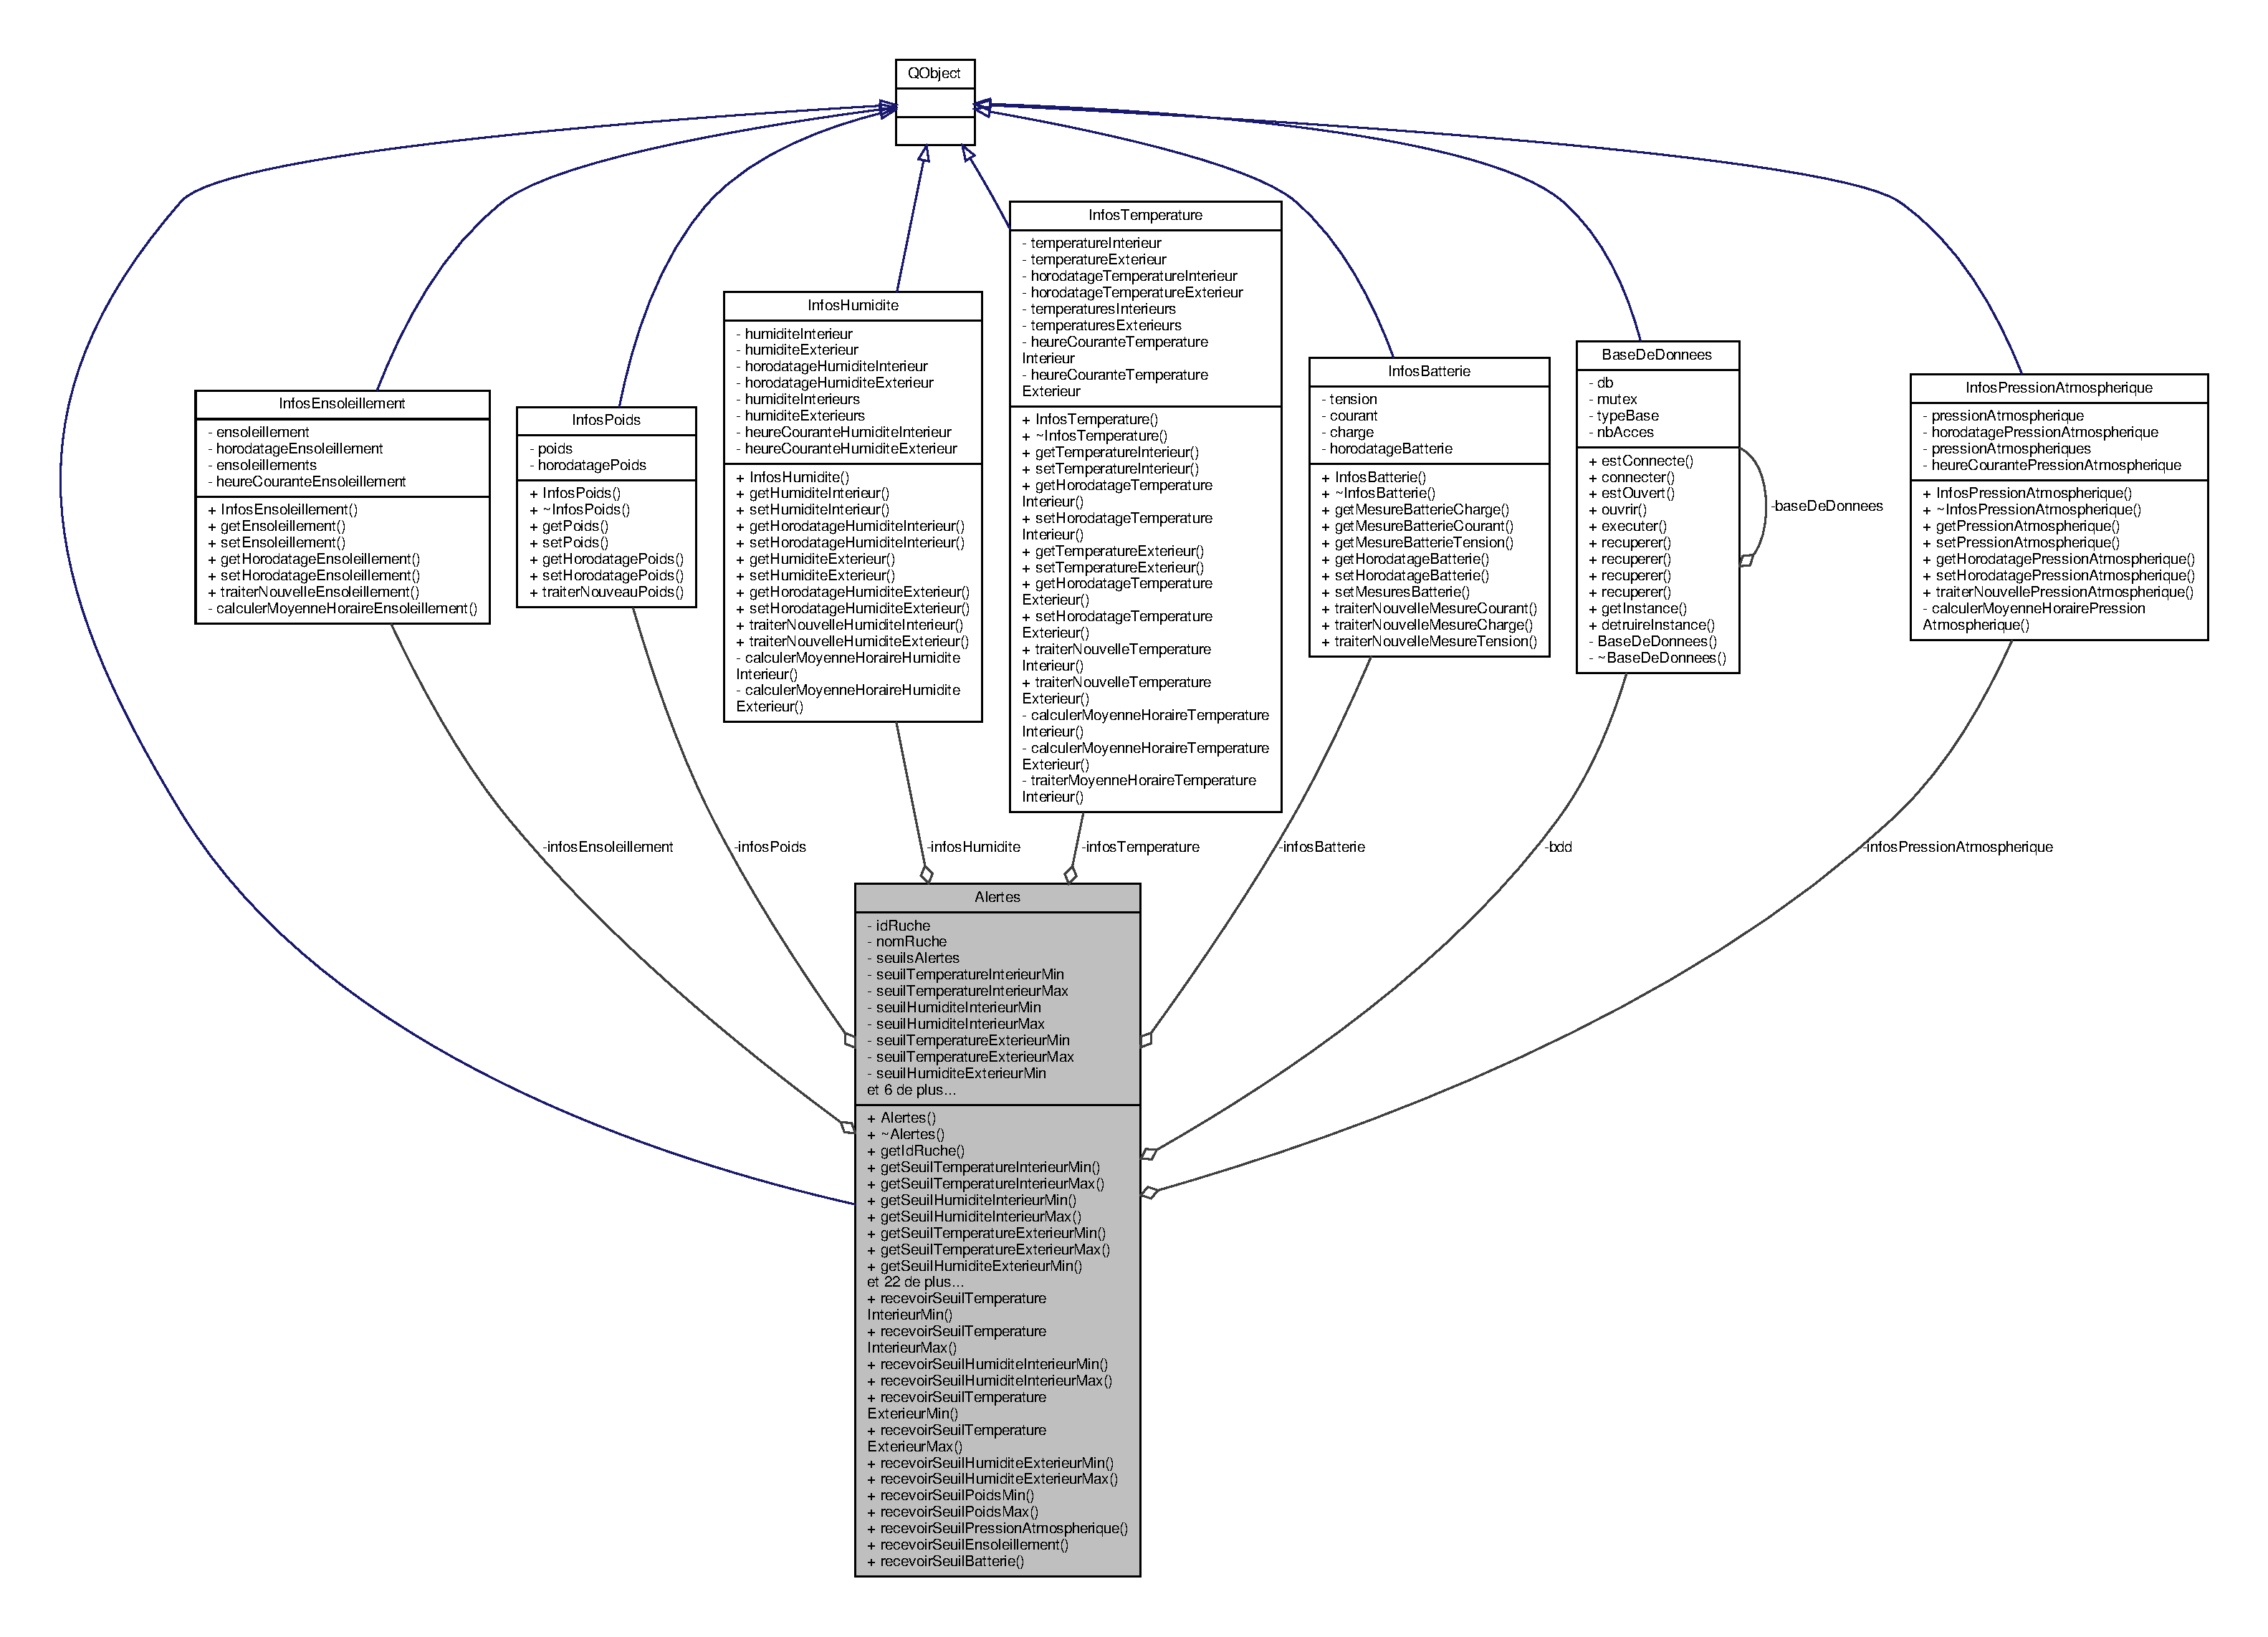
\includegraphics[width=350pt]{class_alertes__coll__graph}
\end{center}
\end{figure}
\subsubsection*{Connecteurs publics}
\begin{DoxyCompactItemize}
\item 
void \hyperlink{class_alertes_a0e5e5177eed435d74bcbdc2a36911e52}{recevoir\+Seuil\+Temperature\+Interieur\+Min} (Q\+String seuil)
\begin{DoxyCompactList}\small\item\em slot de reception des seuils de temperature interieur minimum venant de la classe \hyperlink{class_reglages_alertes_ihm}{Reglages\+Alertes\+Ihm} \end{DoxyCompactList}\item 
void \hyperlink{class_alertes_a06b136f1e86ca97978187305a11be0ff}{recevoir\+Seuil\+Temperature\+Interieur\+Max} (Q\+String seuil)
\begin{DoxyCompactList}\small\item\em slot de reception des seuils de temperature interieur maxmum venant de la classe \hyperlink{class_reglages_alertes_ihm}{Reglages\+Alertes\+Ihm} \end{DoxyCompactList}\item 
void \hyperlink{class_alertes_a4444f527a708f8e1963d2dc1c95bad96}{recevoir\+Seuil\+Humidite\+Interieur\+Min} (Q\+String seuil)
\begin{DoxyCompactList}\small\item\em slot de reception des seuils de humidite interieur minimum venant de la classe \hyperlink{class_reglages_alertes_ihm}{Reglages\+Alertes\+Ihm} \end{DoxyCompactList}\item 
void \hyperlink{class_alertes_a7554e8b6752b0e0a5cfefeecfbc3ba56}{recevoir\+Seuil\+Humidite\+Interieur\+Max} (Q\+String seuil)
\begin{DoxyCompactList}\small\item\em slot de reception des seuils de humidite interieur maximum venant de la classe \hyperlink{class_reglages_alertes_ihm}{Reglages\+Alertes\+Ihm} \end{DoxyCompactList}\item 
void \hyperlink{class_alertes_ad88c760d06e1d438a57027857d50a77f}{recevoir\+Seuil\+Temperature\+Exterieur\+Min} (Q\+String seuil)
\begin{DoxyCompactList}\small\item\em slot de reception des seuils de temperature exterieur minimum venant de la classe \hyperlink{class_reglages_alertes_ihm}{Reglages\+Alertes\+Ihm} \end{DoxyCompactList}\item 
void \hyperlink{class_alertes_af896e03da2f2ec319d410fb8dcc89e0e}{recevoir\+Seuil\+Temperature\+Exterieur\+Max} (Q\+String seuil)
\begin{DoxyCompactList}\small\item\em slot de reception des seuils de temperature exterieur maximum venant de la classe \hyperlink{class_reglages_alertes_ihm}{Reglages\+Alertes\+Ihm} \end{DoxyCompactList}\item 
void \hyperlink{class_alertes_a021d167be6c98d9b0718bb9c7209b47e}{recevoir\+Seuil\+Humidite\+Exterieur\+Min} (Q\+String seuil)
\begin{DoxyCompactList}\small\item\em slot de reception des seuils de humidite exterieur minimum venant de la classe \hyperlink{class_reglages_alertes_ihm}{Reglages\+Alertes\+Ihm} \end{DoxyCompactList}\item 
void \hyperlink{class_alertes_a8c8500d99314034be3c01a871f209fb8}{recevoir\+Seuil\+Humidite\+Exterieur\+Max} (Q\+String seuil)
\begin{DoxyCompactList}\small\item\em slot de reception des seuils de humidite exterieur maximum venant de la classe \hyperlink{class_reglages_alertes_ihm}{Reglages\+Alertes\+Ihm} \end{DoxyCompactList}\item 
void \hyperlink{class_alertes_ab6a15b0c8387a2cdf47dacce92c60383}{recevoir\+Seuil\+Poids\+Min} (Q\+String seuil)
\begin{DoxyCompactList}\small\item\em slot de reception des seuils de poids minimum venant de la classe \hyperlink{class_reglages_alertes_ihm}{Reglages\+Alertes\+Ihm} \end{DoxyCompactList}\item 
void \hyperlink{class_alertes_a77b71a5bc047ced8d09f59a521f58616}{recevoir\+Seuil\+Poids\+Max} (Q\+String seuil)
\begin{DoxyCompactList}\small\item\em slot de reception des seuils de poids maximum venant de la classe \hyperlink{class_reglages_alertes_ihm}{Reglages\+Alertes\+Ihm} \end{DoxyCompactList}\item 
void \hyperlink{class_alertes_a4496c251e1cde3e8c6beee64bad53fe3}{recevoir\+Seuil\+Pression\+Atmospherique} (Q\+String seuil)
\begin{DoxyCompactList}\small\item\em slot de reception des seuils de pression atmospherique venant de la classe \hyperlink{class_reglages_alertes_ihm}{Reglages\+Alertes\+Ihm} \end{DoxyCompactList}\item 
void \hyperlink{class_alertes_abf6b9934820f50024c50dc9691f4ddee}{recevoir\+Seuil\+Ensoleillement} (Q\+String seuil)
\begin{DoxyCompactList}\small\item\em slot de reception des seuils d\textquotesingle{}ensoleillement venant de la classe \hyperlink{class_reglages_alertes_ihm}{Reglages\+Alertes\+Ihm} \end{DoxyCompactList}\item 
void \hyperlink{class_alertes_a61e1f4a105bd64ac829959726ae6ebb8}{recevoir\+Seuil\+Batterie} (Q\+String seuil)
\end{DoxyCompactItemize}
\subsubsection*{Signaux}
\begin{DoxyCompactItemize}
\item 
void \hyperlink{class_alertes_a7726d5049a1453b6c22fafb33693bfe9}{envoi\+Alertes\+Temperature\+Interieur} (\hyperlink{parametres_8h_aaa6de8207c94675264c90b10b613368d}{Seuils\+Alertes})
\item 
void \hyperlink{class_alertes_a7b257375a0d8ad5f41abaa572799aae4}{envoi\+Alertes\+Temperature\+Exterieur} (\hyperlink{parametres_8h_aaa6de8207c94675264c90b10b613368d}{Seuils\+Alertes})
\item 
void \hyperlink{class_alertes_a6d96d5a6e5a1e3c518c45e295a5b4ddf}{envoi\+Alertes\+Humidite\+Interieur} (\hyperlink{parametres_8h_aaa6de8207c94675264c90b10b613368d}{Seuils\+Alertes})
\item 
void \hyperlink{class_alertes_a9a4f2ada9fbf4cf505d6d94831d8e413}{envoi\+Alertes\+Humidite\+Exterieur} (\hyperlink{parametres_8h_aaa6de8207c94675264c90b10b613368d}{Seuils\+Alertes})
\item 
void \hyperlink{class_alertes_a3e81bcca9d4c91c69f575546681590bc}{envoi\+Alertes\+Pression\+Atmospherique} (\hyperlink{parametres_8h_aaa6de8207c94675264c90b10b613368d}{Seuils\+Alertes})
\item 
void \hyperlink{class_alertes_a60f823014dcce3504ee1d78ac50b5328}{envoi\+Alertes\+Poids} (\hyperlink{parametres_8h_aaa6de8207c94675264c90b10b613368d}{Seuils\+Alertes})
\item 
void \hyperlink{class_alertes_a578aa70bc7ca4ec753aa7f97e90f7f02}{envoi\+Alertes\+Ensoleillement} (\hyperlink{parametres_8h_aaa6de8207c94675264c90b10b613368d}{Seuils\+Alertes}, double)
\item 
void \hyperlink{class_alertes_a0e81d795f8e7559eab19fcb9be138f5f}{envoi\+Alertes\+Batterie} (\hyperlink{parametres_8h_aaa6de8207c94675264c90b10b613368d}{Seuils\+Alertes}, double)
\end{DoxyCompactItemize}
\subsubsection*{Fonctions membres publiques}
\begin{DoxyCompactItemize}
\item 
\hyperlink{class_alertes_ad2e4e3907f97bdd06840dfeee0a87ddb}{Alertes} (Q\+String \hyperlink{class_alertes_ae3f9d7aa34ab3c83a66c8484e2b89925}{id\+Ruche}, Q\+String \hyperlink{class_alertes_a212f2a7185bcc7b11f3e54200272bdcf}{nom\+Ruche}, \hyperlink{class_q_object}{Q\+Object} $\ast$parent=0)
\begin{DoxyCompactList}\small\item\em Constructeur de la classe \hyperlink{class_alertes}{Alertes}. \end{DoxyCompactList}\item 
\hyperlink{class_alertes_a730b10861d04de9944b30b11c6b3c3af}{$\sim$\+Alertes} ()
\item 
Q\+String \hyperlink{class_alertes_a2374f9e3e5dc95eacaa4eaa5d98540a7}{get\+Id\+Ruche} ()
\item 
double \hyperlink{class_alertes_af61b11556d97f923cf7dd25ac4f5dd05}{get\+Seuil\+Temperature\+Interieur\+Min} ()
\item 
double \hyperlink{class_alertes_ac514ebef5e7e65aa7bee0ebe3cd7e883}{get\+Seuil\+Temperature\+Interieur\+Max} ()
\item 
double \hyperlink{class_alertes_a40d47b65952035b78cac05b915ad57b8}{get\+Seuil\+Humidite\+Interieur\+Min} ()
\item 
double \hyperlink{class_alertes_a86e0bb83ac1fa5e704e3b7b3fc7147cd}{get\+Seuil\+Humidite\+Interieur\+Max} ()
\item 
double \hyperlink{class_alertes_a4451c6b077256d838e584a073444d83d}{get\+Seuil\+Temperature\+Exterieur\+Min} ()
\item 
double \hyperlink{class_alertes_a00d834877e1fc34d7e0659ef6963ac4f}{get\+Seuil\+Temperature\+Exterieur\+Max} ()
\item 
double \hyperlink{class_alertes_a68e467e042b615f56347a0953d6e64f1}{get\+Seuil\+Humidite\+Exterieur\+Min} ()
\item 
double \hyperlink{class_alertes_ad2c8daf5668f5d122efb9b84f7ea86de}{get\+Seuil\+Humidite\+Exterieur\+Max} ()
\item 
double \hyperlink{class_alertes_a228829e2826ee20cc014b2eb54addf14}{get\+Seuil\+Poids\+Min} ()
\item 
double \hyperlink{class_alertes_a2c19b460f7f7cc7a867b5ed634371878}{get\+Seuil\+Poids\+Max} ()
\item 
double \hyperlink{class_alertes_a502fa36037246fb6eaad1db859bc1971}{get\+Seuil\+Pression\+Atmospherique} ()
\item 
double \hyperlink{class_alertes_a54900058557979664d25137399ae2512}{get\+Seuil\+Ensoleillement} ()
\item 
double \hyperlink{class_alertes_adcf9f9fb707944ae17f2355819eb58d1}{get\+Seuil\+Batterie} ()
\item 
void \hyperlink{class_alertes_a091a0fabca5b06302bc19de31aecafff}{set\+Infos\+Temperature} (\hyperlink{class_infos_temperature}{Infos\+Temperature} $\ast$\hyperlink{class_alertes_ad02b203545812ad6408befecc94ee0ec}{infos\+Temperature})
\item 
void \hyperlink{class_alertes_a05734ac9e97a9001de4ce9ef96235c87}{set\+Infos\+Humidite} (\hyperlink{class_infos_humidite}{Infos\+Humidite} $\ast$\hyperlink{class_alertes_a7b6d798ca0629b474120cd55eb8b510c}{infos\+Humidite})
\item 
void \hyperlink{class_alertes_a771133f26d4ab8c90d1bdf50e1d23d87}{set\+Infos\+Pression\+Atmospherique} (\hyperlink{class_infos_pression_atmospherique}{Infos\+Pression\+Atmospherique} $\ast$\hyperlink{class_alertes_af4bfb245d72bc2eb080df844aa50ac86}{infos\+Pression\+Atmospherique})
\item 
void \hyperlink{class_alertes_a100bad47769994abc976419a355c4a26}{set\+Infos\+Poids} (\hyperlink{class_infos_poids}{Infos\+Poids} $\ast$\hyperlink{class_alertes_add699ea1cebadb371f86b4c47ebe381d}{infos\+Poids})
\item 
void \hyperlink{class_alertes_a8bbe30ddc4893f943781749917b23463}{set\+Infos\+Batterie} (\hyperlink{class_infos_batterie}{Infos\+Batterie} $\ast$\hyperlink{class_alertes_ad5c756a52ff4d6ae85cc0f03bd80582b}{infos\+Batterie})
\item 
void \hyperlink{class_alertes_a5379fc65522a77dc2cc110e489e1469d}{set\+Infos\+Ensoleillement} (\hyperlink{class_infos_ensoleillement}{Infos\+Ensoleillement} $\ast$\hyperlink{class_alertes_abd9b6ff4e9f1df3c360374cceb8d0601}{infos\+Ensoleillement})
\item 
void \hyperlink{class_alertes_a8bc56cf9eb525624b2c1f5b20f86724b}{alertes\+Temperature\+Interieur} ()
\begin{DoxyCompactList}\small\item\em defini les seuils d\textquotesingle{}alertes de la temperature interieur \end{DoxyCompactList}\item 
void \hyperlink{class_alertes_a91fb2665fa8b6c32c74bfe4d1b89a2d8}{alertes\+Temperature\+Exterieur} ()
\begin{DoxyCompactList}\small\item\em defini les seuils d\textquotesingle{}alertes de la temperature exterieur \end{DoxyCompactList}\item 
void \hyperlink{class_alertes_a7558cb097dc392547ceb12ab4d6cbd4c}{alertes\+Humidite\+Interieur} ()
\begin{DoxyCompactList}\small\item\em defini les seuils d\textquotesingle{}alertes de l\textquotesingle{}humidite interieur \end{DoxyCompactList}\item 
void \hyperlink{class_alertes_a8606946eaa04dfd29bb7951b2b850a04}{alertes\+Humidite\+Exterieur} ()
\begin{DoxyCompactList}\small\item\em defini les seuils d\textquotesingle{}alertes de l\textquotesingle{}humidite exterieur \end{DoxyCompactList}\item 
void \hyperlink{class_alertes_ab8a33e82cdd4d4e0560c9ba6e10ca8d5}{alertes\+Pression\+Atmospherique} ()
\begin{DoxyCompactList}\small\item\em defini les seuils d\textquotesingle{}alertes de pression atmospherique \end{DoxyCompactList}\item 
void \hyperlink{class_alertes_ac4b8925cc6c262cf7254b1576ba07d33}{alertes\+Poids} ()
\begin{DoxyCompactList}\small\item\em defini les seuils d\textquotesingle{}alertes de poids \end{DoxyCompactList}\item 
void \hyperlink{class_alertes_ae7ad960c530a6a7e82df3ed55d159a68}{alertes\+Ensoleillement} ()
\begin{DoxyCompactList}\small\item\em defini les seuils d\textquotesingle{}alertes d\textquotesingle{}ensoleillement \end{DoxyCompactList}\item 
void \hyperlink{class_alertes_ad708a4b800d56c1439b65d12a3c6b027}{alertes\+Batterie} ()
\item 
void \hyperlink{class_alertes_ad04a02dcc6e6f14da0784c7054888b05}{appeler\+Les\+Alertes} (\hyperlink{parametres_8h_a83a725fd153179a2bd97afcc8307737b}{Type\+Alertes} type\+Alertes)
\begin{DoxyCompactList}\small\item\em defini les différents appels des alertes \end{DoxyCompactList}\item 
void \hyperlink{class_alertes_a375783502a78109f3323dc1ed90cfdc9}{envoyer\+Mail\+Alerte} (Q\+String email, Q\+String objet, Q\+String message)
\end{DoxyCompactItemize}
\subsubsection*{Attributs privés}
\begin{DoxyCompactItemize}
\item 
Q\+String \hyperlink{class_alertes_ae3f9d7aa34ab3c83a66c8484e2b89925}{id\+Ruche}
\item 
Q\+String \hyperlink{class_alertes_a212f2a7185bcc7b11f3e54200272bdcf}{nom\+Ruche}
\item 
\hyperlink{class_infos_temperature}{Infos\+Temperature} $\ast$ \hyperlink{class_alertes_ad02b203545812ad6408befecc94ee0ec}{infos\+Temperature}
\item 
\hyperlink{class_infos_humidite}{Infos\+Humidite} $\ast$ \hyperlink{class_alertes_a7b6d798ca0629b474120cd55eb8b510c}{infos\+Humidite}
\item 
\hyperlink{class_infos_pression_atmospherique}{Infos\+Pression\+Atmospherique} $\ast$ \hyperlink{class_alertes_af4bfb245d72bc2eb080df844aa50ac86}{infos\+Pression\+Atmospherique}
\item 
\hyperlink{class_infos_ensoleillement}{Infos\+Ensoleillement} $\ast$ \hyperlink{class_alertes_abd9b6ff4e9f1df3c360374cceb8d0601}{infos\+Ensoleillement}
\item 
\hyperlink{class_infos_batterie}{Infos\+Batterie} $\ast$ \hyperlink{class_alertes_ad5c756a52ff4d6ae85cc0f03bd80582b}{infos\+Batterie}
\item 
\hyperlink{class_infos_poids}{Infos\+Poids} $\ast$ \hyperlink{class_alertes_add699ea1cebadb371f86b4c47ebe381d}{infos\+Poids}
\item 
\hyperlink{parametres_8h_aaa6de8207c94675264c90b10b613368d}{Seuils\+Alertes} \hyperlink{class_alertes_adedb6924af18a7f7a14b11ffa33db6ba}{seuils\+Alertes}
\item 
\hyperlink{class_base_de_donnees}{Base\+De\+Donnees} $\ast$ \hyperlink{class_alertes_a91e58b69d29922e8e984efb767ae5268}{bdd}
\begin{DoxyCompactList}\small\item\em agrégation de l\textquotesingle{}objet \hyperlink{class_base_de_donnees}{Base\+De\+Donnees} \end{DoxyCompactList}\item 
double \hyperlink{class_alertes_a1c970252300a177bef641ca5399d3783}{seuil\+Temperature\+Interieur\+Min}
\item 
double \hyperlink{class_alertes_abeda87298576a3b3eefcca9a96b8a0a9}{seuil\+Temperature\+Interieur\+Max}
\item 
double \hyperlink{class_alertes_a501773587c8f2ccd032fe7db9af1f4e2}{seuil\+Humidite\+Interieur\+Min}
\item 
double \hyperlink{class_alertes_a795cd3721854335f6c91e6009b324c37}{seuil\+Humidite\+Interieur\+Max}
\item 
double \hyperlink{class_alertes_a0898c501edf5f07ac503b31b8a3d2454}{seuil\+Temperature\+Exterieur\+Min}
\item 
double \hyperlink{class_alertes_a207e0266c68ad378dae846382ba9f9dc}{seuil\+Temperature\+Exterieur\+Max}
\item 
double \hyperlink{class_alertes_a18afbc02513a6e4fa8baa665092719c9}{seuil\+Humidite\+Exterieur\+Min}
\item 
double \hyperlink{class_alertes_afa54793d1f47a97894faf91e76fb2a04}{seuil\+Humidite\+Exterieur\+Max}
\item 
double \hyperlink{class_alertes_a3f23bee8122888916e33559f4d0bf34b}{seuil\+Poids\+Min}
\item 
double \hyperlink{class_alertes_a19b88c68325ccc6e5e8ad11a2537b25e}{seuil\+Poids\+Max}
\item 
double \hyperlink{class_alertes_a7f512b6d3b5bc0851757ab4d18279ccf}{seuil\+Ensoleillement}
\item 
double \hyperlink{class_alertes_a565094789ef5eb0ae2a2a562ee8a9704}{seuil\+Pression\+Atmospherique}
\item 
double \hyperlink{class_alertes_a3ac4e5d2b1a8fdd9cf4633861948110f}{seuil\+Batterie}
\end{DoxyCompactItemize}


\subsubsection{Description détaillée}
\begin{DoxyAuthor}{Auteur}
Florentin Mellah, Enzo Rossi
\end{DoxyAuthor}
\begin{DoxyVersion}{Version}
1.\+1 
\end{DoxyVersion}


\subsubsection{Documentation des constructeurs et destructeur}
\mbox{\Hypertarget{class_alertes_ad2e4e3907f97bdd06840dfeee0a87ddb}\label{class_alertes_ad2e4e3907f97bdd06840dfeee0a87ddb}} 
\index{Alertes@{Alertes}!Alertes@{Alertes}}
\index{Alertes@{Alertes}!Alertes@{Alertes}}
\paragraph{\texorpdfstring{Alertes()}{Alertes()}}
{\footnotesize\ttfamily Alertes\+::\+Alertes (\begin{DoxyParamCaption}\item[{Q\+String}]{id\+Ruche,  }\item[{Q\+String}]{nom\+Ruche,  }\item[{\hyperlink{class_q_object}{Q\+Object} $\ast$}]{parent = {\ttfamily 0} }\end{DoxyParamCaption})\hspace{0.3cm}{\ttfamily [explicit]}}

Définition des attributs de la classe \hyperlink{class_alertes}{Alertes} 

Références \hyperlink{class_alertes_a91e58b69d29922e8e984efb767ae5268}{bdd}, \hyperlink{parametres_8h_a45f8f15b8f9a7ab4c2b219038ff64f6b}{B\+D\+D\+\_\+\+N\+O\+M\+B\+A\+SE}, \hyperlink{parametres_8h_ae2ded9166ed2553182545e97514c04f7}{B\+D\+D\+\_\+\+P\+A\+S\+S\+W\+O\+RD}, \hyperlink{parametres_8h_a423559dc987673b8aacaa9f369839bb0}{B\+D\+D\+\_\+\+S\+E\+R\+V\+E\+UR}, \hyperlink{parametres_8h_a88b5f5b81fa534553c68802384beff2c}{B\+D\+D\+\_\+\+U\+S\+E\+R\+N\+A\+ME}, \hyperlink{class_base_de_donnees_ac20da193923a9bfea5e38ee5a54820cd}{Base\+De\+Donnees\+::connecter()}, \hyperlink{class_base_de_donnees_a00388973f3ec42e5c8e76e7af7e124b2}{Base\+De\+Donnees\+::est\+Connecte()}, \hyperlink{class_base_de_donnees_a80028aa2b6b4fbf30fb2e36357b7d3d3}{Base\+De\+Donnees\+::get\+Instance()}, et \hyperlink{class_base_de_donnees_a77539baad389f5acf754cd2cd452403e}{Base\+De\+Donnees\+::recuperer()}.


\begin{DoxyCode}
00038                                                                    : \hyperlink{class_q_object}{QObject}(parent), 
      \hyperlink{class_alertes_ae3f9d7aa34ab3c83a66c8484e2b89925}{idRuche}(\hyperlink{class_alertes_ae3f9d7aa34ab3c83a66c8484e2b89925}{idRuche}), \hyperlink{class_alertes_a212f2a7185bcc7b11f3e54200272bdcf}{nomRuche}(\hyperlink{class_alertes_a212f2a7185bcc7b11f3e54200272bdcf}{nomRuche}), 
      \hyperlink{class_alertes_ad02b203545812ad6408befecc94ee0ec}{infosTemperature}(0), \hyperlink{class_alertes_a7b6d798ca0629b474120cd55eb8b510c}{infosHumidite}(0), 
      \hyperlink{class_alertes_af4bfb245d72bc2eb080df844aa50ac86}{infosPressionAtmospherique}(0),
00039     \hyperlink{class_alertes_a1c970252300a177bef641ca5399d3783}{seuilTemperatureInterieurMin}(
      \hyperlink{parametres_8h_a1f78dd3105c514060033c23f7b40a899}{TEMPERATURE\_INTERIEUR\_SEUIL\_MIN}), 
      \hyperlink{class_alertes_abeda87298576a3b3eefcca9a96b8a0a9}{seuilTemperatureInterieurMax}(
      \hyperlink{parametres_8h_a76f490066655530a774202e6204f2a92}{TEMPERATURE\_INTERIEUR\_SEUIL\_MAX}), 
      \hyperlink{class_alertes_a501773587c8f2ccd032fe7db9af1f4e2}{seuilHumiditeInterieurMin}(\hyperlink{parametres_8h_a123e6e1d82333f6e038d37ef506d5762}{HUMIDITE\_INTERIEUR\_SEUIL\_MIN}
      ), \hyperlink{class_alertes_a795cd3721854335f6c91e6009b324c37}{seuilHumiditeInterieurMax}(
      \hyperlink{parametres_8h_afc1996946dfec64accdaa88f4e313058}{HUMIDITE\_INTERIEUR\_SEUIL\_MAX}), 
      \hyperlink{class_alertes_a0898c501edf5f07ac503b31b8a3d2454}{seuilTemperatureExterieurMin}(
      \hyperlink{parametres_8h_aeb90c8fd31e6aa6473edd143ce70e137}{TEMPERATURE\_EXTERIEUR\_SEUIL\_MIN}), 
      \hyperlink{class_alertes_a207e0266c68ad378dae846382ba9f9dc}{seuilTemperatureExterieurMax}(
      \hyperlink{parametres_8h_a7630cd07e0f037b4057157febd9644fd}{TEMPERATURE\_EXTERIEUR\_SEUIL\_MAX}), 
      \hyperlink{class_alertes_a18afbc02513a6e4fa8baa665092719c9}{seuilHumiditeExterieurMin}(\hyperlink{parametres_8h_afc00f65688c19bd56711c244827c2c27}{HUMIDITE\_EXTERIEUR\_SEUIL\_MIN}
      ), \hyperlink{class_alertes_afa54793d1f47a97894faf91e76fb2a04}{seuilHumiditeExterieurMax}(
      \hyperlink{parametres_8h_a25f8411ff3fd72788fdcd7487e7e8d28}{HUMIDITE\_EXTERIEUR\_SEUIL\_MAX}), \hyperlink{class_alertes_a3f23bee8122888916e33559f4d0bf34b}{seuilPoidsMin}(
      \hyperlink{parametres_8h_a289e59d08fbd111c6a5bd8a526a8098b}{POIDS\_SEUIL\_MIN}), \hyperlink{class_alertes_a19b88c68325ccc6e5e8ad11a2537b25e}{seuilPoidsMax}(\hyperlink{parametres_8h_a41d2727214068bc11cea2e021fb6b237}{POIDS\_SEUIL\_MAX}), 
      \hyperlink{class_alertes_a7f512b6d3b5bc0851757ab4d18279ccf}{seuilEnsoleillement}(\hyperlink{parametres_8h_a1174d9c2d3ff7e8a5e464d7e0a20e1a9}{ENSOLEILLEMENT\_SEUIL\_MIN}), 
      \hyperlink{class_alertes_a565094789ef5eb0ae2a2a562ee8a9704}{seuilPressionAtmospherique}(
      \hyperlink{parametres_8h_a70a55fd4037201bf606fc9e9d54e61cb}{PRESSION\_ATMOSPHERIQUE\_SEUIL\_MIN})
00040 
00041 \{
00042     \hyperlink{class_alertes_a91e58b69d29922e8e984efb767ae5268}{bdd} = \hyperlink{class_base_de_donnees_a80028aa2b6b4fbf30fb2e36357b7d3d3}{BaseDeDonnees::getInstance}();
00043     \textcolor{keywordflow}{if}(!\hyperlink{class_alertes_a91e58b69d29922e8e984efb767ae5268}{bdd}->\hyperlink{class_base_de_donnees_a00388973f3ec42e5c8e76e7af7e124b2}{estConnecte}())
00044         \hyperlink{class_alertes_a91e58b69d29922e8e984efb767ae5268}{bdd}->\hyperlink{class_base_de_donnees_ac20da193923a9bfea5e38ee5a54820cd}{connecter}(\hyperlink{parametres_8h_a45f8f15b8f9a7ab4c2b219038ff64f6b}{BDD\_NOMBASE}, \hyperlink{parametres_8h_a88b5f5b81fa534553c68802384beff2c}{BDD\_USERNAME}, 
      \hyperlink{parametres_8h_ae2ded9166ed2553182545e97514c04f7}{BDD\_PASSWORD}, \hyperlink{parametres_8h_a423559dc987673b8aacaa9f369839bb0}{BDD\_SERVEUR});
00045 
00046     QStringList seuils;
00047     QString requete = \textcolor{stringliteral}{"SELECT * FROM Seuils WHERE idRuche='"} + \hyperlink{class_alertes_ae3f9d7aa34ab3c83a66c8484e2b89925}{idRuche} + \textcolor{stringliteral}{"'"};
00048     qDebug()<< Q\_FUNC\_INFO << requete;
00049     \textcolor{keywordtype}{bool} retour = \hyperlink{class_alertes_a91e58b69d29922e8e984efb767ae5268}{bdd}->\hyperlink{class_base_de_donnees_a77539baad389f5acf754cd2cd452403e}{recuperer}(requete, seuils);
00050     \textcolor{keywordflow}{if}(retour)
00051     \{
00052         qDebug() << Q\_FUNC\_INFO << seuils;
00053         \textcolor{comment}{/*seuilTemperatureInterieurMin = seuils.at(1).toDouble();}
00054 \textcolor{comment}{        seuilTemperatureInterieurMax = ;}
00055 \textcolor{comment}{        seuilHumiditeInterieurMin = ;}
00056 \textcolor{comment}{        seuilHumiditeInterieurMax = ;}
00057 \textcolor{comment}{        seuilTemperatureExterieurMin = ;}
00058 \textcolor{comment}{        seuilTemperatureExterieurMax = ;}
00059 \textcolor{comment}{        seuilHumiditeExterieurMin = ;}
00060 \textcolor{comment}{        seuilHumiditeExterieurMax = ;}
00061 \textcolor{comment}{        seuilPoidsMin = ;}
00062 \textcolor{comment}{        seuilPoidsMax = ;}
00063 \textcolor{comment}{        seuilEnsoleillement = ;}
00064 \textcolor{comment}{        seuilPressionAtmospherique = ;*/}
00065     \}
00066 \}
\end{DoxyCode}
\mbox{\Hypertarget{class_alertes_a730b10861d04de9944b30b11c6b3c3af}\label{class_alertes_a730b10861d04de9944b30b11c6b3c3af}} 
\index{Alertes@{Alertes}!````~Alertes@{$\sim$\+Alertes}}
\index{````~Alertes@{$\sim$\+Alertes}!Alertes@{Alertes}}
\paragraph{\texorpdfstring{$\sim$\+Alertes()}{~Alertes()}}
{\footnotesize\ttfamily Alertes\+::$\sim$\+Alertes (\begin{DoxyParamCaption}{ }\end{DoxyParamCaption})}



Références \hyperlink{class_base_de_donnees_a457401c0816b888c77ce915997545f4e}{Base\+De\+Donnees\+::detruire\+Instance()}.


\begin{DoxyCode}
00069 \{
00070     \hyperlink{class_base_de_donnees_a457401c0816b888c77ce915997545f4e}{BaseDeDonnees::detruireInstance}();
00071 \}
\end{DoxyCode}


\subsubsection{Documentation des fonctions membres}
\mbox{\Hypertarget{class_alertes_ad708a4b800d56c1439b65d12a3c6b027}\label{class_alertes_ad708a4b800d56c1439b65d12a3c6b027}} 
\index{Alertes@{Alertes}!alertes\+Batterie@{alertes\+Batterie}}
\index{alertes\+Batterie@{alertes\+Batterie}!Alertes@{Alertes}}
\paragraph{\texorpdfstring{alertes\+Batterie()}{alertesBatterie()}}
{\footnotesize\ttfamily void Alertes\+::alertes\+Batterie (\begin{DoxyParamCaption}{ }\end{DoxyParamCaption})}



Références \hyperlink{class_alertes_a91e58b69d29922e8e984efb767ae5268}{bdd}, \hyperlink{parametres_8h_aaa6de8207c94675264c90b10b613368da5ac8ec3b54d90a07c6bb5a77ef971821}{bon}, \hyperlink{class_alertes_a0e81d795f8e7559eab19fcb9be138f5f}{envoi\+Alertes\+Batterie()}, \hyperlink{class_alertes_a375783502a78109f3323dc1ed90cfdc9}{envoyer\+Mail\+Alerte()}, \hyperlink{class_infos_batterie_a8c37174d0d36e4f5ada9d16dd5894803}{Infos\+Batterie\+::get\+Mesure\+Batterie\+Charge()}, \hyperlink{class_alertes_ad5c756a52ff4d6ae85cc0f03bd80582b}{infos\+Batterie}, \hyperlink{class_alertes_a212f2a7185bcc7b11f3e54200272bdcf}{nom\+Ruche}, \hyperlink{class_base_de_donnees_a77539baad389f5acf754cd2cd452403e}{Base\+De\+Donnees\+::recuperer()}, \hyperlink{class_alertes_a3ac4e5d2b1a8fdd9cf4633861948110f}{seuil\+Batterie}, et \hyperlink{parametres_8h_aaa6de8207c94675264c90b10b613368da4257e2f8921856770c8266f55c937295}{trop\+Bas}.



Référencé par \hyperlink{class_alertes_ad04a02dcc6e6f14da0784c7054888b05}{appeler\+Les\+Alertes()}.


\begin{DoxyCode}
00408 \{
00409     \textcolor{keywordtype}{double} mesureBatterie = \hyperlink{class_alertes_ad5c756a52ff4d6ae85cc0f03bd80582b}{infosBatterie}->\hyperlink{class_infos_batterie_a8c37174d0d36e4f5ada9d16dd5894803}{getMesureBatterieCharge}();
00410     QString requete = \textcolor{stringliteral}{"SELECT Email FROM Apiculteur WHERE idApiculteur = '3'"};
00411     QString mailApiculteur;
00412     \hyperlink{class_alertes_a91e58b69d29922e8e984efb767ae5268}{bdd}->\hyperlink{class_base_de_donnees_a77539baad389f5acf754cd2cd452403e}{recuperer}(requete, mailApiculteur);
00413 
00414     qDebug() << Q\_FUNC\_INFO << \textcolor{stringliteral}{"mesureBatterie"} << mesureBatterie << \textcolor{stringliteral}{"seuilBatterie"} << 
      \hyperlink{class_alertes_a3ac4e5d2b1a8fdd9cf4633861948110f}{seuilBatterie};
00415 
00416     \textcolor{keywordflow}{if}(mesureBatterie < seuilBatterie)
00417     \{
00418         emit \hyperlink{class_alertes_a0e81d795f8e7559eab19fcb9be138f5f}{envoiAlertesBatterie}(\hyperlink{parametres_8h_aaa6de8207c94675264c90b10b613368da4257e2f8921856770c8266f55c937295}{tropBas}, mesureBatterie);
00419         \hyperlink{class_alertes_a375783502a78109f3323dc1ed90cfdc9}{envoyerMailAlerte}(mailApiculteur, \textcolor{stringliteral}{"Alerte Batterie"}, \textcolor{stringliteral}{"Bonjour, une alerte a été
       détectée dans la "}  + \hyperlink{class_alertes_a212f2a7185bcc7b11f3e54200272bdcf}{nomRuche} +  \textcolor{stringliteral}{" : niveau de batterie faible."});
00420     \}
00421     \textcolor{keywordflow}{else}
00422     \{
00423         emit \hyperlink{class_alertes_a0e81d795f8e7559eab19fcb9be138f5f}{envoiAlertesBatterie}(\hyperlink{parametres_8h_aaa6de8207c94675264c90b10b613368da5ac8ec3b54d90a07c6bb5a77ef971821}{bon}, mesureBatterie);
00424     \}
00425 \}
\end{DoxyCode}
\mbox{\Hypertarget{class_alertes_ae7ad960c530a6a7e82df3ed55d159a68}\label{class_alertes_ae7ad960c530a6a7e82df3ed55d159a68}} 
\index{Alertes@{Alertes}!alertes\+Ensoleillement@{alertes\+Ensoleillement}}
\index{alertes\+Ensoleillement@{alertes\+Ensoleillement}!Alertes@{Alertes}}
\paragraph{\texorpdfstring{alertes\+Ensoleillement()}{alertesEnsoleillement()}}
{\footnotesize\ttfamily void Alertes\+::alertes\+Ensoleillement (\begin{DoxyParamCaption}{ }\end{DoxyParamCaption})}

\begin{DoxyReturn}{Renvoie}
{\itshape trop\+Haut} est definit dans le type enum Seuils\+Alertes et retourne 0 

{\itshape trop\+Bas} est definit dans le type enum Seuils\+Alertes et retourne 1 

{\itshape bon} est definit dans le type enum Seuils\+Alertes et retourne 2 
\end{DoxyReturn}


Références \hyperlink{class_alertes_a91e58b69d29922e8e984efb767ae5268}{bdd}, \hyperlink{parametres_8h_aaa6de8207c94675264c90b10b613368da5ac8ec3b54d90a07c6bb5a77ef971821}{bon}, \hyperlink{class_alertes_a578aa70bc7ca4ec753aa7f97e90f7f02}{envoi\+Alertes\+Ensoleillement()}, \hyperlink{class_infos_ensoleillement_a388dd7b2ae97839a779ca1384ca8e6e2}{Infos\+Ensoleillement\+::get\+Ensoleillement()}, \hyperlink{class_alertes_abd9b6ff4e9f1df3c360374cceb8d0601}{infos\+Ensoleillement}, \hyperlink{class_base_de_donnees_a77539baad389f5acf754cd2cd452403e}{Base\+De\+Donnees\+::recuperer()}, \hyperlink{class_alertes_a7f512b6d3b5bc0851757ab4d18279ccf}{seuil\+Ensoleillement}, et \hyperlink{parametres_8h_aaa6de8207c94675264c90b10b613368da4257e2f8921856770c8266f55c937295}{trop\+Bas}.



Référencé par \hyperlink{class_alertes_ad04a02dcc6e6f14da0784c7054888b05}{appeler\+Les\+Alertes()}.


\begin{DoxyCode}
00387 \{
00388     \textcolor{keywordtype}{double} mesureEnsoleillement = \hyperlink{class_alertes_abd9b6ff4e9f1df3c360374cceb8d0601}{infosEnsoleillement}->
      \hyperlink{class_infos_ensoleillement_a388dd7b2ae97839a779ca1384ca8e6e2}{getEnsoleillement}();
00389     QString requete = \textcolor{stringliteral}{"SELECT Email FROM Apiculteur WHERE idApiculteur = '3'"};
00390     QString mailApiculteur;
00391     \hyperlink{class_alertes_a91e58b69d29922e8e984efb767ae5268}{bdd}->\hyperlink{class_base_de_donnees_a77539baad389f5acf754cd2cd452403e}{recuperer}(requete, mailApiculteur);
00392 
00393     qDebug() << Q\_FUNC\_INFO << \textcolor{stringliteral}{"mesureEnsoleillement"} << mesureEnsoleillement << \textcolor{stringliteral}{"seuilEnsoleillement"} << 
      \hyperlink{class_alertes_a7f512b6d3b5bc0851757ab4d18279ccf}{seuilEnsoleillement};
00394 
00395     \textcolor{keywordflow}{if} (mesureEnsoleillement < seuilEnsoleillement)
00396     \{
00397         qDebug() << Q\_FUNC\_INFO << \textcolor{stringliteral}{"TROP BAS"};
00398         emit \hyperlink{class_alertes_a578aa70bc7ca4ec753aa7f97e90f7f02}{envoiAlertesEnsoleillement}(\hyperlink{parametres_8h_aaa6de8207c94675264c90b10b613368da4257e2f8921856770c8266f55c937295}{tropBas}, mesureEnsoleillement);
00399     \}
00400     \textcolor{keywordflow}{else}
00401     \{
00402         qDebug() << Q\_FUNC\_INFO << \textcolor{stringliteral}{"CORRECT"};
00403         emit \hyperlink{class_alertes_a578aa70bc7ca4ec753aa7f97e90f7f02}{envoiAlertesEnsoleillement}(\hyperlink{parametres_8h_aaa6de8207c94675264c90b10b613368da5ac8ec3b54d90a07c6bb5a77ef971821}{bon}, mesureEnsoleillement);
00404     \}
00405 \}
\end{DoxyCode}
\mbox{\Hypertarget{class_alertes_a8606946eaa04dfd29bb7951b2b850a04}\label{class_alertes_a8606946eaa04dfd29bb7951b2b850a04}} 
\index{Alertes@{Alertes}!alertes\+Humidite\+Exterieur@{alertes\+Humidite\+Exterieur}}
\index{alertes\+Humidite\+Exterieur@{alertes\+Humidite\+Exterieur}!Alertes@{Alertes}}
\paragraph{\texorpdfstring{alertes\+Humidite\+Exterieur()}{alertesHumiditeExterieur()}}
{\footnotesize\ttfamily void Alertes\+::alertes\+Humidite\+Exterieur (\begin{DoxyParamCaption}{ }\end{DoxyParamCaption})}

\begin{DoxyReturn}{Renvoie}
{\itshape trop\+Haut} est definit dans le type enum Seuils\+Alertes et retourne 0 

{\itshape trop\+Bas} est definit dans le type enum Seuils\+Alertes et retourne 1 

{\itshape bon} est definit dans le type enum Seuils\+Alertes et retourne 2 
\end{DoxyReturn}


Références \hyperlink{class_alertes_a91e58b69d29922e8e984efb767ae5268}{bdd}, \hyperlink{parametres_8h_aaa6de8207c94675264c90b10b613368da5ac8ec3b54d90a07c6bb5a77ef971821}{bon}, \hyperlink{class_alertes_a9a4f2ada9fbf4cf505d6d94831d8e413}{envoi\+Alertes\+Humidite\+Exterieur()}, \hyperlink{class_alertes_a375783502a78109f3323dc1ed90cfdc9}{envoyer\+Mail\+Alerte()}, \hyperlink{class_infos_humidite_a23e537fdfa33336a3970838f445387ce}{Infos\+Humidite\+::get\+Humidite\+Exterieur()}, \hyperlink{class_alertes_a7b6d798ca0629b474120cd55eb8b510c}{infos\+Humidite}, \hyperlink{class_alertes_a212f2a7185bcc7b11f3e54200272bdcf}{nom\+Ruche}, \hyperlink{class_base_de_donnees_a77539baad389f5acf754cd2cd452403e}{Base\+De\+Donnees\+::recuperer()}, \hyperlink{class_alertes_afa54793d1f47a97894faf91e76fb2a04}{seuil\+Humidite\+Exterieur\+Max}, \hyperlink{class_alertes_a18afbc02513a6e4fa8baa665092719c9}{seuil\+Humidite\+Exterieur\+Min}, \hyperlink{parametres_8h_aaa6de8207c94675264c90b10b613368da4257e2f8921856770c8266f55c937295}{trop\+Bas}, et \hyperlink{parametres_8h_aaa6de8207c94675264c90b10b613368dabc650d9700ae19f2696e6a6e3f9ab067}{trop\+Haut}.



Référencé par \hyperlink{class_alertes_ad04a02dcc6e6f14da0784c7054888b05}{appeler\+Les\+Alertes()}.


\begin{DoxyCode}
00292 \{
00293     \textcolor{keywordtype}{double} mesureHumiditeExterieur = \hyperlink{class_alertes_a7b6d798ca0629b474120cd55eb8b510c}{infosHumidite}->
      \hyperlink{class_infos_humidite_a23e537fdfa33336a3970838f445387ce}{getHumiditeExterieur}();
00294     QString requete = \textcolor{stringliteral}{"SELECT Email FROM Apiculteur WHERE idApiculteur = '3'"};
00295     QString mailApiculteur;
00296     \hyperlink{class_alertes_a91e58b69d29922e8e984efb767ae5268}{bdd}->\hyperlink{class_base_de_donnees_a77539baad389f5acf754cd2cd452403e}{recuperer}(requete, mailApiculteur);
00297 
00298     qDebug() << Q\_FUNC\_INFO << \textcolor{stringliteral}{"mesureHumiditeExterieur"} << mesureHumiditeExterieur << \textcolor{stringliteral}{"
      seuilHumiditeExterieurMax"} << \hyperlink{class_alertes_afa54793d1f47a97894faf91e76fb2a04}{seuilHumiditeExterieurMax} << \textcolor{stringliteral}{"seuilHumiditeExterieurMin"} << 
      \hyperlink{class_alertes_a18afbc02513a6e4fa8baa665092719c9}{seuilHumiditeExterieurMin};
00299 
00300     \textcolor{keywordflow}{if}(mesureHumiditeExterieur > \hyperlink{class_alertes_afa54793d1f47a97894faf91e76fb2a04}{seuilHumiditeExterieurMax})
00301     \{
00302         emit \hyperlink{class_alertes_a9a4f2ada9fbf4cf505d6d94831d8e413}{envoiAlertesHumiditeExterieur}(\hyperlink{parametres_8h_aaa6de8207c94675264c90b10b613368dabc650d9700ae19f2696e6a6e3f9ab067}{tropHaut});
00303         \hyperlink{class_alertes_a375783502a78109f3323dc1ed90cfdc9}{envoyerMailAlerte}(mailApiculteur, \textcolor{stringliteral}{"Alerte Extérieur Intérieur"}, \textcolor{stringliteral}{"Bonjour, une
       alerte a été détectée dans la "}  + \hyperlink{class_alertes_a212f2a7185bcc7b11f3e54200272bdcf}{nomRuche} +  \textcolor{stringliteral}{": humidité Extérieur élevée."});
00304         qDebug() << Q\_FUNC\_INFO << \textcolor{stringliteral}{"TROP HAUT"};
00305     \}
00306     \textcolor{keywordflow}{else} \textcolor{keywordflow}{if} (mesureHumiditeExterieur < seuilHumiditeExterieurMin)
00307     \{
00308         qDebug() << Q\_FUNC\_INFO << \textcolor{stringliteral}{"TROP BAS"};
00309         emit \hyperlink{class_alertes_a9a4f2ada9fbf4cf505d6d94831d8e413}{envoiAlertesHumiditeExterieur}(\hyperlink{parametres_8h_aaa6de8207c94675264c90b10b613368da4257e2f8921856770c8266f55c937295}{tropBas});
00310         \hyperlink{class_alertes_a375783502a78109f3323dc1ed90cfdc9}{envoyerMailAlerte}(mailApiculteur, \textcolor{stringliteral}{"Alerte Extérieur Intérieur"}, \textcolor{stringliteral}{"Bonjour, une
       alerte a été détectée dans la "}  + \hyperlink{class_alertes_a212f2a7185bcc7b11f3e54200272bdcf}{nomRuche} +  \textcolor{stringliteral}{": humidité Extérieur basse."});
00311     \}
00312     \textcolor{keywordflow}{else}
00313     \{
00314         qDebug() << Q\_FUNC\_INFO << \textcolor{stringliteral}{"CORRECT"};
00315         emit \hyperlink{class_alertes_a9a4f2ada9fbf4cf505d6d94831d8e413}{envoiAlertesHumiditeExterieur}(\hyperlink{parametres_8h_aaa6de8207c94675264c90b10b613368da5ac8ec3b54d90a07c6bb5a77ef971821}{bon});
00316     \}
00317 \}
\end{DoxyCode}
\mbox{\Hypertarget{class_alertes_a7558cb097dc392547ceb12ab4d6cbd4c}\label{class_alertes_a7558cb097dc392547ceb12ab4d6cbd4c}} 
\index{Alertes@{Alertes}!alertes\+Humidite\+Interieur@{alertes\+Humidite\+Interieur}}
\index{alertes\+Humidite\+Interieur@{alertes\+Humidite\+Interieur}!Alertes@{Alertes}}
\paragraph{\texorpdfstring{alertes\+Humidite\+Interieur()}{alertesHumiditeInterieur()}}
{\footnotesize\ttfamily void Alertes\+::alertes\+Humidite\+Interieur (\begin{DoxyParamCaption}{ }\end{DoxyParamCaption})}

\begin{DoxyReturn}{Renvoie}
{\itshape trop\+Haut} est definit dans le type enum Seuils\+Alertes et retourne 0 

{\itshape trop\+Bas} est definit dans le type enum Seuils\+Alertes et retourne 1 

{\itshape bon} est definit dans le type enum Seuils\+Alertes et retourne 2 
\end{DoxyReturn}


Références \hyperlink{class_alertes_a91e58b69d29922e8e984efb767ae5268}{bdd}, \hyperlink{parametres_8h_aaa6de8207c94675264c90b10b613368da5ac8ec3b54d90a07c6bb5a77ef971821}{bon}, \hyperlink{class_alertes_a6d96d5a6e5a1e3c518c45e295a5b4ddf}{envoi\+Alertes\+Humidite\+Interieur()}, \hyperlink{class_alertes_a375783502a78109f3323dc1ed90cfdc9}{envoyer\+Mail\+Alerte()}, \hyperlink{class_infos_humidite_a652f7ca3e4b97352034fed62c6d865b7}{Infos\+Humidite\+::get\+Humidite\+Interieur()}, \hyperlink{class_alertes_a7b6d798ca0629b474120cd55eb8b510c}{infos\+Humidite}, \hyperlink{class_alertes_a212f2a7185bcc7b11f3e54200272bdcf}{nom\+Ruche}, \hyperlink{class_base_de_donnees_a77539baad389f5acf754cd2cd452403e}{Base\+De\+Donnees\+::recuperer()}, \hyperlink{class_alertes_a795cd3721854335f6c91e6009b324c37}{seuil\+Humidite\+Interieur\+Max}, \hyperlink{class_alertes_a501773587c8f2ccd032fe7db9af1f4e2}{seuil\+Humidite\+Interieur\+Min}, \hyperlink{parametres_8h_aaa6de8207c94675264c90b10b613368da4257e2f8921856770c8266f55c937295}{trop\+Bas}, et \hyperlink{parametres_8h_aaa6de8207c94675264c90b10b613368dabc650d9700ae19f2696e6a6e3f9ab067}{trop\+Haut}.



Référencé par \hyperlink{class_alertes_ad04a02dcc6e6f14da0784c7054888b05}{appeler\+Les\+Alertes()}.


\begin{DoxyCode}
00256 \{
00257     \textcolor{keywordtype}{double} mesureHumiditeInterieur = \hyperlink{class_alertes_a7b6d798ca0629b474120cd55eb8b510c}{infosHumidite}->
      \hyperlink{class_infos_humidite_a652f7ca3e4b97352034fed62c6d865b7}{getHumiditeInterieur}();
00258     QString requete = \textcolor{stringliteral}{"SELECT Email FROM Apiculteur WHERE idApiculteur = '3'"};
00259     QString mailApiculteur;
00260     \hyperlink{class_alertes_a91e58b69d29922e8e984efb767ae5268}{bdd}->\hyperlink{class_base_de_donnees_a77539baad389f5acf754cd2cd452403e}{recuperer}(requete, mailApiculteur);
00261 
00262     qDebug() << Q\_FUNC\_INFO << \textcolor{stringliteral}{"mesureHumiditeInterieur"} << mesureHumiditeInterieur << \textcolor{stringliteral}{"
      seuilHumiditeInterieurMax"} << \hyperlink{class_alertes_a795cd3721854335f6c91e6009b324c37}{seuilHumiditeInterieurMax} << \textcolor{stringliteral}{"mesureHumiditeInterieur"} << 
      mesureHumiditeInterieur;
00263 
00264     \textcolor{keywordflow}{if}(mesureHumiditeInterieur > \hyperlink{class_alertes_a795cd3721854335f6c91e6009b324c37}{seuilHumiditeInterieurMax})
00265     \{
00266         emit \hyperlink{class_alertes_a6d96d5a6e5a1e3c518c45e295a5b4ddf}{envoiAlertesHumiditeInterieur}(\hyperlink{parametres_8h_aaa6de8207c94675264c90b10b613368dabc650d9700ae19f2696e6a6e3f9ab067}{tropHaut});
00267         \hyperlink{class_alertes_a375783502a78109f3323dc1ed90cfdc9}{envoyerMailAlerte}(mailApiculteur, \textcolor{stringliteral}{"Alerte Humidité Intérieur"}, \textcolor{stringliteral}{"Bonjour, une
       alerte a été détectée dans la "} + \hyperlink{class_alertes_a212f2a7185bcc7b11f3e54200272bdcf}{nomRuche} + \textcolor{stringliteral}{": humidité intérieur élevée."});
00268         qDebug() << Q\_FUNC\_INFO << \textcolor{stringliteral}{"TROP HAUT"};
00269     \}
00270     \textcolor{keywordflow}{else} \textcolor{keywordflow}{if} (mesureHumiditeInterieur < \hyperlink{class_alertes_a501773587c8f2ccd032fe7db9af1f4e2}{seuilHumiditeInterieurMin})
00271     \{
00272         emit \hyperlink{class_alertes_a6d96d5a6e5a1e3c518c45e295a5b4ddf}{envoiAlertesHumiditeInterieur}(\hyperlink{parametres_8h_aaa6de8207c94675264c90b10b613368da4257e2f8921856770c8266f55c937295}{tropBas});
00273         \hyperlink{class_alertes_a375783502a78109f3323dc1ed90cfdc9}{envoyerMailAlerte}(mailApiculteur, \textcolor{stringliteral}{"Alerte Humidité Intérieur"}, \textcolor{stringliteral}{"Bonjour, une
       alerte a été détectée dans la "}  + \hyperlink{class_alertes_a212f2a7185bcc7b11f3e54200272bdcf}{nomRuche} +  \textcolor{stringliteral}{": humidité intérieur basse."});
00274         qDebug() << Q\_FUNC\_INFO << \textcolor{stringliteral}{"TROP BAS"};
00275     \}
00276     \textcolor{keywordflow}{else}
00277     \{
00278         emit \hyperlink{class_alertes_a6d96d5a6e5a1e3c518c45e295a5b4ddf}{envoiAlertesHumiditeInterieur}(\hyperlink{parametres_8h_aaa6de8207c94675264c90b10b613368da5ac8ec3b54d90a07c6bb5a77ef971821}{bon});
00279         qDebug() << Q\_FUNC\_INFO << \textcolor{stringliteral}{"CORRECT"};
00280     \}
00281 \}
\end{DoxyCode}
\mbox{\Hypertarget{class_alertes_ac4b8925cc6c262cf7254b1576ba07d33}\label{class_alertes_ac4b8925cc6c262cf7254b1576ba07d33}} 
\index{Alertes@{Alertes}!alertes\+Poids@{alertes\+Poids}}
\index{alertes\+Poids@{alertes\+Poids}!Alertes@{Alertes}}
\paragraph{\texorpdfstring{alertes\+Poids()}{alertesPoids()}}
{\footnotesize\ttfamily void Alertes\+::alertes\+Poids (\begin{DoxyParamCaption}{ }\end{DoxyParamCaption})}

\begin{DoxyReturn}{Renvoie}
{\itshape trop\+Haut} est definit dans le type enum Seuils\+Alertes et retourne 0 

{\itshape trop\+Bas} est definit dans le type enum Seuils\+Alertes et retourne 1 

{\itshape bon} est definit dans le type enum Seuils\+Alertes et retourne 2 
\end{DoxyReturn}


Références \hyperlink{class_alertes_a91e58b69d29922e8e984efb767ae5268}{bdd}, \hyperlink{parametres_8h_aaa6de8207c94675264c90b10b613368da5ac8ec3b54d90a07c6bb5a77ef971821}{bon}, \hyperlink{class_alertes_a60f823014dcce3504ee1d78ac50b5328}{envoi\+Alertes\+Poids()}, \hyperlink{class_alertes_a375783502a78109f3323dc1ed90cfdc9}{envoyer\+Mail\+Alerte()}, \hyperlink{class_infos_poids_a902fb0222d3b2fa396987daed57377d2}{Infos\+Poids\+::get\+Poids()}, \hyperlink{class_alertes_add699ea1cebadb371f86b4c47ebe381d}{infos\+Poids}, \hyperlink{class_alertes_a212f2a7185bcc7b11f3e54200272bdcf}{nom\+Ruche}, \hyperlink{class_base_de_donnees_a77539baad389f5acf754cd2cd452403e}{Base\+De\+Donnees\+::recuperer()}, \hyperlink{class_alertes_a19b88c68325ccc6e5e8ad11a2537b25e}{seuil\+Poids\+Max}, \hyperlink{class_alertes_a3f23bee8122888916e33559f4d0bf34b}{seuil\+Poids\+Min}, \hyperlink{parametres_8h_aaa6de8207c94675264c90b10b613368da4257e2f8921856770c8266f55c937295}{trop\+Bas}, et \hyperlink{parametres_8h_aaa6de8207c94675264c90b10b613368dabc650d9700ae19f2696e6a6e3f9ab067}{trop\+Haut}.



Référencé par \hyperlink{class_alertes_ad04a02dcc6e6f14da0784c7054888b05}{appeler\+Les\+Alertes()}.


\begin{DoxyCode}
00356 \{
00357     \textcolor{keywordtype}{double} mesurePoids = \hyperlink{class_alertes_add699ea1cebadb371f86b4c47ebe381d}{infosPoids}->\hyperlink{class_infos_poids_a902fb0222d3b2fa396987daed57377d2}{getPoids}();
00358     QString requete = \textcolor{stringliteral}{"SELECT Email FROM Apiculteur WHERE idApiculteur = '3'"};
00359     QString mailApiculteur;
00360     \hyperlink{class_alertes_a91e58b69d29922e8e984efb767ae5268}{bdd}->\hyperlink{class_base_de_donnees_a77539baad389f5acf754cd2cd452403e}{recuperer}(requete, mailApiculteur);
00361 
00362     qDebug() << Q\_FUNC\_INFO << \textcolor{stringliteral}{"mesurePoids"} << mesurePoids << \textcolor{stringliteral}{"seuilPoidsMax"} << 
      \hyperlink{class_alertes_a19b88c68325ccc6e5e8ad11a2537b25e}{seuilPoidsMax} << \textcolor{stringliteral}{"seuilPoidsMin"} << \hyperlink{class_alertes_a3f23bee8122888916e33559f4d0bf34b}{seuilPoidsMin};
00363 
00364     \textcolor{keywordflow}{if}(mesurePoids > \hyperlink{class_alertes_a19b88c68325ccc6e5e8ad11a2537b25e}{seuilPoidsMax})
00365     \{
00366         emit \hyperlink{class_alertes_a60f823014dcce3504ee1d78ac50b5328}{envoiAlertesPoids}(\hyperlink{parametres_8h_aaa6de8207c94675264c90b10b613368dabc650d9700ae19f2696e6a6e3f9ab067}{tropHaut});
00367         \hyperlink{class_alertes_a375783502a78109f3323dc1ed90cfdc9}{envoyerMailAlerte}(mailApiculteur, \textcolor{stringliteral}{"Alerte Poids"}, \textcolor{stringliteral}{"Bonjour, une alerte a été
       détectée dans la "}  + \hyperlink{class_alertes_a212f2a7185bcc7b11f3e54200272bdcf}{nomRuche} +  \textcolor{stringliteral}{" : poids élevé."});
00368     \}
00369     \textcolor{keywordflow}{else} \textcolor{keywordflow}{if} (mesurePoids < seuilPoidsMin)
00370     \{
00371         qDebug() << Q\_FUNC\_INFO;
00372         emit \hyperlink{class_alertes_a60f823014dcce3504ee1d78ac50b5328}{envoiAlertesPoids}(\hyperlink{parametres_8h_aaa6de8207c94675264c90b10b613368da4257e2f8921856770c8266f55c937295}{tropBas});
00373         \hyperlink{class_alertes_a375783502a78109f3323dc1ed90cfdc9}{envoyerMailAlerte}(mailApiculteur, \textcolor{stringliteral}{"Alerte Poids"}, \textcolor{stringliteral}{"Bonjour, une alerte a été
       détectée dans la "}  + \hyperlink{class_alertes_a212f2a7185bcc7b11f3e54200272bdcf}{nomRuche} +  \textcolor{stringliteral}{" : poids faible."});
00374     \}
00375     \textcolor{keywordflow}{else}
00376         emit \hyperlink{class_alertes_a60f823014dcce3504ee1d78ac50b5328}{envoiAlertesPoids}(\hyperlink{parametres_8h_aaa6de8207c94675264c90b10b613368da5ac8ec3b54d90a07c6bb5a77ef971821}{bon});
00377 \}
\end{DoxyCode}
\mbox{\Hypertarget{class_alertes_ab8a33e82cdd4d4e0560c9ba6e10ca8d5}\label{class_alertes_ab8a33e82cdd4d4e0560c9ba6e10ca8d5}} 
\index{Alertes@{Alertes}!alertes\+Pression\+Atmospherique@{alertes\+Pression\+Atmospherique}}
\index{alertes\+Pression\+Atmospherique@{alertes\+Pression\+Atmospherique}!Alertes@{Alertes}}
\paragraph{\texorpdfstring{alertes\+Pression\+Atmospherique()}{alertesPressionAtmospherique()}}
{\footnotesize\ttfamily void Alertes\+::alertes\+Pression\+Atmospherique (\begin{DoxyParamCaption}{ }\end{DoxyParamCaption})}

\begin{DoxyReturn}{Renvoie}
{\itshape trop\+Haut} est definit dans le type enum Seuils\+Alertes et retourne 0 

{\itshape trop\+Bas} est definit dans le type enum Seuils\+Alertes et retourne 1 

{\itshape bon} est definit dans le type enum Seuils\+Alertes et retourne 2 
\end{DoxyReturn}


Références \hyperlink{class_alertes_a91e58b69d29922e8e984efb767ae5268}{bdd}, \hyperlink{parametres_8h_aaa6de8207c94675264c90b10b613368da5ac8ec3b54d90a07c6bb5a77ef971821}{bon}, \hyperlink{class_alertes_a3e81bcca9d4c91c69f575546681590bc}{envoi\+Alertes\+Pression\+Atmospherique()}, \hyperlink{class_alertes_a375783502a78109f3323dc1ed90cfdc9}{envoyer\+Mail\+Alerte()}, \hyperlink{class_infos_pression_atmospherique_ace9906ecdd245d4d443554fcc77c76a5}{Infos\+Pression\+Atmospherique\+::get\+Pression\+Atmospherique()}, \hyperlink{class_alertes_af4bfb245d72bc2eb080df844aa50ac86}{infos\+Pression\+Atmospherique}, \hyperlink{class_alertes_a212f2a7185bcc7b11f3e54200272bdcf}{nom\+Ruche}, \hyperlink{class_base_de_donnees_a77539baad389f5acf754cd2cd452403e}{Base\+De\+Donnees\+::recuperer()}, \hyperlink{class_alertes_a565094789ef5eb0ae2a2a562ee8a9704}{seuil\+Pression\+Atmospherique}, et \hyperlink{parametres_8h_aaa6de8207c94675264c90b10b613368da4257e2f8921856770c8266f55c937295}{trop\+Bas}.



Référencé par \hyperlink{class_alertes_ad04a02dcc6e6f14da0784c7054888b05}{appeler\+Les\+Alertes()}.


\begin{DoxyCode}
00327 \{
00328     \textcolor{keywordtype}{double} mesurePressionAtmospherique = \hyperlink{class_alertes_af4bfb245d72bc2eb080df844aa50ac86}{infosPressionAtmospherique}->
      \hyperlink{class_infos_pression_atmospherique_ace9906ecdd245d4d443554fcc77c76a5}{getPressionAtmospherique}();
00329     QString requete = \textcolor{stringliteral}{"SELECT Email FROM Apiculteur WHERE idApiculteur = '3'"};
00330     QString mailApiculteur;
00331     \hyperlink{class_alertes_a91e58b69d29922e8e984efb767ae5268}{bdd}->\hyperlink{class_base_de_donnees_a77539baad389f5acf754cd2cd452403e}{recuperer}(requete, mailApiculteur);
00332 
00333     qDebug() << Q\_FUNC\_INFO << \textcolor{stringliteral}{"mesurePressionAtmospherique"} << mesurePressionAtmospherique << \textcolor{stringliteral}{"
      seuilPressionAtmospherique"} << \hyperlink{class_alertes_a565094789ef5eb0ae2a2a562ee8a9704}{seuilPressionAtmospherique};
00334 
00335     \textcolor{keywordflow}{if} (mesurePressionAtmospherique < seuilPressionAtmospherique)
00336     \{
00337         qDebug() << Q\_FUNC\_INFO << \textcolor{stringliteral}{"TROP BAS"};
00338         emit \hyperlink{class_alertes_a3e81bcca9d4c91c69f575546681590bc}{envoiAlertesPressionAtmospherique}(
      \hyperlink{parametres_8h_aaa6de8207c94675264c90b10b613368da4257e2f8921856770c8266f55c937295}{tropBas});
00339         \hyperlink{class_alertes_a375783502a78109f3323dc1ed90cfdc9}{envoyerMailAlerte}(mailApiculteur, \textcolor{stringliteral}{"Alerte Pression Atmosphérique"}, \textcolor{stringliteral}{"Bonjour, une
       alerte a été détectée dans la "}  + \hyperlink{class_alertes_a212f2a7185bcc7b11f3e54200272bdcf}{nomRuche} +  \textcolor{stringliteral}{" : pression atmosphérique basse."});
00340     \}
00341     \textcolor{keywordflow}{else}
00342     \{
00343         qDebug() << Q\_FUNC\_INFO << \textcolor{stringliteral}{"CORRECT"};
00344         emit \hyperlink{class_alertes_a3e81bcca9d4c91c69f575546681590bc}{envoiAlertesPressionAtmospherique}(
      \hyperlink{parametres_8h_aaa6de8207c94675264c90b10b613368da5ac8ec3b54d90a07c6bb5a77ef971821}{bon});
00345     \}
00346 \}
\end{DoxyCode}
\mbox{\Hypertarget{class_alertes_a91fb2665fa8b6c32c74bfe4d1b89a2d8}\label{class_alertes_a91fb2665fa8b6c32c74bfe4d1b89a2d8}} 
\index{Alertes@{Alertes}!alertes\+Temperature\+Exterieur@{alertes\+Temperature\+Exterieur}}
\index{alertes\+Temperature\+Exterieur@{alertes\+Temperature\+Exterieur}!Alertes@{Alertes}}
\paragraph{\texorpdfstring{alertes\+Temperature\+Exterieur()}{alertesTemperatureExterieur()}}
{\footnotesize\ttfamily void Alertes\+::alertes\+Temperature\+Exterieur (\begin{DoxyParamCaption}{ }\end{DoxyParamCaption})}

\begin{DoxyReturn}{Renvoie}
{\itshape trop\+Haut} est definit dans le type enum Seuils\+Alertes et retourne 0 

{\itshape trop\+Bas} est definit dans le type enum Seuils\+Alertes et retourne 1 

{\itshape bon} est definit dans le type enum Seuils\+Alertes et retourne 2 
\end{DoxyReturn}


Références \hyperlink{class_alertes_a91e58b69d29922e8e984efb767ae5268}{bdd}, \hyperlink{parametres_8h_aaa6de8207c94675264c90b10b613368da5ac8ec3b54d90a07c6bb5a77ef971821}{bon}, \hyperlink{class_alertes_a7b257375a0d8ad5f41abaa572799aae4}{envoi\+Alertes\+Temperature\+Exterieur()}, \hyperlink{class_alertes_a375783502a78109f3323dc1ed90cfdc9}{envoyer\+Mail\+Alerte()}, \hyperlink{class_infos_temperature_aebb00308151b8b6319732b62bd7b4b55}{Infos\+Temperature\+::get\+Temperature\+Exterieur()}, \hyperlink{class_alertes_ad02b203545812ad6408befecc94ee0ec}{infos\+Temperature}, \hyperlink{class_alertes_a212f2a7185bcc7b11f3e54200272bdcf}{nom\+Ruche}, \hyperlink{class_base_de_donnees_a77539baad389f5acf754cd2cd452403e}{Base\+De\+Donnees\+::recuperer()}, \hyperlink{class_alertes_a207e0266c68ad378dae846382ba9f9dc}{seuil\+Temperature\+Exterieur\+Max}, \hyperlink{class_alertes_a0898c501edf5f07ac503b31b8a3d2454}{seuil\+Temperature\+Exterieur\+Min}, \hyperlink{parametres_8h_aaa6de8207c94675264c90b10b613368da4257e2f8921856770c8266f55c937295}{trop\+Bas}, et \hyperlink{parametres_8h_aaa6de8207c94675264c90b10b613368dabc650d9700ae19f2696e6a6e3f9ab067}{trop\+Haut}.



Référencé par \hyperlink{class_alertes_ad04a02dcc6e6f14da0784c7054888b05}{appeler\+Les\+Alertes()}.


\begin{DoxyCode}
00220 \{
00221     \textcolor{keywordtype}{double} mesureTemperatureExterieur = \hyperlink{class_alertes_ad02b203545812ad6408befecc94ee0ec}{infosTemperature}->
      \hyperlink{class_infos_temperature_aebb00308151b8b6319732b62bd7b4b55}{getTemperatureExterieur}();
00222     QString requete = \textcolor{stringliteral}{"SELECT Email FROM Apiculteur WHERE idApiculteur = '3'"};
00223     QString mailApiculteur;
00224     \hyperlink{class_alertes_a91e58b69d29922e8e984efb767ae5268}{bdd}->\hyperlink{class_base_de_donnees_a77539baad389f5acf754cd2cd452403e}{recuperer}(requete, mailApiculteur);
00225 
00226     qDebug() << Q\_FUNC\_INFO << \textcolor{stringliteral}{"mesureTemperatureExterieur"} << mesureTemperatureExterieur << \textcolor{stringliteral}{"
      seuilTemperatureExterieurMin"} << \hyperlink{class_alertes_a0898c501edf5f07ac503b31b8a3d2454}{seuilTemperatureExterieurMin} << \textcolor{stringliteral}{"
      seuilTemperatureExterieurMax"} << \hyperlink{class_alertes_a207e0266c68ad378dae846382ba9f9dc}{seuilTemperatureExterieurMax};
00227 
00228     \textcolor{keywordflow}{if}(mesureTemperatureExterieur > seuilTemperatureExterieurMax)
00229     \{
00230         emit \hyperlink{class_alertes_a7b257375a0d8ad5f41abaa572799aae4}{envoiAlertesTemperatureExterieur}(
      \hyperlink{parametres_8h_aaa6de8207c94675264c90b10b613368dabc650d9700ae19f2696e6a6e3f9ab067}{tropHaut});
00231         \hyperlink{class_alertes_a375783502a78109f3323dc1ed90cfdc9}{envoyerMailAlerte}(mailApiculteur, \textcolor{stringliteral}{"Alerte Température Extérieur"}, \textcolor{stringliteral}{"Bonjour, une
       alerte a été détectée dans la "}  + \hyperlink{class_alertes_a212f2a7185bcc7b11f3e54200272bdcf}{nomRuche} +  \textcolor{stringliteral}{" : température extérieur élevée."});
00232         qDebug() << Q\_FUNC\_INFO << \textcolor{stringliteral}{"TROP HAUT"};
00233     \}
00234     \textcolor{keywordflow}{else} \textcolor{keywordflow}{if} (mesureTemperatureExterieur < \hyperlink{class_alertes_a0898c501edf5f07ac503b31b8a3d2454}{seuilTemperatureExterieurMin})
00235     \{
00236         qDebug() << Q\_FUNC\_INFO << \textcolor{stringliteral}{"TROP BAS"};
00237         emit \hyperlink{class_alertes_a7b257375a0d8ad5f41abaa572799aae4}{envoiAlertesTemperatureExterieur}(
      \hyperlink{parametres_8h_aaa6de8207c94675264c90b10b613368da4257e2f8921856770c8266f55c937295}{tropBas});
00238         \hyperlink{class_alertes_a375783502a78109f3323dc1ed90cfdc9}{envoyerMailAlerte}(mailApiculteur, \textcolor{stringliteral}{"Alerte Température Extérieur"}, \textcolor{stringliteral}{"Bonjour, une
       alerte a été détectée dans la "}  + \hyperlink{class_alertes_a212f2a7185bcc7b11f3e54200272bdcf}{nomRuche} +  \textcolor{stringliteral}{" : température extérieur basse."});
00239     \}
00240     \textcolor{keywordflow}{else}
00241     \{
00242         emit \hyperlink{class_alertes_a7b257375a0d8ad5f41abaa572799aae4}{envoiAlertesTemperatureExterieur}(
      \hyperlink{parametres_8h_aaa6de8207c94675264c90b10b613368da5ac8ec3b54d90a07c6bb5a77ef971821}{bon});
00243         qDebug() << Q\_FUNC\_INFO << \textcolor{stringliteral}{"CORRECT"};
00244     \}
00245 \}
\end{DoxyCode}
\mbox{\Hypertarget{class_alertes_a8bc56cf9eb525624b2c1f5b20f86724b}\label{class_alertes_a8bc56cf9eb525624b2c1f5b20f86724b}} 
\index{Alertes@{Alertes}!alertes\+Temperature\+Interieur@{alertes\+Temperature\+Interieur}}
\index{alertes\+Temperature\+Interieur@{alertes\+Temperature\+Interieur}!Alertes@{Alertes}}
\paragraph{\texorpdfstring{alertes\+Temperature\+Interieur()}{alertesTemperatureInterieur()}}
{\footnotesize\ttfamily void Alertes\+::alertes\+Temperature\+Interieur (\begin{DoxyParamCaption}{ }\end{DoxyParamCaption})}

\begin{DoxyReturn}{Renvoie}
{\itshape trop\+Haut} est definit dans le type enum Seuils\+Alertes et retourne 0 

{\itshape trop\+Bas} est definit dans le type enum Seuils\+Alertes et retourne 1 

{\itshape bon} est definit dans le type enum Seuils\+Alertes et retourne 2 
\end{DoxyReturn}


Références \hyperlink{class_alertes_a91e58b69d29922e8e984efb767ae5268}{bdd}, \hyperlink{parametres_8h_aaa6de8207c94675264c90b10b613368da5ac8ec3b54d90a07c6bb5a77ef971821}{bon}, \hyperlink{class_alertes_a7726d5049a1453b6c22fafb33693bfe9}{envoi\+Alertes\+Temperature\+Interieur()}, \hyperlink{class_alertes_a375783502a78109f3323dc1ed90cfdc9}{envoyer\+Mail\+Alerte()}, \hyperlink{class_infos_temperature_aaf4cb4fd8a7c46d14955d3175498f91c}{Infos\+Temperature\+::get\+Temperature\+Interieur()}, \hyperlink{class_alertes_ad02b203545812ad6408befecc94ee0ec}{infos\+Temperature}, \hyperlink{class_alertes_a212f2a7185bcc7b11f3e54200272bdcf}{nom\+Ruche}, \hyperlink{class_base_de_donnees_a77539baad389f5acf754cd2cd452403e}{Base\+De\+Donnees\+::recuperer()}, \hyperlink{class_alertes_abeda87298576a3b3eefcca9a96b8a0a9}{seuil\+Temperature\+Interieur\+Max}, \hyperlink{class_alertes_a1c970252300a177bef641ca5399d3783}{seuil\+Temperature\+Interieur\+Min}, \hyperlink{parametres_8h_aaa6de8207c94675264c90b10b613368da4257e2f8921856770c8266f55c937295}{trop\+Bas}, et \hyperlink{parametres_8h_aaa6de8207c94675264c90b10b613368dabc650d9700ae19f2696e6a6e3f9ab067}{trop\+Haut}.



Référencé par \hyperlink{class_alertes_ad04a02dcc6e6f14da0784c7054888b05}{appeler\+Les\+Alertes()}.


\begin{DoxyCode}
00182 \{
00183     qDebug() << Q\_FUNC\_INFO;
00184 
00185     \textcolor{keywordtype}{double} mesureTemperatureInterieur = \hyperlink{class_alertes_ad02b203545812ad6408befecc94ee0ec}{infosTemperature}->
      \hyperlink{class_infos_temperature_aaf4cb4fd8a7c46d14955d3175498f91c}{getTemperatureInterieur}();
00186     QString requete = \textcolor{stringliteral}{"SELECT Email FROM Apiculteur WHERE idApiculteur = '3'"};
00187     QString mailApiculteur;
00188     \hyperlink{class_alertes_a91e58b69d29922e8e984efb767ae5268}{bdd}->\hyperlink{class_base_de_donnees_a77539baad389f5acf754cd2cd452403e}{recuperer}(requete, mailApiculteur);
00189 
00190     qDebug() << Q\_FUNC\_INFO << \textcolor{stringliteral}{"mesureTemperatureInterieur"} << mesureTemperatureInterieur << \textcolor{stringliteral}{"
      seuilTemperatureInterieurMin"} << \hyperlink{class_alertes_a1c970252300a177bef641ca5399d3783}{seuilTemperatureInterieurMin} << \textcolor{stringliteral}{"
      seuilTemperatureInterieurMax"} << \hyperlink{class_alertes_abeda87298576a3b3eefcca9a96b8a0a9}{seuilTemperatureInterieurMax};
00191 
00192     \textcolor{keywordflow}{if}(mesureTemperatureInterieur > seuilTemperatureInterieurMax)
00193     \{
00194         qDebug() << Q\_FUNC\_INFO << \textcolor{stringliteral}{"TROP HAUT"};
00195         emit \hyperlink{class_alertes_a7726d5049a1453b6c22fafb33693bfe9}{envoiAlertesTemperatureInterieur}(
      \hyperlink{parametres_8h_aaa6de8207c94675264c90b10b613368dabc650d9700ae19f2696e6a6e3f9ab067}{tropHaut});
00196         \hyperlink{class_alertes_a375783502a78109f3323dc1ed90cfdc9}{envoyerMailAlerte}(mailApiculteur, \textcolor{stringliteral}{"Alerte Température Intérieur"}, \textcolor{stringliteral}{"Bonjour, une
       alerte a été détectée dans"}  + \hyperlink{class_alertes_a212f2a7185bcc7b11f3e54200272bdcf}{nomRuche} + \textcolor{stringliteral}{": température intérieur élevée."});
00197     \}
00198     \textcolor{keywordflow}{else} \textcolor{keywordflow}{if} (mesureTemperatureInterieur < \hyperlink{class_alertes_a1c970252300a177bef641ca5399d3783}{seuilTemperatureInterieurMin})
00199     \{
00200         qDebug() << Q\_FUNC\_INFO << \textcolor{stringliteral}{"TROP BAS"};
00201         emit \hyperlink{class_alertes_a7726d5049a1453b6c22fafb33693bfe9}{envoiAlertesTemperatureInterieur}(
      \hyperlink{parametres_8h_aaa6de8207c94675264c90b10b613368da4257e2f8921856770c8266f55c937295}{tropBas});
00202         \hyperlink{class_alertes_a375783502a78109f3323dc1ed90cfdc9}{envoyerMailAlerte}(mailApiculteur, \textcolor{stringliteral}{"Alerte Température Intérieur"}, \textcolor{stringliteral}{"Bonjour, une
       alerte a été détectée dans"}  + \hyperlink{class_alertes_a212f2a7185bcc7b11f3e54200272bdcf}{nomRuche} + \textcolor{stringliteral}{": température intérieur basse."});
00203     \}
00204     \textcolor{keywordflow}{else}
00205     \{
00206         qDebug() << Q\_FUNC\_INFO << \textcolor{stringliteral}{"CORRECT"};
00207         emit \hyperlink{class_alertes_a7726d5049a1453b6c22fafb33693bfe9}{envoiAlertesTemperatureInterieur}(
      \hyperlink{parametres_8h_aaa6de8207c94675264c90b10b613368da5ac8ec3b54d90a07c6bb5a77ef971821}{bon});
00208     \}
00209 \}
\end{DoxyCode}
\mbox{\Hypertarget{class_alertes_ad04a02dcc6e6f14da0784c7054888b05}\label{class_alertes_ad04a02dcc6e6f14da0784c7054888b05}} 
\index{Alertes@{Alertes}!appeler\+Les\+Alertes@{appeler\+Les\+Alertes}}
\index{appeler\+Les\+Alertes@{appeler\+Les\+Alertes}!Alertes@{Alertes}}
\paragraph{\texorpdfstring{appeler\+Les\+Alertes()}{appelerLesAlertes()}}
{\footnotesize\ttfamily void Alertes\+::appeler\+Les\+Alertes (\begin{DoxyParamCaption}\item[{\hyperlink{parametres_8h_a83a725fd153179a2bd97afcc8307737b}{Type\+Alertes}}]{type\+Alertes }\end{DoxyParamCaption})}


\begin{DoxyParams}{Paramètres}
{\em type\+Alertes} & Type\+Alertes \\
\hline
\end{DoxyParams}


Références \hyperlink{parametres_8h_a83a725fd153179a2bd97afcc8307737ba11c71364df2afd149875ebfe0238ef7e}{alerte\+Batterie}, \hyperlink{parametres_8h_a83a725fd153179a2bd97afcc8307737ba256a82c8886c1902dc7a078868434f83}{alerte\+Ensoleillement}, \hyperlink{parametres_8h_a83a725fd153179a2bd97afcc8307737bacda66fabe33c8c197f8ff098a952fca3}{alerte\+Humidite\+Exterieur}, \hyperlink{parametres_8h_a83a725fd153179a2bd97afcc8307737bac0e80b2d9b7f04033abc44ebcf61883a}{alerte\+Humidite\+Interieur}, \hyperlink{parametres_8h_a83a725fd153179a2bd97afcc8307737ba130a82230092934eb515b95603d12956}{alerte\+Poids}, \hyperlink{parametres_8h_a83a725fd153179a2bd97afcc8307737ba3b3b9fe16ae965531aca47449d865ce1}{alerte\+Pression\+Atmospherique}, \hyperlink{class_alertes_ad708a4b800d56c1439b65d12a3c6b027}{alertes\+Batterie()}, \hyperlink{class_alertes_ae7ad960c530a6a7e82df3ed55d159a68}{alertes\+Ensoleillement()}, \hyperlink{class_alertes_a8606946eaa04dfd29bb7951b2b850a04}{alertes\+Humidite\+Exterieur()}, \hyperlink{class_alertes_a7558cb097dc392547ceb12ab4d6cbd4c}{alertes\+Humidite\+Interieur()}, \hyperlink{class_alertes_ac4b8925cc6c262cf7254b1576ba07d33}{alertes\+Poids()}, \hyperlink{class_alertes_ab8a33e82cdd4d4e0560c9ba6e10ca8d5}{alertes\+Pression\+Atmospherique()}, \hyperlink{class_alertes_a91fb2665fa8b6c32c74bfe4d1b89a2d8}{alertes\+Temperature\+Exterieur()}, \hyperlink{class_alertes_a8bc56cf9eb525624b2c1f5b20f86724b}{alertes\+Temperature\+Interieur()}, \hyperlink{parametres_8h_a83a725fd153179a2bd97afcc8307737ba300b33d38ff264e971908d263fbfd1bb}{alerte\+Temperature\+Exterieur}, \hyperlink{parametres_8h_a83a725fd153179a2bd97afcc8307737ba6d07a737b602e59b2350e913e4763724}{alerte\+Temperature\+Interieur}, et \hyperlink{parametres_8h_a83a725fd153179a2bd97afcc8307737ba673fe6d70f1b196ef95a63009d855e08}{toutes\+Les\+Alertes}.



Référencé par \hyperlink{class_ruche_a581320fbd44c1752d10aa0e6e533863c}{Ruche\+::recevoir\+Ensoleillement\+Traite()}, \hyperlink{class_ruche_a4ad540139115b79cd52336ad1a11453c}{Ruche\+::recevoir\+Mesure\+Charge\+Traite()}, \hyperlink{class_ruche_a2d19d8438eae55c1d76691398087f079}{Ruche\+::recevoir\+Mesure\+Humidite\+Exterieur\+Traite()}, \hyperlink{class_ruche_aab8b4958b32aad9af790963903e4788e}{Ruche\+::recevoir\+Mesure\+Humidite\+Interieur\+Traite()}, \hyperlink{class_ruche_afd8b0d7512f325327704cd3e37091dc2}{Ruche\+::recevoir\+Mesure\+Poids\+Traite()}, \hyperlink{class_ruche_a3b43ce547e616ee0b14e3a0e0aa44a4d}{Ruche\+::recevoir\+Pression\+Atmospherique\+Traite()}, \hyperlink{class_ruche_a1d9b1d3aad20f206f27de4093b4a136f}{Ruche\+::recevoir\+Temperature\+Exterieur\+Traite()}, et \hyperlink{class_ruche_a3a5934e6da843c959f34aecef1217f92}{Ruche\+::recevoir\+Temperature\+Interieur\+Traite()}.


\begin{DoxyCode}
00433 \{
00434     qDebug() << Q\_FUNC\_INFO << \textcolor{stringliteral}{"typeAlertes"} << typeAlertes;
00435 
00436     \textcolor{keywordflow}{switch}(typeAlertes)
00437     \{
00438         \textcolor{keywordflow}{case} \hyperlink{parametres_8h_a83a725fd153179a2bd97afcc8307737ba6d07a737b602e59b2350e913e4763724}{alerteTemperatureInterieur} :
00439             \hyperlink{class_alertes_a8bc56cf9eb525624b2c1f5b20f86724b}{alertesTemperatureInterieur}();
00440         \textcolor{keywordflow}{break};
00441         \textcolor{keywordflow}{case} \hyperlink{parametres_8h_a83a725fd153179a2bd97afcc8307737ba300b33d38ff264e971908d263fbfd1bb}{alerteTemperatureExterieur} :
00442             \hyperlink{class_alertes_a91fb2665fa8b6c32c74bfe4d1b89a2d8}{alertesTemperatureExterieur}();
00443         \textcolor{keywordflow}{break};
00444         \textcolor{keywordflow}{case}  \hyperlink{parametres_8h_a83a725fd153179a2bd97afcc8307737bac0e80b2d9b7f04033abc44ebcf61883a}{alerteHumiditeInterieur} :
00445             \hyperlink{class_alertes_a7558cb097dc392547ceb12ab4d6cbd4c}{alertesHumiditeInterieur}();
00446         \textcolor{keywordflow}{break};
00447         \textcolor{keywordflow}{case}  \hyperlink{parametres_8h_a83a725fd153179a2bd97afcc8307737bacda66fabe33c8c197f8ff098a952fca3}{alerteHumiditeExterieur} :
00448             \hyperlink{class_alertes_a8606946eaa04dfd29bb7951b2b850a04}{alertesHumiditeExterieur}();
00449         \textcolor{keywordflow}{break};
00450         \textcolor{keywordflow}{case}  \hyperlink{parametres_8h_a83a725fd153179a2bd97afcc8307737ba3b3b9fe16ae965531aca47449d865ce1}{alertePressionAtmospherique} :
00451             \hyperlink{class_alertes_ab8a33e82cdd4d4e0560c9ba6e10ca8d5}{alertesPressionAtmospherique}();
00452         \textcolor{keywordflow}{break};
00453         \textcolor{keywordflow}{case} \hyperlink{parametres_8h_a83a725fd153179a2bd97afcc8307737ba130a82230092934eb515b95603d12956}{alertePoids} :
00454             \hyperlink{class_alertes_ac4b8925cc6c262cf7254b1576ba07d33}{alertesPoids}();
00455         \textcolor{keywordflow}{break};
00456         \textcolor{keywordflow}{case} \hyperlink{parametres_8h_a83a725fd153179a2bd97afcc8307737ba256a82c8886c1902dc7a078868434f83}{alerteEnsoleillement} :
00457             \hyperlink{class_alertes_ae7ad960c530a6a7e82df3ed55d159a68}{alertesEnsoleillement}();
00458         \textcolor{keywordflow}{break};
00459         \textcolor{keywordflow}{case} \hyperlink{parametres_8h_a83a725fd153179a2bd97afcc8307737ba11c71364df2afd149875ebfe0238ef7e}{alerteBatterie} :
00460             \hyperlink{class_alertes_ad708a4b800d56c1439b65d12a3c6b027}{alertesBatterie}();
00461         \textcolor{keywordflow}{break};
00462         \textcolor{keywordflow}{case} \hyperlink{parametres_8h_a83a725fd153179a2bd97afcc8307737ba673fe6d70f1b196ef95a63009d855e08}{toutesLesAlertes}:
00463             \hyperlink{class_alertes_a8606946eaa04dfd29bb7951b2b850a04}{alertesHumiditeExterieur}();
00464             \hyperlink{class_alertes_a7558cb097dc392547ceb12ab4d6cbd4c}{alertesHumiditeInterieur}();
00465             \hyperlink{class_alertes_ab8a33e82cdd4d4e0560c9ba6e10ca8d5}{alertesPressionAtmospherique}();
00466             \hyperlink{class_alertes_a91fb2665fa8b6c32c74bfe4d1b89a2d8}{alertesTemperatureExterieur}();
00467             \hyperlink{class_alertes_a8bc56cf9eb525624b2c1f5b20f86724b}{alertesTemperatureInterieur}();
00468             \hyperlink{class_alertes_ae7ad960c530a6a7e82df3ed55d159a68}{alertesEnsoleillement}();
00469             \hyperlink{class_alertes_ac4b8925cc6c262cf7254b1576ba07d33}{alertesPoids}();
00470         \textcolor{keywordflow}{break};
00471     \}
00472 \}
\end{DoxyCode}
\mbox{\Hypertarget{class_alertes_a0e81d795f8e7559eab19fcb9be138f5f}\label{class_alertes_a0e81d795f8e7559eab19fcb9be138f5f}} 
\index{Alertes@{Alertes}!envoi\+Alertes\+Batterie@{envoi\+Alertes\+Batterie}}
\index{envoi\+Alertes\+Batterie@{envoi\+Alertes\+Batterie}!Alertes@{Alertes}}
\paragraph{\texorpdfstring{envoi\+Alertes\+Batterie}{envoiAlertesBatterie}}
{\footnotesize\ttfamily void Alertes\+::envoi\+Alertes\+Batterie (\begin{DoxyParamCaption}\item[{\hyperlink{parametres_8h_aaa6de8207c94675264c90b10b613368d}{Seuils\+Alertes}}]{,  }\item[{double}]{ }\end{DoxyParamCaption})\hspace{0.3cm}{\ttfamily [signal]}}



Référencé par \hyperlink{class_alertes_ad708a4b800d56c1439b65d12a3c6b027}{alertes\+Batterie()}.

\mbox{\Hypertarget{class_alertes_a578aa70bc7ca4ec753aa7f97e90f7f02}\label{class_alertes_a578aa70bc7ca4ec753aa7f97e90f7f02}} 
\index{Alertes@{Alertes}!envoi\+Alertes\+Ensoleillement@{envoi\+Alertes\+Ensoleillement}}
\index{envoi\+Alertes\+Ensoleillement@{envoi\+Alertes\+Ensoleillement}!Alertes@{Alertes}}
\paragraph{\texorpdfstring{envoi\+Alertes\+Ensoleillement}{envoiAlertesEnsoleillement}}
{\footnotesize\ttfamily void Alertes\+::envoi\+Alertes\+Ensoleillement (\begin{DoxyParamCaption}\item[{\hyperlink{parametres_8h_aaa6de8207c94675264c90b10b613368d}{Seuils\+Alertes}}]{,  }\item[{double}]{ }\end{DoxyParamCaption})\hspace{0.3cm}{\ttfamily [signal]}}



Référencé par \hyperlink{class_alertes_ae7ad960c530a6a7e82df3ed55d159a68}{alertes\+Ensoleillement()}.

\mbox{\Hypertarget{class_alertes_a9a4f2ada9fbf4cf505d6d94831d8e413}\label{class_alertes_a9a4f2ada9fbf4cf505d6d94831d8e413}} 
\index{Alertes@{Alertes}!envoi\+Alertes\+Humidite\+Exterieur@{envoi\+Alertes\+Humidite\+Exterieur}}
\index{envoi\+Alertes\+Humidite\+Exterieur@{envoi\+Alertes\+Humidite\+Exterieur}!Alertes@{Alertes}}
\paragraph{\texorpdfstring{envoi\+Alertes\+Humidite\+Exterieur}{envoiAlertesHumiditeExterieur}}
{\footnotesize\ttfamily void Alertes\+::envoi\+Alertes\+Humidite\+Exterieur (\begin{DoxyParamCaption}\item[{\hyperlink{parametres_8h_aaa6de8207c94675264c90b10b613368d}{Seuils\+Alertes}}]{ }\end{DoxyParamCaption})\hspace{0.3cm}{\ttfamily [signal]}}



Référencé par \hyperlink{class_alertes_a8606946eaa04dfd29bb7951b2b850a04}{alertes\+Humidite\+Exterieur()}.

\mbox{\Hypertarget{class_alertes_a6d96d5a6e5a1e3c518c45e295a5b4ddf}\label{class_alertes_a6d96d5a6e5a1e3c518c45e295a5b4ddf}} 
\index{Alertes@{Alertes}!envoi\+Alertes\+Humidite\+Interieur@{envoi\+Alertes\+Humidite\+Interieur}}
\index{envoi\+Alertes\+Humidite\+Interieur@{envoi\+Alertes\+Humidite\+Interieur}!Alertes@{Alertes}}
\paragraph{\texorpdfstring{envoi\+Alertes\+Humidite\+Interieur}{envoiAlertesHumiditeInterieur}}
{\footnotesize\ttfamily void Alertes\+::envoi\+Alertes\+Humidite\+Interieur (\begin{DoxyParamCaption}\item[{\hyperlink{parametres_8h_aaa6de8207c94675264c90b10b613368d}{Seuils\+Alertes}}]{ }\end{DoxyParamCaption})\hspace{0.3cm}{\ttfamily [signal]}}



Référencé par \hyperlink{class_alertes_a7558cb097dc392547ceb12ab4d6cbd4c}{alertes\+Humidite\+Interieur()}.

\mbox{\Hypertarget{class_alertes_a60f823014dcce3504ee1d78ac50b5328}\label{class_alertes_a60f823014dcce3504ee1d78ac50b5328}} 
\index{Alertes@{Alertes}!envoi\+Alertes\+Poids@{envoi\+Alertes\+Poids}}
\index{envoi\+Alertes\+Poids@{envoi\+Alertes\+Poids}!Alertes@{Alertes}}
\paragraph{\texorpdfstring{envoi\+Alertes\+Poids}{envoiAlertesPoids}}
{\footnotesize\ttfamily void Alertes\+::envoi\+Alertes\+Poids (\begin{DoxyParamCaption}\item[{\hyperlink{parametres_8h_aaa6de8207c94675264c90b10b613368d}{Seuils\+Alertes}}]{ }\end{DoxyParamCaption})\hspace{0.3cm}{\ttfamily [signal]}}



Référencé par \hyperlink{class_alertes_ac4b8925cc6c262cf7254b1576ba07d33}{alertes\+Poids()}.

\mbox{\Hypertarget{class_alertes_a3e81bcca9d4c91c69f575546681590bc}\label{class_alertes_a3e81bcca9d4c91c69f575546681590bc}} 
\index{Alertes@{Alertes}!envoi\+Alertes\+Pression\+Atmospherique@{envoi\+Alertes\+Pression\+Atmospherique}}
\index{envoi\+Alertes\+Pression\+Atmospherique@{envoi\+Alertes\+Pression\+Atmospherique}!Alertes@{Alertes}}
\paragraph{\texorpdfstring{envoi\+Alertes\+Pression\+Atmospherique}{envoiAlertesPressionAtmospherique}}
{\footnotesize\ttfamily void Alertes\+::envoi\+Alertes\+Pression\+Atmospherique (\begin{DoxyParamCaption}\item[{\hyperlink{parametres_8h_aaa6de8207c94675264c90b10b613368d}{Seuils\+Alertes}}]{ }\end{DoxyParamCaption})\hspace{0.3cm}{\ttfamily [signal]}}



Référencé par \hyperlink{class_alertes_ab8a33e82cdd4d4e0560c9ba6e10ca8d5}{alertes\+Pression\+Atmospherique()}.

\mbox{\Hypertarget{class_alertes_a7b257375a0d8ad5f41abaa572799aae4}\label{class_alertes_a7b257375a0d8ad5f41abaa572799aae4}} 
\index{Alertes@{Alertes}!envoi\+Alertes\+Temperature\+Exterieur@{envoi\+Alertes\+Temperature\+Exterieur}}
\index{envoi\+Alertes\+Temperature\+Exterieur@{envoi\+Alertes\+Temperature\+Exterieur}!Alertes@{Alertes}}
\paragraph{\texorpdfstring{envoi\+Alertes\+Temperature\+Exterieur}{envoiAlertesTemperatureExterieur}}
{\footnotesize\ttfamily void Alertes\+::envoi\+Alertes\+Temperature\+Exterieur (\begin{DoxyParamCaption}\item[{\hyperlink{parametres_8h_aaa6de8207c94675264c90b10b613368d}{Seuils\+Alertes}}]{ }\end{DoxyParamCaption})\hspace{0.3cm}{\ttfamily [signal]}}



Référencé par \hyperlink{class_alertes_a91fb2665fa8b6c32c74bfe4d1b89a2d8}{alertes\+Temperature\+Exterieur()}.

\mbox{\Hypertarget{class_alertes_a7726d5049a1453b6c22fafb33693bfe9}\label{class_alertes_a7726d5049a1453b6c22fafb33693bfe9}} 
\index{Alertes@{Alertes}!envoi\+Alertes\+Temperature\+Interieur@{envoi\+Alertes\+Temperature\+Interieur}}
\index{envoi\+Alertes\+Temperature\+Interieur@{envoi\+Alertes\+Temperature\+Interieur}!Alertes@{Alertes}}
\paragraph{\texorpdfstring{envoi\+Alertes\+Temperature\+Interieur}{envoiAlertesTemperatureInterieur}}
{\footnotesize\ttfamily void Alertes\+::envoi\+Alertes\+Temperature\+Interieur (\begin{DoxyParamCaption}\item[{\hyperlink{parametres_8h_aaa6de8207c94675264c90b10b613368d}{Seuils\+Alertes}}]{ }\end{DoxyParamCaption})\hspace{0.3cm}{\ttfamily [signal]}}



Référencé par \hyperlink{class_alertes_a8bc56cf9eb525624b2c1f5b20f86724b}{alertes\+Temperature\+Interieur()}.

\mbox{\Hypertarget{class_alertes_a375783502a78109f3323dc1ed90cfdc9}\label{class_alertes_a375783502a78109f3323dc1ed90cfdc9}} 
\index{Alertes@{Alertes}!envoyer\+Mail\+Alerte@{envoyer\+Mail\+Alerte}}
\index{envoyer\+Mail\+Alerte@{envoyer\+Mail\+Alerte}!Alertes@{Alertes}}
\paragraph{\texorpdfstring{envoyer\+Mail\+Alerte()}{envoyerMailAlerte()}}
{\footnotesize\ttfamily void Alertes\+::envoyer\+Mail\+Alerte (\begin{DoxyParamCaption}\item[{Q\+String}]{email,  }\item[{Q\+String}]{objet,  }\item[{Q\+String}]{message }\end{DoxyParamCaption})}



Références \hyperlink{parametres_8h_a29c7597b5c4dfd015628a777f545bcb2}{P\+A\+S\+S\+W\+O\+R\+D\+\_\+\+G\+M\+A\+IL}, \hyperlink{parametres_8h_a45133c820662f13b719dcc1729242e61}{T\+T\+N\+\_\+\+E\+M\+A\+IL}, et \hyperlink{parametres_8h_a4a0b02d56c77af5d5aceb6c9f57cfb31}{U\+S\+E\+R\+\_\+\+G\+M\+A\+IL}.



Référencé par \hyperlink{class_alertes_ad708a4b800d56c1439b65d12a3c6b027}{alertes\+Batterie()}, \hyperlink{class_alertes_a8606946eaa04dfd29bb7951b2b850a04}{alertes\+Humidite\+Exterieur()}, \hyperlink{class_alertes_a7558cb097dc392547ceb12ab4d6cbd4c}{alertes\+Humidite\+Interieur()}, \hyperlink{class_alertes_ac4b8925cc6c262cf7254b1576ba07d33}{alertes\+Poids()}, \hyperlink{class_alertes_ab8a33e82cdd4d4e0560c9ba6e10ca8d5}{alertes\+Pression\+Atmospherique()}, \hyperlink{class_alertes_a91fb2665fa8b6c32c74bfe4d1b89a2d8}{alertes\+Temperature\+Exterieur()}, et \hyperlink{class_alertes_a8bc56cf9eb525624b2c1f5b20f86724b}{alertes\+Temperature\+Interieur()}.


\begin{DoxyCode}
00602 \{
00603     Sender smtp(QLatin1String(\textcolor{stringliteral}{"smtp.gmail.com"}), 465, Sender::SslConnection);
00604     smtp.setUser(\hyperlink{parametres_8h_a4a0b02d56c77af5d5aceb6c9f57cfb31}{USER\_GMAIL});
00605     smtp.setPassword(\hyperlink{parametres_8h_a29c7597b5c4dfd015628a777f545bcb2}{PASSWORD\_GMAIL});
00606 
00607     MimeMessage message;
00608     EmailAddress sender(QLatin1String(\hyperlink{parametres_8h_a45133c820662f13b719dcc1729242e61}{TTN\_EMAIL}), QLatin1String(\textcolor{stringliteral}{"APP\_TITRE"}));
00609     message.setSender(sender);
00610     EmailAddress to(email);
00611     message.addTo(to);
00612     message.setSubject(objet);
00613     MimeText text;
00614     text.setText(messageAlerte);
00615     message.addPart(&text);
00616 
00617     \textcolor{keywordflow}{if} (!smtp.sendMail(message))
00618     \{
00619         qDebug() << Q\_FUNC\_INFO << \textcolor{stringliteral}{"Erreur"} << smtp.lastError();
00620         \textcolor{keywordflow}{return};
00621     \}
00622 
00623     smtp.quit();
00624 \}
\end{DoxyCode}
\mbox{\Hypertarget{class_alertes_a2374f9e3e5dc95eacaa4eaa5d98540a7}\label{class_alertes_a2374f9e3e5dc95eacaa4eaa5d98540a7}} 
\index{Alertes@{Alertes}!get\+Id\+Ruche@{get\+Id\+Ruche}}
\index{get\+Id\+Ruche@{get\+Id\+Ruche}!Alertes@{Alertes}}
\paragraph{\texorpdfstring{get\+Id\+Ruche()}{getIdRuche()}}
{\footnotesize\ttfamily Q\+String Alertes\+::get\+Id\+Ruche (\begin{DoxyParamCaption}{ }\end{DoxyParamCaption})}



Références \hyperlink{class_alertes_ae3f9d7aa34ab3c83a66c8484e2b89925}{id\+Ruche}.



Référencé par \hyperlink{class_reglages_alertes_ihm_a5c40f718b28b948a90574ef0c2d3e587}{Reglages\+Alertes\+Ihm\+::recevoir\+Reglages\+Alertes()}.


\begin{DoxyCode}
00074 \{
00075     \textcolor{keywordflow}{return} \hyperlink{class_alertes_ae3f9d7aa34ab3c83a66c8484e2b89925}{idRuche};
00076 \}
\end{DoxyCode}
\mbox{\Hypertarget{class_alertes_adcf9f9fb707944ae17f2355819eb58d1}\label{class_alertes_adcf9f9fb707944ae17f2355819eb58d1}} 
\index{Alertes@{Alertes}!get\+Seuil\+Batterie@{get\+Seuil\+Batterie}}
\index{get\+Seuil\+Batterie@{get\+Seuil\+Batterie}!Alertes@{Alertes}}
\paragraph{\texorpdfstring{get\+Seuil\+Batterie()}{getSeuilBatterie()}}
{\footnotesize\ttfamily double Alertes\+::get\+Seuil\+Batterie (\begin{DoxyParamCaption}{ }\end{DoxyParamCaption})}



Références \hyperlink{class_alertes_a3ac4e5d2b1a8fdd9cf4633861948110f}{seuil\+Batterie}.


\begin{DoxyCode}
00139 \{
00140     \textcolor{keywordflow}{return} \hyperlink{class_alertes_a3ac4e5d2b1a8fdd9cf4633861948110f}{seuilBatterie};
00141 \}
\end{DoxyCode}
\mbox{\Hypertarget{class_alertes_a54900058557979664d25137399ae2512}\label{class_alertes_a54900058557979664d25137399ae2512}} 
\index{Alertes@{Alertes}!get\+Seuil\+Ensoleillement@{get\+Seuil\+Ensoleillement}}
\index{get\+Seuil\+Ensoleillement@{get\+Seuil\+Ensoleillement}!Alertes@{Alertes}}
\paragraph{\texorpdfstring{get\+Seuil\+Ensoleillement()}{getSeuilEnsoleillement()}}
{\footnotesize\ttfamily double Alertes\+::get\+Seuil\+Ensoleillement (\begin{DoxyParamCaption}{ }\end{DoxyParamCaption})}



Références \hyperlink{class_alertes_a7f512b6d3b5bc0851757ab4d18279ccf}{seuil\+Ensoleillement}.



Référencé par \hyperlink{class_ruche_ihm_a6d52dd904573d1bfc9551421ab53e8cc}{Ruche\+Ihm\+::initialiser\+Marqueur\+Alerte\+Ensoleillement()}, et \hyperlink{class_reglages_alertes_ihm_af47504b34ab0213fce9269c08b9e5544}{Reglages\+Alertes\+Ihm\+::show\+Event()}.


\begin{DoxyCode}
00134 \{
00135     \textcolor{keywordflow}{return} \hyperlink{class_alertes_a7f512b6d3b5bc0851757ab4d18279ccf}{seuilEnsoleillement};
00136 \}
\end{DoxyCode}
\mbox{\Hypertarget{class_alertes_ad2c8daf5668f5d122efb9b84f7ea86de}\label{class_alertes_ad2c8daf5668f5d122efb9b84f7ea86de}} 
\index{Alertes@{Alertes}!get\+Seuil\+Humidite\+Exterieur\+Max@{get\+Seuil\+Humidite\+Exterieur\+Max}}
\index{get\+Seuil\+Humidite\+Exterieur\+Max@{get\+Seuil\+Humidite\+Exterieur\+Max}!Alertes@{Alertes}}
\paragraph{\texorpdfstring{get\+Seuil\+Humidite\+Exterieur\+Max()}{getSeuilHumiditeExterieurMax()}}
{\footnotesize\ttfamily double Alertes\+::get\+Seuil\+Humidite\+Exterieur\+Max (\begin{DoxyParamCaption}{ }\end{DoxyParamCaption})}



Références \hyperlink{class_alertes_afa54793d1f47a97894faf91e76fb2a04}{seuil\+Humidite\+Exterieur\+Max}.



Référencé par \hyperlink{class_ruche_ihm_ae572f3f2b76e8c9b14a699d3e29422ee}{Ruche\+Ihm\+::initialiser\+Marqueur\+Alerte\+Humidite\+Exterieur()}, et \hyperlink{class_reglages_alertes_ihm_af47504b34ab0213fce9269c08b9e5544}{Reglages\+Alertes\+Ihm\+::show\+Event()}.


\begin{DoxyCode}
00114 \{
00115     \textcolor{keywordflow}{return} \hyperlink{class_alertes_afa54793d1f47a97894faf91e76fb2a04}{seuilHumiditeExterieurMax};
00116 \}
\end{DoxyCode}
\mbox{\Hypertarget{class_alertes_a68e467e042b615f56347a0953d6e64f1}\label{class_alertes_a68e467e042b615f56347a0953d6e64f1}} 
\index{Alertes@{Alertes}!get\+Seuil\+Humidite\+Exterieur\+Min@{get\+Seuil\+Humidite\+Exterieur\+Min}}
\index{get\+Seuil\+Humidite\+Exterieur\+Min@{get\+Seuil\+Humidite\+Exterieur\+Min}!Alertes@{Alertes}}
\paragraph{\texorpdfstring{get\+Seuil\+Humidite\+Exterieur\+Min()}{getSeuilHumiditeExterieurMin()}}
{\footnotesize\ttfamily double Alertes\+::get\+Seuil\+Humidite\+Exterieur\+Min (\begin{DoxyParamCaption}{ }\end{DoxyParamCaption})}



Références \hyperlink{class_alertes_a18afbc02513a6e4fa8baa665092719c9}{seuil\+Humidite\+Exterieur\+Min}.



Référencé par \hyperlink{class_ruche_ihm_ae572f3f2b76e8c9b14a699d3e29422ee}{Ruche\+Ihm\+::initialiser\+Marqueur\+Alerte\+Humidite\+Exterieur()}, et \hyperlink{class_reglages_alertes_ihm_af47504b34ab0213fce9269c08b9e5544}{Reglages\+Alertes\+Ihm\+::show\+Event()}.


\begin{DoxyCode}
00109 \{
00110     \textcolor{keywordflow}{return} \hyperlink{class_alertes_a18afbc02513a6e4fa8baa665092719c9}{seuilHumiditeExterieurMin};
00111 \}
\end{DoxyCode}
\mbox{\Hypertarget{class_alertes_a86e0bb83ac1fa5e704e3b7b3fc7147cd}\label{class_alertes_a86e0bb83ac1fa5e704e3b7b3fc7147cd}} 
\index{Alertes@{Alertes}!get\+Seuil\+Humidite\+Interieur\+Max@{get\+Seuil\+Humidite\+Interieur\+Max}}
\index{get\+Seuil\+Humidite\+Interieur\+Max@{get\+Seuil\+Humidite\+Interieur\+Max}!Alertes@{Alertes}}
\paragraph{\texorpdfstring{get\+Seuil\+Humidite\+Interieur\+Max()}{getSeuilHumiditeInterieurMax()}}
{\footnotesize\ttfamily double Alertes\+::get\+Seuil\+Humidite\+Interieur\+Max (\begin{DoxyParamCaption}{ }\end{DoxyParamCaption})}



Références \hyperlink{class_alertes_a795cd3721854335f6c91e6009b324c37}{seuil\+Humidite\+Interieur\+Max}.



Référencé par \hyperlink{class_ruche_ihm_a42785d6da8aca09d8becb6d500de8d9f}{Ruche\+Ihm\+::initialiser\+Marqueur\+Alerte\+Humidite\+Interieur()}, et \hyperlink{class_reglages_alertes_ihm_af47504b34ab0213fce9269c08b9e5544}{Reglages\+Alertes\+Ihm\+::show\+Event()}.


\begin{DoxyCode}
00094 \{
00095     \textcolor{keywordflow}{return} \hyperlink{class_alertes_a795cd3721854335f6c91e6009b324c37}{seuilHumiditeInterieurMax};
00096 \}
\end{DoxyCode}
\mbox{\Hypertarget{class_alertes_a40d47b65952035b78cac05b915ad57b8}\label{class_alertes_a40d47b65952035b78cac05b915ad57b8}} 
\index{Alertes@{Alertes}!get\+Seuil\+Humidite\+Interieur\+Min@{get\+Seuil\+Humidite\+Interieur\+Min}}
\index{get\+Seuil\+Humidite\+Interieur\+Min@{get\+Seuil\+Humidite\+Interieur\+Min}!Alertes@{Alertes}}
\paragraph{\texorpdfstring{get\+Seuil\+Humidite\+Interieur\+Min()}{getSeuilHumiditeInterieurMin()}}
{\footnotesize\ttfamily double Alertes\+::get\+Seuil\+Humidite\+Interieur\+Min (\begin{DoxyParamCaption}{ }\end{DoxyParamCaption})}



Références \hyperlink{class_alertes_a501773587c8f2ccd032fe7db9af1f4e2}{seuil\+Humidite\+Interieur\+Min}.



Référencé par \hyperlink{class_ruche_ihm_a42785d6da8aca09d8becb6d500de8d9f}{Ruche\+Ihm\+::initialiser\+Marqueur\+Alerte\+Humidite\+Interieur()}, et \hyperlink{class_reglages_alertes_ihm_af47504b34ab0213fce9269c08b9e5544}{Reglages\+Alertes\+Ihm\+::show\+Event()}.


\begin{DoxyCode}
00089 \{
00090     \textcolor{keywordflow}{return} \hyperlink{class_alertes_a501773587c8f2ccd032fe7db9af1f4e2}{seuilHumiditeInterieurMin};
00091 \}
\end{DoxyCode}
\mbox{\Hypertarget{class_alertes_a2c19b460f7f7cc7a867b5ed634371878}\label{class_alertes_a2c19b460f7f7cc7a867b5ed634371878}} 
\index{Alertes@{Alertes}!get\+Seuil\+Poids\+Max@{get\+Seuil\+Poids\+Max}}
\index{get\+Seuil\+Poids\+Max@{get\+Seuil\+Poids\+Max}!Alertes@{Alertes}}
\paragraph{\texorpdfstring{get\+Seuil\+Poids\+Max()}{getSeuilPoidsMax()}}
{\footnotesize\ttfamily double Alertes\+::get\+Seuil\+Poids\+Max (\begin{DoxyParamCaption}{ }\end{DoxyParamCaption})}



Références \hyperlink{class_alertes_a19b88c68325ccc6e5e8ad11a2537b25e}{seuil\+Poids\+Max}.



Référencé par \hyperlink{class_reglages_alertes_ihm_af47504b34ab0213fce9269c08b9e5544}{Reglages\+Alertes\+Ihm\+::show\+Event()}.


\begin{DoxyCode}
00124 \{
00125     \textcolor{keywordflow}{return} \hyperlink{class_alertes_a19b88c68325ccc6e5e8ad11a2537b25e}{seuilPoidsMax};
00126 \}
\end{DoxyCode}
\mbox{\Hypertarget{class_alertes_a228829e2826ee20cc014b2eb54addf14}\label{class_alertes_a228829e2826ee20cc014b2eb54addf14}} 
\index{Alertes@{Alertes}!get\+Seuil\+Poids\+Min@{get\+Seuil\+Poids\+Min}}
\index{get\+Seuil\+Poids\+Min@{get\+Seuil\+Poids\+Min}!Alertes@{Alertes}}
\paragraph{\texorpdfstring{get\+Seuil\+Poids\+Min()}{getSeuilPoidsMin()}}
{\footnotesize\ttfamily double Alertes\+::get\+Seuil\+Poids\+Min (\begin{DoxyParamCaption}{ }\end{DoxyParamCaption})}



Références \hyperlink{class_alertes_a3f23bee8122888916e33559f4d0bf34b}{seuil\+Poids\+Min}.



Référencé par \hyperlink{class_reglages_alertes_ihm_af47504b34ab0213fce9269c08b9e5544}{Reglages\+Alertes\+Ihm\+::show\+Event()}.


\begin{DoxyCode}
00119 \{
00120     \textcolor{keywordflow}{return} \hyperlink{class_alertes_a3f23bee8122888916e33559f4d0bf34b}{seuilPoidsMin};
00121 \}
\end{DoxyCode}
\mbox{\Hypertarget{class_alertes_a502fa36037246fb6eaad1db859bc1971}\label{class_alertes_a502fa36037246fb6eaad1db859bc1971}} 
\index{Alertes@{Alertes}!get\+Seuil\+Pression\+Atmospherique@{get\+Seuil\+Pression\+Atmospherique}}
\index{get\+Seuil\+Pression\+Atmospherique@{get\+Seuil\+Pression\+Atmospherique}!Alertes@{Alertes}}
\paragraph{\texorpdfstring{get\+Seuil\+Pression\+Atmospherique()}{getSeuilPressionAtmospherique()}}
{\footnotesize\ttfamily double Alertes\+::get\+Seuil\+Pression\+Atmospherique (\begin{DoxyParamCaption}{ }\end{DoxyParamCaption})}



Références \hyperlink{class_alertes_a565094789ef5eb0ae2a2a562ee8a9704}{seuil\+Pression\+Atmospherique}.



Référencé par \hyperlink{class_ruche_ihm_a87e4e8d783ea0f15d6304ed604c7ddaa}{Ruche\+Ihm\+::initialiser\+Marqueur\+Alerte\+Pression()}, et \hyperlink{class_reglages_alertes_ihm_af47504b34ab0213fce9269c08b9e5544}{Reglages\+Alertes\+Ihm\+::show\+Event()}.


\begin{DoxyCode}
00129 \{
00130     \textcolor{keywordflow}{return} \hyperlink{class_alertes_a565094789ef5eb0ae2a2a562ee8a9704}{seuilPressionAtmospherique};
00131 \}
\end{DoxyCode}
\mbox{\Hypertarget{class_alertes_a00d834877e1fc34d7e0659ef6963ac4f}\label{class_alertes_a00d834877e1fc34d7e0659ef6963ac4f}} 
\index{Alertes@{Alertes}!get\+Seuil\+Temperature\+Exterieur\+Max@{get\+Seuil\+Temperature\+Exterieur\+Max}}
\index{get\+Seuil\+Temperature\+Exterieur\+Max@{get\+Seuil\+Temperature\+Exterieur\+Max}!Alertes@{Alertes}}
\paragraph{\texorpdfstring{get\+Seuil\+Temperature\+Exterieur\+Max()}{getSeuilTemperatureExterieurMax()}}
{\footnotesize\ttfamily double Alertes\+::get\+Seuil\+Temperature\+Exterieur\+Max (\begin{DoxyParamCaption}{ }\end{DoxyParamCaption})}



Références \hyperlink{class_alertes_a207e0266c68ad378dae846382ba9f9dc}{seuil\+Temperature\+Exterieur\+Max}.



Référencé par \hyperlink{class_ruche_ihm_a410bcf0b7ac3ea7134af65d479802c48}{Ruche\+Ihm\+::initialiser\+Marqueur\+Alerte\+Temperature\+Exterieur()}, et \hyperlink{class_reglages_alertes_ihm_af47504b34ab0213fce9269c08b9e5544}{Reglages\+Alertes\+Ihm\+::show\+Event()}.


\begin{DoxyCode}
00104 \{
00105     \textcolor{keywordflow}{return} \hyperlink{class_alertes_a207e0266c68ad378dae846382ba9f9dc}{seuilTemperatureExterieurMax};
00106 \}
\end{DoxyCode}
\mbox{\Hypertarget{class_alertes_a4451c6b077256d838e584a073444d83d}\label{class_alertes_a4451c6b077256d838e584a073444d83d}} 
\index{Alertes@{Alertes}!get\+Seuil\+Temperature\+Exterieur\+Min@{get\+Seuil\+Temperature\+Exterieur\+Min}}
\index{get\+Seuil\+Temperature\+Exterieur\+Min@{get\+Seuil\+Temperature\+Exterieur\+Min}!Alertes@{Alertes}}
\paragraph{\texorpdfstring{get\+Seuil\+Temperature\+Exterieur\+Min()}{getSeuilTemperatureExterieurMin()}}
{\footnotesize\ttfamily double Alertes\+::get\+Seuil\+Temperature\+Exterieur\+Min (\begin{DoxyParamCaption}{ }\end{DoxyParamCaption})}



Références \hyperlink{class_alertes_a0898c501edf5f07ac503b31b8a3d2454}{seuil\+Temperature\+Exterieur\+Min}.



Référencé par \hyperlink{class_ruche_ihm_a410bcf0b7ac3ea7134af65d479802c48}{Ruche\+Ihm\+::initialiser\+Marqueur\+Alerte\+Temperature\+Exterieur()}, et \hyperlink{class_reglages_alertes_ihm_af47504b34ab0213fce9269c08b9e5544}{Reglages\+Alertes\+Ihm\+::show\+Event()}.


\begin{DoxyCode}
00099 \{
00100     \textcolor{keywordflow}{return} \hyperlink{class_alertes_a0898c501edf5f07ac503b31b8a3d2454}{seuilTemperatureExterieurMin};
00101 \}
\end{DoxyCode}
\mbox{\Hypertarget{class_alertes_ac514ebef5e7e65aa7bee0ebe3cd7e883}\label{class_alertes_ac514ebef5e7e65aa7bee0ebe3cd7e883}} 
\index{Alertes@{Alertes}!get\+Seuil\+Temperature\+Interieur\+Max@{get\+Seuil\+Temperature\+Interieur\+Max}}
\index{get\+Seuil\+Temperature\+Interieur\+Max@{get\+Seuil\+Temperature\+Interieur\+Max}!Alertes@{Alertes}}
\paragraph{\texorpdfstring{get\+Seuil\+Temperature\+Interieur\+Max()}{getSeuilTemperatureInterieurMax()}}
{\footnotesize\ttfamily double Alertes\+::get\+Seuil\+Temperature\+Interieur\+Max (\begin{DoxyParamCaption}{ }\end{DoxyParamCaption})}



Références \hyperlink{class_alertes_abeda87298576a3b3eefcca9a96b8a0a9}{seuil\+Temperature\+Interieur\+Max}.



Référencé par \hyperlink{class_ruche_ihm_a0f44cb030202047fa9a364dfcbf9a13f}{Ruche\+Ihm\+::\+Initialiser\+Marqueur\+Alerte\+Temperature\+Interieur()}, et \hyperlink{class_reglages_alertes_ihm_af47504b34ab0213fce9269c08b9e5544}{Reglages\+Alertes\+Ihm\+::show\+Event()}.


\begin{DoxyCode}
00084 \{
00085     \textcolor{keywordflow}{return} \hyperlink{class_alertes_abeda87298576a3b3eefcca9a96b8a0a9}{seuilTemperatureInterieurMax};
00086 \}
\end{DoxyCode}
\mbox{\Hypertarget{class_alertes_af61b11556d97f923cf7dd25ac4f5dd05}\label{class_alertes_af61b11556d97f923cf7dd25ac4f5dd05}} 
\index{Alertes@{Alertes}!get\+Seuil\+Temperature\+Interieur\+Min@{get\+Seuil\+Temperature\+Interieur\+Min}}
\index{get\+Seuil\+Temperature\+Interieur\+Min@{get\+Seuil\+Temperature\+Interieur\+Min}!Alertes@{Alertes}}
\paragraph{\texorpdfstring{get\+Seuil\+Temperature\+Interieur\+Min()}{getSeuilTemperatureInterieurMin()}}
{\footnotesize\ttfamily double Alertes\+::get\+Seuil\+Temperature\+Interieur\+Min (\begin{DoxyParamCaption}{ }\end{DoxyParamCaption})}



Références \hyperlink{class_alertes_a1c970252300a177bef641ca5399d3783}{seuil\+Temperature\+Interieur\+Min}.



Référencé par \hyperlink{class_ruche_ihm_a0f44cb030202047fa9a364dfcbf9a13f}{Ruche\+Ihm\+::\+Initialiser\+Marqueur\+Alerte\+Temperature\+Interieur()}, et \hyperlink{class_reglages_alertes_ihm_af47504b34ab0213fce9269c08b9e5544}{Reglages\+Alertes\+Ihm\+::show\+Event()}.


\begin{DoxyCode}
00079 \{
00080     \textcolor{keywordflow}{return} \hyperlink{class_alertes_a1c970252300a177bef641ca5399d3783}{seuilTemperatureInterieurMin};
00081 \}
\end{DoxyCode}
\mbox{\Hypertarget{class_alertes_a61e1f4a105bd64ac829959726ae6ebb8}\label{class_alertes_a61e1f4a105bd64ac829959726ae6ebb8}} 
\index{Alertes@{Alertes}!recevoir\+Seuil\+Batterie@{recevoir\+Seuil\+Batterie}}
\index{recevoir\+Seuil\+Batterie@{recevoir\+Seuil\+Batterie}!Alertes@{Alertes}}
\paragraph{\texorpdfstring{recevoir\+Seuil\+Batterie}{recevoirSeuilBatterie}}
{\footnotesize\ttfamily void Alertes\+::recevoir\+Seuil\+Batterie (\begin{DoxyParamCaption}\item[{Q\+String}]{seuil }\end{DoxyParamCaption})\hspace{0.3cm}{\ttfamily [slot]}}



Références \hyperlink{class_alertes_a3ac4e5d2b1a8fdd9cf4633861948110f}{seuil\+Batterie}.


\begin{DoxyCode}
00597 \{
00598     \hyperlink{class_alertes_a3ac4e5d2b1a8fdd9cf4633861948110f}{seuilBatterie} = seuil.toDouble();
00599 \}
\end{DoxyCode}
\mbox{\Hypertarget{class_alertes_abf6b9934820f50024c50dc9691f4ddee}\label{class_alertes_abf6b9934820f50024c50dc9691f4ddee}} 
\index{Alertes@{Alertes}!recevoir\+Seuil\+Ensoleillement@{recevoir\+Seuil\+Ensoleillement}}
\index{recevoir\+Seuil\+Ensoleillement@{recevoir\+Seuil\+Ensoleillement}!Alertes@{Alertes}}
\paragraph{\texorpdfstring{recevoir\+Seuil\+Ensoleillement}{recevoirSeuilEnsoleillement}}
{\footnotesize\ttfamily void Alertes\+::recevoir\+Seuil\+Ensoleillement (\begin{DoxyParamCaption}\item[{Q\+String}]{seuil }\end{DoxyParamCaption})\hspace{0.3cm}{\ttfamily [slot]}}


\begin{DoxyParams}{Paramètres}
{\em seuil} & \\
\hline
\end{DoxyParams}


Références \hyperlink{class_alertes_a7f512b6d3b5bc0851757ab4d18279ccf}{seuil\+Ensoleillement}.


\begin{DoxyCode}
00592 \{
00593     \hyperlink{class_alertes_a7f512b6d3b5bc0851757ab4d18279ccf}{seuilEnsoleillement} = seuil.toDouble();
00594 \}
\end{DoxyCode}
\mbox{\Hypertarget{class_alertes_a8c8500d99314034be3c01a871f209fb8}\label{class_alertes_a8c8500d99314034be3c01a871f209fb8}} 
\index{Alertes@{Alertes}!recevoir\+Seuil\+Humidite\+Exterieur\+Max@{recevoir\+Seuil\+Humidite\+Exterieur\+Max}}
\index{recevoir\+Seuil\+Humidite\+Exterieur\+Max@{recevoir\+Seuil\+Humidite\+Exterieur\+Max}!Alertes@{Alertes}}
\paragraph{\texorpdfstring{recevoir\+Seuil\+Humidite\+Exterieur\+Max}{recevoirSeuilHumiditeExterieurMax}}
{\footnotesize\ttfamily void Alertes\+::recevoir\+Seuil\+Humidite\+Exterieur\+Max (\begin{DoxyParamCaption}\item[{Q\+String}]{seuil }\end{DoxyParamCaption})\hspace{0.3cm}{\ttfamily [slot]}}


\begin{DoxyParams}{Paramètres}
{\em seuil} & \\
\hline
\end{DoxyParams}


Références \hyperlink{class_alertes_afa54793d1f47a97894faf91e76fb2a04}{seuil\+Humidite\+Exterieur\+Max}.


\begin{DoxyCode}
00552 \{
00553     \hyperlink{class_alertes_afa54793d1f47a97894faf91e76fb2a04}{seuilHumiditeExterieurMax} = seuil.toDouble();
00554 \}
\end{DoxyCode}
\mbox{\Hypertarget{class_alertes_a021d167be6c98d9b0718bb9c7209b47e}\label{class_alertes_a021d167be6c98d9b0718bb9c7209b47e}} 
\index{Alertes@{Alertes}!recevoir\+Seuil\+Humidite\+Exterieur\+Min@{recevoir\+Seuil\+Humidite\+Exterieur\+Min}}
\index{recevoir\+Seuil\+Humidite\+Exterieur\+Min@{recevoir\+Seuil\+Humidite\+Exterieur\+Min}!Alertes@{Alertes}}
\paragraph{\texorpdfstring{recevoir\+Seuil\+Humidite\+Exterieur\+Min}{recevoirSeuilHumiditeExterieurMin}}
{\footnotesize\ttfamily void Alertes\+::recevoir\+Seuil\+Humidite\+Exterieur\+Min (\begin{DoxyParamCaption}\item[{Q\+String}]{seuil }\end{DoxyParamCaption})\hspace{0.3cm}{\ttfamily [slot]}}


\begin{DoxyParams}{Paramètres}
{\em seuil} & \\
\hline
\end{DoxyParams}


Références \hyperlink{class_alertes_a18afbc02513a6e4fa8baa665092719c9}{seuil\+Humidite\+Exterieur\+Min}.


\begin{DoxyCode}
00542 \{
00543     \hyperlink{class_alertes_a18afbc02513a6e4fa8baa665092719c9}{seuilHumiditeExterieurMin} = seuil.toDouble();
00544 \}
\end{DoxyCode}
\mbox{\Hypertarget{class_alertes_a7554e8b6752b0e0a5cfefeecfbc3ba56}\label{class_alertes_a7554e8b6752b0e0a5cfefeecfbc3ba56}} 
\index{Alertes@{Alertes}!recevoir\+Seuil\+Humidite\+Interieur\+Max@{recevoir\+Seuil\+Humidite\+Interieur\+Max}}
\index{recevoir\+Seuil\+Humidite\+Interieur\+Max@{recevoir\+Seuil\+Humidite\+Interieur\+Max}!Alertes@{Alertes}}
\paragraph{\texorpdfstring{recevoir\+Seuil\+Humidite\+Interieur\+Max}{recevoirSeuilHumiditeInterieurMax}}
{\footnotesize\ttfamily void Alertes\+::recevoir\+Seuil\+Humidite\+Interieur\+Max (\begin{DoxyParamCaption}\item[{Q\+String}]{seuil }\end{DoxyParamCaption})\hspace{0.3cm}{\ttfamily [slot]}}


\begin{DoxyParams}{Paramètres}
{\em seuil} & \\
\hline
\end{DoxyParams}


Références \hyperlink{class_alertes_a795cd3721854335f6c91e6009b324c37}{seuil\+Humidite\+Interieur\+Max}.


\begin{DoxyCode}
00512 \{
00513     \hyperlink{class_alertes_a795cd3721854335f6c91e6009b324c37}{seuilHumiditeInterieurMax} = seuil.toDouble();
00514 \}
\end{DoxyCode}
\mbox{\Hypertarget{class_alertes_a4444f527a708f8e1963d2dc1c95bad96}\label{class_alertes_a4444f527a708f8e1963d2dc1c95bad96}} 
\index{Alertes@{Alertes}!recevoir\+Seuil\+Humidite\+Interieur\+Min@{recevoir\+Seuil\+Humidite\+Interieur\+Min}}
\index{recevoir\+Seuil\+Humidite\+Interieur\+Min@{recevoir\+Seuil\+Humidite\+Interieur\+Min}!Alertes@{Alertes}}
\paragraph{\texorpdfstring{recevoir\+Seuil\+Humidite\+Interieur\+Min}{recevoirSeuilHumiditeInterieurMin}}
{\footnotesize\ttfamily void Alertes\+::recevoir\+Seuil\+Humidite\+Interieur\+Min (\begin{DoxyParamCaption}\item[{Q\+String}]{seuil }\end{DoxyParamCaption})\hspace{0.3cm}{\ttfamily [slot]}}


\begin{DoxyParams}{Paramètres}
{\em seuil} & \\
\hline
\end{DoxyParams}


Références \hyperlink{class_alertes_a501773587c8f2ccd032fe7db9af1f4e2}{seuil\+Humidite\+Interieur\+Min}.


\begin{DoxyCode}
00501 \{
00502     \hyperlink{class_alertes_a501773587c8f2ccd032fe7db9af1f4e2}{seuilHumiditeInterieurMin} = seuil.toDouble();
00503     qDebug() << Q\_FUNC\_INFO << \hyperlink{class_alertes_a501773587c8f2ccd032fe7db9af1f4e2}{seuilHumiditeInterieurMin};
00504 \}
\end{DoxyCode}
\mbox{\Hypertarget{class_alertes_a77b71a5bc047ced8d09f59a521f58616}\label{class_alertes_a77b71a5bc047ced8d09f59a521f58616}} 
\index{Alertes@{Alertes}!recevoir\+Seuil\+Poids\+Max@{recevoir\+Seuil\+Poids\+Max}}
\index{recevoir\+Seuil\+Poids\+Max@{recevoir\+Seuil\+Poids\+Max}!Alertes@{Alertes}}
\paragraph{\texorpdfstring{recevoir\+Seuil\+Poids\+Max}{recevoirSeuilPoidsMax}}
{\footnotesize\ttfamily void Alertes\+::recevoir\+Seuil\+Poids\+Max (\begin{DoxyParamCaption}\item[{Q\+String}]{seuil }\end{DoxyParamCaption})\hspace{0.3cm}{\ttfamily [slot]}}


\begin{DoxyParams}{Paramètres}
{\em seuil} & \\
\hline
\end{DoxyParams}


Références \hyperlink{class_alertes_a19b88c68325ccc6e5e8ad11a2537b25e}{seuil\+Poids\+Max}.


\begin{DoxyCode}
00572 \{
00573     \hyperlink{class_alertes_a19b88c68325ccc6e5e8ad11a2537b25e}{seuilPoidsMax} = seuil.toDouble();
00574 \}
\end{DoxyCode}
\mbox{\Hypertarget{class_alertes_ab6a15b0c8387a2cdf47dacce92c60383}\label{class_alertes_ab6a15b0c8387a2cdf47dacce92c60383}} 
\index{Alertes@{Alertes}!recevoir\+Seuil\+Poids\+Min@{recevoir\+Seuil\+Poids\+Min}}
\index{recevoir\+Seuil\+Poids\+Min@{recevoir\+Seuil\+Poids\+Min}!Alertes@{Alertes}}
\paragraph{\texorpdfstring{recevoir\+Seuil\+Poids\+Min}{recevoirSeuilPoidsMin}}
{\footnotesize\ttfamily void Alertes\+::recevoir\+Seuil\+Poids\+Min (\begin{DoxyParamCaption}\item[{Q\+String}]{seuil }\end{DoxyParamCaption})\hspace{0.3cm}{\ttfamily [slot]}}


\begin{DoxyParams}{Paramètres}
{\em seuil} & \\
\hline
\end{DoxyParams}


Références \hyperlink{class_alertes_a3f23bee8122888916e33559f4d0bf34b}{seuil\+Poids\+Min}.


\begin{DoxyCode}
00562 \{
00563     \hyperlink{class_alertes_a3f23bee8122888916e33559f4d0bf34b}{seuilPoidsMin} = seuil.toDouble();
00564 \}
\end{DoxyCode}
\mbox{\Hypertarget{class_alertes_a4496c251e1cde3e8c6beee64bad53fe3}\label{class_alertes_a4496c251e1cde3e8c6beee64bad53fe3}} 
\index{Alertes@{Alertes}!recevoir\+Seuil\+Pression\+Atmospherique@{recevoir\+Seuil\+Pression\+Atmospherique}}
\index{recevoir\+Seuil\+Pression\+Atmospherique@{recevoir\+Seuil\+Pression\+Atmospherique}!Alertes@{Alertes}}
\paragraph{\texorpdfstring{recevoir\+Seuil\+Pression\+Atmospherique}{recevoirSeuilPressionAtmospherique}}
{\footnotesize\ttfamily void Alertes\+::recevoir\+Seuil\+Pression\+Atmospherique (\begin{DoxyParamCaption}\item[{Q\+String}]{seuil }\end{DoxyParamCaption})\hspace{0.3cm}{\ttfamily [slot]}}


\begin{DoxyParams}{Paramètres}
{\em seuil} & \\
\hline
\end{DoxyParams}


Références \hyperlink{class_alertes_a565094789ef5eb0ae2a2a562ee8a9704}{seuil\+Pression\+Atmospherique}.


\begin{DoxyCode}
00582 \{
00583     \hyperlink{class_alertes_a565094789ef5eb0ae2a2a562ee8a9704}{seuilPressionAtmospherique} = seuil.toDouble();
00584 \}
\end{DoxyCode}
\mbox{\Hypertarget{class_alertes_af896e03da2f2ec319d410fb8dcc89e0e}\label{class_alertes_af896e03da2f2ec319d410fb8dcc89e0e}} 
\index{Alertes@{Alertes}!recevoir\+Seuil\+Temperature\+Exterieur\+Max@{recevoir\+Seuil\+Temperature\+Exterieur\+Max}}
\index{recevoir\+Seuil\+Temperature\+Exterieur\+Max@{recevoir\+Seuil\+Temperature\+Exterieur\+Max}!Alertes@{Alertes}}
\paragraph{\texorpdfstring{recevoir\+Seuil\+Temperature\+Exterieur\+Max}{recevoirSeuilTemperatureExterieurMax}}
{\footnotesize\ttfamily void Alertes\+::recevoir\+Seuil\+Temperature\+Exterieur\+Max (\begin{DoxyParamCaption}\item[{Q\+String}]{seuil }\end{DoxyParamCaption})\hspace{0.3cm}{\ttfamily [slot]}}


\begin{DoxyParams}{Paramètres}
{\em seuil} & \\
\hline
\end{DoxyParams}


Références \hyperlink{class_alertes_a207e0266c68ad378dae846382ba9f9dc}{seuil\+Temperature\+Exterieur\+Max}.


\begin{DoxyCode}
00532 \{
00533     \hyperlink{class_alertes_a207e0266c68ad378dae846382ba9f9dc}{seuilTemperatureExterieurMax} = seuil.toDouble();
00534 \}
\end{DoxyCode}
\mbox{\Hypertarget{class_alertes_ad88c760d06e1d438a57027857d50a77f}\label{class_alertes_ad88c760d06e1d438a57027857d50a77f}} 
\index{Alertes@{Alertes}!recevoir\+Seuil\+Temperature\+Exterieur\+Min@{recevoir\+Seuil\+Temperature\+Exterieur\+Min}}
\index{recevoir\+Seuil\+Temperature\+Exterieur\+Min@{recevoir\+Seuil\+Temperature\+Exterieur\+Min}!Alertes@{Alertes}}
\paragraph{\texorpdfstring{recevoir\+Seuil\+Temperature\+Exterieur\+Min}{recevoirSeuilTemperatureExterieurMin}}
{\footnotesize\ttfamily void Alertes\+::recevoir\+Seuil\+Temperature\+Exterieur\+Min (\begin{DoxyParamCaption}\item[{Q\+String}]{seuil }\end{DoxyParamCaption})\hspace{0.3cm}{\ttfamily [slot]}}


\begin{DoxyParams}{Paramètres}
{\em seuil} & \\
\hline
\end{DoxyParams}


Références \hyperlink{class_alertes_a0898c501edf5f07ac503b31b8a3d2454}{seuil\+Temperature\+Exterieur\+Min}.


\begin{DoxyCode}
00522 \{
00523     \hyperlink{class_alertes_a0898c501edf5f07ac503b31b8a3d2454}{seuilTemperatureExterieurMin} = seuil.toDouble();
00524 \}
\end{DoxyCode}
\mbox{\Hypertarget{class_alertes_a06b136f1e86ca97978187305a11be0ff}\label{class_alertes_a06b136f1e86ca97978187305a11be0ff}} 
\index{Alertes@{Alertes}!recevoir\+Seuil\+Temperature\+Interieur\+Max@{recevoir\+Seuil\+Temperature\+Interieur\+Max}}
\index{recevoir\+Seuil\+Temperature\+Interieur\+Max@{recevoir\+Seuil\+Temperature\+Interieur\+Max}!Alertes@{Alertes}}
\paragraph{\texorpdfstring{recevoir\+Seuil\+Temperature\+Interieur\+Max}{recevoirSeuilTemperatureInterieurMax}}
{\footnotesize\ttfamily void Alertes\+::recevoir\+Seuil\+Temperature\+Interieur\+Max (\begin{DoxyParamCaption}\item[{Q\+String}]{seuil }\end{DoxyParamCaption})\hspace{0.3cm}{\ttfamily [slot]}}


\begin{DoxyParams}{Paramètres}
{\em seuil} & \\
\hline
\end{DoxyParams}


Références \hyperlink{class_alertes_abeda87298576a3b3eefcca9a96b8a0a9}{seuil\+Temperature\+Interieur\+Max}.


\begin{DoxyCode}
00491 \{
00492     \hyperlink{class_alertes_abeda87298576a3b3eefcca9a96b8a0a9}{seuilTemperatureInterieurMax} = seuil.toDouble();
00493 \}
\end{DoxyCode}
\mbox{\Hypertarget{class_alertes_a0e5e5177eed435d74bcbdc2a36911e52}\label{class_alertes_a0e5e5177eed435d74bcbdc2a36911e52}} 
\index{Alertes@{Alertes}!recevoir\+Seuil\+Temperature\+Interieur\+Min@{recevoir\+Seuil\+Temperature\+Interieur\+Min}}
\index{recevoir\+Seuil\+Temperature\+Interieur\+Min@{recevoir\+Seuil\+Temperature\+Interieur\+Min}!Alertes@{Alertes}}
\paragraph{\texorpdfstring{recevoir\+Seuil\+Temperature\+Interieur\+Min}{recevoirSeuilTemperatureInterieurMin}}
{\footnotesize\ttfamily void Alertes\+::recevoir\+Seuil\+Temperature\+Interieur\+Min (\begin{DoxyParamCaption}\item[{Q\+String}]{seuil }\end{DoxyParamCaption})\hspace{0.3cm}{\ttfamily [slot]}}


\begin{DoxyParams}{Paramètres}
{\em seuil} & \\
\hline
\end{DoxyParams}


Références \hyperlink{class_alertes_a1c970252300a177bef641ca5399d3783}{seuil\+Temperature\+Interieur\+Min}.


\begin{DoxyCode}
00480 \{
00481     \hyperlink{class_alertes_a1c970252300a177bef641ca5399d3783}{seuilTemperatureInterieurMin} = seuil.toDouble();
00482     qDebug() << Q\_FUNC\_INFO << \hyperlink{class_alertes_a1c970252300a177bef641ca5399d3783}{seuilTemperatureInterieurMin};
00483 \}
\end{DoxyCode}
\mbox{\Hypertarget{class_alertes_a8bbe30ddc4893f943781749917b23463}\label{class_alertes_a8bbe30ddc4893f943781749917b23463}} 
\index{Alertes@{Alertes}!set\+Infos\+Batterie@{set\+Infos\+Batterie}}
\index{set\+Infos\+Batterie@{set\+Infos\+Batterie}!Alertes@{Alertes}}
\paragraph{\texorpdfstring{set\+Infos\+Batterie()}{setInfosBatterie()}}
{\footnotesize\ttfamily void Alertes\+::set\+Infos\+Batterie (\begin{DoxyParamCaption}\item[{\hyperlink{class_infos_batterie}{Infos\+Batterie} $\ast$}]{infos\+Batterie }\end{DoxyParamCaption})}



Références \hyperlink{class_alertes_ad5c756a52ff4d6ae85cc0f03bd80582b}{infos\+Batterie}.



Référencé par \hyperlink{class_ruche_a8b4ee3752d984c5acee93b990db7939a}{Ruche\+::\+Ruche()}.


\begin{DoxyCode}
00169 \{
00170     this->infosBatterie = \hyperlink{class_alertes_ad5c756a52ff4d6ae85cc0f03bd80582b}{infosBatterie};
00171 \}
\end{DoxyCode}
\mbox{\Hypertarget{class_alertes_a5379fc65522a77dc2cc110e489e1469d}\label{class_alertes_a5379fc65522a77dc2cc110e489e1469d}} 
\index{Alertes@{Alertes}!set\+Infos\+Ensoleillement@{set\+Infos\+Ensoleillement}}
\index{set\+Infos\+Ensoleillement@{set\+Infos\+Ensoleillement}!Alertes@{Alertes}}
\paragraph{\texorpdfstring{set\+Infos\+Ensoleillement()}{setInfosEnsoleillement()}}
{\footnotesize\ttfamily void Alertes\+::set\+Infos\+Ensoleillement (\begin{DoxyParamCaption}\item[{\hyperlink{class_infos_ensoleillement}{Infos\+Ensoleillement} $\ast$}]{infos\+Ensoleillement }\end{DoxyParamCaption})}



Références \hyperlink{class_alertes_abd9b6ff4e9f1df3c360374cceb8d0601}{infos\+Ensoleillement}.



Référencé par \hyperlink{class_ruche_a8b4ee3752d984c5acee93b990db7939a}{Ruche\+::\+Ruche()}.


\begin{DoxyCode}
00164 \{
00165     this->infosEnsoleillement = \hyperlink{class_alertes_abd9b6ff4e9f1df3c360374cceb8d0601}{infosEnsoleillement};
00166 \}
\end{DoxyCode}
\mbox{\Hypertarget{class_alertes_a05734ac9e97a9001de4ce9ef96235c87}\label{class_alertes_a05734ac9e97a9001de4ce9ef96235c87}} 
\index{Alertes@{Alertes}!set\+Infos\+Humidite@{set\+Infos\+Humidite}}
\index{set\+Infos\+Humidite@{set\+Infos\+Humidite}!Alertes@{Alertes}}
\paragraph{\texorpdfstring{set\+Infos\+Humidite()}{setInfosHumidite()}}
{\footnotesize\ttfamily void Alertes\+::set\+Infos\+Humidite (\begin{DoxyParamCaption}\item[{\hyperlink{class_infos_humidite}{Infos\+Humidite} $\ast$}]{infos\+Humidite }\end{DoxyParamCaption})}



Références \hyperlink{class_alertes_a7b6d798ca0629b474120cd55eb8b510c}{infos\+Humidite}.



Référencé par \hyperlink{class_ruche_a8b4ee3752d984c5acee93b990db7939a}{Ruche\+::\+Ruche()}.


\begin{DoxyCode}
00149 \{
00150     this->infosHumidite = \hyperlink{class_alertes_a7b6d798ca0629b474120cd55eb8b510c}{infosHumidite};
00151 \}
\end{DoxyCode}
\mbox{\Hypertarget{class_alertes_a100bad47769994abc976419a355c4a26}\label{class_alertes_a100bad47769994abc976419a355c4a26}} 
\index{Alertes@{Alertes}!set\+Infos\+Poids@{set\+Infos\+Poids}}
\index{set\+Infos\+Poids@{set\+Infos\+Poids}!Alertes@{Alertes}}
\paragraph{\texorpdfstring{set\+Infos\+Poids()}{setInfosPoids()}}
{\footnotesize\ttfamily void Alertes\+::set\+Infos\+Poids (\begin{DoxyParamCaption}\item[{\hyperlink{class_infos_poids}{Infos\+Poids} $\ast$}]{infos\+Poids }\end{DoxyParamCaption})}



Références \hyperlink{class_alertes_add699ea1cebadb371f86b4c47ebe381d}{infos\+Poids}.



Référencé par \hyperlink{class_ruche_a8b4ee3752d984c5acee93b990db7939a}{Ruche\+::\+Ruche()}.


\begin{DoxyCode}
00159 \{
00160     this->infosPoids = \hyperlink{class_alertes_add699ea1cebadb371f86b4c47ebe381d}{infosPoids};
00161 \}
\end{DoxyCode}
\mbox{\Hypertarget{class_alertes_a771133f26d4ab8c90d1bdf50e1d23d87}\label{class_alertes_a771133f26d4ab8c90d1bdf50e1d23d87}} 
\index{Alertes@{Alertes}!set\+Infos\+Pression\+Atmospherique@{set\+Infos\+Pression\+Atmospherique}}
\index{set\+Infos\+Pression\+Atmospherique@{set\+Infos\+Pression\+Atmospherique}!Alertes@{Alertes}}
\paragraph{\texorpdfstring{set\+Infos\+Pression\+Atmospherique()}{setInfosPressionAtmospherique()}}
{\footnotesize\ttfamily void Alertes\+::set\+Infos\+Pression\+Atmospherique (\begin{DoxyParamCaption}\item[{\hyperlink{class_infos_pression_atmospherique}{Infos\+Pression\+Atmospherique} $\ast$}]{infos\+Pression\+Atmospherique }\end{DoxyParamCaption})}



Références \hyperlink{class_alertes_af4bfb245d72bc2eb080df844aa50ac86}{infos\+Pression\+Atmospherique}.



Référencé par \hyperlink{class_ruche_a8b4ee3752d984c5acee93b990db7939a}{Ruche\+::\+Ruche()}.


\begin{DoxyCode}
00154 \{
00155     this->infosPressionAtmospherique = \hyperlink{class_alertes_af4bfb245d72bc2eb080df844aa50ac86}{infosPressionAtmospherique};
00156 \}
\end{DoxyCode}
\mbox{\Hypertarget{class_alertes_a091a0fabca5b06302bc19de31aecafff}\label{class_alertes_a091a0fabca5b06302bc19de31aecafff}} 
\index{Alertes@{Alertes}!set\+Infos\+Temperature@{set\+Infos\+Temperature}}
\index{set\+Infos\+Temperature@{set\+Infos\+Temperature}!Alertes@{Alertes}}
\paragraph{\texorpdfstring{set\+Infos\+Temperature()}{setInfosTemperature()}}
{\footnotesize\ttfamily void Alertes\+::set\+Infos\+Temperature (\begin{DoxyParamCaption}\item[{\hyperlink{class_infos_temperature}{Infos\+Temperature} $\ast$}]{infos\+Temperature }\end{DoxyParamCaption})}



Références \hyperlink{class_alertes_ad02b203545812ad6408befecc94ee0ec}{infos\+Temperature}.



Référencé par \hyperlink{class_ruche_a8b4ee3752d984c5acee93b990db7939a}{Ruche\+::\+Ruche()}.


\begin{DoxyCode}
00144 \{
00145     this->infosTemperature = \hyperlink{class_alertes_ad02b203545812ad6408befecc94ee0ec}{infosTemperature};
00146 \}
\end{DoxyCode}


\subsubsection{Documentation des données membres}
\mbox{\Hypertarget{class_alertes_a91e58b69d29922e8e984efb767ae5268}\label{class_alertes_a91e58b69d29922e8e984efb767ae5268}} 
\index{Alertes@{Alertes}!bdd@{bdd}}
\index{bdd@{bdd}!Alertes@{Alertes}}
\paragraph{\texorpdfstring{bdd}{bdd}}
{\footnotesize\ttfamily \hyperlink{class_base_de_donnees}{Base\+De\+Donnees}$\ast$ Alertes\+::bdd\hspace{0.3cm}{\ttfamily [private]}}



Référencé par \hyperlink{class_alertes_ad2e4e3907f97bdd06840dfeee0a87ddb}{Alertes()}, \hyperlink{class_alertes_ad708a4b800d56c1439b65d12a3c6b027}{alertes\+Batterie()}, \hyperlink{class_alertes_ae7ad960c530a6a7e82df3ed55d159a68}{alertes\+Ensoleillement()}, \hyperlink{class_alertes_a8606946eaa04dfd29bb7951b2b850a04}{alertes\+Humidite\+Exterieur()}, \hyperlink{class_alertes_a7558cb097dc392547ceb12ab4d6cbd4c}{alertes\+Humidite\+Interieur()}, \hyperlink{class_alertes_ac4b8925cc6c262cf7254b1576ba07d33}{alertes\+Poids()}, \hyperlink{class_alertes_ab8a33e82cdd4d4e0560c9ba6e10ca8d5}{alertes\+Pression\+Atmospherique()}, \hyperlink{class_alertes_a91fb2665fa8b6c32c74bfe4d1b89a2d8}{alertes\+Temperature\+Exterieur()}, et \hyperlink{class_alertes_a8bc56cf9eb525624b2c1f5b20f86724b}{alertes\+Temperature\+Interieur()}.

\mbox{\Hypertarget{class_alertes_ae3f9d7aa34ab3c83a66c8484e2b89925}\label{class_alertes_ae3f9d7aa34ab3c83a66c8484e2b89925}} 
\index{Alertes@{Alertes}!id\+Ruche@{id\+Ruche}}
\index{id\+Ruche@{id\+Ruche}!Alertes@{Alertes}}
\paragraph{\texorpdfstring{id\+Ruche}{idRuche}}
{\footnotesize\ttfamily Q\+String Alertes\+::id\+Ruche\hspace{0.3cm}{\ttfamily [private]}}



Référencé par \hyperlink{class_alertes_a2374f9e3e5dc95eacaa4eaa5d98540a7}{get\+Id\+Ruche()}.

\mbox{\Hypertarget{class_alertes_ad5c756a52ff4d6ae85cc0f03bd80582b}\label{class_alertes_ad5c756a52ff4d6ae85cc0f03bd80582b}} 
\index{Alertes@{Alertes}!infos\+Batterie@{infos\+Batterie}}
\index{infos\+Batterie@{infos\+Batterie}!Alertes@{Alertes}}
\paragraph{\texorpdfstring{infos\+Batterie}{infosBatterie}}
{\footnotesize\ttfamily \hyperlink{class_infos_batterie}{Infos\+Batterie}$\ast$ Alertes\+::infos\+Batterie\hspace{0.3cm}{\ttfamily [private]}}



Référencé par \hyperlink{class_alertes_ad708a4b800d56c1439b65d12a3c6b027}{alertes\+Batterie()}, et \hyperlink{class_alertes_a8bbe30ddc4893f943781749917b23463}{set\+Infos\+Batterie()}.

\mbox{\Hypertarget{class_alertes_abd9b6ff4e9f1df3c360374cceb8d0601}\label{class_alertes_abd9b6ff4e9f1df3c360374cceb8d0601}} 
\index{Alertes@{Alertes}!infos\+Ensoleillement@{infos\+Ensoleillement}}
\index{infos\+Ensoleillement@{infos\+Ensoleillement}!Alertes@{Alertes}}
\paragraph{\texorpdfstring{infos\+Ensoleillement}{infosEnsoleillement}}
{\footnotesize\ttfamily \hyperlink{class_infos_ensoleillement}{Infos\+Ensoleillement}$\ast$ Alertes\+::infos\+Ensoleillement\hspace{0.3cm}{\ttfamily [private]}}



Référencé par \hyperlink{class_alertes_ae7ad960c530a6a7e82df3ed55d159a68}{alertes\+Ensoleillement()}, et \hyperlink{class_alertes_a5379fc65522a77dc2cc110e489e1469d}{set\+Infos\+Ensoleillement()}.

\mbox{\Hypertarget{class_alertes_a7b6d798ca0629b474120cd55eb8b510c}\label{class_alertes_a7b6d798ca0629b474120cd55eb8b510c}} 
\index{Alertes@{Alertes}!infos\+Humidite@{infos\+Humidite}}
\index{infos\+Humidite@{infos\+Humidite}!Alertes@{Alertes}}
\paragraph{\texorpdfstring{infos\+Humidite}{infosHumidite}}
{\footnotesize\ttfamily \hyperlink{class_infos_humidite}{Infos\+Humidite}$\ast$ Alertes\+::infos\+Humidite\hspace{0.3cm}{\ttfamily [private]}}



Référencé par \hyperlink{class_alertes_a8606946eaa04dfd29bb7951b2b850a04}{alertes\+Humidite\+Exterieur()}, \hyperlink{class_alertes_a7558cb097dc392547ceb12ab4d6cbd4c}{alertes\+Humidite\+Interieur()}, et \hyperlink{class_alertes_a05734ac9e97a9001de4ce9ef96235c87}{set\+Infos\+Humidite()}.

\mbox{\Hypertarget{class_alertes_add699ea1cebadb371f86b4c47ebe381d}\label{class_alertes_add699ea1cebadb371f86b4c47ebe381d}} 
\index{Alertes@{Alertes}!infos\+Poids@{infos\+Poids}}
\index{infos\+Poids@{infos\+Poids}!Alertes@{Alertes}}
\paragraph{\texorpdfstring{infos\+Poids}{infosPoids}}
{\footnotesize\ttfamily \hyperlink{class_infos_poids}{Infos\+Poids}$\ast$ Alertes\+::infos\+Poids\hspace{0.3cm}{\ttfamily [private]}}



Référencé par \hyperlink{class_alertes_ac4b8925cc6c262cf7254b1576ba07d33}{alertes\+Poids()}, et \hyperlink{class_alertes_a100bad47769994abc976419a355c4a26}{set\+Infos\+Poids()}.

\mbox{\Hypertarget{class_alertes_af4bfb245d72bc2eb080df844aa50ac86}\label{class_alertes_af4bfb245d72bc2eb080df844aa50ac86}} 
\index{Alertes@{Alertes}!infos\+Pression\+Atmospherique@{infos\+Pression\+Atmospherique}}
\index{infos\+Pression\+Atmospherique@{infos\+Pression\+Atmospherique}!Alertes@{Alertes}}
\paragraph{\texorpdfstring{infos\+Pression\+Atmospherique}{infosPressionAtmospherique}}
{\footnotesize\ttfamily \hyperlink{class_infos_pression_atmospherique}{Infos\+Pression\+Atmospherique}$\ast$ Alertes\+::infos\+Pression\+Atmospherique\hspace{0.3cm}{\ttfamily [private]}}



Référencé par \hyperlink{class_alertes_ab8a33e82cdd4d4e0560c9ba6e10ca8d5}{alertes\+Pression\+Atmospherique()}, et \hyperlink{class_alertes_a771133f26d4ab8c90d1bdf50e1d23d87}{set\+Infos\+Pression\+Atmospherique()}.

\mbox{\Hypertarget{class_alertes_ad02b203545812ad6408befecc94ee0ec}\label{class_alertes_ad02b203545812ad6408befecc94ee0ec}} 
\index{Alertes@{Alertes}!infos\+Temperature@{infos\+Temperature}}
\index{infos\+Temperature@{infos\+Temperature}!Alertes@{Alertes}}
\paragraph{\texorpdfstring{infos\+Temperature}{infosTemperature}}
{\footnotesize\ttfamily \hyperlink{class_infos_temperature}{Infos\+Temperature}$\ast$ Alertes\+::infos\+Temperature\hspace{0.3cm}{\ttfamily [private]}}



Référencé par \hyperlink{class_alertes_a91fb2665fa8b6c32c74bfe4d1b89a2d8}{alertes\+Temperature\+Exterieur()}, \hyperlink{class_alertes_a8bc56cf9eb525624b2c1f5b20f86724b}{alertes\+Temperature\+Interieur()}, et \hyperlink{class_alertes_a091a0fabca5b06302bc19de31aecafff}{set\+Infos\+Temperature()}.

\mbox{\Hypertarget{class_alertes_a212f2a7185bcc7b11f3e54200272bdcf}\label{class_alertes_a212f2a7185bcc7b11f3e54200272bdcf}} 
\index{Alertes@{Alertes}!nom\+Ruche@{nom\+Ruche}}
\index{nom\+Ruche@{nom\+Ruche}!Alertes@{Alertes}}
\paragraph{\texorpdfstring{nom\+Ruche}{nomRuche}}
{\footnotesize\ttfamily Q\+String Alertes\+::nom\+Ruche\hspace{0.3cm}{\ttfamily [private]}}



Référencé par \hyperlink{class_alertes_ad708a4b800d56c1439b65d12a3c6b027}{alertes\+Batterie()}, \hyperlink{class_alertes_a8606946eaa04dfd29bb7951b2b850a04}{alertes\+Humidite\+Exterieur()}, \hyperlink{class_alertes_a7558cb097dc392547ceb12ab4d6cbd4c}{alertes\+Humidite\+Interieur()}, \hyperlink{class_alertes_ac4b8925cc6c262cf7254b1576ba07d33}{alertes\+Poids()}, \hyperlink{class_alertes_ab8a33e82cdd4d4e0560c9ba6e10ca8d5}{alertes\+Pression\+Atmospherique()}, \hyperlink{class_alertes_a91fb2665fa8b6c32c74bfe4d1b89a2d8}{alertes\+Temperature\+Exterieur()}, et \hyperlink{class_alertes_a8bc56cf9eb525624b2c1f5b20f86724b}{alertes\+Temperature\+Interieur()}.

\mbox{\Hypertarget{class_alertes_a3ac4e5d2b1a8fdd9cf4633861948110f}\label{class_alertes_a3ac4e5d2b1a8fdd9cf4633861948110f}} 
\index{Alertes@{Alertes}!seuil\+Batterie@{seuil\+Batterie}}
\index{seuil\+Batterie@{seuil\+Batterie}!Alertes@{Alertes}}
\paragraph{\texorpdfstring{seuil\+Batterie}{seuilBatterie}}
{\footnotesize\ttfamily double Alertes\+::seuil\+Batterie\hspace{0.3cm}{\ttfamily [private]}}



Référencé par \hyperlink{class_alertes_ad708a4b800d56c1439b65d12a3c6b027}{alertes\+Batterie()}, \hyperlink{class_alertes_adcf9f9fb707944ae17f2355819eb58d1}{get\+Seuil\+Batterie()}, et \hyperlink{class_alertes_a61e1f4a105bd64ac829959726ae6ebb8}{recevoir\+Seuil\+Batterie()}.

\mbox{\Hypertarget{class_alertes_a7f512b6d3b5bc0851757ab4d18279ccf}\label{class_alertes_a7f512b6d3b5bc0851757ab4d18279ccf}} 
\index{Alertes@{Alertes}!seuil\+Ensoleillement@{seuil\+Ensoleillement}}
\index{seuil\+Ensoleillement@{seuil\+Ensoleillement}!Alertes@{Alertes}}
\paragraph{\texorpdfstring{seuil\+Ensoleillement}{seuilEnsoleillement}}
{\footnotesize\ttfamily double Alertes\+::seuil\+Ensoleillement\hspace{0.3cm}{\ttfamily [private]}}



Référencé par \hyperlink{class_alertes_ae7ad960c530a6a7e82df3ed55d159a68}{alertes\+Ensoleillement()}, \hyperlink{class_alertes_a54900058557979664d25137399ae2512}{get\+Seuil\+Ensoleillement()}, et \hyperlink{class_alertes_abf6b9934820f50024c50dc9691f4ddee}{recevoir\+Seuil\+Ensoleillement()}.

\mbox{\Hypertarget{class_alertes_afa54793d1f47a97894faf91e76fb2a04}\label{class_alertes_afa54793d1f47a97894faf91e76fb2a04}} 
\index{Alertes@{Alertes}!seuil\+Humidite\+Exterieur\+Max@{seuil\+Humidite\+Exterieur\+Max}}
\index{seuil\+Humidite\+Exterieur\+Max@{seuil\+Humidite\+Exterieur\+Max}!Alertes@{Alertes}}
\paragraph{\texorpdfstring{seuil\+Humidite\+Exterieur\+Max}{seuilHumiditeExterieurMax}}
{\footnotesize\ttfamily double Alertes\+::seuil\+Humidite\+Exterieur\+Max\hspace{0.3cm}{\ttfamily [private]}}



Référencé par \hyperlink{class_alertes_a8606946eaa04dfd29bb7951b2b850a04}{alertes\+Humidite\+Exterieur()}, \hyperlink{class_alertes_ad2c8daf5668f5d122efb9b84f7ea86de}{get\+Seuil\+Humidite\+Exterieur\+Max()}, et \hyperlink{class_alertes_a8c8500d99314034be3c01a871f209fb8}{recevoir\+Seuil\+Humidite\+Exterieur\+Max()}.

\mbox{\Hypertarget{class_alertes_a18afbc02513a6e4fa8baa665092719c9}\label{class_alertes_a18afbc02513a6e4fa8baa665092719c9}} 
\index{Alertes@{Alertes}!seuil\+Humidite\+Exterieur\+Min@{seuil\+Humidite\+Exterieur\+Min}}
\index{seuil\+Humidite\+Exterieur\+Min@{seuil\+Humidite\+Exterieur\+Min}!Alertes@{Alertes}}
\paragraph{\texorpdfstring{seuil\+Humidite\+Exterieur\+Min}{seuilHumiditeExterieurMin}}
{\footnotesize\ttfamily double Alertes\+::seuil\+Humidite\+Exterieur\+Min\hspace{0.3cm}{\ttfamily [private]}}



Référencé par \hyperlink{class_alertes_a8606946eaa04dfd29bb7951b2b850a04}{alertes\+Humidite\+Exterieur()}, \hyperlink{class_alertes_a68e467e042b615f56347a0953d6e64f1}{get\+Seuil\+Humidite\+Exterieur\+Min()}, et \hyperlink{class_alertes_a021d167be6c98d9b0718bb9c7209b47e}{recevoir\+Seuil\+Humidite\+Exterieur\+Min()}.

\mbox{\Hypertarget{class_alertes_a795cd3721854335f6c91e6009b324c37}\label{class_alertes_a795cd3721854335f6c91e6009b324c37}} 
\index{Alertes@{Alertes}!seuil\+Humidite\+Interieur\+Max@{seuil\+Humidite\+Interieur\+Max}}
\index{seuil\+Humidite\+Interieur\+Max@{seuil\+Humidite\+Interieur\+Max}!Alertes@{Alertes}}
\paragraph{\texorpdfstring{seuil\+Humidite\+Interieur\+Max}{seuilHumiditeInterieurMax}}
{\footnotesize\ttfamily double Alertes\+::seuil\+Humidite\+Interieur\+Max\hspace{0.3cm}{\ttfamily [private]}}



Référencé par \hyperlink{class_alertes_a7558cb097dc392547ceb12ab4d6cbd4c}{alertes\+Humidite\+Interieur()}, \hyperlink{class_alertes_a86e0bb83ac1fa5e704e3b7b3fc7147cd}{get\+Seuil\+Humidite\+Interieur\+Max()}, et \hyperlink{class_alertes_a7554e8b6752b0e0a5cfefeecfbc3ba56}{recevoir\+Seuil\+Humidite\+Interieur\+Max()}.

\mbox{\Hypertarget{class_alertes_a501773587c8f2ccd032fe7db9af1f4e2}\label{class_alertes_a501773587c8f2ccd032fe7db9af1f4e2}} 
\index{Alertes@{Alertes}!seuil\+Humidite\+Interieur\+Min@{seuil\+Humidite\+Interieur\+Min}}
\index{seuil\+Humidite\+Interieur\+Min@{seuil\+Humidite\+Interieur\+Min}!Alertes@{Alertes}}
\paragraph{\texorpdfstring{seuil\+Humidite\+Interieur\+Min}{seuilHumiditeInterieurMin}}
{\footnotesize\ttfamily double Alertes\+::seuil\+Humidite\+Interieur\+Min\hspace{0.3cm}{\ttfamily [private]}}



Référencé par \hyperlink{class_alertes_a7558cb097dc392547ceb12ab4d6cbd4c}{alertes\+Humidite\+Interieur()}, \hyperlink{class_alertes_a40d47b65952035b78cac05b915ad57b8}{get\+Seuil\+Humidite\+Interieur\+Min()}, et \hyperlink{class_alertes_a4444f527a708f8e1963d2dc1c95bad96}{recevoir\+Seuil\+Humidite\+Interieur\+Min()}.

\mbox{\Hypertarget{class_alertes_a19b88c68325ccc6e5e8ad11a2537b25e}\label{class_alertes_a19b88c68325ccc6e5e8ad11a2537b25e}} 
\index{Alertes@{Alertes}!seuil\+Poids\+Max@{seuil\+Poids\+Max}}
\index{seuil\+Poids\+Max@{seuil\+Poids\+Max}!Alertes@{Alertes}}
\paragraph{\texorpdfstring{seuil\+Poids\+Max}{seuilPoidsMax}}
{\footnotesize\ttfamily double Alertes\+::seuil\+Poids\+Max\hspace{0.3cm}{\ttfamily [private]}}



Référencé par \hyperlink{class_alertes_ac4b8925cc6c262cf7254b1576ba07d33}{alertes\+Poids()}, \hyperlink{class_alertes_a2c19b460f7f7cc7a867b5ed634371878}{get\+Seuil\+Poids\+Max()}, et \hyperlink{class_alertes_a77b71a5bc047ced8d09f59a521f58616}{recevoir\+Seuil\+Poids\+Max()}.

\mbox{\Hypertarget{class_alertes_a3f23bee8122888916e33559f4d0bf34b}\label{class_alertes_a3f23bee8122888916e33559f4d0bf34b}} 
\index{Alertes@{Alertes}!seuil\+Poids\+Min@{seuil\+Poids\+Min}}
\index{seuil\+Poids\+Min@{seuil\+Poids\+Min}!Alertes@{Alertes}}
\paragraph{\texorpdfstring{seuil\+Poids\+Min}{seuilPoidsMin}}
{\footnotesize\ttfamily double Alertes\+::seuil\+Poids\+Min\hspace{0.3cm}{\ttfamily [private]}}



Référencé par \hyperlink{class_alertes_ac4b8925cc6c262cf7254b1576ba07d33}{alertes\+Poids()}, \hyperlink{class_alertes_a228829e2826ee20cc014b2eb54addf14}{get\+Seuil\+Poids\+Min()}, et \hyperlink{class_alertes_ab6a15b0c8387a2cdf47dacce92c60383}{recevoir\+Seuil\+Poids\+Min()}.

\mbox{\Hypertarget{class_alertes_a565094789ef5eb0ae2a2a562ee8a9704}\label{class_alertes_a565094789ef5eb0ae2a2a562ee8a9704}} 
\index{Alertes@{Alertes}!seuil\+Pression\+Atmospherique@{seuil\+Pression\+Atmospherique}}
\index{seuil\+Pression\+Atmospherique@{seuil\+Pression\+Atmospherique}!Alertes@{Alertes}}
\paragraph{\texorpdfstring{seuil\+Pression\+Atmospherique}{seuilPressionAtmospherique}}
{\footnotesize\ttfamily double Alertes\+::seuil\+Pression\+Atmospherique\hspace{0.3cm}{\ttfamily [private]}}



Référencé par \hyperlink{class_alertes_ab8a33e82cdd4d4e0560c9ba6e10ca8d5}{alertes\+Pression\+Atmospherique()}, \hyperlink{class_alertes_a502fa36037246fb6eaad1db859bc1971}{get\+Seuil\+Pression\+Atmospherique()}, et \hyperlink{class_alertes_a4496c251e1cde3e8c6beee64bad53fe3}{recevoir\+Seuil\+Pression\+Atmospherique()}.

\mbox{\Hypertarget{class_alertes_adedb6924af18a7f7a14b11ffa33db6ba}\label{class_alertes_adedb6924af18a7f7a14b11ffa33db6ba}} 
\index{Alertes@{Alertes}!seuils\+Alertes@{seuils\+Alertes}}
\index{seuils\+Alertes@{seuils\+Alertes}!Alertes@{Alertes}}
\paragraph{\texorpdfstring{seuils\+Alertes}{seuilsAlertes}}
{\footnotesize\ttfamily \hyperlink{parametres_8h_aaa6de8207c94675264c90b10b613368d}{Seuils\+Alertes} Alertes\+::seuils\+Alertes\hspace{0.3cm}{\ttfamily [private]}}

\mbox{\Hypertarget{class_alertes_a207e0266c68ad378dae846382ba9f9dc}\label{class_alertes_a207e0266c68ad378dae846382ba9f9dc}} 
\index{Alertes@{Alertes}!seuil\+Temperature\+Exterieur\+Max@{seuil\+Temperature\+Exterieur\+Max}}
\index{seuil\+Temperature\+Exterieur\+Max@{seuil\+Temperature\+Exterieur\+Max}!Alertes@{Alertes}}
\paragraph{\texorpdfstring{seuil\+Temperature\+Exterieur\+Max}{seuilTemperatureExterieurMax}}
{\footnotesize\ttfamily double Alertes\+::seuil\+Temperature\+Exterieur\+Max\hspace{0.3cm}{\ttfamily [private]}}



Référencé par \hyperlink{class_alertes_a91fb2665fa8b6c32c74bfe4d1b89a2d8}{alertes\+Temperature\+Exterieur()}, \hyperlink{class_alertes_a00d834877e1fc34d7e0659ef6963ac4f}{get\+Seuil\+Temperature\+Exterieur\+Max()}, et \hyperlink{class_alertes_af896e03da2f2ec319d410fb8dcc89e0e}{recevoir\+Seuil\+Temperature\+Exterieur\+Max()}.

\mbox{\Hypertarget{class_alertes_a0898c501edf5f07ac503b31b8a3d2454}\label{class_alertes_a0898c501edf5f07ac503b31b8a3d2454}} 
\index{Alertes@{Alertes}!seuil\+Temperature\+Exterieur\+Min@{seuil\+Temperature\+Exterieur\+Min}}
\index{seuil\+Temperature\+Exterieur\+Min@{seuil\+Temperature\+Exterieur\+Min}!Alertes@{Alertes}}
\paragraph{\texorpdfstring{seuil\+Temperature\+Exterieur\+Min}{seuilTemperatureExterieurMin}}
{\footnotesize\ttfamily double Alertes\+::seuil\+Temperature\+Exterieur\+Min\hspace{0.3cm}{\ttfamily [private]}}



Référencé par \hyperlink{class_alertes_a91fb2665fa8b6c32c74bfe4d1b89a2d8}{alertes\+Temperature\+Exterieur()}, \hyperlink{class_alertes_a4451c6b077256d838e584a073444d83d}{get\+Seuil\+Temperature\+Exterieur\+Min()}, et \hyperlink{class_alertes_ad88c760d06e1d438a57027857d50a77f}{recevoir\+Seuil\+Temperature\+Exterieur\+Min()}.

\mbox{\Hypertarget{class_alertes_abeda87298576a3b3eefcca9a96b8a0a9}\label{class_alertes_abeda87298576a3b3eefcca9a96b8a0a9}} 
\index{Alertes@{Alertes}!seuil\+Temperature\+Interieur\+Max@{seuil\+Temperature\+Interieur\+Max}}
\index{seuil\+Temperature\+Interieur\+Max@{seuil\+Temperature\+Interieur\+Max}!Alertes@{Alertes}}
\paragraph{\texorpdfstring{seuil\+Temperature\+Interieur\+Max}{seuilTemperatureInterieurMax}}
{\footnotesize\ttfamily double Alertes\+::seuil\+Temperature\+Interieur\+Max\hspace{0.3cm}{\ttfamily [private]}}



Référencé par \hyperlink{class_alertes_a8bc56cf9eb525624b2c1f5b20f86724b}{alertes\+Temperature\+Interieur()}, \hyperlink{class_alertes_ac514ebef5e7e65aa7bee0ebe3cd7e883}{get\+Seuil\+Temperature\+Interieur\+Max()}, et \hyperlink{class_alertes_a06b136f1e86ca97978187305a11be0ff}{recevoir\+Seuil\+Temperature\+Interieur\+Max()}.

\mbox{\Hypertarget{class_alertes_a1c970252300a177bef641ca5399d3783}\label{class_alertes_a1c970252300a177bef641ca5399d3783}} 
\index{Alertes@{Alertes}!seuil\+Temperature\+Interieur\+Min@{seuil\+Temperature\+Interieur\+Min}}
\index{seuil\+Temperature\+Interieur\+Min@{seuil\+Temperature\+Interieur\+Min}!Alertes@{Alertes}}
\paragraph{\texorpdfstring{seuil\+Temperature\+Interieur\+Min}{seuilTemperatureInterieurMin}}
{\footnotesize\ttfamily double Alertes\+::seuil\+Temperature\+Interieur\+Min\hspace{0.3cm}{\ttfamily [private]}}



Référencé par \hyperlink{class_alertes_a8bc56cf9eb525624b2c1f5b20f86724b}{alertes\+Temperature\+Interieur()}, \hyperlink{class_alertes_af61b11556d97f923cf7dd25ac4f5dd05}{get\+Seuil\+Temperature\+Interieur\+Min()}, et \hyperlink{class_alertes_a0e5e5177eed435d74bcbdc2a36911e52}{recevoir\+Seuil\+Temperature\+Interieur\+Min()}.



La documentation de cette classe a été générée à partir des fichiers suivants \+:\begin{DoxyCompactItemize}
\item 
\hyperlink{alertes_8h}{alertes.\+h}\item 
\hyperlink{alertes_8cpp}{alertes.\+cpp}\end{DoxyCompactItemize}

\hypertarget{classfr_1_1campus_1_1laurainc_1_1honeybee_1_1alertes_activity}{}\subsection{Référence de la classe fr.\+campus.\+laurainc.\+honeybee.\+alertes\+Activity}
\label{classfr_1_1campus_1_1laurainc_1_1honeybee_1_1alertes_activity}\index{fr.\+campus.\+laurainc.\+honeybee.\+alertes\+Activity@{fr.\+campus.\+laurainc.\+honeybee.\+alertes\+Activity}}


Graphe de collaboration de fr.\+campus.\+laurainc.\+honeybee.\+alertes\+Activity\+:\nopagebreak
\begin{figure}[H]
\begin{center}
\leavevmode
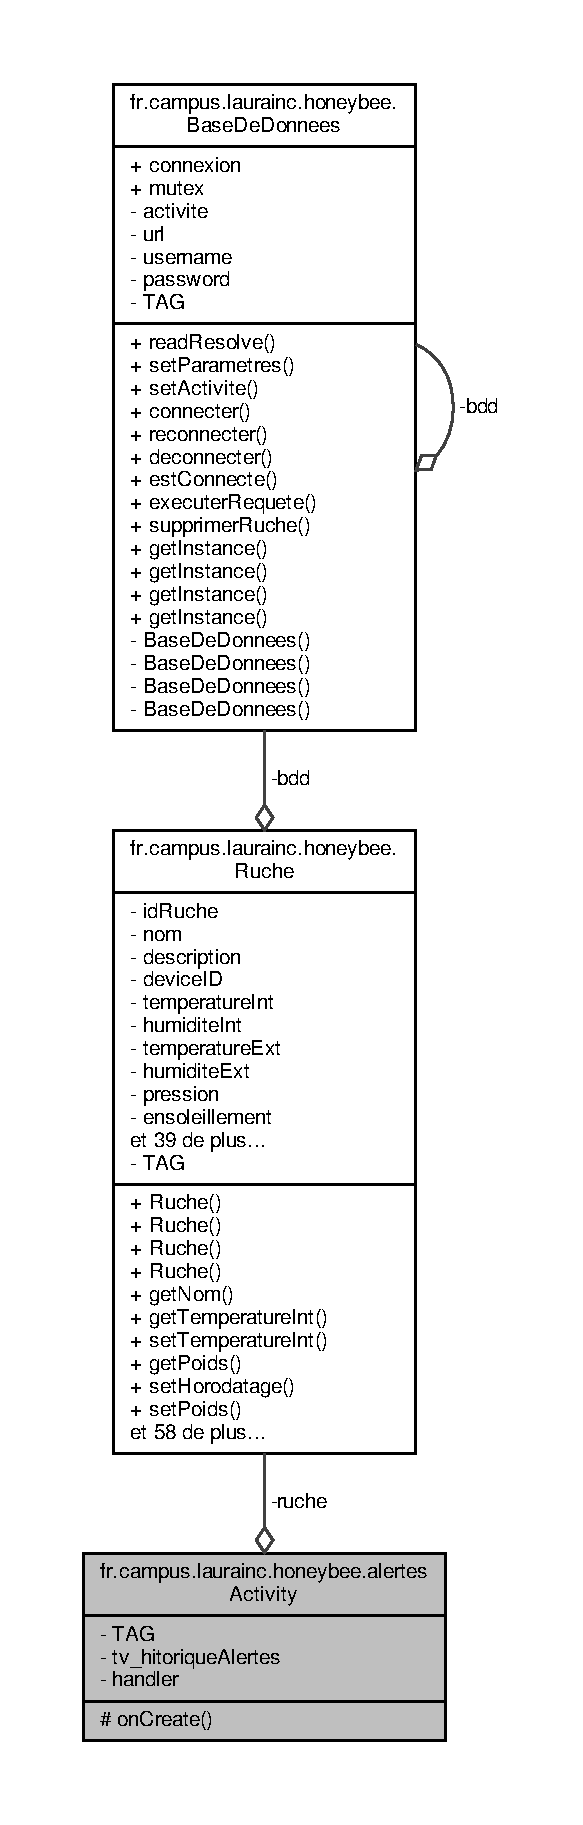
\includegraphics[height=550pt]{classfr_1_1campus_1_1laurainc_1_1honeybee_1_1alertes_activity__coll__graph}
\end{center}
\end{figure}
\subsubsection*{Fonctions membres protégées}
\begin{DoxyCompactItemize}
\item 
void \hyperlink{classfr_1_1campus_1_1laurainc_1_1honeybee_1_1alertes_activity_ade0f23cba3f8f4aaa65367baea096d88}{on\+Create} (Bundle saved\+Instance\+State)
\end{DoxyCompactItemize}
\subsubsection*{Attributs privés}
\begin{DoxyCompactItemize}
\item 
final String \hyperlink{classfr_1_1campus_1_1laurainc_1_1honeybee_1_1alertes_activity_af9b493032767c7ef4a5fa29d194e3bb3}{T\+AG} = \char`\"{}alertes\+Activity\char`\"{}
\item 
Text\+View \hyperlink{classfr_1_1campus_1_1laurainc_1_1honeybee_1_1alertes_activity_a957b9ea11ac3b17e5058cb91f93500e3}{tv\+\_\+hitorique\+Alertes}
\item 
\hyperlink{classfr_1_1campus_1_1laurainc_1_1honeybee_1_1_ruche}{Ruche} \hyperlink{classfr_1_1campus_1_1laurainc_1_1honeybee_1_1alertes_activity_a60ca5664100d5d388966a90342e7c93f}{ruche}
\item 
final Handler \hyperlink{classfr_1_1campus_1_1laurainc_1_1honeybee_1_1alertes_activity_a79cdc606c07f6f7655c8c6351be23785}{handler}
\end{DoxyCompactItemize}


\subsubsection{Documentation des fonctions membres}
\mbox{\Hypertarget{classfr_1_1campus_1_1laurainc_1_1honeybee_1_1alertes_activity_ade0f23cba3f8f4aaa65367baea096d88}\label{classfr_1_1campus_1_1laurainc_1_1honeybee_1_1alertes_activity_ade0f23cba3f8f4aaa65367baea096d88}} 
\index{fr\+::campus\+::laurainc\+::honeybee\+::alertes\+Activity@{fr\+::campus\+::laurainc\+::honeybee\+::alertes\+Activity}!on\+Create@{on\+Create}}
\index{on\+Create@{on\+Create}!fr\+::campus\+::laurainc\+::honeybee\+::alertes\+Activity@{fr\+::campus\+::laurainc\+::honeybee\+::alertes\+Activity}}
\paragraph{\texorpdfstring{on\+Create()}{onCreate()}}
{\footnotesize\ttfamily void fr.\+campus.\+laurainc.\+honeybee.\+alertes\+Activity.\+on\+Create (\begin{DoxyParamCaption}\item[{Bundle}]{saved\+Instance\+State }\end{DoxyParamCaption})\hspace{0.3cm}{\ttfamily [protected]}}



Références \hyperlink{classfr_1_1campus_1_1laurainc_1_1honeybee_1_1alertes_activity_a79cdc606c07f6f7655c8c6351be23785}{fr.\+campus.\+laurainc.\+honeybee.\+alertes\+Activity.\+handler}, et \hyperlink{classfr_1_1campus_1_1laurainc_1_1honeybee_1_1_ruche_ace10a52a470257f2b8f161fc3c7b9f15}{fr.\+campus.\+laurainc.\+honeybee.\+Ruche.\+recuperer\+Historique\+Alertes()}.


\begin{DoxyCode}
00017                                                        \{
00018         super.onCreate(savedInstanceState);
00019         setContentView(R.layout.activity\_alertes);
00020 
00021         \hyperlink{classfr_1_1campus_1_1laurainc_1_1honeybee_1_1alertes_activity_a60ca5664100d5d388966a90342e7c93f}{ruche} = \textcolor{keyword}{new} \hyperlink{class_ruche}{Ruche}(\hyperlink{classfr_1_1campus_1_1laurainc_1_1honeybee_1_1alertes_activity_a79cdc606c07f6f7655c8c6351be23785}{handler});
00022 
00023         \hyperlink{classfr_1_1campus_1_1laurainc_1_1honeybee_1_1alertes_activity_a957b9ea11ac3b17e5058cb91f93500e3}{tv\_hitoriqueAlertes} = findViewById(R.id.tv\_historiqueAlertes);
00024         \hyperlink{classfr_1_1campus_1_1laurainc_1_1honeybee_1_1alertes_activity_a60ca5664100d5d388966a90342e7c93f}{ruche}.\hyperlink{classfr_1_1campus_1_1laurainc_1_1honeybee_1_1_ruche_ace10a52a470257f2b8f161fc3c7b9f15}{recupererHistoriqueAlertes}();
00025 
00026     \}
\end{DoxyCode}


\subsubsection{Documentation des données membres}
\mbox{\Hypertarget{classfr_1_1campus_1_1laurainc_1_1honeybee_1_1alertes_activity_a79cdc606c07f6f7655c8c6351be23785}\label{classfr_1_1campus_1_1laurainc_1_1honeybee_1_1alertes_activity_a79cdc606c07f6f7655c8c6351be23785}} 
\index{fr\+::campus\+::laurainc\+::honeybee\+::alertes\+Activity@{fr\+::campus\+::laurainc\+::honeybee\+::alertes\+Activity}!handler@{handler}}
\index{handler@{handler}!fr\+::campus\+::laurainc\+::honeybee\+::alertes\+Activity@{fr\+::campus\+::laurainc\+::honeybee\+::alertes\+Activity}}
\paragraph{\texorpdfstring{handler}{handler}}
{\footnotesize\ttfamily final Handler fr.\+campus.\+laurainc.\+honeybee.\+alertes\+Activity.\+handler\hspace{0.3cm}{\ttfamily [private]}}

{\bfseries Valeur initiale \+:}
\begin{DoxyCode}
= \textcolor{keyword}{new} Handler()
    \{
        
        \textcolor{keyword}{public} \textcolor{keywordtype}{void} handleMessage(Message msg)
        \{
            super.handleMessage(msg);
            \textcolor{keywordflow}{switch} (msg.what)
            \{
                \textcolor{keywordflow}{case} HoneyBee.REQUETE\_SQL\_ERREUR:
                    Log.d(\hyperlink{classfr_1_1campus_1_1laurainc_1_1honeybee_1_1alertes_activity_af9b493032767c7ef4a5fa29d194e3bb3}{TAG}, \textcolor{stringliteral}{"handleMessage -> REQUETE SQL ERREUR"});
                    \textcolor{keywordflow}{break};
                \textcolor{keywordflow}{case} HoneyBee.REQUETE\_SQL\_ALERTES:
                    Log.d(\hyperlink{classfr_1_1campus_1_1laurainc_1_1honeybee_1_1alertes_activity_af9b493032767c7ef4a5fa29d194e3bb3}{TAG}, \textcolor{stringliteral}{"handleMessage -> REQUETE SQL ALERTES"});
                    \hyperlink{classfr_1_1campus_1_1laurainc_1_1honeybee_1_1alertes_activity_a957b9ea11ac3b17e5058cb91f93500e3}{tv\_hitoriqueAlertes}.setText(\hyperlink{classfr_1_1campus_1_1laurainc_1_1honeybee_1_1alertes_activity_a60ca5664100d5d388966a90342e7c93f}{ruche}.
      \hyperlink{classfr_1_1campus_1_1laurainc_1_1honeybee_1_1_ruche_a97cc64f6d39ee995175e389bad662b86}{getHistoriqueAlertes}());
                    \textcolor{keywordflow}{break};
            \}
        \}
    \}
\end{DoxyCode}


Référencé par \hyperlink{classfr_1_1campus_1_1laurainc_1_1honeybee_1_1alertes_activity_ade0f23cba3f8f4aaa65367baea096d88}{fr.\+campus.\+laurainc.\+honeybee.\+alertes\+Activity.\+on\+Create()}.

\mbox{\Hypertarget{classfr_1_1campus_1_1laurainc_1_1honeybee_1_1alertes_activity_a60ca5664100d5d388966a90342e7c93f}\label{classfr_1_1campus_1_1laurainc_1_1honeybee_1_1alertes_activity_a60ca5664100d5d388966a90342e7c93f}} 
\index{fr\+::campus\+::laurainc\+::honeybee\+::alertes\+Activity@{fr\+::campus\+::laurainc\+::honeybee\+::alertes\+Activity}!ruche@{ruche}}
\index{ruche@{ruche}!fr\+::campus\+::laurainc\+::honeybee\+::alertes\+Activity@{fr\+::campus\+::laurainc\+::honeybee\+::alertes\+Activity}}
\paragraph{\texorpdfstring{ruche}{ruche}}
{\footnotesize\ttfamily \hyperlink{classfr_1_1campus_1_1laurainc_1_1honeybee_1_1_ruche}{Ruche} fr.\+campus.\+laurainc.\+honeybee.\+alertes\+Activity.\+ruche\hspace{0.3cm}{\ttfamily [private]}}

\mbox{\Hypertarget{classfr_1_1campus_1_1laurainc_1_1honeybee_1_1alertes_activity_af9b493032767c7ef4a5fa29d194e3bb3}\label{classfr_1_1campus_1_1laurainc_1_1honeybee_1_1alertes_activity_af9b493032767c7ef4a5fa29d194e3bb3}} 
\index{fr\+::campus\+::laurainc\+::honeybee\+::alertes\+Activity@{fr\+::campus\+::laurainc\+::honeybee\+::alertes\+Activity}!T\+AG@{T\+AG}}
\index{T\+AG@{T\+AG}!fr\+::campus\+::laurainc\+::honeybee\+::alertes\+Activity@{fr\+::campus\+::laurainc\+::honeybee\+::alertes\+Activity}}
\paragraph{\texorpdfstring{T\+AG}{TAG}}
{\footnotesize\ttfamily final String fr.\+campus.\+laurainc.\+honeybee.\+alertes\+Activity.\+T\+AG = \char`\"{}alertes\+Activity\char`\"{}\hspace{0.3cm}{\ttfamily [private]}}

\mbox{\Hypertarget{classfr_1_1campus_1_1laurainc_1_1honeybee_1_1alertes_activity_a957b9ea11ac3b17e5058cb91f93500e3}\label{classfr_1_1campus_1_1laurainc_1_1honeybee_1_1alertes_activity_a957b9ea11ac3b17e5058cb91f93500e3}} 
\index{fr\+::campus\+::laurainc\+::honeybee\+::alertes\+Activity@{fr\+::campus\+::laurainc\+::honeybee\+::alertes\+Activity}!tv\+\_\+hitorique\+Alertes@{tv\+\_\+hitorique\+Alertes}}
\index{tv\+\_\+hitorique\+Alertes@{tv\+\_\+hitorique\+Alertes}!fr\+::campus\+::laurainc\+::honeybee\+::alertes\+Activity@{fr\+::campus\+::laurainc\+::honeybee\+::alertes\+Activity}}
\paragraph{\texorpdfstring{tv\+\_\+hitorique\+Alertes}{tv\_hitoriqueAlertes}}
{\footnotesize\ttfamily Text\+View fr.\+campus.\+laurainc.\+honeybee.\+alertes\+Activity.\+tv\+\_\+hitorique\+Alertes\hspace{0.3cm}{\ttfamily [private]}}



La documentation de cette classe a été générée à partir du fichier suivant \+:\begin{DoxyCompactItemize}
\item 
\hyperlink{alertes_activity_8java}{alertes\+Activity.\+java}\end{DoxyCompactItemize}

\hypertarget{class_base_de_donnees}{}\subsection{Référence de la classe Base\+De\+Donnees}
\label{class_base_de_donnees}\index{Base\+De\+Donnees@{Base\+De\+Donnees}}


{\ttfamily \#include $<$base\+De\+Donnees.\+h$>$}



Graphe de collaboration de Base\+De\+Donnees\+:\nopagebreak
\begin{figure}[H]
\begin{center}
\leavevmode
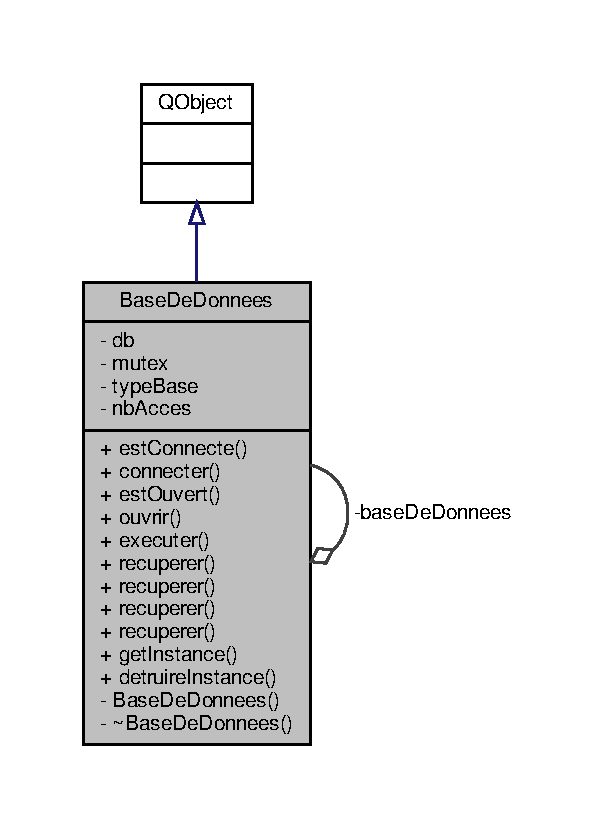
\includegraphics[width=286pt]{class_base_de_donnees__coll__graph}
\end{center}
\end{figure}
\subsubsection*{Fonctions membres publiques}
\begin{DoxyCompactItemize}
\item 
bool \hyperlink{class_base_de_donnees_a00388973f3ec42e5c8e76e7af7e124b2}{est\+Connecte} ()
\item 
bool \hyperlink{class_base_de_donnees_ac20da193923a9bfea5e38ee5a54820cd}{connecter} (Q\+String nom\+Base=\hyperlink{parametres_8h_a45f8f15b8f9a7ab4c2b219038ff64f6b}{B\+D\+D\+\_\+\+N\+O\+M\+B\+A\+SE}, Q\+String username=\hyperlink{parametres_8h_a88b5f5b81fa534553c68802384beff2c}{B\+D\+D\+\_\+\+U\+S\+E\+R\+N\+A\+ME}, Q\+String password=\hyperlink{parametres_8h_ae2ded9166ed2553182545e97514c04f7}{B\+D\+D\+\_\+\+P\+A\+S\+S\+W\+O\+RD}, Q\+String serveur=\hyperlink{parametres_8h_a423559dc987673b8aacaa9f369839bb0}{B\+D\+D\+\_\+\+S\+E\+R\+V\+E\+UR})
\item 
bool \hyperlink{class_base_de_donnees_af9ac332082ffd0dd35e412cefabe5e9c}{est\+Ouvert} ()
\item 
bool \hyperlink{class_base_de_donnees_a7f6a5510b08017b0d99115a84252f186}{ouvrir} (Q\+String fichier\+Base)
\item 
bool \hyperlink{class_base_de_donnees_aa8de5f8f8bb17edc43f5c0ee33712081}{executer} (Q\+String requete)
\item 
bool \hyperlink{class_base_de_donnees_a77539baad389f5acf754cd2cd452403e}{recuperer} (Q\+String requete, Q\+String \&donnees)
\item 
bool \hyperlink{class_base_de_donnees_a2a5c461fa11d404810ae3ebe035d5190}{recuperer} (Q\+String requete, Q\+String\+List \&donnees)
\item 
bool \hyperlink{class_base_de_donnees_af9a76eb2b12df784280c379a4b22af62}{recuperer} (Q\+String requete, Q\+Vector$<$ Q\+String $>$ \&donnees)
\item 
bool \hyperlink{class_base_de_donnees_a68dd0d62ba03b9e8e5aa759d0666cb59}{recuperer} (Q\+String requete, Q\+Vector$<$ Q\+String\+List $>$ \&donnees)
\end{DoxyCompactItemize}
\subsubsection*{Fonctions membres publiques statiques}
\begin{DoxyCompactItemize}
\item 
static \hyperlink{class_base_de_donnees}{Base\+De\+Donnees} $\ast$ \hyperlink{class_base_de_donnees_a80028aa2b6b4fbf30fb2e36357b7d3d3}{get\+Instance} (Q\+String type=\char`\"{}Q\+M\+Y\+S\+QL\char`\"{})
\item 
static void \hyperlink{class_base_de_donnees_a457401c0816b888c77ce915997545f4e}{detruire\+Instance} ()
\end{DoxyCompactItemize}
\subsubsection*{Fonctions membres privées}
\begin{DoxyCompactItemize}
\item 
\hyperlink{class_base_de_donnees_a10dd177f1008f675ab78c2221b2a6750}{Base\+De\+Donnees} (Q\+String type)
\item 
\hyperlink{class_base_de_donnees_a5dc474cdbe003644fb0ca7b8f2ec6b93}{$\sim$\+Base\+De\+Donnees} ()
\end{DoxyCompactItemize}
\subsubsection*{Attributs privés}
\begin{DoxyCompactItemize}
\item 
Q\+Sql\+Database \hyperlink{class_base_de_donnees_a3e738dcf443370c46a541677ab619f06}{db}
\item 
Q\+Mutex \hyperlink{class_base_de_donnees_aa1b4696fac87a740f914aa73739086f2}{mutex}
\end{DoxyCompactItemize}
\subsubsection*{Attributs privés statiques}
\begin{DoxyCompactItemize}
\item 
static \hyperlink{class_base_de_donnees}{Base\+De\+Donnees} $\ast$ \hyperlink{class_base_de_donnees_a822ba0b7cf85b1e48ced8efd3d65e266}{base\+De\+Donnees} = N\+U\+LL
\item 
static Q\+String \hyperlink{class_base_de_donnees_ab682b82167f494496a6531bfe522b42b}{type\+Base} = \char`\"{}Q\+M\+Y\+S\+QL\char`\"{}
\item 
static int \hyperlink{class_base_de_donnees_a5099ecb2922bb31d84cd5d4505298a29}{nb\+Acces} = 0
\end{DoxyCompactItemize}


\subsubsection{Documentation des constructeurs et destructeur}
\mbox{\Hypertarget{class_base_de_donnees_a10dd177f1008f675ab78c2221b2a6750}\label{class_base_de_donnees_a10dd177f1008f675ab78c2221b2a6750}} 
\index{Base\+De\+Donnees@{Base\+De\+Donnees}!Base\+De\+Donnees@{Base\+De\+Donnees}}
\index{Base\+De\+Donnees@{Base\+De\+Donnees}!Base\+De\+Donnees@{Base\+De\+Donnees}}
\paragraph{\texorpdfstring{Base\+De\+Donnees()}{BaseDeDonnees()}}
{\footnotesize\ttfamily Base\+De\+Donnees\+::\+Base\+De\+Donnees (\begin{DoxyParamCaption}\item[{Q\+String}]{type }\end{DoxyParamCaption})\hspace{0.3cm}{\ttfamily [private]}}



Références \hyperlink{class_base_de_donnees_a3e738dcf443370c46a541677ab619f06}{db}, et \hyperlink{class_base_de_donnees_ab682b82167f494496a6531bfe522b42b}{type\+Base}.



Référencé par \hyperlink{class_base_de_donnees_a80028aa2b6b4fbf30fb2e36357b7d3d3}{get\+Instance()}.


\begin{DoxyCode}
00023 \{
00024 \textcolor{preprocessor}{    #ifdef DEBUG\_BASEDEDONNEES}
00025     qDebug() << Q\_FUNC\_INFO << type;
00026 \textcolor{preprocessor}{    #endif}
00027     \hyperlink{class_base_de_donnees_a3e738dcf443370c46a541677ab619f06}{db} = QSqlDatabase::addDatabase(type);
00028     \hyperlink{class_base_de_donnees_ab682b82167f494496a6531bfe522b42b}{typeBase} = type;
00029 \}
\end{DoxyCode}
\mbox{\Hypertarget{class_base_de_donnees_a5dc474cdbe003644fb0ca7b8f2ec6b93}\label{class_base_de_donnees_a5dc474cdbe003644fb0ca7b8f2ec6b93}} 
\index{Base\+De\+Donnees@{Base\+De\+Donnees}!````~Base\+De\+Donnees@{$\sim$\+Base\+De\+Donnees}}
\index{````~Base\+De\+Donnees@{$\sim$\+Base\+De\+Donnees}!Base\+De\+Donnees@{Base\+De\+Donnees}}
\paragraph{\texorpdfstring{$\sim$\+Base\+De\+Donnees()}{~BaseDeDonnees()}}
{\footnotesize\ttfamily Base\+De\+Donnees\+::$\sim$\+Base\+De\+Donnees (\begin{DoxyParamCaption}{ }\end{DoxyParamCaption})\hspace{0.3cm}{\ttfamily [private]}}


\begin{DoxyCode}
00032 \{
00033 \textcolor{preprocessor}{    #ifdef DEBUG\_BASEDEDONNEES}
00034     qDebug() << Q\_FUNC\_INFO;
00035 \textcolor{preprocessor}{    #endif}
00036 \}
\end{DoxyCode}


\subsubsection{Documentation des fonctions membres}
\mbox{\Hypertarget{class_base_de_donnees_ac20da193923a9bfea5e38ee5a54820cd}\label{class_base_de_donnees_ac20da193923a9bfea5e38ee5a54820cd}} 
\index{Base\+De\+Donnees@{Base\+De\+Donnees}!connecter@{connecter}}
\index{connecter@{connecter}!Base\+De\+Donnees@{Base\+De\+Donnees}}
\paragraph{\texorpdfstring{connecter()}{connecter()}}
{\footnotesize\ttfamily bool Base\+De\+Donnees\+::connecter (\begin{DoxyParamCaption}\item[{Q\+String}]{nom\+Base = {\ttfamily \hyperlink{parametres_8h_a45f8f15b8f9a7ab4c2b219038ff64f6b}{B\+D\+D\+\_\+\+N\+O\+M\+B\+A\+SE}},  }\item[{Q\+String}]{username = {\ttfamily \hyperlink{parametres_8h_a88b5f5b81fa534553c68802384beff2c}{B\+D\+D\+\_\+\+U\+S\+E\+R\+N\+A\+ME}},  }\item[{Q\+String}]{password = {\ttfamily \hyperlink{parametres_8h_ae2ded9166ed2553182545e97514c04f7}{B\+D\+D\+\_\+\+P\+A\+S\+S\+W\+O\+RD}},  }\item[{Q\+String}]{serveur = {\ttfamily \hyperlink{parametres_8h_a423559dc987673b8aacaa9f369839bb0}{B\+D\+D\+\_\+\+S\+E\+R\+V\+E\+UR}} }\end{DoxyParamCaption})}



Références \hyperlink{parametres_8h_ace364d1ce44aa9f79bcff6e3752c4a5f}{A\+P\+P\+\_\+\+T\+I\+T\+RE}, \hyperlink{class_base_de_donnees_a3e738dcf443370c46a541677ab619f06}{db}, \hyperlink{class_base_de_donnees_aa1b4696fac87a740f914aa73739086f2}{mutex}, et \hyperlink{class_base_de_donnees_ab682b82167f494496a6531bfe522b42b}{type\+Base}.



Référencé par \hyperlink{class_alertes_ad2e4e3907f97bdd06840dfeee0a87ddb}{Alertes\+::\+Alertes()}, \hyperlink{class_nouvelle_ruche_ihm_a338b9af0b96ed0839a8d5008c8c89cc4}{Nouvelle\+Ruche\+Ihm\+::\+Nouvelle\+Ruche\+Ihm()}, \hyperlink{class_reglages_alertes_ihm_ae6337f2d05a3184e48bf5022a91f06c7}{Reglages\+Alertes\+Ihm\+::\+Reglages\+Alertes\+Ihm()}, \hyperlink{class_ruche_a8b4ee3752d984c5acee93b990db7939a}{Ruche\+::\+Ruche()}, et \hyperlink{class_ruche_ihm_a04c2544ba4e9cca6c38f553c32d63dee}{Ruche\+Ihm\+::\+Ruche\+Ihm()}.


\begin{DoxyCode}
00077 \{
00078     \textcolor{keywordflow}{if}(\hyperlink{class_base_de_donnees_ab682b82167f494496a6531bfe522b42b}{typeBase} != \textcolor{stringliteral}{"QMYSQL"})
00079         \textcolor{keywordflow}{return} \textcolor{keyword}{false};
00080     QMutexLocker verrou(&\hyperlink{class_base_de_donnees_aa1b4696fac87a740f914aa73739086f2}{mutex});
00081     \textcolor{keywordflow}{if}(!\hyperlink{class_base_de_donnees_a3e738dcf443370c46a541677ab619f06}{db}.isOpen())
00082     \{
00083        \hyperlink{class_base_de_donnees_a3e738dcf443370c46a541677ab619f06}{db}.setHostName(serveur);
00084        \hyperlink{class_base_de_donnees_a3e738dcf443370c46a541677ab619f06}{db}.setUserName(username);
00085        \hyperlink{class_base_de_donnees_a3e738dcf443370c46a541677ab619f06}{db}.setPassword(password);
00086        \hyperlink{class_base_de_donnees_a3e738dcf443370c46a541677ab619f06}{db}.setDatabaseName(nomBase);
00087 
00088 \textcolor{preprocessor}{       #ifdef DEBUG\_BASEDEDONNEES}
00089        qDebug() << Q\_FUNC\_INFO;
00090        qDebug() << \textcolor{stringliteral}{"HostName : "} << \hyperlink{class_base_de_donnees_a3e738dcf443370c46a541677ab619f06}{db}.hostName();
00091        qDebug() << \textcolor{stringliteral}{"UserName : "} << \hyperlink{class_base_de_donnees_a3e738dcf443370c46a541677ab619f06}{db}.userName();
00092        qDebug() << \textcolor{stringliteral}{"DatabaseName : "} << \hyperlink{class_base_de_donnees_a3e738dcf443370c46a541677ab619f06}{db}.databaseName();
00093 \textcolor{preprocessor}{       #endif}
00094        \textcolor{keywordflow}{if}(\hyperlink{class_base_de_donnees_a3e738dcf443370c46a541677ab619f06}{db}.open())
00095        \{
00096 \textcolor{preprocessor}{           #ifdef DEBUG\_BASEDEDONNEES}
00097            qDebug() << Q\_FUNC\_INFO << QString::fromUtf8(\textcolor{stringliteral}{"Connexion réussie à %1"}).arg(
      \hyperlink{class_base_de_donnees_a3e738dcf443370c46a541677ab619f06}{db}.hostName());
00098 \textcolor{preprocessor}{           #endif}
00099            \textcolor{keywordflow}{return} \textcolor{keyword}{true};
00100        \}
00101        \textcolor{keywordflow}{else}
00102        \{
00103            qDebug() << Q\_FUNC\_INFO << QString::fromUtf8(\textcolor{stringliteral}{"Erreur : impossible de se connecter à la base de
       données !"});
00104            QMessageBox::critical(0, QString::fromUtf8(\hyperlink{parametres_8h_ace364d1ce44aa9f79bcff6e3752c4a5f}{APP\_TITRE}), QString::fromUtf8(\textcolor{stringliteral}{"Impossible de
       se connecter à la base de données !"}));
00105            \textcolor{keywordflow}{return} \textcolor{keyword}{false};
00106        \}
00107     \}
00108     \textcolor{keywordflow}{else}
00109         \textcolor{keywordflow}{return} \textcolor{keyword}{true};
00110 \}
\end{DoxyCode}
\mbox{\Hypertarget{class_base_de_donnees_a457401c0816b888c77ce915997545f4e}\label{class_base_de_donnees_a457401c0816b888c77ce915997545f4e}} 
\index{Base\+De\+Donnees@{Base\+De\+Donnees}!detruire\+Instance@{detruire\+Instance}}
\index{detruire\+Instance@{detruire\+Instance}!Base\+De\+Donnees@{Base\+De\+Donnees}}
\paragraph{\texorpdfstring{detruire\+Instance()}{detruireInstance()}}
{\footnotesize\ttfamily void Base\+De\+Donnees\+::detruire\+Instance (\begin{DoxyParamCaption}{ }\end{DoxyParamCaption})\hspace{0.3cm}{\ttfamily [static]}}



Références \hyperlink{class_base_de_donnees_a822ba0b7cf85b1e48ced8efd3d65e266}{base\+De\+Donnees}, et \hyperlink{class_base_de_donnees_a5099ecb2922bb31d84cd5d4505298a29}{nb\+Acces}.



Référencé par \hyperlink{class_alertes_a730b10861d04de9944b30b11c6b3c3af}{Alertes\+::$\sim$\+Alertes()}, \hyperlink{class_nouvelle_ruche_ihm_a17e5dfd1146574134eaa3ab8eae4f6d4}{Nouvelle\+Ruche\+Ihm\+::$\sim$\+Nouvelle\+Ruche\+Ihm()}, \hyperlink{class_reglages_alertes_ihm_aa9bfc09b4162f536de84d218daa36982}{Reglages\+Alertes\+Ihm\+::$\sim$\+Reglages\+Alertes\+Ihm()}, \hyperlink{class_ruche_ad3f950d0731f9801f06dd6ae09f2e5fa}{Ruche\+::$\sim$\+Ruche()}, et \hyperlink{class_ruche_ihm_a4c489bf18e8c9947a375322d03504419}{Ruche\+Ihm\+::$\sim$\+Ruche\+Ihm()}.


\begin{DoxyCode}
00052 \{
00053     \textcolor{comment}{// instance ?}
00054     \textcolor{keywordflow}{if}(\hyperlink{class_base_de_donnees_a822ba0b7cf85b1e48ced8efd3d65e266}{baseDeDonnees} != NULL)
00055     \{
00056         \textcolor{keywordflow}{if}(\hyperlink{class_base_de_donnees_a5099ecb2922bb31d84cd5d4505298a29}{nbAcces} > 0)
00057             \hyperlink{class_base_de_donnees_a5099ecb2922bb31d84cd5d4505298a29}{nbAcces}--;
00058 \textcolor{preprocessor}{        #ifdef DEBUG\_BASEDEDONNEES}
00059         qDebug() << Q\_FUNC\_INFO << \textcolor{stringliteral}{"nbAcces restants"} << \hyperlink{class_base_de_donnees_a5099ecb2922bb31d84cd5d4505298a29}{nbAcces};
00060 \textcolor{preprocessor}{        #endif}
00061         \textcolor{comment}{// dernier ?}
00062         \textcolor{keywordflow}{if}(nbAcces == 0)
00063         \{
00064             \textcolor{keyword}{delete} \hyperlink{class_base_de_donnees_a822ba0b7cf85b1e48ced8efd3d65e266}{baseDeDonnees};
00065             \hyperlink{class_base_de_donnees_a822ba0b7cf85b1e48ced8efd3d65e266}{baseDeDonnees} = NULL;
00066         \}
00067     \}
00068 \}
\end{DoxyCode}
\mbox{\Hypertarget{class_base_de_donnees_a00388973f3ec42e5c8e76e7af7e124b2}\label{class_base_de_donnees_a00388973f3ec42e5c8e76e7af7e124b2}} 
\index{Base\+De\+Donnees@{Base\+De\+Donnees}!est\+Connecte@{est\+Connecte}}
\index{est\+Connecte@{est\+Connecte}!Base\+De\+Donnees@{Base\+De\+Donnees}}
\paragraph{\texorpdfstring{est\+Connecte()}{estConnecte()}}
{\footnotesize\ttfamily bool Base\+De\+Donnees\+::est\+Connecte (\begin{DoxyParamCaption}{ }\end{DoxyParamCaption})}



Références \hyperlink{class_base_de_donnees_a3e738dcf443370c46a541677ab619f06}{db}, et \hyperlink{class_base_de_donnees_aa1b4696fac87a740f914aa73739086f2}{mutex}.



Référencé par \hyperlink{class_alertes_ad2e4e3907f97bdd06840dfeee0a87ddb}{Alertes\+::\+Alertes()}, \hyperlink{class_nouvelle_ruche_ihm_a338b9af0b96ed0839a8d5008c8c89cc4}{Nouvelle\+Ruche\+Ihm\+::\+Nouvelle\+Ruche\+Ihm()}, \hyperlink{class_reglages_alertes_ihm_ae6337f2d05a3184e48bf5022a91f06c7}{Reglages\+Alertes\+Ihm\+::\+Reglages\+Alertes\+Ihm()}, \hyperlink{class_ruche_a8b4ee3752d984c5acee93b990db7939a}{Ruche\+::\+Ruche()}, et \hyperlink{class_ruche_ihm_a04c2544ba4e9cca6c38f553c32d63dee}{Ruche\+Ihm\+::\+Ruche\+Ihm()}.


\begin{DoxyCode}
00071 \{
00072     QMutexLocker verrou(&\hyperlink{class_base_de_donnees_aa1b4696fac87a740f914aa73739086f2}{mutex});
00073     \textcolor{keywordflow}{return} \hyperlink{class_base_de_donnees_a3e738dcf443370c46a541677ab619f06}{db}.isOpen();
00074 \}
\end{DoxyCode}
\mbox{\Hypertarget{class_base_de_donnees_af9ac332082ffd0dd35e412cefabe5e9c}\label{class_base_de_donnees_af9ac332082ffd0dd35e412cefabe5e9c}} 
\index{Base\+De\+Donnees@{Base\+De\+Donnees}!est\+Ouvert@{est\+Ouvert}}
\index{est\+Ouvert@{est\+Ouvert}!Base\+De\+Donnees@{Base\+De\+Donnees}}
\paragraph{\texorpdfstring{est\+Ouvert()}{estOuvert()}}
{\footnotesize\ttfamily bool Base\+De\+Donnees\+::est\+Ouvert (\begin{DoxyParamCaption}{ }\end{DoxyParamCaption})}



Références \hyperlink{class_base_de_donnees_a3e738dcf443370c46a541677ab619f06}{db}, et \hyperlink{class_base_de_donnees_aa1b4696fac87a740f914aa73739086f2}{mutex}.


\begin{DoxyCode}
00113 \{
00114     QMutexLocker verrou(&\hyperlink{class_base_de_donnees_aa1b4696fac87a740f914aa73739086f2}{mutex});
00115     \textcolor{keywordflow}{return} \hyperlink{class_base_de_donnees_a3e738dcf443370c46a541677ab619f06}{db}.isOpen();
00116 \}
\end{DoxyCode}
\mbox{\Hypertarget{class_base_de_donnees_aa8de5f8f8bb17edc43f5c0ee33712081}\label{class_base_de_donnees_aa8de5f8f8bb17edc43f5c0ee33712081}} 
\index{Base\+De\+Donnees@{Base\+De\+Donnees}!executer@{executer}}
\index{executer@{executer}!Base\+De\+Donnees@{Base\+De\+Donnees}}
\paragraph{\texorpdfstring{executer()}{executer()}}
{\footnotesize\ttfamily bool Base\+De\+Donnees\+::executer (\begin{DoxyParamCaption}\item[{Q\+String}]{requete }\end{DoxyParamCaption})}



Références \hyperlink{class_base_de_donnees_a3e738dcf443370c46a541677ab619f06}{db}, et \hyperlink{class_base_de_donnees_aa1b4696fac87a740f914aa73739086f2}{mutex}.



Référencé par \hyperlink{class_ruche_ihm_a5181062e21dc73908b660d97e9621fb6}{Ruche\+Ihm\+::afficher\+Alertes\+Batterie()}, \hyperlink{class_ruche_ihm_aea5efc506f9825db2a4eb39a40d7eb18}{Ruche\+Ihm\+::afficher\+Alertes\+Ensoleillement()}, \hyperlink{class_ruche_ihm_a76b73e39e55443fc7b9bb773eac3321f}{Ruche\+Ihm\+::afficher\+Alertes\+Humidite\+Exterieur()}, \hyperlink{class_ruche_ihm_abfe91b271dde97048bb218b04c9e167b}{Ruche\+Ihm\+::afficher\+Alertes\+Humidite\+Interieur()}, \hyperlink{class_ruche_ihm_a641d05346e527c3386ed9df6a7e6fafc}{Ruche\+Ihm\+::afficher\+Alertes\+Poids()}, \hyperlink{class_ruche_ihm_abea08b19d4f52f6767a8618bbc25d956}{Ruche\+Ihm\+::afficher\+Alertes\+Pression\+Atmospherique()}, \hyperlink{class_ruche_ihm_ada4be5a54f7fa57de6190d44e3cfcb82}{Ruche\+Ihm\+::afficher\+Alertes\+Temperature\+Exterieur()}, \hyperlink{class_ruche_ihm_af4848134f2bc17d9772f2408a068e9d8}{Ruche\+Ihm\+::afficher\+Alertes\+Temperature\+Interieur()}, \hyperlink{class_ruche_a509367d6b2bcb7e6431fc1cc5ff606b5}{Ruche\+::inserer\+Donnees\+Port\+Batterie()}, \hyperlink{class_ruche_ad21de5f7d48195be0658f52c55f34183}{Ruche\+::inserer\+Donnees\+Port\+Ensoleillement()}, \hyperlink{class_ruche_a46c0f440f40a5125f2d579b481660457}{Ruche\+::inserer\+Donnees\+Port\+Mesure\+Environnement()}, \hyperlink{class_ruche_aa61f6dd8b15e5242ef3a3bdd87cca4a3}{Ruche\+::inserer\+Donnees\+Port\+Mesure\+Ruche()}, \hyperlink{class_ruche_a923f42fc4878a01f6102966a748e8f37}{Ruche\+::inserer\+Donnees\+Port\+Poids()}, \hyperlink{class_ruche_a658234b9d96541d204b95b74556742b6}{Ruche\+::inserer\+Mesure\+Horaire\+Ensoleillement()}, \hyperlink{class_ruche_ac52e79446c5629645e02e27d2a01e56c}{Ruche\+::inserer\+Mesure\+Horaire\+Environnement()}, \hyperlink{class_ruche_a3a093c088d9c97f347394c8a681f7302}{Ruche\+::inserer\+Mesure\+Horaire\+Ruche()}, \hyperlink{class_nouvelle_ruche_ihm_a268e781b033f2531ca5eab19cc828fdc}{Nouvelle\+Ruche\+Ihm\+::recevoir\+Donnee\+Ajout\+Ruche()}, \hyperlink{class_reglages_alertes_ihm_a5c40f718b28b948a90574ef0c2d3e587}{Reglages\+Alertes\+Ihm\+::recevoir\+Reglages\+Alertes()}, et \hyperlink{class_ruche_ihm_a85729b1ae4f3dfb5130eb45f5a426e3c}{Ruche\+Ihm\+::supprimer\+Ruche()}.


\begin{DoxyCode}
00151 \{
00152     QMutexLocker verrou(&\hyperlink{class_base_de_donnees_aa1b4696fac87a740f914aa73739086f2}{mutex});
00153     QSqlQuery r;
00154     \textcolor{keywordtype}{bool} retour;
00155 
00156     \textcolor{keywordflow}{if}(\hyperlink{class_base_de_donnees_a3e738dcf443370c46a541677ab619f06}{db}.isOpen())
00157     \{
00158         \textcolor{keywordflow}{if}(requete.contains(\textcolor{stringliteral}{"UPDATE"}) || requete.contains(\textcolor{stringliteral}{"INSERT"}) || requete.contains(\textcolor{stringliteral}{"DELETE"}))
00159         \{
00160             retour = r.exec(requete);
00161 \textcolor{preprocessor}{            #ifdef DEBUG\_BASEDEDONNEES}
00162             qDebug() << Q\_FUNC\_INFO << QString::fromUtf8(\textcolor{stringliteral}{"Retour %1 pour la requete : %2"}).arg(
      QString::number(retour)).arg(requete);
00163 \textcolor{preprocessor}{            #endif}
00164             \textcolor{keywordflow}{if}(retour)
00165             \{
00166                 \textcolor{keywordflow}{return} \textcolor{keyword}{true};
00167             \}
00168             \textcolor{keywordflow}{else}
00169             \{
00170                 qDebug() << Q\_FUNC\_INFO << QString::fromUtf8(\textcolor{stringliteral}{"Erreur : %1 pour la requête %2"}).arg(r.
      lastError().text()).arg(requete);
00171                 \textcolor{keywordflow}{return} \textcolor{keyword}{false};
00172             \}
00173         \}
00174         \textcolor{keywordflow}{else}
00175         \{
00176             qDebug() << Q\_FUNC\_INFO << QString::fromUtf8(\textcolor{stringliteral}{"Erreur : requête %1 non autorisée !"}).arg(requete
      );
00177             \textcolor{keywordflow}{return} \textcolor{keyword}{false};
00178         \}
00179     \}
00180     \textcolor{keywordflow}{else}
00181         \textcolor{keywordflow}{return} \textcolor{keyword}{false};
00182 
00183 \}
\end{DoxyCode}
\mbox{\Hypertarget{class_base_de_donnees_a80028aa2b6b4fbf30fb2e36357b7d3d3}\label{class_base_de_donnees_a80028aa2b6b4fbf30fb2e36357b7d3d3}} 
\index{Base\+De\+Donnees@{Base\+De\+Donnees}!get\+Instance@{get\+Instance}}
\index{get\+Instance@{get\+Instance}!Base\+De\+Donnees@{Base\+De\+Donnees}}
\paragraph{\texorpdfstring{get\+Instance()}{getInstance()}}
{\footnotesize\ttfamily \hyperlink{class_base_de_donnees}{Base\+De\+Donnees} $\ast$ Base\+De\+Donnees\+::get\+Instance (\begin{DoxyParamCaption}\item[{Q\+String}]{type = {\ttfamily \char`\"{}QMYSQL\char`\"{}} }\end{DoxyParamCaption})\hspace{0.3cm}{\ttfamily [static]}}



Références \hyperlink{class_base_de_donnees_a10dd177f1008f675ab78c2221b2a6750}{Base\+De\+Donnees()}, \hyperlink{class_base_de_donnees_a822ba0b7cf85b1e48ced8efd3d65e266}{base\+De\+Donnees}, et \hyperlink{class_base_de_donnees_a5099ecb2922bb31d84cd5d4505298a29}{nb\+Acces}.



Référencé par \hyperlink{class_alertes_ad2e4e3907f97bdd06840dfeee0a87ddb}{Alertes\+::\+Alertes()}, \hyperlink{class_nouvelle_ruche_ihm_a338b9af0b96ed0839a8d5008c8c89cc4}{Nouvelle\+Ruche\+Ihm\+::\+Nouvelle\+Ruche\+Ihm()}, \hyperlink{class_reglages_alertes_ihm_ae6337f2d05a3184e48bf5022a91f06c7}{Reglages\+Alertes\+Ihm\+::\+Reglages\+Alertes\+Ihm()}, \hyperlink{class_ruche_a8b4ee3752d984c5acee93b990db7939a}{Ruche\+::\+Ruche()}, et \hyperlink{class_ruche_ihm_a04c2544ba4e9cca6c38f553c32d63dee}{Ruche\+Ihm\+::\+Ruche\+Ihm()}.


\begin{DoxyCode}
00039 \{
00040     \textcolor{keywordflow}{if}(\hyperlink{class_base_de_donnees_a822ba0b7cf85b1e48ced8efd3d65e266}{baseDeDonnees} == NULL)
00041         \hyperlink{class_base_de_donnees_a822ba0b7cf85b1e48ced8efd3d65e266}{baseDeDonnees} = \textcolor{keyword}{new} \hyperlink{class_base_de_donnees_a10dd177f1008f675ab78c2221b2a6750}{BaseDeDonnees}(type);
00042 
00043     \hyperlink{class_base_de_donnees_a5099ecb2922bb31d84cd5d4505298a29}{nbAcces}++;
00044 \textcolor{preprocessor}{    #ifdef DEBUG\_BASEDEDONNEES}
00045     qDebug() << Q\_FUNC\_INFO << \textcolor{stringliteral}{"nbAcces"} << \hyperlink{class_base_de_donnees_a5099ecb2922bb31d84cd5d4505298a29}{nbAcces};
00046 \textcolor{preprocessor}{    #endif}
00047 
00048     \textcolor{keywordflow}{return} \hyperlink{class_base_de_donnees_a822ba0b7cf85b1e48ced8efd3d65e266}{baseDeDonnees};
00049 \}
\end{DoxyCode}
\mbox{\Hypertarget{class_base_de_donnees_a7f6a5510b08017b0d99115a84252f186}\label{class_base_de_donnees_a7f6a5510b08017b0d99115a84252f186}} 
\index{Base\+De\+Donnees@{Base\+De\+Donnees}!ouvrir@{ouvrir}}
\index{ouvrir@{ouvrir}!Base\+De\+Donnees@{Base\+De\+Donnees}}
\paragraph{\texorpdfstring{ouvrir()}{ouvrir()}}
{\footnotesize\ttfamily bool Base\+De\+Donnees\+::ouvrir (\begin{DoxyParamCaption}\item[{Q\+String}]{fichier\+Base }\end{DoxyParamCaption})}



Références \hyperlink{class_base_de_donnees_a3e738dcf443370c46a541677ab619f06}{db}, \hyperlink{class_base_de_donnees_aa1b4696fac87a740f914aa73739086f2}{mutex}, et \hyperlink{class_base_de_donnees_ab682b82167f494496a6531bfe522b42b}{type\+Base}.


\begin{DoxyCode}
00119 \{
00120     \textcolor{keywordflow}{if}(\hyperlink{class_base_de_donnees_ab682b82167f494496a6531bfe522b42b}{typeBase} != \textcolor{stringliteral}{"QSQLITE"})
00121         \textcolor{keywordflow}{return} \textcolor{keyword}{false};
00122     QMutexLocker verrou(&\hyperlink{class_base_de_donnees_aa1b4696fac87a740f914aa73739086f2}{mutex});
00123     \textcolor{keywordflow}{if}(!\hyperlink{class_base_de_donnees_a3e738dcf443370c46a541677ab619f06}{db}.isOpen())
00124     \{
00125        \hyperlink{class_base_de_donnees_a3e738dcf443370c46a541677ab619f06}{db}.setDatabaseName(fichierBase);
00126 
00127 \textcolor{preprocessor}{       #ifdef DEBUG\_BASEDEDONNEES}
00128        qDebug() << Q\_FUNC\_INFO << \hyperlink{class_base_de_donnees_a3e738dcf443370c46a541677ab619f06}{db}.databaseName();       
00129 \textcolor{preprocessor}{       #endif}
00130        \textcolor{keywordflow}{if}(\hyperlink{class_base_de_donnees_a3e738dcf443370c46a541677ab619f06}{db}.open())
00131        \{
00132 \textcolor{preprocessor}{           #ifdef DEBUG\_BASEDEDONNEES}
00133            qDebug() << Q\_FUNC\_INFO << QString::fromUtf8(\textcolor{stringliteral}{"Ouvertir réussie à %1"}).arg(
      \hyperlink{class_base_de_donnees_a3e738dcf443370c46a541677ab619f06}{db}.databaseName());
00134 \textcolor{preprocessor}{           #endif}
00135 
00136            \textcolor{keywordflow}{return} \textcolor{keyword}{true};
00137        \}
00138        \textcolor{keywordflow}{else}
00139        \{
00140            qDebug() << Q\_FUNC\_INFO << QString::fromUtf8(\textcolor{stringliteral}{"Erreur : impossible d'ouvrir la base de données !"}
      );
00141            QMessageBox::critical(0, QString::fromUtf8(\textcolor{stringliteral}{"BaseDeDonnees"}), QString::fromUtf8(\textcolor{stringliteral}{"Impossible
       d'ouvrir la base de données !"}));
00142            \textcolor{keywordflow}{return} \textcolor{keyword}{false};
00143        \}
00144     \}
00145     \textcolor{keywordflow}{else}
00146         \textcolor{keywordflow}{return} \textcolor{keyword}{true};
00147 \}
\end{DoxyCode}
\mbox{\Hypertarget{class_base_de_donnees_a77539baad389f5acf754cd2cd452403e}\label{class_base_de_donnees_a77539baad389f5acf754cd2cd452403e}} 
\index{Base\+De\+Donnees@{Base\+De\+Donnees}!recuperer@{recuperer}}
\index{recuperer@{recuperer}!Base\+De\+Donnees@{Base\+De\+Donnees}}
\paragraph{\texorpdfstring{recuperer()}{recuperer()}\hspace{0.1cm}{\footnotesize\ttfamily [1/4]}}
{\footnotesize\ttfamily bool Base\+De\+Donnees\+::recuperer (\begin{DoxyParamCaption}\item[{Q\+String}]{requete,  }\item[{Q\+String \&}]{donnees }\end{DoxyParamCaption})}



Références \hyperlink{class_base_de_donnees_a3e738dcf443370c46a541677ab619f06}{db}, et \hyperlink{class_base_de_donnees_aa1b4696fac87a740f914aa73739086f2}{mutex}.



Référencé par \hyperlink{class_ruche_ihm_abc250d15e6782c522b3d6676e0ee032d}{Ruche\+Ihm\+::afficher\+Mesures\+Journalieres\+Ensoleillement()}, \hyperlink{class_ruche_ihm_a5ee5942435915ca134765f42ff4b9061}{Ruche\+Ihm\+::afficher\+Mesures\+Journalieres\+Environement()}, \hyperlink{class_ruche_ihm_a94bd98327a73a15aad1306fc31f53ce8}{Ruche\+Ihm\+::afficher\+Mesures\+Journalieres\+Ruche()}, \hyperlink{class_ruche_ihm_a7f66af552d9e7ba0d00437ff3b330706}{Ruche\+Ihm\+::afficher\+Mesures\+Journalieres\+Selectionnee()}, \hyperlink{class_alertes_ad2e4e3907f97bdd06840dfeee0a87ddb}{Alertes\+::\+Alertes()}, \hyperlink{class_alertes_ad708a4b800d56c1439b65d12a3c6b027}{Alertes\+::alertes\+Batterie()}, \hyperlink{class_alertes_ae7ad960c530a6a7e82df3ed55d159a68}{Alertes\+::alertes\+Ensoleillement()}, \hyperlink{class_alertes_a8606946eaa04dfd29bb7951b2b850a04}{Alertes\+::alertes\+Humidite\+Exterieur()}, \hyperlink{class_alertes_a7558cb097dc392547ceb12ab4d6cbd4c}{Alertes\+::alertes\+Humidite\+Interieur()}, \hyperlink{class_alertes_ac4b8925cc6c262cf7254b1576ba07d33}{Alertes\+::alertes\+Poids()}, \hyperlink{class_alertes_ab8a33e82cdd4d4e0560c9ba6e10ca8d5}{Alertes\+::alertes\+Pression\+Atmospherique()}, \hyperlink{class_alertes_a91fb2665fa8b6c32c74bfe4d1b89a2d8}{Alertes\+::alertes\+Temperature\+Exterieur()}, \hyperlink{class_alertes_a8bc56cf9eb525624b2c1f5b20f86724b}{Alertes\+::alertes\+Temperature\+Interieur()}, \hyperlink{class_ruche_ihm_a77cb005fde7e2271e8721c23cef13b3e}{Ruche\+Ihm\+::mettre\+Ajour\+Liste\+Ruches()}, \hyperlink{class_nouvelle_ruche_ihm_a338b9af0b96ed0839a8d5008c8c89cc4}{Nouvelle\+Ruche\+Ihm\+::\+Nouvelle\+Ruche\+Ihm()}, et \hyperlink{class_nouvelle_ruche_ihm_a268e781b033f2531ca5eab19cc828fdc}{Nouvelle\+Ruche\+Ihm\+::recevoir\+Donnee\+Ajout\+Ruche()}.


\begin{DoxyCode}
00189 \{
00190     QMutexLocker verrou(&\hyperlink{class_base_de_donnees_aa1b4696fac87a740f914aa73739086f2}{mutex});
00191     QSqlQuery r;
00192     \textcolor{keywordtype}{bool} retour;
00193 
00194     \textcolor{keywordflow}{if}(\hyperlink{class_base_de_donnees_a3e738dcf443370c46a541677ab619f06}{db}.isOpen())
00195     \{
00196         \textcolor{keywordflow}{if}(requete.contains(\textcolor{stringliteral}{"SELECT"}))
00197         \{
00198             retour = r.exec(requete);
00199 \textcolor{preprocessor}{            #ifdef DEBUG\_BASEDEDONNEES}
00200             qDebug() << Q\_FUNC\_INFO << QString::fromUtf8(\textcolor{stringliteral}{"Retour %1 pour la requete : %2"}).arg(
      QString::number(retour)).arg(requete);
00201 \textcolor{preprocessor}{            #endif}
00202             \textcolor{keywordflow}{if}(retour)
00203             \{
00204                 \textcolor{comment}{// on se positionne sur l'enregistrement}
00205                 r.first();
00206 
00207                 \textcolor{comment}{// on vérifie l'état de l'enregistrement retourné}
00208                 \textcolor{keywordflow}{if}(!r.isValid())
00209                 \{
00210 \textcolor{preprocessor}{                    #ifdef DEBUG\_BASEDEDONNEES}
00211                     qDebug() << Q\_FUNC\_INFO << QString::fromUtf8(\textcolor{stringliteral}{"Résultat non valide !"});
00212 \textcolor{preprocessor}{                    #endif}
00213                     \textcolor{keywordflow}{return} \textcolor{keyword}{false};
00214                 \}
00215 
00216                 \textcolor{comment}{// on récupère sous forme de QString la valeur du champ}
00217                 \textcolor{keywordflow}{if}(r.isNull(0))
00218                 \{
00219 \textcolor{preprocessor}{                    #ifdef DEBUG\_BASEDEDONNEES}
00220                     qDebug() << Q\_FUNC\_INFO << QString::fromUtf8(\textcolor{stringliteral}{"Aucun résultat !"});
00221 \textcolor{preprocessor}{                    #endif}
00222                     \textcolor{keywordflow}{return} \textcolor{keyword}{false};
00223                 \}
00224                 donnees = r.value(0).toString();
00225 \textcolor{preprocessor}{                #ifdef DEBUG\_BASEDEDONNEES}
00226                 qDebug() << Q\_FUNC\_INFO << \textcolor{stringliteral}{"Enregistrement -> "} << donnees;
00227 \textcolor{preprocessor}{                #endif}
00228                 \textcolor{keywordflow}{return} \textcolor{keyword}{true};
00229             \}
00230             \textcolor{keywordflow}{else}
00231             \{
00232                 qDebug() << Q\_FUNC\_INFO << QString::fromUtf8(\textcolor{stringliteral}{"Erreur : %1 pour la requête %2"}).arg(r.
      lastError().text()).arg(requete);
00233                 \textcolor{keywordflow}{return} \textcolor{keyword}{false};
00234             \}
00235         \}
00236         \textcolor{keywordflow}{else}
00237         \{
00238             qDebug() << Q\_FUNC\_INFO << QString::fromUtf8(\textcolor{stringliteral}{"Erreur : requête %1 non autorisée !"}).arg(requete
      );
00239             \textcolor{keywordflow}{return} \textcolor{keyword}{false};
00240         \}
00241     \}
00242     \textcolor{keywordflow}{else}
00243         \textcolor{keywordflow}{return} \textcolor{keyword}{false};
00244 \}
\end{DoxyCode}
\mbox{\Hypertarget{class_base_de_donnees_a2a5c461fa11d404810ae3ebe035d5190}\label{class_base_de_donnees_a2a5c461fa11d404810ae3ebe035d5190}} 
\index{Base\+De\+Donnees@{Base\+De\+Donnees}!recuperer@{recuperer}}
\index{recuperer@{recuperer}!Base\+De\+Donnees@{Base\+De\+Donnees}}
\paragraph{\texorpdfstring{recuperer()}{recuperer()}\hspace{0.1cm}{\footnotesize\ttfamily [2/4]}}
{\footnotesize\ttfamily bool Base\+De\+Donnees\+::recuperer (\begin{DoxyParamCaption}\item[{Q\+String}]{requete,  }\item[{Q\+String\+List \&}]{donnees }\end{DoxyParamCaption})}



Références \hyperlink{class_base_de_donnees_a3e738dcf443370c46a541677ab619f06}{db}, et \hyperlink{class_base_de_donnees_aa1b4696fac87a740f914aa73739086f2}{mutex}.


\begin{DoxyCode}
00250 \{
00251     QMutexLocker verrou(&\hyperlink{class_base_de_donnees_aa1b4696fac87a740f914aa73739086f2}{mutex});
00252     QSqlQuery r;
00253     \textcolor{keywordtype}{bool} retour;
00254 
00255     \textcolor{keywordflow}{if}(\hyperlink{class_base_de_donnees_a3e738dcf443370c46a541677ab619f06}{db}.isOpen())
00256     \{
00257         \textcolor{keywordflow}{if}(requete.contains(\textcolor{stringliteral}{"SELECT"}))
00258         \{
00259             retour = r.exec(requete);
00260 \textcolor{preprocessor}{            #ifdef DEBUG\_BASEDEDONNEES}
00261             qDebug() << QString::fromUtf8(\textcolor{stringliteral}{"<BaseDeDonnees::recuperer(QString, QStringList)> retour %1 pour
       la requete : %2"}).arg(QString::number(retour)).arg(requete);
00262 \textcolor{preprocessor}{            #endif}
00263             \textcolor{keywordflow}{if}(retour)
00264             \{
00265                 \textcolor{comment}{// on se positionne sur l'enregistrement}
00266                 r.first();
00267 
00268                 \textcolor{comment}{// on vérifie l'état de l'enregistrement retourné}
00269                 \textcolor{keywordflow}{if}(!r.isValid())
00270                 \{
00271 \textcolor{preprocessor}{                    #ifdef DEBUG\_BASEDEDONNEES}
00272                     qDebug() << Q\_FUNC\_INFO << QString::fromUtf8(\textcolor{stringliteral}{"Résultat non valide !"});
00273 \textcolor{preprocessor}{                    #endif}
00274                     \textcolor{keywordflow}{return} \textcolor{keyword}{false};
00275                 \}
00276 
00277                 \textcolor{comment}{// on récupère sous forme de QString la valeur de tous les champs sélectionnés}
00278                 \textcolor{comment}{// et on les stocke dans une liste de QString}
00279                 \textcolor{keywordflow}{for}(\textcolor{keywordtype}{int} i=0;i<r.record().count();i++)
00280                     \textcolor{keywordflow}{if}(!r.isNull(i))
00281                         donnees << r.value(i).toString();
00282 \textcolor{preprocessor}{                #ifdef DEBUG\_BASEDEDONNEES}
00283                 qDebug() << Q\_FUNC\_INFO << \textcolor{stringliteral}{"Enregistrement -> "} << donnees;
00284 \textcolor{preprocessor}{                #endif}
00285                 \textcolor{keywordflow}{return} \textcolor{keyword}{true};
00286             \}
00287             \textcolor{keywordflow}{else}
00288             \{
00289                 qDebug() << Q\_FUNC\_INFO << QString::fromUtf8(\textcolor{stringliteral}{"Erreur : %1 pour la requête %2"}).arg(r.
      lastError().text()).arg(requete);
00290                 \textcolor{keywordflow}{return} \textcolor{keyword}{false};
00291             \}
00292         \}
00293         \textcolor{keywordflow}{else}
00294         \{
00295             qDebug() << Q\_FUNC\_INFO << QString::fromUtf8(\textcolor{stringliteral}{"Erreur : requête %1 non autorisée !"}).arg(requete
      );
00296             \textcolor{keywordflow}{return} \textcolor{keyword}{false};
00297         \}
00298     \}
00299     \textcolor{keywordflow}{else}
00300         \textcolor{keywordflow}{return} \textcolor{keyword}{false};
00301 \}
\end{DoxyCode}
\mbox{\Hypertarget{class_base_de_donnees_af9a76eb2b12df784280c379a4b22af62}\label{class_base_de_donnees_af9a76eb2b12df784280c379a4b22af62}} 
\index{Base\+De\+Donnees@{Base\+De\+Donnees}!recuperer@{recuperer}}
\index{recuperer@{recuperer}!Base\+De\+Donnees@{Base\+De\+Donnees}}
\paragraph{\texorpdfstring{recuperer()}{recuperer()}\hspace{0.1cm}{\footnotesize\ttfamily [3/4]}}
{\footnotesize\ttfamily bool Base\+De\+Donnees\+::recuperer (\begin{DoxyParamCaption}\item[{Q\+String}]{requete,  }\item[{Q\+Vector$<$ Q\+String $>$ \&}]{donnees }\end{DoxyParamCaption})}



Références \hyperlink{class_base_de_donnees_a3e738dcf443370c46a541677ab619f06}{db}, et \hyperlink{class_base_de_donnees_aa1b4696fac87a740f914aa73739086f2}{mutex}.


\begin{DoxyCode}
00307 \{
00308     QMutexLocker verrou(&\hyperlink{class_base_de_donnees_aa1b4696fac87a740f914aa73739086f2}{mutex});
00309     QSqlQuery r;
00310     \textcolor{keywordtype}{bool} retour;
00311     QString data;
00312 
00313     \textcolor{keywordflow}{if}(\hyperlink{class_base_de_donnees_a3e738dcf443370c46a541677ab619f06}{db}.isOpen())
00314     \{
00315         \textcolor{keywordflow}{if}(requete.contains(\textcolor{stringliteral}{"SELECT"}))
00316         \{
00317             retour = r.exec(requete);
00318 \textcolor{preprocessor}{            #ifdef DEBUG\_BASEDEDONNEES}
00319             qDebug() << Q\_FUNC\_INFO << QString::fromUtf8(\textcolor{stringliteral}{"Retour %1 pour la requete : %2"}).arg(
      QString::number(retour)).arg(requete);
00320 \textcolor{preprocessor}{            #endif}
00321             \textcolor{keywordflow}{if}(retour)
00322             \{
00323                 \textcolor{comment}{// pour chaque enregistrement}
00324                 \textcolor{keywordflow}{while} ( r.next() )
00325                 \{
00326                     \textcolor{comment}{// on récupère sous forme de QString la valeur du champs sélectionné}
00327                     data = r.value(0).toString();
00328 
00329 \textcolor{preprocessor}{                    #ifdef DEBUG\_BASEDEDONNEES}
00330                     \textcolor{comment}{//qDebug() << Q\_FUNC\_INFO << "Enregistrement -> " << data;}
00331 \textcolor{preprocessor}{                    #endif}
00332 
00333                     \textcolor{comment}{// on stocke l'enregistrement dans le QVector}
00334                     donnees.push\_back(data);
00335                 \}
00336 \textcolor{preprocessor}{                #ifdef DEBUG\_BASEDEDONNEES}
00337                 qDebug() << Q\_FUNC\_INFO << \textcolor{stringliteral}{"Enregistrement -> "} << donnees;
00338 \textcolor{preprocessor}{                #endif}
00339                 \textcolor{keywordflow}{return} \textcolor{keyword}{true};
00340             \}
00341             \textcolor{keywordflow}{else}
00342             \{
00343                 qDebug() << Q\_FUNC\_INFO << QString::fromUtf8(\textcolor{stringliteral}{"Erreur : %1 pour la requête %2"}).arg(r.
      lastError().text()).arg(requete);
00344                 \textcolor{keywordflow}{return} \textcolor{keyword}{false};
00345             \}
00346         \}
00347         \textcolor{keywordflow}{else}
00348         \{
00349             qDebug() << Q\_FUNC\_INFO << QString::fromUtf8(\textcolor{stringliteral}{"Erreur : requête %1 non autorisée !"}).arg(requete
      );
00350             \textcolor{keywordflow}{return} \textcolor{keyword}{false};
00351         \}
00352     \}
00353     \textcolor{keywordflow}{else}
00354         \textcolor{keywordflow}{return} \textcolor{keyword}{false};
00355 \}
\end{DoxyCode}
\mbox{\Hypertarget{class_base_de_donnees_a68dd0d62ba03b9e8e5aa759d0666cb59}\label{class_base_de_donnees_a68dd0d62ba03b9e8e5aa759d0666cb59}} 
\index{Base\+De\+Donnees@{Base\+De\+Donnees}!recuperer@{recuperer}}
\index{recuperer@{recuperer}!Base\+De\+Donnees@{Base\+De\+Donnees}}
\paragraph{\texorpdfstring{recuperer()}{recuperer()}\hspace{0.1cm}{\footnotesize\ttfamily [4/4]}}
{\footnotesize\ttfamily bool Base\+De\+Donnees\+::recuperer (\begin{DoxyParamCaption}\item[{Q\+String}]{requete,  }\item[{Q\+Vector$<$ Q\+String\+List $>$ \&}]{donnees }\end{DoxyParamCaption})}



Références \hyperlink{class_base_de_donnees_a3e738dcf443370c46a541677ab619f06}{db}, et \hyperlink{class_base_de_donnees_aa1b4696fac87a740f914aa73739086f2}{mutex}.


\begin{DoxyCode}
00361 \{
00362     QMutexLocker verrou(&\hyperlink{class_base_de_donnees_aa1b4696fac87a740f914aa73739086f2}{mutex});
00363     QSqlQuery r;
00364     \textcolor{keywordtype}{bool} retour;
00365     QStringList data;
00366 
00367     \textcolor{keywordflow}{if}(\hyperlink{class_base_de_donnees_a3e738dcf443370c46a541677ab619f06}{db}.isOpen())
00368     \{
00369         \textcolor{keywordflow}{if}(requete.contains(\textcolor{stringliteral}{"SELECT"}))
00370         \{
00371             retour = r.exec(requete);
00372 \textcolor{preprocessor}{            #ifdef DEBUG\_BASEDEDONNEES}
00373             qDebug() << Q\_FUNC\_INFO << QString::fromUtf8(\textcolor{stringliteral}{"Retour %1 pour la requete : %2"}).arg(
      QString::number(retour)).arg(requete);
00374 \textcolor{preprocessor}{            #endif}
00375             \textcolor{keywordflow}{if}(retour)
00376             \{
00377                 \textcolor{comment}{// pour chaque enregistrement}
00378                 \textcolor{keywordflow}{while} ( r.next() )
00379                 \{
00380                     \textcolor{comment}{// on récupère sous forme de QString la valeur de tous les champs sélectionnés}
00381                     \textcolor{comment}{// et on les stocke dans une liste de QString}
00382                     \textcolor{keywordflow}{for}(\textcolor{keywordtype}{int} i=0;i<r.record().count();i++)
00383                         data << r.value(i).toString();
00384 
00385 \textcolor{preprocessor}{                    #ifdef DEBUG\_BASEDEDONNEES}
00386                     \textcolor{comment}{//qDebug() << Q\_FUNC\_INFO << "Enregistrement -> " << data;}
00387                     \textcolor{comment}{/*for(int i=0;i<r.record().count();i++)}
00388 \textcolor{comment}{                        qDebug() << r.value(i).toString();*/}
00389 \textcolor{preprocessor}{                    #endif}
00390 
00391                     \textcolor{comment}{// on stocke l'enregistrement dans le QVector}
00392                     donnees.push\_back(data);
00393 
00394                     \textcolor{comment}{// on efface la liste de QString pour le prochain enregistrement}
00395                     data.clear();
00396                 \}
00397 \textcolor{preprocessor}{                #ifdef DEBUG\_BASEDEDONNEES}
00398                 qDebug() << Q\_FUNC\_INFO << \textcolor{stringliteral}{"Enregistrement -> "} << donnees;
00399 \textcolor{preprocessor}{                #endif}
00400                 \textcolor{keywordflow}{return} \textcolor{keyword}{true};
00401             \}
00402             \textcolor{keywordflow}{else}
00403             \{
00404                 qDebug() << Q\_FUNC\_INFO << QString::fromUtf8(\textcolor{stringliteral}{"Erreur : %1 pour la requête %2"}).arg(r.
      lastError().text()).arg(requete);
00405                 \textcolor{keywordflow}{return} \textcolor{keyword}{false};
00406             \}
00407         \}
00408         \textcolor{keywordflow}{else}
00409         \{
00410             qDebug() << Q\_FUNC\_INFO << QString::fromUtf8(\textcolor{stringliteral}{"Erreur : requête %1 non autorisée !"}).arg(requete
      );
00411             \textcolor{keywordflow}{return} \textcolor{keyword}{false};
00412         \}
00413     \}
00414     \textcolor{keywordflow}{else}
00415         \textcolor{keywordflow}{return} \textcolor{keyword}{false};
00416 \}
\end{DoxyCode}


\subsubsection{Documentation des données membres}
\mbox{\Hypertarget{class_base_de_donnees_a822ba0b7cf85b1e48ced8efd3d65e266}\label{class_base_de_donnees_a822ba0b7cf85b1e48ced8efd3d65e266}} 
\index{Base\+De\+Donnees@{Base\+De\+Donnees}!base\+De\+Donnees@{base\+De\+Donnees}}
\index{base\+De\+Donnees@{base\+De\+Donnees}!Base\+De\+Donnees@{Base\+De\+Donnees}}
\paragraph{\texorpdfstring{base\+De\+Donnees}{baseDeDonnees}}
{\footnotesize\ttfamily \hyperlink{class_base_de_donnees}{Base\+De\+Donnees} $\ast$ Base\+De\+Donnees\+::base\+De\+Donnees = N\+U\+LL\hspace{0.3cm}{\ttfamily [static]}, {\ttfamily [private]}}



Référencé par \hyperlink{class_base_de_donnees_a457401c0816b888c77ce915997545f4e}{detruire\+Instance()}, et \hyperlink{class_base_de_donnees_a80028aa2b6b4fbf30fb2e36357b7d3d3}{get\+Instance()}.

\mbox{\Hypertarget{class_base_de_donnees_a3e738dcf443370c46a541677ab619f06}\label{class_base_de_donnees_a3e738dcf443370c46a541677ab619f06}} 
\index{Base\+De\+Donnees@{Base\+De\+Donnees}!db@{db}}
\index{db@{db}!Base\+De\+Donnees@{Base\+De\+Donnees}}
\paragraph{\texorpdfstring{db}{db}}
{\footnotesize\ttfamily Q\+Sql\+Database Base\+De\+Donnees\+::db\hspace{0.3cm}{\ttfamily [private]}}



Référencé par \hyperlink{class_base_de_donnees_a10dd177f1008f675ab78c2221b2a6750}{Base\+De\+Donnees()}, \hyperlink{class_base_de_donnees_ac20da193923a9bfea5e38ee5a54820cd}{connecter()}, \hyperlink{class_base_de_donnees_a00388973f3ec42e5c8e76e7af7e124b2}{est\+Connecte()}, \hyperlink{class_base_de_donnees_af9ac332082ffd0dd35e412cefabe5e9c}{est\+Ouvert()}, \hyperlink{class_base_de_donnees_aa8de5f8f8bb17edc43f5c0ee33712081}{executer()}, \hyperlink{class_base_de_donnees_a7f6a5510b08017b0d99115a84252f186}{ouvrir()}, et \hyperlink{class_base_de_donnees_a77539baad389f5acf754cd2cd452403e}{recuperer()}.

\mbox{\Hypertarget{class_base_de_donnees_aa1b4696fac87a740f914aa73739086f2}\label{class_base_de_donnees_aa1b4696fac87a740f914aa73739086f2}} 
\index{Base\+De\+Donnees@{Base\+De\+Donnees}!mutex@{mutex}}
\index{mutex@{mutex}!Base\+De\+Donnees@{Base\+De\+Donnees}}
\paragraph{\texorpdfstring{mutex}{mutex}}
{\footnotesize\ttfamily Q\+Mutex Base\+De\+Donnees\+::mutex\hspace{0.3cm}{\ttfamily [private]}}



Référencé par \hyperlink{class_base_de_donnees_ac20da193923a9bfea5e38ee5a54820cd}{connecter()}, \hyperlink{class_base_de_donnees_a00388973f3ec42e5c8e76e7af7e124b2}{est\+Connecte()}, \hyperlink{class_base_de_donnees_af9ac332082ffd0dd35e412cefabe5e9c}{est\+Ouvert()}, \hyperlink{class_base_de_donnees_aa8de5f8f8bb17edc43f5c0ee33712081}{executer()}, \hyperlink{class_base_de_donnees_a7f6a5510b08017b0d99115a84252f186}{ouvrir()}, et \hyperlink{class_base_de_donnees_a77539baad389f5acf754cd2cd452403e}{recuperer()}.

\mbox{\Hypertarget{class_base_de_donnees_a5099ecb2922bb31d84cd5d4505298a29}\label{class_base_de_donnees_a5099ecb2922bb31d84cd5d4505298a29}} 
\index{Base\+De\+Donnees@{Base\+De\+Donnees}!nb\+Acces@{nb\+Acces}}
\index{nb\+Acces@{nb\+Acces}!Base\+De\+Donnees@{Base\+De\+Donnees}}
\paragraph{\texorpdfstring{nb\+Acces}{nbAcces}}
{\footnotesize\ttfamily int Base\+De\+Donnees\+::nb\+Acces = 0\hspace{0.3cm}{\ttfamily [static]}, {\ttfamily [private]}}



Référencé par \hyperlink{class_base_de_donnees_a457401c0816b888c77ce915997545f4e}{detruire\+Instance()}, et \hyperlink{class_base_de_donnees_a80028aa2b6b4fbf30fb2e36357b7d3d3}{get\+Instance()}.

\mbox{\Hypertarget{class_base_de_donnees_ab682b82167f494496a6531bfe522b42b}\label{class_base_de_donnees_ab682b82167f494496a6531bfe522b42b}} 
\index{Base\+De\+Donnees@{Base\+De\+Donnees}!type\+Base@{type\+Base}}
\index{type\+Base@{type\+Base}!Base\+De\+Donnees@{Base\+De\+Donnees}}
\paragraph{\texorpdfstring{type\+Base}{typeBase}}
{\footnotesize\ttfamily Q\+String Base\+De\+Donnees\+::type\+Base = \char`\"{}Q\+M\+Y\+S\+QL\char`\"{}\hspace{0.3cm}{\ttfamily [static]}, {\ttfamily [private]}}



Référencé par \hyperlink{class_base_de_donnees_a10dd177f1008f675ab78c2221b2a6750}{Base\+De\+Donnees()}, \hyperlink{class_base_de_donnees_ac20da193923a9bfea5e38ee5a54820cd}{connecter()}, et \hyperlink{class_base_de_donnees_a7f6a5510b08017b0d99115a84252f186}{ouvrir()}.



La documentation de cette classe a été générée à partir des fichiers suivants \+:\begin{DoxyCompactItemize}
\item 
\hyperlink{base_de_donnees_8h}{base\+De\+Donnees.\+h}\item 
\hyperlink{base_de_donnees_8cpp}{base\+De\+Donnees.\+cpp}\end{DoxyCompactItemize}

\hypertarget{classfr_1_1campus_1_1laurainc_1_1honeybee_1_1_base_de_donnees}{}\subsection{Référence de la classe fr.\+campus.\+laurainc.\+honeybee.\+Base\+De\+Donnees}
\label{classfr_1_1campus_1_1laurainc_1_1honeybee_1_1_base_de_donnees}\index{fr.\+campus.\+laurainc.\+honeybee.\+Base\+De\+Donnees@{fr.\+campus.\+laurainc.\+honeybee.\+Base\+De\+Donnees}}


Gestion d\textquotesingle{}une base de données My\+S\+QL (Singleton)  




Graphe de collaboration de fr.\+campus.\+laurainc.\+honeybee.\+Base\+De\+Donnees\+:\nopagebreak
\begin{figure}[H]
\begin{center}
\leavevmode
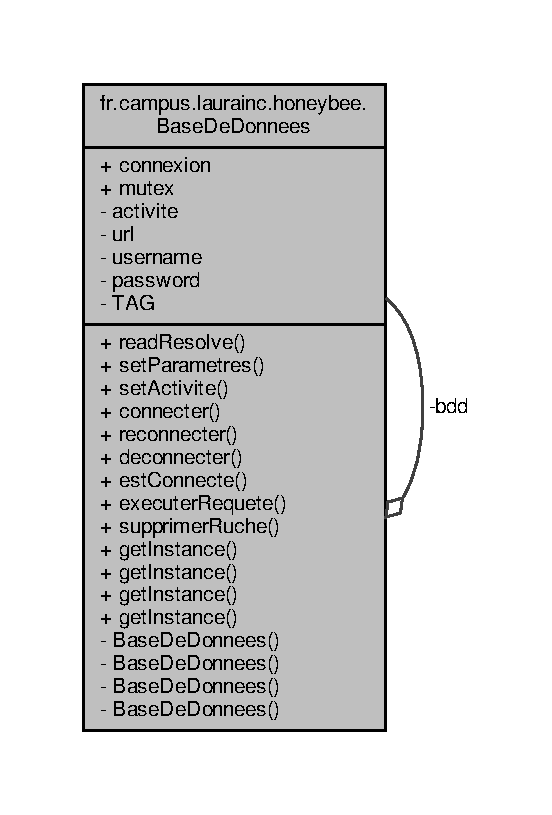
\includegraphics[width=265pt]{classfr_1_1campus_1_1laurainc_1_1honeybee_1_1_base_de_donnees__coll__graph}
\end{center}
\end{figure}
\subsubsection*{Classes}
\begin{DoxyCompactItemize}
\item 
class \hyperlink{classfr_1_1campus_1_1laurainc_1_1honeybee_1_1_base_de_donnees_1_1_connexion_my_sql}{Connexion\+My\+Sql}
\begin{DoxyCompactList}\small\item\em Classe permettant de se connecter à My\+S\+QL en arrière-\/plan. \end{DoxyCompactList}\end{DoxyCompactItemize}
\subsubsection*{Fonctions membres publiques}
\begin{DoxyCompactItemize}
\item 
Object \hyperlink{classfr_1_1campus_1_1laurainc_1_1honeybee_1_1_base_de_donnees_a356a61d32b2d1fdac4e35c04f969fa00}{read\+Resolve} ()
\begin{DoxyCompactList}\small\item\em Retourne l\textquotesingle{}objet dans un flux (cf. Singleton) \end{DoxyCompactList}\item 
void \hyperlink{classfr_1_1campus_1_1laurainc_1_1honeybee_1_1_base_de_donnees_a0960cb9d71647e80e195a580f90cd0d6}{set\+Parametres} (String \hyperlink{classfr_1_1campus_1_1laurainc_1_1honeybee_1_1_base_de_donnees_ad1d04b4da375002e91d8370b9d19918e}{url}, String \hyperlink{classfr_1_1campus_1_1laurainc_1_1honeybee_1_1_base_de_donnees_a7d1662e10f11f740155774b625ed1a87}{username}, String \hyperlink{classfr_1_1campus_1_1laurainc_1_1honeybee_1_1_base_de_donnees_af1bb604a666a7eee9edd93b6cafaf064}{password})
\begin{DoxyCompactList}\small\item\em Modifie les paramètres de connexion à la base de donnees et se reconnecte. \end{DoxyCompactList}\item 
void \hyperlink{classfr_1_1campus_1_1laurainc_1_1honeybee_1_1_base_de_donnees_a4d5b875376c84e702c60bb54cee58c3f}{set\+Activite} (Activity \hyperlink{classfr_1_1campus_1_1laurainc_1_1honeybee_1_1_base_de_donnees_aad4fd29f29916bc4277fa16262d19431}{activite})
\begin{DoxyCompactList}\small\item\em Fixe l\textquotesingle{}activité appelante associée à l\textquotesingle{}instance de Base de données. \end{DoxyCompactList}\item 
boolean \hyperlink{classfr_1_1campus_1_1laurainc_1_1honeybee_1_1_base_de_donnees_a08564ea7dccde161d6eac4b8879401bb}{connecter} ()
\begin{DoxyCompactList}\small\item\em Connexion à la base de données My\+S\+QL si pas déjà connecté \end{DoxyCompactList}\item 
boolean \hyperlink{classfr_1_1campus_1_1laurainc_1_1honeybee_1_1_base_de_donnees_a89357a1cc8a3648400df37a8bfe95958}{reconnecter} ()
\begin{DoxyCompactList}\small\item\em Reconnexion à la base de données My\+S\+QL. \end{DoxyCompactList}\item 
boolean \hyperlink{classfr_1_1campus_1_1laurainc_1_1honeybee_1_1_base_de_donnees_ae022ff0b4923d637f8d392cb908aa252}{deconnecter} ()
\begin{DoxyCompactList}\small\item\em Déconnexion de la base de données My\+S\+QL. \end{DoxyCompactList}\item 
boolean \hyperlink{classfr_1_1campus_1_1laurainc_1_1honeybee_1_1_base_de_donnees_a735f54c2c183a595c9a9a5ba947491f5}{est\+Connecte} ()
\begin{DoxyCompactList}\small\item\em Retourne vrai si on est connecté à la base de données My\+S\+QL. \end{DoxyCompactList}\item 
void \hyperlink{classfr_1_1campus_1_1laurainc_1_1honeybee_1_1_base_de_donnees_a421bffe6f14c01bee64695e7b6a9745d}{executer\+Requete} (final String requete)
\begin{DoxyCompactList}\small\item\em Méthode qui exécute une requête U\+P\+D\+A\+TE, I\+N\+S\+E\+RT ou D\+E\+L\+E\+TE en arrière-\/plan. \end{DoxyCompactList}\item 
void \hyperlink{classfr_1_1campus_1_1laurainc_1_1honeybee_1_1_base_de_donnees_a7b0977566d74684fab184f7a5efce3c8}{supprimer\+Ruche} (final int id\+Ruche)
\end{DoxyCompactItemize}
\subsubsection*{Fonctions membres publiques statiques}
\begin{DoxyCompactItemize}
\item 
static synchronized \hyperlink{classfr_1_1campus_1_1laurainc_1_1honeybee_1_1_base_de_donnees}{Base\+De\+Donnees} \hyperlink{classfr_1_1campus_1_1laurainc_1_1honeybee_1_1_base_de_donnees_a9c2484cfb87f90e46cf878eb7803abb2}{get\+Instance} ()
\begin{DoxyCompactList}\small\item\em Retourne l\textquotesingle{}instance \hyperlink{classfr_1_1campus_1_1laurainc_1_1honeybee_1_1_base_de_donnees}{Base\+De\+Donnees}. \end{DoxyCompactList}\item 
static synchronized \hyperlink{classfr_1_1campus_1_1laurainc_1_1honeybee_1_1_base_de_donnees}{Base\+De\+Donnees} \hyperlink{classfr_1_1campus_1_1laurainc_1_1honeybee_1_1_base_de_donnees_a1946bd458844214e84a5bc1327bbd174}{get\+Instance} (Activity \hyperlink{classfr_1_1campus_1_1laurainc_1_1honeybee_1_1_base_de_donnees_aad4fd29f29916bc4277fa16262d19431}{activite})
\item 
static synchronized \hyperlink{classfr_1_1campus_1_1laurainc_1_1honeybee_1_1_base_de_donnees}{Base\+De\+Donnees} \hyperlink{classfr_1_1campus_1_1laurainc_1_1honeybee_1_1_base_de_donnees_aca2ad0b53f5c21c6a16a7956646c195b}{get\+Instance} (String \hyperlink{classfr_1_1campus_1_1laurainc_1_1honeybee_1_1_base_de_donnees_ad1d04b4da375002e91d8370b9d19918e}{url}, String \hyperlink{classfr_1_1campus_1_1laurainc_1_1honeybee_1_1_base_de_donnees_a7d1662e10f11f740155774b625ed1a87}{username}, String \hyperlink{classfr_1_1campus_1_1laurainc_1_1honeybee_1_1_base_de_donnees_af1bb604a666a7eee9edd93b6cafaf064}{password})
\item 
static synchronized \hyperlink{classfr_1_1campus_1_1laurainc_1_1honeybee_1_1_base_de_donnees}{Base\+De\+Donnees} \hyperlink{classfr_1_1campus_1_1laurainc_1_1honeybee_1_1_base_de_donnees_a8dd37561ed70a74841590d9206248d9b}{get\+Instance} (Activity \hyperlink{classfr_1_1campus_1_1laurainc_1_1honeybee_1_1_base_de_donnees_aad4fd29f29916bc4277fa16262d19431}{activite}, String \hyperlink{classfr_1_1campus_1_1laurainc_1_1honeybee_1_1_base_de_donnees_ad1d04b4da375002e91d8370b9d19918e}{url}, String \hyperlink{classfr_1_1campus_1_1laurainc_1_1honeybee_1_1_base_de_donnees_a7d1662e10f11f740155774b625ed1a87}{username}, String \hyperlink{classfr_1_1campus_1_1laurainc_1_1honeybee_1_1_base_de_donnees_af1bb604a666a7eee9edd93b6cafaf064}{password})
\end{DoxyCompactItemize}
\subsubsection*{Attributs publics statiques}
\begin{DoxyCompactItemize}
\item 
static Connection \hyperlink{classfr_1_1campus_1_1laurainc_1_1honeybee_1_1_base_de_donnees_a358899633f17b8cd00dd2c4cfdd40abe}{connexion} = null
\begin{DoxyCompactList}\small\item\em objet de connexion à My\+S\+QL (null par défaut) \end{DoxyCompactList}\item 
static final Lock \hyperlink{classfr_1_1campus_1_1laurainc_1_1honeybee_1_1_base_de_donnees_a0dd6f285a11459c086adea6080bed282}{mutex} = new Reentrant\+Lock(true)
\begin{DoxyCompactList}\small\item\em mutex pour l\textquotesingle{}exécution concurrente de requêtes \end{DoxyCompactList}\end{DoxyCompactItemize}
\subsubsection*{Fonctions membres privées}
\begin{DoxyCompactItemize}
\item 
\hyperlink{classfr_1_1campus_1_1laurainc_1_1honeybee_1_1_base_de_donnees_ac4d0c514f439b3a19dc35c159955373a}{Base\+De\+Donnees} ()
\begin{DoxyCompactList}\small\item\em Constructeur par défaut de la classe \hyperlink{classfr_1_1campus_1_1laurainc_1_1honeybee_1_1_base_de_donnees}{Base\+De\+Donnees}. \end{DoxyCompactList}\item 
\hyperlink{classfr_1_1campus_1_1laurainc_1_1honeybee_1_1_base_de_donnees_a3023d75b636efcfbb2c6b6ac5c702c42}{Base\+De\+Donnees} (Activity \hyperlink{classfr_1_1campus_1_1laurainc_1_1honeybee_1_1_base_de_donnees_aad4fd29f29916bc4277fa16262d19431}{activite})
\item 
\hyperlink{classfr_1_1campus_1_1laurainc_1_1honeybee_1_1_base_de_donnees_a2f6274017a47cc8f331c582f9a7ad6d1}{Base\+De\+Donnees} (String \hyperlink{classfr_1_1campus_1_1laurainc_1_1honeybee_1_1_base_de_donnees_ad1d04b4da375002e91d8370b9d19918e}{url}, String \hyperlink{classfr_1_1campus_1_1laurainc_1_1honeybee_1_1_base_de_donnees_a7d1662e10f11f740155774b625ed1a87}{username}, String \hyperlink{classfr_1_1campus_1_1laurainc_1_1honeybee_1_1_base_de_donnees_af1bb604a666a7eee9edd93b6cafaf064}{password})
\item 
\hyperlink{classfr_1_1campus_1_1laurainc_1_1honeybee_1_1_base_de_donnees_ab3a19c26fc4ddbddc1d9166e88bb4db7}{Base\+De\+Donnees} (Activity \hyperlink{classfr_1_1campus_1_1laurainc_1_1honeybee_1_1_base_de_donnees_aad4fd29f29916bc4277fa16262d19431}{activite}, String \hyperlink{classfr_1_1campus_1_1laurainc_1_1honeybee_1_1_base_de_donnees_ad1d04b4da375002e91d8370b9d19918e}{url}, String \hyperlink{classfr_1_1campus_1_1laurainc_1_1honeybee_1_1_base_de_donnees_a7d1662e10f11f740155774b625ed1a87}{username}, String \hyperlink{classfr_1_1campus_1_1laurainc_1_1honeybee_1_1_base_de_donnees_af1bb604a666a7eee9edd93b6cafaf064}{password})
\end{DoxyCompactItemize}
\subsubsection*{Attributs privés}
\begin{DoxyCompactItemize}
\item 
Activity \hyperlink{classfr_1_1campus_1_1laurainc_1_1honeybee_1_1_base_de_donnees_aad4fd29f29916bc4277fa16262d19431}{activite} = null
\begin{DoxyCompactList}\small\item\em objet sur l\textquotesingle{}activite ayant créé l\textquotesingle{}objet \hyperlink{classfr_1_1campus_1_1laurainc_1_1honeybee_1_1_base_de_donnees}{Base\+De\+Donnees} (si besoin pour UI) \end{DoxyCompactList}\item 
String \hyperlink{classfr_1_1campus_1_1laurainc_1_1honeybee_1_1_base_de_donnees_ad1d04b4da375002e91d8370b9d19918e}{url}
\begin{DoxyCompactList}\small\item\em l\textquotesingle{}U\+RL pointant sur la base de données d\textquotesingle{}un serveur My\+S\+QL \end{DoxyCompactList}\item 
String \hyperlink{classfr_1_1campus_1_1laurainc_1_1honeybee_1_1_base_de_donnees_a7d1662e10f11f740155774b625ed1a87}{username}
\begin{DoxyCompactList}\small\item\em le nom du compte utilisateur (root par défaut) \end{DoxyCompactList}\item 
String \hyperlink{classfr_1_1campus_1_1laurainc_1_1honeybee_1_1_base_de_donnees_af1bb604a666a7eee9edd93b6cafaf064}{password}
\begin{DoxyCompactList}\small\item\em le mot de passe du compte utilisateur (password par défaut) \end{DoxyCompactList}\end{DoxyCompactItemize}
\subsubsection*{Attributs privés statiques}
\begin{DoxyCompactItemize}
\item 
static final String \hyperlink{classfr_1_1campus_1_1laurainc_1_1honeybee_1_1_base_de_donnees_ae800d867b3e423dd139e982736ab5587}{T\+AG} = \char`\"{}Base\+De\+Donnees\char`\"{}
\begin{DoxyCompactList}\small\item\em le T\+AG de la classe pour les logs \end{DoxyCompactList}\item 
static \hyperlink{classfr_1_1campus_1_1laurainc_1_1honeybee_1_1_base_de_donnees}{Base\+De\+Donnees} \hyperlink{classfr_1_1campus_1_1laurainc_1_1honeybee_1_1_base_de_donnees_a6afcd3f4c69f15afa0c675a848bf97a7}{bdd} = null
\begin{DoxyCompactList}\small\item\em l\textquotesingle{}instance unique de \hyperlink{classfr_1_1campus_1_1laurainc_1_1honeybee_1_1_base_de_donnees}{Base\+De\+Donnees} (Singleton) \end{DoxyCompactList}\end{DoxyCompactItemize}


\subsubsection{Description détaillée}
\begin{DoxyAuthor}{Auteur}
Thierry Vaira 
\end{DoxyAuthor}


\subsubsection{Documentation des constructeurs et destructeur}
\mbox{\Hypertarget{classfr_1_1campus_1_1laurainc_1_1honeybee_1_1_base_de_donnees_ac4d0c514f439b3a19dc35c159955373a}\label{classfr_1_1campus_1_1laurainc_1_1honeybee_1_1_base_de_donnees_ac4d0c514f439b3a19dc35c159955373a}} 
\index{fr\+::campus\+::laurainc\+::honeybee\+::\+Base\+De\+Donnees@{fr\+::campus\+::laurainc\+::honeybee\+::\+Base\+De\+Donnees}!Base\+De\+Donnees@{Base\+De\+Donnees}}
\index{Base\+De\+Donnees@{Base\+De\+Donnees}!fr\+::campus\+::laurainc\+::honeybee\+::\+Base\+De\+Donnees@{fr\+::campus\+::laurainc\+::honeybee\+::\+Base\+De\+Donnees}}
\paragraph{\texorpdfstring{Base\+De\+Donnees()}{BaseDeDonnees()}\hspace{0.1cm}{\footnotesize\ttfamily [1/4]}}
{\footnotesize\ttfamily Base\+De\+Donnees.\+Base\+De\+Donnees (\begin{DoxyParamCaption}{ }\end{DoxyParamCaption})\hspace{0.3cm}{\ttfamily [private]}}

Constructeur de la classe \hyperlink{classfr_1_1campus_1_1laurainc_1_1honeybee_1_1_base_de_donnees}{Base\+De\+Donnees}.


\begin{DoxyParams}{Paramètres}
{\em activite} & Activity l\textquotesingle{}activité appelante\\
\hline
{\em url} & String l\textquotesingle{}U\+RL pointant sur la base de données d\textquotesingle{}un serveur My\+S\+QL \\
\hline
{\em username} & String le nom d\textquotesingle{}utilisateur \\
\hline
{\em password} & String le mot de passe de l\textquotesingle{}utilisateur\\
\hline
{\em activite} & Activity l\textquotesingle{}activité appelante \\
\hline
{\em url} & String l\textquotesingle{}U\+RL pointant sur la base de données d\textquotesingle{}un serveur My\+S\+QL \\
\hline
{\em username} & String le nom d\textquotesingle{}utilisateur \\
\hline
{\em password} & String le mot de passe de l\textquotesingle{}utilisateur \\
\hline
\end{DoxyParams}


Référencé par \hyperlink{classfr_1_1campus_1_1laurainc_1_1honeybee_1_1_base_de_donnees_a9c2484cfb87f90e46cf878eb7803abb2}{fr.\+campus.\+laurainc.\+honeybee.\+Base\+De\+Donnees.\+get\+Instance()}.


\begin{DoxyCode}
00107     \{
00108     \}
\end{DoxyCode}
\mbox{\Hypertarget{classfr_1_1campus_1_1laurainc_1_1honeybee_1_1_base_de_donnees_a3023d75b636efcfbb2c6b6ac5c702c42}\label{classfr_1_1campus_1_1laurainc_1_1honeybee_1_1_base_de_donnees_a3023d75b636efcfbb2c6b6ac5c702c42}} 
\index{fr\+::campus\+::laurainc\+::honeybee\+::\+Base\+De\+Donnees@{fr\+::campus\+::laurainc\+::honeybee\+::\+Base\+De\+Donnees}!Base\+De\+Donnees@{Base\+De\+Donnees}}
\index{Base\+De\+Donnees@{Base\+De\+Donnees}!fr\+::campus\+::laurainc\+::honeybee\+::\+Base\+De\+Donnees@{fr\+::campus\+::laurainc\+::honeybee\+::\+Base\+De\+Donnees}}
\paragraph{\texorpdfstring{Base\+De\+Donnees()}{BaseDeDonnees()}\hspace{0.1cm}{\footnotesize\ttfamily [2/4]}}
{\footnotesize\ttfamily fr.\+campus.\+laurainc.\+honeybee.\+Base\+De\+Donnees.\+Base\+De\+Donnees (\begin{DoxyParamCaption}\item[{Activity}]{activite }\end{DoxyParamCaption})\hspace{0.3cm}{\ttfamily [private]}}



Références \hyperlink{classfr_1_1campus_1_1laurainc_1_1honeybee_1_1_base_de_donnees_aad4fd29f29916bc4277fa16262d19431}{fr.\+campus.\+laurainc.\+honeybee.\+Base\+De\+Donnees.\+activite}.


\begin{DoxyCode}
00116     \{
00117         this.\hyperlink{classfr_1_1campus_1_1laurainc_1_1honeybee_1_1_base_de_donnees_aad4fd29f29916bc4277fa16262d19431}{activite} = \hyperlink{classfr_1_1campus_1_1laurainc_1_1honeybee_1_1_base_de_donnees_aad4fd29f29916bc4277fa16262d19431}{activite};
00118     \}
\end{DoxyCode}
\mbox{\Hypertarget{classfr_1_1campus_1_1laurainc_1_1honeybee_1_1_base_de_donnees_a2f6274017a47cc8f331c582f9a7ad6d1}\label{classfr_1_1campus_1_1laurainc_1_1honeybee_1_1_base_de_donnees_a2f6274017a47cc8f331c582f9a7ad6d1}} 
\index{fr\+::campus\+::laurainc\+::honeybee\+::\+Base\+De\+Donnees@{fr\+::campus\+::laurainc\+::honeybee\+::\+Base\+De\+Donnees}!Base\+De\+Donnees@{Base\+De\+Donnees}}
\index{Base\+De\+Donnees@{Base\+De\+Donnees}!fr\+::campus\+::laurainc\+::honeybee\+::\+Base\+De\+Donnees@{fr\+::campus\+::laurainc\+::honeybee\+::\+Base\+De\+Donnees}}
\paragraph{\texorpdfstring{Base\+De\+Donnees()}{BaseDeDonnees()}\hspace{0.1cm}{\footnotesize\ttfamily [3/4]}}
{\footnotesize\ttfamily fr.\+campus.\+laurainc.\+honeybee.\+Base\+De\+Donnees.\+Base\+De\+Donnees (\begin{DoxyParamCaption}\item[{String}]{url,  }\item[{String}]{username,  }\item[{String}]{password }\end{DoxyParamCaption})\hspace{0.3cm}{\ttfamily [private]}}



Références \hyperlink{classfr_1_1campus_1_1laurainc_1_1honeybee_1_1_base_de_donnees_a08564ea7dccde161d6eac4b8879401bb}{fr.\+campus.\+laurainc.\+honeybee.\+Base\+De\+Donnees.\+connecter()}, \hyperlink{classfr_1_1campus_1_1laurainc_1_1honeybee_1_1_base_de_donnees_af1bb604a666a7eee9edd93b6cafaf064}{fr.\+campus.\+laurainc.\+honeybee.\+Base\+De\+Donnees.\+password}, \hyperlink{classfr_1_1campus_1_1laurainc_1_1honeybee_1_1_base_de_donnees_ad1d04b4da375002e91d8370b9d19918e}{fr.\+campus.\+laurainc.\+honeybee.\+Base\+De\+Donnees.\+url}, et \hyperlink{classfr_1_1campus_1_1laurainc_1_1honeybee_1_1_base_de_donnees_a7d1662e10f11f740155774b625ed1a87}{fr.\+campus.\+laurainc.\+honeybee.\+Base\+De\+Donnees.\+username}.


\begin{DoxyCode}
00128     \{
00129         Log.v(\hyperlink{classfr_1_1campus_1_1laurainc_1_1honeybee_1_1_base_de_donnees_ae800d867b3e423dd139e982736ab5587}{TAG}, \textcolor{stringliteral}{"url="} + \hyperlink{classfr_1_1campus_1_1laurainc_1_1honeybee_1_1_base_de_donnees_ad1d04b4da375002e91d8370b9d19918e}{url});
00130         Log.v(\hyperlink{classfr_1_1campus_1_1laurainc_1_1honeybee_1_1_base_de_donnees_ae800d867b3e423dd139e982736ab5587}{TAG}, \textcolor{stringliteral}{"username="} + \hyperlink{classfr_1_1campus_1_1laurainc_1_1honeybee_1_1_base_de_donnees_a7d1662e10f11f740155774b625ed1a87}{username});
00131         Log.v(\hyperlink{classfr_1_1campus_1_1laurainc_1_1honeybee_1_1_base_de_donnees_ae800d867b3e423dd139e982736ab5587}{TAG}, \textcolor{stringliteral}{"password="} + \hyperlink{classfr_1_1campus_1_1laurainc_1_1honeybee_1_1_base_de_donnees_af1bb604a666a7eee9edd93b6cafaf064}{password});
00132         this.\hyperlink{classfr_1_1campus_1_1laurainc_1_1honeybee_1_1_base_de_donnees_ad1d04b4da375002e91d8370b9d19918e}{url} = \hyperlink{classfr_1_1campus_1_1laurainc_1_1honeybee_1_1_base_de_donnees_ad1d04b4da375002e91d8370b9d19918e}{url};
00133         this.\hyperlink{classfr_1_1campus_1_1laurainc_1_1honeybee_1_1_base_de_donnees_a7d1662e10f11f740155774b625ed1a87}{username} = \hyperlink{classfr_1_1campus_1_1laurainc_1_1honeybee_1_1_base_de_donnees_a7d1662e10f11f740155774b625ed1a87}{username};
00134         this.\hyperlink{classfr_1_1campus_1_1laurainc_1_1honeybee_1_1_base_de_donnees_af1bb604a666a7eee9edd93b6cafaf064}{password} = \hyperlink{classfr_1_1campus_1_1laurainc_1_1honeybee_1_1_base_de_donnees_af1bb604a666a7eee9edd93b6cafaf064}{password};
00135         \textcolor{comment}{// on peut se connecter}
00136         \hyperlink{classfr_1_1campus_1_1laurainc_1_1honeybee_1_1_base_de_donnees_a08564ea7dccde161d6eac4b8879401bb}{connecter}();
00137     \}
\end{DoxyCode}
\mbox{\Hypertarget{classfr_1_1campus_1_1laurainc_1_1honeybee_1_1_base_de_donnees_ab3a19c26fc4ddbddc1d9166e88bb4db7}\label{classfr_1_1campus_1_1laurainc_1_1honeybee_1_1_base_de_donnees_ab3a19c26fc4ddbddc1d9166e88bb4db7}} 
\index{fr\+::campus\+::laurainc\+::honeybee\+::\+Base\+De\+Donnees@{fr\+::campus\+::laurainc\+::honeybee\+::\+Base\+De\+Donnees}!Base\+De\+Donnees@{Base\+De\+Donnees}}
\index{Base\+De\+Donnees@{Base\+De\+Donnees}!fr\+::campus\+::laurainc\+::honeybee\+::\+Base\+De\+Donnees@{fr\+::campus\+::laurainc\+::honeybee\+::\+Base\+De\+Donnees}}
\paragraph{\texorpdfstring{Base\+De\+Donnees()}{BaseDeDonnees()}\hspace{0.1cm}{\footnotesize\ttfamily [4/4]}}
{\footnotesize\ttfamily fr.\+campus.\+laurainc.\+honeybee.\+Base\+De\+Donnees.\+Base\+De\+Donnees (\begin{DoxyParamCaption}\item[{Activity}]{activite,  }\item[{String}]{url,  }\item[{String}]{username,  }\item[{String}]{password }\end{DoxyParamCaption})\hspace{0.3cm}{\ttfamily [private]}}



Références \hyperlink{classfr_1_1campus_1_1laurainc_1_1honeybee_1_1_base_de_donnees_aad4fd29f29916bc4277fa16262d19431}{fr.\+campus.\+laurainc.\+honeybee.\+Base\+De\+Donnees.\+activite}, \hyperlink{classfr_1_1campus_1_1laurainc_1_1honeybee_1_1_base_de_donnees_a08564ea7dccde161d6eac4b8879401bb}{fr.\+campus.\+laurainc.\+honeybee.\+Base\+De\+Donnees.\+connecter()}, \hyperlink{classfr_1_1campus_1_1laurainc_1_1honeybee_1_1_base_de_donnees_af1bb604a666a7eee9edd93b6cafaf064}{fr.\+campus.\+laurainc.\+honeybee.\+Base\+De\+Donnees.\+password}, \hyperlink{classfr_1_1campus_1_1laurainc_1_1honeybee_1_1_base_de_donnees_ad1d04b4da375002e91d8370b9d19918e}{fr.\+campus.\+laurainc.\+honeybee.\+Base\+De\+Donnees.\+url}, et \hyperlink{classfr_1_1campus_1_1laurainc_1_1honeybee_1_1_base_de_donnees_a7d1662e10f11f740155774b625ed1a87}{fr.\+campus.\+laurainc.\+honeybee.\+Base\+De\+Donnees.\+username}.


\begin{DoxyCode}
00148     \{
00149         Log.v(\hyperlink{classfr_1_1campus_1_1laurainc_1_1honeybee_1_1_base_de_donnees_ae800d867b3e423dd139e982736ab5587}{TAG}, \textcolor{stringliteral}{"url="} + \hyperlink{classfr_1_1campus_1_1laurainc_1_1honeybee_1_1_base_de_donnees_ad1d04b4da375002e91d8370b9d19918e}{url});
00150         Log.v(\hyperlink{classfr_1_1campus_1_1laurainc_1_1honeybee_1_1_base_de_donnees_ae800d867b3e423dd139e982736ab5587}{TAG}, \textcolor{stringliteral}{"username="} + \hyperlink{classfr_1_1campus_1_1laurainc_1_1honeybee_1_1_base_de_donnees_a7d1662e10f11f740155774b625ed1a87}{username});
00151         Log.v(\hyperlink{classfr_1_1campus_1_1laurainc_1_1honeybee_1_1_base_de_donnees_ae800d867b3e423dd139e982736ab5587}{TAG}, \textcolor{stringliteral}{"password="} + \hyperlink{classfr_1_1campus_1_1laurainc_1_1honeybee_1_1_base_de_donnees_af1bb604a666a7eee9edd93b6cafaf064}{password});
00152         this.\hyperlink{classfr_1_1campus_1_1laurainc_1_1honeybee_1_1_base_de_donnees_aad4fd29f29916bc4277fa16262d19431}{activite} = \hyperlink{classfr_1_1campus_1_1laurainc_1_1honeybee_1_1_base_de_donnees_aad4fd29f29916bc4277fa16262d19431}{activite};
00153         this.\hyperlink{classfr_1_1campus_1_1laurainc_1_1honeybee_1_1_base_de_donnees_ad1d04b4da375002e91d8370b9d19918e}{url} = \hyperlink{classfr_1_1campus_1_1laurainc_1_1honeybee_1_1_base_de_donnees_ad1d04b4da375002e91d8370b9d19918e}{url};
00154         this.\hyperlink{classfr_1_1campus_1_1laurainc_1_1honeybee_1_1_base_de_donnees_a7d1662e10f11f740155774b625ed1a87}{username} = \hyperlink{classfr_1_1campus_1_1laurainc_1_1honeybee_1_1_base_de_donnees_a7d1662e10f11f740155774b625ed1a87}{username};
00155         this.\hyperlink{classfr_1_1campus_1_1laurainc_1_1honeybee_1_1_base_de_donnees_af1bb604a666a7eee9edd93b6cafaf064}{password} = \hyperlink{classfr_1_1campus_1_1laurainc_1_1honeybee_1_1_base_de_donnees_af1bb604a666a7eee9edd93b6cafaf064}{password};
00156         \textcolor{comment}{// on peut se connecter}
00157         \hyperlink{classfr_1_1campus_1_1laurainc_1_1honeybee_1_1_base_de_donnees_a08564ea7dccde161d6eac4b8879401bb}{connecter}();
00158     \}
\end{DoxyCode}


\subsubsection{Documentation des fonctions membres}
\mbox{\Hypertarget{classfr_1_1campus_1_1laurainc_1_1honeybee_1_1_base_de_donnees_a08564ea7dccde161d6eac4b8879401bb}\label{classfr_1_1campus_1_1laurainc_1_1honeybee_1_1_base_de_donnees_a08564ea7dccde161d6eac4b8879401bb}} 
\index{fr\+::campus\+::laurainc\+::honeybee\+::\+Base\+De\+Donnees@{fr\+::campus\+::laurainc\+::honeybee\+::\+Base\+De\+Donnees}!connecter@{connecter}}
\index{connecter@{connecter}!fr\+::campus\+::laurainc\+::honeybee\+::\+Base\+De\+Donnees@{fr\+::campus\+::laurainc\+::honeybee\+::\+Base\+De\+Donnees}}
\paragraph{\texorpdfstring{connecter()}{connecter()}}
{\footnotesize\ttfamily Base\+De\+Donnees.\+connecter (\begin{DoxyParamCaption}{ }\end{DoxyParamCaption})}

\begin{DoxyReturn}{Renvoie}
boolean vrai si la connexion a réussi sinon faux 
\end{DoxyReturn}


Références \hyperlink{classfr_1_1campus_1_1laurainc_1_1honeybee_1_1_honey_bee_abfb4f6cc1c8bb793c37ccb8408abc51c}{fr.\+campus.\+laurainc.\+honeybee.\+Honey\+Bee.\+B\+DD}, et \hyperlink{classfr_1_1campus_1_1laurainc_1_1honeybee_1_1_base_de_donnees_a735f54c2c183a595c9a9a5ba947491f5}{fr.\+campus.\+laurainc.\+honeybee.\+Base\+De\+Donnees.\+est\+Connecte()}.



Référencé par \hyperlink{classfr_1_1campus_1_1laurainc_1_1honeybee_1_1_base_de_donnees_a2f6274017a47cc8f331c582f9a7ad6d1}{fr.\+campus.\+laurainc.\+honeybee.\+Base\+De\+Donnees.\+Base\+De\+Donnees()}, \hyperlink{classfr_1_1campus_1_1laurainc_1_1honeybee_1_1_main_activity_aba2e570bbba3bf1be8487068d9c6c2da}{fr.\+campus.\+laurainc.\+honeybee.\+Main\+Activity.\+on\+Create()}, \hyperlink{classfr_1_1campus_1_1laurainc_1_1honeybee_1_1_nouvelle_ruche_activity_ae97fec78fb0a2e1cc4610182bc71ea0d}{fr.\+campus.\+laurainc.\+honeybee.\+Nouvelle\+Ruche\+Activity.\+on\+Create()}, \hyperlink{classfr_1_1campus_1_1laurainc_1_1honeybee_1_1_base_de_donnees_a89357a1cc8a3648400df37a8bfe95958}{fr.\+campus.\+laurainc.\+honeybee.\+Base\+De\+Donnees.\+reconnecter()}, et \hyperlink{classfr_1_1campus_1_1laurainc_1_1honeybee_1_1_ruche_a56ec53516e4f94b4f5e42f083fa345db}{fr.\+campus.\+laurainc.\+honeybee.\+Ruche.\+Ruche()}.


\begin{DoxyCode}
00192     \{
00193         \textcolor{keywordflow}{if}(!HoneyBee.BDD)
00194             \textcolor{keywordflow}{return} \textcolor{keyword}{false};
00195 
00196         \textcolor{keywordflow}{try}
00197         \{
00198             \textcolor{keywordflow}{if} (!\hyperlink{classfr_1_1campus_1_1laurainc_1_1honeybee_1_1_base_de_donnees_a735f54c2c183a595c9a9a5ba947491f5}{estConnecte}())
00199             \{
00200                 ConnexionMySql connexionMySql = \textcolor{keyword}{new} ConnexionMySql();
00201                 connexionMySql.execute();
00202                 Log.d(\hyperlink{classfr_1_1campus_1_1laurainc_1_1honeybee_1_1_base_de_donnees_ae800d867b3e423dd139e982736ab5587}{TAG}, \textcolor{stringliteral}{"connecter -> retour : "} + connexionMySql.get());
00203                 \textcolor{keywordflow}{return} connexionMySql.get();
00204             \}
00205             \textcolor{keywordflow}{return} \textcolor{keyword}{true};
00206         \}
00207         \textcolor{keywordflow}{catch} (InterruptedException e)
00208         \{
00209             e.printStackTrace();
00210             Log.e(\hyperlink{classfr_1_1campus_1_1laurainc_1_1honeybee_1_1_base_de_donnees_ae800d867b3e423dd139e982736ab5587}{TAG}, \textcolor{stringliteral}{"connecter -> InterruptedException : "} + e.toString());
00211             \textcolor{keywordflow}{return} \textcolor{keyword}{false};
00212         \}
00213         \textcolor{keywordflow}{catch} (ExecutionException e)
00214         \{
00215             e.printStackTrace();
00216             Log.e(\hyperlink{classfr_1_1campus_1_1laurainc_1_1honeybee_1_1_base_de_donnees_ae800d867b3e423dd139e982736ab5587}{TAG}, \textcolor{stringliteral}{"connecter -> ExecutionException : "} + e.toString());
00217             \textcolor{keywordflow}{return} \textcolor{keyword}{false};
00218         \}
00219     \}
\end{DoxyCode}
\mbox{\Hypertarget{classfr_1_1campus_1_1laurainc_1_1honeybee_1_1_base_de_donnees_ae022ff0b4923d637f8d392cb908aa252}\label{classfr_1_1campus_1_1laurainc_1_1honeybee_1_1_base_de_donnees_ae022ff0b4923d637f8d392cb908aa252}} 
\index{fr\+::campus\+::laurainc\+::honeybee\+::\+Base\+De\+Donnees@{fr\+::campus\+::laurainc\+::honeybee\+::\+Base\+De\+Donnees}!deconnecter@{deconnecter}}
\index{deconnecter@{deconnecter}!fr\+::campus\+::laurainc\+::honeybee\+::\+Base\+De\+Donnees@{fr\+::campus\+::laurainc\+::honeybee\+::\+Base\+De\+Donnees}}
\paragraph{\texorpdfstring{deconnecter()}{deconnecter()}}
{\footnotesize\ttfamily Base\+De\+Donnees.\+deconnecter (\begin{DoxyParamCaption}{ }\end{DoxyParamCaption})}

\begin{DoxyReturn}{Renvoie}
boolean vrai si la déconnexion a réussi sinon faux 
\end{DoxyReturn}


Références \hyperlink{classfr_1_1campus_1_1laurainc_1_1honeybee_1_1_honey_bee_abfb4f6cc1c8bb793c37ccb8408abc51c}{fr.\+campus.\+laurainc.\+honeybee.\+Honey\+Bee.\+B\+DD}.



Référencé par \hyperlink{classfr_1_1campus_1_1laurainc_1_1honeybee_1_1_base_de_donnees_a89357a1cc8a3648400df37a8bfe95958}{fr.\+campus.\+laurainc.\+honeybee.\+Base\+De\+Donnees.\+reconnecter()}.


\begin{DoxyCode}
00240     \{
00241         \textcolor{keywordflow}{if} (!HoneyBee.BDD)
00242             \textcolor{keywordflow}{return} \textcolor{keyword}{false};
00243 
00244         \textcolor{keywordflow}{try}
00245         \{
00246             \textcolor{keywordflow}{if} (\hyperlink{classfr_1_1campus_1_1laurainc_1_1honeybee_1_1_base_de_donnees_a358899633f17b8cd00dd2c4cfdd40abe}{connexion} != null)
00247             \{
00248                 \hyperlink{classfr_1_1campus_1_1laurainc_1_1honeybee_1_1_base_de_donnees_a358899633f17b8cd00dd2c4cfdd40abe}{connexion}.close();
00249                 Log.d(\hyperlink{classfr_1_1campus_1_1laurainc_1_1honeybee_1_1_base_de_donnees_ae800d867b3e423dd139e982736ab5587}{TAG}, \textcolor{stringliteral}{"deconnecter -> retour : "} + \hyperlink{classfr_1_1campus_1_1laurainc_1_1honeybee_1_1_base_de_donnees_a358899633f17b8cd00dd2c4cfdd40abe}{connexion}.isClosed());
00250                 \textcolor{keywordflow}{return} \hyperlink{classfr_1_1campus_1_1laurainc_1_1honeybee_1_1_base_de_donnees_a358899633f17b8cd00dd2c4cfdd40abe}{connexion}.isClosed();
00251             \}
00252             \textcolor{keywordflow}{return} \textcolor{keyword}{true};
00253         \}
00254         \textcolor{keywordflow}{catch} (SQLException e)
00255         \{
00256             e.printStackTrace();
00257             Log.e(\hyperlink{classfr_1_1campus_1_1laurainc_1_1honeybee_1_1_base_de_donnees_ae800d867b3e423dd139e982736ab5587}{TAG}, \textcolor{stringliteral}{"deconnecter -> ExecutionException : "} + e.toString());
00258             \textcolor{keywordflow}{return} \textcolor{keyword}{false};
00259         \}
00260     \}
\end{DoxyCode}
\mbox{\Hypertarget{classfr_1_1campus_1_1laurainc_1_1honeybee_1_1_base_de_donnees_a735f54c2c183a595c9a9a5ba947491f5}\label{classfr_1_1campus_1_1laurainc_1_1honeybee_1_1_base_de_donnees_a735f54c2c183a595c9a9a5ba947491f5}} 
\index{fr\+::campus\+::laurainc\+::honeybee\+::\+Base\+De\+Donnees@{fr\+::campus\+::laurainc\+::honeybee\+::\+Base\+De\+Donnees}!est\+Connecte@{est\+Connecte}}
\index{est\+Connecte@{est\+Connecte}!fr\+::campus\+::laurainc\+::honeybee\+::\+Base\+De\+Donnees@{fr\+::campus\+::laurainc\+::honeybee\+::\+Base\+De\+Donnees}}
\paragraph{\texorpdfstring{est\+Connecte()}{estConnecte()}}
{\footnotesize\ttfamily Base\+De\+Donnees.\+est\+Connecte (\begin{DoxyParamCaption}{ }\end{DoxyParamCaption})}

\begin{DoxyReturn}{Renvoie}
boolean vrai si on est connecté à la base de données My\+S\+QL sinon faux 
\end{DoxyReturn}


Références \hyperlink{classfr_1_1campus_1_1laurainc_1_1honeybee_1_1_honey_bee_abfb4f6cc1c8bb793c37ccb8408abc51c}{fr.\+campus.\+laurainc.\+honeybee.\+Honey\+Bee.\+B\+DD}.



Référencé par \hyperlink{classfr_1_1campus_1_1laurainc_1_1honeybee_1_1_base_de_donnees_a08564ea7dccde161d6eac4b8879401bb}{fr.\+campus.\+laurainc.\+honeybee.\+Base\+De\+Donnees.\+connecter()}, \hyperlink{classfr_1_1campus_1_1laurainc_1_1honeybee_1_1_base_de_donnees_1_1_connexion_my_sql_a752c9f0f9a0879fceeeabd48c5fcb058}{fr.\+campus.\+laurainc.\+honeybee.\+Base\+De\+Donnees.\+Connexion\+My\+Sql.\+do\+In\+Background()}, \hyperlink{classfr_1_1campus_1_1laurainc_1_1honeybee_1_1_base_de_donnees_a421bffe6f14c01bee64695e7b6a9745d}{fr.\+campus.\+laurainc.\+honeybee.\+Base\+De\+Donnees.\+executer\+Requete()}, \hyperlink{classfr_1_1campus_1_1laurainc_1_1honeybee_1_1_ruche_a7a99d3c585f2c507eb2c6c265a5bb1fe}{fr.\+campus.\+laurainc.\+honeybee.\+Ruche.\+recuperer()}, \hyperlink{classfr_1_1campus_1_1laurainc_1_1honeybee_1_1_ruche_ade5d681bd0a29d84e0d069169b10a38b}{fr.\+campus.\+laurainc.\+honeybee.\+Ruche.\+recuperer\+Choix\+Ch\+App\+I\+D()}, \hyperlink{classfr_1_1campus_1_1laurainc_1_1honeybee_1_1_ruche_ace10a52a470257f2b8f161fc3c7b9f15}{fr.\+campus.\+laurainc.\+honeybee.\+Ruche.\+recuperer\+Historique\+Alertes()}, \hyperlink{classfr_1_1campus_1_1laurainc_1_1honeybee_1_1_ruche_a1113f3b4a527a801fdf50350667fd212}{fr.\+campus.\+laurainc.\+honeybee.\+Ruche.\+recuperer\+Id\+T\+T\+N()}, \hyperlink{classfr_1_1campus_1_1laurainc_1_1honeybee_1_1_ruche_aba0591cda391b907da41a0afeba4d59d}{fr.\+campus.\+laurainc.\+honeybee.\+Ruche.\+recuperer\+Liste\+Ruches()}, \hyperlink{classfr_1_1campus_1_1laurainc_1_1honeybee_1_1_ruche_a84de3c3af21b1cbeae2075e480acaabc}{fr.\+campus.\+laurainc.\+honeybee.\+Ruche.\+recuperer\+Mesures\+Journalieres\+Ruche()}, \hyperlink{classfr_1_1campus_1_1laurainc_1_1honeybee_1_1_ruche_a94f815b44f0d5d8682833d6b6e783713}{fr.\+campus.\+laurainc.\+honeybee.\+Ruche.\+recuperer\+Moyennes()}, et \hyperlink{classfr_1_1campus_1_1laurainc_1_1honeybee_1_1_base_de_donnees_a7b0977566d74684fab184f7a5efce3c8}{fr.\+campus.\+laurainc.\+honeybee.\+Base\+De\+Donnees.\+supprimer\+Ruche()}.


\begin{DoxyCode}
00268     \{
00269         \textcolor{keywordflow}{if}(!HoneyBee.BDD)
00270             \textcolor{keywordflow}{return} \textcolor{keyword}{false};
00271 
00272         \textcolor{keywordflow}{try}
00273         \{
00274             \textcolor{keywordflow}{if}(\hyperlink{classfr_1_1campus_1_1laurainc_1_1honeybee_1_1_base_de_donnees_a358899633f17b8cd00dd2c4cfdd40abe}{connexion} != null)
00275                 \textcolor{keywordflow}{return} !\hyperlink{classfr_1_1campus_1_1laurainc_1_1honeybee_1_1_base_de_donnees_a358899633f17b8cd00dd2c4cfdd40abe}{connexion}.isClosed();
00276             \textcolor{keywordflow}{else}
00277                 \textcolor{keywordflow}{return} \textcolor{keyword}{false};
00278         \}
00279         \textcolor{keywordflow}{catch} (SQLException e)
00280         \{
00281             e.printStackTrace();
00282             \textcolor{keywordflow}{return} \textcolor{keyword}{false};
00283         \}
00284     \}
\end{DoxyCode}
\mbox{\Hypertarget{classfr_1_1campus_1_1laurainc_1_1honeybee_1_1_base_de_donnees_a421bffe6f14c01bee64695e7b6a9745d}\label{classfr_1_1campus_1_1laurainc_1_1honeybee_1_1_base_de_donnees_a421bffe6f14c01bee64695e7b6a9745d}} 
\index{fr\+::campus\+::laurainc\+::honeybee\+::\+Base\+De\+Donnees@{fr\+::campus\+::laurainc\+::honeybee\+::\+Base\+De\+Donnees}!executer\+Requete@{executer\+Requete}}
\index{executer\+Requete@{executer\+Requete}!fr\+::campus\+::laurainc\+::honeybee\+::\+Base\+De\+Donnees@{fr\+::campus\+::laurainc\+::honeybee\+::\+Base\+De\+Donnees}}
\paragraph{\texorpdfstring{executer\+Requete()}{executerRequete()}}
{\footnotesize\ttfamily Base\+De\+Donnees.\+executer\+Requete (\begin{DoxyParamCaption}\item[{final String}]{requete }\end{DoxyParamCaption})}



Références \hyperlink{classfr_1_1campus_1_1laurainc_1_1honeybee_1_1_honey_bee_abfb4f6cc1c8bb793c37ccb8408abc51c}{fr.\+campus.\+laurainc.\+honeybee.\+Honey\+Bee.\+B\+DD}, et \hyperlink{classfr_1_1campus_1_1laurainc_1_1honeybee_1_1_base_de_donnees_a735f54c2c183a595c9a9a5ba947491f5}{fr.\+campus.\+laurainc.\+honeybee.\+Base\+De\+Donnees.\+est\+Connecte()}.



Référencé par \hyperlink{classfr_1_1campus_1_1laurainc_1_1honeybee_1_1_nouvelle_ruche_activity_ae97fec78fb0a2e1cc4610182bc71ea0d}{fr.\+campus.\+laurainc.\+honeybee.\+Nouvelle\+Ruche\+Activity.\+on\+Create()}.


\begin{DoxyCode}
00390     \{
00391         \textcolor{keywordflow}{if}(!HoneyBee.BDD)
00392             \textcolor{keywordflow}{return};
00393 
00394         \textcolor{keywordflow}{if}(\hyperlink{classfr_1_1campus_1_1laurainc_1_1honeybee_1_1_base_de_donnees_a735f54c2c183a595c9a9a5ba947491f5}{estConnecte}())
00395         \{
00396             \textcolor{comment}{// Seulement pour les requêtes UPDATE, INSERT ou DELETE}
00397             \textcolor{keywordflow}{if}(!requete.contains(\textcolor{stringliteral}{"UPDATE"}) && !requete.contains(\textcolor{stringliteral}{"INSERT"}) && !requete.contains(\textcolor{stringliteral}{"DELETE"}))
00398                 \textcolor{keywordflow}{return};
00399 
00400             \textcolor{comment}{// Exécute la requête dans un thread}
00401             Thread requeteBDD = \textcolor{keyword}{new} Thread(\textcolor{keyword}{new} Runnable()
00402             \{
00403                 \textcolor{keyword}{public} \textcolor{keywordtype}{void} run()
00404                 \{
00405                     \hyperlink{classfr_1_1campus_1_1laurainc_1_1honeybee_1_1_base_de_donnees_a0dd6f285a11459c086adea6080bed282}{mutex}.lock();
00406                     \textcolor{keywordflow}{try}
00407                     \{
00408                         Log.d(\hyperlink{classfr_1_1campus_1_1laurainc_1_1honeybee_1_1_base_de_donnees_ae800d867b3e423dd139e982736ab5587}{TAG}, \textcolor{stringliteral}{"executerRequete -> requete : "} + requete);
00409                         Statement statement = \hyperlink{classfr_1_1campus_1_1laurainc_1_1honeybee_1_1_base_de_donnees_a358899633f17b8cd00dd2c4cfdd40abe}{connexion}.createStatement();
00410                         statement.executeUpdate(requete);
00411                     \}
00412                     \textcolor{keywordflow}{catch} (Exception e)
00413                     \{
00414                         e.printStackTrace();
00415                         Log.e(\hyperlink{classfr_1_1campus_1_1laurainc_1_1honeybee_1_1_base_de_donnees_ae800d867b3e423dd139e982736ab5587}{TAG}, \textcolor{stringliteral}{"executerRequete -> exception : "} + e.toString());
00416                     \}
00417                     \textcolor{keywordflow}{finally}
00418                     \{
00419                         \hyperlink{classfr_1_1campus_1_1laurainc_1_1honeybee_1_1_base_de_donnees_a0dd6f285a11459c086adea6080bed282}{mutex}.unlock();
00420                     \}
00421                 \}
00422             \});
00423 
00424             \textcolor{comment}{// Démarrage de l'exécution de la requête}
00425             Log.v(\textcolor{stringliteral}{"BDD"}, \textcolor{stringliteral}{"Requete OK = "} + requete);
00426             requeteBDD.start();
00427         \}
00428         \textcolor{keywordflow}{else}
00429         \{
00430             Log.w(\hyperlink{classfr_1_1campus_1_1laurainc_1_1honeybee_1_1_base_de_donnees_ae800d867b3e423dd139e982736ab5587}{TAG}, \textcolor{stringliteral}{"Pas de connexion MySQL !"});
00431         \}
00432     \}
\end{DoxyCode}
\mbox{\Hypertarget{classfr_1_1campus_1_1laurainc_1_1honeybee_1_1_base_de_donnees_a9c2484cfb87f90e46cf878eb7803abb2}\label{classfr_1_1campus_1_1laurainc_1_1honeybee_1_1_base_de_donnees_a9c2484cfb87f90e46cf878eb7803abb2}} 
\index{fr\+::campus\+::laurainc\+::honeybee\+::\+Base\+De\+Donnees@{fr\+::campus\+::laurainc\+::honeybee\+::\+Base\+De\+Donnees}!get\+Instance@{get\+Instance}}
\index{get\+Instance@{get\+Instance}!fr\+::campus\+::laurainc\+::honeybee\+::\+Base\+De\+Donnees@{fr\+::campus\+::laurainc\+::honeybee\+::\+Base\+De\+Donnees}}
\paragraph{\texorpdfstring{get\+Instance()}{getInstance()}\hspace{0.1cm}{\footnotesize\ttfamily [1/4]}}
{\footnotesize\ttfamily Base\+De\+Donnees.\+get\+Instance (\begin{DoxyParamCaption}{ }\end{DoxyParamCaption})\hspace{0.3cm}{\ttfamily [static]}}

\begin{DoxyReturn}{Renvoie}
\hyperlink{classfr_1_1campus_1_1laurainc_1_1honeybee_1_1_base_de_donnees}{Base\+De\+Donnees} l\textquotesingle{}instance \hyperlink{classfr_1_1campus_1_1laurainc_1_1honeybee_1_1_base_de_donnees}{Base\+De\+Donnees}
\end{DoxyReturn}

\begin{DoxyParams}{Paramètres}
{\em activite} & Activity l\textquotesingle{}activité appelante \\
\hline
\end{DoxyParams}
\begin{DoxyReturn}{Renvoie}
\hyperlink{classfr_1_1campus_1_1laurainc_1_1honeybee_1_1_base_de_donnees}{Base\+De\+Donnees} l\textquotesingle{}instance \hyperlink{classfr_1_1campus_1_1laurainc_1_1honeybee_1_1_base_de_donnees}{Base\+De\+Donnees}
\end{DoxyReturn}

\begin{DoxyParams}{Paramètres}
{\em url} & String l\textquotesingle{}U\+RL pointant sur la base de données d\textquotesingle{}un serveur My\+S\+QL \\
\hline
{\em username} & String le nom d\textquotesingle{}utilisateur \\
\hline
{\em password} & String le mot de passe de l\textquotesingle{}utilisateur \\
\hline
\end{DoxyParams}
\begin{DoxyReturn}{Renvoie}
\hyperlink{classfr_1_1campus_1_1laurainc_1_1honeybee_1_1_base_de_donnees}{Base\+De\+Donnees} l\textquotesingle{}instance \hyperlink{classfr_1_1campus_1_1laurainc_1_1honeybee_1_1_base_de_donnees}{Base\+De\+Donnees}
\end{DoxyReturn}

\begin{DoxyParams}{Paramètres}
{\em activite} & Activity l\textquotesingle{}activité appelante \\
\hline
{\em url} & String l\textquotesingle{}U\+RL pointant sur la base de données d\textquotesingle{}un serveur My\+S\+QL \\
\hline
{\em username} & String le nom d\textquotesingle{}utilisateur \\
\hline
{\em password} & String le mot de passe de l\textquotesingle{}utilisateur \\
\hline
\end{DoxyParams}
\begin{DoxyReturn}{Renvoie}
\hyperlink{classfr_1_1campus_1_1laurainc_1_1honeybee_1_1_base_de_donnees}{Base\+De\+Donnees} l\textquotesingle{}instance \hyperlink{classfr_1_1campus_1_1laurainc_1_1honeybee_1_1_base_de_donnees}{Base\+De\+Donnees} 
\end{DoxyReturn}


Références \hyperlink{classfr_1_1campus_1_1laurainc_1_1honeybee_1_1_base_de_donnees_ac4d0c514f439b3a19dc35c159955373a}{fr.\+campus.\+laurainc.\+honeybee.\+Base\+De\+Donnees.\+Base\+De\+Donnees()}, et \hyperlink{classfr_1_1campus_1_1laurainc_1_1honeybee_1_1_base_de_donnees_a6afcd3f4c69f15afa0c675a848bf97a7}{fr.\+campus.\+laurainc.\+honeybee.\+Base\+De\+Donnees.\+bdd}.



Référencé par \hyperlink{classfr_1_1campus_1_1laurainc_1_1honeybee_1_1_main_activity_aba2e570bbba3bf1be8487068d9c6c2da}{fr.\+campus.\+laurainc.\+honeybee.\+Main\+Activity.\+on\+Create()}, \hyperlink{classfr_1_1campus_1_1laurainc_1_1honeybee_1_1_nouvelle_ruche_activity_ae97fec78fb0a2e1cc4610182bc71ea0d}{fr.\+campus.\+laurainc.\+honeybee.\+Nouvelle\+Ruche\+Activity.\+on\+Create()}, \hyperlink{classfr_1_1campus_1_1laurainc_1_1honeybee_1_1_base_de_donnees_a356a61d32b2d1fdac4e35c04f969fa00}{fr.\+campus.\+laurainc.\+honeybee.\+Base\+De\+Donnees.\+read\+Resolve()}, \hyperlink{classfr_1_1campus_1_1laurainc_1_1honeybee_1_1_ruche_a56ec53516e4f94b4f5e42f083fa345db}{fr.\+campus.\+laurainc.\+honeybee.\+Ruche.\+Ruche()}, et \hyperlink{classfr_1_1campus_1_1laurainc_1_1honeybee_1_1_dashboard_activity_ae77451bd85101ed42644c2421cd2234f}{fr.\+campus.\+laurainc.\+honeybee.\+Dashboard\+Activity.\+supprimer\+Ruche()}.


\begin{DoxyCode}
00042     \{
00043         \textcolor{keywordflow}{if}(\hyperlink{classfr_1_1campus_1_1laurainc_1_1honeybee_1_1_base_de_donnees_a6afcd3f4c69f15afa0c675a848bf97a7}{bdd} == null)
00044             \hyperlink{classfr_1_1campus_1_1laurainc_1_1honeybee_1_1_base_de_donnees_a6afcd3f4c69f15afa0c675a848bf97a7}{bdd} = \textcolor{keyword}{new} \hyperlink{classfr_1_1campus_1_1laurainc_1_1honeybee_1_1_base_de_donnees_ac4d0c514f439b3a19dc35c159955373a}{BaseDeDonnees}();
00045         \textcolor{keywordflow}{return} \hyperlink{classfr_1_1campus_1_1laurainc_1_1honeybee_1_1_base_de_donnees_a6afcd3f4c69f15afa0c675a848bf97a7}{bdd};
00046     \}
\end{DoxyCode}
\mbox{\Hypertarget{classfr_1_1campus_1_1laurainc_1_1honeybee_1_1_base_de_donnees_a1946bd458844214e84a5bc1327bbd174}\label{classfr_1_1campus_1_1laurainc_1_1honeybee_1_1_base_de_donnees_a1946bd458844214e84a5bc1327bbd174}} 
\index{fr\+::campus\+::laurainc\+::honeybee\+::\+Base\+De\+Donnees@{fr\+::campus\+::laurainc\+::honeybee\+::\+Base\+De\+Donnees}!get\+Instance@{get\+Instance}}
\index{get\+Instance@{get\+Instance}!fr\+::campus\+::laurainc\+::honeybee\+::\+Base\+De\+Donnees@{fr\+::campus\+::laurainc\+::honeybee\+::\+Base\+De\+Donnees}}
\paragraph{\texorpdfstring{get\+Instance()}{getInstance()}\hspace{0.1cm}{\footnotesize\ttfamily [2/4]}}
{\footnotesize\ttfamily static synchronized \hyperlink{classfr_1_1campus_1_1laurainc_1_1honeybee_1_1_base_de_donnees}{Base\+De\+Donnees} fr.\+campus.\+laurainc.\+honeybee.\+Base\+De\+Donnees.\+get\+Instance (\begin{DoxyParamCaption}\item[{Activity}]{activite }\end{DoxyParamCaption})\hspace{0.3cm}{\ttfamily [static]}}



Références \hyperlink{classfr_1_1campus_1_1laurainc_1_1honeybee_1_1_base_de_donnees_ac4d0c514f439b3a19dc35c159955373a}{fr.\+campus.\+laurainc.\+honeybee.\+Base\+De\+Donnees.\+Base\+De\+Donnees()}, et \hyperlink{classfr_1_1campus_1_1laurainc_1_1honeybee_1_1_base_de_donnees_a6afcd3f4c69f15afa0c675a848bf97a7}{fr.\+campus.\+laurainc.\+honeybee.\+Base\+De\+Donnees.\+bdd}.


\begin{DoxyCode}
00055     \{
00056         \textcolor{keywordflow}{if}(\hyperlink{classfr_1_1campus_1_1laurainc_1_1honeybee_1_1_base_de_donnees_a6afcd3f4c69f15afa0c675a848bf97a7}{bdd} == null)
00057             \hyperlink{classfr_1_1campus_1_1laurainc_1_1honeybee_1_1_base_de_donnees_a6afcd3f4c69f15afa0c675a848bf97a7}{bdd} = \textcolor{keyword}{new} \hyperlink{classfr_1_1campus_1_1laurainc_1_1honeybee_1_1_base_de_donnees_ac4d0c514f439b3a19dc35c159955373a}{BaseDeDonnees}(\hyperlink{classfr_1_1campus_1_1laurainc_1_1honeybee_1_1_base_de_donnees_aad4fd29f29916bc4277fa16262d19431}{activite});
00058         \textcolor{keywordflow}{return} \hyperlink{classfr_1_1campus_1_1laurainc_1_1honeybee_1_1_base_de_donnees_a6afcd3f4c69f15afa0c675a848bf97a7}{bdd};
00059     \}
\end{DoxyCode}
\mbox{\Hypertarget{classfr_1_1campus_1_1laurainc_1_1honeybee_1_1_base_de_donnees_aca2ad0b53f5c21c6a16a7956646c195b}\label{classfr_1_1campus_1_1laurainc_1_1honeybee_1_1_base_de_donnees_aca2ad0b53f5c21c6a16a7956646c195b}} 
\index{fr\+::campus\+::laurainc\+::honeybee\+::\+Base\+De\+Donnees@{fr\+::campus\+::laurainc\+::honeybee\+::\+Base\+De\+Donnees}!get\+Instance@{get\+Instance}}
\index{get\+Instance@{get\+Instance}!fr\+::campus\+::laurainc\+::honeybee\+::\+Base\+De\+Donnees@{fr\+::campus\+::laurainc\+::honeybee\+::\+Base\+De\+Donnees}}
\paragraph{\texorpdfstring{get\+Instance()}{getInstance()}\hspace{0.1cm}{\footnotesize\ttfamily [3/4]}}
{\footnotesize\ttfamily static synchronized \hyperlink{classfr_1_1campus_1_1laurainc_1_1honeybee_1_1_base_de_donnees}{Base\+De\+Donnees} fr.\+campus.\+laurainc.\+honeybee.\+Base\+De\+Donnees.\+get\+Instance (\begin{DoxyParamCaption}\item[{String}]{url,  }\item[{String}]{username,  }\item[{String}]{password }\end{DoxyParamCaption})\hspace{0.3cm}{\ttfamily [static]}}



Références \hyperlink{classfr_1_1campus_1_1laurainc_1_1honeybee_1_1_base_de_donnees_ac4d0c514f439b3a19dc35c159955373a}{fr.\+campus.\+laurainc.\+honeybee.\+Base\+De\+Donnees.\+Base\+De\+Donnees()}, et \hyperlink{classfr_1_1campus_1_1laurainc_1_1honeybee_1_1_base_de_donnees_a6afcd3f4c69f15afa0c675a848bf97a7}{fr.\+campus.\+laurainc.\+honeybee.\+Base\+De\+Donnees.\+bdd}.


\begin{DoxyCode}
00070     \{
00071         \textcolor{keywordflow}{if}(\hyperlink{classfr_1_1campus_1_1laurainc_1_1honeybee_1_1_base_de_donnees_a6afcd3f4c69f15afa0c675a848bf97a7}{bdd} == null)
00072             \hyperlink{classfr_1_1campus_1_1laurainc_1_1honeybee_1_1_base_de_donnees_a6afcd3f4c69f15afa0c675a848bf97a7}{bdd} = \textcolor{keyword}{new} \hyperlink{classfr_1_1campus_1_1laurainc_1_1honeybee_1_1_base_de_donnees_ac4d0c514f439b3a19dc35c159955373a}{BaseDeDonnees}(\hyperlink{classfr_1_1campus_1_1laurainc_1_1honeybee_1_1_base_de_donnees_ad1d04b4da375002e91d8370b9d19918e}{url}, \hyperlink{classfr_1_1campus_1_1laurainc_1_1honeybee_1_1_base_de_donnees_a7d1662e10f11f740155774b625ed1a87}{username}, 
      \hyperlink{classfr_1_1campus_1_1laurainc_1_1honeybee_1_1_base_de_donnees_af1bb604a666a7eee9edd93b6cafaf064}{password});
00073         \textcolor{keywordflow}{return} \hyperlink{classfr_1_1campus_1_1laurainc_1_1honeybee_1_1_base_de_donnees_a6afcd3f4c69f15afa0c675a848bf97a7}{bdd};
00074     \}
\end{DoxyCode}
\mbox{\Hypertarget{classfr_1_1campus_1_1laurainc_1_1honeybee_1_1_base_de_donnees_a8dd37561ed70a74841590d9206248d9b}\label{classfr_1_1campus_1_1laurainc_1_1honeybee_1_1_base_de_donnees_a8dd37561ed70a74841590d9206248d9b}} 
\index{fr\+::campus\+::laurainc\+::honeybee\+::\+Base\+De\+Donnees@{fr\+::campus\+::laurainc\+::honeybee\+::\+Base\+De\+Donnees}!get\+Instance@{get\+Instance}}
\index{get\+Instance@{get\+Instance}!fr\+::campus\+::laurainc\+::honeybee\+::\+Base\+De\+Donnees@{fr\+::campus\+::laurainc\+::honeybee\+::\+Base\+De\+Donnees}}
\paragraph{\texorpdfstring{get\+Instance()}{getInstance()}\hspace{0.1cm}{\footnotesize\ttfamily [4/4]}}
{\footnotesize\ttfamily static synchronized \hyperlink{classfr_1_1campus_1_1laurainc_1_1honeybee_1_1_base_de_donnees}{Base\+De\+Donnees} fr.\+campus.\+laurainc.\+honeybee.\+Base\+De\+Donnees.\+get\+Instance (\begin{DoxyParamCaption}\item[{Activity}]{activite,  }\item[{String}]{url,  }\item[{String}]{username,  }\item[{String}]{password }\end{DoxyParamCaption})\hspace{0.3cm}{\ttfamily [static]}}



Références \hyperlink{classfr_1_1campus_1_1laurainc_1_1honeybee_1_1_base_de_donnees_ac4d0c514f439b3a19dc35c159955373a}{fr.\+campus.\+laurainc.\+honeybee.\+Base\+De\+Donnees.\+Base\+De\+Donnees()}, et \hyperlink{classfr_1_1campus_1_1laurainc_1_1honeybee_1_1_base_de_donnees_a6afcd3f4c69f15afa0c675a848bf97a7}{fr.\+campus.\+laurainc.\+honeybee.\+Base\+De\+Donnees.\+bdd}.


\begin{DoxyCode}
00086     \{
00087         \textcolor{keywordflow}{if}(\hyperlink{classfr_1_1campus_1_1laurainc_1_1honeybee_1_1_base_de_donnees_a6afcd3f4c69f15afa0c675a848bf97a7}{bdd} == null)
00088             \hyperlink{classfr_1_1campus_1_1laurainc_1_1honeybee_1_1_base_de_donnees_a6afcd3f4c69f15afa0c675a848bf97a7}{bdd} = \textcolor{keyword}{new} \hyperlink{classfr_1_1campus_1_1laurainc_1_1honeybee_1_1_base_de_donnees_ac4d0c514f439b3a19dc35c159955373a}{BaseDeDonnees}(\hyperlink{classfr_1_1campus_1_1laurainc_1_1honeybee_1_1_base_de_donnees_aad4fd29f29916bc4277fa16262d19431}{activite}, \hyperlink{classfr_1_1campus_1_1laurainc_1_1honeybee_1_1_base_de_donnees_ad1d04b4da375002e91d8370b9d19918e}{url}, 
      \hyperlink{classfr_1_1campus_1_1laurainc_1_1honeybee_1_1_base_de_donnees_a7d1662e10f11f740155774b625ed1a87}{username}, \hyperlink{classfr_1_1campus_1_1laurainc_1_1honeybee_1_1_base_de_donnees_af1bb604a666a7eee9edd93b6cafaf064}{password});
00089         \textcolor{keywordflow}{return} \hyperlink{classfr_1_1campus_1_1laurainc_1_1honeybee_1_1_base_de_donnees_a6afcd3f4c69f15afa0c675a848bf97a7}{bdd};
00090     \}
\end{DoxyCode}
\mbox{\Hypertarget{classfr_1_1campus_1_1laurainc_1_1honeybee_1_1_base_de_donnees_a356a61d32b2d1fdac4e35c04f969fa00}\label{classfr_1_1campus_1_1laurainc_1_1honeybee_1_1_base_de_donnees_a356a61d32b2d1fdac4e35c04f969fa00}} 
\index{fr\+::campus\+::laurainc\+::honeybee\+::\+Base\+De\+Donnees@{fr\+::campus\+::laurainc\+::honeybee\+::\+Base\+De\+Donnees}!read\+Resolve@{read\+Resolve}}
\index{read\+Resolve@{read\+Resolve}!fr\+::campus\+::laurainc\+::honeybee\+::\+Base\+De\+Donnees@{fr\+::campus\+::laurainc\+::honeybee\+::\+Base\+De\+Donnees}}
\paragraph{\texorpdfstring{read\+Resolve()}{readResolve()}}
{\footnotesize\ttfamily Base\+De\+Donnees.\+read\+Resolve (\begin{DoxyParamCaption}{ }\end{DoxyParamCaption})}

\begin{DoxyReturn}{Renvoie}
\hyperlink{classfr_1_1campus_1_1laurainc_1_1honeybee_1_1_base_de_donnees}{Base\+De\+Donnees} l\textquotesingle{}instance \hyperlink{classfr_1_1campus_1_1laurainc_1_1honeybee_1_1_base_de_donnees}{Base\+De\+Donnees} 
\end{DoxyReturn}


Références \hyperlink{classfr_1_1campus_1_1laurainc_1_1honeybee_1_1_base_de_donnees_a9c2484cfb87f90e46cf878eb7803abb2}{fr.\+campus.\+laurainc.\+honeybee.\+Base\+De\+Donnees.\+get\+Instance()}.


\begin{DoxyCode}
00098     \{
00099         \textcolor{keywordflow}{return} \hyperlink{class_base_de_donnees}{BaseDeDonnees}.\hyperlink{class_base_de_donnees_a80028aa2b6b4fbf30fb2e36357b7d3d3}{getInstance}();
00100     \}
\end{DoxyCode}
\mbox{\Hypertarget{classfr_1_1campus_1_1laurainc_1_1honeybee_1_1_base_de_donnees_a89357a1cc8a3648400df37a8bfe95958}\label{classfr_1_1campus_1_1laurainc_1_1honeybee_1_1_base_de_donnees_a89357a1cc8a3648400df37a8bfe95958}} 
\index{fr\+::campus\+::laurainc\+::honeybee\+::\+Base\+De\+Donnees@{fr\+::campus\+::laurainc\+::honeybee\+::\+Base\+De\+Donnees}!reconnecter@{reconnecter}}
\index{reconnecter@{reconnecter}!fr\+::campus\+::laurainc\+::honeybee\+::\+Base\+De\+Donnees@{fr\+::campus\+::laurainc\+::honeybee\+::\+Base\+De\+Donnees}}
\paragraph{\texorpdfstring{reconnecter()}{reconnecter()}}
{\footnotesize\ttfamily Base\+De\+Donnees.\+reconnecter (\begin{DoxyParamCaption}{ }\end{DoxyParamCaption})}

\begin{DoxyReturn}{Renvoie}
boolean vrai si la connexion a réussi sinon faux 
\end{DoxyReturn}


Références \hyperlink{classfr_1_1campus_1_1laurainc_1_1honeybee_1_1_honey_bee_abfb4f6cc1c8bb793c37ccb8408abc51c}{fr.\+campus.\+laurainc.\+honeybee.\+Honey\+Bee.\+B\+DD}, \hyperlink{classfr_1_1campus_1_1laurainc_1_1honeybee_1_1_base_de_donnees_a08564ea7dccde161d6eac4b8879401bb}{fr.\+campus.\+laurainc.\+honeybee.\+Base\+De\+Donnees.\+connecter()}, et \hyperlink{classfr_1_1campus_1_1laurainc_1_1honeybee_1_1_base_de_donnees_ae022ff0b4923d637f8d392cb908aa252}{fr.\+campus.\+laurainc.\+honeybee.\+Base\+De\+Donnees.\+deconnecter()}.



Référencé par \hyperlink{classfr_1_1campus_1_1laurainc_1_1honeybee_1_1_main_activity_ae751b46f1881bda6b3b0e08025a9c044}{fr.\+campus.\+laurainc.\+honeybee.\+Main\+Activity.\+on\+Activity\+Result()}.


\begin{DoxyCode}
00227     \{
00228         \textcolor{keywordflow}{if}(!HoneyBee.BDD)
00229             \textcolor{keywordflow}{return} \textcolor{keyword}{false};
00230         \hyperlink{classfr_1_1campus_1_1laurainc_1_1honeybee_1_1_base_de_donnees_ae022ff0b4923d637f8d392cb908aa252}{deconnecter}();
00231         \textcolor{keywordflow}{return} \hyperlink{classfr_1_1campus_1_1laurainc_1_1honeybee_1_1_base_de_donnees_a08564ea7dccde161d6eac4b8879401bb}{connecter}();
00232     \}
\end{DoxyCode}
\mbox{\Hypertarget{classfr_1_1campus_1_1laurainc_1_1honeybee_1_1_base_de_donnees_a4d5b875376c84e702c60bb54cee58c3f}\label{classfr_1_1campus_1_1laurainc_1_1honeybee_1_1_base_de_donnees_a4d5b875376c84e702c60bb54cee58c3f}} 
\index{fr\+::campus\+::laurainc\+::honeybee\+::\+Base\+De\+Donnees@{fr\+::campus\+::laurainc\+::honeybee\+::\+Base\+De\+Donnees}!set\+Activite@{set\+Activite}}
\index{set\+Activite@{set\+Activite}!fr\+::campus\+::laurainc\+::honeybee\+::\+Base\+De\+Donnees@{fr\+::campus\+::laurainc\+::honeybee\+::\+Base\+De\+Donnees}}
\paragraph{\texorpdfstring{set\+Activite()}{setActivite()}}
{\footnotesize\ttfamily Base\+De\+Donnees.\+set\+Activite (\begin{DoxyParamCaption}\item[{Activity}]{activite }\end{DoxyParamCaption})}


\begin{DoxyParams}{Paramètres}
{\em activite} & Activity l\textquotesingle{}activité appelante \\
\hline
\end{DoxyParams}


Références \hyperlink{classfr_1_1campus_1_1laurainc_1_1honeybee_1_1_base_de_donnees_aad4fd29f29916bc4277fa16262d19431}{fr.\+campus.\+laurainc.\+honeybee.\+Base\+De\+Donnees.\+activite}.


\begin{DoxyCode}
00182     \{
00183         this.\hyperlink{classfr_1_1campus_1_1laurainc_1_1honeybee_1_1_base_de_donnees_aad4fd29f29916bc4277fa16262d19431}{activite} = \hyperlink{classfr_1_1campus_1_1laurainc_1_1honeybee_1_1_base_de_donnees_aad4fd29f29916bc4277fa16262d19431}{activite};
00184     \}
\end{DoxyCode}
\mbox{\Hypertarget{classfr_1_1campus_1_1laurainc_1_1honeybee_1_1_base_de_donnees_a0960cb9d71647e80e195a580f90cd0d6}\label{classfr_1_1campus_1_1laurainc_1_1honeybee_1_1_base_de_donnees_a0960cb9d71647e80e195a580f90cd0d6}} 
\index{fr\+::campus\+::laurainc\+::honeybee\+::\+Base\+De\+Donnees@{fr\+::campus\+::laurainc\+::honeybee\+::\+Base\+De\+Donnees}!set\+Parametres@{set\+Parametres}}
\index{set\+Parametres@{set\+Parametres}!fr\+::campus\+::laurainc\+::honeybee\+::\+Base\+De\+Donnees@{fr\+::campus\+::laurainc\+::honeybee\+::\+Base\+De\+Donnees}}
\paragraph{\texorpdfstring{set\+Parametres()}{setParametres()}}
{\footnotesize\ttfamily Base\+De\+Donnees.\+set\+Parametres (\begin{DoxyParamCaption}\item[{String}]{url,  }\item[{String}]{username,  }\item[{String}]{password }\end{DoxyParamCaption})}


\begin{DoxyParams}{Paramètres}
{\em url} & String l\textquotesingle{}U\+RL pointant sur la base de données d\textquotesingle{}un serveur My\+S\+QL \\
\hline
{\em username} & String le nom d\textquotesingle{}utilisateur \\
\hline
{\em password} & String le mot de passe de l\textquotesingle{}utilisateur \\
\hline
\end{DoxyParams}


Références \hyperlink{classfr_1_1campus_1_1laurainc_1_1honeybee_1_1_base_de_donnees_af1bb604a666a7eee9edd93b6cafaf064}{fr.\+campus.\+laurainc.\+honeybee.\+Base\+De\+Donnees.\+password}, \hyperlink{classfr_1_1campus_1_1laurainc_1_1honeybee_1_1_base_de_donnees_ad1d04b4da375002e91d8370b9d19918e}{fr.\+campus.\+laurainc.\+honeybee.\+Base\+De\+Donnees.\+url}, et \hyperlink{classfr_1_1campus_1_1laurainc_1_1honeybee_1_1_base_de_donnees_a7d1662e10f11f740155774b625ed1a87}{fr.\+campus.\+laurainc.\+honeybee.\+Base\+De\+Donnees.\+username}.



Référencé par \hyperlink{classfr_1_1campus_1_1laurainc_1_1honeybee_1_1_main_activity_ae751b46f1881bda6b3b0e08025a9c044}{fr.\+campus.\+laurainc.\+honeybee.\+Main\+Activity.\+on\+Activity\+Result()}.


\begin{DoxyCode}
00168     \{
00169         this.\hyperlink{classfr_1_1campus_1_1laurainc_1_1honeybee_1_1_base_de_donnees_ad1d04b4da375002e91d8370b9d19918e}{url} = \hyperlink{classfr_1_1campus_1_1laurainc_1_1honeybee_1_1_base_de_donnees_ad1d04b4da375002e91d8370b9d19918e}{url};
00170         this.\hyperlink{classfr_1_1campus_1_1laurainc_1_1honeybee_1_1_base_de_donnees_a7d1662e10f11f740155774b625ed1a87}{username} = \hyperlink{classfr_1_1campus_1_1laurainc_1_1honeybee_1_1_base_de_donnees_a7d1662e10f11f740155774b625ed1a87}{username};
00171         this.\hyperlink{classfr_1_1campus_1_1laurainc_1_1honeybee_1_1_base_de_donnees_af1bb604a666a7eee9edd93b6cafaf064}{password} = \hyperlink{classfr_1_1campus_1_1laurainc_1_1honeybee_1_1_base_de_donnees_af1bb604a666a7eee9edd93b6cafaf064}{password};
00172         \textcolor{comment}{// reconnexion}
00173         \textcolor{comment}{//reconnecter();}
00174     \}
\end{DoxyCode}
\mbox{\Hypertarget{classfr_1_1campus_1_1laurainc_1_1honeybee_1_1_base_de_donnees_a7b0977566d74684fab184f7a5efce3c8}\label{classfr_1_1campus_1_1laurainc_1_1honeybee_1_1_base_de_donnees_a7b0977566d74684fab184f7a5efce3c8}} 
\index{fr\+::campus\+::laurainc\+::honeybee\+::\+Base\+De\+Donnees@{fr\+::campus\+::laurainc\+::honeybee\+::\+Base\+De\+Donnees}!supprimer\+Ruche@{supprimer\+Ruche}}
\index{supprimer\+Ruche@{supprimer\+Ruche}!fr\+::campus\+::laurainc\+::honeybee\+::\+Base\+De\+Donnees@{fr\+::campus\+::laurainc\+::honeybee\+::\+Base\+De\+Donnees}}
\paragraph{\texorpdfstring{supprimer\+Ruche()}{supprimerRuche()}}
{\footnotesize\ttfamily void fr.\+campus.\+laurainc.\+honeybee.\+Base\+De\+Donnees.\+supprimer\+Ruche (\begin{DoxyParamCaption}\item[{final int}]{id\+Ruche }\end{DoxyParamCaption})}



Références \hyperlink{classfr_1_1campus_1_1laurainc_1_1honeybee_1_1_honey_bee_abfb4f6cc1c8bb793c37ccb8408abc51c}{fr.\+campus.\+laurainc.\+honeybee.\+Honey\+Bee.\+B\+DD}, et \hyperlink{classfr_1_1campus_1_1laurainc_1_1honeybee_1_1_base_de_donnees_a735f54c2c183a595c9a9a5ba947491f5}{fr.\+campus.\+laurainc.\+honeybee.\+Base\+De\+Donnees.\+est\+Connecte()}.



Référencé par \hyperlink{classfr_1_1campus_1_1laurainc_1_1honeybee_1_1_dashboard_activity_ae77451bd85101ed42644c2421cd2234f}{fr.\+campus.\+laurainc.\+honeybee.\+Dashboard\+Activity.\+supprimer\+Ruche()}.


\begin{DoxyCode}
00434                                                   \{
00435         \textcolor{keywordflow}{if} (!HoneyBee.BDD)
00436             \textcolor{keywordflow}{return};
00437 
00438         \textcolor{keyword}{final} String requete = \textcolor{stringliteral}{"DELETE FROM Ruche WHERE idRuche='"} + idRuche + \textcolor{stringliteral}{"';"};
00439         \textcolor{keywordflow}{if} (\hyperlink{classfr_1_1campus_1_1laurainc_1_1honeybee_1_1_base_de_donnees_a735f54c2c183a595c9a9a5ba947491f5}{estConnecte}()) \{
00440             Thread requeteBDD = \textcolor{keyword}{new} Thread(\textcolor{keyword}{new} Runnable() \{
00441                 \textcolor{keyword}{public} \textcolor{keywordtype}{void} run() \{
00442 
00443                     \hyperlink{classfr_1_1campus_1_1laurainc_1_1honeybee_1_1_base_de_donnees_a0dd6f285a11459c086adea6080bed282}{mutex}.lock();
00444                     \textcolor{keywordflow}{try} \{
00445                         Log.d(\hyperlink{classfr_1_1campus_1_1laurainc_1_1honeybee_1_1_base_de_donnees_ae800d867b3e423dd139e982736ab5587}{TAG}, \textcolor{stringliteral}{"executerRequete -> requete : "} + requete);
00446                         Statement statement = \hyperlink{classfr_1_1campus_1_1laurainc_1_1honeybee_1_1_base_de_donnees_a358899633f17b8cd00dd2c4cfdd40abe}{connexion}.createStatement();
00447                         statement.executeUpdate(requete);
00448                     \} \textcolor{keywordflow}{catch} (Exception e) \{
00449                         e.printStackTrace();
00450                         Log.e(\hyperlink{classfr_1_1campus_1_1laurainc_1_1honeybee_1_1_base_de_donnees_ae800d867b3e423dd139e982736ab5587}{TAG}, \textcolor{stringliteral}{"executerRequete -> exception : "} + e.toString());
00451                     \} \textcolor{keywordflow}{finally} \{
00452                         \hyperlink{classfr_1_1campus_1_1laurainc_1_1honeybee_1_1_base_de_donnees_a0dd6f285a11459c086adea6080bed282}{mutex}.unlock();
00453                     \}
00454                 \}
00455             \});
00456 
00457             Log.v(\textcolor{stringliteral}{"BDD"}, \textcolor{stringliteral}{"Requete OK = "} + requete);
00458             requeteBDD.start();
00459         \} \textcolor{keywordflow}{else} \{
00460             Log.w(\hyperlink{classfr_1_1campus_1_1laurainc_1_1honeybee_1_1_base_de_donnees_ae800d867b3e423dd139e982736ab5587}{TAG}, \textcolor{stringliteral}{"Pas de connexion MySQL !"});
00461         \}
00462     \}\}
\end{DoxyCode}


\subsubsection{Documentation des données membres}
\mbox{\Hypertarget{classfr_1_1campus_1_1laurainc_1_1honeybee_1_1_base_de_donnees_aad4fd29f29916bc4277fa16262d19431}\label{classfr_1_1campus_1_1laurainc_1_1honeybee_1_1_base_de_donnees_aad4fd29f29916bc4277fa16262d19431}} 
\index{fr\+::campus\+::laurainc\+::honeybee\+::\+Base\+De\+Donnees@{fr\+::campus\+::laurainc\+::honeybee\+::\+Base\+De\+Donnees}!activite@{activite}}
\index{activite@{activite}!fr\+::campus\+::laurainc\+::honeybee\+::\+Base\+De\+Donnees@{fr\+::campus\+::laurainc\+::honeybee\+::\+Base\+De\+Donnees}}
\paragraph{\texorpdfstring{activite}{activite}}
{\footnotesize\ttfamily Activity fr.\+campus.\+laurainc.\+honeybee.\+Base\+De\+Donnees.\+activite = null\hspace{0.3cm}{\ttfamily [private]}}



Référencé par \hyperlink{classfr_1_1campus_1_1laurainc_1_1honeybee_1_1_base_de_donnees_a3023d75b636efcfbb2c6b6ac5c702c42}{fr.\+campus.\+laurainc.\+honeybee.\+Base\+De\+Donnees.\+Base\+De\+Donnees()}, et \hyperlink{classfr_1_1campus_1_1laurainc_1_1honeybee_1_1_base_de_donnees_a4d5b875376c84e702c60bb54cee58c3f}{fr.\+campus.\+laurainc.\+honeybee.\+Base\+De\+Donnees.\+set\+Activite()}.

\mbox{\Hypertarget{classfr_1_1campus_1_1laurainc_1_1honeybee_1_1_base_de_donnees_a6afcd3f4c69f15afa0c675a848bf97a7}\label{classfr_1_1campus_1_1laurainc_1_1honeybee_1_1_base_de_donnees_a6afcd3f4c69f15afa0c675a848bf97a7}} 
\index{fr\+::campus\+::laurainc\+::honeybee\+::\+Base\+De\+Donnees@{fr\+::campus\+::laurainc\+::honeybee\+::\+Base\+De\+Donnees}!bdd@{bdd}}
\index{bdd@{bdd}!fr\+::campus\+::laurainc\+::honeybee\+::\+Base\+De\+Donnees@{fr\+::campus\+::laurainc\+::honeybee\+::\+Base\+De\+Donnees}}
\paragraph{\texorpdfstring{bdd}{bdd}}
{\footnotesize\ttfamily \hyperlink{classfr_1_1campus_1_1laurainc_1_1honeybee_1_1_base_de_donnees}{Base\+De\+Donnees} fr.\+campus.\+laurainc.\+honeybee.\+Base\+De\+Donnees.\+bdd = null\hspace{0.3cm}{\ttfamily [static]}, {\ttfamily [private]}}



Référencé par \hyperlink{classfr_1_1campus_1_1laurainc_1_1honeybee_1_1_base_de_donnees_a9c2484cfb87f90e46cf878eb7803abb2}{fr.\+campus.\+laurainc.\+honeybee.\+Base\+De\+Donnees.\+get\+Instance()}.

\mbox{\Hypertarget{classfr_1_1campus_1_1laurainc_1_1honeybee_1_1_base_de_donnees_a358899633f17b8cd00dd2c4cfdd40abe}\label{classfr_1_1campus_1_1laurainc_1_1honeybee_1_1_base_de_donnees_a358899633f17b8cd00dd2c4cfdd40abe}} 
\index{fr\+::campus\+::laurainc\+::honeybee\+::\+Base\+De\+Donnees@{fr\+::campus\+::laurainc\+::honeybee\+::\+Base\+De\+Donnees}!connexion@{connexion}}
\index{connexion@{connexion}!fr\+::campus\+::laurainc\+::honeybee\+::\+Base\+De\+Donnees@{fr\+::campus\+::laurainc\+::honeybee\+::\+Base\+De\+Donnees}}
\paragraph{\texorpdfstring{connexion}{connexion}}
{\footnotesize\ttfamily Connection fr.\+campus.\+laurainc.\+honeybee.\+Base\+De\+Donnees.\+connexion = null\hspace{0.3cm}{\ttfamily [static]}}



Référencé par \hyperlink{classfr_1_1campus_1_1laurainc_1_1honeybee_1_1_ruche_a7a99d3c585f2c507eb2c6c265a5bb1fe}{fr.\+campus.\+laurainc.\+honeybee.\+Ruche.\+recuperer()}, \hyperlink{classfr_1_1campus_1_1laurainc_1_1honeybee_1_1_ruche_ade5d681bd0a29d84e0d069169b10a38b}{fr.\+campus.\+laurainc.\+honeybee.\+Ruche.\+recuperer\+Choix\+Ch\+App\+I\+D()}, \hyperlink{classfr_1_1campus_1_1laurainc_1_1honeybee_1_1_ruche_ace10a52a470257f2b8f161fc3c7b9f15}{fr.\+campus.\+laurainc.\+honeybee.\+Ruche.\+recuperer\+Historique\+Alertes()}, \hyperlink{classfr_1_1campus_1_1laurainc_1_1honeybee_1_1_ruche_a1113f3b4a527a801fdf50350667fd212}{fr.\+campus.\+laurainc.\+honeybee.\+Ruche.\+recuperer\+Id\+T\+T\+N()}, \hyperlink{classfr_1_1campus_1_1laurainc_1_1honeybee_1_1_ruche_aba0591cda391b907da41a0afeba4d59d}{fr.\+campus.\+laurainc.\+honeybee.\+Ruche.\+recuperer\+Liste\+Ruches()}, \hyperlink{classfr_1_1campus_1_1laurainc_1_1honeybee_1_1_ruche_a84de3c3af21b1cbeae2075e480acaabc}{fr.\+campus.\+laurainc.\+honeybee.\+Ruche.\+recuperer\+Mesures\+Journalieres\+Ruche()}, et \hyperlink{classfr_1_1campus_1_1laurainc_1_1honeybee_1_1_ruche_a94f815b44f0d5d8682833d6b6e783713}{fr.\+campus.\+laurainc.\+honeybee.\+Ruche.\+recuperer\+Moyennes()}.

\mbox{\Hypertarget{classfr_1_1campus_1_1laurainc_1_1honeybee_1_1_base_de_donnees_a0dd6f285a11459c086adea6080bed282}\label{classfr_1_1campus_1_1laurainc_1_1honeybee_1_1_base_de_donnees_a0dd6f285a11459c086adea6080bed282}} 
\index{fr\+::campus\+::laurainc\+::honeybee\+::\+Base\+De\+Donnees@{fr\+::campus\+::laurainc\+::honeybee\+::\+Base\+De\+Donnees}!mutex@{mutex}}
\index{mutex@{mutex}!fr\+::campus\+::laurainc\+::honeybee\+::\+Base\+De\+Donnees@{fr\+::campus\+::laurainc\+::honeybee\+::\+Base\+De\+Donnees}}
\paragraph{\texorpdfstring{mutex}{mutex}}
{\footnotesize\ttfamily final Lock fr.\+campus.\+laurainc.\+honeybee.\+Base\+De\+Donnees.\+mutex = new Reentrant\+Lock(true)\hspace{0.3cm}{\ttfamily [static]}}



Référencé par \hyperlink{classfr_1_1campus_1_1laurainc_1_1honeybee_1_1_ruche_a7a99d3c585f2c507eb2c6c265a5bb1fe}{fr.\+campus.\+laurainc.\+honeybee.\+Ruche.\+recuperer()}, \hyperlink{classfr_1_1campus_1_1laurainc_1_1honeybee_1_1_ruche_ade5d681bd0a29d84e0d069169b10a38b}{fr.\+campus.\+laurainc.\+honeybee.\+Ruche.\+recuperer\+Choix\+Ch\+App\+I\+D()}, \hyperlink{classfr_1_1campus_1_1laurainc_1_1honeybee_1_1_ruche_ace10a52a470257f2b8f161fc3c7b9f15}{fr.\+campus.\+laurainc.\+honeybee.\+Ruche.\+recuperer\+Historique\+Alertes()}, \hyperlink{classfr_1_1campus_1_1laurainc_1_1honeybee_1_1_ruche_a1113f3b4a527a801fdf50350667fd212}{fr.\+campus.\+laurainc.\+honeybee.\+Ruche.\+recuperer\+Id\+T\+T\+N()}, \hyperlink{classfr_1_1campus_1_1laurainc_1_1honeybee_1_1_ruche_aba0591cda391b907da41a0afeba4d59d}{fr.\+campus.\+laurainc.\+honeybee.\+Ruche.\+recuperer\+Liste\+Ruches()}, \hyperlink{classfr_1_1campus_1_1laurainc_1_1honeybee_1_1_ruche_a84de3c3af21b1cbeae2075e480acaabc}{fr.\+campus.\+laurainc.\+honeybee.\+Ruche.\+recuperer\+Mesures\+Journalieres\+Ruche()}, et \hyperlink{classfr_1_1campus_1_1laurainc_1_1honeybee_1_1_ruche_a94f815b44f0d5d8682833d6b6e783713}{fr.\+campus.\+laurainc.\+honeybee.\+Ruche.\+recuperer\+Moyennes()}.

\mbox{\Hypertarget{classfr_1_1campus_1_1laurainc_1_1honeybee_1_1_base_de_donnees_af1bb604a666a7eee9edd93b6cafaf064}\label{classfr_1_1campus_1_1laurainc_1_1honeybee_1_1_base_de_donnees_af1bb604a666a7eee9edd93b6cafaf064}} 
\index{fr\+::campus\+::laurainc\+::honeybee\+::\+Base\+De\+Donnees@{fr\+::campus\+::laurainc\+::honeybee\+::\+Base\+De\+Donnees}!password@{password}}
\index{password@{password}!fr\+::campus\+::laurainc\+::honeybee\+::\+Base\+De\+Donnees@{fr\+::campus\+::laurainc\+::honeybee\+::\+Base\+De\+Donnees}}
\paragraph{\texorpdfstring{password}{password}}
{\footnotesize\ttfamily String fr.\+campus.\+laurainc.\+honeybee.\+Base\+De\+Donnees.\+password\hspace{0.3cm}{\ttfamily [private]}}



Référencé par \hyperlink{classfr_1_1campus_1_1laurainc_1_1honeybee_1_1_base_de_donnees_a2f6274017a47cc8f331c582f9a7ad6d1}{fr.\+campus.\+laurainc.\+honeybee.\+Base\+De\+Donnees.\+Base\+De\+Donnees()}, et \hyperlink{classfr_1_1campus_1_1laurainc_1_1honeybee_1_1_base_de_donnees_a0960cb9d71647e80e195a580f90cd0d6}{fr.\+campus.\+laurainc.\+honeybee.\+Base\+De\+Donnees.\+set\+Parametres()}.

\mbox{\Hypertarget{classfr_1_1campus_1_1laurainc_1_1honeybee_1_1_base_de_donnees_ae800d867b3e423dd139e982736ab5587}\label{classfr_1_1campus_1_1laurainc_1_1honeybee_1_1_base_de_donnees_ae800d867b3e423dd139e982736ab5587}} 
\index{fr\+::campus\+::laurainc\+::honeybee\+::\+Base\+De\+Donnees@{fr\+::campus\+::laurainc\+::honeybee\+::\+Base\+De\+Donnees}!T\+AG@{T\+AG}}
\index{T\+AG@{T\+AG}!fr\+::campus\+::laurainc\+::honeybee\+::\+Base\+De\+Donnees@{fr\+::campus\+::laurainc\+::honeybee\+::\+Base\+De\+Donnees}}
\paragraph{\texorpdfstring{T\+AG}{TAG}}
{\footnotesize\ttfamily final String fr.\+campus.\+laurainc.\+honeybee.\+Base\+De\+Donnees.\+T\+AG = \char`\"{}Base\+De\+Donnees\char`\"{}\hspace{0.3cm}{\ttfamily [static]}, {\ttfamily [private]}}

\mbox{\Hypertarget{classfr_1_1campus_1_1laurainc_1_1honeybee_1_1_base_de_donnees_ad1d04b4da375002e91d8370b9d19918e}\label{classfr_1_1campus_1_1laurainc_1_1honeybee_1_1_base_de_donnees_ad1d04b4da375002e91d8370b9d19918e}} 
\index{fr\+::campus\+::laurainc\+::honeybee\+::\+Base\+De\+Donnees@{fr\+::campus\+::laurainc\+::honeybee\+::\+Base\+De\+Donnees}!url@{url}}
\index{url@{url}!fr\+::campus\+::laurainc\+::honeybee\+::\+Base\+De\+Donnees@{fr\+::campus\+::laurainc\+::honeybee\+::\+Base\+De\+Donnees}}
\paragraph{\texorpdfstring{url}{url}}
{\footnotesize\ttfamily String fr.\+campus.\+laurainc.\+honeybee.\+Base\+De\+Donnees.\+url\hspace{0.3cm}{\ttfamily [private]}}



Référencé par \hyperlink{classfr_1_1campus_1_1laurainc_1_1honeybee_1_1_base_de_donnees_a2f6274017a47cc8f331c582f9a7ad6d1}{fr.\+campus.\+laurainc.\+honeybee.\+Base\+De\+Donnees.\+Base\+De\+Donnees()}, et \hyperlink{classfr_1_1campus_1_1laurainc_1_1honeybee_1_1_base_de_donnees_a0960cb9d71647e80e195a580f90cd0d6}{fr.\+campus.\+laurainc.\+honeybee.\+Base\+De\+Donnees.\+set\+Parametres()}.

\mbox{\Hypertarget{classfr_1_1campus_1_1laurainc_1_1honeybee_1_1_base_de_donnees_a7d1662e10f11f740155774b625ed1a87}\label{classfr_1_1campus_1_1laurainc_1_1honeybee_1_1_base_de_donnees_a7d1662e10f11f740155774b625ed1a87}} 
\index{fr\+::campus\+::laurainc\+::honeybee\+::\+Base\+De\+Donnees@{fr\+::campus\+::laurainc\+::honeybee\+::\+Base\+De\+Donnees}!username@{username}}
\index{username@{username}!fr\+::campus\+::laurainc\+::honeybee\+::\+Base\+De\+Donnees@{fr\+::campus\+::laurainc\+::honeybee\+::\+Base\+De\+Donnees}}
\paragraph{\texorpdfstring{username}{username}}
{\footnotesize\ttfamily String fr.\+campus.\+laurainc.\+honeybee.\+Base\+De\+Donnees.\+username\hspace{0.3cm}{\ttfamily [private]}}



Référencé par \hyperlink{classfr_1_1campus_1_1laurainc_1_1honeybee_1_1_base_de_donnees_a2f6274017a47cc8f331c582f9a7ad6d1}{fr.\+campus.\+laurainc.\+honeybee.\+Base\+De\+Donnees.\+Base\+De\+Donnees()}, et \hyperlink{classfr_1_1campus_1_1laurainc_1_1honeybee_1_1_base_de_donnees_a0960cb9d71647e80e195a580f90cd0d6}{fr.\+campus.\+laurainc.\+honeybee.\+Base\+De\+Donnees.\+set\+Parametres()}.



La documentation de cette classe a été générée à partir du fichier suivant \+:\begin{DoxyCompactItemize}
\item 
\hyperlink{_base_de_donnees_8java}{Base\+De\+Donnees.\+java}\end{DoxyCompactItemize}

\hypertarget{classfr_1_1campus_1_1laurainc_1_1honeybee_1_1_carte_activity}{}\subsection{Référence de la classe fr.\+campus.\+laurainc.\+honeybee.\+Carte\+Activity}
\label{classfr_1_1campus_1_1laurainc_1_1honeybee_1_1_carte_activity}\index{fr.\+campus.\+laurainc.\+honeybee.\+Carte\+Activity@{fr.\+campus.\+laurainc.\+honeybee.\+Carte\+Activity}}


Graphe de collaboration de fr.\+campus.\+laurainc.\+honeybee.\+Carte\+Activity\+:\nopagebreak
\begin{figure}[H]
\begin{center}
\leavevmode
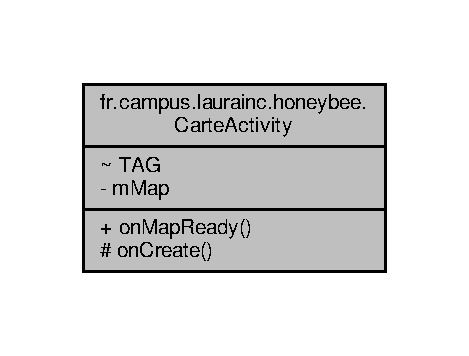
\includegraphics[width=225pt]{classfr_1_1campus_1_1laurainc_1_1honeybee_1_1_carte_activity__coll__graph}
\end{center}
\end{figure}
\subsubsection*{Fonctions membres publiques}
\begin{DoxyCompactItemize}
\item 
void \hyperlink{classfr_1_1campus_1_1laurainc_1_1honeybee_1_1_carte_activity_a30d970c7028be9de18778dbb19e65196}{on\+Map\+Ready} (Google\+Map google\+Map)
\end{DoxyCompactItemize}
\subsubsection*{Fonctions membres protégées}
\begin{DoxyCompactItemize}
\item 
void \hyperlink{classfr_1_1campus_1_1laurainc_1_1honeybee_1_1_carte_activity_a6e10bf7de1bf581b5118fa6de2ac465e}{on\+Create} (Bundle saved\+Instance\+State)
\end{DoxyCompactItemize}
\subsubsection*{Attributs privés}
\begin{DoxyCompactItemize}
\item 
Google\+Map \hyperlink{classfr_1_1campus_1_1laurainc_1_1honeybee_1_1_carte_activity_a101cebc8274b075aa3fee06ce55bf2fd}{m\+Map}
\end{DoxyCompactItemize}


\subsubsection{Documentation des fonctions membres}
\mbox{\Hypertarget{classfr_1_1campus_1_1laurainc_1_1honeybee_1_1_carte_activity_a6e10bf7de1bf581b5118fa6de2ac465e}\label{classfr_1_1campus_1_1laurainc_1_1honeybee_1_1_carte_activity_a6e10bf7de1bf581b5118fa6de2ac465e}} 
\index{fr\+::campus\+::laurainc\+::honeybee\+::\+Carte\+Activity@{fr\+::campus\+::laurainc\+::honeybee\+::\+Carte\+Activity}!on\+Create@{on\+Create}}
\index{on\+Create@{on\+Create}!fr\+::campus\+::laurainc\+::honeybee\+::\+Carte\+Activity@{fr\+::campus\+::laurainc\+::honeybee\+::\+Carte\+Activity}}
\paragraph{\texorpdfstring{on\+Create()}{onCreate()}}
{\footnotesize\ttfamily void fr.\+campus.\+laurainc.\+honeybee.\+Carte\+Activity.\+on\+Create (\begin{DoxyParamCaption}\item[{Bundle}]{saved\+Instance\+State }\end{DoxyParamCaption})\hspace{0.3cm}{\ttfamily [protected]}}


\begin{DoxyCode}
00033                                                        \{
00034         super.onCreate(savedInstanceState);
00035         setContentView(R.layout.activity\_carte);
00036 
00037 
00038         \textcolor{comment}{// Obtain the SupportMapFragment and get notified when the map is ready to be used.}
00039         SupportMapFragment mapFragment = (SupportMapFragment) getSupportFragmentManager()
00040                 .findFragmentById(R.id.map);
00041         mapFragment.getMapAsync(\textcolor{keyword}{this});
00042     \}
\end{DoxyCode}
\mbox{\Hypertarget{classfr_1_1campus_1_1laurainc_1_1honeybee_1_1_carte_activity_a30d970c7028be9de18778dbb19e65196}\label{classfr_1_1campus_1_1laurainc_1_1honeybee_1_1_carte_activity_a30d970c7028be9de18778dbb19e65196}} 
\index{fr\+::campus\+::laurainc\+::honeybee\+::\+Carte\+Activity@{fr\+::campus\+::laurainc\+::honeybee\+::\+Carte\+Activity}!on\+Map\+Ready@{on\+Map\+Ready}}
\index{on\+Map\+Ready@{on\+Map\+Ready}!fr\+::campus\+::laurainc\+::honeybee\+::\+Carte\+Activity@{fr\+::campus\+::laurainc\+::honeybee\+::\+Carte\+Activity}}
\paragraph{\texorpdfstring{on\+Map\+Ready()}{onMapReady()}}
{\footnotesize\ttfamily void fr.\+campus.\+laurainc.\+honeybee.\+Carte\+Activity.\+on\+Map\+Ready (\begin{DoxyParamCaption}\item[{Google\+Map}]{google\+Map }\end{DoxyParamCaption})}

Manipulates the map once available. This callback is triggered when the map is ready to be used. This is where we can add markers or lines, add listeners or move the camera. In this case, we just add a marker near Sydney, Australia. If Google Play services is not installed on the device, the user will be prompted to install it inside the Support\+Map\+Fragment. This method will only be triggered once the user has installed Google Play services and returned to the app. 
\begin{DoxyCode}
00055                                                 \{
00056         \hyperlink{classfr_1_1campus_1_1laurainc_1_1honeybee_1_1_carte_activity_a101cebc8274b075aa3fee06ce55bf2fd}{mMap} = googleMap;
00057 
00058         Intent intent = getIntent();
00059 
00060         \textcolor{keywordtype}{double} latitude = 0.0;
00061         \textcolor{keywordflow}{if} (intent.hasExtra(\textcolor{stringliteral}{"latitude"}))\{ \textcolor{comment}{// vérifie qu'une valeur est associée à la clé “edittext”}
00062             latitude = Double.parseDouble(intent.getStringExtra(\textcolor{stringliteral}{"latitude"}).replaceAll(\textcolor{stringliteral}{"°"}, \textcolor{stringliteral}{""})); \textcolor{comment}{// on
       récupère la valeur associée à la clé}
00063             Log.v(\textcolor{stringliteral}{"Map"}, \textcolor{stringliteral}{"Latitude :"} + valueOf(latitude));
00064         \}
00065 
00066         \textcolor{keywordtype}{double} longitude = 0.0;
00067         \textcolor{keywordflow}{if} (intent.hasExtra(\textcolor{stringliteral}{"longitude"}))\{ \textcolor{comment}{// vérifie qu'une valeur est associée à la clé “edittext”}
00068             longitude = Double.parseDouble(intent.getStringExtra(\textcolor{stringliteral}{"longitude"}).replaceAll(\textcolor{stringliteral}{"°"}, \textcolor{stringliteral}{""})); \textcolor{comment}{// on
       récupère la valeur associée à la clé}
00069             Log.v(\textcolor{stringliteral}{"Map"}, \textcolor{stringliteral}{"Longitude"} + valueOf(longitude));
00070         \}
00071 
00072         \textcolor{comment}{// Add a marker in Sydney and move the camera}
00073         LatLng sydney = \textcolor{keyword}{new} LatLng(latitude, longitude);
00074         \hyperlink{classfr_1_1campus_1_1laurainc_1_1honeybee_1_1_carte_activity_a101cebc8274b075aa3fee06ce55bf2fd}{mMap}.addMarker(\textcolor{keyword}{new} MarkerOptions().position(sydney).title(\textcolor{stringliteral}{"Ruche"}));
00075         \hyperlink{classfr_1_1campus_1_1laurainc_1_1honeybee_1_1_carte_activity_a101cebc8274b075aa3fee06ce55bf2fd}{mMap}.moveCamera(CameraUpdateFactory.newLatLng(sydney));
00076         \hyperlink{classfr_1_1campus_1_1laurainc_1_1honeybee_1_1_carte_activity_a101cebc8274b075aa3fee06ce55bf2fd}{mMap}.moveCamera(CameraUpdateFactory.newLatLngZoom(sydney, 15));
00077         \hyperlink{classfr_1_1campus_1_1laurainc_1_1honeybee_1_1_carte_activity_a101cebc8274b075aa3fee06ce55bf2fd}{mMap}.animateCamera(CameraUpdateFactory.zoomTo(10), 2000, null);
00078         Circle circle = \hyperlink{classfr_1_1campus_1_1laurainc_1_1honeybee_1_1_carte_activity_a101cebc8274b075aa3fee06ce55bf2fd}{mMap}.addCircle(\textcolor{keyword}{new} CircleOptions()
00079                 .center(\textcolor{keyword}{new} LatLng(latitude, longitude))
00080                 .radius(10000)
00081                 .strokeColor(Color.RED));
00082     \}
\end{DoxyCode}


\subsubsection{Documentation des données membres}
\mbox{\Hypertarget{classfr_1_1campus_1_1laurainc_1_1honeybee_1_1_carte_activity_a101cebc8274b075aa3fee06ce55bf2fd}\label{classfr_1_1campus_1_1laurainc_1_1honeybee_1_1_carte_activity_a101cebc8274b075aa3fee06ce55bf2fd}} 
\index{fr\+::campus\+::laurainc\+::honeybee\+::\+Carte\+Activity@{fr\+::campus\+::laurainc\+::honeybee\+::\+Carte\+Activity}!m\+Map@{m\+Map}}
\index{m\+Map@{m\+Map}!fr\+::campus\+::laurainc\+::honeybee\+::\+Carte\+Activity@{fr\+::campus\+::laurainc\+::honeybee\+::\+Carte\+Activity}}
\paragraph{\texorpdfstring{m\+Map}{mMap}}
{\footnotesize\ttfamily Google\+Map fr.\+campus.\+laurainc.\+honeybee.\+Carte\+Activity.\+m\+Map\hspace{0.3cm}{\ttfamily [private]}}



La documentation de cette classe a été générée à partir du fichier suivant \+:\begin{DoxyCompactItemize}
\item 
\hyperlink{_carte_activity_8java}{Carte\+Activity.\+java}\end{DoxyCompactItemize}

\hypertarget{classfr_1_1campus_1_1laurainc_1_1honeybee_1_1_client_m_q_t_t}{}\subsection{Référence de la classe fr.\+campus.\+laurainc.\+honeybee.\+Client\+M\+Q\+TT}
\label{classfr_1_1campus_1_1laurainc_1_1honeybee_1_1_client_m_q_t_t}\index{fr.\+campus.\+laurainc.\+honeybee.\+Client\+M\+Q\+TT@{fr.\+campus.\+laurainc.\+honeybee.\+Client\+M\+Q\+TT}}


Graphe de collaboration de fr.\+campus.\+laurainc.\+honeybee.\+Client\+M\+Q\+TT\+:\nopagebreak
\begin{figure}[H]
\begin{center}
\leavevmode
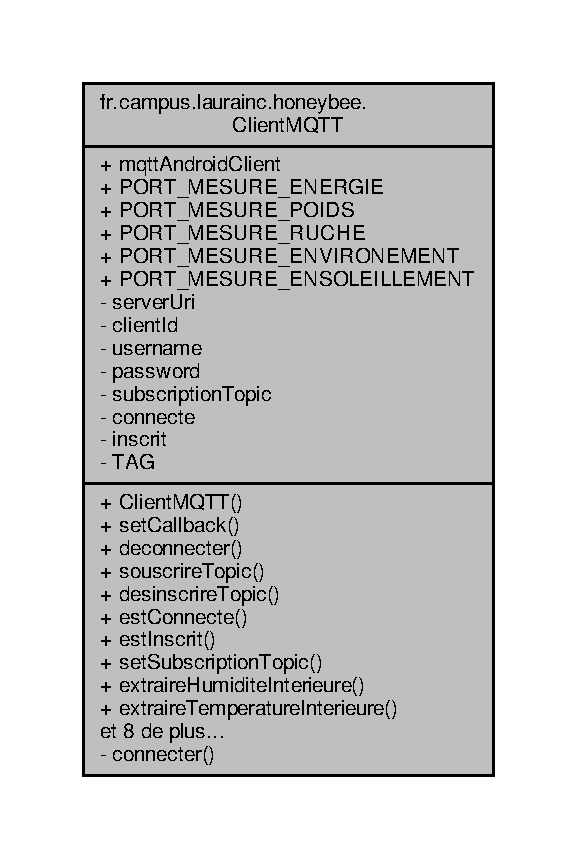
\includegraphics[width=277pt]{classfr_1_1campus_1_1laurainc_1_1honeybee_1_1_client_m_q_t_t__coll__graph}
\end{center}
\end{figure}
\subsubsection*{Fonctions membres publiques}
\begin{DoxyCompactItemize}
\item 
\hyperlink{classfr_1_1campus_1_1laurainc_1_1honeybee_1_1_client_m_q_t_t_a98cc7dce4cade9ffacfa462fe2f97088}{Client\+M\+Q\+TT} (String device\+ID, String topic, Context context)
\item 
void \hyperlink{classfr_1_1campus_1_1laurainc_1_1honeybee_1_1_client_m_q_t_t_ace2e0a1f888cb34e2a5a5c241eb6b94a}{set\+Callback} (Mqtt\+Callback\+Extended callback)
\item 
void \hyperlink{classfr_1_1campus_1_1laurainc_1_1honeybee_1_1_client_m_q_t_t_af067ec55e00ec18a14e248279872242f}{deconnecter} ()
\item 
void \hyperlink{classfr_1_1campus_1_1laurainc_1_1honeybee_1_1_client_m_q_t_t_a4c5ae1bb188b2f3c770ab6112b7d8590}{souscrire\+Topic} ()
\item 
void \hyperlink{classfr_1_1campus_1_1laurainc_1_1honeybee_1_1_client_m_q_t_t_aad5d88947bbdb3b83d4bf915985947e3}{desinscrire\+Topic} ()
\item 
boolean \hyperlink{classfr_1_1campus_1_1laurainc_1_1honeybee_1_1_client_m_q_t_t_a06c30a7291f526d0bd9a47fccb3ac1ad}{est\+Connecte} ()
\item 
boolean \hyperlink{classfr_1_1campus_1_1laurainc_1_1honeybee_1_1_client_m_q_t_t_a8ec5abba65d09f44e1c2c8f9ef652632}{est\+Inscrit} ()
\item 
void \hyperlink{classfr_1_1campus_1_1laurainc_1_1honeybee_1_1_client_m_q_t_t_af30038554905358c24a7226544822ff3}{set\+Subscription\+Topic} (String \hyperlink{classfr_1_1campus_1_1laurainc_1_1honeybee_1_1_client_m_q_t_t_a8771380740ea2e139b595f5b8fa7e0a5}{subscription\+Topic})
\item 
double \hyperlink{classfr_1_1campus_1_1laurainc_1_1honeybee_1_1_client_m_q_t_t_ad7fd3fa1a51a608646b146765cfc4546}{extraire\+Humidite\+Interieure} (Mqtt\+Message mqtt\+Message)
\item 
double \hyperlink{classfr_1_1campus_1_1laurainc_1_1honeybee_1_1_client_m_q_t_t_a92cd25872cdb04978a55ae166f858e0d}{extraire\+Temperature\+Interieure} (Mqtt\+Message mqtt\+Message)
\item 
int \hyperlink{classfr_1_1campus_1_1laurainc_1_1honeybee_1_1_client_m_q_t_t_a390da1e77f256fd9d90093bfec544b55}{extraire\+Poids} (Mqtt\+Message mqtt\+Message)
\item 
String \hyperlink{classfr_1_1campus_1_1laurainc_1_1honeybee_1_1_client_m_q_t_t_ace17d633909a5be8035518b9a6b528c2}{extraire\+Horodatage} (Mqtt\+Message mqtt\+Message)
\item 
double \hyperlink{classfr_1_1campus_1_1laurainc_1_1honeybee_1_1_client_m_q_t_t_a5f9be292aa0e594c2f555f29abbb4fc9}{extraire\+Temperature\+Exterieure} (Mqtt\+Message mqtt\+Message)
\item 
double \hyperlink{classfr_1_1campus_1_1laurainc_1_1honeybee_1_1_client_m_q_t_t_a0a3be0588498643af9098ab70a7a837a}{extraire\+Humidite\+Exterieure} (Mqtt\+Message mqtt\+Message)
\item 
double \hyperlink{classfr_1_1campus_1_1laurainc_1_1honeybee_1_1_client_m_q_t_t_a630a29e060e4a0c2891cd79fad8d3585}{extraire\+Pression} (Mqtt\+Message mqtt\+Message)
\item 
double \hyperlink{classfr_1_1campus_1_1laurainc_1_1honeybee_1_1_client_m_q_t_t_a38a76fc07a1793ba1a94898bdcd5ecbd}{extraire\+Ensoleillement} (Mqtt\+Message mqtt\+Message)
\item 
int \hyperlink{classfr_1_1campus_1_1laurainc_1_1honeybee_1_1_client_m_q_t_t_a93572795db92f79f417982f4785b71e0}{extraire\+Charge} (Mqtt\+Message mqtt\+Message)
\item 
double \hyperlink{classfr_1_1campus_1_1laurainc_1_1honeybee_1_1_client_m_q_t_t_a00ce9a2b07615c9337e452b5a51fedbe}{arrondir} (double nombre, double nb\+Apres\+Virgule)
\end{DoxyCompactItemize}
\subsubsection*{Attributs publics}
\begin{DoxyCompactItemize}
\item 
Mqtt\+Android\+Client \hyperlink{classfr_1_1campus_1_1laurainc_1_1honeybee_1_1_client_m_q_t_t_a587a9b6c785448cf3e37dc92bcac7961}{mqtt\+Android\+Client}
\end{DoxyCompactItemize}
\subsubsection*{Attributs publics statiques}
\begin{DoxyCompactItemize}
\item 
static final int \hyperlink{classfr_1_1campus_1_1laurainc_1_1honeybee_1_1_client_m_q_t_t_a423539a05c306ae52e5b6dc6fa6addc8}{P\+O\+R\+T\+\_\+\+M\+E\+S\+U\+R\+E\+\_\+\+E\+N\+E\+R\+G\+IE} = 1
\item 
static final int \hyperlink{classfr_1_1campus_1_1laurainc_1_1honeybee_1_1_client_m_q_t_t_a3630b0b9b902fee6796995399bee1a6a}{P\+O\+R\+T\+\_\+\+M\+E\+S\+U\+R\+E\+\_\+\+P\+O\+I\+DS} = 2
\item 
static final int \hyperlink{classfr_1_1campus_1_1laurainc_1_1honeybee_1_1_client_m_q_t_t_a3f264a8d2f3c294241bbe5557aa66770}{P\+O\+R\+T\+\_\+\+M\+E\+S\+U\+R\+E\+\_\+\+R\+U\+C\+HE} = 3
\item 
static final int \hyperlink{classfr_1_1campus_1_1laurainc_1_1honeybee_1_1_client_m_q_t_t_a85b9107442e2f5ef6fd6bef732336d8e}{P\+O\+R\+T\+\_\+\+M\+E\+S\+U\+R\+E\+\_\+\+E\+N\+V\+I\+R\+O\+N\+E\+M\+E\+NT} = 4
\item 
static final int \hyperlink{classfr_1_1campus_1_1laurainc_1_1honeybee_1_1_client_m_q_t_t_a49b4a61b3c65f6b3a1786ef6eeeb15e2}{P\+O\+R\+T\+\_\+\+M\+E\+S\+U\+R\+E\+\_\+\+E\+N\+S\+O\+L\+E\+I\+L\+L\+E\+M\+E\+NT} = 5
\end{DoxyCompactItemize}
\subsubsection*{Fonctions membres privées}
\begin{DoxyCompactItemize}
\item 
void \hyperlink{classfr_1_1campus_1_1laurainc_1_1honeybee_1_1_client_m_q_t_t_ab514adf6ebb879734ee8f2b3b2fd106a}{connecter} ()
\end{DoxyCompactItemize}
\subsubsection*{Attributs privés}
\begin{DoxyCompactItemize}
\item 
String \hyperlink{classfr_1_1campus_1_1laurainc_1_1honeybee_1_1_client_m_q_t_t_acc6543bf073de1b41fae396d8c0cf83d}{server\+Uri} = \char`\"{}tcp\+://eu.\+thethings.\+network\+:1883\char`\"{}
\item 
String \hyperlink{classfr_1_1campus_1_1laurainc_1_1honeybee_1_1_client_m_q_t_t_a18f8ff3e3e2ef132a4864b77bcfc009a}{client\+Id} = \char`\"{}mes\+\_\+ruches\char`\"{}
\item 
String \hyperlink{classfr_1_1campus_1_1laurainc_1_1honeybee_1_1_client_m_q_t_t_ab0ba59ea8b9ae85d9436fbd2e96d2e8a}{username} = \char`\"{}mes\+\_\+ruches\char`\"{}
\item 
String \hyperlink{classfr_1_1campus_1_1laurainc_1_1honeybee_1_1_client_m_q_t_t_a68fea868dcd85de576fb728aadcceed7}{password} = \char`\"{}ttn-\/account-\/v2.\+vC-\/aq\+M\+Rn\+L\+Lz\+Gk\+Nj\+O\+D\+Wgy81k\+Lqzx\+B\+P\+A\+T8\+\_\+mE-\/L7\+U2\+C\+\_\+w\char`\"{}
\item 
String \hyperlink{classfr_1_1campus_1_1laurainc_1_1honeybee_1_1_client_m_q_t_t_a8771380740ea2e139b595f5b8fa7e0a5}{subscription\+Topic}
\item 
boolean \hyperlink{classfr_1_1campus_1_1laurainc_1_1honeybee_1_1_client_m_q_t_t_abf92ba9ac98a707353748665a738c1c0}{connecte}
\item 
boolean \hyperlink{classfr_1_1campus_1_1laurainc_1_1honeybee_1_1_client_m_q_t_t_a774f2fd702c2a3581bf8dbfa341274fc}{inscrit}
\end{DoxyCompactItemize}
\subsubsection*{Attributs privés statiques}
\begin{DoxyCompactItemize}
\item 
static final String \hyperlink{classfr_1_1campus_1_1laurainc_1_1honeybee_1_1_client_m_q_t_t_a378324f705f8d7870c5f7be0cea02890}{T\+AG} = \char`\"{}Client\+M\+Q\+TT\char`\"{}
\begin{DoxyCompactList}\small\item\em le T\+AG de la classe pour les logs \end{DoxyCompactList}\end{DoxyCompactItemize}


\subsubsection{Documentation des constructeurs et destructeur}
\mbox{\Hypertarget{classfr_1_1campus_1_1laurainc_1_1honeybee_1_1_client_m_q_t_t_a98cc7dce4cade9ffacfa462fe2f97088}\label{classfr_1_1campus_1_1laurainc_1_1honeybee_1_1_client_m_q_t_t_a98cc7dce4cade9ffacfa462fe2f97088}} 
\index{fr\+::campus\+::laurainc\+::honeybee\+::\+Client\+M\+Q\+TT@{fr\+::campus\+::laurainc\+::honeybee\+::\+Client\+M\+Q\+TT}!Client\+M\+Q\+TT@{Client\+M\+Q\+TT}}
\index{Client\+M\+Q\+TT@{Client\+M\+Q\+TT}!fr\+::campus\+::laurainc\+::honeybee\+::\+Client\+M\+Q\+TT@{fr\+::campus\+::laurainc\+::honeybee\+::\+Client\+M\+Q\+TT}}
\paragraph{\texorpdfstring{Client\+M\+Q\+T\+T()}{ClientMQTT()}}
{\footnotesize\ttfamily fr.\+campus.\+laurainc.\+honeybee.\+Client\+M\+Q\+T\+T.\+Client\+M\+Q\+TT (\begin{DoxyParamCaption}\item[{String}]{device\+ID,  }\item[{String}]{topic,  }\item[{Context}]{context }\end{DoxyParamCaption})}



Références \hyperlink{classfr_1_1campus_1_1laurainc_1_1honeybee_1_1_client_m_q_t_t_ab514adf6ebb879734ee8f2b3b2fd106a}{fr.\+campus.\+laurainc.\+honeybee.\+Client\+M\+Q\+T\+T.\+connecter()}, et \hyperlink{classfr_1_1campus_1_1laurainc_1_1honeybee_1_1_client_m_q_t_t_af30038554905358c24a7226544822ff3}{fr.\+campus.\+laurainc.\+honeybee.\+Client\+M\+Q\+T\+T.\+set\+Subscription\+Topic()}.


\begin{DoxyCode}
00039     \{
00040         Log.v(\hyperlink{classfr_1_1campus_1_1laurainc_1_1honeybee_1_1_client_m_q_t_t_a378324f705f8d7870c5f7be0cea02890}{TAG}, \textcolor{stringliteral}{"deviceID : "} + deviceID + \textcolor{stringliteral}{" topic : "} + topic);
00041         \hyperlink{classfr_1_1campus_1_1laurainc_1_1honeybee_1_1_client_m_q_t_t_af30038554905358c24a7226544822ff3}{setSubscriptionTopic}(topic);
00042         \hyperlink{classfr_1_1campus_1_1laurainc_1_1honeybee_1_1_client_m_q_t_t_abf92ba9ac98a707353748665a738c1c0}{connecte} = \textcolor{keyword}{false};
00043         \hyperlink{classfr_1_1campus_1_1laurainc_1_1honeybee_1_1_client_m_q_t_t_a774f2fd702c2a3581bf8dbfa341274fc}{inscrit} = \textcolor{keyword}{false};
00044         \hyperlink{classfr_1_1campus_1_1laurainc_1_1honeybee_1_1_client_m_q_t_t_a587a9b6c785448cf3e37dc92bcac7961}{mqttAndroidClient} = \textcolor{keyword}{new} MqttAndroidClient(context, 
      \hyperlink{classfr_1_1campus_1_1laurainc_1_1honeybee_1_1_client_m_q_t_t_acc6543bf073de1b41fae396d8c0cf83d}{serverUri}, \hyperlink{classfr_1_1campus_1_1laurainc_1_1honeybee_1_1_client_m_q_t_t_a18f8ff3e3e2ef132a4864b77bcfc009a}{clientId});
00045         \hyperlink{classfr_1_1campus_1_1laurainc_1_1honeybee_1_1_client_m_q_t_t_a587a9b6c785448cf3e37dc92bcac7961}{mqttAndroidClient}.setCallback(\textcolor{keyword}{new} MqttCallbackExtended()
00046         \{
00047             @Override
00048             \textcolor{keyword}{public} \textcolor{keywordtype}{void} connectComplete(\textcolor{keywordtype}{boolean} b, String s) \{
00049                 Log.w(\hyperlink{classfr_1_1campus_1_1laurainc_1_1honeybee_1_1_client_m_q_t_t_a378324f705f8d7870c5f7be0cea02890}{TAG}, s);
00050             \}
00051 
00052             @Override
00053             \textcolor{keyword}{public} \textcolor{keywordtype}{void} connectionLost(Throwable throwable) \{
00054                 Log.w(\hyperlink{classfr_1_1campus_1_1laurainc_1_1honeybee_1_1_client_m_q_t_t_a378324f705f8d7870c5f7be0cea02890}{TAG}, \textcolor{stringliteral}{"Connexion perdue avec le serveur"});
00055                 \hyperlink{classfr_1_1campus_1_1laurainc_1_1honeybee_1_1_client_m_q_t_t_abf92ba9ac98a707353748665a738c1c0}{connecte} = \textcolor{keyword}{false};
00056             \}
00057 
00058             @Override
00059             \textcolor{keyword}{public} \textcolor{keywordtype}{void} messageArrived(String topic, MqttMessage mqttMessage) \textcolor{keywordflow}{throws} Exception \{
00060                 Log.w(\hyperlink{classfr_1_1campus_1_1laurainc_1_1honeybee_1_1_client_m_q_t_t_a378324f705f8d7870c5f7be0cea02890}{TAG}, mqttMessage.toString());
00061             \}
00062 
00063             @Override
00064             \textcolor{keyword}{public} \textcolor{keywordtype}{void} deliveryComplete(IMqttDeliveryToken iMqttDeliveryToken) \{Log.w(\textcolor{stringliteral}{"mqtt"}, \textcolor{stringliteral}{"Message
       envoyé"});\}
00065         \});
00066 
00067         \hyperlink{classfr_1_1campus_1_1laurainc_1_1honeybee_1_1_client_m_q_t_t_ab514adf6ebb879734ee8f2b3b2fd106a}{connecter}();
00068     \}
\end{DoxyCode}


\subsubsection{Documentation des fonctions membres}
\mbox{\Hypertarget{classfr_1_1campus_1_1laurainc_1_1honeybee_1_1_client_m_q_t_t_a00ce9a2b07615c9337e452b5a51fedbe}\label{classfr_1_1campus_1_1laurainc_1_1honeybee_1_1_client_m_q_t_t_a00ce9a2b07615c9337e452b5a51fedbe}} 
\index{fr\+::campus\+::laurainc\+::honeybee\+::\+Client\+M\+Q\+TT@{fr\+::campus\+::laurainc\+::honeybee\+::\+Client\+M\+Q\+TT}!arrondir@{arrondir}}
\index{arrondir@{arrondir}!fr\+::campus\+::laurainc\+::honeybee\+::\+Client\+M\+Q\+TT@{fr\+::campus\+::laurainc\+::honeybee\+::\+Client\+M\+Q\+TT}}
\paragraph{\texorpdfstring{arrondir()}{arrondir()}}
{\footnotesize\ttfamily double fr.\+campus.\+laurainc.\+honeybee.\+Client\+M\+Q\+T\+T.\+arrondir (\begin{DoxyParamCaption}\item[{double}]{nombre,  }\item[{double}]{nb\+Apres\+Virgule }\end{DoxyParamCaption})}



Référencé par \hyperlink{classfr_1_1campus_1_1laurainc_1_1honeybee_1_1_dashboard_activity_a13786896440cb102e03bd5ac4f54c3d8}{fr.\+campus.\+laurainc.\+honeybee.\+Dashboard\+Activity.\+afficher\+Poids()}.


\begin{DoxyCode}
00408     \{
00409         \textcolor{keywordflow}{return}(\textcolor{keywordtype}{double})((int)(nombre * Math.pow(10,nbApresVirgule) + .5)) / Math.pow(10,nbApresVirgule);
00410     \}
\end{DoxyCode}
\mbox{\Hypertarget{classfr_1_1campus_1_1laurainc_1_1honeybee_1_1_client_m_q_t_t_ab514adf6ebb879734ee8f2b3b2fd106a}\label{classfr_1_1campus_1_1laurainc_1_1honeybee_1_1_client_m_q_t_t_ab514adf6ebb879734ee8f2b3b2fd106a}} 
\index{fr\+::campus\+::laurainc\+::honeybee\+::\+Client\+M\+Q\+TT@{fr\+::campus\+::laurainc\+::honeybee\+::\+Client\+M\+Q\+TT}!connecter@{connecter}}
\index{connecter@{connecter}!fr\+::campus\+::laurainc\+::honeybee\+::\+Client\+M\+Q\+TT@{fr\+::campus\+::laurainc\+::honeybee\+::\+Client\+M\+Q\+TT}}
\paragraph{\texorpdfstring{connecter()}{connecter()}}
{\footnotesize\ttfamily void fr.\+campus.\+laurainc.\+honeybee.\+Client\+M\+Q\+T\+T.\+connecter (\begin{DoxyParamCaption}{ }\end{DoxyParamCaption})\hspace{0.3cm}{\ttfamily [private]}}



Références \hyperlink{classfr_1_1campus_1_1laurainc_1_1honeybee_1_1_client_m_q_t_t_a4c5ae1bb188b2f3c770ab6112b7d8590}{fr.\+campus.\+laurainc.\+honeybee.\+Client\+M\+Q\+T\+T.\+souscrire\+Topic()}.



Référencé par \hyperlink{classfr_1_1campus_1_1laurainc_1_1honeybee_1_1_client_m_q_t_t_a98cc7dce4cade9ffacfa462fe2f97088}{fr.\+campus.\+laurainc.\+honeybee.\+Client\+M\+Q\+T\+T.\+Client\+M\+Q\+T\+T()}.


\begin{DoxyCode}
00074                             \{
00075         MqttConnectOptions mqttConnectOptions = \textcolor{keyword}{new} MqttConnectOptions();
00076         mqttConnectOptions.setAutomaticReconnect(\textcolor{keyword}{true});
00077         mqttConnectOptions.setCleanSession(\textcolor{keyword}{false});
00078         mqttConnectOptions.setUserName(\hyperlink{classfr_1_1campus_1_1laurainc_1_1honeybee_1_1_client_m_q_t_t_ab0ba59ea8b9ae85d9436fbd2e96d2e8a}{username});
00079         mqttConnectOptions.setPassword(\hyperlink{classfr_1_1campus_1_1laurainc_1_1honeybee_1_1_client_m_q_t_t_a68fea868dcd85de576fb728aadcceed7}{password}.toCharArray());
00080 
00081         \textcolor{keywordflow}{try} \{
00082             Log.d(\hyperlink{classfr_1_1campus_1_1laurainc_1_1honeybee_1_1_client_m_q_t_t_a378324f705f8d7870c5f7be0cea02890}{TAG}, \textcolor{stringliteral}{"Connexion au serveur : "} + \hyperlink{classfr_1_1campus_1_1laurainc_1_1honeybee_1_1_client_m_q_t_t_acc6543bf073de1b41fae396d8c0cf83d}{serverUri});
00083             \hyperlink{classfr_1_1campus_1_1laurainc_1_1honeybee_1_1_client_m_q_t_t_a587a9b6c785448cf3e37dc92bcac7961}{mqttAndroidClient}.connect(mqttConnectOptions, null, \textcolor{keyword}{new} IMqttActionListener() 
      \{
00084                 @Override
00085                 \textcolor{keyword}{public} \textcolor{keywordtype}{void} onSuccess(IMqttToken asyncActionToken) \{
00086                     DisconnectedBufferOptions disconnectedBufferOptions = \textcolor{keyword}{new} DisconnectedBufferOptions();
00087                     disconnectedBufferOptions.setBufferEnabled(\textcolor{keyword}{true});
00088                     disconnectedBufferOptions.setBufferSize(100);
00089                     disconnectedBufferOptions.setPersistBuffer(\textcolor{keyword}{false});
00090                     disconnectedBufferOptions.setDeleteOldestMessages(\textcolor{keyword}{false});
00091                     \hyperlink{classfr_1_1campus_1_1laurainc_1_1honeybee_1_1_client_m_q_t_t_a587a9b6c785448cf3e37dc92bcac7961}{mqttAndroidClient}.setBufferOpts(disconnectedBufferOptions);
00092                     \hyperlink{classfr_1_1campus_1_1laurainc_1_1honeybee_1_1_client_m_q_t_t_abf92ba9ac98a707353748665a738c1c0}{connecte} = \textcolor{keyword}{true};
00093                     \hyperlink{classfr_1_1campus_1_1laurainc_1_1honeybee_1_1_client_m_q_t_t_a4c5ae1bb188b2f3c770ab6112b7d8590}{souscrireTopic}();
00094                     Log.d(\hyperlink{classfr_1_1campus_1_1laurainc_1_1honeybee_1_1_client_m_q_t_t_a378324f705f8d7870c5f7be0cea02890}{TAG}, \textcolor{stringliteral}{"Connecté au serveur : "} + \hyperlink{classfr_1_1campus_1_1laurainc_1_1honeybee_1_1_client_m_q_t_t_acc6543bf073de1b41fae396d8c0cf83d}{serverUri});
00095                 \}
00096 
00097                 @Override
00098                 \textcolor{keyword}{public} \textcolor{keywordtype}{void} onFailure(IMqttToken asyncActionToken, Throwable exception) \{
00099                     Log.d(\hyperlink{classfr_1_1campus_1_1laurainc_1_1honeybee_1_1_client_m_q_t_t_a378324f705f8d7870c5f7be0cea02890}{TAG}, \textcolor{stringliteral}{"Impossible de se connecter au serveur : "} + 
      \hyperlink{classfr_1_1campus_1_1laurainc_1_1honeybee_1_1_client_m_q_t_t_acc6543bf073de1b41fae396d8c0cf83d}{serverUri} + exception.toString());
00100                 \}
00101             \});
00102         \} \textcolor{keywordflow}{catch} (MqttException ex)\{
00103             ex.printStackTrace();
00104         \}
00105     \} \textcolor{comment}{// Méthode permettant de se connecter}
\end{DoxyCode}
\mbox{\Hypertarget{classfr_1_1campus_1_1laurainc_1_1honeybee_1_1_client_m_q_t_t_af067ec55e00ec18a14e248279872242f}\label{classfr_1_1campus_1_1laurainc_1_1honeybee_1_1_client_m_q_t_t_af067ec55e00ec18a14e248279872242f}} 
\index{fr\+::campus\+::laurainc\+::honeybee\+::\+Client\+M\+Q\+TT@{fr\+::campus\+::laurainc\+::honeybee\+::\+Client\+M\+Q\+TT}!deconnecter@{deconnecter}}
\index{deconnecter@{deconnecter}!fr\+::campus\+::laurainc\+::honeybee\+::\+Client\+M\+Q\+TT@{fr\+::campus\+::laurainc\+::honeybee\+::\+Client\+M\+Q\+TT}}
\paragraph{\texorpdfstring{deconnecter()}{deconnecter()}}
{\footnotesize\ttfamily void fr.\+campus.\+laurainc.\+honeybee.\+Client\+M\+Q\+T\+T.\+deconnecter (\begin{DoxyParamCaption}{ }\end{DoxyParamCaption})}



Références \hyperlink{classfr_1_1campus_1_1laurainc_1_1honeybee_1_1_client_m_q_t_t_aad5d88947bbdb3b83d4bf915985947e3}{fr.\+campus.\+laurainc.\+honeybee.\+Client\+M\+Q\+T\+T.\+desinscrire\+Topic()}, et \hyperlink{classfr_1_1campus_1_1laurainc_1_1honeybee_1_1_client_m_q_t_t_a8ec5abba65d09f44e1c2c8f9ef652632}{fr.\+campus.\+laurainc.\+honeybee.\+Client\+M\+Q\+T\+T.\+est\+Inscrit()}.



Référencé par \hyperlink{classfr_1_1campus_1_1laurainc_1_1honeybee_1_1_dashboard_activity_aeb7cdaf69c379e2b070e290130199543}{fr.\+campus.\+laurainc.\+honeybee.\+Dashboard\+Activity.\+afficher\+Liste\+Ruches()}.


\begin{DoxyCode}
00107                               \{
00108         \textcolor{keywordflow}{try} \{
00109             \textcolor{keywordflow}{if}(\hyperlink{classfr_1_1campus_1_1laurainc_1_1honeybee_1_1_client_m_q_t_t_a8ec5abba65d09f44e1c2c8f9ef652632}{estInscrit}())
00110                 \hyperlink{classfr_1_1campus_1_1laurainc_1_1honeybee_1_1_client_m_q_t_t_aad5d88947bbdb3b83d4bf915985947e3}{desinscrireTopic}();
00111 
00112             IMqttToken disconToken = \hyperlink{classfr_1_1campus_1_1laurainc_1_1honeybee_1_1_client_m_q_t_t_a587a9b6c785448cf3e37dc92bcac7961}{mqttAndroidClient}.disconnect();
00113             disconToken.setActionCallback(\textcolor{keyword}{new} IMqttActionListener() \{
00114                 @Override
00115                 \textcolor{keyword}{public} \textcolor{keywordtype}{void} onSuccess(IMqttToken asyncActionToken) \{
00116                     Log.d(\hyperlink{classfr_1_1campus_1_1laurainc_1_1honeybee_1_1_client_m_q_t_t_a378324f705f8d7870c5f7be0cea02890}{TAG}, \textcolor{stringliteral}{"Déconnecté du serveur : "} + \hyperlink{classfr_1_1campus_1_1laurainc_1_1honeybee_1_1_client_m_q_t_t_acc6543bf073de1b41fae396d8c0cf83d}{serverUri});
00117                     \hyperlink{classfr_1_1campus_1_1laurainc_1_1honeybee_1_1_client_m_q_t_t_abf92ba9ac98a707353748665a738c1c0}{connecte} = \textcolor{keyword}{false};
00118                 \}
00119 
00120                 @Override
00121                 \textcolor{keyword}{public} \textcolor{keywordtype}{void} onFailure(IMqttToken asyncActionToken, Throwable exception) \{
00122                     Log.d(\hyperlink{classfr_1_1campus_1_1laurainc_1_1honeybee_1_1_client_m_q_t_t_a378324f705f8d7870c5f7be0cea02890}{TAG}, \textcolor{stringliteral}{"Impossible de se déconnecter du serveur : "} + 
      \hyperlink{classfr_1_1campus_1_1laurainc_1_1honeybee_1_1_client_m_q_t_t_acc6543bf073de1b41fae396d8c0cf83d}{serverUri} + exception.toString());
00123                 \}
00124             \});
00125         \} \textcolor{keywordflow}{catch} (MqttException e) \{
00126             e.printStackTrace();
00127         \}
00128     \}
\end{DoxyCode}
\mbox{\Hypertarget{classfr_1_1campus_1_1laurainc_1_1honeybee_1_1_client_m_q_t_t_aad5d88947bbdb3b83d4bf915985947e3}\label{classfr_1_1campus_1_1laurainc_1_1honeybee_1_1_client_m_q_t_t_aad5d88947bbdb3b83d4bf915985947e3}} 
\index{fr\+::campus\+::laurainc\+::honeybee\+::\+Client\+M\+Q\+TT@{fr\+::campus\+::laurainc\+::honeybee\+::\+Client\+M\+Q\+TT}!desinscrire\+Topic@{desinscrire\+Topic}}
\index{desinscrire\+Topic@{desinscrire\+Topic}!fr\+::campus\+::laurainc\+::honeybee\+::\+Client\+M\+Q\+TT@{fr\+::campus\+::laurainc\+::honeybee\+::\+Client\+M\+Q\+TT}}
\paragraph{\texorpdfstring{desinscrire\+Topic()}{desinscrireTopic()}}
{\footnotesize\ttfamily void fr.\+campus.\+laurainc.\+honeybee.\+Client\+M\+Q\+T\+T.\+desinscrire\+Topic (\begin{DoxyParamCaption}{ }\end{DoxyParamCaption})}



Référencé par \hyperlink{classfr_1_1campus_1_1laurainc_1_1honeybee_1_1_client_m_q_t_t_af067ec55e00ec18a14e248279872242f}{fr.\+campus.\+laurainc.\+honeybee.\+Client\+M\+Q\+T\+T.\+deconnecter()}.


\begin{DoxyCode}
00152                                    \{
00153         \textcolor{keywordflow}{try} \{
00154             IMqttToken unsubToken = \hyperlink{classfr_1_1campus_1_1laurainc_1_1honeybee_1_1_client_m_q_t_t_a587a9b6c785448cf3e37dc92bcac7961}{mqttAndroidClient}.unsubscribe(
      \hyperlink{classfr_1_1campus_1_1laurainc_1_1honeybee_1_1_client_m_q_t_t_a8771380740ea2e139b595f5b8fa7e0a5}{subscriptionTopic});
00155             unsubToken.setActionCallback(\textcolor{keyword}{new} IMqttActionListener() \{
00156                 @Override
00157                 \textcolor{keyword}{public} \textcolor{keywordtype}{void} onSuccess(IMqttToken asyncActionToken) \{
00158                     Log.w(\hyperlink{classfr_1_1campus_1_1laurainc_1_1honeybee_1_1_client_m_q_t_t_a378324f705f8d7870c5f7be0cea02890}{TAG},\textcolor{stringliteral}{"Désabonné du topic "} + \hyperlink{classfr_1_1campus_1_1laurainc_1_1honeybee_1_1_client_m_q_t_t_a8771380740ea2e139b595f5b8fa7e0a5}{subscriptionTopic});
00159                     \hyperlink{classfr_1_1campus_1_1laurainc_1_1honeybee_1_1_client_m_q_t_t_a774f2fd702c2a3581bf8dbfa341274fc}{inscrit} = \textcolor{keyword}{false};
00160                 \}
00161 
00162                 @Override
00163                 \textcolor{keyword}{public} \textcolor{keywordtype}{void} onFailure(IMqttToken asyncActionToken, Throwable exception) \{
00164                     Log.w(\hyperlink{classfr_1_1campus_1_1laurainc_1_1honeybee_1_1_client_m_q_t_t_a378324f705f8d7870c5f7be0cea02890}{TAG}, \textcolor{stringliteral}{"Impossible de se désabonner du topic"});
00165                 \}
00166             \});
00167         \} \textcolor{keywordflow}{catch} (MqttException e) \{
00168             e.printStackTrace();
00169         \}
00170     \}
\end{DoxyCode}
\mbox{\Hypertarget{classfr_1_1campus_1_1laurainc_1_1honeybee_1_1_client_m_q_t_t_a06c30a7291f526d0bd9a47fccb3ac1ad}\label{classfr_1_1campus_1_1laurainc_1_1honeybee_1_1_client_m_q_t_t_a06c30a7291f526d0bd9a47fccb3ac1ad}} 
\index{fr\+::campus\+::laurainc\+::honeybee\+::\+Client\+M\+Q\+TT@{fr\+::campus\+::laurainc\+::honeybee\+::\+Client\+M\+Q\+TT}!est\+Connecte@{est\+Connecte}}
\index{est\+Connecte@{est\+Connecte}!fr\+::campus\+::laurainc\+::honeybee\+::\+Client\+M\+Q\+TT@{fr\+::campus\+::laurainc\+::honeybee\+::\+Client\+M\+Q\+TT}}
\paragraph{\texorpdfstring{est\+Connecte()}{estConnecte()}}
{\footnotesize\ttfamily boolean fr.\+campus.\+laurainc.\+honeybee.\+Client\+M\+Q\+T\+T.\+est\+Connecte (\begin{DoxyParamCaption}{ }\end{DoxyParamCaption})}



Références \hyperlink{classfr_1_1campus_1_1laurainc_1_1honeybee_1_1_client_m_q_t_t_abf92ba9ac98a707353748665a738c1c0}{fr.\+campus.\+laurainc.\+honeybee.\+Client\+M\+Q\+T\+T.\+connecte}.



Référencé par \hyperlink{classfr_1_1campus_1_1laurainc_1_1honeybee_1_1_dashboard_activity_aeb7cdaf69c379e2b070e290130199543}{fr.\+campus.\+laurainc.\+honeybee.\+Dashboard\+Activity.\+afficher\+Liste\+Ruches()}.


\begin{DoxyCode}
00172                                  \{
00173         Log.w(\hyperlink{classfr_1_1campus_1_1laurainc_1_1honeybee_1_1_client_m_q_t_t_a378324f705f8d7870c5f7be0cea02890}{TAG},\textcolor{stringliteral}{"isConnected "} + \hyperlink{classfr_1_1campus_1_1laurainc_1_1honeybee_1_1_client_m_q_t_t_a587a9b6c785448cf3e37dc92bcac7961}{mqttAndroidClient}.isConnected());
00174         Log.w(\hyperlink{classfr_1_1campus_1_1laurainc_1_1honeybee_1_1_client_m_q_t_t_a378324f705f8d7870c5f7be0cea02890}{TAG},\textcolor{stringliteral}{"connecte "} + \hyperlink{classfr_1_1campus_1_1laurainc_1_1honeybee_1_1_client_m_q_t_t_abf92ba9ac98a707353748665a738c1c0}{connecte});
00175         \textcolor{comment}{//return mqttAndroidClient.isConnected();}
00176         \textcolor{keywordflow}{return} \hyperlink{classfr_1_1campus_1_1laurainc_1_1honeybee_1_1_client_m_q_t_t_abf92ba9ac98a707353748665a738c1c0}{connecte};
00177     \}
\end{DoxyCode}
\mbox{\Hypertarget{classfr_1_1campus_1_1laurainc_1_1honeybee_1_1_client_m_q_t_t_a8ec5abba65d09f44e1c2c8f9ef652632}\label{classfr_1_1campus_1_1laurainc_1_1honeybee_1_1_client_m_q_t_t_a8ec5abba65d09f44e1c2c8f9ef652632}} 
\index{fr\+::campus\+::laurainc\+::honeybee\+::\+Client\+M\+Q\+TT@{fr\+::campus\+::laurainc\+::honeybee\+::\+Client\+M\+Q\+TT}!est\+Inscrit@{est\+Inscrit}}
\index{est\+Inscrit@{est\+Inscrit}!fr\+::campus\+::laurainc\+::honeybee\+::\+Client\+M\+Q\+TT@{fr\+::campus\+::laurainc\+::honeybee\+::\+Client\+M\+Q\+TT}}
\paragraph{\texorpdfstring{est\+Inscrit()}{estInscrit()}}
{\footnotesize\ttfamily boolean fr.\+campus.\+laurainc.\+honeybee.\+Client\+M\+Q\+T\+T.\+est\+Inscrit (\begin{DoxyParamCaption}{ }\end{DoxyParamCaption})}



Références \hyperlink{classfr_1_1campus_1_1laurainc_1_1honeybee_1_1_client_m_q_t_t_a774f2fd702c2a3581bf8dbfa341274fc}{fr.\+campus.\+laurainc.\+honeybee.\+Client\+M\+Q\+T\+T.\+inscrit}.



Référencé par \hyperlink{classfr_1_1campus_1_1laurainc_1_1honeybee_1_1_client_m_q_t_t_af067ec55e00ec18a14e248279872242f}{fr.\+campus.\+laurainc.\+honeybee.\+Client\+M\+Q\+T\+T.\+deconnecter()}.


\begin{DoxyCode}
00179                                 \{
00180         Log.w(\hyperlink{classfr_1_1campus_1_1laurainc_1_1honeybee_1_1_client_m_q_t_t_a378324f705f8d7870c5f7be0cea02890}{TAG},\textcolor{stringliteral}{"inscrit "} + \hyperlink{classfr_1_1campus_1_1laurainc_1_1honeybee_1_1_client_m_q_t_t_a774f2fd702c2a3581bf8dbfa341274fc}{inscrit});
00181         \textcolor{keywordflow}{return} \hyperlink{classfr_1_1campus_1_1laurainc_1_1honeybee_1_1_client_m_q_t_t_a774f2fd702c2a3581bf8dbfa341274fc}{inscrit};
00182     \}
\end{DoxyCode}
\mbox{\Hypertarget{classfr_1_1campus_1_1laurainc_1_1honeybee_1_1_client_m_q_t_t_a93572795db92f79f417982f4785b71e0}\label{classfr_1_1campus_1_1laurainc_1_1honeybee_1_1_client_m_q_t_t_a93572795db92f79f417982f4785b71e0}} 
\index{fr\+::campus\+::laurainc\+::honeybee\+::\+Client\+M\+Q\+TT@{fr\+::campus\+::laurainc\+::honeybee\+::\+Client\+M\+Q\+TT}!extraire\+Charge@{extraire\+Charge}}
\index{extraire\+Charge@{extraire\+Charge}!fr\+::campus\+::laurainc\+::honeybee\+::\+Client\+M\+Q\+TT@{fr\+::campus\+::laurainc\+::honeybee\+::\+Client\+M\+Q\+TT}}
\paragraph{\texorpdfstring{extraire\+Charge()}{extraireCharge()}}
{\footnotesize\ttfamily int fr.\+campus.\+laurainc.\+honeybee.\+Client\+M\+Q\+T\+T.\+extraire\+Charge (\begin{DoxyParamCaption}\item[{Mqtt\+Message}]{mqtt\+Message }\end{DoxyParamCaption})}



Références \hyperlink{classfr_1_1campus_1_1laurainc_1_1honeybee_1_1_client_m_q_t_t_ace17d633909a5be8035518b9a6b528c2}{fr.\+campus.\+laurainc.\+honeybee.\+Client\+M\+Q\+T\+T.\+extraire\+Horodatage()}.



Référencé par \hyperlink{classfr_1_1campus_1_1laurainc_1_1honeybee_1_1_dashboard_activity_a50d4c14e993ff1779ae5dce8cee11216}{fr.\+campus.\+laurainc.\+honeybee.\+Dashboard\+Activity.\+traiter\+Message()}.


\begin{DoxyCode}
00364     \{
00365         \textcolor{keyword}{final} String message = mqttMessage.toString();
00366         \textcolor{keywordtype}{int} charge = 0;
00367 
00368         \textcolor{keywordflow}{try}
00369         \{
00370             JSONObject jsonObjet = \textcolor{keyword}{new} JSONObject(message);
00371             JSONObject payloadFields = jsonObjet.getJSONObject(\textcolor{stringliteral}{"payload\_fields"});
00372             charge = payloadFields.getInt(\textcolor{stringliteral}{"charge"});
00373             Log.d(\hyperlink{classfr_1_1campus_1_1laurainc_1_1honeybee_1_1_client_m_q_t_t_a378324f705f8d7870c5f7be0cea02890}{TAG}, \textcolor{stringliteral}{"Charge : "} + charge + \textcolor{stringliteral}{" %"});
00374 
00375             \hyperlink{classfr_1_1campus_1_1laurainc_1_1honeybee_1_1_client_m_q_t_t_ace17d633909a5be8035518b9a6b528c2}{extraireHorodatage}(mqttMessage);
00376         \}
00377         \textcolor{keywordflow}{catch} (JSONException e)
00378         \{
00379             e.printStackTrace();
00380         \}
00381 
00382         \textcolor{keywordflow}{return}  charge;
00383     \}
\end{DoxyCode}
\mbox{\Hypertarget{classfr_1_1campus_1_1laurainc_1_1honeybee_1_1_client_m_q_t_t_a38a76fc07a1793ba1a94898bdcd5ecbd}\label{classfr_1_1campus_1_1laurainc_1_1honeybee_1_1_client_m_q_t_t_a38a76fc07a1793ba1a94898bdcd5ecbd}} 
\index{fr\+::campus\+::laurainc\+::honeybee\+::\+Client\+M\+Q\+TT@{fr\+::campus\+::laurainc\+::honeybee\+::\+Client\+M\+Q\+TT}!extraire\+Ensoleillement@{extraire\+Ensoleillement}}
\index{extraire\+Ensoleillement@{extraire\+Ensoleillement}!fr\+::campus\+::laurainc\+::honeybee\+::\+Client\+M\+Q\+TT@{fr\+::campus\+::laurainc\+::honeybee\+::\+Client\+M\+Q\+TT}}
\paragraph{\texorpdfstring{extraire\+Ensoleillement()}{extraireEnsoleillement()}}
{\footnotesize\ttfamily double fr.\+campus.\+laurainc.\+honeybee.\+Client\+M\+Q\+T\+T.\+extraire\+Ensoleillement (\begin{DoxyParamCaption}\item[{Mqtt\+Message}]{mqtt\+Message }\end{DoxyParamCaption})}



Références \hyperlink{classfr_1_1campus_1_1laurainc_1_1honeybee_1_1_client_m_q_t_t_ace17d633909a5be8035518b9a6b528c2}{fr.\+campus.\+laurainc.\+honeybee.\+Client\+M\+Q\+T\+T.\+extraire\+Horodatage()}.



Référencé par \hyperlink{classfr_1_1campus_1_1laurainc_1_1honeybee_1_1_dashboard_activity_a50d4c14e993ff1779ae5dce8cee11216}{fr.\+campus.\+laurainc.\+honeybee.\+Dashboard\+Activity.\+traiter\+Message()}.


\begin{DoxyCode}
00342     \{
00343         \textcolor{keyword}{final} String message = mqttMessage.toString();
00344         \textcolor{keywordtype}{double} ensoleillement = 0.;
00345 
00346         \textcolor{keywordflow}{try}
00347         \{
00348             JSONObject jsonObjet = \textcolor{keyword}{new} JSONObject(message);
00349             JSONObject payloadFields = jsonObjet.getJSONObject(\textcolor{stringliteral}{"payload\_fields"});
00350             ensoleillement = payloadFields.getDouble(\textcolor{stringliteral}{"ensoleillement"});
00351             Log.d(\hyperlink{classfr_1_1campus_1_1laurainc_1_1honeybee_1_1_client_m_q_t_t_a378324f705f8d7870c5f7be0cea02890}{TAG}, \textcolor{stringliteral}{"Ensoleillement : "} + ensoleillement + \textcolor{stringliteral}{" hPa"});
00352 
00353             \hyperlink{classfr_1_1campus_1_1laurainc_1_1honeybee_1_1_client_m_q_t_t_ace17d633909a5be8035518b9a6b528c2}{extraireHorodatage}(mqttMessage);
00354         \}
00355         \textcolor{keywordflow}{catch} (JSONException e)
00356         \{
00357             e.printStackTrace();
00358         \}
00359 
00360         \textcolor{keywordflow}{return}  ensoleillement;
00361     \}
\end{DoxyCode}
\mbox{\Hypertarget{classfr_1_1campus_1_1laurainc_1_1honeybee_1_1_client_m_q_t_t_ace17d633909a5be8035518b9a6b528c2}\label{classfr_1_1campus_1_1laurainc_1_1honeybee_1_1_client_m_q_t_t_ace17d633909a5be8035518b9a6b528c2}} 
\index{fr\+::campus\+::laurainc\+::honeybee\+::\+Client\+M\+Q\+TT@{fr\+::campus\+::laurainc\+::honeybee\+::\+Client\+M\+Q\+TT}!extraire\+Horodatage@{extraire\+Horodatage}}
\index{extraire\+Horodatage@{extraire\+Horodatage}!fr\+::campus\+::laurainc\+::honeybee\+::\+Client\+M\+Q\+TT@{fr\+::campus\+::laurainc\+::honeybee\+::\+Client\+M\+Q\+TT}}
\paragraph{\texorpdfstring{extraire\+Horodatage()}{extraireHorodatage()}}
{\footnotesize\ttfamily String fr.\+campus.\+laurainc.\+honeybee.\+Client\+M\+Q\+T\+T.\+extraire\+Horodatage (\begin{DoxyParamCaption}\item[{Mqtt\+Message}]{mqtt\+Message }\end{DoxyParamCaption})}



Référencé par \hyperlink{classfr_1_1campus_1_1laurainc_1_1honeybee_1_1_client_m_q_t_t_a93572795db92f79f417982f4785b71e0}{fr.\+campus.\+laurainc.\+honeybee.\+Client\+M\+Q\+T\+T.\+extraire\+Charge()}, \hyperlink{classfr_1_1campus_1_1laurainc_1_1honeybee_1_1_client_m_q_t_t_a38a76fc07a1793ba1a94898bdcd5ecbd}{fr.\+campus.\+laurainc.\+honeybee.\+Client\+M\+Q\+T\+T.\+extraire\+Ensoleillement()}, \hyperlink{classfr_1_1campus_1_1laurainc_1_1honeybee_1_1_client_m_q_t_t_a0a3be0588498643af9098ab70a7a837a}{fr.\+campus.\+laurainc.\+honeybee.\+Client\+M\+Q\+T\+T.\+extraire\+Humidite\+Exterieure()}, \hyperlink{classfr_1_1campus_1_1laurainc_1_1honeybee_1_1_client_m_q_t_t_ad7fd3fa1a51a608646b146765cfc4546}{fr.\+campus.\+laurainc.\+honeybee.\+Client\+M\+Q\+T\+T.\+extraire\+Humidite\+Interieure()}, \hyperlink{classfr_1_1campus_1_1laurainc_1_1honeybee_1_1_client_m_q_t_t_a390da1e77f256fd9d90093bfec544b55}{fr.\+campus.\+laurainc.\+honeybee.\+Client\+M\+Q\+T\+T.\+extraire\+Poids()}, \hyperlink{classfr_1_1campus_1_1laurainc_1_1honeybee_1_1_client_m_q_t_t_a630a29e060e4a0c2891cd79fad8d3585}{fr.\+campus.\+laurainc.\+honeybee.\+Client\+M\+Q\+T\+T.\+extraire\+Pression()}, \hyperlink{classfr_1_1campus_1_1laurainc_1_1honeybee_1_1_client_m_q_t_t_a5f9be292aa0e594c2f555f29abbb4fc9}{fr.\+campus.\+laurainc.\+honeybee.\+Client\+M\+Q\+T\+T.\+extraire\+Temperature\+Exterieure()}, \hyperlink{classfr_1_1campus_1_1laurainc_1_1honeybee_1_1_client_m_q_t_t_a92cd25872cdb04978a55ae166f858e0d}{fr.\+campus.\+laurainc.\+honeybee.\+Client\+M\+Q\+T\+T.\+extraire\+Temperature\+Interieure()}, et \hyperlink{classfr_1_1campus_1_1laurainc_1_1honeybee_1_1_dashboard_activity_a50d4c14e993ff1779ae5dce8cee11216}{fr.\+campus.\+laurainc.\+honeybee.\+Dashboard\+Activity.\+traiter\+Message()}.


\begin{DoxyCode}
00255     \{
00256         \textcolor{keyword}{final} String message = mqttMessage.toString();
00257         String date = \textcolor{stringliteral}{""};
00258 
00259         \textcolor{keywordflow}{try}
00260         \{
00261             JSONObject jsonObject = \textcolor{keyword}{new} JSONObject(message);
00262             date = jsonObject.getJSONObject(\textcolor{stringliteral}{"metadata"}).getString(\textcolor{stringliteral}{"time"});
00263             date = date.substring(0, 10) + \textcolor{stringliteral}{" "} + date.substring(11, 19);
00264             Log.d(\hyperlink{classfr_1_1campus_1_1laurainc_1_1honeybee_1_1_client_m_q_t_t_a378324f705f8d7870c5f7be0cea02890}{TAG}, \textcolor{stringliteral}{"Horodatage : "} + date);
00265 
00266         \}
00267         \textcolor{keywordflow}{catch} (JSONException e)
00268         \{
00269             e.printStackTrace();
00270         \}
00271 
00272         \textcolor{keywordflow}{return}  date;
00273     \}
\end{DoxyCode}
\mbox{\Hypertarget{classfr_1_1campus_1_1laurainc_1_1honeybee_1_1_client_m_q_t_t_a0a3be0588498643af9098ab70a7a837a}\label{classfr_1_1campus_1_1laurainc_1_1honeybee_1_1_client_m_q_t_t_a0a3be0588498643af9098ab70a7a837a}} 
\index{fr\+::campus\+::laurainc\+::honeybee\+::\+Client\+M\+Q\+TT@{fr\+::campus\+::laurainc\+::honeybee\+::\+Client\+M\+Q\+TT}!extraire\+Humidite\+Exterieure@{extraire\+Humidite\+Exterieure}}
\index{extraire\+Humidite\+Exterieure@{extraire\+Humidite\+Exterieure}!fr\+::campus\+::laurainc\+::honeybee\+::\+Client\+M\+Q\+TT@{fr\+::campus\+::laurainc\+::honeybee\+::\+Client\+M\+Q\+TT}}
\paragraph{\texorpdfstring{extraire\+Humidite\+Exterieure()}{extraireHumiditeExterieure()}}
{\footnotesize\ttfamily double fr.\+campus.\+laurainc.\+honeybee.\+Client\+M\+Q\+T\+T.\+extraire\+Humidite\+Exterieure (\begin{DoxyParamCaption}\item[{Mqtt\+Message}]{mqtt\+Message }\end{DoxyParamCaption})}



Références \hyperlink{classfr_1_1campus_1_1laurainc_1_1honeybee_1_1_client_m_q_t_t_ace17d633909a5be8035518b9a6b528c2}{fr.\+campus.\+laurainc.\+honeybee.\+Client\+M\+Q\+T\+T.\+extraire\+Horodatage()}.



Référencé par \hyperlink{classfr_1_1campus_1_1laurainc_1_1honeybee_1_1_dashboard_activity_a50d4c14e993ff1779ae5dce8cee11216}{fr.\+campus.\+laurainc.\+honeybee.\+Dashboard\+Activity.\+traiter\+Message()}.


\begin{DoxyCode}
00298     \{
00299         \textcolor{keyword}{final} String message = mqttMessage.toString();
00300         \textcolor{keywordtype}{double} humiditeExterieure = 0.;
00301 
00302         \textcolor{keywordflow}{try}
00303         \{
00304             JSONObject jsonObjet = \textcolor{keyword}{new} JSONObject(message);
00305             JSONObject payloadFields = jsonObjet.getJSONObject(\textcolor{stringliteral}{"payload\_fields"});
00306             humiditeExterieure = payloadFields.getDouble(\textcolor{stringliteral}{"humidite"});
00307             Log.d(\hyperlink{classfr_1_1campus_1_1laurainc_1_1honeybee_1_1_client_m_q_t_t_a378324f705f8d7870c5f7be0cea02890}{TAG}, \textcolor{stringliteral}{"Humidité extérieure : "} + humiditeExterieure + \textcolor{stringliteral}{" %"});
00308 
00309             \hyperlink{classfr_1_1campus_1_1laurainc_1_1honeybee_1_1_client_m_q_t_t_ace17d633909a5be8035518b9a6b528c2}{extraireHorodatage}(mqttMessage);
00310         \}
00311         \textcolor{keywordflow}{catch} (JSONException e)
00312         \{
00313             e.printStackTrace();
00314         \}
00315 
00316         \textcolor{keywordflow}{return}  humiditeExterieure;
00317     \}
\end{DoxyCode}
\mbox{\Hypertarget{classfr_1_1campus_1_1laurainc_1_1honeybee_1_1_client_m_q_t_t_ad7fd3fa1a51a608646b146765cfc4546}\label{classfr_1_1campus_1_1laurainc_1_1honeybee_1_1_client_m_q_t_t_ad7fd3fa1a51a608646b146765cfc4546}} 
\index{fr\+::campus\+::laurainc\+::honeybee\+::\+Client\+M\+Q\+TT@{fr\+::campus\+::laurainc\+::honeybee\+::\+Client\+M\+Q\+TT}!extraire\+Humidite\+Interieure@{extraire\+Humidite\+Interieure}}
\index{extraire\+Humidite\+Interieure@{extraire\+Humidite\+Interieure}!fr\+::campus\+::laurainc\+::honeybee\+::\+Client\+M\+Q\+TT@{fr\+::campus\+::laurainc\+::honeybee\+::\+Client\+M\+Q\+TT}}
\paragraph{\texorpdfstring{extraire\+Humidite\+Interieure()}{extraireHumiditeInterieure()}}
{\footnotesize\ttfamily double fr.\+campus.\+laurainc.\+honeybee.\+Client\+M\+Q\+T\+T.\+extraire\+Humidite\+Interieure (\begin{DoxyParamCaption}\item[{Mqtt\+Message}]{mqtt\+Message }\end{DoxyParamCaption})}



Références \hyperlink{classfr_1_1campus_1_1laurainc_1_1honeybee_1_1_client_m_q_t_t_ace17d633909a5be8035518b9a6b528c2}{fr.\+campus.\+laurainc.\+honeybee.\+Client\+M\+Q\+T\+T.\+extraire\+Horodatage()}.



Référencé par \hyperlink{classfr_1_1campus_1_1laurainc_1_1honeybee_1_1_dashboard_activity_a50d4c14e993ff1779ae5dce8cee11216}{fr.\+campus.\+laurainc.\+honeybee.\+Dashboard\+Activity.\+traiter\+Message()}.


\begin{DoxyCode}
00189     \{
00190         \textcolor{keyword}{final} String message = mqttMessage.toString();
00191         \textcolor{keywordtype}{double} humidite = 0.;
00192 
00193         \textcolor{keywordflow}{try}
00194         \{
00195             JSONObject jsonObjet = \textcolor{keyword}{new} JSONObject(message);
00196             JSONObject payloadFields = jsonObjet.getJSONObject(\textcolor{stringliteral}{"payload\_fields"});
00197             humidite = payloadFields.getDouble(\textcolor{stringliteral}{"humidite"});
00198             Log.d(\hyperlink{classfr_1_1campus_1_1laurainc_1_1honeybee_1_1_client_m_q_t_t_a378324f705f8d7870c5f7be0cea02890}{TAG}, \textcolor{stringliteral}{"Humidite intérieure : "} + humidite + \textcolor{stringliteral}{" %"});
00199 
00200             \hyperlink{classfr_1_1campus_1_1laurainc_1_1honeybee_1_1_client_m_q_t_t_ace17d633909a5be8035518b9a6b528c2}{extraireHorodatage}(mqttMessage);
00201         \}
00202         \textcolor{keywordflow}{catch} (JSONException e)
00203         \{
00204             e.printStackTrace();
00205         \}
00206 
00207         \textcolor{keywordflow}{return} humidite;
00208     \}
\end{DoxyCode}
\mbox{\Hypertarget{classfr_1_1campus_1_1laurainc_1_1honeybee_1_1_client_m_q_t_t_a390da1e77f256fd9d90093bfec544b55}\label{classfr_1_1campus_1_1laurainc_1_1honeybee_1_1_client_m_q_t_t_a390da1e77f256fd9d90093bfec544b55}} 
\index{fr\+::campus\+::laurainc\+::honeybee\+::\+Client\+M\+Q\+TT@{fr\+::campus\+::laurainc\+::honeybee\+::\+Client\+M\+Q\+TT}!extraire\+Poids@{extraire\+Poids}}
\index{extraire\+Poids@{extraire\+Poids}!fr\+::campus\+::laurainc\+::honeybee\+::\+Client\+M\+Q\+TT@{fr\+::campus\+::laurainc\+::honeybee\+::\+Client\+M\+Q\+TT}}
\paragraph{\texorpdfstring{extraire\+Poids()}{extrairePoids()}}
{\footnotesize\ttfamily int fr.\+campus.\+laurainc.\+honeybee.\+Client\+M\+Q\+T\+T.\+extraire\+Poids (\begin{DoxyParamCaption}\item[{Mqtt\+Message}]{mqtt\+Message }\end{DoxyParamCaption})}



Références \hyperlink{classfr_1_1campus_1_1laurainc_1_1honeybee_1_1_client_m_q_t_t_ace17d633909a5be8035518b9a6b528c2}{fr.\+campus.\+laurainc.\+honeybee.\+Client\+M\+Q\+T\+T.\+extraire\+Horodatage()}.



Référencé par \hyperlink{classfr_1_1campus_1_1laurainc_1_1honeybee_1_1_dashboard_activity_a50d4c14e993ff1779ae5dce8cee11216}{fr.\+campus.\+laurainc.\+honeybee.\+Dashboard\+Activity.\+traiter\+Message()}.


\begin{DoxyCode}
00233     \{
00234         \textcolor{keyword}{final} String message = mqttMessage.toString();
00235         \textcolor{keywordtype}{int} poids = 0;
00236 
00237         \textcolor{keywordflow}{try}
00238         \{
00239             JSONObject jsonObjet = \textcolor{keyword}{new} JSONObject(message);
00240             JSONObject payloadFields = jsonObjet.getJSONObject(\textcolor{stringliteral}{"payload\_fields"});
00241             poids = payloadFields.getInt(\textcolor{stringliteral}{"poids"});
00242             Log.d(\hyperlink{classfr_1_1campus_1_1laurainc_1_1honeybee_1_1_client_m_q_t_t_a378324f705f8d7870c5f7be0cea02890}{TAG}, \textcolor{stringliteral}{"Poids : "} + poids + \textcolor{stringliteral}{" Kg"});
00243 
00244             \hyperlink{classfr_1_1campus_1_1laurainc_1_1honeybee_1_1_client_m_q_t_t_ace17d633909a5be8035518b9a6b528c2}{extraireHorodatage}(mqttMessage);
00245         \}
00246         \textcolor{keywordflow}{catch} (JSONException e)
00247         \{
00248             e.printStackTrace();
00249         \}
00250 
00251         \textcolor{keywordflow}{return} poids;
00252     \}
\end{DoxyCode}
\mbox{\Hypertarget{classfr_1_1campus_1_1laurainc_1_1honeybee_1_1_client_m_q_t_t_a630a29e060e4a0c2891cd79fad8d3585}\label{classfr_1_1campus_1_1laurainc_1_1honeybee_1_1_client_m_q_t_t_a630a29e060e4a0c2891cd79fad8d3585}} 
\index{fr\+::campus\+::laurainc\+::honeybee\+::\+Client\+M\+Q\+TT@{fr\+::campus\+::laurainc\+::honeybee\+::\+Client\+M\+Q\+TT}!extraire\+Pression@{extraire\+Pression}}
\index{extraire\+Pression@{extraire\+Pression}!fr\+::campus\+::laurainc\+::honeybee\+::\+Client\+M\+Q\+TT@{fr\+::campus\+::laurainc\+::honeybee\+::\+Client\+M\+Q\+TT}}
\paragraph{\texorpdfstring{extraire\+Pression()}{extrairePression()}}
{\footnotesize\ttfamily double fr.\+campus.\+laurainc.\+honeybee.\+Client\+M\+Q\+T\+T.\+extraire\+Pression (\begin{DoxyParamCaption}\item[{Mqtt\+Message}]{mqtt\+Message }\end{DoxyParamCaption})}



Références \hyperlink{classfr_1_1campus_1_1laurainc_1_1honeybee_1_1_client_m_q_t_t_ace17d633909a5be8035518b9a6b528c2}{fr.\+campus.\+laurainc.\+honeybee.\+Client\+M\+Q\+T\+T.\+extraire\+Horodatage()}.



Référencé par \hyperlink{classfr_1_1campus_1_1laurainc_1_1honeybee_1_1_dashboard_activity_a50d4c14e993ff1779ae5dce8cee11216}{fr.\+campus.\+laurainc.\+honeybee.\+Dashboard\+Activity.\+traiter\+Message()}.


\begin{DoxyCode}
00320     \{
00321         \textcolor{keyword}{final} String message = mqttMessage.toString();
00322         \textcolor{keywordtype}{double} pression = 0.;
00323 
00324         \textcolor{keywordflow}{try}
00325         \{
00326             JSONObject jsonObjet = \textcolor{keyword}{new} JSONObject(message);
00327             JSONObject payloadFields = jsonObjet.getJSONObject(\textcolor{stringliteral}{"payload\_fields"});
00328             pression = payloadFields.getDouble(\textcolor{stringliteral}{"pression"});
00329             Log.d(\hyperlink{classfr_1_1campus_1_1laurainc_1_1honeybee_1_1_client_m_q_t_t_a378324f705f8d7870c5f7be0cea02890}{TAG}, \textcolor{stringliteral}{"Pression : "} + pression + \textcolor{stringliteral}{" hPa"});
00330 
00331             \hyperlink{classfr_1_1campus_1_1laurainc_1_1honeybee_1_1_client_m_q_t_t_ace17d633909a5be8035518b9a6b528c2}{extraireHorodatage}(mqttMessage);
00332         \}
00333         \textcolor{keywordflow}{catch} (JSONException e)
00334         \{
00335             e.printStackTrace();
00336         \}
00337 
00338         \textcolor{keywordflow}{return}  pression;
00339     \}
\end{DoxyCode}
\mbox{\Hypertarget{classfr_1_1campus_1_1laurainc_1_1honeybee_1_1_client_m_q_t_t_a5f9be292aa0e594c2f555f29abbb4fc9}\label{classfr_1_1campus_1_1laurainc_1_1honeybee_1_1_client_m_q_t_t_a5f9be292aa0e594c2f555f29abbb4fc9}} 
\index{fr\+::campus\+::laurainc\+::honeybee\+::\+Client\+M\+Q\+TT@{fr\+::campus\+::laurainc\+::honeybee\+::\+Client\+M\+Q\+TT}!extraire\+Temperature\+Exterieure@{extraire\+Temperature\+Exterieure}}
\index{extraire\+Temperature\+Exterieure@{extraire\+Temperature\+Exterieure}!fr\+::campus\+::laurainc\+::honeybee\+::\+Client\+M\+Q\+TT@{fr\+::campus\+::laurainc\+::honeybee\+::\+Client\+M\+Q\+TT}}
\paragraph{\texorpdfstring{extraire\+Temperature\+Exterieure()}{extraireTemperatureExterieure()}}
{\footnotesize\ttfamily double fr.\+campus.\+laurainc.\+honeybee.\+Client\+M\+Q\+T\+T.\+extraire\+Temperature\+Exterieure (\begin{DoxyParamCaption}\item[{Mqtt\+Message}]{mqtt\+Message }\end{DoxyParamCaption})}



Références \hyperlink{classfr_1_1campus_1_1laurainc_1_1honeybee_1_1_client_m_q_t_t_ace17d633909a5be8035518b9a6b528c2}{fr.\+campus.\+laurainc.\+honeybee.\+Client\+M\+Q\+T\+T.\+extraire\+Horodatage()}.



Référencé par \hyperlink{classfr_1_1campus_1_1laurainc_1_1honeybee_1_1_dashboard_activity_a50d4c14e993ff1779ae5dce8cee11216}{fr.\+campus.\+laurainc.\+honeybee.\+Dashboard\+Activity.\+traiter\+Message()}.


\begin{DoxyCode}
00276     \{
00277         \textcolor{keyword}{final} String message = mqttMessage.toString();
00278         \textcolor{keywordtype}{double} temperatureExterieure = 0.;
00279 
00280         \textcolor{keywordflow}{try}
00281         \{
00282             JSONObject jsonObjet = \textcolor{keyword}{new} JSONObject(message);
00283             JSONObject payloadFields = jsonObjet.getJSONObject(\textcolor{stringliteral}{"payload\_fields"});
00284             temperatureExterieure = payloadFields.getDouble(\textcolor{stringliteral}{"temperature"});
00285             Log.d(\hyperlink{classfr_1_1campus_1_1laurainc_1_1honeybee_1_1_client_m_q_t_t_a378324f705f8d7870c5f7be0cea02890}{TAG}, \textcolor{stringliteral}{"Temperature extérieure : "} + temperatureExterieure + \textcolor{stringliteral}{" °C"});
00286 
00287             \hyperlink{classfr_1_1campus_1_1laurainc_1_1honeybee_1_1_client_m_q_t_t_ace17d633909a5be8035518b9a6b528c2}{extraireHorodatage}(mqttMessage);
00288         \}
00289         \textcolor{keywordflow}{catch} (JSONException e)
00290         \{
00291             e.printStackTrace();
00292         \}
00293 
00294         \textcolor{keywordflow}{return}  temperatureExterieure;
00295     \}
\end{DoxyCode}
\mbox{\Hypertarget{classfr_1_1campus_1_1laurainc_1_1honeybee_1_1_client_m_q_t_t_a92cd25872cdb04978a55ae166f858e0d}\label{classfr_1_1campus_1_1laurainc_1_1honeybee_1_1_client_m_q_t_t_a92cd25872cdb04978a55ae166f858e0d}} 
\index{fr\+::campus\+::laurainc\+::honeybee\+::\+Client\+M\+Q\+TT@{fr\+::campus\+::laurainc\+::honeybee\+::\+Client\+M\+Q\+TT}!extraire\+Temperature\+Interieure@{extraire\+Temperature\+Interieure}}
\index{extraire\+Temperature\+Interieure@{extraire\+Temperature\+Interieure}!fr\+::campus\+::laurainc\+::honeybee\+::\+Client\+M\+Q\+TT@{fr\+::campus\+::laurainc\+::honeybee\+::\+Client\+M\+Q\+TT}}
\paragraph{\texorpdfstring{extraire\+Temperature\+Interieure()}{extraireTemperatureInterieure()}}
{\footnotesize\ttfamily double fr.\+campus.\+laurainc.\+honeybee.\+Client\+M\+Q\+T\+T.\+extraire\+Temperature\+Interieure (\begin{DoxyParamCaption}\item[{Mqtt\+Message}]{mqtt\+Message }\end{DoxyParamCaption})}



Références \hyperlink{classfr_1_1campus_1_1laurainc_1_1honeybee_1_1_client_m_q_t_t_ace17d633909a5be8035518b9a6b528c2}{fr.\+campus.\+laurainc.\+honeybee.\+Client\+M\+Q\+T\+T.\+extraire\+Horodatage()}.



Référencé par \hyperlink{classfr_1_1campus_1_1laurainc_1_1honeybee_1_1_dashboard_activity_a50d4c14e993ff1779ae5dce8cee11216}{fr.\+campus.\+laurainc.\+honeybee.\+Dashboard\+Activity.\+traiter\+Message()}.


\begin{DoxyCode}
00211     \{
00212         \textcolor{keyword}{final} String message = mqttMessage.toString();
00213         \textcolor{keywordtype}{double} temperature = 0.;
00214 
00215         \textcolor{keywordflow}{try}
00216         \{
00217             JSONObject jsonObjet = \textcolor{keyword}{new} JSONObject(message);
00218             JSONObject payloadFields = jsonObjet.getJSONObject(\textcolor{stringliteral}{"payload\_fields"});
00219             temperature = payloadFields.getDouble(\textcolor{stringliteral}{"temperature"});
00220             Log.d(\hyperlink{classfr_1_1campus_1_1laurainc_1_1honeybee_1_1_client_m_q_t_t_a378324f705f8d7870c5f7be0cea02890}{TAG}, \textcolor{stringliteral}{"Température : "} + temperature + \textcolor{stringliteral}{" °C"});
00221 
00222             \hyperlink{classfr_1_1campus_1_1laurainc_1_1honeybee_1_1_client_m_q_t_t_ace17d633909a5be8035518b9a6b528c2}{extraireHorodatage}(mqttMessage);
00223         \}
00224         \textcolor{keywordflow}{catch} (JSONException e)
00225         \{
00226             e.printStackTrace();
00227         \}
00228 
00229         \textcolor{keywordflow}{return} temperature;
00230     \}
\end{DoxyCode}
\mbox{\Hypertarget{classfr_1_1campus_1_1laurainc_1_1honeybee_1_1_client_m_q_t_t_ace2e0a1f888cb34e2a5a5c241eb6b94a}\label{classfr_1_1campus_1_1laurainc_1_1honeybee_1_1_client_m_q_t_t_ace2e0a1f888cb34e2a5a5c241eb6b94a}} 
\index{fr\+::campus\+::laurainc\+::honeybee\+::\+Client\+M\+Q\+TT@{fr\+::campus\+::laurainc\+::honeybee\+::\+Client\+M\+Q\+TT}!set\+Callback@{set\+Callback}}
\index{set\+Callback@{set\+Callback}!fr\+::campus\+::laurainc\+::honeybee\+::\+Client\+M\+Q\+TT@{fr\+::campus\+::laurainc\+::honeybee\+::\+Client\+M\+Q\+TT}}
\paragraph{\texorpdfstring{set\+Callback()}{setCallback()}}
{\footnotesize\ttfamily void fr.\+campus.\+laurainc.\+honeybee.\+Client\+M\+Q\+T\+T.\+set\+Callback (\begin{DoxyParamCaption}\item[{Mqtt\+Callback\+Extended}]{callback }\end{DoxyParamCaption})}



Référencé par \hyperlink{classfr_1_1campus_1_1laurainc_1_1honeybee_1_1_dashboard_activity_abfefd572745e1034a025bc836812ae4f}{fr.\+campus.\+laurainc.\+honeybee.\+Dashboard\+Activity.\+communiquer\+T\+T\+N()}.


\begin{DoxyCode}
00070                                                            \{
00071         \hyperlink{classfr_1_1campus_1_1laurainc_1_1honeybee_1_1_client_m_q_t_t_a587a9b6c785448cf3e37dc92bcac7961}{mqttAndroidClient}.setCallback(callback);
00072     \}
\end{DoxyCode}
\mbox{\Hypertarget{classfr_1_1campus_1_1laurainc_1_1honeybee_1_1_client_m_q_t_t_af30038554905358c24a7226544822ff3}\label{classfr_1_1campus_1_1laurainc_1_1honeybee_1_1_client_m_q_t_t_af30038554905358c24a7226544822ff3}} 
\index{fr\+::campus\+::laurainc\+::honeybee\+::\+Client\+M\+Q\+TT@{fr\+::campus\+::laurainc\+::honeybee\+::\+Client\+M\+Q\+TT}!set\+Subscription\+Topic@{set\+Subscription\+Topic}}
\index{set\+Subscription\+Topic@{set\+Subscription\+Topic}!fr\+::campus\+::laurainc\+::honeybee\+::\+Client\+M\+Q\+TT@{fr\+::campus\+::laurainc\+::honeybee\+::\+Client\+M\+Q\+TT}}
\paragraph{\texorpdfstring{set\+Subscription\+Topic()}{setSubscriptionTopic()}}
{\footnotesize\ttfamily void fr.\+campus.\+laurainc.\+honeybee.\+Client\+M\+Q\+T\+T.\+set\+Subscription\+Topic (\begin{DoxyParamCaption}\item[{String}]{subscription\+Topic }\end{DoxyParamCaption})}



Références \hyperlink{classfr_1_1campus_1_1laurainc_1_1honeybee_1_1_client_m_q_t_t_a8771380740ea2e139b595f5b8fa7e0a5}{fr.\+campus.\+laurainc.\+honeybee.\+Client\+M\+Q\+T\+T.\+subscription\+Topic}.



Référencé par \hyperlink{classfr_1_1campus_1_1laurainc_1_1honeybee_1_1_client_m_q_t_t_a98cc7dce4cade9ffacfa462fe2f97088}{fr.\+campus.\+laurainc.\+honeybee.\+Client\+M\+Q\+T\+T.\+Client\+M\+Q\+T\+T()}.


\begin{DoxyCode}
00184                                                                \{
00185         this.\hyperlink{classfr_1_1campus_1_1laurainc_1_1honeybee_1_1_client_m_q_t_t_a8771380740ea2e139b595f5b8fa7e0a5}{subscriptionTopic} = \hyperlink{classfr_1_1campus_1_1laurainc_1_1honeybee_1_1_client_m_q_t_t_a8771380740ea2e139b595f5b8fa7e0a5}{subscriptionTopic};
00186     \}
\end{DoxyCode}
\mbox{\Hypertarget{classfr_1_1campus_1_1laurainc_1_1honeybee_1_1_client_m_q_t_t_a4c5ae1bb188b2f3c770ab6112b7d8590}\label{classfr_1_1campus_1_1laurainc_1_1honeybee_1_1_client_m_q_t_t_a4c5ae1bb188b2f3c770ab6112b7d8590}} 
\index{fr\+::campus\+::laurainc\+::honeybee\+::\+Client\+M\+Q\+TT@{fr\+::campus\+::laurainc\+::honeybee\+::\+Client\+M\+Q\+TT}!souscrire\+Topic@{souscrire\+Topic}}
\index{souscrire\+Topic@{souscrire\+Topic}!fr\+::campus\+::laurainc\+::honeybee\+::\+Client\+M\+Q\+TT@{fr\+::campus\+::laurainc\+::honeybee\+::\+Client\+M\+Q\+TT}}
\paragraph{\texorpdfstring{souscrire\+Topic()}{souscrireTopic()}}
{\footnotesize\ttfamily void fr.\+campus.\+laurainc.\+honeybee.\+Client\+M\+Q\+T\+T.\+souscrire\+Topic (\begin{DoxyParamCaption}{ }\end{DoxyParamCaption})}



Référencé par \hyperlink{classfr_1_1campus_1_1laurainc_1_1honeybee_1_1_client_m_q_t_t_ab514adf6ebb879734ee8f2b3b2fd106a}{fr.\+campus.\+laurainc.\+honeybee.\+Client\+M\+Q\+T\+T.\+connecter()}.


\begin{DoxyCode}
00130                                  \{
00131         \textcolor{keywordflow}{try} \{
00132             \hyperlink{classfr_1_1campus_1_1laurainc_1_1honeybee_1_1_client_m_q_t_t_a587a9b6c785448cf3e37dc92bcac7961}{mqttAndroidClient}.subscribe(\hyperlink{classfr_1_1campus_1_1laurainc_1_1honeybee_1_1_client_m_q_t_t_a8771380740ea2e139b595f5b8fa7e0a5}{subscriptionTopic}, 0, null, \textcolor{keyword}{new} 
      IMqttActionListener() \{
00133                 @Override
00134                 \textcolor{keyword}{public} \textcolor{keywordtype}{void} onSuccess(IMqttToken asyncActionToken) \{
00135                     Log.w(\hyperlink{classfr_1_1campus_1_1laurainc_1_1honeybee_1_1_client_m_q_t_t_a378324f705f8d7870c5f7be0cea02890}{TAG},\textcolor{stringliteral}{"Abonné au topic "} + \hyperlink{classfr_1_1campus_1_1laurainc_1_1honeybee_1_1_client_m_q_t_t_a8771380740ea2e139b595f5b8fa7e0a5}{subscriptionTopic});
00136                     \hyperlink{classfr_1_1campus_1_1laurainc_1_1honeybee_1_1_client_m_q_t_t_a774f2fd702c2a3581bf8dbfa341274fc}{inscrit} = \textcolor{keyword}{true};
00137                 \}
00138 
00139                 @Override
00140                 \textcolor{keyword}{public} \textcolor{keywordtype}{void} onFailure(IMqttToken asyncActionToken, Throwable exception) \{
00141                     Log.w(\hyperlink{classfr_1_1campus_1_1laurainc_1_1honeybee_1_1_client_m_q_t_t_a378324f705f8d7870c5f7be0cea02890}{TAG}, \textcolor{stringliteral}{"Impossible de s'abonner du topic"});
00142                     \hyperlink{classfr_1_1campus_1_1laurainc_1_1honeybee_1_1_client_m_q_t_t_a774f2fd702c2a3581bf8dbfa341274fc}{inscrit} = \textcolor{keyword}{false};
00143                 \}
00144             \});
00145 
00146         \} \textcolor{keywordflow}{catch} (MqttException ex) \{
00147             System.err.println(\textcolor{stringliteral}{"Exceptionst subscribing"});
00148             ex.printStackTrace();
00149         \}
00150     \} \textcolor{comment}{// Abonnement à un topic}
\end{DoxyCode}


\subsubsection{Documentation des données membres}
\mbox{\Hypertarget{classfr_1_1campus_1_1laurainc_1_1honeybee_1_1_client_m_q_t_t_a18f8ff3e3e2ef132a4864b77bcfc009a}\label{classfr_1_1campus_1_1laurainc_1_1honeybee_1_1_client_m_q_t_t_a18f8ff3e3e2ef132a4864b77bcfc009a}} 
\index{fr\+::campus\+::laurainc\+::honeybee\+::\+Client\+M\+Q\+TT@{fr\+::campus\+::laurainc\+::honeybee\+::\+Client\+M\+Q\+TT}!client\+Id@{client\+Id}}
\index{client\+Id@{client\+Id}!fr\+::campus\+::laurainc\+::honeybee\+::\+Client\+M\+Q\+TT@{fr\+::campus\+::laurainc\+::honeybee\+::\+Client\+M\+Q\+TT}}
\paragraph{\texorpdfstring{client\+Id}{clientId}}
{\footnotesize\ttfamily String fr.\+campus.\+laurainc.\+honeybee.\+Client\+M\+Q\+T\+T.\+client\+Id = \char`\"{}mes\+\_\+ruches\char`\"{}\hspace{0.3cm}{\ttfamily [private]}}

\mbox{\Hypertarget{classfr_1_1campus_1_1laurainc_1_1honeybee_1_1_client_m_q_t_t_abf92ba9ac98a707353748665a738c1c0}\label{classfr_1_1campus_1_1laurainc_1_1honeybee_1_1_client_m_q_t_t_abf92ba9ac98a707353748665a738c1c0}} 
\index{fr\+::campus\+::laurainc\+::honeybee\+::\+Client\+M\+Q\+TT@{fr\+::campus\+::laurainc\+::honeybee\+::\+Client\+M\+Q\+TT}!connecte@{connecte}}
\index{connecte@{connecte}!fr\+::campus\+::laurainc\+::honeybee\+::\+Client\+M\+Q\+TT@{fr\+::campus\+::laurainc\+::honeybee\+::\+Client\+M\+Q\+TT}}
\paragraph{\texorpdfstring{connecte}{connecte}}
{\footnotesize\ttfamily boolean fr.\+campus.\+laurainc.\+honeybee.\+Client\+M\+Q\+T\+T.\+connecte\hspace{0.3cm}{\ttfamily [private]}}



Référencé par \hyperlink{classfr_1_1campus_1_1laurainc_1_1honeybee_1_1_client_m_q_t_t_a06c30a7291f526d0bd9a47fccb3ac1ad}{fr.\+campus.\+laurainc.\+honeybee.\+Client\+M\+Q\+T\+T.\+est\+Connecte()}.

\mbox{\Hypertarget{classfr_1_1campus_1_1laurainc_1_1honeybee_1_1_client_m_q_t_t_a774f2fd702c2a3581bf8dbfa341274fc}\label{classfr_1_1campus_1_1laurainc_1_1honeybee_1_1_client_m_q_t_t_a774f2fd702c2a3581bf8dbfa341274fc}} 
\index{fr\+::campus\+::laurainc\+::honeybee\+::\+Client\+M\+Q\+TT@{fr\+::campus\+::laurainc\+::honeybee\+::\+Client\+M\+Q\+TT}!inscrit@{inscrit}}
\index{inscrit@{inscrit}!fr\+::campus\+::laurainc\+::honeybee\+::\+Client\+M\+Q\+TT@{fr\+::campus\+::laurainc\+::honeybee\+::\+Client\+M\+Q\+TT}}
\paragraph{\texorpdfstring{inscrit}{inscrit}}
{\footnotesize\ttfamily boolean fr.\+campus.\+laurainc.\+honeybee.\+Client\+M\+Q\+T\+T.\+inscrit\hspace{0.3cm}{\ttfamily [private]}}



Référencé par \hyperlink{classfr_1_1campus_1_1laurainc_1_1honeybee_1_1_client_m_q_t_t_a8ec5abba65d09f44e1c2c8f9ef652632}{fr.\+campus.\+laurainc.\+honeybee.\+Client\+M\+Q\+T\+T.\+est\+Inscrit()}.

\mbox{\Hypertarget{classfr_1_1campus_1_1laurainc_1_1honeybee_1_1_client_m_q_t_t_a587a9b6c785448cf3e37dc92bcac7961}\label{classfr_1_1campus_1_1laurainc_1_1honeybee_1_1_client_m_q_t_t_a587a9b6c785448cf3e37dc92bcac7961}} 
\index{fr\+::campus\+::laurainc\+::honeybee\+::\+Client\+M\+Q\+TT@{fr\+::campus\+::laurainc\+::honeybee\+::\+Client\+M\+Q\+TT}!mqtt\+Android\+Client@{mqtt\+Android\+Client}}
\index{mqtt\+Android\+Client@{mqtt\+Android\+Client}!fr\+::campus\+::laurainc\+::honeybee\+::\+Client\+M\+Q\+TT@{fr\+::campus\+::laurainc\+::honeybee\+::\+Client\+M\+Q\+TT}}
\paragraph{\texorpdfstring{mqtt\+Android\+Client}{mqttAndroidClient}}
{\footnotesize\ttfamily Mqtt\+Android\+Client fr.\+campus.\+laurainc.\+honeybee.\+Client\+M\+Q\+T\+T.\+mqtt\+Android\+Client}

\mbox{\Hypertarget{classfr_1_1campus_1_1laurainc_1_1honeybee_1_1_client_m_q_t_t_a68fea868dcd85de576fb728aadcceed7}\label{classfr_1_1campus_1_1laurainc_1_1honeybee_1_1_client_m_q_t_t_a68fea868dcd85de576fb728aadcceed7}} 
\index{fr\+::campus\+::laurainc\+::honeybee\+::\+Client\+M\+Q\+TT@{fr\+::campus\+::laurainc\+::honeybee\+::\+Client\+M\+Q\+TT}!password@{password}}
\index{password@{password}!fr\+::campus\+::laurainc\+::honeybee\+::\+Client\+M\+Q\+TT@{fr\+::campus\+::laurainc\+::honeybee\+::\+Client\+M\+Q\+TT}}
\paragraph{\texorpdfstring{password}{password}}
{\footnotesize\ttfamily String fr.\+campus.\+laurainc.\+honeybee.\+Client\+M\+Q\+T\+T.\+password = \char`\"{}ttn-\/account-\/v2.\+vC-\/aq\+M\+Rn\+L\+Lz\+Gk\+Nj\+O\+D\+Wgy81k\+Lqzx\+B\+P\+A\+T8\+\_\+mE-\/L7\+U2\+C\+\_\+w\char`\"{}\hspace{0.3cm}{\ttfamily [private]}}

\mbox{\Hypertarget{classfr_1_1campus_1_1laurainc_1_1honeybee_1_1_client_m_q_t_t_a423539a05c306ae52e5b6dc6fa6addc8}\label{classfr_1_1campus_1_1laurainc_1_1honeybee_1_1_client_m_q_t_t_a423539a05c306ae52e5b6dc6fa6addc8}} 
\index{fr\+::campus\+::laurainc\+::honeybee\+::\+Client\+M\+Q\+TT@{fr\+::campus\+::laurainc\+::honeybee\+::\+Client\+M\+Q\+TT}!P\+O\+R\+T\+\_\+\+M\+E\+S\+U\+R\+E\+\_\+\+E\+N\+E\+R\+G\+IE@{P\+O\+R\+T\+\_\+\+M\+E\+S\+U\+R\+E\+\_\+\+E\+N\+E\+R\+G\+IE}}
\index{P\+O\+R\+T\+\_\+\+M\+E\+S\+U\+R\+E\+\_\+\+E\+N\+E\+R\+G\+IE@{P\+O\+R\+T\+\_\+\+M\+E\+S\+U\+R\+E\+\_\+\+E\+N\+E\+R\+G\+IE}!fr\+::campus\+::laurainc\+::honeybee\+::\+Client\+M\+Q\+TT@{fr\+::campus\+::laurainc\+::honeybee\+::\+Client\+M\+Q\+TT}}
\paragraph{\texorpdfstring{P\+O\+R\+T\+\_\+\+M\+E\+S\+U\+R\+E\+\_\+\+E\+N\+E\+R\+G\+IE}{PORT\_MESURE\_ENERGIE}}
{\footnotesize\ttfamily final int fr.\+campus.\+laurainc.\+honeybee.\+Client\+M\+Q\+T\+T.\+P\+O\+R\+T\+\_\+\+M\+E\+S\+U\+R\+E\+\_\+\+E\+N\+E\+R\+G\+IE = 1\hspace{0.3cm}{\ttfamily [static]}}



Référencé par \hyperlink{classfr_1_1campus_1_1laurainc_1_1honeybee_1_1_dashboard_activity_a50d4c14e993ff1779ae5dce8cee11216}{fr.\+campus.\+laurainc.\+honeybee.\+Dashboard\+Activity.\+traiter\+Message()}.

\mbox{\Hypertarget{classfr_1_1campus_1_1laurainc_1_1honeybee_1_1_client_m_q_t_t_a49b4a61b3c65f6b3a1786ef6eeeb15e2}\label{classfr_1_1campus_1_1laurainc_1_1honeybee_1_1_client_m_q_t_t_a49b4a61b3c65f6b3a1786ef6eeeb15e2}} 
\index{fr\+::campus\+::laurainc\+::honeybee\+::\+Client\+M\+Q\+TT@{fr\+::campus\+::laurainc\+::honeybee\+::\+Client\+M\+Q\+TT}!P\+O\+R\+T\+\_\+\+M\+E\+S\+U\+R\+E\+\_\+\+E\+N\+S\+O\+L\+E\+I\+L\+L\+E\+M\+E\+NT@{P\+O\+R\+T\+\_\+\+M\+E\+S\+U\+R\+E\+\_\+\+E\+N\+S\+O\+L\+E\+I\+L\+L\+E\+M\+E\+NT}}
\index{P\+O\+R\+T\+\_\+\+M\+E\+S\+U\+R\+E\+\_\+\+E\+N\+S\+O\+L\+E\+I\+L\+L\+E\+M\+E\+NT@{P\+O\+R\+T\+\_\+\+M\+E\+S\+U\+R\+E\+\_\+\+E\+N\+S\+O\+L\+E\+I\+L\+L\+E\+M\+E\+NT}!fr\+::campus\+::laurainc\+::honeybee\+::\+Client\+M\+Q\+TT@{fr\+::campus\+::laurainc\+::honeybee\+::\+Client\+M\+Q\+TT}}
\paragraph{\texorpdfstring{P\+O\+R\+T\+\_\+\+M\+E\+S\+U\+R\+E\+\_\+\+E\+N\+S\+O\+L\+E\+I\+L\+L\+E\+M\+E\+NT}{PORT\_MESURE\_ENSOLEILLEMENT}}
{\footnotesize\ttfamily final int fr.\+campus.\+laurainc.\+honeybee.\+Client\+M\+Q\+T\+T.\+P\+O\+R\+T\+\_\+\+M\+E\+S\+U\+R\+E\+\_\+\+E\+N\+S\+O\+L\+E\+I\+L\+L\+E\+M\+E\+NT = 5\hspace{0.3cm}{\ttfamily [static]}}



Référencé par \hyperlink{classfr_1_1campus_1_1laurainc_1_1honeybee_1_1_dashboard_activity_a50d4c14e993ff1779ae5dce8cee11216}{fr.\+campus.\+laurainc.\+honeybee.\+Dashboard\+Activity.\+traiter\+Message()}.

\mbox{\Hypertarget{classfr_1_1campus_1_1laurainc_1_1honeybee_1_1_client_m_q_t_t_a85b9107442e2f5ef6fd6bef732336d8e}\label{classfr_1_1campus_1_1laurainc_1_1honeybee_1_1_client_m_q_t_t_a85b9107442e2f5ef6fd6bef732336d8e}} 
\index{fr\+::campus\+::laurainc\+::honeybee\+::\+Client\+M\+Q\+TT@{fr\+::campus\+::laurainc\+::honeybee\+::\+Client\+M\+Q\+TT}!P\+O\+R\+T\+\_\+\+M\+E\+S\+U\+R\+E\+\_\+\+E\+N\+V\+I\+R\+O\+N\+E\+M\+E\+NT@{P\+O\+R\+T\+\_\+\+M\+E\+S\+U\+R\+E\+\_\+\+E\+N\+V\+I\+R\+O\+N\+E\+M\+E\+NT}}
\index{P\+O\+R\+T\+\_\+\+M\+E\+S\+U\+R\+E\+\_\+\+E\+N\+V\+I\+R\+O\+N\+E\+M\+E\+NT@{P\+O\+R\+T\+\_\+\+M\+E\+S\+U\+R\+E\+\_\+\+E\+N\+V\+I\+R\+O\+N\+E\+M\+E\+NT}!fr\+::campus\+::laurainc\+::honeybee\+::\+Client\+M\+Q\+TT@{fr\+::campus\+::laurainc\+::honeybee\+::\+Client\+M\+Q\+TT}}
\paragraph{\texorpdfstring{P\+O\+R\+T\+\_\+\+M\+E\+S\+U\+R\+E\+\_\+\+E\+N\+V\+I\+R\+O\+N\+E\+M\+E\+NT}{PORT\_MESURE\_ENVIRONEMENT}}
{\footnotesize\ttfamily final int fr.\+campus.\+laurainc.\+honeybee.\+Client\+M\+Q\+T\+T.\+P\+O\+R\+T\+\_\+\+M\+E\+S\+U\+R\+E\+\_\+\+E\+N\+V\+I\+R\+O\+N\+E\+M\+E\+NT = 4\hspace{0.3cm}{\ttfamily [static]}}



Référencé par \hyperlink{classfr_1_1campus_1_1laurainc_1_1honeybee_1_1_dashboard_activity_a50d4c14e993ff1779ae5dce8cee11216}{fr.\+campus.\+laurainc.\+honeybee.\+Dashboard\+Activity.\+traiter\+Message()}.

\mbox{\Hypertarget{classfr_1_1campus_1_1laurainc_1_1honeybee_1_1_client_m_q_t_t_a3630b0b9b902fee6796995399bee1a6a}\label{classfr_1_1campus_1_1laurainc_1_1honeybee_1_1_client_m_q_t_t_a3630b0b9b902fee6796995399bee1a6a}} 
\index{fr\+::campus\+::laurainc\+::honeybee\+::\+Client\+M\+Q\+TT@{fr\+::campus\+::laurainc\+::honeybee\+::\+Client\+M\+Q\+TT}!P\+O\+R\+T\+\_\+\+M\+E\+S\+U\+R\+E\+\_\+\+P\+O\+I\+DS@{P\+O\+R\+T\+\_\+\+M\+E\+S\+U\+R\+E\+\_\+\+P\+O\+I\+DS}}
\index{P\+O\+R\+T\+\_\+\+M\+E\+S\+U\+R\+E\+\_\+\+P\+O\+I\+DS@{P\+O\+R\+T\+\_\+\+M\+E\+S\+U\+R\+E\+\_\+\+P\+O\+I\+DS}!fr\+::campus\+::laurainc\+::honeybee\+::\+Client\+M\+Q\+TT@{fr\+::campus\+::laurainc\+::honeybee\+::\+Client\+M\+Q\+TT}}
\paragraph{\texorpdfstring{P\+O\+R\+T\+\_\+\+M\+E\+S\+U\+R\+E\+\_\+\+P\+O\+I\+DS}{PORT\_MESURE\_POIDS}}
{\footnotesize\ttfamily final int fr.\+campus.\+laurainc.\+honeybee.\+Client\+M\+Q\+T\+T.\+P\+O\+R\+T\+\_\+\+M\+E\+S\+U\+R\+E\+\_\+\+P\+O\+I\+DS = 2\hspace{0.3cm}{\ttfamily [static]}}



Référencé par \hyperlink{classfr_1_1campus_1_1laurainc_1_1honeybee_1_1_dashboard_activity_a50d4c14e993ff1779ae5dce8cee11216}{fr.\+campus.\+laurainc.\+honeybee.\+Dashboard\+Activity.\+traiter\+Message()}.

\mbox{\Hypertarget{classfr_1_1campus_1_1laurainc_1_1honeybee_1_1_client_m_q_t_t_a3f264a8d2f3c294241bbe5557aa66770}\label{classfr_1_1campus_1_1laurainc_1_1honeybee_1_1_client_m_q_t_t_a3f264a8d2f3c294241bbe5557aa66770}} 
\index{fr\+::campus\+::laurainc\+::honeybee\+::\+Client\+M\+Q\+TT@{fr\+::campus\+::laurainc\+::honeybee\+::\+Client\+M\+Q\+TT}!P\+O\+R\+T\+\_\+\+M\+E\+S\+U\+R\+E\+\_\+\+R\+U\+C\+HE@{P\+O\+R\+T\+\_\+\+M\+E\+S\+U\+R\+E\+\_\+\+R\+U\+C\+HE}}
\index{P\+O\+R\+T\+\_\+\+M\+E\+S\+U\+R\+E\+\_\+\+R\+U\+C\+HE@{P\+O\+R\+T\+\_\+\+M\+E\+S\+U\+R\+E\+\_\+\+R\+U\+C\+HE}!fr\+::campus\+::laurainc\+::honeybee\+::\+Client\+M\+Q\+TT@{fr\+::campus\+::laurainc\+::honeybee\+::\+Client\+M\+Q\+TT}}
\paragraph{\texorpdfstring{P\+O\+R\+T\+\_\+\+M\+E\+S\+U\+R\+E\+\_\+\+R\+U\+C\+HE}{PORT\_MESURE\_RUCHE}}
{\footnotesize\ttfamily final int fr.\+campus.\+laurainc.\+honeybee.\+Client\+M\+Q\+T\+T.\+P\+O\+R\+T\+\_\+\+M\+E\+S\+U\+R\+E\+\_\+\+R\+U\+C\+HE = 3\hspace{0.3cm}{\ttfamily [static]}}



Référencé par \hyperlink{classfr_1_1campus_1_1laurainc_1_1honeybee_1_1_dashboard_activity_a50d4c14e993ff1779ae5dce8cee11216}{fr.\+campus.\+laurainc.\+honeybee.\+Dashboard\+Activity.\+traiter\+Message()}.

\mbox{\Hypertarget{classfr_1_1campus_1_1laurainc_1_1honeybee_1_1_client_m_q_t_t_acc6543bf073de1b41fae396d8c0cf83d}\label{classfr_1_1campus_1_1laurainc_1_1honeybee_1_1_client_m_q_t_t_acc6543bf073de1b41fae396d8c0cf83d}} 
\index{fr\+::campus\+::laurainc\+::honeybee\+::\+Client\+M\+Q\+TT@{fr\+::campus\+::laurainc\+::honeybee\+::\+Client\+M\+Q\+TT}!server\+Uri@{server\+Uri}}
\index{server\+Uri@{server\+Uri}!fr\+::campus\+::laurainc\+::honeybee\+::\+Client\+M\+Q\+TT@{fr\+::campus\+::laurainc\+::honeybee\+::\+Client\+M\+Q\+TT}}
\paragraph{\texorpdfstring{server\+Uri}{serverUri}}
{\footnotesize\ttfamily String fr.\+campus.\+laurainc.\+honeybee.\+Client\+M\+Q\+T\+T.\+server\+Uri = \char`\"{}tcp\+://eu.\+thethings.\+network\+:1883\char`\"{}\hspace{0.3cm}{\ttfamily [private]}}

\mbox{\Hypertarget{classfr_1_1campus_1_1laurainc_1_1honeybee_1_1_client_m_q_t_t_a8771380740ea2e139b595f5b8fa7e0a5}\label{classfr_1_1campus_1_1laurainc_1_1honeybee_1_1_client_m_q_t_t_a8771380740ea2e139b595f5b8fa7e0a5}} 
\index{fr\+::campus\+::laurainc\+::honeybee\+::\+Client\+M\+Q\+TT@{fr\+::campus\+::laurainc\+::honeybee\+::\+Client\+M\+Q\+TT}!subscription\+Topic@{subscription\+Topic}}
\index{subscription\+Topic@{subscription\+Topic}!fr\+::campus\+::laurainc\+::honeybee\+::\+Client\+M\+Q\+TT@{fr\+::campus\+::laurainc\+::honeybee\+::\+Client\+M\+Q\+TT}}
\paragraph{\texorpdfstring{subscription\+Topic}{subscriptionTopic}}
{\footnotesize\ttfamily String fr.\+campus.\+laurainc.\+honeybee.\+Client\+M\+Q\+T\+T.\+subscription\+Topic\hspace{0.3cm}{\ttfamily [private]}}



Référencé par \hyperlink{classfr_1_1campus_1_1laurainc_1_1honeybee_1_1_client_m_q_t_t_af30038554905358c24a7226544822ff3}{fr.\+campus.\+laurainc.\+honeybee.\+Client\+M\+Q\+T\+T.\+set\+Subscription\+Topic()}.

\mbox{\Hypertarget{classfr_1_1campus_1_1laurainc_1_1honeybee_1_1_client_m_q_t_t_a378324f705f8d7870c5f7be0cea02890}\label{classfr_1_1campus_1_1laurainc_1_1honeybee_1_1_client_m_q_t_t_a378324f705f8d7870c5f7be0cea02890}} 
\index{fr\+::campus\+::laurainc\+::honeybee\+::\+Client\+M\+Q\+TT@{fr\+::campus\+::laurainc\+::honeybee\+::\+Client\+M\+Q\+TT}!T\+AG@{T\+AG}}
\index{T\+AG@{T\+AG}!fr\+::campus\+::laurainc\+::honeybee\+::\+Client\+M\+Q\+TT@{fr\+::campus\+::laurainc\+::honeybee\+::\+Client\+M\+Q\+TT}}
\paragraph{\texorpdfstring{T\+AG}{TAG}}
{\footnotesize\ttfamily final String fr.\+campus.\+laurainc.\+honeybee.\+Client\+M\+Q\+T\+T.\+T\+AG = \char`\"{}Client\+M\+Q\+TT\char`\"{}\hspace{0.3cm}{\ttfamily [static]}, {\ttfamily [private]}}

\mbox{\Hypertarget{classfr_1_1campus_1_1laurainc_1_1honeybee_1_1_client_m_q_t_t_ab0ba59ea8b9ae85d9436fbd2e96d2e8a}\label{classfr_1_1campus_1_1laurainc_1_1honeybee_1_1_client_m_q_t_t_ab0ba59ea8b9ae85d9436fbd2e96d2e8a}} 
\index{fr\+::campus\+::laurainc\+::honeybee\+::\+Client\+M\+Q\+TT@{fr\+::campus\+::laurainc\+::honeybee\+::\+Client\+M\+Q\+TT}!username@{username}}
\index{username@{username}!fr\+::campus\+::laurainc\+::honeybee\+::\+Client\+M\+Q\+TT@{fr\+::campus\+::laurainc\+::honeybee\+::\+Client\+M\+Q\+TT}}
\paragraph{\texorpdfstring{username}{username}}
{\footnotesize\ttfamily String fr.\+campus.\+laurainc.\+honeybee.\+Client\+M\+Q\+T\+T.\+username = \char`\"{}mes\+\_\+ruches\char`\"{}\hspace{0.3cm}{\ttfamily [private]}}



La documentation de cette classe a été générée à partir du fichier suivant \+:\begin{DoxyCompactItemize}
\item 
\hyperlink{_client_m_q_t_t_8java}{Client\+M\+Q\+T\+T.\+java}\end{DoxyCompactItemize}

\hypertarget{class_communication}{}\subsection{Référence de la classe Communication}
\label{class_communication}\index{Communication@{Communication}}


La classe \hyperlink{class_communication}{Communication}.  




{\ttfamily \#include $<$communication.\+h$>$}



Graphe de collaboration de Communication\+:\nopagebreak
\begin{figure}[H]
\begin{center}
\leavevmode
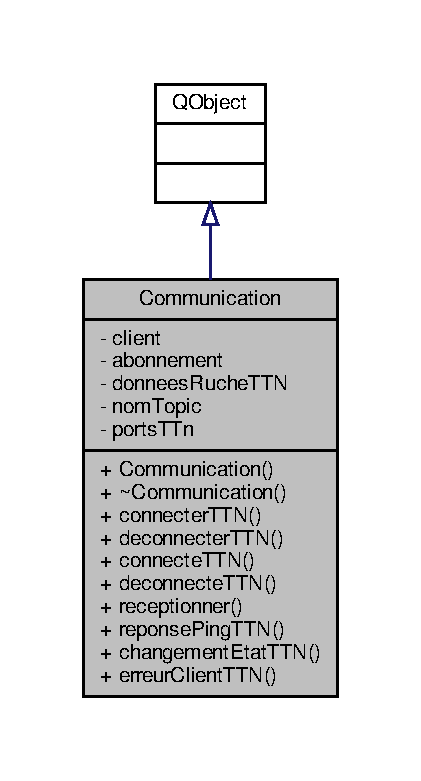
\includegraphics[width=202pt]{class_communication__coll__graph}
\end{center}
\end{figure}
\subsubsection*{Connecteurs publics}
\begin{DoxyCompactItemize}
\item 
void \hyperlink{class_communication_af71587fb1ee9b7460345b7c12372a1eb}{connecte\+T\+TN} ()
\begin{DoxyCompactList}\small\item\em slot permetant la connection au serveur ttn \end{DoxyCompactList}\item 
void \hyperlink{class_communication_ab0f5a47c2fc7dbca198bfab2c0ac65bb}{deconnecte\+T\+TN} ()
\begin{DoxyCompactList}\small\item\em slot permetant la deconnection au serveur ttn \end{DoxyCompactList}\item 
void \hyperlink{class_communication_a9a0c0ce96c86cbb3e59529b2334819f3}{receptionner} (const Q\+Byte\+Array \&message, const Q\+Mqtt\+Topic\+Name \&topic)
\begin{DoxyCompactList}\small\item\em slot permetant la reception des donnée grace au protocole mqtt \end{DoxyCompactList}\item 
void \hyperlink{class_communication_a2921a3a80cdcb10f7f63c3bd779d7129}{reponse\+Ping\+T\+TN} ()
\begin{DoxyCompactList}\small\item\em slot permetant d\textquotesingle{}effectuer un ping vers le serveur ttn \end{DoxyCompactList}\item 
void \hyperlink{class_communication_af249c498d61b4288b9e7d388baf81fc2}{changement\+Etat\+T\+TN} ()
\begin{DoxyCompactList}\small\item\em slot permetant de recevoir l\textquotesingle{}etat du serveur ttn \end{DoxyCompactList}\item 
void \hyperlink{class_communication_ae1a84ffd9317d0e4e27a6633cef43b64}{erreur\+Client\+T\+TN} ()
\begin{DoxyCompactList}\small\item\em slot permetant de recevoir les erreur rencontré lors de la connection au serveur ttn \end{DoxyCompactList}\end{DoxyCompactItemize}
\subsubsection*{Signaux}
\begin{DoxyCompactItemize}
\item 
void \hyperlink{class_communication_aa6100d6b2addece57f3e74c1140a3179}{etat\+Client\+Connexion} (bool connexion)
\item 
void \hyperlink{class_communication_a83865ed4092e263f42669dff0582b7e1}{message\+Recu} (const Q\+Byte\+Array \&message, const Q\+Mqtt\+Topic\+Name \&topic)
\end{DoxyCompactItemize}
\subsubsection*{Fonctions membres publiques}
\begin{DoxyCompactItemize}
\item 
\hyperlink{class_communication_a7376830f5598b7e3c0eb4434a8a8766e}{Communication} (Q\+String\+List \hyperlink{class_communication_a5b7ff98c422c16085e7dc422f2ae51c5}{donnees\+Ruche\+T\+TN}, \hyperlink{class_q_object}{Q\+Object} $\ast$parent=0)
\begin{DoxyCompactList}\small\item\em Constructeur de la classe \hyperlink{class_communication}{Communication}. \end{DoxyCompactList}\item 
\hyperlink{class_communication_a75ba08ce908d45251e28e4c1db94e6f4}{$\sim$\+Communication} ()
\begin{DoxyCompactList}\small\item\em destructeur de la classse \hyperlink{class_communication}{Communication} \end{DoxyCompactList}\item 
void \hyperlink{class_communication_aadec726c44e719fa587bd385533eb559}{connecter\+T\+TN} ()
\item 
void \hyperlink{class_communication_a8d0cc5c992a2b218a64f57429eea001b}{deconnecter\+T\+TN} ()
\end{DoxyCompactItemize}
\subsubsection*{Attributs privés}
\begin{DoxyCompactItemize}
\item 
Q\+Mqtt\+Client $\ast$ \hyperlink{class_communication_a59ae01a54d6c3fde6242c46d802b954b}{client}
\item 
Q\+Mqtt\+Subscription $\ast$ \hyperlink{class_communication_af29011664fbb15b9fb41ce37b70a694f}{abonnement}
\item 
Q\+String\+List \hyperlink{class_communication_a5b7ff98c422c16085e7dc422f2ae51c5}{donnees\+Ruche\+T\+TN}
\item 
Q\+String \hyperlink{class_communication_a7d536b64ee7a5373047c292477d391d5}{nom\+Topic}
\item 
\hyperlink{parametres_8h_a0fe68caa1e9147addc96657cc822b937}{Ports\+T\+TN} \hyperlink{class_communication_aba7a5df723bc632b957b4358bef8605e}{ports\+T\+Tn}
\end{DoxyCompactItemize}


\subsubsection{Description détaillée}
\begin{DoxyAuthor}{Auteur}
Florentin Mellah, Enzo Rossi
\end{DoxyAuthor}
\begin{DoxyVersion}{Version}
1.\+1 
\end{DoxyVersion}


\subsubsection{Documentation des constructeurs et destructeur}
\mbox{\Hypertarget{class_communication_a7376830f5598b7e3c0eb4434a8a8766e}\label{class_communication_a7376830f5598b7e3c0eb4434a8a8766e}} 
\index{Communication@{Communication}!Communication@{Communication}}
\index{Communication@{Communication}!Communication@{Communication}}
\paragraph{\texorpdfstring{Communication()}{Communication()}}
{\footnotesize\ttfamily Communication\+::\+Communication (\begin{DoxyParamCaption}\item[{Q\+String\+List}]{donnees\+Ruche\+T\+TN,  }\item[{\hyperlink{class_q_object}{Q\+Object} $\ast$}]{parent = {\ttfamily 0} }\end{DoxyParamCaption})}


\begin{DoxyParams}{Paramètres}
{\em parent} & \hyperlink{class_q_object}{Q\+Object} Adresse de l\textquotesingle{}objet Qt parent (0 = fenêtre principale)\\
\hline
\end{DoxyParams}
Définition des attributs client , abonement et nom\+Topic a 0 (=null) 

Références \hyperlink{class_communication_af249c498d61b4288b9e7d388baf81fc2}{changement\+Etat\+T\+T\+N()}, \hyperlink{class_communication_a59ae01a54d6c3fde6242c46d802b954b}{client}, \hyperlink{class_communication_aadec726c44e719fa587bd385533eb559}{connecter\+T\+T\+N()}, \hyperlink{class_communication_af71587fb1ee9b7460345b7c12372a1eb}{connecte\+T\+T\+N()}, \hyperlink{class_communication_ab0f5a47c2fc7dbca198bfab2c0ac65bb}{deconnecte\+T\+T\+N()}, \hyperlink{class_communication_ae1a84ffd9317d0e4e27a6633cef43b64}{erreur\+Client\+T\+T\+N()}, \hyperlink{class_communication_a7d536b64ee7a5373047c292477d391d5}{nom\+Topic}, \hyperlink{class_communication_a9a0c0ce96c86cbb3e59529b2334819f3}{receptionner()}, et \hyperlink{class_communication_a2921a3a80cdcb10f7f63c3bd779d7129}{reponse\+Ping\+T\+T\+N()}.


\begin{DoxyCode}
00027                                                                          : 
      \hyperlink{class_q_object}{QObject}(parent), \hyperlink{class_communication_a59ae01a54d6c3fde6242c46d802b954b}{client}(0), \hyperlink{class_communication_af29011664fbb15b9fb41ce37b70a694f}{abonnement}(0), 
      \hyperlink{class_communication_a5b7ff98c422c16085e7dc422f2ae51c5}{donneesRucheTTN}(\hyperlink{class_communication_a5b7ff98c422c16085e7dc422f2ae51c5}{donneesRucheTTN})
00028 \{
00029     \hyperlink{class_communication_a7d536b64ee7a5373047c292477d391d5}{nomTopic} = \hyperlink{class_communication_a5b7ff98c422c16085e7dc422f2ae51c5}{donneesRucheTTN}.at(6) + \textcolor{stringliteral}{"/devices/"} + 
      \hyperlink{class_communication_a5b7ff98c422c16085e7dc422f2ae51c5}{donneesRucheTTN}.at(2) + \textcolor{stringliteral}{"/up"};
00030     qDebug()<< Q\_FUNC\_INFO << \textcolor{stringliteral}{"donneesRucheTTN"} << \hyperlink{class_communication_a5b7ff98c422c16085e7dc422f2ae51c5}{donneesRucheTTN}  << \textcolor{stringliteral}{"nomTopic"} << 
      \hyperlink{class_communication_a7d536b64ee7a5373047c292477d391d5}{nomTopic};
00031     \hyperlink{class_communication_a59ae01a54d6c3fde6242c46d802b954b}{client} = \textcolor{keyword}{new} QMqttClient();    
00032     connect(\hyperlink{class_communication_a59ae01a54d6c3fde6242c46d802b954b}{client}, SIGNAL(stateChanged(ClientState)), \textcolor{keyword}{this}, SLOT(
      \hyperlink{class_communication_af249c498d61b4288b9e7d388baf81fc2}{changementEtatTTN}()));
00033     connect(\hyperlink{class_communication_a59ae01a54d6c3fde6242c46d802b954b}{client}, SIGNAL(errorChanged(ClientError)), \textcolor{keyword}{this}, SLOT(
      \hyperlink{class_communication_ae1a84ffd9317d0e4e27a6633cef43b64}{erreurClientTTN}()));
00034     connect(\hyperlink{class_communication_a59ae01a54d6c3fde6242c46d802b954b}{client}, SIGNAL(connected()), \textcolor{keyword}{this}, SLOT(\hyperlink{class_communication_af71587fb1ee9b7460345b7c12372a1eb}{connecteTTN}()));
00035     connect(\hyperlink{class_communication_a59ae01a54d6c3fde6242c46d802b954b}{client}, SIGNAL(disconnected()), \textcolor{keyword}{this}, SLOT(\hyperlink{class_communication_ab0f5a47c2fc7dbca198bfab2c0ac65bb}{deconnecteTTN}()));
00036     connect(\hyperlink{class_communication_a59ae01a54d6c3fde6242c46d802b954b}{client}, SIGNAL(messageReceived(\textcolor{keyword}{const} QByteArray &, \textcolor{keyword}{const} QMqttTopicName &)), \textcolor{keyword}{this}, SLOT(
      \hyperlink{class_communication_a9a0c0ce96c86cbb3e59529b2334819f3}{receptionner}(\textcolor{keyword}{const} QByteArray &, \textcolor{keyword}{const} QMqttTopicName &)));
00037     connect(\hyperlink{class_communication_a59ae01a54d6c3fde6242c46d802b954b}{client}, SIGNAL(pingResponseReceived()), \textcolor{keyword}{this}, SLOT(
      \hyperlink{class_communication_a2921a3a80cdcb10f7f63c3bd779d7129}{reponsePingTTN}()));
00038     \hyperlink{class_communication_aadec726c44e719fa587bd385533eb559}{connecterTTN}();
00039 \}
\end{DoxyCode}
\mbox{\Hypertarget{class_communication_a75ba08ce908d45251e28e4c1db94e6f4}\label{class_communication_a75ba08ce908d45251e28e4c1db94e6f4}} 
\index{Communication@{Communication}!````~Communication@{$\sim$\+Communication}}
\index{````~Communication@{$\sim$\+Communication}!Communication@{Communication}}
\paragraph{\texorpdfstring{$\sim$\+Communication()}{~Communication()}}
{\footnotesize\ttfamily Communication\+::$\sim$\+Communication (\begin{DoxyParamCaption}{ }\end{DoxyParamCaption})}



Références \hyperlink{class_communication_af29011664fbb15b9fb41ce37b70a694f}{abonnement}, \hyperlink{class_communication_a59ae01a54d6c3fde6242c46d802b954b}{client}, et \hyperlink{class_communication_a8d0cc5c992a2b218a64f57429eea001b}{deconnecter\+T\+T\+N()}.


\begin{DoxyCode}
00045 \{
00046     \hyperlink{class_communication_a8d0cc5c992a2b218a64f57429eea001b}{deconnecterTTN}();
00047     \textcolor{keyword}{delete} \hyperlink{class_communication_af29011664fbb15b9fb41ce37b70a694f}{abonnement};
00048     \textcolor{keyword}{delete} \hyperlink{class_communication_a59ae01a54d6c3fde6242c46d802b954b}{client};
00049     qDebug() << Q\_FUNC\_INFO;
00050 \}
\end{DoxyCode}


\subsubsection{Documentation des fonctions membres}
\mbox{\Hypertarget{class_communication_af249c498d61b4288b9e7d388baf81fc2}\label{class_communication_af249c498d61b4288b9e7d388baf81fc2}} 
\index{Communication@{Communication}!changement\+Etat\+T\+TN@{changement\+Etat\+T\+TN}}
\index{changement\+Etat\+T\+TN@{changement\+Etat\+T\+TN}!Communication@{Communication}}
\paragraph{\texorpdfstring{changement\+Etat\+T\+TN}{changementEtatTTN}}
{\footnotesize\ttfamily void Communication\+::changement\+Etat\+T\+TN (\begin{DoxyParamCaption}{ }\end{DoxyParamCaption})\hspace{0.3cm}{\ttfamily [slot]}}



Références \hyperlink{class_communication_a59ae01a54d6c3fde6242c46d802b954b}{client}.



Référencé par \hyperlink{class_communication_a7376830f5598b7e3c0eb4434a8a8766e}{Communication()}.


\begin{DoxyCode}
00126 \{
00127     \textcolor{comment}{// Pour le debug}
00128     QString message;
00129     \textcolor{keywordflow}{switch}(\hyperlink{class_communication_a59ae01a54d6c3fde6242c46d802b954b}{client}->state())
00130     \{
00131         \textcolor{keywordflow}{case} 0: message = \textcolor{stringliteral}{"Déconnecté"}; \textcolor{keywordflow}{break};
00132         \textcolor{keywordflow}{case} 1: message = \textcolor{stringliteral}{"En cours de connexion"}; \textcolor{keywordflow}{break};
00133         \textcolor{keywordflow}{case} 2: message = \textcolor{stringliteral}{"Connecté"}; \textcolor{keywordflow}{break};
00134     \}
00135     qDebug()<< Q\_FUNC\_INFO << \textcolor{stringliteral}{"client MQTT"} << message << \textcolor{stringliteral}{"state="} << \hyperlink{class_communication_a59ae01a54d6c3fde6242c46d802b954b}{client}->state();
00136 \}
\end{DoxyCode}
\mbox{\Hypertarget{class_communication_aadec726c44e719fa587bd385533eb559}\label{class_communication_aadec726c44e719fa587bd385533eb559}} 
\index{Communication@{Communication}!connecter\+T\+TN@{connecter\+T\+TN}}
\index{connecter\+T\+TN@{connecter\+T\+TN}!Communication@{Communication}}
\paragraph{\texorpdfstring{connecter\+T\+T\+N()}{connecterTTN()}}
{\footnotesize\ttfamily void Communication\+::connecter\+T\+TN (\begin{DoxyParamCaption}{ }\end{DoxyParamCaption})}



Références \hyperlink{class_communication_a59ae01a54d6c3fde6242c46d802b954b}{client}, et \hyperlink{class_communication_a5b7ff98c422c16085e7dc422f2ae51c5}{donnees\+Ruche\+T\+TN}.



Référencé par \hyperlink{class_communication_a7376830f5598b7e3c0eb4434a8a8766e}{Communication()}.


\begin{DoxyCode}
00053 \{
00054     qDebug()<< Q\_FUNC\_INFO << \hyperlink{class_communication_a5b7ff98c422c16085e7dc422f2ae51c5}{donneesRucheTTN}.at(4) << 
      \hyperlink{class_communication_a5b7ff98c422c16085e7dc422f2ae51c5}{donneesRucheTTN}.at(5).toInt()  << \hyperlink{class_communication_a5b7ff98c422c16085e7dc422f2ae51c5}{donneesRucheTTN}.at(6) << 
      \hyperlink{class_communication_a5b7ff98c422c16085e7dc422f2ae51c5}{donneesRucheTTN}.at(7);
00055     \hyperlink{class_communication_a59ae01a54d6c3fde6242c46d802b954b}{client}->setHostname(\hyperlink{class_communication_a5b7ff98c422c16085e7dc422f2ae51c5}{donneesRucheTTN}.at(4));
00056     \hyperlink{class_communication_a59ae01a54d6c3fde6242c46d802b954b}{client}->setPort(\hyperlink{class_communication_a5b7ff98c422c16085e7dc422f2ae51c5}{donneesRucheTTN}.at(5).toInt());
00057     \hyperlink{class_communication_a59ae01a54d6c3fde6242c46d802b954b}{client}->setUsername(\hyperlink{class_communication_a5b7ff98c422c16085e7dc422f2ae51c5}{donneesRucheTTN}.at(6));
00058     \hyperlink{class_communication_a59ae01a54d6c3fde6242c46d802b954b}{client}->setPassword(\hyperlink{class_communication_a5b7ff98c422c16085e7dc422f2ae51c5}{donneesRucheTTN}.at(7));
00059     \hyperlink{class_communication_a59ae01a54d6c3fde6242c46d802b954b}{client}->connectToHost();
00060 \}
\end{DoxyCode}
\mbox{\Hypertarget{class_communication_af71587fb1ee9b7460345b7c12372a1eb}\label{class_communication_af71587fb1ee9b7460345b7c12372a1eb}} 
\index{Communication@{Communication}!connecte\+T\+TN@{connecte\+T\+TN}}
\index{connecte\+T\+TN@{connecte\+T\+TN}!Communication@{Communication}}
\paragraph{\texorpdfstring{connecte\+T\+TN}{connecteTTN}}
{\footnotesize\ttfamily void Communication\+::connecte\+T\+TN (\begin{DoxyParamCaption}{ }\end{DoxyParamCaption})\hspace{0.3cm}{\ttfamily [slot]}}



Références \hyperlink{class_communication_af29011664fbb15b9fb41ce37b70a694f}{abonnement}, \hyperlink{parametres_8h_ace364d1ce44aa9f79bcff6e3752c4a5f}{A\+P\+P\+\_\+\+T\+I\+T\+RE}, \hyperlink{class_communication_a59ae01a54d6c3fde6242c46d802b954b}{client}, \hyperlink{class_communication_aa6100d6b2addece57f3e74c1140a3179}{etat\+Client\+Connexion()}, et \hyperlink{class_communication_a7d536b64ee7a5373047c292477d391d5}{nom\+Topic}.



Référencé par \hyperlink{class_communication_a7376830f5598b7e3c0eb4434a8a8766e}{Communication()}.


\begin{DoxyCode}
00072 \{
00073     qDebug() << Q\_FUNC\_INFO << \hyperlink{class_communication_a7d536b64ee7a5373047c292477d391d5}{nomTopic};
00074     \textcolor{comment}{// Le client est maintenant connecté}
00075     emit \hyperlink{class_communication_aa6100d6b2addece57f3e74c1140a3179}{etatClientConnexion}(\textcolor{keyword}{true}); \textcolor{comment}{// pour l'IHM}
00076     \textcolor{comment}{// Souscription à un topic :}
00077     \hyperlink{class_communication_af29011664fbb15b9fb41ce37b70a694f}{abonnement} = \hyperlink{class_communication_a59ae01a54d6c3fde6242c46d802b954b}{client}->subscribe(nomTopic);
00078     \textcolor{keywordflow}{if} (!\hyperlink{class_communication_af29011664fbb15b9fb41ce37b70a694f}{abonnement})
00079     \{
00080         qDebug() << Q\_FUNC\_INFO << \textcolor{stringliteral}{"Impossible de s'abonner au broker TTN !"};
00081         QMessageBox::critical(0, QString::fromUtf8(\hyperlink{parametres_8h_ace364d1ce44aa9f79bcff6e3752c4a5f}{APP\_TITRE}), QString::fromUtf8(\textcolor{stringliteral}{"Impossible de
       s'abonner au broker The Things Network!"}));
00082     \}
00083 \}
\end{DoxyCode}
\mbox{\Hypertarget{class_communication_a8d0cc5c992a2b218a64f57429eea001b}\label{class_communication_a8d0cc5c992a2b218a64f57429eea001b}} 
\index{Communication@{Communication}!deconnecter\+T\+TN@{deconnecter\+T\+TN}}
\index{deconnecter\+T\+TN@{deconnecter\+T\+TN}!Communication@{Communication}}
\paragraph{\texorpdfstring{deconnecter\+T\+T\+N()}{deconnecterTTN()}}
{\footnotesize\ttfamily void Communication\+::deconnecter\+T\+TN (\begin{DoxyParamCaption}{ }\end{DoxyParamCaption})}



Références \hyperlink{class_communication_a59ae01a54d6c3fde6242c46d802b954b}{client}.



Référencé par \hyperlink{class_communication_a75ba08ce908d45251e28e4c1db94e6f4}{$\sim$\+Communication()}.


\begin{DoxyCode}
00063 \{
00064     \hyperlink{class_communication_a59ae01a54d6c3fde6242c46d802b954b}{client}->disconnectFromHost();
00065 \}
\end{DoxyCode}
\mbox{\Hypertarget{class_communication_ab0f5a47c2fc7dbca198bfab2c0ac65bb}\label{class_communication_ab0f5a47c2fc7dbca198bfab2c0ac65bb}} 
\index{Communication@{Communication}!deconnecte\+T\+TN@{deconnecte\+T\+TN}}
\index{deconnecte\+T\+TN@{deconnecte\+T\+TN}!Communication@{Communication}}
\paragraph{\texorpdfstring{deconnecte\+T\+TN}{deconnecteTTN}}
{\footnotesize\ttfamily void Communication\+::deconnecte\+T\+TN (\begin{DoxyParamCaption}{ }\end{DoxyParamCaption})\hspace{0.3cm}{\ttfamily [slot]}}



Références \hyperlink{class_communication_aa6100d6b2addece57f3e74c1140a3179}{etat\+Client\+Connexion()}.



Référencé par \hyperlink{class_communication_a7376830f5598b7e3c0eb4434a8a8766e}{Communication()}.


\begin{DoxyCode}
00090 \{
00091     qDebug()<< Q\_FUNC\_INFO;
00092     \textcolor{comment}{// Le client est maintenant déconnecté}
00093     emit \hyperlink{class_communication_aa6100d6b2addece57f3e74c1140a3179}{etatClientConnexion}(\textcolor{keyword}{false}); \textcolor{comment}{// pour l'IHM}
00094 \}
\end{DoxyCode}
\mbox{\Hypertarget{class_communication_ae1a84ffd9317d0e4e27a6633cef43b64}\label{class_communication_ae1a84ffd9317d0e4e27a6633cef43b64}} 
\index{Communication@{Communication}!erreur\+Client\+T\+TN@{erreur\+Client\+T\+TN}}
\index{erreur\+Client\+T\+TN@{erreur\+Client\+T\+TN}!Communication@{Communication}}
\paragraph{\texorpdfstring{erreur\+Client\+T\+TN}{erreurClientTTN}}
{\footnotesize\ttfamily void Communication\+::erreur\+Client\+T\+TN (\begin{DoxyParamCaption}{ }\end{DoxyParamCaption})\hspace{0.3cm}{\ttfamily [slot]}}

\begin{DoxyRefDesc}{A faire}
\item[\hyperlink{todo__todo000005}{A faire}]Faire une boîte de dialogue d\textquotesingle{}information sur l\textquotesingle{}erreur rencontrée \end{DoxyRefDesc}


Références \hyperlink{class_communication_a59ae01a54d6c3fde6242c46d802b954b}{client}.



Référencé par \hyperlink{class_communication_a7376830f5598b7e3c0eb4434a8a8766e}{Communication()}.


\begin{DoxyCode}
00144 \{
00145 
00146         \textcolor{comment}{/*QMqttClient::NoError                0 No error occurred.}
00147 \textcolor{comment}{        QMqttClient::InvalidProtocolVersion 1   The broker does not accept a connection using the specified
       protocol version.}
00148 \textcolor{comment}{        QMqttClient::IdRejected             2   The client ID is malformed. This might be related to its
       length.}
00149 \textcolor{comment}{        QMqttClient::ServerUnavailable      3   The network connection has been established, but the
       service is unavailable on the broker side.}
00150 \textcolor{comment}{        QMqttClient::BadUsernameOrPassword  4   The data in the username or password is malformed.}
00151 \textcolor{comment}{        QMqttClient::NotAuthorized          5   The client is not authorized to connect.}
00152 \textcolor{comment}{        QMqttClient::TransportInvalid       256 The underlying transport caused an error. For example, the
       connection might have been interrupted unexpectedly.}
00153 \textcolor{comment}{        QMqttClient::ProtocolViolation      257 The client encountered a protocol violation, and therefore
       closed the connection.}
00154 \textcolor{comment}{        QMqttClient::UnknownError           258 An unknown error occurred.}
00155 \textcolor{comment}{        QMqttClient::Mqtt5SpecificError     259 The error is related to MQTT protocol level 5. A reason
       code might provide more details.*/}
00156 
00160     qDebug()<< Q\_FUNC\_INFO << \textcolor{stringliteral}{"code erreur"} << \hyperlink{class_communication_a59ae01a54d6c3fde6242c46d802b954b}{client}->error();
00161 \}
\end{DoxyCode}
\mbox{\Hypertarget{class_communication_aa6100d6b2addece57f3e74c1140a3179}\label{class_communication_aa6100d6b2addece57f3e74c1140a3179}} 
\index{Communication@{Communication}!etat\+Client\+Connexion@{etat\+Client\+Connexion}}
\index{etat\+Client\+Connexion@{etat\+Client\+Connexion}!Communication@{Communication}}
\paragraph{\texorpdfstring{etat\+Client\+Connexion}{etatClientConnexion}}
{\footnotesize\ttfamily void Communication\+::etat\+Client\+Connexion (\begin{DoxyParamCaption}\item[{bool}]{connexion }\end{DoxyParamCaption})\hspace{0.3cm}{\ttfamily [signal]}}



Référencé par \hyperlink{class_communication_af71587fb1ee9b7460345b7c12372a1eb}{connecte\+T\+T\+N()}, et \hyperlink{class_communication_ab0f5a47c2fc7dbca198bfab2c0ac65bb}{deconnecte\+T\+T\+N()}.

\mbox{\Hypertarget{class_communication_a83865ed4092e263f42669dff0582b7e1}\label{class_communication_a83865ed4092e263f42669dff0582b7e1}} 
\index{Communication@{Communication}!message\+Recu@{message\+Recu}}
\index{message\+Recu@{message\+Recu}!Communication@{Communication}}
\paragraph{\texorpdfstring{message\+Recu}{messageRecu}}
{\footnotesize\ttfamily void Communication\+::message\+Recu (\begin{DoxyParamCaption}\item[{const Q\+Byte\+Array \&}]{message,  }\item[{const Q\+Mqtt\+Topic\+Name \&}]{topic }\end{DoxyParamCaption})\hspace{0.3cm}{\ttfamily [signal]}}



Référencé par \hyperlink{class_communication_a9a0c0ce96c86cbb3e59529b2334819f3}{receptionner()}.

\mbox{\Hypertarget{class_communication_a9a0c0ce96c86cbb3e59529b2334819f3}\label{class_communication_a9a0c0ce96c86cbb3e59529b2334819f3}} 
\index{Communication@{Communication}!receptionner@{receptionner}}
\index{receptionner@{receptionner}!Communication@{Communication}}
\paragraph{\texorpdfstring{receptionner}{receptionner}}
{\footnotesize\ttfamily void Communication\+::receptionner (\begin{DoxyParamCaption}\item[{const Q\+Byte\+Array \&}]{message,  }\item[{const Q\+Mqtt\+Topic\+Name \&}]{topic }\end{DoxyParamCaption})\hspace{0.3cm}{\ttfamily [slot]}}


\begin{DoxyParams}{Paramètres}
{\em message} & correspondant au données recu \\
\hline
{\em topic} & correspondant au nom de topic \\
\hline
\end{DoxyParams}


Références \hyperlink{class_communication_a83865ed4092e263f42669dff0582b7e1}{message\+Recu()}.



Référencé par \hyperlink{class_communication_a7376830f5598b7e3c0eb4434a8a8766e}{Communication()}.


\begin{DoxyCode}
00104 \{
00105     \textcolor{comment}{//qDebug() << Q\_FUNC\_INFO << topic;}
00106     emit \hyperlink{class_communication_a83865ed4092e263f42669dff0582b7e1}{messageRecu}(message, topic);
00107 \}
\end{DoxyCode}
\mbox{\Hypertarget{class_communication_a2921a3a80cdcb10f7f63c3bd779d7129}\label{class_communication_a2921a3a80cdcb10f7f63c3bd779d7129}} 
\index{Communication@{Communication}!reponse\+Ping\+T\+TN@{reponse\+Ping\+T\+TN}}
\index{reponse\+Ping\+T\+TN@{reponse\+Ping\+T\+TN}!Communication@{Communication}}
\paragraph{\texorpdfstring{reponse\+Ping\+T\+TN}{reponsePingTTN}}
{\footnotesize\ttfamily void Communication\+::reponse\+Ping\+T\+TN (\begin{DoxyParamCaption}{ }\end{DoxyParamCaption})\hspace{0.3cm}{\ttfamily [slot]}}



Référencé par \hyperlink{class_communication_a7376830f5598b7e3c0eb4434a8a8766e}{Communication()}.


\begin{DoxyCode}
00115 \{
00116     \textcolor{comment}{// Pour les tests (requestPing())}
00117     qDebug()<< Q\_FUNC\_INFO;
00118 \}
\end{DoxyCode}


\subsubsection{Documentation des données membres}
\mbox{\Hypertarget{class_communication_af29011664fbb15b9fb41ce37b70a694f}\label{class_communication_af29011664fbb15b9fb41ce37b70a694f}} 
\index{Communication@{Communication}!abonnement@{abonnement}}
\index{abonnement@{abonnement}!Communication@{Communication}}
\paragraph{\texorpdfstring{abonnement}{abonnement}}
{\footnotesize\ttfamily Q\+Mqtt\+Subscription$\ast$ Communication\+::abonnement\hspace{0.3cm}{\ttfamily [private]}}



Référencé par \hyperlink{class_communication_af71587fb1ee9b7460345b7c12372a1eb}{connecte\+T\+T\+N()}, et \hyperlink{class_communication_a75ba08ce908d45251e28e4c1db94e6f4}{$\sim$\+Communication()}.

\mbox{\Hypertarget{class_communication_a59ae01a54d6c3fde6242c46d802b954b}\label{class_communication_a59ae01a54d6c3fde6242c46d802b954b}} 
\index{Communication@{Communication}!client@{client}}
\index{client@{client}!Communication@{Communication}}
\paragraph{\texorpdfstring{client}{client}}
{\footnotesize\ttfamily Q\+Mqtt\+Client$\ast$ Communication\+::client\hspace{0.3cm}{\ttfamily [private]}}



Référencé par \hyperlink{class_communication_af249c498d61b4288b9e7d388baf81fc2}{changement\+Etat\+T\+T\+N()}, \hyperlink{class_communication_a7376830f5598b7e3c0eb4434a8a8766e}{Communication()}, \hyperlink{class_communication_aadec726c44e719fa587bd385533eb559}{connecter\+T\+T\+N()}, \hyperlink{class_communication_af71587fb1ee9b7460345b7c12372a1eb}{connecte\+T\+T\+N()}, \hyperlink{class_communication_a8d0cc5c992a2b218a64f57429eea001b}{deconnecter\+T\+T\+N()}, \hyperlink{class_communication_ae1a84ffd9317d0e4e27a6633cef43b64}{erreur\+Client\+T\+T\+N()}, et \hyperlink{class_communication_a75ba08ce908d45251e28e4c1db94e6f4}{$\sim$\+Communication()}.

\mbox{\Hypertarget{class_communication_a5b7ff98c422c16085e7dc422f2ae51c5}\label{class_communication_a5b7ff98c422c16085e7dc422f2ae51c5}} 
\index{Communication@{Communication}!donnees\+Ruche\+T\+TN@{donnees\+Ruche\+T\+TN}}
\index{donnees\+Ruche\+T\+TN@{donnees\+Ruche\+T\+TN}!Communication@{Communication}}
\paragraph{\texorpdfstring{donnees\+Ruche\+T\+TN}{donneesRucheTTN}}
{\footnotesize\ttfamily Q\+String\+List Communication\+::donnees\+Ruche\+T\+TN\hspace{0.3cm}{\ttfamily [private]}}



Référencé par \hyperlink{class_communication_aadec726c44e719fa587bd385533eb559}{connecter\+T\+T\+N()}.

\mbox{\Hypertarget{class_communication_a7d536b64ee7a5373047c292477d391d5}\label{class_communication_a7d536b64ee7a5373047c292477d391d5}} 
\index{Communication@{Communication}!nom\+Topic@{nom\+Topic}}
\index{nom\+Topic@{nom\+Topic}!Communication@{Communication}}
\paragraph{\texorpdfstring{nom\+Topic}{nomTopic}}
{\footnotesize\ttfamily Q\+String Communication\+::nom\+Topic\hspace{0.3cm}{\ttfamily [private]}}



Référencé par \hyperlink{class_communication_a7376830f5598b7e3c0eb4434a8a8766e}{Communication()}, et \hyperlink{class_communication_af71587fb1ee9b7460345b7c12372a1eb}{connecte\+T\+T\+N()}.

\mbox{\Hypertarget{class_communication_aba7a5df723bc632b957b4358bef8605e}\label{class_communication_aba7a5df723bc632b957b4358bef8605e}} 
\index{Communication@{Communication}!ports\+T\+Tn@{ports\+T\+Tn}}
\index{ports\+T\+Tn@{ports\+T\+Tn}!Communication@{Communication}}
\paragraph{\texorpdfstring{ports\+T\+Tn}{portsTTn}}
{\footnotesize\ttfamily \hyperlink{parametres_8h_a0fe68caa1e9147addc96657cc822b937}{Ports\+T\+TN} Communication\+::ports\+T\+Tn\hspace{0.3cm}{\ttfamily [private]}}



La documentation de cette classe a été générée à partir des fichiers suivants \+:\begin{DoxyCompactItemize}
\item 
\hyperlink{communication_8h}{communication.\+h}\item 
\hyperlink{communication_8cpp}{communication.\+cpp}\end{DoxyCompactItemize}

\hypertarget{classfr_1_1campus_1_1laurainc_1_1honeybee_1_1_base_de_donnees_1_1_connexion_my_sql}{}\subsection{Référence de la classe fr.\+campus.\+laurainc.\+honeybee.\+Base\+De\+Donnees.\+Connexion\+My\+Sql}
\label{classfr_1_1campus_1_1laurainc_1_1honeybee_1_1_base_de_donnees_1_1_connexion_my_sql}\index{fr.\+campus.\+laurainc.\+honeybee.\+Base\+De\+Donnees.\+Connexion\+My\+Sql@{fr.\+campus.\+laurainc.\+honeybee.\+Base\+De\+Donnees.\+Connexion\+My\+Sql}}


Classe permettant de se connecter à My\+S\+QL en arrière-\/plan.  




Graphe de collaboration de fr.\+campus.\+laurainc.\+honeybee.\+Base\+De\+Donnees.\+Connexion\+My\+Sql\+:\nopagebreak
\begin{figure}[H]
\begin{center}
\leavevmode
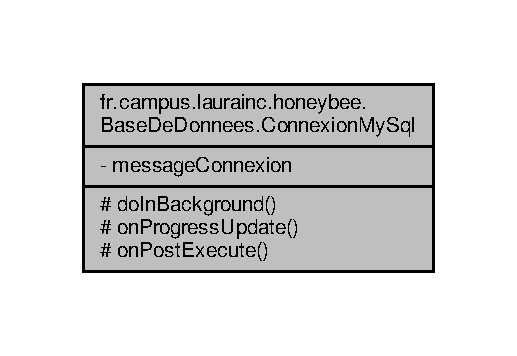
\includegraphics[width=248pt]{classfr_1_1campus_1_1laurainc_1_1honeybee_1_1_base_de_donnees_1_1_connexion_my_sql__coll__graph}
\end{center}
\end{figure}
\subsubsection*{Fonctions membres protégées}
\begin{DoxyCompactItemize}
\item 
Boolean \hyperlink{classfr_1_1campus_1_1laurainc_1_1honeybee_1_1_base_de_donnees_1_1_connexion_my_sql_a752c9f0f9a0879fceeeabd48c5fcb058}{do\+In\+Background} (Void... unused)
\begin{DoxyCompactList}\small\item\em Méthode de connexion qui s’exécute dans un autre thread. \end{DoxyCompactList}\item 
void \hyperlink{classfr_1_1campus_1_1laurainc_1_1honeybee_1_1_base_de_donnees_1_1_connexion_my_sql_ab9c34193cf45af727a5f5de4b27b1a46}{on\+Progress\+Update} (Integer... progress)
\begin{DoxyCompactList}\small\item\em Méthode permettant d\textquotesingle{}indiquer la progression de la tâche d\textquotesingle{}arrière plan (s’exécute dans le thread UI) \end{DoxyCompactList}\item 
void \hyperlink{classfr_1_1campus_1_1laurainc_1_1honeybee_1_1_base_de_donnees_1_1_connexion_my_sql_acea6398eed8fc31f2a847f1e4452046c}{on\+Post\+Execute} (Boolean result)
\end{DoxyCompactItemize}
\subsubsection*{Attributs privés}
\begin{DoxyCompactItemize}
\item 
String \hyperlink{classfr_1_1campus_1_1laurainc_1_1honeybee_1_1_base_de_donnees_1_1_connexion_my_sql_a8db83810efa310195fdd72bcbac2843f}{message\+Connexion} = \char`\"{}\char`\"{}
\end{DoxyCompactItemize}


\subsubsection{Documentation des fonctions membres}
\mbox{\Hypertarget{classfr_1_1campus_1_1laurainc_1_1honeybee_1_1_base_de_donnees_1_1_connexion_my_sql_a752c9f0f9a0879fceeeabd48c5fcb058}\label{classfr_1_1campus_1_1laurainc_1_1honeybee_1_1_base_de_donnees_1_1_connexion_my_sql_a752c9f0f9a0879fceeeabd48c5fcb058}} 
\index{fr\+::campus\+::laurainc\+::honeybee\+::\+Base\+De\+Donnees\+::\+Connexion\+My\+Sql@{fr\+::campus\+::laurainc\+::honeybee\+::\+Base\+De\+Donnees\+::\+Connexion\+My\+Sql}!do\+In\+Background@{do\+In\+Background}}
\index{do\+In\+Background@{do\+In\+Background}!fr\+::campus\+::laurainc\+::honeybee\+::\+Base\+De\+Donnees\+::\+Connexion\+My\+Sql@{fr\+::campus\+::laurainc\+::honeybee\+::\+Base\+De\+Donnees\+::\+Connexion\+My\+Sql}}
\paragraph{\texorpdfstring{do\+In\+Background()}{doInBackground()}}
{\footnotesize\ttfamily fr.\+campus.\+laurainc.\+honeybee.\+Base\+De\+Donnees.\+Connexion\+My\+Sql.\+do\+In\+Background (\begin{DoxyParamCaption}\item[{Void...}]{unused }\end{DoxyParamCaption})\hspace{0.3cm}{\ttfamily [protected]}}



Références \hyperlink{classfr_1_1campus_1_1laurainc_1_1honeybee_1_1_base_de_donnees_a735f54c2c183a595c9a9a5ba947491f5}{fr.\+campus.\+laurainc.\+honeybee.\+Base\+De\+Donnees.\+est\+Connecte()}.


\begin{DoxyCode}
00300         \{
00301             \textcolor{keywordflow}{try}
00302             \{
00303                 \textcolor{comment}{// chargement du pilote JDBC MySQL}
00304                 publishProgress(1);
00305                 Class.forName(\textcolor{stringliteral}{"com.mysql.jdbc.Driver"}).newInstance();
00306             \}
00307             \textcolor{keywordflow}{catch} (Exception e)
00308             \{
00309                 e.printStackTrace();
00310                 Log.e(\hyperlink{classfr_1_1campus_1_1laurainc_1_1honeybee_1_1_base_de_donnees_ae800d867b3e423dd139e982736ab5587}{TAG}, \textcolor{stringliteral}{"doInBackground -> exception : "} + e.toString());
00311                 \hyperlink{classfr_1_1campus_1_1laurainc_1_1honeybee_1_1_base_de_donnees_1_1_connexion_my_sql_a8db83810efa310195fdd72bcbac2843f}{messageConnexion} = \textcolor{stringliteral}{"Erreur connexion MySQL !"};
00312             \}
00313             \textcolor{keywordflow}{try}
00314             \{
00315                 publishProgress(50);
00316                 \textcolor{keywordflow}{if} (!\hyperlink{classfr_1_1campus_1_1laurainc_1_1honeybee_1_1_base_de_donnees_a735f54c2c183a595c9a9a5ba947491f5}{estConnecte}())
00317                 \{
00318                     \hyperlink{classfr_1_1campus_1_1laurainc_1_1honeybee_1_1_base_de_donnees_a358899633f17b8cd00dd2c4cfdd40abe}{connexion} = DriverManager.getConnection(\hyperlink{classfr_1_1campus_1_1laurainc_1_1honeybee_1_1_base_de_donnees_ad1d04b4da375002e91d8370b9d19918e}{url}, 
      \hyperlink{classfr_1_1campus_1_1laurainc_1_1honeybee_1_1_base_de_donnees_a7d1662e10f11f740155774b625ed1a87}{username}, \hyperlink{classfr_1_1campus_1_1laurainc_1_1honeybee_1_1_base_de_donnees_af1bb604a666a7eee9edd93b6cafaf064}{password});
00319                 \}
00320                 publishProgress(75);
00321                 Log.d(\hyperlink{classfr_1_1campus_1_1laurainc_1_1honeybee_1_1_base_de_donnees_ae800d867b3e423dd139e982736ab5587}{TAG}, \textcolor{stringliteral}{"doInBackground -> connecte : "} + !\hyperlink{classfr_1_1campus_1_1laurainc_1_1honeybee_1_1_base_de_donnees_a358899633f17b8cd00dd2c4cfdd40abe}{connexion}.isClosed());
00322                 \textcolor{keywordflow}{if}(!\hyperlink{classfr_1_1campus_1_1laurainc_1_1honeybee_1_1_base_de_donnees_a358899633f17b8cd00dd2c4cfdd40abe}{connexion}.isClosed())
00323                     \hyperlink{classfr_1_1campus_1_1laurainc_1_1honeybee_1_1_base_de_donnees_1_1_connexion_my_sql_a8db83810efa310195fdd72bcbac2843f}{messageConnexion} = \textcolor{stringliteral}{"Connexion MySQL réussie !"};
00324                 publishProgress(100);
00325                 \textcolor{keywordflow}{return} !\hyperlink{classfr_1_1campus_1_1laurainc_1_1honeybee_1_1_base_de_donnees_a358899633f17b8cd00dd2c4cfdd40abe}{connexion}.isClosed();
00326             \}
00327             \textcolor{keywordflow}{catch} (SQLException e)
00328             \{
00329                 e.printStackTrace();
00330                 Log.e(\hyperlink{classfr_1_1campus_1_1laurainc_1_1honeybee_1_1_base_de_donnees_ae800d867b3e423dd139e982736ab5587}{TAG}, \textcolor{stringliteral}{"doInBackground -> SQLException : "} + e.getMessage());
00331                 Log.e(\hyperlink{classfr_1_1campus_1_1laurainc_1_1honeybee_1_1_base_de_donnees_ae800d867b3e423dd139e982736ab5587}{TAG}, \textcolor{stringliteral}{"doInBackground -> SQLState : "} + e.getSQLState());
00332                 Log.e(\hyperlink{classfr_1_1campus_1_1laurainc_1_1honeybee_1_1_base_de_donnees_ae800d867b3e423dd139e982736ab5587}{TAG}, \textcolor{stringliteral}{"doInBackground -> VendorError : "} + e.getErrorCode());
00333                 \hyperlink{classfr_1_1campus_1_1laurainc_1_1honeybee_1_1_base_de_donnees_1_1_connexion_my_sql_a8db83810efa310195fdd72bcbac2843f}{messageConnexion} = \textcolor{stringliteral}{"Erreur connexion MySQL !"};
00334                 publishProgress(100);
00335                 \textcolor{keywordflow}{return} \textcolor{keyword}{false};
00336             \}
00337         \}
\end{DoxyCode}
\mbox{\Hypertarget{classfr_1_1campus_1_1laurainc_1_1honeybee_1_1_base_de_donnees_1_1_connexion_my_sql_acea6398eed8fc31f2a847f1e4452046c}\label{classfr_1_1campus_1_1laurainc_1_1honeybee_1_1_base_de_donnees_1_1_connexion_my_sql_acea6398eed8fc31f2a847f1e4452046c}} 
\index{fr\+::campus\+::laurainc\+::honeybee\+::\+Base\+De\+Donnees\+::\+Connexion\+My\+Sql@{fr\+::campus\+::laurainc\+::honeybee\+::\+Base\+De\+Donnees\+::\+Connexion\+My\+Sql}!on\+Post\+Execute@{on\+Post\+Execute}}
\index{on\+Post\+Execute@{on\+Post\+Execute}!fr\+::campus\+::laurainc\+::honeybee\+::\+Base\+De\+Donnees\+::\+Connexion\+My\+Sql@{fr\+::campus\+::laurainc\+::honeybee\+::\+Base\+De\+Donnees\+::\+Connexion\+My\+Sql}}
\paragraph{\texorpdfstring{on\+Post\+Execute()}{onPostExecute()}}
{\footnotesize\ttfamily void fr.\+campus.\+laurainc.\+honeybee.\+Base\+De\+Donnees.\+Connexion\+My\+Sql.\+on\+Post\+Execute (\begin{DoxyParamCaption}\item[{Boolean}]{result }\end{DoxyParamCaption})\hspace{0.3cm}{\ttfamily [protected]}}


\begin{DoxyCode}
00362         \{
00363             Log.d(\hyperlink{classfr_1_1campus_1_1laurainc_1_1honeybee_1_1_base_de_donnees_ae800d867b3e423dd139e982736ab5587}{TAG}, \textcolor{stringliteral}{"onPostExecute -> result : "} + result);
00364             Log.d(\hyperlink{classfr_1_1campus_1_1laurainc_1_1honeybee_1_1_base_de_donnees_ae800d867b3e423dd139e982736ab5587}{TAG}, \textcolor{stringliteral}{"onPostExecute -> message : "} + \hyperlink{classfr_1_1campus_1_1laurainc_1_1honeybee_1_1_base_de_donnees_1_1_connexion_my_sql_a8db83810efa310195fdd72bcbac2843f}{messageConnexion});
00365             \textcolor{keywordflow}{if}(result)
00366             \{
00367                 \textcolor{keywordflow}{if}(\hyperlink{classfr_1_1campus_1_1laurainc_1_1honeybee_1_1_base_de_donnees_aad4fd29f29916bc4277fa16262d19431}{activite} != null)
00368                 \{
00369                     \textcolor{comment}{// Ici on peut accéder à la partie UI d'une activité}
00370                     \textcolor{comment}{// et/ou appeler une méthode d'une activité}
00371                 \}
00372             \}
00373             \textcolor{keywordflow}{else}
00374             \{
00375                 \textcolor{keywordflow}{if}(\hyperlink{classfr_1_1campus_1_1laurainc_1_1honeybee_1_1_base_de_donnees_aad4fd29f29916bc4277fa16262d19431}{activite} != null)
00376                 \{
00377                     \textcolor{comment}{// Ici on peut accéder à la partie UI d'une activité}
00378                     \textcolor{comment}{// et/ou appeler une méthode d'une activité}
00379                 \}
00380             \}
00381         \}
\end{DoxyCode}
\mbox{\Hypertarget{classfr_1_1campus_1_1laurainc_1_1honeybee_1_1_base_de_donnees_1_1_connexion_my_sql_ab9c34193cf45af727a5f5de4b27b1a46}\label{classfr_1_1campus_1_1laurainc_1_1honeybee_1_1_base_de_donnees_1_1_connexion_my_sql_ab9c34193cf45af727a5f5de4b27b1a46}} 
\index{fr\+::campus\+::laurainc\+::honeybee\+::\+Base\+De\+Donnees\+::\+Connexion\+My\+Sql@{fr\+::campus\+::laurainc\+::honeybee\+::\+Base\+De\+Donnees\+::\+Connexion\+My\+Sql}!on\+Progress\+Update@{on\+Progress\+Update}}
\index{on\+Progress\+Update@{on\+Progress\+Update}!fr\+::campus\+::laurainc\+::honeybee\+::\+Base\+De\+Donnees\+::\+Connexion\+My\+Sql@{fr\+::campus\+::laurainc\+::honeybee\+::\+Base\+De\+Donnees\+::\+Connexion\+My\+Sql}}
\paragraph{\texorpdfstring{on\+Progress\+Update()}{onProgressUpdate()}}
{\footnotesize\ttfamily fr.\+campus.\+laurainc.\+honeybee.\+Base\+De\+Donnees.\+Connexion\+My\+Sql.\+on\+Progress\+Update (\begin{DoxyParamCaption}\item[{Integer...}]{progress }\end{DoxyParamCaption})\hspace{0.3cm}{\ttfamily [protected]}}

do\+In\+Background peut appeler publish\+Progress() pour indiquer l\textquotesingle{}avancement du traitement ce qui aura pour effet d\textquotesingle{}appeler automatiquement \hyperlink{classfr_1_1campus_1_1laurainc_1_1honeybee_1_1_base_de_donnees_1_1_connexion_my_sql_ab9c34193cf45af727a5f5de4b27b1a46}{on\+Progress\+Update()} 
\begin{DoxyCode}
00346         \{
00347             Log.v(\hyperlink{classfr_1_1campus_1_1laurainc_1_1honeybee_1_1_base_de_donnees_ae800d867b3e423dd139e982736ab5587}{TAG}, \textcolor{stringliteral}{"onProgressUpdate -> progression : "} + progress[0]);
00348             \textcolor{keywordflow}{if}(\hyperlink{classfr_1_1campus_1_1laurainc_1_1honeybee_1_1_base_de_donnees_aad4fd29f29916bc4277fa16262d19431}{activite} != null)
00349             \{
00350                 \textcolor{comment}{// Ici on peut accéder à la partie UI d'une activité}
00351                 \textcolor{comment}{// et/ou appeler une méthode d'une activité}
00352                 \textcolor{comment}{//((MainActivity)activite).afficherProgression(progress[0]);}
00353             \}
00354         \}
\end{DoxyCode}


\subsubsection{Documentation des données membres}
\mbox{\Hypertarget{classfr_1_1campus_1_1laurainc_1_1honeybee_1_1_base_de_donnees_1_1_connexion_my_sql_a8db83810efa310195fdd72bcbac2843f}\label{classfr_1_1campus_1_1laurainc_1_1honeybee_1_1_base_de_donnees_1_1_connexion_my_sql_a8db83810efa310195fdd72bcbac2843f}} 
\index{fr\+::campus\+::laurainc\+::honeybee\+::\+Base\+De\+Donnees\+::\+Connexion\+My\+Sql@{fr\+::campus\+::laurainc\+::honeybee\+::\+Base\+De\+Donnees\+::\+Connexion\+My\+Sql}!message\+Connexion@{message\+Connexion}}
\index{message\+Connexion@{message\+Connexion}!fr\+::campus\+::laurainc\+::honeybee\+::\+Base\+De\+Donnees\+::\+Connexion\+My\+Sql@{fr\+::campus\+::laurainc\+::honeybee\+::\+Base\+De\+Donnees\+::\+Connexion\+My\+Sql}}
\paragraph{\texorpdfstring{message\+Connexion}{messageConnexion}}
{\footnotesize\ttfamily String fr.\+campus.\+laurainc.\+honeybee.\+Base\+De\+Donnees.\+Connexion\+My\+Sql.\+message\+Connexion = \char`\"{}\char`\"{}\hspace{0.3cm}{\ttfamily [private]}}



La documentation de cette classe a été générée à partir du fichier suivant \+:\begin{DoxyCompactItemize}
\item 
\hyperlink{_base_de_donnees_8java}{Base\+De\+Donnees.\+java}\end{DoxyCompactItemize}

\hypertarget{classfr_1_1campus_1_1laurainc_1_1honeybee_1_1_dashboard_activity}{}\subsection{Référence de la classe fr.\+campus.\+laurainc.\+honeybee.\+Dashboard\+Activity}
\label{classfr_1_1campus_1_1laurainc_1_1honeybee_1_1_dashboard_activity}\index{fr.\+campus.\+laurainc.\+honeybee.\+Dashboard\+Activity@{fr.\+campus.\+laurainc.\+honeybee.\+Dashboard\+Activity}}


Graphe de collaboration de fr.\+campus.\+laurainc.\+honeybee.\+Dashboard\+Activity\+:\nopagebreak
\begin{figure}[H]
\begin{center}
\leavevmode
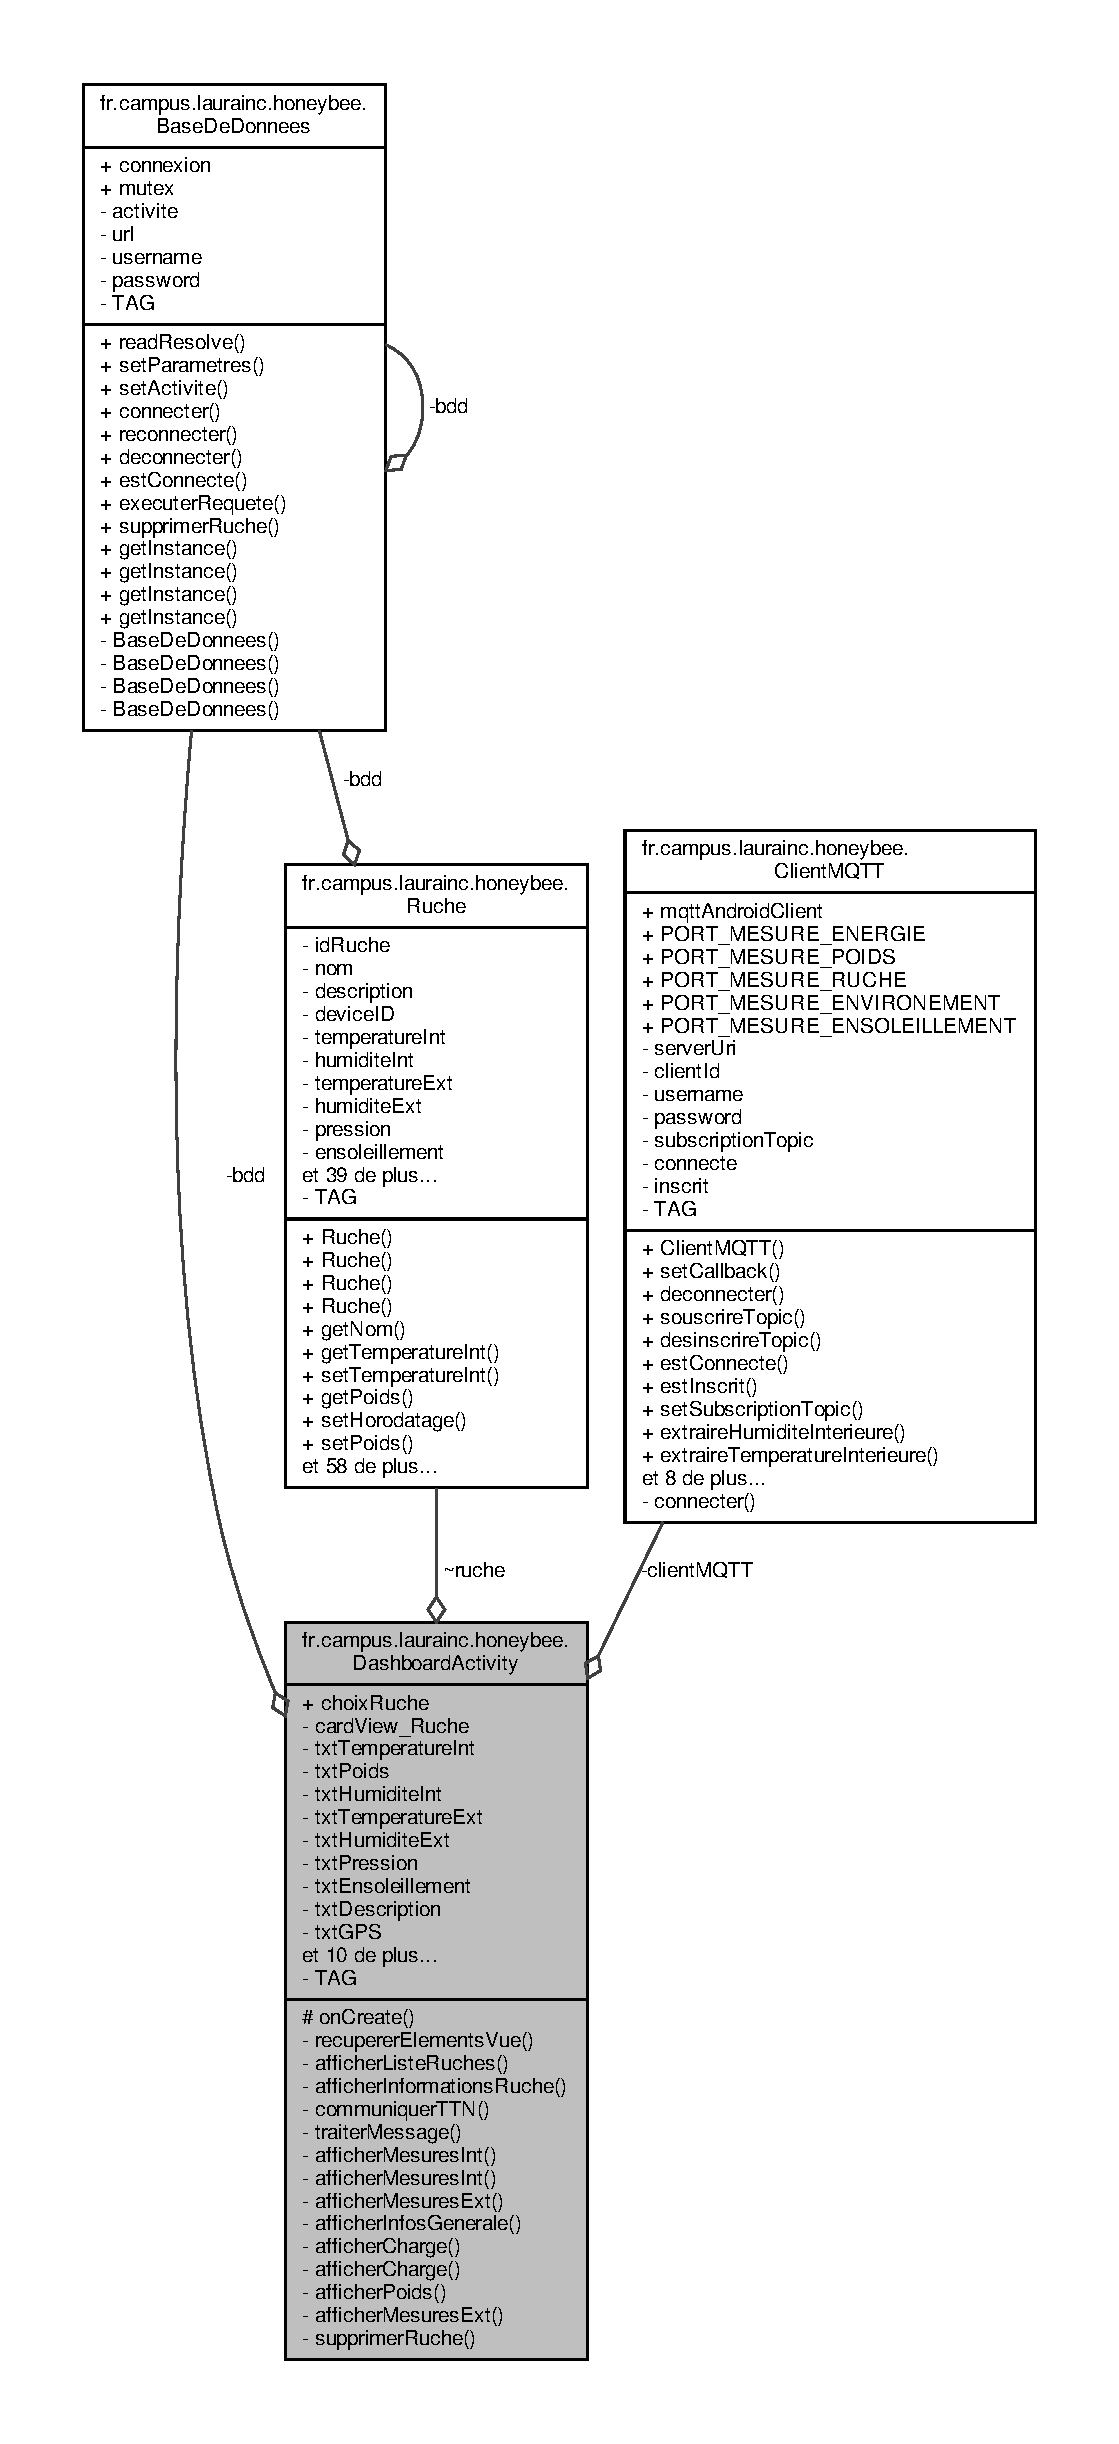
\includegraphics[height=550pt]{classfr_1_1campus_1_1laurainc_1_1honeybee_1_1_dashboard_activity__coll__graph}
\end{center}
\end{figure}
\subsubsection*{Attributs publics}
\begin{DoxyCompactItemize}
\item 
Spinner \hyperlink{classfr_1_1campus_1_1laurainc_1_1honeybee_1_1_dashboard_activity_ad3a78115526cf2cf371e6af8eb1b6b72}{choix\+Ruche}
\end{DoxyCompactItemize}
\subsubsection*{Fonctions membres protégées}
\begin{DoxyCompactItemize}
\item 
void \hyperlink{classfr_1_1campus_1_1laurainc_1_1honeybee_1_1_dashboard_activity_a8a6794a48e1b328dfc58d9d1c9237d79}{on\+Create} (Bundle saved\+Instance\+State)
\end{DoxyCompactItemize}
\subsubsection*{Fonctions membres privées}
\begin{DoxyCompactItemize}
\item 
void \hyperlink{classfr_1_1campus_1_1laurainc_1_1honeybee_1_1_dashboard_activity_a2ab46c5580913347e2dd18976be5900a}{recuperer\+Elements\+Vue} ()
\item 
void \hyperlink{classfr_1_1campus_1_1laurainc_1_1honeybee_1_1_dashboard_activity_aeb7cdaf69c379e2b070e290130199543}{afficher\+Liste\+Ruches} ()
\item 
void \hyperlink{classfr_1_1campus_1_1laurainc_1_1honeybee_1_1_dashboard_activity_a88f00531bee33bd6c47b33f5ac4df9ed}{afficher\+Informations\+Ruche} ()
\begin{DoxyCompactList}\small\item\em Affichage des informations d\textquotesingle{}une ruche dans la vue. \end{DoxyCompactList}\item 
void \hyperlink{classfr_1_1campus_1_1laurainc_1_1honeybee_1_1_dashboard_activity_abfefd572745e1034a025bc836812ae4f}{communiquer\+T\+TN} (String device\+ID)
\item 
void \hyperlink{classfr_1_1campus_1_1laurainc_1_1honeybee_1_1_dashboard_activity_a50d4c14e993ff1779ae5dce8cee11216}{traiter\+Message} (Mqtt\+Message mqtt\+Message)
\item 
void \hyperlink{classfr_1_1campus_1_1laurainc_1_1honeybee_1_1_dashboard_activity_aa177b8212619dec95e0a8eae4dbc867d}{afficher\+Mesures\+Int} (double temperature\+Interieure, double humidite\+Interieure, String Horodatage)
\item 
void \hyperlink{classfr_1_1campus_1_1laurainc_1_1honeybee_1_1_dashboard_activity_a4cc45d2f5c203313baaac3310d91e4be}{afficher\+Mesures\+Int} (double temperature\+Interieure, double humidite\+Interieure, double poids)
\item 
void \hyperlink{classfr_1_1campus_1_1laurainc_1_1honeybee_1_1_dashboard_activity_afffb9de4776b6c6cea676a08251a58ba}{afficher\+Mesures\+Ext} (double temperature\+Exterieure, double humidite\+Exterieure, double pression, double ensoleillement)
\item 
void \hyperlink{classfr_1_1campus_1_1laurainc_1_1honeybee_1_1_dashboard_activity_aaa61ed43c60c82f934647f15a38792cd}{afficher\+Infos\+Generale} (String description, String longitude, String latitude)
\item 
void \hyperlink{classfr_1_1campus_1_1laurainc_1_1honeybee_1_1_dashboard_activity_a13e1d8016723e33b6245e9e3063c8a4f}{afficher\+Charge} (int charge)
\item 
void \hyperlink{classfr_1_1campus_1_1laurainc_1_1honeybee_1_1_dashboard_activity_a8e57cfad2c497ab377ee6b7133ca6f18}{afficher\+Charge} (int charge, String horodatage)
\item 
void \hyperlink{classfr_1_1campus_1_1laurainc_1_1honeybee_1_1_dashboard_activity_a13786896440cb102e03bd5ac4f54c3d8}{afficher\+Poids} (int Poids, String Horodatage)
\item 
void \hyperlink{classfr_1_1campus_1_1laurainc_1_1honeybee_1_1_dashboard_activity_a0aef24c78a074282c20938eb2a665c8b}{afficher\+Mesures\+Ext} (double Humidite, double Temperature, double Pression, String Horodatage)
\item 
void \hyperlink{classfr_1_1campus_1_1laurainc_1_1honeybee_1_1_dashboard_activity_ae77451bd85101ed42644c2421cd2234f}{supprimer\+Ruche} ()
\end{DoxyCompactItemize}
\subsubsection*{Attributs privés}
\begin{DoxyCompactItemize}
\item 
\hyperlink{classfr_1_1campus_1_1laurainc_1_1honeybee_1_1_base_de_donnees}{Base\+De\+Donnees} \hyperlink{classfr_1_1campus_1_1laurainc_1_1honeybee_1_1_dashboard_activity_ac091db6a886cd65c54b8596c95b87d37}{bdd} = null
\begin{DoxyCompactList}\small\item\em l\textquotesingle{}objet permettant un accès à la base de données My\+S\+QL \end{DoxyCompactList}\item 
\hyperlink{classfr_1_1campus_1_1laurainc_1_1honeybee_1_1_client_m_q_t_t}{Client\+M\+Q\+TT} \hyperlink{classfr_1_1campus_1_1laurainc_1_1honeybee_1_1_dashboard_activity_ac72bac3feefe69341b1785a0133e1de8}{client\+M\+Q\+TT} = null
\item 
Card\+View \hyperlink{classfr_1_1campus_1_1laurainc_1_1honeybee_1_1_dashboard_activity_a2a213710fbe974be3a40fd6afecbd315}{card\+View\+\_\+\+Ruche}
\begin{DoxyCompactList}\small\item\em la vue contenant les informations générales de la ruche \end{DoxyCompactList}\item 
Text\+View \hyperlink{classfr_1_1campus_1_1laurainc_1_1honeybee_1_1_dashboard_activity_a336bd6552e6dc70bb2f9a92afd2fbdbe}{txt\+Temperature\+Int}
\item 
Text\+View \hyperlink{classfr_1_1campus_1_1laurainc_1_1honeybee_1_1_dashboard_activity_a1254223ab3507ce611d3244a43e8e14b}{txt\+Poids}
\item 
Text\+View \hyperlink{classfr_1_1campus_1_1laurainc_1_1honeybee_1_1_dashboard_activity_afb520230eefb68b38b2c12a2e57fb437}{txt\+Humidite\+Int}
\item 
Text\+View \hyperlink{classfr_1_1campus_1_1laurainc_1_1honeybee_1_1_dashboard_activity_a4a5b8ca6b359020d60e43c349c2538c3}{txt\+Temperature\+Ext}
\item 
Text\+View \hyperlink{classfr_1_1campus_1_1laurainc_1_1honeybee_1_1_dashboard_activity_a172fbb18fee80670357fe9ff8e2be62d}{txt\+Humidite\+Ext}
\item 
Text\+View \hyperlink{classfr_1_1campus_1_1laurainc_1_1honeybee_1_1_dashboard_activity_a0fc400e7bdb6580221af34a9d677e15b}{txt\+Pression}
\item 
Text\+View \hyperlink{classfr_1_1campus_1_1laurainc_1_1honeybee_1_1_dashboard_activity_aab4b50b607051748d695f8062e21e56e}{txt\+Ensoleillement}
\item 
Text\+View \hyperlink{classfr_1_1campus_1_1laurainc_1_1honeybee_1_1_dashboard_activity_a25b7b3ebb01b0a78ed4935f7881c89ab}{txt\+Description}
\item 
Text\+View \hyperlink{classfr_1_1campus_1_1laurainc_1_1honeybee_1_1_dashboard_activity_a0742bf6c7661b82f22ed90db43203029}{txt\+G\+PS}
\item 
Text\+View \hyperlink{classfr_1_1campus_1_1laurainc_1_1honeybee_1_1_dashboard_activity_a00185be7c66330a5a55881125fe5e400}{txt\+Charge}
\item 
Text\+View \hyperlink{classfr_1_1campus_1_1laurainc_1_1honeybee_1_1_dashboard_activity_abd1bc0732518150012172aaeee6e059b}{txt\+Alertes}
\item 
Image\+View \hyperlink{classfr_1_1campus_1_1laurainc_1_1honeybee_1_1_dashboard_activity_a2f9d67ea169a7cd9969d0fbe30e77fbc}{img\+Charge}
\item 
Image\+View \hyperlink{classfr_1_1campus_1_1laurainc_1_1honeybee_1_1_dashboard_activity_a99952672b3fddf694d15b817a1f933ab}{carte}
\item 
Button \hyperlink{classfr_1_1campus_1_1laurainc_1_1honeybee_1_1_dashboard_activity_a4170811fcbd865749a176f2c5c6ba617}{graphique}
\item 
Text\+View \hyperlink{classfr_1_1campus_1_1laurainc_1_1honeybee_1_1_dashboard_activity_a13c39ae74cce0c7f40b1d67e71d145cb}{donnees\+T\+TN}
\item 
Text\+View \hyperlink{classfr_1_1campus_1_1laurainc_1_1honeybee_1_1_dashboard_activity_a441403e9cd9a95a230d48b86090c4903}{txt\+Horodatage}
\item 
Floating\+Action\+Button \hyperlink{classfr_1_1campus_1_1laurainc_1_1honeybee_1_1_dashboard_activity_adeac9187a698545c246d039630bacd13}{bouton\+Supprimer\+Ruche}
\item 
Array\+List$<$ String $>$ \hyperlink{classfr_1_1campus_1_1laurainc_1_1honeybee_1_1_dashboard_activity_a85c92d113540b2ae3c20077050f1a90b}{mes\+Ruches}
\item 
final Handler \hyperlink{classfr_1_1campus_1_1laurainc_1_1honeybee_1_1_dashboard_activity_a7dd06030cd3afe35ace9a5e2f9e789dd}{handler}
\end{DoxyCompactItemize}
\subsubsection*{Attributs privés statiques}
\begin{DoxyCompactItemize}
\item 
static final String \hyperlink{classfr_1_1campus_1_1laurainc_1_1honeybee_1_1_dashboard_activity_a716b8b0ff7279634ec5d3079ddf5d840}{T\+AG} = \char`\"{}Dashboard\+Activity\char`\"{}
\begin{DoxyCompactList}\small\item\em le T\+AG de la classe pour les logs \end{DoxyCompactList}\end{DoxyCompactItemize}


\subsubsection{Documentation des fonctions membres}
\mbox{\Hypertarget{classfr_1_1campus_1_1laurainc_1_1honeybee_1_1_dashboard_activity_a13e1d8016723e33b6245e9e3063c8a4f}\label{classfr_1_1campus_1_1laurainc_1_1honeybee_1_1_dashboard_activity_a13e1d8016723e33b6245e9e3063c8a4f}} 
\index{fr\+::campus\+::laurainc\+::honeybee\+::\+Dashboard\+Activity@{fr\+::campus\+::laurainc\+::honeybee\+::\+Dashboard\+Activity}!afficher\+Charge@{afficher\+Charge}}
\index{afficher\+Charge@{afficher\+Charge}!fr\+::campus\+::laurainc\+::honeybee\+::\+Dashboard\+Activity@{fr\+::campus\+::laurainc\+::honeybee\+::\+Dashboard\+Activity}}
\paragraph{\texorpdfstring{afficher\+Charge()}{afficherCharge()}\hspace{0.1cm}{\footnotesize\ttfamily [1/2]}}
{\footnotesize\ttfamily void fr.\+campus.\+laurainc.\+honeybee.\+Dashboard\+Activity.\+afficher\+Charge (\begin{DoxyParamCaption}\item[{int}]{charge }\end{DoxyParamCaption})\hspace{0.3cm}{\ttfamily [private]}}



Référencé par \hyperlink{classfr_1_1campus_1_1laurainc_1_1honeybee_1_1_dashboard_activity_a88f00531bee33bd6c47b33f5ac4df9ed}{fr.\+campus.\+laurainc.\+honeybee.\+Dashboard\+Activity.\+afficher\+Informations\+Ruche()}, et \hyperlink{classfr_1_1campus_1_1laurainc_1_1honeybee_1_1_dashboard_activity_a50d4c14e993ff1779ae5dce8cee11216}{fr.\+campus.\+laurainc.\+honeybee.\+Dashboard\+Activity.\+traiter\+Message()}.


\begin{DoxyCode}
00296     \{
00297         \hyperlink{classfr_1_1campus_1_1laurainc_1_1honeybee_1_1_dashboard_activity_a00185be7c66330a5a55881125fe5e400}{txtCharge}.setText(valueOf(charge) + \textcolor{stringliteral}{" %"});
00298         \textcolor{keywordflow}{if} (charge > 85)
00299             \hyperlink{classfr_1_1campus_1_1laurainc_1_1honeybee_1_1_dashboard_activity_a2f9d67ea169a7cd9969d0fbe30e77fbc}{imgCharge}.setImageResource(R.drawable.battery1);
00300         \textcolor{keywordflow}{else} \textcolor{keywordflow}{if} (charge <= 85 && charge > 60)
00301             \hyperlink{classfr_1_1campus_1_1laurainc_1_1honeybee_1_1_dashboard_activity_a2f9d67ea169a7cd9969d0fbe30e77fbc}{imgCharge}.setImageResource(R.drawable.battery);
00302         \textcolor{keywordflow}{else} \textcolor{keywordflow}{if} (charge <= 60 && charge > 35)
00303             \hyperlink{classfr_1_1campus_1_1laurainc_1_1honeybee_1_1_dashboard_activity_a2f9d67ea169a7cd9969d0fbe30e77fbc}{imgCharge}.setImageResource(R.drawable.battery3);
00304         \textcolor{keywordflow}{else}
00305             \hyperlink{classfr_1_1campus_1_1laurainc_1_1honeybee_1_1_dashboard_activity_a2f9d67ea169a7cd9969d0fbe30e77fbc}{imgCharge}.setImageResource(R.drawable.battery2);
00306     \}
\end{DoxyCode}
\mbox{\Hypertarget{classfr_1_1campus_1_1laurainc_1_1honeybee_1_1_dashboard_activity_a8e57cfad2c497ab377ee6b7133ca6f18}\label{classfr_1_1campus_1_1laurainc_1_1honeybee_1_1_dashboard_activity_a8e57cfad2c497ab377ee6b7133ca6f18}} 
\index{fr\+::campus\+::laurainc\+::honeybee\+::\+Dashboard\+Activity@{fr\+::campus\+::laurainc\+::honeybee\+::\+Dashboard\+Activity}!afficher\+Charge@{afficher\+Charge}}
\index{afficher\+Charge@{afficher\+Charge}!fr\+::campus\+::laurainc\+::honeybee\+::\+Dashboard\+Activity@{fr\+::campus\+::laurainc\+::honeybee\+::\+Dashboard\+Activity}}
\paragraph{\texorpdfstring{afficher\+Charge()}{afficherCharge()}\hspace{0.1cm}{\footnotesize\ttfamily [2/2]}}
{\footnotesize\ttfamily void fr.\+campus.\+laurainc.\+honeybee.\+Dashboard\+Activity.\+afficher\+Charge (\begin{DoxyParamCaption}\item[{int}]{charge,  }\item[{String}]{horodatage }\end{DoxyParamCaption})\hspace{0.3cm}{\ttfamily [private]}}


\begin{DoxyCode}
00309     \{
00310         \hyperlink{classfr_1_1campus_1_1laurainc_1_1honeybee_1_1_dashboard_activity_a00185be7c66330a5a55881125fe5e400}{txtCharge}.setText(valueOf(charge) + \textcolor{stringliteral}{" %"});
00311         \hyperlink{classfr_1_1campus_1_1laurainc_1_1honeybee_1_1_dashboard_activity_a441403e9cd9a95a230d48b86090c4903}{txtHorodatage}.setText(valueOf(horodatage));
00312         \textcolor{keywordflow}{if} (charge > 85)
00313             \hyperlink{classfr_1_1campus_1_1laurainc_1_1honeybee_1_1_dashboard_activity_a2f9d67ea169a7cd9969d0fbe30e77fbc}{imgCharge}.setImageResource(R.drawable.battery1);
00314         \textcolor{keywordflow}{else} \textcolor{keywordflow}{if} (charge <= 85 && charge > 60)
00315             \hyperlink{classfr_1_1campus_1_1laurainc_1_1honeybee_1_1_dashboard_activity_a2f9d67ea169a7cd9969d0fbe30e77fbc}{imgCharge}.setImageResource(R.drawable.battery);
00316         \textcolor{keywordflow}{else} \textcolor{keywordflow}{if} (charge <= 60 && charge > 35)
00317             \hyperlink{classfr_1_1campus_1_1laurainc_1_1honeybee_1_1_dashboard_activity_a2f9d67ea169a7cd9969d0fbe30e77fbc}{imgCharge}.setImageResource(R.drawable.battery3);
00318         \textcolor{keywordflow}{else}
00319             \hyperlink{classfr_1_1campus_1_1laurainc_1_1honeybee_1_1_dashboard_activity_a2f9d67ea169a7cd9969d0fbe30e77fbc}{imgCharge}.setImageResource(R.drawable.battery2);
00320     \}
\end{DoxyCode}
\mbox{\Hypertarget{classfr_1_1campus_1_1laurainc_1_1honeybee_1_1_dashboard_activity_a88f00531bee33bd6c47b33f5ac4df9ed}\label{classfr_1_1campus_1_1laurainc_1_1honeybee_1_1_dashboard_activity_a88f00531bee33bd6c47b33f5ac4df9ed}} 
\index{fr\+::campus\+::laurainc\+::honeybee\+::\+Dashboard\+Activity@{fr\+::campus\+::laurainc\+::honeybee\+::\+Dashboard\+Activity}!afficher\+Informations\+Ruche@{afficher\+Informations\+Ruche}}
\index{afficher\+Informations\+Ruche@{afficher\+Informations\+Ruche}!fr\+::campus\+::laurainc\+::honeybee\+::\+Dashboard\+Activity@{fr\+::campus\+::laurainc\+::honeybee\+::\+Dashboard\+Activity}}
\paragraph{\texorpdfstring{afficher\+Informations\+Ruche()}{afficherInformationsRuche()}}
{\footnotesize\ttfamily fr.\+campus.\+laurainc.\+honeybee.\+Dashboard\+Activity.\+afficher\+Informations\+Ruche (\begin{DoxyParamCaption}{ }\end{DoxyParamCaption})\hspace{0.3cm}{\ttfamily [private]}}



Références \hyperlink{classfr_1_1campus_1_1laurainc_1_1honeybee_1_1_dashboard_activity_a13e1d8016723e33b6245e9e3063c8a4f}{fr.\+campus.\+laurainc.\+honeybee.\+Dashboard\+Activity.\+afficher\+Charge()}, \hyperlink{classfr_1_1campus_1_1laurainc_1_1honeybee_1_1_dashboard_activity_aaa61ed43c60c82f934647f15a38792cd}{fr.\+campus.\+laurainc.\+honeybee.\+Dashboard\+Activity.\+afficher\+Infos\+Generale()}, \hyperlink{classfr_1_1campus_1_1laurainc_1_1honeybee_1_1_dashboard_activity_afffb9de4776b6c6cea676a08251a58ba}{fr.\+campus.\+laurainc.\+honeybee.\+Dashboard\+Activity.\+afficher\+Mesures\+Ext()}, \hyperlink{classfr_1_1campus_1_1laurainc_1_1honeybee_1_1_dashboard_activity_aa177b8212619dec95e0a8eae4dbc867d}{fr.\+campus.\+laurainc.\+honeybee.\+Dashboard\+Activity.\+afficher\+Mesures\+Int()}, \hyperlink{classfr_1_1campus_1_1laurainc_1_1honeybee_1_1_dashboard_activity_abfefd572745e1034a025bc836812ae4f}{fr.\+campus.\+laurainc.\+honeybee.\+Dashboard\+Activity.\+communiquer\+T\+T\+N()}, \hyperlink{classfr_1_1campus_1_1laurainc_1_1honeybee_1_1_ruche_a28fe3a64c8aaf28cf15a96a8aa37e23b}{fr.\+campus.\+laurainc.\+honeybee.\+Ruche.\+get\+Charge()}, \hyperlink{classfr_1_1campus_1_1laurainc_1_1honeybee_1_1_ruche_ade21eb84d2a34d71cc2e89134b79cfd2}{fr.\+campus.\+laurainc.\+honeybee.\+Ruche.\+get\+Description()}, \hyperlink{classfr_1_1campus_1_1laurainc_1_1honeybee_1_1_ruche_a0cbf5aacc51f6a0fc5bd9def0f1a32c7}{fr.\+campus.\+laurainc.\+honeybee.\+Ruche.\+get\+Device\+I\+D()}, \hyperlink{classfr_1_1campus_1_1laurainc_1_1honeybee_1_1_ruche_a18a40461d368f06fd0532bfa1b63b868}{fr.\+campus.\+laurainc.\+honeybee.\+Ruche.\+get\+Ensoleillement()}, \hyperlink{classfr_1_1campus_1_1laurainc_1_1honeybee_1_1_ruche_a8e3b05a40fa1a699b7ffc1d15a7f6e31}{fr.\+campus.\+laurainc.\+honeybee.\+Ruche.\+get\+Humidite\+Ext()}, \hyperlink{classfr_1_1campus_1_1laurainc_1_1honeybee_1_1_ruche_ab4f2b99dbdcb4cfcb81827f294ffeb4a}{fr.\+campus.\+laurainc.\+honeybee.\+Ruche.\+get\+Humidite\+Int()}, \hyperlink{classfr_1_1campus_1_1laurainc_1_1honeybee_1_1_ruche_a3f03f6958a9251f72e60e45a6b8eb65c}{fr.\+campus.\+laurainc.\+honeybee.\+Ruche.\+get\+Latitude()}, \hyperlink{classfr_1_1campus_1_1laurainc_1_1honeybee_1_1_ruche_a45b3656e287e168f17fdd1b9ec5fbca1}{fr.\+campus.\+laurainc.\+honeybee.\+Ruche.\+get\+Longitude()}, \hyperlink{classfr_1_1campus_1_1laurainc_1_1honeybee_1_1_ruche_a0db4200faed3952a50f63fa7634be39b}{fr.\+campus.\+laurainc.\+honeybee.\+Ruche.\+get\+Nom()}, \hyperlink{classfr_1_1campus_1_1laurainc_1_1honeybee_1_1_ruche_a1dce2bd8e8de34d082abd36eab6693d3}{fr.\+campus.\+laurainc.\+honeybee.\+Ruche.\+get\+Poids()}, \hyperlink{classfr_1_1campus_1_1laurainc_1_1honeybee_1_1_ruche_a9d94748ece29463c420e93e0e7aa7acd}{fr.\+campus.\+laurainc.\+honeybee.\+Ruche.\+get\+Pression()}, \hyperlink{classfr_1_1campus_1_1laurainc_1_1honeybee_1_1_ruche_ac42e5846fb470d9ac9112c20c8679980}{fr.\+campus.\+laurainc.\+honeybee.\+Ruche.\+get\+Temperature\+Ext()}, et \hyperlink{classfr_1_1campus_1_1laurainc_1_1honeybee_1_1_ruche_aca5e489525d7f0cba7741a0d1803c5e5}{fr.\+campus.\+laurainc.\+honeybee.\+Ruche.\+get\+Temperature\+Int()}.


\begin{DoxyCode}
00159     \{
00160         \textcolor{keywordflow}{if}(ruche != null)
00161         \{
00162             Log.d(\hyperlink{classfr_1_1campus_1_1laurainc_1_1honeybee_1_1_dashboard_activity_a716b8b0ff7279634ec5d3079ddf5d840}{TAG}, \textcolor{stringliteral}{"Ruche : "} + ruche.\hyperlink{classfr_1_1campus_1_1laurainc_1_1honeybee_1_1_ruche_a0db4200faed3952a50f63fa7634be39b}{getNom}());
00163             \hyperlink{classfr_1_1campus_1_1laurainc_1_1honeybee_1_1_dashboard_activity_a13e1d8016723e33b6245e9e3063c8a4f}{afficherCharge}(ruche.\hyperlink{classfr_1_1campus_1_1laurainc_1_1honeybee_1_1_ruche_a28fe3a64c8aaf28cf15a96a8aa37e23b}{getCharge}());
00164             \hyperlink{classfr_1_1campus_1_1laurainc_1_1honeybee_1_1_dashboard_activity_aaa61ed43c60c82f934647f15a38792cd}{afficherInfosGenerale}(ruche.\hyperlink{classfr_1_1campus_1_1laurainc_1_1honeybee_1_1_ruche_ade21eb84d2a34d71cc2e89134b79cfd2}{getDescription}(), ruche.
      \hyperlink{classfr_1_1campus_1_1laurainc_1_1honeybee_1_1_ruche_a45b3656e287e168f17fdd1b9ec5fbca1}{getLongitude}(), ruche.\hyperlink{classfr_1_1campus_1_1laurainc_1_1honeybee_1_1_ruche_a3f03f6958a9251f72e60e45a6b8eb65c}{getLatitude}());
00165             \hyperlink{classfr_1_1campus_1_1laurainc_1_1honeybee_1_1_dashboard_activity_aa177b8212619dec95e0a8eae4dbc867d}{afficherMesuresInt}(ruche.\hyperlink{classfr_1_1campus_1_1laurainc_1_1honeybee_1_1_ruche_aca5e489525d7f0cba7741a0d1803c5e5}{getTemperatureInt}(), ruche.
      \hyperlink{classfr_1_1campus_1_1laurainc_1_1honeybee_1_1_ruche_ab4f2b99dbdcb4cfcb81827f294ffeb4a}{getHumiditeInt}(), ruche.\hyperlink{classfr_1_1campus_1_1laurainc_1_1honeybee_1_1_ruche_a1dce2bd8e8de34d082abd36eab6693d3}{getPoids}());
00166             Log.d(\hyperlink{classfr_1_1campus_1_1laurainc_1_1honeybee_1_1_dashboard_activity_a716b8b0ff7279634ec5d3079ddf5d840}{TAG}, \textcolor{stringliteral}{"Affichage des données intérieures"});
00167             \hyperlink{classfr_1_1campus_1_1laurainc_1_1honeybee_1_1_dashboard_activity_afffb9de4776b6c6cea676a08251a58ba}{afficherMesuresExt}(ruche.\hyperlink{classfr_1_1campus_1_1laurainc_1_1honeybee_1_1_ruche_ac42e5846fb470d9ac9112c20c8679980}{getTemperatureExt}(), ruche.
      \hyperlink{classfr_1_1campus_1_1laurainc_1_1honeybee_1_1_ruche_a8e3b05a40fa1a699b7ffc1d15a7f6e31}{getHumiditeExt}(), ruche.\hyperlink{classfr_1_1campus_1_1laurainc_1_1honeybee_1_1_ruche_a9d94748ece29463c420e93e0e7aa7acd}{getPression}(), ruche.
      \hyperlink{classfr_1_1campus_1_1laurainc_1_1honeybee_1_1_ruche_a18a40461d368f06fd0532bfa1b63b868}{getEnsoleillement}());
00168             Log.d(\hyperlink{classfr_1_1campus_1_1laurainc_1_1honeybee_1_1_dashboard_activity_a716b8b0ff7279634ec5d3079ddf5d840}{TAG}, \textcolor{stringliteral}{"Affichage des données extérieures"});
00169             \hyperlink{classfr_1_1campus_1_1laurainc_1_1honeybee_1_1_dashboard_activity_a13c39ae74cce0c7f40b1d67e71d145cb}{donneesTTN}.setText(\textcolor{stringliteral}{"En attente des données du serveur TTN ..."});
00170             String topic = \textcolor{stringliteral}{"mes\_ruches/devices/"} + ruche.\hyperlink{classfr_1_1campus_1_1laurainc_1_1honeybee_1_1_ruche_a0cbf5aacc51f6a0fc5bd9def0f1a32c7}{getDeviceID}() + \textcolor{stringliteral}{"/up"};
00171             \hyperlink{classfr_1_1campus_1_1laurainc_1_1honeybee_1_1_dashboard_activity_ac72bac3feefe69341b1785a0133e1de8}{clientMQTT} = \textcolor{keyword}{new} ClientMQTT(ruche.\hyperlink{classfr_1_1campus_1_1laurainc_1_1honeybee_1_1_ruche_a0cbf5aacc51f6a0fc5bd9def0f1a32c7}{getDeviceID}(), topic, 
      getApplicationContext());
00172             \hyperlink{classfr_1_1campus_1_1laurainc_1_1honeybee_1_1_dashboard_activity_abfefd572745e1034a025bc836812ae4f}{communiquerTTN}(ruche.\hyperlink{classfr_1_1campus_1_1laurainc_1_1honeybee_1_1_ruche_a0cbf5aacc51f6a0fc5bd9def0f1a32c7}{getDeviceID}());
00173         \}
00174     \}
\end{DoxyCode}
\mbox{\Hypertarget{classfr_1_1campus_1_1laurainc_1_1honeybee_1_1_dashboard_activity_aaa61ed43c60c82f934647f15a38792cd}\label{classfr_1_1campus_1_1laurainc_1_1honeybee_1_1_dashboard_activity_aaa61ed43c60c82f934647f15a38792cd}} 
\index{fr\+::campus\+::laurainc\+::honeybee\+::\+Dashboard\+Activity@{fr\+::campus\+::laurainc\+::honeybee\+::\+Dashboard\+Activity}!afficher\+Infos\+Generale@{afficher\+Infos\+Generale}}
\index{afficher\+Infos\+Generale@{afficher\+Infos\+Generale}!fr\+::campus\+::laurainc\+::honeybee\+::\+Dashboard\+Activity@{fr\+::campus\+::laurainc\+::honeybee\+::\+Dashboard\+Activity}}
\paragraph{\texorpdfstring{afficher\+Infos\+Generale()}{afficherInfosGenerale()}}
{\footnotesize\ttfamily void fr.\+campus.\+laurainc.\+honeybee.\+Dashboard\+Activity.\+afficher\+Infos\+Generale (\begin{DoxyParamCaption}\item[{String}]{description,  }\item[{String}]{longitude,  }\item[{String}]{latitude }\end{DoxyParamCaption})\hspace{0.3cm}{\ttfamily [private]}}



Référencé par \hyperlink{classfr_1_1campus_1_1laurainc_1_1honeybee_1_1_dashboard_activity_a88f00531bee33bd6c47b33f5ac4df9ed}{fr.\+campus.\+laurainc.\+honeybee.\+Dashboard\+Activity.\+afficher\+Informations\+Ruche()}.


\begin{DoxyCode}
00290     \{
00291         \hyperlink{classfr_1_1campus_1_1laurainc_1_1honeybee_1_1_dashboard_activity_a25b7b3ebb01b0a78ed4935f7881c89ab}{txtDescription}.setText(description);
00292         \hyperlink{classfr_1_1campus_1_1laurainc_1_1honeybee_1_1_dashboard_activity_a0742bf6c7661b82f22ed90db43203029}{txtGPS}.setText(longitude + \textcolor{stringliteral}{", "} + latitude);
00293     \}
\end{DoxyCode}
\mbox{\Hypertarget{classfr_1_1campus_1_1laurainc_1_1honeybee_1_1_dashboard_activity_aeb7cdaf69c379e2b070e290130199543}\label{classfr_1_1campus_1_1laurainc_1_1honeybee_1_1_dashboard_activity_aeb7cdaf69c379e2b070e290130199543}} 
\index{fr\+::campus\+::laurainc\+::honeybee\+::\+Dashboard\+Activity@{fr\+::campus\+::laurainc\+::honeybee\+::\+Dashboard\+Activity}!afficher\+Liste\+Ruches@{afficher\+Liste\+Ruches}}
\index{afficher\+Liste\+Ruches@{afficher\+Liste\+Ruches}!fr\+::campus\+::laurainc\+::honeybee\+::\+Dashboard\+Activity@{fr\+::campus\+::laurainc\+::honeybee\+::\+Dashboard\+Activity}}
\paragraph{\texorpdfstring{afficher\+Liste\+Ruches()}{afficherListeRuches()}}
{\footnotesize\ttfamily void fr.\+campus.\+laurainc.\+honeybee.\+Dashboard\+Activity.\+afficher\+Liste\+Ruches (\begin{DoxyParamCaption}{ }\end{DoxyParamCaption})\hspace{0.3cm}{\ttfamily [private]}}



Références \hyperlink{classfr_1_1campus_1_1laurainc_1_1honeybee_1_1_client_m_q_t_t_af067ec55e00ec18a14e248279872242f}{fr.\+campus.\+laurainc.\+honeybee.\+Client\+M\+Q\+T\+T.\+deconnecter()}, \hyperlink{classfr_1_1campus_1_1laurainc_1_1honeybee_1_1_client_m_q_t_t_a06c30a7291f526d0bd9a47fccb3ac1ad}{fr.\+campus.\+laurainc.\+honeybee.\+Client\+M\+Q\+T\+T.\+est\+Connecte()}, \hyperlink{classfr_1_1campus_1_1laurainc_1_1honeybee_1_1_ruche_a7108fb412c0628d3966aa8c76fd9e2b7}{fr.\+campus.\+laurainc.\+honeybee.\+Ruche.\+get\+Liste\+Ruches()}, \hyperlink{classfr_1_1campus_1_1laurainc_1_1honeybee_1_1_dashboard_activity_a7dd06030cd3afe35ace9a5e2f9e789dd}{fr.\+campus.\+laurainc.\+honeybee.\+Dashboard\+Activity.\+handler}, et \hyperlink{classfr_1_1campus_1_1laurainc_1_1honeybee_1_1_dashboard_activity_a85c92d113540b2ae3c20077050f1a90b}{fr.\+campus.\+laurainc.\+honeybee.\+Dashboard\+Activity.\+mes\+Ruches}.


\begin{DoxyCode}
00120                                        \{
00121         \hyperlink{classfr_1_1campus_1_1laurainc_1_1honeybee_1_1_dashboard_activity_a85c92d113540b2ae3c20077050f1a90b}{mesRuches} = ruche.\hyperlink{classfr_1_1campus_1_1laurainc_1_1honeybee_1_1_ruche_a7108fb412c0628d3966aa8c76fd9e2b7}{getListeRuches}();
00122         ArrayAdapter<String> adapter = \textcolor{keyword}{new} ArrayAdapter<String>(\textcolor{keyword}{this}, R.layout.item\_spinner ,
      \hyperlink{classfr_1_1campus_1_1laurainc_1_1honeybee_1_1_dashboard_activity_a85c92d113540b2ae3c20077050f1a90b}{mesRuches});
00123         adapter.setDropDownViewResource(android.R.layout.simple\_spinner\_dropdown\_item);
00124         \hyperlink{classfr_1_1campus_1_1laurainc_1_1honeybee_1_1_dashboard_activity_ad3a78115526cf2cf371e6af8eb1b6b72}{choixRuche}.setAdapter(adapter);
00125         \hyperlink{classfr_1_1campus_1_1laurainc_1_1honeybee_1_1_dashboard_activity_ad3a78115526cf2cf371e6af8eb1b6b72}{choixRuche}.setSelection(0);
00126         \textcolor{comment}{//adapter.setNotifyOnChange(true);}
00127 
00128         \hyperlink{classfr_1_1campus_1_1laurainc_1_1honeybee_1_1_dashboard_activity_ad3a78115526cf2cf371e6af8eb1b6b72}{choixRuche}.setOnItemSelectedListener(\textcolor{keyword}{new} AdapterView.OnItemSelectedListener()
00129         \{
00130             @Override
00131             \textcolor{keyword}{public} \textcolor{keywordtype}{void} onItemSelected(AdapterView<?> arg0, View arg1, \textcolor{keywordtype}{int} position, \textcolor{keywordtype}{long} \textcolor{keywordtype}{id})
00132             \{
00133                 Toast.makeText(getBaseContext(), \hyperlink{classfr_1_1campus_1_1laurainc_1_1honeybee_1_1_dashboard_activity_a85c92d113540b2ae3c20077050f1a90b}{mesRuches}.get(position), Toast.LENGTH\_SHORT).show
      ();
00134                 Log.d(\hyperlink{classfr_1_1campus_1_1laurainc_1_1honeybee_1_1_dashboard_activity_a716b8b0ff7279634ec5d3079ddf5d840}{TAG}, \textcolor{stringliteral}{"position : "} + position);
00135                 \textcolor{keywordflow}{if}(\hyperlink{classfr_1_1campus_1_1laurainc_1_1honeybee_1_1_dashboard_activity_ac72bac3feefe69341b1785a0133e1de8}{clientMQTT} != null)
00136                 \{
00137                     \textcolor{keywordflow}{if}(\hyperlink{classfr_1_1campus_1_1laurainc_1_1honeybee_1_1_dashboard_activity_ac72bac3feefe69341b1785a0133e1de8}{clientMQTT}.\hyperlink{classfr_1_1campus_1_1laurainc_1_1honeybee_1_1_client_m_q_t_t_a06c30a7291f526d0bd9a47fccb3ac1ad}{estConnecte}())
00138                         \hyperlink{classfr_1_1campus_1_1laurainc_1_1honeybee_1_1_dashboard_activity_ac72bac3feefe69341b1785a0133e1de8}{clientMQTT}.\hyperlink{classfr_1_1campus_1_1laurainc_1_1honeybee_1_1_client_m_q_t_t_af067ec55e00ec18a14e248279872242f}{deconnecter}();
00139 
00140                 \}
00141                 \textcolor{comment}{// Instancie une ruche}
00142                 ruche = \textcolor{keyword}{new} \hyperlink{class_ruche}{Ruche}(\hyperlink{classfr_1_1campus_1_1laurainc_1_1honeybee_1_1_dashboard_activity_a85c92d113540b2ae3c20077050f1a90b}{mesRuches}.get(position), \hyperlink{classfr_1_1campus_1_1laurainc_1_1honeybee_1_1_dashboard_activity_a7dd06030cd3afe35ace9a5e2f9e789dd}{handler});
00143             \}
00144 
00145             @Override
00146             \textcolor{keyword}{public} \textcolor{keywordtype}{void} onNothingSelected(AdapterView<?> arg0)
00147             \{
00148                 \textcolor{comment}{// TODO Auto-generated method stub}
00149             \}
00150         \});
00151     \}
\end{DoxyCode}
\mbox{\Hypertarget{classfr_1_1campus_1_1laurainc_1_1honeybee_1_1_dashboard_activity_afffb9de4776b6c6cea676a08251a58ba}\label{classfr_1_1campus_1_1laurainc_1_1honeybee_1_1_dashboard_activity_afffb9de4776b6c6cea676a08251a58ba}} 
\index{fr\+::campus\+::laurainc\+::honeybee\+::\+Dashboard\+Activity@{fr\+::campus\+::laurainc\+::honeybee\+::\+Dashboard\+Activity}!afficher\+Mesures\+Ext@{afficher\+Mesures\+Ext}}
\index{afficher\+Mesures\+Ext@{afficher\+Mesures\+Ext}!fr\+::campus\+::laurainc\+::honeybee\+::\+Dashboard\+Activity@{fr\+::campus\+::laurainc\+::honeybee\+::\+Dashboard\+Activity}}
\paragraph{\texorpdfstring{afficher\+Mesures\+Ext()}{afficherMesuresExt()}\hspace{0.1cm}{\footnotesize\ttfamily [1/2]}}
{\footnotesize\ttfamily void fr.\+campus.\+laurainc.\+honeybee.\+Dashboard\+Activity.\+afficher\+Mesures\+Ext (\begin{DoxyParamCaption}\item[{double}]{temperature\+Exterieure,  }\item[{double}]{humidite\+Exterieure,  }\item[{double}]{pression,  }\item[{double}]{ensoleillement }\end{DoxyParamCaption})\hspace{0.3cm}{\ttfamily [private]}}



Référencé par \hyperlink{classfr_1_1campus_1_1laurainc_1_1honeybee_1_1_dashboard_activity_a88f00531bee33bd6c47b33f5ac4df9ed}{fr.\+campus.\+laurainc.\+honeybee.\+Dashboard\+Activity.\+afficher\+Informations\+Ruche()}, et \hyperlink{classfr_1_1campus_1_1laurainc_1_1honeybee_1_1_dashboard_activity_a50d4c14e993ff1779ae5dce8cee11216}{fr.\+campus.\+laurainc.\+honeybee.\+Dashboard\+Activity.\+traiter\+Message()}.


\begin{DoxyCode}
00282     \{
00283         \hyperlink{classfr_1_1campus_1_1laurainc_1_1honeybee_1_1_dashboard_activity_a4a5b8ca6b359020d60e43c349c2538c3}{txtTemperatureExt}.setText(valueOf(temperatureExterieure) + \textcolor{stringliteral}{" °C"});
00284         \hyperlink{classfr_1_1campus_1_1laurainc_1_1honeybee_1_1_dashboard_activity_a172fbb18fee80670357fe9ff8e2be62d}{txtHumiditeExt}.setText(valueOf(humiditeExterieure) + \textcolor{stringliteral}{" %"});
00285         \hyperlink{classfr_1_1campus_1_1laurainc_1_1honeybee_1_1_dashboard_activity_a0fc400e7bdb6580221af34a9d677e15b}{txtPression}.setText(valueOf(pression) + \textcolor{stringliteral}{" hPa"});
00286         \hyperlink{classfr_1_1campus_1_1laurainc_1_1honeybee_1_1_dashboard_activity_aab4b50b607051748d695f8062e21e56e}{txtEnsoleillement}.setText(valueOf(ensoleillement) + \textcolor{stringliteral}{" Watt/m²"});
00287     \}
\end{DoxyCode}
\mbox{\Hypertarget{classfr_1_1campus_1_1laurainc_1_1honeybee_1_1_dashboard_activity_a0aef24c78a074282c20938eb2a665c8b}\label{classfr_1_1campus_1_1laurainc_1_1honeybee_1_1_dashboard_activity_a0aef24c78a074282c20938eb2a665c8b}} 
\index{fr\+::campus\+::laurainc\+::honeybee\+::\+Dashboard\+Activity@{fr\+::campus\+::laurainc\+::honeybee\+::\+Dashboard\+Activity}!afficher\+Mesures\+Ext@{afficher\+Mesures\+Ext}}
\index{afficher\+Mesures\+Ext@{afficher\+Mesures\+Ext}!fr\+::campus\+::laurainc\+::honeybee\+::\+Dashboard\+Activity@{fr\+::campus\+::laurainc\+::honeybee\+::\+Dashboard\+Activity}}
\paragraph{\texorpdfstring{afficher\+Mesures\+Ext()}{afficherMesuresExt()}\hspace{0.1cm}{\footnotesize\ttfamily [2/2]}}
{\footnotesize\ttfamily void fr.\+campus.\+laurainc.\+honeybee.\+Dashboard\+Activity.\+afficher\+Mesures\+Ext (\begin{DoxyParamCaption}\item[{double}]{Humidite,  }\item[{double}]{Temperature,  }\item[{double}]{Pression,  }\item[{String}]{Horodatage }\end{DoxyParamCaption})\hspace{0.3cm}{\ttfamily [private]}}


\begin{DoxyCode}
00330     \{
00331         \hyperlink{classfr_1_1campus_1_1laurainc_1_1honeybee_1_1_dashboard_activity_a172fbb18fee80670357fe9ff8e2be62d}{txtHumiditeExt}.setText(valueOf(Humidite) + \textcolor{stringliteral}{" %"});
00332         \hyperlink{classfr_1_1campus_1_1laurainc_1_1honeybee_1_1_dashboard_activity_a4a5b8ca6b359020d60e43c349c2538c3}{txtTemperatureExt}.setText(valueOf(Temperature) + \textcolor{stringliteral}{" °C"});
00333         \hyperlink{classfr_1_1campus_1_1laurainc_1_1honeybee_1_1_dashboard_activity_a0fc400e7bdb6580221af34a9d677e15b}{txtPression}.setText(valueOf(Pression) + \textcolor{stringliteral}{" hPa"});
00334         \hyperlink{classfr_1_1campus_1_1laurainc_1_1honeybee_1_1_dashboard_activity_a441403e9cd9a95a230d48b86090c4903}{txtHorodatage}.setText(Horodatage);
00335     \}
\end{DoxyCode}
\mbox{\Hypertarget{classfr_1_1campus_1_1laurainc_1_1honeybee_1_1_dashboard_activity_aa177b8212619dec95e0a8eae4dbc867d}\label{classfr_1_1campus_1_1laurainc_1_1honeybee_1_1_dashboard_activity_aa177b8212619dec95e0a8eae4dbc867d}} 
\index{fr\+::campus\+::laurainc\+::honeybee\+::\+Dashboard\+Activity@{fr\+::campus\+::laurainc\+::honeybee\+::\+Dashboard\+Activity}!afficher\+Mesures\+Int@{afficher\+Mesures\+Int}}
\index{afficher\+Mesures\+Int@{afficher\+Mesures\+Int}!fr\+::campus\+::laurainc\+::honeybee\+::\+Dashboard\+Activity@{fr\+::campus\+::laurainc\+::honeybee\+::\+Dashboard\+Activity}}
\paragraph{\texorpdfstring{afficher\+Mesures\+Int()}{afficherMesuresInt()}\hspace{0.1cm}{\footnotesize\ttfamily [1/2]}}
{\footnotesize\ttfamily void fr.\+campus.\+laurainc.\+honeybee.\+Dashboard\+Activity.\+afficher\+Mesures\+Int (\begin{DoxyParamCaption}\item[{double}]{temperature\+Interieure,  }\item[{double}]{humidite\+Interieure,  }\item[{String}]{Horodatage }\end{DoxyParamCaption})\hspace{0.3cm}{\ttfamily [private]}}



Référencé par \hyperlink{classfr_1_1campus_1_1laurainc_1_1honeybee_1_1_dashboard_activity_a88f00531bee33bd6c47b33f5ac4df9ed}{fr.\+campus.\+laurainc.\+honeybee.\+Dashboard\+Activity.\+afficher\+Informations\+Ruche()}, et \hyperlink{classfr_1_1campus_1_1laurainc_1_1honeybee_1_1_dashboard_activity_a50d4c14e993ff1779ae5dce8cee11216}{fr.\+campus.\+laurainc.\+honeybee.\+Dashboard\+Activity.\+traiter\+Message()}.


\begin{DoxyCode}
00268     \{
00269         \hyperlink{classfr_1_1campus_1_1laurainc_1_1honeybee_1_1_dashboard_activity_a336bd6552e6dc70bb2f9a92afd2fbdbe}{txtTemperatureInt}.setText(valueOf(temperatureInterieure) + \textcolor{stringliteral}{" °C"});
00270         \hyperlink{classfr_1_1campus_1_1laurainc_1_1honeybee_1_1_dashboard_activity_afb520230eefb68b38b2c12a2e57fb437}{txtHumiditeInt}.setText(valueOf(humiditeInterieure) + \textcolor{stringliteral}{" %"});
00271         \hyperlink{classfr_1_1campus_1_1laurainc_1_1honeybee_1_1_dashboard_activity_a441403e9cd9a95a230d48b86090c4903}{txtHorodatage}.setText(Horodatage);
00272     \}
\end{DoxyCode}
\mbox{\Hypertarget{classfr_1_1campus_1_1laurainc_1_1honeybee_1_1_dashboard_activity_a4cc45d2f5c203313baaac3310d91e4be}\label{classfr_1_1campus_1_1laurainc_1_1honeybee_1_1_dashboard_activity_a4cc45d2f5c203313baaac3310d91e4be}} 
\index{fr\+::campus\+::laurainc\+::honeybee\+::\+Dashboard\+Activity@{fr\+::campus\+::laurainc\+::honeybee\+::\+Dashboard\+Activity}!afficher\+Mesures\+Int@{afficher\+Mesures\+Int}}
\index{afficher\+Mesures\+Int@{afficher\+Mesures\+Int}!fr\+::campus\+::laurainc\+::honeybee\+::\+Dashboard\+Activity@{fr\+::campus\+::laurainc\+::honeybee\+::\+Dashboard\+Activity}}
\paragraph{\texorpdfstring{afficher\+Mesures\+Int()}{afficherMesuresInt()}\hspace{0.1cm}{\footnotesize\ttfamily [2/2]}}
{\footnotesize\ttfamily void fr.\+campus.\+laurainc.\+honeybee.\+Dashboard\+Activity.\+afficher\+Mesures\+Int (\begin{DoxyParamCaption}\item[{double}]{temperature\+Interieure,  }\item[{double}]{humidite\+Interieure,  }\item[{double}]{poids }\end{DoxyParamCaption})\hspace{0.3cm}{\ttfamily [private]}}


\begin{DoxyCode}
00275     \{
00276         \hyperlink{classfr_1_1campus_1_1laurainc_1_1honeybee_1_1_dashboard_activity_a336bd6552e6dc70bb2f9a92afd2fbdbe}{txtTemperatureInt}.setText(valueOf(temperatureInterieure) + \textcolor{stringliteral}{" °C"});
00277         \hyperlink{classfr_1_1campus_1_1laurainc_1_1honeybee_1_1_dashboard_activity_afb520230eefb68b38b2c12a2e57fb437}{txtHumiditeInt}.setText(valueOf(humiditeInterieure) + \textcolor{stringliteral}{" %"});
00278         \hyperlink{classfr_1_1campus_1_1laurainc_1_1honeybee_1_1_dashboard_activity_a1254223ab3507ce611d3244a43e8e14b}{txtPoids}.setText(valueOf(poids) + \textcolor{stringliteral}{" Kg"});
00279     \}
\end{DoxyCode}
\mbox{\Hypertarget{classfr_1_1campus_1_1laurainc_1_1honeybee_1_1_dashboard_activity_a13786896440cb102e03bd5ac4f54c3d8}\label{classfr_1_1campus_1_1laurainc_1_1honeybee_1_1_dashboard_activity_a13786896440cb102e03bd5ac4f54c3d8}} 
\index{fr\+::campus\+::laurainc\+::honeybee\+::\+Dashboard\+Activity@{fr\+::campus\+::laurainc\+::honeybee\+::\+Dashboard\+Activity}!afficher\+Poids@{afficher\+Poids}}
\index{afficher\+Poids@{afficher\+Poids}!fr\+::campus\+::laurainc\+::honeybee\+::\+Dashboard\+Activity@{fr\+::campus\+::laurainc\+::honeybee\+::\+Dashboard\+Activity}}
\paragraph{\texorpdfstring{afficher\+Poids()}{afficherPoids()}}
{\footnotesize\ttfamily void fr.\+campus.\+laurainc.\+honeybee.\+Dashboard\+Activity.\+afficher\+Poids (\begin{DoxyParamCaption}\item[{int}]{Poids,  }\item[{String}]{Horodatage }\end{DoxyParamCaption})\hspace{0.3cm}{\ttfamily [private]}}



Références \hyperlink{classfr_1_1campus_1_1laurainc_1_1honeybee_1_1_client_m_q_t_t_a00ce9a2b07615c9337e452b5a51fedbe}{fr.\+campus.\+laurainc.\+honeybee.\+Client\+M\+Q\+T\+T.\+arrondir()}.



Référencé par \hyperlink{classfr_1_1campus_1_1laurainc_1_1honeybee_1_1_dashboard_activity_a50d4c14e993ff1779ae5dce8cee11216}{fr.\+campus.\+laurainc.\+honeybee.\+Dashboard\+Activity.\+traiter\+Message()}.


\begin{DoxyCode}
00323     \{
00324         \textcolor{keywordtype}{double} poidsKg = \hyperlink{classfr_1_1campus_1_1laurainc_1_1honeybee_1_1_dashboard_activity_ac72bac3feefe69341b1785a0133e1de8}{clientMQTT}.\hyperlink{classfr_1_1campus_1_1laurainc_1_1honeybee_1_1_client_m_q_t_t_a00ce9a2b07615c9337e452b5a51fedbe}{arrondir}(((\textcolor{keywordtype}{double})Poids / 1000.), 1);
00325         \hyperlink{classfr_1_1campus_1_1laurainc_1_1honeybee_1_1_dashboard_activity_a1254223ab3507ce611d3244a43e8e14b}{txtPoids}.setText(valueOf(poidsKg) + \textcolor{stringliteral}{" Kg"});
00326         \hyperlink{classfr_1_1campus_1_1laurainc_1_1honeybee_1_1_dashboard_activity_a441403e9cd9a95a230d48b86090c4903}{txtHorodatage}.setText(Horodatage);
00327     \}
\end{DoxyCode}
\mbox{\Hypertarget{classfr_1_1campus_1_1laurainc_1_1honeybee_1_1_dashboard_activity_abfefd572745e1034a025bc836812ae4f}\label{classfr_1_1campus_1_1laurainc_1_1honeybee_1_1_dashboard_activity_abfefd572745e1034a025bc836812ae4f}} 
\index{fr\+::campus\+::laurainc\+::honeybee\+::\+Dashboard\+Activity@{fr\+::campus\+::laurainc\+::honeybee\+::\+Dashboard\+Activity}!communiquer\+T\+TN@{communiquer\+T\+TN}}
\index{communiquer\+T\+TN@{communiquer\+T\+TN}!fr\+::campus\+::laurainc\+::honeybee\+::\+Dashboard\+Activity@{fr\+::campus\+::laurainc\+::honeybee\+::\+Dashboard\+Activity}}
\paragraph{\texorpdfstring{communiquer\+T\+T\+N()}{communiquerTTN()}}
{\footnotesize\ttfamily void fr.\+campus.\+laurainc.\+honeybee.\+Dashboard\+Activity.\+communiquer\+T\+TN (\begin{DoxyParamCaption}\item[{String}]{device\+ID }\end{DoxyParamCaption})\hspace{0.3cm}{\ttfamily [private]}}



Références \hyperlink{classfr_1_1campus_1_1laurainc_1_1honeybee_1_1_client_m_q_t_t_ace2e0a1f888cb34e2a5a5c241eb6b94a}{fr.\+campus.\+laurainc.\+honeybee.\+Client\+M\+Q\+T\+T.\+set\+Callback()}, et \hyperlink{classfr_1_1campus_1_1laurainc_1_1honeybee_1_1_dashboard_activity_a50d4c14e993ff1779ae5dce8cee11216}{fr.\+campus.\+laurainc.\+honeybee.\+Dashboard\+Activity.\+traiter\+Message()}.



Référencé par \hyperlink{classfr_1_1campus_1_1laurainc_1_1honeybee_1_1_dashboard_activity_a88f00531bee33bd6c47b33f5ac4df9ed}{fr.\+campus.\+laurainc.\+honeybee.\+Dashboard\+Activity.\+afficher\+Informations\+Ruche()}.


\begin{DoxyCode}
00179     \{
00180         Log.d(\hyperlink{classfr_1_1campus_1_1laurainc_1_1honeybee_1_1_dashboard_activity_a716b8b0ff7279634ec5d3079ddf5d840}{TAG}, \textcolor{stringliteral}{"deviceID : "} + deviceID);
00181         \hyperlink{classfr_1_1campus_1_1laurainc_1_1honeybee_1_1_dashboard_activity_ac72bac3feefe69341b1785a0133e1de8}{clientMQTT}.\hyperlink{classfr_1_1campus_1_1laurainc_1_1honeybee_1_1_client_m_q_t_t_ace2e0a1f888cb34e2a5a5c241eb6b94a}{setCallback}(\textcolor{keyword}{new} MqttCallbackExtended() \{
00182             @Override
00183             \textcolor{keyword}{public} \textcolor{keywordtype}{void} connectComplete(\textcolor{keywordtype}{boolean} b, String s) \{
00184 
00185             \}
00186 
00187             @Override
00188             \textcolor{keyword}{public} \textcolor{keywordtype}{void} connectionLost(Throwable throwable) \{
00189 
00190             \}
00191 
00192             @Override
00193             \textcolor{keyword}{public} \textcolor{keywordtype}{void} messageArrived(String topic, MqttMessage mqttMessage) \textcolor{keywordflow}{throws} Exception \{
00194                 Log.d(\hyperlink{classfr_1_1campus_1_1laurainc_1_1honeybee_1_1_dashboard_activity_a716b8b0ff7279634ec5d3079ddf5d840}{TAG}, \textcolor{stringliteral}{"Topic : "} + topic);
00195                 Log.d(\hyperlink{classfr_1_1campus_1_1laurainc_1_1honeybee_1_1_dashboard_activity_a716b8b0ff7279634ec5d3079ddf5d840}{TAG}, \textcolor{stringliteral}{"Message : "} + mqttMessage.toString());
00196 
00197                 \textcolor{comment}{// débogage IHM}
00198                 \hyperlink{classfr_1_1campus_1_1laurainc_1_1honeybee_1_1_dashboard_activity_a13c39ae74cce0c7f40b1d67e71d145cb}{donneesTTN}.setText(mqttMessage.toString());
00199                 \hyperlink{classfr_1_1campus_1_1laurainc_1_1honeybee_1_1_dashboard_activity_a50d4c14e993ff1779ae5dce8cee11216}{traiterMessage}(mqttMessage);
00200             \}
00201 
00202             @Override
00203             \textcolor{keyword}{public} \textcolor{keywordtype}{void} deliveryComplete(IMqttDeliveryToken iMqttDeliveryToken) \{
00204 
00205             \}
00206         \});
00207     \}
\end{DoxyCode}
\mbox{\Hypertarget{classfr_1_1campus_1_1laurainc_1_1honeybee_1_1_dashboard_activity_a8a6794a48e1b328dfc58d9d1c9237d79}\label{classfr_1_1campus_1_1laurainc_1_1honeybee_1_1_dashboard_activity_a8a6794a48e1b328dfc58d9d1c9237d79}} 
\index{fr\+::campus\+::laurainc\+::honeybee\+::\+Dashboard\+Activity@{fr\+::campus\+::laurainc\+::honeybee\+::\+Dashboard\+Activity}!on\+Create@{on\+Create}}
\index{on\+Create@{on\+Create}!fr\+::campus\+::laurainc\+::honeybee\+::\+Dashboard\+Activity@{fr\+::campus\+::laurainc\+::honeybee\+::\+Dashboard\+Activity}}
\paragraph{\texorpdfstring{on\+Create()}{onCreate()}}
{\footnotesize\ttfamily void fr.\+campus.\+laurainc.\+honeybee.\+Dashboard\+Activity.\+on\+Create (\begin{DoxyParamCaption}\item[{Bundle}]{saved\+Instance\+State }\end{DoxyParamCaption})\hspace{0.3cm}{\ttfamily [protected]}}



Références \hyperlink{classfr_1_1campus_1_1laurainc_1_1honeybee_1_1_dashboard_activity_a7dd06030cd3afe35ace9a5e2f9e789dd}{fr.\+campus.\+laurainc.\+honeybee.\+Dashboard\+Activity.\+handler}, \hyperlink{classfr_1_1campus_1_1laurainc_1_1honeybee_1_1_dashboard_activity_a2ab46c5580913347e2dd18976be5900a}{fr.\+campus.\+laurainc.\+honeybee.\+Dashboard\+Activity.\+recuperer\+Elements\+Vue()}, et \hyperlink{classfr_1_1campus_1_1laurainc_1_1honeybee_1_1_ruche_aba0591cda391b907da41a0afeba4d59d}{fr.\+campus.\+laurainc.\+honeybee.\+Ruche.\+recuperer\+Liste\+Ruches()}.


\begin{DoxyCode}
00066     \{
00067         super.onCreate(savedInstanceState);
00068         setContentView(R.layout.activity\_dash\_board);
00069 
00070         \textcolor{comment}{// Récupère les éléments de la vue d'une Ruche dans l'IHM}
00071         \hyperlink{classfr_1_1campus_1_1laurainc_1_1honeybee_1_1_dashboard_activity_a2ab46c5580913347e2dd18976be5900a}{recupererElementsVue}();
00072 
00073         \textcolor{comment}{// Instancie une ruche}
00074         ruche = \textcolor{keyword}{new} \hyperlink{class_ruche}{Ruche}(\hyperlink{classfr_1_1campus_1_1laurainc_1_1honeybee_1_1_dashboard_activity_a7dd06030cd3afe35ace9a5e2f9e789dd}{handler});
00075         ruche.\hyperlink{classfr_1_1campus_1_1laurainc_1_1honeybee_1_1_ruche_aba0591cda391b907da41a0afeba4d59d}{recupererListeRuches}();
00076     \}
\end{DoxyCode}
\mbox{\Hypertarget{classfr_1_1campus_1_1laurainc_1_1honeybee_1_1_dashboard_activity_a2ab46c5580913347e2dd18976be5900a}\label{classfr_1_1campus_1_1laurainc_1_1honeybee_1_1_dashboard_activity_a2ab46c5580913347e2dd18976be5900a}} 
\index{fr\+::campus\+::laurainc\+::honeybee\+::\+Dashboard\+Activity@{fr\+::campus\+::laurainc\+::honeybee\+::\+Dashboard\+Activity}!recuperer\+Elements\+Vue@{recuperer\+Elements\+Vue}}
\index{recuperer\+Elements\+Vue@{recuperer\+Elements\+Vue}!fr\+::campus\+::laurainc\+::honeybee\+::\+Dashboard\+Activity@{fr\+::campus\+::laurainc\+::honeybee\+::\+Dashboard\+Activity}}
\paragraph{\texorpdfstring{recuperer\+Elements\+Vue()}{recupererElementsVue()}}
{\footnotesize\ttfamily void fr.\+campus.\+laurainc.\+honeybee.\+Dashboard\+Activity.\+recuperer\+Elements\+Vue (\begin{DoxyParamCaption}{ }\end{DoxyParamCaption})\hspace{0.3cm}{\ttfamily [private]}}



Références \hyperlink{classfr_1_1campus_1_1laurainc_1_1honeybee_1_1_ruche_a3f03f6958a9251f72e60e45a6b8eb65c}{fr.\+campus.\+laurainc.\+honeybee.\+Ruche.\+get\+Latitude()}, et \hyperlink{classfr_1_1campus_1_1laurainc_1_1honeybee_1_1_ruche_a45b3656e287e168f17fdd1b9ec5fbca1}{fr.\+campus.\+laurainc.\+honeybee.\+Ruche.\+get\+Longitude()}.



Référencé par \hyperlink{classfr_1_1campus_1_1laurainc_1_1honeybee_1_1_dashboard_activity_a8a6794a48e1b328dfc58d9d1c9237d79}{fr.\+campus.\+laurainc.\+honeybee.\+Dashboard\+Activity.\+on\+Create()}.


\begin{DoxyCode}
00078                                         \{
00079         \hyperlink{classfr_1_1campus_1_1laurainc_1_1honeybee_1_1_dashboard_activity_a2a213710fbe974be3a40fd6afecbd315}{cardView\_Ruche} = findViewById(R.id.CardView\_Ruche);
00080         \hyperlink{classfr_1_1campus_1_1laurainc_1_1honeybee_1_1_dashboard_activity_a336bd6552e6dc70bb2f9a92afd2fbdbe}{txtTemperatureInt} = (TextView) this.findViewById(R.id.txt\_temp\_int);
00081         \hyperlink{classfr_1_1campus_1_1laurainc_1_1honeybee_1_1_dashboard_activity_a1254223ab3507ce611d3244a43e8e14b}{txtPoids} = (TextView) this.findViewById(R.id.txtPoids);
00082         \hyperlink{classfr_1_1campus_1_1laurainc_1_1honeybee_1_1_dashboard_activity_afb520230eefb68b38b2c12a2e57fb437}{txtHumiditeInt} = (TextView) this.findViewById(R.id.txt\_humidite\_int);
00083         \hyperlink{classfr_1_1campus_1_1laurainc_1_1honeybee_1_1_dashboard_activity_a4a5b8ca6b359020d60e43c349c2538c3}{txtTemperatureExt} = (TextView) this.findViewById(R.id.txt\_temp\_ext);
00084         \hyperlink{classfr_1_1campus_1_1laurainc_1_1honeybee_1_1_dashboard_activity_a172fbb18fee80670357fe9ff8e2be62d}{txtHumiditeExt} = (TextView) this.findViewById(R.id.txt\_humidite\_ext);
00085         \hyperlink{classfr_1_1campus_1_1laurainc_1_1honeybee_1_1_dashboard_activity_a0fc400e7bdb6580221af34a9d677e15b}{txtPression} = (TextView) this.findViewById(R.id.txt\_pression);
00086         \hyperlink{classfr_1_1campus_1_1laurainc_1_1honeybee_1_1_dashboard_activity_aab4b50b607051748d695f8062e21e56e}{txtEnsoleillement} = (TextView) findViewById(R.id.txt\_ensoleillement);
00087         \hyperlink{classfr_1_1campus_1_1laurainc_1_1honeybee_1_1_dashboard_activity_a25b7b3ebb01b0a78ed4935f7881c89ab}{txtDescription} = (TextView) findViewById(R.id.tv\_description);
00088         \hyperlink{classfr_1_1campus_1_1laurainc_1_1honeybee_1_1_dashboard_activity_a0742bf6c7661b82f22ed90db43203029}{txtGPS} = (TextView) findViewById(R.id.tv\_GPS);
00089         \hyperlink{classfr_1_1campus_1_1laurainc_1_1honeybee_1_1_dashboard_activity_a13c39ae74cce0c7f40b1d67e71d145cb}{donneesTTN} = (TextView) this.findViewById(R.id.DonneesTTN);
00090         \hyperlink{classfr_1_1campus_1_1laurainc_1_1honeybee_1_1_dashboard_activity_a441403e9cd9a95a230d48b86090c4903}{txtHorodatage} = (TextView) this.findViewById(R.id.txt\_horodatage);
00091         \hyperlink{classfr_1_1campus_1_1laurainc_1_1honeybee_1_1_dashboard_activity_a00185be7c66330a5a55881125fe5e400}{txtCharge} = (TextView) this.findViewById(R.id.charge);
00092         \hyperlink{classfr_1_1campus_1_1laurainc_1_1honeybee_1_1_dashboard_activity_ad3a78115526cf2cf371e6af8eb1b6b72}{choixRuche} = (Spinner) findViewById(R.id.choixRuche);
00093         \hyperlink{classfr_1_1campus_1_1laurainc_1_1honeybee_1_1_dashboard_activity_a2f9d67ea169a7cd9969d0fbe30e77fbc}{imgCharge} = (ImageView) findViewById(R.id.image\_charge);
00094         \hyperlink{classfr_1_1campus_1_1laurainc_1_1honeybee_1_1_dashboard_activity_adeac9187a698545c246d039630bacd13}{boutonSupprimerRuche} = (FloatingActionButton) findViewById(R.id.fb\_btnSupprimer
      );
00095         \hyperlink{classfr_1_1campus_1_1laurainc_1_1honeybee_1_1_dashboard_activity_a99952672b3fddf694d15b817a1f933ab}{carte} = (ImageView) findViewById(R.id.btn\_carte);
00096 
00097 
00098         \textcolor{keyword}{final} Intent actualsation = \textcolor{keyword}{new} Intent(DashboardActivity.this, DashboardActivity.class);
00099         \hyperlink{classfr_1_1campus_1_1laurainc_1_1honeybee_1_1_dashboard_activity_adeac9187a698545c246d039630bacd13}{boutonSupprimerRuche}.setOnClickListener(\textcolor{keyword}{new} View.OnClickListener() \{
00100             @Override
00101             \textcolor{keyword}{public} \textcolor{keywordtype}{void} onClick(View v) \{
00102                 \textcolor{comment}{//supprimerRuche();}
00103                 startActivity(actualsation);
00104             \}
00105         \});
00106 
00107         \textcolor{keyword}{final} Intent map = \textcolor{keyword}{new} Intent(DashboardActivity.this, CarteActivity.class);
00108         \hyperlink{classfr_1_1campus_1_1laurainc_1_1honeybee_1_1_dashboard_activity_a99952672b3fddf694d15b817a1f933ab}{carte}.setOnClickListener(\textcolor{keyword}{new} View.OnClickListener() \{
00109             @Override
00110             \textcolor{keyword}{public} \textcolor{keywordtype}{void} onClick(View v) \{
00111                 map.putExtra(\textcolor{stringliteral}{"longitude"}, ruche.\hyperlink{classfr_1_1campus_1_1laurainc_1_1honeybee_1_1_ruche_a45b3656e287e168f17fdd1b9ec5fbca1}{getLongitude}());
00112                 map.putExtra(\textcolor{stringliteral}{"latitude"}, ruche.\hyperlink{classfr_1_1campus_1_1laurainc_1_1honeybee_1_1_ruche_a3f03f6958a9251f72e60e45a6b8eb65c}{getLatitude}());
00113                 Log.d(\hyperlink{classfr_1_1campus_1_1laurainc_1_1honeybee_1_1_dashboard_activity_a716b8b0ff7279634ec5d3079ddf5d840}{TAG}, \textcolor{stringliteral}{"Longitude : "} + ruche.\hyperlink{classfr_1_1campus_1_1laurainc_1_1honeybee_1_1_ruche_a45b3656e287e168f17fdd1b9ec5fbca1}{getLongitude}() + \textcolor{stringliteral}{"  /   Longitude :"} + \textcolor{stringliteral}{" "}
       + ruche.\hyperlink{classfr_1_1campus_1_1laurainc_1_1honeybee_1_1_ruche_a3f03f6958a9251f72e60e45a6b8eb65c}{getLatitude}());
00114                 startActivity(map);
00115             \}
00116         \});
00117 
00118     \}
\end{DoxyCode}
\mbox{\Hypertarget{classfr_1_1campus_1_1laurainc_1_1honeybee_1_1_dashboard_activity_ae77451bd85101ed42644c2421cd2234f}\label{classfr_1_1campus_1_1laurainc_1_1honeybee_1_1_dashboard_activity_ae77451bd85101ed42644c2421cd2234f}} 
\index{fr\+::campus\+::laurainc\+::honeybee\+::\+Dashboard\+Activity@{fr\+::campus\+::laurainc\+::honeybee\+::\+Dashboard\+Activity}!supprimer\+Ruche@{supprimer\+Ruche}}
\index{supprimer\+Ruche@{supprimer\+Ruche}!fr\+::campus\+::laurainc\+::honeybee\+::\+Dashboard\+Activity@{fr\+::campus\+::laurainc\+::honeybee\+::\+Dashboard\+Activity}}
\paragraph{\texorpdfstring{supprimer\+Ruche()}{supprimerRuche()}}
{\footnotesize\ttfamily void fr.\+campus.\+laurainc.\+honeybee.\+Dashboard\+Activity.\+supprimer\+Ruche (\begin{DoxyParamCaption}{ }\end{DoxyParamCaption})\hspace{0.3cm}{\ttfamily [private]}}



Références \hyperlink{classfr_1_1campus_1_1laurainc_1_1honeybee_1_1_ruche_ace3993bb5f36dc8c63f18bcc3ac75adf}{fr.\+campus.\+laurainc.\+honeybee.\+Ruche.\+get\+Id\+Ruche()}, \hyperlink{classfr_1_1campus_1_1laurainc_1_1honeybee_1_1_base_de_donnees_a9c2484cfb87f90e46cf878eb7803abb2}{fr.\+campus.\+laurainc.\+honeybee.\+Base\+De\+Donnees.\+get\+Instance()}, et \hyperlink{classfr_1_1campus_1_1laurainc_1_1honeybee_1_1_base_de_donnees_a7b0977566d74684fab184f7a5efce3c8}{fr.\+campus.\+laurainc.\+honeybee.\+Base\+De\+Donnees.\+supprimer\+Ruche()}.


\begin{DoxyCode}
00338     \{
00339         \hyperlink{classfr_1_1campus_1_1laurainc_1_1honeybee_1_1_dashboard_activity_ac091db6a886cd65c54b8596c95b87d37}{bdd} = \hyperlink{class_base_de_donnees}{BaseDeDonnees}.\hyperlink{class_base_de_donnees_a80028aa2b6b4fbf30fb2e36357b7d3d3}{getInstance}();
00340         \hyperlink{classfr_1_1campus_1_1laurainc_1_1honeybee_1_1_dashboard_activity_ac091db6a886cd65c54b8596c95b87d37}{bdd}.\hyperlink{classfr_1_1campus_1_1laurainc_1_1honeybee_1_1_base_de_donnees_a7b0977566d74684fab184f7a5efce3c8}{supprimerRuche}(ruche.\hyperlink{classfr_1_1campus_1_1laurainc_1_1honeybee_1_1_ruche_ace3993bb5f36dc8c63f18bcc3ac75adf}{getIdRuche}());
00341     \}
\end{DoxyCode}
\mbox{\Hypertarget{classfr_1_1campus_1_1laurainc_1_1honeybee_1_1_dashboard_activity_a50d4c14e993ff1779ae5dce8cee11216}\label{classfr_1_1campus_1_1laurainc_1_1honeybee_1_1_dashboard_activity_a50d4c14e993ff1779ae5dce8cee11216}} 
\index{fr\+::campus\+::laurainc\+::honeybee\+::\+Dashboard\+Activity@{fr\+::campus\+::laurainc\+::honeybee\+::\+Dashboard\+Activity}!traiter\+Message@{traiter\+Message}}
\index{traiter\+Message@{traiter\+Message}!fr\+::campus\+::laurainc\+::honeybee\+::\+Dashboard\+Activity@{fr\+::campus\+::laurainc\+::honeybee\+::\+Dashboard\+Activity}}
\paragraph{\texorpdfstring{traiter\+Message()}{traiterMessage()}}
{\footnotesize\ttfamily void fr.\+campus.\+laurainc.\+honeybee.\+Dashboard\+Activity.\+traiter\+Message (\begin{DoxyParamCaption}\item[{Mqtt\+Message}]{mqtt\+Message }\end{DoxyParamCaption})\hspace{0.3cm}{\ttfamily [private]}}



Références \hyperlink{classfr_1_1campus_1_1laurainc_1_1honeybee_1_1_dashboard_activity_a13e1d8016723e33b6245e9e3063c8a4f}{fr.\+campus.\+laurainc.\+honeybee.\+Dashboard\+Activity.\+afficher\+Charge()}, \hyperlink{classfr_1_1campus_1_1laurainc_1_1honeybee_1_1_dashboard_activity_afffb9de4776b6c6cea676a08251a58ba}{fr.\+campus.\+laurainc.\+honeybee.\+Dashboard\+Activity.\+afficher\+Mesures\+Ext()}, \hyperlink{classfr_1_1campus_1_1laurainc_1_1honeybee_1_1_dashboard_activity_aa177b8212619dec95e0a8eae4dbc867d}{fr.\+campus.\+laurainc.\+honeybee.\+Dashboard\+Activity.\+afficher\+Mesures\+Int()}, \hyperlink{classfr_1_1campus_1_1laurainc_1_1honeybee_1_1_dashboard_activity_a13786896440cb102e03bd5ac4f54c3d8}{fr.\+campus.\+laurainc.\+honeybee.\+Dashboard\+Activity.\+afficher\+Poids()}, \hyperlink{classfr_1_1campus_1_1laurainc_1_1honeybee_1_1_client_m_q_t_t_a93572795db92f79f417982f4785b71e0}{fr.\+campus.\+laurainc.\+honeybee.\+Client\+M\+Q\+T\+T.\+extraire\+Charge()}, \hyperlink{classfr_1_1campus_1_1laurainc_1_1honeybee_1_1_client_m_q_t_t_a38a76fc07a1793ba1a94898bdcd5ecbd}{fr.\+campus.\+laurainc.\+honeybee.\+Client\+M\+Q\+T\+T.\+extraire\+Ensoleillement()}, \hyperlink{classfr_1_1campus_1_1laurainc_1_1honeybee_1_1_client_m_q_t_t_ace17d633909a5be8035518b9a6b528c2}{fr.\+campus.\+laurainc.\+honeybee.\+Client\+M\+Q\+T\+T.\+extraire\+Horodatage()}, \hyperlink{classfr_1_1campus_1_1laurainc_1_1honeybee_1_1_client_m_q_t_t_a0a3be0588498643af9098ab70a7a837a}{fr.\+campus.\+laurainc.\+honeybee.\+Client\+M\+Q\+T\+T.\+extraire\+Humidite\+Exterieure()}, \hyperlink{classfr_1_1campus_1_1laurainc_1_1honeybee_1_1_client_m_q_t_t_ad7fd3fa1a51a608646b146765cfc4546}{fr.\+campus.\+laurainc.\+honeybee.\+Client\+M\+Q\+T\+T.\+extraire\+Humidite\+Interieure()}, \hyperlink{classfr_1_1campus_1_1laurainc_1_1honeybee_1_1_client_m_q_t_t_a390da1e77f256fd9d90093bfec544b55}{fr.\+campus.\+laurainc.\+honeybee.\+Client\+M\+Q\+T\+T.\+extraire\+Poids()}, \hyperlink{classfr_1_1campus_1_1laurainc_1_1honeybee_1_1_client_m_q_t_t_a630a29e060e4a0c2891cd79fad8d3585}{fr.\+campus.\+laurainc.\+honeybee.\+Client\+M\+Q\+T\+T.\+extraire\+Pression()}, \hyperlink{classfr_1_1campus_1_1laurainc_1_1honeybee_1_1_client_m_q_t_t_a5f9be292aa0e594c2f555f29abbb4fc9}{fr.\+campus.\+laurainc.\+honeybee.\+Client\+M\+Q\+T\+T.\+extraire\+Temperature\+Exterieure()}, \hyperlink{classfr_1_1campus_1_1laurainc_1_1honeybee_1_1_client_m_q_t_t_a92cd25872cdb04978a55ae166f858e0d}{fr.\+campus.\+laurainc.\+honeybee.\+Client\+M\+Q\+T\+T.\+extraire\+Temperature\+Interieure()}, \hyperlink{classfr_1_1campus_1_1laurainc_1_1honeybee_1_1_client_m_q_t_t_a423539a05c306ae52e5b6dc6fa6addc8}{fr.\+campus.\+laurainc.\+honeybee.\+Client\+M\+Q\+T\+T.\+P\+O\+R\+T\+\_\+\+M\+E\+S\+U\+R\+E\+\_\+\+E\+N\+E\+R\+G\+IE}, \hyperlink{classfr_1_1campus_1_1laurainc_1_1honeybee_1_1_client_m_q_t_t_a49b4a61b3c65f6b3a1786ef6eeeb15e2}{fr.\+campus.\+laurainc.\+honeybee.\+Client\+M\+Q\+T\+T.\+P\+O\+R\+T\+\_\+\+M\+E\+S\+U\+R\+E\+\_\+\+E\+N\+S\+O\+L\+E\+I\+L\+L\+E\+M\+E\+NT}, \hyperlink{classfr_1_1campus_1_1laurainc_1_1honeybee_1_1_client_m_q_t_t_a85b9107442e2f5ef6fd6bef732336d8e}{fr.\+campus.\+laurainc.\+honeybee.\+Client\+M\+Q\+T\+T.\+P\+O\+R\+T\+\_\+\+M\+E\+S\+U\+R\+E\+\_\+\+E\+N\+V\+I\+R\+O\+N\+E\+M\+E\+NT}, \hyperlink{classfr_1_1campus_1_1laurainc_1_1honeybee_1_1_client_m_q_t_t_a3630b0b9b902fee6796995399bee1a6a}{fr.\+campus.\+laurainc.\+honeybee.\+Client\+M\+Q\+T\+T.\+P\+O\+R\+T\+\_\+\+M\+E\+S\+U\+R\+E\+\_\+\+P\+O\+I\+DS}, \hyperlink{classfr_1_1campus_1_1laurainc_1_1honeybee_1_1_client_m_q_t_t_a3f264a8d2f3c294241bbe5557aa66770}{fr.\+campus.\+laurainc.\+honeybee.\+Client\+M\+Q\+T\+T.\+P\+O\+R\+T\+\_\+\+M\+E\+S\+U\+R\+E\+\_\+\+R\+U\+C\+HE}, \hyperlink{classfr_1_1campus_1_1laurainc_1_1honeybee_1_1_ruche_a02299f4e79c0396df8e2fe000628b5cc}{fr.\+campus.\+laurainc.\+honeybee.\+Ruche.\+set\+Charge()}, \hyperlink{classfr_1_1campus_1_1laurainc_1_1honeybee_1_1_ruche_a19b9dae9928c6d8267c7c7c7ca3375aa}{fr.\+campus.\+laurainc.\+honeybee.\+Ruche.\+set\+Ensoleillement()}, \hyperlink{classfr_1_1campus_1_1laurainc_1_1honeybee_1_1_ruche_ae6a0d7783c6d429a28f1513201928909}{fr.\+campus.\+laurainc.\+honeybee.\+Ruche.\+set\+Horodatage()}, \hyperlink{classfr_1_1campus_1_1laurainc_1_1honeybee_1_1_ruche_a7d9bd771e570edc523ae02fe574676f3}{fr.\+campus.\+laurainc.\+honeybee.\+Ruche.\+set\+Humidite\+Ext()}, \hyperlink{classfr_1_1campus_1_1laurainc_1_1honeybee_1_1_ruche_a1a5bbd259b54c895833c9e3710d2eead}{fr.\+campus.\+laurainc.\+honeybee.\+Ruche.\+set\+Humidite\+Int()}, \hyperlink{classfr_1_1campus_1_1laurainc_1_1honeybee_1_1_ruche_a0d85ef1bc9f53591e6cf0cc8667fbe2d}{fr.\+campus.\+laurainc.\+honeybee.\+Ruche.\+set\+Poids()}, \hyperlink{classfr_1_1campus_1_1laurainc_1_1honeybee_1_1_ruche_a149083353b1430ef67fef5de226f8947}{fr.\+campus.\+laurainc.\+honeybee.\+Ruche.\+set\+Pression()}, \hyperlink{classfr_1_1campus_1_1laurainc_1_1honeybee_1_1_ruche_a5f3aa639b62e7bebcec6532be378964d}{fr.\+campus.\+laurainc.\+honeybee.\+Ruche.\+set\+Temperature\+Ext()}, et \hyperlink{classfr_1_1campus_1_1laurainc_1_1honeybee_1_1_ruche_a4bed1041019b54d79beb46d36aae0adb}{fr.\+campus.\+laurainc.\+honeybee.\+Ruche.\+set\+Temperature\+Int()}.



Référencé par \hyperlink{classfr_1_1campus_1_1laurainc_1_1honeybee_1_1_dashboard_activity_abfefd572745e1034a025bc836812ae4f}{fr.\+campus.\+laurainc.\+honeybee.\+Dashboard\+Activity.\+communiquer\+T\+T\+N()}.


\begin{DoxyCode}
00210     \{
00211         \textcolor{keyword}{final} String message = mqttMessage.toString();
00212 
00213         \textcolor{keywordflow}{try}
00214         \{
00215             JSONObject jsonObjet = \textcolor{keyword}{new} JSONObject(message);
00216             \textcolor{keywordtype}{int} port = jsonObjet.getInt(\textcolor{stringliteral}{"port"});
00217             String Horodatage = \hyperlink{classfr_1_1campus_1_1laurainc_1_1honeybee_1_1_dashboard_activity_ac72bac3feefe69341b1785a0133e1de8}{clientMQTT}.\hyperlink{classfr_1_1campus_1_1laurainc_1_1honeybee_1_1_client_m_q_t_t_ace17d633909a5be8035518b9a6b528c2}{extraireHorodatage}(mqttMessage);
00218             Log.d(\hyperlink{classfr_1_1campus_1_1laurainc_1_1honeybee_1_1_dashboard_activity_a716b8b0ff7279634ec5d3079ddf5d840}{TAG}, \textcolor{stringliteral}{"Port : "} + port);
00219             \textcolor{keywordflow}{switch}(port)
00220             \{
00221                 \textcolor{keywordflow}{case} ClientMQTT.PORT\_MESURE\_POIDS:
00222                     \textcolor{keywordtype}{int} poids = \hyperlink{classfr_1_1campus_1_1laurainc_1_1honeybee_1_1_dashboard_activity_ac72bac3feefe69341b1785a0133e1de8}{clientMQTT}.\hyperlink{classfr_1_1campus_1_1laurainc_1_1honeybee_1_1_client_m_q_t_t_a390da1e77f256fd9d90093bfec544b55}{extrairePoids}(mqttMessage); \textcolor{comment}{// poids en
       grammes}
00223                     \hyperlink{classfr_1_1campus_1_1laurainc_1_1honeybee_1_1_dashboard_activity_a13786896440cb102e03bd5ac4f54c3d8}{afficherPoids}(poids, Horodatage);
00224                     ruche.\hyperlink{classfr_1_1campus_1_1laurainc_1_1honeybee_1_1_ruche_a0d85ef1bc9f53591e6cf0cc8667fbe2d}{setPoids}(poids);
00225 
00226                     \textcolor{keywordflow}{break};
00227                 \textcolor{keywordflow}{case} ClientMQTT.PORT\_MESURE\_RUCHE:
00228                     \textcolor{keywordtype}{double} temperatureInterieure = \hyperlink{classfr_1_1campus_1_1laurainc_1_1honeybee_1_1_dashboard_activity_ac72bac3feefe69341b1785a0133e1de8}{clientMQTT}.
      \hyperlink{classfr_1_1campus_1_1laurainc_1_1honeybee_1_1_client_m_q_t_t_a92cd25872cdb04978a55ae166f858e0d}{extraireTemperatureInterieure}(mqttMessage);
00229                     \textcolor{keywordtype}{double} humiditeInterieure = \hyperlink{classfr_1_1campus_1_1laurainc_1_1honeybee_1_1_dashboard_activity_ac72bac3feefe69341b1785a0133e1de8}{clientMQTT}.
      \hyperlink{classfr_1_1campus_1_1laurainc_1_1honeybee_1_1_client_m_q_t_t_ad7fd3fa1a51a608646b146765cfc4546}{extraireHumiditeInterieure}(mqttMessage);
00230                     \hyperlink{classfr_1_1campus_1_1laurainc_1_1honeybee_1_1_dashboard_activity_aa177b8212619dec95e0a8eae4dbc867d}{afficherMesuresInt}(temperatureInterieure, humiditeInterieure, 
      Horodatage);
00231                     ruche.\hyperlink{classfr_1_1campus_1_1laurainc_1_1honeybee_1_1_ruche_a4bed1041019b54d79beb46d36aae0adb}{setTemperatureInt}(temperatureInterieure);
00232                     ruche.\hyperlink{classfr_1_1campus_1_1laurainc_1_1honeybee_1_1_ruche_a1a5bbd259b54c895833c9e3710d2eead}{setHumiditeInt}(temperatureInterieure);
00233                     \textcolor{keywordflow}{break};
00234 
00235                 \textcolor{keywordflow}{case} ClientMQTT.PORT\_MESURE\_ENERGIE:
00236                     \textcolor{keywordtype}{int} charge = \hyperlink{classfr_1_1campus_1_1laurainc_1_1honeybee_1_1_dashboard_activity_ac72bac3feefe69341b1785a0133e1de8}{clientMQTT}.\hyperlink{classfr_1_1campus_1_1laurainc_1_1honeybee_1_1_client_m_q_t_t_a93572795db92f79f417982f4785b71e0}{extraireCharge}(mqttMessage);
00237                     \hyperlink{classfr_1_1campus_1_1laurainc_1_1honeybee_1_1_dashboard_activity_a13e1d8016723e33b6245e9e3063c8a4f}{afficherCharge}(charge, Horodatage);
00238                     ruche.\hyperlink{classfr_1_1campus_1_1laurainc_1_1honeybee_1_1_ruche_a02299f4e79c0396df8e2fe000628b5cc}{setCharge}(charge);
00239                     \textcolor{keywordflow}{break};
00240 
00241                 \textcolor{keywordflow}{case} ClientMQTT.PORT\_MESURE\_ENVIRONEMENT:
00242                     \textcolor{keywordtype}{double} temperatureExterieure = \hyperlink{classfr_1_1campus_1_1laurainc_1_1honeybee_1_1_dashboard_activity_ac72bac3feefe69341b1785a0133e1de8}{clientMQTT}.
      \hyperlink{classfr_1_1campus_1_1laurainc_1_1honeybee_1_1_client_m_q_t_t_a5f9be292aa0e594c2f555f29abbb4fc9}{extraireTemperatureExterieure}(mqttMessage);
00243                     \textcolor{keywordtype}{double} humiditeExterieure = \hyperlink{classfr_1_1campus_1_1laurainc_1_1honeybee_1_1_dashboard_activity_ac72bac3feefe69341b1785a0133e1de8}{clientMQTT}.
      \hyperlink{classfr_1_1campus_1_1laurainc_1_1honeybee_1_1_client_m_q_t_t_a0a3be0588498643af9098ab70a7a837a}{extraireHumiditeExterieure}(mqttMessage);
00244                     \textcolor{keywordtype}{double} pression = \hyperlink{classfr_1_1campus_1_1laurainc_1_1honeybee_1_1_dashboard_activity_ac72bac3feefe69341b1785a0133e1de8}{clientMQTT}.\hyperlink{classfr_1_1campus_1_1laurainc_1_1honeybee_1_1_client_m_q_t_t_a630a29e060e4a0c2891cd79fad8d3585}{extrairePression}(mqttMessage);
00245                     \hyperlink{classfr_1_1campus_1_1laurainc_1_1honeybee_1_1_dashboard_activity_afffb9de4776b6c6cea676a08251a58ba}{afficherMesuresExt}(humiditeExterieure, temperatureExterieure, 
      pression, Horodatage);
00246                     ruche.\hyperlink{classfr_1_1campus_1_1laurainc_1_1honeybee_1_1_ruche_a5f3aa639b62e7bebcec6532be378964d}{setTemperatureExt}(temperatureExterieure);
00247                     ruche.\hyperlink{classfr_1_1campus_1_1laurainc_1_1honeybee_1_1_ruche_a7d9bd771e570edc523ae02fe574676f3}{setHumiditeExt}(humiditeExterieure);
00248                     ruche.\hyperlink{classfr_1_1campus_1_1laurainc_1_1honeybee_1_1_ruche_a149083353b1430ef67fef5de226f8947}{setPression}(pression);
00249                     \textcolor{keywordflow}{break};
00250 
00251                 \textcolor{keywordflow}{case} ClientMQTT.PORT\_MESURE\_ENSOLEILLEMENT:
00252                     \textcolor{keywordtype}{double} ensoleillement = \hyperlink{classfr_1_1campus_1_1laurainc_1_1honeybee_1_1_dashboard_activity_ac72bac3feefe69341b1785a0133e1de8}{clientMQTT}.
      \hyperlink{classfr_1_1campus_1_1laurainc_1_1honeybee_1_1_client_m_q_t_t_a38a76fc07a1793ba1a94898bdcd5ecbd}{extraireEnsoleillement}(mqttMessage);
00253                     \hyperlink{classfr_1_1campus_1_1laurainc_1_1honeybee_1_1_dashboard_activity_aab4b50b607051748d695f8062e21e56e}{txtEnsoleillement}.setText(valueOf(ensoleillement) + \textcolor{stringliteral}{" Watt/m²"});
00254                     ruche.\hyperlink{classfr_1_1campus_1_1laurainc_1_1honeybee_1_1_ruche_a19b9dae9928c6d8267c7c7c7ca3375aa}{setEnsoleillement}(ensoleillement);
00255 
00256                 \textcolor{keywordflow}{default}:
00257                     \textcolor{keywordflow}{break};
00258             \}
00259             ruche.\hyperlink{classfr_1_1campus_1_1laurainc_1_1honeybee_1_1_ruche_ae6a0d7783c6d429a28f1513201928909}{setHorodatage}(Horodatage);
00260         \}
00261         \textcolor{keywordflow}{catch} (JSONException e)
00262         \{
00263             e.printStackTrace();
00264         \}
00265     \}
\end{DoxyCode}


\subsubsection{Documentation des données membres}
\mbox{\Hypertarget{classfr_1_1campus_1_1laurainc_1_1honeybee_1_1_dashboard_activity_ac091db6a886cd65c54b8596c95b87d37}\label{classfr_1_1campus_1_1laurainc_1_1honeybee_1_1_dashboard_activity_ac091db6a886cd65c54b8596c95b87d37}} 
\index{fr\+::campus\+::laurainc\+::honeybee\+::\+Dashboard\+Activity@{fr\+::campus\+::laurainc\+::honeybee\+::\+Dashboard\+Activity}!bdd@{bdd}}
\index{bdd@{bdd}!fr\+::campus\+::laurainc\+::honeybee\+::\+Dashboard\+Activity@{fr\+::campus\+::laurainc\+::honeybee\+::\+Dashboard\+Activity}}
\paragraph{\texorpdfstring{bdd}{bdd}}
{\footnotesize\ttfamily \hyperlink{classfr_1_1campus_1_1laurainc_1_1honeybee_1_1_base_de_donnees}{Base\+De\+Donnees} fr.\+campus.\+laurainc.\+honeybee.\+Dashboard\+Activity.\+bdd = null\hspace{0.3cm}{\ttfamily [private]}}

\mbox{\Hypertarget{classfr_1_1campus_1_1laurainc_1_1honeybee_1_1_dashboard_activity_adeac9187a698545c246d039630bacd13}\label{classfr_1_1campus_1_1laurainc_1_1honeybee_1_1_dashboard_activity_adeac9187a698545c246d039630bacd13}} 
\index{fr\+::campus\+::laurainc\+::honeybee\+::\+Dashboard\+Activity@{fr\+::campus\+::laurainc\+::honeybee\+::\+Dashboard\+Activity}!bouton\+Supprimer\+Ruche@{bouton\+Supprimer\+Ruche}}
\index{bouton\+Supprimer\+Ruche@{bouton\+Supprimer\+Ruche}!fr\+::campus\+::laurainc\+::honeybee\+::\+Dashboard\+Activity@{fr\+::campus\+::laurainc\+::honeybee\+::\+Dashboard\+Activity}}
\paragraph{\texorpdfstring{bouton\+Supprimer\+Ruche}{boutonSupprimerRuche}}
{\footnotesize\ttfamily Floating\+Action\+Button fr.\+campus.\+laurainc.\+honeybee.\+Dashboard\+Activity.\+bouton\+Supprimer\+Ruche\hspace{0.3cm}{\ttfamily [private]}}

\mbox{\Hypertarget{classfr_1_1campus_1_1laurainc_1_1honeybee_1_1_dashboard_activity_a2a213710fbe974be3a40fd6afecbd315}\label{classfr_1_1campus_1_1laurainc_1_1honeybee_1_1_dashboard_activity_a2a213710fbe974be3a40fd6afecbd315}} 
\index{fr\+::campus\+::laurainc\+::honeybee\+::\+Dashboard\+Activity@{fr\+::campus\+::laurainc\+::honeybee\+::\+Dashboard\+Activity}!card\+View\+\_\+\+Ruche@{card\+View\+\_\+\+Ruche}}
\index{card\+View\+\_\+\+Ruche@{card\+View\+\_\+\+Ruche}!fr\+::campus\+::laurainc\+::honeybee\+::\+Dashboard\+Activity@{fr\+::campus\+::laurainc\+::honeybee\+::\+Dashboard\+Activity}}
\paragraph{\texorpdfstring{card\+View\+\_\+\+Ruche}{cardView\_Ruche}}
{\footnotesize\ttfamily Card\+View fr.\+campus.\+laurainc.\+honeybee.\+Dashboard\+Activity.\+card\+View\+\_\+\+Ruche\hspace{0.3cm}{\ttfamily [private]}}

\mbox{\Hypertarget{classfr_1_1campus_1_1laurainc_1_1honeybee_1_1_dashboard_activity_a99952672b3fddf694d15b817a1f933ab}\label{classfr_1_1campus_1_1laurainc_1_1honeybee_1_1_dashboard_activity_a99952672b3fddf694d15b817a1f933ab}} 
\index{fr\+::campus\+::laurainc\+::honeybee\+::\+Dashboard\+Activity@{fr\+::campus\+::laurainc\+::honeybee\+::\+Dashboard\+Activity}!carte@{carte}}
\index{carte@{carte}!fr\+::campus\+::laurainc\+::honeybee\+::\+Dashboard\+Activity@{fr\+::campus\+::laurainc\+::honeybee\+::\+Dashboard\+Activity}}
\paragraph{\texorpdfstring{carte}{carte}}
{\footnotesize\ttfamily Image\+View fr.\+campus.\+laurainc.\+honeybee.\+Dashboard\+Activity.\+carte\hspace{0.3cm}{\ttfamily [private]}}

\mbox{\Hypertarget{classfr_1_1campus_1_1laurainc_1_1honeybee_1_1_dashboard_activity_ad3a78115526cf2cf371e6af8eb1b6b72}\label{classfr_1_1campus_1_1laurainc_1_1honeybee_1_1_dashboard_activity_ad3a78115526cf2cf371e6af8eb1b6b72}} 
\index{fr\+::campus\+::laurainc\+::honeybee\+::\+Dashboard\+Activity@{fr\+::campus\+::laurainc\+::honeybee\+::\+Dashboard\+Activity}!choix\+Ruche@{choix\+Ruche}}
\index{choix\+Ruche@{choix\+Ruche}!fr\+::campus\+::laurainc\+::honeybee\+::\+Dashboard\+Activity@{fr\+::campus\+::laurainc\+::honeybee\+::\+Dashboard\+Activity}}
\paragraph{\texorpdfstring{choix\+Ruche}{choixRuche}}
{\footnotesize\ttfamily Spinner fr.\+campus.\+laurainc.\+honeybee.\+Dashboard\+Activity.\+choix\+Ruche}

\mbox{\Hypertarget{classfr_1_1campus_1_1laurainc_1_1honeybee_1_1_dashboard_activity_ac72bac3feefe69341b1785a0133e1de8}\label{classfr_1_1campus_1_1laurainc_1_1honeybee_1_1_dashboard_activity_ac72bac3feefe69341b1785a0133e1de8}} 
\index{fr\+::campus\+::laurainc\+::honeybee\+::\+Dashboard\+Activity@{fr\+::campus\+::laurainc\+::honeybee\+::\+Dashboard\+Activity}!client\+M\+Q\+TT@{client\+M\+Q\+TT}}
\index{client\+M\+Q\+TT@{client\+M\+Q\+TT}!fr\+::campus\+::laurainc\+::honeybee\+::\+Dashboard\+Activity@{fr\+::campus\+::laurainc\+::honeybee\+::\+Dashboard\+Activity}}
\paragraph{\texorpdfstring{client\+M\+Q\+TT}{clientMQTT}}
{\footnotesize\ttfamily \hyperlink{classfr_1_1campus_1_1laurainc_1_1honeybee_1_1_client_m_q_t_t}{Client\+M\+Q\+TT} fr.\+campus.\+laurainc.\+honeybee.\+Dashboard\+Activity.\+client\+M\+Q\+TT = null\hspace{0.3cm}{\ttfamily [private]}}

\mbox{\Hypertarget{classfr_1_1campus_1_1laurainc_1_1honeybee_1_1_dashboard_activity_a13c39ae74cce0c7f40b1d67e71d145cb}\label{classfr_1_1campus_1_1laurainc_1_1honeybee_1_1_dashboard_activity_a13c39ae74cce0c7f40b1d67e71d145cb}} 
\index{fr\+::campus\+::laurainc\+::honeybee\+::\+Dashboard\+Activity@{fr\+::campus\+::laurainc\+::honeybee\+::\+Dashboard\+Activity}!donnees\+T\+TN@{donnees\+T\+TN}}
\index{donnees\+T\+TN@{donnees\+T\+TN}!fr\+::campus\+::laurainc\+::honeybee\+::\+Dashboard\+Activity@{fr\+::campus\+::laurainc\+::honeybee\+::\+Dashboard\+Activity}}
\paragraph{\texorpdfstring{donnees\+T\+TN}{donneesTTN}}
{\footnotesize\ttfamily Text\+View fr.\+campus.\+laurainc.\+honeybee.\+Dashboard\+Activity.\+donnees\+T\+TN\hspace{0.3cm}{\ttfamily [private]}}

\mbox{\Hypertarget{classfr_1_1campus_1_1laurainc_1_1honeybee_1_1_dashboard_activity_a4170811fcbd865749a176f2c5c6ba617}\label{classfr_1_1campus_1_1laurainc_1_1honeybee_1_1_dashboard_activity_a4170811fcbd865749a176f2c5c6ba617}} 
\index{fr\+::campus\+::laurainc\+::honeybee\+::\+Dashboard\+Activity@{fr\+::campus\+::laurainc\+::honeybee\+::\+Dashboard\+Activity}!graphique@{graphique}}
\index{graphique@{graphique}!fr\+::campus\+::laurainc\+::honeybee\+::\+Dashboard\+Activity@{fr\+::campus\+::laurainc\+::honeybee\+::\+Dashboard\+Activity}}
\paragraph{\texorpdfstring{graphique}{graphique}}
{\footnotesize\ttfamily Button fr.\+campus.\+laurainc.\+honeybee.\+Dashboard\+Activity.\+graphique\hspace{0.3cm}{\ttfamily [private]}}

\mbox{\Hypertarget{classfr_1_1campus_1_1laurainc_1_1honeybee_1_1_dashboard_activity_a7dd06030cd3afe35ace9a5e2f9e789dd}\label{classfr_1_1campus_1_1laurainc_1_1honeybee_1_1_dashboard_activity_a7dd06030cd3afe35ace9a5e2f9e789dd}} 
\index{fr\+::campus\+::laurainc\+::honeybee\+::\+Dashboard\+Activity@{fr\+::campus\+::laurainc\+::honeybee\+::\+Dashboard\+Activity}!handler@{handler}}
\index{handler@{handler}!fr\+::campus\+::laurainc\+::honeybee\+::\+Dashboard\+Activity@{fr\+::campus\+::laurainc\+::honeybee\+::\+Dashboard\+Activity}}
\paragraph{\texorpdfstring{handler}{handler}}
{\footnotesize\ttfamily final Handler fr.\+campus.\+laurainc.\+honeybee.\+Dashboard\+Activity.\+handler\hspace{0.3cm}{\ttfamily [private]}}

{\bfseries Valeur initiale \+:}
\begin{DoxyCode}
= \textcolor{keyword}{new} Handler()
    \{
        
        \textcolor{keyword}{public} \textcolor{keywordtype}{void} handleMessage(Message msg)
        \{
        super.handleMessage(msg);
        \textcolor{keywordflow}{switch} (msg.what)
        \{
            \textcolor{keywordflow}{case} HoneyBee.REQUETE\_SQL\_ERREUR:
                Log.d(\hyperlink{classfr_1_1campus_1_1laurainc_1_1honeybee_1_1_dashboard_activity_a716b8b0ff7279634ec5d3079ddf5d840}{TAG}, \textcolor{stringliteral}{"handleMessage -> REQUETE SQL ERREUR"});
                \textcolor{keywordflow}{break};
            \textcolor{keywordflow}{case} HoneyBee.REQUETE\_SQL\_OK:
                Log.d(\hyperlink{classfr_1_1campus_1_1laurainc_1_1honeybee_1_1_dashboard_activity_a716b8b0ff7279634ec5d3079ddf5d840}{TAG}, \textcolor{stringliteral}{"handleMessage -> REQUETE SQL OK"});
                \textcolor{keywordflow}{break};
            \textcolor{keywordflow}{case} HoneyBee.REQUETE\_SQL\_LISTE\_RUCHES:
                Log.d(\hyperlink{classfr_1_1campus_1_1laurainc_1_1honeybee_1_1_dashboard_activity_a716b8b0ff7279634ec5d3079ddf5d840}{TAG}, \textcolor{stringliteral}{"handleMessage -> REQUETE SQL LISTE RUCHES"});
                \hyperlink{classfr_1_1campus_1_1laurainc_1_1honeybee_1_1_dashboard_activity_aeb7cdaf69c379e2b070e290130199543}{afficherListeRuches}();
                \textcolor{keywordflow}{break};
            \textcolor{keywordflow}{case} HoneyBee.REQUETE\_SQL\_RUCHE:
                Log.d(\hyperlink{classfr_1_1campus_1_1laurainc_1_1honeybee_1_1_dashboard_activity_a716b8b0ff7279634ec5d3079ddf5d840}{TAG}, \textcolor{stringliteral}{"handleMessage -> REQUETE SQL RUCHE"});
                \hyperlink{classfr_1_1campus_1_1laurainc_1_1honeybee_1_1_dashboard_activity_a88f00531bee33bd6c47b33f5ac4df9ed}{afficherInformationsRuche}();
                \textcolor{keywordflow}{break};
        \}
        \}
    \}
\end{DoxyCode}


Référencé par \hyperlink{classfr_1_1campus_1_1laurainc_1_1honeybee_1_1_dashboard_activity_aeb7cdaf69c379e2b070e290130199543}{fr.\+campus.\+laurainc.\+honeybee.\+Dashboard\+Activity.\+afficher\+Liste\+Ruches()}, et \hyperlink{classfr_1_1campus_1_1laurainc_1_1honeybee_1_1_dashboard_activity_a8a6794a48e1b328dfc58d9d1c9237d79}{fr.\+campus.\+laurainc.\+honeybee.\+Dashboard\+Activity.\+on\+Create()}.

\mbox{\Hypertarget{classfr_1_1campus_1_1laurainc_1_1honeybee_1_1_dashboard_activity_a2f9d67ea169a7cd9969d0fbe30e77fbc}\label{classfr_1_1campus_1_1laurainc_1_1honeybee_1_1_dashboard_activity_a2f9d67ea169a7cd9969d0fbe30e77fbc}} 
\index{fr\+::campus\+::laurainc\+::honeybee\+::\+Dashboard\+Activity@{fr\+::campus\+::laurainc\+::honeybee\+::\+Dashboard\+Activity}!img\+Charge@{img\+Charge}}
\index{img\+Charge@{img\+Charge}!fr\+::campus\+::laurainc\+::honeybee\+::\+Dashboard\+Activity@{fr\+::campus\+::laurainc\+::honeybee\+::\+Dashboard\+Activity}}
\paragraph{\texorpdfstring{img\+Charge}{imgCharge}}
{\footnotesize\ttfamily Image\+View fr.\+campus.\+laurainc.\+honeybee.\+Dashboard\+Activity.\+img\+Charge\hspace{0.3cm}{\ttfamily [private]}}

\mbox{\Hypertarget{classfr_1_1campus_1_1laurainc_1_1honeybee_1_1_dashboard_activity_a85c92d113540b2ae3c20077050f1a90b}\label{classfr_1_1campus_1_1laurainc_1_1honeybee_1_1_dashboard_activity_a85c92d113540b2ae3c20077050f1a90b}} 
\index{fr\+::campus\+::laurainc\+::honeybee\+::\+Dashboard\+Activity@{fr\+::campus\+::laurainc\+::honeybee\+::\+Dashboard\+Activity}!mes\+Ruches@{mes\+Ruches}}
\index{mes\+Ruches@{mes\+Ruches}!fr\+::campus\+::laurainc\+::honeybee\+::\+Dashboard\+Activity@{fr\+::campus\+::laurainc\+::honeybee\+::\+Dashboard\+Activity}}
\paragraph{\texorpdfstring{mes\+Ruches}{mesRuches}}
{\footnotesize\ttfamily Array\+List$<$String$>$ fr.\+campus.\+laurainc.\+honeybee.\+Dashboard\+Activity.\+mes\+Ruches\hspace{0.3cm}{\ttfamily [private]}}



Référencé par \hyperlink{classfr_1_1campus_1_1laurainc_1_1honeybee_1_1_dashboard_activity_aeb7cdaf69c379e2b070e290130199543}{fr.\+campus.\+laurainc.\+honeybee.\+Dashboard\+Activity.\+afficher\+Liste\+Ruches()}.

\mbox{\Hypertarget{classfr_1_1campus_1_1laurainc_1_1honeybee_1_1_dashboard_activity_a716b8b0ff7279634ec5d3079ddf5d840}\label{classfr_1_1campus_1_1laurainc_1_1honeybee_1_1_dashboard_activity_a716b8b0ff7279634ec5d3079ddf5d840}} 
\index{fr\+::campus\+::laurainc\+::honeybee\+::\+Dashboard\+Activity@{fr\+::campus\+::laurainc\+::honeybee\+::\+Dashboard\+Activity}!T\+AG@{T\+AG}}
\index{T\+AG@{T\+AG}!fr\+::campus\+::laurainc\+::honeybee\+::\+Dashboard\+Activity@{fr\+::campus\+::laurainc\+::honeybee\+::\+Dashboard\+Activity}}
\paragraph{\texorpdfstring{T\+AG}{TAG}}
{\footnotesize\ttfamily final String fr.\+campus.\+laurainc.\+honeybee.\+Dashboard\+Activity.\+T\+AG = \char`\"{}Dashboard\+Activity\char`\"{}\hspace{0.3cm}{\ttfamily [static]}, {\ttfamily [private]}}

\mbox{\Hypertarget{classfr_1_1campus_1_1laurainc_1_1honeybee_1_1_dashboard_activity_abd1bc0732518150012172aaeee6e059b}\label{classfr_1_1campus_1_1laurainc_1_1honeybee_1_1_dashboard_activity_abd1bc0732518150012172aaeee6e059b}} 
\index{fr\+::campus\+::laurainc\+::honeybee\+::\+Dashboard\+Activity@{fr\+::campus\+::laurainc\+::honeybee\+::\+Dashboard\+Activity}!txt\+Alertes@{txt\+Alertes}}
\index{txt\+Alertes@{txt\+Alertes}!fr\+::campus\+::laurainc\+::honeybee\+::\+Dashboard\+Activity@{fr\+::campus\+::laurainc\+::honeybee\+::\+Dashboard\+Activity}}
\paragraph{\texorpdfstring{txt\+Alertes}{txtAlertes}}
{\footnotesize\ttfamily Text\+View fr.\+campus.\+laurainc.\+honeybee.\+Dashboard\+Activity.\+txt\+Alertes\hspace{0.3cm}{\ttfamily [private]}}

\mbox{\Hypertarget{classfr_1_1campus_1_1laurainc_1_1honeybee_1_1_dashboard_activity_a00185be7c66330a5a55881125fe5e400}\label{classfr_1_1campus_1_1laurainc_1_1honeybee_1_1_dashboard_activity_a00185be7c66330a5a55881125fe5e400}} 
\index{fr\+::campus\+::laurainc\+::honeybee\+::\+Dashboard\+Activity@{fr\+::campus\+::laurainc\+::honeybee\+::\+Dashboard\+Activity}!txt\+Charge@{txt\+Charge}}
\index{txt\+Charge@{txt\+Charge}!fr\+::campus\+::laurainc\+::honeybee\+::\+Dashboard\+Activity@{fr\+::campus\+::laurainc\+::honeybee\+::\+Dashboard\+Activity}}
\paragraph{\texorpdfstring{txt\+Charge}{txtCharge}}
{\footnotesize\ttfamily Text\+View fr.\+campus.\+laurainc.\+honeybee.\+Dashboard\+Activity.\+txt\+Charge\hspace{0.3cm}{\ttfamily [private]}}

\mbox{\Hypertarget{classfr_1_1campus_1_1laurainc_1_1honeybee_1_1_dashboard_activity_a25b7b3ebb01b0a78ed4935f7881c89ab}\label{classfr_1_1campus_1_1laurainc_1_1honeybee_1_1_dashboard_activity_a25b7b3ebb01b0a78ed4935f7881c89ab}} 
\index{fr\+::campus\+::laurainc\+::honeybee\+::\+Dashboard\+Activity@{fr\+::campus\+::laurainc\+::honeybee\+::\+Dashboard\+Activity}!txt\+Description@{txt\+Description}}
\index{txt\+Description@{txt\+Description}!fr\+::campus\+::laurainc\+::honeybee\+::\+Dashboard\+Activity@{fr\+::campus\+::laurainc\+::honeybee\+::\+Dashboard\+Activity}}
\paragraph{\texorpdfstring{txt\+Description}{txtDescription}}
{\footnotesize\ttfamily Text\+View fr.\+campus.\+laurainc.\+honeybee.\+Dashboard\+Activity.\+txt\+Description\hspace{0.3cm}{\ttfamily [private]}}

\mbox{\Hypertarget{classfr_1_1campus_1_1laurainc_1_1honeybee_1_1_dashboard_activity_aab4b50b607051748d695f8062e21e56e}\label{classfr_1_1campus_1_1laurainc_1_1honeybee_1_1_dashboard_activity_aab4b50b607051748d695f8062e21e56e}} 
\index{fr\+::campus\+::laurainc\+::honeybee\+::\+Dashboard\+Activity@{fr\+::campus\+::laurainc\+::honeybee\+::\+Dashboard\+Activity}!txt\+Ensoleillement@{txt\+Ensoleillement}}
\index{txt\+Ensoleillement@{txt\+Ensoleillement}!fr\+::campus\+::laurainc\+::honeybee\+::\+Dashboard\+Activity@{fr\+::campus\+::laurainc\+::honeybee\+::\+Dashboard\+Activity}}
\paragraph{\texorpdfstring{txt\+Ensoleillement}{txtEnsoleillement}}
{\footnotesize\ttfamily Text\+View fr.\+campus.\+laurainc.\+honeybee.\+Dashboard\+Activity.\+txt\+Ensoleillement\hspace{0.3cm}{\ttfamily [private]}}

\mbox{\Hypertarget{classfr_1_1campus_1_1laurainc_1_1honeybee_1_1_dashboard_activity_a0742bf6c7661b82f22ed90db43203029}\label{classfr_1_1campus_1_1laurainc_1_1honeybee_1_1_dashboard_activity_a0742bf6c7661b82f22ed90db43203029}} 
\index{fr\+::campus\+::laurainc\+::honeybee\+::\+Dashboard\+Activity@{fr\+::campus\+::laurainc\+::honeybee\+::\+Dashboard\+Activity}!txt\+G\+PS@{txt\+G\+PS}}
\index{txt\+G\+PS@{txt\+G\+PS}!fr\+::campus\+::laurainc\+::honeybee\+::\+Dashboard\+Activity@{fr\+::campus\+::laurainc\+::honeybee\+::\+Dashboard\+Activity}}
\paragraph{\texorpdfstring{txt\+G\+PS}{txtGPS}}
{\footnotesize\ttfamily Text\+View fr.\+campus.\+laurainc.\+honeybee.\+Dashboard\+Activity.\+txt\+G\+PS\hspace{0.3cm}{\ttfamily [private]}}

\mbox{\Hypertarget{classfr_1_1campus_1_1laurainc_1_1honeybee_1_1_dashboard_activity_a441403e9cd9a95a230d48b86090c4903}\label{classfr_1_1campus_1_1laurainc_1_1honeybee_1_1_dashboard_activity_a441403e9cd9a95a230d48b86090c4903}} 
\index{fr\+::campus\+::laurainc\+::honeybee\+::\+Dashboard\+Activity@{fr\+::campus\+::laurainc\+::honeybee\+::\+Dashboard\+Activity}!txt\+Horodatage@{txt\+Horodatage}}
\index{txt\+Horodatage@{txt\+Horodatage}!fr\+::campus\+::laurainc\+::honeybee\+::\+Dashboard\+Activity@{fr\+::campus\+::laurainc\+::honeybee\+::\+Dashboard\+Activity}}
\paragraph{\texorpdfstring{txt\+Horodatage}{txtHorodatage}}
{\footnotesize\ttfamily Text\+View fr.\+campus.\+laurainc.\+honeybee.\+Dashboard\+Activity.\+txt\+Horodatage\hspace{0.3cm}{\ttfamily [private]}}

\mbox{\Hypertarget{classfr_1_1campus_1_1laurainc_1_1honeybee_1_1_dashboard_activity_a172fbb18fee80670357fe9ff8e2be62d}\label{classfr_1_1campus_1_1laurainc_1_1honeybee_1_1_dashboard_activity_a172fbb18fee80670357fe9ff8e2be62d}} 
\index{fr\+::campus\+::laurainc\+::honeybee\+::\+Dashboard\+Activity@{fr\+::campus\+::laurainc\+::honeybee\+::\+Dashboard\+Activity}!txt\+Humidite\+Ext@{txt\+Humidite\+Ext}}
\index{txt\+Humidite\+Ext@{txt\+Humidite\+Ext}!fr\+::campus\+::laurainc\+::honeybee\+::\+Dashboard\+Activity@{fr\+::campus\+::laurainc\+::honeybee\+::\+Dashboard\+Activity}}
\paragraph{\texorpdfstring{txt\+Humidite\+Ext}{txtHumiditeExt}}
{\footnotesize\ttfamily Text\+View fr.\+campus.\+laurainc.\+honeybee.\+Dashboard\+Activity.\+txt\+Humidite\+Ext\hspace{0.3cm}{\ttfamily [private]}}

\mbox{\Hypertarget{classfr_1_1campus_1_1laurainc_1_1honeybee_1_1_dashboard_activity_afb520230eefb68b38b2c12a2e57fb437}\label{classfr_1_1campus_1_1laurainc_1_1honeybee_1_1_dashboard_activity_afb520230eefb68b38b2c12a2e57fb437}} 
\index{fr\+::campus\+::laurainc\+::honeybee\+::\+Dashboard\+Activity@{fr\+::campus\+::laurainc\+::honeybee\+::\+Dashboard\+Activity}!txt\+Humidite\+Int@{txt\+Humidite\+Int}}
\index{txt\+Humidite\+Int@{txt\+Humidite\+Int}!fr\+::campus\+::laurainc\+::honeybee\+::\+Dashboard\+Activity@{fr\+::campus\+::laurainc\+::honeybee\+::\+Dashboard\+Activity}}
\paragraph{\texorpdfstring{txt\+Humidite\+Int}{txtHumiditeInt}}
{\footnotesize\ttfamily Text\+View fr.\+campus.\+laurainc.\+honeybee.\+Dashboard\+Activity.\+txt\+Humidite\+Int\hspace{0.3cm}{\ttfamily [private]}}

\mbox{\Hypertarget{classfr_1_1campus_1_1laurainc_1_1honeybee_1_1_dashboard_activity_a1254223ab3507ce611d3244a43e8e14b}\label{classfr_1_1campus_1_1laurainc_1_1honeybee_1_1_dashboard_activity_a1254223ab3507ce611d3244a43e8e14b}} 
\index{fr\+::campus\+::laurainc\+::honeybee\+::\+Dashboard\+Activity@{fr\+::campus\+::laurainc\+::honeybee\+::\+Dashboard\+Activity}!txt\+Poids@{txt\+Poids}}
\index{txt\+Poids@{txt\+Poids}!fr\+::campus\+::laurainc\+::honeybee\+::\+Dashboard\+Activity@{fr\+::campus\+::laurainc\+::honeybee\+::\+Dashboard\+Activity}}
\paragraph{\texorpdfstring{txt\+Poids}{txtPoids}}
{\footnotesize\ttfamily Text\+View fr.\+campus.\+laurainc.\+honeybee.\+Dashboard\+Activity.\+txt\+Poids\hspace{0.3cm}{\ttfamily [private]}}

\mbox{\Hypertarget{classfr_1_1campus_1_1laurainc_1_1honeybee_1_1_dashboard_activity_a0fc400e7bdb6580221af34a9d677e15b}\label{classfr_1_1campus_1_1laurainc_1_1honeybee_1_1_dashboard_activity_a0fc400e7bdb6580221af34a9d677e15b}} 
\index{fr\+::campus\+::laurainc\+::honeybee\+::\+Dashboard\+Activity@{fr\+::campus\+::laurainc\+::honeybee\+::\+Dashboard\+Activity}!txt\+Pression@{txt\+Pression}}
\index{txt\+Pression@{txt\+Pression}!fr\+::campus\+::laurainc\+::honeybee\+::\+Dashboard\+Activity@{fr\+::campus\+::laurainc\+::honeybee\+::\+Dashboard\+Activity}}
\paragraph{\texorpdfstring{txt\+Pression}{txtPression}}
{\footnotesize\ttfamily Text\+View fr.\+campus.\+laurainc.\+honeybee.\+Dashboard\+Activity.\+txt\+Pression\hspace{0.3cm}{\ttfamily [private]}}

\mbox{\Hypertarget{classfr_1_1campus_1_1laurainc_1_1honeybee_1_1_dashboard_activity_a4a5b8ca6b359020d60e43c349c2538c3}\label{classfr_1_1campus_1_1laurainc_1_1honeybee_1_1_dashboard_activity_a4a5b8ca6b359020d60e43c349c2538c3}} 
\index{fr\+::campus\+::laurainc\+::honeybee\+::\+Dashboard\+Activity@{fr\+::campus\+::laurainc\+::honeybee\+::\+Dashboard\+Activity}!txt\+Temperature\+Ext@{txt\+Temperature\+Ext}}
\index{txt\+Temperature\+Ext@{txt\+Temperature\+Ext}!fr\+::campus\+::laurainc\+::honeybee\+::\+Dashboard\+Activity@{fr\+::campus\+::laurainc\+::honeybee\+::\+Dashboard\+Activity}}
\paragraph{\texorpdfstring{txt\+Temperature\+Ext}{txtTemperatureExt}}
{\footnotesize\ttfamily Text\+View fr.\+campus.\+laurainc.\+honeybee.\+Dashboard\+Activity.\+txt\+Temperature\+Ext\hspace{0.3cm}{\ttfamily [private]}}

\mbox{\Hypertarget{classfr_1_1campus_1_1laurainc_1_1honeybee_1_1_dashboard_activity_a336bd6552e6dc70bb2f9a92afd2fbdbe}\label{classfr_1_1campus_1_1laurainc_1_1honeybee_1_1_dashboard_activity_a336bd6552e6dc70bb2f9a92afd2fbdbe}} 
\index{fr\+::campus\+::laurainc\+::honeybee\+::\+Dashboard\+Activity@{fr\+::campus\+::laurainc\+::honeybee\+::\+Dashboard\+Activity}!txt\+Temperature\+Int@{txt\+Temperature\+Int}}
\index{txt\+Temperature\+Int@{txt\+Temperature\+Int}!fr\+::campus\+::laurainc\+::honeybee\+::\+Dashboard\+Activity@{fr\+::campus\+::laurainc\+::honeybee\+::\+Dashboard\+Activity}}
\paragraph{\texorpdfstring{txt\+Temperature\+Int}{txtTemperatureInt}}
{\footnotesize\ttfamily Text\+View fr.\+campus.\+laurainc.\+honeybee.\+Dashboard\+Activity.\+txt\+Temperature\+Int\hspace{0.3cm}{\ttfamily [private]}}



La documentation de cette classe a été générée à partir du fichier suivant \+:\begin{DoxyCompactItemize}
\item 
\hyperlink{_dashboard_activity_8java}{Dashboard\+Activity.\+java}\end{DoxyCompactItemize}

\hypertarget{classfr_1_1campus_1_1laurainc_1_1honeybee_1_1_details_ruche_activity}{}\subsection{Référence de la classe fr.\+campus.\+laurainc.\+honeybee.\+Details\+Ruche\+Activity}
\label{classfr_1_1campus_1_1laurainc_1_1honeybee_1_1_details_ruche_activity}\index{fr.\+campus.\+laurainc.\+honeybee.\+Details\+Ruche\+Activity@{fr.\+campus.\+laurainc.\+honeybee.\+Details\+Ruche\+Activity}}


Graphe de collaboration de fr.\+campus.\+laurainc.\+honeybee.\+Details\+Ruche\+Activity\+:\nopagebreak
\begin{figure}[H]
\begin{center}
\leavevmode
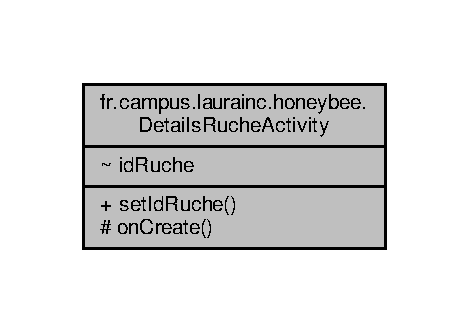
\includegraphics[width=225pt]{classfr_1_1campus_1_1laurainc_1_1honeybee_1_1_details_ruche_activity__coll__graph}
\end{center}
\end{figure}
\subsubsection*{Fonctions membres publiques}
\begin{DoxyCompactItemize}
\item 
void \hyperlink{classfr_1_1campus_1_1laurainc_1_1honeybee_1_1_details_ruche_activity_a3b80f41947ee1ea91f410697e6d93f6a}{set\+Id\+Ruche} (int id\+Ruche)
\end{DoxyCompactItemize}
\subsubsection*{Fonctions membres protégées}
\begin{DoxyCompactItemize}
\item 
void \hyperlink{classfr_1_1campus_1_1laurainc_1_1honeybee_1_1_details_ruche_activity_a025e4e802a728d7bd3e68aa7c0f40a08}{on\+Create} (Bundle saved\+Instance\+State)
\end{DoxyCompactItemize}


\subsubsection{Description détaillée}
\begin{DoxyRefDesc}{A faire}
\item[\hyperlink{todo__todo000001}{A faire}]Renommer cettte classe \end{DoxyRefDesc}


\subsubsection{Documentation des fonctions membres}
\mbox{\Hypertarget{classfr_1_1campus_1_1laurainc_1_1honeybee_1_1_details_ruche_activity_a025e4e802a728d7bd3e68aa7c0f40a08}\label{classfr_1_1campus_1_1laurainc_1_1honeybee_1_1_details_ruche_activity_a025e4e802a728d7bd3e68aa7c0f40a08}} 
\index{fr\+::campus\+::laurainc\+::honeybee\+::\+Details\+Ruche\+Activity@{fr\+::campus\+::laurainc\+::honeybee\+::\+Details\+Ruche\+Activity}!on\+Create@{on\+Create}}
\index{on\+Create@{on\+Create}!fr\+::campus\+::laurainc\+::honeybee\+::\+Details\+Ruche\+Activity@{fr\+::campus\+::laurainc\+::honeybee\+::\+Details\+Ruche\+Activity}}
\paragraph{\texorpdfstring{on\+Create()}{onCreate()}}
{\footnotesize\ttfamily void fr.\+campus.\+laurainc.\+honeybee.\+Details\+Ruche\+Activity.\+on\+Create (\begin{DoxyParamCaption}\item[{Bundle}]{saved\+Instance\+State }\end{DoxyParamCaption})\hspace{0.3cm}{\ttfamily [protected]}}


\begin{DoxyCode}
00017     \{
00018         super.onCreate(savedInstanceState);
00019         setContentView(R.layout.activity\_details);
00020 
00021 
00022     \}
\end{DoxyCode}
\mbox{\Hypertarget{classfr_1_1campus_1_1laurainc_1_1honeybee_1_1_details_ruche_activity_a3b80f41947ee1ea91f410697e6d93f6a}\label{classfr_1_1campus_1_1laurainc_1_1honeybee_1_1_details_ruche_activity_a3b80f41947ee1ea91f410697e6d93f6a}} 
\index{fr\+::campus\+::laurainc\+::honeybee\+::\+Details\+Ruche\+Activity@{fr\+::campus\+::laurainc\+::honeybee\+::\+Details\+Ruche\+Activity}!set\+Id\+Ruche@{set\+Id\+Ruche}}
\index{set\+Id\+Ruche@{set\+Id\+Ruche}!fr\+::campus\+::laurainc\+::honeybee\+::\+Details\+Ruche\+Activity@{fr\+::campus\+::laurainc\+::honeybee\+::\+Details\+Ruche\+Activity}}
\paragraph{\texorpdfstring{set\+Id\+Ruche()}{setIdRuche()}}
{\footnotesize\ttfamily void fr.\+campus.\+laurainc.\+honeybee.\+Details\+Ruche\+Activity.\+set\+Id\+Ruche (\begin{DoxyParamCaption}\item[{int}]{id\+Ruche }\end{DoxyParamCaption})}


\begin{DoxyCode}
00024                                         \{
00025         this.idRuche = idRuche;
00026     \}
\end{DoxyCode}


La documentation de cette classe a été générée à partir du fichier suivant \+:\begin{DoxyCompactItemize}
\item 
\hyperlink{_details_ruche_activity_8java}{Details\+Ruche\+Activity.\+java}\end{DoxyCompactItemize}

\hypertarget{struct_donnees_batterie}{}\subsection{Référence de la structure Donnees\+Batterie}
\label{struct_donnees_batterie}\index{Donnees\+Batterie@{Donnees\+Batterie}}


structure de données pour les mesures de la batterie  




{\ttfamily \#include $<$ruche.\+h$>$}



Graphe de collaboration de Donnees\+Batterie\+:\nopagebreak
\begin{figure}[H]
\begin{center}
\leavevmode
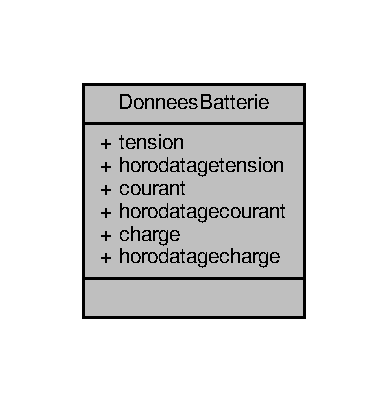
\includegraphics[width=186pt]{struct_donnees_batterie__coll__graph}
\end{center}
\end{figure}
\subsubsection*{Attributs publics}
\begin{DoxyCompactItemize}
\item 
Q\+String \hyperlink{struct_donnees_batterie_a1394510ba159a846820452e9e333f38b}{tension}
\item 
Q\+String \hyperlink{struct_donnees_batterie_ac19dd5bb96d677e228ddd22159076d26}{horodatagetension}
\item 
Q\+String \hyperlink{struct_donnees_batterie_a7a996ea5eacd6839a8a34dbbe48eb59a}{courant}
\item 
Q\+String \hyperlink{struct_donnees_batterie_a1318c296d4e6926304851a7cef0ad957}{horodatagecourant}
\item 
Q\+String \hyperlink{struct_donnees_batterie_a4d3cf76cf1722835a6449bc4a29e761b}{charge}
\item 
Q\+String \hyperlink{struct_donnees_batterie_a98859495d938a84f1c6aa818e0d31e82}{horodatagecharge}
\end{DoxyCompactItemize}


\subsubsection{Description détaillée}
\begin{DoxyAuthor}{Auteur}
Florentin Mellah, Enzo Rossi
\end{DoxyAuthor}
\begin{DoxyVersion}{Version}
1.\+1 
\end{DoxyVersion}


\subsubsection{Documentation des données membres}
\mbox{\Hypertarget{struct_donnees_batterie_a4d3cf76cf1722835a6449bc4a29e761b}\label{struct_donnees_batterie_a4d3cf76cf1722835a6449bc4a29e761b}} 
\index{Donnees\+Batterie@{Donnees\+Batterie}!charge@{charge}}
\index{charge@{charge}!Donnees\+Batterie@{Donnees\+Batterie}}
\paragraph{\texorpdfstring{charge}{charge}}
{\footnotesize\ttfamily Q\+String Donnees\+Batterie\+::charge}



Référencé par \hyperlink{class_ruche_a21c0dafeaec03d451590037343e6a3ca}{Ruche\+::extraire\+Donnees()}, et \hyperlink{class_ruche_a509367d6b2bcb7e6431fc1cc5ff606b5}{Ruche\+::inserer\+Donnees\+Port\+Batterie()}.

\mbox{\Hypertarget{struct_donnees_batterie_a7a996ea5eacd6839a8a34dbbe48eb59a}\label{struct_donnees_batterie_a7a996ea5eacd6839a8a34dbbe48eb59a}} 
\index{Donnees\+Batterie@{Donnees\+Batterie}!courant@{courant}}
\index{courant@{courant}!Donnees\+Batterie@{Donnees\+Batterie}}
\paragraph{\texorpdfstring{courant}{courant}}
{\footnotesize\ttfamily Q\+String Donnees\+Batterie\+::courant}



Référencé par \hyperlink{class_ruche_a21c0dafeaec03d451590037343e6a3ca}{Ruche\+::extraire\+Donnees()}, et \hyperlink{class_ruche_a509367d6b2bcb7e6431fc1cc5ff606b5}{Ruche\+::inserer\+Donnees\+Port\+Batterie()}.

\mbox{\Hypertarget{struct_donnees_batterie_a98859495d938a84f1c6aa818e0d31e82}\label{struct_donnees_batterie_a98859495d938a84f1c6aa818e0d31e82}} 
\index{Donnees\+Batterie@{Donnees\+Batterie}!horodatagecharge@{horodatagecharge}}
\index{horodatagecharge@{horodatagecharge}!Donnees\+Batterie@{Donnees\+Batterie}}
\paragraph{\texorpdfstring{horodatagecharge}{horodatagecharge}}
{\footnotesize\ttfamily Q\+String Donnees\+Batterie\+::horodatagecharge}



Référencé par \hyperlink{class_ruche_a21c0dafeaec03d451590037343e6a3ca}{Ruche\+::extraire\+Donnees()}.

\mbox{\Hypertarget{struct_donnees_batterie_a1318c296d4e6926304851a7cef0ad957}\label{struct_donnees_batterie_a1318c296d4e6926304851a7cef0ad957}} 
\index{Donnees\+Batterie@{Donnees\+Batterie}!horodatagecourant@{horodatagecourant}}
\index{horodatagecourant@{horodatagecourant}!Donnees\+Batterie@{Donnees\+Batterie}}
\paragraph{\texorpdfstring{horodatagecourant}{horodatagecourant}}
{\footnotesize\ttfamily Q\+String Donnees\+Batterie\+::horodatagecourant}



Référencé par \hyperlink{class_ruche_a21c0dafeaec03d451590037343e6a3ca}{Ruche\+::extraire\+Donnees()}.

\mbox{\Hypertarget{struct_donnees_batterie_ac19dd5bb96d677e228ddd22159076d26}\label{struct_donnees_batterie_ac19dd5bb96d677e228ddd22159076d26}} 
\index{Donnees\+Batterie@{Donnees\+Batterie}!horodatagetension@{horodatagetension}}
\index{horodatagetension@{horodatagetension}!Donnees\+Batterie@{Donnees\+Batterie}}
\paragraph{\texorpdfstring{horodatagetension}{horodatagetension}}
{\footnotesize\ttfamily Q\+String Donnees\+Batterie\+::horodatagetension}



Référencé par \hyperlink{class_ruche_a21c0dafeaec03d451590037343e6a3ca}{Ruche\+::extraire\+Donnees()}.

\mbox{\Hypertarget{struct_donnees_batterie_a1394510ba159a846820452e9e333f38b}\label{struct_donnees_batterie_a1394510ba159a846820452e9e333f38b}} 
\index{Donnees\+Batterie@{Donnees\+Batterie}!tension@{tension}}
\index{tension@{tension}!Donnees\+Batterie@{Donnees\+Batterie}}
\paragraph{\texorpdfstring{tension}{tension}}
{\footnotesize\ttfamily Q\+String Donnees\+Batterie\+::tension}



Référencé par \hyperlink{class_ruche_a21c0dafeaec03d451590037343e6a3ca}{Ruche\+::extraire\+Donnees()}, et \hyperlink{class_ruche_a509367d6b2bcb7e6431fc1cc5ff606b5}{Ruche\+::inserer\+Donnees\+Port\+Batterie()}.



La documentation de cette structure a été générée à partir du fichier suivant \+:\begin{DoxyCompactItemize}
\item 
\hyperlink{ruche_8h}{ruche.\+h}\end{DoxyCompactItemize}

\hypertarget{struct_donnees_ruche}{}\subsection{Référence de la structure Donnees\+Ruche}
\label{struct_donnees_ruche}\index{Donnees\+Ruche@{Donnees\+Ruche}}


structure de données pour les mesures horodatées  




{\ttfamily \#include $<$ruche.\+h$>$}



Graphe de collaboration de Donnees\+Ruche\+:\nopagebreak
\begin{figure}[H]
\begin{center}
\leavevmode
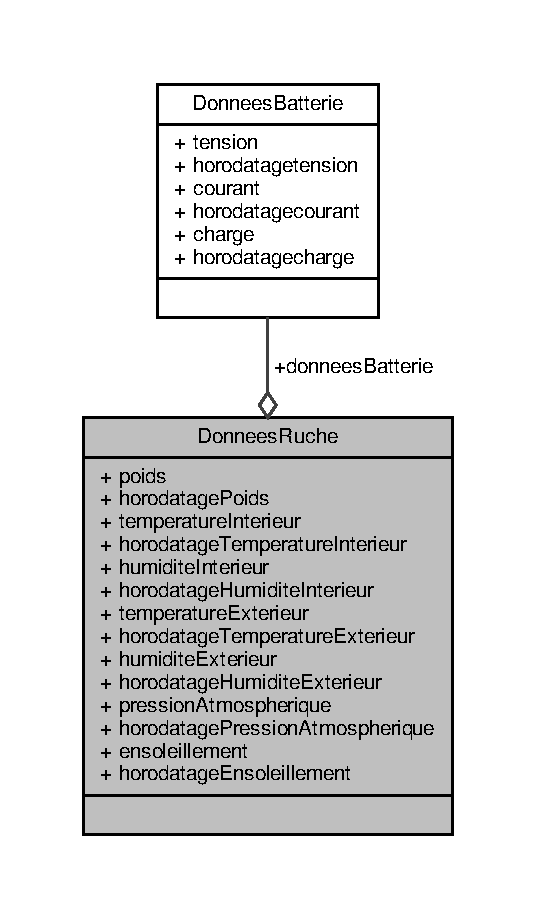
\includegraphics[width=257pt]{struct_donnees_ruche__coll__graph}
\end{center}
\end{figure}
\subsubsection*{Attributs publics}
\begin{DoxyCompactItemize}
\item 
\hyperlink{struct_donnees_batterie}{Donnees\+Batterie} \hyperlink{struct_donnees_ruche_a67dc57b9568529e595a5a31e93eef703}{donnees\+Batterie}
\item 
Q\+String \hyperlink{struct_donnees_ruche_af825ee2a3638e519d531c62311592d20}{poids}
\item 
Q\+String \hyperlink{struct_donnees_ruche_a8f96978c53a79f3c4b450240c67a306d}{horodatage\+Poids}
\item 
Q\+String \hyperlink{struct_donnees_ruche_ad6cbda133d2c8abc23fb688d6e565ab2}{temperature\+Interieur}
\item 
Q\+String \hyperlink{struct_donnees_ruche_a004c7a2447bbcdd2ba212ba2f9866dcd}{horodatage\+Temperature\+Interieur}
\item 
Q\+String \hyperlink{struct_donnees_ruche_a2541ee93816a11da7367b36d4bedc77b}{humidite\+Interieur}
\item 
Q\+String \hyperlink{struct_donnees_ruche_a15ebda778958380edd4acff5d6eef5b8}{horodatage\+Humidite\+Interieur}
\item 
Q\+String \hyperlink{struct_donnees_ruche_aebc52e7707ccf6ae31d2150533cfb0ba}{temperature\+Exterieur}
\item 
Q\+String \hyperlink{struct_donnees_ruche_a91fb0ab596625f4c63fed764dc649dfb}{horodatage\+Temperature\+Exterieur}
\item 
Q\+String \hyperlink{struct_donnees_ruche_ad97156720e4e08cd7aa545cdb8f3822f}{humidite\+Exterieur}
\item 
Q\+String \hyperlink{struct_donnees_ruche_af38a9a06e2f620850ba2d152f189f67b}{horodatage\+Humidite\+Exterieur}
\item 
Q\+String \hyperlink{struct_donnees_ruche_ad34347d2201eeae5834fd5dc4d0ed512}{pression\+Atmospherique}
\item 
Q\+String \hyperlink{struct_donnees_ruche_a21b7eeed18bc28b9c0f19f1ed5da7916}{horodatage\+Pression\+Atmospherique}
\item 
Q\+String \hyperlink{struct_donnees_ruche_adfa6aee15b2a96b968e558ac14e0f2de}{ensoleillement}
\item 
Q\+String \hyperlink{struct_donnees_ruche_ae1b5a2502017455f8fbd95bdab935fd1}{horodatage\+Ensoleillement}
\end{DoxyCompactItemize}


\subsubsection{Description détaillée}
\begin{DoxyAuthor}{Auteur}
Florentin Mellah, Enzo Rossi
\end{DoxyAuthor}
\begin{DoxyVersion}{Version}
1.\+1 
\end{DoxyVersion}


\subsubsection{Documentation des données membres}
\mbox{\Hypertarget{struct_donnees_ruche_a67dc57b9568529e595a5a31e93eef703}\label{struct_donnees_ruche_a67dc57b9568529e595a5a31e93eef703}} 
\index{Donnees\+Ruche@{Donnees\+Ruche}!donnees\+Batterie@{donnees\+Batterie}}
\index{donnees\+Batterie@{donnees\+Batterie}!Donnees\+Ruche@{Donnees\+Ruche}}
\paragraph{\texorpdfstring{donnees\+Batterie}{donneesBatterie}}
{\footnotesize\ttfamily \hyperlink{struct_donnees_batterie}{Donnees\+Batterie} Donnees\+Ruche\+::donnees\+Batterie}



Référencé par \hyperlink{class_ruche_a21c0dafeaec03d451590037343e6a3ca}{Ruche\+::extraire\+Donnees()}, et \hyperlink{class_ruche_a509367d6b2bcb7e6431fc1cc5ff606b5}{Ruche\+::inserer\+Donnees\+Port\+Batterie()}.

\mbox{\Hypertarget{struct_donnees_ruche_adfa6aee15b2a96b968e558ac14e0f2de}\label{struct_donnees_ruche_adfa6aee15b2a96b968e558ac14e0f2de}} 
\index{Donnees\+Ruche@{Donnees\+Ruche}!ensoleillement@{ensoleillement}}
\index{ensoleillement@{ensoleillement}!Donnees\+Ruche@{Donnees\+Ruche}}
\paragraph{\texorpdfstring{ensoleillement}{ensoleillement}}
{\footnotesize\ttfamily Q\+String Donnees\+Ruche\+::ensoleillement}



Référencé par \hyperlink{class_ruche_a21c0dafeaec03d451590037343e6a3ca}{Ruche\+::extraire\+Donnees()}, et \hyperlink{class_ruche_ad21de5f7d48195be0658f52c55f34183}{Ruche\+::inserer\+Donnees\+Port\+Ensoleillement()}.

\mbox{\Hypertarget{struct_donnees_ruche_ae1b5a2502017455f8fbd95bdab935fd1}\label{struct_donnees_ruche_ae1b5a2502017455f8fbd95bdab935fd1}} 
\index{Donnees\+Ruche@{Donnees\+Ruche}!horodatage\+Ensoleillement@{horodatage\+Ensoleillement}}
\index{horodatage\+Ensoleillement@{horodatage\+Ensoleillement}!Donnees\+Ruche@{Donnees\+Ruche}}
\paragraph{\texorpdfstring{horodatage\+Ensoleillement}{horodatageEnsoleillement}}
{\footnotesize\ttfamily Q\+String Donnees\+Ruche\+::horodatage\+Ensoleillement}



Référencé par \hyperlink{class_ruche_a21c0dafeaec03d451590037343e6a3ca}{Ruche\+::extraire\+Donnees()}.

\mbox{\Hypertarget{struct_donnees_ruche_af38a9a06e2f620850ba2d152f189f67b}\label{struct_donnees_ruche_af38a9a06e2f620850ba2d152f189f67b}} 
\index{Donnees\+Ruche@{Donnees\+Ruche}!horodatage\+Humidite\+Exterieur@{horodatage\+Humidite\+Exterieur}}
\index{horodatage\+Humidite\+Exterieur@{horodatage\+Humidite\+Exterieur}!Donnees\+Ruche@{Donnees\+Ruche}}
\paragraph{\texorpdfstring{horodatage\+Humidite\+Exterieur}{horodatageHumiditeExterieur}}
{\footnotesize\ttfamily Q\+String Donnees\+Ruche\+::horodatage\+Humidite\+Exterieur}



Référencé par \hyperlink{class_ruche_a21c0dafeaec03d451590037343e6a3ca}{Ruche\+::extraire\+Donnees()}.

\mbox{\Hypertarget{struct_donnees_ruche_a15ebda778958380edd4acff5d6eef5b8}\label{struct_donnees_ruche_a15ebda778958380edd4acff5d6eef5b8}} 
\index{Donnees\+Ruche@{Donnees\+Ruche}!horodatage\+Humidite\+Interieur@{horodatage\+Humidite\+Interieur}}
\index{horodatage\+Humidite\+Interieur@{horodatage\+Humidite\+Interieur}!Donnees\+Ruche@{Donnees\+Ruche}}
\paragraph{\texorpdfstring{horodatage\+Humidite\+Interieur}{horodatageHumiditeInterieur}}
{\footnotesize\ttfamily Q\+String Donnees\+Ruche\+::horodatage\+Humidite\+Interieur}



Référencé par \hyperlink{class_ruche_a21c0dafeaec03d451590037343e6a3ca}{Ruche\+::extraire\+Donnees()}.

\mbox{\Hypertarget{struct_donnees_ruche_a8f96978c53a79f3c4b450240c67a306d}\label{struct_donnees_ruche_a8f96978c53a79f3c4b450240c67a306d}} 
\index{Donnees\+Ruche@{Donnees\+Ruche}!horodatage\+Poids@{horodatage\+Poids}}
\index{horodatage\+Poids@{horodatage\+Poids}!Donnees\+Ruche@{Donnees\+Ruche}}
\paragraph{\texorpdfstring{horodatage\+Poids}{horodatagePoids}}
{\footnotesize\ttfamily Q\+String Donnees\+Ruche\+::horodatage\+Poids}



Référencé par \hyperlink{class_ruche_a21c0dafeaec03d451590037343e6a3ca}{Ruche\+::extraire\+Donnees()}.

\mbox{\Hypertarget{struct_donnees_ruche_a21b7eeed18bc28b9c0f19f1ed5da7916}\label{struct_donnees_ruche_a21b7eeed18bc28b9c0f19f1ed5da7916}} 
\index{Donnees\+Ruche@{Donnees\+Ruche}!horodatage\+Pression\+Atmospherique@{horodatage\+Pression\+Atmospherique}}
\index{horodatage\+Pression\+Atmospherique@{horodatage\+Pression\+Atmospherique}!Donnees\+Ruche@{Donnees\+Ruche}}
\paragraph{\texorpdfstring{horodatage\+Pression\+Atmospherique}{horodatagePressionAtmospherique}}
{\footnotesize\ttfamily Q\+String Donnees\+Ruche\+::horodatage\+Pression\+Atmospherique}



Référencé par \hyperlink{class_ruche_a21c0dafeaec03d451590037343e6a3ca}{Ruche\+::extraire\+Donnees()}.

\mbox{\Hypertarget{struct_donnees_ruche_a91fb0ab596625f4c63fed764dc649dfb}\label{struct_donnees_ruche_a91fb0ab596625f4c63fed764dc649dfb}} 
\index{Donnees\+Ruche@{Donnees\+Ruche}!horodatage\+Temperature\+Exterieur@{horodatage\+Temperature\+Exterieur}}
\index{horodatage\+Temperature\+Exterieur@{horodatage\+Temperature\+Exterieur}!Donnees\+Ruche@{Donnees\+Ruche}}
\paragraph{\texorpdfstring{horodatage\+Temperature\+Exterieur}{horodatageTemperatureExterieur}}
{\footnotesize\ttfamily Q\+String Donnees\+Ruche\+::horodatage\+Temperature\+Exterieur}



Référencé par \hyperlink{class_ruche_a21c0dafeaec03d451590037343e6a3ca}{Ruche\+::extraire\+Donnees()}.

\mbox{\Hypertarget{struct_donnees_ruche_a004c7a2447bbcdd2ba212ba2f9866dcd}\label{struct_donnees_ruche_a004c7a2447bbcdd2ba212ba2f9866dcd}} 
\index{Donnees\+Ruche@{Donnees\+Ruche}!horodatage\+Temperature\+Interieur@{horodatage\+Temperature\+Interieur}}
\index{horodatage\+Temperature\+Interieur@{horodatage\+Temperature\+Interieur}!Donnees\+Ruche@{Donnees\+Ruche}}
\paragraph{\texorpdfstring{horodatage\+Temperature\+Interieur}{horodatageTemperatureInterieur}}
{\footnotesize\ttfamily Q\+String Donnees\+Ruche\+::horodatage\+Temperature\+Interieur}



Référencé par \hyperlink{class_ruche_a21c0dafeaec03d451590037343e6a3ca}{Ruche\+::extraire\+Donnees()}.

\mbox{\Hypertarget{struct_donnees_ruche_ad97156720e4e08cd7aa545cdb8f3822f}\label{struct_donnees_ruche_ad97156720e4e08cd7aa545cdb8f3822f}} 
\index{Donnees\+Ruche@{Donnees\+Ruche}!humidite\+Exterieur@{humidite\+Exterieur}}
\index{humidite\+Exterieur@{humidite\+Exterieur}!Donnees\+Ruche@{Donnees\+Ruche}}
\paragraph{\texorpdfstring{humidite\+Exterieur}{humiditeExterieur}}
{\footnotesize\ttfamily Q\+String Donnees\+Ruche\+::humidite\+Exterieur}



Référencé par \hyperlink{class_ruche_a21c0dafeaec03d451590037343e6a3ca}{Ruche\+::extraire\+Donnees()}, et \hyperlink{class_ruche_a46c0f440f40a5125f2d579b481660457}{Ruche\+::inserer\+Donnees\+Port\+Mesure\+Environnement()}.

\mbox{\Hypertarget{struct_donnees_ruche_a2541ee93816a11da7367b36d4bedc77b}\label{struct_donnees_ruche_a2541ee93816a11da7367b36d4bedc77b}} 
\index{Donnees\+Ruche@{Donnees\+Ruche}!humidite\+Interieur@{humidite\+Interieur}}
\index{humidite\+Interieur@{humidite\+Interieur}!Donnees\+Ruche@{Donnees\+Ruche}}
\paragraph{\texorpdfstring{humidite\+Interieur}{humiditeInterieur}}
{\footnotesize\ttfamily Q\+String Donnees\+Ruche\+::humidite\+Interieur}



Référencé par \hyperlink{class_ruche_a21c0dafeaec03d451590037343e6a3ca}{Ruche\+::extraire\+Donnees()}, et \hyperlink{class_ruche_aa61f6dd8b15e5242ef3a3bdd87cca4a3}{Ruche\+::inserer\+Donnees\+Port\+Mesure\+Ruche()}.

\mbox{\Hypertarget{struct_donnees_ruche_af825ee2a3638e519d531c62311592d20}\label{struct_donnees_ruche_af825ee2a3638e519d531c62311592d20}} 
\index{Donnees\+Ruche@{Donnees\+Ruche}!poids@{poids}}
\index{poids@{poids}!Donnees\+Ruche@{Donnees\+Ruche}}
\paragraph{\texorpdfstring{poids}{poids}}
{\footnotesize\ttfamily Q\+String Donnees\+Ruche\+::poids}



Référencé par \hyperlink{class_ruche_a21c0dafeaec03d451590037343e6a3ca}{Ruche\+::extraire\+Donnees()}, et \hyperlink{class_ruche_a923f42fc4878a01f6102966a748e8f37}{Ruche\+::inserer\+Donnees\+Port\+Poids()}.

\mbox{\Hypertarget{struct_donnees_ruche_ad34347d2201eeae5834fd5dc4d0ed512}\label{struct_donnees_ruche_ad34347d2201eeae5834fd5dc4d0ed512}} 
\index{Donnees\+Ruche@{Donnees\+Ruche}!pression\+Atmospherique@{pression\+Atmospherique}}
\index{pression\+Atmospherique@{pression\+Atmospherique}!Donnees\+Ruche@{Donnees\+Ruche}}
\paragraph{\texorpdfstring{pression\+Atmospherique}{pressionAtmospherique}}
{\footnotesize\ttfamily Q\+String Donnees\+Ruche\+::pression\+Atmospherique}



Référencé par \hyperlink{class_ruche_a21c0dafeaec03d451590037343e6a3ca}{Ruche\+::extraire\+Donnees()}, et \hyperlink{class_ruche_a46c0f440f40a5125f2d579b481660457}{Ruche\+::inserer\+Donnees\+Port\+Mesure\+Environnement()}.

\mbox{\Hypertarget{struct_donnees_ruche_aebc52e7707ccf6ae31d2150533cfb0ba}\label{struct_donnees_ruche_aebc52e7707ccf6ae31d2150533cfb0ba}} 
\index{Donnees\+Ruche@{Donnees\+Ruche}!temperature\+Exterieur@{temperature\+Exterieur}}
\index{temperature\+Exterieur@{temperature\+Exterieur}!Donnees\+Ruche@{Donnees\+Ruche}}
\paragraph{\texorpdfstring{temperature\+Exterieur}{temperatureExterieur}}
{\footnotesize\ttfamily Q\+String Donnees\+Ruche\+::temperature\+Exterieur}



Référencé par \hyperlink{class_ruche_a21c0dafeaec03d451590037343e6a3ca}{Ruche\+::extraire\+Donnees()}, et \hyperlink{class_ruche_a46c0f440f40a5125f2d579b481660457}{Ruche\+::inserer\+Donnees\+Port\+Mesure\+Environnement()}.

\mbox{\Hypertarget{struct_donnees_ruche_ad6cbda133d2c8abc23fb688d6e565ab2}\label{struct_donnees_ruche_ad6cbda133d2c8abc23fb688d6e565ab2}} 
\index{Donnees\+Ruche@{Donnees\+Ruche}!temperature\+Interieur@{temperature\+Interieur}}
\index{temperature\+Interieur@{temperature\+Interieur}!Donnees\+Ruche@{Donnees\+Ruche}}
\paragraph{\texorpdfstring{temperature\+Interieur}{temperatureInterieur}}
{\footnotesize\ttfamily Q\+String Donnees\+Ruche\+::temperature\+Interieur}



Référencé par \hyperlink{class_ruche_a21c0dafeaec03d451590037343e6a3ca}{Ruche\+::extraire\+Donnees()}, et \hyperlink{class_ruche_aa61f6dd8b15e5242ef3a3bdd87cca4a3}{Ruche\+::inserer\+Donnees\+Port\+Mesure\+Ruche()}.



La documentation de cette structure a été générée à partir du fichier suivant \+:\begin{DoxyCompactItemize}
\item 
\hyperlink{ruche_8h}{ruche.\+h}\end{DoxyCompactItemize}

\hypertarget{classfr_1_1campus_1_1laurainc_1_1honeybee_1_1_example_instrumented_test}{}\subsection{Référence de la classe fr.\+campus.\+laurainc.\+honeybee.\+Example\+Instrumented\+Test}
\label{classfr_1_1campus_1_1laurainc_1_1honeybee_1_1_example_instrumented_test}\index{fr.\+campus.\+laurainc.\+honeybee.\+Example\+Instrumented\+Test@{fr.\+campus.\+laurainc.\+honeybee.\+Example\+Instrumented\+Test}}


Graphe de collaboration de fr.\+campus.\+laurainc.\+honeybee.\+Example\+Instrumented\+Test\+:\nopagebreak
\begin{figure}[H]
\begin{center}
\leavevmode
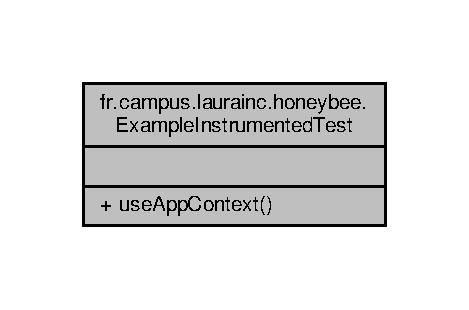
\includegraphics[width=225pt]{classfr_1_1campus_1_1laurainc_1_1honeybee_1_1_example_instrumented_test__coll__graph}
\end{center}
\end{figure}
\subsubsection*{Fonctions membres publiques}
\begin{DoxyCompactItemize}
\item 
void \hyperlink{classfr_1_1campus_1_1laurainc_1_1honeybee_1_1_example_instrumented_test_a9474da2c6615d495569abe302049f465}{use\+App\+Context} ()
\end{DoxyCompactItemize}


\subsubsection{Description détaillée}
Instrumented test, which will execute on an Android device.

\begin{DoxySeeAlso}{Voir également}
\href{http://d.android.com/tools/testing}{\tt Testing documentation} 
\end{DoxySeeAlso}


\subsubsection{Documentation des fonctions membres}
\mbox{\Hypertarget{classfr_1_1campus_1_1laurainc_1_1honeybee_1_1_example_instrumented_test_a9474da2c6615d495569abe302049f465}\label{classfr_1_1campus_1_1laurainc_1_1honeybee_1_1_example_instrumented_test_a9474da2c6615d495569abe302049f465}} 
\index{fr\+::campus\+::laurainc\+::honeybee\+::\+Example\+Instrumented\+Test@{fr\+::campus\+::laurainc\+::honeybee\+::\+Example\+Instrumented\+Test}!use\+App\+Context@{use\+App\+Context}}
\index{use\+App\+Context@{use\+App\+Context}!fr\+::campus\+::laurainc\+::honeybee\+::\+Example\+Instrumented\+Test@{fr\+::campus\+::laurainc\+::honeybee\+::\+Example\+Instrumented\+Test}}
\paragraph{\texorpdfstring{use\+App\+Context()}{useAppContext()}}
{\footnotesize\ttfamily void fr.\+campus.\+laurainc.\+honeybee.\+Example\+Instrumented\+Test.\+use\+App\+Context (\begin{DoxyParamCaption}{ }\end{DoxyParamCaption})}


\begin{DoxyCode}
00020                                 \{
00021         \textcolor{comment}{// Context of the app under test.}
00022         Context appContext = InstrumentationRegistry.getTargetContext();
00023 
00024         assertEquals(\textcolor{stringliteral}{"fr.campus.laurainc.honeybee"}, appContext.getPackageName());
00025     \}
\end{DoxyCode}


La documentation de cette classe a été générée à partir du fichier suivant \+:\begin{DoxyCompactItemize}
\item 
\hyperlink{_example_instrumented_test_8java}{Example\+Instrumented\+Test.\+java}\end{DoxyCompactItemize}

\hypertarget{classfr_1_1campus_1_1laurainc_1_1honeybee_1_1_example_unit_test}{}\subsection{Référence de la classe fr.\+campus.\+laurainc.\+honeybee.\+Example\+Unit\+Test}
\label{classfr_1_1campus_1_1laurainc_1_1honeybee_1_1_example_unit_test}\index{fr.\+campus.\+laurainc.\+honeybee.\+Example\+Unit\+Test@{fr.\+campus.\+laurainc.\+honeybee.\+Example\+Unit\+Test}}


Graphe de collaboration de fr.\+campus.\+laurainc.\+honeybee.\+Example\+Unit\+Test\+:\nopagebreak
\begin{figure}[H]
\begin{center}
\leavevmode
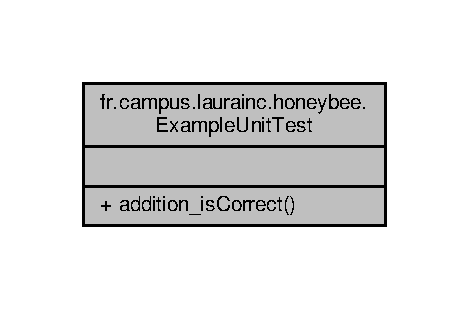
\includegraphics[width=225pt]{classfr_1_1campus_1_1laurainc_1_1honeybee_1_1_example_unit_test__coll__graph}
\end{center}
\end{figure}
\subsubsection*{Fonctions membres publiques}
\begin{DoxyCompactItemize}
\item 
void \hyperlink{classfr_1_1campus_1_1laurainc_1_1honeybee_1_1_example_unit_test_a77a58b717ed25d15b8ed9c20f763ad29}{addition\+\_\+is\+Correct} ()
\end{DoxyCompactItemize}


\subsubsection{Description détaillée}
Example local unit test, which will execute on the development machine (host).

\begin{DoxySeeAlso}{Voir également}
\href{http://d.android.com/tools/testing}{\tt Testing documentation} 
\end{DoxySeeAlso}


\subsubsection{Documentation des fonctions membres}
\mbox{\Hypertarget{classfr_1_1campus_1_1laurainc_1_1honeybee_1_1_example_unit_test_a77a58b717ed25d15b8ed9c20f763ad29}\label{classfr_1_1campus_1_1laurainc_1_1honeybee_1_1_example_unit_test_a77a58b717ed25d15b8ed9c20f763ad29}} 
\index{fr\+::campus\+::laurainc\+::honeybee\+::\+Example\+Unit\+Test@{fr\+::campus\+::laurainc\+::honeybee\+::\+Example\+Unit\+Test}!addition\+\_\+is\+Correct@{addition\+\_\+is\+Correct}}
\index{addition\+\_\+is\+Correct@{addition\+\_\+is\+Correct}!fr\+::campus\+::laurainc\+::honeybee\+::\+Example\+Unit\+Test@{fr\+::campus\+::laurainc\+::honeybee\+::\+Example\+Unit\+Test}}
\paragraph{\texorpdfstring{addition\+\_\+is\+Correct()}{addition\_isCorrect()}}
{\footnotesize\ttfamily void fr.\+campus.\+laurainc.\+honeybee.\+Example\+Unit\+Test.\+addition\+\_\+is\+Correct (\begin{DoxyParamCaption}{ }\end{DoxyParamCaption})}


\begin{DoxyCode}
00014                                      \{
00015         assertEquals(4, 2 + 2);
00016     \}
\end{DoxyCode}


La documentation de cette classe a été générée à partir du fichier suivant \+:\begin{DoxyCompactItemize}
\item 
\hyperlink{_example_unit_test_8java}{Example\+Unit\+Test.\+java}\end{DoxyCompactItemize}

\hypertarget{classfr_1_1campus_1_1laurainc_1_1honeybee_1_1_graph_activity}{}\subsection{Référence de la classe fr.\+campus.\+laurainc.\+honeybee.\+Graph\+Activity}
\label{classfr_1_1campus_1_1laurainc_1_1honeybee_1_1_graph_activity}\index{fr.\+campus.\+laurainc.\+honeybee.\+Graph\+Activity@{fr.\+campus.\+laurainc.\+honeybee.\+Graph\+Activity}}


Graphe de collaboration de fr.\+campus.\+laurainc.\+honeybee.\+Graph\+Activity\+:\nopagebreak
\begin{figure}[H]
\begin{center}
\leavevmode
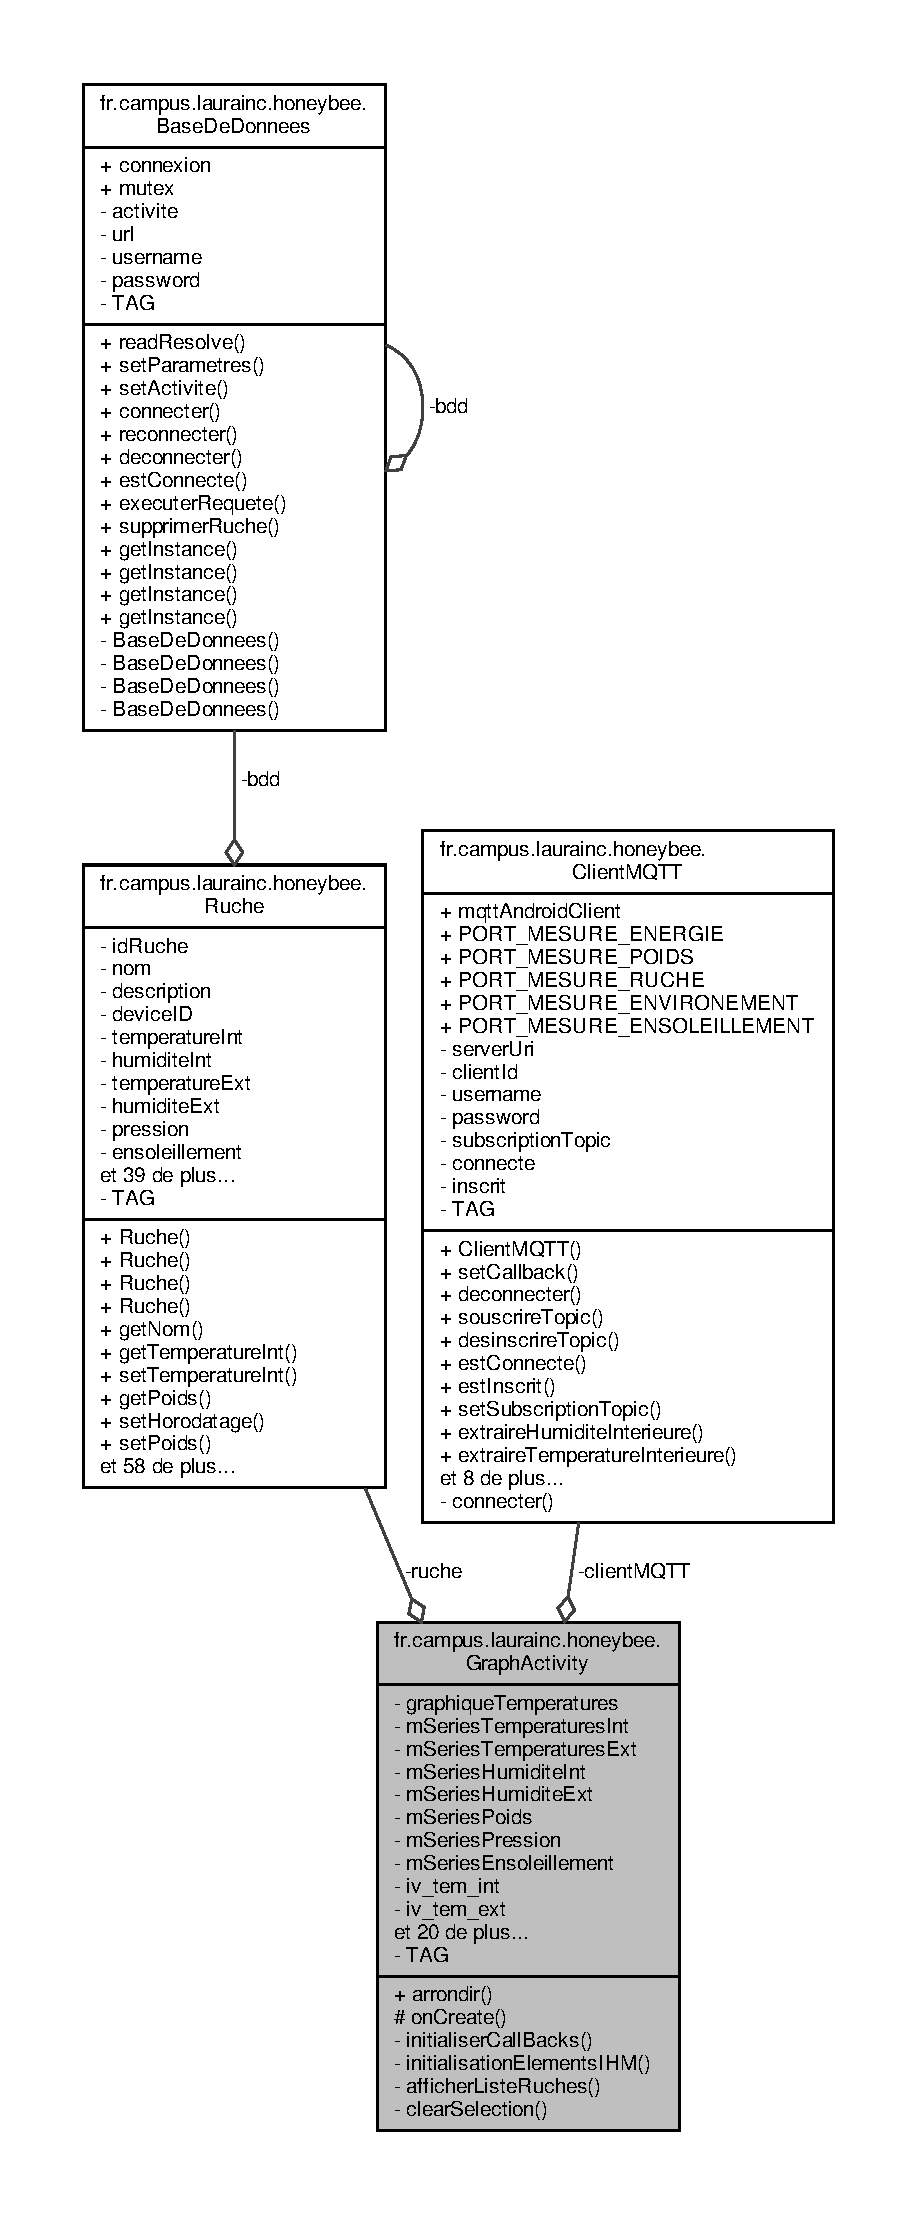
\includegraphics[height=550pt]{classfr_1_1campus_1_1laurainc_1_1honeybee_1_1_graph_activity__coll__graph}
\end{center}
\end{figure}
\subsubsection*{Fonctions membres publiques}
\begin{DoxyCompactItemize}
\item 
double \hyperlink{classfr_1_1campus_1_1laurainc_1_1honeybee_1_1_graph_activity_aaf3c4463ff3eba3ea6e5e2ce28b2c060}{arrondir} (double nombre, double nb\+Apres\+Virgule)
\end{DoxyCompactItemize}
\subsubsection*{Fonctions membres protégées}
\begin{DoxyCompactItemize}
\item 
void \hyperlink{classfr_1_1campus_1_1laurainc_1_1honeybee_1_1_graph_activity_a0a59a4caee62f5c1ce090274c1df66b8}{on\+Create} (Bundle saved\+Instance\+State)
\end{DoxyCompactItemize}
\subsubsection*{Fonctions membres privées}
\begin{DoxyCompactItemize}
\item 
void \hyperlink{classfr_1_1campus_1_1laurainc_1_1honeybee_1_1_graph_activity_a8dc56c3e0744bcb9295ad10e726b5fdb}{initialiser\+Call\+Backs} ()
\item 
void \hyperlink{classfr_1_1campus_1_1laurainc_1_1honeybee_1_1_graph_activity_a7000895983725c6f795f7c73c1fafd20}{initialisation\+Elements\+I\+HM} ()
\item 
void \hyperlink{classfr_1_1campus_1_1laurainc_1_1honeybee_1_1_graph_activity_a9e7c089cbecac26d4251fa5310038107}{afficher\+Liste\+Ruches} ()
\item 
void \hyperlink{classfr_1_1campus_1_1laurainc_1_1honeybee_1_1_graph_activity_a08cfe45ba23b2f1c40e9812bfe1a1f01}{clear\+Selection} ()
\end{DoxyCompactItemize}
\subsubsection*{Attributs privés}
\begin{DoxyCompactItemize}
\item 
\hyperlink{classfr_1_1campus_1_1laurainc_1_1honeybee_1_1_ruche}{Ruche} \hyperlink{classfr_1_1campus_1_1laurainc_1_1honeybee_1_1_graph_activity_ae4312ed40c4a4bf731eb0834155165de}{ruche}
\item 
Graph\+View \hyperlink{classfr_1_1campus_1_1laurainc_1_1honeybee_1_1_graph_activity_ab266262244788c2878b8f1b0587ae5ad}{graphique\+Temperatures}
\item 
Line\+Graph\+Series$<$ Data\+Point $>$ \hyperlink{classfr_1_1campus_1_1laurainc_1_1honeybee_1_1_graph_activity_a0a5faff0e85294ef75aa3b1afb0f8cf2}{m\+Series\+Temperatures\+Int}
\item 
Line\+Graph\+Series$<$ Data\+Point $>$ \hyperlink{classfr_1_1campus_1_1laurainc_1_1honeybee_1_1_graph_activity_ab4e67db85750e356273ec881b5d7849a}{m\+Series\+Temperatures\+Ext}
\item 
Line\+Graph\+Series$<$ Data\+Point $>$ \hyperlink{classfr_1_1campus_1_1laurainc_1_1honeybee_1_1_graph_activity_aebad7eb40c8666969929c1e0255c38b2}{m\+Series\+Humidite\+Int}
\item 
Line\+Graph\+Series$<$ Data\+Point $>$ \hyperlink{classfr_1_1campus_1_1laurainc_1_1honeybee_1_1_graph_activity_a191bf203708992e5708ddfd602d15d7e}{m\+Series\+Humidite\+Ext}
\item 
Line\+Graph\+Series$<$ Data\+Point $>$ \hyperlink{classfr_1_1campus_1_1laurainc_1_1honeybee_1_1_graph_activity_a6287d8e68e9e3f445a1210aaac4fed17}{m\+Series\+Poids}
\item 
Line\+Graph\+Series$<$ Data\+Point $>$ \hyperlink{classfr_1_1campus_1_1laurainc_1_1honeybee_1_1_graph_activity_add9a9c84ba52f748a7dd8c214f2a0484}{m\+Series\+Pression}
\item 
Line\+Graph\+Series$<$ Data\+Point $>$ \hyperlink{classfr_1_1campus_1_1laurainc_1_1honeybee_1_1_graph_activity_aa8c09689c2a865130f123b0b135b669e}{m\+Series\+Ensoleillement}
\item 
Button \hyperlink{classfr_1_1campus_1_1laurainc_1_1honeybee_1_1_graph_activity_a87bc6d987048615fed69785ee38e9b86}{iv\+\_\+tem\+\_\+int}
\item 
Button \hyperlink{classfr_1_1campus_1_1laurainc_1_1honeybee_1_1_graph_activity_a3b757042d1dec4fb097bb37f3a06d516}{iv\+\_\+tem\+\_\+ext}
\item 
Button \hyperlink{classfr_1_1campus_1_1laurainc_1_1honeybee_1_1_graph_activity_a4d73d3543c96bb9b515fa67c8ad786f6}{iv\+\_\+humidite\+\_\+int}
\item 
Button \hyperlink{classfr_1_1campus_1_1laurainc_1_1honeybee_1_1_graph_activity_ac13880806c185e24ce2818072485141c}{iv\+\_\+humidite\+\_\+ext}
\item 
Button \hyperlink{classfr_1_1campus_1_1laurainc_1_1honeybee_1_1_graph_activity_a0508cfebc83dee33b08796d173b0a9d9}{iv\+\_\+poids}
\item 
Button \hyperlink{classfr_1_1campus_1_1laurainc_1_1honeybee_1_1_graph_activity_a4933271aee8d05223844deaf73ee1802}{iv\+\_\+ensoleillement}
\item 
Button \hyperlink{classfr_1_1campus_1_1laurainc_1_1honeybee_1_1_graph_activity_adceab844bbd8bf97865edff454b989de}{iv\+\_\+pression}
\item 
boolean \hyperlink{classfr_1_1campus_1_1laurainc_1_1honeybee_1_1_graph_activity_a42b3b24902493985e648cb0147d93c22}{temp\+\_\+int\+\_\+afficher}
\item 
boolean \hyperlink{classfr_1_1campus_1_1laurainc_1_1honeybee_1_1_graph_activity_aec5260a49cf7ae916c0ac7c1ef9a6689}{temp\+\_\+ext\+\_\+afficher}
\item 
boolean \hyperlink{classfr_1_1campus_1_1laurainc_1_1honeybee_1_1_graph_activity_a0ffe83f5abece5283d33075072dcd168}{humidite\+\_\+int\+\_\+afficher}
\item 
boolean \hyperlink{classfr_1_1campus_1_1laurainc_1_1honeybee_1_1_graph_activity_a10989d0e408b0bb4c2a337172e170c33}{humidite\+\_\+ext\+\_\+afficher}
\item 
boolean \hyperlink{classfr_1_1campus_1_1laurainc_1_1honeybee_1_1_graph_activity_a520066e32b93800ff78699cb5b6cfb60}{poids\+\_\+afficher}
\item 
boolean \hyperlink{classfr_1_1campus_1_1laurainc_1_1honeybee_1_1_graph_activity_a624363bfa1459b895626db0fa31ed6d6}{ensoleillement\+\_\+afficher}
\item 
boolean \hyperlink{classfr_1_1campus_1_1laurainc_1_1honeybee_1_1_graph_activity_ab622b597710c1ff074ed7bf633ce2757}{pression\+\_\+afficher}
\item 
boolean \hyperlink{classfr_1_1campus_1_1laurainc_1_1honeybee_1_1_graph_activity_ac6eaba0cf31484d2b5c63f6fb6bf9320}{temps\+\_\+reel\+\_\+afficher}
\item 
\hyperlink{classfr_1_1campus_1_1laurainc_1_1honeybee_1_1_client_m_q_t_t}{Client\+M\+Q\+TT} \hyperlink{classfr_1_1campus_1_1laurainc_1_1honeybee_1_1_graph_activity_acca0959cd97f62f9b106e714eb4bff5a}{client\+M\+Q\+TT}
\item 
Text\+View \hyperlink{classfr_1_1campus_1_1laurainc_1_1honeybee_1_1_graph_activity_a32402fa5819cf8f4322c3ae033a3c001}{tv\+\_\+valeur\+Courante}
\item 
Text\+View \hyperlink{classfr_1_1campus_1_1laurainc_1_1honeybee_1_1_graph_activity_a45953a1c53190ccbf5278e9725a2ce43}{tv\+\_\+donnees\+Bas}
\item 
Text\+View \hyperlink{classfr_1_1campus_1_1laurainc_1_1honeybee_1_1_graph_activity_a13bbba64ced68ea5c90d2761aaa70ac7}{tv\+\_\+donnees\+Moyenne}
\item 
Text\+View \hyperlink{classfr_1_1campus_1_1laurainc_1_1honeybee_1_1_graph_activity_afd8484aa261322b9c4df52fcfc69b1ac}{tv\+\_\+donnees\+Haut}
\item 
Spinner \hyperlink{classfr_1_1campus_1_1laurainc_1_1honeybee_1_1_graph_activity_ad937ed762b691b70747bb9f0b4d44994}{choix\+Ruche}
\item 
Array\+List$<$ String $>$ \hyperlink{classfr_1_1campus_1_1laurainc_1_1honeybee_1_1_graph_activity_ac3cf2f6b767bd189dc5c85ecbb48d0f6}{mes\+Ruches}
\item 
final Handler \hyperlink{classfr_1_1campus_1_1laurainc_1_1honeybee_1_1_graph_activity_ac42217c5db8be9ce814ab813e2d3080c}{handler}
\end{DoxyCompactItemize}
\subsubsection*{Attributs privés statiques}
\begin{DoxyCompactItemize}
\item 
static final String \hyperlink{classfr_1_1campus_1_1laurainc_1_1honeybee_1_1_graph_activity_a23295afaba61fcec14a254a6359deea4}{T\+AG} = \char`\"{}Graph\+Activity\char`\"{}
\end{DoxyCompactItemize}


\subsubsection{Documentation des fonctions membres}
\mbox{\Hypertarget{classfr_1_1campus_1_1laurainc_1_1honeybee_1_1_graph_activity_a9e7c089cbecac26d4251fa5310038107}\label{classfr_1_1campus_1_1laurainc_1_1honeybee_1_1_graph_activity_a9e7c089cbecac26d4251fa5310038107}} 
\index{fr\+::campus\+::laurainc\+::honeybee\+::\+Graph\+Activity@{fr\+::campus\+::laurainc\+::honeybee\+::\+Graph\+Activity}!afficher\+Liste\+Ruches@{afficher\+Liste\+Ruches}}
\index{afficher\+Liste\+Ruches@{afficher\+Liste\+Ruches}!fr\+::campus\+::laurainc\+::honeybee\+::\+Graph\+Activity@{fr\+::campus\+::laurainc\+::honeybee\+::\+Graph\+Activity}}
\paragraph{\texorpdfstring{afficher\+Liste\+Ruches()}{afficherListeRuches()}}
{\footnotesize\ttfamily void fr.\+campus.\+laurainc.\+honeybee.\+Graph\+Activity.\+afficher\+Liste\+Ruches (\begin{DoxyParamCaption}{ }\end{DoxyParamCaption})\hspace{0.3cm}{\ttfamily [private]}}



Références \hyperlink{classfr_1_1campus_1_1laurainc_1_1honeybee_1_1_ruche_a7108fb412c0628d3966aa8c76fd9e2b7}{fr.\+campus.\+laurainc.\+honeybee.\+Ruche.\+get\+Liste\+Ruches()}, \hyperlink{classfr_1_1campus_1_1laurainc_1_1honeybee_1_1_graph_activity_ac42217c5db8be9ce814ab813e2d3080c}{fr.\+campus.\+laurainc.\+honeybee.\+Graph\+Activity.\+handler}, et \hyperlink{classfr_1_1campus_1_1laurainc_1_1honeybee_1_1_graph_activity_ac3cf2f6b767bd189dc5c85ecbb48d0f6}{fr.\+campus.\+laurainc.\+honeybee.\+Graph\+Activity.\+mes\+Ruches}.


\begin{DoxyCode}
00347                                        \{
00348         \hyperlink{classfr_1_1campus_1_1laurainc_1_1honeybee_1_1_graph_activity_ac3cf2f6b767bd189dc5c85ecbb48d0f6}{mesRuches} = \hyperlink{classfr_1_1campus_1_1laurainc_1_1honeybee_1_1_graph_activity_ae4312ed40c4a4bf731eb0834155165de}{ruche}.\hyperlink{classfr_1_1campus_1_1laurainc_1_1honeybee_1_1_ruche_a7108fb412c0628d3966aa8c76fd9e2b7}{getListeRuches}();
00349         ArrayAdapter<String> adapter = \textcolor{keyword}{new} ArrayAdapter<String>(\textcolor{keyword}{this}, R.layout.item\_spinner ,
      \hyperlink{classfr_1_1campus_1_1laurainc_1_1honeybee_1_1_graph_activity_ac3cf2f6b767bd189dc5c85ecbb48d0f6}{mesRuches});
00350         adapter.setDropDownViewResource(android.R.layout.simple\_spinner\_dropdown\_item);
00351         \hyperlink{classfr_1_1campus_1_1laurainc_1_1honeybee_1_1_graph_activity_ad937ed762b691b70747bb9f0b4d44994}{choixRuche}.setAdapter(adapter);
00352         \hyperlink{classfr_1_1campus_1_1laurainc_1_1honeybee_1_1_graph_activity_ad937ed762b691b70747bb9f0b4d44994}{choixRuche}.setSelection(0);
00353         \textcolor{comment}{//adapter.setNotifyOnChange(true);}
00354 
00355         \hyperlink{classfr_1_1campus_1_1laurainc_1_1honeybee_1_1_graph_activity_ad937ed762b691b70747bb9f0b4d44994}{choixRuche}.setOnItemSelectedListener(\textcolor{keyword}{new} AdapterView.OnItemSelectedListener()
00356         \{
00357             @Override
00358             \textcolor{keyword}{public} \textcolor{keywordtype}{void} onItemSelected(AdapterView<?> arg0, View arg1, \textcolor{keywordtype}{int} position, \textcolor{keywordtype}{long} \textcolor{keywordtype}{id})
00359             \{
00360                 Toast.makeText(getBaseContext(), \hyperlink{classfr_1_1campus_1_1laurainc_1_1honeybee_1_1_graph_activity_ac3cf2f6b767bd189dc5c85ecbb48d0f6}{mesRuches}.get(position), Toast.LENGTH\_SHORT).show
      ();
00361                 Log.d(\hyperlink{classfr_1_1campus_1_1laurainc_1_1honeybee_1_1_graph_activity_a23295afaba61fcec14a254a6359deea4}{TAG}, \textcolor{stringliteral}{"position : "} + position);
00362                 \textcolor{comment}{/*if(clientMQTT != null)
}
00363 \textcolor{comment}{                \{
}
00364 \textcolor{comment}{                    if(clientMQTT.estConnecte())
}
00365 \textcolor{comment}{                        clientMQTT.deconnecter();
}
00366 \textcolor{comment}{}
00367 \textcolor{comment}{                \}*/}
00368                 \textcolor{comment}{// Instancie une ruche}
00369                 \hyperlink{classfr_1_1campus_1_1laurainc_1_1honeybee_1_1_graph_activity_ae4312ed40c4a4bf731eb0834155165de}{ruche} = \textcolor{keyword}{new} \hyperlink{class_ruche}{Ruche}(\hyperlink{classfr_1_1campus_1_1laurainc_1_1honeybee_1_1_graph_activity_ac3cf2f6b767bd189dc5c85ecbb48d0f6}{mesRuches}.get(position), 
      \hyperlink{classfr_1_1campus_1_1laurainc_1_1honeybee_1_1_graph_activity_ac42217c5db8be9ce814ab813e2d3080c}{handler});
00370             \}
00371 
00372             @Override
00373             \textcolor{keyword}{public} \textcolor{keywordtype}{void} onNothingSelected(AdapterView<?> arg0)
00374             \{
00375                 \textcolor{comment}{// TODO Auto-generated method stub}
00376             \}
00377         \});
00378     \}
\end{DoxyCode}
\mbox{\Hypertarget{classfr_1_1campus_1_1laurainc_1_1honeybee_1_1_graph_activity_aaf3c4463ff3eba3ea6e5e2ce28b2c060}\label{classfr_1_1campus_1_1laurainc_1_1honeybee_1_1_graph_activity_aaf3c4463ff3eba3ea6e5e2ce28b2c060}} 
\index{fr\+::campus\+::laurainc\+::honeybee\+::\+Graph\+Activity@{fr\+::campus\+::laurainc\+::honeybee\+::\+Graph\+Activity}!arrondir@{arrondir}}
\index{arrondir@{arrondir}!fr\+::campus\+::laurainc\+::honeybee\+::\+Graph\+Activity@{fr\+::campus\+::laurainc\+::honeybee\+::\+Graph\+Activity}}
\paragraph{\texorpdfstring{arrondir()}{arrondir()}}
{\footnotesize\ttfamily double fr.\+campus.\+laurainc.\+honeybee.\+Graph\+Activity.\+arrondir (\begin{DoxyParamCaption}\item[{double}]{nombre,  }\item[{double}]{nb\+Apres\+Virgule }\end{DoxyParamCaption})}


\begin{DoxyCode}
00408     \{
00409         \textcolor{keywordflow}{return}(\textcolor{keywordtype}{double})((int)(nombre * Math.pow(10,nbApresVirgule) + .5)) / Math.pow(10,nbApresVirgule);
00410     \}
\end{DoxyCode}
\mbox{\Hypertarget{classfr_1_1campus_1_1laurainc_1_1honeybee_1_1_graph_activity_a08cfe45ba23b2f1c40e9812bfe1a1f01}\label{classfr_1_1campus_1_1laurainc_1_1honeybee_1_1_graph_activity_a08cfe45ba23b2f1c40e9812bfe1a1f01}} 
\index{fr\+::campus\+::laurainc\+::honeybee\+::\+Graph\+Activity@{fr\+::campus\+::laurainc\+::honeybee\+::\+Graph\+Activity}!clear\+Selection@{clear\+Selection}}
\index{clear\+Selection@{clear\+Selection}!fr\+::campus\+::laurainc\+::honeybee\+::\+Graph\+Activity@{fr\+::campus\+::laurainc\+::honeybee\+::\+Graph\+Activity}}
\paragraph{\texorpdfstring{clear\+Selection()}{clearSelection()}}
{\footnotesize\ttfamily void fr.\+campus.\+laurainc.\+honeybee.\+Graph\+Activity.\+clear\+Selection (\begin{DoxyParamCaption}{ }\end{DoxyParamCaption})\hspace{0.3cm}{\ttfamily [private]}}



Référencé par \hyperlink{classfr_1_1campus_1_1laurainc_1_1honeybee_1_1_graph_activity_a8dc56c3e0744bcb9295ad10e726b5fdb}{fr.\+campus.\+laurainc.\+honeybee.\+Graph\+Activity.\+initialiser\+Call\+Backs()}.


\begin{DoxyCode}
00381     \{
00382         \hyperlink{classfr_1_1campus_1_1laurainc_1_1honeybee_1_1_graph_activity_a3b757042d1dec4fb097bb37f3a06d516}{iv\_tem\_ext}.setBackgroundResource(0);
00383         \hyperlink{classfr_1_1campus_1_1laurainc_1_1honeybee_1_1_graph_activity_aec5260a49cf7ae916c0ac7c1ef9a6689}{temp\_ext\_afficher} = \textcolor{keyword}{false};
00384 
00385         \hyperlink{classfr_1_1campus_1_1laurainc_1_1honeybee_1_1_graph_activity_a87bc6d987048615fed69785ee38e9b86}{iv\_tem\_int}.setBackgroundResource(0);
00386         \hyperlink{classfr_1_1campus_1_1laurainc_1_1honeybee_1_1_graph_activity_a42b3b24902493985e648cb0147d93c22}{temp\_int\_afficher} = \textcolor{keyword}{false};
00387 
00388         \hyperlink{classfr_1_1campus_1_1laurainc_1_1honeybee_1_1_graph_activity_a4d73d3543c96bb9b515fa67c8ad786f6}{iv\_humidite\_int}.setBackgroundResource(0);
00389         \hyperlink{classfr_1_1campus_1_1laurainc_1_1honeybee_1_1_graph_activity_a0ffe83f5abece5283d33075072dcd168}{humidite\_int\_afficher} = \textcolor{keyword}{false};
00390 
00391         \hyperlink{classfr_1_1campus_1_1laurainc_1_1honeybee_1_1_graph_activity_ac13880806c185e24ce2818072485141c}{iv\_humidite\_ext}.setBackgroundResource(0);
00392         \hyperlink{classfr_1_1campus_1_1laurainc_1_1honeybee_1_1_graph_activity_a10989d0e408b0bb4c2a337172e170c33}{humidite\_ext\_afficher} = \textcolor{keyword}{false};
00393 
00394         \hyperlink{classfr_1_1campus_1_1laurainc_1_1honeybee_1_1_graph_activity_a0508cfebc83dee33b08796d173b0a9d9}{iv\_poids}.setBackgroundResource(0);
00395         \hyperlink{classfr_1_1campus_1_1laurainc_1_1honeybee_1_1_graph_activity_a520066e32b93800ff78699cb5b6cfb60}{poids\_afficher} = \textcolor{keyword}{false};
00396 
00397         \hyperlink{classfr_1_1campus_1_1laurainc_1_1honeybee_1_1_graph_activity_adceab844bbd8bf97865edff454b989de}{iv\_pression}.setBackgroundResource(0);
00398         \hyperlink{classfr_1_1campus_1_1laurainc_1_1honeybee_1_1_graph_activity_ab622b597710c1ff074ed7bf633ce2757}{pression\_afficher} = \textcolor{keyword}{false};
00399 
00400         \hyperlink{classfr_1_1campus_1_1laurainc_1_1honeybee_1_1_graph_activity_a4933271aee8d05223844deaf73ee1802}{iv\_ensoleillement}.setBackgroundResource(0);
00401         \hyperlink{classfr_1_1campus_1_1laurainc_1_1honeybee_1_1_graph_activity_a624363bfa1459b895626db0fa31ed6d6}{ensoleillement\_afficher} = \textcolor{keyword}{false};
00402 
00403         \hyperlink{classfr_1_1campus_1_1laurainc_1_1honeybee_1_1_graph_activity_ab266262244788c2878b8f1b0587ae5ad}{graphiqueTemperatures}.removeAllSeries();
00404 
00405     \}
\end{DoxyCode}
\mbox{\Hypertarget{classfr_1_1campus_1_1laurainc_1_1honeybee_1_1_graph_activity_a7000895983725c6f795f7c73c1fafd20}\label{classfr_1_1campus_1_1laurainc_1_1honeybee_1_1_graph_activity_a7000895983725c6f795f7c73c1fafd20}} 
\index{fr\+::campus\+::laurainc\+::honeybee\+::\+Graph\+Activity@{fr\+::campus\+::laurainc\+::honeybee\+::\+Graph\+Activity}!initialisation\+Elements\+I\+HM@{initialisation\+Elements\+I\+HM}}
\index{initialisation\+Elements\+I\+HM@{initialisation\+Elements\+I\+HM}!fr\+::campus\+::laurainc\+::honeybee\+::\+Graph\+Activity@{fr\+::campus\+::laurainc\+::honeybee\+::\+Graph\+Activity}}
\paragraph{\texorpdfstring{initialisation\+Elements\+I\+H\+M()}{initialisationElementsIHM()}}
{\footnotesize\ttfamily void fr.\+campus.\+laurainc.\+honeybee.\+Graph\+Activity.\+initialisation\+Elements\+I\+HM (\begin{DoxyParamCaption}{ }\end{DoxyParamCaption})\hspace{0.3cm}{\ttfamily [private]}}



Références \hyperlink{classfr_1_1campus_1_1laurainc_1_1honeybee_1_1_ruche_afb6dfa76b8c8c35151face6a5fe32044}{fr.\+campus.\+laurainc.\+honeybee.\+Ruche.\+getm\+Series\+Ensoleillement()}, \hyperlink{classfr_1_1campus_1_1laurainc_1_1honeybee_1_1_ruche_ad1868fa7a9c8f7840e224b06eb03dac9}{fr.\+campus.\+laurainc.\+honeybee.\+Ruche.\+getm\+Series\+Humidite\+Ext()}, \hyperlink{classfr_1_1campus_1_1laurainc_1_1honeybee_1_1_ruche_a2b57090da3912989bbfcc04a76f9e651}{fr.\+campus.\+laurainc.\+honeybee.\+Ruche.\+getm\+Series\+Humidite\+Int()}, \hyperlink{classfr_1_1campus_1_1laurainc_1_1honeybee_1_1_ruche_aebd7c24cbb596731671db1a9554c8351}{fr.\+campus.\+laurainc.\+honeybee.\+Ruche.\+getm\+Series\+Poids()}, \hyperlink{classfr_1_1campus_1_1laurainc_1_1honeybee_1_1_ruche_a237f9b18ebb70839382bc2bfc237b5da}{fr.\+campus.\+laurainc.\+honeybee.\+Ruche.\+getm\+Series\+Pression()}, \hyperlink{classfr_1_1campus_1_1laurainc_1_1honeybee_1_1_ruche_ace771aab9a10f7cf13050197a85c41f7}{fr.\+campus.\+laurainc.\+honeybee.\+Ruche.\+getm\+Series\+Temperatures\+Ext()}, et \hyperlink{classfr_1_1campus_1_1laurainc_1_1honeybee_1_1_ruche_ae3f7d6c16444905061f13fe14eb21d69}{fr.\+campus.\+laurainc.\+honeybee.\+Ruche.\+getm\+Series\+Temperatures\+Int()}.


\begin{DoxyCode}
00302     \{
00303         \hyperlink{classfr_1_1campus_1_1laurainc_1_1honeybee_1_1_graph_activity_a87bc6d987048615fed69785ee38e9b86}{iv\_tem\_int} = findViewById(R.id.btn\_temp\_int);
00304         \hyperlink{classfr_1_1campus_1_1laurainc_1_1honeybee_1_1_graph_activity_a3b757042d1dec4fb097bb37f3a06d516}{iv\_tem\_ext} = findViewById(R.id.btn\_temp\_ext);
00305         \hyperlink{classfr_1_1campus_1_1laurainc_1_1honeybee_1_1_graph_activity_a4d73d3543c96bb9b515fa67c8ad786f6}{iv\_humidite\_int} = findViewById(R.id.btn\_humidite\_int);
00306         \hyperlink{classfr_1_1campus_1_1laurainc_1_1honeybee_1_1_graph_activity_ac13880806c185e24ce2818072485141c}{iv\_humidite\_ext} = findViewById(R.id.btn\_humidite\_ext);
00307         \hyperlink{classfr_1_1campus_1_1laurainc_1_1honeybee_1_1_graph_activity_a0508cfebc83dee33b08796d173b0a9d9}{iv\_poids} = findViewById(R.id.btn\_poids);
00308         \hyperlink{classfr_1_1campus_1_1laurainc_1_1honeybee_1_1_graph_activity_a4933271aee8d05223844deaf73ee1802}{iv\_ensoleillement} = findViewById(R.id.btn\_ensoleillement);
00309         \hyperlink{classfr_1_1campus_1_1laurainc_1_1honeybee_1_1_graph_activity_adceab844bbd8bf97865edff454b989de}{iv\_pression} = findViewById(R.id.btn\_pression);
00310         \hyperlink{classfr_1_1campus_1_1laurainc_1_1honeybee_1_1_graph_activity_a32402fa5819cf8f4322c3ae033a3c001}{tv\_valeurCourante} = findViewById(R.id.tv\_valeurCourante);
00311         \hyperlink{classfr_1_1campus_1_1laurainc_1_1honeybee_1_1_graph_activity_a45953a1c53190ccbf5278e9725a2ce43}{tv\_donneesBas} = findViewById(R.id.tv\_donneesBas);
00312         \hyperlink{classfr_1_1campus_1_1laurainc_1_1honeybee_1_1_graph_activity_a13bbba64ced68ea5c90d2761aaa70ac7}{tv\_donneesMoyenne} = findViewById(R.id.tv\_donneesMoyenne);
00313         \hyperlink{classfr_1_1campus_1_1laurainc_1_1honeybee_1_1_graph_activity_afd8484aa261322b9c4df52fcfc69b1ac}{tv\_donneesHaut} = findViewById(R.id.tv\_donneesHaut);
00314         \textcolor{comment}{//iv\_temps\_reel = findViewById(R.id.iv\_temp\_reel);}
00315 
00316         \hyperlink{classfr_1_1campus_1_1laurainc_1_1honeybee_1_1_graph_activity_a42b3b24902493985e648cb0147d93c22}{temp\_int\_afficher} = \textcolor{keyword}{true};
00317         \hyperlink{classfr_1_1campus_1_1laurainc_1_1honeybee_1_1_graph_activity_aec5260a49cf7ae916c0ac7c1ef9a6689}{temp\_ext\_afficher} = \textcolor{keyword}{false};
00318         \hyperlink{classfr_1_1campus_1_1laurainc_1_1honeybee_1_1_graph_activity_a0ffe83f5abece5283d33075072dcd168}{humidite\_int\_afficher} = \textcolor{keyword}{false};
00319         \hyperlink{classfr_1_1campus_1_1laurainc_1_1honeybee_1_1_graph_activity_a10989d0e408b0bb4c2a337172e170c33}{humidite\_ext\_afficher} = \textcolor{keyword}{false};
00320         \hyperlink{classfr_1_1campus_1_1laurainc_1_1honeybee_1_1_graph_activity_a520066e32b93800ff78699cb5b6cfb60}{poids\_afficher} = \textcolor{keyword}{false};
00321         \hyperlink{classfr_1_1campus_1_1laurainc_1_1honeybee_1_1_graph_activity_a624363bfa1459b895626db0fa31ed6d6}{ensoleillement\_afficher} = \textcolor{keyword}{false};
00322         \hyperlink{classfr_1_1campus_1_1laurainc_1_1honeybee_1_1_graph_activity_ab622b597710c1ff074ed7bf633ce2757}{pression\_afficher} = \textcolor{keyword}{false};
00323         \hyperlink{classfr_1_1campus_1_1laurainc_1_1honeybee_1_1_graph_activity_ac6eaba0cf31484d2b5c63f6fb6bf9320}{temps\_reel\_afficher} = \textcolor{keyword}{false};
00324 
00325         \hyperlink{classfr_1_1campus_1_1laurainc_1_1honeybee_1_1_graph_activity_a0a5faff0e85294ef75aa3b1afb0f8cf2}{mSeriesTemperaturesInt} = \hyperlink{classfr_1_1campus_1_1laurainc_1_1honeybee_1_1_graph_activity_ae4312ed40c4a4bf731eb0834155165de}{ruche}.
      \hyperlink{classfr_1_1campus_1_1laurainc_1_1honeybee_1_1_ruche_ae3f7d6c16444905061f13fe14eb21d69}{getmSeriesTemperaturesInt}();
00326         \hyperlink{classfr_1_1campus_1_1laurainc_1_1honeybee_1_1_graph_activity_ab266262244788c2878b8f1b0587ae5ad}{graphiqueTemperatures}.getViewport().setMaxY(40);
00327         \hyperlink{classfr_1_1campus_1_1laurainc_1_1honeybee_1_1_graph_activity_ab266262244788c2878b8f1b0587ae5ad}{graphiqueTemperatures}.getGridLabelRenderer().setNumVerticalLabels(5);
00328         \hyperlink{classfr_1_1campus_1_1laurainc_1_1honeybee_1_1_graph_activity_ab266262244788c2878b8f1b0587ae5ad}{graphiqueTemperatures}.removeAllSeries();
00329         \hyperlink{classfr_1_1campus_1_1laurainc_1_1honeybee_1_1_graph_activity_ab266262244788c2878b8f1b0587ae5ad}{graphiqueTemperatures}.addSeries(
      \hyperlink{classfr_1_1campus_1_1laurainc_1_1honeybee_1_1_graph_activity_a0a5faff0e85294ef75aa3b1afb0f8cf2}{mSeriesTemperaturesInt});
00330         \hyperlink{classfr_1_1campus_1_1laurainc_1_1honeybee_1_1_graph_activity_ab4e67db85750e356273ec881b5d7849a}{mSeriesTemperaturesExt} = \hyperlink{classfr_1_1campus_1_1laurainc_1_1honeybee_1_1_graph_activity_ae4312ed40c4a4bf731eb0834155165de}{ruche}.
      \hyperlink{classfr_1_1campus_1_1laurainc_1_1honeybee_1_1_ruche_ace771aab9a10f7cf13050197a85c41f7}{getmSeriesTemperaturesExt}();
00331         \hyperlink{classfr_1_1campus_1_1laurainc_1_1honeybee_1_1_graph_activity_aebad7eb40c8666969929c1e0255c38b2}{mSeriesHumiditeInt} = \hyperlink{classfr_1_1campus_1_1laurainc_1_1honeybee_1_1_graph_activity_ae4312ed40c4a4bf731eb0834155165de}{ruche}.\hyperlink{classfr_1_1campus_1_1laurainc_1_1honeybee_1_1_ruche_a2b57090da3912989bbfcc04a76f9e651}{getmSeriesHumiditeInt}();
00332         \hyperlink{classfr_1_1campus_1_1laurainc_1_1honeybee_1_1_graph_activity_a191bf203708992e5708ddfd602d15d7e}{mSeriesHumiditeExt} = \hyperlink{classfr_1_1campus_1_1laurainc_1_1honeybee_1_1_graph_activity_ae4312ed40c4a4bf731eb0834155165de}{ruche}.\hyperlink{classfr_1_1campus_1_1laurainc_1_1honeybee_1_1_ruche_ad1868fa7a9c8f7840e224b06eb03dac9}{getmSeriesHumiditeExt}();
00333         \hyperlink{classfr_1_1campus_1_1laurainc_1_1honeybee_1_1_graph_activity_a6287d8e68e9e3f445a1210aaac4fed17}{mSeriesPoids} = \hyperlink{classfr_1_1campus_1_1laurainc_1_1honeybee_1_1_graph_activity_ae4312ed40c4a4bf731eb0834155165de}{ruche}.\hyperlink{classfr_1_1campus_1_1laurainc_1_1honeybee_1_1_ruche_aebd7c24cbb596731671db1a9554c8351}{getmSeriesPoids}();
00334         \hyperlink{classfr_1_1campus_1_1laurainc_1_1honeybee_1_1_graph_activity_aa8c09689c2a865130f123b0b135b669e}{mSeriesEnsoleillement} = \hyperlink{classfr_1_1campus_1_1laurainc_1_1honeybee_1_1_graph_activity_ae4312ed40c4a4bf731eb0834155165de}{ruche}.
      \hyperlink{classfr_1_1campus_1_1laurainc_1_1honeybee_1_1_ruche_afb6dfa76b8c8c35151face6a5fe32044}{getmSeriesEnsoleillement}();
00335         \hyperlink{classfr_1_1campus_1_1laurainc_1_1honeybee_1_1_graph_activity_add9a9c84ba52f748a7dd8c214f2a0484}{mSeriesPression} = \hyperlink{classfr_1_1campus_1_1laurainc_1_1honeybee_1_1_graph_activity_ae4312ed40c4a4bf731eb0834155165de}{ruche}.\hyperlink{classfr_1_1campus_1_1laurainc_1_1honeybee_1_1_ruche_a237f9b18ebb70839382bc2bfc237b5da}{getmSeriesPression}();
00336 
00337         \hyperlink{classfr_1_1campus_1_1laurainc_1_1honeybee_1_1_graph_activity_a0a5faff0e85294ef75aa3b1afb0f8cf2}{mSeriesTemperaturesInt}.setColor(Color.RED);
00338         \hyperlink{classfr_1_1campus_1_1laurainc_1_1honeybee_1_1_graph_activity_a191bf203708992e5708ddfd602d15d7e}{mSeriesHumiditeExt}.setColor(Color.RED);
00339         \hyperlink{classfr_1_1campus_1_1laurainc_1_1honeybee_1_1_graph_activity_aebad7eb40c8666969929c1e0255c38b2}{mSeriesHumiditeInt}.setColor(Color.BLUE);
00340         \hyperlink{classfr_1_1campus_1_1laurainc_1_1honeybee_1_1_graph_activity_a191bf203708992e5708ddfd602d15d7e}{mSeriesHumiditeExt}.setColor(Color.BLUE);
00341         \hyperlink{classfr_1_1campus_1_1laurainc_1_1honeybee_1_1_graph_activity_a6287d8e68e9e3f445a1210aaac4fed17}{mSeriesPoids}.setColor(Color.GREEN);
00342         \hyperlink{classfr_1_1campus_1_1laurainc_1_1honeybee_1_1_graph_activity_add9a9c84ba52f748a7dd8c214f2a0484}{mSeriesPression}.setColor(Color.GRAY);
00343         \hyperlink{classfr_1_1campus_1_1laurainc_1_1honeybee_1_1_graph_activity_aa8c09689c2a865130f123b0b135b669e}{mSeriesEnsoleillement}.setColor(Color.BLACK);
00344         Log.d(\hyperlink{classfr_1_1campus_1_1laurainc_1_1honeybee_1_1_graph_activity_a23295afaba61fcec14a254a6359deea4}{TAG}, \textcolor{stringliteral}{"Initialisation des éléments de l'IHM"});
00345     \}
\end{DoxyCode}
\mbox{\Hypertarget{classfr_1_1campus_1_1laurainc_1_1honeybee_1_1_graph_activity_a8dc56c3e0744bcb9295ad10e726b5fdb}\label{classfr_1_1campus_1_1laurainc_1_1honeybee_1_1_graph_activity_a8dc56c3e0744bcb9295ad10e726b5fdb}} 
\index{fr\+::campus\+::laurainc\+::honeybee\+::\+Graph\+Activity@{fr\+::campus\+::laurainc\+::honeybee\+::\+Graph\+Activity}!initialiser\+Call\+Backs@{initialiser\+Call\+Backs}}
\index{initialiser\+Call\+Backs@{initialiser\+Call\+Backs}!fr\+::campus\+::laurainc\+::honeybee\+::\+Graph\+Activity@{fr\+::campus\+::laurainc\+::honeybee\+::\+Graph\+Activity}}
\paragraph{\texorpdfstring{initialiser\+Call\+Backs()}{initialiserCallBacks()}}
{\footnotesize\ttfamily void fr.\+campus.\+laurainc.\+honeybee.\+Graph\+Activity.\+initialiser\+Call\+Backs (\begin{DoxyParamCaption}{ }\end{DoxyParamCaption})\hspace{0.3cm}{\ttfamily [private]}}



Références \hyperlink{classfr_1_1campus_1_1laurainc_1_1honeybee_1_1_graph_activity_a08cfe45ba23b2f1c40e9812bfe1a1f01}{fr.\+campus.\+laurainc.\+honeybee.\+Graph\+Activity.\+clear\+Selection()}, \hyperlink{classfr_1_1campus_1_1laurainc_1_1honeybee_1_1_ruche_a18a40461d368f06fd0532bfa1b63b868}{fr.\+campus.\+laurainc.\+honeybee.\+Ruche.\+get\+Ensoleillement()}, \hyperlink{classfr_1_1campus_1_1laurainc_1_1honeybee_1_1_ruche_ac7c7998ec56bfc71b6f1a240aec67cbc}{fr.\+campus.\+laurainc.\+honeybee.\+Ruche.\+get\+Ensoleillement\+\_\+\+Basse()}, \hyperlink{classfr_1_1campus_1_1laurainc_1_1honeybee_1_1_ruche_a0b0953f30bc0fff703abff84d55c696b}{fr.\+campus.\+laurainc.\+honeybee.\+Ruche.\+get\+Ensoleillement\+\_\+\+Haute()}, \hyperlink{classfr_1_1campus_1_1laurainc_1_1honeybee_1_1_ruche_ab516b3c8cee816884e2f23c863078837}{fr.\+campus.\+laurainc.\+honeybee.\+Ruche.\+get\+Ensoleillement\+\_\+\+Moyenne()}, \hyperlink{classfr_1_1campus_1_1laurainc_1_1honeybee_1_1_ruche_a1c94b1323990dac4de2af7e9b9c192ea}{fr.\+campus.\+laurainc.\+honeybee.\+Ruche.\+get\+Hum\+\_\+ext\+\_\+\+Basse()}, \hyperlink{classfr_1_1campus_1_1laurainc_1_1honeybee_1_1_ruche_a71dec356de4ad4da36031774815d6993}{fr.\+campus.\+laurainc.\+honeybee.\+Ruche.\+get\+Hum\+\_\+ext\+\_\+\+Haute()}, \hyperlink{classfr_1_1campus_1_1laurainc_1_1honeybee_1_1_ruche_a354b16d6aa62f6b8b147be86fc3ca772}{fr.\+campus.\+laurainc.\+honeybee.\+Ruche.\+get\+Hum\+\_\+ext\+\_\+\+Moyenne()}, \hyperlink{classfr_1_1campus_1_1laurainc_1_1honeybee_1_1_ruche_a57efc0899720f55778f4ed42157e4eb3}{fr.\+campus.\+laurainc.\+honeybee.\+Ruche.\+get\+Hum\+\_\+int\+\_\+\+Basse()}, \hyperlink{classfr_1_1campus_1_1laurainc_1_1honeybee_1_1_ruche_a7b4dfda126b3cb0c370e89ac8a646a9d}{fr.\+campus.\+laurainc.\+honeybee.\+Ruche.\+get\+Hum\+\_\+int\+\_\+\+Haute()}, \hyperlink{classfr_1_1campus_1_1laurainc_1_1honeybee_1_1_ruche_ac1662e5ea81b67877e487eced61603d3}{fr.\+campus.\+laurainc.\+honeybee.\+Ruche.\+get\+Hum\+\_\+int\+\_\+\+Moyenne()}, \hyperlink{classfr_1_1campus_1_1laurainc_1_1honeybee_1_1_ruche_a8e3b05a40fa1a699b7ffc1d15a7f6e31}{fr.\+campus.\+laurainc.\+honeybee.\+Ruche.\+get\+Humidite\+Ext()}, \hyperlink{classfr_1_1campus_1_1laurainc_1_1honeybee_1_1_ruche_ab4f2b99dbdcb4cfcb81827f294ffeb4a}{fr.\+campus.\+laurainc.\+honeybee.\+Ruche.\+get\+Humidite\+Int()}, \hyperlink{classfr_1_1campus_1_1laurainc_1_1honeybee_1_1_ruche_a1dce2bd8e8de34d082abd36eab6693d3}{fr.\+campus.\+laurainc.\+honeybee.\+Ruche.\+get\+Poids()}, \hyperlink{classfr_1_1campus_1_1laurainc_1_1honeybee_1_1_ruche_a050f2a5a3ef1804df286dc94814ff66a}{fr.\+campus.\+laurainc.\+honeybee.\+Ruche.\+get\+Poids\+\_\+\+Basse()}, \hyperlink{classfr_1_1campus_1_1laurainc_1_1honeybee_1_1_ruche_aba72b70eaa0fd03c6534c22442a7ecea}{fr.\+campus.\+laurainc.\+honeybee.\+Ruche.\+get\+Poids\+\_\+\+Haute()}, \hyperlink{classfr_1_1campus_1_1laurainc_1_1honeybee_1_1_ruche_ae848cc5534cfc05a6db021341f51abba}{fr.\+campus.\+laurainc.\+honeybee.\+Ruche.\+get\+Poids\+\_\+\+Moyenne()}, \hyperlink{classfr_1_1campus_1_1laurainc_1_1honeybee_1_1_ruche_a9d94748ece29463c420e93e0e7aa7acd}{fr.\+campus.\+laurainc.\+honeybee.\+Ruche.\+get\+Pression()}, \hyperlink{classfr_1_1campus_1_1laurainc_1_1honeybee_1_1_ruche_a385eb9af510d10a97bfb2ee2ddd546b7}{fr.\+campus.\+laurainc.\+honeybee.\+Ruche.\+get\+Pression\+\_\+\+Basse()}, \hyperlink{classfr_1_1campus_1_1laurainc_1_1honeybee_1_1_ruche_ae1602ae8e80e6c51a166251b981f99e0}{fr.\+campus.\+laurainc.\+honeybee.\+Ruche.\+get\+Pression\+\_\+\+Haute()}, \hyperlink{classfr_1_1campus_1_1laurainc_1_1honeybee_1_1_ruche_a5b15bae9751b1ba2934abe1d1527b0cb}{fr.\+campus.\+laurainc.\+honeybee.\+Ruche.\+get\+Pression\+\_\+\+Moyenne()}, \hyperlink{classfr_1_1campus_1_1laurainc_1_1honeybee_1_1_ruche_a9786179ed3c1314197607f3ad2bcca8c}{fr.\+campus.\+laurainc.\+honeybee.\+Ruche.\+get\+Temp\+\_\+ext\+\_\+\+Basse()}, \hyperlink{classfr_1_1campus_1_1laurainc_1_1honeybee_1_1_ruche_a3ce0db4489e1258c7c755c1692f21f04}{fr.\+campus.\+laurainc.\+honeybee.\+Ruche.\+get\+Temp\+\_\+ext\+\_\+\+Haute()}, \hyperlink{classfr_1_1campus_1_1laurainc_1_1honeybee_1_1_ruche_ae0d031ea6a9f44b45c3ffb97a066904c}{fr.\+campus.\+laurainc.\+honeybee.\+Ruche.\+get\+Temp\+\_\+ext\+\_\+\+Moyenne()}, \hyperlink{classfr_1_1campus_1_1laurainc_1_1honeybee_1_1_ruche_a32d803ef9eae5d0de4f03a60195ef84d}{fr.\+campus.\+laurainc.\+honeybee.\+Ruche.\+get\+Temp\+\_\+int\+\_\+\+Basse()}, \hyperlink{classfr_1_1campus_1_1laurainc_1_1honeybee_1_1_ruche_ab3abf832ec17a57a632d0c712902d282}{fr.\+campus.\+laurainc.\+honeybee.\+Ruche.\+get\+Temp\+\_\+int\+\_\+\+Haute()}, \hyperlink{classfr_1_1campus_1_1laurainc_1_1honeybee_1_1_ruche_a1524a14620300cf3d3d16d956e7953e5}{fr.\+campus.\+laurainc.\+honeybee.\+Ruche.\+get\+Temp\+\_\+int\+\_\+\+Moyenne()}, \hyperlink{classfr_1_1campus_1_1laurainc_1_1honeybee_1_1_ruche_ac42e5846fb470d9ac9112c20c8679980}{fr.\+campus.\+laurainc.\+honeybee.\+Ruche.\+get\+Temperature\+Ext()}, et \hyperlink{classfr_1_1campus_1_1laurainc_1_1honeybee_1_1_ruche_aca5e489525d7f0cba7741a0d1803c5e5}{fr.\+campus.\+laurainc.\+honeybee.\+Ruche.\+get\+Temperature\+Int()}.


\begin{DoxyCode}
00124     \{
00125         \hyperlink{classfr_1_1campus_1_1laurainc_1_1honeybee_1_1_graph_activity_a32402fa5819cf8f4322c3ae033a3c001}{tv\_valeurCourante}.setText(valueOf(\hyperlink{classfr_1_1campus_1_1laurainc_1_1honeybee_1_1_graph_activity_ae4312ed40c4a4bf731eb0834155165de}{ruche}.
      \hyperlink{classfr_1_1campus_1_1laurainc_1_1honeybee_1_1_ruche_aca5e489525d7f0cba7741a0d1803c5e5}{getTemperatureInt}()) + \textcolor{stringliteral}{"°C"});
00126         \hyperlink{classfr_1_1campus_1_1laurainc_1_1honeybee_1_1_graph_activity_a45953a1c53190ccbf5278e9725a2ce43}{tv\_donneesBas}.setText(valueOf(\hyperlink{classfr_1_1campus_1_1laurainc_1_1honeybee_1_1_graph_activity_ae4312ed40c4a4bf731eb0834155165de}{ruche}.\hyperlink{classfr_1_1campus_1_1laurainc_1_1honeybee_1_1_ruche_a32d803ef9eae5d0de4f03a60195ef84d}{getTemp\_int\_Basse}()) + \textcolor{stringliteral}{"°C"})
      ;
00127         \hyperlink{classfr_1_1campus_1_1laurainc_1_1honeybee_1_1_graph_activity_afd8484aa261322b9c4df52fcfc69b1ac}{tv\_donneesHaut}.setText(valueOf(\hyperlink{classfr_1_1campus_1_1laurainc_1_1honeybee_1_1_graph_activity_ae4312ed40c4a4bf731eb0834155165de}{ruche}.
      \hyperlink{classfr_1_1campus_1_1laurainc_1_1honeybee_1_1_ruche_ab3abf832ec17a57a632d0c712902d282}{getTemp\_int\_Haute}()) + \textcolor{stringliteral}{"°C"});
00128         \hyperlink{classfr_1_1campus_1_1laurainc_1_1honeybee_1_1_graph_activity_a13bbba64ced68ea5c90d2761aaa70ac7}{tv\_donneesMoyenne}.setText(String.format(\textcolor{stringliteral}{"%.2f °C"}, 
      \hyperlink{classfr_1_1campus_1_1laurainc_1_1honeybee_1_1_graph_activity_ae4312ed40c4a4bf731eb0834155165de}{ruche}.\hyperlink{classfr_1_1campus_1_1laurainc_1_1honeybee_1_1_ruche_a1524a14620300cf3d3d16d956e7953e5}{getTemp\_int\_Moyenne}()));
00129 
00130         \hyperlink{classfr_1_1campus_1_1laurainc_1_1honeybee_1_1_graph_activity_a87bc6d987048615fed69785ee38e9b86}{iv\_tem\_int}.setOnClickListener(\textcolor{keyword}{new} View.OnClickListener() \{
00131             @Override
00132             \textcolor{keyword}{public} \textcolor{keywordtype}{void} onClick(View v) \{
00133                 \textcolor{keywordflow}{if}(\hyperlink{classfr_1_1campus_1_1laurainc_1_1honeybee_1_1_graph_activity_a42b3b24902493985e648cb0147d93c22}{temp\_int\_afficher})
00134                 \{
00135                     \hyperlink{classfr_1_1campus_1_1laurainc_1_1honeybee_1_1_graph_activity_a08cfe45ba23b2f1c40e9812bfe1a1f01}{clearSelection}();
00136                 \}
00137                 \textcolor{keywordflow}{else}
00138                 \{
00139                     \hyperlink{classfr_1_1campus_1_1laurainc_1_1honeybee_1_1_graph_activity_a08cfe45ba23b2f1c40e9812bfe1a1f01}{clearSelection}();
00140                     \hyperlink{classfr_1_1campus_1_1laurainc_1_1honeybee_1_1_graph_activity_ab266262244788c2878b8f1b0587ae5ad}{graphiqueTemperatures}.getViewport().setMaxY(40);
00141                     \hyperlink{classfr_1_1campus_1_1laurainc_1_1honeybee_1_1_graph_activity_ab266262244788c2878b8f1b0587ae5ad}{graphiqueTemperatures}.getViewport().setMinY(0);
00142                     \hyperlink{classfr_1_1campus_1_1laurainc_1_1honeybee_1_1_graph_activity_ab266262244788c2878b8f1b0587ae5ad}{graphiqueTemperatures}.getGridLabelRenderer().setNumVerticalLabels(
      5);
00143                     \hyperlink{classfr_1_1campus_1_1laurainc_1_1honeybee_1_1_graph_activity_a87bc6d987048615fed69785ee38e9b86}{iv\_tem\_int}.setBackgroundResource(R.color.BleuSelection);
00144                     \hyperlink{classfr_1_1campus_1_1laurainc_1_1honeybee_1_1_graph_activity_a32402fa5819cf8f4322c3ae033a3c001}{tv\_valeurCourante}.setText(valueOf(\hyperlink{classfr_1_1campus_1_1laurainc_1_1honeybee_1_1_graph_activity_ae4312ed40c4a4bf731eb0834155165de}{ruche}.
      \hyperlink{classfr_1_1campus_1_1laurainc_1_1honeybee_1_1_ruche_aca5e489525d7f0cba7741a0d1803c5e5}{getTemperatureInt}()) + \textcolor{stringliteral}{"°C"});
00145                     \hyperlink{classfr_1_1campus_1_1laurainc_1_1honeybee_1_1_graph_activity_a45953a1c53190ccbf5278e9725a2ce43}{tv\_donneesBas}.setText(valueOf(\hyperlink{classfr_1_1campus_1_1laurainc_1_1honeybee_1_1_graph_activity_ae4312ed40c4a4bf731eb0834155165de}{ruche}.
      \hyperlink{classfr_1_1campus_1_1laurainc_1_1honeybee_1_1_ruche_a32d803ef9eae5d0de4f03a60195ef84d}{getTemp\_int\_Basse}()) + \textcolor{stringliteral}{"°C"});
00146                     \hyperlink{classfr_1_1campus_1_1laurainc_1_1honeybee_1_1_graph_activity_afd8484aa261322b9c4df52fcfc69b1ac}{tv\_donneesHaut}.setText(valueOf(\hyperlink{classfr_1_1campus_1_1laurainc_1_1honeybee_1_1_graph_activity_ae4312ed40c4a4bf731eb0834155165de}{ruche}.
      \hyperlink{classfr_1_1campus_1_1laurainc_1_1honeybee_1_1_ruche_ab3abf832ec17a57a632d0c712902d282}{getTemp\_int\_Haute}()) + \textcolor{stringliteral}{"°C"});
00147                     \hyperlink{classfr_1_1campus_1_1laurainc_1_1honeybee_1_1_graph_activity_a13bbba64ced68ea5c90d2761aaa70ac7}{tv\_donneesMoyenne}.setText(String.format(\textcolor{stringliteral}{"%.2f °C"}, 
      \hyperlink{classfr_1_1campus_1_1laurainc_1_1honeybee_1_1_graph_activity_ae4312ed40c4a4bf731eb0834155165de}{ruche}.\hyperlink{classfr_1_1campus_1_1laurainc_1_1honeybee_1_1_ruche_a1524a14620300cf3d3d16d956e7953e5}{getTemp\_int\_Moyenne}()));
00148                     \hyperlink{classfr_1_1campus_1_1laurainc_1_1honeybee_1_1_graph_activity_a42b3b24902493985e648cb0147d93c22}{temp\_int\_afficher} = \textcolor{keyword}{true};
00149                     \hyperlink{classfr_1_1campus_1_1laurainc_1_1honeybee_1_1_graph_activity_ab266262244788c2878b8f1b0587ae5ad}{graphiqueTemperatures}.addSeries(
      \hyperlink{classfr_1_1campus_1_1laurainc_1_1honeybee_1_1_graph_activity_a0a5faff0e85294ef75aa3b1afb0f8cf2}{mSeriesTemperaturesInt});
00150 
00151                 \}
00152             \}
00153         \});
00154 
00155         \hyperlink{classfr_1_1campus_1_1laurainc_1_1honeybee_1_1_graph_activity_a3b757042d1dec4fb097bb37f3a06d516}{iv\_tem\_ext}.setOnClickListener(\textcolor{keyword}{new} View.OnClickListener() \{
00156             @Override
00157             \textcolor{keyword}{public} \textcolor{keywordtype}{void} onClick(View v) \{
00158                 \textcolor{keywordflow}{if}(\hyperlink{classfr_1_1campus_1_1laurainc_1_1honeybee_1_1_graph_activity_aec5260a49cf7ae916c0ac7c1ef9a6689}{temp\_ext\_afficher})
00159                 \{
00160                    \hyperlink{classfr_1_1campus_1_1laurainc_1_1honeybee_1_1_graph_activity_a08cfe45ba23b2f1c40e9812bfe1a1f01}{clearSelection}();
00161                 \}
00162                 \textcolor{keywordflow}{else}
00163                 \{
00164                     \hyperlink{classfr_1_1campus_1_1laurainc_1_1honeybee_1_1_graph_activity_a08cfe45ba23b2f1c40e9812bfe1a1f01}{clearSelection}();
00165                     \hyperlink{classfr_1_1campus_1_1laurainc_1_1honeybee_1_1_graph_activity_ab266262244788c2878b8f1b0587ae5ad}{graphiqueTemperatures}.getViewport().setMaxY(40);
00166                     \hyperlink{classfr_1_1campus_1_1laurainc_1_1honeybee_1_1_graph_activity_ab266262244788c2878b8f1b0587ae5ad}{graphiqueTemperatures}.getViewport().setMinY(0);
00167                     \hyperlink{classfr_1_1campus_1_1laurainc_1_1honeybee_1_1_graph_activity_ab266262244788c2878b8f1b0587ae5ad}{graphiqueTemperatures}.getGridLabelRenderer().setNumVerticalLabels(
      5);
00168                     \hyperlink{classfr_1_1campus_1_1laurainc_1_1honeybee_1_1_graph_activity_a3b757042d1dec4fb097bb37f3a06d516}{iv\_tem\_ext}.setBackgroundResource(R.color.BleuSelection);
00169                     \hyperlink{classfr_1_1campus_1_1laurainc_1_1honeybee_1_1_graph_activity_a32402fa5819cf8f4322c3ae033a3c001}{tv\_valeurCourante}.setText(valueOf(\hyperlink{classfr_1_1campus_1_1laurainc_1_1honeybee_1_1_graph_activity_ae4312ed40c4a4bf731eb0834155165de}{ruche}.
      \hyperlink{classfr_1_1campus_1_1laurainc_1_1honeybee_1_1_ruche_ac42e5846fb470d9ac9112c20c8679980}{getTemperatureExt}()) + \textcolor{stringliteral}{"°C"});
00170                     \hyperlink{classfr_1_1campus_1_1laurainc_1_1honeybee_1_1_graph_activity_a45953a1c53190ccbf5278e9725a2ce43}{tv\_donneesBas}.setText(valueOf(\hyperlink{classfr_1_1campus_1_1laurainc_1_1honeybee_1_1_graph_activity_ae4312ed40c4a4bf731eb0834155165de}{ruche}.
      \hyperlink{classfr_1_1campus_1_1laurainc_1_1honeybee_1_1_ruche_a9786179ed3c1314197607f3ad2bcca8c}{getTemp\_ext\_Basse}()) + \textcolor{stringliteral}{"°C"});
00171                     \hyperlink{classfr_1_1campus_1_1laurainc_1_1honeybee_1_1_graph_activity_afd8484aa261322b9c4df52fcfc69b1ac}{tv\_donneesHaut}.setText(valueOf(\hyperlink{classfr_1_1campus_1_1laurainc_1_1honeybee_1_1_graph_activity_ae4312ed40c4a4bf731eb0834155165de}{ruche}.
      \hyperlink{classfr_1_1campus_1_1laurainc_1_1honeybee_1_1_ruche_a3ce0db4489e1258c7c755c1692f21f04}{getTemp\_ext\_Haute}()) + \textcolor{stringliteral}{"°C"});
00172                     \hyperlink{classfr_1_1campus_1_1laurainc_1_1honeybee_1_1_graph_activity_a13bbba64ced68ea5c90d2761aaa70ac7}{tv\_donneesMoyenne}.setText(String.format(\textcolor{stringliteral}{"%.2f °C"}, 
      \hyperlink{classfr_1_1campus_1_1laurainc_1_1honeybee_1_1_graph_activity_ae4312ed40c4a4bf731eb0834155165de}{ruche}.\hyperlink{classfr_1_1campus_1_1laurainc_1_1honeybee_1_1_ruche_ae0d031ea6a9f44b45c3ffb97a066904c}{getTemp\_ext\_Moyenne}()));
00173                     \hyperlink{classfr_1_1campus_1_1laurainc_1_1honeybee_1_1_graph_activity_aec5260a49cf7ae916c0ac7c1ef9a6689}{temp\_ext\_afficher} = \textcolor{keyword}{true};
00174                     \hyperlink{classfr_1_1campus_1_1laurainc_1_1honeybee_1_1_graph_activity_ab266262244788c2878b8f1b0587ae5ad}{graphiqueTemperatures}.addSeries(
      \hyperlink{classfr_1_1campus_1_1laurainc_1_1honeybee_1_1_graph_activity_ab4e67db85750e356273ec881b5d7849a}{mSeriesTemperaturesExt});
00175                 \}
00176             \}
00177         \});
00178 
00179         \hyperlink{classfr_1_1campus_1_1laurainc_1_1honeybee_1_1_graph_activity_a4d73d3543c96bb9b515fa67c8ad786f6}{iv\_humidite\_int}.setOnClickListener(\textcolor{keyword}{new} View.OnClickListener() \{
00180             @Override
00181             \textcolor{keyword}{public} \textcolor{keywordtype}{void} onClick(View v) \{
00182                 \textcolor{keywordflow}{if}(\hyperlink{classfr_1_1campus_1_1laurainc_1_1honeybee_1_1_graph_activity_a0ffe83f5abece5283d33075072dcd168}{humidite\_int\_afficher})
00183                 \{
00184                     \hyperlink{classfr_1_1campus_1_1laurainc_1_1honeybee_1_1_graph_activity_a08cfe45ba23b2f1c40e9812bfe1a1f01}{clearSelection}();
00185                 \}
00186                 \textcolor{keywordflow}{else}
00187                 \{
00188                     \hyperlink{classfr_1_1campus_1_1laurainc_1_1honeybee_1_1_graph_activity_a08cfe45ba23b2f1c40e9812bfe1a1f01}{clearSelection}();
00189                     \hyperlink{classfr_1_1campus_1_1laurainc_1_1honeybee_1_1_graph_activity_ab266262244788c2878b8f1b0587ae5ad}{graphiqueTemperatures}.getViewport().setMaxY(100);
00190                     \hyperlink{classfr_1_1campus_1_1laurainc_1_1honeybee_1_1_graph_activity_ab266262244788c2878b8f1b0587ae5ad}{graphiqueTemperatures}.getViewport().setMinY(0);
00191                     \hyperlink{classfr_1_1campus_1_1laurainc_1_1honeybee_1_1_graph_activity_ab266262244788c2878b8f1b0587ae5ad}{graphiqueTemperatures}.getGridLabelRenderer().setNumVerticalLabels(
      6);
00192                     \hyperlink{classfr_1_1campus_1_1laurainc_1_1honeybee_1_1_graph_activity_a4d73d3543c96bb9b515fa67c8ad786f6}{iv\_humidite\_int}.setBackgroundResource(R.color.BleuSelection);
00193                     \hyperlink{classfr_1_1campus_1_1laurainc_1_1honeybee_1_1_graph_activity_a32402fa5819cf8f4322c3ae033a3c001}{tv\_valeurCourante}.setText(valueOf(\hyperlink{classfr_1_1campus_1_1laurainc_1_1honeybee_1_1_graph_activity_ae4312ed40c4a4bf731eb0834155165de}{ruche}.
      \hyperlink{classfr_1_1campus_1_1laurainc_1_1honeybee_1_1_ruche_ab4f2b99dbdcb4cfcb81827f294ffeb4a}{getHumiditeInt}()) + \textcolor{stringliteral}{"%"});
00194                     \hyperlink{classfr_1_1campus_1_1laurainc_1_1honeybee_1_1_graph_activity_a45953a1c53190ccbf5278e9725a2ce43}{tv\_donneesBas}.setText(valueOf(\hyperlink{classfr_1_1campus_1_1laurainc_1_1honeybee_1_1_graph_activity_ae4312ed40c4a4bf731eb0834155165de}{ruche}.
      \hyperlink{classfr_1_1campus_1_1laurainc_1_1honeybee_1_1_ruche_a57efc0899720f55778f4ed42157e4eb3}{getHum\_int\_Basse}()) + \textcolor{stringliteral}{"%"});
00195                     \hyperlink{classfr_1_1campus_1_1laurainc_1_1honeybee_1_1_graph_activity_afd8484aa261322b9c4df52fcfc69b1ac}{tv\_donneesHaut}.setText(valueOf(\hyperlink{classfr_1_1campus_1_1laurainc_1_1honeybee_1_1_graph_activity_ae4312ed40c4a4bf731eb0834155165de}{ruche}.
      \hyperlink{classfr_1_1campus_1_1laurainc_1_1honeybee_1_1_ruche_a7b4dfda126b3cb0c370e89ac8a646a9d}{getHum\_int\_Haute}()) + \textcolor{stringliteral}{"%"});
00196                     \hyperlink{classfr_1_1campus_1_1laurainc_1_1honeybee_1_1_graph_activity_a13bbba64ced68ea5c90d2761aaa70ac7}{tv\_donneesMoyenne}.setText(String.format(\textcolor{stringliteral}{"%.2f "}, 
      \hyperlink{classfr_1_1campus_1_1laurainc_1_1honeybee_1_1_graph_activity_ae4312ed40c4a4bf731eb0834155165de}{ruche}.\hyperlink{classfr_1_1campus_1_1laurainc_1_1honeybee_1_1_ruche_ac1662e5ea81b67877e487eced61603d3}{getHum\_int\_Moyenne}())+ \textcolor{stringliteral}{"%"});
00197                     \hyperlink{classfr_1_1campus_1_1laurainc_1_1honeybee_1_1_graph_activity_a0ffe83f5abece5283d33075072dcd168}{humidite\_int\_afficher} = \textcolor{keyword}{true};
00198                     \hyperlink{classfr_1_1campus_1_1laurainc_1_1honeybee_1_1_graph_activity_ab266262244788c2878b8f1b0587ae5ad}{graphiqueTemperatures}.addSeries(
      \hyperlink{classfr_1_1campus_1_1laurainc_1_1honeybee_1_1_graph_activity_aebad7eb40c8666969929c1e0255c38b2}{mSeriesHumiditeInt});
00199                 \}
00200             \}
00201         \});
00202 
00203         \hyperlink{classfr_1_1campus_1_1laurainc_1_1honeybee_1_1_graph_activity_ac13880806c185e24ce2818072485141c}{iv\_humidite\_ext}.setOnClickListener(\textcolor{keyword}{new} View.OnClickListener() \{
00204             @Override
00205             \textcolor{keyword}{public} \textcolor{keywordtype}{void} onClick(View v) \{
00206                 \textcolor{keywordflow}{if}(\hyperlink{classfr_1_1campus_1_1laurainc_1_1honeybee_1_1_graph_activity_a10989d0e408b0bb4c2a337172e170c33}{humidite\_ext\_afficher})
00207                 \{
00208                     \hyperlink{classfr_1_1campus_1_1laurainc_1_1honeybee_1_1_graph_activity_a08cfe45ba23b2f1c40e9812bfe1a1f01}{clearSelection}();
00209                 \}
00210                 \textcolor{keywordflow}{else}
00211                 \{
00212                     \hyperlink{classfr_1_1campus_1_1laurainc_1_1honeybee_1_1_graph_activity_a08cfe45ba23b2f1c40e9812bfe1a1f01}{clearSelection}();
00213                     \hyperlink{classfr_1_1campus_1_1laurainc_1_1honeybee_1_1_graph_activity_ab266262244788c2878b8f1b0587ae5ad}{graphiqueTemperatures}.getViewport().setMaxY(100);
00214                     \hyperlink{classfr_1_1campus_1_1laurainc_1_1honeybee_1_1_graph_activity_ab266262244788c2878b8f1b0587ae5ad}{graphiqueTemperatures}.getViewport().setMinY(0);
00215                     \hyperlink{classfr_1_1campus_1_1laurainc_1_1honeybee_1_1_graph_activity_ab266262244788c2878b8f1b0587ae5ad}{graphiqueTemperatures}.getGridLabelRenderer().setNumVerticalLabels(
      6);
00216                     \hyperlink{classfr_1_1campus_1_1laurainc_1_1honeybee_1_1_graph_activity_ac13880806c185e24ce2818072485141c}{iv\_humidite\_ext}.setBackgroundResource(R.color.BleuSelection);
00217                     \hyperlink{classfr_1_1campus_1_1laurainc_1_1honeybee_1_1_graph_activity_a32402fa5819cf8f4322c3ae033a3c001}{tv\_valeurCourante}.setText(valueOf(\hyperlink{classfr_1_1campus_1_1laurainc_1_1honeybee_1_1_graph_activity_ae4312ed40c4a4bf731eb0834155165de}{ruche}.
      \hyperlink{classfr_1_1campus_1_1laurainc_1_1honeybee_1_1_ruche_a8e3b05a40fa1a699b7ffc1d15a7f6e31}{getHumiditeExt}()) + \textcolor{stringliteral}{"%"});
00218                     \hyperlink{classfr_1_1campus_1_1laurainc_1_1honeybee_1_1_graph_activity_a45953a1c53190ccbf5278e9725a2ce43}{tv\_donneesBas}.setText(valueOf(\hyperlink{classfr_1_1campus_1_1laurainc_1_1honeybee_1_1_graph_activity_ae4312ed40c4a4bf731eb0834155165de}{ruche}.
      \hyperlink{classfr_1_1campus_1_1laurainc_1_1honeybee_1_1_ruche_a1c94b1323990dac4de2af7e9b9c192ea}{getHum\_ext\_Basse}()) + \textcolor{stringliteral}{"%"});
00219                     \hyperlink{classfr_1_1campus_1_1laurainc_1_1honeybee_1_1_graph_activity_afd8484aa261322b9c4df52fcfc69b1ac}{tv\_donneesHaut}.setText(valueOf(\hyperlink{classfr_1_1campus_1_1laurainc_1_1honeybee_1_1_graph_activity_ae4312ed40c4a4bf731eb0834155165de}{ruche}.
      \hyperlink{classfr_1_1campus_1_1laurainc_1_1honeybee_1_1_ruche_a71dec356de4ad4da36031774815d6993}{getHum\_ext\_Haute}()) + \textcolor{stringliteral}{"%"});
00220                     \hyperlink{classfr_1_1campus_1_1laurainc_1_1honeybee_1_1_graph_activity_a13bbba64ced68ea5c90d2761aaa70ac7}{tv\_donneesMoyenne}.setText(String.format(\textcolor{stringliteral}{"%.2f "}, 
      \hyperlink{classfr_1_1campus_1_1laurainc_1_1honeybee_1_1_graph_activity_ae4312ed40c4a4bf731eb0834155165de}{ruche}.\hyperlink{classfr_1_1campus_1_1laurainc_1_1honeybee_1_1_ruche_a354b16d6aa62f6b8b147be86fc3ca772}{getHum\_ext\_Moyenne}()) + \textcolor{stringliteral}{"%"});
00221                     \hyperlink{classfr_1_1campus_1_1laurainc_1_1honeybee_1_1_graph_activity_a10989d0e408b0bb4c2a337172e170c33}{humidite\_ext\_afficher} = \textcolor{keyword}{true};
00222                     \hyperlink{classfr_1_1campus_1_1laurainc_1_1honeybee_1_1_graph_activity_ab266262244788c2878b8f1b0587ae5ad}{graphiqueTemperatures}.addSeries(
      \hyperlink{classfr_1_1campus_1_1laurainc_1_1honeybee_1_1_graph_activity_a191bf203708992e5708ddfd602d15d7e}{mSeriesHumiditeExt});
00223                 \}
00224             \}
00225         \});
00226 
00227         \hyperlink{classfr_1_1campus_1_1laurainc_1_1honeybee_1_1_graph_activity_a0508cfebc83dee33b08796d173b0a9d9}{iv\_poids}.setOnClickListener(\textcolor{keyword}{new} View.OnClickListener() \{
00228             @Override
00229             \textcolor{keyword}{public} \textcolor{keywordtype}{void} onClick(View v) \{
00230                 \textcolor{keywordflow}{if}(\hyperlink{classfr_1_1campus_1_1laurainc_1_1honeybee_1_1_graph_activity_a520066e32b93800ff78699cb5b6cfb60}{poids\_afficher})
00231                 \{
00232                     \hyperlink{classfr_1_1campus_1_1laurainc_1_1honeybee_1_1_graph_activity_a08cfe45ba23b2f1c40e9812bfe1a1f01}{clearSelection}();
00233                 \}
00234                 \textcolor{keywordflow}{else}
00235                 \{
00236                     \hyperlink{classfr_1_1campus_1_1laurainc_1_1honeybee_1_1_graph_activity_a08cfe45ba23b2f1c40e9812bfe1a1f01}{clearSelection}();
00237                     \hyperlink{classfr_1_1campus_1_1laurainc_1_1honeybee_1_1_graph_activity_ab266262244788c2878b8f1b0587ae5ad}{graphiqueTemperatures}.getViewport().setMaxY(80);
00238                     \hyperlink{classfr_1_1campus_1_1laurainc_1_1honeybee_1_1_graph_activity_ab266262244788c2878b8f1b0587ae5ad}{graphiqueTemperatures}.getViewport().setMinY(0);
00239                     \hyperlink{classfr_1_1campus_1_1laurainc_1_1honeybee_1_1_graph_activity_ab266262244788c2878b8f1b0587ae5ad}{graphiqueTemperatures}.getGridLabelRenderer().setNumVerticalLabels(
      9);
00240                     \hyperlink{classfr_1_1campus_1_1laurainc_1_1honeybee_1_1_graph_activity_a0508cfebc83dee33b08796d173b0a9d9}{iv\_poids}.setBackgroundResource(R.color.BleuSelection);
00241                     \hyperlink{classfr_1_1campus_1_1laurainc_1_1honeybee_1_1_graph_activity_a32402fa5819cf8f4322c3ae033a3c001}{tv\_valeurCourante}.setText(valueOf(\hyperlink{classfr_1_1campus_1_1laurainc_1_1honeybee_1_1_graph_activity_ae4312ed40c4a4bf731eb0834155165de}{ruche}.
      \hyperlink{classfr_1_1campus_1_1laurainc_1_1honeybee_1_1_ruche_a1dce2bd8e8de34d082abd36eab6693d3}{getPoids}()) + \textcolor{stringliteral}{"Kg"});
00242                     \hyperlink{classfr_1_1campus_1_1laurainc_1_1honeybee_1_1_graph_activity_a45953a1c53190ccbf5278e9725a2ce43}{tv\_donneesBas}.setText(valueOf(\hyperlink{classfr_1_1campus_1_1laurainc_1_1honeybee_1_1_graph_activity_ae4312ed40c4a4bf731eb0834155165de}{ruche}.
      \hyperlink{classfr_1_1campus_1_1laurainc_1_1honeybee_1_1_ruche_a050f2a5a3ef1804df286dc94814ff66a}{getPoids\_Basse}()) + \textcolor{stringliteral}{"Kg"});
00243                     \hyperlink{classfr_1_1campus_1_1laurainc_1_1honeybee_1_1_graph_activity_afd8484aa261322b9c4df52fcfc69b1ac}{tv\_donneesHaut}.setText(valueOf(\hyperlink{classfr_1_1campus_1_1laurainc_1_1honeybee_1_1_graph_activity_ae4312ed40c4a4bf731eb0834155165de}{ruche}.
      \hyperlink{classfr_1_1campus_1_1laurainc_1_1honeybee_1_1_ruche_aba72b70eaa0fd03c6534c22442a7ecea}{getPoids\_Haute}()) + \textcolor{stringliteral}{"Kg"});
00244                     \hyperlink{classfr_1_1campus_1_1laurainc_1_1honeybee_1_1_graph_activity_a13bbba64ced68ea5c90d2761aaa70ac7}{tv\_donneesMoyenne}.setText(String.format(\textcolor{stringliteral}{"%.2f Kg"}, 
      \hyperlink{classfr_1_1campus_1_1laurainc_1_1honeybee_1_1_graph_activity_ae4312ed40c4a4bf731eb0834155165de}{ruche}.\hyperlink{classfr_1_1campus_1_1laurainc_1_1honeybee_1_1_ruche_ae848cc5534cfc05a6db021341f51abba}{getPoids\_Moyenne}()/1000));
00245                     \hyperlink{classfr_1_1campus_1_1laurainc_1_1honeybee_1_1_graph_activity_a520066e32b93800ff78699cb5b6cfb60}{poids\_afficher} = \textcolor{keyword}{true};
00246                     \hyperlink{classfr_1_1campus_1_1laurainc_1_1honeybee_1_1_graph_activity_ab266262244788c2878b8f1b0587ae5ad}{graphiqueTemperatures}.addSeries(
      \hyperlink{classfr_1_1campus_1_1laurainc_1_1honeybee_1_1_graph_activity_a6287d8e68e9e3f445a1210aaac4fed17}{mSeriesPoids});
00247                 \}
00248             \}
00249         \});
00250 
00251         \hyperlink{classfr_1_1campus_1_1laurainc_1_1honeybee_1_1_graph_activity_adceab844bbd8bf97865edff454b989de}{iv\_pression}.setOnClickListener(\textcolor{keyword}{new} View.OnClickListener() \{
00252             @Override
00253             \textcolor{keyword}{public} \textcolor{keywordtype}{void} onClick(View v) \{
00254                 \textcolor{keywordflow}{if}(\hyperlink{classfr_1_1campus_1_1laurainc_1_1honeybee_1_1_graph_activity_ab622b597710c1ff074ed7bf633ce2757}{pression\_afficher})
00255                 \{
00256                     \hyperlink{classfr_1_1campus_1_1laurainc_1_1honeybee_1_1_graph_activity_a08cfe45ba23b2f1c40e9812bfe1a1f01}{clearSelection}();
00257                 \}
00258                 \textcolor{keywordflow}{else}
00259                 \{
00260                     \hyperlink{classfr_1_1campus_1_1laurainc_1_1honeybee_1_1_graph_activity_a08cfe45ba23b2f1c40e9812bfe1a1f01}{clearSelection}();
00261                     \hyperlink{classfr_1_1campus_1_1laurainc_1_1honeybee_1_1_graph_activity_ab266262244788c2878b8f1b0587ae5ad}{graphiqueTemperatures}.getViewport().setMaxY(1100);
00262                     \hyperlink{classfr_1_1campus_1_1laurainc_1_1honeybee_1_1_graph_activity_ab266262244788c2878b8f1b0587ae5ad}{graphiqueTemperatures}.getViewport().setMinY(900);
00263                     \hyperlink{classfr_1_1campus_1_1laurainc_1_1honeybee_1_1_graph_activity_ab266262244788c2878b8f1b0587ae5ad}{graphiqueTemperatures}.getGridLabelRenderer().setNumVerticalLabels(
      5);
00264                     \hyperlink{classfr_1_1campus_1_1laurainc_1_1honeybee_1_1_graph_activity_adceab844bbd8bf97865edff454b989de}{iv\_pression}.setBackgroundResource(R.color.BleuSelection);
00265                     \hyperlink{classfr_1_1campus_1_1laurainc_1_1honeybee_1_1_graph_activity_a32402fa5819cf8f4322c3ae033a3c001}{tv\_valeurCourante}.setText(valueOf(\hyperlink{classfr_1_1campus_1_1laurainc_1_1honeybee_1_1_graph_activity_ae4312ed40c4a4bf731eb0834155165de}{ruche}.
      \hyperlink{classfr_1_1campus_1_1laurainc_1_1honeybee_1_1_ruche_a9d94748ece29463c420e93e0e7aa7acd}{getPression}()) + \textcolor{stringliteral}{"hPa"});
00266                     \hyperlink{classfr_1_1campus_1_1laurainc_1_1honeybee_1_1_graph_activity_a45953a1c53190ccbf5278e9725a2ce43}{tv\_donneesBas}.setText(valueOf(\hyperlink{classfr_1_1campus_1_1laurainc_1_1honeybee_1_1_graph_activity_ae4312ed40c4a4bf731eb0834155165de}{ruche}.
      \hyperlink{classfr_1_1campus_1_1laurainc_1_1honeybee_1_1_ruche_a385eb9af510d10a97bfb2ee2ddd546b7}{getPression\_Basse}()) + \textcolor{stringliteral}{"hPa"});
00267                     \hyperlink{classfr_1_1campus_1_1laurainc_1_1honeybee_1_1_graph_activity_afd8484aa261322b9c4df52fcfc69b1ac}{tv\_donneesHaut}.setText(valueOf(\hyperlink{classfr_1_1campus_1_1laurainc_1_1honeybee_1_1_graph_activity_ae4312ed40c4a4bf731eb0834155165de}{ruche}.
      \hyperlink{classfr_1_1campus_1_1laurainc_1_1honeybee_1_1_ruche_ae1602ae8e80e6c51a166251b981f99e0}{getPression\_Haute}()) + \textcolor{stringliteral}{"hPa"});
00268                     \hyperlink{classfr_1_1campus_1_1laurainc_1_1honeybee_1_1_graph_activity_a13bbba64ced68ea5c90d2761aaa70ac7}{tv\_donneesMoyenne}.setText(String.format(\textcolor{stringliteral}{"%.2f hPa"}, 
      \hyperlink{classfr_1_1campus_1_1laurainc_1_1honeybee_1_1_graph_activity_ae4312ed40c4a4bf731eb0834155165de}{ruche}.\hyperlink{classfr_1_1campus_1_1laurainc_1_1honeybee_1_1_ruche_a5b15bae9751b1ba2934abe1d1527b0cb}{getPression\_Moyenne}()));
00269                     \hyperlink{classfr_1_1campus_1_1laurainc_1_1honeybee_1_1_graph_activity_ab622b597710c1ff074ed7bf633ce2757}{pression\_afficher} = \textcolor{keyword}{true};
00270                     \hyperlink{classfr_1_1campus_1_1laurainc_1_1honeybee_1_1_graph_activity_ab266262244788c2878b8f1b0587ae5ad}{graphiqueTemperatures}.addSeries(
      \hyperlink{classfr_1_1campus_1_1laurainc_1_1honeybee_1_1_graph_activity_add9a9c84ba52f748a7dd8c214f2a0484}{mSeriesPression});
00271                 \}
00272             \}
00273         \});
00274 
00275         \hyperlink{classfr_1_1campus_1_1laurainc_1_1honeybee_1_1_graph_activity_a4933271aee8d05223844deaf73ee1802}{iv\_ensoleillement}.setOnClickListener(\textcolor{keyword}{new} View.OnClickListener() \{
00276             @Override
00277             \textcolor{keyword}{public} \textcolor{keywordtype}{void} onClick(View v) \{
00278                 \textcolor{keywordflow}{if}(\hyperlink{classfr_1_1campus_1_1laurainc_1_1honeybee_1_1_graph_activity_a624363bfa1459b895626db0fa31ed6d6}{ensoleillement\_afficher})
00279                 \{
00280                     \hyperlink{classfr_1_1campus_1_1laurainc_1_1honeybee_1_1_graph_activity_a08cfe45ba23b2f1c40e9812bfe1a1f01}{clearSelection}();
00281                 \}
00282                 \textcolor{keywordflow}{else}
00283                 \{
00284                     \hyperlink{classfr_1_1campus_1_1laurainc_1_1honeybee_1_1_graph_activity_a08cfe45ba23b2f1c40e9812bfe1a1f01}{clearSelection}();
00285                     \hyperlink{classfr_1_1campus_1_1laurainc_1_1honeybee_1_1_graph_activity_ab266262244788c2878b8f1b0587ae5ad}{graphiqueTemperatures}.getViewport().setMaxY(1000);
00286                     \hyperlink{classfr_1_1campus_1_1laurainc_1_1honeybee_1_1_graph_activity_ab266262244788c2878b8f1b0587ae5ad}{graphiqueTemperatures}.getViewport().setMinY(0);
00287                     \hyperlink{classfr_1_1campus_1_1laurainc_1_1honeybee_1_1_graph_activity_ab266262244788c2878b8f1b0587ae5ad}{graphiqueTemperatures}.getGridLabelRenderer().setNumVerticalLabels(
      6);
00288                     \hyperlink{classfr_1_1campus_1_1laurainc_1_1honeybee_1_1_graph_activity_a4933271aee8d05223844deaf73ee1802}{iv\_ensoleillement}.setBackgroundResource(R.color.BleuSelection);
00289                     \hyperlink{classfr_1_1campus_1_1laurainc_1_1honeybee_1_1_graph_activity_a32402fa5819cf8f4322c3ae033a3c001}{tv\_valeurCourante}.setText(valueOf(\hyperlink{classfr_1_1campus_1_1laurainc_1_1honeybee_1_1_graph_activity_ae4312ed40c4a4bf731eb0834155165de}{ruche}.
      \hyperlink{classfr_1_1campus_1_1laurainc_1_1honeybee_1_1_ruche_a18a40461d368f06fd0532bfa1b63b868}{getEnsoleillement}()) + \textcolor{stringliteral}{"Watt/m²"});
00290                     \hyperlink{classfr_1_1campus_1_1laurainc_1_1honeybee_1_1_graph_activity_a45953a1c53190ccbf5278e9725a2ce43}{tv\_donneesBas}.setText(valueOf(\hyperlink{classfr_1_1campus_1_1laurainc_1_1honeybee_1_1_graph_activity_ae4312ed40c4a4bf731eb0834155165de}{ruche}.
      \hyperlink{classfr_1_1campus_1_1laurainc_1_1honeybee_1_1_ruche_ac7c7998ec56bfc71b6f1a240aec67cbc}{getEnsoleillement\_Basse}()) + \textcolor{stringliteral}{"Watt/m²"});
00291                     \hyperlink{classfr_1_1campus_1_1laurainc_1_1honeybee_1_1_graph_activity_afd8484aa261322b9c4df52fcfc69b1ac}{tv\_donneesHaut}.setText(valueOf(\hyperlink{classfr_1_1campus_1_1laurainc_1_1honeybee_1_1_graph_activity_ae4312ed40c4a4bf731eb0834155165de}{ruche}.
      \hyperlink{classfr_1_1campus_1_1laurainc_1_1honeybee_1_1_ruche_a0b0953f30bc0fff703abff84d55c696b}{getEnsoleillement\_Haute}()) + \textcolor{stringliteral}{"Watt/m²"});
00292                     \hyperlink{classfr_1_1campus_1_1laurainc_1_1honeybee_1_1_graph_activity_a13bbba64ced68ea5c90d2761aaa70ac7}{tv\_donneesMoyenne}.setText(String.format(\textcolor{stringliteral}{"%.2f Watt/m²"}, 
      \hyperlink{classfr_1_1campus_1_1laurainc_1_1honeybee_1_1_graph_activity_ae4312ed40c4a4bf731eb0834155165de}{ruche}.\hyperlink{classfr_1_1campus_1_1laurainc_1_1honeybee_1_1_ruche_ab516b3c8cee816884e2f23c863078837}{getEnsoleillement\_Moyenne}()));
00293                     \hyperlink{classfr_1_1campus_1_1laurainc_1_1honeybee_1_1_graph_activity_a624363bfa1459b895626db0fa31ed6d6}{ensoleillement\_afficher} = \textcolor{keyword}{true};;
00294                     \hyperlink{classfr_1_1campus_1_1laurainc_1_1honeybee_1_1_graph_activity_ab266262244788c2878b8f1b0587ae5ad}{graphiqueTemperatures}.addSeries(
      \hyperlink{classfr_1_1campus_1_1laurainc_1_1honeybee_1_1_graph_activity_aa8c09689c2a865130f123b0b135b669e}{mSeriesEnsoleillement});
00295                 \}
00296             \}
00297         \});
00298 
00299     \}
\end{DoxyCode}
\mbox{\Hypertarget{classfr_1_1campus_1_1laurainc_1_1honeybee_1_1_graph_activity_a0a59a4caee62f5c1ce090274c1df66b8}\label{classfr_1_1campus_1_1laurainc_1_1honeybee_1_1_graph_activity_a0a59a4caee62f5c1ce090274c1df66b8}} 
\index{fr\+::campus\+::laurainc\+::honeybee\+::\+Graph\+Activity@{fr\+::campus\+::laurainc\+::honeybee\+::\+Graph\+Activity}!on\+Create@{on\+Create}}
\index{on\+Create@{on\+Create}!fr\+::campus\+::laurainc\+::honeybee\+::\+Graph\+Activity@{fr\+::campus\+::laurainc\+::honeybee\+::\+Graph\+Activity}}
\paragraph{\texorpdfstring{on\+Create()}{onCreate()}}
{\footnotesize\ttfamily void fr.\+campus.\+laurainc.\+honeybee.\+Graph\+Activity.\+on\+Create (\begin{DoxyParamCaption}\item[{Bundle}]{saved\+Instance\+State }\end{DoxyParamCaption})\hspace{0.3cm}{\ttfamily [protected]}}



Références \hyperlink{classfr_1_1campus_1_1laurainc_1_1honeybee_1_1_graph_activity_ac42217c5db8be9ce814ab813e2d3080c}{fr.\+campus.\+laurainc.\+honeybee.\+Graph\+Activity.\+handler}, et \hyperlink{classfr_1_1campus_1_1laurainc_1_1honeybee_1_1_ruche_aba0591cda391b907da41a0afeba4d59d}{fr.\+campus.\+laurainc.\+honeybee.\+Ruche.\+recuperer\+Liste\+Ruches()}.


\begin{DoxyCode}
00078                                                        \{
00079         super.onCreate(savedInstanceState);
00080         setContentView(R.layout.activity\_graph);
00081 
00082         \hyperlink{classfr_1_1campus_1_1laurainc_1_1honeybee_1_1_graph_activity_ad937ed762b691b70747bb9f0b4d44994}{choixRuche} = findViewById(R.id.choixRuche);
00083         \hyperlink{classfr_1_1campus_1_1laurainc_1_1honeybee_1_1_graph_activity_ae4312ed40c4a4bf731eb0834155165de}{ruche} = \textcolor{keyword}{new} \hyperlink{class_ruche}{Ruche}(\hyperlink{classfr_1_1campus_1_1laurainc_1_1honeybee_1_1_graph_activity_ac42217c5db8be9ce814ab813e2d3080c}{handler});
00084         \hyperlink{classfr_1_1campus_1_1laurainc_1_1honeybee_1_1_graph_activity_ae4312ed40c4a4bf731eb0834155165de}{ruche}.\hyperlink{classfr_1_1campus_1_1laurainc_1_1honeybee_1_1_ruche_aba0591cda391b907da41a0afeba4d59d}{recupererListeRuches}();
00085 
00086          \hyperlink{classfr_1_1campus_1_1laurainc_1_1honeybee_1_1_graph_activity_ab266262244788c2878b8f1b0587ae5ad}{graphiqueTemperatures} = (GraphView) findViewById(R.id.graph);
00087 
00088         \textcolor{comment}{//graphiqueTemperatures.setTitleTextSize(40);}
00089         \textcolor{comment}{//graphiqueTemperatures.setBackgroundResource(R.color.BleuFond);}
00090 
00091         \hyperlink{classfr_1_1campus_1_1laurainc_1_1honeybee_1_1_graph_activity_ab266262244788c2878b8f1b0587ae5ad}{graphiqueTemperatures}.getViewport().setYAxisBoundsManual(\textcolor{keyword}{true});
00092         \hyperlink{classfr_1_1campus_1_1laurainc_1_1honeybee_1_1_graph_activity_ab266262244788c2878b8f1b0587ae5ad}{graphiqueTemperatures}.getViewport().setMinY(0);
00093         \hyperlink{classfr_1_1campus_1_1laurainc_1_1honeybee_1_1_graph_activity_ab266262244788c2878b8f1b0587ae5ad}{graphiqueTemperatures}.getViewport().setMaxY(50);
00094 
00095         \hyperlink{classfr_1_1campus_1_1laurainc_1_1honeybee_1_1_graph_activity_ab266262244788c2878b8f1b0587ae5ad}{graphiqueTemperatures}.getViewport().setMinX(0);
00096         \hyperlink{classfr_1_1campus_1_1laurainc_1_1honeybee_1_1_graph_activity_ab266262244788c2878b8f1b0587ae5ad}{graphiqueTemperatures}.getViewport().setMaxX(23);
00097         \hyperlink{classfr_1_1campus_1_1laurainc_1_1honeybee_1_1_graph_activity_ab266262244788c2878b8f1b0587ae5ad}{graphiqueTemperatures}.getViewport().setXAxisBoundsManual(\textcolor{keyword}{true});
00098         \hyperlink{classfr_1_1campus_1_1laurainc_1_1honeybee_1_1_graph_activity_ab266262244788c2878b8f1b0587ae5ad}{graphiqueTemperatures}.getGridLabelRenderer().setLabelFormatter(\textcolor{keyword}{new} 
      TimeAsXAxisLabelFormatter(\textcolor{stringliteral}{"H'h'"})); \textcolor{comment}{// 0h 1h 2h ...}
00099         \hyperlink{classfr_1_1campus_1_1laurainc_1_1honeybee_1_1_graph_activity_ab266262244788c2878b8f1b0587ae5ad}{graphiqueTemperatures}.getGridLabelRenderer().setNumHorizontalLabels(12); \textcolor{comment}{// nb
       d'heures affichées sur l'axe X}
00100         \hyperlink{classfr_1_1campus_1_1laurainc_1_1honeybee_1_1_graph_activity_ab266262244788c2878b8f1b0587ae5ad}{graphiqueTemperatures}.getGridLabelRenderer().setGridColor(Color.BLUE);
00101         \hyperlink{classfr_1_1campus_1_1laurainc_1_1honeybee_1_1_graph_activity_ab266262244788c2878b8f1b0587ae5ad}{graphiqueTemperatures}.getGridLabelRenderer().setVerticalLabelsColor(Color.BLUE
      );
00102         \hyperlink{classfr_1_1campus_1_1laurainc_1_1honeybee_1_1_graph_activity_ab266262244788c2878b8f1b0587ae5ad}{graphiqueTemperatures}.getGridLabelRenderer().setHorizontalLabelsColor(Color.
      BLUE);
00103         \hyperlink{classfr_1_1campus_1_1laurainc_1_1honeybee_1_1_graph_activity_ab266262244788c2878b8f1b0587ae5ad}{graphiqueTemperatures}.getGridLabelRenderer().setGridStyle(GridLabelRenderer.
      GridStyle.HORIZONTAL);
00104 
00105         \textcolor{comment}{// Légende}
00106         \hyperlink{classfr_1_1campus_1_1laurainc_1_1honeybee_1_1_graph_activity_ab266262244788c2878b8f1b0587ae5ad}{graphiqueTemperatures}.getLegendRenderer().setVisible(\textcolor{keyword}{true});
00107         \textcolor{comment}{//graphiqueTemperatures.getLegendRenderer().setAlign(LegendRenderer.LegendAlign.TOP);}
00108         \hyperlink{classfr_1_1campus_1_1laurainc_1_1honeybee_1_1_graph_activity_ab266262244788c2878b8f1b0587ae5ad}{graphiqueTemperatures}.getLegendRenderer().setFixedPosition(1,48);
00109         \hyperlink{classfr_1_1campus_1_1laurainc_1_1honeybee_1_1_graph_activity_ab266262244788c2878b8f1b0587ae5ad}{graphiqueTemperatures}.getLegendRenderer().setBackgroundColor(0);
00110 
00111 
00112         \textcolor{comment}{/*GraphView graph = (GraphView) findViewById(R.id.graph);
}
00113 \textcolor{comment}{        LineGraphSeries<DataPoint> series = new LineGraphSeries<>(new DataPoint[] \{
}
00114 \textcolor{comment}{                new DataPoint(0, 1),
}
00115 \textcolor{comment}{                new DataPoint(1, 5),
}
00116 \textcolor{comment}{                new DataPoint(2, 3),
}
00117 \textcolor{comment}{                new DataPoint(3, 2),
}
00118 \textcolor{comment}{                new DataPoint(4, 6)
}
00119 \textcolor{comment}{        \});
}
00120 \textcolor{comment}{        graph.addSeries(series);*/}
00121     \}
\end{DoxyCode}


\subsubsection{Documentation des données membres}
\mbox{\Hypertarget{classfr_1_1campus_1_1laurainc_1_1honeybee_1_1_graph_activity_ad937ed762b691b70747bb9f0b4d44994}\label{classfr_1_1campus_1_1laurainc_1_1honeybee_1_1_graph_activity_ad937ed762b691b70747bb9f0b4d44994}} 
\index{fr\+::campus\+::laurainc\+::honeybee\+::\+Graph\+Activity@{fr\+::campus\+::laurainc\+::honeybee\+::\+Graph\+Activity}!choix\+Ruche@{choix\+Ruche}}
\index{choix\+Ruche@{choix\+Ruche}!fr\+::campus\+::laurainc\+::honeybee\+::\+Graph\+Activity@{fr\+::campus\+::laurainc\+::honeybee\+::\+Graph\+Activity}}
\paragraph{\texorpdfstring{choix\+Ruche}{choixRuche}}
{\footnotesize\ttfamily Spinner fr.\+campus.\+laurainc.\+honeybee.\+Graph\+Activity.\+choix\+Ruche\hspace{0.3cm}{\ttfamily [private]}}

\mbox{\Hypertarget{classfr_1_1campus_1_1laurainc_1_1honeybee_1_1_graph_activity_acca0959cd97f62f9b106e714eb4bff5a}\label{classfr_1_1campus_1_1laurainc_1_1honeybee_1_1_graph_activity_acca0959cd97f62f9b106e714eb4bff5a}} 
\index{fr\+::campus\+::laurainc\+::honeybee\+::\+Graph\+Activity@{fr\+::campus\+::laurainc\+::honeybee\+::\+Graph\+Activity}!client\+M\+Q\+TT@{client\+M\+Q\+TT}}
\index{client\+M\+Q\+TT@{client\+M\+Q\+TT}!fr\+::campus\+::laurainc\+::honeybee\+::\+Graph\+Activity@{fr\+::campus\+::laurainc\+::honeybee\+::\+Graph\+Activity}}
\paragraph{\texorpdfstring{client\+M\+Q\+TT}{clientMQTT}}
{\footnotesize\ttfamily \hyperlink{classfr_1_1campus_1_1laurainc_1_1honeybee_1_1_client_m_q_t_t}{Client\+M\+Q\+TT} fr.\+campus.\+laurainc.\+honeybee.\+Graph\+Activity.\+client\+M\+Q\+TT\hspace{0.3cm}{\ttfamily [private]}}

\mbox{\Hypertarget{classfr_1_1campus_1_1laurainc_1_1honeybee_1_1_graph_activity_a624363bfa1459b895626db0fa31ed6d6}\label{classfr_1_1campus_1_1laurainc_1_1honeybee_1_1_graph_activity_a624363bfa1459b895626db0fa31ed6d6}} 
\index{fr\+::campus\+::laurainc\+::honeybee\+::\+Graph\+Activity@{fr\+::campus\+::laurainc\+::honeybee\+::\+Graph\+Activity}!ensoleillement\+\_\+afficher@{ensoleillement\+\_\+afficher}}
\index{ensoleillement\+\_\+afficher@{ensoleillement\+\_\+afficher}!fr\+::campus\+::laurainc\+::honeybee\+::\+Graph\+Activity@{fr\+::campus\+::laurainc\+::honeybee\+::\+Graph\+Activity}}
\paragraph{\texorpdfstring{ensoleillement\+\_\+afficher}{ensoleillement\_afficher}}
{\footnotesize\ttfamily boolean fr.\+campus.\+laurainc.\+honeybee.\+Graph\+Activity.\+ensoleillement\+\_\+afficher\hspace{0.3cm}{\ttfamily [private]}}

\mbox{\Hypertarget{classfr_1_1campus_1_1laurainc_1_1honeybee_1_1_graph_activity_ab266262244788c2878b8f1b0587ae5ad}\label{classfr_1_1campus_1_1laurainc_1_1honeybee_1_1_graph_activity_ab266262244788c2878b8f1b0587ae5ad}} 
\index{fr\+::campus\+::laurainc\+::honeybee\+::\+Graph\+Activity@{fr\+::campus\+::laurainc\+::honeybee\+::\+Graph\+Activity}!graphique\+Temperatures@{graphique\+Temperatures}}
\index{graphique\+Temperatures@{graphique\+Temperatures}!fr\+::campus\+::laurainc\+::honeybee\+::\+Graph\+Activity@{fr\+::campus\+::laurainc\+::honeybee\+::\+Graph\+Activity}}
\paragraph{\texorpdfstring{graphique\+Temperatures}{graphiqueTemperatures}}
{\footnotesize\ttfamily Graph\+View fr.\+campus.\+laurainc.\+honeybee.\+Graph\+Activity.\+graphique\+Temperatures\hspace{0.3cm}{\ttfamily [private]}}

\mbox{\Hypertarget{classfr_1_1campus_1_1laurainc_1_1honeybee_1_1_graph_activity_ac42217c5db8be9ce814ab813e2d3080c}\label{classfr_1_1campus_1_1laurainc_1_1honeybee_1_1_graph_activity_ac42217c5db8be9ce814ab813e2d3080c}} 
\index{fr\+::campus\+::laurainc\+::honeybee\+::\+Graph\+Activity@{fr\+::campus\+::laurainc\+::honeybee\+::\+Graph\+Activity}!handler@{handler}}
\index{handler@{handler}!fr\+::campus\+::laurainc\+::honeybee\+::\+Graph\+Activity@{fr\+::campus\+::laurainc\+::honeybee\+::\+Graph\+Activity}}
\paragraph{\texorpdfstring{handler}{handler}}
{\footnotesize\ttfamily final Handler fr.\+campus.\+laurainc.\+honeybee.\+Graph\+Activity.\+handler\hspace{0.3cm}{\ttfamily [private]}}

{\bfseries Valeur initiale \+:}
\begin{DoxyCode}
= \textcolor{keyword}{new} Handler()
    \{
        
        \textcolor{keyword}{public} \textcolor{keywordtype}{void} handleMessage(Message msg)
        \{
            super.handleMessage(msg);
            \textcolor{keywordflow}{switch} (msg.what)
            \{
                \textcolor{keywordflow}{case} HoneyBee.REQUETE\_SQL\_LISTE\_RUCHES:
                    \hyperlink{classfr_1_1campus_1_1laurainc_1_1honeybee_1_1_graph_activity_a9e7c089cbecac26d4251fa5310038107}{afficherListeRuches}();
                \textcolor{keywordflow}{case} HoneyBee.REQUETE\_SQL\_MESURES\_RUCHES:
                    Log.d(\hyperlink{classfr_1_1campus_1_1laurainc_1_1honeybee_1_1_graph_activity_a23295afaba61fcec14a254a6359deea4}{TAG}, \textcolor{stringliteral}{"handleMessage -> REQUETE SQL MESURES RUCHE"});
                    \hyperlink{classfr_1_1campus_1_1laurainc_1_1honeybee_1_1_graph_activity_a7000895983725c6f795f7c73c1fafd20}{initialisationElementsIHM}();
                    \hyperlink{classfr_1_1campus_1_1laurainc_1_1honeybee_1_1_graph_activity_a8dc56c3e0744bcb9295ad10e726b5fdb}{initialiserCallBacks}();
                    \textcolor{keywordflow}{break};
                \textcolor{keywordflow}{case} HoneyBee.REQUETE\_SQL\_RUCHE:
                    \hyperlink{classfr_1_1campus_1_1laurainc_1_1honeybee_1_1_graph_activity_ae4312ed40c4a4bf731eb0834155165de}{ruche}.\hyperlink{classfr_1_1campus_1_1laurainc_1_1honeybee_1_1_ruche_a84de3c3af21b1cbeae2075e480acaabc}{recupererMesuresJournalieresRuche}(
      \hyperlink{classfr_1_1campus_1_1laurainc_1_1honeybee_1_1_graph_activity_ae4312ed40c4a4bf731eb0834155165de}{ruche}.\hyperlink{classfr_1_1campus_1_1laurainc_1_1honeybee_1_1_ruche_ace3993bb5f36dc8c63f18bcc3ac75adf}{getIdRuche}());
                    \hyperlink{classfr_1_1campus_1_1laurainc_1_1honeybee_1_1_graph_activity_ae4312ed40c4a4bf731eb0834155165de}{ruche}.\hyperlink{classfr_1_1campus_1_1laurainc_1_1honeybee_1_1_ruche_a94f815b44f0d5d8682833d6b6e783713}{recupererMoyennes}(\hyperlink{classfr_1_1campus_1_1laurainc_1_1honeybee_1_1_graph_activity_ae4312ed40c4a4bf731eb0834155165de}{ruche}.
      \hyperlink{classfr_1_1campus_1_1laurainc_1_1honeybee_1_1_ruche_ace3993bb5f36dc8c63f18bcc3ac75adf}{getIdRuche}());
            \}
        \}
    \}
\end{DoxyCode}


Référencé par \hyperlink{classfr_1_1campus_1_1laurainc_1_1honeybee_1_1_graph_activity_a9e7c089cbecac26d4251fa5310038107}{fr.\+campus.\+laurainc.\+honeybee.\+Graph\+Activity.\+afficher\+Liste\+Ruches()}, et \hyperlink{classfr_1_1campus_1_1laurainc_1_1honeybee_1_1_graph_activity_a0a59a4caee62f5c1ce090274c1df66b8}{fr.\+campus.\+laurainc.\+honeybee.\+Graph\+Activity.\+on\+Create()}.

\mbox{\Hypertarget{classfr_1_1campus_1_1laurainc_1_1honeybee_1_1_graph_activity_a10989d0e408b0bb4c2a337172e170c33}\label{classfr_1_1campus_1_1laurainc_1_1honeybee_1_1_graph_activity_a10989d0e408b0bb4c2a337172e170c33}} 
\index{fr\+::campus\+::laurainc\+::honeybee\+::\+Graph\+Activity@{fr\+::campus\+::laurainc\+::honeybee\+::\+Graph\+Activity}!humidite\+\_\+ext\+\_\+afficher@{humidite\+\_\+ext\+\_\+afficher}}
\index{humidite\+\_\+ext\+\_\+afficher@{humidite\+\_\+ext\+\_\+afficher}!fr\+::campus\+::laurainc\+::honeybee\+::\+Graph\+Activity@{fr\+::campus\+::laurainc\+::honeybee\+::\+Graph\+Activity}}
\paragraph{\texorpdfstring{humidite\+\_\+ext\+\_\+afficher}{humidite\_ext\_afficher}}
{\footnotesize\ttfamily boolean fr.\+campus.\+laurainc.\+honeybee.\+Graph\+Activity.\+humidite\+\_\+ext\+\_\+afficher\hspace{0.3cm}{\ttfamily [private]}}

\mbox{\Hypertarget{classfr_1_1campus_1_1laurainc_1_1honeybee_1_1_graph_activity_a0ffe83f5abece5283d33075072dcd168}\label{classfr_1_1campus_1_1laurainc_1_1honeybee_1_1_graph_activity_a0ffe83f5abece5283d33075072dcd168}} 
\index{fr\+::campus\+::laurainc\+::honeybee\+::\+Graph\+Activity@{fr\+::campus\+::laurainc\+::honeybee\+::\+Graph\+Activity}!humidite\+\_\+int\+\_\+afficher@{humidite\+\_\+int\+\_\+afficher}}
\index{humidite\+\_\+int\+\_\+afficher@{humidite\+\_\+int\+\_\+afficher}!fr\+::campus\+::laurainc\+::honeybee\+::\+Graph\+Activity@{fr\+::campus\+::laurainc\+::honeybee\+::\+Graph\+Activity}}
\paragraph{\texorpdfstring{humidite\+\_\+int\+\_\+afficher}{humidite\_int\_afficher}}
{\footnotesize\ttfamily boolean fr.\+campus.\+laurainc.\+honeybee.\+Graph\+Activity.\+humidite\+\_\+int\+\_\+afficher\hspace{0.3cm}{\ttfamily [private]}}

\mbox{\Hypertarget{classfr_1_1campus_1_1laurainc_1_1honeybee_1_1_graph_activity_a4933271aee8d05223844deaf73ee1802}\label{classfr_1_1campus_1_1laurainc_1_1honeybee_1_1_graph_activity_a4933271aee8d05223844deaf73ee1802}} 
\index{fr\+::campus\+::laurainc\+::honeybee\+::\+Graph\+Activity@{fr\+::campus\+::laurainc\+::honeybee\+::\+Graph\+Activity}!iv\+\_\+ensoleillement@{iv\+\_\+ensoleillement}}
\index{iv\+\_\+ensoleillement@{iv\+\_\+ensoleillement}!fr\+::campus\+::laurainc\+::honeybee\+::\+Graph\+Activity@{fr\+::campus\+::laurainc\+::honeybee\+::\+Graph\+Activity}}
\paragraph{\texorpdfstring{iv\+\_\+ensoleillement}{iv\_ensoleillement}}
{\footnotesize\ttfamily Button fr.\+campus.\+laurainc.\+honeybee.\+Graph\+Activity.\+iv\+\_\+ensoleillement\hspace{0.3cm}{\ttfamily [private]}}

\mbox{\Hypertarget{classfr_1_1campus_1_1laurainc_1_1honeybee_1_1_graph_activity_ac13880806c185e24ce2818072485141c}\label{classfr_1_1campus_1_1laurainc_1_1honeybee_1_1_graph_activity_ac13880806c185e24ce2818072485141c}} 
\index{fr\+::campus\+::laurainc\+::honeybee\+::\+Graph\+Activity@{fr\+::campus\+::laurainc\+::honeybee\+::\+Graph\+Activity}!iv\+\_\+humidite\+\_\+ext@{iv\+\_\+humidite\+\_\+ext}}
\index{iv\+\_\+humidite\+\_\+ext@{iv\+\_\+humidite\+\_\+ext}!fr\+::campus\+::laurainc\+::honeybee\+::\+Graph\+Activity@{fr\+::campus\+::laurainc\+::honeybee\+::\+Graph\+Activity}}
\paragraph{\texorpdfstring{iv\+\_\+humidite\+\_\+ext}{iv\_humidite\_ext}}
{\footnotesize\ttfamily Button fr.\+campus.\+laurainc.\+honeybee.\+Graph\+Activity.\+iv\+\_\+humidite\+\_\+ext\hspace{0.3cm}{\ttfamily [private]}}

\mbox{\Hypertarget{classfr_1_1campus_1_1laurainc_1_1honeybee_1_1_graph_activity_a4d73d3543c96bb9b515fa67c8ad786f6}\label{classfr_1_1campus_1_1laurainc_1_1honeybee_1_1_graph_activity_a4d73d3543c96bb9b515fa67c8ad786f6}} 
\index{fr\+::campus\+::laurainc\+::honeybee\+::\+Graph\+Activity@{fr\+::campus\+::laurainc\+::honeybee\+::\+Graph\+Activity}!iv\+\_\+humidite\+\_\+int@{iv\+\_\+humidite\+\_\+int}}
\index{iv\+\_\+humidite\+\_\+int@{iv\+\_\+humidite\+\_\+int}!fr\+::campus\+::laurainc\+::honeybee\+::\+Graph\+Activity@{fr\+::campus\+::laurainc\+::honeybee\+::\+Graph\+Activity}}
\paragraph{\texorpdfstring{iv\+\_\+humidite\+\_\+int}{iv\_humidite\_int}}
{\footnotesize\ttfamily Button fr.\+campus.\+laurainc.\+honeybee.\+Graph\+Activity.\+iv\+\_\+humidite\+\_\+int\hspace{0.3cm}{\ttfamily [private]}}

\mbox{\Hypertarget{classfr_1_1campus_1_1laurainc_1_1honeybee_1_1_graph_activity_a0508cfebc83dee33b08796d173b0a9d9}\label{classfr_1_1campus_1_1laurainc_1_1honeybee_1_1_graph_activity_a0508cfebc83dee33b08796d173b0a9d9}} 
\index{fr\+::campus\+::laurainc\+::honeybee\+::\+Graph\+Activity@{fr\+::campus\+::laurainc\+::honeybee\+::\+Graph\+Activity}!iv\+\_\+poids@{iv\+\_\+poids}}
\index{iv\+\_\+poids@{iv\+\_\+poids}!fr\+::campus\+::laurainc\+::honeybee\+::\+Graph\+Activity@{fr\+::campus\+::laurainc\+::honeybee\+::\+Graph\+Activity}}
\paragraph{\texorpdfstring{iv\+\_\+poids}{iv\_poids}}
{\footnotesize\ttfamily Button fr.\+campus.\+laurainc.\+honeybee.\+Graph\+Activity.\+iv\+\_\+poids\hspace{0.3cm}{\ttfamily [private]}}

\mbox{\Hypertarget{classfr_1_1campus_1_1laurainc_1_1honeybee_1_1_graph_activity_adceab844bbd8bf97865edff454b989de}\label{classfr_1_1campus_1_1laurainc_1_1honeybee_1_1_graph_activity_adceab844bbd8bf97865edff454b989de}} 
\index{fr\+::campus\+::laurainc\+::honeybee\+::\+Graph\+Activity@{fr\+::campus\+::laurainc\+::honeybee\+::\+Graph\+Activity}!iv\+\_\+pression@{iv\+\_\+pression}}
\index{iv\+\_\+pression@{iv\+\_\+pression}!fr\+::campus\+::laurainc\+::honeybee\+::\+Graph\+Activity@{fr\+::campus\+::laurainc\+::honeybee\+::\+Graph\+Activity}}
\paragraph{\texorpdfstring{iv\+\_\+pression}{iv\_pression}}
{\footnotesize\ttfamily Button fr.\+campus.\+laurainc.\+honeybee.\+Graph\+Activity.\+iv\+\_\+pression\hspace{0.3cm}{\ttfamily [private]}}

\mbox{\Hypertarget{classfr_1_1campus_1_1laurainc_1_1honeybee_1_1_graph_activity_a3b757042d1dec4fb097bb37f3a06d516}\label{classfr_1_1campus_1_1laurainc_1_1honeybee_1_1_graph_activity_a3b757042d1dec4fb097bb37f3a06d516}} 
\index{fr\+::campus\+::laurainc\+::honeybee\+::\+Graph\+Activity@{fr\+::campus\+::laurainc\+::honeybee\+::\+Graph\+Activity}!iv\+\_\+tem\+\_\+ext@{iv\+\_\+tem\+\_\+ext}}
\index{iv\+\_\+tem\+\_\+ext@{iv\+\_\+tem\+\_\+ext}!fr\+::campus\+::laurainc\+::honeybee\+::\+Graph\+Activity@{fr\+::campus\+::laurainc\+::honeybee\+::\+Graph\+Activity}}
\paragraph{\texorpdfstring{iv\+\_\+tem\+\_\+ext}{iv\_tem\_ext}}
{\footnotesize\ttfamily Button fr.\+campus.\+laurainc.\+honeybee.\+Graph\+Activity.\+iv\+\_\+tem\+\_\+ext\hspace{0.3cm}{\ttfamily [private]}}

\mbox{\Hypertarget{classfr_1_1campus_1_1laurainc_1_1honeybee_1_1_graph_activity_a87bc6d987048615fed69785ee38e9b86}\label{classfr_1_1campus_1_1laurainc_1_1honeybee_1_1_graph_activity_a87bc6d987048615fed69785ee38e9b86}} 
\index{fr\+::campus\+::laurainc\+::honeybee\+::\+Graph\+Activity@{fr\+::campus\+::laurainc\+::honeybee\+::\+Graph\+Activity}!iv\+\_\+tem\+\_\+int@{iv\+\_\+tem\+\_\+int}}
\index{iv\+\_\+tem\+\_\+int@{iv\+\_\+tem\+\_\+int}!fr\+::campus\+::laurainc\+::honeybee\+::\+Graph\+Activity@{fr\+::campus\+::laurainc\+::honeybee\+::\+Graph\+Activity}}
\paragraph{\texorpdfstring{iv\+\_\+tem\+\_\+int}{iv\_tem\_int}}
{\footnotesize\ttfamily Button fr.\+campus.\+laurainc.\+honeybee.\+Graph\+Activity.\+iv\+\_\+tem\+\_\+int\hspace{0.3cm}{\ttfamily [private]}}

\mbox{\Hypertarget{classfr_1_1campus_1_1laurainc_1_1honeybee_1_1_graph_activity_ac3cf2f6b767bd189dc5c85ecbb48d0f6}\label{classfr_1_1campus_1_1laurainc_1_1honeybee_1_1_graph_activity_ac3cf2f6b767bd189dc5c85ecbb48d0f6}} 
\index{fr\+::campus\+::laurainc\+::honeybee\+::\+Graph\+Activity@{fr\+::campus\+::laurainc\+::honeybee\+::\+Graph\+Activity}!mes\+Ruches@{mes\+Ruches}}
\index{mes\+Ruches@{mes\+Ruches}!fr\+::campus\+::laurainc\+::honeybee\+::\+Graph\+Activity@{fr\+::campus\+::laurainc\+::honeybee\+::\+Graph\+Activity}}
\paragraph{\texorpdfstring{mes\+Ruches}{mesRuches}}
{\footnotesize\ttfamily Array\+List$<$String$>$ fr.\+campus.\+laurainc.\+honeybee.\+Graph\+Activity.\+mes\+Ruches\hspace{0.3cm}{\ttfamily [private]}}



Référencé par \hyperlink{classfr_1_1campus_1_1laurainc_1_1honeybee_1_1_graph_activity_a9e7c089cbecac26d4251fa5310038107}{fr.\+campus.\+laurainc.\+honeybee.\+Graph\+Activity.\+afficher\+Liste\+Ruches()}.

\mbox{\Hypertarget{classfr_1_1campus_1_1laurainc_1_1honeybee_1_1_graph_activity_aa8c09689c2a865130f123b0b135b669e}\label{classfr_1_1campus_1_1laurainc_1_1honeybee_1_1_graph_activity_aa8c09689c2a865130f123b0b135b669e}} 
\index{fr\+::campus\+::laurainc\+::honeybee\+::\+Graph\+Activity@{fr\+::campus\+::laurainc\+::honeybee\+::\+Graph\+Activity}!m\+Series\+Ensoleillement@{m\+Series\+Ensoleillement}}
\index{m\+Series\+Ensoleillement@{m\+Series\+Ensoleillement}!fr\+::campus\+::laurainc\+::honeybee\+::\+Graph\+Activity@{fr\+::campus\+::laurainc\+::honeybee\+::\+Graph\+Activity}}
\paragraph{\texorpdfstring{m\+Series\+Ensoleillement}{mSeriesEnsoleillement}}
{\footnotesize\ttfamily Line\+Graph\+Series$<$Data\+Point$>$ fr.\+campus.\+laurainc.\+honeybee.\+Graph\+Activity.\+m\+Series\+Ensoleillement\hspace{0.3cm}{\ttfamily [private]}}

\mbox{\Hypertarget{classfr_1_1campus_1_1laurainc_1_1honeybee_1_1_graph_activity_a191bf203708992e5708ddfd602d15d7e}\label{classfr_1_1campus_1_1laurainc_1_1honeybee_1_1_graph_activity_a191bf203708992e5708ddfd602d15d7e}} 
\index{fr\+::campus\+::laurainc\+::honeybee\+::\+Graph\+Activity@{fr\+::campus\+::laurainc\+::honeybee\+::\+Graph\+Activity}!m\+Series\+Humidite\+Ext@{m\+Series\+Humidite\+Ext}}
\index{m\+Series\+Humidite\+Ext@{m\+Series\+Humidite\+Ext}!fr\+::campus\+::laurainc\+::honeybee\+::\+Graph\+Activity@{fr\+::campus\+::laurainc\+::honeybee\+::\+Graph\+Activity}}
\paragraph{\texorpdfstring{m\+Series\+Humidite\+Ext}{mSeriesHumiditeExt}}
{\footnotesize\ttfamily Line\+Graph\+Series$<$Data\+Point$>$ fr.\+campus.\+laurainc.\+honeybee.\+Graph\+Activity.\+m\+Series\+Humidite\+Ext\hspace{0.3cm}{\ttfamily [private]}}

\mbox{\Hypertarget{classfr_1_1campus_1_1laurainc_1_1honeybee_1_1_graph_activity_aebad7eb40c8666969929c1e0255c38b2}\label{classfr_1_1campus_1_1laurainc_1_1honeybee_1_1_graph_activity_aebad7eb40c8666969929c1e0255c38b2}} 
\index{fr\+::campus\+::laurainc\+::honeybee\+::\+Graph\+Activity@{fr\+::campus\+::laurainc\+::honeybee\+::\+Graph\+Activity}!m\+Series\+Humidite\+Int@{m\+Series\+Humidite\+Int}}
\index{m\+Series\+Humidite\+Int@{m\+Series\+Humidite\+Int}!fr\+::campus\+::laurainc\+::honeybee\+::\+Graph\+Activity@{fr\+::campus\+::laurainc\+::honeybee\+::\+Graph\+Activity}}
\paragraph{\texorpdfstring{m\+Series\+Humidite\+Int}{mSeriesHumiditeInt}}
{\footnotesize\ttfamily Line\+Graph\+Series$<$Data\+Point$>$ fr.\+campus.\+laurainc.\+honeybee.\+Graph\+Activity.\+m\+Series\+Humidite\+Int\hspace{0.3cm}{\ttfamily [private]}}

\mbox{\Hypertarget{classfr_1_1campus_1_1laurainc_1_1honeybee_1_1_graph_activity_a6287d8e68e9e3f445a1210aaac4fed17}\label{classfr_1_1campus_1_1laurainc_1_1honeybee_1_1_graph_activity_a6287d8e68e9e3f445a1210aaac4fed17}} 
\index{fr\+::campus\+::laurainc\+::honeybee\+::\+Graph\+Activity@{fr\+::campus\+::laurainc\+::honeybee\+::\+Graph\+Activity}!m\+Series\+Poids@{m\+Series\+Poids}}
\index{m\+Series\+Poids@{m\+Series\+Poids}!fr\+::campus\+::laurainc\+::honeybee\+::\+Graph\+Activity@{fr\+::campus\+::laurainc\+::honeybee\+::\+Graph\+Activity}}
\paragraph{\texorpdfstring{m\+Series\+Poids}{mSeriesPoids}}
{\footnotesize\ttfamily Line\+Graph\+Series$<$Data\+Point$>$ fr.\+campus.\+laurainc.\+honeybee.\+Graph\+Activity.\+m\+Series\+Poids\hspace{0.3cm}{\ttfamily [private]}}

\mbox{\Hypertarget{classfr_1_1campus_1_1laurainc_1_1honeybee_1_1_graph_activity_add9a9c84ba52f748a7dd8c214f2a0484}\label{classfr_1_1campus_1_1laurainc_1_1honeybee_1_1_graph_activity_add9a9c84ba52f748a7dd8c214f2a0484}} 
\index{fr\+::campus\+::laurainc\+::honeybee\+::\+Graph\+Activity@{fr\+::campus\+::laurainc\+::honeybee\+::\+Graph\+Activity}!m\+Series\+Pression@{m\+Series\+Pression}}
\index{m\+Series\+Pression@{m\+Series\+Pression}!fr\+::campus\+::laurainc\+::honeybee\+::\+Graph\+Activity@{fr\+::campus\+::laurainc\+::honeybee\+::\+Graph\+Activity}}
\paragraph{\texorpdfstring{m\+Series\+Pression}{mSeriesPression}}
{\footnotesize\ttfamily Line\+Graph\+Series$<$Data\+Point$>$ fr.\+campus.\+laurainc.\+honeybee.\+Graph\+Activity.\+m\+Series\+Pression\hspace{0.3cm}{\ttfamily [private]}}

\mbox{\Hypertarget{classfr_1_1campus_1_1laurainc_1_1honeybee_1_1_graph_activity_ab4e67db85750e356273ec881b5d7849a}\label{classfr_1_1campus_1_1laurainc_1_1honeybee_1_1_graph_activity_ab4e67db85750e356273ec881b5d7849a}} 
\index{fr\+::campus\+::laurainc\+::honeybee\+::\+Graph\+Activity@{fr\+::campus\+::laurainc\+::honeybee\+::\+Graph\+Activity}!m\+Series\+Temperatures\+Ext@{m\+Series\+Temperatures\+Ext}}
\index{m\+Series\+Temperatures\+Ext@{m\+Series\+Temperatures\+Ext}!fr\+::campus\+::laurainc\+::honeybee\+::\+Graph\+Activity@{fr\+::campus\+::laurainc\+::honeybee\+::\+Graph\+Activity}}
\paragraph{\texorpdfstring{m\+Series\+Temperatures\+Ext}{mSeriesTemperaturesExt}}
{\footnotesize\ttfamily Line\+Graph\+Series$<$Data\+Point$>$ fr.\+campus.\+laurainc.\+honeybee.\+Graph\+Activity.\+m\+Series\+Temperatures\+Ext\hspace{0.3cm}{\ttfamily [private]}}

\mbox{\Hypertarget{classfr_1_1campus_1_1laurainc_1_1honeybee_1_1_graph_activity_a0a5faff0e85294ef75aa3b1afb0f8cf2}\label{classfr_1_1campus_1_1laurainc_1_1honeybee_1_1_graph_activity_a0a5faff0e85294ef75aa3b1afb0f8cf2}} 
\index{fr\+::campus\+::laurainc\+::honeybee\+::\+Graph\+Activity@{fr\+::campus\+::laurainc\+::honeybee\+::\+Graph\+Activity}!m\+Series\+Temperatures\+Int@{m\+Series\+Temperatures\+Int}}
\index{m\+Series\+Temperatures\+Int@{m\+Series\+Temperatures\+Int}!fr\+::campus\+::laurainc\+::honeybee\+::\+Graph\+Activity@{fr\+::campus\+::laurainc\+::honeybee\+::\+Graph\+Activity}}
\paragraph{\texorpdfstring{m\+Series\+Temperatures\+Int}{mSeriesTemperaturesInt}}
{\footnotesize\ttfamily Line\+Graph\+Series$<$Data\+Point$>$ fr.\+campus.\+laurainc.\+honeybee.\+Graph\+Activity.\+m\+Series\+Temperatures\+Int\hspace{0.3cm}{\ttfamily [private]}}

\mbox{\Hypertarget{classfr_1_1campus_1_1laurainc_1_1honeybee_1_1_graph_activity_a520066e32b93800ff78699cb5b6cfb60}\label{classfr_1_1campus_1_1laurainc_1_1honeybee_1_1_graph_activity_a520066e32b93800ff78699cb5b6cfb60}} 
\index{fr\+::campus\+::laurainc\+::honeybee\+::\+Graph\+Activity@{fr\+::campus\+::laurainc\+::honeybee\+::\+Graph\+Activity}!poids\+\_\+afficher@{poids\+\_\+afficher}}
\index{poids\+\_\+afficher@{poids\+\_\+afficher}!fr\+::campus\+::laurainc\+::honeybee\+::\+Graph\+Activity@{fr\+::campus\+::laurainc\+::honeybee\+::\+Graph\+Activity}}
\paragraph{\texorpdfstring{poids\+\_\+afficher}{poids\_afficher}}
{\footnotesize\ttfamily boolean fr.\+campus.\+laurainc.\+honeybee.\+Graph\+Activity.\+poids\+\_\+afficher\hspace{0.3cm}{\ttfamily [private]}}

\mbox{\Hypertarget{classfr_1_1campus_1_1laurainc_1_1honeybee_1_1_graph_activity_ab622b597710c1ff074ed7bf633ce2757}\label{classfr_1_1campus_1_1laurainc_1_1honeybee_1_1_graph_activity_ab622b597710c1ff074ed7bf633ce2757}} 
\index{fr\+::campus\+::laurainc\+::honeybee\+::\+Graph\+Activity@{fr\+::campus\+::laurainc\+::honeybee\+::\+Graph\+Activity}!pression\+\_\+afficher@{pression\+\_\+afficher}}
\index{pression\+\_\+afficher@{pression\+\_\+afficher}!fr\+::campus\+::laurainc\+::honeybee\+::\+Graph\+Activity@{fr\+::campus\+::laurainc\+::honeybee\+::\+Graph\+Activity}}
\paragraph{\texorpdfstring{pression\+\_\+afficher}{pression\_afficher}}
{\footnotesize\ttfamily boolean fr.\+campus.\+laurainc.\+honeybee.\+Graph\+Activity.\+pression\+\_\+afficher\hspace{0.3cm}{\ttfamily [private]}}

\mbox{\Hypertarget{classfr_1_1campus_1_1laurainc_1_1honeybee_1_1_graph_activity_ae4312ed40c4a4bf731eb0834155165de}\label{classfr_1_1campus_1_1laurainc_1_1honeybee_1_1_graph_activity_ae4312ed40c4a4bf731eb0834155165de}} 
\index{fr\+::campus\+::laurainc\+::honeybee\+::\+Graph\+Activity@{fr\+::campus\+::laurainc\+::honeybee\+::\+Graph\+Activity}!ruche@{ruche}}
\index{ruche@{ruche}!fr\+::campus\+::laurainc\+::honeybee\+::\+Graph\+Activity@{fr\+::campus\+::laurainc\+::honeybee\+::\+Graph\+Activity}}
\paragraph{\texorpdfstring{ruche}{ruche}}
{\footnotesize\ttfamily \hyperlink{classfr_1_1campus_1_1laurainc_1_1honeybee_1_1_ruche}{Ruche} fr.\+campus.\+laurainc.\+honeybee.\+Graph\+Activity.\+ruche\hspace{0.3cm}{\ttfamily [private]}}

\mbox{\Hypertarget{classfr_1_1campus_1_1laurainc_1_1honeybee_1_1_graph_activity_a23295afaba61fcec14a254a6359deea4}\label{classfr_1_1campus_1_1laurainc_1_1honeybee_1_1_graph_activity_a23295afaba61fcec14a254a6359deea4}} 
\index{fr\+::campus\+::laurainc\+::honeybee\+::\+Graph\+Activity@{fr\+::campus\+::laurainc\+::honeybee\+::\+Graph\+Activity}!T\+AG@{T\+AG}}
\index{T\+AG@{T\+AG}!fr\+::campus\+::laurainc\+::honeybee\+::\+Graph\+Activity@{fr\+::campus\+::laurainc\+::honeybee\+::\+Graph\+Activity}}
\paragraph{\texorpdfstring{T\+AG}{TAG}}
{\footnotesize\ttfamily final String fr.\+campus.\+laurainc.\+honeybee.\+Graph\+Activity.\+T\+AG = \char`\"{}Graph\+Activity\char`\"{}\hspace{0.3cm}{\ttfamily [static]}, {\ttfamily [private]}}

\mbox{\Hypertarget{classfr_1_1campus_1_1laurainc_1_1honeybee_1_1_graph_activity_aec5260a49cf7ae916c0ac7c1ef9a6689}\label{classfr_1_1campus_1_1laurainc_1_1honeybee_1_1_graph_activity_aec5260a49cf7ae916c0ac7c1ef9a6689}} 
\index{fr\+::campus\+::laurainc\+::honeybee\+::\+Graph\+Activity@{fr\+::campus\+::laurainc\+::honeybee\+::\+Graph\+Activity}!temp\+\_\+ext\+\_\+afficher@{temp\+\_\+ext\+\_\+afficher}}
\index{temp\+\_\+ext\+\_\+afficher@{temp\+\_\+ext\+\_\+afficher}!fr\+::campus\+::laurainc\+::honeybee\+::\+Graph\+Activity@{fr\+::campus\+::laurainc\+::honeybee\+::\+Graph\+Activity}}
\paragraph{\texorpdfstring{temp\+\_\+ext\+\_\+afficher}{temp\_ext\_afficher}}
{\footnotesize\ttfamily boolean fr.\+campus.\+laurainc.\+honeybee.\+Graph\+Activity.\+temp\+\_\+ext\+\_\+afficher\hspace{0.3cm}{\ttfamily [private]}}

\mbox{\Hypertarget{classfr_1_1campus_1_1laurainc_1_1honeybee_1_1_graph_activity_a42b3b24902493985e648cb0147d93c22}\label{classfr_1_1campus_1_1laurainc_1_1honeybee_1_1_graph_activity_a42b3b24902493985e648cb0147d93c22}} 
\index{fr\+::campus\+::laurainc\+::honeybee\+::\+Graph\+Activity@{fr\+::campus\+::laurainc\+::honeybee\+::\+Graph\+Activity}!temp\+\_\+int\+\_\+afficher@{temp\+\_\+int\+\_\+afficher}}
\index{temp\+\_\+int\+\_\+afficher@{temp\+\_\+int\+\_\+afficher}!fr\+::campus\+::laurainc\+::honeybee\+::\+Graph\+Activity@{fr\+::campus\+::laurainc\+::honeybee\+::\+Graph\+Activity}}
\paragraph{\texorpdfstring{temp\+\_\+int\+\_\+afficher}{temp\_int\_afficher}}
{\footnotesize\ttfamily boolean fr.\+campus.\+laurainc.\+honeybee.\+Graph\+Activity.\+temp\+\_\+int\+\_\+afficher\hspace{0.3cm}{\ttfamily [private]}}

\mbox{\Hypertarget{classfr_1_1campus_1_1laurainc_1_1honeybee_1_1_graph_activity_ac6eaba0cf31484d2b5c63f6fb6bf9320}\label{classfr_1_1campus_1_1laurainc_1_1honeybee_1_1_graph_activity_ac6eaba0cf31484d2b5c63f6fb6bf9320}} 
\index{fr\+::campus\+::laurainc\+::honeybee\+::\+Graph\+Activity@{fr\+::campus\+::laurainc\+::honeybee\+::\+Graph\+Activity}!temps\+\_\+reel\+\_\+afficher@{temps\+\_\+reel\+\_\+afficher}}
\index{temps\+\_\+reel\+\_\+afficher@{temps\+\_\+reel\+\_\+afficher}!fr\+::campus\+::laurainc\+::honeybee\+::\+Graph\+Activity@{fr\+::campus\+::laurainc\+::honeybee\+::\+Graph\+Activity}}
\paragraph{\texorpdfstring{temps\+\_\+reel\+\_\+afficher}{temps\_reel\_afficher}}
{\footnotesize\ttfamily boolean fr.\+campus.\+laurainc.\+honeybee.\+Graph\+Activity.\+temps\+\_\+reel\+\_\+afficher\hspace{0.3cm}{\ttfamily [private]}}

\mbox{\Hypertarget{classfr_1_1campus_1_1laurainc_1_1honeybee_1_1_graph_activity_a45953a1c53190ccbf5278e9725a2ce43}\label{classfr_1_1campus_1_1laurainc_1_1honeybee_1_1_graph_activity_a45953a1c53190ccbf5278e9725a2ce43}} 
\index{fr\+::campus\+::laurainc\+::honeybee\+::\+Graph\+Activity@{fr\+::campus\+::laurainc\+::honeybee\+::\+Graph\+Activity}!tv\+\_\+donnees\+Bas@{tv\+\_\+donnees\+Bas}}
\index{tv\+\_\+donnees\+Bas@{tv\+\_\+donnees\+Bas}!fr\+::campus\+::laurainc\+::honeybee\+::\+Graph\+Activity@{fr\+::campus\+::laurainc\+::honeybee\+::\+Graph\+Activity}}
\paragraph{\texorpdfstring{tv\+\_\+donnees\+Bas}{tv\_donneesBas}}
{\footnotesize\ttfamily Text\+View fr.\+campus.\+laurainc.\+honeybee.\+Graph\+Activity.\+tv\+\_\+donnees\+Bas\hspace{0.3cm}{\ttfamily [private]}}

\mbox{\Hypertarget{classfr_1_1campus_1_1laurainc_1_1honeybee_1_1_graph_activity_afd8484aa261322b9c4df52fcfc69b1ac}\label{classfr_1_1campus_1_1laurainc_1_1honeybee_1_1_graph_activity_afd8484aa261322b9c4df52fcfc69b1ac}} 
\index{fr\+::campus\+::laurainc\+::honeybee\+::\+Graph\+Activity@{fr\+::campus\+::laurainc\+::honeybee\+::\+Graph\+Activity}!tv\+\_\+donnees\+Haut@{tv\+\_\+donnees\+Haut}}
\index{tv\+\_\+donnees\+Haut@{tv\+\_\+donnees\+Haut}!fr\+::campus\+::laurainc\+::honeybee\+::\+Graph\+Activity@{fr\+::campus\+::laurainc\+::honeybee\+::\+Graph\+Activity}}
\paragraph{\texorpdfstring{tv\+\_\+donnees\+Haut}{tv\_donneesHaut}}
{\footnotesize\ttfamily Text\+View fr.\+campus.\+laurainc.\+honeybee.\+Graph\+Activity.\+tv\+\_\+donnees\+Haut\hspace{0.3cm}{\ttfamily [private]}}

\mbox{\Hypertarget{classfr_1_1campus_1_1laurainc_1_1honeybee_1_1_graph_activity_a13bbba64ced68ea5c90d2761aaa70ac7}\label{classfr_1_1campus_1_1laurainc_1_1honeybee_1_1_graph_activity_a13bbba64ced68ea5c90d2761aaa70ac7}} 
\index{fr\+::campus\+::laurainc\+::honeybee\+::\+Graph\+Activity@{fr\+::campus\+::laurainc\+::honeybee\+::\+Graph\+Activity}!tv\+\_\+donnees\+Moyenne@{tv\+\_\+donnees\+Moyenne}}
\index{tv\+\_\+donnees\+Moyenne@{tv\+\_\+donnees\+Moyenne}!fr\+::campus\+::laurainc\+::honeybee\+::\+Graph\+Activity@{fr\+::campus\+::laurainc\+::honeybee\+::\+Graph\+Activity}}
\paragraph{\texorpdfstring{tv\+\_\+donnees\+Moyenne}{tv\_donneesMoyenne}}
{\footnotesize\ttfamily Text\+View fr.\+campus.\+laurainc.\+honeybee.\+Graph\+Activity.\+tv\+\_\+donnees\+Moyenne\hspace{0.3cm}{\ttfamily [private]}}

\mbox{\Hypertarget{classfr_1_1campus_1_1laurainc_1_1honeybee_1_1_graph_activity_a32402fa5819cf8f4322c3ae033a3c001}\label{classfr_1_1campus_1_1laurainc_1_1honeybee_1_1_graph_activity_a32402fa5819cf8f4322c3ae033a3c001}} 
\index{fr\+::campus\+::laurainc\+::honeybee\+::\+Graph\+Activity@{fr\+::campus\+::laurainc\+::honeybee\+::\+Graph\+Activity}!tv\+\_\+valeur\+Courante@{tv\+\_\+valeur\+Courante}}
\index{tv\+\_\+valeur\+Courante@{tv\+\_\+valeur\+Courante}!fr\+::campus\+::laurainc\+::honeybee\+::\+Graph\+Activity@{fr\+::campus\+::laurainc\+::honeybee\+::\+Graph\+Activity}}
\paragraph{\texorpdfstring{tv\+\_\+valeur\+Courante}{tv\_valeurCourante}}
{\footnotesize\ttfamily Text\+View fr.\+campus.\+laurainc.\+honeybee.\+Graph\+Activity.\+tv\+\_\+valeur\+Courante\hspace{0.3cm}{\ttfamily [private]}}



La documentation de cette classe a été générée à partir du fichier suivant \+:\begin{DoxyCompactItemize}
\item 
\hyperlink{_graph_activity_8java}{Graph\+Activity.\+java}\end{DoxyCompactItemize}

\hypertarget{classfr_1_1campus_1_1laurainc_1_1honeybee_1_1home_activity}{}\subsection{Référence de la classe fr.\+campus.\+laurainc.\+honeybee.\+home\+Activity}
\label{classfr_1_1campus_1_1laurainc_1_1honeybee_1_1home_activity}\index{fr.\+campus.\+laurainc.\+honeybee.\+home\+Activity@{fr.\+campus.\+laurainc.\+honeybee.\+home\+Activity}}


Graphe de collaboration de fr.\+campus.\+laurainc.\+honeybee.\+home\+Activity\+:\nopagebreak
\begin{figure}[H]
\begin{center}
\leavevmode
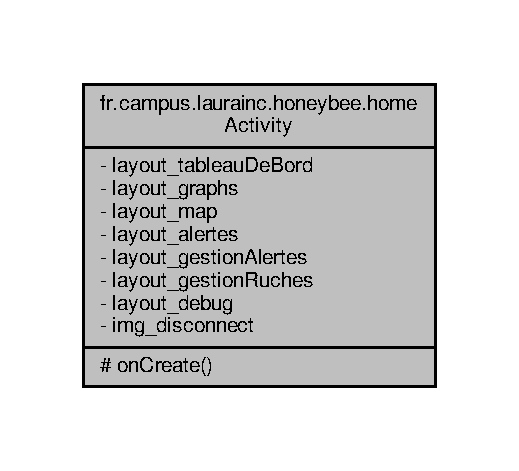
\includegraphics[width=249pt]{classfr_1_1campus_1_1laurainc_1_1honeybee_1_1home_activity__coll__graph}
\end{center}
\end{figure}
\subsubsection*{Fonctions membres protégées}
\begin{DoxyCompactItemize}
\item 
void \hyperlink{classfr_1_1campus_1_1laurainc_1_1honeybee_1_1home_activity_a2fbd2e53b0138742f01d58ee454fb502}{on\+Create} (Bundle saved\+Instance\+State)
\end{DoxyCompactItemize}
\subsubsection*{Attributs privés}
\begin{DoxyCompactItemize}
\item 
Linear\+Layout \hyperlink{classfr_1_1campus_1_1laurainc_1_1honeybee_1_1home_activity_add46240b2690229c03b49cffa3ba76bb}{layout\+\_\+tableau\+De\+Bord}
\item 
Linear\+Layout \hyperlink{classfr_1_1campus_1_1laurainc_1_1honeybee_1_1home_activity_acb650487a892f3446ae3f58ef01733b7}{layout\+\_\+graphs}
\item 
Linear\+Layout \hyperlink{classfr_1_1campus_1_1laurainc_1_1honeybee_1_1home_activity_a12f9873ae11f7d8e187600d58406c4da}{layout\+\_\+map}
\item 
Linear\+Layout \hyperlink{classfr_1_1campus_1_1laurainc_1_1honeybee_1_1home_activity_aee95283002ad6087e895fa0fa51c5030}{layout\+\_\+alertes}
\item 
Linear\+Layout \hyperlink{classfr_1_1campus_1_1laurainc_1_1honeybee_1_1home_activity_a6502d793c6b5c6df0c3b051b2bacab9b}{layout\+\_\+gestion\+Alertes}
\item 
Linear\+Layout \hyperlink{classfr_1_1campus_1_1laurainc_1_1honeybee_1_1home_activity_aea8efb6a37f29b1a122844dcd3e26c0b}{layout\+\_\+gestion\+Ruches}
\item 
Linear\+Layout \hyperlink{classfr_1_1campus_1_1laurainc_1_1honeybee_1_1home_activity_a513adcf5f7471faf27a0e7a2798caf56}{layout\+\_\+debug}
\item 
Image\+View \hyperlink{classfr_1_1campus_1_1laurainc_1_1honeybee_1_1home_activity_ae29a1e0dd983c9e9f5554d37d6fc763e}{img\+\_\+disconnect}
\end{DoxyCompactItemize}


\subsubsection{Documentation des fonctions membres}
\mbox{\Hypertarget{classfr_1_1campus_1_1laurainc_1_1honeybee_1_1home_activity_a2fbd2e53b0138742f01d58ee454fb502}\label{classfr_1_1campus_1_1laurainc_1_1honeybee_1_1home_activity_a2fbd2e53b0138742f01d58ee454fb502}} 
\index{fr\+::campus\+::laurainc\+::honeybee\+::home\+Activity@{fr\+::campus\+::laurainc\+::honeybee\+::home\+Activity}!on\+Create@{on\+Create}}
\index{on\+Create@{on\+Create}!fr\+::campus\+::laurainc\+::honeybee\+::home\+Activity@{fr\+::campus\+::laurainc\+::honeybee\+::home\+Activity}}
\paragraph{\texorpdfstring{on\+Create()}{onCreate()}}
{\footnotesize\ttfamily void fr.\+campus.\+laurainc.\+honeybee.\+home\+Activity.\+on\+Create (\begin{DoxyParamCaption}\item[{Bundle}]{saved\+Instance\+State }\end{DoxyParamCaption})\hspace{0.3cm}{\ttfamily [protected]}}


\begin{DoxyCode}
00022                                                        \{
00023         super.onCreate(savedInstanceState);
00024         setContentView(R.layout.activity\_home);
00025 
00026         \hyperlink{classfr_1_1campus_1_1laurainc_1_1honeybee_1_1home_activity_add46240b2690229c03b49cffa3ba76bb}{layout\_tableauDeBord} = findViewById(R.id.layout\_tableauDeBord);
00027         \hyperlink{classfr_1_1campus_1_1laurainc_1_1honeybee_1_1home_activity_acb650487a892f3446ae3f58ef01733b7}{layout\_graphs} = findViewById(R.id.layout\_graphs);
00028         \hyperlink{classfr_1_1campus_1_1laurainc_1_1honeybee_1_1home_activity_aee95283002ad6087e895fa0fa51c5030}{layout\_alertes} = findViewById(R.id.layout\_alertes);
00029         \hyperlink{classfr_1_1campus_1_1laurainc_1_1honeybee_1_1home_activity_a6502d793c6b5c6df0c3b051b2bacab9b}{layout\_gestionAlertes} = findViewById(R.id.layout\_gestionAlertes);
00030         \hyperlink{classfr_1_1campus_1_1laurainc_1_1honeybee_1_1home_activity_aea8efb6a37f29b1a122844dcd3e26c0b}{layout\_gestionRuches} = findViewById(R.id.layout\_gestionRuche);
00031         \hyperlink{classfr_1_1campus_1_1laurainc_1_1honeybee_1_1home_activity_a513adcf5f7471faf27a0e7a2798caf56}{layout\_debug} = findViewById(R.id.layout\_debug);
00032         \hyperlink{classfr_1_1campus_1_1laurainc_1_1honeybee_1_1home_activity_ae29a1e0dd983c9e9f5554d37d6fc763e}{img\_disconnect} = findViewById(R.id.img\_disconnect);
00033 
00034 
00035         \textcolor{keyword}{final} Intent tableauDeBord = \textcolor{keyword}{new} Intent(homeActivity.this, DashboardActivity.class);
00036         \hyperlink{classfr_1_1campus_1_1laurainc_1_1honeybee_1_1home_activity_add46240b2690229c03b49cffa3ba76bb}{layout\_tableauDeBord}.setOnClickListener(\textcolor{keyword}{new} View.OnClickListener() \{
00037             @Override
00038             \textcolor{keyword}{public} \textcolor{keywordtype}{void} onClick(View v)
00039             \{
00040                 startActivity(tableauDeBord);
00041             \}
00042         \});
00043 
00044         \textcolor{keyword}{final} Intent graphique = \textcolor{keyword}{new} Intent(homeActivity.this, GraphActivity.class);
00045         \hyperlink{classfr_1_1campus_1_1laurainc_1_1honeybee_1_1home_activity_acb650487a892f3446ae3f58ef01733b7}{layout\_graphs}.setOnClickListener(\textcolor{keyword}{new} View.OnClickListener() \{
00046             @Override
00047             \textcolor{keyword}{public} \textcolor{keywordtype}{void} onClick(View v)
00048             \{
00049                 startActivity(graphique);
00050             \}
00051         \});
00052 
00053 
00054         \textcolor{keyword}{final} Intent gestionRuche = \textcolor{keyword}{new} Intent(homeActivity.this, NouvelleRucheActivity.class);
00055         \hyperlink{classfr_1_1campus_1_1laurainc_1_1honeybee_1_1home_activity_aea8efb6a37f29b1a122844dcd3e26c0b}{layout\_gestionRuches}.setOnClickListener(\textcolor{keyword}{new} View.OnClickListener() \{
00056             @Override
00057             \textcolor{keyword}{public} \textcolor{keywordtype}{void} onClick(View v)
00058             \{
00059                 startActivity(gestionRuche);
00060             \}
00061         \});
00062         \textcolor{keyword}{final} Intent disconnect = \textcolor{keyword}{new} Intent(homeActivity.this, MainActivity.class);
00063         \hyperlink{classfr_1_1campus_1_1laurainc_1_1honeybee_1_1home_activity_ae29a1e0dd983c9e9f5554d37d6fc763e}{img\_disconnect}.setOnClickListener(\textcolor{keyword}{new} View.OnClickListener() \{
00064             @Override
00065             \textcolor{keyword}{public} \textcolor{keywordtype}{void} onClick(View v)
00066             \{
00067                 startActivity(disconnect);
00068             \}
00069         \});
00070 
00071         \textcolor{keyword}{final} Intent alertes = \textcolor{keyword}{new} Intent(homeActivity.this, alertesActivity.class);
00072         \hyperlink{classfr_1_1campus_1_1laurainc_1_1honeybee_1_1home_activity_aee95283002ad6087e895fa0fa51c5030}{layout\_alertes}.setOnClickListener(\textcolor{keyword}{new} View.OnClickListener() \{
00073             @Override
00074             \textcolor{keyword}{public} \textcolor{keywordtype}{void} onClick(View v)
00075             \{
00076                 startActivity(alertes);
00077             \}
00078         \});
00079 
00080     \}
\end{DoxyCode}


\subsubsection{Documentation des données membres}
\mbox{\Hypertarget{classfr_1_1campus_1_1laurainc_1_1honeybee_1_1home_activity_ae29a1e0dd983c9e9f5554d37d6fc763e}\label{classfr_1_1campus_1_1laurainc_1_1honeybee_1_1home_activity_ae29a1e0dd983c9e9f5554d37d6fc763e}} 
\index{fr\+::campus\+::laurainc\+::honeybee\+::home\+Activity@{fr\+::campus\+::laurainc\+::honeybee\+::home\+Activity}!img\+\_\+disconnect@{img\+\_\+disconnect}}
\index{img\+\_\+disconnect@{img\+\_\+disconnect}!fr\+::campus\+::laurainc\+::honeybee\+::home\+Activity@{fr\+::campus\+::laurainc\+::honeybee\+::home\+Activity}}
\paragraph{\texorpdfstring{img\+\_\+disconnect}{img\_disconnect}}
{\footnotesize\ttfamily Image\+View fr.\+campus.\+laurainc.\+honeybee.\+home\+Activity.\+img\+\_\+disconnect\hspace{0.3cm}{\ttfamily [private]}}

\mbox{\Hypertarget{classfr_1_1campus_1_1laurainc_1_1honeybee_1_1home_activity_aee95283002ad6087e895fa0fa51c5030}\label{classfr_1_1campus_1_1laurainc_1_1honeybee_1_1home_activity_aee95283002ad6087e895fa0fa51c5030}} 
\index{fr\+::campus\+::laurainc\+::honeybee\+::home\+Activity@{fr\+::campus\+::laurainc\+::honeybee\+::home\+Activity}!layout\+\_\+alertes@{layout\+\_\+alertes}}
\index{layout\+\_\+alertes@{layout\+\_\+alertes}!fr\+::campus\+::laurainc\+::honeybee\+::home\+Activity@{fr\+::campus\+::laurainc\+::honeybee\+::home\+Activity}}
\paragraph{\texorpdfstring{layout\+\_\+alertes}{layout\_alertes}}
{\footnotesize\ttfamily Linear\+Layout fr.\+campus.\+laurainc.\+honeybee.\+home\+Activity.\+layout\+\_\+alertes\hspace{0.3cm}{\ttfamily [private]}}

\mbox{\Hypertarget{classfr_1_1campus_1_1laurainc_1_1honeybee_1_1home_activity_a513adcf5f7471faf27a0e7a2798caf56}\label{classfr_1_1campus_1_1laurainc_1_1honeybee_1_1home_activity_a513adcf5f7471faf27a0e7a2798caf56}} 
\index{fr\+::campus\+::laurainc\+::honeybee\+::home\+Activity@{fr\+::campus\+::laurainc\+::honeybee\+::home\+Activity}!layout\+\_\+debug@{layout\+\_\+debug}}
\index{layout\+\_\+debug@{layout\+\_\+debug}!fr\+::campus\+::laurainc\+::honeybee\+::home\+Activity@{fr\+::campus\+::laurainc\+::honeybee\+::home\+Activity}}
\paragraph{\texorpdfstring{layout\+\_\+debug}{layout\_debug}}
{\footnotesize\ttfamily Linear\+Layout fr.\+campus.\+laurainc.\+honeybee.\+home\+Activity.\+layout\+\_\+debug\hspace{0.3cm}{\ttfamily [private]}}

\mbox{\Hypertarget{classfr_1_1campus_1_1laurainc_1_1honeybee_1_1home_activity_a6502d793c6b5c6df0c3b051b2bacab9b}\label{classfr_1_1campus_1_1laurainc_1_1honeybee_1_1home_activity_a6502d793c6b5c6df0c3b051b2bacab9b}} 
\index{fr\+::campus\+::laurainc\+::honeybee\+::home\+Activity@{fr\+::campus\+::laurainc\+::honeybee\+::home\+Activity}!layout\+\_\+gestion\+Alertes@{layout\+\_\+gestion\+Alertes}}
\index{layout\+\_\+gestion\+Alertes@{layout\+\_\+gestion\+Alertes}!fr\+::campus\+::laurainc\+::honeybee\+::home\+Activity@{fr\+::campus\+::laurainc\+::honeybee\+::home\+Activity}}
\paragraph{\texorpdfstring{layout\+\_\+gestion\+Alertes}{layout\_gestionAlertes}}
{\footnotesize\ttfamily Linear\+Layout fr.\+campus.\+laurainc.\+honeybee.\+home\+Activity.\+layout\+\_\+gestion\+Alertes\hspace{0.3cm}{\ttfamily [private]}}

\mbox{\Hypertarget{classfr_1_1campus_1_1laurainc_1_1honeybee_1_1home_activity_aea8efb6a37f29b1a122844dcd3e26c0b}\label{classfr_1_1campus_1_1laurainc_1_1honeybee_1_1home_activity_aea8efb6a37f29b1a122844dcd3e26c0b}} 
\index{fr\+::campus\+::laurainc\+::honeybee\+::home\+Activity@{fr\+::campus\+::laurainc\+::honeybee\+::home\+Activity}!layout\+\_\+gestion\+Ruches@{layout\+\_\+gestion\+Ruches}}
\index{layout\+\_\+gestion\+Ruches@{layout\+\_\+gestion\+Ruches}!fr\+::campus\+::laurainc\+::honeybee\+::home\+Activity@{fr\+::campus\+::laurainc\+::honeybee\+::home\+Activity}}
\paragraph{\texorpdfstring{layout\+\_\+gestion\+Ruches}{layout\_gestionRuches}}
{\footnotesize\ttfamily Linear\+Layout fr.\+campus.\+laurainc.\+honeybee.\+home\+Activity.\+layout\+\_\+gestion\+Ruches\hspace{0.3cm}{\ttfamily [private]}}

\mbox{\Hypertarget{classfr_1_1campus_1_1laurainc_1_1honeybee_1_1home_activity_acb650487a892f3446ae3f58ef01733b7}\label{classfr_1_1campus_1_1laurainc_1_1honeybee_1_1home_activity_acb650487a892f3446ae3f58ef01733b7}} 
\index{fr\+::campus\+::laurainc\+::honeybee\+::home\+Activity@{fr\+::campus\+::laurainc\+::honeybee\+::home\+Activity}!layout\+\_\+graphs@{layout\+\_\+graphs}}
\index{layout\+\_\+graphs@{layout\+\_\+graphs}!fr\+::campus\+::laurainc\+::honeybee\+::home\+Activity@{fr\+::campus\+::laurainc\+::honeybee\+::home\+Activity}}
\paragraph{\texorpdfstring{layout\+\_\+graphs}{layout\_graphs}}
{\footnotesize\ttfamily Linear\+Layout fr.\+campus.\+laurainc.\+honeybee.\+home\+Activity.\+layout\+\_\+graphs\hspace{0.3cm}{\ttfamily [private]}}

\mbox{\Hypertarget{classfr_1_1campus_1_1laurainc_1_1honeybee_1_1home_activity_a12f9873ae11f7d8e187600d58406c4da}\label{classfr_1_1campus_1_1laurainc_1_1honeybee_1_1home_activity_a12f9873ae11f7d8e187600d58406c4da}} 
\index{fr\+::campus\+::laurainc\+::honeybee\+::home\+Activity@{fr\+::campus\+::laurainc\+::honeybee\+::home\+Activity}!layout\+\_\+map@{layout\+\_\+map}}
\index{layout\+\_\+map@{layout\+\_\+map}!fr\+::campus\+::laurainc\+::honeybee\+::home\+Activity@{fr\+::campus\+::laurainc\+::honeybee\+::home\+Activity}}
\paragraph{\texorpdfstring{layout\+\_\+map}{layout\_map}}
{\footnotesize\ttfamily Linear\+Layout fr.\+campus.\+laurainc.\+honeybee.\+home\+Activity.\+layout\+\_\+map\hspace{0.3cm}{\ttfamily [private]}}

\mbox{\Hypertarget{classfr_1_1campus_1_1laurainc_1_1honeybee_1_1home_activity_add46240b2690229c03b49cffa3ba76bb}\label{classfr_1_1campus_1_1laurainc_1_1honeybee_1_1home_activity_add46240b2690229c03b49cffa3ba76bb}} 
\index{fr\+::campus\+::laurainc\+::honeybee\+::home\+Activity@{fr\+::campus\+::laurainc\+::honeybee\+::home\+Activity}!layout\+\_\+tableau\+De\+Bord@{layout\+\_\+tableau\+De\+Bord}}
\index{layout\+\_\+tableau\+De\+Bord@{layout\+\_\+tableau\+De\+Bord}!fr\+::campus\+::laurainc\+::honeybee\+::home\+Activity@{fr\+::campus\+::laurainc\+::honeybee\+::home\+Activity}}
\paragraph{\texorpdfstring{layout\+\_\+tableau\+De\+Bord}{layout\_tableauDeBord}}
{\footnotesize\ttfamily Linear\+Layout fr.\+campus.\+laurainc.\+honeybee.\+home\+Activity.\+layout\+\_\+tableau\+De\+Bord\hspace{0.3cm}{\ttfamily [private]}}



La documentation de cette classe a été générée à partir du fichier suivant \+:\begin{DoxyCompactItemize}
\item 
\hyperlink{home_activity_8java}{home\+Activity.\+java}\end{DoxyCompactItemize}

\hypertarget{classfr_1_1campus_1_1laurainc_1_1honeybee_1_1_honey_bee}{}\subsection{Référence de la classe fr.\+campus.\+laurainc.\+honeybee.\+Honey\+Bee}
\label{classfr_1_1campus_1_1laurainc_1_1honeybee_1_1_honey_bee}\index{fr.\+campus.\+laurainc.\+honeybee.\+Honey\+Bee@{fr.\+campus.\+laurainc.\+honeybee.\+Honey\+Bee}}


Paramètres globaux de l\textquotesingle{}application.  




Graphe de collaboration de fr.\+campus.\+laurainc.\+honeybee.\+Honey\+Bee\+:\nopagebreak
\begin{figure}[H]
\begin{center}
\leavevmode
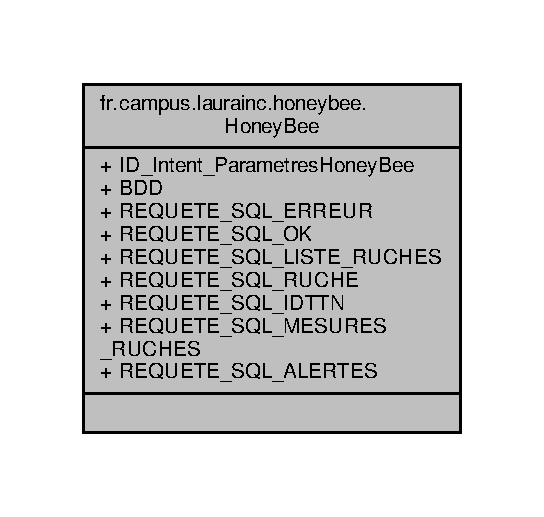
\includegraphics[width=261pt]{classfr_1_1campus_1_1laurainc_1_1honeybee_1_1_honey_bee__coll__graph}
\end{center}
\end{figure}
\subsubsection*{Attributs publics statiques}
\begin{DoxyCompactItemize}
\item 
static final int \hyperlink{classfr_1_1campus_1_1laurainc_1_1honeybee_1_1_honey_bee_a479c42ac63c5c79e26c4836f965171d2}{I\+D\+\_\+\+Intent\+\_\+\+Parametres\+Honey\+Bee} = 1
\begin{DoxyCompactList}\small\item\em l\textquotesingle{}ID de l\textquotesingle{}Intent \hyperlink{classfr_1_1campus_1_1laurainc_1_1honeybee_1_1_parametres_honey_bee_activity}{Parametres\+Honey\+Bee\+Activity} \end{DoxyCompactList}\item 
static final boolean \hyperlink{classfr_1_1campus_1_1laurainc_1_1honeybee_1_1_honey_bee_abfb4f6cc1c8bb793c37ccb8408abc51c}{B\+DD} = true
\begin{DoxyCompactList}\small\item\em si vrai l\textquotesingle{}application peut utiliser la base de données My\+S\+QL (utile en debug) \end{DoxyCompactList}\item 
static final int \hyperlink{classfr_1_1campus_1_1laurainc_1_1honeybee_1_1_honey_bee_a275b7a8582c8193ff444d21928ef7e36}{R\+E\+Q\+U\+E\+T\+E\+\_\+\+S\+Q\+L\+\_\+\+E\+R\+R\+E\+UR} = -\/1
\item 
static final int \hyperlink{classfr_1_1campus_1_1laurainc_1_1honeybee_1_1_honey_bee_a793e7851c6d203b52a1486d1e6c9bbc7}{R\+E\+Q\+U\+E\+T\+E\+\_\+\+S\+Q\+L\+\_\+\+OK} = 0
\item 
static final int \hyperlink{classfr_1_1campus_1_1laurainc_1_1honeybee_1_1_honey_bee_afd5c8c4447e00d9a75eb95f83a62a860}{R\+E\+Q\+U\+E\+T\+E\+\_\+\+S\+Q\+L\+\_\+\+L\+I\+S\+T\+E\+\_\+\+R\+U\+C\+H\+ES} = 1
\item 
static final int \hyperlink{classfr_1_1campus_1_1laurainc_1_1honeybee_1_1_honey_bee_a933d238d27d6b17df6f65bef23a2de1d}{R\+E\+Q\+U\+E\+T\+E\+\_\+\+S\+Q\+L\+\_\+\+R\+U\+C\+HE} = 2
\item 
static final int \hyperlink{classfr_1_1campus_1_1laurainc_1_1honeybee_1_1_honey_bee_a114d1a573571b6a77a2d0e48a0ee3d5c}{R\+E\+Q\+U\+E\+T\+E\+\_\+\+S\+Q\+L\+\_\+\+I\+D\+T\+TN} =3
\item 
static final int \hyperlink{classfr_1_1campus_1_1laurainc_1_1honeybee_1_1_honey_bee_aa6c2993ef079afd106565e2748b72156}{R\+E\+Q\+U\+E\+T\+E\+\_\+\+S\+Q\+L\+\_\+\+M\+E\+S\+U\+R\+E\+S\+\_\+\+R\+U\+C\+H\+ES} = 4
\item 
static final int \hyperlink{classfr_1_1campus_1_1laurainc_1_1honeybee_1_1_honey_bee_a30fce22196d286c02fbcdd7629401c8a}{R\+E\+Q\+U\+E\+T\+E\+\_\+\+S\+Q\+L\+\_\+\+A\+L\+E\+R\+T\+ES} = 5
\end{DoxyCompactItemize}


\subsubsection{Description détaillée}
\begin{DoxyAuthor}{Auteur}
Thierry Vaira 
\end{DoxyAuthor}


\subsubsection{Documentation des données membres}
\mbox{\Hypertarget{classfr_1_1campus_1_1laurainc_1_1honeybee_1_1_honey_bee_abfb4f6cc1c8bb793c37ccb8408abc51c}\label{classfr_1_1campus_1_1laurainc_1_1honeybee_1_1_honey_bee_abfb4f6cc1c8bb793c37ccb8408abc51c}} 
\index{fr\+::campus\+::laurainc\+::honeybee\+::\+Honey\+Bee@{fr\+::campus\+::laurainc\+::honeybee\+::\+Honey\+Bee}!B\+DD@{B\+DD}}
\index{B\+DD@{B\+DD}!fr\+::campus\+::laurainc\+::honeybee\+::\+Honey\+Bee@{fr\+::campus\+::laurainc\+::honeybee\+::\+Honey\+Bee}}
\paragraph{\texorpdfstring{B\+DD}{BDD}}
{\footnotesize\ttfamily final boolean fr.\+campus.\+laurainc.\+honeybee.\+Honey\+Bee.\+B\+DD = true\hspace{0.3cm}{\ttfamily [static]}}



Référencé par \hyperlink{classfr_1_1campus_1_1laurainc_1_1honeybee_1_1_base_de_donnees_a08564ea7dccde161d6eac4b8879401bb}{fr.\+campus.\+laurainc.\+honeybee.\+Base\+De\+Donnees.\+connecter()}, \hyperlink{classfr_1_1campus_1_1laurainc_1_1honeybee_1_1_base_de_donnees_ae022ff0b4923d637f8d392cb908aa252}{fr.\+campus.\+laurainc.\+honeybee.\+Base\+De\+Donnees.\+deconnecter()}, \hyperlink{classfr_1_1campus_1_1laurainc_1_1honeybee_1_1_base_de_donnees_a735f54c2c183a595c9a9a5ba947491f5}{fr.\+campus.\+laurainc.\+honeybee.\+Base\+De\+Donnees.\+est\+Connecte()}, \hyperlink{classfr_1_1campus_1_1laurainc_1_1honeybee_1_1_base_de_donnees_a421bffe6f14c01bee64695e7b6a9745d}{fr.\+campus.\+laurainc.\+honeybee.\+Base\+De\+Donnees.\+executer\+Requete()}, \hyperlink{classfr_1_1campus_1_1laurainc_1_1honeybee_1_1_nouvelle_ruche_activity_ae97fec78fb0a2e1cc4610182bc71ea0d}{fr.\+campus.\+laurainc.\+honeybee.\+Nouvelle\+Ruche\+Activity.\+on\+Create()}, \hyperlink{classfr_1_1campus_1_1laurainc_1_1honeybee_1_1_base_de_donnees_a89357a1cc8a3648400df37a8bfe95958}{fr.\+campus.\+laurainc.\+honeybee.\+Base\+De\+Donnees.\+reconnecter()}, \hyperlink{classfr_1_1campus_1_1laurainc_1_1honeybee_1_1_ruche_a7a99d3c585f2c507eb2c6c265a5bb1fe}{fr.\+campus.\+laurainc.\+honeybee.\+Ruche.\+recuperer()}, \hyperlink{classfr_1_1campus_1_1laurainc_1_1honeybee_1_1_ruche_ade5d681bd0a29d84e0d069169b10a38b}{fr.\+campus.\+laurainc.\+honeybee.\+Ruche.\+recuperer\+Choix\+Ch\+App\+I\+D()}, \hyperlink{classfr_1_1campus_1_1laurainc_1_1honeybee_1_1_ruche_ace10a52a470257f2b8f161fc3c7b9f15}{fr.\+campus.\+laurainc.\+honeybee.\+Ruche.\+recuperer\+Historique\+Alertes()}, \hyperlink{classfr_1_1campus_1_1laurainc_1_1honeybee_1_1_ruche_a1113f3b4a527a801fdf50350667fd212}{fr.\+campus.\+laurainc.\+honeybee.\+Ruche.\+recuperer\+Id\+T\+T\+N()}, \hyperlink{classfr_1_1campus_1_1laurainc_1_1honeybee_1_1_ruche_aba0591cda391b907da41a0afeba4d59d}{fr.\+campus.\+laurainc.\+honeybee.\+Ruche.\+recuperer\+Liste\+Ruches()}, \hyperlink{classfr_1_1campus_1_1laurainc_1_1honeybee_1_1_ruche_a84de3c3af21b1cbeae2075e480acaabc}{fr.\+campus.\+laurainc.\+honeybee.\+Ruche.\+recuperer\+Mesures\+Journalieres\+Ruche()}, \hyperlink{classfr_1_1campus_1_1laurainc_1_1honeybee_1_1_ruche_a94f815b44f0d5d8682833d6b6e783713}{fr.\+campus.\+laurainc.\+honeybee.\+Ruche.\+recuperer\+Moyennes()}, \hyperlink{classfr_1_1campus_1_1laurainc_1_1honeybee_1_1_ruche_a56ec53516e4f94b4f5e42f083fa345db}{fr.\+campus.\+laurainc.\+honeybee.\+Ruche.\+Ruche()}, et \hyperlink{classfr_1_1campus_1_1laurainc_1_1honeybee_1_1_base_de_donnees_a7b0977566d74684fab184f7a5efce3c8}{fr.\+campus.\+laurainc.\+honeybee.\+Base\+De\+Donnees.\+supprimer\+Ruche()}.

\mbox{\Hypertarget{classfr_1_1campus_1_1laurainc_1_1honeybee_1_1_honey_bee_a479c42ac63c5c79e26c4836f965171d2}\label{classfr_1_1campus_1_1laurainc_1_1honeybee_1_1_honey_bee_a479c42ac63c5c79e26c4836f965171d2}} 
\index{fr\+::campus\+::laurainc\+::honeybee\+::\+Honey\+Bee@{fr\+::campus\+::laurainc\+::honeybee\+::\+Honey\+Bee}!I\+D\+\_\+\+Intent\+\_\+\+Parametres\+Honey\+Bee@{I\+D\+\_\+\+Intent\+\_\+\+Parametres\+Honey\+Bee}}
\index{I\+D\+\_\+\+Intent\+\_\+\+Parametres\+Honey\+Bee@{I\+D\+\_\+\+Intent\+\_\+\+Parametres\+Honey\+Bee}!fr\+::campus\+::laurainc\+::honeybee\+::\+Honey\+Bee@{fr\+::campus\+::laurainc\+::honeybee\+::\+Honey\+Bee}}
\paragraph{\texorpdfstring{I\+D\+\_\+\+Intent\+\_\+\+Parametres\+Honey\+Bee}{ID\_Intent\_ParametresHoneyBee}}
{\footnotesize\ttfamily final int fr.\+campus.\+laurainc.\+honeybee.\+Honey\+Bee.\+I\+D\+\_\+\+Intent\+\_\+\+Parametres\+Honey\+Bee = 1\hspace{0.3cm}{\ttfamily [static]}}



Référencé par \hyperlink{classfr_1_1campus_1_1laurainc_1_1honeybee_1_1_main_activity_ae751b46f1881bda6b3b0e08025a9c044}{fr.\+campus.\+laurainc.\+honeybee.\+Main\+Activity.\+on\+Activity\+Result()}.

\mbox{\Hypertarget{classfr_1_1campus_1_1laurainc_1_1honeybee_1_1_honey_bee_a30fce22196d286c02fbcdd7629401c8a}\label{classfr_1_1campus_1_1laurainc_1_1honeybee_1_1_honey_bee_a30fce22196d286c02fbcdd7629401c8a}} 
\index{fr\+::campus\+::laurainc\+::honeybee\+::\+Honey\+Bee@{fr\+::campus\+::laurainc\+::honeybee\+::\+Honey\+Bee}!R\+E\+Q\+U\+E\+T\+E\+\_\+\+S\+Q\+L\+\_\+\+A\+L\+E\+R\+T\+ES@{R\+E\+Q\+U\+E\+T\+E\+\_\+\+S\+Q\+L\+\_\+\+A\+L\+E\+R\+T\+ES}}
\index{R\+E\+Q\+U\+E\+T\+E\+\_\+\+S\+Q\+L\+\_\+\+A\+L\+E\+R\+T\+ES@{R\+E\+Q\+U\+E\+T\+E\+\_\+\+S\+Q\+L\+\_\+\+A\+L\+E\+R\+T\+ES}!fr\+::campus\+::laurainc\+::honeybee\+::\+Honey\+Bee@{fr\+::campus\+::laurainc\+::honeybee\+::\+Honey\+Bee}}
\paragraph{\texorpdfstring{R\+E\+Q\+U\+E\+T\+E\+\_\+\+S\+Q\+L\+\_\+\+A\+L\+E\+R\+T\+ES}{REQUETE\_SQL\_ALERTES}}
{\footnotesize\ttfamily final int fr.\+campus.\+laurainc.\+honeybee.\+Honey\+Bee.\+R\+E\+Q\+U\+E\+T\+E\+\_\+\+S\+Q\+L\+\_\+\+A\+L\+E\+R\+T\+ES = 5\hspace{0.3cm}{\ttfamily [static]}}



Référencé par \hyperlink{classfr_1_1campus_1_1laurainc_1_1honeybee_1_1_ruche_ace10a52a470257f2b8f161fc3c7b9f15}{fr.\+campus.\+laurainc.\+honeybee.\+Ruche.\+recuperer\+Historique\+Alertes()}.

\mbox{\Hypertarget{classfr_1_1campus_1_1laurainc_1_1honeybee_1_1_honey_bee_a275b7a8582c8193ff444d21928ef7e36}\label{classfr_1_1campus_1_1laurainc_1_1honeybee_1_1_honey_bee_a275b7a8582c8193ff444d21928ef7e36}} 
\index{fr\+::campus\+::laurainc\+::honeybee\+::\+Honey\+Bee@{fr\+::campus\+::laurainc\+::honeybee\+::\+Honey\+Bee}!R\+E\+Q\+U\+E\+T\+E\+\_\+\+S\+Q\+L\+\_\+\+E\+R\+R\+E\+UR@{R\+E\+Q\+U\+E\+T\+E\+\_\+\+S\+Q\+L\+\_\+\+E\+R\+R\+E\+UR}}
\index{R\+E\+Q\+U\+E\+T\+E\+\_\+\+S\+Q\+L\+\_\+\+E\+R\+R\+E\+UR@{R\+E\+Q\+U\+E\+T\+E\+\_\+\+S\+Q\+L\+\_\+\+E\+R\+R\+E\+UR}!fr\+::campus\+::laurainc\+::honeybee\+::\+Honey\+Bee@{fr\+::campus\+::laurainc\+::honeybee\+::\+Honey\+Bee}}
\paragraph{\texorpdfstring{R\+E\+Q\+U\+E\+T\+E\+\_\+\+S\+Q\+L\+\_\+\+E\+R\+R\+E\+UR}{REQUETE\_SQL\_ERREUR}}
{\footnotesize\ttfamily final int fr.\+campus.\+laurainc.\+honeybee.\+Honey\+Bee.\+R\+E\+Q\+U\+E\+T\+E\+\_\+\+S\+Q\+L\+\_\+\+E\+R\+R\+E\+UR = -\/1\hspace{0.3cm}{\ttfamily [static]}}



Référencé par \hyperlink{classfr_1_1campus_1_1laurainc_1_1honeybee_1_1_ruche_a7a99d3c585f2c507eb2c6c265a5bb1fe}{fr.\+campus.\+laurainc.\+honeybee.\+Ruche.\+recuperer()}, \hyperlink{classfr_1_1campus_1_1laurainc_1_1honeybee_1_1_ruche_ade5d681bd0a29d84e0d069169b10a38b}{fr.\+campus.\+laurainc.\+honeybee.\+Ruche.\+recuperer\+Choix\+Ch\+App\+I\+D()}, \hyperlink{classfr_1_1campus_1_1laurainc_1_1honeybee_1_1_ruche_ace10a52a470257f2b8f161fc3c7b9f15}{fr.\+campus.\+laurainc.\+honeybee.\+Ruche.\+recuperer\+Historique\+Alertes()}, \hyperlink{classfr_1_1campus_1_1laurainc_1_1honeybee_1_1_ruche_a1113f3b4a527a801fdf50350667fd212}{fr.\+campus.\+laurainc.\+honeybee.\+Ruche.\+recuperer\+Id\+T\+T\+N()}, \hyperlink{classfr_1_1campus_1_1laurainc_1_1honeybee_1_1_ruche_aba0591cda391b907da41a0afeba4d59d}{fr.\+campus.\+laurainc.\+honeybee.\+Ruche.\+recuperer\+Liste\+Ruches()}, \hyperlink{classfr_1_1campus_1_1laurainc_1_1honeybee_1_1_ruche_a84de3c3af21b1cbeae2075e480acaabc}{fr.\+campus.\+laurainc.\+honeybee.\+Ruche.\+recuperer\+Mesures\+Journalieres\+Ruche()}, et \hyperlink{classfr_1_1campus_1_1laurainc_1_1honeybee_1_1_ruche_a94f815b44f0d5d8682833d6b6e783713}{fr.\+campus.\+laurainc.\+honeybee.\+Ruche.\+recuperer\+Moyennes()}.

\mbox{\Hypertarget{classfr_1_1campus_1_1laurainc_1_1honeybee_1_1_honey_bee_a114d1a573571b6a77a2d0e48a0ee3d5c}\label{classfr_1_1campus_1_1laurainc_1_1honeybee_1_1_honey_bee_a114d1a573571b6a77a2d0e48a0ee3d5c}} 
\index{fr\+::campus\+::laurainc\+::honeybee\+::\+Honey\+Bee@{fr\+::campus\+::laurainc\+::honeybee\+::\+Honey\+Bee}!R\+E\+Q\+U\+E\+T\+E\+\_\+\+S\+Q\+L\+\_\+\+I\+D\+T\+TN@{R\+E\+Q\+U\+E\+T\+E\+\_\+\+S\+Q\+L\+\_\+\+I\+D\+T\+TN}}
\index{R\+E\+Q\+U\+E\+T\+E\+\_\+\+S\+Q\+L\+\_\+\+I\+D\+T\+TN@{R\+E\+Q\+U\+E\+T\+E\+\_\+\+S\+Q\+L\+\_\+\+I\+D\+T\+TN}!fr\+::campus\+::laurainc\+::honeybee\+::\+Honey\+Bee@{fr\+::campus\+::laurainc\+::honeybee\+::\+Honey\+Bee}}
\paragraph{\texorpdfstring{R\+E\+Q\+U\+E\+T\+E\+\_\+\+S\+Q\+L\+\_\+\+I\+D\+T\+TN}{REQUETE\_SQL\_IDTTN}}
{\footnotesize\ttfamily final int fr.\+campus.\+laurainc.\+honeybee.\+Honey\+Bee.\+R\+E\+Q\+U\+E\+T\+E\+\_\+\+S\+Q\+L\+\_\+\+I\+D\+T\+TN =3\hspace{0.3cm}{\ttfamily [static]}}



Référencé par \hyperlink{classfr_1_1campus_1_1laurainc_1_1honeybee_1_1_ruche_a1113f3b4a527a801fdf50350667fd212}{fr.\+campus.\+laurainc.\+honeybee.\+Ruche.\+recuperer\+Id\+T\+T\+N()}, et \hyperlink{classfr_1_1campus_1_1laurainc_1_1honeybee_1_1_ruche_a94f815b44f0d5d8682833d6b6e783713}{fr.\+campus.\+laurainc.\+honeybee.\+Ruche.\+recuperer\+Moyennes()}.

\mbox{\Hypertarget{classfr_1_1campus_1_1laurainc_1_1honeybee_1_1_honey_bee_afd5c8c4447e00d9a75eb95f83a62a860}\label{classfr_1_1campus_1_1laurainc_1_1honeybee_1_1_honey_bee_afd5c8c4447e00d9a75eb95f83a62a860}} 
\index{fr\+::campus\+::laurainc\+::honeybee\+::\+Honey\+Bee@{fr\+::campus\+::laurainc\+::honeybee\+::\+Honey\+Bee}!R\+E\+Q\+U\+E\+T\+E\+\_\+\+S\+Q\+L\+\_\+\+L\+I\+S\+T\+E\+\_\+\+R\+U\+C\+H\+ES@{R\+E\+Q\+U\+E\+T\+E\+\_\+\+S\+Q\+L\+\_\+\+L\+I\+S\+T\+E\+\_\+\+R\+U\+C\+H\+ES}}
\index{R\+E\+Q\+U\+E\+T\+E\+\_\+\+S\+Q\+L\+\_\+\+L\+I\+S\+T\+E\+\_\+\+R\+U\+C\+H\+ES@{R\+E\+Q\+U\+E\+T\+E\+\_\+\+S\+Q\+L\+\_\+\+L\+I\+S\+T\+E\+\_\+\+R\+U\+C\+H\+ES}!fr\+::campus\+::laurainc\+::honeybee\+::\+Honey\+Bee@{fr\+::campus\+::laurainc\+::honeybee\+::\+Honey\+Bee}}
\paragraph{\texorpdfstring{R\+E\+Q\+U\+E\+T\+E\+\_\+\+S\+Q\+L\+\_\+\+L\+I\+S\+T\+E\+\_\+\+R\+U\+C\+H\+ES}{REQUETE\_SQL\_LISTE\_RUCHES}}
{\footnotesize\ttfamily final int fr.\+campus.\+laurainc.\+honeybee.\+Honey\+Bee.\+R\+E\+Q\+U\+E\+T\+E\+\_\+\+S\+Q\+L\+\_\+\+L\+I\+S\+T\+E\+\_\+\+R\+U\+C\+H\+ES = 1\hspace{0.3cm}{\ttfamily [static]}}



Référencé par \hyperlink{classfr_1_1campus_1_1laurainc_1_1honeybee_1_1_ruche_ade5d681bd0a29d84e0d069169b10a38b}{fr.\+campus.\+laurainc.\+honeybee.\+Ruche.\+recuperer\+Choix\+Ch\+App\+I\+D()}, et \hyperlink{classfr_1_1campus_1_1laurainc_1_1honeybee_1_1_ruche_aba0591cda391b907da41a0afeba4d59d}{fr.\+campus.\+laurainc.\+honeybee.\+Ruche.\+recuperer\+Liste\+Ruches()}.

\mbox{\Hypertarget{classfr_1_1campus_1_1laurainc_1_1honeybee_1_1_honey_bee_aa6c2993ef079afd106565e2748b72156}\label{classfr_1_1campus_1_1laurainc_1_1honeybee_1_1_honey_bee_aa6c2993ef079afd106565e2748b72156}} 
\index{fr\+::campus\+::laurainc\+::honeybee\+::\+Honey\+Bee@{fr\+::campus\+::laurainc\+::honeybee\+::\+Honey\+Bee}!R\+E\+Q\+U\+E\+T\+E\+\_\+\+S\+Q\+L\+\_\+\+M\+E\+S\+U\+R\+E\+S\+\_\+\+R\+U\+C\+H\+ES@{R\+E\+Q\+U\+E\+T\+E\+\_\+\+S\+Q\+L\+\_\+\+M\+E\+S\+U\+R\+E\+S\+\_\+\+R\+U\+C\+H\+ES}}
\index{R\+E\+Q\+U\+E\+T\+E\+\_\+\+S\+Q\+L\+\_\+\+M\+E\+S\+U\+R\+E\+S\+\_\+\+R\+U\+C\+H\+ES@{R\+E\+Q\+U\+E\+T\+E\+\_\+\+S\+Q\+L\+\_\+\+M\+E\+S\+U\+R\+E\+S\+\_\+\+R\+U\+C\+H\+ES}!fr\+::campus\+::laurainc\+::honeybee\+::\+Honey\+Bee@{fr\+::campus\+::laurainc\+::honeybee\+::\+Honey\+Bee}}
\paragraph{\texorpdfstring{R\+E\+Q\+U\+E\+T\+E\+\_\+\+S\+Q\+L\+\_\+\+M\+E\+S\+U\+R\+E\+S\+\_\+\+R\+U\+C\+H\+ES}{REQUETE\_SQL\_MESURES\_RUCHES}}
{\footnotesize\ttfamily final int fr.\+campus.\+laurainc.\+honeybee.\+Honey\+Bee.\+R\+E\+Q\+U\+E\+T\+E\+\_\+\+S\+Q\+L\+\_\+\+M\+E\+S\+U\+R\+E\+S\+\_\+\+R\+U\+C\+H\+ES = 4\hspace{0.3cm}{\ttfamily [static]}}



Référencé par \hyperlink{classfr_1_1campus_1_1laurainc_1_1honeybee_1_1_ruche_a84de3c3af21b1cbeae2075e480acaabc}{fr.\+campus.\+laurainc.\+honeybee.\+Ruche.\+recuperer\+Mesures\+Journalieres\+Ruche()}.

\mbox{\Hypertarget{classfr_1_1campus_1_1laurainc_1_1honeybee_1_1_honey_bee_a793e7851c6d203b52a1486d1e6c9bbc7}\label{classfr_1_1campus_1_1laurainc_1_1honeybee_1_1_honey_bee_a793e7851c6d203b52a1486d1e6c9bbc7}} 
\index{fr\+::campus\+::laurainc\+::honeybee\+::\+Honey\+Bee@{fr\+::campus\+::laurainc\+::honeybee\+::\+Honey\+Bee}!R\+E\+Q\+U\+E\+T\+E\+\_\+\+S\+Q\+L\+\_\+\+OK@{R\+E\+Q\+U\+E\+T\+E\+\_\+\+S\+Q\+L\+\_\+\+OK}}
\index{R\+E\+Q\+U\+E\+T\+E\+\_\+\+S\+Q\+L\+\_\+\+OK@{R\+E\+Q\+U\+E\+T\+E\+\_\+\+S\+Q\+L\+\_\+\+OK}!fr\+::campus\+::laurainc\+::honeybee\+::\+Honey\+Bee@{fr\+::campus\+::laurainc\+::honeybee\+::\+Honey\+Bee}}
\paragraph{\texorpdfstring{R\+E\+Q\+U\+E\+T\+E\+\_\+\+S\+Q\+L\+\_\+\+OK}{REQUETE\_SQL\_OK}}
{\footnotesize\ttfamily final int fr.\+campus.\+laurainc.\+honeybee.\+Honey\+Bee.\+R\+E\+Q\+U\+E\+T\+E\+\_\+\+S\+Q\+L\+\_\+\+OK = 0\hspace{0.3cm}{\ttfamily [static]}}

\mbox{\Hypertarget{classfr_1_1campus_1_1laurainc_1_1honeybee_1_1_honey_bee_a933d238d27d6b17df6f65bef23a2de1d}\label{classfr_1_1campus_1_1laurainc_1_1honeybee_1_1_honey_bee_a933d238d27d6b17df6f65bef23a2de1d}} 
\index{fr\+::campus\+::laurainc\+::honeybee\+::\+Honey\+Bee@{fr\+::campus\+::laurainc\+::honeybee\+::\+Honey\+Bee}!R\+E\+Q\+U\+E\+T\+E\+\_\+\+S\+Q\+L\+\_\+\+R\+U\+C\+HE@{R\+E\+Q\+U\+E\+T\+E\+\_\+\+S\+Q\+L\+\_\+\+R\+U\+C\+HE}}
\index{R\+E\+Q\+U\+E\+T\+E\+\_\+\+S\+Q\+L\+\_\+\+R\+U\+C\+HE@{R\+E\+Q\+U\+E\+T\+E\+\_\+\+S\+Q\+L\+\_\+\+R\+U\+C\+HE}!fr\+::campus\+::laurainc\+::honeybee\+::\+Honey\+Bee@{fr\+::campus\+::laurainc\+::honeybee\+::\+Honey\+Bee}}
\paragraph{\texorpdfstring{R\+E\+Q\+U\+E\+T\+E\+\_\+\+S\+Q\+L\+\_\+\+R\+U\+C\+HE}{REQUETE\_SQL\_RUCHE}}
{\footnotesize\ttfamily final int fr.\+campus.\+laurainc.\+honeybee.\+Honey\+Bee.\+R\+E\+Q\+U\+E\+T\+E\+\_\+\+S\+Q\+L\+\_\+\+R\+U\+C\+HE = 2\hspace{0.3cm}{\ttfamily [static]}}



Référencé par \hyperlink{classfr_1_1campus_1_1laurainc_1_1honeybee_1_1_ruche_a7a99d3c585f2c507eb2c6c265a5bb1fe}{fr.\+campus.\+laurainc.\+honeybee.\+Ruche.\+recuperer()}.



La documentation de cette classe a été générée à partir du fichier suivant \+:\begin{DoxyCompactItemize}
\item 
\hyperlink{_honey_bee_8java}{Honey\+Bee.\+java}\end{DoxyCompactItemize}

\hypertarget{class_infos_batterie}{}\subsection{Référence de la classe Infos\+Batterie}
\label{class_infos_batterie}\index{Infos\+Batterie@{Infos\+Batterie}}


Déclaration de la classe \hyperlink{class_infos_batterie}{Infos\+Batterie}.  




{\ttfamily \#include $<$infos\+Batterie.\+h$>$}



Graphe de collaboration de Infos\+Batterie\+:\nopagebreak
\begin{figure}[H]
\begin{center}
\leavevmode
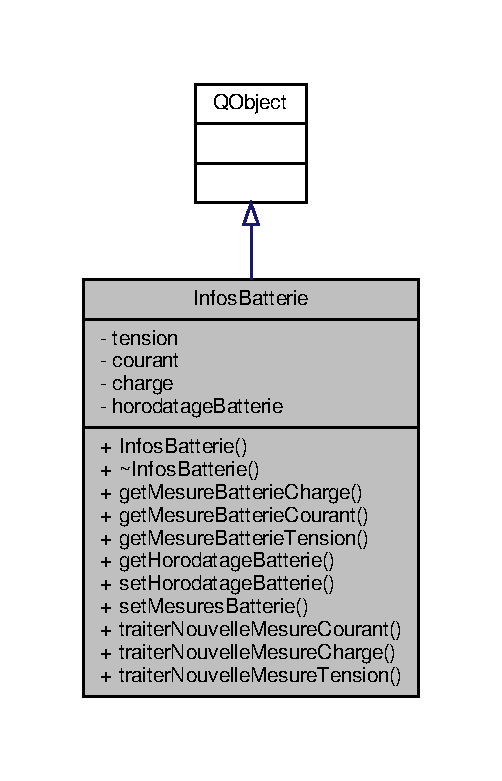
\includegraphics[width=241pt]{class_infos_batterie__coll__graph}
\end{center}
\end{figure}
\subsubsection*{Connecteurs publics}
\begin{DoxyCompactItemize}
\item 
void \hyperlink{class_infos_batterie_a7c127f1798ba279918b7b0783f9d23c4}{traiter\+Nouvelle\+Mesure\+Courant} (Q\+String nouveau\+Courant, Q\+String horodatage)
\item 
void \hyperlink{class_infos_batterie_a92c1afb1e022fe75cd7a0877d64e8d53}{traiter\+Nouvelle\+Mesure\+Charge} (Q\+String nouvelle\+Charge, Q\+String horodatage)
\item 
void \hyperlink{class_infos_batterie_a8b1c1008d441b30f2cf38995fae3e0ca}{traiter\+Nouvelle\+Mesure\+Tension} (Q\+String nouvelle\+Tension, Q\+String horodatage)
\end{DoxyCompactItemize}
\subsubsection*{Signaux}
\begin{DoxyCompactItemize}
\item 
void \hyperlink{class_infos_batterie_a932a48aafb94e5289d775bb3305fdb74}{tension\+Envoye} (const double \hyperlink{class_infos_batterie_a45d09805075337f7f2d4b84d02a2ee47}{tension}, Q\+String)
\item 
void \hyperlink{class_infos_batterie_a3b648bf48c796c64d90db29741889eb1}{courant\+Envoye} (const double \hyperlink{class_infos_batterie_a417f025b2ccddea7d28f80df4413945a}{courant}, Q\+String)
\item 
void \hyperlink{class_infos_batterie_a75ef2e971d86ae3b66a787d53e3d5c63}{charge\+Envoye} (const double \hyperlink{class_infos_batterie_af3ad72cdbbf13f2dec6d81f078a2c0d2}{charge}, Q\+String)
\end{DoxyCompactItemize}
\subsubsection*{Fonctions membres publiques}
\begin{DoxyCompactItemize}
\item 
\hyperlink{class_infos_batterie_a8dea33c2515f2c30ea3a525e17c03fa2}{Infos\+Batterie} (\hyperlink{class_q_object}{Q\+Object} $\ast$parent)
\item 
\hyperlink{class_infos_batterie_a5c59c1d607d25b46fb7c3768a01f4ec5}{$\sim$\+Infos\+Batterie} ()
\item 
double \hyperlink{class_infos_batterie_a8c37174d0d36e4f5ada9d16dd5894803}{get\+Mesure\+Batterie\+Charge} ()
\item 
double \hyperlink{class_infos_batterie_a17a55f19c132026091217c243bf402c0}{get\+Mesure\+Batterie\+Courant} ()
\item 
double \hyperlink{class_infos_batterie_a470b96c2fe1fab6a187c6d0997bd76a8}{get\+Mesure\+Batterie\+Tension} ()
\item 
Q\+String \hyperlink{class_infos_batterie_aeac9a7bcd953444f4f2302d7949c74ef}{get\+Horodatage\+Batterie} ()
\item 
void \hyperlink{class_infos_batterie_a1d98a79696389d0264959d0c8a64bbcd}{set\+Horodatage\+Batterie} (Q\+String \hyperlink{class_infos_batterie_a261067aff87023bccd60e59961ef1ffc}{horodatage\+Batterie})
\item 
void \hyperlink{class_infos_batterie_ab1b2945b7d7c1a6207e29369690a27b9}{set\+Mesures\+Batterie} (double \hyperlink{class_infos_batterie_a45d09805075337f7f2d4b84d02a2ee47}{tension}, double \hyperlink{class_infos_batterie_a417f025b2ccddea7d28f80df4413945a}{courant}, double \hyperlink{class_infos_batterie_af3ad72cdbbf13f2dec6d81f078a2c0d2}{charge})
\end{DoxyCompactItemize}
\subsubsection*{Attributs privés}
\begin{DoxyCompactItemize}
\item 
double \hyperlink{class_infos_batterie_a45d09805075337f7f2d4b84d02a2ee47}{tension}
\item 
double \hyperlink{class_infos_batterie_a417f025b2ccddea7d28f80df4413945a}{courant}
\item 
double \hyperlink{class_infos_batterie_af3ad72cdbbf13f2dec6d81f078a2c0d2}{charge}
\item 
Q\+String \hyperlink{class_infos_batterie_a261067aff87023bccd60e59961ef1ffc}{horodatage\+Batterie}
\end{DoxyCompactItemize}


\subsubsection{Description détaillée}
\begin{DoxyAuthor}{Auteur}
Florentin Mellah, Enzo Rossi
\end{DoxyAuthor}
\begin{DoxyVersion}{Version}
1.\+1 
\end{DoxyVersion}


\subsubsection{Documentation des constructeurs et destructeur}
\mbox{\Hypertarget{class_infos_batterie_a8dea33c2515f2c30ea3a525e17c03fa2}\label{class_infos_batterie_a8dea33c2515f2c30ea3a525e17c03fa2}} 
\index{Infos\+Batterie@{Infos\+Batterie}!Infos\+Batterie@{Infos\+Batterie}}
\index{Infos\+Batterie@{Infos\+Batterie}!Infos\+Batterie@{Infos\+Batterie}}
\paragraph{\texorpdfstring{Infos\+Batterie()}{InfosBatterie()}}
{\footnotesize\ttfamily Infos\+Batterie\+::\+Infos\+Batterie (\begin{DoxyParamCaption}\item[{\hyperlink{class_q_object}{Q\+Object} $\ast$}]{parent }\end{DoxyParamCaption})}


\begin{DoxyCode}
00016                                             : \hyperlink{class_q_object}{QObject}(parent), \hyperlink{class_infos_batterie_a45d09805075337f7f2d4b84d02a2ee47}{tension}(0), 
      \hyperlink{class_infos_batterie_a417f025b2ccddea7d28f80df4413945a}{courant}(0), \hyperlink{class_infos_batterie_af3ad72cdbbf13f2dec6d81f078a2c0d2}{charge}(0), \hyperlink{class_infos_batterie_a261067aff87023bccd60e59961ef1ffc}{horodatageBatterie}(\textcolor{stringliteral}{""})
00017 \{ 
00018 \}
\end{DoxyCode}
\mbox{\Hypertarget{class_infos_batterie_a5c59c1d607d25b46fb7c3768a01f4ec5}\label{class_infos_batterie_a5c59c1d607d25b46fb7c3768a01f4ec5}} 
\index{Infos\+Batterie@{Infos\+Batterie}!````~Infos\+Batterie@{$\sim$\+Infos\+Batterie}}
\index{````~Infos\+Batterie@{$\sim$\+Infos\+Batterie}!Infos\+Batterie@{Infos\+Batterie}}
\paragraph{\texorpdfstring{$\sim$\+Infos\+Batterie()}{~InfosBatterie()}}
{\footnotesize\ttfamily Infos\+Batterie\+::$\sim$\+Infos\+Batterie (\begin{DoxyParamCaption}{ }\end{DoxyParamCaption})}


\begin{DoxyCode}
00021 \{
00022 
00023 \}
\end{DoxyCode}


\subsubsection{Documentation des fonctions membres}
\mbox{\Hypertarget{class_infos_batterie_a75ef2e971d86ae3b66a787d53e3d5c63}\label{class_infos_batterie_a75ef2e971d86ae3b66a787d53e3d5c63}} 
\index{Infos\+Batterie@{Infos\+Batterie}!charge\+Envoye@{charge\+Envoye}}
\index{charge\+Envoye@{charge\+Envoye}!Infos\+Batterie@{Infos\+Batterie}}
\paragraph{\texorpdfstring{charge\+Envoye}{chargeEnvoye}}
{\footnotesize\ttfamily void Infos\+Batterie\+::charge\+Envoye (\begin{DoxyParamCaption}\item[{const double}]{charge,  }\item[{Q\+String}]{ }\end{DoxyParamCaption})\hspace{0.3cm}{\ttfamily [signal]}}



Référencé par \hyperlink{class_infos_batterie_a92c1afb1e022fe75cd7a0877d64e8d53}{traiter\+Nouvelle\+Mesure\+Charge()}.

\mbox{\Hypertarget{class_infos_batterie_a3b648bf48c796c64d90db29741889eb1}\label{class_infos_batterie_a3b648bf48c796c64d90db29741889eb1}} 
\index{Infos\+Batterie@{Infos\+Batterie}!courant\+Envoye@{courant\+Envoye}}
\index{courant\+Envoye@{courant\+Envoye}!Infos\+Batterie@{Infos\+Batterie}}
\paragraph{\texorpdfstring{courant\+Envoye}{courantEnvoye}}
{\footnotesize\ttfamily void Infos\+Batterie\+::courant\+Envoye (\begin{DoxyParamCaption}\item[{const double}]{courant,  }\item[{Q\+String}]{ }\end{DoxyParamCaption})\hspace{0.3cm}{\ttfamily [signal]}}

\mbox{\Hypertarget{class_infos_batterie_aeac9a7bcd953444f4f2302d7949c74ef}\label{class_infos_batterie_aeac9a7bcd953444f4f2302d7949c74ef}} 
\index{Infos\+Batterie@{Infos\+Batterie}!get\+Horodatage\+Batterie@{get\+Horodatage\+Batterie}}
\index{get\+Horodatage\+Batterie@{get\+Horodatage\+Batterie}!Infos\+Batterie@{Infos\+Batterie}}
\paragraph{\texorpdfstring{get\+Horodatage\+Batterie()}{getHorodatageBatterie()}}
{\footnotesize\ttfamily Q\+String Infos\+Batterie\+::get\+Horodatage\+Batterie (\begin{DoxyParamCaption}{ }\end{DoxyParamCaption})}



Références \hyperlink{class_infos_batterie_a261067aff87023bccd60e59961ef1ffc}{horodatage\+Batterie}.



Référencé par \hyperlink{class_ruche_a509367d6b2bcb7e6431fc1cc5ff606b5}{Ruche\+::inserer\+Donnees\+Port\+Batterie()}.


\begin{DoxyCode}
00041 \{
00042     \textcolor{keywordflow}{return} \hyperlink{class_infos_batterie_a261067aff87023bccd60e59961ef1ffc}{horodatageBatterie};
00043 \}
\end{DoxyCode}
\mbox{\Hypertarget{class_infos_batterie_a8c37174d0d36e4f5ada9d16dd5894803}\label{class_infos_batterie_a8c37174d0d36e4f5ada9d16dd5894803}} 
\index{Infos\+Batterie@{Infos\+Batterie}!get\+Mesure\+Batterie\+Charge@{get\+Mesure\+Batterie\+Charge}}
\index{get\+Mesure\+Batterie\+Charge@{get\+Mesure\+Batterie\+Charge}!Infos\+Batterie@{Infos\+Batterie}}
\paragraph{\texorpdfstring{get\+Mesure\+Batterie\+Charge()}{getMesureBatterieCharge()}}
{\footnotesize\ttfamily double Infos\+Batterie\+::get\+Mesure\+Batterie\+Charge (\begin{DoxyParamCaption}{ }\end{DoxyParamCaption})}



Références \hyperlink{class_infos_batterie_af3ad72cdbbf13f2dec6d81f078a2c0d2}{charge}.



Référencé par \hyperlink{class_alertes_ad708a4b800d56c1439b65d12a3c6b027}{Alertes\+::alertes\+Batterie()}.


\begin{DoxyCode}
00026 \{
00027     \textcolor{keywordflow}{return} \hyperlink{class_infos_batterie_af3ad72cdbbf13f2dec6d81f078a2c0d2}{charge};
00028 \}
\end{DoxyCode}
\mbox{\Hypertarget{class_infos_batterie_a17a55f19c132026091217c243bf402c0}\label{class_infos_batterie_a17a55f19c132026091217c243bf402c0}} 
\index{Infos\+Batterie@{Infos\+Batterie}!get\+Mesure\+Batterie\+Courant@{get\+Mesure\+Batterie\+Courant}}
\index{get\+Mesure\+Batterie\+Courant@{get\+Mesure\+Batterie\+Courant}!Infos\+Batterie@{Infos\+Batterie}}
\paragraph{\texorpdfstring{get\+Mesure\+Batterie\+Courant()}{getMesureBatterieCourant()}}
{\footnotesize\ttfamily double Infos\+Batterie\+::get\+Mesure\+Batterie\+Courant (\begin{DoxyParamCaption}{ }\end{DoxyParamCaption})}



Références \hyperlink{class_infos_batterie_a417f025b2ccddea7d28f80df4413945a}{courant}.


\begin{DoxyCode}
00031 \{
00032     \textcolor{keywordflow}{return} \hyperlink{class_infos_batterie_a417f025b2ccddea7d28f80df4413945a}{courant};
00033 \}
\end{DoxyCode}
\mbox{\Hypertarget{class_infos_batterie_a470b96c2fe1fab6a187c6d0997bd76a8}\label{class_infos_batterie_a470b96c2fe1fab6a187c6d0997bd76a8}} 
\index{Infos\+Batterie@{Infos\+Batterie}!get\+Mesure\+Batterie\+Tension@{get\+Mesure\+Batterie\+Tension}}
\index{get\+Mesure\+Batterie\+Tension@{get\+Mesure\+Batterie\+Tension}!Infos\+Batterie@{Infos\+Batterie}}
\paragraph{\texorpdfstring{get\+Mesure\+Batterie\+Tension()}{getMesureBatterieTension()}}
{\footnotesize\ttfamily double Infos\+Batterie\+::get\+Mesure\+Batterie\+Tension (\begin{DoxyParamCaption}{ }\end{DoxyParamCaption})}



Références \hyperlink{class_infos_batterie_a45d09805075337f7f2d4b84d02a2ee47}{tension}.


\begin{DoxyCode}
00036 \{
00037     \textcolor{keywordflow}{return} \hyperlink{class_infos_batterie_a45d09805075337f7f2d4b84d02a2ee47}{tension};
00038 \}
\end{DoxyCode}
\mbox{\Hypertarget{class_infos_batterie_a1d98a79696389d0264959d0c8a64bbcd}\label{class_infos_batterie_a1d98a79696389d0264959d0c8a64bbcd}} 
\index{Infos\+Batterie@{Infos\+Batterie}!set\+Horodatage\+Batterie@{set\+Horodatage\+Batterie}}
\index{set\+Horodatage\+Batterie@{set\+Horodatage\+Batterie}!Infos\+Batterie@{Infos\+Batterie}}
\paragraph{\texorpdfstring{set\+Horodatage\+Batterie()}{setHorodatageBatterie()}}
{\footnotesize\ttfamily void Infos\+Batterie\+::set\+Horodatage\+Batterie (\begin{DoxyParamCaption}\item[{Q\+String}]{horodatage\+Batterie }\end{DoxyParamCaption})}



Références \hyperlink{class_infos_batterie_a261067aff87023bccd60e59961ef1ffc}{horodatage\+Batterie}.


\begin{DoxyCode}
00046 \{
00047     this->\hyperlink{class_infos_batterie_a261067aff87023bccd60e59961ef1ffc}{horodatageBatterie} = \hyperlink{class_infos_batterie_a261067aff87023bccd60e59961ef1ffc}{horodatageBatterie};
00048 \}
\end{DoxyCode}
\mbox{\Hypertarget{class_infos_batterie_ab1b2945b7d7c1a6207e29369690a27b9}\label{class_infos_batterie_ab1b2945b7d7c1a6207e29369690a27b9}} 
\index{Infos\+Batterie@{Infos\+Batterie}!set\+Mesures\+Batterie@{set\+Mesures\+Batterie}}
\index{set\+Mesures\+Batterie@{set\+Mesures\+Batterie}!Infos\+Batterie@{Infos\+Batterie}}
\paragraph{\texorpdfstring{set\+Mesures\+Batterie()}{setMesuresBatterie()}}
{\footnotesize\ttfamily void Infos\+Batterie\+::set\+Mesures\+Batterie (\begin{DoxyParamCaption}\item[{double}]{tension,  }\item[{double}]{courant,  }\item[{double}]{charge }\end{DoxyParamCaption})}



Références \hyperlink{class_infos_batterie_af3ad72cdbbf13f2dec6d81f078a2c0d2}{charge}, \hyperlink{class_infos_batterie_a417f025b2ccddea7d28f80df4413945a}{courant}, et \hyperlink{class_infos_batterie_a45d09805075337f7f2d4b84d02a2ee47}{tension}.


\begin{DoxyCode}
00051 \{
00052     this->\hyperlink{class_infos_batterie_a45d09805075337f7f2d4b84d02a2ee47}{tension} = \hyperlink{class_infos_batterie_a45d09805075337f7f2d4b84d02a2ee47}{tension};
00053     this->\hyperlink{class_infos_batterie_a417f025b2ccddea7d28f80df4413945a}{courant} = \hyperlink{class_infos_batterie_a417f025b2ccddea7d28f80df4413945a}{courant};
00054     this->\hyperlink{class_infos_batterie_af3ad72cdbbf13f2dec6d81f078a2c0d2}{charge} = \hyperlink{class_infos_batterie_af3ad72cdbbf13f2dec6d81f078a2c0d2}{charge};
00055 \}
\end{DoxyCode}
\mbox{\Hypertarget{class_infos_batterie_a932a48aafb94e5289d775bb3305fdb74}\label{class_infos_batterie_a932a48aafb94e5289d775bb3305fdb74}} 
\index{Infos\+Batterie@{Infos\+Batterie}!tension\+Envoye@{tension\+Envoye}}
\index{tension\+Envoye@{tension\+Envoye}!Infos\+Batterie@{Infos\+Batterie}}
\paragraph{\texorpdfstring{tension\+Envoye}{tensionEnvoye}}
{\footnotesize\ttfamily void Infos\+Batterie\+::tension\+Envoye (\begin{DoxyParamCaption}\item[{const double}]{tension,  }\item[{Q\+String}]{ }\end{DoxyParamCaption})\hspace{0.3cm}{\ttfamily [signal]}}



Référencé par \hyperlink{class_infos_batterie_a7c127f1798ba279918b7b0783f9d23c4}{traiter\+Nouvelle\+Mesure\+Courant()}, et \hyperlink{class_infos_batterie_a8b1c1008d441b30f2cf38995fae3e0ca}{traiter\+Nouvelle\+Mesure\+Tension()}.

\mbox{\Hypertarget{class_infos_batterie_a92c1afb1e022fe75cd7a0877d64e8d53}\label{class_infos_batterie_a92c1afb1e022fe75cd7a0877d64e8d53}} 
\index{Infos\+Batterie@{Infos\+Batterie}!traiter\+Nouvelle\+Mesure\+Charge@{traiter\+Nouvelle\+Mesure\+Charge}}
\index{traiter\+Nouvelle\+Mesure\+Charge@{traiter\+Nouvelle\+Mesure\+Charge}!Infos\+Batterie@{Infos\+Batterie}}
\paragraph{\texorpdfstring{traiter\+Nouvelle\+Mesure\+Charge}{traiterNouvelleMesureCharge}}
{\footnotesize\ttfamily void Infos\+Batterie\+::traiter\+Nouvelle\+Mesure\+Charge (\begin{DoxyParamCaption}\item[{Q\+String}]{nouvelle\+Charge,  }\item[{Q\+String}]{horodatage }\end{DoxyParamCaption})\hspace{0.3cm}{\ttfamily [slot]}}



Références \hyperlink{class_infos_batterie_af3ad72cdbbf13f2dec6d81f078a2c0d2}{charge}, \hyperlink{class_infos_batterie_a75ef2e971d86ae3b66a787d53e3d5c63}{charge\+Envoye()}, et \hyperlink{class_infos_batterie_a261067aff87023bccd60e59961ef1ffc}{horodatage\+Batterie}.


\begin{DoxyCode}
00067 \{
00068     \hyperlink{class_infos_batterie_af3ad72cdbbf13f2dec6d81f078a2c0d2}{charge} = nouvelleCharge.toDouble();
00069     \hyperlink{class_infos_batterie_a261067aff87023bccd60e59961ef1ffc}{horodatageBatterie} = horodatage;
00070     emit \hyperlink{class_infos_batterie_a75ef2e971d86ae3b66a787d53e3d5c63}{chargeEnvoye}(\hyperlink{class_infos_batterie_af3ad72cdbbf13f2dec6d81f078a2c0d2}{charge},horodatage);
00071     qDebug() << Q\_FUNC\_INFO << \textcolor{stringliteral}{"charge = "} << \hyperlink{class_infos_batterie_af3ad72cdbbf13f2dec6d81f078a2c0d2}{charge};
00072 \}
\end{DoxyCode}
\mbox{\Hypertarget{class_infos_batterie_a7c127f1798ba279918b7b0783f9d23c4}\label{class_infos_batterie_a7c127f1798ba279918b7b0783f9d23c4}} 
\index{Infos\+Batterie@{Infos\+Batterie}!traiter\+Nouvelle\+Mesure\+Courant@{traiter\+Nouvelle\+Mesure\+Courant}}
\index{traiter\+Nouvelle\+Mesure\+Courant@{traiter\+Nouvelle\+Mesure\+Courant}!Infos\+Batterie@{Infos\+Batterie}}
\paragraph{\texorpdfstring{traiter\+Nouvelle\+Mesure\+Courant}{traiterNouvelleMesureCourant}}
{\footnotesize\ttfamily void Infos\+Batterie\+::traiter\+Nouvelle\+Mesure\+Courant (\begin{DoxyParamCaption}\item[{Q\+String}]{nouveau\+Courant,  }\item[{Q\+String}]{horodatage }\end{DoxyParamCaption})\hspace{0.3cm}{\ttfamily [slot]}}



Références \hyperlink{class_infos_batterie_a417f025b2ccddea7d28f80df4413945a}{courant}, \hyperlink{class_infos_batterie_a261067aff87023bccd60e59961ef1ffc}{horodatage\+Batterie}, et \hyperlink{class_infos_batterie_a932a48aafb94e5289d775bb3305fdb74}{tension\+Envoye()}.


\begin{DoxyCode}
00058 \{
00059     \hyperlink{class_infos_batterie_a417f025b2ccddea7d28f80df4413945a}{courant} = nouveauCourant.toDouble();
00060     \hyperlink{class_infos_batterie_a261067aff87023bccd60e59961ef1ffc}{horodatageBatterie} = horodatage;
00061     emit \hyperlink{class_infos_batterie_a932a48aafb94e5289d775bb3305fdb74}{tensionEnvoye}(\hyperlink{class_infos_batterie_a417f025b2ccddea7d28f80df4413945a}{courant},horodatage);
00062     qDebug() << Q\_FUNC\_INFO << \textcolor{stringliteral}{"courant = "} << \hyperlink{class_infos_batterie_a417f025b2ccddea7d28f80df4413945a}{courant};
00063 
00064 \}
\end{DoxyCode}
\mbox{\Hypertarget{class_infos_batterie_a8b1c1008d441b30f2cf38995fae3e0ca}\label{class_infos_batterie_a8b1c1008d441b30f2cf38995fae3e0ca}} 
\index{Infos\+Batterie@{Infos\+Batterie}!traiter\+Nouvelle\+Mesure\+Tension@{traiter\+Nouvelle\+Mesure\+Tension}}
\index{traiter\+Nouvelle\+Mesure\+Tension@{traiter\+Nouvelle\+Mesure\+Tension}!Infos\+Batterie@{Infos\+Batterie}}
\paragraph{\texorpdfstring{traiter\+Nouvelle\+Mesure\+Tension}{traiterNouvelleMesureTension}}
{\footnotesize\ttfamily void Infos\+Batterie\+::traiter\+Nouvelle\+Mesure\+Tension (\begin{DoxyParamCaption}\item[{Q\+String}]{nouvelle\+Tension,  }\item[{Q\+String}]{horodatage }\end{DoxyParamCaption})\hspace{0.3cm}{\ttfamily [slot]}}



Références \hyperlink{class_infos_batterie_a261067aff87023bccd60e59961ef1ffc}{horodatage\+Batterie}, \hyperlink{class_infos_batterie_a45d09805075337f7f2d4b84d02a2ee47}{tension}, et \hyperlink{class_infos_batterie_a932a48aafb94e5289d775bb3305fdb74}{tension\+Envoye()}.


\begin{DoxyCode}
00075 \{
00076     \hyperlink{class_infos_batterie_a45d09805075337f7f2d4b84d02a2ee47}{tension} = nouvelleTension.toDouble();
00077     \hyperlink{class_infos_batterie_a261067aff87023bccd60e59961ef1ffc}{horodatageBatterie} = horodatage;
00078     emit \hyperlink{class_infos_batterie_a932a48aafb94e5289d775bb3305fdb74}{tensionEnvoye}(\hyperlink{class_infos_batterie_a45d09805075337f7f2d4b84d02a2ee47}{tension},horodatage);
00079     qDebug() << Q\_FUNC\_INFO << \textcolor{stringliteral}{"tension = "} << \hyperlink{class_infos_batterie_a45d09805075337f7f2d4b84d02a2ee47}{tension};
00080 \}
\end{DoxyCode}


\subsubsection{Documentation des données membres}
\mbox{\Hypertarget{class_infos_batterie_af3ad72cdbbf13f2dec6d81f078a2c0d2}\label{class_infos_batterie_af3ad72cdbbf13f2dec6d81f078a2c0d2}} 
\index{Infos\+Batterie@{Infos\+Batterie}!charge@{charge}}
\index{charge@{charge}!Infos\+Batterie@{Infos\+Batterie}}
\paragraph{\texorpdfstring{charge}{charge}}
{\footnotesize\ttfamily double Infos\+Batterie\+::charge\hspace{0.3cm}{\ttfamily [private]}}



Référencé par \hyperlink{class_infos_batterie_a8c37174d0d36e4f5ada9d16dd5894803}{get\+Mesure\+Batterie\+Charge()}, \hyperlink{class_infos_batterie_ab1b2945b7d7c1a6207e29369690a27b9}{set\+Mesures\+Batterie()}, et \hyperlink{class_infos_batterie_a92c1afb1e022fe75cd7a0877d64e8d53}{traiter\+Nouvelle\+Mesure\+Charge()}.

\mbox{\Hypertarget{class_infos_batterie_a417f025b2ccddea7d28f80df4413945a}\label{class_infos_batterie_a417f025b2ccddea7d28f80df4413945a}} 
\index{Infos\+Batterie@{Infos\+Batterie}!courant@{courant}}
\index{courant@{courant}!Infos\+Batterie@{Infos\+Batterie}}
\paragraph{\texorpdfstring{courant}{courant}}
{\footnotesize\ttfamily double Infos\+Batterie\+::courant\hspace{0.3cm}{\ttfamily [private]}}



Référencé par \hyperlink{class_infos_batterie_a17a55f19c132026091217c243bf402c0}{get\+Mesure\+Batterie\+Courant()}, \hyperlink{class_infos_batterie_ab1b2945b7d7c1a6207e29369690a27b9}{set\+Mesures\+Batterie()}, et \hyperlink{class_infos_batterie_a7c127f1798ba279918b7b0783f9d23c4}{traiter\+Nouvelle\+Mesure\+Courant()}.

\mbox{\Hypertarget{class_infos_batterie_a261067aff87023bccd60e59961ef1ffc}\label{class_infos_batterie_a261067aff87023bccd60e59961ef1ffc}} 
\index{Infos\+Batterie@{Infos\+Batterie}!horodatage\+Batterie@{horodatage\+Batterie}}
\index{horodatage\+Batterie@{horodatage\+Batterie}!Infos\+Batterie@{Infos\+Batterie}}
\paragraph{\texorpdfstring{horodatage\+Batterie}{horodatageBatterie}}
{\footnotesize\ttfamily Q\+String Infos\+Batterie\+::horodatage\+Batterie\hspace{0.3cm}{\ttfamily [private]}}



Référencé par \hyperlink{class_infos_batterie_aeac9a7bcd953444f4f2302d7949c74ef}{get\+Horodatage\+Batterie()}, \hyperlink{class_infos_batterie_a1d98a79696389d0264959d0c8a64bbcd}{set\+Horodatage\+Batterie()}, \hyperlink{class_infos_batterie_a92c1afb1e022fe75cd7a0877d64e8d53}{traiter\+Nouvelle\+Mesure\+Charge()}, \hyperlink{class_infos_batterie_a7c127f1798ba279918b7b0783f9d23c4}{traiter\+Nouvelle\+Mesure\+Courant()}, et \hyperlink{class_infos_batterie_a8b1c1008d441b30f2cf38995fae3e0ca}{traiter\+Nouvelle\+Mesure\+Tension()}.

\mbox{\Hypertarget{class_infos_batterie_a45d09805075337f7f2d4b84d02a2ee47}\label{class_infos_batterie_a45d09805075337f7f2d4b84d02a2ee47}} 
\index{Infos\+Batterie@{Infos\+Batterie}!tension@{tension}}
\index{tension@{tension}!Infos\+Batterie@{Infos\+Batterie}}
\paragraph{\texorpdfstring{tension}{tension}}
{\footnotesize\ttfamily double Infos\+Batterie\+::tension\hspace{0.3cm}{\ttfamily [private]}}



Référencé par \hyperlink{class_infos_batterie_a470b96c2fe1fab6a187c6d0997bd76a8}{get\+Mesure\+Batterie\+Tension()}, \hyperlink{class_infos_batterie_ab1b2945b7d7c1a6207e29369690a27b9}{set\+Mesures\+Batterie()}, et \hyperlink{class_infos_batterie_a8b1c1008d441b30f2cf38995fae3e0ca}{traiter\+Nouvelle\+Mesure\+Tension()}.



La documentation de cette classe a été générée à partir des fichiers suivants \+:\begin{DoxyCompactItemize}
\item 
\hyperlink{infos_batterie_8h}{infos\+Batterie.\+h}\item 
\hyperlink{infos_batterie_8cpp}{infos\+Batterie.\+cpp}\end{DoxyCompactItemize}

\hypertarget{class_infos_ensoleillement}{}\subsection{Référence de la classe Infos\+Ensoleillement}
\label{class_infos_ensoleillement}\index{Infos\+Ensoleillement@{Infos\+Ensoleillement}}


La classe \hyperlink{class_infos_ensoleillement}{Infos\+Ensoleillement}.  




{\ttfamily \#include $<$infos\+Ensoleillement.\+h$>$}



Graphe de collaboration de Infos\+Ensoleillement\+:\nopagebreak
\begin{figure}[H]
\begin{center}
\leavevmode
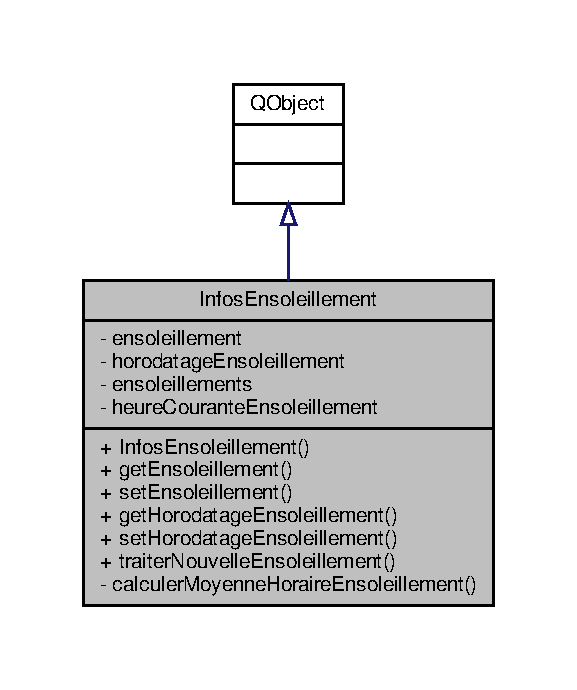
\includegraphics[width=277pt]{class_infos_ensoleillement__coll__graph}
\end{center}
\end{figure}
\subsubsection*{Connecteurs publics}
\begin{DoxyCompactItemize}
\item 
void \hyperlink{class_infos_ensoleillement_abe5426845614e3383e915dc9b3cacc3e}{traiter\+Nouvelle\+Ensoleillement} (Q\+String ensoleillement\+String, Q\+String \hyperlink{class_infos_ensoleillement_aa2014f9d13e69e9807543737240dbfd3}{horodatage\+Ensoleillement})
\begin{DoxyCompactList}\small\item\em slot qui traite l\textquotesingle{}ensoleillement \end{DoxyCompactList}\end{DoxyCompactItemize}
\subsubsection*{Signaux}
\begin{DoxyCompactItemize}
\item 
void \hyperlink{class_infos_ensoleillement_ac89935ebb118ba2d28504d7341f67a7f}{ensoleillement\+Envoye} (double \hyperlink{class_infos_ensoleillement_a5f3ad64743e3beeb4e64c4555ec6155c}{ensoleillement}, Q\+String horodatage)
\item 
void \hyperlink{class_infos_ensoleillement_a8c0f6c50648ffc4f47f049727e05e8d0}{traitement\+Ensoleillement\+Envoye} (double ensoleillement\+Moyen, double ensoleillement\+Minimum, double ensoleillement\+Maximum, int heure)
\end{DoxyCompactItemize}
\subsubsection*{Fonctions membres publiques}
\begin{DoxyCompactItemize}
\item 
\hyperlink{class_infos_ensoleillement_a5037621d40a4e62f01182f6742388fcd}{Infos\+Ensoleillement} (\hyperlink{class_q_object}{Q\+Object} $\ast$parent)
\begin{DoxyCompactList}\small\item\em Constructeur de la classe \hyperlink{class_infos_ensoleillement}{Infos\+Ensoleillement}. \end{DoxyCompactList}\item 
double \hyperlink{class_infos_ensoleillement_a388dd7b2ae97839a779ca1384ca8e6e2}{get\+Ensoleillement} ()
\begin{DoxyCompactList}\small\item\em getter de l\textquotesingle{}attribut ensoleillement \end{DoxyCompactList}\item 
void \hyperlink{class_infos_ensoleillement_a27c6d3d6e063e2f09fbe23a04cd89dfc}{set\+Ensoleillement} (double \hyperlink{class_infos_ensoleillement_a5f3ad64743e3beeb4e64c4555ec6155c}{ensoleillement})
\begin{DoxyCompactList}\small\item\em setter de l\textquotesingle{}attribut ensoleillement \end{DoxyCompactList}\item 
Q\+String \hyperlink{class_infos_ensoleillement_a0bd39540c8b4a242ea378c91bbc58b89}{get\+Horodatage\+Ensoleillement} () const
\begin{DoxyCompactList}\small\item\em getter de l\textquotesingle{}attibut horodatage\+Ensoleillement \end{DoxyCompactList}\item 
void \hyperlink{class_infos_ensoleillement_a35cd0359b8bcf5bd572cbef2195fa8d1}{set\+Horodatage\+Ensoleillement} (const Q\+String \hyperlink{class_infos_ensoleillement_aa2014f9d13e69e9807543737240dbfd3}{horodatage\+Ensoleillement})
\begin{DoxyCompactList}\small\item\em setter de l\textquotesingle{}attribut horodatage\+Ensoleillement \end{DoxyCompactList}\end{DoxyCompactItemize}
\subsubsection*{Fonctions membres privées}
\begin{DoxyCompactItemize}
\item 
void \hyperlink{class_infos_ensoleillement_a43d0967a59887bf70071296fef0660d3}{calculer\+Moyenne\+Horaire\+Ensoleillement} ()
\end{DoxyCompactItemize}
\subsubsection*{Attributs privés}
\begin{DoxyCompactItemize}
\item 
double \hyperlink{class_infos_ensoleillement_a5f3ad64743e3beeb4e64c4555ec6155c}{ensoleillement}
\begin{DoxyCompactList}\small\item\em valeur courante de l\textquotesingle{}ensoleillement en w/m² \end{DoxyCompactList}\item 
Q\+String \hyperlink{class_infos_ensoleillement_aa2014f9d13e69e9807543737240dbfd3}{horodatage\+Ensoleillement}
\begin{DoxyCompactList}\small\item\em horodatage de la l\textquotesingle{}ensoleillement \end{DoxyCompactList}\item 
Q\+Vector$<$ double $>$ \hyperlink{class_infos_ensoleillement_a6c3640ed7f3169e6263dc04b0191f478}{ensoleillements}
\item 
int \hyperlink{class_infos_ensoleillement_adbf40d147f8a7dbcf5f71b1ac4e0933d}{heure\+Courante\+Ensoleillement}
\end{DoxyCompactItemize}


\subsubsection{Description détaillée}
\begin{DoxyAuthor}{Auteur}
Florentin Mellah, Enzo Rossi
\end{DoxyAuthor}
\begin{DoxyVersion}{Version}
1.\+1 
\end{DoxyVersion}


\subsubsection{Documentation des constructeurs et destructeur}
\mbox{\Hypertarget{class_infos_ensoleillement_a5037621d40a4e62f01182f6742388fcd}\label{class_infos_ensoleillement_a5037621d40a4e62f01182f6742388fcd}} 
\index{Infos\+Ensoleillement@{Infos\+Ensoleillement}!Infos\+Ensoleillement@{Infos\+Ensoleillement}}
\index{Infos\+Ensoleillement@{Infos\+Ensoleillement}!Infos\+Ensoleillement@{Infos\+Ensoleillement}}
\paragraph{\texorpdfstring{Infos\+Ensoleillement()}{InfosEnsoleillement()}}
{\footnotesize\ttfamily Infos\+Ensoleillement\+::\+Infos\+Ensoleillement (\begin{DoxyParamCaption}\item[{\hyperlink{class_q_object}{Q\+Object} $\ast$}]{parent }\end{DoxyParamCaption})}

Définition des attributs ensoleillement à 0 et l\textquotesingle{}attribut horodatage\+Ensoleillement à \char`\"{}\char`\"{} 
\begin{DoxyCode}
00026                                                         :\hyperlink{class_q_object}{QObject}(parent), 
      \hyperlink{class_infos_ensoleillement_a5f3ad64743e3beeb4e64c4555ec6155c}{ensoleillement}(0.), \hyperlink{class_infos_ensoleillement_aa2014f9d13e69e9807543737240dbfd3}{horodatageEnsoleillement}(\textcolor{stringliteral}{""}), 
      \hyperlink{class_infos_ensoleillement_adbf40d147f8a7dbcf5f71b1ac4e0933d}{heureCouranteEnsoleillement}(-1)
00027 \{
00028 \}
\end{DoxyCode}


\subsubsection{Documentation des fonctions membres}
\mbox{\Hypertarget{class_infos_ensoleillement_a43d0967a59887bf70071296fef0660d3}\label{class_infos_ensoleillement_a43d0967a59887bf70071296fef0660d3}} 
\index{Infos\+Ensoleillement@{Infos\+Ensoleillement}!calculer\+Moyenne\+Horaire\+Ensoleillement@{calculer\+Moyenne\+Horaire\+Ensoleillement}}
\index{calculer\+Moyenne\+Horaire\+Ensoleillement@{calculer\+Moyenne\+Horaire\+Ensoleillement}!Infos\+Ensoleillement@{Infos\+Ensoleillement}}
\paragraph{\texorpdfstring{calculer\+Moyenne\+Horaire\+Ensoleillement()}{calculerMoyenneHoraireEnsoleillement()}}
{\footnotesize\ttfamily void Infos\+Ensoleillement\+::calculer\+Moyenne\+Horaire\+Ensoleillement (\begin{DoxyParamCaption}{ }\end{DoxyParamCaption})\hspace{0.3cm}{\ttfamily [private]}}



Références \hyperlink{class_infos_ensoleillement_a6c3640ed7f3169e6263dc04b0191f478}{ensoleillements}, \hyperlink{class_infos_ensoleillement_adbf40d147f8a7dbcf5f71b1ac4e0933d}{heure\+Courante\+Ensoleillement}, et \hyperlink{class_infos_ensoleillement_a8c0f6c50648ffc4f47f049727e05e8d0}{traitement\+Ensoleillement\+Envoye()}.



Référencé par \hyperlink{class_infos_ensoleillement_abe5426845614e3383e915dc9b3cacc3e}{traiter\+Nouvelle\+Ensoleillement()}.


\begin{DoxyCode}
00106 \{
00107     \textcolor{keywordtype}{double} sommeEnsoleillement= 0;
00108     \textcolor{keywordtype}{double} ensoleillementMoyen = 0;
00109     \textcolor{keywordtype}{double} ensoleillementMinimum = 999;
00110     \textcolor{keywordtype}{double} ensoleillementMaximum = -999;
00111 
00112     \textcolor{comment}{// au moins 2 mesures}
00113     \textcolor{keywordflow}{if}(\hyperlink{class_infos_ensoleillement_a6c3640ed7f3169e6263dc04b0191f478}{ensoleillements}.size() >= 2)
00114     \{
00115         ensoleillementMinimum = \hyperlink{class_infos_ensoleillement_a6c3640ed7f3169e6263dc04b0191f478}{ensoleillements}[0];
00116         ensoleillementMaximum = \hyperlink{class_infos_ensoleillement_a6c3640ed7f3169e6263dc04b0191f478}{ensoleillements}[0];
00117         \textcolor{keywordflow}{for} (\textcolor{keywordtype}{int} i = 0; i < \hyperlink{class_infos_ensoleillement_a6c3640ed7f3169e6263dc04b0191f478}{ensoleillements}.size(); i++)
00118         \{
00119             sommeEnsoleillement += \hyperlink{class_infos_ensoleillement_a6c3640ed7f3169e6263dc04b0191f478}{ensoleillements}[i];
00120 
00121             \textcolor{keywordflow}{if}(ensoleillementMinimum > \hyperlink{class_infos_ensoleillement_a6c3640ed7f3169e6263dc04b0191f478}{ensoleillements}[i])
00122             \{
00123                 ensoleillementMinimum = \hyperlink{class_infos_ensoleillement_a6c3640ed7f3169e6263dc04b0191f478}{ensoleillements}[i];
00124             \}
00125 
00126             \textcolor{keywordflow}{if}(ensoleillementMaximum < \hyperlink{class_infos_ensoleillement_a6c3640ed7f3169e6263dc04b0191f478}{ensoleillements}[i])
00127             \{
00128                 ensoleillementMaximum = \hyperlink{class_infos_ensoleillement_a6c3640ed7f3169e6263dc04b0191f478}{ensoleillements}[i];
00129             \}
00130         \}
00131     \}
00132     qDebug() << Q\_FUNC\_INFO << \hyperlink{class_infos_ensoleillement_a6c3640ed7f3169e6263dc04b0191f478}{ensoleillements};
00133     ensoleillementMoyen = sommeEnsoleillement/ double(ensoleillements.size());
00134     emit \hyperlink{class_infos_ensoleillement_a8c0f6c50648ffc4f47f049727e05e8d0}{traitementEnsoleillementEnvoye}(ensoleillementMoyen, 
      ensoleillementMinimum ,ensoleillementMaximum, \hyperlink{class_infos_ensoleillement_adbf40d147f8a7dbcf5f71b1ac4e0933d}{heureCouranteEnsoleillement});
00135     ensoleillements.clear();
00136 \}
\end{DoxyCode}
\mbox{\Hypertarget{class_infos_ensoleillement_ac89935ebb118ba2d28504d7341f67a7f}\label{class_infos_ensoleillement_ac89935ebb118ba2d28504d7341f67a7f}} 
\index{Infos\+Ensoleillement@{Infos\+Ensoleillement}!ensoleillement\+Envoye@{ensoleillement\+Envoye}}
\index{ensoleillement\+Envoye@{ensoleillement\+Envoye}!Infos\+Ensoleillement@{Infos\+Ensoleillement}}
\paragraph{\texorpdfstring{ensoleillement\+Envoye}{ensoleillementEnvoye}}
{\footnotesize\ttfamily void Infos\+Ensoleillement\+::ensoleillement\+Envoye (\begin{DoxyParamCaption}\item[{double}]{ensoleillement,  }\item[{Q\+String}]{horodatage }\end{DoxyParamCaption})\hspace{0.3cm}{\ttfamily [signal]}}



Référencé par \hyperlink{class_infos_ensoleillement_abe5426845614e3383e915dc9b3cacc3e}{traiter\+Nouvelle\+Ensoleillement()}.

\mbox{\Hypertarget{class_infos_ensoleillement_a388dd7b2ae97839a779ca1384ca8e6e2}\label{class_infos_ensoleillement_a388dd7b2ae97839a779ca1384ca8e6e2}} 
\index{Infos\+Ensoleillement@{Infos\+Ensoleillement}!get\+Ensoleillement@{get\+Ensoleillement}}
\index{get\+Ensoleillement@{get\+Ensoleillement}!Infos\+Ensoleillement@{Infos\+Ensoleillement}}
\paragraph{\texorpdfstring{get\+Ensoleillement()}{getEnsoleillement()}}
{\footnotesize\ttfamily double Infos\+Ensoleillement\+::get\+Ensoleillement (\begin{DoxyParamCaption}{ }\end{DoxyParamCaption})}

\begin{DoxyReturn}{Renvoie}
un {\itshape double} correspondant à la valeur de l\textquotesingle{}attibut ensoleillement 
\end{DoxyReturn}


Références \hyperlink{class_infos_ensoleillement_a5f3ad64743e3beeb4e64c4555ec6155c}{ensoleillement}.



Référencé par \hyperlink{class_alertes_ae7ad960c530a6a7e82df3ed55d159a68}{Alertes\+::alertes\+Ensoleillement()}.


\begin{DoxyCode}
00037 \{
00038     \textcolor{keywordflow}{return} \hyperlink{class_infos_ensoleillement_a5f3ad64743e3beeb4e64c4555ec6155c}{ensoleillement};
00039 \}
\end{DoxyCode}
\mbox{\Hypertarget{class_infos_ensoleillement_a0bd39540c8b4a242ea378c91bbc58b89}\label{class_infos_ensoleillement_a0bd39540c8b4a242ea378c91bbc58b89}} 
\index{Infos\+Ensoleillement@{Infos\+Ensoleillement}!get\+Horodatage\+Ensoleillement@{get\+Horodatage\+Ensoleillement}}
\index{get\+Horodatage\+Ensoleillement@{get\+Horodatage\+Ensoleillement}!Infos\+Ensoleillement@{Infos\+Ensoleillement}}
\paragraph{\texorpdfstring{get\+Horodatage\+Ensoleillement()}{getHorodatageEnsoleillement()}}
{\footnotesize\ttfamily Q\+String Infos\+Ensoleillement\+::get\+Horodatage\+Ensoleillement (\begin{DoxyParamCaption}{ }\end{DoxyParamCaption}) const}

\begin{DoxyReturn}{Renvoie}
un Q\+String correspondant a la valeur de l\textquotesingle{}attribut horodatage\+Ensoleillement 
\end{DoxyReturn}


Références \hyperlink{class_infos_ensoleillement_aa2014f9d13e69e9807543737240dbfd3}{horodatage\+Ensoleillement}.



Référencé par \hyperlink{class_ruche_ad21de5f7d48195be0658f52c55f34183}{Ruche\+::inserer\+Donnees\+Port\+Ensoleillement()}.


\begin{DoxyCode}
00059 \{
00060     \textcolor{keywordflow}{return} \hyperlink{class_infos_ensoleillement_aa2014f9d13e69e9807543737240dbfd3}{horodatageEnsoleillement};
00061 \}
\end{DoxyCode}
\mbox{\Hypertarget{class_infos_ensoleillement_a27c6d3d6e063e2f09fbe23a04cd89dfc}\label{class_infos_ensoleillement_a27c6d3d6e063e2f09fbe23a04cd89dfc}} 
\index{Infos\+Ensoleillement@{Infos\+Ensoleillement}!set\+Ensoleillement@{set\+Ensoleillement}}
\index{set\+Ensoleillement@{set\+Ensoleillement}!Infos\+Ensoleillement@{Infos\+Ensoleillement}}
\paragraph{\texorpdfstring{set\+Ensoleillement()}{setEnsoleillement()}}
{\footnotesize\ttfamily void Infos\+Ensoleillement\+::set\+Ensoleillement (\begin{DoxyParamCaption}\item[{double}]{ensoleillement }\end{DoxyParamCaption})}


\begin{DoxyParams}{Paramètres}
{\em ensoleillement} & \\
\hline
\end{DoxyParams}


Références \hyperlink{class_infos_ensoleillement_a5f3ad64743e3beeb4e64c4555ec6155c}{ensoleillement}.


\begin{DoxyCode}
00048 \{
00049     this->\hyperlink{class_infos_ensoleillement_a5f3ad64743e3beeb4e64c4555ec6155c}{ensoleillement} = \hyperlink{class_infos_ensoleillement_a5f3ad64743e3beeb4e64c4555ec6155c}{ensoleillement};
00050 \}
\end{DoxyCode}
\mbox{\Hypertarget{class_infos_ensoleillement_a35cd0359b8bcf5bd572cbef2195fa8d1}\label{class_infos_ensoleillement_a35cd0359b8bcf5bd572cbef2195fa8d1}} 
\index{Infos\+Ensoleillement@{Infos\+Ensoleillement}!set\+Horodatage\+Ensoleillement@{set\+Horodatage\+Ensoleillement}}
\index{set\+Horodatage\+Ensoleillement@{set\+Horodatage\+Ensoleillement}!Infos\+Ensoleillement@{Infos\+Ensoleillement}}
\paragraph{\texorpdfstring{set\+Horodatage\+Ensoleillement()}{setHorodatageEnsoleillement()}}
{\footnotesize\ttfamily void Infos\+Ensoleillement\+::set\+Horodatage\+Ensoleillement (\begin{DoxyParamCaption}\item[{const Q\+String}]{horodatage\+Ensoleillement }\end{DoxyParamCaption})}


\begin{DoxyParams}{Paramètres}
{\em horodatage\+Ensoleillement} & \\
\hline
\end{DoxyParams}


Références \hyperlink{class_infos_ensoleillement_aa2014f9d13e69e9807543737240dbfd3}{horodatage\+Ensoleillement}.


\begin{DoxyCode}
00070 \{
00071     this->\hyperlink{class_infos_ensoleillement_aa2014f9d13e69e9807543737240dbfd3}{horodatageEnsoleillement} = 
      \hyperlink{class_infos_ensoleillement_aa2014f9d13e69e9807543737240dbfd3}{horodatageEnsoleillement};
00072 \}
\end{DoxyCode}
\mbox{\Hypertarget{class_infos_ensoleillement_a8c0f6c50648ffc4f47f049727e05e8d0}\label{class_infos_ensoleillement_a8c0f6c50648ffc4f47f049727e05e8d0}} 
\index{Infos\+Ensoleillement@{Infos\+Ensoleillement}!traitement\+Ensoleillement\+Envoye@{traitement\+Ensoleillement\+Envoye}}
\index{traitement\+Ensoleillement\+Envoye@{traitement\+Ensoleillement\+Envoye}!Infos\+Ensoleillement@{Infos\+Ensoleillement}}
\paragraph{\texorpdfstring{traitement\+Ensoleillement\+Envoye}{traitementEnsoleillementEnvoye}}
{\footnotesize\ttfamily void Infos\+Ensoleillement\+::traitement\+Ensoleillement\+Envoye (\begin{DoxyParamCaption}\item[{double}]{ensoleillement\+Moyen,  }\item[{double}]{ensoleillement\+Minimum,  }\item[{double}]{ensoleillement\+Maximum,  }\item[{int}]{heure }\end{DoxyParamCaption})\hspace{0.3cm}{\ttfamily [signal]}}



Référencé par \hyperlink{class_infos_ensoleillement_a43d0967a59887bf70071296fef0660d3}{calculer\+Moyenne\+Horaire\+Ensoleillement()}.

\mbox{\Hypertarget{class_infos_ensoleillement_abe5426845614e3383e915dc9b3cacc3e}\label{class_infos_ensoleillement_abe5426845614e3383e915dc9b3cacc3e}} 
\index{Infos\+Ensoleillement@{Infos\+Ensoleillement}!traiter\+Nouvelle\+Ensoleillement@{traiter\+Nouvelle\+Ensoleillement}}
\index{traiter\+Nouvelle\+Ensoleillement@{traiter\+Nouvelle\+Ensoleillement}!Infos\+Ensoleillement@{Infos\+Ensoleillement}}
\paragraph{\texorpdfstring{traiter\+Nouvelle\+Ensoleillement}{traiterNouvelleEnsoleillement}}
{\footnotesize\ttfamily void Infos\+Ensoleillement\+::traiter\+Nouvelle\+Ensoleillement (\begin{DoxyParamCaption}\item[{Q\+String}]{ensoleillement\+String,  }\item[{Q\+String}]{horodatage\+Ensoleillement }\end{DoxyParamCaption})\hspace{0.3cm}{\ttfamily [slot]}}


\begin{DoxyParams}{Paramètres}
{\em ensoleillement\+String} & qui corespond a l\textquotesingle{}ensoleillement envoyé par la \hyperlink{class_ruche}{Ruche} \\
\hline
{\em horodatage\+Ensoleillement} & correspond a l\textquotesingle{}horodatage de la mesure de l\textquotesingle{}ensoleillement \\
\hline
\end{DoxyParams}


Références \hyperlink{class_infos_ensoleillement_a43d0967a59887bf70071296fef0660d3}{calculer\+Moyenne\+Horaire\+Ensoleillement()}, \hyperlink{class_infos_ensoleillement_a5f3ad64743e3beeb4e64c4555ec6155c}{ensoleillement}, \hyperlink{class_infos_ensoleillement_ac89935ebb118ba2d28504d7341f67a7f}{ensoleillement\+Envoye()}, \hyperlink{class_infos_ensoleillement_a6c3640ed7f3169e6263dc04b0191f478}{ensoleillements}, \hyperlink{class_infos_ensoleillement_adbf40d147f8a7dbcf5f71b1ac4e0933d}{heure\+Courante\+Ensoleillement}, et \hyperlink{class_infos_ensoleillement_aa2014f9d13e69e9807543737240dbfd3}{horodatage\+Ensoleillement}.


\begin{DoxyCode}
00082 \{
00083     \hyperlink{class_infos_ensoleillement_a5f3ad64743e3beeb4e64c4555ec6155c}{ensoleillement} = ensoleillementString.toDouble();
00084     this->\hyperlink{class_infos_ensoleillement_aa2014f9d13e69e9807543737240dbfd3}{horodatageEnsoleillement} = 
      \hyperlink{class_infos_ensoleillement_aa2014f9d13e69e9807543737240dbfd3}{horodatageEnsoleillement};
00085     emit \hyperlink{class_infos_ensoleillement_ac89935ebb118ba2d28504d7341f67a7f}{ensoleillementEnvoye}(\hyperlink{class_infos_ensoleillement_a5f3ad64743e3beeb4e64c4555ec6155c}{ensoleillement},
      \hyperlink{class_infos_ensoleillement_aa2014f9d13e69e9807543737240dbfd3}{horodatageEnsoleillement});
00086 
00087     QDateTime dateTimeHorodatage = QDateTime::fromString(
      \hyperlink{class_infos_ensoleillement_aa2014f9d13e69e9807543737240dbfd3}{horodatageEnsoleillement}, \textcolor{stringliteral}{"dd/MM/yyyy HH:mm:ss"});
00088     qDebug() << Q\_FUNC\_INFO << \textcolor{stringliteral}{"heureCouranteEnsoleillement"} << 
      \hyperlink{class_infos_ensoleillement_adbf40d147f8a7dbcf5f71b1ac4e0933d}{heureCouranteEnsoleillement} << dateTimeHorodatage.time().hour();
00089     \textcolor{keywordflow}{if}(\hyperlink{class_infos_ensoleillement_adbf40d147f8a7dbcf5f71b1ac4e0933d}{heureCouranteEnsoleillement} == -1)
00090     \{
00091         \hyperlink{class_infos_ensoleillement_adbf40d147f8a7dbcf5f71b1ac4e0933d}{heureCouranteEnsoleillement} = dateTimeHorodatage.time().hour();
00092     \}
00093     \textcolor{keywordflow}{if}(\hyperlink{class_infos_ensoleillement_adbf40d147f8a7dbcf5f71b1ac4e0933d}{heureCouranteEnsoleillement} == dateTimeHorodatage.time().hour())
00094     \{
00095         \hyperlink{class_infos_ensoleillement_a6c3640ed7f3169e6263dc04b0191f478}{ensoleillements}.append(\hyperlink{class_infos_ensoleillement_a5f3ad64743e3beeb4e64c4555ec6155c}{ensoleillement});
00096     \}
00097     \textcolor{keywordflow}{else} \textcolor{keywordflow}{if}((\hyperlink{class_infos_ensoleillement_adbf40d147f8a7dbcf5f71b1ac4e0933d}{heureCouranteEnsoleillement}+1)%24 == dateTimeHorodatage.time().hour
      ())
00098     \{
00099         \hyperlink{class_infos_ensoleillement_a43d0967a59887bf70071296fef0660d3}{calculerMoyenneHoraireEnsoleillement}();
00100         \hyperlink{class_infos_ensoleillement_adbf40d147f8a7dbcf5f71b1ac4e0933d}{heureCouranteEnsoleillement} = dateTimeHorodatage.time().hour();
00101         \hyperlink{class_infos_ensoleillement_a6c3640ed7f3169e6263dc04b0191f478}{ensoleillements}.append(\hyperlink{class_infos_ensoleillement_a5f3ad64743e3beeb4e64c4555ec6155c}{ensoleillement});
00102     \}
00103 \}
\end{DoxyCode}


\subsubsection{Documentation des données membres}
\mbox{\Hypertarget{class_infos_ensoleillement_a5f3ad64743e3beeb4e64c4555ec6155c}\label{class_infos_ensoleillement_a5f3ad64743e3beeb4e64c4555ec6155c}} 
\index{Infos\+Ensoleillement@{Infos\+Ensoleillement}!ensoleillement@{ensoleillement}}
\index{ensoleillement@{ensoleillement}!Infos\+Ensoleillement@{Infos\+Ensoleillement}}
\paragraph{\texorpdfstring{ensoleillement}{ensoleillement}}
{\footnotesize\ttfamily double Infos\+Ensoleillement\+::ensoleillement\hspace{0.3cm}{\ttfamily [private]}}



Référencé par \hyperlink{class_infos_ensoleillement_a388dd7b2ae97839a779ca1384ca8e6e2}{get\+Ensoleillement()}, \hyperlink{class_infos_ensoleillement_a27c6d3d6e063e2f09fbe23a04cd89dfc}{set\+Ensoleillement()}, et \hyperlink{class_infos_ensoleillement_abe5426845614e3383e915dc9b3cacc3e}{traiter\+Nouvelle\+Ensoleillement()}.

\mbox{\Hypertarget{class_infos_ensoleillement_a6c3640ed7f3169e6263dc04b0191f478}\label{class_infos_ensoleillement_a6c3640ed7f3169e6263dc04b0191f478}} 
\index{Infos\+Ensoleillement@{Infos\+Ensoleillement}!ensoleillements@{ensoleillements}}
\index{ensoleillements@{ensoleillements}!Infos\+Ensoleillement@{Infos\+Ensoleillement}}
\paragraph{\texorpdfstring{ensoleillements}{ensoleillements}}
{\footnotesize\ttfamily Q\+Vector$<$double$>$ Infos\+Ensoleillement\+::ensoleillements\hspace{0.3cm}{\ttfamily [private]}}



Référencé par \hyperlink{class_infos_ensoleillement_a43d0967a59887bf70071296fef0660d3}{calculer\+Moyenne\+Horaire\+Ensoleillement()}, et \hyperlink{class_infos_ensoleillement_abe5426845614e3383e915dc9b3cacc3e}{traiter\+Nouvelle\+Ensoleillement()}.

\mbox{\Hypertarget{class_infos_ensoleillement_adbf40d147f8a7dbcf5f71b1ac4e0933d}\label{class_infos_ensoleillement_adbf40d147f8a7dbcf5f71b1ac4e0933d}} 
\index{Infos\+Ensoleillement@{Infos\+Ensoleillement}!heure\+Courante\+Ensoleillement@{heure\+Courante\+Ensoleillement}}
\index{heure\+Courante\+Ensoleillement@{heure\+Courante\+Ensoleillement}!Infos\+Ensoleillement@{Infos\+Ensoleillement}}
\paragraph{\texorpdfstring{heure\+Courante\+Ensoleillement}{heureCouranteEnsoleillement}}
{\footnotesize\ttfamily int Infos\+Ensoleillement\+::heure\+Courante\+Ensoleillement\hspace{0.3cm}{\ttfamily [private]}}



Référencé par \hyperlink{class_infos_ensoleillement_a43d0967a59887bf70071296fef0660d3}{calculer\+Moyenne\+Horaire\+Ensoleillement()}, et \hyperlink{class_infos_ensoleillement_abe5426845614e3383e915dc9b3cacc3e}{traiter\+Nouvelle\+Ensoleillement()}.

\mbox{\Hypertarget{class_infos_ensoleillement_aa2014f9d13e69e9807543737240dbfd3}\label{class_infos_ensoleillement_aa2014f9d13e69e9807543737240dbfd3}} 
\index{Infos\+Ensoleillement@{Infos\+Ensoleillement}!horodatage\+Ensoleillement@{horodatage\+Ensoleillement}}
\index{horodatage\+Ensoleillement@{horodatage\+Ensoleillement}!Infos\+Ensoleillement@{Infos\+Ensoleillement}}
\paragraph{\texorpdfstring{horodatage\+Ensoleillement}{horodatageEnsoleillement}}
{\footnotesize\ttfamily Q\+String Infos\+Ensoleillement\+::horodatage\+Ensoleillement\hspace{0.3cm}{\ttfamily [private]}}



Référencé par \hyperlink{class_infos_ensoleillement_a0bd39540c8b4a242ea378c91bbc58b89}{get\+Horodatage\+Ensoleillement()}, \hyperlink{class_infos_ensoleillement_a35cd0359b8bcf5bd572cbef2195fa8d1}{set\+Horodatage\+Ensoleillement()}, et \hyperlink{class_infos_ensoleillement_abe5426845614e3383e915dc9b3cacc3e}{traiter\+Nouvelle\+Ensoleillement()}.



La documentation de cette classe a été générée à partir des fichiers suivants \+:\begin{DoxyCompactItemize}
\item 
\hyperlink{infos_ensoleillement_8h}{infos\+Ensoleillement.\+h}\item 
\hyperlink{infos_ensoleillement_8cpp}{infos\+Ensoleillement.\+cpp}\end{DoxyCompactItemize}

\hypertarget{class_infos_humidite}{}\subsection{Référence de la classe Infos\+Humidite}
\label{class_infos_humidite}\index{Infos\+Humidite@{Infos\+Humidite}}


La classe \hyperlink{class_infos_humidite}{Infos\+Humidite}.  




{\ttfamily \#include $<$infos\+Humidite.\+h$>$}



Graphe de collaboration de Infos\+Humidite\+:\nopagebreak
\begin{figure}[H]
\begin{center}
\leavevmode
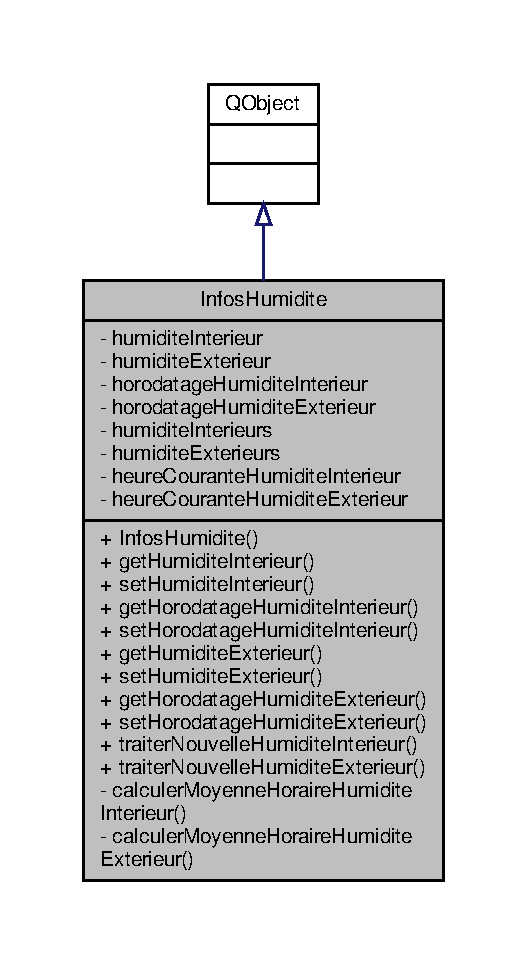
\includegraphics[width=253pt]{class_infos_humidite__coll__graph}
\end{center}
\end{figure}
\subsubsection*{Connecteurs publics}
\begin{DoxyCompactItemize}
\item 
void \hyperlink{class_infos_humidite_a0995d68a036f73df3b5a86e5538104bd}{traiter\+Nouvelle\+Humidite\+Interieur} (Q\+String humidite\+Interieurstring, Q\+String \hyperlink{class_infos_humidite_a38712bac5a2d4d106a016647ad39fedf}{horodatage\+Humidite\+Interieur})
\begin{DoxyCompactList}\small\item\em slot qui traite l\textquotesingle{}humidite Interieur \end{DoxyCompactList}\item 
void \hyperlink{class_infos_humidite_a8d17fa3c7d15b1ff8130ae5d22702e5f}{traiter\+Nouvelle\+Humidite\+Exterieur} (Q\+String humidite\+Exterieurstring, Q\+String \hyperlink{class_infos_humidite_aa08b4f342e83f8ad437a8272698bb512}{horodatage\+Humidite\+Exterieur})
\begin{DoxyCompactList}\small\item\em slot qui traite l\textquotesingle{}humidite Exterieur \end{DoxyCompactList}\end{DoxyCompactItemize}
\subsubsection*{Signaux}
\begin{DoxyCompactItemize}
\item 
void \hyperlink{class_infos_humidite_aa0eb7d8a609b837e1b450b7d79e1ff81}{humidite\+Interieur\+Envoye} (const double \hyperlink{class_infos_humidite_ad2847e671ad0b90f8dc0940dee107c38}{humidite\+Interieur}, Q\+String horodatage)
\begin{DoxyCompactList}\small\item\em signal vers la classe \hyperlink{class_ruche}{Ruche} \end{DoxyCompactList}\item 
void \hyperlink{class_infos_humidite_a666d4bd12639460ea0fd2a3f483c2842}{humidite\+Exterieur\+Envoye} (const double \hyperlink{class_infos_humidite_a503a9c849508928d3046292f17f37230}{humidite\+Exterieur}, Q\+String horodatage)
\item 
void \hyperlink{class_infos_humidite_a3643afa07ff3ac73a4190d77ce230d3b}{traitement\+Humidite\+Interieur\+Envoye} (const double temperature\+Interieur\+Moyenne, const double temperature\+Interieur\+Minimum, const double temperature\+Interieur\+Maximum, int heure)
\item 
void \hyperlink{class_infos_humidite_abd0535dee74a4588232d282d0fe64829}{traitement\+Humidite\+Exterieur\+Envoye} (const double temperature\+Exterieur\+Moyenne, const double temperature\+Exterieur\+Minimum, const double temperature\+Exterieur\+Maximum, int heure)
\end{DoxyCompactItemize}
\subsubsection*{Fonctions membres publiques}
\begin{DoxyCompactItemize}
\item 
\hyperlink{class_infos_humidite_a3c87ffa0e896fd5af90b1d9f15a47a57}{Infos\+Humidite} (\hyperlink{class_q_object}{Q\+Object} $\ast$parent)
\begin{DoxyCompactList}\small\item\em Constructeur de la classe \hyperlink{class_infos_humidite}{Infos\+Humidite}. \end{DoxyCompactList}\item 
double \hyperlink{class_infos_humidite_a652f7ca3e4b97352034fed62c6d865b7}{get\+Humidite\+Interieur} ()
\begin{DoxyCompactList}\small\item\em getter de l\textquotesingle{}attribut humidite\+Interieur \end{DoxyCompactList}\item 
void \hyperlink{class_infos_humidite_a238c8b3bd6b09c4f770058a05468baa8}{set\+Humidite\+Interieur} (double \hyperlink{class_infos_humidite_ad2847e671ad0b90f8dc0940dee107c38}{humidite\+Interieur})
\begin{DoxyCompactList}\small\item\em setter de l\textquotesingle{}attribut humidite\+Interieur \end{DoxyCompactList}\item 
Q\+String \hyperlink{class_infos_humidite_a841d2583f206a9097fa3871adc8be568}{get\+Horodatage\+Humidite\+Interieur} () const
\begin{DoxyCompactList}\small\item\em getter de l\textquotesingle{}attribut horodatage\+Humidite\+Interieur \end{DoxyCompactList}\item 
void \hyperlink{class_infos_humidite_a8054d13ab8f57504392756351c376534}{set\+Horodatage\+Humidite\+Interieur} (const Q\+String \hyperlink{class_infos_humidite_a38712bac5a2d4d106a016647ad39fedf}{horodatage\+Humidite\+Interieur})
\begin{DoxyCompactList}\small\item\em \hyperlink{class_infos_humidite_a8054d13ab8f57504392756351c376534}{Infos\+Humidite\+::set\+Horodatage\+Humidite\+Interieur}. \end{DoxyCompactList}\item 
double \hyperlink{class_infos_humidite_a23e537fdfa33336a3970838f445387ce}{get\+Humidite\+Exterieur} ()
\begin{DoxyCompactList}\small\item\em getter de l\textquotesingle{}attribut humidite\+Exterieur \end{DoxyCompactList}\item 
void \hyperlink{class_infos_humidite_a8228ff1f1d0466df228ed3f2e2d269ac}{set\+Humidite\+Exterieur} (double \hyperlink{class_infos_humidite_a503a9c849508928d3046292f17f37230}{humidite\+Exterieur})
\begin{DoxyCompactList}\small\item\em setter de l\textquotesingle{}attribut humidite\+Exterieur \end{DoxyCompactList}\item 
Q\+String \hyperlink{class_infos_humidite_a04abb2841492704e125874464052bb4f}{get\+Horodatage\+Humidite\+Exterieur} () const
\begin{DoxyCompactList}\small\item\em getter de l\textquotesingle{}attribut horodatage\+Humidite\+Exterieur \end{DoxyCompactList}\item 
void \hyperlink{class_infos_humidite_acc6231789bd923840dadf4f17310ce69}{set\+Horodatage\+Humidite\+Exterieur} (const Q\+String \hyperlink{class_infos_humidite_aa08b4f342e83f8ad437a8272698bb512}{horodatage\+Humidite\+Exterieur})
\begin{DoxyCompactList}\small\item\em setter de l\textquotesingle{}attribut horodatage\+Humidite\+Exterieur \end{DoxyCompactList}\end{DoxyCompactItemize}
\subsubsection*{Fonctions membres privées}
\begin{DoxyCompactItemize}
\item 
void \hyperlink{class_infos_humidite_acd903311f6c949f8f010b330f517e4f3}{calculer\+Moyenne\+Horaire\+Humidite\+Interieur} ()
\item 
void \hyperlink{class_infos_humidite_afc4f6ba3cd4664118ef40f4c12b76506}{calculer\+Moyenne\+Horaire\+Humidite\+Exterieur} ()
\end{DoxyCompactItemize}
\subsubsection*{Attributs privés}
\begin{DoxyCompactItemize}
\item 
double \hyperlink{class_infos_humidite_ad2847e671ad0b90f8dc0940dee107c38}{humidite\+Interieur}
\begin{DoxyCompactList}\small\item\em humidité interieur en pourcentage \end{DoxyCompactList}\item 
double \hyperlink{class_infos_humidite_a503a9c849508928d3046292f17f37230}{humidite\+Exterieur}
\begin{DoxyCompactList}\small\item\em humidité exterieur en pourcentage \end{DoxyCompactList}\item 
Q\+String \hyperlink{class_infos_humidite_a38712bac5a2d4d106a016647ad39fedf}{horodatage\+Humidite\+Interieur}
\begin{DoxyCompactList}\small\item\em horodatage de l\textquotesingle{}humidité interieur \end{DoxyCompactList}\item 
Q\+String \hyperlink{class_infos_humidite_aa08b4f342e83f8ad437a8272698bb512}{horodatage\+Humidite\+Exterieur}
\begin{DoxyCompactList}\small\item\em horodatage de l\textquotesingle{}humidité exterieur \end{DoxyCompactList}\item 
Q\+Vector$<$ double $>$ \hyperlink{class_infos_humidite_a2bcd5b3629a007078d4e15d110dae457}{humidite\+Interieurs}
\item 
Q\+Vector$<$ double $>$ \hyperlink{class_infos_humidite_a62d1331116ee1cf00cb8fa369a214c62}{humidite\+Exterieurs}
\item 
int \hyperlink{class_infos_humidite_a5a8597751ba0fe10a14a12e155421485}{heure\+Courante\+Humidite\+Interieur}
\item 
int \hyperlink{class_infos_humidite_ad7b450373a47ec831872872e0e5674ad}{heure\+Courante\+Humidite\+Exterieur}
\end{DoxyCompactItemize}


\subsubsection{Description détaillée}
\begin{DoxyAuthor}{Auteur}
Florentin Mellah, Enzo Rossi
\end{DoxyAuthor}
\begin{DoxyVersion}{Version}
1.\+1 
\end{DoxyVersion}


\subsubsection{Documentation des constructeurs et destructeur}
\mbox{\Hypertarget{class_infos_humidite_a3c87ffa0e896fd5af90b1d9f15a47a57}\label{class_infos_humidite_a3c87ffa0e896fd5af90b1d9f15a47a57}} 
\index{Infos\+Humidite@{Infos\+Humidite}!Infos\+Humidite@{Infos\+Humidite}}
\index{Infos\+Humidite@{Infos\+Humidite}!Infos\+Humidite@{Infos\+Humidite}}
\paragraph{\texorpdfstring{Infos\+Humidite()}{InfosHumidite()}}
{\footnotesize\ttfamily Infos\+Humidite\+::\+Infos\+Humidite (\begin{DoxyParamCaption}\item[{\hyperlink{class_q_object}{Q\+Object} $\ast$}]{parent }\end{DoxyParamCaption})}

Définition des attributs pression\+Atmospherique à 0 et l\textquotesingle{}attribut horodatage\+Pression\+Atmospherique à \char`\"{}\char`\"{} 
\begin{DoxyCode}
00026                                             :\hyperlink{class_q_object}{QObject}(parent),
      \hyperlink{class_infos_humidite_ad2847e671ad0b90f8dc0940dee107c38}{humiditeInterieur}(0),\hyperlink{class_infos_humidite_a503a9c849508928d3046292f17f37230}{humiditeExterieur}(0),
      \hyperlink{class_infos_humidite_a38712bac5a2d4d106a016647ad39fedf}{horodatageHumiditeInterieur}(\textcolor{stringliteral}{""}),
      \hyperlink{class_infos_humidite_aa08b4f342e83f8ad437a8272698bb512}{horodatageHumiditeExterieur}(\textcolor{stringliteral}{""}), 
      \hyperlink{class_infos_humidite_a5a8597751ba0fe10a14a12e155421485}{heureCouranteHumiditeInterieur}(-1), 
      \hyperlink{class_infos_humidite_ad7b450373a47ec831872872e0e5674ad}{heureCouranteHumiditeExterieur}(-1)
00027 \{
00028 \}
\end{DoxyCode}


\subsubsection{Documentation des fonctions membres}
\mbox{\Hypertarget{class_infos_humidite_afc4f6ba3cd4664118ef40f4c12b76506}\label{class_infos_humidite_afc4f6ba3cd4664118ef40f4c12b76506}} 
\index{Infos\+Humidite@{Infos\+Humidite}!calculer\+Moyenne\+Horaire\+Humidite\+Exterieur@{calculer\+Moyenne\+Horaire\+Humidite\+Exterieur}}
\index{calculer\+Moyenne\+Horaire\+Humidite\+Exterieur@{calculer\+Moyenne\+Horaire\+Humidite\+Exterieur}!Infos\+Humidite@{Infos\+Humidite}}
\paragraph{\texorpdfstring{calculer\+Moyenne\+Horaire\+Humidite\+Exterieur()}{calculerMoyenneHoraireHumiditeExterieur()}}
{\footnotesize\ttfamily void Infos\+Humidite\+::calculer\+Moyenne\+Horaire\+Humidite\+Exterieur (\begin{DoxyParamCaption}{ }\end{DoxyParamCaption})\hspace{0.3cm}{\ttfamily [private]}}



Références \hyperlink{class_infos_humidite_ad7b450373a47ec831872872e0e5674ad}{heure\+Courante\+Humidite\+Exterieur}, \hyperlink{class_infos_humidite_a62d1331116ee1cf00cb8fa369a214c62}{humidite\+Exterieurs}, et \hyperlink{class_infos_humidite_abd0535dee74a4588232d282d0fe64829}{traitement\+Humidite\+Exterieur\+Envoye()}.



Référencé par \hyperlink{class_infos_humidite_a8d17fa3c7d15b1ff8130ae5d22702e5f}{traiter\+Nouvelle\+Humidite\+Exterieur()}.


\begin{DoxyCode}
00215 \{
00216     \textcolor{keywordtype}{double} sommeHumiditeExterieur = 0;
00217     \textcolor{keywordtype}{double} humiditeExterieurMoyenne = 0;
00218     \textcolor{keywordtype}{double} humiditeExterieurMinimum = 999;
00219     \textcolor{keywordtype}{double} humiditeExterieurMaximum = -999;
00220 
00221     \textcolor{comment}{// au moins 2 mesures}
00222     \textcolor{keywordflow}{if}(\hyperlink{class_infos_humidite_a62d1331116ee1cf00cb8fa369a214c62}{humiditeExterieurs}.size() >= 2)
00223     \{
00224         humiditeExterieurMinimum = \hyperlink{class_infos_humidite_a62d1331116ee1cf00cb8fa369a214c62}{humiditeExterieurs}[0];
00225         humiditeExterieurMaximum = \hyperlink{class_infos_humidite_a62d1331116ee1cf00cb8fa369a214c62}{humiditeExterieurs}[0];
00226         \textcolor{keywordflow}{for} (\textcolor{keywordtype}{int} i = 0; i < \hyperlink{class_infos_humidite_a62d1331116ee1cf00cb8fa369a214c62}{humiditeExterieurs}.size(); i++)
00227         \{
00228             sommeHumiditeExterieur += \hyperlink{class_infos_humidite_a62d1331116ee1cf00cb8fa369a214c62}{humiditeExterieurs}[i];
00229 
00230             \textcolor{keywordflow}{if}(humiditeExterieurMinimum > \hyperlink{class_infos_humidite_a62d1331116ee1cf00cb8fa369a214c62}{humiditeExterieurs}[i])
00231             \{
00232                 humiditeExterieurMinimum = \hyperlink{class_infos_humidite_a62d1331116ee1cf00cb8fa369a214c62}{humiditeExterieurs}[i];
00233             \}
00234 
00235             \textcolor{keywordflow}{if}(humiditeExterieurMaximum < \hyperlink{class_infos_humidite_a62d1331116ee1cf00cb8fa369a214c62}{humiditeExterieurs}[i])
00236             \{
00237                 humiditeExterieurMaximum = \hyperlink{class_infos_humidite_a62d1331116ee1cf00cb8fa369a214c62}{humiditeExterieurs}[i];
00238             \}
00239         \}
00240     \}
00241     qDebug() << Q\_FUNC\_INFO << \hyperlink{class_infos_humidite_a62d1331116ee1cf00cb8fa369a214c62}{humiditeExterieurs};
00242     qDebug() << Q\_FUNC\_INFO << \textcolor{stringliteral}{"humiditeExterieurMoyenne="} << humiditeExterieurMoyenne << \textcolor{stringliteral}{"
      humiditeExterieurMinimum="} << humiditeExterieurMinimum << \textcolor{stringliteral}{"humiditeExterieurMaximum="} << humiditeExterieurMaximum;
00243     humiditeExterieurMoyenne = sommeHumiditeExterieur / double(humiditeExterieurs.size());
00244     emit \hyperlink{class_infos_humidite_abd0535dee74a4588232d282d0fe64829}{traitementHumiditeExterieurEnvoye}(humiditeExterieurMoyenne, 
      humiditeExterieurMinimum, humiditeExterieurMaximum, \hyperlink{class_infos_humidite_ad7b450373a47ec831872872e0e5674ad}{heureCouranteHumiditeExterieur})
      ;
00245     humiditeExterieurs.clear();
00246 \}
\end{DoxyCode}
\mbox{\Hypertarget{class_infos_humidite_acd903311f6c949f8f010b330f517e4f3}\label{class_infos_humidite_acd903311f6c949f8f010b330f517e4f3}} 
\index{Infos\+Humidite@{Infos\+Humidite}!calculer\+Moyenne\+Horaire\+Humidite\+Interieur@{calculer\+Moyenne\+Horaire\+Humidite\+Interieur}}
\index{calculer\+Moyenne\+Horaire\+Humidite\+Interieur@{calculer\+Moyenne\+Horaire\+Humidite\+Interieur}!Infos\+Humidite@{Infos\+Humidite}}
\paragraph{\texorpdfstring{calculer\+Moyenne\+Horaire\+Humidite\+Interieur()}{calculerMoyenneHoraireHumiditeInterieur()}}
{\footnotesize\ttfamily void Infos\+Humidite\+::calculer\+Moyenne\+Horaire\+Humidite\+Interieur (\begin{DoxyParamCaption}{ }\end{DoxyParamCaption})\hspace{0.3cm}{\ttfamily [private]}}



Références \hyperlink{class_infos_humidite_a5a8597751ba0fe10a14a12e155421485}{heure\+Courante\+Humidite\+Interieur}, \hyperlink{class_infos_humidite_a2bcd5b3629a007078d4e15d110dae457}{humidite\+Interieurs}, et \hyperlink{class_infos_humidite_a3643afa07ff3ac73a4190d77ce230d3b}{traitement\+Humidite\+Interieur\+Envoye()}.



Référencé par \hyperlink{class_infos_humidite_a0995d68a036f73df3b5a86e5538104bd}{traiter\+Nouvelle\+Humidite\+Interieur()}.


\begin{DoxyCode}
00176 \{
00177     \textcolor{keywordtype}{double} sommeHumiditeInterieur = 0;
00178     \textcolor{keywordtype}{double} humiditeInterieurMoyenne = 0;
00179     \textcolor{keywordtype}{double} humiditeInterieurMinimum = 999;
00180     \textcolor{keywordtype}{double} humiditeInterieurMaximum = -999;
00181 
00182     \textcolor{comment}{// au moins 2 mesures}
00183     \textcolor{keywordflow}{if}(\hyperlink{class_infos_humidite_a2bcd5b3629a007078d4e15d110dae457}{humiditeInterieurs}.size() >= 2)
00184     \{
00185         humiditeInterieurMinimum = \hyperlink{class_infos_humidite_a2bcd5b3629a007078d4e15d110dae457}{humiditeInterieurs}[0];
00186         humiditeInterieurMaximum = \hyperlink{class_infos_humidite_a2bcd5b3629a007078d4e15d110dae457}{humiditeInterieurs}[0];
00187         \textcolor{keywordflow}{for} (\textcolor{keywordtype}{int} i = 0; i < \hyperlink{class_infos_humidite_a2bcd5b3629a007078d4e15d110dae457}{humiditeInterieurs}.size(); i++)
00188         \{
00189             sommeHumiditeInterieur += \hyperlink{class_infos_humidite_a2bcd5b3629a007078d4e15d110dae457}{humiditeInterieurs}[i];
00190 
00191             \textcolor{keywordflow}{if}(humiditeInterieurMinimum > \hyperlink{class_infos_humidite_a2bcd5b3629a007078d4e15d110dae457}{humiditeInterieurs}[i])
00192             \{
00193                 humiditeInterieurMinimum = \hyperlink{class_infos_humidite_a2bcd5b3629a007078d4e15d110dae457}{humiditeInterieurs}[i];
00194             \}
00195 
00196             \textcolor{keywordflow}{if}(humiditeInterieurMaximum < \hyperlink{class_infos_humidite_a2bcd5b3629a007078d4e15d110dae457}{humiditeInterieurs}[i])
00197             \{
00198                 humiditeInterieurMaximum = \hyperlink{class_infos_humidite_a2bcd5b3629a007078d4e15d110dae457}{humiditeInterieurs}[i];
00199             \}
00200         \}
00201     \}
00202     qDebug() << Q\_FUNC\_INFO << \hyperlink{class_infos_humidite_a2bcd5b3629a007078d4e15d110dae457}{humiditeInterieurs};
00203     qDebug() << Q\_FUNC\_INFO << \textcolor{stringliteral}{"humiditeInterieurMoyenne="} << humiditeInterieurMoyenne << \textcolor{stringliteral}{"
      humiditeInterieurMinimum="} << humiditeInterieurMinimum << \textcolor{stringliteral}{"humiditeInterieurMaximum="} << humiditeInterieurMaximum;
00204     humiditeInterieurMoyenne = sommeHumiditeInterieur / double(humiditeInterieurs.size());
00205     emit \hyperlink{class_infos_humidite_a3643afa07ff3ac73a4190d77ce230d3b}{traitementHumiditeInterieurEnvoye}(humiditeInterieurMoyenne, 
      humiditeInterieurMinimum, humiditeInterieurMaximum, \hyperlink{class_infos_humidite_a5a8597751ba0fe10a14a12e155421485}{heureCouranteHumiditeInterieur})
      ;
00206     humiditeInterieurs.clear();
00207 \}
\end{DoxyCode}
\mbox{\Hypertarget{class_infos_humidite_a04abb2841492704e125874464052bb4f}\label{class_infos_humidite_a04abb2841492704e125874464052bb4f}} 
\index{Infos\+Humidite@{Infos\+Humidite}!get\+Horodatage\+Humidite\+Exterieur@{get\+Horodatage\+Humidite\+Exterieur}}
\index{get\+Horodatage\+Humidite\+Exterieur@{get\+Horodatage\+Humidite\+Exterieur}!Infos\+Humidite@{Infos\+Humidite}}
\paragraph{\texorpdfstring{get\+Horodatage\+Humidite\+Exterieur()}{getHorodatageHumiditeExterieur()}}
{\footnotesize\ttfamily Q\+String Infos\+Humidite\+::get\+Horodatage\+Humidite\+Exterieur (\begin{DoxyParamCaption}{ }\end{DoxyParamCaption}) const}

\begin{DoxyReturn}{Renvoie}
un {\itshape Q\+String} correspondant a la valeur de l\textquotesingle{}attribut horodatage\+Humidite\+Exterieur 
\end{DoxyReturn}


Références \hyperlink{class_infos_humidite_aa08b4f342e83f8ad437a8272698bb512}{horodatage\+Humidite\+Exterieur}.


\begin{DoxyCode}
00098 \{
00099     \textcolor{keywordflow}{return} \hyperlink{class_infos_humidite_aa08b4f342e83f8ad437a8272698bb512}{horodatageHumiditeExterieur};
00100 \}
\end{DoxyCode}
\mbox{\Hypertarget{class_infos_humidite_a841d2583f206a9097fa3871adc8be568}\label{class_infos_humidite_a841d2583f206a9097fa3871adc8be568}} 
\index{Infos\+Humidite@{Infos\+Humidite}!get\+Horodatage\+Humidite\+Interieur@{get\+Horodatage\+Humidite\+Interieur}}
\index{get\+Horodatage\+Humidite\+Interieur@{get\+Horodatage\+Humidite\+Interieur}!Infos\+Humidite@{Infos\+Humidite}}
\paragraph{\texorpdfstring{get\+Horodatage\+Humidite\+Interieur()}{getHorodatageHumiditeInterieur()}}
{\footnotesize\ttfamily Q\+String Infos\+Humidite\+::get\+Horodatage\+Humidite\+Interieur (\begin{DoxyParamCaption}{ }\end{DoxyParamCaption}) const}

\begin{DoxyReturn}{Renvoie}
{\itshape Q\+String} horodatage\+Humidite\+Interieur corespondant a l\textquotesingle{}attribut horodatage\+Humidite\+Interieur 
\end{DoxyReturn}


Références \hyperlink{class_infos_humidite_a38712bac5a2d4d106a016647ad39fedf}{horodatage\+Humidite\+Interieur}.


\begin{DoxyCode}
00057 \{
00058     \textcolor{keywordflow}{return} \hyperlink{class_infos_humidite_a38712bac5a2d4d106a016647ad39fedf}{horodatageHumiditeInterieur};
00059 \}
\end{DoxyCode}
\mbox{\Hypertarget{class_infos_humidite_a23e537fdfa33336a3970838f445387ce}\label{class_infos_humidite_a23e537fdfa33336a3970838f445387ce}} 
\index{Infos\+Humidite@{Infos\+Humidite}!get\+Humidite\+Exterieur@{get\+Humidite\+Exterieur}}
\index{get\+Humidite\+Exterieur@{get\+Humidite\+Exterieur}!Infos\+Humidite@{Infos\+Humidite}}
\paragraph{\texorpdfstring{get\+Humidite\+Exterieur()}{getHumiditeExterieur()}}
{\footnotesize\ttfamily double Infos\+Humidite\+::get\+Humidite\+Exterieur (\begin{DoxyParamCaption}{ }\end{DoxyParamCaption})}

\begin{DoxyReturn}{Renvoie}
{\itshape double} la valeur de l\textquotesingle{}humidite\+Exterieur 
\end{DoxyReturn}


Références \hyperlink{class_infos_humidite_a503a9c849508928d3046292f17f37230}{humidite\+Exterieur}.



Référencé par \hyperlink{class_alertes_a8606946eaa04dfd29bb7951b2b850a04}{Alertes\+::alertes\+Humidite\+Exterieur()}.


\begin{DoxyCode}
00077 \{
00078     \textcolor{keywordflow}{return} \hyperlink{class_infos_humidite_a503a9c849508928d3046292f17f37230}{humiditeExterieur};
00079 \}
\end{DoxyCode}
\mbox{\Hypertarget{class_infos_humidite_a652f7ca3e4b97352034fed62c6d865b7}\label{class_infos_humidite_a652f7ca3e4b97352034fed62c6d865b7}} 
\index{Infos\+Humidite@{Infos\+Humidite}!get\+Humidite\+Interieur@{get\+Humidite\+Interieur}}
\index{get\+Humidite\+Interieur@{get\+Humidite\+Interieur}!Infos\+Humidite@{Infos\+Humidite}}
\paragraph{\texorpdfstring{get\+Humidite\+Interieur()}{getHumiditeInterieur()}}
{\footnotesize\ttfamily double Infos\+Humidite\+::get\+Humidite\+Interieur (\begin{DoxyParamCaption}{ }\end{DoxyParamCaption})}

\begin{DoxyReturn}{Renvoie}
{\itshape double} corespondant a la valeur de l\textquotesingle{}attribut humidite\+Interieur 
\end{DoxyReturn}


Références \hyperlink{class_infos_humidite_ad2847e671ad0b90f8dc0940dee107c38}{humidite\+Interieur}.



Référencé par \hyperlink{class_alertes_a7558cb097dc392547ceb12ab4d6cbd4c}{Alertes\+::alertes\+Humidite\+Interieur()}, et \hyperlink{class_ruche_aa61f6dd8b15e5242ef3a3bdd87cca4a3}{Ruche\+::inserer\+Donnees\+Port\+Mesure\+Ruche()}.


\begin{DoxyCode}
00037 \{
00038     \textcolor{keywordflow}{return} \hyperlink{class_infos_humidite_ad2847e671ad0b90f8dc0940dee107c38}{humiditeInterieur};
00039 \}
\end{DoxyCode}
\mbox{\Hypertarget{class_infos_humidite_a666d4bd12639460ea0fd2a3f483c2842}\label{class_infos_humidite_a666d4bd12639460ea0fd2a3f483c2842}} 
\index{Infos\+Humidite@{Infos\+Humidite}!humidite\+Exterieur\+Envoye@{humidite\+Exterieur\+Envoye}}
\index{humidite\+Exterieur\+Envoye@{humidite\+Exterieur\+Envoye}!Infos\+Humidite@{Infos\+Humidite}}
\paragraph{\texorpdfstring{humidite\+Exterieur\+Envoye}{humiditeExterieurEnvoye}}
{\footnotesize\ttfamily void Infos\+Humidite\+::humidite\+Exterieur\+Envoye (\begin{DoxyParamCaption}\item[{const double}]{humidite\+Exterieur,  }\item[{Q\+String}]{horodatage }\end{DoxyParamCaption})\hspace{0.3cm}{\ttfamily [signal]}}



Référencé par \hyperlink{class_infos_humidite_a8d17fa3c7d15b1ff8130ae5d22702e5f}{traiter\+Nouvelle\+Humidite\+Exterieur()}.

\mbox{\Hypertarget{class_infos_humidite_aa0eb7d8a609b837e1b450b7d79e1ff81}\label{class_infos_humidite_aa0eb7d8a609b837e1b450b7d79e1ff81}} 
\index{Infos\+Humidite@{Infos\+Humidite}!humidite\+Interieur\+Envoye@{humidite\+Interieur\+Envoye}}
\index{humidite\+Interieur\+Envoye@{humidite\+Interieur\+Envoye}!Infos\+Humidite@{Infos\+Humidite}}
\paragraph{\texorpdfstring{humidite\+Interieur\+Envoye}{humiditeInterieurEnvoye}}
{\footnotesize\ttfamily void Infos\+Humidite\+::humidite\+Interieur\+Envoye (\begin{DoxyParamCaption}\item[{const double}]{humidite\+Interieur,  }\item[{Q\+String}]{horodatage }\end{DoxyParamCaption})\hspace{0.3cm}{\ttfamily [signal]}}



Référencé par \hyperlink{class_infos_humidite_a0995d68a036f73df3b5a86e5538104bd}{traiter\+Nouvelle\+Humidite\+Interieur()}.

\mbox{\Hypertarget{class_infos_humidite_acc6231789bd923840dadf4f17310ce69}\label{class_infos_humidite_acc6231789bd923840dadf4f17310ce69}} 
\index{Infos\+Humidite@{Infos\+Humidite}!set\+Horodatage\+Humidite\+Exterieur@{set\+Horodatage\+Humidite\+Exterieur}}
\index{set\+Horodatage\+Humidite\+Exterieur@{set\+Horodatage\+Humidite\+Exterieur}!Infos\+Humidite@{Infos\+Humidite}}
\paragraph{\texorpdfstring{set\+Horodatage\+Humidite\+Exterieur()}{setHorodatageHumiditeExterieur()}}
{\footnotesize\ttfamily void Infos\+Humidite\+::set\+Horodatage\+Humidite\+Exterieur (\begin{DoxyParamCaption}\item[{const Q\+String}]{horodatage\+Humidite\+Exterieur }\end{DoxyParamCaption})}


\begin{DoxyParams}{Paramètres}
{\em horodatage\+Humidite\+Exterieur} & \\
\hline
\end{DoxyParams}


Références \hyperlink{class_infos_humidite_aa08b4f342e83f8ad437a8272698bb512}{horodatage\+Humidite\+Exterieur}.


\begin{DoxyCode}
00109 \{
00110     this->\hyperlink{class_infos_humidite_aa08b4f342e83f8ad437a8272698bb512}{horodatageHumiditeExterieur} = 
      \hyperlink{class_infos_humidite_aa08b4f342e83f8ad437a8272698bb512}{horodatageHumiditeExterieur};
00111 \}
\end{DoxyCode}
\mbox{\Hypertarget{class_infos_humidite_a8054d13ab8f57504392756351c376534}\label{class_infos_humidite_a8054d13ab8f57504392756351c376534}} 
\index{Infos\+Humidite@{Infos\+Humidite}!set\+Horodatage\+Humidite\+Interieur@{set\+Horodatage\+Humidite\+Interieur}}
\index{set\+Horodatage\+Humidite\+Interieur@{set\+Horodatage\+Humidite\+Interieur}!Infos\+Humidite@{Infos\+Humidite}}
\paragraph{\texorpdfstring{set\+Horodatage\+Humidite\+Interieur()}{setHorodatageHumiditeInterieur()}}
{\footnotesize\ttfamily void Infos\+Humidite\+::set\+Horodatage\+Humidite\+Interieur (\begin{DoxyParamCaption}\item[{const Q\+String}]{horodatage\+Humidite\+Interieur }\end{DoxyParamCaption})}


\begin{DoxyParams}{Paramètres}
{\em horodatage\+Humidite\+Interieur} & corespondant a l\textquotesingle{}horodatage humiddite interieur \\
\hline
\end{DoxyParams}


Références \hyperlink{class_infos_humidite_a38712bac5a2d4d106a016647ad39fedf}{horodatage\+Humidite\+Interieur}.


\begin{DoxyCode}
00067 \{
00068     this->\hyperlink{class_infos_humidite_a38712bac5a2d4d106a016647ad39fedf}{horodatageHumiditeInterieur} = 
      \hyperlink{class_infos_humidite_a38712bac5a2d4d106a016647ad39fedf}{horodatageHumiditeInterieur};
00069 \}
\end{DoxyCode}
\mbox{\Hypertarget{class_infos_humidite_a8228ff1f1d0466df228ed3f2e2d269ac}\label{class_infos_humidite_a8228ff1f1d0466df228ed3f2e2d269ac}} 
\index{Infos\+Humidite@{Infos\+Humidite}!set\+Humidite\+Exterieur@{set\+Humidite\+Exterieur}}
\index{set\+Humidite\+Exterieur@{set\+Humidite\+Exterieur}!Infos\+Humidite@{Infos\+Humidite}}
\paragraph{\texorpdfstring{set\+Humidite\+Exterieur()}{setHumiditeExterieur()}}
{\footnotesize\ttfamily void Infos\+Humidite\+::set\+Humidite\+Exterieur (\begin{DoxyParamCaption}\item[{double}]{humidite\+Exterieur }\end{DoxyParamCaption})}


\begin{DoxyParams}{Paramètres}
{\em humidite\+Exterieur} & corespondant a l\textquotesingle{}humidité l\textquotesingle{}exterieur \\
\hline
\end{DoxyParams}


Références \hyperlink{class_infos_humidite_a503a9c849508928d3046292f17f37230}{humidite\+Exterieur}.


\begin{DoxyCode}
00087 \{
00088     this->\hyperlink{class_infos_humidite_a503a9c849508928d3046292f17f37230}{humiditeExterieur} = \hyperlink{class_infos_humidite_a503a9c849508928d3046292f17f37230}{humiditeExterieur};
00089 \}
\end{DoxyCode}
\mbox{\Hypertarget{class_infos_humidite_a238c8b3bd6b09c4f770058a05468baa8}\label{class_infos_humidite_a238c8b3bd6b09c4f770058a05468baa8}} 
\index{Infos\+Humidite@{Infos\+Humidite}!set\+Humidite\+Interieur@{set\+Humidite\+Interieur}}
\index{set\+Humidite\+Interieur@{set\+Humidite\+Interieur}!Infos\+Humidite@{Infos\+Humidite}}
\paragraph{\texorpdfstring{set\+Humidite\+Interieur()}{setHumiditeInterieur()}}
{\footnotesize\ttfamily void Infos\+Humidite\+::set\+Humidite\+Interieur (\begin{DoxyParamCaption}\item[{double}]{humidite\+Interieur }\end{DoxyParamCaption})}


\begin{DoxyParams}{Paramètres}
{\em humidite\+Interieur} & corespondant a l\textquotesingle{}humidite interieur \\
\hline
\end{DoxyParams}


Références \hyperlink{class_infos_humidite_ad2847e671ad0b90f8dc0940dee107c38}{humidite\+Interieur}.


\begin{DoxyCode}
00047 \{
00048     this->\hyperlink{class_infos_humidite_ad2847e671ad0b90f8dc0940dee107c38}{humiditeInterieur} = \hyperlink{class_infos_humidite_ad2847e671ad0b90f8dc0940dee107c38}{humiditeInterieur};
00049 \}
\end{DoxyCode}
\mbox{\Hypertarget{class_infos_humidite_abd0535dee74a4588232d282d0fe64829}\label{class_infos_humidite_abd0535dee74a4588232d282d0fe64829}} 
\index{Infos\+Humidite@{Infos\+Humidite}!traitement\+Humidite\+Exterieur\+Envoye@{traitement\+Humidite\+Exterieur\+Envoye}}
\index{traitement\+Humidite\+Exterieur\+Envoye@{traitement\+Humidite\+Exterieur\+Envoye}!Infos\+Humidite@{Infos\+Humidite}}
\paragraph{\texorpdfstring{traitement\+Humidite\+Exterieur\+Envoye}{traitementHumiditeExterieurEnvoye}}
{\footnotesize\ttfamily void Infos\+Humidite\+::traitement\+Humidite\+Exterieur\+Envoye (\begin{DoxyParamCaption}\item[{const double}]{temperature\+Exterieur\+Moyenne,  }\item[{const double}]{temperature\+Exterieur\+Minimum,  }\item[{const double}]{temperature\+Exterieur\+Maximum,  }\item[{int}]{heure }\end{DoxyParamCaption})\hspace{0.3cm}{\ttfamily [signal]}}



Référencé par \hyperlink{class_infos_humidite_afc4f6ba3cd4664118ef40f4c12b76506}{calculer\+Moyenne\+Horaire\+Humidite\+Exterieur()}.

\mbox{\Hypertarget{class_infos_humidite_a3643afa07ff3ac73a4190d77ce230d3b}\label{class_infos_humidite_a3643afa07ff3ac73a4190d77ce230d3b}} 
\index{Infos\+Humidite@{Infos\+Humidite}!traitement\+Humidite\+Interieur\+Envoye@{traitement\+Humidite\+Interieur\+Envoye}}
\index{traitement\+Humidite\+Interieur\+Envoye@{traitement\+Humidite\+Interieur\+Envoye}!Infos\+Humidite@{Infos\+Humidite}}
\paragraph{\texorpdfstring{traitement\+Humidite\+Interieur\+Envoye}{traitementHumiditeInterieurEnvoye}}
{\footnotesize\ttfamily void Infos\+Humidite\+::traitement\+Humidite\+Interieur\+Envoye (\begin{DoxyParamCaption}\item[{const double}]{temperature\+Interieur\+Moyenne,  }\item[{const double}]{temperature\+Interieur\+Minimum,  }\item[{const double}]{temperature\+Interieur\+Maximum,  }\item[{int}]{heure }\end{DoxyParamCaption})\hspace{0.3cm}{\ttfamily [signal]}}



Référencé par \hyperlink{class_infos_humidite_acd903311f6c949f8f010b330f517e4f3}{calculer\+Moyenne\+Horaire\+Humidite\+Interieur()}.

\mbox{\Hypertarget{class_infos_humidite_a8d17fa3c7d15b1ff8130ae5d22702e5f}\label{class_infos_humidite_a8d17fa3c7d15b1ff8130ae5d22702e5f}} 
\index{Infos\+Humidite@{Infos\+Humidite}!traiter\+Nouvelle\+Humidite\+Exterieur@{traiter\+Nouvelle\+Humidite\+Exterieur}}
\index{traiter\+Nouvelle\+Humidite\+Exterieur@{traiter\+Nouvelle\+Humidite\+Exterieur}!Infos\+Humidite@{Infos\+Humidite}}
\paragraph{\texorpdfstring{traiter\+Nouvelle\+Humidite\+Exterieur}{traiterNouvelleHumiditeExterieur}}
{\footnotesize\ttfamily void Infos\+Humidite\+::traiter\+Nouvelle\+Humidite\+Exterieur (\begin{DoxyParamCaption}\item[{Q\+String}]{humidite\+Exterieurstring,  }\item[{Q\+String}]{horodatage\+Humidite\+Exterieur }\end{DoxyParamCaption})\hspace{0.3cm}{\ttfamily [slot]}}


\begin{DoxyParams}{Paramètres}
{\em humidite\+Exterieurstring} & qui corespond a l\textquotesingle{}humidite exterieur envoyé par la \hyperlink{class_ruche}{Ruche} \\
\hline
{\em horodatage\+Humidite\+Exterieur} & qui correspond a l\textquotesingle{}horodatage de la mesure de l\textquotesingle{}humidité exterieur \\
\hline
\end{DoxyParams}


Références \hyperlink{class_infos_humidite_afc4f6ba3cd4664118ef40f4c12b76506}{calculer\+Moyenne\+Horaire\+Humidite\+Exterieur()}, \hyperlink{class_infos_humidite_ad7b450373a47ec831872872e0e5674ad}{heure\+Courante\+Humidite\+Exterieur}, \hyperlink{class_infos_humidite_a503a9c849508928d3046292f17f37230}{humidite\+Exterieur}, \hyperlink{class_infos_humidite_a666d4bd12639460ea0fd2a3f483c2842}{humidite\+Exterieur\+Envoye()}, et \hyperlink{class_infos_humidite_a62d1331116ee1cf00cb8fa369a214c62}{humidite\+Exterieurs}.


\begin{DoxyCode}
00152 \{
00153     \hyperlink{class_infos_humidite_a503a9c849508928d3046292f17f37230}{humiditeExterieur} = humiditeExterieurstring.toDouble();
00154     emit \hyperlink{class_infos_humidite_a666d4bd12639460ea0fd2a3f483c2842}{humiditeExterieurEnvoye}(\hyperlink{class_infos_humidite_a503a9c849508928d3046292f17f37230}{humiditeExterieur},
      \hyperlink{class_infos_humidite_aa08b4f342e83f8ad437a8272698bb512}{horodatageHumiditeExterieur});
00155 
00156 
00157     QDateTime dateTimeHorodatage = QDateTime::fromString(
      \hyperlink{class_infos_humidite_aa08b4f342e83f8ad437a8272698bb512}{horodatageHumiditeExterieur}, \textcolor{stringliteral}{"dd/MM/yyyy HH:mm:ss"});
00158     qDebug() << Q\_FUNC\_INFO << \textcolor{stringliteral}{"heureCouranteHumiditeExterieur"} << 
      \hyperlink{class_infos_humidite_ad7b450373a47ec831872872e0e5674ad}{heureCouranteHumiditeExterieur} << dateTimeHorodatage.time().hour();
00159     \textcolor{keywordflow}{if}(\hyperlink{class_infos_humidite_ad7b450373a47ec831872872e0e5674ad}{heureCouranteHumiditeExterieur} == -1)
00160     \{
00161         \hyperlink{class_infos_humidite_ad7b450373a47ec831872872e0e5674ad}{heureCouranteHumiditeExterieur} = dateTimeHorodatage.time().hour();
00162     \}
00163     \textcolor{keywordflow}{if}(\hyperlink{class_infos_humidite_ad7b450373a47ec831872872e0e5674ad}{heureCouranteHumiditeExterieur} == dateTimeHorodatage.time().hour())
00164     \{
00165         \hyperlink{class_infos_humidite_a62d1331116ee1cf00cb8fa369a214c62}{humiditeExterieurs}.append(\hyperlink{class_infos_humidite_a503a9c849508928d3046292f17f37230}{humiditeExterieur});
00166     \}
00167     \textcolor{keywordflow}{else} \textcolor{keywordflow}{if}((\hyperlink{class_infos_humidite_ad7b450373a47ec831872872e0e5674ad}{heureCouranteHumiditeExterieur}+1)%24 == dateTimeHorodatage.time(
      ).hour())
00168     \{
00169         \hyperlink{class_infos_humidite_afc4f6ba3cd4664118ef40f4c12b76506}{calculerMoyenneHoraireHumiditeExterieur}();
00170         \hyperlink{class_infos_humidite_ad7b450373a47ec831872872e0e5674ad}{heureCouranteHumiditeExterieur} = dateTimeHorodatage.time().hour();
00171         \hyperlink{class_infos_humidite_a62d1331116ee1cf00cb8fa369a214c62}{humiditeExterieurs}.append(\hyperlink{class_infos_humidite_a503a9c849508928d3046292f17f37230}{humiditeExterieur});
00172     \}
00173 \}
\end{DoxyCode}
\mbox{\Hypertarget{class_infos_humidite_a0995d68a036f73df3b5a86e5538104bd}\label{class_infos_humidite_a0995d68a036f73df3b5a86e5538104bd}} 
\index{Infos\+Humidite@{Infos\+Humidite}!traiter\+Nouvelle\+Humidite\+Interieur@{traiter\+Nouvelle\+Humidite\+Interieur}}
\index{traiter\+Nouvelle\+Humidite\+Interieur@{traiter\+Nouvelle\+Humidite\+Interieur}!Infos\+Humidite@{Infos\+Humidite}}
\paragraph{\texorpdfstring{traiter\+Nouvelle\+Humidite\+Interieur}{traiterNouvelleHumiditeInterieur}}
{\footnotesize\ttfamily void Infos\+Humidite\+::traiter\+Nouvelle\+Humidite\+Interieur (\begin{DoxyParamCaption}\item[{Q\+String}]{humidite\+Interieurstring,  }\item[{Q\+String}]{horodatage\+Humidite\+Interieur }\end{DoxyParamCaption})\hspace{0.3cm}{\ttfamily [slot]}}


\begin{DoxyParams}{Paramètres}
{\em humidite\+Interieurstring} & qui corespond a l\textquotesingle{}humidite interieur envoyé par la \hyperlink{class_ruche}{Ruche} \\
\hline
{\em horodatage\+Humidite\+Interieur} & correspond a l\textquotesingle{}horodatage de la mesure de l\textquotesingle{}humidité interieur \\
\hline
\end{DoxyParams}


Références \hyperlink{class_infos_humidite_acd903311f6c949f8f010b330f517e4f3}{calculer\+Moyenne\+Horaire\+Humidite\+Interieur()}, \hyperlink{class_infos_humidite_a5a8597751ba0fe10a14a12e155421485}{heure\+Courante\+Humidite\+Interieur}, \hyperlink{class_infos_humidite_ad2847e671ad0b90f8dc0940dee107c38}{humidite\+Interieur}, \hyperlink{class_infos_humidite_aa0eb7d8a609b837e1b450b7d79e1ff81}{humidite\+Interieur\+Envoye()}, et \hyperlink{class_infos_humidite_a2bcd5b3629a007078d4e15d110dae457}{humidite\+Interieurs}.


\begin{DoxyCode}
00121 \{
00122     \hyperlink{class_infos_humidite_ad2847e671ad0b90f8dc0940dee107c38}{humiditeInterieur} = humiditeInterieurstring.toDouble();
00123     emit \hyperlink{class_infos_humidite_aa0eb7d8a609b837e1b450b7d79e1ff81}{humiditeInterieurEnvoye}(\hyperlink{class_infos_humidite_ad2847e671ad0b90f8dc0940dee107c38}{humiditeInterieur},
      \hyperlink{class_infos_humidite_a38712bac5a2d4d106a016647ad39fedf}{horodatageHumiditeInterieur});
00124 
00125     QDateTime dateTimeHorodatage = QDateTime::fromString(
      \hyperlink{class_infos_humidite_a38712bac5a2d4d106a016647ad39fedf}{horodatageHumiditeInterieur}, \textcolor{stringliteral}{"dd/MM/yyyy HH:mm:ss"});
00126     qDebug() << Q\_FUNC\_INFO << \textcolor{stringliteral}{"heureCouranteHumiditeInterieur"} << 
      \hyperlink{class_infos_humidite_a5a8597751ba0fe10a14a12e155421485}{heureCouranteHumiditeInterieur} << dateTimeHorodatage.time().hour();
00127     \textcolor{keywordflow}{if}(\hyperlink{class_infos_humidite_a5a8597751ba0fe10a14a12e155421485}{heureCouranteHumiditeInterieur} == -1)
00128     \{
00129         \hyperlink{class_infos_humidite_a5a8597751ba0fe10a14a12e155421485}{heureCouranteHumiditeInterieur} = dateTimeHorodatage.time().hour();
00130     \}
00131     \textcolor{keywordflow}{if}(\hyperlink{class_infos_humidite_a5a8597751ba0fe10a14a12e155421485}{heureCouranteHumiditeInterieur} == dateTimeHorodatage.time().hour())
00132     \{
00133         \hyperlink{class_infos_humidite_a2bcd5b3629a007078d4e15d110dae457}{humiditeInterieurs}.append(\hyperlink{class_infos_humidite_ad2847e671ad0b90f8dc0940dee107c38}{humiditeInterieur});
00134     \}
00135     \textcolor{keywordflow}{else} \textcolor{keywordflow}{if}((\hyperlink{class_infos_humidite_a5a8597751ba0fe10a14a12e155421485}{heureCouranteHumiditeInterieur}+1)%24 == dateTimeHorodatage.time(
      ).hour())
00136     \{
00137         \hyperlink{class_infos_humidite_acd903311f6c949f8f010b330f517e4f3}{calculerMoyenneHoraireHumiditeInterieur}();
00138         \hyperlink{class_infos_humidite_a5a8597751ba0fe10a14a12e155421485}{heureCouranteHumiditeInterieur} = dateTimeHorodatage.time().hour();
00139         \hyperlink{class_infos_humidite_a2bcd5b3629a007078d4e15d110dae457}{humiditeInterieurs}.append(\hyperlink{class_infos_humidite_ad2847e671ad0b90f8dc0940dee107c38}{humiditeInterieur});
00140     \}
00141 \}
\end{DoxyCode}


\subsubsection{Documentation des données membres}
\mbox{\Hypertarget{class_infos_humidite_ad7b450373a47ec831872872e0e5674ad}\label{class_infos_humidite_ad7b450373a47ec831872872e0e5674ad}} 
\index{Infos\+Humidite@{Infos\+Humidite}!heure\+Courante\+Humidite\+Exterieur@{heure\+Courante\+Humidite\+Exterieur}}
\index{heure\+Courante\+Humidite\+Exterieur@{heure\+Courante\+Humidite\+Exterieur}!Infos\+Humidite@{Infos\+Humidite}}
\paragraph{\texorpdfstring{heure\+Courante\+Humidite\+Exterieur}{heureCouranteHumiditeExterieur}}
{\footnotesize\ttfamily int Infos\+Humidite\+::heure\+Courante\+Humidite\+Exterieur\hspace{0.3cm}{\ttfamily [private]}}



Référencé par \hyperlink{class_infos_humidite_afc4f6ba3cd4664118ef40f4c12b76506}{calculer\+Moyenne\+Horaire\+Humidite\+Exterieur()}, et \hyperlink{class_infos_humidite_a8d17fa3c7d15b1ff8130ae5d22702e5f}{traiter\+Nouvelle\+Humidite\+Exterieur()}.

\mbox{\Hypertarget{class_infos_humidite_a5a8597751ba0fe10a14a12e155421485}\label{class_infos_humidite_a5a8597751ba0fe10a14a12e155421485}} 
\index{Infos\+Humidite@{Infos\+Humidite}!heure\+Courante\+Humidite\+Interieur@{heure\+Courante\+Humidite\+Interieur}}
\index{heure\+Courante\+Humidite\+Interieur@{heure\+Courante\+Humidite\+Interieur}!Infos\+Humidite@{Infos\+Humidite}}
\paragraph{\texorpdfstring{heure\+Courante\+Humidite\+Interieur}{heureCouranteHumiditeInterieur}}
{\footnotesize\ttfamily int Infos\+Humidite\+::heure\+Courante\+Humidite\+Interieur\hspace{0.3cm}{\ttfamily [private]}}



Référencé par \hyperlink{class_infos_humidite_acd903311f6c949f8f010b330f517e4f3}{calculer\+Moyenne\+Horaire\+Humidite\+Interieur()}, et \hyperlink{class_infos_humidite_a0995d68a036f73df3b5a86e5538104bd}{traiter\+Nouvelle\+Humidite\+Interieur()}.

\mbox{\Hypertarget{class_infos_humidite_aa08b4f342e83f8ad437a8272698bb512}\label{class_infos_humidite_aa08b4f342e83f8ad437a8272698bb512}} 
\index{Infos\+Humidite@{Infos\+Humidite}!horodatage\+Humidite\+Exterieur@{horodatage\+Humidite\+Exterieur}}
\index{horodatage\+Humidite\+Exterieur@{horodatage\+Humidite\+Exterieur}!Infos\+Humidite@{Infos\+Humidite}}
\paragraph{\texorpdfstring{horodatage\+Humidite\+Exterieur}{horodatageHumiditeExterieur}}
{\footnotesize\ttfamily Q\+String Infos\+Humidite\+::horodatage\+Humidite\+Exterieur\hspace{0.3cm}{\ttfamily [private]}}



Référencé par \hyperlink{class_infos_humidite_a04abb2841492704e125874464052bb4f}{get\+Horodatage\+Humidite\+Exterieur()}, et \hyperlink{class_infos_humidite_acc6231789bd923840dadf4f17310ce69}{set\+Horodatage\+Humidite\+Exterieur()}.

\mbox{\Hypertarget{class_infos_humidite_a38712bac5a2d4d106a016647ad39fedf}\label{class_infos_humidite_a38712bac5a2d4d106a016647ad39fedf}} 
\index{Infos\+Humidite@{Infos\+Humidite}!horodatage\+Humidite\+Interieur@{horodatage\+Humidite\+Interieur}}
\index{horodatage\+Humidite\+Interieur@{horodatage\+Humidite\+Interieur}!Infos\+Humidite@{Infos\+Humidite}}
\paragraph{\texorpdfstring{horodatage\+Humidite\+Interieur}{horodatageHumiditeInterieur}}
{\footnotesize\ttfamily Q\+String Infos\+Humidite\+::horodatage\+Humidite\+Interieur\hspace{0.3cm}{\ttfamily [private]}}



Référencé par \hyperlink{class_infos_humidite_a841d2583f206a9097fa3871adc8be568}{get\+Horodatage\+Humidite\+Interieur()}, et \hyperlink{class_infos_humidite_a8054d13ab8f57504392756351c376534}{set\+Horodatage\+Humidite\+Interieur()}.

\mbox{\Hypertarget{class_infos_humidite_a503a9c849508928d3046292f17f37230}\label{class_infos_humidite_a503a9c849508928d3046292f17f37230}} 
\index{Infos\+Humidite@{Infos\+Humidite}!humidite\+Exterieur@{humidite\+Exterieur}}
\index{humidite\+Exterieur@{humidite\+Exterieur}!Infos\+Humidite@{Infos\+Humidite}}
\paragraph{\texorpdfstring{humidite\+Exterieur}{humiditeExterieur}}
{\footnotesize\ttfamily double Infos\+Humidite\+::humidite\+Exterieur\hspace{0.3cm}{\ttfamily [private]}}



Référencé par \hyperlink{class_infos_humidite_a23e537fdfa33336a3970838f445387ce}{get\+Humidite\+Exterieur()}, \hyperlink{class_infos_humidite_a8228ff1f1d0466df228ed3f2e2d269ac}{set\+Humidite\+Exterieur()}, et \hyperlink{class_infos_humidite_a8d17fa3c7d15b1ff8130ae5d22702e5f}{traiter\+Nouvelle\+Humidite\+Exterieur()}.

\mbox{\Hypertarget{class_infos_humidite_a62d1331116ee1cf00cb8fa369a214c62}\label{class_infos_humidite_a62d1331116ee1cf00cb8fa369a214c62}} 
\index{Infos\+Humidite@{Infos\+Humidite}!humidite\+Exterieurs@{humidite\+Exterieurs}}
\index{humidite\+Exterieurs@{humidite\+Exterieurs}!Infos\+Humidite@{Infos\+Humidite}}
\paragraph{\texorpdfstring{humidite\+Exterieurs}{humiditeExterieurs}}
{\footnotesize\ttfamily Q\+Vector$<$double$>$ Infos\+Humidite\+::humidite\+Exterieurs\hspace{0.3cm}{\ttfamily [private]}}



Référencé par \hyperlink{class_infos_humidite_afc4f6ba3cd4664118ef40f4c12b76506}{calculer\+Moyenne\+Horaire\+Humidite\+Exterieur()}, et \hyperlink{class_infos_humidite_a8d17fa3c7d15b1ff8130ae5d22702e5f}{traiter\+Nouvelle\+Humidite\+Exterieur()}.

\mbox{\Hypertarget{class_infos_humidite_ad2847e671ad0b90f8dc0940dee107c38}\label{class_infos_humidite_ad2847e671ad0b90f8dc0940dee107c38}} 
\index{Infos\+Humidite@{Infos\+Humidite}!humidite\+Interieur@{humidite\+Interieur}}
\index{humidite\+Interieur@{humidite\+Interieur}!Infos\+Humidite@{Infos\+Humidite}}
\paragraph{\texorpdfstring{humidite\+Interieur}{humiditeInterieur}}
{\footnotesize\ttfamily double Infos\+Humidite\+::humidite\+Interieur\hspace{0.3cm}{\ttfamily [private]}}



Référencé par \hyperlink{class_infos_humidite_a652f7ca3e4b97352034fed62c6d865b7}{get\+Humidite\+Interieur()}, \hyperlink{class_infos_humidite_a238c8b3bd6b09c4f770058a05468baa8}{set\+Humidite\+Interieur()}, et \hyperlink{class_infos_humidite_a0995d68a036f73df3b5a86e5538104bd}{traiter\+Nouvelle\+Humidite\+Interieur()}.

\mbox{\Hypertarget{class_infos_humidite_a2bcd5b3629a007078d4e15d110dae457}\label{class_infos_humidite_a2bcd5b3629a007078d4e15d110dae457}} 
\index{Infos\+Humidite@{Infos\+Humidite}!humidite\+Interieurs@{humidite\+Interieurs}}
\index{humidite\+Interieurs@{humidite\+Interieurs}!Infos\+Humidite@{Infos\+Humidite}}
\paragraph{\texorpdfstring{humidite\+Interieurs}{humiditeInterieurs}}
{\footnotesize\ttfamily Q\+Vector$<$double$>$ Infos\+Humidite\+::humidite\+Interieurs\hspace{0.3cm}{\ttfamily [private]}}



Référencé par \hyperlink{class_infos_humidite_acd903311f6c949f8f010b330f517e4f3}{calculer\+Moyenne\+Horaire\+Humidite\+Interieur()}, et \hyperlink{class_infos_humidite_a0995d68a036f73df3b5a86e5538104bd}{traiter\+Nouvelle\+Humidite\+Interieur()}.



La documentation de cette classe a été générée à partir des fichiers suivants \+:\begin{DoxyCompactItemize}
\item 
\hyperlink{infos_humidite_8h}{infos\+Humidite.\+h}\item 
\hyperlink{infos_humidite_8cpp}{infos\+Humidite.\+cpp}\end{DoxyCompactItemize}

\hypertarget{class_infos_poids}{}\subsection{Référence de la classe Infos\+Poids}
\label{class_infos_poids}\index{Infos\+Poids@{Infos\+Poids}}


Déclaration de la classe \hyperlink{class_infos_poids}{Infos\+Poids}.  




{\ttfamily \#include $<$infos\+Poids.\+h$>$}



Graphe de collaboration de Infos\+Poids\+:\nopagebreak
\begin{figure}[H]
\begin{center}
\leavevmode
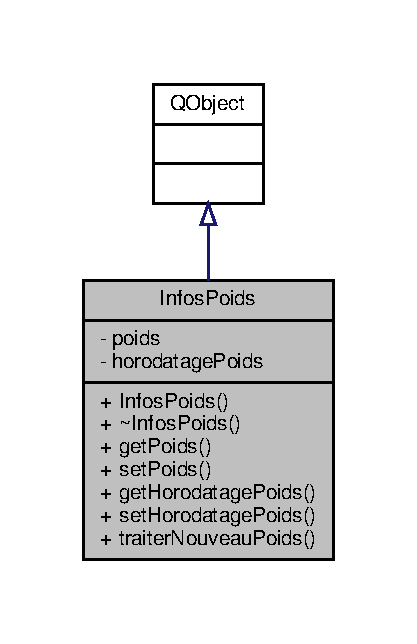
\includegraphics[width=200pt]{class_infos_poids__coll__graph}
\end{center}
\end{figure}
\subsubsection*{Connecteurs publics}
\begin{DoxyCompactItemize}
\item 
void \hyperlink{class_infos_poids_aa5284d38d33adba31ba033b8af61cc96}{traiter\+Nouveau\+Poids} (Q\+String nouveau\+Poids, Q\+String \hyperlink{class_infos_poids_a6cff463552adfdde9430073a87878494}{horodatage\+Poids})
\end{DoxyCompactItemize}
\subsubsection*{Signaux}
\begin{DoxyCompactItemize}
\item 
void \hyperlink{class_infos_poids_a3c4ca9068911e45d0207de051ef5b402}{poids\+Envoye} (const double \hyperlink{class_infos_poids_ac5faebb99bd0f87f96b442f10349cbd8}{poids}, Q\+String)
\end{DoxyCompactItemize}
\subsubsection*{Fonctions membres publiques}
\begin{DoxyCompactItemize}
\item 
\hyperlink{class_infos_poids_a25a9086e75ce6c7e8391c3908c9324c0}{Infos\+Poids} (\hyperlink{class_q_object}{Q\+Object} $\ast$parent)
\item 
\hyperlink{class_infos_poids_a14038b5639c79ff6558c91aec12013d1}{$\sim$\+Infos\+Poids} ()
\item 
double \hyperlink{class_infos_poids_a902fb0222d3b2fa396987daed57377d2}{get\+Poids} ()
\item 
void \hyperlink{class_infos_poids_a23bb9c5939d0ee5cab0ecf821cdc6779}{set\+Poids} (double \hyperlink{class_infos_poids_ac5faebb99bd0f87f96b442f10349cbd8}{poids})
\item 
Q\+String \hyperlink{class_infos_poids_a9bd9ffa1a5fcd75a8d75bd7330727620}{get\+Horodatage\+Poids} ()
\item 
void \hyperlink{class_infos_poids_add0957f341ade104a4521ead7562dff8}{set\+Horodatage\+Poids} (Q\+String \hyperlink{class_infos_poids_a6cff463552adfdde9430073a87878494}{horodatage\+Poids})
\end{DoxyCompactItemize}
\subsubsection*{Attributs privés}
\begin{DoxyCompactItemize}
\item 
double \hyperlink{class_infos_poids_ac5faebb99bd0f87f96b442f10349cbd8}{poids}
\item 
Q\+String \hyperlink{class_infos_poids_a6cff463552adfdde9430073a87878494}{horodatage\+Poids}
\end{DoxyCompactItemize}


\subsubsection{Description détaillée}
\begin{DoxyAuthor}{Auteur}
Florentin Mellah, Enzo Rossi
\end{DoxyAuthor}
\begin{DoxyVersion}{Version}
1.\+1 
\end{DoxyVersion}


\subsubsection{Documentation des constructeurs et destructeur}
\mbox{\Hypertarget{class_infos_poids_a25a9086e75ce6c7e8391c3908c9324c0}\label{class_infos_poids_a25a9086e75ce6c7e8391c3908c9324c0}} 
\index{Infos\+Poids@{Infos\+Poids}!Infos\+Poids@{Infos\+Poids}}
\index{Infos\+Poids@{Infos\+Poids}!Infos\+Poids@{Infos\+Poids}}
\paragraph{\texorpdfstring{Infos\+Poids()}{InfosPoids()}}
{\footnotesize\ttfamily Infos\+Poids\+::\+Infos\+Poids (\begin{DoxyParamCaption}\item[{\hyperlink{class_q_object}{Q\+Object} $\ast$}]{parent }\end{DoxyParamCaption})}


\begin{DoxyCode}
00016                                       : \hyperlink{class_q_object}{QObject}(parent), \hyperlink{class_infos_poids_ac5faebb99bd0f87f96b442f10349cbd8}{poids}(0) , 
      \hyperlink{class_infos_poids_a6cff463552adfdde9430073a87878494}{horodatagePoids}(\textcolor{stringliteral}{""})
00017 \{
00018 \}
\end{DoxyCode}
\mbox{\Hypertarget{class_infos_poids_a14038b5639c79ff6558c91aec12013d1}\label{class_infos_poids_a14038b5639c79ff6558c91aec12013d1}} 
\index{Infos\+Poids@{Infos\+Poids}!````~Infos\+Poids@{$\sim$\+Infos\+Poids}}
\index{````~Infos\+Poids@{$\sim$\+Infos\+Poids}!Infos\+Poids@{Infos\+Poids}}
\paragraph{\texorpdfstring{$\sim$\+Infos\+Poids()}{~InfosPoids()}}
{\footnotesize\ttfamily Infos\+Poids\+::$\sim$\+Infos\+Poids (\begin{DoxyParamCaption}{ }\end{DoxyParamCaption})}


\begin{DoxyCode}
00021 \{
00022 \}
\end{DoxyCode}


\subsubsection{Documentation des fonctions membres}
\mbox{\Hypertarget{class_infos_poids_a9bd9ffa1a5fcd75a8d75bd7330727620}\label{class_infos_poids_a9bd9ffa1a5fcd75a8d75bd7330727620}} 
\index{Infos\+Poids@{Infos\+Poids}!get\+Horodatage\+Poids@{get\+Horodatage\+Poids}}
\index{get\+Horodatage\+Poids@{get\+Horodatage\+Poids}!Infos\+Poids@{Infos\+Poids}}
\paragraph{\texorpdfstring{get\+Horodatage\+Poids()}{getHorodatagePoids()}}
{\footnotesize\ttfamily Q\+String Infos\+Poids\+::get\+Horodatage\+Poids (\begin{DoxyParamCaption}{ }\end{DoxyParamCaption})}



Références \hyperlink{class_infos_poids_a6cff463552adfdde9430073a87878494}{horodatage\+Poids}.



Référencé par \hyperlink{class_ruche_a923f42fc4878a01f6102966a748e8f37}{Ruche\+::inserer\+Donnees\+Port\+Poids()}.


\begin{DoxyCode}
00043 \{
00044     \textcolor{keywordflow}{return} \hyperlink{class_infos_poids_a6cff463552adfdde9430073a87878494}{horodatagePoids};
00045 \}
\end{DoxyCode}
\mbox{\Hypertarget{class_infos_poids_a902fb0222d3b2fa396987daed57377d2}\label{class_infos_poids_a902fb0222d3b2fa396987daed57377d2}} 
\index{Infos\+Poids@{Infos\+Poids}!get\+Poids@{get\+Poids}}
\index{get\+Poids@{get\+Poids}!Infos\+Poids@{Infos\+Poids}}
\paragraph{\texorpdfstring{get\+Poids()}{getPoids()}}
{\footnotesize\ttfamily double Infos\+Poids\+::get\+Poids (\begin{DoxyParamCaption}{ }\end{DoxyParamCaption})}



Références \hyperlink{class_infos_poids_ac5faebb99bd0f87f96b442f10349cbd8}{poids}.



Référencé par \hyperlink{class_alertes_ac4b8925cc6c262cf7254b1576ba07d33}{Alertes\+::alertes\+Poids()}.


\begin{DoxyCode}
00025 \{
00026     \textcolor{keywordflow}{return} \hyperlink{class_infos_poids_ac5faebb99bd0f87f96b442f10349cbd8}{poids};
00027 \}
\end{DoxyCode}
\mbox{\Hypertarget{class_infos_poids_a3c4ca9068911e45d0207de051ef5b402}\label{class_infos_poids_a3c4ca9068911e45d0207de051ef5b402}} 
\index{Infos\+Poids@{Infos\+Poids}!poids\+Envoye@{poids\+Envoye}}
\index{poids\+Envoye@{poids\+Envoye}!Infos\+Poids@{Infos\+Poids}}
\paragraph{\texorpdfstring{poids\+Envoye}{poidsEnvoye}}
{\footnotesize\ttfamily void Infos\+Poids\+::poids\+Envoye (\begin{DoxyParamCaption}\item[{const double}]{poids,  }\item[{Q\+String}]{ }\end{DoxyParamCaption})\hspace{0.3cm}{\ttfamily [signal]}}



Référencé par \hyperlink{class_infos_poids_aa5284d38d33adba31ba033b8af61cc96}{traiter\+Nouveau\+Poids()}.

\mbox{\Hypertarget{class_infos_poids_add0957f341ade104a4521ead7562dff8}\label{class_infos_poids_add0957f341ade104a4521ead7562dff8}} 
\index{Infos\+Poids@{Infos\+Poids}!set\+Horodatage\+Poids@{set\+Horodatage\+Poids}}
\index{set\+Horodatage\+Poids@{set\+Horodatage\+Poids}!Infos\+Poids@{Infos\+Poids}}
\paragraph{\texorpdfstring{set\+Horodatage\+Poids()}{setHorodatagePoids()}}
{\footnotesize\ttfamily void Infos\+Poids\+::set\+Horodatage\+Poids (\begin{DoxyParamCaption}\item[{Q\+String}]{horodatage\+Poids }\end{DoxyParamCaption})}



Références \hyperlink{class_infos_poids_a6cff463552adfdde9430073a87878494}{horodatage\+Poids}.


\begin{DoxyCode}
00047 \{
00048     this->\hyperlink{class_infos_poids_a6cff463552adfdde9430073a87878494}{horodatagePoids} = \hyperlink{class_infos_poids_a6cff463552adfdde9430073a87878494}{horodatagePoids};
00049 \}
\end{DoxyCode}
\mbox{\Hypertarget{class_infos_poids_a23bb9c5939d0ee5cab0ecf821cdc6779}\label{class_infos_poids_a23bb9c5939d0ee5cab0ecf821cdc6779}} 
\index{Infos\+Poids@{Infos\+Poids}!set\+Poids@{set\+Poids}}
\index{set\+Poids@{set\+Poids}!Infos\+Poids@{Infos\+Poids}}
\paragraph{\texorpdfstring{set\+Poids()}{setPoids()}}
{\footnotesize\ttfamily void Infos\+Poids\+::set\+Poids (\begin{DoxyParamCaption}\item[{double}]{poids }\end{DoxyParamCaption})}



Références \hyperlink{class_infos_poids_ac5faebb99bd0f87f96b442f10349cbd8}{poids}.


\begin{DoxyCode}
00030 \{
00031     this->\hyperlink{class_infos_poids_ac5faebb99bd0f87f96b442f10349cbd8}{poids} = \hyperlink{class_infos_poids_ac5faebb99bd0f87f96b442f10349cbd8}{poids};
00032 \}
\end{DoxyCode}
\mbox{\Hypertarget{class_infos_poids_aa5284d38d33adba31ba033b8af61cc96}\label{class_infos_poids_aa5284d38d33adba31ba033b8af61cc96}} 
\index{Infos\+Poids@{Infos\+Poids}!traiter\+Nouveau\+Poids@{traiter\+Nouveau\+Poids}}
\index{traiter\+Nouveau\+Poids@{traiter\+Nouveau\+Poids}!Infos\+Poids@{Infos\+Poids}}
\paragraph{\texorpdfstring{traiter\+Nouveau\+Poids}{traiterNouveauPoids}}
{\footnotesize\ttfamily void Infos\+Poids\+::traiter\+Nouveau\+Poids (\begin{DoxyParamCaption}\item[{Q\+String}]{nouveau\+Poids,  }\item[{Q\+String}]{horodatage\+Poids }\end{DoxyParamCaption})\hspace{0.3cm}{\ttfamily [slot]}}



Références \hyperlink{class_infos_poids_a6cff463552adfdde9430073a87878494}{horodatage\+Poids}, \hyperlink{class_infos_poids_ac5faebb99bd0f87f96b442f10349cbd8}{poids}, et \hyperlink{class_infos_poids_a3c4ca9068911e45d0207de051ef5b402}{poids\+Envoye()}.


\begin{DoxyCode}
00035 \{
00036     this->\hyperlink{class_infos_poids_a6cff463552adfdde9430073a87878494}{horodatagePoids} = \hyperlink{class_infos_poids_a6cff463552adfdde9430073a87878494}{horodatagePoids};
00037     \hyperlink{class_infos_poids_ac5faebb99bd0f87f96b442f10349cbd8}{poids} = nouveauPoids.toDouble() / 1000;
00038     emit \hyperlink{class_infos_poids_a3c4ca9068911e45d0207de051ef5b402}{poidsEnvoye}(\hyperlink{class_infos_poids_ac5faebb99bd0f87f96b442f10349cbd8}{poids},\hyperlink{class_infos_poids_a6cff463552adfdde9430073a87878494}{horodatagePoids});
00039     qDebug() << Q\_FUNC\_INFO << \textcolor{stringliteral}{"poids = "} << \hyperlink{class_infos_poids_ac5faebb99bd0f87f96b442f10349cbd8}{poids};
00040 \}
\end{DoxyCode}


\subsubsection{Documentation des données membres}
\mbox{\Hypertarget{class_infos_poids_a6cff463552adfdde9430073a87878494}\label{class_infos_poids_a6cff463552adfdde9430073a87878494}} 
\index{Infos\+Poids@{Infos\+Poids}!horodatage\+Poids@{horodatage\+Poids}}
\index{horodatage\+Poids@{horodatage\+Poids}!Infos\+Poids@{Infos\+Poids}}
\paragraph{\texorpdfstring{horodatage\+Poids}{horodatagePoids}}
{\footnotesize\ttfamily Q\+String Infos\+Poids\+::horodatage\+Poids\hspace{0.3cm}{\ttfamily [private]}}



Référencé par \hyperlink{class_infos_poids_a9bd9ffa1a5fcd75a8d75bd7330727620}{get\+Horodatage\+Poids()}, \hyperlink{class_infos_poids_add0957f341ade104a4521ead7562dff8}{set\+Horodatage\+Poids()}, et \hyperlink{class_infos_poids_aa5284d38d33adba31ba033b8af61cc96}{traiter\+Nouveau\+Poids()}.

\mbox{\Hypertarget{class_infos_poids_ac5faebb99bd0f87f96b442f10349cbd8}\label{class_infos_poids_ac5faebb99bd0f87f96b442f10349cbd8}} 
\index{Infos\+Poids@{Infos\+Poids}!poids@{poids}}
\index{poids@{poids}!Infos\+Poids@{Infos\+Poids}}
\paragraph{\texorpdfstring{poids}{poids}}
{\footnotesize\ttfamily double Infos\+Poids\+::poids\hspace{0.3cm}{\ttfamily [private]}}



Référencé par \hyperlink{class_infos_poids_a902fb0222d3b2fa396987daed57377d2}{get\+Poids()}, \hyperlink{class_infos_poids_a23bb9c5939d0ee5cab0ecf821cdc6779}{set\+Poids()}, et \hyperlink{class_infos_poids_aa5284d38d33adba31ba033b8af61cc96}{traiter\+Nouveau\+Poids()}.



La documentation de cette classe a été générée à partir des fichiers suivants \+:\begin{DoxyCompactItemize}
\item 
\hyperlink{infos_poids_8h}{infos\+Poids.\+h}\item 
\hyperlink{infos_poids_8cpp}{infos\+Poids.\+cpp}\end{DoxyCompactItemize}

\hypertarget{class_infos_pression_atmospherique}{}\subsection{Référence de la classe Infos\+Pression\+Atmospherique}
\label{class_infos_pression_atmospherique}\index{Infos\+Pression\+Atmospherique@{Infos\+Pression\+Atmospherique}}


La classe \hyperlink{class_infos_pression_atmospherique}{Infos\+Pression\+Atmospherique}.  




{\ttfamily \#include $<$infos\+Pression\+Atmospherique.\+h$>$}



Graphe de collaboration de Infos\+Pression\+Atmospherique\+:\nopagebreak
\begin{figure}[H]
\begin{center}
\leavevmode
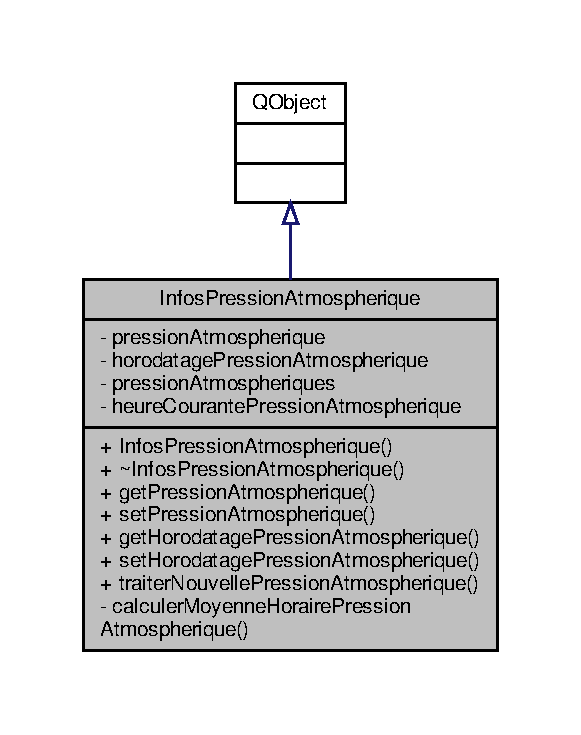
\includegraphics[width=279pt]{class_infos_pression_atmospherique__coll__graph}
\end{center}
\end{figure}
\subsubsection*{Connecteurs publics}
\begin{DoxyCompactItemize}
\item 
void \hyperlink{class_infos_pression_atmospherique_ab280f47f2a1376222a45fde8638489d2}{traiter\+Nouvelle\+Pression\+Atmospherique} (Q\+String pression\+Atmospherique\+String, Q\+String \hyperlink{class_infos_pression_atmospherique_aba207458a51a9290e4f2e0795983a44e}{horodatage\+Pression\+Atmospherique})
\begin{DoxyCompactList}\small\item\em slot qui traite la pression atmospherique \end{DoxyCompactList}\end{DoxyCompactItemize}
\subsubsection*{Signaux}
\begin{DoxyCompactItemize}
\item 
void \hyperlink{class_infos_pression_atmospherique_ad5342b25c87fd5e41a89ad74b5f69c86}{pression\+Atmospherique\+Envoye} (double \hyperlink{class_infos_pression_atmospherique_a69f31dc0d0ef59f8ced23e4663ee1ab8}{pression\+Atmospherique}, Q\+String horodatage)
\item 
void \hyperlink{class_infos_pression_atmospherique_af759842c05a1e59b56d433e823bee341}{traitement\+Pression\+Atmospherique\+Envoye} (const double pression\+Atmospherique\+Moyenne, const double pression\+Atmospherique\+Minimum, const double pression\+Atmospherique\+Maximum, int heure)
\end{DoxyCompactItemize}
\subsubsection*{Fonctions membres publiques}
\begin{DoxyCompactItemize}
\item 
\hyperlink{class_infos_pression_atmospherique_aade2e8de08264974305962bea890bf68}{Infos\+Pression\+Atmospherique} (\hyperlink{class_q_object}{Q\+Object} $\ast$parent)
\item 
\hyperlink{class_infos_pression_atmospherique_a3f4d667523391ceb3c2342c70a3ee41f}{$\sim$\+Infos\+Pression\+Atmospherique} ()
\begin{DoxyCompactList}\small\item\em destructeur de la classe \hyperlink{class_infos_pression_atmospherique}{Infos\+Pression\+Atmospherique} \end{DoxyCompactList}\item 
double \hyperlink{class_infos_pression_atmospherique_ace9906ecdd245d4d443554fcc77c76a5}{get\+Pression\+Atmospherique} ()
\begin{DoxyCompactList}\small\item\em getter de l\textquotesingle{}attribut pression\+Atmospherique \end{DoxyCompactList}\item 
void \hyperlink{class_infos_pression_atmospherique_ab598771e222fbca604ac6dba5d2aacb9}{set\+Pression\+Atmospherique} (double \hyperlink{class_infos_pression_atmospherique_a69f31dc0d0ef59f8ced23e4663ee1ab8}{pression\+Atmospherique})
\begin{DoxyCompactList}\small\item\em setter de l\textquotesingle{}attribut pression\+Atmospherique \end{DoxyCompactList}\item 
Q\+String \hyperlink{class_infos_pression_atmospherique_a6836dfc16f1be4287354ea26a080b436}{get\+Horodatage\+Pression\+Atmospherique} () const
\begin{DoxyCompactList}\small\item\em getter de l\textquotesingle{}attribut horodatage\+Pression\+Atmospherique \end{DoxyCompactList}\item 
void \hyperlink{class_infos_pression_atmospherique_a5d8ba94db66bb7bcdf5a70dd6f21de23}{set\+Horodatage\+Pression\+Atmospherique} (const Q\+String \hyperlink{class_infos_pression_atmospherique_aba207458a51a9290e4f2e0795983a44e}{horodatage\+Pression\+Atmospherique})
\begin{DoxyCompactList}\small\item\em setter de l\textquotesingle{}attribut horodatage\+Pression\+Atmospherique \end{DoxyCompactList}\end{DoxyCompactItemize}
\subsubsection*{Fonctions membres privées}
\begin{DoxyCompactItemize}
\item 
void \hyperlink{class_infos_pression_atmospherique_a287f1f24726218868c8531365c1a22ec}{calculer\+Moyenne\+Horaire\+Pression\+Atmospherique} ()
\end{DoxyCompactItemize}
\subsubsection*{Attributs privés}
\begin{DoxyCompactItemize}
\item 
double \hyperlink{class_infos_pression_atmospherique_a69f31dc0d0ef59f8ced23e4663ee1ab8}{pression\+Atmospherique}
\begin{DoxyCompactList}\small\item\em la pression atmospherique (unité ?) \end{DoxyCompactList}\item 
Q\+String \hyperlink{class_infos_pression_atmospherique_aba207458a51a9290e4f2e0795983a44e}{horodatage\+Pression\+Atmospherique}
\begin{DoxyCompactList}\small\item\em horodatage de la pression atmospherique \end{DoxyCompactList}\item 
Q\+Vector$<$ double $>$ \hyperlink{class_infos_pression_atmospherique_a38218b11dc9fb22aca7525f93155a26c}{pression\+Atmospheriques}
\item 
int \hyperlink{class_infos_pression_atmospherique_ab3fa5c89841cf03f371ef7848b8bc958}{heure\+Courante\+Pression\+Atmospherique}
\end{DoxyCompactItemize}


\subsubsection{Description détaillée}
\begin{DoxyAuthor}{Auteur}
Florentin Mellah, Enzo Rossi
\end{DoxyAuthor}
\begin{DoxyVersion}{Version}
1.\+1 
\end{DoxyVersion}


\subsubsection{Documentation des constructeurs et destructeur}
\mbox{\Hypertarget{class_infos_pression_atmospherique_aade2e8de08264974305962bea890bf68}\label{class_infos_pression_atmospherique_aade2e8de08264974305962bea890bf68}} 
\index{Infos\+Pression\+Atmospherique@{Infos\+Pression\+Atmospherique}!Infos\+Pression\+Atmospherique@{Infos\+Pression\+Atmospherique}}
\index{Infos\+Pression\+Atmospherique@{Infos\+Pression\+Atmospherique}!Infos\+Pression\+Atmospherique@{Infos\+Pression\+Atmospherique}}
\paragraph{\texorpdfstring{Infos\+Pression\+Atmospherique()}{InfosPressionAtmospherique()}}
{\footnotesize\ttfamily Infos\+Pression\+Atmospherique\+::\+Infos\+Pression\+Atmospherique (\begin{DoxyParamCaption}\item[{\hyperlink{class_q_object}{Q\+Object} $\ast$}]{parent }\end{DoxyParamCaption})}


\begin{DoxyCode}
00026                                                                      : \hyperlink{class_q_object}{QObject}(parent), 
      \hyperlink{class_infos_pression_atmospherique_a69f31dc0d0ef59f8ced23e4663ee1ab8}{pressionAtmospherique}(0), \hyperlink{class_infos_pression_atmospherique_aba207458a51a9290e4f2e0795983a44e}{horodatagePressionAtmospherique}
      (\textcolor{stringliteral}{""}),\hyperlink{class_infos_pression_atmospherique_ab3fa5c89841cf03f371ef7848b8bc958}{heureCourantePressionAtmospherique}(-1)
00027 \{
00028 \}
\end{DoxyCode}
\mbox{\Hypertarget{class_infos_pression_atmospherique_a3f4d667523391ceb3c2342c70a3ee41f}\label{class_infos_pression_atmospherique_a3f4d667523391ceb3c2342c70a3ee41f}} 
\index{Infos\+Pression\+Atmospherique@{Infos\+Pression\+Atmospherique}!````~Infos\+Pression\+Atmospherique@{$\sim$\+Infos\+Pression\+Atmospherique}}
\index{````~Infos\+Pression\+Atmospherique@{$\sim$\+Infos\+Pression\+Atmospherique}!Infos\+Pression\+Atmospherique@{Infos\+Pression\+Atmospherique}}
\paragraph{\texorpdfstring{$\sim$\+Infos\+Pression\+Atmospherique()}{~InfosPressionAtmospherique()}}
{\footnotesize\ttfamily Infos\+Pression\+Atmospherique\+::$\sim$\+Infos\+Pression\+Atmospherique (\begin{DoxyParamCaption}{ }\end{DoxyParamCaption})}


\begin{DoxyCode}
00034 \{
00035 \}
\end{DoxyCode}


\subsubsection{Documentation des fonctions membres}
\mbox{\Hypertarget{class_infos_pression_atmospherique_a287f1f24726218868c8531365c1a22ec}\label{class_infos_pression_atmospherique_a287f1f24726218868c8531365c1a22ec}} 
\index{Infos\+Pression\+Atmospherique@{Infos\+Pression\+Atmospherique}!calculer\+Moyenne\+Horaire\+Pression\+Atmospherique@{calculer\+Moyenne\+Horaire\+Pression\+Atmospherique}}
\index{calculer\+Moyenne\+Horaire\+Pression\+Atmospherique@{calculer\+Moyenne\+Horaire\+Pression\+Atmospherique}!Infos\+Pression\+Atmospherique@{Infos\+Pression\+Atmospherique}}
\paragraph{\texorpdfstring{calculer\+Moyenne\+Horaire\+Pression\+Atmospherique()}{calculerMoyenneHorairePressionAtmospherique()}}
{\footnotesize\ttfamily void Infos\+Pression\+Atmospherique\+::calculer\+Moyenne\+Horaire\+Pression\+Atmospherique (\begin{DoxyParamCaption}{ }\end{DoxyParamCaption})\hspace{0.3cm}{\ttfamily [private]}}



Références \hyperlink{class_infos_pression_atmospherique_ab3fa5c89841cf03f371ef7848b8bc958}{heure\+Courante\+Pression\+Atmospherique}, \hyperlink{class_infos_pression_atmospherique_a38218b11dc9fb22aca7525f93155a26c}{pression\+Atmospheriques}, et \hyperlink{class_infos_pression_atmospherique_af759842c05a1e59b56d433e823bee341}{traitement\+Pression\+Atmospherique\+Envoye()}.



Référencé par \hyperlink{class_infos_pression_atmospherique_ab280f47f2a1376222a45fde8638489d2}{traiter\+Nouvelle\+Pression\+Atmospherique()}.


\begin{DoxyCode}
00105 \{
00106     \textcolor{keywordtype}{double} sommePressionAtmospherique= 0;
00107     \textcolor{keywordtype}{double} pressionAtmospheriqueMoyenne = 0;
00108     \textcolor{keywordtype}{double} pressionAtmospheriqueMinimum = 1200;
00109     \textcolor{keywordtype}{double} pressionAtmospheriqueMaximum = -999;
00110 
00111     \textcolor{comment}{// au moins 2 mesures}
00112     \textcolor{keywordflow}{if}(\hyperlink{class_infos_pression_atmospherique_a38218b11dc9fb22aca7525f93155a26c}{pressionAtmospheriques}.size() >= 2)
00113     \{
00114         pressionAtmospheriqueMinimum = \hyperlink{class_infos_pression_atmospherique_a38218b11dc9fb22aca7525f93155a26c}{pressionAtmospheriques}[0];
00115         pressionAtmospheriqueMaximum = \hyperlink{class_infos_pression_atmospherique_a38218b11dc9fb22aca7525f93155a26c}{pressionAtmospheriques}[0];
00116         \textcolor{keywordflow}{for} (\textcolor{keywordtype}{int} i = 0; i < \hyperlink{class_infos_pression_atmospherique_a38218b11dc9fb22aca7525f93155a26c}{pressionAtmospheriques}.size(); i++)
00117         \{
00118             sommePressionAtmospherique += \hyperlink{class_infos_pression_atmospherique_a38218b11dc9fb22aca7525f93155a26c}{pressionAtmospheriques}[i];
00119 
00120             \textcolor{keywordflow}{if}(pressionAtmospheriqueMinimum > \hyperlink{class_infos_pression_atmospherique_a38218b11dc9fb22aca7525f93155a26c}{pressionAtmospheriques}[i])
00121             \{
00122                 pressionAtmospheriqueMinimum = \hyperlink{class_infos_pression_atmospherique_a38218b11dc9fb22aca7525f93155a26c}{pressionAtmospheriques}[i];
00123             \}
00124 
00125             \textcolor{keywordflow}{if}(pressionAtmospheriqueMaximum < \hyperlink{class_infos_pression_atmospherique_a38218b11dc9fb22aca7525f93155a26c}{pressionAtmospheriques}[i])
00126             \{
00127                 pressionAtmospheriqueMaximum = \hyperlink{class_infos_pression_atmospherique_a38218b11dc9fb22aca7525f93155a26c}{pressionAtmospheriques}[i];
00128             \}
00129         \}
00130     \}
00131     qDebug() << Q\_FUNC\_INFO << \hyperlink{class_infos_pression_atmospherique_a38218b11dc9fb22aca7525f93155a26c}{pressionAtmospheriques};
00132     pressionAtmospheriqueMoyenne = sommePressionAtmospherique/ double(pressionAtmospheriques.size());
00133     emit \hyperlink{class_infos_pression_atmospherique_af759842c05a1e59b56d433e823bee341}{traitementPressionAtmospheriqueEnvoye}(
      pressionAtmospheriqueMoyenne, pressionAtmospheriqueMinimum ,pressionAtmospheriqueMaximum, 
      \hyperlink{class_infos_pression_atmospherique_ab3fa5c89841cf03f371ef7848b8bc958}{heureCourantePressionAtmospherique});
00134     pressionAtmospheriques.clear();
00135 \}
\end{DoxyCode}
\mbox{\Hypertarget{class_infos_pression_atmospherique_a6836dfc16f1be4287354ea26a080b436}\label{class_infos_pression_atmospherique_a6836dfc16f1be4287354ea26a080b436}} 
\index{Infos\+Pression\+Atmospherique@{Infos\+Pression\+Atmospherique}!get\+Horodatage\+Pression\+Atmospherique@{get\+Horodatage\+Pression\+Atmospherique}}
\index{get\+Horodatage\+Pression\+Atmospherique@{get\+Horodatage\+Pression\+Atmospherique}!Infos\+Pression\+Atmospherique@{Infos\+Pression\+Atmospherique}}
\paragraph{\texorpdfstring{get\+Horodatage\+Pression\+Atmospherique()}{getHorodatagePressionAtmospherique()}}
{\footnotesize\ttfamily Q\+String Infos\+Pression\+Atmospherique\+::get\+Horodatage\+Pression\+Atmospherique (\begin{DoxyParamCaption}{ }\end{DoxyParamCaption}) const}

\begin{DoxyReturn}{Renvoie}
{\itshape Q\+String} horodatage\+Pression\+Atmospherique 
\end{DoxyReturn}


Références \hyperlink{class_infos_pression_atmospherique_aba207458a51a9290e4f2e0795983a44e}{horodatage\+Pression\+Atmospherique}.


\begin{DoxyCode}
00071 \{
00072     \textcolor{keywordflow}{return} \hyperlink{class_infos_pression_atmospherique_aba207458a51a9290e4f2e0795983a44e}{horodatagePressionAtmospherique};
00073 \}
\end{DoxyCode}
\mbox{\Hypertarget{class_infos_pression_atmospherique_ace9906ecdd245d4d443554fcc77c76a5}\label{class_infos_pression_atmospherique_ace9906ecdd245d4d443554fcc77c76a5}} 
\index{Infos\+Pression\+Atmospherique@{Infos\+Pression\+Atmospherique}!get\+Pression\+Atmospherique@{get\+Pression\+Atmospherique}}
\index{get\+Pression\+Atmospherique@{get\+Pression\+Atmospherique}!Infos\+Pression\+Atmospherique@{Infos\+Pression\+Atmospherique}}
\paragraph{\texorpdfstring{get\+Pression\+Atmospherique()}{getPressionAtmospherique()}}
{\footnotesize\ttfamily double Infos\+Pression\+Atmospherique\+::get\+Pression\+Atmospherique (\begin{DoxyParamCaption}{ }\end{DoxyParamCaption})}

\begin{DoxyReturn}{Renvoie}
{\itshape double} pression\+Atmospherique 
\end{DoxyReturn}


Références \hyperlink{class_infos_pression_atmospherique_a69f31dc0d0ef59f8ced23e4663ee1ab8}{pression\+Atmospherique}.



Référencé par \hyperlink{class_alertes_ab8a33e82cdd4d4e0560c9ba6e10ca8d5}{Alertes\+::alertes\+Pression\+Atmospherique()}.


\begin{DoxyCode}
00043 \{
00044     \textcolor{keywordflow}{return} \hyperlink{class_infos_pression_atmospherique_a69f31dc0d0ef59f8ced23e4663ee1ab8}{pressionAtmospherique};
00045 \}
\end{DoxyCode}
\mbox{\Hypertarget{class_infos_pression_atmospherique_ad5342b25c87fd5e41a89ad74b5f69c86}\label{class_infos_pression_atmospherique_ad5342b25c87fd5e41a89ad74b5f69c86}} 
\index{Infos\+Pression\+Atmospherique@{Infos\+Pression\+Atmospherique}!pression\+Atmospherique\+Envoye@{pression\+Atmospherique\+Envoye}}
\index{pression\+Atmospherique\+Envoye@{pression\+Atmospherique\+Envoye}!Infos\+Pression\+Atmospherique@{Infos\+Pression\+Atmospherique}}
\paragraph{\texorpdfstring{pression\+Atmospherique\+Envoye}{pressionAtmospheriqueEnvoye}}
{\footnotesize\ttfamily void Infos\+Pression\+Atmospherique\+::pression\+Atmospherique\+Envoye (\begin{DoxyParamCaption}\item[{double}]{pression\+Atmospherique,  }\item[{Q\+String}]{horodatage }\end{DoxyParamCaption})\hspace{0.3cm}{\ttfamily [signal]}}



Référencé par \hyperlink{class_infos_pression_atmospherique_ab280f47f2a1376222a45fde8638489d2}{traiter\+Nouvelle\+Pression\+Atmospherique()}.

\mbox{\Hypertarget{class_infos_pression_atmospherique_a5d8ba94db66bb7bcdf5a70dd6f21de23}\label{class_infos_pression_atmospherique_a5d8ba94db66bb7bcdf5a70dd6f21de23}} 
\index{Infos\+Pression\+Atmospherique@{Infos\+Pression\+Atmospherique}!set\+Horodatage\+Pression\+Atmospherique@{set\+Horodatage\+Pression\+Atmospherique}}
\index{set\+Horodatage\+Pression\+Atmospherique@{set\+Horodatage\+Pression\+Atmospherique}!Infos\+Pression\+Atmospherique@{Infos\+Pression\+Atmospherique}}
\paragraph{\texorpdfstring{set\+Horodatage\+Pression\+Atmospherique()}{setHorodatagePressionAtmospherique()}}
{\footnotesize\ttfamily void Infos\+Pression\+Atmospherique\+::set\+Horodatage\+Pression\+Atmospherique (\begin{DoxyParamCaption}\item[{const Q\+String}]{horodatage\+Pression\+Atmospherique }\end{DoxyParamCaption})}


\begin{DoxyParams}{Paramètres}
{\em horodatage\+Pression\+Atmospherique} & corespondant a la horodatage\+Pression\+Atmospherique \\
\hline
\end{DoxyParams}


Références \hyperlink{class_infos_pression_atmospherique_aba207458a51a9290e4f2e0795983a44e}{horodatage\+Pression\+Atmospherique}.


\begin{DoxyCode}
00062 \{
00063     this->\hyperlink{class_infos_pression_atmospherique_aba207458a51a9290e4f2e0795983a44e}{horodatagePressionAtmospherique} = 
      \hyperlink{class_infos_pression_atmospherique_aba207458a51a9290e4f2e0795983a44e}{horodatagePressionAtmospherique};
00064 \}
\end{DoxyCode}
\mbox{\Hypertarget{class_infos_pression_atmospherique_ab598771e222fbca604ac6dba5d2aacb9}\label{class_infos_pression_atmospherique_ab598771e222fbca604ac6dba5d2aacb9}} 
\index{Infos\+Pression\+Atmospherique@{Infos\+Pression\+Atmospherique}!set\+Pression\+Atmospherique@{set\+Pression\+Atmospherique}}
\index{set\+Pression\+Atmospherique@{set\+Pression\+Atmospherique}!Infos\+Pression\+Atmospherique@{Infos\+Pression\+Atmospherique}}
\paragraph{\texorpdfstring{set\+Pression\+Atmospherique()}{setPressionAtmospherique()}}
{\footnotesize\ttfamily void Infos\+Pression\+Atmospherique\+::set\+Pression\+Atmospherique (\begin{DoxyParamCaption}\item[{double}]{pression\+Atmospherique }\end{DoxyParamCaption})}


\begin{DoxyParams}{Paramètres}
{\em pression\+Atmospherique} & corespondant a la pression atmospherique \\
\hline
\end{DoxyParams}


Références \hyperlink{class_infos_pression_atmospherique_a69f31dc0d0ef59f8ced23e4663ee1ab8}{pression\+Atmospherique}.


\begin{DoxyCode}
00053 \{
00054     this->\hyperlink{class_infos_pression_atmospherique_a69f31dc0d0ef59f8ced23e4663ee1ab8}{pressionAtmospherique} = \hyperlink{class_infos_pression_atmospherique_a69f31dc0d0ef59f8ced23e4663ee1ab8}{pressionAtmospherique};
00055 \}
\end{DoxyCode}
\mbox{\Hypertarget{class_infos_pression_atmospherique_af759842c05a1e59b56d433e823bee341}\label{class_infos_pression_atmospherique_af759842c05a1e59b56d433e823bee341}} 
\index{Infos\+Pression\+Atmospherique@{Infos\+Pression\+Atmospherique}!traitement\+Pression\+Atmospherique\+Envoye@{traitement\+Pression\+Atmospherique\+Envoye}}
\index{traitement\+Pression\+Atmospherique\+Envoye@{traitement\+Pression\+Atmospherique\+Envoye}!Infos\+Pression\+Atmospherique@{Infos\+Pression\+Atmospherique}}
\paragraph{\texorpdfstring{traitement\+Pression\+Atmospherique\+Envoye}{traitementPressionAtmospheriqueEnvoye}}
{\footnotesize\ttfamily void Infos\+Pression\+Atmospherique\+::traitement\+Pression\+Atmospherique\+Envoye (\begin{DoxyParamCaption}\item[{const double}]{pression\+Atmospherique\+Moyenne,  }\item[{const double}]{pression\+Atmospherique\+Minimum,  }\item[{const double}]{pression\+Atmospherique\+Maximum,  }\item[{int}]{heure }\end{DoxyParamCaption})\hspace{0.3cm}{\ttfamily [signal]}}



Référencé par \hyperlink{class_infos_pression_atmospherique_a287f1f24726218868c8531365c1a22ec}{calculer\+Moyenne\+Horaire\+Pression\+Atmospherique()}.

\mbox{\Hypertarget{class_infos_pression_atmospherique_ab280f47f2a1376222a45fde8638489d2}\label{class_infos_pression_atmospherique_ab280f47f2a1376222a45fde8638489d2}} 
\index{Infos\+Pression\+Atmospherique@{Infos\+Pression\+Atmospherique}!traiter\+Nouvelle\+Pression\+Atmospherique@{traiter\+Nouvelle\+Pression\+Atmospherique}}
\index{traiter\+Nouvelle\+Pression\+Atmospherique@{traiter\+Nouvelle\+Pression\+Atmospherique}!Infos\+Pression\+Atmospherique@{Infos\+Pression\+Atmospherique}}
\paragraph{\texorpdfstring{traiter\+Nouvelle\+Pression\+Atmospherique}{traiterNouvellePressionAtmospherique}}
{\footnotesize\ttfamily void Infos\+Pression\+Atmospherique\+::traiter\+Nouvelle\+Pression\+Atmospherique (\begin{DoxyParamCaption}\item[{Q\+String}]{pression\+Atmospherique\+String,  }\item[{Q\+String}]{horodatage\+Pression\+Atmospherique }\end{DoxyParamCaption})\hspace{0.3cm}{\ttfamily [slot]}}


\begin{DoxyParams}{Paramètres}
{\em pression\+Atmospherique\+String} & qui corespond a la pression atmospherique envoyé par la \hyperlink{class_ruche}{Ruche} \\
\hline
{\em horodatage\+Pression\+Atmospherique} & correspond a l\textquotesingle{}horodatage de la mesure de la pression atmospherique \\
\hline
\end{DoxyParams}


Références \hyperlink{class_infos_pression_atmospherique_a287f1f24726218868c8531365c1a22ec}{calculer\+Moyenne\+Horaire\+Pression\+Atmospherique()}, \hyperlink{class_infos_pression_atmospherique_ab3fa5c89841cf03f371ef7848b8bc958}{heure\+Courante\+Pression\+Atmospherique}, \hyperlink{class_infos_pression_atmospherique_a69f31dc0d0ef59f8ced23e4663ee1ab8}{pression\+Atmospherique}, \hyperlink{class_infos_pression_atmospherique_ad5342b25c87fd5e41a89ad74b5f69c86}{pression\+Atmospherique\+Envoye()}, et \hyperlink{class_infos_pression_atmospherique_a38218b11dc9fb22aca7525f93155a26c}{pression\+Atmospheriques}.


\begin{DoxyCode}
00082 \{
00083     \hyperlink{class_infos_pression_atmospherique_a69f31dc0d0ef59f8ced23e4663ee1ab8}{pressionAtmospherique} = pressionAtmospheriqueString.toDouble();
00084     emit \hyperlink{class_infos_pression_atmospherique_ad5342b25c87fd5e41a89ad74b5f69c86}{pressionAtmospheriqueEnvoye}(
      \hyperlink{class_infos_pression_atmospherique_a69f31dc0d0ef59f8ced23e4663ee1ab8}{pressionAtmospherique},\hyperlink{class_infos_pression_atmospherique_aba207458a51a9290e4f2e0795983a44e}{horodatagePressionAtmospherique});
00085 
00086     QDateTime dateTimeHorodatage = QDateTime::fromString(
      \hyperlink{class_infos_pression_atmospherique_aba207458a51a9290e4f2e0795983a44e}{horodatagePressionAtmospherique}, \textcolor{stringliteral}{"dd/MM/yyyy HH:mm:ss"});
00087     qDebug() << Q\_FUNC\_INFO << \textcolor{stringliteral}{"heureCourantePressionAtmospherique"} << 
      \hyperlink{class_infos_pression_atmospherique_ab3fa5c89841cf03f371ef7848b8bc958}{heureCourantePressionAtmospherique} << dateTimeHorodatage.time().hour();
00088     \textcolor{keywordflow}{if}(\hyperlink{class_infos_pression_atmospherique_ab3fa5c89841cf03f371ef7848b8bc958}{heureCourantePressionAtmospherique} == -1)
00089     \{
00090         \hyperlink{class_infos_pression_atmospherique_ab3fa5c89841cf03f371ef7848b8bc958}{heureCourantePressionAtmospherique} = dateTimeHorodatage.time().
      hour();
00091     \}
00092     \textcolor{keywordflow}{if}(\hyperlink{class_infos_pression_atmospherique_ab3fa5c89841cf03f371ef7848b8bc958}{heureCourantePressionAtmospherique} == dateTimeHorodatage.time().
      hour())
00093     \{
00094         \hyperlink{class_infos_pression_atmospherique_a38218b11dc9fb22aca7525f93155a26c}{pressionAtmospheriques}.append(
      \hyperlink{class_infos_pression_atmospherique_a69f31dc0d0ef59f8ced23e4663ee1ab8}{pressionAtmospherique});
00095     \}
00096     \textcolor{keywordflow}{else} \textcolor{keywordflow}{if}((\hyperlink{class_infos_pression_atmospherique_ab3fa5c89841cf03f371ef7848b8bc958}{heureCourantePressionAtmospherique}+1)%24 == 
      dateTimeHorodatage.time().hour())
00097     \{
00098         \hyperlink{class_infos_pression_atmospherique_a287f1f24726218868c8531365c1a22ec}{calculerMoyenneHorairePressionAtmospherique}();
00099         \hyperlink{class_infos_pression_atmospherique_ab3fa5c89841cf03f371ef7848b8bc958}{heureCourantePressionAtmospherique} = dateTimeHorodatage.time().
      hour();
00100         \hyperlink{class_infos_pression_atmospherique_a38218b11dc9fb22aca7525f93155a26c}{pressionAtmospheriques}.append(
      \hyperlink{class_infos_pression_atmospherique_a69f31dc0d0ef59f8ced23e4663ee1ab8}{pressionAtmospherique});
00101     \}
00102 \}
\end{DoxyCode}


\subsubsection{Documentation des données membres}
\mbox{\Hypertarget{class_infos_pression_atmospherique_ab3fa5c89841cf03f371ef7848b8bc958}\label{class_infos_pression_atmospherique_ab3fa5c89841cf03f371ef7848b8bc958}} 
\index{Infos\+Pression\+Atmospherique@{Infos\+Pression\+Atmospherique}!heure\+Courante\+Pression\+Atmospherique@{heure\+Courante\+Pression\+Atmospherique}}
\index{heure\+Courante\+Pression\+Atmospherique@{heure\+Courante\+Pression\+Atmospherique}!Infos\+Pression\+Atmospherique@{Infos\+Pression\+Atmospherique}}
\paragraph{\texorpdfstring{heure\+Courante\+Pression\+Atmospherique}{heureCourantePressionAtmospherique}}
{\footnotesize\ttfamily int Infos\+Pression\+Atmospherique\+::heure\+Courante\+Pression\+Atmospherique\hspace{0.3cm}{\ttfamily [private]}}



Référencé par \hyperlink{class_infos_pression_atmospherique_a287f1f24726218868c8531365c1a22ec}{calculer\+Moyenne\+Horaire\+Pression\+Atmospherique()}, et \hyperlink{class_infos_pression_atmospherique_ab280f47f2a1376222a45fde8638489d2}{traiter\+Nouvelle\+Pression\+Atmospherique()}.

\mbox{\Hypertarget{class_infos_pression_atmospherique_aba207458a51a9290e4f2e0795983a44e}\label{class_infos_pression_atmospherique_aba207458a51a9290e4f2e0795983a44e}} 
\index{Infos\+Pression\+Atmospherique@{Infos\+Pression\+Atmospherique}!horodatage\+Pression\+Atmospherique@{horodatage\+Pression\+Atmospherique}}
\index{horodatage\+Pression\+Atmospherique@{horodatage\+Pression\+Atmospherique}!Infos\+Pression\+Atmospherique@{Infos\+Pression\+Atmospherique}}
\paragraph{\texorpdfstring{horodatage\+Pression\+Atmospherique}{horodatagePressionAtmospherique}}
{\footnotesize\ttfamily Q\+String Infos\+Pression\+Atmospherique\+::horodatage\+Pression\+Atmospherique\hspace{0.3cm}{\ttfamily [private]}}



Référencé par \hyperlink{class_infos_pression_atmospherique_a6836dfc16f1be4287354ea26a080b436}{get\+Horodatage\+Pression\+Atmospherique()}, et \hyperlink{class_infos_pression_atmospherique_a5d8ba94db66bb7bcdf5a70dd6f21de23}{set\+Horodatage\+Pression\+Atmospherique()}.

\mbox{\Hypertarget{class_infos_pression_atmospherique_a69f31dc0d0ef59f8ced23e4663ee1ab8}\label{class_infos_pression_atmospherique_a69f31dc0d0ef59f8ced23e4663ee1ab8}} 
\index{Infos\+Pression\+Atmospherique@{Infos\+Pression\+Atmospherique}!pression\+Atmospherique@{pression\+Atmospherique}}
\index{pression\+Atmospherique@{pression\+Atmospherique}!Infos\+Pression\+Atmospherique@{Infos\+Pression\+Atmospherique}}
\paragraph{\texorpdfstring{pression\+Atmospherique}{pressionAtmospherique}}
{\footnotesize\ttfamily double Infos\+Pression\+Atmospherique\+::pression\+Atmospherique\hspace{0.3cm}{\ttfamily [private]}}



Référencé par \hyperlink{class_infos_pression_atmospherique_ace9906ecdd245d4d443554fcc77c76a5}{get\+Pression\+Atmospherique()}, \hyperlink{class_infos_pression_atmospherique_ab598771e222fbca604ac6dba5d2aacb9}{set\+Pression\+Atmospherique()}, et \hyperlink{class_infos_pression_atmospherique_ab280f47f2a1376222a45fde8638489d2}{traiter\+Nouvelle\+Pression\+Atmospherique()}.

\mbox{\Hypertarget{class_infos_pression_atmospherique_a38218b11dc9fb22aca7525f93155a26c}\label{class_infos_pression_atmospherique_a38218b11dc9fb22aca7525f93155a26c}} 
\index{Infos\+Pression\+Atmospherique@{Infos\+Pression\+Atmospherique}!pression\+Atmospheriques@{pression\+Atmospheriques}}
\index{pression\+Atmospheriques@{pression\+Atmospheriques}!Infos\+Pression\+Atmospherique@{Infos\+Pression\+Atmospherique}}
\paragraph{\texorpdfstring{pression\+Atmospheriques}{pressionAtmospheriques}}
{\footnotesize\ttfamily Q\+Vector$<$double$>$ Infos\+Pression\+Atmospherique\+::pression\+Atmospheriques\hspace{0.3cm}{\ttfamily [private]}}



Référencé par \hyperlink{class_infos_pression_atmospherique_a287f1f24726218868c8531365c1a22ec}{calculer\+Moyenne\+Horaire\+Pression\+Atmospherique()}, et \hyperlink{class_infos_pression_atmospherique_ab280f47f2a1376222a45fde8638489d2}{traiter\+Nouvelle\+Pression\+Atmospherique()}.



La documentation de cette classe a été générée à partir des fichiers suivants \+:\begin{DoxyCompactItemize}
\item 
\hyperlink{infos_pression_atmospherique_8h}{infos\+Pression\+Atmospherique.\+h}\item 
\hyperlink{infos_pression_atmospherique_8cpp}{infos\+Pression\+Atmospherique.\+cpp}\end{DoxyCompactItemize}

\hypertarget{class_infos_temperature}{}\subsection{Référence de la classe Infos\+Temperature}
\label{class_infos_temperature}\index{Infos\+Temperature@{Infos\+Temperature}}


La classe \hyperlink{class_infos_temperature}{Infos\+Temperature}.  




{\ttfamily \#include $<$infos\+Temperature.\+h$>$}



Graphe de collaboration de Infos\+Temperature\+:\nopagebreak
\begin{figure}[H]
\begin{center}
\leavevmode
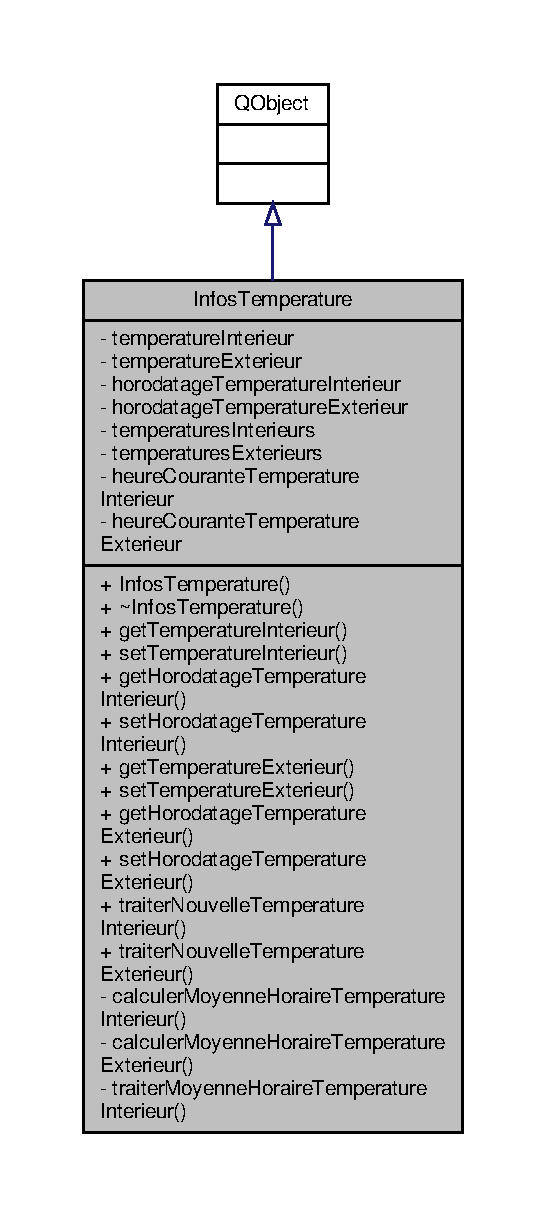
\includegraphics[height=550pt]{class_infos_temperature__coll__graph}
\end{center}
\end{figure}
\subsubsection*{Connecteurs publics}
\begin{DoxyCompactItemize}
\item 
void \hyperlink{class_infos_temperature_a547da18a7c04603d2f30eece061d9634}{traiter\+Nouvelle\+Temperature\+Interieur} (Q\+String \hyperlink{class_infos_temperature_a976ab7ead7ac82b5b8572807d778689e}{temperature\+Interieur}, Q\+String \hyperlink{class_infos_temperature_ad4c62d479b8897102a59025a56d7b4c6}{horodatage\+Temperature\+Interieur})
\item 
void \hyperlink{class_infos_temperature_ab8d95f48c31ca17c8690849562268420}{traiter\+Nouvelle\+Temperature\+Exterieur} (Q\+String temperature\+Exterieur\+String, Q\+String \hyperlink{class_infos_temperature_a5c3cd364746dc1cae5f9faee55c7555e}{horodatage\+Temperature\+Exterieur})
\begin{DoxyCompactList}\small\item\em slot qui traite la temperature exterieur venant de la classe \hyperlink{class_ruche}{Ruche} \end{DoxyCompactList}\end{DoxyCompactItemize}
\subsubsection*{Signaux}
\begin{DoxyCompactItemize}
\item 
void \hyperlink{class_infos_temperature_acaff5cc6bedc53a8bf2c914957d2ab47}{temperature\+Interieur\+Envoye} (const double \hyperlink{class_infos_temperature_a976ab7ead7ac82b5b8572807d778689e}{temperature\+Interieur}, Q\+String horodatage)
\begin{DoxyCompactList}\small\item\em signal vers la classe \hyperlink{class_ruche}{Ruche} \end{DoxyCompactList}\item 
void \hyperlink{class_infos_temperature_a6fbc9ab43714a5ba6649648c15989dee}{temperature\+Exterieur\+Envoye} (const double \hyperlink{class_infos_temperature_af80286a5b0e05d0379f53c0ebbc7d483}{temperature\+Exterieur}, Q\+String horodatage)
\begin{DoxyCompactList}\small\item\em signal vers la classe \hyperlink{class_ruche}{Ruche} \end{DoxyCompactList}\item 
void \hyperlink{class_infos_temperature_a2d7c580a215f918a79aac46a15ff24b9}{traitement\+Temperature\+Interieur\+Envoye} (const double temperature\+Interieur\+Moyenne, const double temperature\+Interieur\+Minimum, const double temperature\+Interieur\+Maximum, int heure)
\item 
void \hyperlink{class_infos_temperature_aaebee9d6151257fa1f182665d0fecf2c}{traitement\+Temperature\+Exterieur\+Envoye} (const double temperature\+Exterieur\+Moyenne, const double temperature\+Exterieur\+Minimum, const double temperature\+Exterieur\+Maximum, int heure)
\end{DoxyCompactItemize}
\subsubsection*{Fonctions membres publiques}
\begin{DoxyCompactItemize}
\item 
\hyperlink{class_infos_temperature_ac628607fe2ff9ca9e2d6bad741ae231a}{Infos\+Temperature} (\hyperlink{class_q_object}{Q\+Object} $\ast$parent)
\begin{DoxyCompactList}\small\item\em Constructeur de la classe \hyperlink{class_infos_pression_atmospherique}{Infos\+Pression\+Atmospherique}. \end{DoxyCompactList}\item 
\hyperlink{class_infos_temperature_a86503a69e48f1919edbb02a434d2b124}{$\sim$\+Infos\+Temperature} ()
\item 
double \hyperlink{class_infos_temperature_aaf4cb4fd8a7c46d14955d3175498f91c}{get\+Temperature\+Interieur} ()
\begin{DoxyCompactList}\small\item\em getter de l\textquotesingle{}attribut temperature\+Interieur \end{DoxyCompactList}\item 
void \hyperlink{class_infos_temperature_ac11ec6b1860f43dc989a02a7967497e7}{set\+Temperature\+Interieur} (double \hyperlink{class_infos_temperature_a976ab7ead7ac82b5b8572807d778689e}{temperature\+Interieur})
\item 
Q\+String \hyperlink{class_infos_temperature_aca40f109786cf22d78402f8b7f3fe408}{get\+Horodatage\+Temperature\+Interieur} ()
\begin{DoxyCompactList}\small\item\em getter de l\textquotesingle{}attribut horodatagetemperature\+Interieur \end{DoxyCompactList}\item 
void \hyperlink{class_infos_temperature_a4d846391dfd204515e68c3f005b7be3c}{set\+Horodatage\+Temperature\+Interieur} (const Q\+String \hyperlink{class_infos_temperature_ad4c62d479b8897102a59025a56d7b4c6}{horodatage\+Temperature\+Interieur})
\item 
double \hyperlink{class_infos_temperature_aebb00308151b8b6319732b62bd7b4b55}{get\+Temperature\+Exterieur} ()
\begin{DoxyCompactList}\small\item\em getter de l\textquotesingle{}attribut temperature\+Exterieur \end{DoxyCompactList}\item 
void \hyperlink{class_infos_temperature_a40f22fbc27ed768e8269cdbf3df708c6}{set\+Temperature\+Exterieur} (double \hyperlink{class_infos_temperature_af80286a5b0e05d0379f53c0ebbc7d483}{temperature\+Exterieur})
\begin{DoxyCompactList}\small\item\em setter de l\textquotesingle{}attribut temperature\+Exterieur \end{DoxyCompactList}\item 
Q\+String \hyperlink{class_infos_temperature_a76b07dc0790718e134e306fe760e6cbf}{get\+Horodatage\+Temperature\+Exterieur} ()
\item 
void \hyperlink{class_infos_temperature_a85118414b65a715d07a92df3059c6fea}{set\+Horodatage\+Temperature\+Exterieur} (const Q\+String \hyperlink{class_infos_temperature_a5c3cd364746dc1cae5f9faee55c7555e}{horodatage\+Temperature\+Exterieur})
\begin{DoxyCompactList}\small\item\em setter de l\textquotesingle{}attribut horodatage\+Temperature\+Exterieur \end{DoxyCompactList}\end{DoxyCompactItemize}
\subsubsection*{Fonctions membres privées}
\begin{DoxyCompactItemize}
\item 
void \hyperlink{class_infos_temperature_a8cb8b9bef07506019ea6c9d91809af87}{calculer\+Moyenne\+Horaire\+Temperature\+Interieur} ()
\begin{DoxyCompactList}\small\item\em methode permettant de calculer la moyenne des temperatures interieurs sur une heure \end{DoxyCompactList}\item 
void \hyperlink{class_infos_temperature_a437325028225d765780b884614c47077}{calculer\+Moyenne\+Horaire\+Temperature\+Exterieur} ()
\begin{DoxyCompactList}\small\item\em methode permettant de calculer la moyenne des temperatures exterieurs sur une heure \end{DoxyCompactList}\item 
void \hyperlink{class_infos_temperature_a0311c8ce5730388f3baef752920d5abf}{traiter\+Moyenne\+Horaire\+Temperature\+Interieur} (Q\+String \hyperlink{class_infos_temperature_ad4c62d479b8897102a59025a56d7b4c6}{horodatage\+Temperature\+Interieur})
\begin{DoxyCompactList}\small\item\em slot qui traite la temperature interieur venant de la classe \hyperlink{class_ruche}{Ruche} \end{DoxyCompactList}\end{DoxyCompactItemize}
\subsubsection*{Attributs privés}
\begin{DoxyCompactItemize}
\item 
double \hyperlink{class_infos_temperature_a976ab7ead7ac82b5b8572807d778689e}{temperature\+Interieur}
\begin{DoxyCompactList}\small\item\em temperature interieur en degrée Celsius \end{DoxyCompactList}\item 
double \hyperlink{class_infos_temperature_af80286a5b0e05d0379f53c0ebbc7d483}{temperature\+Exterieur}
\begin{DoxyCompactList}\small\item\em temperature exterieuren degrée Celsius \end{DoxyCompactList}\item 
Q\+String \hyperlink{class_infos_temperature_ad4c62d479b8897102a59025a56d7b4c6}{horodatage\+Temperature\+Interieur}
\begin{DoxyCompactList}\small\item\em horodatage de la temperature interieur \end{DoxyCompactList}\item 
Q\+String \hyperlink{class_infos_temperature_a5c3cd364746dc1cae5f9faee55c7555e}{horodatage\+Temperature\+Exterieur}
\begin{DoxyCompactList}\small\item\em horodatage de la temperature exterieur \end{DoxyCompactList}\item 
Q\+Vector$<$ double $>$ \hyperlink{class_infos_temperature_a39a976c10811a7589e4aba42586813c5}{temperatures\+Interieurs}
\item 
Q\+Vector$<$ double $>$ \hyperlink{class_infos_temperature_a32b2a36e737ab4bf61fc8274990c2943}{temperatures\+Exterieurs}
\item 
int \hyperlink{class_infos_temperature_a708b70383d309fa0ba355dcc3921cc23}{heure\+Courante\+Temperature\+Interieur}
\item 
int \hyperlink{class_infos_temperature_a44edcf244175896e28798f252900f774}{heure\+Courante\+Temperature\+Exterieur}
\end{DoxyCompactItemize}


\subsubsection{Description détaillée}
\begin{DoxyAuthor}{Auteur}
Florentin Mellah, Enzo Rossi
\end{DoxyAuthor}
\begin{DoxyVersion}{Version}
1.\+1 
\end{DoxyVersion}


\subsubsection{Documentation des constructeurs et destructeur}
\mbox{\Hypertarget{class_infos_temperature_ac628607fe2ff9ca9e2d6bad741ae231a}\label{class_infos_temperature_ac628607fe2ff9ca9e2d6bad741ae231a}} 
\index{Infos\+Temperature@{Infos\+Temperature}!Infos\+Temperature@{Infos\+Temperature}}
\index{Infos\+Temperature@{Infos\+Temperature}!Infos\+Temperature@{Infos\+Temperature}}
\paragraph{\texorpdfstring{Infos\+Temperature()}{InfosTemperature()}}
{\footnotesize\ttfamily Infos\+Temperature\+::\+Infos\+Temperature (\begin{DoxyParamCaption}\item[{\hyperlink{class_q_object}{Q\+Object} $\ast$}]{parent }\end{DoxyParamCaption})}

Constructeur de la classe \hyperlink{class_infos_temperature}{Infos\+Temperature}.

Définition des attributs pression\+Atmospherique à 0 et l\textquotesingle{}attribut horodatage\+Pression\+Atmospherique à \char`\"{}\char`\"{}

Définition des attributs temperature\+Interieur, temperature\+Exterieur à 0 et les attributs temperature\+Exterieur horodatage\+Temperature\+Exterieur à \char`\"{}\char`\"{}


\begin{DoxyParams}{Paramètres}
{\em parent} & \hyperlink{class_q_object}{Q\+Object} Adresse de l\textquotesingle{}objet Qt parent \\
\hline
\end{DoxyParams}

\begin{DoxyCode}
00026                                                  :\hyperlink{class_q_object}{QObject}(parent),
      \hyperlink{class_infos_temperature_a976ab7ead7ac82b5b8572807d778689e}{temperatureInterieur}(0),\hyperlink{class_infos_temperature_af80286a5b0e05d0379f53c0ebbc7d483}{temperatureExterieur}(0),
      \hyperlink{class_infos_temperature_ad4c62d479b8897102a59025a56d7b4c6}{horodatageTemperatureInterieur}(\textcolor{stringliteral}{""}),
      \hyperlink{class_infos_temperature_a5c3cd364746dc1cae5f9faee55c7555e}{horodatageTemperatureExterieur}(\textcolor{stringliteral}{""}),
      \hyperlink{class_infos_temperature_a708b70383d309fa0ba355dcc3921cc23}{heureCouranteTemperatureInterieur}(-1),
      \hyperlink{class_infos_temperature_a44edcf244175896e28798f252900f774}{heureCouranteTemperatureExterieur}(-1)
00027 \{
00028 \}
\end{DoxyCode}
\mbox{\Hypertarget{class_infos_temperature_a86503a69e48f1919edbb02a434d2b124}\label{class_infos_temperature_a86503a69e48f1919edbb02a434d2b124}} 
\index{Infos\+Temperature@{Infos\+Temperature}!````~Infos\+Temperature@{$\sim$\+Infos\+Temperature}}
\index{````~Infos\+Temperature@{$\sim$\+Infos\+Temperature}!Infos\+Temperature@{Infos\+Temperature}}
\paragraph{\texorpdfstring{$\sim$\+Infos\+Temperature()}{~InfosTemperature()}}
{\footnotesize\ttfamily Infos\+Temperature\+::$\sim$\+Infos\+Temperature (\begin{DoxyParamCaption}{ }\end{DoxyParamCaption})}


\begin{DoxyCode}
00031 \{
00032 \}
\end{DoxyCode}


\subsubsection{Documentation des fonctions membres}
\mbox{\Hypertarget{class_infos_temperature_a437325028225d765780b884614c47077}\label{class_infos_temperature_a437325028225d765780b884614c47077}} 
\index{Infos\+Temperature@{Infos\+Temperature}!calculer\+Moyenne\+Horaire\+Temperature\+Exterieur@{calculer\+Moyenne\+Horaire\+Temperature\+Exterieur}}
\index{calculer\+Moyenne\+Horaire\+Temperature\+Exterieur@{calculer\+Moyenne\+Horaire\+Temperature\+Exterieur}!Infos\+Temperature@{Infos\+Temperature}}
\paragraph{\texorpdfstring{calculer\+Moyenne\+Horaire\+Temperature\+Exterieur()}{calculerMoyenneHoraireTemperatureExterieur()}}
{\footnotesize\ttfamily void Infos\+Temperature\+::calculer\+Moyenne\+Horaire\+Temperature\+Exterieur (\begin{DoxyParamCaption}{ }\end{DoxyParamCaption})\hspace{0.3cm}{\ttfamily [private]}}



Références \hyperlink{class_infos_temperature_a44edcf244175896e28798f252900f774}{heure\+Courante\+Temperature\+Exterieur}, \hyperlink{class_infos_temperature_a32b2a36e737ab4bf61fc8274990c2943}{temperatures\+Exterieurs}, et \hyperlink{class_infos_temperature_aaebee9d6151257fa1f182665d0fecf2c}{traitement\+Temperature\+Exterieur\+Envoye()}.



Référencé par \hyperlink{class_infos_temperature_ab8d95f48c31ca17c8690849562268420}{traiter\+Nouvelle\+Temperature\+Exterieur()}.


\begin{DoxyCode}
00232 \{
00233     \textcolor{keywordtype}{double} sommeTemperatureExterieur = 0;
00234     \textcolor{keywordtype}{double} temperatureExterieurMoyenne = 0;
00235     \textcolor{keywordtype}{double} temperatureExterieurMinimum = 999;
00236     \textcolor{keywordtype}{double} temperatureExterieurMaximum = -999;
00237 
00238     \textcolor{comment}{// au moins 2 mesures}
00239     \textcolor{keywordflow}{if}(\hyperlink{class_infos_temperature_a32b2a36e737ab4bf61fc8274990c2943}{temperaturesExterieurs}.size() >= 2)
00240     \{
00241         temperatureExterieurMinimum = \hyperlink{class_infos_temperature_a32b2a36e737ab4bf61fc8274990c2943}{temperaturesExterieurs}[0];
00242         temperatureExterieurMaximum = \hyperlink{class_infos_temperature_a32b2a36e737ab4bf61fc8274990c2943}{temperaturesExterieurs}[0];
00243         \textcolor{keywordflow}{for} (\textcolor{keywordtype}{int} i = 0; i < \hyperlink{class_infos_temperature_a32b2a36e737ab4bf61fc8274990c2943}{temperaturesExterieurs}.size(); i++)
00244         \{
00245             sommeTemperatureExterieur += \hyperlink{class_infos_temperature_a32b2a36e737ab4bf61fc8274990c2943}{temperaturesExterieurs}[i];
00246 
00247             \textcolor{keywordflow}{if}(temperatureExterieurMinimum > \hyperlink{class_infos_temperature_a32b2a36e737ab4bf61fc8274990c2943}{temperaturesExterieurs}[i])
00248             \{
00249                 temperatureExterieurMinimum = \hyperlink{class_infos_temperature_a32b2a36e737ab4bf61fc8274990c2943}{temperaturesExterieurs}[i];
00250             \}
00251 
00252             \textcolor{keywordflow}{if}(temperatureExterieurMaximum < \hyperlink{class_infos_temperature_a32b2a36e737ab4bf61fc8274990c2943}{temperaturesExterieurs}[i])
00253             \{
00254                 temperatureExterieurMaximum = \hyperlink{class_infos_temperature_a32b2a36e737ab4bf61fc8274990c2943}{temperaturesExterieurs}[i];
00255             \}
00256         \}
00257     \}
00258     qDebug() << Q\_FUNC\_INFO << \hyperlink{class_infos_temperature_a32b2a36e737ab4bf61fc8274990c2943}{temperaturesExterieurs};
00259     temperatureExterieurMoyenne = sommeTemperatureExterieur / double(temperaturesExterieurs.size());
00260     qDebug() << Q\_FUNC\_INFO << \textcolor{stringliteral}{"temperatureExterieurMoyenne="} << temperatureExterieurMoyenne << \textcolor{stringliteral}{"
      temperatureExterieurMinimum="} << temperatureExterieurMinimum << \textcolor{stringliteral}{"temperatureExterieurMaximum="} << 
      temperatureExterieurMaximum;
00261     emit \hyperlink{class_infos_temperature_aaebee9d6151257fa1f182665d0fecf2c}{traitementTemperatureExterieurEnvoye}(
      temperatureExterieurMoyenne, temperatureExterieurMinimum, temperatureExterieurMaximum, 
      \hyperlink{class_infos_temperature_a44edcf244175896e28798f252900f774}{heureCouranteTemperatureExterieur});
00262     temperaturesExterieurs.clear();
00263 \}
\end{DoxyCode}
\mbox{\Hypertarget{class_infos_temperature_a8cb8b9bef07506019ea6c9d91809af87}\label{class_infos_temperature_a8cb8b9bef07506019ea6c9d91809af87}} 
\index{Infos\+Temperature@{Infos\+Temperature}!calculer\+Moyenne\+Horaire\+Temperature\+Interieur@{calculer\+Moyenne\+Horaire\+Temperature\+Interieur}}
\index{calculer\+Moyenne\+Horaire\+Temperature\+Interieur@{calculer\+Moyenne\+Horaire\+Temperature\+Interieur}!Infos\+Temperature@{Infos\+Temperature}}
\paragraph{\texorpdfstring{calculer\+Moyenne\+Horaire\+Temperature\+Interieur()}{calculerMoyenneHoraireTemperatureInterieur()}}
{\footnotesize\ttfamily void Infos\+Temperature\+::calculer\+Moyenne\+Horaire\+Temperature\+Interieur (\begin{DoxyParamCaption}{ }\end{DoxyParamCaption})\hspace{0.3cm}{\ttfamily [private]}}



Références \hyperlink{class_infos_temperature_a708b70383d309fa0ba355dcc3921cc23}{heure\+Courante\+Temperature\+Interieur}, \hyperlink{class_infos_temperature_a39a976c10811a7589e4aba42586813c5}{temperatures\+Interieurs}, et \hyperlink{class_infos_temperature_a2d7c580a215f918a79aac46a15ff24b9}{traitement\+Temperature\+Interieur\+Envoye()}.



Référencé par \hyperlink{class_infos_temperature_a0311c8ce5730388f3baef752920d5abf}{traiter\+Moyenne\+Horaire\+Temperature\+Interieur()}.


\begin{DoxyCode}
00193 \{
00194     \textcolor{keywordtype}{double} sommeTemperatureInterieur = 0;
00195     \textcolor{keywordtype}{double} temperatureInterieurMoyenne = 0;
00196     \textcolor{keywordtype}{double} temperatureInterieurMinimum = 999;
00197     \textcolor{keywordtype}{double} temperatureInterieurMaximum = -999;
00198 
00199     \textcolor{comment}{// au moins 2 mesures}
00200     \textcolor{keywordflow}{if}(\hyperlink{class_infos_temperature_a39a976c10811a7589e4aba42586813c5}{temperaturesInterieurs}.size() >= 2)
00201     \{
00202         temperatureInterieurMinimum = \hyperlink{class_infos_temperature_a39a976c10811a7589e4aba42586813c5}{temperaturesInterieurs}[0];
00203         temperatureInterieurMaximum = \hyperlink{class_infos_temperature_a39a976c10811a7589e4aba42586813c5}{temperaturesInterieurs}[0];
00204         \textcolor{keywordflow}{for} (\textcolor{keywordtype}{int} i = 0; i < \hyperlink{class_infos_temperature_a39a976c10811a7589e4aba42586813c5}{temperaturesInterieurs}.size(); i++)
00205         \{
00206             sommeTemperatureInterieur += \hyperlink{class_infos_temperature_a39a976c10811a7589e4aba42586813c5}{temperaturesInterieurs}[i];
00207 
00208             \textcolor{keywordflow}{if}(temperatureInterieurMinimum > \hyperlink{class_infos_temperature_a39a976c10811a7589e4aba42586813c5}{temperaturesInterieurs}[i])
00209             \{
00210                 temperatureInterieurMinimum = \hyperlink{class_infos_temperature_a39a976c10811a7589e4aba42586813c5}{temperaturesInterieurs}[i];
00211             \}
00212 
00213             \textcolor{keywordflow}{if}(temperatureInterieurMaximum < \hyperlink{class_infos_temperature_a39a976c10811a7589e4aba42586813c5}{temperaturesInterieurs}[i])
00214             \{
00215                 temperatureInterieurMaximum = \hyperlink{class_infos_temperature_a39a976c10811a7589e4aba42586813c5}{temperaturesInterieurs}[i];
00216             \}
00217         \}
00218     \}
00219     qDebug() << Q\_FUNC\_INFO << \hyperlink{class_infos_temperature_a39a976c10811a7589e4aba42586813c5}{temperaturesInterieurs};
00220     temperatureInterieurMoyenne = sommeTemperatureInterieur / double(temperaturesInterieurs.size());
00221     qDebug() << Q\_FUNC\_INFO << \textcolor{stringliteral}{"temperatureInterieurMoyenne="} << temperatureInterieurMoyenne << \textcolor{stringliteral}{"
      temperatureInterieurMinimum="} << temperatureInterieurMinimum << \textcolor{stringliteral}{"temperatureInterieurMaximum="} << 
      temperatureInterieurMaximum;
00222     emit \hyperlink{class_infos_temperature_a2d7c580a215f918a79aac46a15ff24b9}{traitementTemperatureInterieurEnvoye}(
      temperatureInterieurMoyenne, temperatureInterieurMinimum , temperatureInterieurMaximum, 
      \hyperlink{class_infos_temperature_a708b70383d309fa0ba355dcc3921cc23}{heureCouranteTemperatureInterieur});
00223     temperaturesInterieurs.clear();
00224 \}
\end{DoxyCode}
\mbox{\Hypertarget{class_infos_temperature_a76b07dc0790718e134e306fe760e6cbf}\label{class_infos_temperature_a76b07dc0790718e134e306fe760e6cbf}} 
\index{Infos\+Temperature@{Infos\+Temperature}!get\+Horodatage\+Temperature\+Exterieur@{get\+Horodatage\+Temperature\+Exterieur}}
\index{get\+Horodatage\+Temperature\+Exterieur@{get\+Horodatage\+Temperature\+Exterieur}!Infos\+Temperature@{Infos\+Temperature}}
\paragraph{\texorpdfstring{get\+Horodatage\+Temperature\+Exterieur()}{getHorodatageTemperatureExterieur()}}
{\footnotesize\ttfamily Q\+String Infos\+Temperature\+::get\+Horodatage\+Temperature\+Exterieur (\begin{DoxyParamCaption}{ }\end{DoxyParamCaption})}



Références \hyperlink{class_infos_temperature_a5c3cd364746dc1cae5f9faee55c7555e}{horodatage\+Temperature\+Exterieur}.



Référencé par \hyperlink{class_ruche_a46c0f440f40a5125f2d579b481660457}{Ruche\+::inserer\+Donnees\+Port\+Mesure\+Environnement()}.


\begin{DoxyCode}
00107 \{
00108     \textcolor{keywordflow}{return} \hyperlink{class_infos_temperature_a5c3cd364746dc1cae5f9faee55c7555e}{horodatageTemperatureExterieur};
00109 \}
\end{DoxyCode}
\mbox{\Hypertarget{class_infos_temperature_aca40f109786cf22d78402f8b7f3fe408}\label{class_infos_temperature_aca40f109786cf22d78402f8b7f3fe408}} 
\index{Infos\+Temperature@{Infos\+Temperature}!get\+Horodatage\+Temperature\+Interieur@{get\+Horodatage\+Temperature\+Interieur}}
\index{get\+Horodatage\+Temperature\+Interieur@{get\+Horodatage\+Temperature\+Interieur}!Infos\+Temperature@{Infos\+Temperature}}
\paragraph{\texorpdfstring{get\+Horodatage\+Temperature\+Interieur()}{getHorodatageTemperatureInterieur()}}
{\footnotesize\ttfamily Q\+String Infos\+Temperature\+::get\+Horodatage\+Temperature\+Interieur (\begin{DoxyParamCaption}{ }\end{DoxyParamCaption})}

\begin{DoxyReturn}{Renvoie}
Un {\itshape Q\+String} correspondant a l\textquotesingle{}horodatage temperature intérieur 
\end{DoxyReturn}


Références \hyperlink{class_infos_temperature_ad4c62d479b8897102a59025a56d7b4c6}{horodatage\+Temperature\+Interieur}.



Référencé par \hyperlink{class_ruche_aa61f6dd8b15e5242ef3a3bdd87cca4a3}{Ruche\+::inserer\+Donnees\+Port\+Mesure\+Ruche()}.


\begin{DoxyCode}
00063 \{
00064     \textcolor{keywordflow}{return} \hyperlink{class_infos_temperature_ad4c62d479b8897102a59025a56d7b4c6}{horodatageTemperatureInterieur};
00065 \}
\end{DoxyCode}
\mbox{\Hypertarget{class_infos_temperature_aebb00308151b8b6319732b62bd7b4b55}\label{class_infos_temperature_aebb00308151b8b6319732b62bd7b4b55}} 
\index{Infos\+Temperature@{Infos\+Temperature}!get\+Temperature\+Exterieur@{get\+Temperature\+Exterieur}}
\index{get\+Temperature\+Exterieur@{get\+Temperature\+Exterieur}!Infos\+Temperature@{Infos\+Temperature}}
\paragraph{\texorpdfstring{get\+Temperature\+Exterieur()}{getTemperatureExterieur()}}
{\footnotesize\ttfamily double Infos\+Temperature\+::get\+Temperature\+Exterieur (\begin{DoxyParamCaption}{ }\end{DoxyParamCaption})}

\begin{DoxyReturn}{Renvoie}
Un {\itshape double} correspondant a la temperature exterieur 
\end{DoxyReturn}


Références \hyperlink{class_infos_temperature_af80286a5b0e05d0379f53c0ebbc7d483}{temperature\+Exterieur}.



Référencé par \hyperlink{class_alertes_a91fb2665fa8b6c32c74bfe4d1b89a2d8}{Alertes\+::alertes\+Temperature\+Exterieur()}.


\begin{DoxyCode}
00085 \{
00086     \textcolor{keywordflow}{return} \hyperlink{class_infos_temperature_af80286a5b0e05d0379f53c0ebbc7d483}{temperatureExterieur};
00087 \}
\end{DoxyCode}
\mbox{\Hypertarget{class_infos_temperature_aaf4cb4fd8a7c46d14955d3175498f91c}\label{class_infos_temperature_aaf4cb4fd8a7c46d14955d3175498f91c}} 
\index{Infos\+Temperature@{Infos\+Temperature}!get\+Temperature\+Interieur@{get\+Temperature\+Interieur}}
\index{get\+Temperature\+Interieur@{get\+Temperature\+Interieur}!Infos\+Temperature@{Infos\+Temperature}}
\paragraph{\texorpdfstring{get\+Temperature\+Interieur()}{getTemperatureInterieur()}}
{\footnotesize\ttfamily double Infos\+Temperature\+::get\+Temperature\+Interieur (\begin{DoxyParamCaption}{ }\end{DoxyParamCaption})}

\begin{DoxyReturn}{Renvoie}
Un {\itshape double} correspondant a la temperature intérieur 
\end{DoxyReturn}


Références \hyperlink{class_infos_temperature_a976ab7ead7ac82b5b8572807d778689e}{temperature\+Interieur}.



Référencé par \hyperlink{class_alertes_a8bc56cf9eb525624b2c1f5b20f86724b}{Alertes\+::alertes\+Temperature\+Interieur()}, et \hyperlink{class_ruche_aa61f6dd8b15e5242ef3a3bdd87cca4a3}{Ruche\+::inserer\+Donnees\+Port\+Mesure\+Ruche()}.


\begin{DoxyCode}
00041 \{
00042     \textcolor{keywordflow}{return} \hyperlink{class_infos_temperature_a976ab7ead7ac82b5b8572807d778689e}{temperatureInterieur};
00043 \}
\end{DoxyCode}
\mbox{\Hypertarget{class_infos_temperature_a85118414b65a715d07a92df3059c6fea}\label{class_infos_temperature_a85118414b65a715d07a92df3059c6fea}} 
\index{Infos\+Temperature@{Infos\+Temperature}!set\+Horodatage\+Temperature\+Exterieur@{set\+Horodatage\+Temperature\+Exterieur}}
\index{set\+Horodatage\+Temperature\+Exterieur@{set\+Horodatage\+Temperature\+Exterieur}!Infos\+Temperature@{Infos\+Temperature}}
\paragraph{\texorpdfstring{set\+Horodatage\+Temperature\+Exterieur()}{setHorodatageTemperatureExterieur()}}
{\footnotesize\ttfamily void Infos\+Temperature\+::set\+Horodatage\+Temperature\+Exterieur (\begin{DoxyParamCaption}\item[{const Q\+String}]{horodatage\+Temperature\+Exterieur }\end{DoxyParamCaption})}


\begin{DoxyParams}{Paramètres}
{\em horodatage\+Temperature\+Exterieur} & correspondant l\textquotesingle{}attribut horodatage\+Temperature\+Exterieur \\
\hline
\end{DoxyParams}


Références \hyperlink{class_infos_temperature_a5c3cd364746dc1cae5f9faee55c7555e}{horodatage\+Temperature\+Exterieur}.


\begin{DoxyCode}
00118 \{
00119     this->\hyperlink{class_infos_temperature_a5c3cd364746dc1cae5f9faee55c7555e}{horodatageTemperatureExterieur} = 
      \hyperlink{class_infos_temperature_a5c3cd364746dc1cae5f9faee55c7555e}{horodatageTemperatureExterieur};
00120 \}
\end{DoxyCode}
\mbox{\Hypertarget{class_infos_temperature_a4d846391dfd204515e68c3f005b7be3c}\label{class_infos_temperature_a4d846391dfd204515e68c3f005b7be3c}} 
\index{Infos\+Temperature@{Infos\+Temperature}!set\+Horodatage\+Temperature\+Interieur@{set\+Horodatage\+Temperature\+Interieur}}
\index{set\+Horodatage\+Temperature\+Interieur@{set\+Horodatage\+Temperature\+Interieur}!Infos\+Temperature@{Infos\+Temperature}}
\paragraph{\texorpdfstring{set\+Horodatage\+Temperature\+Interieur()}{setHorodatageTemperatureInterieur()}}
{\footnotesize\ttfamily void Infos\+Temperature\+::set\+Horodatage\+Temperature\+Interieur (\begin{DoxyParamCaption}\item[{const Q\+String}]{horodatage\+Temperature\+Interieur }\end{DoxyParamCaption})}



Références \hyperlink{class_infos_temperature_ad4c62d479b8897102a59025a56d7b4c6}{horodatage\+Temperature\+Interieur}.


\begin{DoxyCode}
00074 \{
00075     this->\hyperlink{class_infos_temperature_ad4c62d479b8897102a59025a56d7b4c6}{horodatageTemperatureInterieur} = 
      \hyperlink{class_infos_temperature_ad4c62d479b8897102a59025a56d7b4c6}{horodatageTemperatureInterieur};
00076 \}
\end{DoxyCode}
\mbox{\Hypertarget{class_infos_temperature_a40f22fbc27ed768e8269cdbf3df708c6}\label{class_infos_temperature_a40f22fbc27ed768e8269cdbf3df708c6}} 
\index{Infos\+Temperature@{Infos\+Temperature}!set\+Temperature\+Exterieur@{set\+Temperature\+Exterieur}}
\index{set\+Temperature\+Exterieur@{set\+Temperature\+Exterieur}!Infos\+Temperature@{Infos\+Temperature}}
\paragraph{\texorpdfstring{set\+Temperature\+Exterieur()}{setTemperatureExterieur()}}
{\footnotesize\ttfamily void Infos\+Temperature\+::set\+Temperature\+Exterieur (\begin{DoxyParamCaption}\item[{double}]{temperature\+Exterieur }\end{DoxyParamCaption})}


\begin{DoxyParams}{Paramètres}
{\em temperature\+Exterieur} & correspondant l\textquotesingle{}attribut Temperature\+Exterieur \\
\hline
\end{DoxyParams}


Références \hyperlink{class_infos_temperature_af80286a5b0e05d0379f53c0ebbc7d483}{temperature\+Exterieur}.


\begin{DoxyCode}
00096 \{
00097     this->\hyperlink{class_infos_temperature_af80286a5b0e05d0379f53c0ebbc7d483}{temperatureExterieur} = \hyperlink{class_infos_temperature_af80286a5b0e05d0379f53c0ebbc7d483}{temperatureExterieur};
00098 \}
\end{DoxyCode}
\mbox{\Hypertarget{class_infos_temperature_ac11ec6b1860f43dc989a02a7967497e7}\label{class_infos_temperature_ac11ec6b1860f43dc989a02a7967497e7}} 
\index{Infos\+Temperature@{Infos\+Temperature}!set\+Temperature\+Interieur@{set\+Temperature\+Interieur}}
\index{set\+Temperature\+Interieur@{set\+Temperature\+Interieur}!Infos\+Temperature@{Infos\+Temperature}}
\paragraph{\texorpdfstring{set\+Temperature\+Interieur()}{setTemperatureInterieur()}}
{\footnotesize\ttfamily void Infos\+Temperature\+::set\+Temperature\+Interieur (\begin{DoxyParamCaption}\item[{double}]{temperature\+Interieur }\end{DoxyParamCaption})}



Références \hyperlink{class_infos_temperature_a976ab7ead7ac82b5b8572807d778689e}{temperature\+Interieur}.


\begin{DoxyCode}
00052 \{
00053     this->\hyperlink{class_infos_temperature_a976ab7ead7ac82b5b8572807d778689e}{temperatureInterieur} = \hyperlink{class_infos_temperature_a976ab7ead7ac82b5b8572807d778689e}{temperatureInterieur};
00054 \}
\end{DoxyCode}
\mbox{\Hypertarget{class_infos_temperature_a6fbc9ab43714a5ba6649648c15989dee}\label{class_infos_temperature_a6fbc9ab43714a5ba6649648c15989dee}} 
\index{Infos\+Temperature@{Infos\+Temperature}!temperature\+Exterieur\+Envoye@{temperature\+Exterieur\+Envoye}}
\index{temperature\+Exterieur\+Envoye@{temperature\+Exterieur\+Envoye}!Infos\+Temperature@{Infos\+Temperature}}
\paragraph{\texorpdfstring{temperature\+Exterieur\+Envoye}{temperatureExterieurEnvoye}}
{\footnotesize\ttfamily void Infos\+Temperature\+::temperature\+Exterieur\+Envoye (\begin{DoxyParamCaption}\item[{const double}]{temperature\+Exterieur,  }\item[{Q\+String}]{horodatage }\end{DoxyParamCaption})\hspace{0.3cm}{\ttfamily [signal]}}



Référencé par \hyperlink{class_infos_temperature_ab8d95f48c31ca17c8690849562268420}{traiter\+Nouvelle\+Temperature\+Exterieur()}.

\mbox{\Hypertarget{class_infos_temperature_acaff5cc6bedc53a8bf2c914957d2ab47}\label{class_infos_temperature_acaff5cc6bedc53a8bf2c914957d2ab47}} 
\index{Infos\+Temperature@{Infos\+Temperature}!temperature\+Interieur\+Envoye@{temperature\+Interieur\+Envoye}}
\index{temperature\+Interieur\+Envoye@{temperature\+Interieur\+Envoye}!Infos\+Temperature@{Infos\+Temperature}}
\paragraph{\texorpdfstring{temperature\+Interieur\+Envoye}{temperatureInterieurEnvoye}}
{\footnotesize\ttfamily void Infos\+Temperature\+::temperature\+Interieur\+Envoye (\begin{DoxyParamCaption}\item[{const double}]{temperature\+Interieur,  }\item[{Q\+String}]{horodatage }\end{DoxyParamCaption})\hspace{0.3cm}{\ttfamily [signal]}}



Référencé par \hyperlink{class_infos_temperature_a547da18a7c04603d2f30eece061d9634}{traiter\+Nouvelle\+Temperature\+Interieur()}.

\mbox{\Hypertarget{class_infos_temperature_aaebee9d6151257fa1f182665d0fecf2c}\label{class_infos_temperature_aaebee9d6151257fa1f182665d0fecf2c}} 
\index{Infos\+Temperature@{Infos\+Temperature}!traitement\+Temperature\+Exterieur\+Envoye@{traitement\+Temperature\+Exterieur\+Envoye}}
\index{traitement\+Temperature\+Exterieur\+Envoye@{traitement\+Temperature\+Exterieur\+Envoye}!Infos\+Temperature@{Infos\+Temperature}}
\paragraph{\texorpdfstring{traitement\+Temperature\+Exterieur\+Envoye}{traitementTemperatureExterieurEnvoye}}
{\footnotesize\ttfamily void Infos\+Temperature\+::traitement\+Temperature\+Exterieur\+Envoye (\begin{DoxyParamCaption}\item[{const double}]{temperature\+Exterieur\+Moyenne,  }\item[{const double}]{temperature\+Exterieur\+Minimum,  }\item[{const double}]{temperature\+Exterieur\+Maximum,  }\item[{int}]{heure }\end{DoxyParamCaption})\hspace{0.3cm}{\ttfamily [signal]}}



Référencé par \hyperlink{class_infos_temperature_a437325028225d765780b884614c47077}{calculer\+Moyenne\+Horaire\+Temperature\+Exterieur()}.

\mbox{\Hypertarget{class_infos_temperature_a2d7c580a215f918a79aac46a15ff24b9}\label{class_infos_temperature_a2d7c580a215f918a79aac46a15ff24b9}} 
\index{Infos\+Temperature@{Infos\+Temperature}!traitement\+Temperature\+Interieur\+Envoye@{traitement\+Temperature\+Interieur\+Envoye}}
\index{traitement\+Temperature\+Interieur\+Envoye@{traitement\+Temperature\+Interieur\+Envoye}!Infos\+Temperature@{Infos\+Temperature}}
\paragraph{\texorpdfstring{traitement\+Temperature\+Interieur\+Envoye}{traitementTemperatureInterieurEnvoye}}
{\footnotesize\ttfamily void Infos\+Temperature\+::traitement\+Temperature\+Interieur\+Envoye (\begin{DoxyParamCaption}\item[{const double}]{temperature\+Interieur\+Moyenne,  }\item[{const double}]{temperature\+Interieur\+Minimum,  }\item[{const double}]{temperature\+Interieur\+Maximum,  }\item[{int}]{heure }\end{DoxyParamCaption})\hspace{0.3cm}{\ttfamily [signal]}}



Référencé par \hyperlink{class_infos_temperature_a8cb8b9bef07506019ea6c9d91809af87}{calculer\+Moyenne\+Horaire\+Temperature\+Interieur()}.

\mbox{\Hypertarget{class_infos_temperature_a0311c8ce5730388f3baef752920d5abf}\label{class_infos_temperature_a0311c8ce5730388f3baef752920d5abf}} 
\index{Infos\+Temperature@{Infos\+Temperature}!traiter\+Moyenne\+Horaire\+Temperature\+Interieur@{traiter\+Moyenne\+Horaire\+Temperature\+Interieur}}
\index{traiter\+Moyenne\+Horaire\+Temperature\+Interieur@{traiter\+Moyenne\+Horaire\+Temperature\+Interieur}!Infos\+Temperature@{Infos\+Temperature}}
\paragraph{\texorpdfstring{traiter\+Moyenne\+Horaire\+Temperature\+Interieur()}{traiterMoyenneHoraireTemperatureInterieur()}}
{\footnotesize\ttfamily void Infos\+Temperature\+::traiter\+Moyenne\+Horaire\+Temperature\+Interieur (\begin{DoxyParamCaption}\item[{Q\+String}]{horodatage\+Temperature\+Interieur }\end{DoxyParamCaption})\hspace{0.3cm}{\ttfamily [private]}}


\begin{DoxyParams}{Paramètres}
{\em horodatage\+Temperature\+Interieur} & correspondant a l\textquotesingle{}horodatage de la mesure temperature interieur \\
\hline
\end{DoxyParams}


Références \hyperlink{class_infos_temperature_a8cb8b9bef07506019ea6c9d91809af87}{calculer\+Moyenne\+Horaire\+Temperature\+Interieur()}, \hyperlink{class_infos_temperature_a708b70383d309fa0ba355dcc3921cc23}{heure\+Courante\+Temperature\+Interieur}, \hyperlink{class_infos_temperature_a976ab7ead7ac82b5b8572807d778689e}{temperature\+Interieur}, et \hyperlink{class_infos_temperature_a39a976c10811a7589e4aba42586813c5}{temperatures\+Interieurs}.



Référencé par \hyperlink{class_infos_temperature_a547da18a7c04603d2f30eece061d9634}{traiter\+Nouvelle\+Temperature\+Interieur()}.


\begin{DoxyCode}
00128 \{
00129     QDateTime dateTimeHorodatage = QDateTime::fromString(
      \hyperlink{class_infos_temperature_ad4c62d479b8897102a59025a56d7b4c6}{horodatageTemperatureInterieur}, \textcolor{stringliteral}{"dd/MM/yyyy HH:mm:ss"});
00130     qDebug() << Q\_FUNC\_INFO << \textcolor{stringliteral}{"heureCouranteTemperatureInterieur"} << 
      \hyperlink{class_infos_temperature_a708b70383d309fa0ba355dcc3921cc23}{heureCouranteTemperatureInterieur} << dateTimeHorodatage.time().hour();
00131     \textcolor{keywordflow}{if}(\hyperlink{class_infos_temperature_a708b70383d309fa0ba355dcc3921cc23}{heureCouranteTemperatureInterieur} == -1)
00132     \{
00133         \hyperlink{class_infos_temperature_a708b70383d309fa0ba355dcc3921cc23}{heureCouranteTemperatureInterieur} = dateTimeHorodatage.time().hour
      ();
00134     \}
00135     \textcolor{keywordflow}{if}(\hyperlink{class_infos_temperature_a708b70383d309fa0ba355dcc3921cc23}{heureCouranteTemperatureInterieur} == dateTimeHorodatage.time().hour
      ())
00136     \{
00137         \hyperlink{class_infos_temperature_a39a976c10811a7589e4aba42586813c5}{temperaturesInterieurs}.append(\hyperlink{class_infos_temperature_a976ab7ead7ac82b5b8572807d778689e}{temperatureInterieur});
00138     \}
00139     \textcolor{keywordflow}{else} \textcolor{keywordflow}{if}((\hyperlink{class_infos_temperature_a708b70383d309fa0ba355dcc3921cc23}{heureCouranteTemperatureInterieur}+1)%24 == dateTimeHorodatage
      .time().hour())
00140     \{
00141         \hyperlink{class_infos_temperature_a8cb8b9bef07506019ea6c9d91809af87}{calculerMoyenneHoraireTemperatureInterieur}();
00142         \hyperlink{class_infos_temperature_a708b70383d309fa0ba355dcc3921cc23}{heureCouranteTemperatureInterieur} = dateTimeHorodatage.time().hour
      ();
00143         \hyperlink{class_infos_temperature_a39a976c10811a7589e4aba42586813c5}{temperaturesInterieurs}.append(\hyperlink{class_infos_temperature_a976ab7ead7ac82b5b8572807d778689e}{temperatureInterieur});
00144     \}
00145 \}
\end{DoxyCode}
\mbox{\Hypertarget{class_infos_temperature_ab8d95f48c31ca17c8690849562268420}\label{class_infos_temperature_ab8d95f48c31ca17c8690849562268420}} 
\index{Infos\+Temperature@{Infos\+Temperature}!traiter\+Nouvelle\+Temperature\+Exterieur@{traiter\+Nouvelle\+Temperature\+Exterieur}}
\index{traiter\+Nouvelle\+Temperature\+Exterieur@{traiter\+Nouvelle\+Temperature\+Exterieur}!Infos\+Temperature@{Infos\+Temperature}}
\paragraph{\texorpdfstring{traiter\+Nouvelle\+Temperature\+Exterieur}{traiterNouvelleTemperatureExterieur}}
{\footnotesize\ttfamily void Infos\+Temperature\+::traiter\+Nouvelle\+Temperature\+Exterieur (\begin{DoxyParamCaption}\item[{Q\+String}]{temperature\+Exterieur\+String,  }\item[{Q\+String}]{horodatage\+Temperature\+Exterieur }\end{DoxyParamCaption})\hspace{0.3cm}{\ttfamily [slot]}}


\begin{DoxyParams}{Paramètres}
{\em temperature\+Exterieur\+String} & correspondant à la mesure temperature exterieur \\
\hline
{\em horodatage\+Temperature\+Exterieur} & correspondant a l\textquotesingle{}horodatage de la mesure temperature exterieur \\
\hline
\end{DoxyParams}


Références \hyperlink{class_infos_temperature_a437325028225d765780b884614c47077}{calculer\+Moyenne\+Horaire\+Temperature\+Exterieur()}, \hyperlink{class_infos_temperature_a44edcf244175896e28798f252900f774}{heure\+Courante\+Temperature\+Exterieur}, \hyperlink{class_infos_temperature_a5c3cd364746dc1cae5f9faee55c7555e}{horodatage\+Temperature\+Exterieur}, \hyperlink{class_infos_temperature_af80286a5b0e05d0379f53c0ebbc7d483}{temperature\+Exterieur}, \hyperlink{class_infos_temperature_a6fbc9ab43714a5ba6649648c15989dee}{temperature\+Exterieur\+Envoye()}, et \hyperlink{class_infos_temperature_a32b2a36e737ab4bf61fc8274990c2943}{temperatures\+Exterieurs}.


\begin{DoxyCode}
00165 \{
00166     \hyperlink{class_infos_temperature_af80286a5b0e05d0379f53c0ebbc7d483}{temperatureExterieur} = temperatureExterieurString.toDouble();
00167     this->\hyperlink{class_infos_temperature_a5c3cd364746dc1cae5f9faee55c7555e}{horodatageTemperatureExterieur} = 
      \hyperlink{class_infos_temperature_a5c3cd364746dc1cae5f9faee55c7555e}{horodatageTemperatureExterieur};
00168     emit \hyperlink{class_infos_temperature_a6fbc9ab43714a5ba6649648c15989dee}{temperatureExterieurEnvoye}(
      \hyperlink{class_infos_temperature_af80286a5b0e05d0379f53c0ebbc7d483}{temperatureExterieur},\hyperlink{class_infos_temperature_a5c3cd364746dc1cae5f9faee55c7555e}{horodatageTemperatureExterieur});
00169 
00170     QDateTime dateTimeHorodatage = QDateTime::fromString(
      \hyperlink{class_infos_temperature_a5c3cd364746dc1cae5f9faee55c7555e}{horodatageTemperatureExterieur}, \textcolor{stringliteral}{"dd/MM/yyyy HH:mm:ss"});
00171     qDebug() << Q\_FUNC\_INFO << \textcolor{stringliteral}{"heureCouranteTemperatureExterieur"} << 
      \hyperlink{class_infos_temperature_a44edcf244175896e28798f252900f774}{heureCouranteTemperatureExterieur} << dateTimeHorodatage.time().hour();
00172     \textcolor{keywordflow}{if}(\hyperlink{class_infos_temperature_a44edcf244175896e28798f252900f774}{heureCouranteTemperatureExterieur} == -1)
00173     \{
00174         \hyperlink{class_infos_temperature_a44edcf244175896e28798f252900f774}{heureCouranteTemperatureExterieur} = dateTimeHorodatage.time().hour
      ();
00175     \}
00176     \textcolor{keywordflow}{if}(\hyperlink{class_infos_temperature_a44edcf244175896e28798f252900f774}{heureCouranteTemperatureExterieur} == dateTimeHorodatage.time().hour
      ())
00177     \{
00178         \hyperlink{class_infos_temperature_a32b2a36e737ab4bf61fc8274990c2943}{temperaturesExterieurs}.append(\hyperlink{class_infos_temperature_af80286a5b0e05d0379f53c0ebbc7d483}{temperatureExterieur});
00179     \}
00180     \textcolor{keywordflow}{else} \textcolor{keywordflow}{if}((\hyperlink{class_infos_temperature_a44edcf244175896e28798f252900f774}{heureCouranteTemperatureExterieur}+1)%24 == dateTimeHorodatage
      .time().hour())
00181     \{
00182         \hyperlink{class_infos_temperature_a437325028225d765780b884614c47077}{calculerMoyenneHoraireTemperatureExterieur}();
00183         \hyperlink{class_infos_temperature_a44edcf244175896e28798f252900f774}{heureCouranteTemperatureExterieur} = dateTimeHorodatage.time().hour
      ();
00184         \hyperlink{class_infos_temperature_a32b2a36e737ab4bf61fc8274990c2943}{temperaturesExterieurs}.append(\hyperlink{class_infos_temperature_af80286a5b0e05d0379f53c0ebbc7d483}{temperatureExterieur});
00185     \}
00186 \}
\end{DoxyCode}
\mbox{\Hypertarget{class_infos_temperature_a547da18a7c04603d2f30eece061d9634}\label{class_infos_temperature_a547da18a7c04603d2f30eece061d9634}} 
\index{Infos\+Temperature@{Infos\+Temperature}!traiter\+Nouvelle\+Temperature\+Interieur@{traiter\+Nouvelle\+Temperature\+Interieur}}
\index{traiter\+Nouvelle\+Temperature\+Interieur@{traiter\+Nouvelle\+Temperature\+Interieur}!Infos\+Temperature@{Infos\+Temperature}}
\paragraph{\texorpdfstring{traiter\+Nouvelle\+Temperature\+Interieur}{traiterNouvelleTemperatureInterieur}}
{\footnotesize\ttfamily void Infos\+Temperature\+::traiter\+Nouvelle\+Temperature\+Interieur (\begin{DoxyParamCaption}\item[{Q\+String}]{temperature\+Interieur,  }\item[{Q\+String}]{horodatage\+Temperature\+Interieur }\end{DoxyParamCaption})\hspace{0.3cm}{\ttfamily [slot]}}



Références \hyperlink{class_infos_temperature_ad4c62d479b8897102a59025a56d7b4c6}{horodatage\+Temperature\+Interieur}, \hyperlink{class_infos_temperature_a976ab7ead7ac82b5b8572807d778689e}{temperature\+Interieur}, \hyperlink{class_infos_temperature_acaff5cc6bedc53a8bf2c914957d2ab47}{temperature\+Interieur\+Envoye()}, et \hyperlink{class_infos_temperature_a0311c8ce5730388f3baef752920d5abf}{traiter\+Moyenne\+Horaire\+Temperature\+Interieur()}.


\begin{DoxyCode}
00148 \{
00149     qDebug() << Q\_FUNC\_INFO << \textcolor{stringliteral}{"temperatureInterieurString"} << temperatureInterieurString << 
      \hyperlink{class_infos_temperature_ad4c62d479b8897102a59025a56d7b4c6}{horodatageTemperatureInterieur};
00150     this->horodatageTemperatureInterieur = \hyperlink{class_infos_temperature_ad4c62d479b8897102a59025a56d7b4c6}{horodatageTemperatureInterieur};
00151     \hyperlink{class_infos_temperature_a976ab7ead7ac82b5b8572807d778689e}{temperatureInterieur} = temperatureInterieurString.toDouble();    
00152     emit \hyperlink{class_infos_temperature_acaff5cc6bedc53a8bf2c914957d2ab47}{temperatureInterieurEnvoye}(
      \hyperlink{class_infos_temperature_a976ab7ead7ac82b5b8572807d778689e}{temperatureInterieur},horodatageTemperatureInterieur);
00153 
00154     \hyperlink{class_infos_temperature_a0311c8ce5730388f3baef752920d5abf}{traiterMoyenneHoraireTemperatureInterieur}(
      horodatageTemperatureInterieur);
00155 \}
\end{DoxyCode}


\subsubsection{Documentation des données membres}
\mbox{\Hypertarget{class_infos_temperature_a44edcf244175896e28798f252900f774}\label{class_infos_temperature_a44edcf244175896e28798f252900f774}} 
\index{Infos\+Temperature@{Infos\+Temperature}!heure\+Courante\+Temperature\+Exterieur@{heure\+Courante\+Temperature\+Exterieur}}
\index{heure\+Courante\+Temperature\+Exterieur@{heure\+Courante\+Temperature\+Exterieur}!Infos\+Temperature@{Infos\+Temperature}}
\paragraph{\texorpdfstring{heure\+Courante\+Temperature\+Exterieur}{heureCouranteTemperatureExterieur}}
{\footnotesize\ttfamily int Infos\+Temperature\+::heure\+Courante\+Temperature\+Exterieur\hspace{0.3cm}{\ttfamily [private]}}



Référencé par \hyperlink{class_infos_temperature_a437325028225d765780b884614c47077}{calculer\+Moyenne\+Horaire\+Temperature\+Exterieur()}, et \hyperlink{class_infos_temperature_ab8d95f48c31ca17c8690849562268420}{traiter\+Nouvelle\+Temperature\+Exterieur()}.

\mbox{\Hypertarget{class_infos_temperature_a708b70383d309fa0ba355dcc3921cc23}\label{class_infos_temperature_a708b70383d309fa0ba355dcc3921cc23}} 
\index{Infos\+Temperature@{Infos\+Temperature}!heure\+Courante\+Temperature\+Interieur@{heure\+Courante\+Temperature\+Interieur}}
\index{heure\+Courante\+Temperature\+Interieur@{heure\+Courante\+Temperature\+Interieur}!Infos\+Temperature@{Infos\+Temperature}}
\paragraph{\texorpdfstring{heure\+Courante\+Temperature\+Interieur}{heureCouranteTemperatureInterieur}}
{\footnotesize\ttfamily int Infos\+Temperature\+::heure\+Courante\+Temperature\+Interieur\hspace{0.3cm}{\ttfamily [private]}}



Référencé par \hyperlink{class_infos_temperature_a8cb8b9bef07506019ea6c9d91809af87}{calculer\+Moyenne\+Horaire\+Temperature\+Interieur()}, et \hyperlink{class_infos_temperature_a0311c8ce5730388f3baef752920d5abf}{traiter\+Moyenne\+Horaire\+Temperature\+Interieur()}.

\mbox{\Hypertarget{class_infos_temperature_a5c3cd364746dc1cae5f9faee55c7555e}\label{class_infos_temperature_a5c3cd364746dc1cae5f9faee55c7555e}} 
\index{Infos\+Temperature@{Infos\+Temperature}!horodatage\+Temperature\+Exterieur@{horodatage\+Temperature\+Exterieur}}
\index{horodatage\+Temperature\+Exterieur@{horodatage\+Temperature\+Exterieur}!Infos\+Temperature@{Infos\+Temperature}}
\paragraph{\texorpdfstring{horodatage\+Temperature\+Exterieur}{horodatageTemperatureExterieur}}
{\footnotesize\ttfamily Q\+String Infos\+Temperature\+::horodatage\+Temperature\+Exterieur\hspace{0.3cm}{\ttfamily [private]}}



Référencé par \hyperlink{class_infos_temperature_a76b07dc0790718e134e306fe760e6cbf}{get\+Horodatage\+Temperature\+Exterieur()}, \hyperlink{class_infos_temperature_a85118414b65a715d07a92df3059c6fea}{set\+Horodatage\+Temperature\+Exterieur()}, et \hyperlink{class_infos_temperature_ab8d95f48c31ca17c8690849562268420}{traiter\+Nouvelle\+Temperature\+Exterieur()}.

\mbox{\Hypertarget{class_infos_temperature_ad4c62d479b8897102a59025a56d7b4c6}\label{class_infos_temperature_ad4c62d479b8897102a59025a56d7b4c6}} 
\index{Infos\+Temperature@{Infos\+Temperature}!horodatage\+Temperature\+Interieur@{horodatage\+Temperature\+Interieur}}
\index{horodatage\+Temperature\+Interieur@{horodatage\+Temperature\+Interieur}!Infos\+Temperature@{Infos\+Temperature}}
\paragraph{\texorpdfstring{horodatage\+Temperature\+Interieur}{horodatageTemperatureInterieur}}
{\footnotesize\ttfamily Q\+String Infos\+Temperature\+::horodatage\+Temperature\+Interieur\hspace{0.3cm}{\ttfamily [private]}}



Référencé par \hyperlink{class_infos_temperature_aca40f109786cf22d78402f8b7f3fe408}{get\+Horodatage\+Temperature\+Interieur()}, \hyperlink{class_infos_temperature_a4d846391dfd204515e68c3f005b7be3c}{set\+Horodatage\+Temperature\+Interieur()}, et \hyperlink{class_infos_temperature_a547da18a7c04603d2f30eece061d9634}{traiter\+Nouvelle\+Temperature\+Interieur()}.

\mbox{\Hypertarget{class_infos_temperature_af80286a5b0e05d0379f53c0ebbc7d483}\label{class_infos_temperature_af80286a5b0e05d0379f53c0ebbc7d483}} 
\index{Infos\+Temperature@{Infos\+Temperature}!temperature\+Exterieur@{temperature\+Exterieur}}
\index{temperature\+Exterieur@{temperature\+Exterieur}!Infos\+Temperature@{Infos\+Temperature}}
\paragraph{\texorpdfstring{temperature\+Exterieur}{temperatureExterieur}}
{\footnotesize\ttfamily double Infos\+Temperature\+::temperature\+Exterieur\hspace{0.3cm}{\ttfamily [private]}}



Référencé par \hyperlink{class_infos_temperature_aebb00308151b8b6319732b62bd7b4b55}{get\+Temperature\+Exterieur()}, \hyperlink{class_infos_temperature_a40f22fbc27ed768e8269cdbf3df708c6}{set\+Temperature\+Exterieur()}, et \hyperlink{class_infos_temperature_ab8d95f48c31ca17c8690849562268420}{traiter\+Nouvelle\+Temperature\+Exterieur()}.

\mbox{\Hypertarget{class_infos_temperature_a976ab7ead7ac82b5b8572807d778689e}\label{class_infos_temperature_a976ab7ead7ac82b5b8572807d778689e}} 
\index{Infos\+Temperature@{Infos\+Temperature}!temperature\+Interieur@{temperature\+Interieur}}
\index{temperature\+Interieur@{temperature\+Interieur}!Infos\+Temperature@{Infos\+Temperature}}
\paragraph{\texorpdfstring{temperature\+Interieur}{temperatureInterieur}}
{\footnotesize\ttfamily double Infos\+Temperature\+::temperature\+Interieur\hspace{0.3cm}{\ttfamily [private]}}



Référencé par \hyperlink{class_infos_temperature_aaf4cb4fd8a7c46d14955d3175498f91c}{get\+Temperature\+Interieur()}, \hyperlink{class_infos_temperature_ac11ec6b1860f43dc989a02a7967497e7}{set\+Temperature\+Interieur()}, \hyperlink{class_infos_temperature_a0311c8ce5730388f3baef752920d5abf}{traiter\+Moyenne\+Horaire\+Temperature\+Interieur()}, et \hyperlink{class_infos_temperature_a547da18a7c04603d2f30eece061d9634}{traiter\+Nouvelle\+Temperature\+Interieur()}.

\mbox{\Hypertarget{class_infos_temperature_a32b2a36e737ab4bf61fc8274990c2943}\label{class_infos_temperature_a32b2a36e737ab4bf61fc8274990c2943}} 
\index{Infos\+Temperature@{Infos\+Temperature}!temperatures\+Exterieurs@{temperatures\+Exterieurs}}
\index{temperatures\+Exterieurs@{temperatures\+Exterieurs}!Infos\+Temperature@{Infos\+Temperature}}
\paragraph{\texorpdfstring{temperatures\+Exterieurs}{temperaturesExterieurs}}
{\footnotesize\ttfamily Q\+Vector$<$double$>$ Infos\+Temperature\+::temperatures\+Exterieurs\hspace{0.3cm}{\ttfamily [private]}}



Référencé par \hyperlink{class_infos_temperature_a437325028225d765780b884614c47077}{calculer\+Moyenne\+Horaire\+Temperature\+Exterieur()}, et \hyperlink{class_infos_temperature_ab8d95f48c31ca17c8690849562268420}{traiter\+Nouvelle\+Temperature\+Exterieur()}.

\mbox{\Hypertarget{class_infos_temperature_a39a976c10811a7589e4aba42586813c5}\label{class_infos_temperature_a39a976c10811a7589e4aba42586813c5}} 
\index{Infos\+Temperature@{Infos\+Temperature}!temperatures\+Interieurs@{temperatures\+Interieurs}}
\index{temperatures\+Interieurs@{temperatures\+Interieurs}!Infos\+Temperature@{Infos\+Temperature}}
\paragraph{\texorpdfstring{temperatures\+Interieurs}{temperaturesInterieurs}}
{\footnotesize\ttfamily Q\+Vector$<$double$>$ Infos\+Temperature\+::temperatures\+Interieurs\hspace{0.3cm}{\ttfamily [private]}}



Référencé par \hyperlink{class_infos_temperature_a8cb8b9bef07506019ea6c9d91809af87}{calculer\+Moyenne\+Horaire\+Temperature\+Interieur()}, et \hyperlink{class_infos_temperature_a0311c8ce5730388f3baef752920d5abf}{traiter\+Moyenne\+Horaire\+Temperature\+Interieur()}.



La documentation de cette classe a été générée à partir des fichiers suivants \+:\begin{DoxyCompactItemize}
\item 
\hyperlink{infos_temperature_8h}{infos\+Temperature.\+h}\item 
\hyperlink{infos_humidite_8cpp}{infos\+Humidite.\+cpp}\item 
\hyperlink{infos_pression_atmospherique_8cpp}{infos\+Pression\+Atmospherique.\+cpp}\item 
\hyperlink{infos_temperature_8cpp}{infos\+Temperature.\+cpp}\end{DoxyCompactItemize}

\hypertarget{classfr_1_1campus_1_1laurainc_1_1honeybee_1_1_main_activity}{}\subsection{Référence de la classe fr.\+campus.\+laurainc.\+honeybee.\+Main\+Activity}
\label{classfr_1_1campus_1_1laurainc_1_1honeybee_1_1_main_activity}\index{fr.\+campus.\+laurainc.\+honeybee.\+Main\+Activity@{fr.\+campus.\+laurainc.\+honeybee.\+Main\+Activity}}


Activité principale de l\textquotesingle{}application (Thread UI)  




Graphe de collaboration de fr.\+campus.\+laurainc.\+honeybee.\+Main\+Activity\+:\nopagebreak
\begin{figure}[H]
\begin{center}
\leavevmode
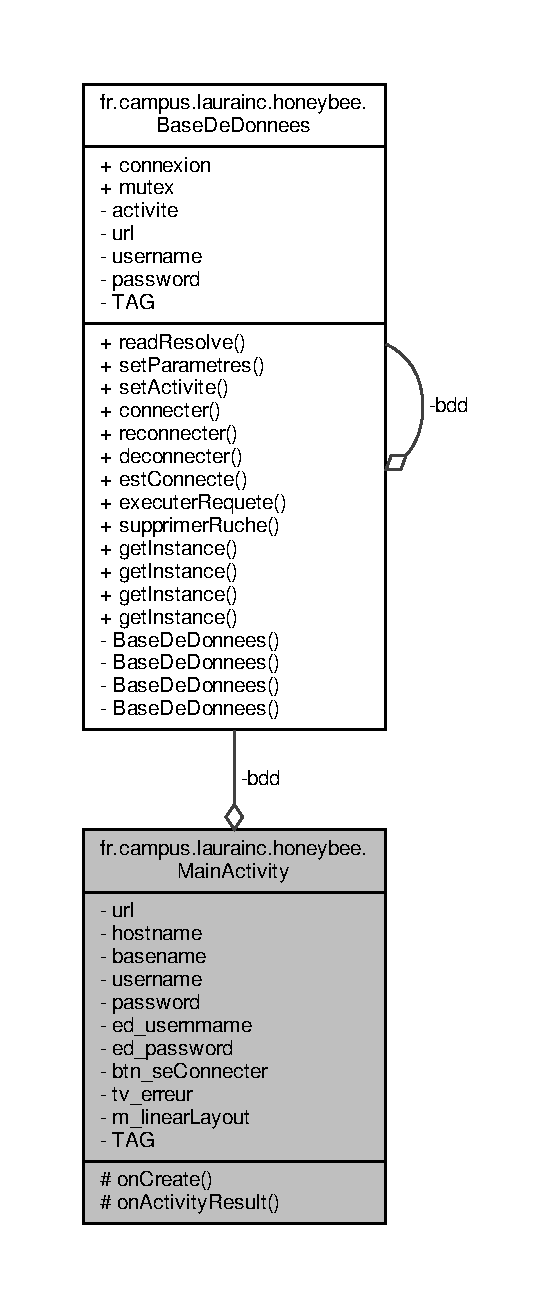
\includegraphics[height=550pt]{classfr_1_1campus_1_1laurainc_1_1honeybee_1_1_main_activity__coll__graph}
\end{center}
\end{figure}
\subsubsection*{Fonctions membres protégées}
\begin{DoxyCompactItemize}
\item 
void \hyperlink{classfr_1_1campus_1_1laurainc_1_1honeybee_1_1_main_activity_aba2e570bbba3bf1be8487068d9c6c2da}{on\+Create} (Bundle saved\+Instance\+State)
\item 
void \hyperlink{classfr_1_1campus_1_1laurainc_1_1honeybee_1_1_main_activity_ae751b46f1881bda6b3b0e08025a9c044}{on\+Activity\+Result} (int request\+Code, int result\+Code, Intent intent)
\end{DoxyCompactItemize}
\subsubsection*{Attributs privés}
\begin{DoxyCompactItemize}
\item 
\hyperlink{classfr_1_1campus_1_1laurainc_1_1honeybee_1_1_base_de_donnees}{Base\+De\+Donnees} \hyperlink{classfr_1_1campus_1_1laurainc_1_1honeybee_1_1_main_activity_ae01aec19dc79f2c48d1807ccb2d3fa4a}{bdd} = null
\begin{DoxyCompactList}\small\item\em l\textquotesingle{}objet permettant un accès à la base de données My\+S\+QL \end{DoxyCompactList}\item 
String \hyperlink{classfr_1_1campus_1_1laurainc_1_1honeybee_1_1_main_activity_adbea1c677048c193ef00a08987905bfa}{url}
\begin{DoxyCompactList}\small\item\em l\textquotesingle{}U\+RL pointant sur la base de données d\textquotesingle{}un serveur My\+S\+QL \end{DoxyCompactList}\item 
String \hyperlink{classfr_1_1campus_1_1laurainc_1_1honeybee_1_1_main_activity_a2d1880e0a470661caaa2610d68299821}{hostname} = \char`\"{}192.\+168.\+52.\+119\char`\"{}
\begin{DoxyCompactList}\small\item\em l\textquotesingle{}adresse IP du serveur My\+S\+QL \end{DoxyCompactList}\item 
String \hyperlink{classfr_1_1campus_1_1laurainc_1_1honeybee_1_1_main_activity_a14d932c5d8ba352ebd01cc984110adf3}{basename} = \char`\"{}ruches\char`\"{}
\begin{DoxyCompactList}\small\item\em le nom de la la base de données du serveur My\+S\+QL \end{DoxyCompactList}\item 
String \hyperlink{classfr_1_1campus_1_1laurainc_1_1honeybee_1_1_main_activity_a1acb2db3f66e167ea225e281d900f842}{username} = \char`\"{}fmellah\char`\"{}
\begin{DoxyCompactList}\small\item\em le nom du compte utilisateur (root par défaut) \end{DoxyCompactList}\item 
String \hyperlink{classfr_1_1campus_1_1laurainc_1_1honeybee_1_1_main_activity_a3cc5f979af0f495f346052f51bd8cd66}{password} = \char`\"{}password\char`\"{}
\begin{DoxyCompactList}\small\item\em le mot de passe du compte utilisateur (password par défaut) \end{DoxyCompactList}\item 
Edit\+Text \hyperlink{classfr_1_1campus_1_1laurainc_1_1honeybee_1_1_main_activity_a6735d2eaf34b76f04b3adbb81d0c9718}{ed\+\_\+usernmame}
\item 
Edit\+Text \hyperlink{classfr_1_1campus_1_1laurainc_1_1honeybee_1_1_main_activity_aba0af7add7bf1a55d54043f88deac4ee}{ed\+\_\+password}
\item 
Button \hyperlink{classfr_1_1campus_1_1laurainc_1_1honeybee_1_1_main_activity_a137abde1340a5e7a9b46decff93ad628}{btn\+\_\+se\+Connecter}
\item 
Text\+View \hyperlink{classfr_1_1campus_1_1laurainc_1_1honeybee_1_1_main_activity_ad36da534773710973fd7696ecc23c117}{tv\+\_\+erreur}
\item 
Linear\+Layout \hyperlink{classfr_1_1campus_1_1laurainc_1_1honeybee_1_1_main_activity_ad042c226bc8ec057b85a3f24ae99777f}{m\+\_\+linear\+Layout}
\end{DoxyCompactItemize}
\subsubsection*{Attributs privés statiques}
\begin{DoxyCompactItemize}
\item 
static final String \hyperlink{classfr_1_1campus_1_1laurainc_1_1honeybee_1_1_main_activity_a70b298f4dd3653ab3d15399d84f96fa9}{T\+AG} = \char`\"{}Main\+Activity\char`\"{}
\begin{DoxyCompactList}\small\item\em le T\+AG de la classe pour les logs \end{DoxyCompactList}\end{DoxyCompactItemize}


\subsubsection{Description détaillée}
\begin{DoxyAuthor}{Auteur}
Clément Laurain 
\end{DoxyAuthor}


\subsubsection{Documentation des fonctions membres}
\mbox{\Hypertarget{classfr_1_1campus_1_1laurainc_1_1honeybee_1_1_main_activity_ae751b46f1881bda6b3b0e08025a9c044}\label{classfr_1_1campus_1_1laurainc_1_1honeybee_1_1_main_activity_ae751b46f1881bda6b3b0e08025a9c044}} 
\index{fr\+::campus\+::laurainc\+::honeybee\+::\+Main\+Activity@{fr\+::campus\+::laurainc\+::honeybee\+::\+Main\+Activity}!on\+Activity\+Result@{on\+Activity\+Result}}
\index{on\+Activity\+Result@{on\+Activity\+Result}!fr\+::campus\+::laurainc\+::honeybee\+::\+Main\+Activity@{fr\+::campus\+::laurainc\+::honeybee\+::\+Main\+Activity}}
\paragraph{\texorpdfstring{on\+Activity\+Result()}{onActivityResult()}}
{\footnotesize\ttfamily fr.\+campus.\+laurainc.\+honeybee.\+Main\+Activity.\+on\+Activity\+Result (\begin{DoxyParamCaption}\item[{int}]{request\+Code,  }\item[{int}]{result\+Code,  }\item[{Intent}]{intent }\end{DoxyParamCaption})\hspace{0.3cm}{\ttfamily [protected]}}

\begin{DoxyRefDesc}{A faire}
\item[\hyperlink{todo__todo000003}{A faire}]Gestion d\textquotesingle{}autres paramètres ? M\+Q\+TT ? ... \end{DoxyRefDesc}


Références \hyperlink{classfr_1_1campus_1_1laurainc_1_1honeybee_1_1_main_activity_a14d932c5d8ba352ebd01cc984110adf3}{fr.\+campus.\+laurainc.\+honeybee.\+Main\+Activity.\+basename}, \hyperlink{classfr_1_1campus_1_1laurainc_1_1honeybee_1_1_honey_bee_a479c42ac63c5c79e26c4836f965171d2}{fr.\+campus.\+laurainc.\+honeybee.\+Honey\+Bee.\+I\+D\+\_\+\+Intent\+\_\+\+Parametres\+Honey\+Bee}, \hyperlink{classfr_1_1campus_1_1laurainc_1_1honeybee_1_1_base_de_donnees_a89357a1cc8a3648400df37a8bfe95958}{fr.\+campus.\+laurainc.\+honeybee.\+Base\+De\+Donnees.\+reconnecter()}, et \hyperlink{classfr_1_1campus_1_1laurainc_1_1honeybee_1_1_base_de_donnees_a0960cb9d71647e80e195a580f90cd0d6}{fr.\+campus.\+laurainc.\+honeybee.\+Base\+De\+Donnees.\+set\+Parametres()}.


\begin{DoxyCode}
00096     \{
00097         \textcolor{comment}{//Log.d(TAG, "requestCode=" + requestCode);}
00098         \textcolor{comment}{//Log.d(TAG, "resultCode=" + resultCode);}
00099         \textcolor{keywordflow}{if} (requestCode == HoneyBee.ID\_Intent\_ParametresHoneyBee)
00100         \{
00101             \textcolor{keywordflow}{switch}(resultCode)
00102             \{
00103                 \textcolor{keywordflow}{case} RESULT\_CANCELED:
00104                     \textcolor{comment}{// rien à faire ?}
00105                     \textcolor{keywordflow}{break};
00106                 \textcolor{keywordflow}{case} RESULT\_OK:
00107                     \textcolor{comment}{// Récupère les paramètres}
00108                     \hyperlink{classfr_1_1campus_1_1laurainc_1_1honeybee_1_1_main_activity_a2d1880e0a470661caaa2610d68299821}{hostname} = intent.getStringExtra(\textcolor{stringliteral}{"hostname"});
00109                     \hyperlink{classfr_1_1campus_1_1laurainc_1_1honeybee_1_1_main_activity_a14d932c5d8ba352ebd01cc984110adf3}{basename} = intent.getStringExtra(\textcolor{stringliteral}{"basename"});
00110                     \hyperlink{classfr_1_1campus_1_1laurainc_1_1honeybee_1_1_main_activity_a1acb2db3f66e167ea225e281d900f842}{username} = intent.getStringExtra(\textcolor{stringliteral}{"username"});
00111                     \hyperlink{classfr_1_1campus_1_1laurainc_1_1honeybee_1_1_main_activity_a3cc5f979af0f495f346052f51bd8cd66}{password} = intent.getStringExtra(\textcolor{stringliteral}{"password"});
00112                     \textcolor{comment}{// Recrée l'URL JDBC MySQL}
00113                     \hyperlink{classfr_1_1campus_1_1laurainc_1_1honeybee_1_1_main_activity_adbea1c677048c193ef00a08987905bfa}{url} = \textcolor{stringliteral}{"jdbc:mysql://"} + \hyperlink{classfr_1_1campus_1_1laurainc_1_1honeybee_1_1_main_activity_a2d1880e0a470661caaa2610d68299821}{hostname} + \textcolor{stringliteral}{"/"} + \hyperlink{classfr_1_1campus_1_1laurainc_1_1honeybee_1_1_main_activity_a14d932c5d8ba352ebd01cc984110adf3}{basename};
00114                     Log.v(\hyperlink{classfr_1_1campus_1_1laurainc_1_1honeybee_1_1_main_activity_a70b298f4dd3653ab3d15399d84f96fa9}{TAG}, \textcolor{stringliteral}{"url="} + \hyperlink{classfr_1_1campus_1_1laurainc_1_1honeybee_1_1_main_activity_adbea1c677048c193ef00a08987905bfa}{url});
00115                     Log.v(\hyperlink{classfr_1_1campus_1_1laurainc_1_1honeybee_1_1_main_activity_a70b298f4dd3653ab3d15399d84f96fa9}{TAG}, \textcolor{stringliteral}{"username="} + \hyperlink{classfr_1_1campus_1_1laurainc_1_1honeybee_1_1_main_activity_a1acb2db3f66e167ea225e281d900f842}{username});
00116                     Log.v(\hyperlink{classfr_1_1campus_1_1laurainc_1_1honeybee_1_1_main_activity_a70b298f4dd3653ab3d15399d84f96fa9}{TAG}, \textcolor{stringliteral}{"password="} + \hyperlink{classfr_1_1campus_1_1laurainc_1_1honeybee_1_1_main_activity_a3cc5f979af0f495f346052f51bd8cd66}{password});
00117                     \hyperlink{classfr_1_1campus_1_1laurainc_1_1honeybee_1_1_main_activity_ae01aec19dc79f2c48d1807ccb2d3fa4a}{bdd}.\hyperlink{classfr_1_1campus_1_1laurainc_1_1honeybee_1_1_base_de_donnees_a0960cb9d71647e80e195a580f90cd0d6}{setParametres}(\hyperlink{classfr_1_1campus_1_1laurainc_1_1honeybee_1_1_main_activity_adbea1c677048c193ef00a08987905bfa}{url}, \hyperlink{classfr_1_1campus_1_1laurainc_1_1honeybee_1_1_main_activity_a1acb2db3f66e167ea225e281d900f842}{username}, 
      \hyperlink{classfr_1_1campus_1_1laurainc_1_1honeybee_1_1_main_activity_a3cc5f979af0f495f346052f51bd8cd66}{password});
00118                     \hyperlink{classfr_1_1campus_1_1laurainc_1_1honeybee_1_1_main_activity_ae01aec19dc79f2c48d1807ccb2d3fa4a}{bdd}.\hyperlink{classfr_1_1campus_1_1laurainc_1_1honeybee_1_1_base_de_donnees_a89357a1cc8a3648400df37a8bfe95958}{reconnecter}();
00119 
00123                     \textcolor{keywordflow}{break};
00124             \}
00125         \}
00126     \}
\end{DoxyCode}
\mbox{\Hypertarget{classfr_1_1campus_1_1laurainc_1_1honeybee_1_1_main_activity_aba2e570bbba3bf1be8487068d9c6c2da}\label{classfr_1_1campus_1_1laurainc_1_1honeybee_1_1_main_activity_aba2e570bbba3bf1be8487068d9c6c2da}} 
\index{fr\+::campus\+::laurainc\+::honeybee\+::\+Main\+Activity@{fr\+::campus\+::laurainc\+::honeybee\+::\+Main\+Activity}!on\+Create@{on\+Create}}
\index{on\+Create@{on\+Create}!fr\+::campus\+::laurainc\+::honeybee\+::\+Main\+Activity@{fr\+::campus\+::laurainc\+::honeybee\+::\+Main\+Activity}}
\paragraph{\texorpdfstring{on\+Create()}{onCreate()}}
{\footnotesize\ttfamily void fr.\+campus.\+laurainc.\+honeybee.\+Main\+Activity.\+on\+Create (\begin{DoxyParamCaption}\item[{Bundle}]{saved\+Instance\+State }\end{DoxyParamCaption})\hspace{0.3cm}{\ttfamily [protected]}}

\begin{DoxyRefDesc}{A faire}
\item[\hyperlink{todo__todo000002}{A faire}]Affichage de l\textquotesingle{}état de connexion My\+S\+QL ? \end{DoxyRefDesc}


Références \hyperlink{classfr_1_1campus_1_1laurainc_1_1honeybee_1_1_main_activity_a14d932c5d8ba352ebd01cc984110adf3}{fr.\+campus.\+laurainc.\+honeybee.\+Main\+Activity.\+basename}, \hyperlink{classfr_1_1campus_1_1laurainc_1_1honeybee_1_1_base_de_donnees_a08564ea7dccde161d6eac4b8879401bb}{fr.\+campus.\+laurainc.\+honeybee.\+Base\+De\+Donnees.\+connecter()}, et \hyperlink{classfr_1_1campus_1_1laurainc_1_1honeybee_1_1_base_de_donnees_a9c2484cfb87f90e46cf878eb7803abb2}{fr.\+campus.\+laurainc.\+honeybee.\+Base\+De\+Donnees.\+get\+Instance()}.


\begin{DoxyCode}
00040     \{
00041         super.onCreate(savedInstanceState);
00042         setContentView(R.layout.activity\_main);
00043 
00044         \hyperlink{classfr_1_1campus_1_1laurainc_1_1honeybee_1_1_main_activity_a6735d2eaf34b76f04b3adbb81d0c9718}{ed\_usernmame} = findViewById(R.id.ed\_username);
00045         \hyperlink{classfr_1_1campus_1_1laurainc_1_1honeybee_1_1_main_activity_aba0af7add7bf1a55d54043f88deac4ee}{ed\_password} = findViewById(R.id.ed\_password);
00046         \hyperlink{classfr_1_1campus_1_1laurainc_1_1honeybee_1_1_main_activity_a137abde1340a5e7a9b46decff93ad628}{btn\_seConnecter} = findViewById(R.id.btn\_seConnecter);
00047         \hyperlink{classfr_1_1campus_1_1laurainc_1_1honeybee_1_1_main_activity_ad36da534773710973fd7696ecc23c117}{tv\_erreur} = findViewById(R.id.tv\_erreur);
00048 
00049         \textcolor{comment}{// Initialise l'url pour la connexion à la base de données MySQL}
00050         \hyperlink{classfr_1_1campus_1_1laurainc_1_1honeybee_1_1_main_activity_adbea1c677048c193ef00a08987905bfa}{url} = \textcolor{stringliteral}{"jdbc:mysql://"} + \hyperlink{classfr_1_1campus_1_1laurainc_1_1honeybee_1_1_main_activity_a2d1880e0a470661caaa2610d68299821}{hostname} + \textcolor{stringliteral}{"/"} + \hyperlink{classfr_1_1campus_1_1laurainc_1_1honeybee_1_1_main_activity_a14d932c5d8ba352ebd01cc984110adf3}{basename};
00051         \textcolor{comment}{// Récupère l'instance de BaseDeDonnees}
00052         \hyperlink{classfr_1_1campus_1_1laurainc_1_1honeybee_1_1_main_activity_ae01aec19dc79f2c48d1807ccb2d3fa4a}{bdd} = \hyperlink{class_base_de_donnees}{BaseDeDonnees}.\hyperlink{class_base_de_donnees_a80028aa2b6b4fbf30fb2e36357b7d3d3}{getInstance}(\textcolor{keyword}{this}, \hyperlink{classfr_1_1campus_1_1laurainc_1_1honeybee_1_1_main_activity_adbea1c677048c193ef00a08987905bfa}{url}, 
      \hyperlink{classfr_1_1campus_1_1laurainc_1_1honeybee_1_1_main_activity_a1acb2db3f66e167ea225e281d900f842}{username}, \hyperlink{classfr_1_1campus_1_1laurainc_1_1honeybee_1_1_main_activity_a3cc5f979af0f495f346052f51bd8cd66}{password});
00053         \hyperlink{classfr_1_1campus_1_1laurainc_1_1honeybee_1_1_main_activity_ae01aec19dc79f2c48d1807ccb2d3fa4a}{bdd}.\hyperlink{classfr_1_1campus_1_1laurainc_1_1honeybee_1_1_base_de_donnees_a08564ea7dccde161d6eac4b8879401bb}{connecter}();
00057 
00058         \textcolor{comment}{// Fenêtre d'accès aux ruches}
00059         \textcolor{keyword}{final} Intent homeActivity = \textcolor{keyword}{new} Intent(MainActivity.this, homeActivity.class);
00060        \hyperlink{classfr_1_1campus_1_1laurainc_1_1honeybee_1_1_main_activity_a137abde1340a5e7a9b46decff93ad628}{btn\_seConnecter}.setOnClickListener(\textcolor{keyword}{new} View.OnClickListener() \{
00061            @Override
00062            \textcolor{keyword}{public} \textcolor{keywordtype}{void} onClick(View v) \{
00063                \textcolor{keywordflow}{if}(\hyperlink{classfr_1_1campus_1_1laurainc_1_1honeybee_1_1_main_activity_a6735d2eaf34b76f04b3adbb81d0c9718}{ed\_usernmame}.getText().toString().equals(\hyperlink{classfr_1_1campus_1_1laurainc_1_1honeybee_1_1_main_activity_a1acb2db3f66e167ea225e281d900f842}{username}) && 
      \hyperlink{classfr_1_1campus_1_1laurainc_1_1honeybee_1_1_main_activity_aba0af7add7bf1a55d54043f88deac4ee}{ed\_password}.getText().toString().equals((\hyperlink{classfr_1_1campus_1_1laurainc_1_1honeybee_1_1_main_activity_a3cc5f979af0f495f346052f51bd8cd66}{password})))
00064                \{
00065                    startActivity(homeActivity);
00066                \}
00067                \textcolor{keywordflow}{else}
00068                \{
00069                     \hyperlink{classfr_1_1campus_1_1laurainc_1_1honeybee_1_1_main_activity_ad36da534773710973fd7696ecc23c117}{tv\_erreur}.setVisibility(View.VISIBLE);
00070                \}
00071            \}
00072        \});
00073 
00074         \textcolor{comment}{// Fenêtre de paramétrage de l'application}
00075         \textcolor{comment}{/*FloatingActionButton btn\_Parametres = findViewById(R.id.btn\_Parametres);
}
00076 \textcolor{comment}{        btn\_Parametres.setOnClickListener(new View.OnClickListener() \{
}
00077 \textcolor{comment}{            public void onClick(View v) \{
}
00078 \textcolor{comment}{                // Crée et démarre une activité
}
00079 \textcolor{comment}{                Intent intent = new Intent(MainActivity.this, ParametresHoneyBeeActivity.class);
}
00080 \textcolor{comment}{                // Passage de données
}
00081 \textcolor{comment}{                intent.putExtra("hostname", hostname);
}
00082 \textcolor{comment}{                intent.putExtra("basename", basename);
}
00083 \textcolor{comment}{                intent.putExtra("username", username);
}
00084 \textcolor{comment}{                intent.putExtra("password", password);
}
00085 \textcolor{comment}{                //startActivity(intent);
}
00086 \textcolor{comment}{                startActivityForResult(intent, HoneyBee.ID\_Intent\_ParametresHoneyBee);
}
00087 \textcolor{comment}{            \}
}
00088 \textcolor{comment}{        \});*/}
00089     \}
\end{DoxyCode}


\subsubsection{Documentation des données membres}
\mbox{\Hypertarget{classfr_1_1campus_1_1laurainc_1_1honeybee_1_1_main_activity_a14d932c5d8ba352ebd01cc984110adf3}\label{classfr_1_1campus_1_1laurainc_1_1honeybee_1_1_main_activity_a14d932c5d8ba352ebd01cc984110adf3}} 
\index{fr\+::campus\+::laurainc\+::honeybee\+::\+Main\+Activity@{fr\+::campus\+::laurainc\+::honeybee\+::\+Main\+Activity}!basename@{basename}}
\index{basename@{basename}!fr\+::campus\+::laurainc\+::honeybee\+::\+Main\+Activity@{fr\+::campus\+::laurainc\+::honeybee\+::\+Main\+Activity}}
\paragraph{\texorpdfstring{basename}{basename}}
{\footnotesize\ttfamily String fr.\+campus.\+laurainc.\+honeybee.\+Main\+Activity.\+basename = \char`\"{}ruches\char`\"{}\hspace{0.3cm}{\ttfamily [private]}}



Référencé par \hyperlink{classfr_1_1campus_1_1laurainc_1_1honeybee_1_1_main_activity_ae751b46f1881bda6b3b0e08025a9c044}{fr.\+campus.\+laurainc.\+honeybee.\+Main\+Activity.\+on\+Activity\+Result()}, et \hyperlink{classfr_1_1campus_1_1laurainc_1_1honeybee_1_1_main_activity_aba2e570bbba3bf1be8487068d9c6c2da}{fr.\+campus.\+laurainc.\+honeybee.\+Main\+Activity.\+on\+Create()}.

\mbox{\Hypertarget{classfr_1_1campus_1_1laurainc_1_1honeybee_1_1_main_activity_ae01aec19dc79f2c48d1807ccb2d3fa4a}\label{classfr_1_1campus_1_1laurainc_1_1honeybee_1_1_main_activity_ae01aec19dc79f2c48d1807ccb2d3fa4a}} 
\index{fr\+::campus\+::laurainc\+::honeybee\+::\+Main\+Activity@{fr\+::campus\+::laurainc\+::honeybee\+::\+Main\+Activity}!bdd@{bdd}}
\index{bdd@{bdd}!fr\+::campus\+::laurainc\+::honeybee\+::\+Main\+Activity@{fr\+::campus\+::laurainc\+::honeybee\+::\+Main\+Activity}}
\paragraph{\texorpdfstring{bdd}{bdd}}
{\footnotesize\ttfamily \hyperlink{classfr_1_1campus_1_1laurainc_1_1honeybee_1_1_base_de_donnees}{Base\+De\+Donnees} fr.\+campus.\+laurainc.\+honeybee.\+Main\+Activity.\+bdd = null\hspace{0.3cm}{\ttfamily [private]}}

\mbox{\Hypertarget{classfr_1_1campus_1_1laurainc_1_1honeybee_1_1_main_activity_a137abde1340a5e7a9b46decff93ad628}\label{classfr_1_1campus_1_1laurainc_1_1honeybee_1_1_main_activity_a137abde1340a5e7a9b46decff93ad628}} 
\index{fr\+::campus\+::laurainc\+::honeybee\+::\+Main\+Activity@{fr\+::campus\+::laurainc\+::honeybee\+::\+Main\+Activity}!btn\+\_\+se\+Connecter@{btn\+\_\+se\+Connecter}}
\index{btn\+\_\+se\+Connecter@{btn\+\_\+se\+Connecter}!fr\+::campus\+::laurainc\+::honeybee\+::\+Main\+Activity@{fr\+::campus\+::laurainc\+::honeybee\+::\+Main\+Activity}}
\paragraph{\texorpdfstring{btn\+\_\+se\+Connecter}{btn\_seConnecter}}
{\footnotesize\ttfamily Button fr.\+campus.\+laurainc.\+honeybee.\+Main\+Activity.\+btn\+\_\+se\+Connecter\hspace{0.3cm}{\ttfamily [private]}}

\mbox{\Hypertarget{classfr_1_1campus_1_1laurainc_1_1honeybee_1_1_main_activity_aba0af7add7bf1a55d54043f88deac4ee}\label{classfr_1_1campus_1_1laurainc_1_1honeybee_1_1_main_activity_aba0af7add7bf1a55d54043f88deac4ee}} 
\index{fr\+::campus\+::laurainc\+::honeybee\+::\+Main\+Activity@{fr\+::campus\+::laurainc\+::honeybee\+::\+Main\+Activity}!ed\+\_\+password@{ed\+\_\+password}}
\index{ed\+\_\+password@{ed\+\_\+password}!fr\+::campus\+::laurainc\+::honeybee\+::\+Main\+Activity@{fr\+::campus\+::laurainc\+::honeybee\+::\+Main\+Activity}}
\paragraph{\texorpdfstring{ed\+\_\+password}{ed\_password}}
{\footnotesize\ttfamily Edit\+Text fr.\+campus.\+laurainc.\+honeybee.\+Main\+Activity.\+ed\+\_\+password\hspace{0.3cm}{\ttfamily [private]}}

\mbox{\Hypertarget{classfr_1_1campus_1_1laurainc_1_1honeybee_1_1_main_activity_a6735d2eaf34b76f04b3adbb81d0c9718}\label{classfr_1_1campus_1_1laurainc_1_1honeybee_1_1_main_activity_a6735d2eaf34b76f04b3adbb81d0c9718}} 
\index{fr\+::campus\+::laurainc\+::honeybee\+::\+Main\+Activity@{fr\+::campus\+::laurainc\+::honeybee\+::\+Main\+Activity}!ed\+\_\+usernmame@{ed\+\_\+usernmame}}
\index{ed\+\_\+usernmame@{ed\+\_\+usernmame}!fr\+::campus\+::laurainc\+::honeybee\+::\+Main\+Activity@{fr\+::campus\+::laurainc\+::honeybee\+::\+Main\+Activity}}
\paragraph{\texorpdfstring{ed\+\_\+usernmame}{ed\_usernmame}}
{\footnotesize\ttfamily Edit\+Text fr.\+campus.\+laurainc.\+honeybee.\+Main\+Activity.\+ed\+\_\+usernmame\hspace{0.3cm}{\ttfamily [private]}}

\mbox{\Hypertarget{classfr_1_1campus_1_1laurainc_1_1honeybee_1_1_main_activity_a2d1880e0a470661caaa2610d68299821}\label{classfr_1_1campus_1_1laurainc_1_1honeybee_1_1_main_activity_a2d1880e0a470661caaa2610d68299821}} 
\index{fr\+::campus\+::laurainc\+::honeybee\+::\+Main\+Activity@{fr\+::campus\+::laurainc\+::honeybee\+::\+Main\+Activity}!hostname@{hostname}}
\index{hostname@{hostname}!fr\+::campus\+::laurainc\+::honeybee\+::\+Main\+Activity@{fr\+::campus\+::laurainc\+::honeybee\+::\+Main\+Activity}}
\paragraph{\texorpdfstring{hostname}{hostname}}
{\footnotesize\ttfamily String fr.\+campus.\+laurainc.\+honeybee.\+Main\+Activity.\+hostname = \char`\"{}192.\+168.\+52.\+119\char`\"{}\hspace{0.3cm}{\ttfamily [private]}}

\mbox{\Hypertarget{classfr_1_1campus_1_1laurainc_1_1honeybee_1_1_main_activity_ad042c226bc8ec057b85a3f24ae99777f}\label{classfr_1_1campus_1_1laurainc_1_1honeybee_1_1_main_activity_ad042c226bc8ec057b85a3f24ae99777f}} 
\index{fr\+::campus\+::laurainc\+::honeybee\+::\+Main\+Activity@{fr\+::campus\+::laurainc\+::honeybee\+::\+Main\+Activity}!m\+\_\+linear\+Layout@{m\+\_\+linear\+Layout}}
\index{m\+\_\+linear\+Layout@{m\+\_\+linear\+Layout}!fr\+::campus\+::laurainc\+::honeybee\+::\+Main\+Activity@{fr\+::campus\+::laurainc\+::honeybee\+::\+Main\+Activity}}
\paragraph{\texorpdfstring{m\+\_\+linear\+Layout}{m\_linearLayout}}
{\footnotesize\ttfamily Linear\+Layout fr.\+campus.\+laurainc.\+honeybee.\+Main\+Activity.\+m\+\_\+linear\+Layout\hspace{0.3cm}{\ttfamily [private]}}

\mbox{\Hypertarget{classfr_1_1campus_1_1laurainc_1_1honeybee_1_1_main_activity_a3cc5f979af0f495f346052f51bd8cd66}\label{classfr_1_1campus_1_1laurainc_1_1honeybee_1_1_main_activity_a3cc5f979af0f495f346052f51bd8cd66}} 
\index{fr\+::campus\+::laurainc\+::honeybee\+::\+Main\+Activity@{fr\+::campus\+::laurainc\+::honeybee\+::\+Main\+Activity}!password@{password}}
\index{password@{password}!fr\+::campus\+::laurainc\+::honeybee\+::\+Main\+Activity@{fr\+::campus\+::laurainc\+::honeybee\+::\+Main\+Activity}}
\paragraph{\texorpdfstring{password}{password}}
{\footnotesize\ttfamily String fr.\+campus.\+laurainc.\+honeybee.\+Main\+Activity.\+password = \char`\"{}password\char`\"{}\hspace{0.3cm}{\ttfamily [private]}}

\mbox{\Hypertarget{classfr_1_1campus_1_1laurainc_1_1honeybee_1_1_main_activity_a70b298f4dd3653ab3d15399d84f96fa9}\label{classfr_1_1campus_1_1laurainc_1_1honeybee_1_1_main_activity_a70b298f4dd3653ab3d15399d84f96fa9}} 
\index{fr\+::campus\+::laurainc\+::honeybee\+::\+Main\+Activity@{fr\+::campus\+::laurainc\+::honeybee\+::\+Main\+Activity}!T\+AG@{T\+AG}}
\index{T\+AG@{T\+AG}!fr\+::campus\+::laurainc\+::honeybee\+::\+Main\+Activity@{fr\+::campus\+::laurainc\+::honeybee\+::\+Main\+Activity}}
\paragraph{\texorpdfstring{T\+AG}{TAG}}
{\footnotesize\ttfamily final String fr.\+campus.\+laurainc.\+honeybee.\+Main\+Activity.\+T\+AG = \char`\"{}Main\+Activity\char`\"{}\hspace{0.3cm}{\ttfamily [static]}, {\ttfamily [private]}}

\mbox{\Hypertarget{classfr_1_1campus_1_1laurainc_1_1honeybee_1_1_main_activity_ad36da534773710973fd7696ecc23c117}\label{classfr_1_1campus_1_1laurainc_1_1honeybee_1_1_main_activity_ad36da534773710973fd7696ecc23c117}} 
\index{fr\+::campus\+::laurainc\+::honeybee\+::\+Main\+Activity@{fr\+::campus\+::laurainc\+::honeybee\+::\+Main\+Activity}!tv\+\_\+erreur@{tv\+\_\+erreur}}
\index{tv\+\_\+erreur@{tv\+\_\+erreur}!fr\+::campus\+::laurainc\+::honeybee\+::\+Main\+Activity@{fr\+::campus\+::laurainc\+::honeybee\+::\+Main\+Activity}}
\paragraph{\texorpdfstring{tv\+\_\+erreur}{tv\_erreur}}
{\footnotesize\ttfamily Text\+View fr.\+campus.\+laurainc.\+honeybee.\+Main\+Activity.\+tv\+\_\+erreur\hspace{0.3cm}{\ttfamily [private]}}

\mbox{\Hypertarget{classfr_1_1campus_1_1laurainc_1_1honeybee_1_1_main_activity_adbea1c677048c193ef00a08987905bfa}\label{classfr_1_1campus_1_1laurainc_1_1honeybee_1_1_main_activity_adbea1c677048c193ef00a08987905bfa}} 
\index{fr\+::campus\+::laurainc\+::honeybee\+::\+Main\+Activity@{fr\+::campus\+::laurainc\+::honeybee\+::\+Main\+Activity}!url@{url}}
\index{url@{url}!fr\+::campus\+::laurainc\+::honeybee\+::\+Main\+Activity@{fr\+::campus\+::laurainc\+::honeybee\+::\+Main\+Activity}}
\paragraph{\texorpdfstring{url}{url}}
{\footnotesize\ttfamily String fr.\+campus.\+laurainc.\+honeybee.\+Main\+Activity.\+url\hspace{0.3cm}{\ttfamily [private]}}

\mbox{\Hypertarget{classfr_1_1campus_1_1laurainc_1_1honeybee_1_1_main_activity_a1acb2db3f66e167ea225e281d900f842}\label{classfr_1_1campus_1_1laurainc_1_1honeybee_1_1_main_activity_a1acb2db3f66e167ea225e281d900f842}} 
\index{fr\+::campus\+::laurainc\+::honeybee\+::\+Main\+Activity@{fr\+::campus\+::laurainc\+::honeybee\+::\+Main\+Activity}!username@{username}}
\index{username@{username}!fr\+::campus\+::laurainc\+::honeybee\+::\+Main\+Activity@{fr\+::campus\+::laurainc\+::honeybee\+::\+Main\+Activity}}
\paragraph{\texorpdfstring{username}{username}}
{\footnotesize\ttfamily String fr.\+campus.\+laurainc.\+honeybee.\+Main\+Activity.\+username = \char`\"{}fmellah\char`\"{}\hspace{0.3cm}{\ttfamily [private]}}



La documentation de cette classe a été générée à partir du fichier suivant \+:\begin{DoxyCompactItemize}
\item 
\hyperlink{_main_activity_8java}{Main\+Activity.\+java}\end{DoxyCompactItemize}

\hypertarget{struct_mesure_horaire_environement}{}\subsection{Référence de la structure Mesure\+Horaire\+Environement}
\label{struct_mesure_horaire_environement}\index{Mesure\+Horaire\+Environement@{Mesure\+Horaire\+Environement}}


structure de données pour les mesures horaires  




{\ttfamily \#include $<$ruche.\+h$>$}



Graphe de collaboration de Mesure\+Horaire\+Environement\+:\nopagebreak
\begin{figure}[H]
\begin{center}
\leavevmode
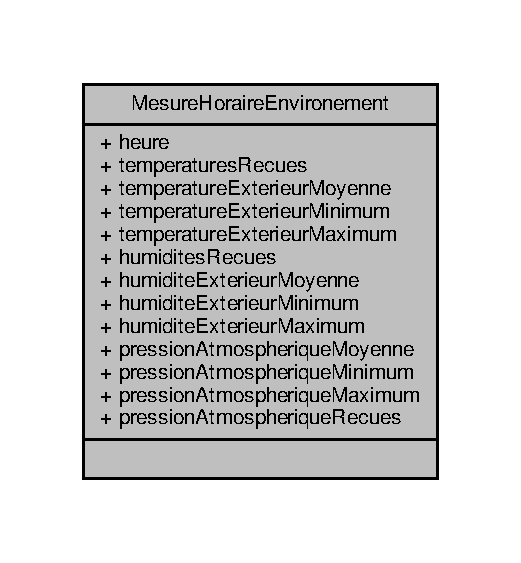
\includegraphics[width=250pt]{struct_mesure_horaire_environement__coll__graph}
\end{center}
\end{figure}
\subsubsection*{Attributs publics}
\begin{DoxyCompactItemize}
\item 
int \hyperlink{struct_mesure_horaire_environement_a83295c95940d9edae2d082a94f49e1c9}{heure}
\item 
bool \hyperlink{struct_mesure_horaire_environement_a3444440b836c4893e8d61c3eb5c3e42d}{temperatures\+Recues} = false
\item 
double \hyperlink{struct_mesure_horaire_environement_a40be086e9b2454c0e70066a523a1b066}{temperature\+Exterieur\+Moyenne}
\item 
double \hyperlink{struct_mesure_horaire_environement_ae9737a62128ecf2614901ebe0b118548}{temperature\+Exterieur\+Minimum}
\item 
double \hyperlink{struct_mesure_horaire_environement_aaf73ec5bb5a7c8235c56dc4ea3c4d89c}{temperature\+Exterieur\+Maximum}
\item 
bool \hyperlink{struct_mesure_horaire_environement_a4348771984d70b9ea7867dba511db336}{humidites\+Recues} = false
\item 
double \hyperlink{struct_mesure_horaire_environement_a25909e0885ee3588c637b738ced303d7}{humidite\+Exterieur\+Moyenne}
\item 
double \hyperlink{struct_mesure_horaire_environement_a1621bd692dc352708d1931a48df9a596}{humidite\+Exterieur\+Minimum}
\item 
double \hyperlink{struct_mesure_horaire_environement_abb2c00c4262837d9e1122573283d86ec}{humidite\+Exterieur\+Maximum}
\item 
double \hyperlink{struct_mesure_horaire_environement_a6ae12cb9b6ac6a46f7c08e60049c7b72}{pression\+Atmospherique\+Moyenne}
\item 
double \hyperlink{struct_mesure_horaire_environement_a3d42b48772717461f7395cdae5ff925f}{pression\+Atmospherique\+Minimum}
\item 
double \hyperlink{struct_mesure_horaire_environement_a9b82da49ea52c6f118f25433a16e22d4}{pression\+Atmospherique\+Maximum}
\item 
bool \hyperlink{struct_mesure_horaire_environement_a5db5e56af7d297b500912489126f7305}{pression\+Atmospherique\+Recues} = false
\end{DoxyCompactItemize}


\subsubsection{Description détaillée}
\begin{DoxyAuthor}{Auteur}
Florentin Mellah, Enzo Rossi
\end{DoxyAuthor}
\begin{DoxyVersion}{Version}
1.\+1 
\end{DoxyVersion}


\subsubsection{Documentation des données membres}
\mbox{\Hypertarget{struct_mesure_horaire_environement_a83295c95940d9edae2d082a94f49e1c9}\label{struct_mesure_horaire_environement_a83295c95940d9edae2d082a94f49e1c9}} 
\index{Mesure\+Horaire\+Environement@{Mesure\+Horaire\+Environement}!heure@{heure}}
\index{heure@{heure}!Mesure\+Horaire\+Environement@{Mesure\+Horaire\+Environement}}
\paragraph{\texorpdfstring{heure}{heure}}
{\footnotesize\ttfamily int Mesure\+Horaire\+Environement\+::heure}



Référencé par \hyperlink{class_ruche_ac52e79446c5629645e02e27d2a01e56c}{Ruche\+::inserer\+Mesure\+Horaire\+Environnement()}, \hyperlink{class_ruche_a59e89246b484d7b63851c0ebd20af6c5}{Ruche\+::recevoir\+Traitement\+Humidite\+Exterieur()}, \hyperlink{class_ruche_aa42daeffa023c83fde40072601e1fa39}{Ruche\+::recevoir\+Traitement\+Pression\+Atmospherique()}, et \hyperlink{class_ruche_a8482dda95a8a7888d5a60ea6f7d8729e}{Ruche\+::recevoir\+Traitement\+Temperature\+Exterieur()}.

\mbox{\Hypertarget{struct_mesure_horaire_environement_abb2c00c4262837d9e1122573283d86ec}\label{struct_mesure_horaire_environement_abb2c00c4262837d9e1122573283d86ec}} 
\index{Mesure\+Horaire\+Environement@{Mesure\+Horaire\+Environement}!humidite\+Exterieur\+Maximum@{humidite\+Exterieur\+Maximum}}
\index{humidite\+Exterieur\+Maximum@{humidite\+Exterieur\+Maximum}!Mesure\+Horaire\+Environement@{Mesure\+Horaire\+Environement}}
\paragraph{\texorpdfstring{humidite\+Exterieur\+Maximum}{humiditeExterieurMaximum}}
{\footnotesize\ttfamily double Mesure\+Horaire\+Environement\+::humidite\+Exterieur\+Maximum}



Référencé par \hyperlink{class_ruche_ac52e79446c5629645e02e27d2a01e56c}{Ruche\+::inserer\+Mesure\+Horaire\+Environnement()}, et \hyperlink{class_ruche_a59e89246b484d7b63851c0ebd20af6c5}{Ruche\+::recevoir\+Traitement\+Humidite\+Exterieur()}.

\mbox{\Hypertarget{struct_mesure_horaire_environement_a1621bd692dc352708d1931a48df9a596}\label{struct_mesure_horaire_environement_a1621bd692dc352708d1931a48df9a596}} 
\index{Mesure\+Horaire\+Environement@{Mesure\+Horaire\+Environement}!humidite\+Exterieur\+Minimum@{humidite\+Exterieur\+Minimum}}
\index{humidite\+Exterieur\+Minimum@{humidite\+Exterieur\+Minimum}!Mesure\+Horaire\+Environement@{Mesure\+Horaire\+Environement}}
\paragraph{\texorpdfstring{humidite\+Exterieur\+Minimum}{humiditeExterieurMinimum}}
{\footnotesize\ttfamily double Mesure\+Horaire\+Environement\+::humidite\+Exterieur\+Minimum}



Référencé par \hyperlink{class_ruche_ac52e79446c5629645e02e27d2a01e56c}{Ruche\+::inserer\+Mesure\+Horaire\+Environnement()}, et \hyperlink{class_ruche_a59e89246b484d7b63851c0ebd20af6c5}{Ruche\+::recevoir\+Traitement\+Humidite\+Exterieur()}.

\mbox{\Hypertarget{struct_mesure_horaire_environement_a25909e0885ee3588c637b738ced303d7}\label{struct_mesure_horaire_environement_a25909e0885ee3588c637b738ced303d7}} 
\index{Mesure\+Horaire\+Environement@{Mesure\+Horaire\+Environement}!humidite\+Exterieur\+Moyenne@{humidite\+Exterieur\+Moyenne}}
\index{humidite\+Exterieur\+Moyenne@{humidite\+Exterieur\+Moyenne}!Mesure\+Horaire\+Environement@{Mesure\+Horaire\+Environement}}
\paragraph{\texorpdfstring{humidite\+Exterieur\+Moyenne}{humiditeExterieurMoyenne}}
{\footnotesize\ttfamily double Mesure\+Horaire\+Environement\+::humidite\+Exterieur\+Moyenne}



Référencé par \hyperlink{class_ruche_ac52e79446c5629645e02e27d2a01e56c}{Ruche\+::inserer\+Mesure\+Horaire\+Environnement()}, et \hyperlink{class_ruche_a59e89246b484d7b63851c0ebd20af6c5}{Ruche\+::recevoir\+Traitement\+Humidite\+Exterieur()}.

\mbox{\Hypertarget{struct_mesure_horaire_environement_a4348771984d70b9ea7867dba511db336}\label{struct_mesure_horaire_environement_a4348771984d70b9ea7867dba511db336}} 
\index{Mesure\+Horaire\+Environement@{Mesure\+Horaire\+Environement}!humidites\+Recues@{humidites\+Recues}}
\index{humidites\+Recues@{humidites\+Recues}!Mesure\+Horaire\+Environement@{Mesure\+Horaire\+Environement}}
\paragraph{\texorpdfstring{humidites\+Recues}{humiditesRecues}}
{\footnotesize\ttfamily bool Mesure\+Horaire\+Environement\+::humidites\+Recues = false}



Référencé par \hyperlink{class_ruche_ac52e79446c5629645e02e27d2a01e56c}{Ruche\+::inserer\+Mesure\+Horaire\+Environnement()}, et \hyperlink{class_ruche_a59e89246b484d7b63851c0ebd20af6c5}{Ruche\+::recevoir\+Traitement\+Humidite\+Exterieur()}.

\mbox{\Hypertarget{struct_mesure_horaire_environement_a9b82da49ea52c6f118f25433a16e22d4}\label{struct_mesure_horaire_environement_a9b82da49ea52c6f118f25433a16e22d4}} 
\index{Mesure\+Horaire\+Environement@{Mesure\+Horaire\+Environement}!pression\+Atmospherique\+Maximum@{pression\+Atmospherique\+Maximum}}
\index{pression\+Atmospherique\+Maximum@{pression\+Atmospherique\+Maximum}!Mesure\+Horaire\+Environement@{Mesure\+Horaire\+Environement}}
\paragraph{\texorpdfstring{pression\+Atmospherique\+Maximum}{pressionAtmospheriqueMaximum}}
{\footnotesize\ttfamily double Mesure\+Horaire\+Environement\+::pression\+Atmospherique\+Maximum}



Référencé par \hyperlink{class_ruche_ac52e79446c5629645e02e27d2a01e56c}{Ruche\+::inserer\+Mesure\+Horaire\+Environnement()}, et \hyperlink{class_ruche_aa42daeffa023c83fde40072601e1fa39}{Ruche\+::recevoir\+Traitement\+Pression\+Atmospherique()}.

\mbox{\Hypertarget{struct_mesure_horaire_environement_a3d42b48772717461f7395cdae5ff925f}\label{struct_mesure_horaire_environement_a3d42b48772717461f7395cdae5ff925f}} 
\index{Mesure\+Horaire\+Environement@{Mesure\+Horaire\+Environement}!pression\+Atmospherique\+Minimum@{pression\+Atmospherique\+Minimum}}
\index{pression\+Atmospherique\+Minimum@{pression\+Atmospherique\+Minimum}!Mesure\+Horaire\+Environement@{Mesure\+Horaire\+Environement}}
\paragraph{\texorpdfstring{pression\+Atmospherique\+Minimum}{pressionAtmospheriqueMinimum}}
{\footnotesize\ttfamily double Mesure\+Horaire\+Environement\+::pression\+Atmospherique\+Minimum}



Référencé par \hyperlink{class_ruche_ac52e79446c5629645e02e27d2a01e56c}{Ruche\+::inserer\+Mesure\+Horaire\+Environnement()}, et \hyperlink{class_ruche_aa42daeffa023c83fde40072601e1fa39}{Ruche\+::recevoir\+Traitement\+Pression\+Atmospherique()}.

\mbox{\Hypertarget{struct_mesure_horaire_environement_a6ae12cb9b6ac6a46f7c08e60049c7b72}\label{struct_mesure_horaire_environement_a6ae12cb9b6ac6a46f7c08e60049c7b72}} 
\index{Mesure\+Horaire\+Environement@{Mesure\+Horaire\+Environement}!pression\+Atmospherique\+Moyenne@{pression\+Atmospherique\+Moyenne}}
\index{pression\+Atmospherique\+Moyenne@{pression\+Atmospherique\+Moyenne}!Mesure\+Horaire\+Environement@{Mesure\+Horaire\+Environement}}
\paragraph{\texorpdfstring{pression\+Atmospherique\+Moyenne}{pressionAtmospheriqueMoyenne}}
{\footnotesize\ttfamily double Mesure\+Horaire\+Environement\+::pression\+Atmospherique\+Moyenne}



Référencé par \hyperlink{class_ruche_ac52e79446c5629645e02e27d2a01e56c}{Ruche\+::inserer\+Mesure\+Horaire\+Environnement()}, et \hyperlink{class_ruche_aa42daeffa023c83fde40072601e1fa39}{Ruche\+::recevoir\+Traitement\+Pression\+Atmospherique()}.

\mbox{\Hypertarget{struct_mesure_horaire_environement_a5db5e56af7d297b500912489126f7305}\label{struct_mesure_horaire_environement_a5db5e56af7d297b500912489126f7305}} 
\index{Mesure\+Horaire\+Environement@{Mesure\+Horaire\+Environement}!pression\+Atmospherique\+Recues@{pression\+Atmospherique\+Recues}}
\index{pression\+Atmospherique\+Recues@{pression\+Atmospherique\+Recues}!Mesure\+Horaire\+Environement@{Mesure\+Horaire\+Environement}}
\paragraph{\texorpdfstring{pression\+Atmospherique\+Recues}{pressionAtmospheriqueRecues}}
{\footnotesize\ttfamily bool Mesure\+Horaire\+Environement\+::pression\+Atmospherique\+Recues = false}



Référencé par \hyperlink{class_ruche_ac52e79446c5629645e02e27d2a01e56c}{Ruche\+::inserer\+Mesure\+Horaire\+Environnement()}, et \hyperlink{class_ruche_aa42daeffa023c83fde40072601e1fa39}{Ruche\+::recevoir\+Traitement\+Pression\+Atmospherique()}.

\mbox{\Hypertarget{struct_mesure_horaire_environement_aaf73ec5bb5a7c8235c56dc4ea3c4d89c}\label{struct_mesure_horaire_environement_aaf73ec5bb5a7c8235c56dc4ea3c4d89c}} 
\index{Mesure\+Horaire\+Environement@{Mesure\+Horaire\+Environement}!temperature\+Exterieur\+Maximum@{temperature\+Exterieur\+Maximum}}
\index{temperature\+Exterieur\+Maximum@{temperature\+Exterieur\+Maximum}!Mesure\+Horaire\+Environement@{Mesure\+Horaire\+Environement}}
\paragraph{\texorpdfstring{temperature\+Exterieur\+Maximum}{temperatureExterieurMaximum}}
{\footnotesize\ttfamily double Mesure\+Horaire\+Environement\+::temperature\+Exterieur\+Maximum}



Référencé par \hyperlink{class_ruche_ac52e79446c5629645e02e27d2a01e56c}{Ruche\+::inserer\+Mesure\+Horaire\+Environnement()}, et \hyperlink{class_ruche_a8482dda95a8a7888d5a60ea6f7d8729e}{Ruche\+::recevoir\+Traitement\+Temperature\+Exterieur()}.

\mbox{\Hypertarget{struct_mesure_horaire_environement_ae9737a62128ecf2614901ebe0b118548}\label{struct_mesure_horaire_environement_ae9737a62128ecf2614901ebe0b118548}} 
\index{Mesure\+Horaire\+Environement@{Mesure\+Horaire\+Environement}!temperature\+Exterieur\+Minimum@{temperature\+Exterieur\+Minimum}}
\index{temperature\+Exterieur\+Minimum@{temperature\+Exterieur\+Minimum}!Mesure\+Horaire\+Environement@{Mesure\+Horaire\+Environement}}
\paragraph{\texorpdfstring{temperature\+Exterieur\+Minimum}{temperatureExterieurMinimum}}
{\footnotesize\ttfamily double Mesure\+Horaire\+Environement\+::temperature\+Exterieur\+Minimum}



Référencé par \hyperlink{class_ruche_ac52e79446c5629645e02e27d2a01e56c}{Ruche\+::inserer\+Mesure\+Horaire\+Environnement()}, et \hyperlink{class_ruche_a8482dda95a8a7888d5a60ea6f7d8729e}{Ruche\+::recevoir\+Traitement\+Temperature\+Exterieur()}.

\mbox{\Hypertarget{struct_mesure_horaire_environement_a40be086e9b2454c0e70066a523a1b066}\label{struct_mesure_horaire_environement_a40be086e9b2454c0e70066a523a1b066}} 
\index{Mesure\+Horaire\+Environement@{Mesure\+Horaire\+Environement}!temperature\+Exterieur\+Moyenne@{temperature\+Exterieur\+Moyenne}}
\index{temperature\+Exterieur\+Moyenne@{temperature\+Exterieur\+Moyenne}!Mesure\+Horaire\+Environement@{Mesure\+Horaire\+Environement}}
\paragraph{\texorpdfstring{temperature\+Exterieur\+Moyenne}{temperatureExterieurMoyenne}}
{\footnotesize\ttfamily double Mesure\+Horaire\+Environement\+::temperature\+Exterieur\+Moyenne}



Référencé par \hyperlink{class_ruche_ac52e79446c5629645e02e27d2a01e56c}{Ruche\+::inserer\+Mesure\+Horaire\+Environnement()}, et \hyperlink{class_ruche_a8482dda95a8a7888d5a60ea6f7d8729e}{Ruche\+::recevoir\+Traitement\+Temperature\+Exterieur()}.

\mbox{\Hypertarget{struct_mesure_horaire_environement_a3444440b836c4893e8d61c3eb5c3e42d}\label{struct_mesure_horaire_environement_a3444440b836c4893e8d61c3eb5c3e42d}} 
\index{Mesure\+Horaire\+Environement@{Mesure\+Horaire\+Environement}!temperatures\+Recues@{temperatures\+Recues}}
\index{temperatures\+Recues@{temperatures\+Recues}!Mesure\+Horaire\+Environement@{Mesure\+Horaire\+Environement}}
\paragraph{\texorpdfstring{temperatures\+Recues}{temperaturesRecues}}
{\footnotesize\ttfamily bool Mesure\+Horaire\+Environement\+::temperatures\+Recues = false}



Référencé par \hyperlink{class_ruche_ac52e79446c5629645e02e27d2a01e56c}{Ruche\+::inserer\+Mesure\+Horaire\+Environnement()}, et \hyperlink{class_ruche_a8482dda95a8a7888d5a60ea6f7d8729e}{Ruche\+::recevoir\+Traitement\+Temperature\+Exterieur()}.



La documentation de cette structure a été générée à partir du fichier suivant \+:\begin{DoxyCompactItemize}
\item 
\hyperlink{ruche_8h}{ruche.\+h}\end{DoxyCompactItemize}

\hypertarget{struct_mesure_horaire_ruche}{}\subsection{Référence de la structure Mesure\+Horaire\+Ruche}
\label{struct_mesure_horaire_ruche}\index{Mesure\+Horaire\+Ruche@{Mesure\+Horaire\+Ruche}}


structure de données pour les mesures horaires  




{\ttfamily \#include $<$ruche.\+h$>$}



Graphe de collaboration de Mesure\+Horaire\+Ruche\+:\nopagebreak
\begin{figure}[H]
\begin{center}
\leavevmode
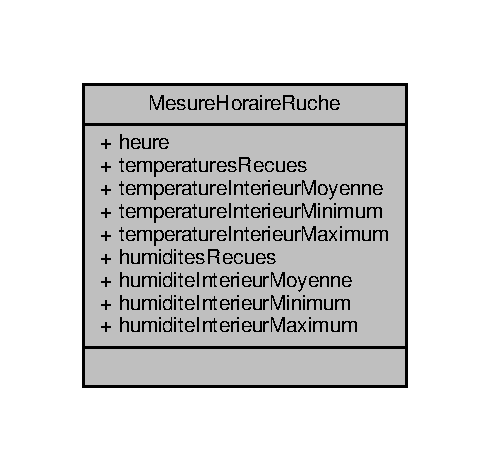
\includegraphics[width=235pt]{struct_mesure_horaire_ruche__coll__graph}
\end{center}
\end{figure}
\subsubsection*{Attributs publics}
\begin{DoxyCompactItemize}
\item 
int \hyperlink{struct_mesure_horaire_ruche_ab679cc7168deb6c3d2458c99b94e0611}{heure}
\item 
bool \hyperlink{struct_mesure_horaire_ruche_ade9984cb0f2c62b3ba1369f77249bb4a}{temperatures\+Recues} = false
\item 
double \hyperlink{struct_mesure_horaire_ruche_ac240bf701116e1a09f2bf33911bf57ef}{temperature\+Interieur\+Moyenne}
\item 
double \hyperlink{struct_mesure_horaire_ruche_a51c45378a78c733704df79b38d61afcc}{temperature\+Interieur\+Minimum}
\item 
double \hyperlink{struct_mesure_horaire_ruche_a746c391a70735bfff63bf7271ab28ab8}{temperature\+Interieur\+Maximum}
\item 
bool \hyperlink{struct_mesure_horaire_ruche_a4f825f05bf4e61db7b18a08dee759b7a}{humidites\+Recues} = false
\item 
double \hyperlink{struct_mesure_horaire_ruche_a46f517d342e230b4e3d0b84a96b79aac}{humidite\+Interieur\+Moyenne}
\item 
double \hyperlink{struct_mesure_horaire_ruche_adf0cbf1a3451cced1ba6fb9573654236}{humidite\+Interieur\+Minimum}
\item 
double \hyperlink{struct_mesure_horaire_ruche_ac8733bd08c235de27dd3eea85749c3f6}{humidite\+Interieur\+Maximum}
\end{DoxyCompactItemize}


\subsubsection{Description détaillée}
\begin{DoxyAuthor}{Auteur}
Florentin Mellah, Enzo Rossi
\end{DoxyAuthor}
\begin{DoxyVersion}{Version}
1.\+1 
\end{DoxyVersion}


\subsubsection{Documentation des données membres}
\mbox{\Hypertarget{struct_mesure_horaire_ruche_ab679cc7168deb6c3d2458c99b94e0611}\label{struct_mesure_horaire_ruche_ab679cc7168deb6c3d2458c99b94e0611}} 
\index{Mesure\+Horaire\+Ruche@{Mesure\+Horaire\+Ruche}!heure@{heure}}
\index{heure@{heure}!Mesure\+Horaire\+Ruche@{Mesure\+Horaire\+Ruche}}
\paragraph{\texorpdfstring{heure}{heure}}
{\footnotesize\ttfamily int Mesure\+Horaire\+Ruche\+::heure}



Référencé par \hyperlink{class_ruche_a3a093c088d9c97f347394c8a681f7302}{Ruche\+::inserer\+Mesure\+Horaire\+Ruche()}, \hyperlink{class_ruche_a6d4c59f2850f803a0ed1946e737b4262}{Ruche\+::recevoir\+Traitement\+Humidite\+Interieur()}, et \hyperlink{class_ruche_a2d2a681916140b977d45423d0d5d7b34}{Ruche\+::recevoir\+Traitement\+Temperature\+Interieur()}.

\mbox{\Hypertarget{struct_mesure_horaire_ruche_ac8733bd08c235de27dd3eea85749c3f6}\label{struct_mesure_horaire_ruche_ac8733bd08c235de27dd3eea85749c3f6}} 
\index{Mesure\+Horaire\+Ruche@{Mesure\+Horaire\+Ruche}!humidite\+Interieur\+Maximum@{humidite\+Interieur\+Maximum}}
\index{humidite\+Interieur\+Maximum@{humidite\+Interieur\+Maximum}!Mesure\+Horaire\+Ruche@{Mesure\+Horaire\+Ruche}}
\paragraph{\texorpdfstring{humidite\+Interieur\+Maximum}{humiditeInterieurMaximum}}
{\footnotesize\ttfamily double Mesure\+Horaire\+Ruche\+::humidite\+Interieur\+Maximum}



Référencé par \hyperlink{class_ruche_a3a093c088d9c97f347394c8a681f7302}{Ruche\+::inserer\+Mesure\+Horaire\+Ruche()}, et \hyperlink{class_ruche_a6d4c59f2850f803a0ed1946e737b4262}{Ruche\+::recevoir\+Traitement\+Humidite\+Interieur()}.

\mbox{\Hypertarget{struct_mesure_horaire_ruche_adf0cbf1a3451cced1ba6fb9573654236}\label{struct_mesure_horaire_ruche_adf0cbf1a3451cced1ba6fb9573654236}} 
\index{Mesure\+Horaire\+Ruche@{Mesure\+Horaire\+Ruche}!humidite\+Interieur\+Minimum@{humidite\+Interieur\+Minimum}}
\index{humidite\+Interieur\+Minimum@{humidite\+Interieur\+Minimum}!Mesure\+Horaire\+Ruche@{Mesure\+Horaire\+Ruche}}
\paragraph{\texorpdfstring{humidite\+Interieur\+Minimum}{humiditeInterieurMinimum}}
{\footnotesize\ttfamily double Mesure\+Horaire\+Ruche\+::humidite\+Interieur\+Minimum}



Référencé par \hyperlink{class_ruche_a3a093c088d9c97f347394c8a681f7302}{Ruche\+::inserer\+Mesure\+Horaire\+Ruche()}, et \hyperlink{class_ruche_a6d4c59f2850f803a0ed1946e737b4262}{Ruche\+::recevoir\+Traitement\+Humidite\+Interieur()}.

\mbox{\Hypertarget{struct_mesure_horaire_ruche_a46f517d342e230b4e3d0b84a96b79aac}\label{struct_mesure_horaire_ruche_a46f517d342e230b4e3d0b84a96b79aac}} 
\index{Mesure\+Horaire\+Ruche@{Mesure\+Horaire\+Ruche}!humidite\+Interieur\+Moyenne@{humidite\+Interieur\+Moyenne}}
\index{humidite\+Interieur\+Moyenne@{humidite\+Interieur\+Moyenne}!Mesure\+Horaire\+Ruche@{Mesure\+Horaire\+Ruche}}
\paragraph{\texorpdfstring{humidite\+Interieur\+Moyenne}{humiditeInterieurMoyenne}}
{\footnotesize\ttfamily double Mesure\+Horaire\+Ruche\+::humidite\+Interieur\+Moyenne}



Référencé par \hyperlink{class_ruche_a3a093c088d9c97f347394c8a681f7302}{Ruche\+::inserer\+Mesure\+Horaire\+Ruche()}, et \hyperlink{class_ruche_a6d4c59f2850f803a0ed1946e737b4262}{Ruche\+::recevoir\+Traitement\+Humidite\+Interieur()}.

\mbox{\Hypertarget{struct_mesure_horaire_ruche_a4f825f05bf4e61db7b18a08dee759b7a}\label{struct_mesure_horaire_ruche_a4f825f05bf4e61db7b18a08dee759b7a}} 
\index{Mesure\+Horaire\+Ruche@{Mesure\+Horaire\+Ruche}!humidites\+Recues@{humidites\+Recues}}
\index{humidites\+Recues@{humidites\+Recues}!Mesure\+Horaire\+Ruche@{Mesure\+Horaire\+Ruche}}
\paragraph{\texorpdfstring{humidites\+Recues}{humiditesRecues}}
{\footnotesize\ttfamily bool Mesure\+Horaire\+Ruche\+::humidites\+Recues = false}



Référencé par \hyperlink{class_ruche_a3a093c088d9c97f347394c8a681f7302}{Ruche\+::inserer\+Mesure\+Horaire\+Ruche()}, et \hyperlink{class_ruche_a6d4c59f2850f803a0ed1946e737b4262}{Ruche\+::recevoir\+Traitement\+Humidite\+Interieur()}.

\mbox{\Hypertarget{struct_mesure_horaire_ruche_a746c391a70735bfff63bf7271ab28ab8}\label{struct_mesure_horaire_ruche_a746c391a70735bfff63bf7271ab28ab8}} 
\index{Mesure\+Horaire\+Ruche@{Mesure\+Horaire\+Ruche}!temperature\+Interieur\+Maximum@{temperature\+Interieur\+Maximum}}
\index{temperature\+Interieur\+Maximum@{temperature\+Interieur\+Maximum}!Mesure\+Horaire\+Ruche@{Mesure\+Horaire\+Ruche}}
\paragraph{\texorpdfstring{temperature\+Interieur\+Maximum}{temperatureInterieurMaximum}}
{\footnotesize\ttfamily double Mesure\+Horaire\+Ruche\+::temperature\+Interieur\+Maximum}



Référencé par \hyperlink{class_ruche_a3a093c088d9c97f347394c8a681f7302}{Ruche\+::inserer\+Mesure\+Horaire\+Ruche()}, et \hyperlink{class_ruche_a2d2a681916140b977d45423d0d5d7b34}{Ruche\+::recevoir\+Traitement\+Temperature\+Interieur()}.

\mbox{\Hypertarget{struct_mesure_horaire_ruche_a51c45378a78c733704df79b38d61afcc}\label{struct_mesure_horaire_ruche_a51c45378a78c733704df79b38d61afcc}} 
\index{Mesure\+Horaire\+Ruche@{Mesure\+Horaire\+Ruche}!temperature\+Interieur\+Minimum@{temperature\+Interieur\+Minimum}}
\index{temperature\+Interieur\+Minimum@{temperature\+Interieur\+Minimum}!Mesure\+Horaire\+Ruche@{Mesure\+Horaire\+Ruche}}
\paragraph{\texorpdfstring{temperature\+Interieur\+Minimum}{temperatureInterieurMinimum}}
{\footnotesize\ttfamily double Mesure\+Horaire\+Ruche\+::temperature\+Interieur\+Minimum}



Référencé par \hyperlink{class_ruche_a3a093c088d9c97f347394c8a681f7302}{Ruche\+::inserer\+Mesure\+Horaire\+Ruche()}, et \hyperlink{class_ruche_a2d2a681916140b977d45423d0d5d7b34}{Ruche\+::recevoir\+Traitement\+Temperature\+Interieur()}.

\mbox{\Hypertarget{struct_mesure_horaire_ruche_ac240bf701116e1a09f2bf33911bf57ef}\label{struct_mesure_horaire_ruche_ac240bf701116e1a09f2bf33911bf57ef}} 
\index{Mesure\+Horaire\+Ruche@{Mesure\+Horaire\+Ruche}!temperature\+Interieur\+Moyenne@{temperature\+Interieur\+Moyenne}}
\index{temperature\+Interieur\+Moyenne@{temperature\+Interieur\+Moyenne}!Mesure\+Horaire\+Ruche@{Mesure\+Horaire\+Ruche}}
\paragraph{\texorpdfstring{temperature\+Interieur\+Moyenne}{temperatureInterieurMoyenne}}
{\footnotesize\ttfamily double Mesure\+Horaire\+Ruche\+::temperature\+Interieur\+Moyenne}



Référencé par \hyperlink{class_ruche_a3a093c088d9c97f347394c8a681f7302}{Ruche\+::inserer\+Mesure\+Horaire\+Ruche()}, et \hyperlink{class_ruche_a2d2a681916140b977d45423d0d5d7b34}{Ruche\+::recevoir\+Traitement\+Temperature\+Interieur()}.

\mbox{\Hypertarget{struct_mesure_horaire_ruche_ade9984cb0f2c62b3ba1369f77249bb4a}\label{struct_mesure_horaire_ruche_ade9984cb0f2c62b3ba1369f77249bb4a}} 
\index{Mesure\+Horaire\+Ruche@{Mesure\+Horaire\+Ruche}!temperatures\+Recues@{temperatures\+Recues}}
\index{temperatures\+Recues@{temperatures\+Recues}!Mesure\+Horaire\+Ruche@{Mesure\+Horaire\+Ruche}}
\paragraph{\texorpdfstring{temperatures\+Recues}{temperaturesRecues}}
{\footnotesize\ttfamily bool Mesure\+Horaire\+Ruche\+::temperatures\+Recues = false}



Référencé par \hyperlink{class_ruche_a3a093c088d9c97f347394c8a681f7302}{Ruche\+::inserer\+Mesure\+Horaire\+Ruche()}, et \hyperlink{class_ruche_a2d2a681916140b977d45423d0d5d7b34}{Ruche\+::recevoir\+Traitement\+Temperature\+Interieur()}.



La documentation de cette structure a été générée à partir du fichier suivant \+:\begin{DoxyCompactItemize}
\item 
\hyperlink{ruche_8h}{ruche.\+h}\end{DoxyCompactItemize}

\hypertarget{struct_mesures_horaire_ensoleillement}{}\subsection{Référence de la structure Mesures\+Horaire\+Ensoleillement}
\label{struct_mesures_horaire_ensoleillement}\index{Mesures\+Horaire\+Ensoleillement@{Mesures\+Horaire\+Ensoleillement}}


structure de données pour les mesures horaires  




{\ttfamily \#include $<$ruche.\+h$>$}



Graphe de collaboration de Mesures\+Horaire\+Ensoleillement\+:\nopagebreak
\begin{figure}[H]
\begin{center}
\leavevmode
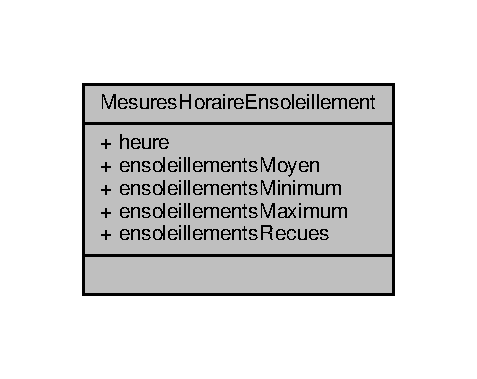
\includegraphics[width=229pt]{struct_mesures_horaire_ensoleillement__coll__graph}
\end{center}
\end{figure}
\subsubsection*{Attributs publics}
\begin{DoxyCompactItemize}
\item 
int \hyperlink{struct_mesures_horaire_ensoleillement_a478cf936fa746f384445cf5077206454}{heure}
\item 
double \hyperlink{struct_mesures_horaire_ensoleillement_a41c11dd16f5e42cf8b4882f98b9cee49}{ensoleillements\+Moyen}
\item 
double \hyperlink{struct_mesures_horaire_ensoleillement_a5d1165f40806663a3fd40ee4408c78f1}{ensoleillements\+Minimum}
\item 
double \hyperlink{struct_mesures_horaire_ensoleillement_adc848a942c5dcb0984b4c346f07e6f09}{ensoleillements\+Maximum}
\item 
bool \hyperlink{struct_mesures_horaire_ensoleillement_a78d40966edb1ace93776ba33edfc5151}{ensoleillements\+Recues} = false
\end{DoxyCompactItemize}


\subsubsection{Description détaillée}
\begin{DoxyAuthor}{Auteur}
Florentin Mellah, Enzo Rossi
\end{DoxyAuthor}
\begin{DoxyVersion}{Version}
1.\+1 
\end{DoxyVersion}


\subsubsection{Documentation des données membres}
\mbox{\Hypertarget{struct_mesures_horaire_ensoleillement_adc848a942c5dcb0984b4c346f07e6f09}\label{struct_mesures_horaire_ensoleillement_adc848a942c5dcb0984b4c346f07e6f09}} 
\index{Mesures\+Horaire\+Ensoleillement@{Mesures\+Horaire\+Ensoleillement}!ensoleillements\+Maximum@{ensoleillements\+Maximum}}
\index{ensoleillements\+Maximum@{ensoleillements\+Maximum}!Mesures\+Horaire\+Ensoleillement@{Mesures\+Horaire\+Ensoleillement}}
\paragraph{\texorpdfstring{ensoleillements\+Maximum}{ensoleillementsMaximum}}
{\footnotesize\ttfamily double Mesures\+Horaire\+Ensoleillement\+::ensoleillements\+Maximum}



Référencé par \hyperlink{class_ruche_a658234b9d96541d204b95b74556742b6}{Ruche\+::inserer\+Mesure\+Horaire\+Ensoleillement()}, et \hyperlink{class_ruche_a2ac5766ce8652084f034c498691488ea}{Ruche\+::recevoir\+Traitement\+Ensoleillement()}.

\mbox{\Hypertarget{struct_mesures_horaire_ensoleillement_a5d1165f40806663a3fd40ee4408c78f1}\label{struct_mesures_horaire_ensoleillement_a5d1165f40806663a3fd40ee4408c78f1}} 
\index{Mesures\+Horaire\+Ensoleillement@{Mesures\+Horaire\+Ensoleillement}!ensoleillements\+Minimum@{ensoleillements\+Minimum}}
\index{ensoleillements\+Minimum@{ensoleillements\+Minimum}!Mesures\+Horaire\+Ensoleillement@{Mesures\+Horaire\+Ensoleillement}}
\paragraph{\texorpdfstring{ensoleillements\+Minimum}{ensoleillementsMinimum}}
{\footnotesize\ttfamily double Mesures\+Horaire\+Ensoleillement\+::ensoleillements\+Minimum}



Référencé par \hyperlink{class_ruche_a658234b9d96541d204b95b74556742b6}{Ruche\+::inserer\+Mesure\+Horaire\+Ensoleillement()}, et \hyperlink{class_ruche_a2ac5766ce8652084f034c498691488ea}{Ruche\+::recevoir\+Traitement\+Ensoleillement()}.

\mbox{\Hypertarget{struct_mesures_horaire_ensoleillement_a41c11dd16f5e42cf8b4882f98b9cee49}\label{struct_mesures_horaire_ensoleillement_a41c11dd16f5e42cf8b4882f98b9cee49}} 
\index{Mesures\+Horaire\+Ensoleillement@{Mesures\+Horaire\+Ensoleillement}!ensoleillements\+Moyen@{ensoleillements\+Moyen}}
\index{ensoleillements\+Moyen@{ensoleillements\+Moyen}!Mesures\+Horaire\+Ensoleillement@{Mesures\+Horaire\+Ensoleillement}}
\paragraph{\texorpdfstring{ensoleillements\+Moyen}{ensoleillementsMoyen}}
{\footnotesize\ttfamily double Mesures\+Horaire\+Ensoleillement\+::ensoleillements\+Moyen}



Référencé par \hyperlink{class_ruche_a658234b9d96541d204b95b74556742b6}{Ruche\+::inserer\+Mesure\+Horaire\+Ensoleillement()}, et \hyperlink{class_ruche_a2ac5766ce8652084f034c498691488ea}{Ruche\+::recevoir\+Traitement\+Ensoleillement()}.

\mbox{\Hypertarget{struct_mesures_horaire_ensoleillement_a78d40966edb1ace93776ba33edfc5151}\label{struct_mesures_horaire_ensoleillement_a78d40966edb1ace93776ba33edfc5151}} 
\index{Mesures\+Horaire\+Ensoleillement@{Mesures\+Horaire\+Ensoleillement}!ensoleillements\+Recues@{ensoleillements\+Recues}}
\index{ensoleillements\+Recues@{ensoleillements\+Recues}!Mesures\+Horaire\+Ensoleillement@{Mesures\+Horaire\+Ensoleillement}}
\paragraph{\texorpdfstring{ensoleillements\+Recues}{ensoleillementsRecues}}
{\footnotesize\ttfamily bool Mesures\+Horaire\+Ensoleillement\+::ensoleillements\+Recues = false}



Référencé par \hyperlink{class_ruche_a658234b9d96541d204b95b74556742b6}{Ruche\+::inserer\+Mesure\+Horaire\+Ensoleillement()}, et \hyperlink{class_ruche_a2ac5766ce8652084f034c498691488ea}{Ruche\+::recevoir\+Traitement\+Ensoleillement()}.

\mbox{\Hypertarget{struct_mesures_horaire_ensoleillement_a478cf936fa746f384445cf5077206454}\label{struct_mesures_horaire_ensoleillement_a478cf936fa746f384445cf5077206454}} 
\index{Mesures\+Horaire\+Ensoleillement@{Mesures\+Horaire\+Ensoleillement}!heure@{heure}}
\index{heure@{heure}!Mesures\+Horaire\+Ensoleillement@{Mesures\+Horaire\+Ensoleillement}}
\paragraph{\texorpdfstring{heure}{heure}}
{\footnotesize\ttfamily int Mesures\+Horaire\+Ensoleillement\+::heure}



Référencé par \hyperlink{class_ruche_a658234b9d96541d204b95b74556742b6}{Ruche\+::inserer\+Mesure\+Horaire\+Ensoleillement()}, et \hyperlink{class_ruche_a2ac5766ce8652084f034c498691488ea}{Ruche\+::recevoir\+Traitement\+Ensoleillement()}.



La documentation de cette structure a été générée à partir du fichier suivant \+:\begin{DoxyCompactItemize}
\item 
\hyperlink{ruche_8h}{ruche.\+h}\end{DoxyCompactItemize}

\hypertarget{classfr_1_1campus_1_1laurainc_1_1honeybee_1_1_nouvelle_ruche_activity}{}\subsection{Référence de la classe fr.\+campus.\+laurainc.\+honeybee.\+Nouvelle\+Ruche\+Activity}
\label{classfr_1_1campus_1_1laurainc_1_1honeybee_1_1_nouvelle_ruche_activity}\index{fr.\+campus.\+laurainc.\+honeybee.\+Nouvelle\+Ruche\+Activity@{fr.\+campus.\+laurainc.\+honeybee.\+Nouvelle\+Ruche\+Activity}}


Graphe de collaboration de fr.\+campus.\+laurainc.\+honeybee.\+Nouvelle\+Ruche\+Activity\+:\nopagebreak
\begin{figure}[H]
\begin{center}
\leavevmode
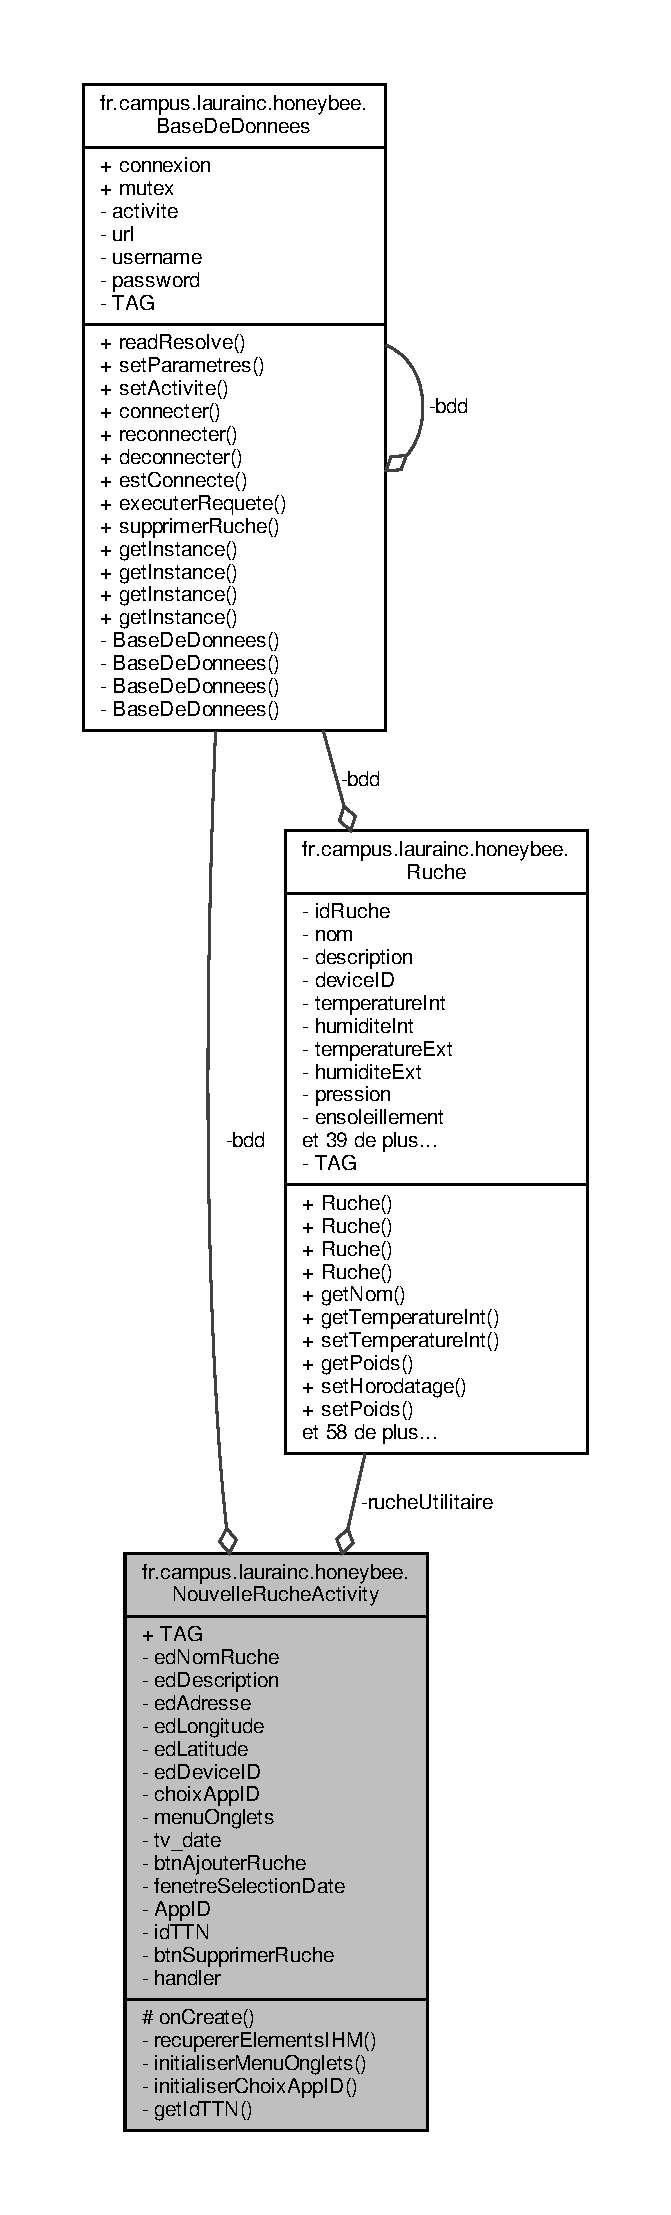
\includegraphics[height=550pt]{classfr_1_1campus_1_1laurainc_1_1honeybee_1_1_nouvelle_ruche_activity__coll__graph}
\end{center}
\end{figure}
\subsubsection*{Attributs publics statiques}
\begin{DoxyCompactItemize}
\item 
static final String \hyperlink{classfr_1_1campus_1_1laurainc_1_1honeybee_1_1_nouvelle_ruche_activity_afa1372bcc0387e18df3877ebe605670d}{T\+AG} = \char`\"{}Nouvelle\+Ruche\+Activity\char`\"{}
\end{DoxyCompactItemize}
\subsubsection*{Fonctions membres protégées}
\begin{DoxyCompactItemize}
\item 
void \hyperlink{classfr_1_1campus_1_1laurainc_1_1honeybee_1_1_nouvelle_ruche_activity_ae97fec78fb0a2e1cc4610182bc71ea0d}{on\+Create} (Bundle saved\+Instance\+State)
\end{DoxyCompactItemize}
\subsubsection*{Fonctions membres privées}
\begin{DoxyCompactItemize}
\item 
void \hyperlink{classfr_1_1campus_1_1laurainc_1_1honeybee_1_1_nouvelle_ruche_activity_adde8644c7ea0259edebc36f15de7a891}{recuperer\+Elements\+I\+HM} ()
\item 
void \hyperlink{classfr_1_1campus_1_1laurainc_1_1honeybee_1_1_nouvelle_ruche_activity_ad9bdfb01df8d7402b4da9858f263e1fd}{initialiser\+Menu\+Onglets} ()
\item 
void \hyperlink{classfr_1_1campus_1_1laurainc_1_1honeybee_1_1_nouvelle_ruche_activity_a25bf91899b217681bda733e7783d0bf9}{initialiser\+Choix\+App\+ID} ()
\item 
void \hyperlink{classfr_1_1campus_1_1laurainc_1_1honeybee_1_1_nouvelle_ruche_activity_a83e03af4d233629129a31cd78f762551}{get\+Id\+T\+TN} ()
\end{DoxyCompactItemize}
\subsubsection*{Attributs privés}
\begin{DoxyCompactItemize}
\item 
Edit\+Text \hyperlink{classfr_1_1campus_1_1laurainc_1_1honeybee_1_1_nouvelle_ruche_activity_aa2d4b480f89c9acf2ddcd4e9677ec406}{ed\+Nom\+Ruche}
\item 
Edit\+Text \hyperlink{classfr_1_1campus_1_1laurainc_1_1honeybee_1_1_nouvelle_ruche_activity_afcd95cec0188630bb413ff73033b9785}{ed\+Description}
\item 
Edit\+Text \hyperlink{classfr_1_1campus_1_1laurainc_1_1honeybee_1_1_nouvelle_ruche_activity_a850ff6dbcd4ee64b7eea6aeebd207d98}{ed\+Adresse}
\item 
Edit\+Text \hyperlink{classfr_1_1campus_1_1laurainc_1_1honeybee_1_1_nouvelle_ruche_activity_aa04d930373ba06878d148bdc001d0e7c}{ed\+Longitude}
\item 
Edit\+Text \hyperlink{classfr_1_1campus_1_1laurainc_1_1honeybee_1_1_nouvelle_ruche_activity_a6673109be623a992ac86b6e5aeed8063}{ed\+Latitude}
\item 
Edit\+Text \hyperlink{classfr_1_1campus_1_1laurainc_1_1honeybee_1_1_nouvelle_ruche_activity_a93bbf506f67bb0b5b3308dc3ba715b9d}{ed\+Device\+ID}
\item 
Spinner \hyperlink{classfr_1_1campus_1_1laurainc_1_1honeybee_1_1_nouvelle_ruche_activity_a9e3885704b27199262c12f0349388009}{choix\+App\+ID}
\item 
Tab\+Host \hyperlink{classfr_1_1campus_1_1laurainc_1_1honeybee_1_1_nouvelle_ruche_activity_a65be1931e07c6e8fb9a2cc5468a2b559}{menu\+Onglets}
\item 
Text\+View \hyperlink{classfr_1_1campus_1_1laurainc_1_1honeybee_1_1_nouvelle_ruche_activity_aaca431bc75d86447e4ecbe01cfa9857d}{tv\+\_\+date}
\item 
Button \hyperlink{classfr_1_1campus_1_1laurainc_1_1honeybee_1_1_nouvelle_ruche_activity_a8f755bb104c7db861c3942ceb56519f4}{btn\+Ajouter\+Ruche}
\item 
Date\+Picker\+Dialog.\+On\+Date\+Set\+Listener \hyperlink{classfr_1_1campus_1_1laurainc_1_1honeybee_1_1_nouvelle_ruche_activity_a41f4797d95ad07979e5a1fc7fb061269}{fenetre\+Selection\+Date}
\item 
\hyperlink{classfr_1_1campus_1_1laurainc_1_1honeybee_1_1_base_de_donnees}{Base\+De\+Donnees} \hyperlink{classfr_1_1campus_1_1laurainc_1_1honeybee_1_1_nouvelle_ruche_activity_ad2073e012bfa9acbe78bac9db9d7d0b4}{bdd} = null
\item 
Array\+List$<$ String $>$ \hyperlink{classfr_1_1campus_1_1laurainc_1_1honeybee_1_1_nouvelle_ruche_activity_a0ff20f2b7c524901d60c78d078999d85}{App\+ID}
\item 
\hyperlink{classfr_1_1campus_1_1laurainc_1_1honeybee_1_1_ruche}{Ruche} \hyperlink{classfr_1_1campus_1_1laurainc_1_1honeybee_1_1_nouvelle_ruche_activity_adad53c25187f84fd37af3d2de167529e}{ruche\+Utilitaire}
\item 
int \hyperlink{classfr_1_1campus_1_1laurainc_1_1honeybee_1_1_nouvelle_ruche_activity_a0e39429b741638b151aec8960b76b0e1}{id\+T\+TN}
\item 
Button \hyperlink{classfr_1_1campus_1_1laurainc_1_1honeybee_1_1_nouvelle_ruche_activity_abd504e41c6cb223e18a106bb1bb62a7d}{btn\+Supprimer\+Ruche}
\item 
final Handler \hyperlink{classfr_1_1campus_1_1laurainc_1_1honeybee_1_1_nouvelle_ruche_activity_a71c7cb93b67cfe6c419c3c6f8504bbc0}{handler}
\end{DoxyCompactItemize}


\subsubsection{Documentation des fonctions membres}
\mbox{\Hypertarget{classfr_1_1campus_1_1laurainc_1_1honeybee_1_1_nouvelle_ruche_activity_a83e03af4d233629129a31cd78f762551}\label{classfr_1_1campus_1_1laurainc_1_1honeybee_1_1_nouvelle_ruche_activity_a83e03af4d233629129a31cd78f762551}} 
\index{fr\+::campus\+::laurainc\+::honeybee\+::\+Nouvelle\+Ruche\+Activity@{fr\+::campus\+::laurainc\+::honeybee\+::\+Nouvelle\+Ruche\+Activity}!get\+Id\+T\+TN@{get\+Id\+T\+TN}}
\index{get\+Id\+T\+TN@{get\+Id\+T\+TN}!fr\+::campus\+::laurainc\+::honeybee\+::\+Nouvelle\+Ruche\+Activity@{fr\+::campus\+::laurainc\+::honeybee\+::\+Nouvelle\+Ruche\+Activity}}
\paragraph{\texorpdfstring{get\+Id\+T\+T\+N()}{getIdTTN()}}
{\footnotesize\ttfamily void fr.\+campus.\+laurainc.\+honeybee.\+Nouvelle\+Ruche\+Activity.\+get\+Id\+T\+TN (\begin{DoxyParamCaption}{ }\end{DoxyParamCaption})\hspace{0.3cm}{\ttfamily [private]}}



Références \hyperlink{classfr_1_1campus_1_1laurainc_1_1honeybee_1_1_ruche_a8c4c0db39c42733517035c4211e0ff95}{fr.\+campus.\+laurainc.\+honeybee.\+Ruche.\+get\+Id\+T\+T\+N\+Selectionne()}.


\begin{DoxyCode}
00147     \{
00148         \hyperlink{classfr_1_1campus_1_1laurainc_1_1honeybee_1_1_nouvelle_ruche_activity_a0e39429b741638b151aec8960b76b0e1}{idTTN} = \hyperlink{classfr_1_1campus_1_1laurainc_1_1honeybee_1_1_nouvelle_ruche_activity_adad53c25187f84fd37af3d2de167529e}{rucheUtilitaire}.\hyperlink{classfr_1_1campus_1_1laurainc_1_1honeybee_1_1_ruche_a8c4c0db39c42733517035c4211e0ff95}{getIdTTNSelectionne}();
00149         Log.d(\hyperlink{classfr_1_1campus_1_1laurainc_1_1honeybee_1_1_nouvelle_ruche_activity_afa1372bcc0387e18df3877ebe605670d}{TAG}, \textcolor{stringliteral}{"IdTTN :"} + \hyperlink{classfr_1_1campus_1_1laurainc_1_1honeybee_1_1_nouvelle_ruche_activity_a0e39429b741638b151aec8960b76b0e1}{idTTN});
00150     \}
\end{DoxyCode}
\mbox{\Hypertarget{classfr_1_1campus_1_1laurainc_1_1honeybee_1_1_nouvelle_ruche_activity_a25bf91899b217681bda733e7783d0bf9}\label{classfr_1_1campus_1_1laurainc_1_1honeybee_1_1_nouvelle_ruche_activity_a25bf91899b217681bda733e7783d0bf9}} 
\index{fr\+::campus\+::laurainc\+::honeybee\+::\+Nouvelle\+Ruche\+Activity@{fr\+::campus\+::laurainc\+::honeybee\+::\+Nouvelle\+Ruche\+Activity}!initialiser\+Choix\+App\+ID@{initialiser\+Choix\+App\+ID}}
\index{initialiser\+Choix\+App\+ID@{initialiser\+Choix\+App\+ID}!fr\+::campus\+::laurainc\+::honeybee\+::\+Nouvelle\+Ruche\+Activity@{fr\+::campus\+::laurainc\+::honeybee\+::\+Nouvelle\+Ruche\+Activity}}
\paragraph{\texorpdfstring{initialiser\+Choix\+App\+I\+D()}{initialiserChoixAppID()}}
{\footnotesize\ttfamily void fr.\+campus.\+laurainc.\+honeybee.\+Nouvelle\+Ruche\+Activity.\+initialiser\+Choix\+App\+ID (\begin{DoxyParamCaption}{ }\end{DoxyParamCaption})\hspace{0.3cm}{\ttfamily [private]}}



Références \hyperlink{classfr_1_1campus_1_1laurainc_1_1honeybee_1_1_nouvelle_ruche_activity_a0ff20f2b7c524901d60c78d078999d85}{fr.\+campus.\+laurainc.\+honeybee.\+Nouvelle\+Ruche\+Activity.\+App\+ID}, \hyperlink{classfr_1_1campus_1_1laurainc_1_1honeybee_1_1_ruche_a08d58dc3ce2db9adc37903c9b2f08977}{fr.\+campus.\+laurainc.\+honeybee.\+Ruche.\+get\+Liste\+Choix\+App\+I\+D()}, et \hyperlink{classfr_1_1campus_1_1laurainc_1_1honeybee_1_1_ruche_a1113f3b4a527a801fdf50350667fd212}{fr.\+campus.\+laurainc.\+honeybee.\+Ruche.\+recuperer\+Id\+T\+T\+N()}.


\begin{DoxyCode}
00121                                          \{
00122         \hyperlink{classfr_1_1campus_1_1laurainc_1_1honeybee_1_1_nouvelle_ruche_activity_a0ff20f2b7c524901d60c78d078999d85}{AppID} = \hyperlink{classfr_1_1campus_1_1laurainc_1_1honeybee_1_1_nouvelle_ruche_activity_adad53c25187f84fd37af3d2de167529e}{rucheUtilitaire}.\hyperlink{classfr_1_1campus_1_1laurainc_1_1honeybee_1_1_ruche_a08d58dc3ce2db9adc37903c9b2f08977}{getListeChoixAppID}();
00123         ArrayAdapter<String> adapter = \textcolor{keyword}{new} ArrayAdapter<String>(\textcolor{keyword}{this}, android.R.layout.simple\_spinner\_item,
       \hyperlink{classfr_1_1campus_1_1laurainc_1_1honeybee_1_1_nouvelle_ruche_activity_a0ff20f2b7c524901d60c78d078999d85}{AppID});
00124         adapter.setDropDownViewResource(android.R.layout.simple\_spinner\_dropdown\_item);
00125         \hyperlink{classfr_1_1campus_1_1laurainc_1_1honeybee_1_1_nouvelle_ruche_activity_a9e3885704b27199262c12f0349388009}{choixAppID}.setAdapter(adapter);
00126         \hyperlink{classfr_1_1campus_1_1laurainc_1_1honeybee_1_1_nouvelle_ruche_activity_a9e3885704b27199262c12f0349388009}{choixAppID}.setSelection(0);
00127 
00128         \hyperlink{classfr_1_1campus_1_1laurainc_1_1honeybee_1_1_nouvelle_ruche_activity_a9e3885704b27199262c12f0349388009}{choixAppID}.setOnItemSelectedListener(\textcolor{keyword}{new} AdapterView.OnItemSelectedListener()
00129         \{
00130             @Override
00131             \textcolor{keyword}{public} \textcolor{keywordtype}{void} onItemSelected(AdapterView<?> arg0, View arg1, \textcolor{keywordtype}{int} position, \textcolor{keywordtype}{long} \textcolor{keywordtype}{id})
00132             \{
00133                 Log.d(\hyperlink{classfr_1_1campus_1_1laurainc_1_1honeybee_1_1_nouvelle_ruche_activity_afa1372bcc0387e18df3877ebe605670d}{TAG}, \textcolor{stringliteral}{"position : "} + position);
00134                 Log.d(\hyperlink{classfr_1_1campus_1_1laurainc_1_1honeybee_1_1_nouvelle_ruche_activity_afa1372bcc0387e18df3877ebe605670d}{TAG}, \textcolor{stringliteral}{"AppID Sélectionné : "} + \hyperlink{classfr_1_1campus_1_1laurainc_1_1honeybee_1_1_nouvelle_ruche_activity_a0ff20f2b7c524901d60c78d078999d85}{AppID}.get(position));
00135                 \hyperlink{classfr_1_1campus_1_1laurainc_1_1honeybee_1_1_nouvelle_ruche_activity_adad53c25187f84fd37af3d2de167529e}{rucheUtilitaire}.\hyperlink{classfr_1_1campus_1_1laurainc_1_1honeybee_1_1_ruche_a1113f3b4a527a801fdf50350667fd212}{recupererIdTTN}(
      \hyperlink{classfr_1_1campus_1_1laurainc_1_1honeybee_1_1_nouvelle_ruche_activity_a0ff20f2b7c524901d60c78d078999d85}{AppID}.get(position));
00136             \}
00137 
00138             @Override
00139             \textcolor{keyword}{public} \textcolor{keywordtype}{void} onNothingSelected(AdapterView<?> arg0)
00140             \{
00141                 \textcolor{comment}{// TODO Auto-generated method stub}
00142             \}
00143         \});
00144     \}
\end{DoxyCode}
\mbox{\Hypertarget{classfr_1_1campus_1_1laurainc_1_1honeybee_1_1_nouvelle_ruche_activity_ad9bdfb01df8d7402b4da9858f263e1fd}\label{classfr_1_1campus_1_1laurainc_1_1honeybee_1_1_nouvelle_ruche_activity_ad9bdfb01df8d7402b4da9858f263e1fd}} 
\index{fr\+::campus\+::laurainc\+::honeybee\+::\+Nouvelle\+Ruche\+Activity@{fr\+::campus\+::laurainc\+::honeybee\+::\+Nouvelle\+Ruche\+Activity}!initialiser\+Menu\+Onglets@{initialiser\+Menu\+Onglets}}
\index{initialiser\+Menu\+Onglets@{initialiser\+Menu\+Onglets}!fr\+::campus\+::laurainc\+::honeybee\+::\+Nouvelle\+Ruche\+Activity@{fr\+::campus\+::laurainc\+::honeybee\+::\+Nouvelle\+Ruche\+Activity}}
\paragraph{\texorpdfstring{initialiser\+Menu\+Onglets()}{initialiserMenuOnglets()}}
{\footnotesize\ttfamily void fr.\+campus.\+laurainc.\+honeybee.\+Nouvelle\+Ruche\+Activity.\+initialiser\+Menu\+Onglets (\begin{DoxyParamCaption}{ }\end{DoxyParamCaption})\hspace{0.3cm}{\ttfamily [private]}}



Références \hyperlink{classfr_1_1campus_1_1laurainc_1_1honeybee_1_1_nouvelle_ruche_activity_a71c7cb93b67cfe6c419c3c6f8504bbc0}{fr.\+campus.\+laurainc.\+honeybee.\+Nouvelle\+Ruche\+Activity.\+handler}, et \hyperlink{classfr_1_1campus_1_1laurainc_1_1honeybee_1_1_ruche_ade5d681bd0a29d84e0d069169b10a38b}{fr.\+campus.\+laurainc.\+honeybee.\+Ruche.\+recuperer\+Choix\+Ch\+App\+I\+D()}.



Référencé par \hyperlink{classfr_1_1campus_1_1laurainc_1_1honeybee_1_1_nouvelle_ruche_activity_ae97fec78fb0a2e1cc4610182bc71ea0d}{fr.\+campus.\+laurainc.\+honeybee.\+Nouvelle\+Ruche\+Activity.\+on\+Create()}.


\begin{DoxyCode}
00114     \{
00115         \hyperlink{classfr_1_1campus_1_1laurainc_1_1honeybee_1_1_nouvelle_ruche_activity_adad53c25187f84fd37af3d2de167529e}{rucheUtilitaire} = \textcolor{keyword}{new} \hyperlink{class_ruche}{Ruche}(\hyperlink{classfr_1_1campus_1_1laurainc_1_1honeybee_1_1_nouvelle_ruche_activity_a71c7cb93b67cfe6c419c3c6f8504bbc0}{handler});
00116         Log.d(\hyperlink{classfr_1_1campus_1_1laurainc_1_1honeybee_1_1_nouvelle_ruche_activity_afa1372bcc0387e18df3877ebe605670d}{TAG}, \textcolor{stringliteral}{"Ruche utilitaire créée"});
00117         \hyperlink{classfr_1_1campus_1_1laurainc_1_1honeybee_1_1_nouvelle_ruche_activity_adad53c25187f84fd37af3d2de167529e}{rucheUtilitaire}.\hyperlink{classfr_1_1campus_1_1laurainc_1_1honeybee_1_1_ruche_ade5d681bd0a29d84e0d069169b10a38b}{recupererChoixChAppID}();
00118         Log.d(\hyperlink{classfr_1_1campus_1_1laurainc_1_1honeybee_1_1_nouvelle_ruche_activity_afa1372bcc0387e18df3877ebe605670d}{TAG}, \textcolor{stringliteral}{"Recuperation de la liste des App ID"});
00119     \}
\end{DoxyCode}
\mbox{\Hypertarget{classfr_1_1campus_1_1laurainc_1_1honeybee_1_1_nouvelle_ruche_activity_ae97fec78fb0a2e1cc4610182bc71ea0d}\label{classfr_1_1campus_1_1laurainc_1_1honeybee_1_1_nouvelle_ruche_activity_ae97fec78fb0a2e1cc4610182bc71ea0d}} 
\index{fr\+::campus\+::laurainc\+::honeybee\+::\+Nouvelle\+Ruche\+Activity@{fr\+::campus\+::laurainc\+::honeybee\+::\+Nouvelle\+Ruche\+Activity}!on\+Create@{on\+Create}}
\index{on\+Create@{on\+Create}!fr\+::campus\+::laurainc\+::honeybee\+::\+Nouvelle\+Ruche\+Activity@{fr\+::campus\+::laurainc\+::honeybee\+::\+Nouvelle\+Ruche\+Activity}}
\paragraph{\texorpdfstring{on\+Create()}{onCreate()}}
{\footnotesize\ttfamily void fr.\+campus.\+laurainc.\+honeybee.\+Nouvelle\+Ruche\+Activity.\+on\+Create (\begin{DoxyParamCaption}\item[{Bundle}]{saved\+Instance\+State }\end{DoxyParamCaption})\hspace{0.3cm}{\ttfamily [protected]}}



Références \hyperlink{classfr_1_1campus_1_1laurainc_1_1honeybee_1_1_honey_bee_abfb4f6cc1c8bb793c37ccb8408abc51c}{fr.\+campus.\+laurainc.\+honeybee.\+Honey\+Bee.\+B\+DD}, \hyperlink{classfr_1_1campus_1_1laurainc_1_1honeybee_1_1_base_de_donnees_a08564ea7dccde161d6eac4b8879401bb}{fr.\+campus.\+laurainc.\+honeybee.\+Base\+De\+Donnees.\+connecter()}, \hyperlink{classfr_1_1campus_1_1laurainc_1_1honeybee_1_1_base_de_donnees_a421bffe6f14c01bee64695e7b6a9745d}{fr.\+campus.\+laurainc.\+honeybee.\+Base\+De\+Donnees.\+executer\+Requete()}, \hyperlink{classfr_1_1campus_1_1laurainc_1_1honeybee_1_1_nouvelle_ruche_activity_a41f4797d95ad07979e5a1fc7fb061269}{fr.\+campus.\+laurainc.\+honeybee.\+Nouvelle\+Ruche\+Activity.\+fenetre\+Selection\+Date}, \hyperlink{classfr_1_1campus_1_1laurainc_1_1honeybee_1_1_base_de_donnees_a9c2484cfb87f90e46cf878eb7803abb2}{fr.\+campus.\+laurainc.\+honeybee.\+Base\+De\+Donnees.\+get\+Instance()}, \hyperlink{classfr_1_1campus_1_1laurainc_1_1honeybee_1_1_nouvelle_ruche_activity_ad9bdfb01df8d7402b4da9858f263e1fd}{fr.\+campus.\+laurainc.\+honeybee.\+Nouvelle\+Ruche\+Activity.\+initialiser\+Menu\+Onglets()}, et \hyperlink{classfr_1_1campus_1_1laurainc_1_1honeybee_1_1_nouvelle_ruche_activity_adde8644c7ea0259edebc36f15de7a891}{fr.\+campus.\+laurainc.\+honeybee.\+Nouvelle\+Ruche\+Activity.\+recuperer\+Elements\+I\+H\+M()}.


\begin{DoxyCode}
00050                                                        \{
00051         super.onCreate(savedInstanceState);
00052         setContentView(R.layout.activity\_nouvelle\_ruche);
00053 
00054         \hyperlink{classfr_1_1campus_1_1laurainc_1_1honeybee_1_1_nouvelle_ruche_activity_adde8644c7ea0259edebc36f15de7a891}{recupererElementsIHM}();
00055         \hyperlink{classfr_1_1campus_1_1laurainc_1_1honeybee_1_1_nouvelle_ruche_activity_ad9bdfb01df8d7402b4da9858f263e1fd}{initialiserMenuOnglets}();
00056 
00057        \hyperlink{classfr_1_1campus_1_1laurainc_1_1honeybee_1_1_nouvelle_ruche_activity_aaca431bc75d86447e4ecbe01cfa9857d}{tv\_date}.setOnClickListener(\textcolor{keyword}{new} View.OnClickListener() \{
00058            @Override
00059            \textcolor{keyword}{public} \textcolor{keywordtype}{void} onClick(View v) \{
00060                Calendar calendrier = Calendar.getInstance();
00061                \textcolor{keywordtype}{int} annee = calendrier.get(Calendar.YEAR);
00062                \textcolor{keywordtype}{int} mois = calendrier.get(Calendar.MONTH);
00063                \textcolor{keywordtype}{int} jour = calendrier.get(Calendar.DAY\_OF\_MONTH);
00064 
00065                DatePickerDialog dialog = \textcolor{keyword}{new} DatePickerDialog(NouvelleRucheActivity.this, android.R.style.
      Theme\_DeviceDefault\_Light\_Dialog, \hyperlink{classfr_1_1campus_1_1laurainc_1_1honeybee_1_1_nouvelle_ruche_activity_a41f4797d95ad07979e5a1fc7fb061269}{fenetreSelectionDate}, annee, mois, jour);
00066 
00067                dialog.getWindow().setBackgroundDrawable(\textcolor{keyword}{new} ColorDrawable(Color.WHITE));
00068                dialog.show();
00069            \}
00070        \});
00071 
00072        \hyperlink{classfr_1_1campus_1_1laurainc_1_1honeybee_1_1_nouvelle_ruche_activity_a41f4797d95ad07979e5a1fc7fb061269}{fenetreSelectionDate} = \textcolor{keyword}{new} DatePickerDialog.OnDateSetListener() \{
00073            @Override
00074            \textcolor{keyword}{public} \textcolor{keywordtype}{void} onDateSet(DatePicker view, \textcolor{keywordtype}{int} year, \textcolor{keywordtype}{int} month, \textcolor{keywordtype}{int} dayOfMonth) \{
00075                month = month +1;
00076                Log.d(\hyperlink{classfr_1_1campus_1_1laurainc_1_1honeybee_1_1_nouvelle_ruche_activity_afa1372bcc0387e18df3877ebe605670d}{TAG}, \textcolor{stringliteral}{"Date sélectionnée "} + dayOfMonth + \textcolor{stringliteral}{"/"} + month + \textcolor{stringliteral}{"/"} + year );
00077 
00078                String date = year + \textcolor{stringliteral}{"-"} + month + \textcolor{stringliteral}{"-"} + dayOfMonth;
00079                \hyperlink{classfr_1_1campus_1_1laurainc_1_1honeybee_1_1_nouvelle_ruche_activity_aaca431bc75d86447e4ecbe01cfa9857d}{tv\_date}.setText(date);
00080 
00081            \}
00082        \};
00083 
00084        \hyperlink{classfr_1_1campus_1_1laurainc_1_1honeybee_1_1_nouvelle_ruche_activity_a8f755bb104c7db861c3942ceb56519f4}{btnAjouterRuche}.setOnClickListener(\textcolor{keyword}{new} View.OnClickListener() \{
00085            @Override
00086            \textcolor{keyword}{public} \textcolor{keywordtype}{void} onClick(View v) \{
00087                \textcolor{keywordflow}{if} (HoneyBee.BDD) \{
00088                    \hyperlink{classfr_1_1campus_1_1laurainc_1_1honeybee_1_1_nouvelle_ruche_activity_ad2073e012bfa9acbe78bac9db9d7d0b4}{bdd} = \hyperlink{class_base_de_donnees}{BaseDeDonnees}.\hyperlink{class_base_de_donnees_a80028aa2b6b4fbf30fb2e36357b7d3d3}{getInstance}();
00089                    \hyperlink{classfr_1_1campus_1_1laurainc_1_1honeybee_1_1_nouvelle_ruche_activity_ad2073e012bfa9acbe78bac9db9d7d0b4}{bdd}.\hyperlink{classfr_1_1campus_1_1laurainc_1_1honeybee_1_1_base_de_donnees_a08564ea7dccde161d6eac4b8879401bb}{connecter}();
00090                    \hyperlink{classfr_1_1campus_1_1laurainc_1_1honeybee_1_1_nouvelle_ruche_activity_ad2073e012bfa9acbe78bac9db9d7d0b4}{bdd}.\hyperlink{classfr_1_1campus_1_1laurainc_1_1honeybee_1_1_base_de_donnees_a421bffe6f14c01bee64695e7b6a9745d}{executerRequete}(\textcolor{stringliteral}{"INSERT INTO Ruche (idTTN, Nom, Description,
       DateMiseEnService, Adresse, Longitude, Latitude, DeviceID) VALUES('"}+ \hyperlink{classfr_1_1campus_1_1laurainc_1_1honeybee_1_1_nouvelle_ruche_activity_a0e39429b741638b151aec8960b76b0e1}{idTTN} + \textcolor{stringliteral}{"', '"} + 
      \hyperlink{classfr_1_1campus_1_1laurainc_1_1honeybee_1_1_nouvelle_ruche_activity_aa2d4b480f89c9acf2ddcd4e9677ec406}{edNomRuche}.getText() + \textcolor{stringliteral}{"','"} + \hyperlink{classfr_1_1campus_1_1laurainc_1_1honeybee_1_1_nouvelle_ruche_activity_afcd95cec0188630bb413ff73033b9785}{edDescription}.getText() + \textcolor{stringliteral}{"','"} + 
      \hyperlink{classfr_1_1campus_1_1laurainc_1_1honeybee_1_1_nouvelle_ruche_activity_aaca431bc75d86447e4ecbe01cfa9857d}{tv\_date}.getText() + \textcolor{stringliteral}{"','"} + \hyperlink{classfr_1_1campus_1_1laurainc_1_1honeybee_1_1_nouvelle_ruche_activity_a850ff6dbcd4ee64b7eea6aeebd207d98}{edAdresse}.getText() + \textcolor{stringliteral}{"','"} + 
      \hyperlink{classfr_1_1campus_1_1laurainc_1_1honeybee_1_1_nouvelle_ruche_activity_aa04d930373ba06878d148bdc001d0e7c}{edLongitude}.getText() + \textcolor{stringliteral}{"','"} + \hyperlink{classfr_1_1campus_1_1laurainc_1_1honeybee_1_1_nouvelle_ruche_activity_a6673109be623a992ac86b6e5aeed8063}{edLatitude}.getText() + \textcolor{stringliteral}{"','"} + 
      \hyperlink{classfr_1_1campus_1_1laurainc_1_1honeybee_1_1_nouvelle_ruche_activity_a93bbf506f67bb0b5b3308dc3ba715b9d}{edDeviceID}.getText() + \textcolor{stringliteral}{"')"});
00091                    \textcolor{keyword}{final} Intent nouvelleRuche = \textcolor{keyword}{new} Intent(NouvelleRucheActivity.this, DashboardActivity.
      class);
00092                    startActivity(nouvelleRuche);
00093                \}
00094            \}
00095        \});
00096 
00097     \}
\end{DoxyCode}
\mbox{\Hypertarget{classfr_1_1campus_1_1laurainc_1_1honeybee_1_1_nouvelle_ruche_activity_adde8644c7ea0259edebc36f15de7a891}\label{classfr_1_1campus_1_1laurainc_1_1honeybee_1_1_nouvelle_ruche_activity_adde8644c7ea0259edebc36f15de7a891}} 
\index{fr\+::campus\+::laurainc\+::honeybee\+::\+Nouvelle\+Ruche\+Activity@{fr\+::campus\+::laurainc\+::honeybee\+::\+Nouvelle\+Ruche\+Activity}!recuperer\+Elements\+I\+HM@{recuperer\+Elements\+I\+HM}}
\index{recuperer\+Elements\+I\+HM@{recuperer\+Elements\+I\+HM}!fr\+::campus\+::laurainc\+::honeybee\+::\+Nouvelle\+Ruche\+Activity@{fr\+::campus\+::laurainc\+::honeybee\+::\+Nouvelle\+Ruche\+Activity}}
\paragraph{\texorpdfstring{recuperer\+Elements\+I\+H\+M()}{recupererElementsIHM()}}
{\footnotesize\ttfamily void fr.\+campus.\+laurainc.\+honeybee.\+Nouvelle\+Ruche\+Activity.\+recuperer\+Elements\+I\+HM (\begin{DoxyParamCaption}{ }\end{DoxyParamCaption})\hspace{0.3cm}{\ttfamily [private]}}



Référencé par \hyperlink{classfr_1_1campus_1_1laurainc_1_1honeybee_1_1_nouvelle_ruche_activity_ae97fec78fb0a2e1cc4610182bc71ea0d}{fr.\+campus.\+laurainc.\+honeybee.\+Nouvelle\+Ruche\+Activity.\+on\+Create()}.


\begin{DoxyCode}
00100     \{
00101         \hyperlink{classfr_1_1campus_1_1laurainc_1_1honeybee_1_1_nouvelle_ruche_activity_aa2d4b480f89c9acf2ddcd4e9677ec406}{edNomRuche} = (EditText) findViewById(R.id.edNomRuche);
00102         \hyperlink{classfr_1_1campus_1_1laurainc_1_1honeybee_1_1_nouvelle_ruche_activity_afcd95cec0188630bb413ff73033b9785}{edDescription} = (EditText) findViewById(R.id.edDesciption);
00103         \hyperlink{classfr_1_1campus_1_1laurainc_1_1honeybee_1_1_nouvelle_ruche_activity_a850ff6dbcd4ee64b7eea6aeebd207d98}{edAdresse} = (EditText) findViewById(R.id.edAdresseRuche);
00104         \hyperlink{classfr_1_1campus_1_1laurainc_1_1honeybee_1_1_nouvelle_ruche_activity_aa04d930373ba06878d148bdc001d0e7c}{edLongitude} = (EditText) findViewById(R.id.edLongitude);
00105         \hyperlink{classfr_1_1campus_1_1laurainc_1_1honeybee_1_1_nouvelle_ruche_activity_a6673109be623a992ac86b6e5aeed8063}{edLatitude} = (EditText) findViewById(R.id.edLatitude);
00106         \hyperlink{classfr_1_1campus_1_1laurainc_1_1honeybee_1_1_nouvelle_ruche_activity_a93bbf506f67bb0b5b3308dc3ba715b9d}{edDeviceID} = (EditText) findViewById(R.id.edDeviceID);
00107         \hyperlink{classfr_1_1campus_1_1laurainc_1_1honeybee_1_1_nouvelle_ruche_activity_aaca431bc75d86447e4ecbe01cfa9857d}{tv\_date} = (TextView) findViewById(R.id.tv\_date);
00108         \hyperlink{classfr_1_1campus_1_1laurainc_1_1honeybee_1_1_nouvelle_ruche_activity_a8f755bb104c7db861c3942ceb56519f4}{btnAjouterRuche} = (Button) findViewById(R.id.btnAjouterRuche);
00109         \hyperlink{classfr_1_1campus_1_1laurainc_1_1honeybee_1_1_nouvelle_ruche_activity_a9e3885704b27199262c12f0349388009}{choixAppID} = (Spinner) findViewById(R.id.spinner\_AppID);
00110 
00111     \}
\end{DoxyCode}


\subsubsection{Documentation des données membres}
\mbox{\Hypertarget{classfr_1_1campus_1_1laurainc_1_1honeybee_1_1_nouvelle_ruche_activity_a0ff20f2b7c524901d60c78d078999d85}\label{classfr_1_1campus_1_1laurainc_1_1honeybee_1_1_nouvelle_ruche_activity_a0ff20f2b7c524901d60c78d078999d85}} 
\index{fr\+::campus\+::laurainc\+::honeybee\+::\+Nouvelle\+Ruche\+Activity@{fr\+::campus\+::laurainc\+::honeybee\+::\+Nouvelle\+Ruche\+Activity}!App\+ID@{App\+ID}}
\index{App\+ID@{App\+ID}!fr\+::campus\+::laurainc\+::honeybee\+::\+Nouvelle\+Ruche\+Activity@{fr\+::campus\+::laurainc\+::honeybee\+::\+Nouvelle\+Ruche\+Activity}}
\paragraph{\texorpdfstring{App\+ID}{AppID}}
{\footnotesize\ttfamily Array\+List$<$String$>$ fr.\+campus.\+laurainc.\+honeybee.\+Nouvelle\+Ruche\+Activity.\+App\+ID\hspace{0.3cm}{\ttfamily [private]}}



Référencé par \hyperlink{classfr_1_1campus_1_1laurainc_1_1honeybee_1_1_nouvelle_ruche_activity_a25bf91899b217681bda733e7783d0bf9}{fr.\+campus.\+laurainc.\+honeybee.\+Nouvelle\+Ruche\+Activity.\+initialiser\+Choix\+App\+I\+D()}.

\mbox{\Hypertarget{classfr_1_1campus_1_1laurainc_1_1honeybee_1_1_nouvelle_ruche_activity_ad2073e012bfa9acbe78bac9db9d7d0b4}\label{classfr_1_1campus_1_1laurainc_1_1honeybee_1_1_nouvelle_ruche_activity_ad2073e012bfa9acbe78bac9db9d7d0b4}} 
\index{fr\+::campus\+::laurainc\+::honeybee\+::\+Nouvelle\+Ruche\+Activity@{fr\+::campus\+::laurainc\+::honeybee\+::\+Nouvelle\+Ruche\+Activity}!bdd@{bdd}}
\index{bdd@{bdd}!fr\+::campus\+::laurainc\+::honeybee\+::\+Nouvelle\+Ruche\+Activity@{fr\+::campus\+::laurainc\+::honeybee\+::\+Nouvelle\+Ruche\+Activity}}
\paragraph{\texorpdfstring{bdd}{bdd}}
{\footnotesize\ttfamily \hyperlink{classfr_1_1campus_1_1laurainc_1_1honeybee_1_1_base_de_donnees}{Base\+De\+Donnees} fr.\+campus.\+laurainc.\+honeybee.\+Nouvelle\+Ruche\+Activity.\+bdd = null\hspace{0.3cm}{\ttfamily [private]}}

\mbox{\Hypertarget{classfr_1_1campus_1_1laurainc_1_1honeybee_1_1_nouvelle_ruche_activity_a8f755bb104c7db861c3942ceb56519f4}\label{classfr_1_1campus_1_1laurainc_1_1honeybee_1_1_nouvelle_ruche_activity_a8f755bb104c7db861c3942ceb56519f4}} 
\index{fr\+::campus\+::laurainc\+::honeybee\+::\+Nouvelle\+Ruche\+Activity@{fr\+::campus\+::laurainc\+::honeybee\+::\+Nouvelle\+Ruche\+Activity}!btn\+Ajouter\+Ruche@{btn\+Ajouter\+Ruche}}
\index{btn\+Ajouter\+Ruche@{btn\+Ajouter\+Ruche}!fr\+::campus\+::laurainc\+::honeybee\+::\+Nouvelle\+Ruche\+Activity@{fr\+::campus\+::laurainc\+::honeybee\+::\+Nouvelle\+Ruche\+Activity}}
\paragraph{\texorpdfstring{btn\+Ajouter\+Ruche}{btnAjouterRuche}}
{\footnotesize\ttfamily Button fr.\+campus.\+laurainc.\+honeybee.\+Nouvelle\+Ruche\+Activity.\+btn\+Ajouter\+Ruche\hspace{0.3cm}{\ttfamily [private]}}

\mbox{\Hypertarget{classfr_1_1campus_1_1laurainc_1_1honeybee_1_1_nouvelle_ruche_activity_abd504e41c6cb223e18a106bb1bb62a7d}\label{classfr_1_1campus_1_1laurainc_1_1honeybee_1_1_nouvelle_ruche_activity_abd504e41c6cb223e18a106bb1bb62a7d}} 
\index{fr\+::campus\+::laurainc\+::honeybee\+::\+Nouvelle\+Ruche\+Activity@{fr\+::campus\+::laurainc\+::honeybee\+::\+Nouvelle\+Ruche\+Activity}!btn\+Supprimer\+Ruche@{btn\+Supprimer\+Ruche}}
\index{btn\+Supprimer\+Ruche@{btn\+Supprimer\+Ruche}!fr\+::campus\+::laurainc\+::honeybee\+::\+Nouvelle\+Ruche\+Activity@{fr\+::campus\+::laurainc\+::honeybee\+::\+Nouvelle\+Ruche\+Activity}}
\paragraph{\texorpdfstring{btn\+Supprimer\+Ruche}{btnSupprimerRuche}}
{\footnotesize\ttfamily Button fr.\+campus.\+laurainc.\+honeybee.\+Nouvelle\+Ruche\+Activity.\+btn\+Supprimer\+Ruche\hspace{0.3cm}{\ttfamily [private]}}

\mbox{\Hypertarget{classfr_1_1campus_1_1laurainc_1_1honeybee_1_1_nouvelle_ruche_activity_a9e3885704b27199262c12f0349388009}\label{classfr_1_1campus_1_1laurainc_1_1honeybee_1_1_nouvelle_ruche_activity_a9e3885704b27199262c12f0349388009}} 
\index{fr\+::campus\+::laurainc\+::honeybee\+::\+Nouvelle\+Ruche\+Activity@{fr\+::campus\+::laurainc\+::honeybee\+::\+Nouvelle\+Ruche\+Activity}!choix\+App\+ID@{choix\+App\+ID}}
\index{choix\+App\+ID@{choix\+App\+ID}!fr\+::campus\+::laurainc\+::honeybee\+::\+Nouvelle\+Ruche\+Activity@{fr\+::campus\+::laurainc\+::honeybee\+::\+Nouvelle\+Ruche\+Activity}}
\paragraph{\texorpdfstring{choix\+App\+ID}{choixAppID}}
{\footnotesize\ttfamily Spinner fr.\+campus.\+laurainc.\+honeybee.\+Nouvelle\+Ruche\+Activity.\+choix\+App\+ID\hspace{0.3cm}{\ttfamily [private]}}

\mbox{\Hypertarget{classfr_1_1campus_1_1laurainc_1_1honeybee_1_1_nouvelle_ruche_activity_a850ff6dbcd4ee64b7eea6aeebd207d98}\label{classfr_1_1campus_1_1laurainc_1_1honeybee_1_1_nouvelle_ruche_activity_a850ff6dbcd4ee64b7eea6aeebd207d98}} 
\index{fr\+::campus\+::laurainc\+::honeybee\+::\+Nouvelle\+Ruche\+Activity@{fr\+::campus\+::laurainc\+::honeybee\+::\+Nouvelle\+Ruche\+Activity}!ed\+Adresse@{ed\+Adresse}}
\index{ed\+Adresse@{ed\+Adresse}!fr\+::campus\+::laurainc\+::honeybee\+::\+Nouvelle\+Ruche\+Activity@{fr\+::campus\+::laurainc\+::honeybee\+::\+Nouvelle\+Ruche\+Activity}}
\paragraph{\texorpdfstring{ed\+Adresse}{edAdresse}}
{\footnotesize\ttfamily Edit\+Text fr.\+campus.\+laurainc.\+honeybee.\+Nouvelle\+Ruche\+Activity.\+ed\+Adresse\hspace{0.3cm}{\ttfamily [private]}}

\mbox{\Hypertarget{classfr_1_1campus_1_1laurainc_1_1honeybee_1_1_nouvelle_ruche_activity_afcd95cec0188630bb413ff73033b9785}\label{classfr_1_1campus_1_1laurainc_1_1honeybee_1_1_nouvelle_ruche_activity_afcd95cec0188630bb413ff73033b9785}} 
\index{fr\+::campus\+::laurainc\+::honeybee\+::\+Nouvelle\+Ruche\+Activity@{fr\+::campus\+::laurainc\+::honeybee\+::\+Nouvelle\+Ruche\+Activity}!ed\+Description@{ed\+Description}}
\index{ed\+Description@{ed\+Description}!fr\+::campus\+::laurainc\+::honeybee\+::\+Nouvelle\+Ruche\+Activity@{fr\+::campus\+::laurainc\+::honeybee\+::\+Nouvelle\+Ruche\+Activity}}
\paragraph{\texorpdfstring{ed\+Description}{edDescription}}
{\footnotesize\ttfamily Edit\+Text fr.\+campus.\+laurainc.\+honeybee.\+Nouvelle\+Ruche\+Activity.\+ed\+Description\hspace{0.3cm}{\ttfamily [private]}}

\mbox{\Hypertarget{classfr_1_1campus_1_1laurainc_1_1honeybee_1_1_nouvelle_ruche_activity_a93bbf506f67bb0b5b3308dc3ba715b9d}\label{classfr_1_1campus_1_1laurainc_1_1honeybee_1_1_nouvelle_ruche_activity_a93bbf506f67bb0b5b3308dc3ba715b9d}} 
\index{fr\+::campus\+::laurainc\+::honeybee\+::\+Nouvelle\+Ruche\+Activity@{fr\+::campus\+::laurainc\+::honeybee\+::\+Nouvelle\+Ruche\+Activity}!ed\+Device\+ID@{ed\+Device\+ID}}
\index{ed\+Device\+ID@{ed\+Device\+ID}!fr\+::campus\+::laurainc\+::honeybee\+::\+Nouvelle\+Ruche\+Activity@{fr\+::campus\+::laurainc\+::honeybee\+::\+Nouvelle\+Ruche\+Activity}}
\paragraph{\texorpdfstring{ed\+Device\+ID}{edDeviceID}}
{\footnotesize\ttfamily Edit\+Text fr.\+campus.\+laurainc.\+honeybee.\+Nouvelle\+Ruche\+Activity.\+ed\+Device\+ID\hspace{0.3cm}{\ttfamily [private]}}

\mbox{\Hypertarget{classfr_1_1campus_1_1laurainc_1_1honeybee_1_1_nouvelle_ruche_activity_a6673109be623a992ac86b6e5aeed8063}\label{classfr_1_1campus_1_1laurainc_1_1honeybee_1_1_nouvelle_ruche_activity_a6673109be623a992ac86b6e5aeed8063}} 
\index{fr\+::campus\+::laurainc\+::honeybee\+::\+Nouvelle\+Ruche\+Activity@{fr\+::campus\+::laurainc\+::honeybee\+::\+Nouvelle\+Ruche\+Activity}!ed\+Latitude@{ed\+Latitude}}
\index{ed\+Latitude@{ed\+Latitude}!fr\+::campus\+::laurainc\+::honeybee\+::\+Nouvelle\+Ruche\+Activity@{fr\+::campus\+::laurainc\+::honeybee\+::\+Nouvelle\+Ruche\+Activity}}
\paragraph{\texorpdfstring{ed\+Latitude}{edLatitude}}
{\footnotesize\ttfamily Edit\+Text fr.\+campus.\+laurainc.\+honeybee.\+Nouvelle\+Ruche\+Activity.\+ed\+Latitude\hspace{0.3cm}{\ttfamily [private]}}

\mbox{\Hypertarget{classfr_1_1campus_1_1laurainc_1_1honeybee_1_1_nouvelle_ruche_activity_aa04d930373ba06878d148bdc001d0e7c}\label{classfr_1_1campus_1_1laurainc_1_1honeybee_1_1_nouvelle_ruche_activity_aa04d930373ba06878d148bdc001d0e7c}} 
\index{fr\+::campus\+::laurainc\+::honeybee\+::\+Nouvelle\+Ruche\+Activity@{fr\+::campus\+::laurainc\+::honeybee\+::\+Nouvelle\+Ruche\+Activity}!ed\+Longitude@{ed\+Longitude}}
\index{ed\+Longitude@{ed\+Longitude}!fr\+::campus\+::laurainc\+::honeybee\+::\+Nouvelle\+Ruche\+Activity@{fr\+::campus\+::laurainc\+::honeybee\+::\+Nouvelle\+Ruche\+Activity}}
\paragraph{\texorpdfstring{ed\+Longitude}{edLongitude}}
{\footnotesize\ttfamily Edit\+Text fr.\+campus.\+laurainc.\+honeybee.\+Nouvelle\+Ruche\+Activity.\+ed\+Longitude\hspace{0.3cm}{\ttfamily [private]}}

\mbox{\Hypertarget{classfr_1_1campus_1_1laurainc_1_1honeybee_1_1_nouvelle_ruche_activity_aa2d4b480f89c9acf2ddcd4e9677ec406}\label{classfr_1_1campus_1_1laurainc_1_1honeybee_1_1_nouvelle_ruche_activity_aa2d4b480f89c9acf2ddcd4e9677ec406}} 
\index{fr\+::campus\+::laurainc\+::honeybee\+::\+Nouvelle\+Ruche\+Activity@{fr\+::campus\+::laurainc\+::honeybee\+::\+Nouvelle\+Ruche\+Activity}!ed\+Nom\+Ruche@{ed\+Nom\+Ruche}}
\index{ed\+Nom\+Ruche@{ed\+Nom\+Ruche}!fr\+::campus\+::laurainc\+::honeybee\+::\+Nouvelle\+Ruche\+Activity@{fr\+::campus\+::laurainc\+::honeybee\+::\+Nouvelle\+Ruche\+Activity}}
\paragraph{\texorpdfstring{ed\+Nom\+Ruche}{edNomRuche}}
{\footnotesize\ttfamily Edit\+Text fr.\+campus.\+laurainc.\+honeybee.\+Nouvelle\+Ruche\+Activity.\+ed\+Nom\+Ruche\hspace{0.3cm}{\ttfamily [private]}}

\mbox{\Hypertarget{classfr_1_1campus_1_1laurainc_1_1honeybee_1_1_nouvelle_ruche_activity_a41f4797d95ad07979e5a1fc7fb061269}\label{classfr_1_1campus_1_1laurainc_1_1honeybee_1_1_nouvelle_ruche_activity_a41f4797d95ad07979e5a1fc7fb061269}} 
\index{fr\+::campus\+::laurainc\+::honeybee\+::\+Nouvelle\+Ruche\+Activity@{fr\+::campus\+::laurainc\+::honeybee\+::\+Nouvelle\+Ruche\+Activity}!fenetre\+Selection\+Date@{fenetre\+Selection\+Date}}
\index{fenetre\+Selection\+Date@{fenetre\+Selection\+Date}!fr\+::campus\+::laurainc\+::honeybee\+::\+Nouvelle\+Ruche\+Activity@{fr\+::campus\+::laurainc\+::honeybee\+::\+Nouvelle\+Ruche\+Activity}}
\paragraph{\texorpdfstring{fenetre\+Selection\+Date}{fenetreSelectionDate}}
{\footnotesize\ttfamily Date\+Picker\+Dialog.\+On\+Date\+Set\+Listener fr.\+campus.\+laurainc.\+honeybee.\+Nouvelle\+Ruche\+Activity.\+fenetre\+Selection\+Date\hspace{0.3cm}{\ttfamily [private]}}



Référencé par \hyperlink{classfr_1_1campus_1_1laurainc_1_1honeybee_1_1_nouvelle_ruche_activity_ae97fec78fb0a2e1cc4610182bc71ea0d}{fr.\+campus.\+laurainc.\+honeybee.\+Nouvelle\+Ruche\+Activity.\+on\+Create()}.

\mbox{\Hypertarget{classfr_1_1campus_1_1laurainc_1_1honeybee_1_1_nouvelle_ruche_activity_a71c7cb93b67cfe6c419c3c6f8504bbc0}\label{classfr_1_1campus_1_1laurainc_1_1honeybee_1_1_nouvelle_ruche_activity_a71c7cb93b67cfe6c419c3c6f8504bbc0}} 
\index{fr\+::campus\+::laurainc\+::honeybee\+::\+Nouvelle\+Ruche\+Activity@{fr\+::campus\+::laurainc\+::honeybee\+::\+Nouvelle\+Ruche\+Activity}!handler@{handler}}
\index{handler@{handler}!fr\+::campus\+::laurainc\+::honeybee\+::\+Nouvelle\+Ruche\+Activity@{fr\+::campus\+::laurainc\+::honeybee\+::\+Nouvelle\+Ruche\+Activity}}
\paragraph{\texorpdfstring{handler}{handler}}
{\footnotesize\ttfamily final Handler fr.\+campus.\+laurainc.\+honeybee.\+Nouvelle\+Ruche\+Activity.\+handler\hspace{0.3cm}{\ttfamily [private]}}

{\bfseries Valeur initiale \+:}
\begin{DoxyCode}
= \textcolor{keyword}{new} Handler()
    \{
        
        \textcolor{keyword}{public} \textcolor{keywordtype}{void} handleMessage(Message msg)
        \{
            super.handleMessage(msg);
            \textcolor{keywordflow}{switch} (msg.what)
            \{
                \textcolor{keywordflow}{case} HoneyBee.REQUETE\_SQL\_ERREUR:
                    Log.d(\hyperlink{classfr_1_1campus_1_1laurainc_1_1honeybee_1_1_nouvelle_ruche_activity_afa1372bcc0387e18df3877ebe605670d}{TAG}, \textcolor{stringliteral}{"handleMessage -> REQUETE SQL ERREUR"});
                    \textcolor{keywordflow}{break};
                \textcolor{keywordflow}{case} HoneyBee.REQUETE\_SQL\_LISTE\_RUCHES:
                    Log.d(\hyperlink{classfr_1_1campus_1_1laurainc_1_1honeybee_1_1_nouvelle_ruche_activity_afa1372bcc0387e18df3877ebe605670d}{TAG}, \textcolor{stringliteral}{"handleMessage -> REQUETE SQL LISTE RUCHES"});
                    \hyperlink{classfr_1_1campus_1_1laurainc_1_1honeybee_1_1_nouvelle_ruche_activity_a25bf91899b217681bda733e7783d0bf9}{initialiserChoixAppID}();
                    \textcolor{keywordflow}{break};
                \textcolor{keywordflow}{case} HoneyBee.REQUETE\_SQL\_IDTTN:
                    Log.d(\hyperlink{classfr_1_1campus_1_1laurainc_1_1honeybee_1_1_nouvelle_ruche_activity_afa1372bcc0387e18df3877ebe605670d}{TAG}, \textcolor{stringliteral}{"handleMessage -> REQUETE\_SQL\_IDTTN"});
                    \hyperlink{classfr_1_1campus_1_1laurainc_1_1honeybee_1_1_nouvelle_ruche_activity_a0e39429b741638b151aec8960b76b0e1}{idTTN} = \hyperlink{classfr_1_1campus_1_1laurainc_1_1honeybee_1_1_nouvelle_ruche_activity_adad53c25187f84fd37af3d2de167529e}{rucheUtilitaire}.
      \hyperlink{classfr_1_1campus_1_1laurainc_1_1honeybee_1_1_ruche_a8c4c0db39c42733517035c4211e0ff95}{getIdTTNSelectionne}();
                    Log.d(\hyperlink{classfr_1_1campus_1_1laurainc_1_1honeybee_1_1_nouvelle_ruche_activity_afa1372bcc0387e18df3877ebe605670d}{TAG}, \textcolor{stringliteral}{"IdTTN :"} + \hyperlink{classfr_1_1campus_1_1laurainc_1_1honeybee_1_1_nouvelle_ruche_activity_a0e39429b741638b151aec8960b76b0e1}{idTTN});
                    \textcolor{keywordflow}{break};
            \}
        \}
    \}
\end{DoxyCode}


Référencé par \hyperlink{classfr_1_1campus_1_1laurainc_1_1honeybee_1_1_nouvelle_ruche_activity_ad9bdfb01df8d7402b4da9858f263e1fd}{fr.\+campus.\+laurainc.\+honeybee.\+Nouvelle\+Ruche\+Activity.\+initialiser\+Menu\+Onglets()}.

\mbox{\Hypertarget{classfr_1_1campus_1_1laurainc_1_1honeybee_1_1_nouvelle_ruche_activity_a0e39429b741638b151aec8960b76b0e1}\label{classfr_1_1campus_1_1laurainc_1_1honeybee_1_1_nouvelle_ruche_activity_a0e39429b741638b151aec8960b76b0e1}} 
\index{fr\+::campus\+::laurainc\+::honeybee\+::\+Nouvelle\+Ruche\+Activity@{fr\+::campus\+::laurainc\+::honeybee\+::\+Nouvelle\+Ruche\+Activity}!id\+T\+TN@{id\+T\+TN}}
\index{id\+T\+TN@{id\+T\+TN}!fr\+::campus\+::laurainc\+::honeybee\+::\+Nouvelle\+Ruche\+Activity@{fr\+::campus\+::laurainc\+::honeybee\+::\+Nouvelle\+Ruche\+Activity}}
\paragraph{\texorpdfstring{id\+T\+TN}{idTTN}}
{\footnotesize\ttfamily int fr.\+campus.\+laurainc.\+honeybee.\+Nouvelle\+Ruche\+Activity.\+id\+T\+TN\hspace{0.3cm}{\ttfamily [private]}}

\mbox{\Hypertarget{classfr_1_1campus_1_1laurainc_1_1honeybee_1_1_nouvelle_ruche_activity_a65be1931e07c6e8fb9a2cc5468a2b559}\label{classfr_1_1campus_1_1laurainc_1_1honeybee_1_1_nouvelle_ruche_activity_a65be1931e07c6e8fb9a2cc5468a2b559}} 
\index{fr\+::campus\+::laurainc\+::honeybee\+::\+Nouvelle\+Ruche\+Activity@{fr\+::campus\+::laurainc\+::honeybee\+::\+Nouvelle\+Ruche\+Activity}!menu\+Onglets@{menu\+Onglets}}
\index{menu\+Onglets@{menu\+Onglets}!fr\+::campus\+::laurainc\+::honeybee\+::\+Nouvelle\+Ruche\+Activity@{fr\+::campus\+::laurainc\+::honeybee\+::\+Nouvelle\+Ruche\+Activity}}
\paragraph{\texorpdfstring{menu\+Onglets}{menuOnglets}}
{\footnotesize\ttfamily Tab\+Host fr.\+campus.\+laurainc.\+honeybee.\+Nouvelle\+Ruche\+Activity.\+menu\+Onglets\hspace{0.3cm}{\ttfamily [private]}}

\mbox{\Hypertarget{classfr_1_1campus_1_1laurainc_1_1honeybee_1_1_nouvelle_ruche_activity_adad53c25187f84fd37af3d2de167529e}\label{classfr_1_1campus_1_1laurainc_1_1honeybee_1_1_nouvelle_ruche_activity_adad53c25187f84fd37af3d2de167529e}} 
\index{fr\+::campus\+::laurainc\+::honeybee\+::\+Nouvelle\+Ruche\+Activity@{fr\+::campus\+::laurainc\+::honeybee\+::\+Nouvelle\+Ruche\+Activity}!ruche\+Utilitaire@{ruche\+Utilitaire}}
\index{ruche\+Utilitaire@{ruche\+Utilitaire}!fr\+::campus\+::laurainc\+::honeybee\+::\+Nouvelle\+Ruche\+Activity@{fr\+::campus\+::laurainc\+::honeybee\+::\+Nouvelle\+Ruche\+Activity}}
\paragraph{\texorpdfstring{ruche\+Utilitaire}{rucheUtilitaire}}
{\footnotesize\ttfamily \hyperlink{classfr_1_1campus_1_1laurainc_1_1honeybee_1_1_ruche}{Ruche} fr.\+campus.\+laurainc.\+honeybee.\+Nouvelle\+Ruche\+Activity.\+ruche\+Utilitaire\hspace{0.3cm}{\ttfamily [private]}}

\mbox{\Hypertarget{classfr_1_1campus_1_1laurainc_1_1honeybee_1_1_nouvelle_ruche_activity_afa1372bcc0387e18df3877ebe605670d}\label{classfr_1_1campus_1_1laurainc_1_1honeybee_1_1_nouvelle_ruche_activity_afa1372bcc0387e18df3877ebe605670d}} 
\index{fr\+::campus\+::laurainc\+::honeybee\+::\+Nouvelle\+Ruche\+Activity@{fr\+::campus\+::laurainc\+::honeybee\+::\+Nouvelle\+Ruche\+Activity}!T\+AG@{T\+AG}}
\index{T\+AG@{T\+AG}!fr\+::campus\+::laurainc\+::honeybee\+::\+Nouvelle\+Ruche\+Activity@{fr\+::campus\+::laurainc\+::honeybee\+::\+Nouvelle\+Ruche\+Activity}}
\paragraph{\texorpdfstring{T\+AG}{TAG}}
{\footnotesize\ttfamily final String fr.\+campus.\+laurainc.\+honeybee.\+Nouvelle\+Ruche\+Activity.\+T\+AG = \char`\"{}Nouvelle\+Ruche\+Activity\char`\"{}\hspace{0.3cm}{\ttfamily [static]}}

\mbox{\Hypertarget{classfr_1_1campus_1_1laurainc_1_1honeybee_1_1_nouvelle_ruche_activity_aaca431bc75d86447e4ecbe01cfa9857d}\label{classfr_1_1campus_1_1laurainc_1_1honeybee_1_1_nouvelle_ruche_activity_aaca431bc75d86447e4ecbe01cfa9857d}} 
\index{fr\+::campus\+::laurainc\+::honeybee\+::\+Nouvelle\+Ruche\+Activity@{fr\+::campus\+::laurainc\+::honeybee\+::\+Nouvelle\+Ruche\+Activity}!tv\+\_\+date@{tv\+\_\+date}}
\index{tv\+\_\+date@{tv\+\_\+date}!fr\+::campus\+::laurainc\+::honeybee\+::\+Nouvelle\+Ruche\+Activity@{fr\+::campus\+::laurainc\+::honeybee\+::\+Nouvelle\+Ruche\+Activity}}
\paragraph{\texorpdfstring{tv\+\_\+date}{tv\_date}}
{\footnotesize\ttfamily Text\+View fr.\+campus.\+laurainc.\+honeybee.\+Nouvelle\+Ruche\+Activity.\+tv\+\_\+date\hspace{0.3cm}{\ttfamily [private]}}



La documentation de cette classe a été générée à partir du fichier suivant \+:\begin{DoxyCompactItemize}
\item 
\hyperlink{_nouvelle_ruche_activity_8java}{Nouvelle\+Ruche\+Activity.\+java}\end{DoxyCompactItemize}

\hypertarget{class_nouvelle_ruche_ihm}{}\subsection{Référence de la classe Nouvelle\+Ruche\+Ihm}
\label{class_nouvelle_ruche_ihm}\index{Nouvelle\+Ruche\+Ihm@{Nouvelle\+Ruche\+Ihm}}


Déclaration de la classe \hyperlink{class_nouvelle_ruche_ihm}{Nouvelle\+Ruche\+Ihm}.  




{\ttfamily \#include $<$nouvelle\+Ruche\+Ihm.\+h$>$}



Graphe de collaboration de Nouvelle\+Ruche\+Ihm\+:\nopagebreak
\begin{figure}[H]
\begin{center}
\leavevmode
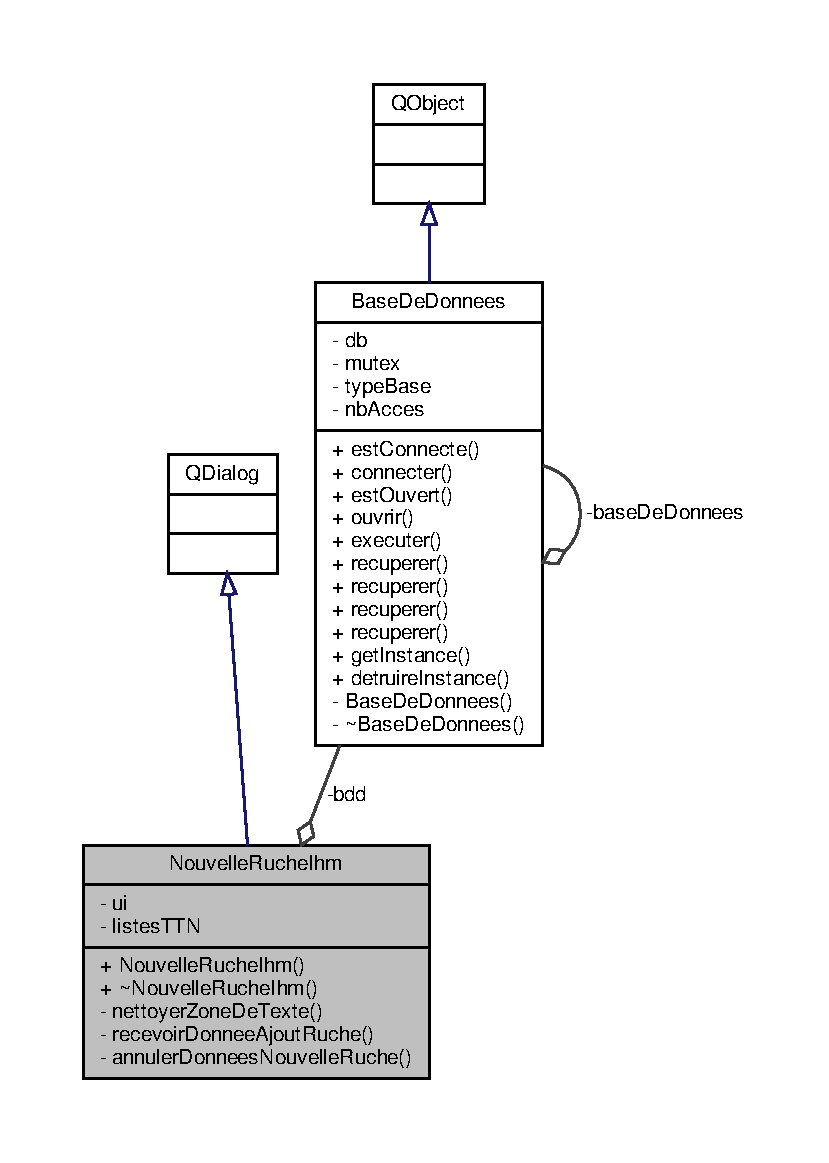
\includegraphics[width=350pt]{class_nouvelle_ruche_ihm__coll__graph}
\end{center}
\end{figure}
\subsubsection*{Fonctions membres publiques}
\begin{DoxyCompactItemize}
\item 
\hyperlink{class_nouvelle_ruche_ihm_a338b9af0b96ed0839a8d5008c8c89cc4}{Nouvelle\+Ruche\+Ihm} (\hyperlink{class_q_widget}{Q\+Widget} $\ast$parent=0)
\begin{DoxyCompactList}\small\item\em Constructeur de la fenêtre principale. \end{DoxyCompactList}\item 
\hyperlink{class_nouvelle_ruche_ihm_a17e5dfd1146574134eaa3ab8eae4f6d4}{$\sim$\+Nouvelle\+Ruche\+Ihm} ()
\begin{DoxyCompactList}\small\item\em Destructeur de la fenêtre principale. \end{DoxyCompactList}\end{DoxyCompactItemize}
\subsubsection*{Connecteurs privés}
\begin{DoxyCompactItemize}
\item 
void \hyperlink{class_nouvelle_ruche_ihm_a268e781b033f2531ca5eab19cc828fdc}{recevoir\+Donnee\+Ajout\+Ruche} ()
\begin{DoxyCompactList}\small\item\em slot permetant l\textquotesingle{}emission des données rentrées par l\textquotesingle{}utilisateur \end{DoxyCompactList}\item 
void \hyperlink{class_nouvelle_ruche_ihm_a8967974b5606b7096960f3b607b5b58a}{annuler\+Donnees\+Nouvelle\+Ruche} ()
\begin{DoxyCompactList}\small\item\em slot permetant grâce a la methode nettoyer\+Zone\+De\+Texte d\textquotesingle{}anuler la saisi des lors que l\textquotesingle{}on appui sur le bouton annuler \end{DoxyCompactList}\end{DoxyCompactItemize}
\subsubsection*{Fonctions membres privées}
\begin{DoxyCompactItemize}
\item 
void \hyperlink{class_nouvelle_ruche_ihm_a09ddd61a2bd2b6779865e7d3b93ec2eb}{nettoyer\+Zone\+De\+Texte} ()
\begin{DoxyCompactList}\small\item\em methode qui clear les zones de textes \end{DoxyCompactList}\end{DoxyCompactItemize}
\subsubsection*{Attributs privés}
\begin{DoxyCompactItemize}
\item 
Ui\+::\+Nouvelle\+Ruche\+Ihm $\ast$ \hyperlink{class_nouvelle_ruche_ihm_a46c1f0446fc75c67847d152d89d75960}{ui}
\item 
\hyperlink{class_base_de_donnees}{Base\+De\+Donnees} $\ast$ \hyperlink{class_nouvelle_ruche_ihm_af552d9e6944c266060860d911878cff7}{bdd}
\begin{DoxyCompactList}\small\item\em agrégation de l\textquotesingle{}objet \hyperlink{class_base_de_donnees}{Base\+De\+Donnees} \end{DoxyCompactList}\item 
Q\+Vector$<$ Q\+String\+List $>$ \hyperlink{class_nouvelle_ruche_ihm_a0c97db3419bafe928aabed3aa01d46fb}{listes\+T\+TN}
\end{DoxyCompactItemize}


\subsubsection{Description détaillée}
\begin{DoxyAuthor}{Auteur}
Florentin Mellah, Enzo Rossi
\end{DoxyAuthor}
\begin{DoxyVersion}{Version}
1.\+1 
\end{DoxyVersion}


\subsubsection{Documentation des constructeurs et destructeur}
\mbox{\Hypertarget{class_nouvelle_ruche_ihm_a338b9af0b96ed0839a8d5008c8c89cc4}\label{class_nouvelle_ruche_ihm_a338b9af0b96ed0839a8d5008c8c89cc4}} 
\index{Nouvelle\+Ruche\+Ihm@{Nouvelle\+Ruche\+Ihm}!Nouvelle\+Ruche\+Ihm@{Nouvelle\+Ruche\+Ihm}}
\index{Nouvelle\+Ruche\+Ihm@{Nouvelle\+Ruche\+Ihm}!Nouvelle\+Ruche\+Ihm@{Nouvelle\+Ruche\+Ihm}}
\paragraph{\texorpdfstring{Nouvelle\+Ruche\+Ihm()}{NouvelleRucheIhm()}}
{\footnotesize\ttfamily Nouvelle\+Ruche\+Ihm\+::\+Nouvelle\+Ruche\+Ihm (\begin{DoxyParamCaption}\item[{\hyperlink{class_q_widget}{Q\+Widget} $\ast$}]{parent = {\ttfamily 0} }\end{DoxyParamCaption})\hspace{0.3cm}{\ttfamily [explicit]}}


\begin{DoxyParams}{Paramètres}
{\em parent} & \hyperlink{class_q_object}{Q\+Object} Adresse de l\textquotesingle{}objet Qt parent (0 = fenêtre principale) \\
\hline
\end{DoxyParams}


Références \hyperlink{class_nouvelle_ruche_ihm_a8967974b5606b7096960f3b607b5b58a}{annuler\+Donnees\+Nouvelle\+Ruche()}, \hyperlink{class_nouvelle_ruche_ihm_af552d9e6944c266060860d911878cff7}{bdd}, \hyperlink{parametres_8h_a45f8f15b8f9a7ab4c2b219038ff64f6b}{B\+D\+D\+\_\+\+N\+O\+M\+B\+A\+SE}, \hyperlink{parametres_8h_ae2ded9166ed2553182545e97514c04f7}{B\+D\+D\+\_\+\+P\+A\+S\+S\+W\+O\+RD}, \hyperlink{parametres_8h_a423559dc987673b8aacaa9f369839bb0}{B\+D\+D\+\_\+\+S\+E\+R\+V\+E\+UR}, \hyperlink{parametres_8h_a88b5f5b81fa534553c68802384beff2c}{B\+D\+D\+\_\+\+U\+S\+E\+R\+N\+A\+ME}, \hyperlink{class_base_de_donnees_ac20da193923a9bfea5e38ee5a54820cd}{Base\+De\+Donnees\+::connecter()}, \hyperlink{class_base_de_donnees_a00388973f3ec42e5c8e76e7af7e124b2}{Base\+De\+Donnees\+::est\+Connecte()}, \hyperlink{class_base_de_donnees_a80028aa2b6b4fbf30fb2e36357b7d3d3}{Base\+De\+Donnees\+::get\+Instance()}, \hyperlink{class_nouvelle_ruche_ihm_a0c97db3419bafe928aabed3aa01d46fb}{listes\+T\+TN}, \hyperlink{class_nouvelle_ruche_ihm_a268e781b033f2531ca5eab19cc828fdc}{recevoir\+Donnee\+Ajout\+Ruche()}, \hyperlink{class_base_de_donnees_a77539baad389f5acf754cd2cd452403e}{Base\+De\+Donnees\+::recuperer()}, et \hyperlink{class_nouvelle_ruche_ihm_a46c1f0446fc75c67847d152d89d75960}{ui}.


\begin{DoxyCode}
00025                                                   :
00026     \hyperlink{class_q_dialog}{QDialog}(parent),
00027     \hyperlink{class_nouvelle_ruche_ihm_a46c1f0446fc75c67847d152d89d75960}{ui}(\textcolor{keyword}{new} Ui::NouvelleRucheIhm)
00028 \{
00029     qDebug()<< Q\_FUNC\_INFO;
00030     \hyperlink{class_nouvelle_ruche_ihm_a46c1f0446fc75c67847d152d89d75960}{ui}->setupUi(\textcolor{keyword}{this});
00031     setWindowTitle(\textcolor{stringliteral}{"Ruche 2019 - Création d'une ruche"});
00032 
00033     \hyperlink{class_nouvelle_ruche_ihm_af552d9e6944c266060860d911878cff7}{bdd} = \hyperlink{class_base_de_donnees_a80028aa2b6b4fbf30fb2e36357b7d3d3}{BaseDeDonnees::getInstance}();
00034     \textcolor{keywordflow}{if}(!\hyperlink{class_nouvelle_ruche_ihm_af552d9e6944c266060860d911878cff7}{bdd}->\hyperlink{class_base_de_donnees_a00388973f3ec42e5c8e76e7af7e124b2}{estConnecte}())
00035         \hyperlink{class_nouvelle_ruche_ihm_af552d9e6944c266060860d911878cff7}{bdd}->\hyperlink{class_base_de_donnees_ac20da193923a9bfea5e38ee5a54820cd}{connecter}(\hyperlink{parametres_8h_a45f8f15b8f9a7ab4c2b219038ff64f6b}{BDD\_NOMBASE}, \hyperlink{parametres_8h_a88b5f5b81fa534553c68802384beff2c}{BDD\_USERNAME}, 
      \hyperlink{parametres_8h_ae2ded9166ed2553182545e97514c04f7}{BDD\_PASSWORD}, \hyperlink{parametres_8h_a423559dc987673b8aacaa9f369839bb0}{BDD\_SERVEUR});
00036 
00037     \textcolor{keywordflow}{if}(\hyperlink{class_nouvelle_ruche_ihm_af552d9e6944c266060860d911878cff7}{bdd}->\hyperlink{class_base_de_donnees_a00388973f3ec42e5c8e76e7af7e124b2}{estConnecte}())
00038     \{
00039         \textcolor{comment}{// Une ruche correspond à un DeviceId attaché à un ApplicationID dans le réseau TTN}
00040         \textcolor{comment}{// récupération des ApplicationID disponibles}
00041         QString requeteRecuperationIdTTN = \textcolor{stringliteral}{"SELECT idTTN, ApplicationID FROM TTN"};
00042         \textcolor{keywordtype}{bool} retourRequeteRecuperationIdTTN = \hyperlink{class_nouvelle_ruche_ihm_af552d9e6944c266060860d911878cff7}{bdd}->\hyperlink{class_base_de_donnees_a77539baad389f5acf754cd2cd452403e}{recuperer}(requeteRecuperationIdTTN, 
      \hyperlink{class_nouvelle_ruche_ihm_a0c97db3419bafe928aabed3aa01d46fb}{listesTTN});
00043         \textcolor{keywordflow}{if}(retourRequeteRecuperationIdTTN)
00044         \{
00045             \textcolor{keywordflow}{for}(\textcolor{keywordtype}{int} i=0;i<\hyperlink{class_nouvelle_ruche_ihm_a0c97db3419bafe928aabed3aa01d46fb}{listesTTN}.size();i++)
00046             \{
00047                 \hyperlink{class_nouvelle_ruche_ihm_a46c1f0446fc75c67847d152d89d75960}{ui}->comboBoxListeAppID->addItem(\hyperlink{class_nouvelle_ruche_ihm_a0c97db3419bafe928aabed3aa01d46fb}{listesTTN}.at(i).at(1));
00048             \}
00049         \}
00050         \textcolor{keywordflow}{else}
00051             \hyperlink{class_nouvelle_ruche_ihm_a46c1f0446fc75c67847d152d89d75960}{ui}->comboBoxListeAppID->addItem(\textcolor{stringliteral}{""});
00052     \}
00053 
00054     QDate aujourdhui = QDate::currentDate();
00055     \hyperlink{class_nouvelle_ruche_ihm_a46c1f0446fc75c67847d152d89d75960}{ui}->dateEditMiseEnService->setDate(aujourdhui);
00056 
00057     connect(\hyperlink{class_nouvelle_ruche_ihm_a46c1f0446fc75c67847d152d89d75960}{ui}->boutonOk,SIGNAL(clicked(\textcolor{keywordtype}{bool})),\textcolor{keyword}{this},SLOT(
      \hyperlink{class_nouvelle_ruche_ihm_a268e781b033f2531ca5eab19cc828fdc}{recevoirDonneeAjoutRuche}()));
00058     connect(\hyperlink{class_nouvelle_ruche_ihm_a46c1f0446fc75c67847d152d89d75960}{ui}->boutonAnnuler,SIGNAL(clicked(\textcolor{keywordtype}{bool})),\textcolor{keyword}{this},SLOT(
      \hyperlink{class_nouvelle_ruche_ihm_a8967974b5606b7096960f3b607b5b58a}{annulerDonneesNouvelleRuche}()));
00059 \}
\end{DoxyCode}
\mbox{\Hypertarget{class_nouvelle_ruche_ihm_a17e5dfd1146574134eaa3ab8eae4f6d4}\label{class_nouvelle_ruche_ihm_a17e5dfd1146574134eaa3ab8eae4f6d4}} 
\index{Nouvelle\+Ruche\+Ihm@{Nouvelle\+Ruche\+Ihm}!````~Nouvelle\+Ruche\+Ihm@{$\sim$\+Nouvelle\+Ruche\+Ihm}}
\index{````~Nouvelle\+Ruche\+Ihm@{$\sim$\+Nouvelle\+Ruche\+Ihm}!Nouvelle\+Ruche\+Ihm@{Nouvelle\+Ruche\+Ihm}}
\paragraph{\texorpdfstring{$\sim$\+Nouvelle\+Ruche\+Ihm()}{~NouvelleRucheIhm()}}
{\footnotesize\ttfamily Nouvelle\+Ruche\+Ihm\+::$\sim$\+Nouvelle\+Ruche\+Ihm (\begin{DoxyParamCaption}{ }\end{DoxyParamCaption})}



Références \hyperlink{class_base_de_donnees_a457401c0816b888c77ce915997545f4e}{Base\+De\+Donnees\+::detruire\+Instance()}, et \hyperlink{class_nouvelle_ruche_ihm_a46c1f0446fc75c67847d152d89d75960}{ui}.


\begin{DoxyCode}
00068 \{
00069     \textcolor{keyword}{delete} \hyperlink{class_nouvelle_ruche_ihm_a46c1f0446fc75c67847d152d89d75960}{ui};
00070     \hyperlink{class_base_de_donnees_a457401c0816b888c77ce915997545f4e}{BaseDeDonnees::detruireInstance}();
00071 \}
\end{DoxyCode}


\subsubsection{Documentation des fonctions membres}
\mbox{\Hypertarget{class_nouvelle_ruche_ihm_a8967974b5606b7096960f3b607b5b58a}\label{class_nouvelle_ruche_ihm_a8967974b5606b7096960f3b607b5b58a}} 
\index{Nouvelle\+Ruche\+Ihm@{Nouvelle\+Ruche\+Ihm}!annuler\+Donnees\+Nouvelle\+Ruche@{annuler\+Donnees\+Nouvelle\+Ruche}}
\index{annuler\+Donnees\+Nouvelle\+Ruche@{annuler\+Donnees\+Nouvelle\+Ruche}!Nouvelle\+Ruche\+Ihm@{Nouvelle\+Ruche\+Ihm}}
\paragraph{\texorpdfstring{annuler\+Donnees\+Nouvelle\+Ruche}{annulerDonneesNouvelleRuche}}
{\footnotesize\ttfamily void Nouvelle\+Ruche\+Ihm\+::annuler\+Donnees\+Nouvelle\+Ruche (\begin{DoxyParamCaption}{ }\end{DoxyParamCaption})\hspace{0.3cm}{\ttfamily [private]}, {\ttfamily [slot]}}



Références \hyperlink{class_nouvelle_ruche_ihm_a09ddd61a2bd2b6779865e7d3b93ec2eb}{nettoyer\+Zone\+De\+Texte()}.



Référencé par \hyperlink{class_nouvelle_ruche_ihm_a338b9af0b96ed0839a8d5008c8c89cc4}{Nouvelle\+Ruche\+Ihm()}.


\begin{DoxyCode}
00113 \{
00114     \hyperlink{class_nouvelle_ruche_ihm_a09ddd61a2bd2b6779865e7d3b93ec2eb}{nettoyerZoneDeTexte}();
00115     reject();
00116 \}
\end{DoxyCode}
\mbox{\Hypertarget{class_nouvelle_ruche_ihm_a09ddd61a2bd2b6779865e7d3b93ec2eb}\label{class_nouvelle_ruche_ihm_a09ddd61a2bd2b6779865e7d3b93ec2eb}} 
\index{Nouvelle\+Ruche\+Ihm@{Nouvelle\+Ruche\+Ihm}!nettoyer\+Zone\+De\+Texte@{nettoyer\+Zone\+De\+Texte}}
\index{nettoyer\+Zone\+De\+Texte@{nettoyer\+Zone\+De\+Texte}!Nouvelle\+Ruche\+Ihm@{Nouvelle\+Ruche\+Ihm}}
\paragraph{\texorpdfstring{nettoyer\+Zone\+De\+Texte()}{nettoyerZoneDeTexte()}}
{\footnotesize\ttfamily void Nouvelle\+Ruche\+Ihm\+::nettoyer\+Zone\+De\+Texte (\begin{DoxyParamCaption}{ }\end{DoxyParamCaption})\hspace{0.3cm}{\ttfamily [private]}}



Références \hyperlink{class_nouvelle_ruche_ihm_a46c1f0446fc75c67847d152d89d75960}{ui}.



Référencé par \hyperlink{class_nouvelle_ruche_ihm_a8967974b5606b7096960f3b607b5b58a}{annuler\+Donnees\+Nouvelle\+Ruche()}, et \hyperlink{class_nouvelle_ruche_ihm_a268e781b033f2531ca5eab19cc828fdc}{recevoir\+Donnee\+Ajout\+Ruche()}.


\begin{DoxyCode}
00124 \{
00125     \hyperlink{class_nouvelle_ruche_ihm_a46c1f0446fc75c67847d152d89d75960}{ui}->zoneDeTexteNom->clear();
00126     \hyperlink{class_nouvelle_ruche_ihm_a46c1f0446fc75c67847d152d89d75960}{ui}->zoneDeTexteDescription->clear();
00127     \hyperlink{class_nouvelle_ruche_ihm_a46c1f0446fc75c67847d152d89d75960}{ui}->zoneDeTexteAdresse->clear();
00128     \hyperlink{class_nouvelle_ruche_ihm_a46c1f0446fc75c67847d152d89d75960}{ui}->zoneDeTexteLongitude->clear();
00129     \hyperlink{class_nouvelle_ruche_ihm_a46c1f0446fc75c67847d152d89d75960}{ui}->zoneDeTexteLatitude->clear();
00130     \hyperlink{class_nouvelle_ruche_ihm_a46c1f0446fc75c67847d152d89d75960}{ui}->zoneDeTexteDeviceID->clear();
00131 \}
\end{DoxyCode}
\mbox{\Hypertarget{class_nouvelle_ruche_ihm_a268e781b033f2531ca5eab19cc828fdc}\label{class_nouvelle_ruche_ihm_a268e781b033f2531ca5eab19cc828fdc}} 
\index{Nouvelle\+Ruche\+Ihm@{Nouvelle\+Ruche\+Ihm}!recevoir\+Donnee\+Ajout\+Ruche@{recevoir\+Donnee\+Ajout\+Ruche}}
\index{recevoir\+Donnee\+Ajout\+Ruche@{recevoir\+Donnee\+Ajout\+Ruche}!Nouvelle\+Ruche\+Ihm@{Nouvelle\+Ruche\+Ihm}}
\paragraph{\texorpdfstring{recevoir\+Donnee\+Ajout\+Ruche}{recevoirDonneeAjoutRuche}}
{\footnotesize\ttfamily void Nouvelle\+Ruche\+Ihm\+::recevoir\+Donnee\+Ajout\+Ruche (\begin{DoxyParamCaption}{ }\end{DoxyParamCaption})\hspace{0.3cm}{\ttfamily [private]}, {\ttfamily [slot]}}



Références \hyperlink{parametres_8h_ace364d1ce44aa9f79bcff6e3752c4a5f}{A\+P\+P\+\_\+\+T\+I\+T\+RE}, \hyperlink{class_nouvelle_ruche_ihm_af552d9e6944c266060860d911878cff7}{bdd}, \hyperlink{class_base_de_donnees_aa8de5f8f8bb17edc43f5c0ee33712081}{Base\+De\+Donnees\+::executer()}, \hyperlink{class_nouvelle_ruche_ihm_a0c97db3419bafe928aabed3aa01d46fb}{listes\+T\+TN}, \hyperlink{class_nouvelle_ruche_ihm_a09ddd61a2bd2b6779865e7d3b93ec2eb}{nettoyer\+Zone\+De\+Texte()}, \hyperlink{class_base_de_donnees_a77539baad389f5acf754cd2cd452403e}{Base\+De\+Donnees\+::recuperer()}, et \hyperlink{class_nouvelle_ruche_ihm_a46c1f0446fc75c67847d152d89d75960}{ui}.



Référencé par \hyperlink{class_nouvelle_ruche_ihm_a338b9af0b96ed0839a8d5008c8c89cc4}{Nouvelle\+Ruche\+Ihm()}.


\begin{DoxyCode}
00079 \{
00080     \textcolor{keywordflow}{if}(\hyperlink{class_nouvelle_ruche_ihm_a0c97db3419bafe928aabed3aa01d46fb}{listesTTN}.size() == 0)
00081     \{
00082         QMessageBox::critical(0, QString::fromUtf8(\hyperlink{parametres_8h_ace364d1ce44aa9f79bcff6e3752c4a5f}{APP\_TITRE}), QString::fromUtf8(\textcolor{stringliteral}{"Impossible
       d'ajouter la nouvelle ruche : TTN manquant !"}));
00083         \textcolor{keywordflow}{return};
00084     \}
00085 
00086     QDate date = QDate::fromString(\hyperlink{class_nouvelle_ruche_ihm_a46c1f0446fc75c67847d152d89d75960}{ui}->dateEditMiseEnService->text(), \textcolor{stringliteral}{"dd/MM/yyyy"});
00087     QString requete = \textcolor{stringliteral}{"INSERT INTO Ruche (idTTN, Nom, Description, DateMiseEnService, Adresse, Longitude,
       Latitude, DeviceID) VALUES ('"} + \hyperlink{class_nouvelle_ruche_ihm_a0c97db3419bafe928aabed3aa01d46fb}{listesTTN}.at(\hyperlink{class_nouvelle_ruche_ihm_a46c1f0446fc75c67847d152d89d75960}{ui}->comboBoxListeAppID->currentIndex()).at(0) + \textcolor{stringliteral}{"' ,
       '"} + \hyperlink{class_nouvelle_ruche_ihm_a46c1f0446fc75c67847d152d89d75960}{ui}->zoneDeTexteNom->text() + \textcolor{stringliteral}{"', '"} + \hyperlink{class_nouvelle_ruche_ihm_a46c1f0446fc75c67847d152d89d75960}{ui}->zoneDeTexteDescription->text() + \textcolor{stringliteral}{"', '"} + date.toString(\textcolor{stringliteral}{
      "yyyy-MM-dd"}) + \textcolor{stringliteral}{"', '"} + \hyperlink{class_nouvelle_ruche_ihm_a46c1f0446fc75c67847d152d89d75960}{ui}->zoneDeTexteAdresse->text() + \textcolor{stringliteral}{"', '"} + \hyperlink{class_nouvelle_ruche_ihm_a46c1f0446fc75c67847d152d89d75960}{ui}->zoneDeTexteLongitude->text() + \textcolor{stringliteral}{"
      ', '"} + \hyperlink{class_nouvelle_ruche_ihm_a46c1f0446fc75c67847d152d89d75960}{ui}->zoneDeTexteLatitude->text() + \textcolor{stringliteral}{"', '"} + \hyperlink{class_nouvelle_ruche_ihm_a46c1f0446fc75c67847d152d89d75960}{ui}->zoneDeTexteDeviceID->text() + \textcolor{stringliteral}{"')"};
00088     qDebug()<< Q\_FUNC\_INFO << requete;
00089     \textcolor{keywordtype}{bool} retour = \hyperlink{class_nouvelle_ruche_ihm_af552d9e6944c266060860d911878cff7}{bdd}->\hyperlink{class_base_de_donnees_aa8de5f8f8bb17edc43f5c0ee33712081}{executer}(requete);
00090     \textcolor{keywordflow}{if}(retour)
00091     \{
00092         QString idRuche;
00093         requete = \textcolor{stringliteral}{"SELECT idRuche FROM Ruche WHERE DeviceID='"} + \hyperlink{class_nouvelle_ruche_ihm_a46c1f0446fc75c67847d152d89d75960}{ui}->zoneDeTexteDeviceID->text() + \textcolor{stringliteral}{"'"};
00094         retour = \hyperlink{class_nouvelle_ruche_ihm_af552d9e6944c266060860d911878cff7}{bdd}->\hyperlink{class_base_de_donnees_a77539baad389f5acf754cd2cd452403e}{recuperer}(requete, idRuche);
00095         \textcolor{keywordflow}{if}(retour)
00096         \{
00097             requete = \textcolor{stringliteral}{"INSERT INTO Seuils (idRuche, TemperatureIntMin, TemperatureIntMax, HumiditeIntMin,
       HumiditeIntMax, TemperatureExtMin, TemperatureExtMax, HumiditeExtMin, HumiditeExtMax, PressionMin,
       PressionMax, PoidsMin, PoidsMax, EnsoleillementMin, EnsoleillementMax, Charge) VALUES ('"} + idRuche + \textcolor{stringliteral}{"' , '"} + \textcolor{stringliteral}{"25."} 
      + \textcolor{stringliteral}{"', '"} + \textcolor{stringliteral}{"35.0"} + \textcolor{stringliteral}{"', '"} + \textcolor{stringliteral}{"20"} + \textcolor{stringliteral}{"', '"} + \textcolor{stringliteral}{"30"} + \textcolor{stringliteral}{"', '"} + \textcolor{stringliteral}{"5"} + \textcolor{stringliteral}{"', '"} + \textcolor{stringliteral}{"35"} + \textcolor{stringliteral}{"', '"} + \textcolor{stringliteral}{"20"} + \textcolor{stringliteral}{"', '"} + \textcolor{stringliteral}{
      "35"} + \textcolor{stringliteral}{"', '"} + \textcolor{stringliteral}{"1000"} + \textcolor{stringliteral}{"', '"} + \textcolor{stringliteral}{"1200"} + \textcolor{stringliteral}{"', '"} + \textcolor{stringliteral}{"10"} + \textcolor{stringliteral}{"', '"} + \textcolor{stringliteral}{"100"} + \textcolor{stringliteral}{"', '"} + \textcolor{stringliteral}{"10"} + \textcolor{stringliteral}{"', '"} + \textcolor{stringliteral}{"1000"} 
      + \textcolor{stringliteral}{"', '"} + \textcolor{stringliteral}{"25"} + \textcolor{stringliteral}{"')"};
00098             retour = \hyperlink{class_nouvelle_ruche_ihm_af552d9e6944c266060860d911878cff7}{bdd}->\hyperlink{class_base_de_donnees_aa8de5f8f8bb17edc43f5c0ee33712081}{executer}(requete);
00099         \}
00100         \hyperlink{class_nouvelle_ruche_ihm_a09ddd61a2bd2b6779865e7d3b93ec2eb}{nettoyerZoneDeTexte}();
00101         accept();
00102     \}
00103     \textcolor{keywordflow}{else}
00104         QMessageBox::critical(0, QString::fromUtf8(\hyperlink{parametres_8h_ace364d1ce44aa9f79bcff6e3752c4a5f}{APP\_TITRE}), QString::fromUtf8(\textcolor{stringliteral}{"Impossible
       d'ajouter la nouvelle ruche !"}));
00105 \}
\end{DoxyCode}


\subsubsection{Documentation des données membres}
\mbox{\Hypertarget{class_nouvelle_ruche_ihm_af552d9e6944c266060860d911878cff7}\label{class_nouvelle_ruche_ihm_af552d9e6944c266060860d911878cff7}} 
\index{Nouvelle\+Ruche\+Ihm@{Nouvelle\+Ruche\+Ihm}!bdd@{bdd}}
\index{bdd@{bdd}!Nouvelle\+Ruche\+Ihm@{Nouvelle\+Ruche\+Ihm}}
\paragraph{\texorpdfstring{bdd}{bdd}}
{\footnotesize\ttfamily \hyperlink{class_base_de_donnees}{Base\+De\+Donnees}$\ast$ Nouvelle\+Ruche\+Ihm\+::bdd\hspace{0.3cm}{\ttfamily [private]}}



Référencé par \hyperlink{class_nouvelle_ruche_ihm_a338b9af0b96ed0839a8d5008c8c89cc4}{Nouvelle\+Ruche\+Ihm()}, et \hyperlink{class_nouvelle_ruche_ihm_a268e781b033f2531ca5eab19cc828fdc}{recevoir\+Donnee\+Ajout\+Ruche()}.

\mbox{\Hypertarget{class_nouvelle_ruche_ihm_a0c97db3419bafe928aabed3aa01d46fb}\label{class_nouvelle_ruche_ihm_a0c97db3419bafe928aabed3aa01d46fb}} 
\index{Nouvelle\+Ruche\+Ihm@{Nouvelle\+Ruche\+Ihm}!listes\+T\+TN@{listes\+T\+TN}}
\index{listes\+T\+TN@{listes\+T\+TN}!Nouvelle\+Ruche\+Ihm@{Nouvelle\+Ruche\+Ihm}}
\paragraph{\texorpdfstring{listes\+T\+TN}{listesTTN}}
{\footnotesize\ttfamily Q\+Vector$<$Q\+String\+List$>$ Nouvelle\+Ruche\+Ihm\+::listes\+T\+TN\hspace{0.3cm}{\ttfamily [private]}}



Référencé par \hyperlink{class_nouvelle_ruche_ihm_a338b9af0b96ed0839a8d5008c8c89cc4}{Nouvelle\+Ruche\+Ihm()}, et \hyperlink{class_nouvelle_ruche_ihm_a268e781b033f2531ca5eab19cc828fdc}{recevoir\+Donnee\+Ajout\+Ruche()}.

\mbox{\Hypertarget{class_nouvelle_ruche_ihm_a46c1f0446fc75c67847d152d89d75960}\label{class_nouvelle_ruche_ihm_a46c1f0446fc75c67847d152d89d75960}} 
\index{Nouvelle\+Ruche\+Ihm@{Nouvelle\+Ruche\+Ihm}!ui@{ui}}
\index{ui@{ui}!Nouvelle\+Ruche\+Ihm@{Nouvelle\+Ruche\+Ihm}}
\paragraph{\texorpdfstring{ui}{ui}}
{\footnotesize\ttfamily Ui\+::\+Nouvelle\+Ruche\+Ihm$\ast$ Nouvelle\+Ruche\+Ihm\+::ui\hspace{0.3cm}{\ttfamily [private]}}



Référencé par \hyperlink{class_nouvelle_ruche_ihm_a09ddd61a2bd2b6779865e7d3b93ec2eb}{nettoyer\+Zone\+De\+Texte()}, \hyperlink{class_nouvelle_ruche_ihm_a338b9af0b96ed0839a8d5008c8c89cc4}{Nouvelle\+Ruche\+Ihm()}, \hyperlink{class_nouvelle_ruche_ihm_a268e781b033f2531ca5eab19cc828fdc}{recevoir\+Donnee\+Ajout\+Ruche()}, et \hyperlink{class_nouvelle_ruche_ihm_a17e5dfd1146574134eaa3ab8eae4f6d4}{$\sim$\+Nouvelle\+Ruche\+Ihm()}.



La documentation de cette classe a été générée à partir des fichiers suivants \+:\begin{DoxyCompactItemize}
\item 
\hyperlink{nouvelle_ruche_ihm_8h}{nouvelle\+Ruche\+Ihm.\+h}\item 
\hyperlink{nouvelle_ruche_ihm_8cpp}{nouvelle\+Ruche\+Ihm.\+cpp}\end{DoxyCompactItemize}

\hypertarget{classfr_1_1campus_1_1laurainc_1_1honeybee_1_1_parametres_honey_bee_activity}{}\subsection{Référence de la classe fr.\+campus.\+laurainc.\+honeybee.\+Parametres\+Honey\+Bee\+Activity}
\label{classfr_1_1campus_1_1laurainc_1_1honeybee_1_1_parametres_honey_bee_activity}\index{fr.\+campus.\+laurainc.\+honeybee.\+Parametres\+Honey\+Bee\+Activity@{fr.\+campus.\+laurainc.\+honeybee.\+Parametres\+Honey\+Bee\+Activity}}


Activité de paramétrage de l\textquotesingle{}application.  




Graphe de collaboration de fr.\+campus.\+laurainc.\+honeybee.\+Parametres\+Honey\+Bee\+Activity\+:\nopagebreak
\begin{figure}[H]
\begin{center}
\leavevmode
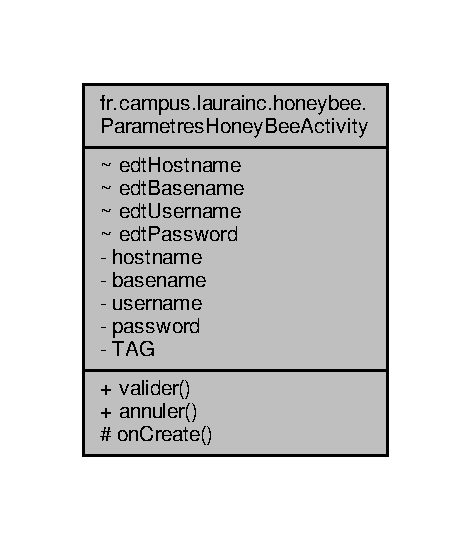
\includegraphics[width=226pt]{classfr_1_1campus_1_1laurainc_1_1honeybee_1_1_parametres_honey_bee_activity__coll__graph}
\end{center}
\end{figure}
\subsubsection*{Fonctions membres publiques}
\begin{DoxyCompactItemize}
\item 
void \hyperlink{classfr_1_1campus_1_1laurainc_1_1honeybee_1_1_parametres_honey_bee_activity_a75d00ffbc312cbbee09bfe4e7d5153c1}{valider} (View view)
\begin{DoxyCompactList}\small\item\em Quitte l\textquotesingle{}activité en appliquant les paramètres. \end{DoxyCompactList}\item 
void \hyperlink{classfr_1_1campus_1_1laurainc_1_1honeybee_1_1_parametres_honey_bee_activity_a1db4c582af1057bf1577b1f7a74ea8fe}{annuler} (View view)
\begin{DoxyCompactList}\small\item\em Quitte l\textquotesingle{}activité sans prendre en compte les paramètres. \end{DoxyCompactList}\end{DoxyCompactItemize}
\subsubsection*{Fonctions membres protégées}
\begin{DoxyCompactItemize}
\item 
void \hyperlink{classfr_1_1campus_1_1laurainc_1_1honeybee_1_1_parametres_honey_bee_activity_a43786040ab7dbe39e90bfc684b4c40f7}{on\+Create} (Bundle saved\+Instance\+State)
\end{DoxyCompactItemize}
\subsubsection*{Attributs privés}
\begin{DoxyCompactItemize}
\item 
String \hyperlink{classfr_1_1campus_1_1laurainc_1_1honeybee_1_1_parametres_honey_bee_activity_abe6d58e55747fe47a9d440b925c50f0d}{hostname}
\begin{DoxyCompactList}\small\item\em l\textquotesingle{}adress IP du serveur My\+S\+QL \end{DoxyCompactList}\item 
String \hyperlink{classfr_1_1campus_1_1laurainc_1_1honeybee_1_1_parametres_honey_bee_activity_aaccd793d1d2883ca9471fe783915a9de}{basename} = \char`\"{}ruche\char`\"{}
\begin{DoxyCompactList}\small\item\em le nom de la la base de données du serveur My\+S\+QL \end{DoxyCompactList}\item 
String \hyperlink{classfr_1_1campus_1_1laurainc_1_1honeybee_1_1_parametres_honey_bee_activity_a91b281cedd628be41899059c32a4fe03}{username} = \char`\"{}root\char`\"{}
\begin{DoxyCompactList}\small\item\em le nom du compte utilisateur (root par défaut) \end{DoxyCompactList}\item 
String \hyperlink{classfr_1_1campus_1_1laurainc_1_1honeybee_1_1_parametres_honey_bee_activity_a040c25d676f0391af65c55349575bc66}{password} = \char`\"{}password\char`\"{}
\begin{DoxyCompactList}\small\item\em le mot de passe du compte utilisateur (password par défaut) \end{DoxyCompactList}\end{DoxyCompactItemize}
\subsubsection*{Attributs privés statiques}
\begin{DoxyCompactItemize}
\item 
static final String \hyperlink{classfr_1_1campus_1_1laurainc_1_1honeybee_1_1_parametres_honey_bee_activity_a9fcf6f5bb050914a6f719f04870f1494}{T\+AG} = \char`\"{}Parametres\+Honey\+Bee\+Activity\char`\"{}
\begin{DoxyCompactList}\small\item\em le T\+AG de la classe pour les logs \end{DoxyCompactList}\end{DoxyCompactItemize}


\subsubsection{Description détaillée}
\begin{DoxyRefDesc}{A faire}
\item[\hyperlink{todo__todo000004}{A faire}]D\textquotesingle{}autres paramètres ? M\+Q\+TT ? ... \end{DoxyRefDesc}


\subsubsection{Documentation des fonctions membres}
\mbox{\Hypertarget{classfr_1_1campus_1_1laurainc_1_1honeybee_1_1_parametres_honey_bee_activity_a1db4c582af1057bf1577b1f7a74ea8fe}\label{classfr_1_1campus_1_1laurainc_1_1honeybee_1_1_parametres_honey_bee_activity_a1db4c582af1057bf1577b1f7a74ea8fe}} 
\index{fr\+::campus\+::laurainc\+::honeybee\+::\+Parametres\+Honey\+Bee\+Activity@{fr\+::campus\+::laurainc\+::honeybee\+::\+Parametres\+Honey\+Bee\+Activity}!annuler@{annuler}}
\index{annuler@{annuler}!fr\+::campus\+::laurainc\+::honeybee\+::\+Parametres\+Honey\+Bee\+Activity@{fr\+::campus\+::laurainc\+::honeybee\+::\+Parametres\+Honey\+Bee\+Activity}}
\paragraph{\texorpdfstring{annuler()}{annuler()}}
{\footnotesize\ttfamily fr.\+campus.\+laurainc.\+honeybee.\+Parametres\+Honey\+Bee\+Activity.\+annuler (\begin{DoxyParamCaption}\item[{View}]{view }\end{DoxyParamCaption})}


\begin{DoxyParams}{Paramètres}
{\em view} & View la vue associée \\
\hline
\end{DoxyParams}

\begin{DoxyCode}
00078     \{
00079         Intent intent = \textcolor{keyword}{new} Intent();
00080         setResult(RESULT\_CANCELED, intent);
00081         finish();
00082     \}
\end{DoxyCode}
\mbox{\Hypertarget{classfr_1_1campus_1_1laurainc_1_1honeybee_1_1_parametres_honey_bee_activity_a43786040ab7dbe39e90bfc684b4c40f7}\label{classfr_1_1campus_1_1laurainc_1_1honeybee_1_1_parametres_honey_bee_activity_a43786040ab7dbe39e90bfc684b4c40f7}} 
\index{fr\+::campus\+::laurainc\+::honeybee\+::\+Parametres\+Honey\+Bee\+Activity@{fr\+::campus\+::laurainc\+::honeybee\+::\+Parametres\+Honey\+Bee\+Activity}!on\+Create@{on\+Create}}
\index{on\+Create@{on\+Create}!fr\+::campus\+::laurainc\+::honeybee\+::\+Parametres\+Honey\+Bee\+Activity@{fr\+::campus\+::laurainc\+::honeybee\+::\+Parametres\+Honey\+Bee\+Activity}}
\paragraph{\texorpdfstring{on\+Create()}{onCreate()}}
{\footnotesize\ttfamily void fr.\+campus.\+laurainc.\+honeybee.\+Parametres\+Honey\+Bee\+Activity.\+on\+Create (\begin{DoxyParamCaption}\item[{Bundle}]{saved\+Instance\+State }\end{DoxyParamCaption})\hspace{0.3cm}{\ttfamily [protected]}}


\begin{DoxyCode}
00031     \{
00032         super.onCreate(savedInstanceState);
00033         setContentView(R.layout.activity\_parametres\_honey\_bee);
00034 
00035         Intent intent = getIntent();
00036         \hyperlink{classfr_1_1campus_1_1laurainc_1_1honeybee_1_1_parametres_honey_bee_activity_abe6d58e55747fe47a9d440b925c50f0d}{hostname} = intent.getStringExtra(\textcolor{stringliteral}{"hostname"});
00037         \hyperlink{classfr_1_1campus_1_1laurainc_1_1honeybee_1_1_parametres_honey_bee_activity_aaccd793d1d2883ca9471fe783915a9de}{basename} = intent.getStringExtra(\textcolor{stringliteral}{"basename"});
00038         \hyperlink{classfr_1_1campus_1_1laurainc_1_1honeybee_1_1_parametres_honey_bee_activity_a91b281cedd628be41899059c32a4fe03}{username} = intent.getStringExtra(\textcolor{stringliteral}{"username"});
00039         \hyperlink{classfr_1_1campus_1_1laurainc_1_1honeybee_1_1_parametres_honey_bee_activity_a040c25d676f0391af65c55349575bc66}{password} = intent.getStringExtra(\textcolor{stringliteral}{"password"});
00040 
00041         edtHostname = (EditText) this.findViewById(R.id.edtHostname);
00042         edtBasename = (EditText) this.findViewById(R.id.edtBasename);
00043         edtUsername = (EditText) this.findViewById(R.id.edtUsername);
00044         edtPassword = (EditText) this.findViewById(R.id.edtPassword);
00045 
00046         edtHostname.setText(\hyperlink{classfr_1_1campus_1_1laurainc_1_1honeybee_1_1_parametres_honey_bee_activity_abe6d58e55747fe47a9d440b925c50f0d}{hostname}, TextView.BufferType.EDITABLE);
00047         edtBasename.setText(\hyperlink{classfr_1_1campus_1_1laurainc_1_1honeybee_1_1_parametres_honey_bee_activity_aaccd793d1d2883ca9471fe783915a9de}{basename}, TextView.BufferType.EDITABLE);
00048         edtUsername.setText(\hyperlink{classfr_1_1campus_1_1laurainc_1_1honeybee_1_1_parametres_honey_bee_activity_a91b281cedd628be41899059c32a4fe03}{username}, TextView.BufferType.EDITABLE);
00049         edtPassword.setText(\hyperlink{classfr_1_1campus_1_1laurainc_1_1honeybee_1_1_parametres_honey_bee_activity_a040c25d676f0391af65c55349575bc66}{password}, TextView.BufferType.EDITABLE);
00050     \}
\end{DoxyCode}
\mbox{\Hypertarget{classfr_1_1campus_1_1laurainc_1_1honeybee_1_1_parametres_honey_bee_activity_a75d00ffbc312cbbee09bfe4e7d5153c1}\label{classfr_1_1campus_1_1laurainc_1_1honeybee_1_1_parametres_honey_bee_activity_a75d00ffbc312cbbee09bfe4e7d5153c1}} 
\index{fr\+::campus\+::laurainc\+::honeybee\+::\+Parametres\+Honey\+Bee\+Activity@{fr\+::campus\+::laurainc\+::honeybee\+::\+Parametres\+Honey\+Bee\+Activity}!valider@{valider}}
\index{valider@{valider}!fr\+::campus\+::laurainc\+::honeybee\+::\+Parametres\+Honey\+Bee\+Activity@{fr\+::campus\+::laurainc\+::honeybee\+::\+Parametres\+Honey\+Bee\+Activity}}
\paragraph{\texorpdfstring{valider()}{valider()}}
{\footnotesize\ttfamily fr.\+campus.\+laurainc.\+honeybee.\+Parametres\+Honey\+Bee\+Activity.\+valider (\begin{DoxyParamCaption}\item[{View}]{view }\end{DoxyParamCaption})}


\begin{DoxyParams}{Paramètres}
{\em view} & View la vue associée \\
\hline
\end{DoxyParams}

\begin{DoxyCode}
00058     \{
00059         Intent intent = \textcolor{keyword}{new} Intent();
00060         \hyperlink{classfr_1_1campus_1_1laurainc_1_1honeybee_1_1_parametres_honey_bee_activity_abe6d58e55747fe47a9d440b925c50f0d}{hostname} = edtHostname.getText().toString();
00061         \hyperlink{classfr_1_1campus_1_1laurainc_1_1honeybee_1_1_parametres_honey_bee_activity_aaccd793d1d2883ca9471fe783915a9de}{basename} = edtBasename.getText().toString();
00062         \hyperlink{classfr_1_1campus_1_1laurainc_1_1honeybee_1_1_parametres_honey_bee_activity_a91b281cedd628be41899059c32a4fe03}{username} = edtUsername.getText().toString();
00063         \hyperlink{classfr_1_1campus_1_1laurainc_1_1honeybee_1_1_parametres_honey_bee_activity_a040c25d676f0391af65c55349575bc66}{password} = edtPassword.getText().toString();
00064         intent.putExtra(\textcolor{stringliteral}{"hostname"}, \hyperlink{classfr_1_1campus_1_1laurainc_1_1honeybee_1_1_parametres_honey_bee_activity_abe6d58e55747fe47a9d440b925c50f0d}{hostname});
00065         intent.putExtra(\textcolor{stringliteral}{"basename"}, \hyperlink{classfr_1_1campus_1_1laurainc_1_1honeybee_1_1_parametres_honey_bee_activity_aaccd793d1d2883ca9471fe783915a9de}{basename});
00066         intent.putExtra(\textcolor{stringliteral}{"username"}, \hyperlink{classfr_1_1campus_1_1laurainc_1_1honeybee_1_1_parametres_honey_bee_activity_a91b281cedd628be41899059c32a4fe03}{username});
00067         intent.putExtra(\textcolor{stringliteral}{"password"}, \hyperlink{classfr_1_1campus_1_1laurainc_1_1honeybee_1_1_parametres_honey_bee_activity_a040c25d676f0391af65c55349575bc66}{password});
00068         setResult(RESULT\_OK, intent);
00069         finish();
00070     \}
\end{DoxyCode}


\subsubsection{Documentation des données membres}
\mbox{\Hypertarget{classfr_1_1campus_1_1laurainc_1_1honeybee_1_1_parametres_honey_bee_activity_aaccd793d1d2883ca9471fe783915a9de}\label{classfr_1_1campus_1_1laurainc_1_1honeybee_1_1_parametres_honey_bee_activity_aaccd793d1d2883ca9471fe783915a9de}} 
\index{fr\+::campus\+::laurainc\+::honeybee\+::\+Parametres\+Honey\+Bee\+Activity@{fr\+::campus\+::laurainc\+::honeybee\+::\+Parametres\+Honey\+Bee\+Activity}!basename@{basename}}
\index{basename@{basename}!fr\+::campus\+::laurainc\+::honeybee\+::\+Parametres\+Honey\+Bee\+Activity@{fr\+::campus\+::laurainc\+::honeybee\+::\+Parametres\+Honey\+Bee\+Activity}}
\paragraph{\texorpdfstring{basename}{basename}}
{\footnotesize\ttfamily String fr.\+campus.\+laurainc.\+honeybee.\+Parametres\+Honey\+Bee\+Activity.\+basename = \char`\"{}ruche\char`\"{}\hspace{0.3cm}{\ttfamily [private]}}

\mbox{\Hypertarget{classfr_1_1campus_1_1laurainc_1_1honeybee_1_1_parametres_honey_bee_activity_abe6d58e55747fe47a9d440b925c50f0d}\label{classfr_1_1campus_1_1laurainc_1_1honeybee_1_1_parametres_honey_bee_activity_abe6d58e55747fe47a9d440b925c50f0d}} 
\index{fr\+::campus\+::laurainc\+::honeybee\+::\+Parametres\+Honey\+Bee\+Activity@{fr\+::campus\+::laurainc\+::honeybee\+::\+Parametres\+Honey\+Bee\+Activity}!hostname@{hostname}}
\index{hostname@{hostname}!fr\+::campus\+::laurainc\+::honeybee\+::\+Parametres\+Honey\+Bee\+Activity@{fr\+::campus\+::laurainc\+::honeybee\+::\+Parametres\+Honey\+Bee\+Activity}}
\paragraph{\texorpdfstring{hostname}{hostname}}
{\footnotesize\ttfamily String fr.\+campus.\+laurainc.\+honeybee.\+Parametres\+Honey\+Bee\+Activity.\+hostname\hspace{0.3cm}{\ttfamily [private]}}

\mbox{\Hypertarget{classfr_1_1campus_1_1laurainc_1_1honeybee_1_1_parametres_honey_bee_activity_a040c25d676f0391af65c55349575bc66}\label{classfr_1_1campus_1_1laurainc_1_1honeybee_1_1_parametres_honey_bee_activity_a040c25d676f0391af65c55349575bc66}} 
\index{fr\+::campus\+::laurainc\+::honeybee\+::\+Parametres\+Honey\+Bee\+Activity@{fr\+::campus\+::laurainc\+::honeybee\+::\+Parametres\+Honey\+Bee\+Activity}!password@{password}}
\index{password@{password}!fr\+::campus\+::laurainc\+::honeybee\+::\+Parametres\+Honey\+Bee\+Activity@{fr\+::campus\+::laurainc\+::honeybee\+::\+Parametres\+Honey\+Bee\+Activity}}
\paragraph{\texorpdfstring{password}{password}}
{\footnotesize\ttfamily String fr.\+campus.\+laurainc.\+honeybee.\+Parametres\+Honey\+Bee\+Activity.\+password = \char`\"{}password\char`\"{}\hspace{0.3cm}{\ttfamily [private]}}

\mbox{\Hypertarget{classfr_1_1campus_1_1laurainc_1_1honeybee_1_1_parametres_honey_bee_activity_a9fcf6f5bb050914a6f719f04870f1494}\label{classfr_1_1campus_1_1laurainc_1_1honeybee_1_1_parametres_honey_bee_activity_a9fcf6f5bb050914a6f719f04870f1494}} 
\index{fr\+::campus\+::laurainc\+::honeybee\+::\+Parametres\+Honey\+Bee\+Activity@{fr\+::campus\+::laurainc\+::honeybee\+::\+Parametres\+Honey\+Bee\+Activity}!T\+AG@{T\+AG}}
\index{T\+AG@{T\+AG}!fr\+::campus\+::laurainc\+::honeybee\+::\+Parametres\+Honey\+Bee\+Activity@{fr\+::campus\+::laurainc\+::honeybee\+::\+Parametres\+Honey\+Bee\+Activity}}
\paragraph{\texorpdfstring{T\+AG}{TAG}}
{\footnotesize\ttfamily final String fr.\+campus.\+laurainc.\+honeybee.\+Parametres\+Honey\+Bee\+Activity.\+T\+AG = \char`\"{}Parametres\+Honey\+Bee\+Activity\char`\"{}\hspace{0.3cm}{\ttfamily [static]}, {\ttfamily [private]}}

\mbox{\Hypertarget{classfr_1_1campus_1_1laurainc_1_1honeybee_1_1_parametres_honey_bee_activity_a91b281cedd628be41899059c32a4fe03}\label{classfr_1_1campus_1_1laurainc_1_1honeybee_1_1_parametres_honey_bee_activity_a91b281cedd628be41899059c32a4fe03}} 
\index{fr\+::campus\+::laurainc\+::honeybee\+::\+Parametres\+Honey\+Bee\+Activity@{fr\+::campus\+::laurainc\+::honeybee\+::\+Parametres\+Honey\+Bee\+Activity}!username@{username}}
\index{username@{username}!fr\+::campus\+::laurainc\+::honeybee\+::\+Parametres\+Honey\+Bee\+Activity@{fr\+::campus\+::laurainc\+::honeybee\+::\+Parametres\+Honey\+Bee\+Activity}}
\paragraph{\texorpdfstring{username}{username}}
{\footnotesize\ttfamily String fr.\+campus.\+laurainc.\+honeybee.\+Parametres\+Honey\+Bee\+Activity.\+username = \char`\"{}root\char`\"{}\hspace{0.3cm}{\ttfamily [private]}}



La documentation de cette classe a été générée à partir du fichier suivant \+:\begin{DoxyCompactItemize}
\item 
\hyperlink{_parametres_honey_bee_activity_8java}{Parametres\+Honey\+Bee\+Activity.\+java}\end{DoxyCompactItemize}

\hypertarget{class_q_dialog}{}\subsection{Référence de la classe Q\+Dialog}
\label{class_q_dialog}\index{Q\+Dialog@{Q\+Dialog}}


Graphe de collaboration de Q\+Dialog\+:\nopagebreak
\begin{figure}[H]
\begin{center}
\leavevmode
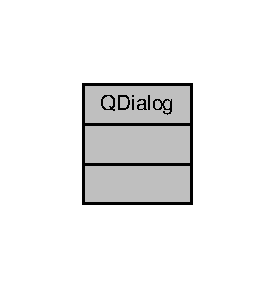
\includegraphics[width=132pt]{class_q_dialog__coll__graph}
\end{center}
\end{figure}


La documentation de cette classe a été générée à partir du fichier suivant \+:\begin{DoxyCompactItemize}
\item 
\hyperlink{reglages_alertes_ihm_8h}{reglages\+Alertes\+Ihm.\+h}\end{DoxyCompactItemize}

\hypertarget{class_q_object}{}\subsection{Référence de la classe Q\+Object}
\label{class_q_object}\index{Q\+Object@{Q\+Object}}


Graphe de collaboration de Q\+Object\+:\nopagebreak
\begin{figure}[H]
\begin{center}
\leavevmode
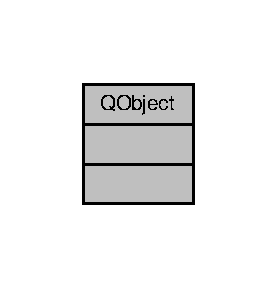
\includegraphics[width=133pt]{class_q_object__coll__graph}
\end{center}
\end{figure}


La documentation de cette classe a été générée à partir du fichier suivant \+:\begin{DoxyCompactItemize}
\item 
\hyperlink{infos_poids_8h}{infos\+Poids.\+h}\end{DoxyCompactItemize}

\hypertarget{class_q_widget}{}\subsection{Référence de la classe Q\+Widget}
\label{class_q_widget}\index{Q\+Widget@{Q\+Widget}}


Graphe de collaboration de Q\+Widget\+:\nopagebreak
\begin{figure}[H]
\begin{center}
\leavevmode
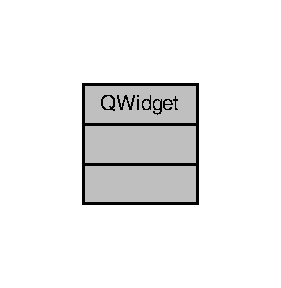
\includegraphics[width=135pt]{class_q_widget__coll__graph}
\end{center}
\end{figure}


La documentation de cette classe a été générée à partir du fichier suivant \+:\begin{DoxyCompactItemize}
\item 
\hyperlink{ruche_ihm_8h}{ruche\+Ihm.\+h}\end{DoxyCompactItemize}

\hypertarget{class_reglages_alertes_ihm}{}\subsection{Référence de la classe Reglages\+Alertes\+Ihm}
\label{class_reglages_alertes_ihm}\index{Reglages\+Alertes\+Ihm@{Reglages\+Alertes\+Ihm}}


Déclaration de la classe \hyperlink{class_reglages_alertes_ihm}{Reglages\+Alertes\+Ihm}.  




{\ttfamily \#include $<$reglages\+Alertes\+Ihm.\+h$>$}



Graphe de collaboration de Reglages\+Alertes\+Ihm\+:\nopagebreak
\begin{figure}[H]
\begin{center}
\leavevmode
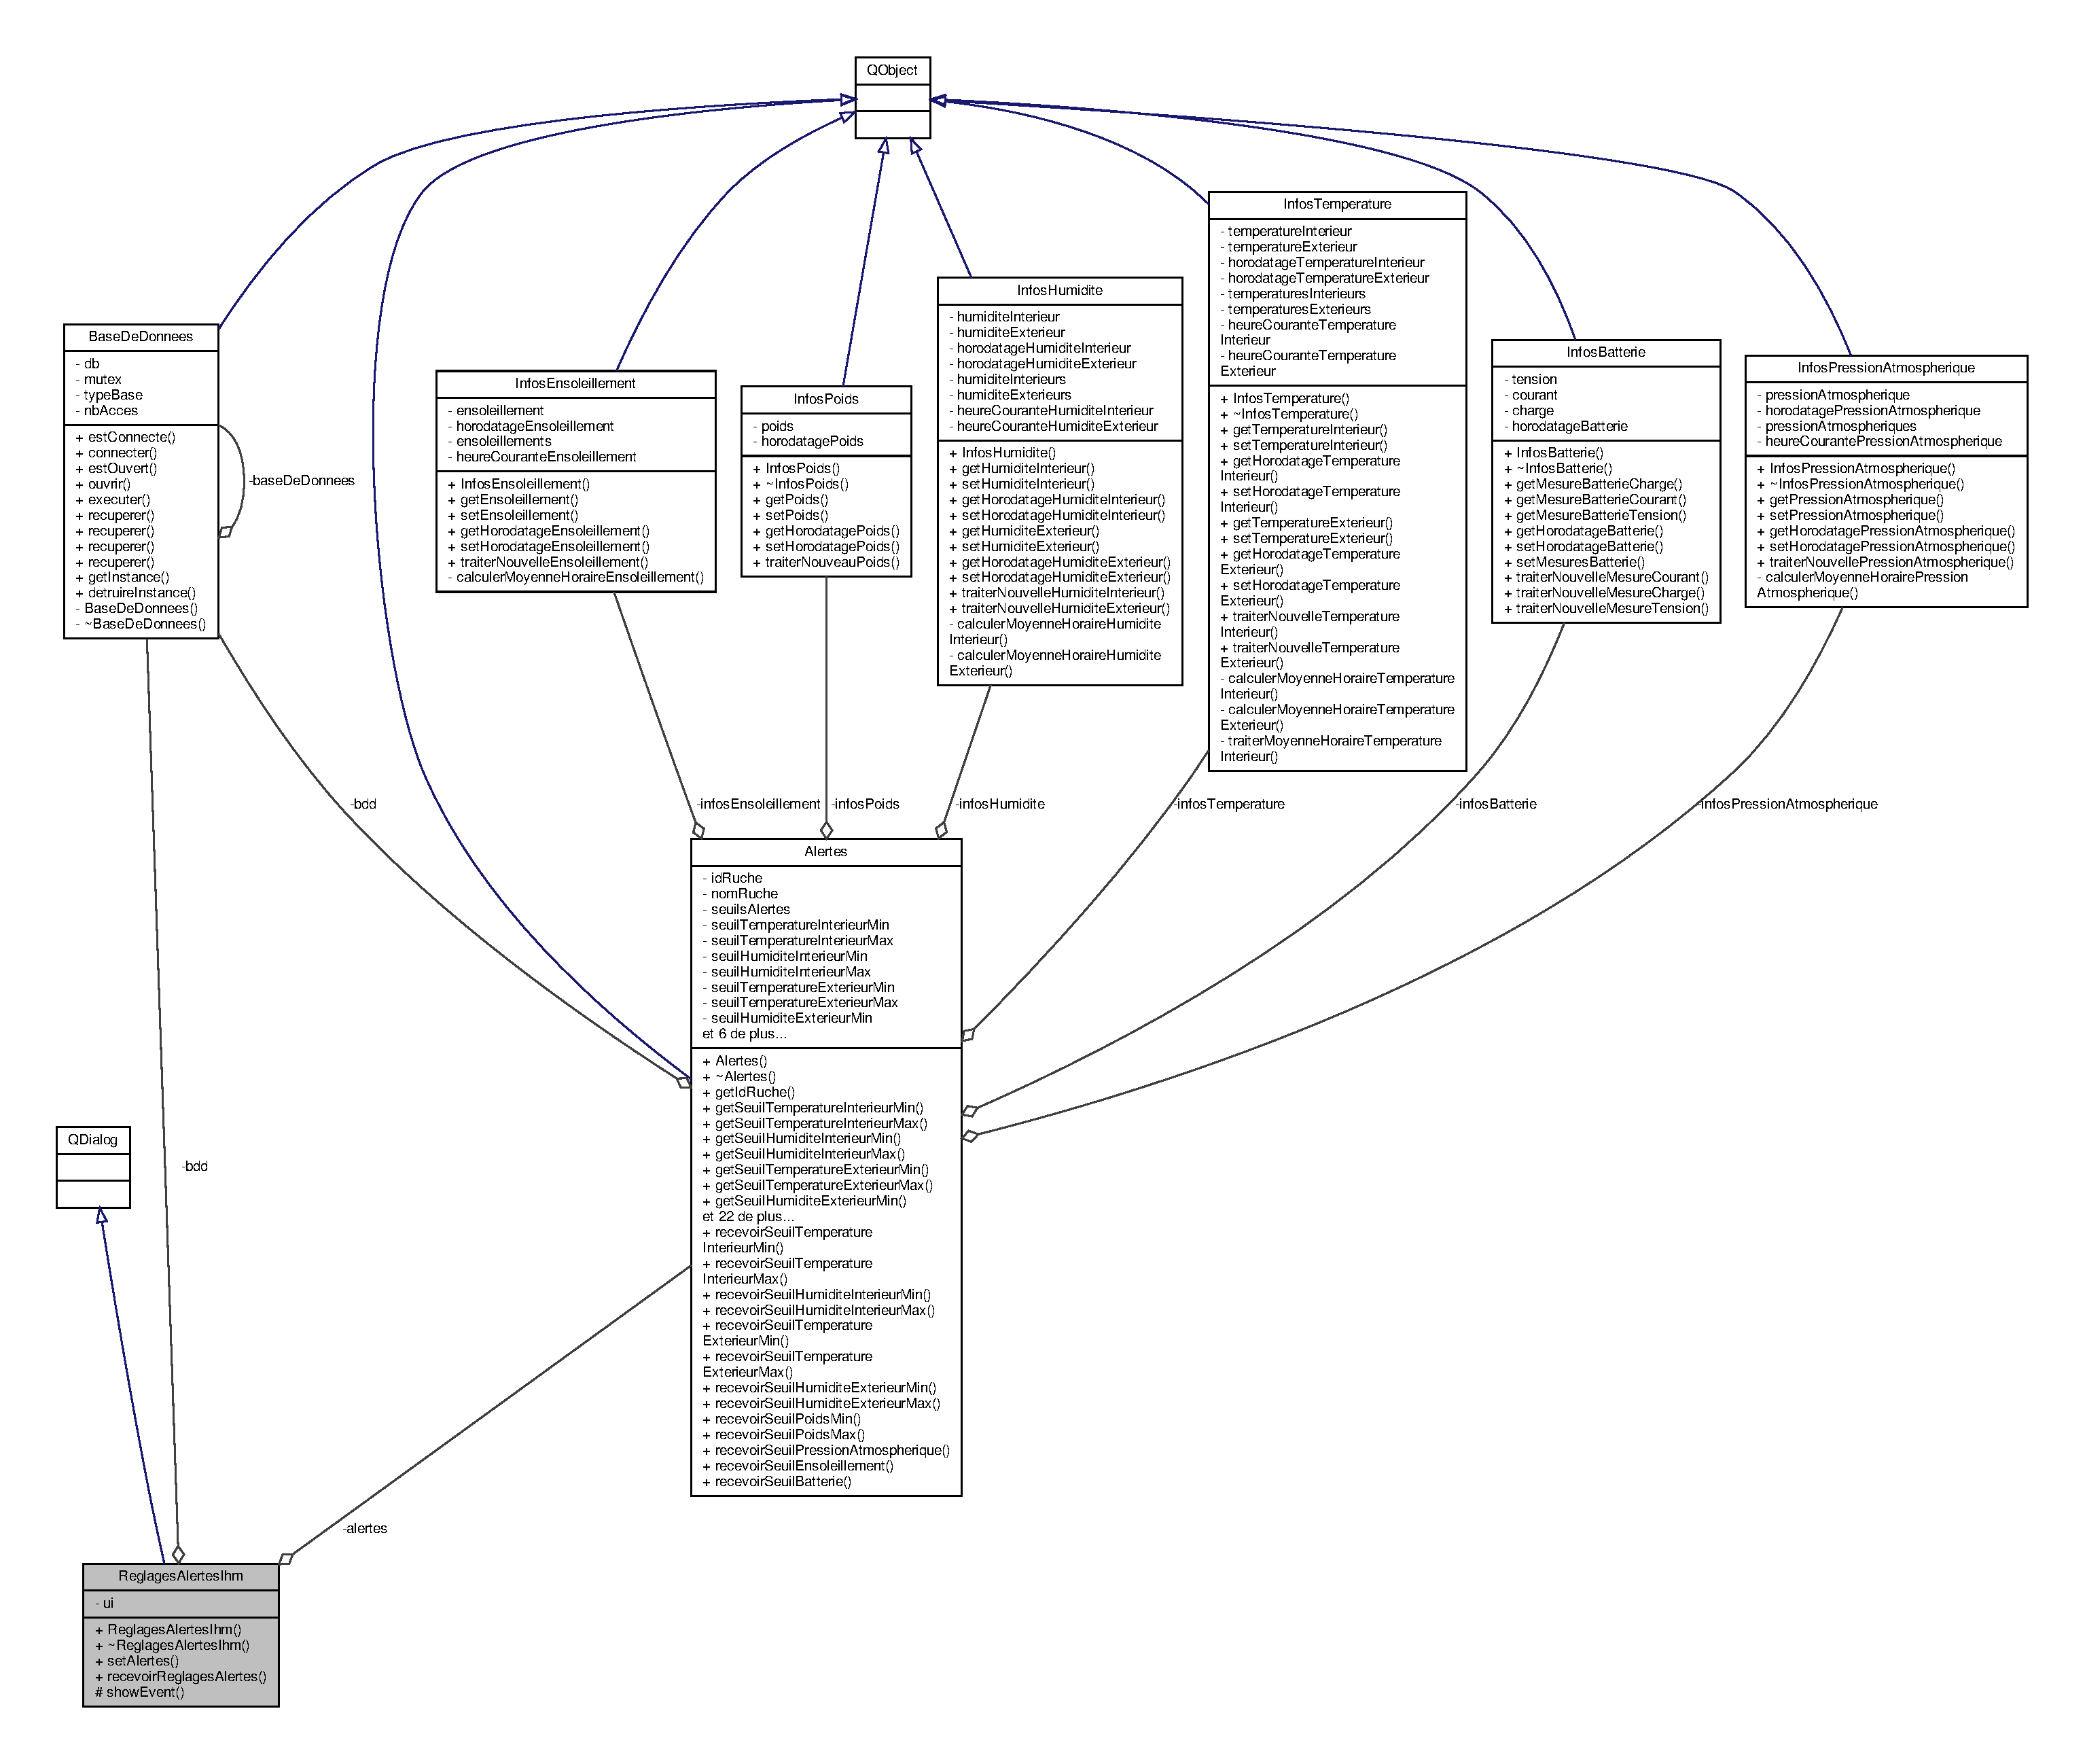
\includegraphics[width=350pt]{class_reglages_alertes_ihm__coll__graph}
\end{center}
\end{figure}
\subsubsection*{Connecteurs publics}
\begin{DoxyCompactItemize}
\item 
void \hyperlink{class_reglages_alertes_ihm_a5c40f718b28b948a90574ef0c2d3e587}{recevoir\+Reglages\+Alertes} ()
\begin{DoxyCompactList}\small\item\em recoit les paramétres de l\textquotesingle{}ihm \end{DoxyCompactList}\end{DoxyCompactItemize}
\subsubsection*{Signaux}
\begin{DoxyCompactItemize}
\item 
void \hyperlink{class_reglages_alertes_ihm_a44b51f5bfba7a28ee82b5e08d042c153}{envoi\+Seuil\+Temperature\+Interieur\+Min} (Q\+String seuil)
\item 
void \hyperlink{class_reglages_alertes_ihm_aa2695b931056a81e6e33ae5e9867b872}{envoi\+Seuil\+Temperature\+Interieur\+Max} (Q\+String seuil)
\item 
void \hyperlink{class_reglages_alertes_ihm_a0d913b26dd22ce48aaebed82a0d3df62}{envoi\+Seuil\+Humidite\+Interieur\+Min} (Q\+String seuil)
\item 
void \hyperlink{class_reglages_alertes_ihm_ae5e409ea2353cc8e43f312e252b365f9}{envoi\+Seuil\+Humidite\+Interieur\+Max} (Q\+String seuil)
\item 
void \hyperlink{class_reglages_alertes_ihm_a5c4cadb3f7a76cecc0bafaa297b2898a}{envoi\+Seuil\+Temperature\+Exterieur\+Min} (Q\+String seuil)
\item 
void \hyperlink{class_reglages_alertes_ihm_a626e1067d882bb5c0b86c8e0fb063dcc}{envoi\+Seuil\+Temperature\+Exterieur\+Max} (Q\+String seuil)
\item 
void \hyperlink{class_reglages_alertes_ihm_a78cef50cbaaaa46c837230024129c092}{envoi\+Seuil\+Humidite\+Exterieur\+Min} (Q\+String seuil)
\item 
void \hyperlink{class_reglages_alertes_ihm_a1455ae71d0e6c33b7857a23d116f3248}{envoi\+Seuil\+Humidite\+Exterieur\+Max} (Q\+String seuil)
\item 
void \hyperlink{class_reglages_alertes_ihm_a1ff9b472f2eed0efece54da863497324}{envoi\+Seuil\+Ensoleillement\+Min} (Q\+String seuil)
\item 
void \hyperlink{class_reglages_alertes_ihm_a78ea60b683ff8bde49d8bd332eb71c57}{envoi\+Seuil\+Pression\+Atmospherique\+Min} (Q\+String seuil)
\item 
void \hyperlink{class_reglages_alertes_ihm_a6d4642c0f64bad9f070ce7988549f8df}{envoi\+Seuil\+Poids\+Min} (Q\+String seuil)
\item 
void \hyperlink{class_reglages_alertes_ihm_a60d8e26bf08448029f4592b10297bdd1}{envoi\+Seuil\+Poids\+Max} (Q\+String seuil)
\end{DoxyCompactItemize}
\subsubsection*{Fonctions membres publiques}
\begin{DoxyCompactItemize}
\item 
\hyperlink{class_reglages_alertes_ihm_ae6337f2d05a3184e48bf5022a91f06c7}{Reglages\+Alertes\+Ihm} (\hyperlink{class_q_widget}{Q\+Widget} $\ast$parent=0)
\begin{DoxyCompactList}\small\item\em Constructeur de la fenêtre principale. \end{DoxyCompactList}\item 
\hyperlink{class_reglages_alertes_ihm_aa9bfc09b4162f536de84d218daa36982}{$\sim$\+Reglages\+Alertes\+Ihm} ()
\begin{DoxyCompactList}\small\item\em Destructeur de la fenêtre principale. \end{DoxyCompactList}\item 
void \hyperlink{class_reglages_alertes_ihm_aeb0331a6103f944cb15cdd62985ca231}{set\+Alertes} (\hyperlink{class_alertes}{Alertes} $\ast$\hyperlink{class_reglages_alertes_ihm_a9afa97e737d3c6a9a28a23fc4bc4beeb}{alertes})
\begin{DoxyCompactList}\small\item\em setter de l\textquotesingle{}objet alertes \end{DoxyCompactList}\end{DoxyCompactItemize}
\subsubsection*{Fonctions membres protégées}
\begin{DoxyCompactItemize}
\item 
void \hyperlink{class_reglages_alertes_ihm_af47504b34ab0213fce9269c08b9e5544}{show\+Event} (Q\+Show\+Event $\ast$ev)
\begin{DoxyCompactList}\small\item\em affiche les seuils à chaque fois que la fenêtre sera affichée \end{DoxyCompactList}\end{DoxyCompactItemize}
\subsubsection*{Attributs privés}
\begin{DoxyCompactItemize}
\item 
Ui\+::\+Reglages\+Alertes\+Ihm $\ast$ \hyperlink{class_reglages_alertes_ihm_af3a1fcc84fb1c76248b330372947b245}{ui}
\item 
\hyperlink{class_alertes}{Alertes} $\ast$ \hyperlink{class_reglages_alertes_ihm_a9afa97e737d3c6a9a28a23fc4bc4beeb}{alertes}
\item 
\hyperlink{class_base_de_donnees}{Base\+De\+Donnees} $\ast$ \hyperlink{class_reglages_alertes_ihm_a91b511776c98009cf8f951ec9f3e564e}{bdd}
\begin{DoxyCompactList}\small\item\em agrégation de l\textquotesingle{}objet \hyperlink{class_base_de_donnees}{Base\+De\+Donnees} \end{DoxyCompactList}\end{DoxyCompactItemize}


\subsubsection{Description détaillée}
\begin{DoxyAuthor}{Auteur}
Florentin Mellah, Enzo Rossi
\end{DoxyAuthor}
\begin{DoxyVersion}{Version}
1.\+1 
\end{DoxyVersion}


\subsubsection{Documentation des constructeurs et destructeur}
\mbox{\Hypertarget{class_reglages_alertes_ihm_ae6337f2d05a3184e48bf5022a91f06c7}\label{class_reglages_alertes_ihm_ae6337f2d05a3184e48bf5022a91f06c7}} 
\index{Reglages\+Alertes\+Ihm@{Reglages\+Alertes\+Ihm}!Reglages\+Alertes\+Ihm@{Reglages\+Alertes\+Ihm}}
\index{Reglages\+Alertes\+Ihm@{Reglages\+Alertes\+Ihm}!Reglages\+Alertes\+Ihm@{Reglages\+Alertes\+Ihm}}
\paragraph{\texorpdfstring{Reglages\+Alertes\+Ihm()}{ReglagesAlertesIhm()}}
{\footnotesize\ttfamily Reglages\+Alertes\+Ihm\+::\+Reglages\+Alertes\+Ihm (\begin{DoxyParamCaption}\item[{\hyperlink{class_q_widget}{Q\+Widget} $\ast$}]{parent = {\ttfamily 0} }\end{DoxyParamCaption})\hspace{0.3cm}{\ttfamily [explicit]}}


\begin{DoxyParams}{Paramètres}
{\em parent} & \hyperlink{class_q_object}{Q\+Object} Adresse de l\textquotesingle{}objet Qt parent (0 = fenêtre principale) \\
\hline
\end{DoxyParams}


Références \hyperlink{class_reglages_alertes_ihm_a91b511776c98009cf8f951ec9f3e564e}{bdd}, \hyperlink{parametres_8h_a45f8f15b8f9a7ab4c2b219038ff64f6b}{B\+D\+D\+\_\+\+N\+O\+M\+B\+A\+SE}, \hyperlink{parametres_8h_ae2ded9166ed2553182545e97514c04f7}{B\+D\+D\+\_\+\+P\+A\+S\+S\+W\+O\+RD}, \hyperlink{parametres_8h_a423559dc987673b8aacaa9f369839bb0}{B\+D\+D\+\_\+\+S\+E\+R\+V\+E\+UR}, \hyperlink{parametres_8h_a88b5f5b81fa534553c68802384beff2c}{B\+D\+D\+\_\+\+U\+S\+E\+R\+N\+A\+ME}, \hyperlink{class_base_de_donnees_ac20da193923a9bfea5e38ee5a54820cd}{Base\+De\+Donnees\+::connecter()}, \hyperlink{class_base_de_donnees_a00388973f3ec42e5c8e76e7af7e124b2}{Base\+De\+Donnees\+::est\+Connecte()}, \hyperlink{class_base_de_donnees_a80028aa2b6b4fbf30fb2e36357b7d3d3}{Base\+De\+Donnees\+::get\+Instance()}, \hyperlink{class_reglages_alertes_ihm_a5c40f718b28b948a90574ef0c2d3e587}{recevoir\+Reglages\+Alertes()}, et \hyperlink{class_reglages_alertes_ihm_af3a1fcc84fb1c76248b330372947b245}{ui}.


\begin{DoxyCode}
00025                                                       :
00026     \hyperlink{class_q_dialog}{QDialog}(parent),
00027     \hyperlink{class_reglages_alertes_ihm_af3a1fcc84fb1c76248b330372947b245}{ui}(\textcolor{keyword}{new} Ui::ReglagesAlertesIhm), \hyperlink{class_reglages_alertes_ihm_a9afa97e737d3c6a9a28a23fc4bc4beeb}{alertes}(0)
00028 \{
00029     \hyperlink{class_reglages_alertes_ihm_af3a1fcc84fb1c76248b330372947b245}{ui}->setupUi(\textcolor{keyword}{this});
00030 
00031     \hyperlink{class_reglages_alertes_ihm_a91b511776c98009cf8f951ec9f3e564e}{bdd} = \hyperlink{class_base_de_donnees_a80028aa2b6b4fbf30fb2e36357b7d3d3}{BaseDeDonnees::getInstance}();
00032     \textcolor{keywordflow}{if}(!\hyperlink{class_reglages_alertes_ihm_a91b511776c98009cf8f951ec9f3e564e}{bdd}->\hyperlink{class_base_de_donnees_a00388973f3ec42e5c8e76e7af7e124b2}{estConnecte}())
00033         \hyperlink{class_reglages_alertes_ihm_a91b511776c98009cf8f951ec9f3e564e}{bdd}->\hyperlink{class_base_de_donnees_ac20da193923a9bfea5e38ee5a54820cd}{connecter}(\hyperlink{parametres_8h_a45f8f15b8f9a7ab4c2b219038ff64f6b}{BDD\_NOMBASE}, \hyperlink{parametres_8h_a88b5f5b81fa534553c68802384beff2c}{BDD\_USERNAME}, 
      \hyperlink{parametres_8h_ae2ded9166ed2553182545e97514c04f7}{BDD\_PASSWORD}, \hyperlink{parametres_8h_a423559dc987673b8aacaa9f369839bb0}{BDD\_SERVEUR});
00034 
00035     connect(\hyperlink{class_reglages_alertes_ihm_af3a1fcc84fb1c76248b330372947b245}{ui}->pushButtonOk,SIGNAL(clicked(\textcolor{keywordtype}{bool})),\textcolor{keyword}{this},SLOT(accept()));
00036     connect(\hyperlink{class_reglages_alertes_ihm_af3a1fcc84fb1c76248b330372947b245}{ui}->pushButtonOk,SIGNAL(clicked(\textcolor{keywordtype}{bool})),\textcolor{keyword}{this} ,SLOT(
      \hyperlink{class_reglages_alertes_ihm_a5c40f718b28b948a90574ef0c2d3e587}{recevoirReglagesAlertes}()));
00037 \}
\end{DoxyCode}
\mbox{\Hypertarget{class_reglages_alertes_ihm_aa9bfc09b4162f536de84d218daa36982}\label{class_reglages_alertes_ihm_aa9bfc09b4162f536de84d218daa36982}} 
\index{Reglages\+Alertes\+Ihm@{Reglages\+Alertes\+Ihm}!````~Reglages\+Alertes\+Ihm@{$\sim$\+Reglages\+Alertes\+Ihm}}
\index{````~Reglages\+Alertes\+Ihm@{$\sim$\+Reglages\+Alertes\+Ihm}!Reglages\+Alertes\+Ihm@{Reglages\+Alertes\+Ihm}}
\paragraph{\texorpdfstring{$\sim$\+Reglages\+Alertes\+Ihm()}{~ReglagesAlertesIhm()}}
{\footnotesize\ttfamily Reglages\+Alertes\+Ihm\+::$\sim$\+Reglages\+Alertes\+Ihm (\begin{DoxyParamCaption}{ }\end{DoxyParamCaption})}



Références \hyperlink{class_base_de_donnees_a457401c0816b888c77ce915997545f4e}{Base\+De\+Donnees\+::detruire\+Instance()}, et \hyperlink{class_reglages_alertes_ihm_af3a1fcc84fb1c76248b330372947b245}{ui}.


\begin{DoxyCode}
00046 \{
00047     \textcolor{keyword}{delete} \hyperlink{class_reglages_alertes_ihm_af3a1fcc84fb1c76248b330372947b245}{ui};
00048     \hyperlink{class_base_de_donnees_a457401c0816b888c77ce915997545f4e}{BaseDeDonnees::detruireInstance}();
00049 \}
\end{DoxyCode}


\subsubsection{Documentation des fonctions membres}
\mbox{\Hypertarget{class_reglages_alertes_ihm_a1ff9b472f2eed0efece54da863497324}\label{class_reglages_alertes_ihm_a1ff9b472f2eed0efece54da863497324}} 
\index{Reglages\+Alertes\+Ihm@{Reglages\+Alertes\+Ihm}!envoi\+Seuil\+Ensoleillement\+Min@{envoi\+Seuil\+Ensoleillement\+Min}}
\index{envoi\+Seuil\+Ensoleillement\+Min@{envoi\+Seuil\+Ensoleillement\+Min}!Reglages\+Alertes\+Ihm@{Reglages\+Alertes\+Ihm}}
\paragraph{\texorpdfstring{envoi\+Seuil\+Ensoleillement\+Min}{envoiSeuilEnsoleillementMin}}
{\footnotesize\ttfamily void Reglages\+Alertes\+Ihm\+::envoi\+Seuil\+Ensoleillement\+Min (\begin{DoxyParamCaption}\item[{Q\+String}]{seuil }\end{DoxyParamCaption})\hspace{0.3cm}{\ttfamily [signal]}}



Référencé par \hyperlink{class_reglages_alertes_ihm_a5c40f718b28b948a90574ef0c2d3e587}{recevoir\+Reglages\+Alertes()}, et \hyperlink{class_reglages_alertes_ihm_aeb0331a6103f944cb15cdd62985ca231}{set\+Alertes()}.

\mbox{\Hypertarget{class_reglages_alertes_ihm_a1455ae71d0e6c33b7857a23d116f3248}\label{class_reglages_alertes_ihm_a1455ae71d0e6c33b7857a23d116f3248}} 
\index{Reglages\+Alertes\+Ihm@{Reglages\+Alertes\+Ihm}!envoi\+Seuil\+Humidite\+Exterieur\+Max@{envoi\+Seuil\+Humidite\+Exterieur\+Max}}
\index{envoi\+Seuil\+Humidite\+Exterieur\+Max@{envoi\+Seuil\+Humidite\+Exterieur\+Max}!Reglages\+Alertes\+Ihm@{Reglages\+Alertes\+Ihm}}
\paragraph{\texorpdfstring{envoi\+Seuil\+Humidite\+Exterieur\+Max}{envoiSeuilHumiditeExterieurMax}}
{\footnotesize\ttfamily void Reglages\+Alertes\+Ihm\+::envoi\+Seuil\+Humidite\+Exterieur\+Max (\begin{DoxyParamCaption}\item[{Q\+String}]{seuil }\end{DoxyParamCaption})\hspace{0.3cm}{\ttfamily [signal]}}



Référencé par \hyperlink{class_reglages_alertes_ihm_a5c40f718b28b948a90574ef0c2d3e587}{recevoir\+Reglages\+Alertes()}, et \hyperlink{class_reglages_alertes_ihm_aeb0331a6103f944cb15cdd62985ca231}{set\+Alertes()}.

\mbox{\Hypertarget{class_reglages_alertes_ihm_a78cef50cbaaaa46c837230024129c092}\label{class_reglages_alertes_ihm_a78cef50cbaaaa46c837230024129c092}} 
\index{Reglages\+Alertes\+Ihm@{Reglages\+Alertes\+Ihm}!envoi\+Seuil\+Humidite\+Exterieur\+Min@{envoi\+Seuil\+Humidite\+Exterieur\+Min}}
\index{envoi\+Seuil\+Humidite\+Exterieur\+Min@{envoi\+Seuil\+Humidite\+Exterieur\+Min}!Reglages\+Alertes\+Ihm@{Reglages\+Alertes\+Ihm}}
\paragraph{\texorpdfstring{envoi\+Seuil\+Humidite\+Exterieur\+Min}{envoiSeuilHumiditeExterieurMin}}
{\footnotesize\ttfamily void Reglages\+Alertes\+Ihm\+::envoi\+Seuil\+Humidite\+Exterieur\+Min (\begin{DoxyParamCaption}\item[{Q\+String}]{seuil }\end{DoxyParamCaption})\hspace{0.3cm}{\ttfamily [signal]}}



Référencé par \hyperlink{class_reglages_alertes_ihm_a5c40f718b28b948a90574ef0c2d3e587}{recevoir\+Reglages\+Alertes()}, et \hyperlink{class_reglages_alertes_ihm_aeb0331a6103f944cb15cdd62985ca231}{set\+Alertes()}.

\mbox{\Hypertarget{class_reglages_alertes_ihm_ae5e409ea2353cc8e43f312e252b365f9}\label{class_reglages_alertes_ihm_ae5e409ea2353cc8e43f312e252b365f9}} 
\index{Reglages\+Alertes\+Ihm@{Reglages\+Alertes\+Ihm}!envoi\+Seuil\+Humidite\+Interieur\+Max@{envoi\+Seuil\+Humidite\+Interieur\+Max}}
\index{envoi\+Seuil\+Humidite\+Interieur\+Max@{envoi\+Seuil\+Humidite\+Interieur\+Max}!Reglages\+Alertes\+Ihm@{Reglages\+Alertes\+Ihm}}
\paragraph{\texorpdfstring{envoi\+Seuil\+Humidite\+Interieur\+Max}{envoiSeuilHumiditeInterieurMax}}
{\footnotesize\ttfamily void Reglages\+Alertes\+Ihm\+::envoi\+Seuil\+Humidite\+Interieur\+Max (\begin{DoxyParamCaption}\item[{Q\+String}]{seuil }\end{DoxyParamCaption})\hspace{0.3cm}{\ttfamily [signal]}}



Référencé par \hyperlink{class_reglages_alertes_ihm_a5c40f718b28b948a90574ef0c2d3e587}{recevoir\+Reglages\+Alertes()}, et \hyperlink{class_reglages_alertes_ihm_aeb0331a6103f944cb15cdd62985ca231}{set\+Alertes()}.

\mbox{\Hypertarget{class_reglages_alertes_ihm_a0d913b26dd22ce48aaebed82a0d3df62}\label{class_reglages_alertes_ihm_a0d913b26dd22ce48aaebed82a0d3df62}} 
\index{Reglages\+Alertes\+Ihm@{Reglages\+Alertes\+Ihm}!envoi\+Seuil\+Humidite\+Interieur\+Min@{envoi\+Seuil\+Humidite\+Interieur\+Min}}
\index{envoi\+Seuil\+Humidite\+Interieur\+Min@{envoi\+Seuil\+Humidite\+Interieur\+Min}!Reglages\+Alertes\+Ihm@{Reglages\+Alertes\+Ihm}}
\paragraph{\texorpdfstring{envoi\+Seuil\+Humidite\+Interieur\+Min}{envoiSeuilHumiditeInterieurMin}}
{\footnotesize\ttfamily void Reglages\+Alertes\+Ihm\+::envoi\+Seuil\+Humidite\+Interieur\+Min (\begin{DoxyParamCaption}\item[{Q\+String}]{seuil }\end{DoxyParamCaption})\hspace{0.3cm}{\ttfamily [signal]}}



Référencé par \hyperlink{class_reglages_alertes_ihm_a5c40f718b28b948a90574ef0c2d3e587}{recevoir\+Reglages\+Alertes()}, et \hyperlink{class_reglages_alertes_ihm_aeb0331a6103f944cb15cdd62985ca231}{set\+Alertes()}.

\mbox{\Hypertarget{class_reglages_alertes_ihm_a60d8e26bf08448029f4592b10297bdd1}\label{class_reglages_alertes_ihm_a60d8e26bf08448029f4592b10297bdd1}} 
\index{Reglages\+Alertes\+Ihm@{Reglages\+Alertes\+Ihm}!envoi\+Seuil\+Poids\+Max@{envoi\+Seuil\+Poids\+Max}}
\index{envoi\+Seuil\+Poids\+Max@{envoi\+Seuil\+Poids\+Max}!Reglages\+Alertes\+Ihm@{Reglages\+Alertes\+Ihm}}
\paragraph{\texorpdfstring{envoi\+Seuil\+Poids\+Max}{envoiSeuilPoidsMax}}
{\footnotesize\ttfamily void Reglages\+Alertes\+Ihm\+::envoi\+Seuil\+Poids\+Max (\begin{DoxyParamCaption}\item[{Q\+String}]{seuil }\end{DoxyParamCaption})\hspace{0.3cm}{\ttfamily [signal]}}



Référencé par \hyperlink{class_reglages_alertes_ihm_a5c40f718b28b948a90574ef0c2d3e587}{recevoir\+Reglages\+Alertes()}, et \hyperlink{class_reglages_alertes_ihm_aeb0331a6103f944cb15cdd62985ca231}{set\+Alertes()}.

\mbox{\Hypertarget{class_reglages_alertes_ihm_a6d4642c0f64bad9f070ce7988549f8df}\label{class_reglages_alertes_ihm_a6d4642c0f64bad9f070ce7988549f8df}} 
\index{Reglages\+Alertes\+Ihm@{Reglages\+Alertes\+Ihm}!envoi\+Seuil\+Poids\+Min@{envoi\+Seuil\+Poids\+Min}}
\index{envoi\+Seuil\+Poids\+Min@{envoi\+Seuil\+Poids\+Min}!Reglages\+Alertes\+Ihm@{Reglages\+Alertes\+Ihm}}
\paragraph{\texorpdfstring{envoi\+Seuil\+Poids\+Min}{envoiSeuilPoidsMin}}
{\footnotesize\ttfamily void Reglages\+Alertes\+Ihm\+::envoi\+Seuil\+Poids\+Min (\begin{DoxyParamCaption}\item[{Q\+String}]{seuil }\end{DoxyParamCaption})\hspace{0.3cm}{\ttfamily [signal]}}



Référencé par \hyperlink{class_reglages_alertes_ihm_a5c40f718b28b948a90574ef0c2d3e587}{recevoir\+Reglages\+Alertes()}, et \hyperlink{class_reglages_alertes_ihm_aeb0331a6103f944cb15cdd62985ca231}{set\+Alertes()}.

\mbox{\Hypertarget{class_reglages_alertes_ihm_a78ea60b683ff8bde49d8bd332eb71c57}\label{class_reglages_alertes_ihm_a78ea60b683ff8bde49d8bd332eb71c57}} 
\index{Reglages\+Alertes\+Ihm@{Reglages\+Alertes\+Ihm}!envoi\+Seuil\+Pression\+Atmospherique\+Min@{envoi\+Seuil\+Pression\+Atmospherique\+Min}}
\index{envoi\+Seuil\+Pression\+Atmospherique\+Min@{envoi\+Seuil\+Pression\+Atmospherique\+Min}!Reglages\+Alertes\+Ihm@{Reglages\+Alertes\+Ihm}}
\paragraph{\texorpdfstring{envoi\+Seuil\+Pression\+Atmospherique\+Min}{envoiSeuilPressionAtmospheriqueMin}}
{\footnotesize\ttfamily void Reglages\+Alertes\+Ihm\+::envoi\+Seuil\+Pression\+Atmospherique\+Min (\begin{DoxyParamCaption}\item[{Q\+String}]{seuil }\end{DoxyParamCaption})\hspace{0.3cm}{\ttfamily [signal]}}



Référencé par \hyperlink{class_reglages_alertes_ihm_a5c40f718b28b948a90574ef0c2d3e587}{recevoir\+Reglages\+Alertes()}, et \hyperlink{class_reglages_alertes_ihm_aeb0331a6103f944cb15cdd62985ca231}{set\+Alertes()}.

\mbox{\Hypertarget{class_reglages_alertes_ihm_a626e1067d882bb5c0b86c8e0fb063dcc}\label{class_reglages_alertes_ihm_a626e1067d882bb5c0b86c8e0fb063dcc}} 
\index{Reglages\+Alertes\+Ihm@{Reglages\+Alertes\+Ihm}!envoi\+Seuil\+Temperature\+Exterieur\+Max@{envoi\+Seuil\+Temperature\+Exterieur\+Max}}
\index{envoi\+Seuil\+Temperature\+Exterieur\+Max@{envoi\+Seuil\+Temperature\+Exterieur\+Max}!Reglages\+Alertes\+Ihm@{Reglages\+Alertes\+Ihm}}
\paragraph{\texorpdfstring{envoi\+Seuil\+Temperature\+Exterieur\+Max}{envoiSeuilTemperatureExterieurMax}}
{\footnotesize\ttfamily void Reglages\+Alertes\+Ihm\+::envoi\+Seuil\+Temperature\+Exterieur\+Max (\begin{DoxyParamCaption}\item[{Q\+String}]{seuil }\end{DoxyParamCaption})\hspace{0.3cm}{\ttfamily [signal]}}



Référencé par \hyperlink{class_reglages_alertes_ihm_a5c40f718b28b948a90574ef0c2d3e587}{recevoir\+Reglages\+Alertes()}, et \hyperlink{class_reglages_alertes_ihm_aeb0331a6103f944cb15cdd62985ca231}{set\+Alertes()}.

\mbox{\Hypertarget{class_reglages_alertes_ihm_a5c4cadb3f7a76cecc0bafaa297b2898a}\label{class_reglages_alertes_ihm_a5c4cadb3f7a76cecc0bafaa297b2898a}} 
\index{Reglages\+Alertes\+Ihm@{Reglages\+Alertes\+Ihm}!envoi\+Seuil\+Temperature\+Exterieur\+Min@{envoi\+Seuil\+Temperature\+Exterieur\+Min}}
\index{envoi\+Seuil\+Temperature\+Exterieur\+Min@{envoi\+Seuil\+Temperature\+Exterieur\+Min}!Reglages\+Alertes\+Ihm@{Reglages\+Alertes\+Ihm}}
\paragraph{\texorpdfstring{envoi\+Seuil\+Temperature\+Exterieur\+Min}{envoiSeuilTemperatureExterieurMin}}
{\footnotesize\ttfamily void Reglages\+Alertes\+Ihm\+::envoi\+Seuil\+Temperature\+Exterieur\+Min (\begin{DoxyParamCaption}\item[{Q\+String}]{seuil }\end{DoxyParamCaption})\hspace{0.3cm}{\ttfamily [signal]}}



Référencé par \hyperlink{class_reglages_alertes_ihm_a5c40f718b28b948a90574ef0c2d3e587}{recevoir\+Reglages\+Alertes()}, et \hyperlink{class_reglages_alertes_ihm_aeb0331a6103f944cb15cdd62985ca231}{set\+Alertes()}.

\mbox{\Hypertarget{class_reglages_alertes_ihm_aa2695b931056a81e6e33ae5e9867b872}\label{class_reglages_alertes_ihm_aa2695b931056a81e6e33ae5e9867b872}} 
\index{Reglages\+Alertes\+Ihm@{Reglages\+Alertes\+Ihm}!envoi\+Seuil\+Temperature\+Interieur\+Max@{envoi\+Seuil\+Temperature\+Interieur\+Max}}
\index{envoi\+Seuil\+Temperature\+Interieur\+Max@{envoi\+Seuil\+Temperature\+Interieur\+Max}!Reglages\+Alertes\+Ihm@{Reglages\+Alertes\+Ihm}}
\paragraph{\texorpdfstring{envoi\+Seuil\+Temperature\+Interieur\+Max}{envoiSeuilTemperatureInterieurMax}}
{\footnotesize\ttfamily void Reglages\+Alertes\+Ihm\+::envoi\+Seuil\+Temperature\+Interieur\+Max (\begin{DoxyParamCaption}\item[{Q\+String}]{seuil }\end{DoxyParamCaption})\hspace{0.3cm}{\ttfamily [signal]}}



Référencé par \hyperlink{class_reglages_alertes_ihm_a5c40f718b28b948a90574ef0c2d3e587}{recevoir\+Reglages\+Alertes()}, et \hyperlink{class_reglages_alertes_ihm_aeb0331a6103f944cb15cdd62985ca231}{set\+Alertes()}.

\mbox{\Hypertarget{class_reglages_alertes_ihm_a44b51f5bfba7a28ee82b5e08d042c153}\label{class_reglages_alertes_ihm_a44b51f5bfba7a28ee82b5e08d042c153}} 
\index{Reglages\+Alertes\+Ihm@{Reglages\+Alertes\+Ihm}!envoi\+Seuil\+Temperature\+Interieur\+Min@{envoi\+Seuil\+Temperature\+Interieur\+Min}}
\index{envoi\+Seuil\+Temperature\+Interieur\+Min@{envoi\+Seuil\+Temperature\+Interieur\+Min}!Reglages\+Alertes\+Ihm@{Reglages\+Alertes\+Ihm}}
\paragraph{\texorpdfstring{envoi\+Seuil\+Temperature\+Interieur\+Min}{envoiSeuilTemperatureInterieurMin}}
{\footnotesize\ttfamily void Reglages\+Alertes\+Ihm\+::envoi\+Seuil\+Temperature\+Interieur\+Min (\begin{DoxyParamCaption}\item[{Q\+String}]{seuil }\end{DoxyParamCaption})\hspace{0.3cm}{\ttfamily [signal]}}



Référencé par \hyperlink{class_reglages_alertes_ihm_a5c40f718b28b948a90574ef0c2d3e587}{recevoir\+Reglages\+Alertes()}, et \hyperlink{class_reglages_alertes_ihm_aeb0331a6103f944cb15cdd62985ca231}{set\+Alertes()}.

\mbox{\Hypertarget{class_reglages_alertes_ihm_a5c40f718b28b948a90574ef0c2d3e587}\label{class_reglages_alertes_ihm_a5c40f718b28b948a90574ef0c2d3e587}} 
\index{Reglages\+Alertes\+Ihm@{Reglages\+Alertes\+Ihm}!recevoir\+Reglages\+Alertes@{recevoir\+Reglages\+Alertes}}
\index{recevoir\+Reglages\+Alertes@{recevoir\+Reglages\+Alertes}!Reglages\+Alertes\+Ihm@{Reglages\+Alertes\+Ihm}}
\paragraph{\texorpdfstring{recevoir\+Reglages\+Alertes}{recevoirReglagesAlertes}}
{\footnotesize\ttfamily void Reglages\+Alertes\+Ihm\+::recevoir\+Reglages\+Alertes (\begin{DoxyParamCaption}{ }\end{DoxyParamCaption})\hspace{0.3cm}{\ttfamily [slot]}}



Références \hyperlink{class_reglages_alertes_ihm_a9afa97e737d3c6a9a28a23fc4bc4beeb}{alertes}, \hyperlink{class_reglages_alertes_ihm_a91b511776c98009cf8f951ec9f3e564e}{bdd}, \hyperlink{class_reglages_alertes_ihm_a1ff9b472f2eed0efece54da863497324}{envoi\+Seuil\+Ensoleillement\+Min()}, \hyperlink{class_reglages_alertes_ihm_a1455ae71d0e6c33b7857a23d116f3248}{envoi\+Seuil\+Humidite\+Exterieur\+Max()}, \hyperlink{class_reglages_alertes_ihm_a78cef50cbaaaa46c837230024129c092}{envoi\+Seuil\+Humidite\+Exterieur\+Min()}, \hyperlink{class_reglages_alertes_ihm_ae5e409ea2353cc8e43f312e252b365f9}{envoi\+Seuil\+Humidite\+Interieur\+Max()}, \hyperlink{class_reglages_alertes_ihm_a0d913b26dd22ce48aaebed82a0d3df62}{envoi\+Seuil\+Humidite\+Interieur\+Min()}, \hyperlink{class_reglages_alertes_ihm_a60d8e26bf08448029f4592b10297bdd1}{envoi\+Seuil\+Poids\+Max()}, \hyperlink{class_reglages_alertes_ihm_a6d4642c0f64bad9f070ce7988549f8df}{envoi\+Seuil\+Poids\+Min()}, \hyperlink{class_reglages_alertes_ihm_a78ea60b683ff8bde49d8bd332eb71c57}{envoi\+Seuil\+Pression\+Atmospherique\+Min()}, \hyperlink{class_reglages_alertes_ihm_a626e1067d882bb5c0b86c8e0fb063dcc}{envoi\+Seuil\+Temperature\+Exterieur\+Max()}, \hyperlink{class_reglages_alertes_ihm_a5c4cadb3f7a76cecc0bafaa297b2898a}{envoi\+Seuil\+Temperature\+Exterieur\+Min()}, \hyperlink{class_reglages_alertes_ihm_aa2695b931056a81e6e33ae5e9867b872}{envoi\+Seuil\+Temperature\+Interieur\+Max()}, \hyperlink{class_reglages_alertes_ihm_a44b51f5bfba7a28ee82b5e08d042c153}{envoi\+Seuil\+Temperature\+Interieur\+Min()}, \hyperlink{class_base_de_donnees_aa8de5f8f8bb17edc43f5c0ee33712081}{Base\+De\+Donnees\+::executer()}, \hyperlink{class_alertes_a2374f9e3e5dc95eacaa4eaa5d98540a7}{Alertes\+::get\+Id\+Ruche()}, \hyperlink{parametres_8h_a2d439ba3af9708601a7ae0edf3584d98}{P\+R\+E\+S\+S\+I\+O\+N\+\_\+\+A\+T\+M\+O\+S\+P\+H\+E\+R\+I\+Q\+U\+E\+\_\+\+S\+E\+U\+I\+L\+\_\+\+M\+AX}, et \hyperlink{class_reglages_alertes_ihm_af3a1fcc84fb1c76248b330372947b245}{ui}.



Référencé par \hyperlink{class_reglages_alertes_ihm_ae6337f2d05a3184e48bf5022a91f06c7}{Reglages\+Alertes\+Ihm()}.


\begin{DoxyCode}
00107 \{
00108     QString temperatureInterieurMin;
00109     QString temperatureInterieurMax;
00110     QString humiditeInterieurMin;
00111     QString humiditeInterieurMax;
00112     QString temperatureExterieurMin;
00113     QString temperatureExterieurMax;
00114     QString humiditeExterieurMin;
00115     QString humiditeExterieurMax;
00116     QString poidsMin;
00117     QString poidsMax;
00118     QString pressionAtmospheriqueMin;
00119     QString ensoleillementMin;
00120 
00121     temperatureInterieurMin = \hyperlink{class_reglages_alertes_ihm_af3a1fcc84fb1c76248b330372947b245}{ui}->lineEditSeuilTemperatureInterieurMin->text();
00122     temperatureInterieurMax= \hyperlink{class_reglages_alertes_ihm_af3a1fcc84fb1c76248b330372947b245}{ui}->lineEditSeuilTemperatureInterieurMax->text();
00123     humiditeInterieurMin = \hyperlink{class_reglages_alertes_ihm_af3a1fcc84fb1c76248b330372947b245}{ui}->lineEditSeuilHumiditeInterieurMin->text();
00124     humiditeInterieurMax = \hyperlink{class_reglages_alertes_ihm_af3a1fcc84fb1c76248b330372947b245}{ui}->lineEditSeuilHumiditeInterieurMax->text();
00125     temperatureExterieurMin = \hyperlink{class_reglages_alertes_ihm_af3a1fcc84fb1c76248b330372947b245}{ui}->lineEditSeuilTemperatureExterieurMin->text();
00126     temperatureExterieurMax = \hyperlink{class_reglages_alertes_ihm_af3a1fcc84fb1c76248b330372947b245}{ui}->lineEditSeuilTemperatureExterieurMax->text();
00127     humiditeExterieurMin = \hyperlink{class_reglages_alertes_ihm_af3a1fcc84fb1c76248b330372947b245}{ui}->lineEditSeuilHumiditeExterieurMin->text();
00128     humiditeExterieurMax = \hyperlink{class_reglages_alertes_ihm_af3a1fcc84fb1c76248b330372947b245}{ui}->lineEditSeuilHumiditeExterieurMax->text();
00129     poidsMin = \hyperlink{class_reglages_alertes_ihm_af3a1fcc84fb1c76248b330372947b245}{ui}->lineEditSeuilPoidsMin->text();
00130     poidsMax = \hyperlink{class_reglages_alertes_ihm_af3a1fcc84fb1c76248b330372947b245}{ui}->lineEditSeuilPoidsMax->text();
00131     pressionAtmospheriqueMin = \hyperlink{class_reglages_alertes_ihm_af3a1fcc84fb1c76248b330372947b245}{ui}->lineEditSeuilPressionAtmospherique->text();
00132     ensoleillementMin = \hyperlink{class_reglages_alertes_ihm_af3a1fcc84fb1c76248b330372947b245}{ui}->lineEditSeuilEnsoleillement->text();
00133 
00134     QString requete = \textcolor{stringliteral}{"UPDATE Seuils SET TemperatureIntMin='"} + temperatureInterieurMin + \textcolor{stringliteral}{"',
       TemperatureIntMax='"} + temperatureInterieurMax + \textcolor{stringliteral}{"', HumiditeIntMin='"} + humiditeInterieurMin + \textcolor{stringliteral}{"', HumiditeIntMax='"} + 
      humiditeInterieurMax + \textcolor{stringliteral}{"', TemperatureExtMin='"} + temperatureExterieurMin + \textcolor{stringliteral}{"', TemperatureExtMax='"} + 
      temperatureExterieurMax + \textcolor{stringliteral}{"', HumiditeExtMin='"} + humiditeExterieurMin + \textcolor{stringliteral}{"', HumiditeExtMax='"} + 
      humiditeExterieurMax +  \textcolor{stringliteral}{"', PressionMin='"} + pressionAtmospheriqueMin + \textcolor{stringliteral}{"', PressionMax='"} + QString::number(
      \hyperlink{parametres_8h_a2d439ba3af9708601a7ae0edf3584d98}{PRESSION\_ATMOSPHERIQUE\_SEUIL\_MAX}) + \textcolor{stringliteral}{"', PoidsMin='"} + poidsMin + \textcolor{stringliteral}{"',
       PoidsMax='"} + poidsMax + \textcolor{stringliteral}{"' WHERE idRuche='"} + this->\hyperlink{class_reglages_alertes_ihm_a9afa97e737d3c6a9a28a23fc4bc4beeb}{alertes}->\hyperlink{class_alertes_a2374f9e3e5dc95eacaa4eaa5d98540a7}{getIdRuche}() + \textcolor{stringliteral}{"'"};
00135     qDebug()<< Q\_FUNC\_INFO << requete;
00136     \textcolor{keywordtype}{bool} retour = \hyperlink{class_reglages_alertes_ihm_a91b511776c98009cf8f951ec9f3e564e}{bdd}->\hyperlink{class_base_de_donnees_aa8de5f8f8bb17edc43f5c0ee33712081}{executer}(requete);
00137     \textcolor{keywordflow}{if}(retour)
00138     \{
00139         qDebug() << Q\_FUNC\_INFO << temperatureInterieurMin;
00140         emit \hyperlink{class_reglages_alertes_ihm_a44b51f5bfba7a28ee82b5e08d042c153}{envoiSeuilTemperatureInterieurMin}(temperatureInterieurMin);
00141         emit \hyperlink{class_reglages_alertes_ihm_aa2695b931056a81e6e33ae5e9867b872}{envoiSeuilTemperatureInterieurMax}(temperatureInterieurMax);
00142         emit \hyperlink{class_reglages_alertes_ihm_a0d913b26dd22ce48aaebed82a0d3df62}{envoiSeuilHumiditeInterieurMin}(humiditeInterieurMin);
00143         emit \hyperlink{class_reglages_alertes_ihm_ae5e409ea2353cc8e43f312e252b365f9}{envoiSeuilHumiditeInterieurMax}(humiditeInterieurMax);
00144         emit \hyperlink{class_reglages_alertes_ihm_a5c4cadb3f7a76cecc0bafaa297b2898a}{envoiSeuilTemperatureExterieurMin}(temperatureExterieurMin);
00145         emit \hyperlink{class_reglages_alertes_ihm_a626e1067d882bb5c0b86c8e0fb063dcc}{envoiSeuilTemperatureExterieurMax}(temperatureExterieurMax);
00146         emit \hyperlink{class_reglages_alertes_ihm_a78cef50cbaaaa46c837230024129c092}{envoiSeuilHumiditeExterieurMin}(humiditeExterieurMin);
00147         emit \hyperlink{class_reglages_alertes_ihm_a1455ae71d0e6c33b7857a23d116f3248}{envoiSeuilHumiditeExterieurMax}(humiditeExterieurMax);
00148         emit \hyperlink{class_reglages_alertes_ihm_a6d4642c0f64bad9f070ce7988549f8df}{envoiSeuilPoidsMin}(poidsMin);
00149         emit \hyperlink{class_reglages_alertes_ihm_a60d8e26bf08448029f4592b10297bdd1}{envoiSeuilPoidsMax}(poidsMax);
00150         emit \hyperlink{class_reglages_alertes_ihm_a78ea60b683ff8bde49d8bd332eb71c57}{envoiSeuilPressionAtmospheriqueMin}(pressionAtmospheriqueMin)
      ;
00151         emit \hyperlink{class_reglages_alertes_ihm_a1ff9b472f2eed0efece54da863497324}{envoiSeuilEnsoleillementMin}(ensoleillementMin);
00152     \}
00153 \}
\end{DoxyCode}
\mbox{\Hypertarget{class_reglages_alertes_ihm_aeb0331a6103f944cb15cdd62985ca231}\label{class_reglages_alertes_ihm_aeb0331a6103f944cb15cdd62985ca231}} 
\index{Reglages\+Alertes\+Ihm@{Reglages\+Alertes\+Ihm}!set\+Alertes@{set\+Alertes}}
\index{set\+Alertes@{set\+Alertes}!Reglages\+Alertes\+Ihm@{Reglages\+Alertes\+Ihm}}
\paragraph{\texorpdfstring{set\+Alertes()}{setAlertes()}}
{\footnotesize\ttfamily void Reglages\+Alertes\+Ihm\+::set\+Alertes (\begin{DoxyParamCaption}\item[{\hyperlink{class_alertes}{Alertes} $\ast$}]{alertes }\end{DoxyParamCaption})}


\begin{DoxyParams}{Paramètres}
{\em $\ast$alertes} & correspond à l\textquotesingle{}objet de la classe \hyperlink{class_ruche_ihm}{Ruche\+Ihm} \\
\hline
\end{DoxyParams}


Références \hyperlink{class_reglages_alertes_ihm_a9afa97e737d3c6a9a28a23fc4bc4beeb}{alertes}, \hyperlink{class_reglages_alertes_ihm_a1ff9b472f2eed0efece54da863497324}{envoi\+Seuil\+Ensoleillement\+Min()}, \hyperlink{class_reglages_alertes_ihm_a1455ae71d0e6c33b7857a23d116f3248}{envoi\+Seuil\+Humidite\+Exterieur\+Max()}, \hyperlink{class_reglages_alertes_ihm_a78cef50cbaaaa46c837230024129c092}{envoi\+Seuil\+Humidite\+Exterieur\+Min()}, \hyperlink{class_reglages_alertes_ihm_ae5e409ea2353cc8e43f312e252b365f9}{envoi\+Seuil\+Humidite\+Interieur\+Max()}, \hyperlink{class_reglages_alertes_ihm_a0d913b26dd22ce48aaebed82a0d3df62}{envoi\+Seuil\+Humidite\+Interieur\+Min()}, \hyperlink{class_reglages_alertes_ihm_a60d8e26bf08448029f4592b10297bdd1}{envoi\+Seuil\+Poids\+Max()}, \hyperlink{class_reglages_alertes_ihm_a6d4642c0f64bad9f070ce7988549f8df}{envoi\+Seuil\+Poids\+Min()}, \hyperlink{class_reglages_alertes_ihm_a78ea60b683ff8bde49d8bd332eb71c57}{envoi\+Seuil\+Pression\+Atmospherique\+Min()}, \hyperlink{class_reglages_alertes_ihm_a626e1067d882bb5c0b86c8e0fb063dcc}{envoi\+Seuil\+Temperature\+Exterieur\+Max()}, \hyperlink{class_reglages_alertes_ihm_a5c4cadb3f7a76cecc0bafaa297b2898a}{envoi\+Seuil\+Temperature\+Exterieur\+Min()}, \hyperlink{class_reglages_alertes_ihm_aa2695b931056a81e6e33ae5e9867b872}{envoi\+Seuil\+Temperature\+Interieur\+Max()}, et \hyperlink{class_reglages_alertes_ihm_a44b51f5bfba7a28ee82b5e08d042c153}{envoi\+Seuil\+Temperature\+Interieur\+Min()}.



Référencé par \hyperlink{class_ruche_ihm_a7324ae6ea574ccdad47783f466933157}{Ruche\+Ihm\+::selectionner\+Ruche()}.


\begin{DoxyCode}
00057 \{
00058     \textcolor{keywordflow}{if}(this->alertes == 0)
00059     \{
00060         qDebug() << Q\_FUNC\_INFO << this->\hyperlink{class_reglages_alertes_ihm_a9afa97e737d3c6a9a28a23fc4bc4beeb}{alertes};
00061         this->alertes = \hyperlink{class_reglages_alertes_ihm_a9afa97e737d3c6a9a28a23fc4bc4beeb}{alertes};
00062         connect(\textcolor{keyword}{this}, SIGNAL(\hyperlink{class_reglages_alertes_ihm_a44b51f5bfba7a28ee82b5e08d042c153}{envoiSeuilTemperatureInterieurMin}(QString)), 
      this->alertes, SLOT(recevoirSeuilTemperatureInterieurMin(QString)));
00063         connect(\textcolor{keyword}{this}, SIGNAL(\hyperlink{class_reglages_alertes_ihm_aa2695b931056a81e6e33ae5e9867b872}{envoiSeuilTemperatureInterieurMax}(QString)), 
      this->alertes, SLOT(recevoirSeuilTemperatureInterieurMax(QString)));
00064         connect(\textcolor{keyword}{this}, SIGNAL(\hyperlink{class_reglages_alertes_ihm_a0d913b26dd22ce48aaebed82a0d3df62}{envoiSeuilHumiditeInterieurMin}(QString)), this->
      alertes, SLOT(recevoirSeuilHumiditeInterieurMin(QString)));
00065         connect(\textcolor{keyword}{this}, SIGNAL(\hyperlink{class_reglages_alertes_ihm_ae5e409ea2353cc8e43f312e252b365f9}{envoiSeuilHumiditeInterieurMax}(QString)), this->
      alertes, SLOT(recevoirSeuilHumiditeInterieurMax(QString)));
00066         connect(\textcolor{keyword}{this}, SIGNAL(\hyperlink{class_reglages_alertes_ihm_a5c4cadb3f7a76cecc0bafaa297b2898a}{envoiSeuilTemperatureExterieurMin}(QString)), 
      this->alertes, SLOT(recevoirSeuilTemperatureExterieurMin(QString)));
00067         connect(\textcolor{keyword}{this}, SIGNAL(\hyperlink{class_reglages_alertes_ihm_a626e1067d882bb5c0b86c8e0fb063dcc}{envoiSeuilTemperatureExterieurMax}(QString)), 
      this->alertes, SLOT(recevoirSeuilTemperatureExterieurMax(QString)));
00068         connect(\textcolor{keyword}{this}, SIGNAL(\hyperlink{class_reglages_alertes_ihm_a78cef50cbaaaa46c837230024129c092}{envoiSeuilHumiditeExterieurMin}(QString)), this->
      alertes, SLOT(recevoirSeuilHumiditeExterieurMin(QString)));
00069         connect(\textcolor{keyword}{this}, SIGNAL(\hyperlink{class_reglages_alertes_ihm_a1455ae71d0e6c33b7857a23d116f3248}{envoiSeuilHumiditeExterieurMax}(QString)), this->
      alertes, SLOT(recevoirSeuilHumiditeExterieurMax(QString)));
00070         connect(\textcolor{keyword}{this}, SIGNAL(\hyperlink{class_reglages_alertes_ihm_a6d4642c0f64bad9f070ce7988549f8df}{envoiSeuilPoidsMin}(QString)), this->alertes, SLOT(
      recevoirSeuilPoidsMin(QString)));
00071         connect(\textcolor{keyword}{this}, SIGNAL(\hyperlink{class_reglages_alertes_ihm_a60d8e26bf08448029f4592b10297bdd1}{envoiSeuilPoidsMax}(QString)), this->alertes, SLOT(
      recevoirSeuilPoidsMax(QString)));
00072         connect(\textcolor{keyword}{this}, SIGNAL(\hyperlink{class_reglages_alertes_ihm_a78ea60b683ff8bde49d8bd332eb71c57}{envoiSeuilPressionAtmospheriqueMin}(QString))
      , this->alertes, SLOT(recevoirSeuilPressionAtmospherique(QString)));
00073         connect(\textcolor{keyword}{this}, SIGNAL(\hyperlink{class_reglages_alertes_ihm_a1ff9b472f2eed0efece54da863497324}{envoiSeuilEnsoleillementMin}(QString)), this->
      alertes, SLOT(recevoirSeuilEnsoleillement(QString)));
00074     \}
00075 \}
\end{DoxyCode}
\mbox{\Hypertarget{class_reglages_alertes_ihm_af47504b34ab0213fce9269c08b9e5544}\label{class_reglages_alertes_ihm_af47504b34ab0213fce9269c08b9e5544}} 
\index{Reglages\+Alertes\+Ihm@{Reglages\+Alertes\+Ihm}!show\+Event@{show\+Event}}
\index{show\+Event@{show\+Event}!Reglages\+Alertes\+Ihm@{Reglages\+Alertes\+Ihm}}
\paragraph{\texorpdfstring{show\+Event()}{showEvent()}}
{\footnotesize\ttfamily void Reglages\+Alertes\+Ihm\+::show\+Event (\begin{DoxyParamCaption}\item[{Q\+Show\+Event $\ast$}]{ev }\end{DoxyParamCaption})\hspace{0.3cm}{\ttfamily [protected]}}


\begin{DoxyParams}{Paramètres}
{\em ev} & Q\+Show\+Event$\ast$ l\textquotesingle{}évènement \\
\hline
\end{DoxyParams}


Références \hyperlink{class_reglages_alertes_ihm_a9afa97e737d3c6a9a28a23fc4bc4beeb}{alertes}, \hyperlink{class_alertes_a54900058557979664d25137399ae2512}{Alertes\+::get\+Seuil\+Ensoleillement()}, \hyperlink{class_alertes_ad2c8daf5668f5d122efb9b84f7ea86de}{Alertes\+::get\+Seuil\+Humidite\+Exterieur\+Max()}, \hyperlink{class_alertes_a68e467e042b615f56347a0953d6e64f1}{Alertes\+::get\+Seuil\+Humidite\+Exterieur\+Min()}, \hyperlink{class_alertes_a86e0bb83ac1fa5e704e3b7b3fc7147cd}{Alertes\+::get\+Seuil\+Humidite\+Interieur\+Max()}, \hyperlink{class_alertes_a40d47b65952035b78cac05b915ad57b8}{Alertes\+::get\+Seuil\+Humidite\+Interieur\+Min()}, \hyperlink{class_alertes_a2c19b460f7f7cc7a867b5ed634371878}{Alertes\+::get\+Seuil\+Poids\+Max()}, \hyperlink{class_alertes_a228829e2826ee20cc014b2eb54addf14}{Alertes\+::get\+Seuil\+Poids\+Min()}, \hyperlink{class_alertes_a502fa36037246fb6eaad1db859bc1971}{Alertes\+::get\+Seuil\+Pression\+Atmospherique()}, \hyperlink{class_alertes_a00d834877e1fc34d7e0659ef6963ac4f}{Alertes\+::get\+Seuil\+Temperature\+Exterieur\+Max()}, \hyperlink{class_alertes_a4451c6b077256d838e584a073444d83d}{Alertes\+::get\+Seuil\+Temperature\+Exterieur\+Min()}, \hyperlink{class_alertes_ac514ebef5e7e65aa7bee0ebe3cd7e883}{Alertes\+::get\+Seuil\+Temperature\+Interieur\+Max()}, \hyperlink{class_alertes_af61b11556d97f923cf7dd25ac4f5dd05}{Alertes\+::get\+Seuil\+Temperature\+Interieur\+Min()}, et \hyperlink{class_reglages_alertes_ihm_af3a1fcc84fb1c76248b330372947b245}{ui}.


\begin{DoxyCode}
00083 \{
00084     Q\_UNUSED(ev)
00085     \textcolor{keywordflow}{if}(this->\hyperlink{class_reglages_alertes_ihm_a9afa97e737d3c6a9a28a23fc4bc4beeb}{alertes} != 0)
00086     \{
00087         \hyperlink{class_reglages_alertes_ihm_af3a1fcc84fb1c76248b330372947b245}{ui}->lineEditSeuilTemperatureInterieurMin->setText(QString::number(this->
      \hyperlink{class_reglages_alertes_ihm_a9afa97e737d3c6a9a28a23fc4bc4beeb}{alertes}->\hyperlink{class_alertes_af61b11556d97f923cf7dd25ac4f5dd05}{getSeuilTemperatureInterieurMin}()));
00088         \hyperlink{class_reglages_alertes_ihm_af3a1fcc84fb1c76248b330372947b245}{ui}->lineEditSeuilTemperatureInterieurMax->setText(QString::number(this->
      \hyperlink{class_reglages_alertes_ihm_a9afa97e737d3c6a9a28a23fc4bc4beeb}{alertes}->\hyperlink{class_alertes_ac514ebef5e7e65aa7bee0ebe3cd7e883}{getSeuilTemperatureInterieurMax}()));
00089         \hyperlink{class_reglages_alertes_ihm_af3a1fcc84fb1c76248b330372947b245}{ui}->lineEditSeuilHumiditeInterieurMin->setText(QString::number(this->
      \hyperlink{class_reglages_alertes_ihm_a9afa97e737d3c6a9a28a23fc4bc4beeb}{alertes}->\hyperlink{class_alertes_a40d47b65952035b78cac05b915ad57b8}{getSeuilHumiditeInterieurMin}()));
00090         \hyperlink{class_reglages_alertes_ihm_af3a1fcc84fb1c76248b330372947b245}{ui}->lineEditSeuilHumiditeInterieurMax->setText(QString::number(this->
      \hyperlink{class_reglages_alertes_ihm_a9afa97e737d3c6a9a28a23fc4bc4beeb}{alertes}->\hyperlink{class_alertes_a86e0bb83ac1fa5e704e3b7b3fc7147cd}{getSeuilHumiditeInterieurMax}()));
00091         \hyperlink{class_reglages_alertes_ihm_af3a1fcc84fb1c76248b330372947b245}{ui}->lineEditSeuilTemperatureExterieurMin->setText(QString::number(this->
      \hyperlink{class_reglages_alertes_ihm_a9afa97e737d3c6a9a28a23fc4bc4beeb}{alertes}->\hyperlink{class_alertes_a4451c6b077256d838e584a073444d83d}{getSeuilTemperatureExterieurMin}()));
00092         \hyperlink{class_reglages_alertes_ihm_af3a1fcc84fb1c76248b330372947b245}{ui}->lineEditSeuilTemperatureExterieurMax->setText(QString::number(this->
      \hyperlink{class_reglages_alertes_ihm_a9afa97e737d3c6a9a28a23fc4bc4beeb}{alertes}->\hyperlink{class_alertes_a00d834877e1fc34d7e0659ef6963ac4f}{getSeuilTemperatureExterieurMax}()));
00093         \hyperlink{class_reglages_alertes_ihm_af3a1fcc84fb1c76248b330372947b245}{ui}->lineEditSeuilHumiditeExterieurMin->setText(QString::number(this->
      \hyperlink{class_reglages_alertes_ihm_a9afa97e737d3c6a9a28a23fc4bc4beeb}{alertes}->\hyperlink{class_alertes_a68e467e042b615f56347a0953d6e64f1}{getSeuilHumiditeExterieurMin}()));
00094         \hyperlink{class_reglages_alertes_ihm_af3a1fcc84fb1c76248b330372947b245}{ui}->lineEditSeuilHumiditeExterieurMax->setText(QString::number(this->
      \hyperlink{class_reglages_alertes_ihm_a9afa97e737d3c6a9a28a23fc4bc4beeb}{alertes}->\hyperlink{class_alertes_ad2c8daf5668f5d122efb9b84f7ea86de}{getSeuilHumiditeExterieurMax}()));
00095         \hyperlink{class_reglages_alertes_ihm_af3a1fcc84fb1c76248b330372947b245}{ui}->lineEditSeuilPoidsMin->setText(QString::number(this->\hyperlink{class_reglages_alertes_ihm_a9afa97e737d3c6a9a28a23fc4bc4beeb}{alertes}->
      \hyperlink{class_alertes_a228829e2826ee20cc014b2eb54addf14}{getSeuilPoidsMin}()));
00096         \hyperlink{class_reglages_alertes_ihm_af3a1fcc84fb1c76248b330372947b245}{ui}->lineEditSeuilPoidsMax->setText(QString::number(this->\hyperlink{class_reglages_alertes_ihm_a9afa97e737d3c6a9a28a23fc4bc4beeb}{alertes}->
      \hyperlink{class_alertes_a2c19b460f7f7cc7a867b5ed634371878}{getSeuilPoidsMax}()));
00097         \hyperlink{class_reglages_alertes_ihm_af3a1fcc84fb1c76248b330372947b245}{ui}->lineEditSeuilPressionAtmospherique->setText(QString::number(this->
      \hyperlink{class_reglages_alertes_ihm_a9afa97e737d3c6a9a28a23fc4bc4beeb}{alertes}->\hyperlink{class_alertes_a502fa36037246fb6eaad1db859bc1971}{getSeuilPressionAtmospherique}()));
00098         \hyperlink{class_reglages_alertes_ihm_af3a1fcc84fb1c76248b330372947b245}{ui}->lineEditSeuilEnsoleillement->setText(QString::number(this->\hyperlink{class_reglages_alertes_ihm_a9afa97e737d3c6a9a28a23fc4bc4beeb}{alertes}->
      \hyperlink{class_alertes_a54900058557979664d25137399ae2512}{getSeuilEnsoleillement}()));
00099     \}
00100 \}
\end{DoxyCode}


\subsubsection{Documentation des données membres}
\mbox{\Hypertarget{class_reglages_alertes_ihm_a9afa97e737d3c6a9a28a23fc4bc4beeb}\label{class_reglages_alertes_ihm_a9afa97e737d3c6a9a28a23fc4bc4beeb}} 
\index{Reglages\+Alertes\+Ihm@{Reglages\+Alertes\+Ihm}!alertes@{alertes}}
\index{alertes@{alertes}!Reglages\+Alertes\+Ihm@{Reglages\+Alertes\+Ihm}}
\paragraph{\texorpdfstring{alertes}{alertes}}
{\footnotesize\ttfamily \hyperlink{class_alertes}{Alertes}$\ast$ Reglages\+Alertes\+Ihm\+::alertes\hspace{0.3cm}{\ttfamily [private]}}



Référencé par \hyperlink{class_reglages_alertes_ihm_a5c40f718b28b948a90574ef0c2d3e587}{recevoir\+Reglages\+Alertes()}, \hyperlink{class_reglages_alertes_ihm_aeb0331a6103f944cb15cdd62985ca231}{set\+Alertes()}, et \hyperlink{class_reglages_alertes_ihm_af47504b34ab0213fce9269c08b9e5544}{show\+Event()}.

\mbox{\Hypertarget{class_reglages_alertes_ihm_a91b511776c98009cf8f951ec9f3e564e}\label{class_reglages_alertes_ihm_a91b511776c98009cf8f951ec9f3e564e}} 
\index{Reglages\+Alertes\+Ihm@{Reglages\+Alertes\+Ihm}!bdd@{bdd}}
\index{bdd@{bdd}!Reglages\+Alertes\+Ihm@{Reglages\+Alertes\+Ihm}}
\paragraph{\texorpdfstring{bdd}{bdd}}
{\footnotesize\ttfamily \hyperlink{class_base_de_donnees}{Base\+De\+Donnees}$\ast$ Reglages\+Alertes\+Ihm\+::bdd\hspace{0.3cm}{\ttfamily [private]}}



Référencé par \hyperlink{class_reglages_alertes_ihm_a5c40f718b28b948a90574ef0c2d3e587}{recevoir\+Reglages\+Alertes()}, et \hyperlink{class_reglages_alertes_ihm_ae6337f2d05a3184e48bf5022a91f06c7}{Reglages\+Alertes\+Ihm()}.

\mbox{\Hypertarget{class_reglages_alertes_ihm_af3a1fcc84fb1c76248b330372947b245}\label{class_reglages_alertes_ihm_af3a1fcc84fb1c76248b330372947b245}} 
\index{Reglages\+Alertes\+Ihm@{Reglages\+Alertes\+Ihm}!ui@{ui}}
\index{ui@{ui}!Reglages\+Alertes\+Ihm@{Reglages\+Alertes\+Ihm}}
\paragraph{\texorpdfstring{ui}{ui}}
{\footnotesize\ttfamily Ui\+::\+Reglages\+Alertes\+Ihm$\ast$ Reglages\+Alertes\+Ihm\+::ui\hspace{0.3cm}{\ttfamily [private]}}



Référencé par \hyperlink{class_reglages_alertes_ihm_a5c40f718b28b948a90574ef0c2d3e587}{recevoir\+Reglages\+Alertes()}, \hyperlink{class_reglages_alertes_ihm_ae6337f2d05a3184e48bf5022a91f06c7}{Reglages\+Alertes\+Ihm()}, \hyperlink{class_reglages_alertes_ihm_af47504b34ab0213fce9269c08b9e5544}{show\+Event()}, et \hyperlink{class_reglages_alertes_ihm_aa9bfc09b4162f536de84d218daa36982}{$\sim$\+Reglages\+Alertes\+Ihm()}.



La documentation de cette classe a été générée à partir des fichiers suivants \+:\begin{DoxyCompactItemize}
\item 
\hyperlink{reglages_alertes_ihm_8h}{reglages\+Alertes\+Ihm.\+h}\item 
\hyperlink{reglages_alertes_ihm_8cpp}{reglages\+Alertes\+Ihm.\+cpp}\end{DoxyCompactItemize}

\hypertarget{classfr_1_1campus_1_1laurainc_1_1honeybee_1_1_ruche}{}\subsection{Référence de la classe fr.\+campus.\+laurainc.\+honeybee.\+Ruche}
\label{classfr_1_1campus_1_1laurainc_1_1honeybee_1_1_ruche}\index{fr.\+campus.\+laurainc.\+honeybee.\+Ruche@{fr.\+campus.\+laurainc.\+honeybee.\+Ruche}}


Graphe de collaboration de fr.\+campus.\+laurainc.\+honeybee.\+Ruche\+:\nopagebreak
\begin{figure}[H]
\begin{center}
\leavevmode
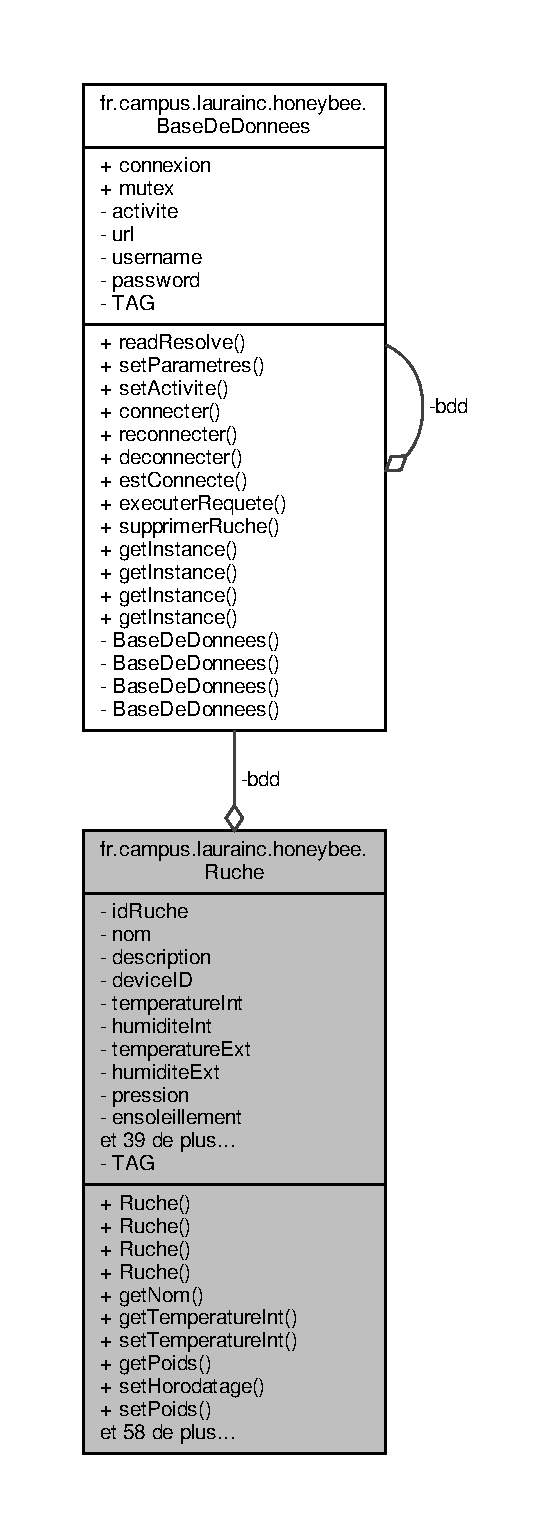
\includegraphics[height=550pt]{classfr_1_1campus_1_1laurainc_1_1honeybee_1_1_ruche__coll__graph}
\end{center}
\end{figure}
\subsubsection*{Fonctions membres publiques}
\begin{DoxyCompactItemize}
\item 
\hyperlink{classfr_1_1campus_1_1laurainc_1_1honeybee_1_1_ruche_a56ec53516e4f94b4f5e42f083fa345db}{Ruche} ()
\begin{DoxyCompactList}\small\item\em Constructeur par défaut de la classe \hyperlink{classfr_1_1campus_1_1laurainc_1_1honeybee_1_1_ruche}{Ruche}. \end{DoxyCompactList}\item 
\hyperlink{classfr_1_1campus_1_1laurainc_1_1honeybee_1_1_ruche_abb08f6c820fe60fd569bfabc8207ee94}{Ruche} (Handler \hyperlink{classfr_1_1campus_1_1laurainc_1_1honeybee_1_1_ruche_a9689ca454694434549e5fffca876ffae}{handler})
\item 
\hyperlink{classfr_1_1campus_1_1laurainc_1_1honeybee_1_1_ruche_a969fe0f6a0e3176a86b498306dc7f0b0}{Ruche} (String Nom)
\item 
\hyperlink{classfr_1_1campus_1_1laurainc_1_1honeybee_1_1_ruche_aff527933af3d38ecba47d712d83163d2}{Ruche} (String Nom, Handler \hyperlink{classfr_1_1campus_1_1laurainc_1_1honeybee_1_1_ruche_a9689ca454694434549e5fffca876ffae}{handler})
\item 
String \hyperlink{classfr_1_1campus_1_1laurainc_1_1honeybee_1_1_ruche_a0db4200faed3952a50f63fa7634be39b}{get\+Nom} ()
\begin{DoxyCompactList}\small\item\em Retourne le nom de la ruche. \end{DoxyCompactList}\item 
double \hyperlink{classfr_1_1campus_1_1laurainc_1_1honeybee_1_1_ruche_aca5e489525d7f0cba7741a0d1803c5e5}{get\+Temperature\+Int} ()
\item 
void \hyperlink{classfr_1_1campus_1_1laurainc_1_1honeybee_1_1_ruche_a4bed1041019b54d79beb46d36aae0adb}{set\+Temperature\+Int} (double \hyperlink{classfr_1_1campus_1_1laurainc_1_1honeybee_1_1_ruche_aa8c8bbb640a5e445ca1d67f97e0f99b0}{temperature\+Int})
\item 
double \hyperlink{classfr_1_1campus_1_1laurainc_1_1honeybee_1_1_ruche_a1dce2bd8e8de34d082abd36eab6693d3}{get\+Poids} ()
\item 
void \hyperlink{classfr_1_1campus_1_1laurainc_1_1honeybee_1_1_ruche_ae6a0d7783c6d429a28f1513201928909}{set\+Horodatage} (String horodatage)
\item 
void \hyperlink{classfr_1_1campus_1_1laurainc_1_1honeybee_1_1_ruche_a0d85ef1bc9f53591e6cf0cc8667fbe2d}{set\+Poids} (double \hyperlink{classfr_1_1campus_1_1laurainc_1_1honeybee_1_1_ruche_a9e4ace1f74bc297cb50e99643203367b}{poids})
\item 
double \hyperlink{classfr_1_1campus_1_1laurainc_1_1honeybee_1_1_ruche_ab4f2b99dbdcb4cfcb81827f294ffeb4a}{get\+Humidite\+Int} ()
\item 
void \hyperlink{classfr_1_1campus_1_1laurainc_1_1honeybee_1_1_ruche_a1a5bbd259b54c895833c9e3710d2eead}{set\+Humidite\+Int} (double \hyperlink{classfr_1_1campus_1_1laurainc_1_1honeybee_1_1_ruche_ad56a25b2e432592a20a5f7f4347f92f9}{humidite\+Int})
\item 
double \hyperlink{classfr_1_1campus_1_1laurainc_1_1honeybee_1_1_ruche_ac42e5846fb470d9ac9112c20c8679980}{get\+Temperature\+Ext} ()
\item 
void \hyperlink{classfr_1_1campus_1_1laurainc_1_1honeybee_1_1_ruche_a5f3aa639b62e7bebcec6532be378964d}{set\+Temperature\+Ext} (double \hyperlink{classfr_1_1campus_1_1laurainc_1_1honeybee_1_1_ruche_aabdc13a8650aed77ee5497236e79174b}{temperature\+Ext})
\item 
double \hyperlink{classfr_1_1campus_1_1laurainc_1_1honeybee_1_1_ruche_a8e3b05a40fa1a699b7ffc1d15a7f6e31}{get\+Humidite\+Ext} ()
\item 
void \hyperlink{classfr_1_1campus_1_1laurainc_1_1honeybee_1_1_ruche_a7d9bd771e570edc523ae02fe574676f3}{set\+Humidite\+Ext} (double \hyperlink{classfr_1_1campus_1_1laurainc_1_1honeybee_1_1_ruche_affacf72018828f470b5c69c1cc4f06a6}{humidite\+Ext})
\item 
double \hyperlink{classfr_1_1campus_1_1laurainc_1_1honeybee_1_1_ruche_a9d94748ece29463c420e93e0e7aa7acd}{get\+Pression} ()
\item 
void \hyperlink{classfr_1_1campus_1_1laurainc_1_1honeybee_1_1_ruche_a149083353b1430ef67fef5de226f8947}{set\+Pression} (double \hyperlink{classfr_1_1campus_1_1laurainc_1_1honeybee_1_1_ruche_a73ddf7686cdd056fe7dc4b249f6ada86}{pression})
\item 
double \hyperlink{classfr_1_1campus_1_1laurainc_1_1honeybee_1_1_ruche_a18a40461d368f06fd0532bfa1b63b868}{get\+Ensoleillement} ()
\item 
void \hyperlink{classfr_1_1campus_1_1laurainc_1_1honeybee_1_1_ruche_a19b9dae9928c6d8267c7c7c7ca3375aa}{set\+Ensoleillement} (double \hyperlink{classfr_1_1campus_1_1laurainc_1_1honeybee_1_1_ruche_aebfc51ed0e12be0dddc7675884a8129b}{ensoleillement})
\item 
int \hyperlink{classfr_1_1campus_1_1laurainc_1_1honeybee_1_1_ruche_a28fe3a64c8aaf28cf15a96a8aa37e23b}{get\+Charge} ()
\item 
void \hyperlink{classfr_1_1campus_1_1laurainc_1_1honeybee_1_1_ruche_a02299f4e79c0396df8e2fe000628b5cc}{set\+Charge} (int \hyperlink{classfr_1_1campus_1_1laurainc_1_1honeybee_1_1_ruche_adf68ff1828b2eaa02c8411a9c5727bf9}{charge})
\item 
String \hyperlink{classfr_1_1campus_1_1laurainc_1_1honeybee_1_1_ruche_a3f03f6958a9251f72e60e45a6b8eb65c}{get\+Latitude} ()
\item 
String \hyperlink{classfr_1_1campus_1_1laurainc_1_1honeybee_1_1_ruche_a45b3656e287e168f17fdd1b9ec5fbca1}{get\+Longitude} ()
\item 
String \hyperlink{classfr_1_1campus_1_1laurainc_1_1honeybee_1_1_ruche_ade21eb84d2a34d71cc2e89134b79cfd2}{get\+Description} ()
\item 
String \hyperlink{classfr_1_1campus_1_1laurainc_1_1honeybee_1_1_ruche_a91d42ceda1aed3eb0eb39c013f62a149}{get\+Date\+De\+Mise\+En\+Service} ()
\item 
String \hyperlink{classfr_1_1campus_1_1laurainc_1_1honeybee_1_1_ruche_a0cbf5aacc51f6a0fc5bd9def0f1a32c7}{get\+Device\+ID} ()
\item 
void \hyperlink{classfr_1_1campus_1_1laurainc_1_1honeybee_1_1_ruche_acac6e35c9bc030a5cf608b245703d32e}{set\+Handler} (Handler \hyperlink{classfr_1_1campus_1_1laurainc_1_1honeybee_1_1_ruche_a9689ca454694434549e5fffca876ffae}{handler})
\begin{DoxyCompactList}\small\item\em Fixe le gestionnaire de messages du thread UI. \end{DoxyCompactList}\item 
void \hyperlink{classfr_1_1campus_1_1laurainc_1_1honeybee_1_1_ruche_a7a99d3c585f2c507eb2c6c265a5bb1fe}{recuperer} (final String Nom)
\begin{DoxyCompactList}\small\item\em Récupère dans la table \hyperlink{classfr_1_1campus_1_1laurainc_1_1honeybee_1_1_ruche}{Ruche} l\textquotesingle{}enregistrement correspondant au nom passé en argument. \end{DoxyCompactList}\item 
void \hyperlink{classfr_1_1campus_1_1laurainc_1_1honeybee_1_1_ruche_aba0591cda391b907da41a0afeba4d59d}{recuperer\+Liste\+Ruches} ()
\item 
Array\+List$<$ String $>$ \hyperlink{classfr_1_1campus_1_1laurainc_1_1honeybee_1_1_ruche_a7108fb412c0628d3966aa8c76fd9e2b7}{get\+Liste\+Ruches} ()
\item 
void \hyperlink{classfr_1_1campus_1_1laurainc_1_1honeybee_1_1_ruche_ade5d681bd0a29d84e0d069169b10a38b}{recuperer\+Choix\+Ch\+App\+ID} ()
\item 
Array\+List$<$ String $>$ \hyperlink{classfr_1_1campus_1_1laurainc_1_1honeybee_1_1_ruche_a08d58dc3ce2db9adc37903c9b2f08977}{get\+Liste\+Choix\+App\+ID} ()
\item 
void \hyperlink{classfr_1_1campus_1_1laurainc_1_1honeybee_1_1_ruche_a1113f3b4a527a801fdf50350667fd212}{recuperer\+Id\+T\+TN} (final String Application\+ID)
\item 
int \hyperlink{classfr_1_1campus_1_1laurainc_1_1honeybee_1_1_ruche_a8c4c0db39c42733517035c4211e0ff95}{get\+Id\+T\+T\+N\+Selectionne} ()
\item 
int \hyperlink{classfr_1_1campus_1_1laurainc_1_1honeybee_1_1_ruche_ace3993bb5f36dc8c63f18bcc3ac75adf}{get\+Id\+Ruche} ()
\item 
void \hyperlink{classfr_1_1campus_1_1laurainc_1_1honeybee_1_1_ruche_a94f815b44f0d5d8682833d6b6e783713}{recuperer\+Moyennes} (final int \hyperlink{classfr_1_1campus_1_1laurainc_1_1honeybee_1_1_ruche_aee4d51dd1634b799427d89e168cdadf4}{id\+Ruche})
\item 
void \hyperlink{classfr_1_1campus_1_1laurainc_1_1honeybee_1_1_ruche_ace10a52a470257f2b8f161fc3c7b9f15}{recuperer\+Historique\+Alertes} ()
\item 
void \hyperlink{classfr_1_1campus_1_1laurainc_1_1honeybee_1_1_ruche_a84de3c3af21b1cbeae2075e480acaabc}{recuperer\+Mesures\+Journalieres\+Ruche} (final int \hyperlink{classfr_1_1campus_1_1laurainc_1_1honeybee_1_1_ruche_aee4d51dd1634b799427d89e168cdadf4}{id\+Ruche})
\item 
Line\+Graph\+Series$<$ Data\+Point $>$ \hyperlink{classfr_1_1campus_1_1laurainc_1_1honeybee_1_1_ruche_ae3f7d6c16444905061f13fe14eb21d69}{getm\+Series\+Temperatures\+Int} ()
\item 
Line\+Graph\+Series$<$ Data\+Point $>$ \hyperlink{classfr_1_1campus_1_1laurainc_1_1honeybee_1_1_ruche_ace771aab9a10f7cf13050197a85c41f7}{getm\+Series\+Temperatures\+Ext} ()
\item 
Line\+Graph\+Series$<$ Data\+Point $>$ \hyperlink{classfr_1_1campus_1_1laurainc_1_1honeybee_1_1_ruche_a2b57090da3912989bbfcc04a76f9e651}{getm\+Series\+Humidite\+Int} ()
\item 
Line\+Graph\+Series$<$ Data\+Point $>$ \hyperlink{classfr_1_1campus_1_1laurainc_1_1honeybee_1_1_ruche_ad1868fa7a9c8f7840e224b06eb03dac9}{getm\+Series\+Humidite\+Ext} ()
\item 
Line\+Graph\+Series$<$ Data\+Point $>$ \hyperlink{classfr_1_1campus_1_1laurainc_1_1honeybee_1_1_ruche_afb6dfa76b8c8c35151face6a5fe32044}{getm\+Series\+Ensoleillement} ()
\item 
Line\+Graph\+Series$<$ Data\+Point $>$ \hyperlink{classfr_1_1campus_1_1laurainc_1_1honeybee_1_1_ruche_aebd7c24cbb596731671db1a9554c8351}{getm\+Series\+Poids} ()
\item 
Line\+Graph\+Series$<$ Data\+Point $>$ \hyperlink{classfr_1_1campus_1_1laurainc_1_1honeybee_1_1_ruche_a237f9b18ebb70839382bc2bfc237b5da}{getm\+Series\+Pression} ()
\item 
Double \hyperlink{classfr_1_1campus_1_1laurainc_1_1honeybee_1_1_ruche_ac7c7998ec56bfc71b6f1a240aec67cbc}{get\+Ensoleillement\+\_\+\+Basse} ()
\item 
Double \hyperlink{classfr_1_1campus_1_1laurainc_1_1honeybee_1_1_ruche_a0b0953f30bc0fff703abff84d55c696b}{get\+Ensoleillement\+\_\+\+Haute} ()
\item 
Double \hyperlink{classfr_1_1campus_1_1laurainc_1_1honeybee_1_1_ruche_ab516b3c8cee816884e2f23c863078837}{get\+Ensoleillement\+\_\+\+Moyenne} ()
\item 
Double \hyperlink{classfr_1_1campus_1_1laurainc_1_1honeybee_1_1_ruche_a1c94b1323990dac4de2af7e9b9c192ea}{get\+Hum\+\_\+ext\+\_\+\+Basse} ()
\item 
Double \hyperlink{classfr_1_1campus_1_1laurainc_1_1honeybee_1_1_ruche_a71dec356de4ad4da36031774815d6993}{get\+Hum\+\_\+ext\+\_\+\+Haute} ()
\item 
Double \hyperlink{classfr_1_1campus_1_1laurainc_1_1honeybee_1_1_ruche_a354b16d6aa62f6b8b147be86fc3ca772}{get\+Hum\+\_\+ext\+\_\+\+Moyenne} ()
\item 
Double \hyperlink{classfr_1_1campus_1_1laurainc_1_1honeybee_1_1_ruche_a57efc0899720f55778f4ed42157e4eb3}{get\+Hum\+\_\+int\+\_\+\+Basse} ()
\item 
Double \hyperlink{classfr_1_1campus_1_1laurainc_1_1honeybee_1_1_ruche_a7b4dfda126b3cb0c370e89ac8a646a9d}{get\+Hum\+\_\+int\+\_\+\+Haute} ()
\item 
Double \hyperlink{classfr_1_1campus_1_1laurainc_1_1honeybee_1_1_ruche_ac1662e5ea81b67877e487eced61603d3}{get\+Hum\+\_\+int\+\_\+\+Moyenne} ()
\item 
Double \hyperlink{classfr_1_1campus_1_1laurainc_1_1honeybee_1_1_ruche_a050f2a5a3ef1804df286dc94814ff66a}{get\+Poids\+\_\+\+Basse} ()
\item 
Double \hyperlink{classfr_1_1campus_1_1laurainc_1_1honeybee_1_1_ruche_aba72b70eaa0fd03c6534c22442a7ecea}{get\+Poids\+\_\+\+Haute} ()
\item 
Double \hyperlink{classfr_1_1campus_1_1laurainc_1_1honeybee_1_1_ruche_ae848cc5534cfc05a6db021341f51abba}{get\+Poids\+\_\+\+Moyenne} ()
\item 
Double \hyperlink{classfr_1_1campus_1_1laurainc_1_1honeybee_1_1_ruche_a385eb9af510d10a97bfb2ee2ddd546b7}{get\+Pression\+\_\+\+Basse} ()
\item 
Double \hyperlink{classfr_1_1campus_1_1laurainc_1_1honeybee_1_1_ruche_ae1602ae8e80e6c51a166251b981f99e0}{get\+Pression\+\_\+\+Haute} ()
\item 
Double \hyperlink{classfr_1_1campus_1_1laurainc_1_1honeybee_1_1_ruche_a5b15bae9751b1ba2934abe1d1527b0cb}{get\+Pression\+\_\+\+Moyenne} ()
\item 
Double \hyperlink{classfr_1_1campus_1_1laurainc_1_1honeybee_1_1_ruche_a9786179ed3c1314197607f3ad2bcca8c}{get\+Temp\+\_\+ext\+\_\+\+Basse} ()
\item 
Double \hyperlink{classfr_1_1campus_1_1laurainc_1_1honeybee_1_1_ruche_a3ce0db4489e1258c7c755c1692f21f04}{get\+Temp\+\_\+ext\+\_\+\+Haute} ()
\item 
Double \hyperlink{classfr_1_1campus_1_1laurainc_1_1honeybee_1_1_ruche_ae0d031ea6a9f44b45c3ffb97a066904c}{get\+Temp\+\_\+ext\+\_\+\+Moyenne} ()
\item 
Double \hyperlink{classfr_1_1campus_1_1laurainc_1_1honeybee_1_1_ruche_a32d803ef9eae5d0de4f03a60195ef84d}{get\+Temp\+\_\+int\+\_\+\+Basse} ()
\item 
Double \hyperlink{classfr_1_1campus_1_1laurainc_1_1honeybee_1_1_ruche_ab3abf832ec17a57a632d0c712902d282}{get\+Temp\+\_\+int\+\_\+\+Haute} ()
\item 
Double \hyperlink{classfr_1_1campus_1_1laurainc_1_1honeybee_1_1_ruche_a1524a14620300cf3d3d16d956e7953e5}{get\+Temp\+\_\+int\+\_\+\+Moyenne} ()
\item 
String \hyperlink{classfr_1_1campus_1_1laurainc_1_1honeybee_1_1_ruche_a97cc64f6d39ee995175e389bad662b86}{get\+Historique\+Alertes} ()
\end{DoxyCompactItemize}
\subsubsection*{Attributs privés}
\begin{DoxyCompactItemize}
\item 
int \hyperlink{classfr_1_1campus_1_1laurainc_1_1honeybee_1_1_ruche_aee4d51dd1634b799427d89e168cdadf4}{id\+Ruche}
\item 
String \hyperlink{classfr_1_1campus_1_1laurainc_1_1honeybee_1_1_ruche_ae18dd003de10a89841422fd96b1139d7}{nom}
\item 
String \hyperlink{classfr_1_1campus_1_1laurainc_1_1honeybee_1_1_ruche_ae56a8481dac2ac5b127c0c9c62f00fe3}{description}
\item 
String \hyperlink{classfr_1_1campus_1_1laurainc_1_1honeybee_1_1_ruche_aa9f9b410923f3c8b037c2c359a67a132}{device\+ID}
\item 
double \hyperlink{classfr_1_1campus_1_1laurainc_1_1honeybee_1_1_ruche_aa8c8bbb640a5e445ca1d67f97e0f99b0}{temperature\+Int}
\item 
double \hyperlink{classfr_1_1campus_1_1laurainc_1_1honeybee_1_1_ruche_ad56a25b2e432592a20a5f7f4347f92f9}{humidite\+Int}
\item 
double \hyperlink{classfr_1_1campus_1_1laurainc_1_1honeybee_1_1_ruche_aabdc13a8650aed77ee5497236e79174b}{temperature\+Ext}
\item 
double \hyperlink{classfr_1_1campus_1_1laurainc_1_1honeybee_1_1_ruche_affacf72018828f470b5c69c1cc4f06a6}{humidite\+Ext}
\item 
double \hyperlink{classfr_1_1campus_1_1laurainc_1_1honeybee_1_1_ruche_a73ddf7686cdd056fe7dc4b249f6ada86}{pression}
\item 
double \hyperlink{classfr_1_1campus_1_1laurainc_1_1honeybee_1_1_ruche_aebfc51ed0e12be0dddc7675884a8129b}{ensoleillement}
\item 
int \hyperlink{classfr_1_1campus_1_1laurainc_1_1honeybee_1_1_ruche_adf68ff1828b2eaa02c8411a9c5727bf9}{charge}
\item 
String \hyperlink{classfr_1_1campus_1_1laurainc_1_1honeybee_1_1_ruche_a6898723eb97e6f32cbf2c63032f8aec4}{latitude}
\item 
String \hyperlink{classfr_1_1campus_1_1laurainc_1_1honeybee_1_1_ruche_a298a62f192d8f018fa5f4bd5b3d8c157}{longitude}
\item 
String \hyperlink{classfr_1_1campus_1_1laurainc_1_1honeybee_1_1_ruche_aba813c622e2de609b22d7d752da2c544}{date\+De\+Mise\+En\+Service}
\item 
double \hyperlink{classfr_1_1campus_1_1laurainc_1_1honeybee_1_1_ruche_a9e4ace1f74bc297cb50e99643203367b}{poids}
\item 
String \hyperlink{classfr_1_1campus_1_1laurainc_1_1honeybee_1_1_ruche_af4135c56131bb6afd191538b12c298d7}{Horodatage}
\item 
\hyperlink{classfr_1_1campus_1_1laurainc_1_1honeybee_1_1_base_de_donnees}{Base\+De\+Donnees} \hyperlink{classfr_1_1campus_1_1laurainc_1_1honeybee_1_1_ruche_a0eb43a2b63fb83e9d5af6cd6b754c7da}{bdd} = null
\item 
Handler \hyperlink{classfr_1_1campus_1_1laurainc_1_1honeybee_1_1_ruche_a9689ca454694434549e5fffca876ffae}{handler} = null
\item 
Array\+List$<$ String $>$ \hyperlink{classfr_1_1campus_1_1laurainc_1_1honeybee_1_1_ruche_accb6ae9a3a546857525f0e1cdc023250}{liste\+Choix\+Ruches}
\item 
Array\+List$<$ String $>$ \hyperlink{classfr_1_1campus_1_1laurainc_1_1honeybee_1_1_ruche_a839228c6a5015c4c3db018316e4e776f}{liste\+Choix\+App\+ID}
\item 
int \hyperlink{classfr_1_1campus_1_1laurainc_1_1honeybee_1_1_ruche_a4f7b012e98299ef15fbce3b60930fefb}{id\+T\+T\+N\+Selectionne}
\item 
Line\+Graph\+Series$<$ Data\+Point $>$ \hyperlink{classfr_1_1campus_1_1laurainc_1_1honeybee_1_1_ruche_a0fe6febbc698e5c0ed34783a9cbb7719}{m\+Series\+Temperatures\+Int}
\item 
Line\+Graph\+Series$<$ Data\+Point $>$ \hyperlink{classfr_1_1campus_1_1laurainc_1_1honeybee_1_1_ruche_a67713d2f8d0adba8ac6ef782001e23a1}{m\+Series\+Temperatures\+Ext}
\item 
Line\+Graph\+Series$<$ Data\+Point $>$ \hyperlink{classfr_1_1campus_1_1laurainc_1_1honeybee_1_1_ruche_af36001cde96599deef784d3be498ae65}{m\+Series\+Humidite\+Int}
\item 
Line\+Graph\+Series$<$ Data\+Point $>$ \hyperlink{classfr_1_1campus_1_1laurainc_1_1honeybee_1_1_ruche_abe6075db6a4cd92a43a0972514b4b552}{m\+Series\+Humidite\+Ext}
\item 
Line\+Graph\+Series$<$ Data\+Point $>$ \hyperlink{classfr_1_1campus_1_1laurainc_1_1honeybee_1_1_ruche_ac181c5f8d7cc950c4f015d8abccf44d8}{m\+Series\+Poids}
\item 
Line\+Graph\+Series$<$ Data\+Point $>$ \hyperlink{classfr_1_1campus_1_1laurainc_1_1honeybee_1_1_ruche_ab042d6976e773befe0f4beab70951a52}{m\+Series\+Pression}
\item 
Line\+Graph\+Series$<$ Data\+Point $>$ \hyperlink{classfr_1_1campus_1_1laurainc_1_1honeybee_1_1_ruche_a46b1a74ed27674490aff13504ce39b5a}{m\+Series\+Ensoleillement}
\item 
Double \hyperlink{classfr_1_1campus_1_1laurainc_1_1honeybee_1_1_ruche_a09b3b4f5f23736064df7d6dd245d1210}{temp\+\_\+int\+\_\+\+Basse}
\item 
Double \hyperlink{classfr_1_1campus_1_1laurainc_1_1honeybee_1_1_ruche_a99bf4c97fe3710861e0a730cc0010bfb}{temp\+\_\+int\+\_\+\+Moyenne}
\item 
Double \hyperlink{classfr_1_1campus_1_1laurainc_1_1honeybee_1_1_ruche_af50a9a4e5305bd1cd439e5071ed31c9c}{temp\+\_\+int\+\_\+\+Haute}
\item 
Double \hyperlink{classfr_1_1campus_1_1laurainc_1_1honeybee_1_1_ruche_a5d7949f1f6daa28454a0a5468faab337}{hum\+\_\+int\+\_\+\+Basse}
\item 
Double \hyperlink{classfr_1_1campus_1_1laurainc_1_1honeybee_1_1_ruche_a8edae192f1f8c4578d321f4b2129cc8a}{hum\+\_\+int\+\_\+\+Moyenne}
\item 
Double \hyperlink{classfr_1_1campus_1_1laurainc_1_1honeybee_1_1_ruche_ac6b4da59e8ad8537926cc4ca7a6d4746}{hum\+\_\+int\+\_\+\+Haute}
\item 
Double \hyperlink{classfr_1_1campus_1_1laurainc_1_1honeybee_1_1_ruche_ae321c3f7e1f6df6ee69dae4eac5eff1b}{poids\+\_\+\+Basse}
\item 
Double \hyperlink{classfr_1_1campus_1_1laurainc_1_1honeybee_1_1_ruche_a972036ada9b7e6b927d354c37351a41b}{poids\+\_\+\+Moyenne}
\item 
Double \hyperlink{classfr_1_1campus_1_1laurainc_1_1honeybee_1_1_ruche_a9bfa63b9e5d815d16e07231065f8f31e}{poids\+\_\+\+Haute}
\item 
Double \hyperlink{classfr_1_1campus_1_1laurainc_1_1honeybee_1_1_ruche_a195271425f165de0607902f1c76a235a}{pression\+\_\+\+Basse}
\item 
Double \hyperlink{classfr_1_1campus_1_1laurainc_1_1honeybee_1_1_ruche_afcfb5de514add7b23ac40ecf0913ba0f}{pression\+\_\+\+Moyenne}
\item 
Double \hyperlink{classfr_1_1campus_1_1laurainc_1_1honeybee_1_1_ruche_a5218589d82413783a85b71a8f765e565}{pression\+\_\+\+Haute}
\item 
Double \hyperlink{classfr_1_1campus_1_1laurainc_1_1honeybee_1_1_ruche_a715ecfaedd6f31a078667e7f67348666}{ensoleillement\+\_\+\+Basse}
\item 
Double \hyperlink{classfr_1_1campus_1_1laurainc_1_1honeybee_1_1_ruche_af3da6a0f98d377ec6633f40a8c0e5c99}{ensoleillement\+\_\+\+Moyenne}
\item 
Double \hyperlink{classfr_1_1campus_1_1laurainc_1_1honeybee_1_1_ruche_a3b55f2c08cef225db52991e4023201c7}{ensoleillement\+\_\+\+Haute}
\item 
Double \hyperlink{classfr_1_1campus_1_1laurainc_1_1honeybee_1_1_ruche_ad7171f31281b9e806b7622473bf5d8f1}{temp\+\_\+ext\+\_\+\+Basse}
\item 
Double \hyperlink{classfr_1_1campus_1_1laurainc_1_1honeybee_1_1_ruche_a254c5bb0927e07aebb85c811560eff98}{temp\+\_\+ext\+\_\+\+Moyenne}
\item 
Double \hyperlink{classfr_1_1campus_1_1laurainc_1_1honeybee_1_1_ruche_aa5737d305533c90c63a57fb567ed7eb4}{temp\+\_\+ext\+\_\+\+Haute}
\item 
Double \hyperlink{classfr_1_1campus_1_1laurainc_1_1honeybee_1_1_ruche_a6aea5ac6dffbcfdfb0a8596c177de0f6}{hum\+\_\+ext\+\_\+\+Basse}
\item 
Double \hyperlink{classfr_1_1campus_1_1laurainc_1_1honeybee_1_1_ruche_ad1f2d0608c7cbb7689254ef4ee70942a}{hum\+\_\+ext\+\_\+\+Moyenne}
\item 
Double \hyperlink{classfr_1_1campus_1_1laurainc_1_1honeybee_1_1_ruche_a4704dea77345a189a860088023a56726}{hum\+\_\+ext\+\_\+\+Haute}
\item 
String \hyperlink{classfr_1_1campus_1_1laurainc_1_1honeybee_1_1_ruche_a8befaea028a782bb0cec7b4934210183}{historique\+Alertes}
\end{DoxyCompactItemize}
\subsubsection*{Attributs privés statiques}
\begin{DoxyCompactItemize}
\item 
static final String \hyperlink{classfr_1_1campus_1_1laurainc_1_1honeybee_1_1_ruche_a44739cbb0fa7451c1edc240a3f51c257}{T\+AG} = \char`\"{}Ruche\char`\"{}
\end{DoxyCompactItemize}


\subsubsection{Documentation des constructeurs et destructeur}
\mbox{\Hypertarget{classfr_1_1campus_1_1laurainc_1_1honeybee_1_1_ruche_a56ec53516e4f94b4f5e42f083fa345db}\label{classfr_1_1campus_1_1laurainc_1_1honeybee_1_1_ruche_a56ec53516e4f94b4f5e42f083fa345db}} 
\index{fr\+::campus\+::laurainc\+::honeybee\+::\+Ruche@{fr\+::campus\+::laurainc\+::honeybee\+::\+Ruche}!Ruche@{Ruche}}
\index{Ruche@{Ruche}!fr\+::campus\+::laurainc\+::honeybee\+::\+Ruche@{fr\+::campus\+::laurainc\+::honeybee\+::\+Ruche}}
\paragraph{\texorpdfstring{Ruche()}{Ruche()}\hspace{0.1cm}{\footnotesize\ttfamily [1/4]}}
{\footnotesize\ttfamily Ruche.\+Ruche (\begin{DoxyParamCaption}{ }\end{DoxyParamCaption})}

Constructeur de la classe \hyperlink{classfr_1_1campus_1_1laurainc_1_1honeybee_1_1_ruche}{Ruche}.

Constructeur de la classe \hyperlink{classfr_1_1campus_1_1laurainc_1_1honeybee_1_1_ruche}{Ruche} à partir d\textquotesingle{}un Nom.


\begin{DoxyParams}{Paramètres}
{\em Nom} & String le nom de la ruche dans la table \hyperlink{classfr_1_1campus_1_1laurainc_1_1honeybee_1_1_ruche}{Ruche}\\
\hline
\end{DoxyParams}
Définition des pointeurs ensoleillement\+Ruche, humidite\+Ruche, pression\+Atmospherique\+Ruche, temperature\+Ruche, communication\+Ruche à 0 (0 = N\+U\+LL soit aucune addresse)


\begin{DoxyParams}{Paramètres}
{\em donnees\+Ruche\+T\+TN} & Q\+String\+List Informations sur la ruche à créer \\
\hline
{\em parent} & \hyperlink{class_q_object}{Q\+Object} Adresse de l\textquotesingle{}objet Qt parent \\
\hline
\end{DoxyParams}


Références \hyperlink{classfr_1_1campus_1_1laurainc_1_1honeybee_1_1_honey_bee_abfb4f6cc1c8bb793c37ccb8408abc51c}{fr.\+campus.\+laurainc.\+honeybee.\+Honey\+Bee.\+B\+DD}, \hyperlink{classfr_1_1campus_1_1laurainc_1_1honeybee_1_1_base_de_donnees_a08564ea7dccde161d6eac4b8879401bb}{fr.\+campus.\+laurainc.\+honeybee.\+Base\+De\+Donnees.\+connecter()}, et \hyperlink{classfr_1_1campus_1_1laurainc_1_1honeybee_1_1_base_de_donnees_a9c2484cfb87f90e46cf878eb7803abb2}{fr.\+campus.\+laurainc.\+honeybee.\+Base\+De\+Donnees.\+get\+Instance()}.


\begin{DoxyCode}
00085                    \{
00086         Log.d(\hyperlink{classfr_1_1campus_1_1laurainc_1_1honeybee_1_1_ruche_a44739cbb0fa7451c1edc240a3f51c257}{TAG}, \textcolor{stringliteral}{"Constructeur par défaut de la classe Ruche"});
00087         \hyperlink{classfr_1_1campus_1_1laurainc_1_1honeybee_1_1_ruche_accb6ae9a3a546857525f0e1cdc023250}{listeChoixRuches} = \textcolor{keyword}{new} ArrayList<String>();
00088         \hyperlink{classfr_1_1campus_1_1laurainc_1_1honeybee_1_1_ruche_a839228c6a5015c4c3db018316e4e776f}{listeChoixAppID} = \textcolor{keyword}{new} ArrayList<String>();
00089         \textcolor{keywordflow}{if} (HoneyBee.BDD) \{
00090             \hyperlink{classfr_1_1campus_1_1laurainc_1_1honeybee_1_1_ruche_a0eb43a2b63fb83e9d5af6cd6b754c7da}{bdd} = \hyperlink{class_base_de_donnees}{BaseDeDonnees}.\hyperlink{class_base_de_donnees_a80028aa2b6b4fbf30fb2e36357b7d3d3}{getInstance}();
00091             \hyperlink{classfr_1_1campus_1_1laurainc_1_1honeybee_1_1_ruche_a0eb43a2b63fb83e9d5af6cd6b754c7da}{bdd}.\hyperlink{classfr_1_1campus_1_1laurainc_1_1honeybee_1_1_base_de_donnees_a08564ea7dccde161d6eac4b8879401bb}{connecter}();
00092         \}
00093     \}
\end{DoxyCode}
\mbox{\Hypertarget{classfr_1_1campus_1_1laurainc_1_1honeybee_1_1_ruche_abb08f6c820fe60fd569bfabc8207ee94}\label{classfr_1_1campus_1_1laurainc_1_1honeybee_1_1_ruche_abb08f6c820fe60fd569bfabc8207ee94}} 
\index{fr\+::campus\+::laurainc\+::honeybee\+::\+Ruche@{fr\+::campus\+::laurainc\+::honeybee\+::\+Ruche}!Ruche@{Ruche}}
\index{Ruche@{Ruche}!fr\+::campus\+::laurainc\+::honeybee\+::\+Ruche@{fr\+::campus\+::laurainc\+::honeybee\+::\+Ruche}}
\paragraph{\texorpdfstring{Ruche()}{Ruche()}\hspace{0.1cm}{\footnotesize\ttfamily [2/4]}}
{\footnotesize\ttfamily fr.\+campus.\+laurainc.\+honeybee.\+Ruche.\+Ruche (\begin{DoxyParamCaption}\item[{Handler}]{handler }\end{DoxyParamCaption})}



Références \hyperlink{classfr_1_1campus_1_1laurainc_1_1honeybee_1_1_honey_bee_abfb4f6cc1c8bb793c37ccb8408abc51c}{fr.\+campus.\+laurainc.\+honeybee.\+Honey\+Bee.\+B\+DD}, \hyperlink{classfr_1_1campus_1_1laurainc_1_1honeybee_1_1_base_de_donnees_a08564ea7dccde161d6eac4b8879401bb}{fr.\+campus.\+laurainc.\+honeybee.\+Base\+De\+Donnees.\+connecter()}, \hyperlink{classfr_1_1campus_1_1laurainc_1_1honeybee_1_1_base_de_donnees_a9c2484cfb87f90e46cf878eb7803abb2}{fr.\+campus.\+laurainc.\+honeybee.\+Base\+De\+Donnees.\+get\+Instance()}, et \hyperlink{classfr_1_1campus_1_1laurainc_1_1honeybee_1_1_ruche_a9689ca454694434549e5fffca876ffae}{fr.\+campus.\+laurainc.\+honeybee.\+Ruche.\+handler}.


\begin{DoxyCode}
00099                                   \{
00100         Log.d(\hyperlink{classfr_1_1campus_1_1laurainc_1_1honeybee_1_1_ruche_a44739cbb0fa7451c1edc240a3f51c257}{TAG}, \textcolor{stringliteral}{"Constructeur par défaut de la classe Ruche"});
00101         this.\hyperlink{classfr_1_1campus_1_1laurainc_1_1honeybee_1_1_ruche_a9689ca454694434549e5fffca876ffae}{handler} = \hyperlink{classfr_1_1campus_1_1laurainc_1_1honeybee_1_1_ruche_a9689ca454694434549e5fffca876ffae}{handler};
00102         \hyperlink{classfr_1_1campus_1_1laurainc_1_1honeybee_1_1_ruche_accb6ae9a3a546857525f0e1cdc023250}{listeChoixRuches} = \textcolor{keyword}{new} ArrayList<String>();
00103         \hyperlink{classfr_1_1campus_1_1laurainc_1_1honeybee_1_1_ruche_a839228c6a5015c4c3db018316e4e776f}{listeChoixAppID} = \textcolor{keyword}{new} ArrayList<String>();
00104         \hyperlink{classfr_1_1campus_1_1laurainc_1_1honeybee_1_1_ruche_a0fe6febbc698e5c0ed34783a9cbb7719}{mSeriesTemperaturesInt} = \textcolor{keyword}{new} LineGraphSeries<>();
00105         \hyperlink{classfr_1_1campus_1_1laurainc_1_1honeybee_1_1_ruche_a67713d2f8d0adba8ac6ef782001e23a1}{mSeriesTemperaturesExt} = \textcolor{keyword}{new} LineGraphSeries<>();
00106         \hyperlink{classfr_1_1campus_1_1laurainc_1_1honeybee_1_1_ruche_af36001cde96599deef784d3be498ae65}{mSeriesHumiditeInt} = \textcolor{keyword}{new} LineGraphSeries<>();
00107         \hyperlink{classfr_1_1campus_1_1laurainc_1_1honeybee_1_1_ruche_abe6075db6a4cd92a43a0972514b4b552}{mSeriesHumiditeExt} = \textcolor{keyword}{new} LineGraphSeries<>();
00108         \hyperlink{classfr_1_1campus_1_1laurainc_1_1honeybee_1_1_ruche_ac181c5f8d7cc950c4f015d8abccf44d8}{mSeriesPoids} = \textcolor{keyword}{new} LineGraphSeries<>();
00109         \hyperlink{classfr_1_1campus_1_1laurainc_1_1honeybee_1_1_ruche_ab042d6976e773befe0f4beab70951a52}{mSeriesPression} = \textcolor{keyword}{new} LineGraphSeries<>();
00110         \hyperlink{classfr_1_1campus_1_1laurainc_1_1honeybee_1_1_ruche_a46b1a74ed27674490aff13504ce39b5a}{mSeriesEnsoleillement} = \textcolor{keyword}{new} LineGraphSeries<>();
00111         \hyperlink{classfr_1_1campus_1_1laurainc_1_1honeybee_1_1_ruche_a8befaea028a782bb0cec7b4934210183}{historiqueAlertes} = \textcolor{keyword}{new} String();
00112         \textcolor{keywordflow}{if} (HoneyBee.BDD) \{
00113             \hyperlink{classfr_1_1campus_1_1laurainc_1_1honeybee_1_1_ruche_a0eb43a2b63fb83e9d5af6cd6b754c7da}{bdd} = \hyperlink{class_base_de_donnees}{BaseDeDonnees}.\hyperlink{class_base_de_donnees_a80028aa2b6b4fbf30fb2e36357b7d3d3}{getInstance}();
00114             \hyperlink{classfr_1_1campus_1_1laurainc_1_1honeybee_1_1_ruche_a0eb43a2b63fb83e9d5af6cd6b754c7da}{bdd}.\hyperlink{classfr_1_1campus_1_1laurainc_1_1honeybee_1_1_base_de_donnees_a08564ea7dccde161d6eac4b8879401bb}{connecter}();
00115         \}
00116     \}
\end{DoxyCode}
\mbox{\Hypertarget{classfr_1_1campus_1_1laurainc_1_1honeybee_1_1_ruche_a969fe0f6a0e3176a86b498306dc7f0b0}\label{classfr_1_1campus_1_1laurainc_1_1honeybee_1_1_ruche_a969fe0f6a0e3176a86b498306dc7f0b0}} 
\index{fr\+::campus\+::laurainc\+::honeybee\+::\+Ruche@{fr\+::campus\+::laurainc\+::honeybee\+::\+Ruche}!Ruche@{Ruche}}
\index{Ruche@{Ruche}!fr\+::campus\+::laurainc\+::honeybee\+::\+Ruche@{fr\+::campus\+::laurainc\+::honeybee\+::\+Ruche}}
\paragraph{\texorpdfstring{Ruche()}{Ruche()}\hspace{0.1cm}{\footnotesize\ttfamily [3/4]}}
{\footnotesize\ttfamily fr.\+campus.\+laurainc.\+honeybee.\+Ruche.\+Ruche (\begin{DoxyParamCaption}\item[{String}]{Nom }\end{DoxyParamCaption})}



Références \hyperlink{classfr_1_1campus_1_1laurainc_1_1honeybee_1_1_honey_bee_abfb4f6cc1c8bb793c37ccb8408abc51c}{fr.\+campus.\+laurainc.\+honeybee.\+Honey\+Bee.\+B\+DD}, \hyperlink{classfr_1_1campus_1_1laurainc_1_1honeybee_1_1_base_de_donnees_a08564ea7dccde161d6eac4b8879401bb}{fr.\+campus.\+laurainc.\+honeybee.\+Base\+De\+Donnees.\+connecter()}, \hyperlink{classfr_1_1campus_1_1laurainc_1_1honeybee_1_1_base_de_donnees_a9c2484cfb87f90e46cf878eb7803abb2}{fr.\+campus.\+laurainc.\+honeybee.\+Base\+De\+Donnees.\+get\+Instance()}, et \hyperlink{classfr_1_1campus_1_1laurainc_1_1honeybee_1_1_ruche_a7a99d3c585f2c507eb2c6c265a5bb1fe}{fr.\+campus.\+laurainc.\+honeybee.\+Ruche.\+recuperer()}.


\begin{DoxyCode}
00123                              \{
00124         Log.d(\hyperlink{classfr_1_1campus_1_1laurainc_1_1honeybee_1_1_ruche_a44739cbb0fa7451c1edc240a3f51c257}{TAG}, \textcolor{stringliteral}{"Constructeur de la classe Ruche -> nom : "} + Nom);
00125         this.\hyperlink{classfr_1_1campus_1_1laurainc_1_1honeybee_1_1_ruche_ae18dd003de10a89841422fd96b1139d7}{nom} = Nom;
00126         \hyperlink{classfr_1_1campus_1_1laurainc_1_1honeybee_1_1_ruche_accb6ae9a3a546857525f0e1cdc023250}{listeChoixRuches} = \textcolor{keyword}{new} ArrayList<String>();
00127         \hyperlink{classfr_1_1campus_1_1laurainc_1_1honeybee_1_1_ruche_a839228c6a5015c4c3db018316e4e776f}{listeChoixAppID} = \textcolor{keyword}{new} ArrayList<String>();
00128         \hyperlink{classfr_1_1campus_1_1laurainc_1_1honeybee_1_1_ruche_a0fe6febbc698e5c0ed34783a9cbb7719}{mSeriesTemperaturesInt} = \textcolor{keyword}{new} LineGraphSeries<>();
00129         \hyperlink{classfr_1_1campus_1_1laurainc_1_1honeybee_1_1_ruche_a67713d2f8d0adba8ac6ef782001e23a1}{mSeriesTemperaturesExt} = \textcolor{keyword}{new} LineGraphSeries<>();
00130         \hyperlink{classfr_1_1campus_1_1laurainc_1_1honeybee_1_1_ruche_af36001cde96599deef784d3be498ae65}{mSeriesHumiditeInt} = \textcolor{keyword}{new} LineGraphSeries<>();
00131         \hyperlink{classfr_1_1campus_1_1laurainc_1_1honeybee_1_1_ruche_abe6075db6a4cd92a43a0972514b4b552}{mSeriesHumiditeExt} = \textcolor{keyword}{new} LineGraphSeries<>();
00132         \hyperlink{classfr_1_1campus_1_1laurainc_1_1honeybee_1_1_ruche_ac181c5f8d7cc950c4f015d8abccf44d8}{mSeriesPoids} = \textcolor{keyword}{new} LineGraphSeries<>();
00133         \hyperlink{classfr_1_1campus_1_1laurainc_1_1honeybee_1_1_ruche_ab042d6976e773befe0f4beab70951a52}{mSeriesPression} = \textcolor{keyword}{new} LineGraphSeries<>();
00134         \hyperlink{classfr_1_1campus_1_1laurainc_1_1honeybee_1_1_ruche_a46b1a74ed27674490aff13504ce39b5a}{mSeriesEnsoleillement} = \textcolor{keyword}{new} LineGraphSeries<>();
00135         \textcolor{keywordflow}{if} (HoneyBee.BDD) \{
00136             \hyperlink{classfr_1_1campus_1_1laurainc_1_1honeybee_1_1_ruche_a0eb43a2b63fb83e9d5af6cd6b754c7da}{bdd} = \hyperlink{class_base_de_donnees}{BaseDeDonnees}.\hyperlink{class_base_de_donnees_a80028aa2b6b4fbf30fb2e36357b7d3d3}{getInstance}();
00137             \hyperlink{classfr_1_1campus_1_1laurainc_1_1honeybee_1_1_ruche_a0eb43a2b63fb83e9d5af6cd6b754c7da}{bdd}.\hyperlink{classfr_1_1campus_1_1laurainc_1_1honeybee_1_1_base_de_donnees_a08564ea7dccde161d6eac4b8879401bb}{connecter}();
00138             \textcolor{comment}{// Récupères les informations de cette ruche dans la base de données}
00139             \hyperlink{classfr_1_1campus_1_1laurainc_1_1honeybee_1_1_ruche_a7a99d3c585f2c507eb2c6c265a5bb1fe}{recuperer}(Nom);
00140         \}
00141     \}
\end{DoxyCode}
\mbox{\Hypertarget{classfr_1_1campus_1_1laurainc_1_1honeybee_1_1_ruche_aff527933af3d38ecba47d712d83163d2}\label{classfr_1_1campus_1_1laurainc_1_1honeybee_1_1_ruche_aff527933af3d38ecba47d712d83163d2}} 
\index{fr\+::campus\+::laurainc\+::honeybee\+::\+Ruche@{fr\+::campus\+::laurainc\+::honeybee\+::\+Ruche}!Ruche@{Ruche}}
\index{Ruche@{Ruche}!fr\+::campus\+::laurainc\+::honeybee\+::\+Ruche@{fr\+::campus\+::laurainc\+::honeybee\+::\+Ruche}}
\paragraph{\texorpdfstring{Ruche()}{Ruche()}\hspace{0.1cm}{\footnotesize\ttfamily [4/4]}}
{\footnotesize\ttfamily fr.\+campus.\+laurainc.\+honeybee.\+Ruche.\+Ruche (\begin{DoxyParamCaption}\item[{String}]{Nom,  }\item[{Handler}]{handler }\end{DoxyParamCaption})}



Références \hyperlink{classfr_1_1campus_1_1laurainc_1_1honeybee_1_1_honey_bee_abfb4f6cc1c8bb793c37ccb8408abc51c}{fr.\+campus.\+laurainc.\+honeybee.\+Honey\+Bee.\+B\+DD}, \hyperlink{classfr_1_1campus_1_1laurainc_1_1honeybee_1_1_base_de_donnees_a08564ea7dccde161d6eac4b8879401bb}{fr.\+campus.\+laurainc.\+honeybee.\+Base\+De\+Donnees.\+connecter()}, \hyperlink{classfr_1_1campus_1_1laurainc_1_1honeybee_1_1_base_de_donnees_a9c2484cfb87f90e46cf878eb7803abb2}{fr.\+campus.\+laurainc.\+honeybee.\+Base\+De\+Donnees.\+get\+Instance()}, \hyperlink{classfr_1_1campus_1_1laurainc_1_1honeybee_1_1_ruche_a9689ca454694434549e5fffca876ffae}{fr.\+campus.\+laurainc.\+honeybee.\+Ruche.\+handler}, et \hyperlink{classfr_1_1campus_1_1laurainc_1_1honeybee_1_1_ruche_a7a99d3c585f2c507eb2c6c265a5bb1fe}{fr.\+campus.\+laurainc.\+honeybee.\+Ruche.\+recuperer()}.


\begin{DoxyCode}
00148                                               \{
00149         Log.d(\hyperlink{classfr_1_1campus_1_1laurainc_1_1honeybee_1_1_ruche_a44739cbb0fa7451c1edc240a3f51c257}{TAG}, \textcolor{stringliteral}{"Constructeur de la classe Ruche -> nom : "} + Nom);
00150         this.\hyperlink{classfr_1_1campus_1_1laurainc_1_1honeybee_1_1_ruche_ae18dd003de10a89841422fd96b1139d7}{nom} = Nom;
00151         \hyperlink{classfr_1_1campus_1_1laurainc_1_1honeybee_1_1_ruche_accb6ae9a3a546857525f0e1cdc023250}{listeChoixRuches} = \textcolor{keyword}{new} ArrayList<String>();
00152         \hyperlink{classfr_1_1campus_1_1laurainc_1_1honeybee_1_1_ruche_a839228c6a5015c4c3db018316e4e776f}{listeChoixAppID} = \textcolor{keyword}{new} ArrayList<String>();
00153         \hyperlink{classfr_1_1campus_1_1laurainc_1_1honeybee_1_1_ruche_a0fe6febbc698e5c0ed34783a9cbb7719}{mSeriesTemperaturesInt} = \textcolor{keyword}{new} LineGraphSeries<>();
00154         \hyperlink{classfr_1_1campus_1_1laurainc_1_1honeybee_1_1_ruche_a67713d2f8d0adba8ac6ef782001e23a1}{mSeriesTemperaturesExt} = \textcolor{keyword}{new} LineGraphSeries<>();
00155         \hyperlink{classfr_1_1campus_1_1laurainc_1_1honeybee_1_1_ruche_af36001cde96599deef784d3be498ae65}{mSeriesHumiditeInt} = \textcolor{keyword}{new} LineGraphSeries<>();
00156         \hyperlink{classfr_1_1campus_1_1laurainc_1_1honeybee_1_1_ruche_abe6075db6a4cd92a43a0972514b4b552}{mSeriesHumiditeExt} = \textcolor{keyword}{new} LineGraphSeries<>();
00157         \hyperlink{classfr_1_1campus_1_1laurainc_1_1honeybee_1_1_ruche_ac181c5f8d7cc950c4f015d8abccf44d8}{mSeriesPoids} = \textcolor{keyword}{new} LineGraphSeries<>();
00158         \hyperlink{classfr_1_1campus_1_1laurainc_1_1honeybee_1_1_ruche_ab042d6976e773befe0f4beab70951a52}{mSeriesPression} = \textcolor{keyword}{new} LineGraphSeries<>();
00159         \hyperlink{classfr_1_1campus_1_1laurainc_1_1honeybee_1_1_ruche_a46b1a74ed27674490aff13504ce39b5a}{mSeriesEnsoleillement} = \textcolor{keyword}{new} LineGraphSeries<>();
00160 
00161         this.\hyperlink{classfr_1_1campus_1_1laurainc_1_1honeybee_1_1_ruche_a9689ca454694434549e5fffca876ffae}{handler} = \hyperlink{classfr_1_1campus_1_1laurainc_1_1honeybee_1_1_ruche_a9689ca454694434549e5fffca876ffae}{handler};
00162         \textcolor{keywordflow}{if} (HoneyBee.BDD) \{
00163             \hyperlink{classfr_1_1campus_1_1laurainc_1_1honeybee_1_1_ruche_a0eb43a2b63fb83e9d5af6cd6b754c7da}{bdd} = \hyperlink{class_base_de_donnees}{BaseDeDonnees}.\hyperlink{class_base_de_donnees_a80028aa2b6b4fbf30fb2e36357b7d3d3}{getInstance}();
00164             \hyperlink{classfr_1_1campus_1_1laurainc_1_1honeybee_1_1_ruche_a0eb43a2b63fb83e9d5af6cd6b754c7da}{bdd}.\hyperlink{classfr_1_1campus_1_1laurainc_1_1honeybee_1_1_base_de_donnees_a08564ea7dccde161d6eac4b8879401bb}{connecter}();
00165             \textcolor{comment}{// Récupères les informations de cette ruche dans la base de données}
00166             \hyperlink{classfr_1_1campus_1_1laurainc_1_1honeybee_1_1_ruche_a7a99d3c585f2c507eb2c6c265a5bb1fe}{recuperer}(\hyperlink{classfr_1_1campus_1_1laurainc_1_1honeybee_1_1_ruche_ae18dd003de10a89841422fd96b1139d7}{nom});
00167         \}
00168     \}
\end{DoxyCode}


\subsubsection{Documentation des fonctions membres}
\mbox{\Hypertarget{classfr_1_1campus_1_1laurainc_1_1honeybee_1_1_ruche_a28fe3a64c8aaf28cf15a96a8aa37e23b}\label{classfr_1_1campus_1_1laurainc_1_1honeybee_1_1_ruche_a28fe3a64c8aaf28cf15a96a8aa37e23b}} 
\index{fr\+::campus\+::laurainc\+::honeybee\+::\+Ruche@{fr\+::campus\+::laurainc\+::honeybee\+::\+Ruche}!get\+Charge@{get\+Charge}}
\index{get\+Charge@{get\+Charge}!fr\+::campus\+::laurainc\+::honeybee\+::\+Ruche@{fr\+::campus\+::laurainc\+::honeybee\+::\+Ruche}}
\paragraph{\texorpdfstring{get\+Charge()}{getCharge()}}
{\footnotesize\ttfamily int fr.\+campus.\+laurainc.\+honeybee.\+Ruche.\+get\+Charge (\begin{DoxyParamCaption}{ }\end{DoxyParamCaption})}



Références \hyperlink{classfr_1_1campus_1_1laurainc_1_1honeybee_1_1_ruche_adf68ff1828b2eaa02c8411a9c5727bf9}{fr.\+campus.\+laurainc.\+honeybee.\+Ruche.\+charge}.



Référencé par \hyperlink{classfr_1_1campus_1_1laurainc_1_1honeybee_1_1_dashboard_activity_a88f00531bee33bd6c47b33f5ac4df9ed}{fr.\+campus.\+laurainc.\+honeybee.\+Dashboard\+Activity.\+afficher\+Informations\+Ruche()}.


\begin{DoxyCode}
00233                            \{
00234         \textcolor{keywordflow}{return} \hyperlink{classfr_1_1campus_1_1laurainc_1_1honeybee_1_1_ruche_adf68ff1828b2eaa02c8411a9c5727bf9}{charge};
00235     \}
\end{DoxyCode}
\mbox{\Hypertarget{classfr_1_1campus_1_1laurainc_1_1honeybee_1_1_ruche_a91d42ceda1aed3eb0eb39c013f62a149}\label{classfr_1_1campus_1_1laurainc_1_1honeybee_1_1_ruche_a91d42ceda1aed3eb0eb39c013f62a149}} 
\index{fr\+::campus\+::laurainc\+::honeybee\+::\+Ruche@{fr\+::campus\+::laurainc\+::honeybee\+::\+Ruche}!get\+Date\+De\+Mise\+En\+Service@{get\+Date\+De\+Mise\+En\+Service}}
\index{get\+Date\+De\+Mise\+En\+Service@{get\+Date\+De\+Mise\+En\+Service}!fr\+::campus\+::laurainc\+::honeybee\+::\+Ruche@{fr\+::campus\+::laurainc\+::honeybee\+::\+Ruche}}
\paragraph{\texorpdfstring{get\+Date\+De\+Mise\+En\+Service()}{getDateDeMiseEnService()}}
{\footnotesize\ttfamily String fr.\+campus.\+laurainc.\+honeybee.\+Ruche.\+get\+Date\+De\+Mise\+En\+Service (\begin{DoxyParamCaption}{ }\end{DoxyParamCaption})}



Références \hyperlink{classfr_1_1campus_1_1laurainc_1_1honeybee_1_1_ruche_aba813c622e2de609b22d7d752da2c544}{fr.\+campus.\+laurainc.\+honeybee.\+Ruche.\+date\+De\+Mise\+En\+Service}.


\begin{DoxyCode}
00249                                            \{
00250         \textcolor{keywordflow}{return} \hyperlink{classfr_1_1campus_1_1laurainc_1_1honeybee_1_1_ruche_aba813c622e2de609b22d7d752da2c544}{dateDeMiseEnService};
00251     \}
\end{DoxyCode}
\mbox{\Hypertarget{classfr_1_1campus_1_1laurainc_1_1honeybee_1_1_ruche_ade21eb84d2a34d71cc2e89134b79cfd2}\label{classfr_1_1campus_1_1laurainc_1_1honeybee_1_1_ruche_ade21eb84d2a34d71cc2e89134b79cfd2}} 
\index{fr\+::campus\+::laurainc\+::honeybee\+::\+Ruche@{fr\+::campus\+::laurainc\+::honeybee\+::\+Ruche}!get\+Description@{get\+Description}}
\index{get\+Description@{get\+Description}!fr\+::campus\+::laurainc\+::honeybee\+::\+Ruche@{fr\+::campus\+::laurainc\+::honeybee\+::\+Ruche}}
\paragraph{\texorpdfstring{get\+Description()}{getDescription()}}
{\footnotesize\ttfamily String fr.\+campus.\+laurainc.\+honeybee.\+Ruche.\+get\+Description (\begin{DoxyParamCaption}{ }\end{DoxyParamCaption})}



Références \hyperlink{classfr_1_1campus_1_1laurainc_1_1honeybee_1_1_ruche_ae56a8481dac2ac5b127c0c9c62f00fe3}{fr.\+campus.\+laurainc.\+honeybee.\+Ruche.\+description}.



Référencé par \hyperlink{classfr_1_1campus_1_1laurainc_1_1honeybee_1_1_dashboard_activity_a88f00531bee33bd6c47b33f5ac4df9ed}{fr.\+campus.\+laurainc.\+honeybee.\+Dashboard\+Activity.\+afficher\+Informations\+Ruche()}.


\begin{DoxyCode}
00245                                    \{
00246         \textcolor{keywordflow}{return} \hyperlink{classfr_1_1campus_1_1laurainc_1_1honeybee_1_1_ruche_ae56a8481dac2ac5b127c0c9c62f00fe3}{description};
00247     \}
\end{DoxyCode}
\mbox{\Hypertarget{classfr_1_1campus_1_1laurainc_1_1honeybee_1_1_ruche_a0cbf5aacc51f6a0fc5bd9def0f1a32c7}\label{classfr_1_1campus_1_1laurainc_1_1honeybee_1_1_ruche_a0cbf5aacc51f6a0fc5bd9def0f1a32c7}} 
\index{fr\+::campus\+::laurainc\+::honeybee\+::\+Ruche@{fr\+::campus\+::laurainc\+::honeybee\+::\+Ruche}!get\+Device\+ID@{get\+Device\+ID}}
\index{get\+Device\+ID@{get\+Device\+ID}!fr\+::campus\+::laurainc\+::honeybee\+::\+Ruche@{fr\+::campus\+::laurainc\+::honeybee\+::\+Ruche}}
\paragraph{\texorpdfstring{get\+Device\+I\+D()}{getDeviceID()}}
{\footnotesize\ttfamily String fr.\+campus.\+laurainc.\+honeybee.\+Ruche.\+get\+Device\+ID (\begin{DoxyParamCaption}{ }\end{DoxyParamCaption})}



Références \hyperlink{classfr_1_1campus_1_1laurainc_1_1honeybee_1_1_ruche_aa9f9b410923f3c8b037c2c359a67a132}{fr.\+campus.\+laurainc.\+honeybee.\+Ruche.\+device\+ID}.



Référencé par \hyperlink{classfr_1_1campus_1_1laurainc_1_1honeybee_1_1_dashboard_activity_a88f00531bee33bd6c47b33f5ac4df9ed}{fr.\+campus.\+laurainc.\+honeybee.\+Dashboard\+Activity.\+afficher\+Informations\+Ruche()}.


\begin{DoxyCode}
00253                                 \{
00254         \textcolor{keywordflow}{return} \hyperlink{classfr_1_1campus_1_1laurainc_1_1honeybee_1_1_ruche_aa9f9b410923f3c8b037c2c359a67a132}{deviceID};
00255     \}
\end{DoxyCode}
\mbox{\Hypertarget{classfr_1_1campus_1_1laurainc_1_1honeybee_1_1_ruche_a18a40461d368f06fd0532bfa1b63b868}\label{classfr_1_1campus_1_1laurainc_1_1honeybee_1_1_ruche_a18a40461d368f06fd0532bfa1b63b868}} 
\index{fr\+::campus\+::laurainc\+::honeybee\+::\+Ruche@{fr\+::campus\+::laurainc\+::honeybee\+::\+Ruche}!get\+Ensoleillement@{get\+Ensoleillement}}
\index{get\+Ensoleillement@{get\+Ensoleillement}!fr\+::campus\+::laurainc\+::honeybee\+::\+Ruche@{fr\+::campus\+::laurainc\+::honeybee\+::\+Ruche}}
\paragraph{\texorpdfstring{get\+Ensoleillement()}{getEnsoleillement()}}
{\footnotesize\ttfamily double fr.\+campus.\+laurainc.\+honeybee.\+Ruche.\+get\+Ensoleillement (\begin{DoxyParamCaption}{ }\end{DoxyParamCaption})}



Références \hyperlink{classfr_1_1campus_1_1laurainc_1_1honeybee_1_1_ruche_aebfc51ed0e12be0dddc7675884a8129b}{fr.\+campus.\+laurainc.\+honeybee.\+Ruche.\+ensoleillement}.



Référencé par \hyperlink{classfr_1_1campus_1_1laurainc_1_1honeybee_1_1_dashboard_activity_a88f00531bee33bd6c47b33f5ac4df9ed}{fr.\+campus.\+laurainc.\+honeybee.\+Dashboard\+Activity.\+afficher\+Informations\+Ruche()}, et \hyperlink{classfr_1_1campus_1_1laurainc_1_1honeybee_1_1_graph_activity_a8dc56c3e0744bcb9295ad10e726b5fdb}{fr.\+campus.\+laurainc.\+honeybee.\+Graph\+Activity.\+initialiser\+Call\+Backs()}.


\begin{DoxyCode}
00227 \{ \textcolor{keywordflow}{return} \hyperlink{classfr_1_1campus_1_1laurainc_1_1honeybee_1_1_ruche_aebfc51ed0e12be0dddc7675884a8129b}{ensoleillement};\}
\end{DoxyCode}
\mbox{\Hypertarget{classfr_1_1campus_1_1laurainc_1_1honeybee_1_1_ruche_ac7c7998ec56bfc71b6f1a240aec67cbc}\label{classfr_1_1campus_1_1laurainc_1_1honeybee_1_1_ruche_ac7c7998ec56bfc71b6f1a240aec67cbc}} 
\index{fr\+::campus\+::laurainc\+::honeybee\+::\+Ruche@{fr\+::campus\+::laurainc\+::honeybee\+::\+Ruche}!get\+Ensoleillement\+\_\+\+Basse@{get\+Ensoleillement\+\_\+\+Basse}}
\index{get\+Ensoleillement\+\_\+\+Basse@{get\+Ensoleillement\+\_\+\+Basse}!fr\+::campus\+::laurainc\+::honeybee\+::\+Ruche@{fr\+::campus\+::laurainc\+::honeybee\+::\+Ruche}}
\paragraph{\texorpdfstring{get\+Ensoleillement\+\_\+\+Basse()}{getEnsoleillement\_Basse()}}
{\footnotesize\ttfamily Double fr.\+campus.\+laurainc.\+honeybee.\+Ruche.\+get\+Ensoleillement\+\_\+\+Basse (\begin{DoxyParamCaption}{ }\end{DoxyParamCaption})}



Références \hyperlink{classfr_1_1campus_1_1laurainc_1_1honeybee_1_1_ruche_a715ecfaedd6f31a078667e7f67348666}{fr.\+campus.\+laurainc.\+honeybee.\+Ruche.\+ensoleillement\+\_\+\+Basse}.



Référencé par \hyperlink{classfr_1_1campus_1_1laurainc_1_1honeybee_1_1_graph_activity_a8dc56c3e0744bcb9295ad10e726b5fdb}{fr.\+campus.\+laurainc.\+honeybee.\+Graph\+Activity.\+initialiser\+Call\+Backs()}.


\begin{DoxyCode}
00939                                             \{
00940         \textcolor{keywordflow}{return} \hyperlink{classfr_1_1campus_1_1laurainc_1_1honeybee_1_1_ruche_a715ecfaedd6f31a078667e7f67348666}{ensoleillement\_Basse};
00941     \}
\end{DoxyCode}
\mbox{\Hypertarget{classfr_1_1campus_1_1laurainc_1_1honeybee_1_1_ruche_a0b0953f30bc0fff703abff84d55c696b}\label{classfr_1_1campus_1_1laurainc_1_1honeybee_1_1_ruche_a0b0953f30bc0fff703abff84d55c696b}} 
\index{fr\+::campus\+::laurainc\+::honeybee\+::\+Ruche@{fr\+::campus\+::laurainc\+::honeybee\+::\+Ruche}!get\+Ensoleillement\+\_\+\+Haute@{get\+Ensoleillement\+\_\+\+Haute}}
\index{get\+Ensoleillement\+\_\+\+Haute@{get\+Ensoleillement\+\_\+\+Haute}!fr\+::campus\+::laurainc\+::honeybee\+::\+Ruche@{fr\+::campus\+::laurainc\+::honeybee\+::\+Ruche}}
\paragraph{\texorpdfstring{get\+Ensoleillement\+\_\+\+Haute()}{getEnsoleillement\_Haute()}}
{\footnotesize\ttfamily Double fr.\+campus.\+laurainc.\+honeybee.\+Ruche.\+get\+Ensoleillement\+\_\+\+Haute (\begin{DoxyParamCaption}{ }\end{DoxyParamCaption})}



Références \hyperlink{classfr_1_1campus_1_1laurainc_1_1honeybee_1_1_ruche_a3b55f2c08cef225db52991e4023201c7}{fr.\+campus.\+laurainc.\+honeybee.\+Ruche.\+ensoleillement\+\_\+\+Haute}.



Référencé par \hyperlink{classfr_1_1campus_1_1laurainc_1_1honeybee_1_1_graph_activity_a8dc56c3e0744bcb9295ad10e726b5fdb}{fr.\+campus.\+laurainc.\+honeybee.\+Graph\+Activity.\+initialiser\+Call\+Backs()}.


\begin{DoxyCode}
00943                                             \{
00944         \textcolor{keywordflow}{return} \hyperlink{classfr_1_1campus_1_1laurainc_1_1honeybee_1_1_ruche_a3b55f2c08cef225db52991e4023201c7}{ensoleillement\_Haute};
00945     \}
\end{DoxyCode}
\mbox{\Hypertarget{classfr_1_1campus_1_1laurainc_1_1honeybee_1_1_ruche_ab516b3c8cee816884e2f23c863078837}\label{classfr_1_1campus_1_1laurainc_1_1honeybee_1_1_ruche_ab516b3c8cee816884e2f23c863078837}} 
\index{fr\+::campus\+::laurainc\+::honeybee\+::\+Ruche@{fr\+::campus\+::laurainc\+::honeybee\+::\+Ruche}!get\+Ensoleillement\+\_\+\+Moyenne@{get\+Ensoleillement\+\_\+\+Moyenne}}
\index{get\+Ensoleillement\+\_\+\+Moyenne@{get\+Ensoleillement\+\_\+\+Moyenne}!fr\+::campus\+::laurainc\+::honeybee\+::\+Ruche@{fr\+::campus\+::laurainc\+::honeybee\+::\+Ruche}}
\paragraph{\texorpdfstring{get\+Ensoleillement\+\_\+\+Moyenne()}{getEnsoleillement\_Moyenne()}}
{\footnotesize\ttfamily Double fr.\+campus.\+laurainc.\+honeybee.\+Ruche.\+get\+Ensoleillement\+\_\+\+Moyenne (\begin{DoxyParamCaption}{ }\end{DoxyParamCaption})}



Références \hyperlink{classfr_1_1campus_1_1laurainc_1_1honeybee_1_1_ruche_af3da6a0f98d377ec6633f40a8c0e5c99}{fr.\+campus.\+laurainc.\+honeybee.\+Ruche.\+ensoleillement\+\_\+\+Moyenne}.



Référencé par \hyperlink{classfr_1_1campus_1_1laurainc_1_1honeybee_1_1_graph_activity_a8dc56c3e0744bcb9295ad10e726b5fdb}{fr.\+campus.\+laurainc.\+honeybee.\+Graph\+Activity.\+initialiser\+Call\+Backs()}.


\begin{DoxyCode}
00947                                               \{
00948         \textcolor{keywordflow}{return} \hyperlink{classfr_1_1campus_1_1laurainc_1_1honeybee_1_1_ruche_af3da6a0f98d377ec6633f40a8c0e5c99}{ensoleillement\_Moyenne};
00949     \}
\end{DoxyCode}
\mbox{\Hypertarget{classfr_1_1campus_1_1laurainc_1_1honeybee_1_1_ruche_a97cc64f6d39ee995175e389bad662b86}\label{classfr_1_1campus_1_1laurainc_1_1honeybee_1_1_ruche_a97cc64f6d39ee995175e389bad662b86}} 
\index{fr\+::campus\+::laurainc\+::honeybee\+::\+Ruche@{fr\+::campus\+::laurainc\+::honeybee\+::\+Ruche}!get\+Historique\+Alertes@{get\+Historique\+Alertes}}
\index{get\+Historique\+Alertes@{get\+Historique\+Alertes}!fr\+::campus\+::laurainc\+::honeybee\+::\+Ruche@{fr\+::campus\+::laurainc\+::honeybee\+::\+Ruche}}
\paragraph{\texorpdfstring{get\+Historique\+Alertes()}{getHistoriqueAlertes()}}
{\footnotesize\ttfamily String fr.\+campus.\+laurainc.\+honeybee.\+Ruche.\+get\+Historique\+Alertes (\begin{DoxyParamCaption}{ }\end{DoxyParamCaption})}



Références \hyperlink{classfr_1_1campus_1_1laurainc_1_1honeybee_1_1_ruche_a8befaea028a782bb0cec7b4934210183}{fr.\+campus.\+laurainc.\+honeybee.\+Ruche.\+historique\+Alertes}.


\begin{DoxyCode}
01023                                          \{
01024         \textcolor{keywordflow}{return} \hyperlink{classfr_1_1campus_1_1laurainc_1_1honeybee_1_1_ruche_a8befaea028a782bb0cec7b4934210183}{historiqueAlertes};
01025     \}
\end{DoxyCode}
\mbox{\Hypertarget{classfr_1_1campus_1_1laurainc_1_1honeybee_1_1_ruche_a1c94b1323990dac4de2af7e9b9c192ea}\label{classfr_1_1campus_1_1laurainc_1_1honeybee_1_1_ruche_a1c94b1323990dac4de2af7e9b9c192ea}} 
\index{fr\+::campus\+::laurainc\+::honeybee\+::\+Ruche@{fr\+::campus\+::laurainc\+::honeybee\+::\+Ruche}!get\+Hum\+\_\+ext\+\_\+\+Basse@{get\+Hum\+\_\+ext\+\_\+\+Basse}}
\index{get\+Hum\+\_\+ext\+\_\+\+Basse@{get\+Hum\+\_\+ext\+\_\+\+Basse}!fr\+::campus\+::laurainc\+::honeybee\+::\+Ruche@{fr\+::campus\+::laurainc\+::honeybee\+::\+Ruche}}
\paragraph{\texorpdfstring{get\+Hum\+\_\+ext\+\_\+\+Basse()}{getHum\_ext\_Basse()}}
{\footnotesize\ttfamily Double fr.\+campus.\+laurainc.\+honeybee.\+Ruche.\+get\+Hum\+\_\+ext\+\_\+\+Basse (\begin{DoxyParamCaption}{ }\end{DoxyParamCaption})}



Références \hyperlink{classfr_1_1campus_1_1laurainc_1_1honeybee_1_1_ruche_a6aea5ac6dffbcfdfb0a8596c177de0f6}{fr.\+campus.\+laurainc.\+honeybee.\+Ruche.\+hum\+\_\+ext\+\_\+\+Basse}.



Référencé par \hyperlink{classfr_1_1campus_1_1laurainc_1_1honeybee_1_1_graph_activity_a8dc56c3e0744bcb9295ad10e726b5fdb}{fr.\+campus.\+laurainc.\+honeybee.\+Graph\+Activity.\+initialiser\+Call\+Backs()}.


\begin{DoxyCode}
00951                                      \{
00952         \textcolor{keywordflow}{return} \hyperlink{classfr_1_1campus_1_1laurainc_1_1honeybee_1_1_ruche_a6aea5ac6dffbcfdfb0a8596c177de0f6}{hum\_ext\_Basse};
00953     \}
\end{DoxyCode}
\mbox{\Hypertarget{classfr_1_1campus_1_1laurainc_1_1honeybee_1_1_ruche_a71dec356de4ad4da36031774815d6993}\label{classfr_1_1campus_1_1laurainc_1_1honeybee_1_1_ruche_a71dec356de4ad4da36031774815d6993}} 
\index{fr\+::campus\+::laurainc\+::honeybee\+::\+Ruche@{fr\+::campus\+::laurainc\+::honeybee\+::\+Ruche}!get\+Hum\+\_\+ext\+\_\+\+Haute@{get\+Hum\+\_\+ext\+\_\+\+Haute}}
\index{get\+Hum\+\_\+ext\+\_\+\+Haute@{get\+Hum\+\_\+ext\+\_\+\+Haute}!fr\+::campus\+::laurainc\+::honeybee\+::\+Ruche@{fr\+::campus\+::laurainc\+::honeybee\+::\+Ruche}}
\paragraph{\texorpdfstring{get\+Hum\+\_\+ext\+\_\+\+Haute()}{getHum\_ext\_Haute()}}
{\footnotesize\ttfamily Double fr.\+campus.\+laurainc.\+honeybee.\+Ruche.\+get\+Hum\+\_\+ext\+\_\+\+Haute (\begin{DoxyParamCaption}{ }\end{DoxyParamCaption})}



Références \hyperlink{classfr_1_1campus_1_1laurainc_1_1honeybee_1_1_ruche_a4704dea77345a189a860088023a56726}{fr.\+campus.\+laurainc.\+honeybee.\+Ruche.\+hum\+\_\+ext\+\_\+\+Haute}.



Référencé par \hyperlink{classfr_1_1campus_1_1laurainc_1_1honeybee_1_1_graph_activity_a8dc56c3e0744bcb9295ad10e726b5fdb}{fr.\+campus.\+laurainc.\+honeybee.\+Graph\+Activity.\+initialiser\+Call\+Backs()}.


\begin{DoxyCode}
00955                                      \{
00956         \textcolor{keywordflow}{return} \hyperlink{classfr_1_1campus_1_1laurainc_1_1honeybee_1_1_ruche_a4704dea77345a189a860088023a56726}{hum\_ext\_Haute};
00957     \}
\end{DoxyCode}
\mbox{\Hypertarget{classfr_1_1campus_1_1laurainc_1_1honeybee_1_1_ruche_a354b16d6aa62f6b8b147be86fc3ca772}\label{classfr_1_1campus_1_1laurainc_1_1honeybee_1_1_ruche_a354b16d6aa62f6b8b147be86fc3ca772}} 
\index{fr\+::campus\+::laurainc\+::honeybee\+::\+Ruche@{fr\+::campus\+::laurainc\+::honeybee\+::\+Ruche}!get\+Hum\+\_\+ext\+\_\+\+Moyenne@{get\+Hum\+\_\+ext\+\_\+\+Moyenne}}
\index{get\+Hum\+\_\+ext\+\_\+\+Moyenne@{get\+Hum\+\_\+ext\+\_\+\+Moyenne}!fr\+::campus\+::laurainc\+::honeybee\+::\+Ruche@{fr\+::campus\+::laurainc\+::honeybee\+::\+Ruche}}
\paragraph{\texorpdfstring{get\+Hum\+\_\+ext\+\_\+\+Moyenne()}{getHum\_ext\_Moyenne()}}
{\footnotesize\ttfamily Double fr.\+campus.\+laurainc.\+honeybee.\+Ruche.\+get\+Hum\+\_\+ext\+\_\+\+Moyenne (\begin{DoxyParamCaption}{ }\end{DoxyParamCaption})}



Références \hyperlink{classfr_1_1campus_1_1laurainc_1_1honeybee_1_1_ruche_ad1f2d0608c7cbb7689254ef4ee70942a}{fr.\+campus.\+laurainc.\+honeybee.\+Ruche.\+hum\+\_\+ext\+\_\+\+Moyenne}.



Référencé par \hyperlink{classfr_1_1campus_1_1laurainc_1_1honeybee_1_1_graph_activity_a8dc56c3e0744bcb9295ad10e726b5fdb}{fr.\+campus.\+laurainc.\+honeybee.\+Graph\+Activity.\+initialiser\+Call\+Backs()}.


\begin{DoxyCode}
00959                                        \{
00960         \textcolor{keywordflow}{return} \hyperlink{classfr_1_1campus_1_1laurainc_1_1honeybee_1_1_ruche_ad1f2d0608c7cbb7689254ef4ee70942a}{hum\_ext\_Moyenne};
00961     \}
\end{DoxyCode}
\mbox{\Hypertarget{classfr_1_1campus_1_1laurainc_1_1honeybee_1_1_ruche_a57efc0899720f55778f4ed42157e4eb3}\label{classfr_1_1campus_1_1laurainc_1_1honeybee_1_1_ruche_a57efc0899720f55778f4ed42157e4eb3}} 
\index{fr\+::campus\+::laurainc\+::honeybee\+::\+Ruche@{fr\+::campus\+::laurainc\+::honeybee\+::\+Ruche}!get\+Hum\+\_\+int\+\_\+\+Basse@{get\+Hum\+\_\+int\+\_\+\+Basse}}
\index{get\+Hum\+\_\+int\+\_\+\+Basse@{get\+Hum\+\_\+int\+\_\+\+Basse}!fr\+::campus\+::laurainc\+::honeybee\+::\+Ruche@{fr\+::campus\+::laurainc\+::honeybee\+::\+Ruche}}
\paragraph{\texorpdfstring{get\+Hum\+\_\+int\+\_\+\+Basse()}{getHum\_int\_Basse()}}
{\footnotesize\ttfamily Double fr.\+campus.\+laurainc.\+honeybee.\+Ruche.\+get\+Hum\+\_\+int\+\_\+\+Basse (\begin{DoxyParamCaption}{ }\end{DoxyParamCaption})}



Références \hyperlink{classfr_1_1campus_1_1laurainc_1_1honeybee_1_1_ruche_a5d7949f1f6daa28454a0a5468faab337}{fr.\+campus.\+laurainc.\+honeybee.\+Ruche.\+hum\+\_\+int\+\_\+\+Basse}.



Référencé par \hyperlink{classfr_1_1campus_1_1laurainc_1_1honeybee_1_1_graph_activity_a8dc56c3e0744bcb9295ad10e726b5fdb}{fr.\+campus.\+laurainc.\+honeybee.\+Graph\+Activity.\+initialiser\+Call\+Backs()}.


\begin{DoxyCode}
00963                                      \{
00964         \textcolor{keywordflow}{return} \hyperlink{classfr_1_1campus_1_1laurainc_1_1honeybee_1_1_ruche_a5d7949f1f6daa28454a0a5468faab337}{hum\_int\_Basse};
00965     \}
\end{DoxyCode}
\mbox{\Hypertarget{classfr_1_1campus_1_1laurainc_1_1honeybee_1_1_ruche_a7b4dfda126b3cb0c370e89ac8a646a9d}\label{classfr_1_1campus_1_1laurainc_1_1honeybee_1_1_ruche_a7b4dfda126b3cb0c370e89ac8a646a9d}} 
\index{fr\+::campus\+::laurainc\+::honeybee\+::\+Ruche@{fr\+::campus\+::laurainc\+::honeybee\+::\+Ruche}!get\+Hum\+\_\+int\+\_\+\+Haute@{get\+Hum\+\_\+int\+\_\+\+Haute}}
\index{get\+Hum\+\_\+int\+\_\+\+Haute@{get\+Hum\+\_\+int\+\_\+\+Haute}!fr\+::campus\+::laurainc\+::honeybee\+::\+Ruche@{fr\+::campus\+::laurainc\+::honeybee\+::\+Ruche}}
\paragraph{\texorpdfstring{get\+Hum\+\_\+int\+\_\+\+Haute()}{getHum\_int\_Haute()}}
{\footnotesize\ttfamily Double fr.\+campus.\+laurainc.\+honeybee.\+Ruche.\+get\+Hum\+\_\+int\+\_\+\+Haute (\begin{DoxyParamCaption}{ }\end{DoxyParamCaption})}



Références \hyperlink{classfr_1_1campus_1_1laurainc_1_1honeybee_1_1_ruche_ac6b4da59e8ad8537926cc4ca7a6d4746}{fr.\+campus.\+laurainc.\+honeybee.\+Ruche.\+hum\+\_\+int\+\_\+\+Haute}.



Référencé par \hyperlink{classfr_1_1campus_1_1laurainc_1_1honeybee_1_1_graph_activity_a8dc56c3e0744bcb9295ad10e726b5fdb}{fr.\+campus.\+laurainc.\+honeybee.\+Graph\+Activity.\+initialiser\+Call\+Backs()}.


\begin{DoxyCode}
00967                                      \{
00968         \textcolor{keywordflow}{return} \hyperlink{classfr_1_1campus_1_1laurainc_1_1honeybee_1_1_ruche_ac6b4da59e8ad8537926cc4ca7a6d4746}{hum\_int\_Haute};
00969     \}
\end{DoxyCode}
\mbox{\Hypertarget{classfr_1_1campus_1_1laurainc_1_1honeybee_1_1_ruche_ac1662e5ea81b67877e487eced61603d3}\label{classfr_1_1campus_1_1laurainc_1_1honeybee_1_1_ruche_ac1662e5ea81b67877e487eced61603d3}} 
\index{fr\+::campus\+::laurainc\+::honeybee\+::\+Ruche@{fr\+::campus\+::laurainc\+::honeybee\+::\+Ruche}!get\+Hum\+\_\+int\+\_\+\+Moyenne@{get\+Hum\+\_\+int\+\_\+\+Moyenne}}
\index{get\+Hum\+\_\+int\+\_\+\+Moyenne@{get\+Hum\+\_\+int\+\_\+\+Moyenne}!fr\+::campus\+::laurainc\+::honeybee\+::\+Ruche@{fr\+::campus\+::laurainc\+::honeybee\+::\+Ruche}}
\paragraph{\texorpdfstring{get\+Hum\+\_\+int\+\_\+\+Moyenne()}{getHum\_int\_Moyenne()}}
{\footnotesize\ttfamily Double fr.\+campus.\+laurainc.\+honeybee.\+Ruche.\+get\+Hum\+\_\+int\+\_\+\+Moyenne (\begin{DoxyParamCaption}{ }\end{DoxyParamCaption})}



Références \hyperlink{classfr_1_1campus_1_1laurainc_1_1honeybee_1_1_ruche_a8edae192f1f8c4578d321f4b2129cc8a}{fr.\+campus.\+laurainc.\+honeybee.\+Ruche.\+hum\+\_\+int\+\_\+\+Moyenne}.



Référencé par \hyperlink{classfr_1_1campus_1_1laurainc_1_1honeybee_1_1_graph_activity_a8dc56c3e0744bcb9295ad10e726b5fdb}{fr.\+campus.\+laurainc.\+honeybee.\+Graph\+Activity.\+initialiser\+Call\+Backs()}.


\begin{DoxyCode}
00971                                        \{
00972         \textcolor{keywordflow}{return} \hyperlink{classfr_1_1campus_1_1laurainc_1_1honeybee_1_1_ruche_a8edae192f1f8c4578d321f4b2129cc8a}{hum\_int\_Moyenne};
00973     \}
\end{DoxyCode}
\mbox{\Hypertarget{classfr_1_1campus_1_1laurainc_1_1honeybee_1_1_ruche_a8e3b05a40fa1a699b7ffc1d15a7f6e31}\label{classfr_1_1campus_1_1laurainc_1_1honeybee_1_1_ruche_a8e3b05a40fa1a699b7ffc1d15a7f6e31}} 
\index{fr\+::campus\+::laurainc\+::honeybee\+::\+Ruche@{fr\+::campus\+::laurainc\+::honeybee\+::\+Ruche}!get\+Humidite\+Ext@{get\+Humidite\+Ext}}
\index{get\+Humidite\+Ext@{get\+Humidite\+Ext}!fr\+::campus\+::laurainc\+::honeybee\+::\+Ruche@{fr\+::campus\+::laurainc\+::honeybee\+::\+Ruche}}
\paragraph{\texorpdfstring{get\+Humidite\+Ext()}{getHumiditeExt()}}
{\footnotesize\ttfamily double fr.\+campus.\+laurainc.\+honeybee.\+Ruche.\+get\+Humidite\+Ext (\begin{DoxyParamCaption}{ }\end{DoxyParamCaption})}



Références \hyperlink{classfr_1_1campus_1_1laurainc_1_1honeybee_1_1_ruche_affacf72018828f470b5c69c1cc4f06a6}{fr.\+campus.\+laurainc.\+honeybee.\+Ruche.\+humidite\+Ext}.



Référencé par \hyperlink{classfr_1_1campus_1_1laurainc_1_1honeybee_1_1_dashboard_activity_a88f00531bee33bd6c47b33f5ac4df9ed}{fr.\+campus.\+laurainc.\+honeybee.\+Dashboard\+Activity.\+afficher\+Informations\+Ruche()}, et \hyperlink{classfr_1_1campus_1_1laurainc_1_1honeybee_1_1_graph_activity_a8dc56c3e0744bcb9295ad10e726b5fdb}{fr.\+campus.\+laurainc.\+honeybee.\+Graph\+Activity.\+initialiser\+Call\+Backs()}.


\begin{DoxyCode}
00215 \{ \textcolor{keywordflow}{return} \hyperlink{classfr_1_1campus_1_1laurainc_1_1honeybee_1_1_ruche_affacf72018828f470b5c69c1cc4f06a6}{humiditeExt};\}
\end{DoxyCode}
\mbox{\Hypertarget{classfr_1_1campus_1_1laurainc_1_1honeybee_1_1_ruche_ab4f2b99dbdcb4cfcb81827f294ffeb4a}\label{classfr_1_1campus_1_1laurainc_1_1honeybee_1_1_ruche_ab4f2b99dbdcb4cfcb81827f294ffeb4a}} 
\index{fr\+::campus\+::laurainc\+::honeybee\+::\+Ruche@{fr\+::campus\+::laurainc\+::honeybee\+::\+Ruche}!get\+Humidite\+Int@{get\+Humidite\+Int}}
\index{get\+Humidite\+Int@{get\+Humidite\+Int}!fr\+::campus\+::laurainc\+::honeybee\+::\+Ruche@{fr\+::campus\+::laurainc\+::honeybee\+::\+Ruche}}
\paragraph{\texorpdfstring{get\+Humidite\+Int()}{getHumiditeInt()}}
{\footnotesize\ttfamily double fr.\+campus.\+laurainc.\+honeybee.\+Ruche.\+get\+Humidite\+Int (\begin{DoxyParamCaption}{ }\end{DoxyParamCaption})}



Références \hyperlink{classfr_1_1campus_1_1laurainc_1_1honeybee_1_1_ruche_ad56a25b2e432592a20a5f7f4347f92f9}{fr.\+campus.\+laurainc.\+honeybee.\+Ruche.\+humidite\+Int}.



Référencé par \hyperlink{classfr_1_1campus_1_1laurainc_1_1honeybee_1_1_dashboard_activity_a88f00531bee33bd6c47b33f5ac4df9ed}{fr.\+campus.\+laurainc.\+honeybee.\+Dashboard\+Activity.\+afficher\+Informations\+Ruche()}, et \hyperlink{classfr_1_1campus_1_1laurainc_1_1honeybee_1_1_graph_activity_a8dc56c3e0744bcb9295ad10e726b5fdb}{fr.\+campus.\+laurainc.\+honeybee.\+Graph\+Activity.\+initialiser\+Call\+Backs()}.


\begin{DoxyCode}
00201                                    \{
00202         \textcolor{keywordflow}{return} \hyperlink{classfr_1_1campus_1_1laurainc_1_1honeybee_1_1_ruche_ad56a25b2e432592a20a5f7f4347f92f9}{humiditeInt};
00203     \}
\end{DoxyCode}
\mbox{\Hypertarget{classfr_1_1campus_1_1laurainc_1_1honeybee_1_1_ruche_ace3993bb5f36dc8c63f18bcc3ac75adf}\label{classfr_1_1campus_1_1laurainc_1_1honeybee_1_1_ruche_ace3993bb5f36dc8c63f18bcc3ac75adf}} 
\index{fr\+::campus\+::laurainc\+::honeybee\+::\+Ruche@{fr\+::campus\+::laurainc\+::honeybee\+::\+Ruche}!get\+Id\+Ruche@{get\+Id\+Ruche}}
\index{get\+Id\+Ruche@{get\+Id\+Ruche}!fr\+::campus\+::laurainc\+::honeybee\+::\+Ruche@{fr\+::campus\+::laurainc\+::honeybee\+::\+Ruche}}
\paragraph{\texorpdfstring{get\+Id\+Ruche()}{getIdRuche()}}
{\footnotesize\ttfamily int fr.\+campus.\+laurainc.\+honeybee.\+Ruche.\+get\+Id\+Ruche (\begin{DoxyParamCaption}{ }\end{DoxyParamCaption})}



Références \hyperlink{classfr_1_1campus_1_1laurainc_1_1honeybee_1_1_ruche_aee4d51dd1634b799427d89e168cdadf4}{fr.\+campus.\+laurainc.\+honeybee.\+Ruche.\+id\+Ruche}.



Référencé par \hyperlink{classfr_1_1campus_1_1laurainc_1_1honeybee_1_1_dashboard_activity_ae77451bd85101ed42644c2421cd2234f}{fr.\+campus.\+laurainc.\+honeybee.\+Dashboard\+Activity.\+supprimer\+Ruche()}.


\begin{DoxyCode}
00581                             \{
00582         \textcolor{keywordflow}{return} \hyperlink{classfr_1_1campus_1_1laurainc_1_1honeybee_1_1_ruche_aee4d51dd1634b799427d89e168cdadf4}{idRuche};
00583     \}
\end{DoxyCode}
\mbox{\Hypertarget{classfr_1_1campus_1_1laurainc_1_1honeybee_1_1_ruche_a8c4c0db39c42733517035c4211e0ff95}\label{classfr_1_1campus_1_1laurainc_1_1honeybee_1_1_ruche_a8c4c0db39c42733517035c4211e0ff95}} 
\index{fr\+::campus\+::laurainc\+::honeybee\+::\+Ruche@{fr\+::campus\+::laurainc\+::honeybee\+::\+Ruche}!get\+Id\+T\+T\+N\+Selectionne@{get\+Id\+T\+T\+N\+Selectionne}}
\index{get\+Id\+T\+T\+N\+Selectionne@{get\+Id\+T\+T\+N\+Selectionne}!fr\+::campus\+::laurainc\+::honeybee\+::\+Ruche@{fr\+::campus\+::laurainc\+::honeybee\+::\+Ruche}}
\paragraph{\texorpdfstring{get\+Id\+T\+T\+N\+Selectionne()}{getIdTTNSelectionne()}}
{\footnotesize\ttfamily int fr.\+campus.\+laurainc.\+honeybee.\+Ruche.\+get\+Id\+T\+T\+N\+Selectionne (\begin{DoxyParamCaption}{ }\end{DoxyParamCaption})}



Références \hyperlink{classfr_1_1campus_1_1laurainc_1_1honeybee_1_1_ruche_a4f7b012e98299ef15fbce3b60930fefb}{fr.\+campus.\+laurainc.\+honeybee.\+Ruche.\+id\+T\+T\+N\+Selectionne}.



Référencé par \hyperlink{classfr_1_1campus_1_1laurainc_1_1honeybee_1_1_nouvelle_ruche_activity_a83e03af4d233629129a31cd78f762551}{fr.\+campus.\+laurainc.\+honeybee.\+Nouvelle\+Ruche\+Activity.\+get\+Id\+T\+T\+N()}.


\begin{DoxyCode}
00577                                      \{
00578         \textcolor{keywordflow}{return} \hyperlink{classfr_1_1campus_1_1laurainc_1_1honeybee_1_1_ruche_a4f7b012e98299ef15fbce3b60930fefb}{idTTNSelectionne};
00579     \}
\end{DoxyCode}
\mbox{\Hypertarget{classfr_1_1campus_1_1laurainc_1_1honeybee_1_1_ruche_a3f03f6958a9251f72e60e45a6b8eb65c}\label{classfr_1_1campus_1_1laurainc_1_1honeybee_1_1_ruche_a3f03f6958a9251f72e60e45a6b8eb65c}} 
\index{fr\+::campus\+::laurainc\+::honeybee\+::\+Ruche@{fr\+::campus\+::laurainc\+::honeybee\+::\+Ruche}!get\+Latitude@{get\+Latitude}}
\index{get\+Latitude@{get\+Latitude}!fr\+::campus\+::laurainc\+::honeybee\+::\+Ruche@{fr\+::campus\+::laurainc\+::honeybee\+::\+Ruche}}
\paragraph{\texorpdfstring{get\+Latitude()}{getLatitude()}}
{\footnotesize\ttfamily String fr.\+campus.\+laurainc.\+honeybee.\+Ruche.\+get\+Latitude (\begin{DoxyParamCaption}{ }\end{DoxyParamCaption})}



Références \hyperlink{classfr_1_1campus_1_1laurainc_1_1honeybee_1_1_ruche_a6898723eb97e6f32cbf2c63032f8aec4}{fr.\+campus.\+laurainc.\+honeybee.\+Ruche.\+latitude}.



Référencé par \hyperlink{classfr_1_1campus_1_1laurainc_1_1honeybee_1_1_dashboard_activity_a88f00531bee33bd6c47b33f5ac4df9ed}{fr.\+campus.\+laurainc.\+honeybee.\+Dashboard\+Activity.\+afficher\+Informations\+Ruche()}, et \hyperlink{classfr_1_1campus_1_1laurainc_1_1honeybee_1_1_dashboard_activity_a2ab46c5580913347e2dd18976be5900a}{fr.\+campus.\+laurainc.\+honeybee.\+Dashboard\+Activity.\+recuperer\+Elements\+Vue()}.


\begin{DoxyCode}
00241 \{ \textcolor{keywordflow}{return} \hyperlink{classfr_1_1campus_1_1laurainc_1_1honeybee_1_1_ruche_a6898723eb97e6f32cbf2c63032f8aec4}{latitude};\}
\end{DoxyCode}
\mbox{\Hypertarget{classfr_1_1campus_1_1laurainc_1_1honeybee_1_1_ruche_a08d58dc3ce2db9adc37903c9b2f08977}\label{classfr_1_1campus_1_1laurainc_1_1honeybee_1_1_ruche_a08d58dc3ce2db9adc37903c9b2f08977}} 
\index{fr\+::campus\+::laurainc\+::honeybee\+::\+Ruche@{fr\+::campus\+::laurainc\+::honeybee\+::\+Ruche}!get\+Liste\+Choix\+App\+ID@{get\+Liste\+Choix\+App\+ID}}
\index{get\+Liste\+Choix\+App\+ID@{get\+Liste\+Choix\+App\+ID}!fr\+::campus\+::laurainc\+::honeybee\+::\+Ruche@{fr\+::campus\+::laurainc\+::honeybee\+::\+Ruche}}
\paragraph{\texorpdfstring{get\+Liste\+Choix\+App\+I\+D()}{getListeChoixAppID()}}
{\footnotesize\ttfamily Array\+List$<$String$>$ fr.\+campus.\+laurainc.\+honeybee.\+Ruche.\+get\+Liste\+Choix\+App\+ID (\begin{DoxyParamCaption}{ }\end{DoxyParamCaption})}



Références \hyperlink{classfr_1_1campus_1_1laurainc_1_1honeybee_1_1_ruche_a839228c6a5015c4c3db018316e4e776f}{fr.\+campus.\+laurainc.\+honeybee.\+Ruche.\+liste\+Choix\+App\+ID}.



Référencé par \hyperlink{classfr_1_1campus_1_1laurainc_1_1honeybee_1_1_nouvelle_ruche_activity_a25bf91899b217681bda733e7783d0bf9}{fr.\+campus.\+laurainc.\+honeybee.\+Nouvelle\+Ruche\+Activity.\+initialiser\+Choix\+App\+I\+D()}.


\begin{DoxyCode}
00519     \{
00520         \textcolor{keywordflow}{return} \hyperlink{classfr_1_1campus_1_1laurainc_1_1honeybee_1_1_ruche_a839228c6a5015c4c3db018316e4e776f}{listeChoixAppID};
00521     \}
\end{DoxyCode}
\mbox{\Hypertarget{classfr_1_1campus_1_1laurainc_1_1honeybee_1_1_ruche_a7108fb412c0628d3966aa8c76fd9e2b7}\label{classfr_1_1campus_1_1laurainc_1_1honeybee_1_1_ruche_a7108fb412c0628d3966aa8c76fd9e2b7}} 
\index{fr\+::campus\+::laurainc\+::honeybee\+::\+Ruche@{fr\+::campus\+::laurainc\+::honeybee\+::\+Ruche}!get\+Liste\+Ruches@{get\+Liste\+Ruches}}
\index{get\+Liste\+Ruches@{get\+Liste\+Ruches}!fr\+::campus\+::laurainc\+::honeybee\+::\+Ruche@{fr\+::campus\+::laurainc\+::honeybee\+::\+Ruche}}
\paragraph{\texorpdfstring{get\+Liste\+Ruches()}{getListeRuches()}}
{\footnotesize\ttfamily Array\+List$<$String$>$ fr.\+campus.\+laurainc.\+honeybee.\+Ruche.\+get\+Liste\+Ruches (\begin{DoxyParamCaption}{ }\end{DoxyParamCaption})}



Références \hyperlink{classfr_1_1campus_1_1laurainc_1_1honeybee_1_1_ruche_accb6ae9a3a546857525f0e1cdc023250}{fr.\+campus.\+laurainc.\+honeybee.\+Ruche.\+liste\+Choix\+Ruches}.



Référencé par \hyperlink{classfr_1_1campus_1_1laurainc_1_1honeybee_1_1_dashboard_activity_aeb7cdaf69c379e2b070e290130199543}{fr.\+campus.\+laurainc.\+honeybee.\+Dashboard\+Activity.\+afficher\+Liste\+Ruches()}, et \hyperlink{classfr_1_1campus_1_1laurainc_1_1honeybee_1_1_graph_activity_a9e7c089cbecac26d4251fa5310038107}{fr.\+campus.\+laurainc.\+honeybee.\+Graph\+Activity.\+afficher\+Liste\+Ruches()}.


\begin{DoxyCode}
00459                                               \{
00460         \textcolor{keywordflow}{return} \hyperlink{classfr_1_1campus_1_1laurainc_1_1honeybee_1_1_ruche_accb6ae9a3a546857525f0e1cdc023250}{listeChoixRuches};
00461     \}
\end{DoxyCode}
\mbox{\Hypertarget{classfr_1_1campus_1_1laurainc_1_1honeybee_1_1_ruche_a45b3656e287e168f17fdd1b9ec5fbca1}\label{classfr_1_1campus_1_1laurainc_1_1honeybee_1_1_ruche_a45b3656e287e168f17fdd1b9ec5fbca1}} 
\index{fr\+::campus\+::laurainc\+::honeybee\+::\+Ruche@{fr\+::campus\+::laurainc\+::honeybee\+::\+Ruche}!get\+Longitude@{get\+Longitude}}
\index{get\+Longitude@{get\+Longitude}!fr\+::campus\+::laurainc\+::honeybee\+::\+Ruche@{fr\+::campus\+::laurainc\+::honeybee\+::\+Ruche}}
\paragraph{\texorpdfstring{get\+Longitude()}{getLongitude()}}
{\footnotesize\ttfamily String fr.\+campus.\+laurainc.\+honeybee.\+Ruche.\+get\+Longitude (\begin{DoxyParamCaption}{ }\end{DoxyParamCaption})}



Références \hyperlink{classfr_1_1campus_1_1laurainc_1_1honeybee_1_1_ruche_a298a62f192d8f018fa5f4bd5b3d8c157}{fr.\+campus.\+laurainc.\+honeybee.\+Ruche.\+longitude}.



Référencé par \hyperlink{classfr_1_1campus_1_1laurainc_1_1honeybee_1_1_dashboard_activity_a88f00531bee33bd6c47b33f5ac4df9ed}{fr.\+campus.\+laurainc.\+honeybee.\+Dashboard\+Activity.\+afficher\+Informations\+Ruche()}, et \hyperlink{classfr_1_1campus_1_1laurainc_1_1honeybee_1_1_dashboard_activity_a2ab46c5580913347e2dd18976be5900a}{fr.\+campus.\+laurainc.\+honeybee.\+Dashboard\+Activity.\+recuperer\+Elements\+Vue()}.


\begin{DoxyCode}
00243 \{ \textcolor{keywordflow}{return} \hyperlink{classfr_1_1campus_1_1laurainc_1_1honeybee_1_1_ruche_a298a62f192d8f018fa5f4bd5b3d8c157}{longitude};\}
\end{DoxyCode}
\mbox{\Hypertarget{classfr_1_1campus_1_1laurainc_1_1honeybee_1_1_ruche_afb6dfa76b8c8c35151face6a5fe32044}\label{classfr_1_1campus_1_1laurainc_1_1honeybee_1_1_ruche_afb6dfa76b8c8c35151face6a5fe32044}} 
\index{fr\+::campus\+::laurainc\+::honeybee\+::\+Ruche@{fr\+::campus\+::laurainc\+::honeybee\+::\+Ruche}!getm\+Series\+Ensoleillement@{getm\+Series\+Ensoleillement}}
\index{getm\+Series\+Ensoleillement@{getm\+Series\+Ensoleillement}!fr\+::campus\+::laurainc\+::honeybee\+::\+Ruche@{fr\+::campus\+::laurainc\+::honeybee\+::\+Ruche}}
\paragraph{\texorpdfstring{getm\+Series\+Ensoleillement()}{getmSeriesEnsoleillement()}}
{\footnotesize\ttfamily Line\+Graph\+Series$<$Data\+Point$>$ fr.\+campus.\+laurainc.\+honeybee.\+Ruche.\+getm\+Series\+Ensoleillement (\begin{DoxyParamCaption}{ }\end{DoxyParamCaption})}



Références \hyperlink{classfr_1_1campus_1_1laurainc_1_1honeybee_1_1_ruche_a46b1a74ed27674490aff13504ce39b5a}{fr.\+campus.\+laurainc.\+honeybee.\+Ruche.\+m\+Series\+Ensoleillement}.



Référencé par \hyperlink{classfr_1_1campus_1_1laurainc_1_1honeybee_1_1_graph_activity_a7000895983725c6f795f7c73c1fafd20}{fr.\+campus.\+laurainc.\+honeybee.\+Graph\+Activity.\+initialisation\+Elements\+I\+H\+M()}.


\begin{DoxyCode}
00927                                                                  \{
00928         \textcolor{keywordflow}{return} \hyperlink{classfr_1_1campus_1_1laurainc_1_1honeybee_1_1_ruche_a46b1a74ed27674490aff13504ce39b5a}{mSeriesEnsoleillement};
00929     \}
\end{DoxyCode}
\mbox{\Hypertarget{classfr_1_1campus_1_1laurainc_1_1honeybee_1_1_ruche_ad1868fa7a9c8f7840e224b06eb03dac9}\label{classfr_1_1campus_1_1laurainc_1_1honeybee_1_1_ruche_ad1868fa7a9c8f7840e224b06eb03dac9}} 
\index{fr\+::campus\+::laurainc\+::honeybee\+::\+Ruche@{fr\+::campus\+::laurainc\+::honeybee\+::\+Ruche}!getm\+Series\+Humidite\+Ext@{getm\+Series\+Humidite\+Ext}}
\index{getm\+Series\+Humidite\+Ext@{getm\+Series\+Humidite\+Ext}!fr\+::campus\+::laurainc\+::honeybee\+::\+Ruche@{fr\+::campus\+::laurainc\+::honeybee\+::\+Ruche}}
\paragraph{\texorpdfstring{getm\+Series\+Humidite\+Ext()}{getmSeriesHumiditeExt()}}
{\footnotesize\ttfamily Line\+Graph\+Series$<$Data\+Point$>$ fr.\+campus.\+laurainc.\+honeybee.\+Ruche.\+getm\+Series\+Humidite\+Ext (\begin{DoxyParamCaption}{ }\end{DoxyParamCaption})}



Références \hyperlink{classfr_1_1campus_1_1laurainc_1_1honeybee_1_1_ruche_abe6075db6a4cd92a43a0972514b4b552}{fr.\+campus.\+laurainc.\+honeybee.\+Ruche.\+m\+Series\+Humidite\+Ext}.



Référencé par \hyperlink{classfr_1_1campus_1_1laurainc_1_1honeybee_1_1_graph_activity_a7000895983725c6f795f7c73c1fafd20}{fr.\+campus.\+laurainc.\+honeybee.\+Graph\+Activity.\+initialisation\+Elements\+I\+H\+M()}.


\begin{DoxyCode}
00923                                                               \{
00924         \textcolor{keywordflow}{return} \hyperlink{classfr_1_1campus_1_1laurainc_1_1honeybee_1_1_ruche_abe6075db6a4cd92a43a0972514b4b552}{mSeriesHumiditeExt};
00925     \}
\end{DoxyCode}
\mbox{\Hypertarget{classfr_1_1campus_1_1laurainc_1_1honeybee_1_1_ruche_a2b57090da3912989bbfcc04a76f9e651}\label{classfr_1_1campus_1_1laurainc_1_1honeybee_1_1_ruche_a2b57090da3912989bbfcc04a76f9e651}} 
\index{fr\+::campus\+::laurainc\+::honeybee\+::\+Ruche@{fr\+::campus\+::laurainc\+::honeybee\+::\+Ruche}!getm\+Series\+Humidite\+Int@{getm\+Series\+Humidite\+Int}}
\index{getm\+Series\+Humidite\+Int@{getm\+Series\+Humidite\+Int}!fr\+::campus\+::laurainc\+::honeybee\+::\+Ruche@{fr\+::campus\+::laurainc\+::honeybee\+::\+Ruche}}
\paragraph{\texorpdfstring{getm\+Series\+Humidite\+Int()}{getmSeriesHumiditeInt()}}
{\footnotesize\ttfamily Line\+Graph\+Series$<$Data\+Point$>$ fr.\+campus.\+laurainc.\+honeybee.\+Ruche.\+getm\+Series\+Humidite\+Int (\begin{DoxyParamCaption}{ }\end{DoxyParamCaption})}



Références \hyperlink{classfr_1_1campus_1_1laurainc_1_1honeybee_1_1_ruche_af36001cde96599deef784d3be498ae65}{fr.\+campus.\+laurainc.\+honeybee.\+Ruche.\+m\+Series\+Humidite\+Int}.



Référencé par \hyperlink{classfr_1_1campus_1_1laurainc_1_1honeybee_1_1_graph_activity_a7000895983725c6f795f7c73c1fafd20}{fr.\+campus.\+laurainc.\+honeybee.\+Graph\+Activity.\+initialisation\+Elements\+I\+H\+M()}.


\begin{DoxyCode}
00919                                                               \{
00920         \textcolor{keywordflow}{return} \hyperlink{classfr_1_1campus_1_1laurainc_1_1honeybee_1_1_ruche_af36001cde96599deef784d3be498ae65}{mSeriesHumiditeInt};
00921     \}
\end{DoxyCode}
\mbox{\Hypertarget{classfr_1_1campus_1_1laurainc_1_1honeybee_1_1_ruche_aebd7c24cbb596731671db1a9554c8351}\label{classfr_1_1campus_1_1laurainc_1_1honeybee_1_1_ruche_aebd7c24cbb596731671db1a9554c8351}} 
\index{fr\+::campus\+::laurainc\+::honeybee\+::\+Ruche@{fr\+::campus\+::laurainc\+::honeybee\+::\+Ruche}!getm\+Series\+Poids@{getm\+Series\+Poids}}
\index{getm\+Series\+Poids@{getm\+Series\+Poids}!fr\+::campus\+::laurainc\+::honeybee\+::\+Ruche@{fr\+::campus\+::laurainc\+::honeybee\+::\+Ruche}}
\paragraph{\texorpdfstring{getm\+Series\+Poids()}{getmSeriesPoids()}}
{\footnotesize\ttfamily Line\+Graph\+Series$<$Data\+Point$>$ fr.\+campus.\+laurainc.\+honeybee.\+Ruche.\+getm\+Series\+Poids (\begin{DoxyParamCaption}{ }\end{DoxyParamCaption})}



Références \hyperlink{classfr_1_1campus_1_1laurainc_1_1honeybee_1_1_ruche_ac181c5f8d7cc950c4f015d8abccf44d8}{fr.\+campus.\+laurainc.\+honeybee.\+Ruche.\+m\+Series\+Poids}.



Référencé par \hyperlink{classfr_1_1campus_1_1laurainc_1_1honeybee_1_1_graph_activity_a7000895983725c6f795f7c73c1fafd20}{fr.\+campus.\+laurainc.\+honeybee.\+Graph\+Activity.\+initialisation\+Elements\+I\+H\+M()}.


\begin{DoxyCode}
00931                                                         \{
00932         \textcolor{keywordflow}{return} \hyperlink{classfr_1_1campus_1_1laurainc_1_1honeybee_1_1_ruche_ac181c5f8d7cc950c4f015d8abccf44d8}{mSeriesPoids};
00933     \}
\end{DoxyCode}
\mbox{\Hypertarget{classfr_1_1campus_1_1laurainc_1_1honeybee_1_1_ruche_a237f9b18ebb70839382bc2bfc237b5da}\label{classfr_1_1campus_1_1laurainc_1_1honeybee_1_1_ruche_a237f9b18ebb70839382bc2bfc237b5da}} 
\index{fr\+::campus\+::laurainc\+::honeybee\+::\+Ruche@{fr\+::campus\+::laurainc\+::honeybee\+::\+Ruche}!getm\+Series\+Pression@{getm\+Series\+Pression}}
\index{getm\+Series\+Pression@{getm\+Series\+Pression}!fr\+::campus\+::laurainc\+::honeybee\+::\+Ruche@{fr\+::campus\+::laurainc\+::honeybee\+::\+Ruche}}
\paragraph{\texorpdfstring{getm\+Series\+Pression()}{getmSeriesPression()}}
{\footnotesize\ttfamily Line\+Graph\+Series$<$Data\+Point$>$ fr.\+campus.\+laurainc.\+honeybee.\+Ruche.\+getm\+Series\+Pression (\begin{DoxyParamCaption}{ }\end{DoxyParamCaption})}



Références \hyperlink{classfr_1_1campus_1_1laurainc_1_1honeybee_1_1_ruche_ab042d6976e773befe0f4beab70951a52}{fr.\+campus.\+laurainc.\+honeybee.\+Ruche.\+m\+Series\+Pression}.



Référencé par \hyperlink{classfr_1_1campus_1_1laurainc_1_1honeybee_1_1_graph_activity_a7000895983725c6f795f7c73c1fafd20}{fr.\+campus.\+laurainc.\+honeybee.\+Graph\+Activity.\+initialisation\+Elements\+I\+H\+M()}.


\begin{DoxyCode}
00935                                                            \{
00936         \textcolor{keywordflow}{return} \hyperlink{classfr_1_1campus_1_1laurainc_1_1honeybee_1_1_ruche_ab042d6976e773befe0f4beab70951a52}{mSeriesPression};
00937     \}
\end{DoxyCode}
\mbox{\Hypertarget{classfr_1_1campus_1_1laurainc_1_1honeybee_1_1_ruche_ace771aab9a10f7cf13050197a85c41f7}\label{classfr_1_1campus_1_1laurainc_1_1honeybee_1_1_ruche_ace771aab9a10f7cf13050197a85c41f7}} 
\index{fr\+::campus\+::laurainc\+::honeybee\+::\+Ruche@{fr\+::campus\+::laurainc\+::honeybee\+::\+Ruche}!getm\+Series\+Temperatures\+Ext@{getm\+Series\+Temperatures\+Ext}}
\index{getm\+Series\+Temperatures\+Ext@{getm\+Series\+Temperatures\+Ext}!fr\+::campus\+::laurainc\+::honeybee\+::\+Ruche@{fr\+::campus\+::laurainc\+::honeybee\+::\+Ruche}}
\paragraph{\texorpdfstring{getm\+Series\+Temperatures\+Ext()}{getmSeriesTemperaturesExt()}}
{\footnotesize\ttfamily Line\+Graph\+Series$<$Data\+Point$>$ fr.\+campus.\+laurainc.\+honeybee.\+Ruche.\+getm\+Series\+Temperatures\+Ext (\begin{DoxyParamCaption}{ }\end{DoxyParamCaption})}



Références \hyperlink{classfr_1_1campus_1_1laurainc_1_1honeybee_1_1_ruche_a67713d2f8d0adba8ac6ef782001e23a1}{fr.\+campus.\+laurainc.\+honeybee.\+Ruche.\+m\+Series\+Temperatures\+Ext}.



Référencé par \hyperlink{classfr_1_1campus_1_1laurainc_1_1honeybee_1_1_graph_activity_a7000895983725c6f795f7c73c1fafd20}{fr.\+campus.\+laurainc.\+honeybee.\+Graph\+Activity.\+initialisation\+Elements\+I\+H\+M()}.


\begin{DoxyCode}
00915                                                                   \{
00916         \textcolor{keywordflow}{return} \hyperlink{classfr_1_1campus_1_1laurainc_1_1honeybee_1_1_ruche_a67713d2f8d0adba8ac6ef782001e23a1}{mSeriesTemperaturesExt};
00917     \}
\end{DoxyCode}
\mbox{\Hypertarget{classfr_1_1campus_1_1laurainc_1_1honeybee_1_1_ruche_ae3f7d6c16444905061f13fe14eb21d69}\label{classfr_1_1campus_1_1laurainc_1_1honeybee_1_1_ruche_ae3f7d6c16444905061f13fe14eb21d69}} 
\index{fr\+::campus\+::laurainc\+::honeybee\+::\+Ruche@{fr\+::campus\+::laurainc\+::honeybee\+::\+Ruche}!getm\+Series\+Temperatures\+Int@{getm\+Series\+Temperatures\+Int}}
\index{getm\+Series\+Temperatures\+Int@{getm\+Series\+Temperatures\+Int}!fr\+::campus\+::laurainc\+::honeybee\+::\+Ruche@{fr\+::campus\+::laurainc\+::honeybee\+::\+Ruche}}
\paragraph{\texorpdfstring{getm\+Series\+Temperatures\+Int()}{getmSeriesTemperaturesInt()}}
{\footnotesize\ttfamily Line\+Graph\+Series$<$Data\+Point$>$ fr.\+campus.\+laurainc.\+honeybee.\+Ruche.\+getm\+Series\+Temperatures\+Int (\begin{DoxyParamCaption}{ }\end{DoxyParamCaption})}



Références \hyperlink{classfr_1_1campus_1_1laurainc_1_1honeybee_1_1_ruche_a0fe6febbc698e5c0ed34783a9cbb7719}{fr.\+campus.\+laurainc.\+honeybee.\+Ruche.\+m\+Series\+Temperatures\+Int}.



Référencé par \hyperlink{classfr_1_1campus_1_1laurainc_1_1honeybee_1_1_graph_activity_a7000895983725c6f795f7c73c1fafd20}{fr.\+campus.\+laurainc.\+honeybee.\+Graph\+Activity.\+initialisation\+Elements\+I\+H\+M()}.


\begin{DoxyCode}
00910                                                                   \{
00911         Log.d(\textcolor{stringliteral}{"Graph Données"}, valueOf(\hyperlink{classfr_1_1campus_1_1laurainc_1_1honeybee_1_1_ruche_a0fe6febbc698e5c0ed34783a9cbb7719}{mSeriesTemperaturesInt}));
00912         \textcolor{keywordflow}{return} \hyperlink{classfr_1_1campus_1_1laurainc_1_1honeybee_1_1_ruche_a0fe6febbc698e5c0ed34783a9cbb7719}{mSeriesTemperaturesInt};
00913     \}
\end{DoxyCode}
\mbox{\Hypertarget{classfr_1_1campus_1_1laurainc_1_1honeybee_1_1_ruche_a0db4200faed3952a50f63fa7634be39b}\label{classfr_1_1campus_1_1laurainc_1_1honeybee_1_1_ruche_a0db4200faed3952a50f63fa7634be39b}} 
\index{fr\+::campus\+::laurainc\+::honeybee\+::\+Ruche@{fr\+::campus\+::laurainc\+::honeybee\+::\+Ruche}!get\+Nom@{get\+Nom}}
\index{get\+Nom@{get\+Nom}!fr\+::campus\+::laurainc\+::honeybee\+::\+Ruche@{fr\+::campus\+::laurainc\+::honeybee\+::\+Ruche}}
\paragraph{\texorpdfstring{get\+Nom()}{getNom()}}
{\footnotesize\ttfamily Ruche.\+get\+Nom (\begin{DoxyParamCaption}{ }\end{DoxyParamCaption})}

\begin{DoxyReturn}{Renvoie}
String le nom de la ruche dans la table \hyperlink{classfr_1_1campus_1_1laurainc_1_1honeybee_1_1_ruche}{Ruche} 
\end{DoxyReturn}


Références \hyperlink{classfr_1_1campus_1_1laurainc_1_1honeybee_1_1_ruche_ae18dd003de10a89841422fd96b1139d7}{fr.\+campus.\+laurainc.\+honeybee.\+Ruche.\+nom}.



Référencé par \hyperlink{classfr_1_1campus_1_1laurainc_1_1honeybee_1_1_dashboard_activity_a88f00531bee33bd6c47b33f5ac4df9ed}{fr.\+campus.\+laurainc.\+honeybee.\+Dashboard\+Activity.\+afficher\+Informations\+Ruche()}.


\begin{DoxyCode}
00177                            \{
00178         \textcolor{keywordflow}{return} \hyperlink{classfr_1_1campus_1_1laurainc_1_1honeybee_1_1_ruche_ae18dd003de10a89841422fd96b1139d7}{nom};
00179     \}
\end{DoxyCode}
\mbox{\Hypertarget{classfr_1_1campus_1_1laurainc_1_1honeybee_1_1_ruche_a1dce2bd8e8de34d082abd36eab6693d3}\label{classfr_1_1campus_1_1laurainc_1_1honeybee_1_1_ruche_a1dce2bd8e8de34d082abd36eab6693d3}} 
\index{fr\+::campus\+::laurainc\+::honeybee\+::\+Ruche@{fr\+::campus\+::laurainc\+::honeybee\+::\+Ruche}!get\+Poids@{get\+Poids}}
\index{get\+Poids@{get\+Poids}!fr\+::campus\+::laurainc\+::honeybee\+::\+Ruche@{fr\+::campus\+::laurainc\+::honeybee\+::\+Ruche}}
\paragraph{\texorpdfstring{get\+Poids()}{getPoids()}}
{\footnotesize\ttfamily double fr.\+campus.\+laurainc.\+honeybee.\+Ruche.\+get\+Poids (\begin{DoxyParamCaption}{ }\end{DoxyParamCaption})}



Référencé par \hyperlink{classfr_1_1campus_1_1laurainc_1_1honeybee_1_1_dashboard_activity_a88f00531bee33bd6c47b33f5ac4df9ed}{fr.\+campus.\+laurainc.\+honeybee.\+Dashboard\+Activity.\+afficher\+Informations\+Ruche()}, et \hyperlink{classfr_1_1campus_1_1laurainc_1_1honeybee_1_1_graph_activity_a8dc56c3e0744bcb9295ad10e726b5fdb}{fr.\+campus.\+laurainc.\+honeybee.\+Graph\+Activity.\+initialiser\+Call\+Backs()}.


\begin{DoxyCode}
00189                              \{
00190         \textcolor{keywordflow}{return} \hyperlink{classfr_1_1campus_1_1laurainc_1_1honeybee_1_1_ruche_a9e4ace1f74bc297cb50e99643203367b}{poids} / 1000;
00191     \}
\end{DoxyCode}
\mbox{\Hypertarget{classfr_1_1campus_1_1laurainc_1_1honeybee_1_1_ruche_a050f2a5a3ef1804df286dc94814ff66a}\label{classfr_1_1campus_1_1laurainc_1_1honeybee_1_1_ruche_a050f2a5a3ef1804df286dc94814ff66a}} 
\index{fr\+::campus\+::laurainc\+::honeybee\+::\+Ruche@{fr\+::campus\+::laurainc\+::honeybee\+::\+Ruche}!get\+Poids\+\_\+\+Basse@{get\+Poids\+\_\+\+Basse}}
\index{get\+Poids\+\_\+\+Basse@{get\+Poids\+\_\+\+Basse}!fr\+::campus\+::laurainc\+::honeybee\+::\+Ruche@{fr\+::campus\+::laurainc\+::honeybee\+::\+Ruche}}
\paragraph{\texorpdfstring{get\+Poids\+\_\+\+Basse()}{getPoids\_Basse()}}
{\footnotesize\ttfamily Double fr.\+campus.\+laurainc.\+honeybee.\+Ruche.\+get\+Poids\+\_\+\+Basse (\begin{DoxyParamCaption}{ }\end{DoxyParamCaption})}



Références \hyperlink{classfr_1_1campus_1_1laurainc_1_1honeybee_1_1_ruche_ae321c3f7e1f6df6ee69dae4eac5eff1b}{fr.\+campus.\+laurainc.\+honeybee.\+Ruche.\+poids\+\_\+\+Basse}.



Référencé par \hyperlink{classfr_1_1campus_1_1laurainc_1_1honeybee_1_1_graph_activity_a8dc56c3e0744bcb9295ad10e726b5fdb}{fr.\+campus.\+laurainc.\+honeybee.\+Graph\+Activity.\+initialiser\+Call\+Backs()}.


\begin{DoxyCode}
00975                                    \{
00976         \textcolor{keywordflow}{return} \hyperlink{classfr_1_1campus_1_1laurainc_1_1honeybee_1_1_ruche_ae321c3f7e1f6df6ee69dae4eac5eff1b}{poids\_Basse};
00977     \}
\end{DoxyCode}
\mbox{\Hypertarget{classfr_1_1campus_1_1laurainc_1_1honeybee_1_1_ruche_aba72b70eaa0fd03c6534c22442a7ecea}\label{classfr_1_1campus_1_1laurainc_1_1honeybee_1_1_ruche_aba72b70eaa0fd03c6534c22442a7ecea}} 
\index{fr\+::campus\+::laurainc\+::honeybee\+::\+Ruche@{fr\+::campus\+::laurainc\+::honeybee\+::\+Ruche}!get\+Poids\+\_\+\+Haute@{get\+Poids\+\_\+\+Haute}}
\index{get\+Poids\+\_\+\+Haute@{get\+Poids\+\_\+\+Haute}!fr\+::campus\+::laurainc\+::honeybee\+::\+Ruche@{fr\+::campus\+::laurainc\+::honeybee\+::\+Ruche}}
\paragraph{\texorpdfstring{get\+Poids\+\_\+\+Haute()}{getPoids\_Haute()}}
{\footnotesize\ttfamily Double fr.\+campus.\+laurainc.\+honeybee.\+Ruche.\+get\+Poids\+\_\+\+Haute (\begin{DoxyParamCaption}{ }\end{DoxyParamCaption})}



Références \hyperlink{classfr_1_1campus_1_1laurainc_1_1honeybee_1_1_ruche_a9bfa63b9e5d815d16e07231065f8f31e}{fr.\+campus.\+laurainc.\+honeybee.\+Ruche.\+poids\+\_\+\+Haute}.



Référencé par \hyperlink{classfr_1_1campus_1_1laurainc_1_1honeybee_1_1_graph_activity_a8dc56c3e0744bcb9295ad10e726b5fdb}{fr.\+campus.\+laurainc.\+honeybee.\+Graph\+Activity.\+initialiser\+Call\+Backs()}.


\begin{DoxyCode}
00979                                    \{
00980         \textcolor{keywordflow}{return} \hyperlink{classfr_1_1campus_1_1laurainc_1_1honeybee_1_1_ruche_a9bfa63b9e5d815d16e07231065f8f31e}{poids\_Haute};
00981     \}
\end{DoxyCode}
\mbox{\Hypertarget{classfr_1_1campus_1_1laurainc_1_1honeybee_1_1_ruche_ae848cc5534cfc05a6db021341f51abba}\label{classfr_1_1campus_1_1laurainc_1_1honeybee_1_1_ruche_ae848cc5534cfc05a6db021341f51abba}} 
\index{fr\+::campus\+::laurainc\+::honeybee\+::\+Ruche@{fr\+::campus\+::laurainc\+::honeybee\+::\+Ruche}!get\+Poids\+\_\+\+Moyenne@{get\+Poids\+\_\+\+Moyenne}}
\index{get\+Poids\+\_\+\+Moyenne@{get\+Poids\+\_\+\+Moyenne}!fr\+::campus\+::laurainc\+::honeybee\+::\+Ruche@{fr\+::campus\+::laurainc\+::honeybee\+::\+Ruche}}
\paragraph{\texorpdfstring{get\+Poids\+\_\+\+Moyenne()}{getPoids\_Moyenne()}}
{\footnotesize\ttfamily Double fr.\+campus.\+laurainc.\+honeybee.\+Ruche.\+get\+Poids\+\_\+\+Moyenne (\begin{DoxyParamCaption}{ }\end{DoxyParamCaption})}



Références \hyperlink{classfr_1_1campus_1_1laurainc_1_1honeybee_1_1_ruche_a972036ada9b7e6b927d354c37351a41b}{fr.\+campus.\+laurainc.\+honeybee.\+Ruche.\+poids\+\_\+\+Moyenne}.



Référencé par \hyperlink{classfr_1_1campus_1_1laurainc_1_1honeybee_1_1_graph_activity_a8dc56c3e0744bcb9295ad10e726b5fdb}{fr.\+campus.\+laurainc.\+honeybee.\+Graph\+Activity.\+initialiser\+Call\+Backs()}.


\begin{DoxyCode}
00983                                      \{
00984         \textcolor{keywordflow}{return} \hyperlink{classfr_1_1campus_1_1laurainc_1_1honeybee_1_1_ruche_a972036ada9b7e6b927d354c37351a41b}{poids\_Moyenne};
00985     \}
\end{DoxyCode}
\mbox{\Hypertarget{classfr_1_1campus_1_1laurainc_1_1honeybee_1_1_ruche_a9d94748ece29463c420e93e0e7aa7acd}\label{classfr_1_1campus_1_1laurainc_1_1honeybee_1_1_ruche_a9d94748ece29463c420e93e0e7aa7acd}} 
\index{fr\+::campus\+::laurainc\+::honeybee\+::\+Ruche@{fr\+::campus\+::laurainc\+::honeybee\+::\+Ruche}!get\+Pression@{get\+Pression}}
\index{get\+Pression@{get\+Pression}!fr\+::campus\+::laurainc\+::honeybee\+::\+Ruche@{fr\+::campus\+::laurainc\+::honeybee\+::\+Ruche}}
\paragraph{\texorpdfstring{get\+Pression()}{getPression()}}
{\footnotesize\ttfamily double fr.\+campus.\+laurainc.\+honeybee.\+Ruche.\+get\+Pression (\begin{DoxyParamCaption}{ }\end{DoxyParamCaption})}



Références \hyperlink{classfr_1_1campus_1_1laurainc_1_1honeybee_1_1_ruche_a73ddf7686cdd056fe7dc4b249f6ada86}{fr.\+campus.\+laurainc.\+honeybee.\+Ruche.\+pression}.



Référencé par \hyperlink{classfr_1_1campus_1_1laurainc_1_1honeybee_1_1_dashboard_activity_a88f00531bee33bd6c47b33f5ac4df9ed}{fr.\+campus.\+laurainc.\+honeybee.\+Dashboard\+Activity.\+afficher\+Informations\+Ruche()}, et \hyperlink{classfr_1_1campus_1_1laurainc_1_1honeybee_1_1_graph_activity_a8dc56c3e0744bcb9295ad10e726b5fdb}{fr.\+campus.\+laurainc.\+honeybee.\+Graph\+Activity.\+initialiser\+Call\+Backs()}.


\begin{DoxyCode}
00221 \{ \textcolor{keywordflow}{return} \hyperlink{classfr_1_1campus_1_1laurainc_1_1honeybee_1_1_ruche_a73ddf7686cdd056fe7dc4b249f6ada86}{pression};\}
\end{DoxyCode}
\mbox{\Hypertarget{classfr_1_1campus_1_1laurainc_1_1honeybee_1_1_ruche_a385eb9af510d10a97bfb2ee2ddd546b7}\label{classfr_1_1campus_1_1laurainc_1_1honeybee_1_1_ruche_a385eb9af510d10a97bfb2ee2ddd546b7}} 
\index{fr\+::campus\+::laurainc\+::honeybee\+::\+Ruche@{fr\+::campus\+::laurainc\+::honeybee\+::\+Ruche}!get\+Pression\+\_\+\+Basse@{get\+Pression\+\_\+\+Basse}}
\index{get\+Pression\+\_\+\+Basse@{get\+Pression\+\_\+\+Basse}!fr\+::campus\+::laurainc\+::honeybee\+::\+Ruche@{fr\+::campus\+::laurainc\+::honeybee\+::\+Ruche}}
\paragraph{\texorpdfstring{get\+Pression\+\_\+\+Basse()}{getPression\_Basse()}}
{\footnotesize\ttfamily Double fr.\+campus.\+laurainc.\+honeybee.\+Ruche.\+get\+Pression\+\_\+\+Basse (\begin{DoxyParamCaption}{ }\end{DoxyParamCaption})}



Références \hyperlink{classfr_1_1campus_1_1laurainc_1_1honeybee_1_1_ruche_a195271425f165de0607902f1c76a235a}{fr.\+campus.\+laurainc.\+honeybee.\+Ruche.\+pression\+\_\+\+Basse}.



Référencé par \hyperlink{classfr_1_1campus_1_1laurainc_1_1honeybee_1_1_graph_activity_a8dc56c3e0744bcb9295ad10e726b5fdb}{fr.\+campus.\+laurainc.\+honeybee.\+Graph\+Activity.\+initialiser\+Call\+Backs()}.


\begin{DoxyCode}
00987                                       \{
00988         \textcolor{keywordflow}{return} \hyperlink{classfr_1_1campus_1_1laurainc_1_1honeybee_1_1_ruche_a195271425f165de0607902f1c76a235a}{pression\_Basse};
00989     \}
\end{DoxyCode}
\mbox{\Hypertarget{classfr_1_1campus_1_1laurainc_1_1honeybee_1_1_ruche_ae1602ae8e80e6c51a166251b981f99e0}\label{classfr_1_1campus_1_1laurainc_1_1honeybee_1_1_ruche_ae1602ae8e80e6c51a166251b981f99e0}} 
\index{fr\+::campus\+::laurainc\+::honeybee\+::\+Ruche@{fr\+::campus\+::laurainc\+::honeybee\+::\+Ruche}!get\+Pression\+\_\+\+Haute@{get\+Pression\+\_\+\+Haute}}
\index{get\+Pression\+\_\+\+Haute@{get\+Pression\+\_\+\+Haute}!fr\+::campus\+::laurainc\+::honeybee\+::\+Ruche@{fr\+::campus\+::laurainc\+::honeybee\+::\+Ruche}}
\paragraph{\texorpdfstring{get\+Pression\+\_\+\+Haute()}{getPression\_Haute()}}
{\footnotesize\ttfamily Double fr.\+campus.\+laurainc.\+honeybee.\+Ruche.\+get\+Pression\+\_\+\+Haute (\begin{DoxyParamCaption}{ }\end{DoxyParamCaption})}



Références \hyperlink{classfr_1_1campus_1_1laurainc_1_1honeybee_1_1_ruche_a5218589d82413783a85b71a8f765e565}{fr.\+campus.\+laurainc.\+honeybee.\+Ruche.\+pression\+\_\+\+Haute}.



Référencé par \hyperlink{classfr_1_1campus_1_1laurainc_1_1honeybee_1_1_graph_activity_a8dc56c3e0744bcb9295ad10e726b5fdb}{fr.\+campus.\+laurainc.\+honeybee.\+Graph\+Activity.\+initialiser\+Call\+Backs()}.


\begin{DoxyCode}
00991                                       \{
00992         \textcolor{keywordflow}{return} \hyperlink{classfr_1_1campus_1_1laurainc_1_1honeybee_1_1_ruche_a5218589d82413783a85b71a8f765e565}{pression\_Haute};
00993     \}
\end{DoxyCode}
\mbox{\Hypertarget{classfr_1_1campus_1_1laurainc_1_1honeybee_1_1_ruche_a5b15bae9751b1ba2934abe1d1527b0cb}\label{classfr_1_1campus_1_1laurainc_1_1honeybee_1_1_ruche_a5b15bae9751b1ba2934abe1d1527b0cb}} 
\index{fr\+::campus\+::laurainc\+::honeybee\+::\+Ruche@{fr\+::campus\+::laurainc\+::honeybee\+::\+Ruche}!get\+Pression\+\_\+\+Moyenne@{get\+Pression\+\_\+\+Moyenne}}
\index{get\+Pression\+\_\+\+Moyenne@{get\+Pression\+\_\+\+Moyenne}!fr\+::campus\+::laurainc\+::honeybee\+::\+Ruche@{fr\+::campus\+::laurainc\+::honeybee\+::\+Ruche}}
\paragraph{\texorpdfstring{get\+Pression\+\_\+\+Moyenne()}{getPression\_Moyenne()}}
{\footnotesize\ttfamily Double fr.\+campus.\+laurainc.\+honeybee.\+Ruche.\+get\+Pression\+\_\+\+Moyenne (\begin{DoxyParamCaption}{ }\end{DoxyParamCaption})}



Références \hyperlink{classfr_1_1campus_1_1laurainc_1_1honeybee_1_1_ruche_afcfb5de514add7b23ac40ecf0913ba0f}{fr.\+campus.\+laurainc.\+honeybee.\+Ruche.\+pression\+\_\+\+Moyenne}.



Référencé par \hyperlink{classfr_1_1campus_1_1laurainc_1_1honeybee_1_1_graph_activity_a8dc56c3e0744bcb9295ad10e726b5fdb}{fr.\+campus.\+laurainc.\+honeybee.\+Graph\+Activity.\+initialiser\+Call\+Backs()}.


\begin{DoxyCode}
00995                                         \{
00996         \textcolor{keywordflow}{return} \hyperlink{classfr_1_1campus_1_1laurainc_1_1honeybee_1_1_ruche_afcfb5de514add7b23ac40ecf0913ba0f}{pression\_Moyenne};
00997     \}
\end{DoxyCode}
\mbox{\Hypertarget{classfr_1_1campus_1_1laurainc_1_1honeybee_1_1_ruche_a9786179ed3c1314197607f3ad2bcca8c}\label{classfr_1_1campus_1_1laurainc_1_1honeybee_1_1_ruche_a9786179ed3c1314197607f3ad2bcca8c}} 
\index{fr\+::campus\+::laurainc\+::honeybee\+::\+Ruche@{fr\+::campus\+::laurainc\+::honeybee\+::\+Ruche}!get\+Temp\+\_\+ext\+\_\+\+Basse@{get\+Temp\+\_\+ext\+\_\+\+Basse}}
\index{get\+Temp\+\_\+ext\+\_\+\+Basse@{get\+Temp\+\_\+ext\+\_\+\+Basse}!fr\+::campus\+::laurainc\+::honeybee\+::\+Ruche@{fr\+::campus\+::laurainc\+::honeybee\+::\+Ruche}}
\paragraph{\texorpdfstring{get\+Temp\+\_\+ext\+\_\+\+Basse()}{getTemp\_ext\_Basse()}}
{\footnotesize\ttfamily Double fr.\+campus.\+laurainc.\+honeybee.\+Ruche.\+get\+Temp\+\_\+ext\+\_\+\+Basse (\begin{DoxyParamCaption}{ }\end{DoxyParamCaption})}



Références \hyperlink{classfr_1_1campus_1_1laurainc_1_1honeybee_1_1_ruche_ad7171f31281b9e806b7622473bf5d8f1}{fr.\+campus.\+laurainc.\+honeybee.\+Ruche.\+temp\+\_\+ext\+\_\+\+Basse}.



Référencé par \hyperlink{classfr_1_1campus_1_1laurainc_1_1honeybee_1_1_graph_activity_a8dc56c3e0744bcb9295ad10e726b5fdb}{fr.\+campus.\+laurainc.\+honeybee.\+Graph\+Activity.\+initialiser\+Call\+Backs()}.


\begin{DoxyCode}
00999                                       \{
01000         \textcolor{keywordflow}{return} \hyperlink{classfr_1_1campus_1_1laurainc_1_1honeybee_1_1_ruche_ad7171f31281b9e806b7622473bf5d8f1}{temp\_ext\_Basse};
01001     \}
\end{DoxyCode}
\mbox{\Hypertarget{classfr_1_1campus_1_1laurainc_1_1honeybee_1_1_ruche_a3ce0db4489e1258c7c755c1692f21f04}\label{classfr_1_1campus_1_1laurainc_1_1honeybee_1_1_ruche_a3ce0db4489e1258c7c755c1692f21f04}} 
\index{fr\+::campus\+::laurainc\+::honeybee\+::\+Ruche@{fr\+::campus\+::laurainc\+::honeybee\+::\+Ruche}!get\+Temp\+\_\+ext\+\_\+\+Haute@{get\+Temp\+\_\+ext\+\_\+\+Haute}}
\index{get\+Temp\+\_\+ext\+\_\+\+Haute@{get\+Temp\+\_\+ext\+\_\+\+Haute}!fr\+::campus\+::laurainc\+::honeybee\+::\+Ruche@{fr\+::campus\+::laurainc\+::honeybee\+::\+Ruche}}
\paragraph{\texorpdfstring{get\+Temp\+\_\+ext\+\_\+\+Haute()}{getTemp\_ext\_Haute()}}
{\footnotesize\ttfamily Double fr.\+campus.\+laurainc.\+honeybee.\+Ruche.\+get\+Temp\+\_\+ext\+\_\+\+Haute (\begin{DoxyParamCaption}{ }\end{DoxyParamCaption})}



Références \hyperlink{classfr_1_1campus_1_1laurainc_1_1honeybee_1_1_ruche_aa5737d305533c90c63a57fb567ed7eb4}{fr.\+campus.\+laurainc.\+honeybee.\+Ruche.\+temp\+\_\+ext\+\_\+\+Haute}.



Référencé par \hyperlink{classfr_1_1campus_1_1laurainc_1_1honeybee_1_1_graph_activity_a8dc56c3e0744bcb9295ad10e726b5fdb}{fr.\+campus.\+laurainc.\+honeybee.\+Graph\+Activity.\+initialiser\+Call\+Backs()}.


\begin{DoxyCode}
01003                                       \{
01004         \textcolor{keywordflow}{return} \hyperlink{classfr_1_1campus_1_1laurainc_1_1honeybee_1_1_ruche_aa5737d305533c90c63a57fb567ed7eb4}{temp\_ext\_Haute};
01005     \}
\end{DoxyCode}
\mbox{\Hypertarget{classfr_1_1campus_1_1laurainc_1_1honeybee_1_1_ruche_ae0d031ea6a9f44b45c3ffb97a066904c}\label{classfr_1_1campus_1_1laurainc_1_1honeybee_1_1_ruche_ae0d031ea6a9f44b45c3ffb97a066904c}} 
\index{fr\+::campus\+::laurainc\+::honeybee\+::\+Ruche@{fr\+::campus\+::laurainc\+::honeybee\+::\+Ruche}!get\+Temp\+\_\+ext\+\_\+\+Moyenne@{get\+Temp\+\_\+ext\+\_\+\+Moyenne}}
\index{get\+Temp\+\_\+ext\+\_\+\+Moyenne@{get\+Temp\+\_\+ext\+\_\+\+Moyenne}!fr\+::campus\+::laurainc\+::honeybee\+::\+Ruche@{fr\+::campus\+::laurainc\+::honeybee\+::\+Ruche}}
\paragraph{\texorpdfstring{get\+Temp\+\_\+ext\+\_\+\+Moyenne()}{getTemp\_ext\_Moyenne()}}
{\footnotesize\ttfamily Double fr.\+campus.\+laurainc.\+honeybee.\+Ruche.\+get\+Temp\+\_\+ext\+\_\+\+Moyenne (\begin{DoxyParamCaption}{ }\end{DoxyParamCaption})}



Références \hyperlink{classfr_1_1campus_1_1laurainc_1_1honeybee_1_1_ruche_a254c5bb0927e07aebb85c811560eff98}{fr.\+campus.\+laurainc.\+honeybee.\+Ruche.\+temp\+\_\+ext\+\_\+\+Moyenne}.



Référencé par \hyperlink{classfr_1_1campus_1_1laurainc_1_1honeybee_1_1_graph_activity_a8dc56c3e0744bcb9295ad10e726b5fdb}{fr.\+campus.\+laurainc.\+honeybee.\+Graph\+Activity.\+initialiser\+Call\+Backs()}.


\begin{DoxyCode}
01007                                         \{
01008         \textcolor{keywordflow}{return} \hyperlink{classfr_1_1campus_1_1laurainc_1_1honeybee_1_1_ruche_a254c5bb0927e07aebb85c811560eff98}{temp\_ext\_Moyenne};
01009     \}
\end{DoxyCode}
\mbox{\Hypertarget{classfr_1_1campus_1_1laurainc_1_1honeybee_1_1_ruche_a32d803ef9eae5d0de4f03a60195ef84d}\label{classfr_1_1campus_1_1laurainc_1_1honeybee_1_1_ruche_a32d803ef9eae5d0de4f03a60195ef84d}} 
\index{fr\+::campus\+::laurainc\+::honeybee\+::\+Ruche@{fr\+::campus\+::laurainc\+::honeybee\+::\+Ruche}!get\+Temp\+\_\+int\+\_\+\+Basse@{get\+Temp\+\_\+int\+\_\+\+Basse}}
\index{get\+Temp\+\_\+int\+\_\+\+Basse@{get\+Temp\+\_\+int\+\_\+\+Basse}!fr\+::campus\+::laurainc\+::honeybee\+::\+Ruche@{fr\+::campus\+::laurainc\+::honeybee\+::\+Ruche}}
\paragraph{\texorpdfstring{get\+Temp\+\_\+int\+\_\+\+Basse()}{getTemp\_int\_Basse()}}
{\footnotesize\ttfamily Double fr.\+campus.\+laurainc.\+honeybee.\+Ruche.\+get\+Temp\+\_\+int\+\_\+\+Basse (\begin{DoxyParamCaption}{ }\end{DoxyParamCaption})}



Références \hyperlink{classfr_1_1campus_1_1laurainc_1_1honeybee_1_1_ruche_a09b3b4f5f23736064df7d6dd245d1210}{fr.\+campus.\+laurainc.\+honeybee.\+Ruche.\+temp\+\_\+int\+\_\+\+Basse}.



Référencé par \hyperlink{classfr_1_1campus_1_1laurainc_1_1honeybee_1_1_graph_activity_a8dc56c3e0744bcb9295ad10e726b5fdb}{fr.\+campus.\+laurainc.\+honeybee.\+Graph\+Activity.\+initialiser\+Call\+Backs()}.


\begin{DoxyCode}
01011                                       \{
01012         \textcolor{keywordflow}{return} \hyperlink{classfr_1_1campus_1_1laurainc_1_1honeybee_1_1_ruche_a09b3b4f5f23736064df7d6dd245d1210}{temp\_int\_Basse};
01013     \}
\end{DoxyCode}
\mbox{\Hypertarget{classfr_1_1campus_1_1laurainc_1_1honeybee_1_1_ruche_ab3abf832ec17a57a632d0c712902d282}\label{classfr_1_1campus_1_1laurainc_1_1honeybee_1_1_ruche_ab3abf832ec17a57a632d0c712902d282}} 
\index{fr\+::campus\+::laurainc\+::honeybee\+::\+Ruche@{fr\+::campus\+::laurainc\+::honeybee\+::\+Ruche}!get\+Temp\+\_\+int\+\_\+\+Haute@{get\+Temp\+\_\+int\+\_\+\+Haute}}
\index{get\+Temp\+\_\+int\+\_\+\+Haute@{get\+Temp\+\_\+int\+\_\+\+Haute}!fr\+::campus\+::laurainc\+::honeybee\+::\+Ruche@{fr\+::campus\+::laurainc\+::honeybee\+::\+Ruche}}
\paragraph{\texorpdfstring{get\+Temp\+\_\+int\+\_\+\+Haute()}{getTemp\_int\_Haute()}}
{\footnotesize\ttfamily Double fr.\+campus.\+laurainc.\+honeybee.\+Ruche.\+get\+Temp\+\_\+int\+\_\+\+Haute (\begin{DoxyParamCaption}{ }\end{DoxyParamCaption})}



Références \hyperlink{classfr_1_1campus_1_1laurainc_1_1honeybee_1_1_ruche_af50a9a4e5305bd1cd439e5071ed31c9c}{fr.\+campus.\+laurainc.\+honeybee.\+Ruche.\+temp\+\_\+int\+\_\+\+Haute}.



Référencé par \hyperlink{classfr_1_1campus_1_1laurainc_1_1honeybee_1_1_graph_activity_a8dc56c3e0744bcb9295ad10e726b5fdb}{fr.\+campus.\+laurainc.\+honeybee.\+Graph\+Activity.\+initialiser\+Call\+Backs()}.


\begin{DoxyCode}
01015                                       \{
01016         \textcolor{keywordflow}{return} \hyperlink{classfr_1_1campus_1_1laurainc_1_1honeybee_1_1_ruche_af50a9a4e5305bd1cd439e5071ed31c9c}{temp\_int\_Haute};
01017     \}
\end{DoxyCode}
\mbox{\Hypertarget{classfr_1_1campus_1_1laurainc_1_1honeybee_1_1_ruche_a1524a14620300cf3d3d16d956e7953e5}\label{classfr_1_1campus_1_1laurainc_1_1honeybee_1_1_ruche_a1524a14620300cf3d3d16d956e7953e5}} 
\index{fr\+::campus\+::laurainc\+::honeybee\+::\+Ruche@{fr\+::campus\+::laurainc\+::honeybee\+::\+Ruche}!get\+Temp\+\_\+int\+\_\+\+Moyenne@{get\+Temp\+\_\+int\+\_\+\+Moyenne}}
\index{get\+Temp\+\_\+int\+\_\+\+Moyenne@{get\+Temp\+\_\+int\+\_\+\+Moyenne}!fr\+::campus\+::laurainc\+::honeybee\+::\+Ruche@{fr\+::campus\+::laurainc\+::honeybee\+::\+Ruche}}
\paragraph{\texorpdfstring{get\+Temp\+\_\+int\+\_\+\+Moyenne()}{getTemp\_int\_Moyenne()}}
{\footnotesize\ttfamily Double fr.\+campus.\+laurainc.\+honeybee.\+Ruche.\+get\+Temp\+\_\+int\+\_\+\+Moyenne (\begin{DoxyParamCaption}{ }\end{DoxyParamCaption})}



Références \hyperlink{classfr_1_1campus_1_1laurainc_1_1honeybee_1_1_ruche_a99bf4c97fe3710861e0a730cc0010bfb}{fr.\+campus.\+laurainc.\+honeybee.\+Ruche.\+temp\+\_\+int\+\_\+\+Moyenne}.



Référencé par \hyperlink{classfr_1_1campus_1_1laurainc_1_1honeybee_1_1_graph_activity_a8dc56c3e0744bcb9295ad10e726b5fdb}{fr.\+campus.\+laurainc.\+honeybee.\+Graph\+Activity.\+initialiser\+Call\+Backs()}.


\begin{DoxyCode}
01019                                         \{
01020         \textcolor{keywordflow}{return} \hyperlink{classfr_1_1campus_1_1laurainc_1_1honeybee_1_1_ruche_a99bf4c97fe3710861e0a730cc0010bfb}{temp\_int\_Moyenne};
01021     \}
\end{DoxyCode}
\mbox{\Hypertarget{classfr_1_1campus_1_1laurainc_1_1honeybee_1_1_ruche_ac42e5846fb470d9ac9112c20c8679980}\label{classfr_1_1campus_1_1laurainc_1_1honeybee_1_1_ruche_ac42e5846fb470d9ac9112c20c8679980}} 
\index{fr\+::campus\+::laurainc\+::honeybee\+::\+Ruche@{fr\+::campus\+::laurainc\+::honeybee\+::\+Ruche}!get\+Temperature\+Ext@{get\+Temperature\+Ext}}
\index{get\+Temperature\+Ext@{get\+Temperature\+Ext}!fr\+::campus\+::laurainc\+::honeybee\+::\+Ruche@{fr\+::campus\+::laurainc\+::honeybee\+::\+Ruche}}
\paragraph{\texorpdfstring{get\+Temperature\+Ext()}{getTemperatureExt()}}
{\footnotesize\ttfamily double fr.\+campus.\+laurainc.\+honeybee.\+Ruche.\+get\+Temperature\+Ext (\begin{DoxyParamCaption}{ }\end{DoxyParamCaption})}



Références \hyperlink{classfr_1_1campus_1_1laurainc_1_1honeybee_1_1_ruche_aabdc13a8650aed77ee5497236e79174b}{fr.\+campus.\+laurainc.\+honeybee.\+Ruche.\+temperature\+Ext}.



Référencé par \hyperlink{classfr_1_1campus_1_1laurainc_1_1honeybee_1_1_dashboard_activity_a88f00531bee33bd6c47b33f5ac4df9ed}{fr.\+campus.\+laurainc.\+honeybee.\+Dashboard\+Activity.\+afficher\+Informations\+Ruche()}, et \hyperlink{classfr_1_1campus_1_1laurainc_1_1honeybee_1_1_graph_activity_a8dc56c3e0744bcb9295ad10e726b5fdb}{fr.\+campus.\+laurainc.\+honeybee.\+Graph\+Activity.\+initialiser\+Call\+Backs()}.


\begin{DoxyCode}
00209 \{ \textcolor{keywordflow}{return} \hyperlink{classfr_1_1campus_1_1laurainc_1_1honeybee_1_1_ruche_aabdc13a8650aed77ee5497236e79174b}{temperatureExt};\}
\end{DoxyCode}
\mbox{\Hypertarget{classfr_1_1campus_1_1laurainc_1_1honeybee_1_1_ruche_aca5e489525d7f0cba7741a0d1803c5e5}\label{classfr_1_1campus_1_1laurainc_1_1honeybee_1_1_ruche_aca5e489525d7f0cba7741a0d1803c5e5}} 
\index{fr\+::campus\+::laurainc\+::honeybee\+::\+Ruche@{fr\+::campus\+::laurainc\+::honeybee\+::\+Ruche}!get\+Temperature\+Int@{get\+Temperature\+Int}}
\index{get\+Temperature\+Int@{get\+Temperature\+Int}!fr\+::campus\+::laurainc\+::honeybee\+::\+Ruche@{fr\+::campus\+::laurainc\+::honeybee\+::\+Ruche}}
\paragraph{\texorpdfstring{get\+Temperature\+Int()}{getTemperatureInt()}}
{\footnotesize\ttfamily double fr.\+campus.\+laurainc.\+honeybee.\+Ruche.\+get\+Temperature\+Int (\begin{DoxyParamCaption}{ }\end{DoxyParamCaption})}



Références \hyperlink{classfr_1_1campus_1_1laurainc_1_1honeybee_1_1_ruche_aa8c8bbb640a5e445ca1d67f97e0f99b0}{fr.\+campus.\+laurainc.\+honeybee.\+Ruche.\+temperature\+Int}.



Référencé par \hyperlink{classfr_1_1campus_1_1laurainc_1_1honeybee_1_1_dashboard_activity_a88f00531bee33bd6c47b33f5ac4df9ed}{fr.\+campus.\+laurainc.\+honeybee.\+Dashboard\+Activity.\+afficher\+Informations\+Ruche()}, et \hyperlink{classfr_1_1campus_1_1laurainc_1_1honeybee_1_1_graph_activity_a8dc56c3e0744bcb9295ad10e726b5fdb}{fr.\+campus.\+laurainc.\+honeybee.\+Graph\+Activity.\+initialiser\+Call\+Backs()}.


\begin{DoxyCode}
00181                                       \{
00182         \textcolor{keywordflow}{return} \hyperlink{classfr_1_1campus_1_1laurainc_1_1honeybee_1_1_ruche_aa8c8bbb640a5e445ca1d67f97e0f99b0}{temperatureInt};
00183     \}
\end{DoxyCode}
\mbox{\Hypertarget{classfr_1_1campus_1_1laurainc_1_1honeybee_1_1_ruche_a7a99d3c585f2c507eb2c6c265a5bb1fe}\label{classfr_1_1campus_1_1laurainc_1_1honeybee_1_1_ruche_a7a99d3c585f2c507eb2c6c265a5bb1fe}} 
\index{fr\+::campus\+::laurainc\+::honeybee\+::\+Ruche@{fr\+::campus\+::laurainc\+::honeybee\+::\+Ruche}!recuperer@{recuperer}}
\index{recuperer@{recuperer}!fr\+::campus\+::laurainc\+::honeybee\+::\+Ruche@{fr\+::campus\+::laurainc\+::honeybee\+::\+Ruche}}
\paragraph{\texorpdfstring{recuperer()}{recuperer()}}
{\footnotesize\ttfamily Ruche.\+recuperer (\begin{DoxyParamCaption}\item[{final String}]{Nom }\end{DoxyParamCaption})}

\begin{DoxyReturn}{Renvoie}
Nom String le nom de la ruche dans la table \hyperlink{classfr_1_1campus_1_1laurainc_1_1honeybee_1_1_ruche}{Ruche} 
\end{DoxyReturn}


Références \hyperlink{classfr_1_1campus_1_1laurainc_1_1honeybee_1_1_honey_bee_abfb4f6cc1c8bb793c37ccb8408abc51c}{fr.\+campus.\+laurainc.\+honeybee.\+Honey\+Bee.\+B\+DD}, \hyperlink{classfr_1_1campus_1_1laurainc_1_1honeybee_1_1_base_de_donnees_a358899633f17b8cd00dd2c4cfdd40abe}{fr.\+campus.\+laurainc.\+honeybee.\+Base\+De\+Donnees.\+connexion}, \hyperlink{classfr_1_1campus_1_1laurainc_1_1honeybee_1_1_base_de_donnees_a735f54c2c183a595c9a9a5ba947491f5}{fr.\+campus.\+laurainc.\+honeybee.\+Base\+De\+Donnees.\+est\+Connecte()}, \hyperlink{classfr_1_1campus_1_1laurainc_1_1honeybee_1_1_base_de_donnees_a0dd6f285a11459c086adea6080bed282}{fr.\+campus.\+laurainc.\+honeybee.\+Base\+De\+Donnees.\+mutex}, \hyperlink{classfr_1_1campus_1_1laurainc_1_1honeybee_1_1_honey_bee_a275b7a8582c8193ff444d21928ef7e36}{fr.\+campus.\+laurainc.\+honeybee.\+Honey\+Bee.\+R\+E\+Q\+U\+E\+T\+E\+\_\+\+S\+Q\+L\+\_\+\+E\+R\+R\+E\+UR}, et \hyperlink{classfr_1_1campus_1_1laurainc_1_1honeybee_1_1_honey_bee_a933d238d27d6b17df6f65bef23a2de1d}{fr.\+campus.\+laurainc.\+honeybee.\+Honey\+Bee.\+R\+E\+Q\+U\+E\+T\+E\+\_\+\+S\+Q\+L\+\_\+\+R\+U\+C\+HE}.



Référencé par \hyperlink{classfr_1_1campus_1_1laurainc_1_1honeybee_1_1_ruche_a969fe0f6a0e3176a86b498306dc7f0b0}{fr.\+campus.\+laurainc.\+honeybee.\+Ruche.\+Ruche()}.


\begin{DoxyCode}
00271                                             \{
00272         \textcolor{keywordflow}{if} (!HoneyBee.BDD)
00273             \textcolor{keywordflow}{return};
00274 
00275         \textcolor{keywordflow}{if} (\hyperlink{classfr_1_1campus_1_1laurainc_1_1honeybee_1_1_ruche_a0eb43a2b63fb83e9d5af6cd6b754c7da}{bdd}.\hyperlink{classfr_1_1campus_1_1laurainc_1_1honeybee_1_1_base_de_donnees_a735f54c2c183a595c9a9a5ba947491f5}{estConnecte}()) \{
00276             Thread requeteBDD = \textcolor{keyword}{new} Thread(\textcolor{keyword}{new} Runnable() \{
00277                 \textcolor{keyword}{public} \textcolor{keywordtype}{void} run() \{
00278                     \hyperlink{classfr_1_1campus_1_1laurainc_1_1honeybee_1_1_ruche_a0eb43a2b63fb83e9d5af6cd6b754c7da}{bdd}.\hyperlink{classfr_1_1campus_1_1laurainc_1_1honeybee_1_1_base_de_donnees_a0dd6f285a11459c086adea6080bed282}{mutex}.lock();
00279                     \textcolor{keywordflow}{try} \{
00280                         \textcolor{keywordtype}{boolean} trouve = \textcolor{keyword}{false};
00281                         String requeteRucheInfo = \textcolor{stringliteral}{"SELECT * FROM Ruche WHERE Nom='"} + Nom + \textcolor{stringliteral}{"'"};
00282                         Log.d(\hyperlink{classfr_1_1campus_1_1laurainc_1_1honeybee_1_1_ruche_a44739cbb0fa7451c1edc240a3f51c257}{TAG}, \textcolor{stringliteral}{"Requete : "} + requeteRucheInfo);
00283                         Statement statement = \hyperlink{classfr_1_1campus_1_1laurainc_1_1honeybee_1_1_ruche_a0eb43a2b63fb83e9d5af6cd6b754c7da}{bdd}.\hyperlink{classfr_1_1campus_1_1laurainc_1_1honeybee_1_1_base_de_donnees_a358899633f17b8cd00dd2c4cfdd40abe}{connexion}.createStatement();
00284                         ResultSet resultSet = statement.executeQuery(requeteRucheInfo);
00285                         \textcolor{keywordflow}{if} (resultSet.first()) \{
00286                             \hyperlink{classfr_1_1campus_1_1laurainc_1_1honeybee_1_1_ruche_aee4d51dd1634b799427d89e168cdadf4}{idRuche} = resultSet.getInt(\textcolor{stringliteral}{"idRuche"});
00287                             \hyperlink{classfr_1_1campus_1_1laurainc_1_1honeybee_1_1_ruche_ae18dd003de10a89841422fd96b1139d7}{nom} = resultSet.getString(\textcolor{stringliteral}{"Nom"});
00288                             \hyperlink{classfr_1_1campus_1_1laurainc_1_1honeybee_1_1_ruche_ae56a8481dac2ac5b127c0c9c62f00fe3}{description} = resultSet.getString(\textcolor{stringliteral}{"Description"});
00289                             \hyperlink{classfr_1_1campus_1_1laurainc_1_1honeybee_1_1_ruche_aa9f9b410923f3c8b037c2c359a67a132}{deviceID} = resultSet.getString(\textcolor{stringliteral}{"DeviceID"});
00290                             \hyperlink{classfr_1_1campus_1_1laurainc_1_1honeybee_1_1_ruche_ae56a8481dac2ac5b127c0c9c62f00fe3}{description} = resultSet.getString(\textcolor{stringliteral}{"Description"});
00291                             \hyperlink{classfr_1_1campus_1_1laurainc_1_1honeybee_1_1_ruche_a298a62f192d8f018fa5f4bd5b3d8c157}{longitude} = resultSet.getString(\textcolor{stringliteral}{"Longitude"});
00292                             \hyperlink{classfr_1_1campus_1_1laurainc_1_1honeybee_1_1_ruche_a6898723eb97e6f32cbf2c63032f8aec4}{latitude} = resultSet.getString(\textcolor{stringliteral}{"Latitude"});
00293                             \hyperlink{classfr_1_1campus_1_1laurainc_1_1honeybee_1_1_ruche_aba813c622e2de609b22d7d752da2c544}{dateDeMiseEnService} = resultSet.getString(\textcolor{stringliteral}{"DateMiseEnService
      "});
00294 
00295                             Log.v(\hyperlink{classfr_1_1campus_1_1laurainc_1_1honeybee_1_1_ruche_a44739cbb0fa7451c1edc240a3f51c257}{TAG}, \textcolor{stringliteral}{"BDD -> idRuche : "} + \hyperlink{classfr_1_1campus_1_1laurainc_1_1honeybee_1_1_ruche_aee4d51dd1634b799427d89e168cdadf4}{idRuche});
00296                             Log.v(\hyperlink{classfr_1_1campus_1_1laurainc_1_1honeybee_1_1_ruche_a44739cbb0fa7451c1edc240a3f51c257}{TAG}, \textcolor{stringliteral}{"BDD -> Nom : "} + \hyperlink{classfr_1_1campus_1_1laurainc_1_1honeybee_1_1_ruche_ae18dd003de10a89841422fd96b1139d7}{nom});
00297                             Log.v(\hyperlink{classfr_1_1campus_1_1laurainc_1_1honeybee_1_1_ruche_a44739cbb0fa7451c1edc240a3f51c257}{TAG}, \textcolor{stringliteral}{"BDD -> Description : "} + \hyperlink{classfr_1_1campus_1_1laurainc_1_1honeybee_1_1_ruche_ae56a8481dac2ac5b127c0c9c62f00fe3}{description});
00298                             Log.d(\hyperlink{classfr_1_1campus_1_1laurainc_1_1honeybee_1_1_ruche_a44739cbb0fa7451c1edc240a3f51c257}{TAG}, \textcolor{stringliteral}{"BDD -> DeviceID : "} + \hyperlink{classfr_1_1campus_1_1laurainc_1_1honeybee_1_1_ruche_aa9f9b410923f3c8b037c2c359a67a132}{deviceID});
00299                             Log.v(\hyperlink{classfr_1_1campus_1_1laurainc_1_1honeybee_1_1_ruche_a44739cbb0fa7451c1edc240a3f51c257}{TAG}, \textcolor{stringliteral}{"BDD -> Longitude : "} + \hyperlink{classfr_1_1campus_1_1laurainc_1_1honeybee_1_1_ruche_a298a62f192d8f018fa5f4bd5b3d8c157}{longitude});
00300                             Log.v(\hyperlink{classfr_1_1campus_1_1laurainc_1_1honeybee_1_1_ruche_a44739cbb0fa7451c1edc240a3f51c257}{TAG}, \textcolor{stringliteral}{"BDD -> Latitude : "} + \hyperlink{classfr_1_1campus_1_1laurainc_1_1honeybee_1_1_ruche_a6898723eb97e6f32cbf2c63032f8aec4}{latitude});
00301                             Log.v(\hyperlink{classfr_1_1campus_1_1laurainc_1_1honeybee_1_1_ruche_a44739cbb0fa7451c1edc240a3f51c257}{TAG}, \textcolor{stringliteral}{"BDD -> Date de mise en service : "} + 
      \hyperlink{classfr_1_1campus_1_1laurainc_1_1honeybee_1_1_ruche_aba813c622e2de609b22d7d752da2c544}{dateDeMiseEnService});
00302                             trouve = \textcolor{keyword}{true};
00303                         \}
00304                         \textcolor{keywordflow}{else}
00305                             Log.i(\hyperlink{classfr_1_1campus_1_1laurainc_1_1honeybee_1_1_ruche_a44739cbb0fa7451c1edc240a3f51c257}{TAG}, \textcolor{stringliteral}{"Aucun résultat obtenu !"});
00306 
00307                         String requeteMesuresInfoInt = \textcolor{stringliteral}{"SELECT * FROM `MesuresRuche` WHERE `idRuche`='"} + 
      \hyperlink{classfr_1_1campus_1_1laurainc_1_1honeybee_1_1_ruche_aee4d51dd1634b799427d89e168cdadf4}{idRuche} + \textcolor{stringliteral}{"' ORDER BY `Horodatage` DESC"};
00308                         Log.d(\hyperlink{classfr_1_1campus_1_1laurainc_1_1honeybee_1_1_ruche_a44739cbb0fa7451c1edc240a3f51c257}{TAG}, \textcolor{stringliteral}{"Requete : "} + requeteMesuresInfoInt);
00309                         ResultSet resultSet2 = statement.executeQuery(requeteMesuresInfoInt);
00310 
00311                         \textcolor{keywordflow}{if} (resultSet2.first()) \{
00312                             \hyperlink{classfr_1_1campus_1_1laurainc_1_1honeybee_1_1_ruche_aa8c8bbb640a5e445ca1d67f97e0f99b0}{temperatureInt} = resultSet2.getInt(\textcolor{stringliteral}{"Temperature"});
00313                             \hyperlink{classfr_1_1campus_1_1laurainc_1_1honeybee_1_1_ruche_ad56a25b2e432592a20a5f7f4347f92f9}{humiditeInt} = resultSet2.getInt(\textcolor{stringliteral}{"Humidite"});
00314                             Log.v(\hyperlink{classfr_1_1campus_1_1laurainc_1_1honeybee_1_1_ruche_a44739cbb0fa7451c1edc240a3f51c257}{TAG}, \textcolor{stringliteral}{"BDD -> Temperature Intérieure: "} + 
      \hyperlink{classfr_1_1campus_1_1laurainc_1_1honeybee_1_1_ruche_aa8c8bbb640a5e445ca1d67f97e0f99b0}{temperatureInt});
00315                             Log.v(\hyperlink{classfr_1_1campus_1_1laurainc_1_1honeybee_1_1_ruche_a44739cbb0fa7451c1edc240a3f51c257}{TAG}, \textcolor{stringliteral}{"BDD -> Humidite Intérieure: "} + 
      \hyperlink{classfr_1_1campus_1_1laurainc_1_1honeybee_1_1_ruche_ad56a25b2e432592a20a5f7f4347f92f9}{humiditeInt});
00316                             trouve = \textcolor{keyword}{true};
00317                         \}
00318                         \textcolor{keywordflow}{else}
00319                             Log.i(\hyperlink{classfr_1_1campus_1_1laurainc_1_1honeybee_1_1_ruche_a44739cbb0fa7451c1edc240a3f51c257}{TAG}, \textcolor{stringliteral}{"Aucun résultat obtenu !"});
00320 
00321                         String requetePoids = \textcolor{stringliteral}{"SELECT `Poids` FROM `MesuresPoids` WHERE `idRuche`='"} + 
      \hyperlink{classfr_1_1campus_1_1laurainc_1_1honeybee_1_1_ruche_aee4d51dd1634b799427d89e168cdadf4}{idRuche} + \textcolor{stringliteral}{"' ORDER BY `Horodatage` DESC"};
00322                         Log.d(\hyperlink{classfr_1_1campus_1_1laurainc_1_1honeybee_1_1_ruche_a44739cbb0fa7451c1edc240a3f51c257}{TAG}, \textcolor{stringliteral}{"Requete : "} + requetePoids);
00323                         ResultSet resultSet3 = statement.executeQuery(requetePoids);
00324 
00325                         \textcolor{keywordflow}{if} (resultSet3.first()) \{
00326                             \hyperlink{classfr_1_1campus_1_1laurainc_1_1honeybee_1_1_ruche_a9e4ace1f74bc297cb50e99643203367b}{poids} = resultSet3.getInt(\textcolor{stringliteral}{"Poids"});
00327                             Log.v(\hyperlink{classfr_1_1campus_1_1laurainc_1_1honeybee_1_1_ruche_a44739cbb0fa7451c1edc240a3f51c257}{TAG}, \textcolor{stringliteral}{"BDD -> Poids : "} + \hyperlink{classfr_1_1campus_1_1laurainc_1_1honeybee_1_1_ruche_a9e4ace1f74bc297cb50e99643203367b}{poids});
00328                             trouve = \textcolor{keyword}{true};
00329                         \}
00330                         \textcolor{keywordflow}{else}
00331                             Log.i(\hyperlink{classfr_1_1campus_1_1laurainc_1_1honeybee_1_1_ruche_a44739cbb0fa7451c1edc240a3f51c257}{TAG}, \textcolor{stringliteral}{"Aucun résultat obtenu !"});
00332 
00333                         String requeteMesuresExt = \textcolor{stringliteral}{"SELECT * FROM `MesuresEnvironnement` WHERE `idRuche`='"}
       + \hyperlink{classfr_1_1campus_1_1laurainc_1_1honeybee_1_1_ruche_aee4d51dd1634b799427d89e168cdadf4}{idRuche} + \textcolor{stringliteral}{"' ORDER BY `Horodatage` DESC"};
00334                         Log.d(\hyperlink{classfr_1_1campus_1_1laurainc_1_1honeybee_1_1_ruche_a44739cbb0fa7451c1edc240a3f51c257}{TAG}, \textcolor{stringliteral}{"Requete : "} + requeteMesuresExt);
00335                         ResultSet resultSet4 = statement.executeQuery(requeteMesuresExt);
00336 
00337                         \textcolor{keywordflow}{if} (resultSet4.first()) \{
00338                             \hyperlink{classfr_1_1campus_1_1laurainc_1_1honeybee_1_1_ruche_aabdc13a8650aed77ee5497236e79174b}{temperatureExt} = resultSet4.getInt(\textcolor{stringliteral}{"Temperature"});
00339                             \hyperlink{classfr_1_1campus_1_1laurainc_1_1honeybee_1_1_ruche_affacf72018828f470b5c69c1cc4f06a6}{humiditeExt} = resultSet4.getInt(\textcolor{stringliteral}{"Humidite"});
00340                             \hyperlink{classfr_1_1campus_1_1laurainc_1_1honeybee_1_1_ruche_a73ddf7686cdd056fe7dc4b249f6ada86}{pression} = resultSet4.getInt(\textcolor{stringliteral}{"Pression"});
00341                             Log.v(\hyperlink{classfr_1_1campus_1_1laurainc_1_1honeybee_1_1_ruche_a44739cbb0fa7451c1edc240a3f51c257}{TAG}, \textcolor{stringliteral}{"BDD -> Temperature Extérieure : "} + 
      \hyperlink{classfr_1_1campus_1_1laurainc_1_1honeybee_1_1_ruche_aabdc13a8650aed77ee5497236e79174b}{temperatureExt});
00342                             Log.v(\hyperlink{classfr_1_1campus_1_1laurainc_1_1honeybee_1_1_ruche_a44739cbb0fa7451c1edc240a3f51c257}{TAG}, \textcolor{stringliteral}{"BDD -> Humidite Extérieure : "} + 
      \hyperlink{classfr_1_1campus_1_1laurainc_1_1honeybee_1_1_ruche_affacf72018828f470b5c69c1cc4f06a6}{humiditeExt});
00343                             Log.v(\hyperlink{classfr_1_1campus_1_1laurainc_1_1honeybee_1_1_ruche_a44739cbb0fa7451c1edc240a3f51c257}{TAG}, \textcolor{stringliteral}{"BDD -> Pression : "} + \hyperlink{classfr_1_1campus_1_1laurainc_1_1honeybee_1_1_ruche_a73ddf7686cdd056fe7dc4b249f6ada86}{pression});
00344                             trouve = \textcolor{keyword}{true};
00345                         \}
00346                         \textcolor{keywordflow}{else}
00347                             Log.i(\hyperlink{classfr_1_1campus_1_1laurainc_1_1honeybee_1_1_ruche_a44739cbb0fa7451c1edc240a3f51c257}{TAG}, \textcolor{stringliteral}{"Aucun résultat obtenu !"});
00348 
00349                         String requeteEnsoleillement = \textcolor{stringliteral}{"SELECT `Ensoleillement` FROM
       `MesuresEnsoleillement` WHERE `idRuche`='"} + \hyperlink{classfr_1_1campus_1_1laurainc_1_1honeybee_1_1_ruche_aee4d51dd1634b799427d89e168cdadf4}{idRuche} + \textcolor{stringliteral}{"' ORDER BY `Horodatage` DESC"};
00350                         Log.d(\hyperlink{classfr_1_1campus_1_1laurainc_1_1honeybee_1_1_ruche_a44739cbb0fa7451c1edc240a3f51c257}{TAG}, \textcolor{stringliteral}{"Requete : "} + requeteEnsoleillement);
00351                         ResultSet resultSet5 = statement.executeQuery(requeteEnsoleillement);
00352 
00353                         \textcolor{keywordflow}{if} (resultSet5.first()) \{
00354                             \hyperlink{classfr_1_1campus_1_1laurainc_1_1honeybee_1_1_ruche_aebfc51ed0e12be0dddc7675884a8129b}{ensoleillement} = resultSet5.getInt(\textcolor{stringliteral}{"Ensoleillement"});
00355                             Log.v(\hyperlink{classfr_1_1campus_1_1laurainc_1_1honeybee_1_1_ruche_a44739cbb0fa7451c1edc240a3f51c257}{TAG}, \textcolor{stringliteral}{"BDD -> Ensoleillement : "} + 
      \hyperlink{classfr_1_1campus_1_1laurainc_1_1honeybee_1_1_ruche_aebfc51ed0e12be0dddc7675884a8129b}{ensoleillement});
00356                             trouve = \textcolor{keyword}{true};
00357                         \}
00358                         \textcolor{keywordflow}{else}
00359                             Log.i(\hyperlink{classfr_1_1campus_1_1laurainc_1_1honeybee_1_1_ruche_a44739cbb0fa7451c1edc240a3f51c257}{TAG}, \textcolor{stringliteral}{"Aucun résultat obtenu !"});
00360 
00361                         String requeteCharge = \textcolor{stringliteral}{"SELECT `Charge` FROM `MesuresEnergie` WHERE `idRuche`='"} + 
      \hyperlink{classfr_1_1campus_1_1laurainc_1_1honeybee_1_1_ruche_aee4d51dd1634b799427d89e168cdadf4}{idRuche} + \textcolor{stringliteral}{"' ORDER BY `Horodatage` DESC"};
00362                         Log.d(\hyperlink{classfr_1_1campus_1_1laurainc_1_1honeybee_1_1_ruche_a44739cbb0fa7451c1edc240a3f51c257}{TAG}, \textcolor{stringliteral}{"Requete : "} + requeteCharge);
00363                         ResultSet resultSet6 = statement.executeQuery(requeteCharge);
00364 
00365                         \textcolor{keywordflow}{if} (resultSet6.first()) \{
00366                             \hyperlink{classfr_1_1campus_1_1laurainc_1_1honeybee_1_1_ruche_adf68ff1828b2eaa02c8411a9c5727bf9}{charge} = resultSet6.getInt(\textcolor{stringliteral}{"Charge"});
00367                             Log.v(\hyperlink{classfr_1_1campus_1_1laurainc_1_1honeybee_1_1_ruche_a44739cbb0fa7451c1edc240a3f51c257}{TAG}, \textcolor{stringliteral}{"BDD -> Charge : "} + \hyperlink{classfr_1_1campus_1_1laurainc_1_1honeybee_1_1_ruche_adf68ff1828b2eaa02c8411a9c5727bf9}{charge});
00368                             trouve = \textcolor{keyword}{true};
00369                         \}
00370                         \textcolor{keywordflow}{else}
00371                             Log.i(\hyperlink{classfr_1_1campus_1_1laurainc_1_1honeybee_1_1_ruche_a44739cbb0fa7451c1edc240a3f51c257}{TAG}, \textcolor{stringliteral}{"Aucun résultat obtenu !"});
00372 
00373                         \textcolor{keywordflow}{if} (\hyperlink{classfr_1_1campus_1_1laurainc_1_1honeybee_1_1_ruche_a9689ca454694434549e5fffca876ffae}{handler} != null && trouve) \{
00374                             Message msg = Message.obtain();
00375                             msg.what = HoneyBee.REQUETE\_SQL\_RUCHE;
00376                             \textcolor{keywordflow}{if} (\hyperlink{classfr_1_1campus_1_1laurainc_1_1honeybee_1_1_ruche_a9689ca454694434549e5fffca876ffae}{handler}.sendMessage(msg)) \{
00377                                 Log.v(\hyperlink{classfr_1_1campus_1_1laurainc_1_1honeybee_1_1_ruche_a44739cbb0fa7451c1edc240a3f51c257}{TAG}, \textcolor{stringliteral}{"BDD -> recuperer : message envoyé"});
00378                             \}
00379                             \textcolor{keywordflow}{else} \{
00380                                 Log.e(\hyperlink{classfr_1_1campus_1_1laurainc_1_1honeybee_1_1_ruche_a44739cbb0fa7451c1edc240a3f51c257}{TAG}, \textcolor{stringliteral}{"BDD -> recuperer : message non envoyé !"});
00381                             \}
00382                         \}
00383                     \} \textcolor{keywordflow}{catch} (Exception e) \{
00384                         e.printStackTrace();
00385                         Log.e(\hyperlink{classfr_1_1campus_1_1laurainc_1_1honeybee_1_1_ruche_a44739cbb0fa7451c1edc240a3f51c257}{TAG}, \textcolor{stringliteral}{"BDD -> exception : "} + e.toString());
00386                         \textcolor{keywordflow}{if} (\hyperlink{classfr_1_1campus_1_1laurainc_1_1honeybee_1_1_ruche_a9689ca454694434549e5fffca876ffae}{handler} != null) \{
00387                             Message msg = Message.obtain();
00388                             msg.what = HoneyBee.REQUETE\_SQL\_ERREUR;
00389                             \hyperlink{classfr_1_1campus_1_1laurainc_1_1honeybee_1_1_ruche_a9689ca454694434549e5fffca876ffae}{handler}.sendMessage(msg);
00390                         \}
00391                     \} \textcolor{keywordflow}{finally} \{
00392                         \hyperlink{classfr_1_1campus_1_1laurainc_1_1honeybee_1_1_ruche_a0eb43a2b63fb83e9d5af6cd6b754c7da}{bdd}.\hyperlink{classfr_1_1campus_1_1laurainc_1_1honeybee_1_1_base_de_donnees_a0dd6f285a11459c086adea6080bed282}{mutex}.unlock();
00393                     \}
00394                 \}
00395             \});
00396 
00397             \textcolor{comment}{// Démarrage}
00398             requeteBDD.start();
00399         \} \textcolor{keywordflow}{else} \{
00400             Log.w(\hyperlink{classfr_1_1campus_1_1laurainc_1_1honeybee_1_1_ruche_a44739cbb0fa7451c1edc240a3f51c257}{TAG}, \textcolor{stringliteral}{"Pas de connexion MySQL !"});
00401         \}
00402     \}
\end{DoxyCode}
\mbox{\Hypertarget{classfr_1_1campus_1_1laurainc_1_1honeybee_1_1_ruche_ade5d681bd0a29d84e0d069169b10a38b}\label{classfr_1_1campus_1_1laurainc_1_1honeybee_1_1_ruche_ade5d681bd0a29d84e0d069169b10a38b}} 
\index{fr\+::campus\+::laurainc\+::honeybee\+::\+Ruche@{fr\+::campus\+::laurainc\+::honeybee\+::\+Ruche}!recuperer\+Choix\+Ch\+App\+ID@{recuperer\+Choix\+Ch\+App\+ID}}
\index{recuperer\+Choix\+Ch\+App\+ID@{recuperer\+Choix\+Ch\+App\+ID}!fr\+::campus\+::laurainc\+::honeybee\+::\+Ruche@{fr\+::campus\+::laurainc\+::honeybee\+::\+Ruche}}
\paragraph{\texorpdfstring{recuperer\+Choix\+Ch\+App\+I\+D()}{recupererChoixChAppID()}}
{\footnotesize\ttfamily void fr.\+campus.\+laurainc.\+honeybee.\+Ruche.\+recuperer\+Choix\+Ch\+App\+ID (\begin{DoxyParamCaption}{ }\end{DoxyParamCaption})}



Références \hyperlink{classfr_1_1campus_1_1laurainc_1_1honeybee_1_1_honey_bee_abfb4f6cc1c8bb793c37ccb8408abc51c}{fr.\+campus.\+laurainc.\+honeybee.\+Honey\+Bee.\+B\+DD}, \hyperlink{classfr_1_1campus_1_1laurainc_1_1honeybee_1_1_base_de_donnees_a358899633f17b8cd00dd2c4cfdd40abe}{fr.\+campus.\+laurainc.\+honeybee.\+Base\+De\+Donnees.\+connexion}, \hyperlink{classfr_1_1campus_1_1laurainc_1_1honeybee_1_1_base_de_donnees_a735f54c2c183a595c9a9a5ba947491f5}{fr.\+campus.\+laurainc.\+honeybee.\+Base\+De\+Donnees.\+est\+Connecte()}, \hyperlink{classfr_1_1campus_1_1laurainc_1_1honeybee_1_1_base_de_donnees_a0dd6f285a11459c086adea6080bed282}{fr.\+campus.\+laurainc.\+honeybee.\+Base\+De\+Donnees.\+mutex}, \hyperlink{classfr_1_1campus_1_1laurainc_1_1honeybee_1_1_honey_bee_a275b7a8582c8193ff444d21928ef7e36}{fr.\+campus.\+laurainc.\+honeybee.\+Honey\+Bee.\+R\+E\+Q\+U\+E\+T\+E\+\_\+\+S\+Q\+L\+\_\+\+E\+R\+R\+E\+UR}, et \hyperlink{classfr_1_1campus_1_1laurainc_1_1honeybee_1_1_honey_bee_afd5c8c4447e00d9a75eb95f83a62a860}{fr.\+campus.\+laurainc.\+honeybee.\+Honey\+Bee.\+R\+E\+Q\+U\+E\+T\+E\+\_\+\+S\+Q\+L\+\_\+\+L\+I\+S\+T\+E\+\_\+\+R\+U\+C\+H\+ES}.



Référencé par \hyperlink{classfr_1_1campus_1_1laurainc_1_1honeybee_1_1_nouvelle_ruche_activity_ad9bdfb01df8d7402b4da9858f263e1fd}{fr.\+campus.\+laurainc.\+honeybee.\+Nouvelle\+Ruche\+Activity.\+initialiser\+Menu\+Onglets()}.


\begin{DoxyCode}
00464     \{
00465         \hyperlink{classfr_1_1campus_1_1laurainc_1_1honeybee_1_1_ruche_a839228c6a5015c4c3db018316e4e776f}{listeChoixAppID}.clear();
00466 
00467         \textcolor{keywordflow}{if} (!HoneyBee.BDD)
00468             \textcolor{keywordflow}{return};
00469 
00470         \textcolor{keywordflow}{if} (\hyperlink{classfr_1_1campus_1_1laurainc_1_1honeybee_1_1_ruche_a0eb43a2b63fb83e9d5af6cd6b754c7da}{bdd}.\hyperlink{classfr_1_1campus_1_1laurainc_1_1honeybee_1_1_base_de_donnees_a735f54c2c183a595c9a9a5ba947491f5}{estConnecte}()) \{
00471             Thread requeteBDD = \textcolor{keyword}{new} Thread(\textcolor{keyword}{new} Runnable() \{
00472                 \textcolor{keyword}{public} \textcolor{keywordtype}{void} run() \{
00473                     \hyperlink{classfr_1_1campus_1_1laurainc_1_1honeybee_1_1_ruche_a0eb43a2b63fb83e9d5af6cd6b754c7da}{bdd}.\hyperlink{classfr_1_1campus_1_1laurainc_1_1honeybee_1_1_base_de_donnees_a0dd6f285a11459c086adea6080bed282}{mutex}.lock();
00474                     \textcolor{keywordflow}{try} \{
00475                         String requeteListesAppID = \textcolor{stringliteral}{"SELECT `ApplicationID`FROM `TTN`"};
00476                         Log.d(\hyperlink{classfr_1_1campus_1_1laurainc_1_1honeybee_1_1_ruche_a44739cbb0fa7451c1edc240a3f51c257}{TAG}, \textcolor{stringliteral}{"Requete : "} + requeteListesAppID);
00477                         Statement statement = \hyperlink{classfr_1_1campus_1_1laurainc_1_1honeybee_1_1_ruche_a0eb43a2b63fb83e9d5af6cd6b754c7da}{bdd}.\hyperlink{classfr_1_1campus_1_1laurainc_1_1honeybee_1_1_base_de_donnees_a358899633f17b8cd00dd2c4cfdd40abe}{connexion}.createStatement(
00478                                 ResultSet.TYPE\_FORWARD\_ONLY, ResultSet.CONCUR\_READ\_ONLY);
00479                         ResultSet resultSet3 = statement.executeQuery(requeteListesAppID);
00480 
00481                         \textcolor{keywordflow}{while} (resultSet3.next()) \{
00482                             \hyperlink{classfr_1_1campus_1_1laurainc_1_1honeybee_1_1_ruche_a839228c6a5015c4c3db018316e4e776f}{listeChoixAppID}.add(resultSet3.getString(\textcolor{stringliteral}{"ApplicationID"}));
00483                             \textcolor{keywordtype}{int} row = resultSet3.getRow();
00484                             Log.v(\hyperlink{classfr_1_1campus_1_1laurainc_1_1honeybee_1_1_ruche_a44739cbb0fa7451c1edc240a3f51c257}{TAG}, \textcolor{stringliteral}{"BDD -> Données contenues dans la ligne "} + row);
00485                             Log.v(\hyperlink{classfr_1_1campus_1_1laurainc_1_1honeybee_1_1_ruche_a44739cbb0fa7451c1edc240a3f51c257}{TAG}, \textcolor{stringliteral}{"BDD -> listeChoixAppID : "} + 
      \hyperlink{classfr_1_1campus_1_1laurainc_1_1honeybee_1_1_ruche_a839228c6a5015c4c3db018316e4e776f}{listeChoixAppID}.get(row-1));
00486                         \}
00487 
00488                         \textcolor{keywordflow}{if} (\hyperlink{classfr_1_1campus_1_1laurainc_1_1honeybee_1_1_ruche_a9689ca454694434549e5fffca876ffae}{handler} != null) \{
00489                             Message msg = Message.obtain();
00490                             msg.what = HoneyBee.REQUETE\_SQL\_LISTE\_RUCHES;
00491                             \textcolor{keywordflow}{if} (\hyperlink{classfr_1_1campus_1_1laurainc_1_1honeybee_1_1_ruche_a9689ca454694434549e5fffca876ffae}{handler}.sendMessage(msg)) \{
00492                                 Log.v(\hyperlink{classfr_1_1campus_1_1laurainc_1_1honeybee_1_1_ruche_a44739cbb0fa7451c1edc240a3f51c257}{TAG}, \textcolor{stringliteral}{"BDD -> recuperer : message envoyé"});
00493                             \} \textcolor{keywordflow}{else} \{
00494                                 Log.e(\hyperlink{classfr_1_1campus_1_1laurainc_1_1honeybee_1_1_ruche_a44739cbb0fa7451c1edc240a3f51c257}{TAG}, \textcolor{stringliteral}{"BDD -> recuperer : message non envoyé !"});
00495                             \}
00496                         \}
00497                     \} \textcolor{keywordflow}{catch} (Exception e) \{
00498                         e.printStackTrace();
00499                         Log.e(\hyperlink{classfr_1_1campus_1_1laurainc_1_1honeybee_1_1_ruche_a44739cbb0fa7451c1edc240a3f51c257}{TAG}, \textcolor{stringliteral}{"BDD -> exception : "} + e.toString());
00500                         \textcolor{keywordflow}{if} (\hyperlink{classfr_1_1campus_1_1laurainc_1_1honeybee_1_1_ruche_a9689ca454694434549e5fffca876ffae}{handler} != null) \{
00501                             Message msg = Message.obtain();
00502                             msg.what = HoneyBee.REQUETE\_SQL\_ERREUR;
00503                             \hyperlink{classfr_1_1campus_1_1laurainc_1_1honeybee_1_1_ruche_a9689ca454694434549e5fffca876ffae}{handler}.sendMessage(msg);
00504                         \}
00505                     \} \textcolor{keywordflow}{finally} \{
00506                         \hyperlink{classfr_1_1campus_1_1laurainc_1_1honeybee_1_1_ruche_a0eb43a2b63fb83e9d5af6cd6b754c7da}{bdd}.\hyperlink{classfr_1_1campus_1_1laurainc_1_1honeybee_1_1_base_de_donnees_a0dd6f285a11459c086adea6080bed282}{mutex}.unlock();
00507                     \}
00508                 \}
00509             \});
00510 
00511             \textcolor{comment}{// Démarrage}
00512             requeteBDD.start();
00513         \} \textcolor{keywordflow}{else} \{
00514             Log.w(\hyperlink{classfr_1_1campus_1_1laurainc_1_1honeybee_1_1_ruche_a44739cbb0fa7451c1edc240a3f51c257}{TAG}, \textcolor{stringliteral}{"Pas de connexion MySQL !"});
00515         \}
00516     \}
\end{DoxyCode}
\mbox{\Hypertarget{classfr_1_1campus_1_1laurainc_1_1honeybee_1_1_ruche_ace10a52a470257f2b8f161fc3c7b9f15}\label{classfr_1_1campus_1_1laurainc_1_1honeybee_1_1_ruche_ace10a52a470257f2b8f161fc3c7b9f15}} 
\index{fr\+::campus\+::laurainc\+::honeybee\+::\+Ruche@{fr\+::campus\+::laurainc\+::honeybee\+::\+Ruche}!recuperer\+Historique\+Alertes@{recuperer\+Historique\+Alertes}}
\index{recuperer\+Historique\+Alertes@{recuperer\+Historique\+Alertes}!fr\+::campus\+::laurainc\+::honeybee\+::\+Ruche@{fr\+::campus\+::laurainc\+::honeybee\+::\+Ruche}}
\paragraph{\texorpdfstring{recuperer\+Historique\+Alertes()}{recupererHistoriqueAlertes()}}
{\footnotesize\ttfamily void fr.\+campus.\+laurainc.\+honeybee.\+Ruche.\+recuperer\+Historique\+Alertes (\begin{DoxyParamCaption}{ }\end{DoxyParamCaption})}



Références \hyperlink{classfr_1_1campus_1_1laurainc_1_1honeybee_1_1_honey_bee_abfb4f6cc1c8bb793c37ccb8408abc51c}{fr.\+campus.\+laurainc.\+honeybee.\+Honey\+Bee.\+B\+DD}, \hyperlink{classfr_1_1campus_1_1laurainc_1_1honeybee_1_1_base_de_donnees_a358899633f17b8cd00dd2c4cfdd40abe}{fr.\+campus.\+laurainc.\+honeybee.\+Base\+De\+Donnees.\+connexion}, \hyperlink{classfr_1_1campus_1_1laurainc_1_1honeybee_1_1_base_de_donnees_a735f54c2c183a595c9a9a5ba947491f5}{fr.\+campus.\+laurainc.\+honeybee.\+Base\+De\+Donnees.\+est\+Connecte()}, \hyperlink{classfr_1_1campus_1_1laurainc_1_1honeybee_1_1_base_de_donnees_a0dd6f285a11459c086adea6080bed282}{fr.\+campus.\+laurainc.\+honeybee.\+Base\+De\+Donnees.\+mutex}, \hyperlink{classfr_1_1campus_1_1laurainc_1_1honeybee_1_1_honey_bee_a30fce22196d286c02fbcdd7629401c8a}{fr.\+campus.\+laurainc.\+honeybee.\+Honey\+Bee.\+R\+E\+Q\+U\+E\+T\+E\+\_\+\+S\+Q\+L\+\_\+\+A\+L\+E\+R\+T\+ES}, et \hyperlink{classfr_1_1campus_1_1laurainc_1_1honeybee_1_1_honey_bee_a275b7a8582c8193ff444d21928ef7e36}{fr.\+campus.\+laurainc.\+honeybee.\+Honey\+Bee.\+R\+E\+Q\+U\+E\+T\+E\+\_\+\+S\+Q\+L\+\_\+\+E\+R\+R\+E\+UR}.



Référencé par \hyperlink{classfr_1_1campus_1_1laurainc_1_1honeybee_1_1alertes_activity_ade0f23cba3f8f4aaa65367baea096d88}{fr.\+campus.\+laurainc.\+honeybee.\+alertes\+Activity.\+on\+Create()}.


\begin{DoxyCode}
00712     \{
00713         \textcolor{keywordflow}{if} (!HoneyBee.BDD)
00714             \textcolor{keywordflow}{return};
00715 
00716         \textcolor{keywordflow}{if} (\hyperlink{classfr_1_1campus_1_1laurainc_1_1honeybee_1_1_ruche_a0eb43a2b63fb83e9d5af6cd6b754c7da}{bdd}.\hyperlink{classfr_1_1campus_1_1laurainc_1_1honeybee_1_1_base_de_donnees_a735f54c2c183a595c9a9a5ba947491f5}{estConnecte}()) \{
00717             Thread requeteBDD = \textcolor{keyword}{new} Thread(\textcolor{keyword}{new} Runnable() \{
00718                 \textcolor{keyword}{public} \textcolor{keywordtype}{void} run() \{
00719                     \hyperlink{classfr_1_1campus_1_1laurainc_1_1honeybee_1_1_ruche_a0eb43a2b63fb83e9d5af6cd6b754c7da}{bdd}.\hyperlink{classfr_1_1campus_1_1laurainc_1_1honeybee_1_1_base_de_donnees_a0dd6f285a11459c086adea6080bed282}{mutex}.lock();
00720                     \textcolor{keywordflow}{try} \{
00721                         \textcolor{keywordtype}{boolean} trouve=\textcolor{keyword}{false};
00722                         String requeteHitoriqueAlertes = \textcolor{stringliteral}{"SELECT * FROM Alertes WHERE idRuche='6'"};
00723                         Statement statement = \hyperlink{classfr_1_1campus_1_1laurainc_1_1honeybee_1_1_ruche_a0eb43a2b63fb83e9d5af6cd6b754c7da}{bdd}.\hyperlink{classfr_1_1campus_1_1laurainc_1_1honeybee_1_1_base_de_donnees_a358899633f17b8cd00dd2c4cfdd40abe}{connexion}.createStatement(ResultSet.
      TYPE\_FORWARD\_ONLY, ResultSet.CONCUR\_READ\_ONLY);
00724 
00725                         ResultSet resultSet = statement.executeQuery(requeteHitoriqueAlertes);
00726                         Log.d(\hyperlink{classfr_1_1campus_1_1laurainc_1_1honeybee_1_1_ruche_a44739cbb0fa7451c1edc240a3f51c257}{TAG}, \textcolor{stringliteral}{"Requete :"} + requeteHitoriqueAlertes);
00727                         \textcolor{keywordflow}{while} (resultSet.next()) \{
00728                             \hyperlink{classfr_1_1campus_1_1laurainc_1_1honeybee_1_1_ruche_a8befaea028a782bb0cec7b4934210183}{historiqueAlertes} += resultSet.getString(\textcolor{stringliteral}{"Description"}) + \textcolor{stringliteral}{" "} 
      + resultSet.getString(\textcolor{stringliteral}{"Horodatage"})+\textcolor{stringliteral}{"\(\backslash\)n"};
00729                             trouve = \textcolor{keyword}{true};
00730                         \}
00731 
00732                         Log.d(\hyperlink{classfr_1_1campus_1_1laurainc_1_1honeybee_1_1_ruche_a44739cbb0fa7451c1edc240a3f51c257}{TAG}, \textcolor{stringliteral}{"Alertes : "} + \hyperlink{classfr_1_1campus_1_1laurainc_1_1honeybee_1_1_ruche_a8befaea028a782bb0cec7b4934210183}{historiqueAlertes});
00733 
00734 
00735                         \textcolor{keywordflow}{if} (\hyperlink{classfr_1_1campus_1_1laurainc_1_1honeybee_1_1_ruche_a9689ca454694434549e5fffca876ffae}{handler} != null && trouve) \{
00736                             Message msg = Message.obtain();
00737                             msg.what = HoneyBee.REQUETE\_SQL\_ALERTES;
00738                             \textcolor{keywordflow}{if} (\hyperlink{classfr_1_1campus_1_1laurainc_1_1honeybee_1_1_ruche_a9689ca454694434549e5fffca876ffae}{handler}.sendMessage(msg)) \{
00739                                 Log.v(\hyperlink{classfr_1_1campus_1_1laurainc_1_1honeybee_1_1_ruche_a44739cbb0fa7451c1edc240a3f51c257}{TAG}, \textcolor{stringliteral}{"BDD -> recuperer : message envoyé"});
00740                             \}
00741                             \textcolor{keywordflow}{else} \{
00742                                 Log.e(\hyperlink{classfr_1_1campus_1_1laurainc_1_1honeybee_1_1_ruche_a44739cbb0fa7451c1edc240a3f51c257}{TAG}, \textcolor{stringliteral}{"BDD -> recuperer : message non envoyé !"});
00743                             \}
00744                         \}
00745                     \} \textcolor{keywordflow}{catch} (Exception e) \{
00746                         e.printStackTrace();
00747                         Log.e(\hyperlink{classfr_1_1campus_1_1laurainc_1_1honeybee_1_1_ruche_a44739cbb0fa7451c1edc240a3f51c257}{TAG}, \textcolor{stringliteral}{"BDD -> exception : "} + e.toString());
00748                         \textcolor{keywordflow}{if} (\hyperlink{classfr_1_1campus_1_1laurainc_1_1honeybee_1_1_ruche_a9689ca454694434549e5fffca876ffae}{handler} != null) \{
00749                             Message msg = Message.obtain();
00750                             msg.what = HoneyBee.REQUETE\_SQL\_ERREUR;
00751                             \hyperlink{classfr_1_1campus_1_1laurainc_1_1honeybee_1_1_ruche_a9689ca454694434549e5fffca876ffae}{handler}.sendMessage(msg);
00752                         \}
00753                     \} \textcolor{keywordflow}{finally} \{
00754                         \hyperlink{classfr_1_1campus_1_1laurainc_1_1honeybee_1_1_ruche_a0eb43a2b63fb83e9d5af6cd6b754c7da}{bdd}.\hyperlink{classfr_1_1campus_1_1laurainc_1_1honeybee_1_1_base_de_donnees_a0dd6f285a11459c086adea6080bed282}{mutex}.unlock();
00755                     \}
00756                 \}
00757             \});
00758 
00759             \textcolor{comment}{// Démarrage}
00760             requeteBDD.start();
00761         \} \textcolor{keywordflow}{else} \{
00762             Log.w(\hyperlink{classfr_1_1campus_1_1laurainc_1_1honeybee_1_1_ruche_a44739cbb0fa7451c1edc240a3f51c257}{TAG}, \textcolor{stringliteral}{"Pas de connexion MySQL !"});
00763         \}
00764 
00765     \}
\end{DoxyCode}
\mbox{\Hypertarget{classfr_1_1campus_1_1laurainc_1_1honeybee_1_1_ruche_a1113f3b4a527a801fdf50350667fd212}\label{classfr_1_1campus_1_1laurainc_1_1honeybee_1_1_ruche_a1113f3b4a527a801fdf50350667fd212}} 
\index{fr\+::campus\+::laurainc\+::honeybee\+::\+Ruche@{fr\+::campus\+::laurainc\+::honeybee\+::\+Ruche}!recuperer\+Id\+T\+TN@{recuperer\+Id\+T\+TN}}
\index{recuperer\+Id\+T\+TN@{recuperer\+Id\+T\+TN}!fr\+::campus\+::laurainc\+::honeybee\+::\+Ruche@{fr\+::campus\+::laurainc\+::honeybee\+::\+Ruche}}
\paragraph{\texorpdfstring{recuperer\+Id\+T\+T\+N()}{recupererIdTTN()}}
{\footnotesize\ttfamily void fr.\+campus.\+laurainc.\+honeybee.\+Ruche.\+recuperer\+Id\+T\+TN (\begin{DoxyParamCaption}\item[{final String}]{Application\+ID }\end{DoxyParamCaption})}



Références \hyperlink{classfr_1_1campus_1_1laurainc_1_1honeybee_1_1_honey_bee_abfb4f6cc1c8bb793c37ccb8408abc51c}{fr.\+campus.\+laurainc.\+honeybee.\+Honey\+Bee.\+B\+DD}, \hyperlink{classfr_1_1campus_1_1laurainc_1_1honeybee_1_1_base_de_donnees_a358899633f17b8cd00dd2c4cfdd40abe}{fr.\+campus.\+laurainc.\+honeybee.\+Base\+De\+Donnees.\+connexion}, \hyperlink{classfr_1_1campus_1_1laurainc_1_1honeybee_1_1_base_de_donnees_a735f54c2c183a595c9a9a5ba947491f5}{fr.\+campus.\+laurainc.\+honeybee.\+Base\+De\+Donnees.\+est\+Connecte()}, \hyperlink{classfr_1_1campus_1_1laurainc_1_1honeybee_1_1_base_de_donnees_a0dd6f285a11459c086adea6080bed282}{fr.\+campus.\+laurainc.\+honeybee.\+Base\+De\+Donnees.\+mutex}, \hyperlink{classfr_1_1campus_1_1laurainc_1_1honeybee_1_1_honey_bee_a275b7a8582c8193ff444d21928ef7e36}{fr.\+campus.\+laurainc.\+honeybee.\+Honey\+Bee.\+R\+E\+Q\+U\+E\+T\+E\+\_\+\+S\+Q\+L\+\_\+\+E\+R\+R\+E\+UR}, et \hyperlink{classfr_1_1campus_1_1laurainc_1_1honeybee_1_1_honey_bee_a114d1a573571b6a77a2d0e48a0ee3d5c}{fr.\+campus.\+laurainc.\+honeybee.\+Honey\+Bee.\+R\+E\+Q\+U\+E\+T\+E\+\_\+\+S\+Q\+L\+\_\+\+I\+D\+T\+TN}.



Référencé par \hyperlink{classfr_1_1campus_1_1laurainc_1_1honeybee_1_1_nouvelle_ruche_activity_a25bf91899b217681bda733e7783d0bf9}{fr.\+campus.\+laurainc.\+honeybee.\+Nouvelle\+Ruche\+Activity.\+initialiser\+Choix\+App\+I\+D()}.


\begin{DoxyCode}
00524     \{
00525         \textcolor{keywordflow}{if} (!HoneyBee.BDD)
00526             \textcolor{keywordflow}{return};
00527 
00528         \textcolor{keywordflow}{if} (\hyperlink{classfr_1_1campus_1_1laurainc_1_1honeybee_1_1_ruche_a0eb43a2b63fb83e9d5af6cd6b754c7da}{bdd}.\hyperlink{classfr_1_1campus_1_1laurainc_1_1honeybee_1_1_base_de_donnees_a735f54c2c183a595c9a9a5ba947491f5}{estConnecte}()) \{
00529             Thread requeteBDD = \textcolor{keyword}{new} Thread(\textcolor{keyword}{new} Runnable() \{
00530                 \textcolor{keyword}{public} \textcolor{keywordtype}{void} run() \{
00531                     \hyperlink{classfr_1_1campus_1_1laurainc_1_1honeybee_1_1_ruche_a0eb43a2b63fb83e9d5af6cd6b754c7da}{bdd}.\hyperlink{classfr_1_1campus_1_1laurainc_1_1honeybee_1_1_base_de_donnees_a0dd6f285a11459c086adea6080bed282}{mutex}.lock();
00532                     \textcolor{keywordflow}{try} \{
00533                     \textcolor{keywordtype}{boolean} trouve = \textcolor{keyword}{false};
00534                     String requeteIdTTN = \textcolor{stringliteral}{"SELECT idTTN FROM TTN WHERE ApplicationID=\(\backslash\)""} + ApplicationID+ \textcolor{stringliteral}{"
      \(\backslash\)""};
00535                     Log.d(\hyperlink{classfr_1_1campus_1_1laurainc_1_1honeybee_1_1_ruche_a44739cbb0fa7451c1edc240a3f51c257}{TAG}, \textcolor{stringliteral}{"Requete : "} + requeteIdTTN);
00536                     Statement statement = \hyperlink{classfr_1_1campus_1_1laurainc_1_1honeybee_1_1_ruche_a0eb43a2b63fb83e9d5af6cd6b754c7da}{bdd}.\hyperlink{classfr_1_1campus_1_1laurainc_1_1honeybee_1_1_base_de_donnees_a358899633f17b8cd00dd2c4cfdd40abe}{connexion}.createStatement();
00537                     ResultSet resultSet = statement.executeQuery(requeteIdTTN);
00538                     \textcolor{keywordflow}{if} (resultSet.first()) \{
00539                         \hyperlink{classfr_1_1campus_1_1laurainc_1_1honeybee_1_1_ruche_a4f7b012e98299ef15fbce3b60930fefb}{idTTNSelectionne} = resultSet.getInt(\textcolor{stringliteral}{"idTTN"});
00540                         Log.v(\hyperlink{classfr_1_1campus_1_1laurainc_1_1honeybee_1_1_ruche_a44739cbb0fa7451c1edc240a3f51c257}{TAG}, \textcolor{stringliteral}{"BDD -> idTTN : "} + \hyperlink{classfr_1_1campus_1_1laurainc_1_1honeybee_1_1_ruche_a4f7b012e98299ef15fbce3b60930fefb}{idTTNSelectionne});
00541                         trouve = \textcolor{keyword}{true};
00542                     \}
00543                     \textcolor{keywordflow}{else}
00544                         Log.i(\hyperlink{classfr_1_1campus_1_1laurainc_1_1honeybee_1_1_ruche_a44739cbb0fa7451c1edc240a3f51c257}{TAG}, \textcolor{stringliteral}{"Aucun résultat obtenu !"});
00545 
00546                     \textcolor{keywordflow}{if} (\hyperlink{classfr_1_1campus_1_1laurainc_1_1honeybee_1_1_ruche_a9689ca454694434549e5fffca876ffae}{handler} != null && trouve) \{
00547                             Message msg = Message.obtain();
00548                             msg.what = HoneyBee.REQUETE\_SQL\_IDTTN;
00549                             \textcolor{keywordflow}{if} (\hyperlink{classfr_1_1campus_1_1laurainc_1_1honeybee_1_1_ruche_a9689ca454694434549e5fffca876ffae}{handler}.sendMessage(msg)) \{
00550                                 Log.v(\hyperlink{classfr_1_1campus_1_1laurainc_1_1honeybee_1_1_ruche_a44739cbb0fa7451c1edc240a3f51c257}{TAG}, \textcolor{stringliteral}{"BDD -> recuperer : message envoyé"});
00551                             \}
00552                             \textcolor{keywordflow}{else} \{
00553                                 Log.e(\hyperlink{classfr_1_1campus_1_1laurainc_1_1honeybee_1_1_ruche_a44739cbb0fa7451c1edc240a3f51c257}{TAG}, \textcolor{stringliteral}{"BDD -> recuperer : message non envoyé !"});
00554                             \}
00555                         \}
00556                     \} \textcolor{keywordflow}{catch} (Exception e) \{
00557                         e.printStackTrace();
00558                         Log.e(\hyperlink{classfr_1_1campus_1_1laurainc_1_1honeybee_1_1_ruche_a44739cbb0fa7451c1edc240a3f51c257}{TAG}, \textcolor{stringliteral}{"BDD -> exception : "} + e.toString());
00559                         \textcolor{keywordflow}{if} (\hyperlink{classfr_1_1campus_1_1laurainc_1_1honeybee_1_1_ruche_a9689ca454694434549e5fffca876ffae}{handler} != null) \{
00560                             Message msg = Message.obtain();
00561                             msg.what = HoneyBee.REQUETE\_SQL\_ERREUR;
00562                             \hyperlink{classfr_1_1campus_1_1laurainc_1_1honeybee_1_1_ruche_a9689ca454694434549e5fffca876ffae}{handler}.sendMessage(msg);
00563                         \}
00564                     \} \textcolor{keywordflow}{finally} \{
00565                         \hyperlink{classfr_1_1campus_1_1laurainc_1_1honeybee_1_1_ruche_a0eb43a2b63fb83e9d5af6cd6b754c7da}{bdd}.\hyperlink{classfr_1_1campus_1_1laurainc_1_1honeybee_1_1_base_de_donnees_a0dd6f285a11459c086adea6080bed282}{mutex}.unlock();
00566                     \}
00567                 \}
00568             \});
00569 
00570             \textcolor{comment}{// Démarrage}
00571             requeteBDD.start();
00572         \} \textcolor{keywordflow}{else} \{
00573             Log.w(\hyperlink{classfr_1_1campus_1_1laurainc_1_1honeybee_1_1_ruche_a44739cbb0fa7451c1edc240a3f51c257}{TAG}, \textcolor{stringliteral}{"Pas de connexion MySQL !"});
00574         \}
00575     \}
\end{DoxyCode}
\mbox{\Hypertarget{classfr_1_1campus_1_1laurainc_1_1honeybee_1_1_ruche_aba0591cda391b907da41a0afeba4d59d}\label{classfr_1_1campus_1_1laurainc_1_1honeybee_1_1_ruche_aba0591cda391b907da41a0afeba4d59d}} 
\index{fr\+::campus\+::laurainc\+::honeybee\+::\+Ruche@{fr\+::campus\+::laurainc\+::honeybee\+::\+Ruche}!recuperer\+Liste\+Ruches@{recuperer\+Liste\+Ruches}}
\index{recuperer\+Liste\+Ruches@{recuperer\+Liste\+Ruches}!fr\+::campus\+::laurainc\+::honeybee\+::\+Ruche@{fr\+::campus\+::laurainc\+::honeybee\+::\+Ruche}}
\paragraph{\texorpdfstring{recuperer\+Liste\+Ruches()}{recupererListeRuches()}}
{\footnotesize\ttfamily void fr.\+campus.\+laurainc.\+honeybee.\+Ruche.\+recuperer\+Liste\+Ruches (\begin{DoxyParamCaption}{ }\end{DoxyParamCaption})}



Références \hyperlink{classfr_1_1campus_1_1laurainc_1_1honeybee_1_1_honey_bee_abfb4f6cc1c8bb793c37ccb8408abc51c}{fr.\+campus.\+laurainc.\+honeybee.\+Honey\+Bee.\+B\+DD}, \hyperlink{classfr_1_1campus_1_1laurainc_1_1honeybee_1_1_base_de_donnees_a358899633f17b8cd00dd2c4cfdd40abe}{fr.\+campus.\+laurainc.\+honeybee.\+Base\+De\+Donnees.\+connexion}, \hyperlink{classfr_1_1campus_1_1laurainc_1_1honeybee_1_1_base_de_donnees_a735f54c2c183a595c9a9a5ba947491f5}{fr.\+campus.\+laurainc.\+honeybee.\+Base\+De\+Donnees.\+est\+Connecte()}, \hyperlink{classfr_1_1campus_1_1laurainc_1_1honeybee_1_1_base_de_donnees_a0dd6f285a11459c086adea6080bed282}{fr.\+campus.\+laurainc.\+honeybee.\+Base\+De\+Donnees.\+mutex}, \hyperlink{classfr_1_1campus_1_1laurainc_1_1honeybee_1_1_honey_bee_a275b7a8582c8193ff444d21928ef7e36}{fr.\+campus.\+laurainc.\+honeybee.\+Honey\+Bee.\+R\+E\+Q\+U\+E\+T\+E\+\_\+\+S\+Q\+L\+\_\+\+E\+R\+R\+E\+UR}, et \hyperlink{classfr_1_1campus_1_1laurainc_1_1honeybee_1_1_honey_bee_afd5c8c4447e00d9a75eb95f83a62a860}{fr.\+campus.\+laurainc.\+honeybee.\+Honey\+Bee.\+R\+E\+Q\+U\+E\+T\+E\+\_\+\+S\+Q\+L\+\_\+\+L\+I\+S\+T\+E\+\_\+\+R\+U\+C\+H\+ES}.



Référencé par \hyperlink{classfr_1_1campus_1_1laurainc_1_1honeybee_1_1_dashboard_activity_a8a6794a48e1b328dfc58d9d1c9237d79}{fr.\+campus.\+laurainc.\+honeybee.\+Dashboard\+Activity.\+on\+Create()}, et \hyperlink{classfr_1_1campus_1_1laurainc_1_1honeybee_1_1_graph_activity_a0a59a4caee62f5c1ce090274c1df66b8}{fr.\+campus.\+laurainc.\+honeybee.\+Graph\+Activity.\+on\+Create()}.


\begin{DoxyCode}
00404                                        \{
00405 
00406         \hyperlink{classfr_1_1campus_1_1laurainc_1_1honeybee_1_1_ruche_accb6ae9a3a546857525f0e1cdc023250}{listeChoixRuches}.clear();
00407 
00408         \textcolor{keywordflow}{if} (!HoneyBee.BDD)
00409             \textcolor{keywordflow}{return};
00410 
00411         \textcolor{keywordflow}{if} (\hyperlink{classfr_1_1campus_1_1laurainc_1_1honeybee_1_1_ruche_a0eb43a2b63fb83e9d5af6cd6b754c7da}{bdd}.\hyperlink{classfr_1_1campus_1_1laurainc_1_1honeybee_1_1_base_de_donnees_a735f54c2c183a595c9a9a5ba947491f5}{estConnecte}()) \{
00412             Thread requeteBDD = \textcolor{keyword}{new} Thread(\textcolor{keyword}{new} Runnable() \{
00413                 \textcolor{keyword}{public} \textcolor{keywordtype}{void} run() \{
00414                     \hyperlink{classfr_1_1campus_1_1laurainc_1_1honeybee_1_1_ruche_a0eb43a2b63fb83e9d5af6cd6b754c7da}{bdd}.\hyperlink{classfr_1_1campus_1_1laurainc_1_1honeybee_1_1_base_de_donnees_a0dd6f285a11459c086adea6080bed282}{mutex}.lock();
00415                     \textcolor{keywordflow}{try} \{
00416                         String requeteListesRuches = \textcolor{stringliteral}{"SELECT Nom FROM `Ruche`"};
00417                         Log.d(\hyperlink{classfr_1_1campus_1_1laurainc_1_1honeybee_1_1_ruche_a44739cbb0fa7451c1edc240a3f51c257}{TAG}, \textcolor{stringliteral}{"Requete : "} + requeteListesRuches);
00418                         Statement statement = \hyperlink{classfr_1_1campus_1_1laurainc_1_1honeybee_1_1_ruche_a0eb43a2b63fb83e9d5af6cd6b754c7da}{bdd}.\hyperlink{classfr_1_1campus_1_1laurainc_1_1honeybee_1_1_base_de_donnees_a358899633f17b8cd00dd2c4cfdd40abe}{connexion}.createStatement(
00419                         ResultSet.TYPE\_FORWARD\_ONLY, ResultSet.CONCUR\_READ\_ONLY);
00420                         ResultSet resultSet3 = statement.executeQuery(requeteListesRuches);
00421 
00422                         \textcolor{keywordflow}{while} (resultSet3.next()) \{
00423                             \hyperlink{classfr_1_1campus_1_1laurainc_1_1honeybee_1_1_ruche_accb6ae9a3a546857525f0e1cdc023250}{listeChoixRuches}.add(resultSet3.getString(\textcolor{stringliteral}{"Nom"}));
00424                             \textcolor{keywordtype}{int} row = resultSet3.getRow();
00425                             Log.v(\hyperlink{classfr_1_1campus_1_1laurainc_1_1honeybee_1_1_ruche_a44739cbb0fa7451c1edc240a3f51c257}{TAG}, \textcolor{stringliteral}{"BDD -> Données contenues dans la ligne "} + row);
00426                             Log.v(\hyperlink{classfr_1_1campus_1_1laurainc_1_1honeybee_1_1_ruche_a44739cbb0fa7451c1edc240a3f51c257}{TAG}, \textcolor{stringliteral}{"BDD -> listeRuches : "} + 
      \hyperlink{classfr_1_1campus_1_1laurainc_1_1honeybee_1_1_ruche_accb6ae9a3a546857525f0e1cdc023250}{listeChoixRuches}.get(row-1));
00427                         \}
00428 
00429                         \textcolor{keywordflow}{if} (\hyperlink{classfr_1_1campus_1_1laurainc_1_1honeybee_1_1_ruche_a9689ca454694434549e5fffca876ffae}{handler} != null) \{
00430                             Message msg = Message.obtain();
00431                             msg.what = HoneyBee.REQUETE\_SQL\_LISTE\_RUCHES;
00432                             \textcolor{keywordflow}{if} (\hyperlink{classfr_1_1campus_1_1laurainc_1_1honeybee_1_1_ruche_a9689ca454694434549e5fffca876ffae}{handler}.sendMessage(msg)) \{
00433                                 Log.v(\hyperlink{classfr_1_1campus_1_1laurainc_1_1honeybee_1_1_ruche_a44739cbb0fa7451c1edc240a3f51c257}{TAG}, \textcolor{stringliteral}{"BDD -> recuperer : message envoyé"});
00434                             \} \textcolor{keywordflow}{else} \{
00435                                 Log.e(\hyperlink{classfr_1_1campus_1_1laurainc_1_1honeybee_1_1_ruche_a44739cbb0fa7451c1edc240a3f51c257}{TAG}, \textcolor{stringliteral}{"BDD -> recuperer : message non envoyé !"});
00436                             \}
00437                         \}
00438                     \} \textcolor{keywordflow}{catch} (Exception e) \{
00439                         e.printStackTrace();
00440                         Log.e(\hyperlink{classfr_1_1campus_1_1laurainc_1_1honeybee_1_1_ruche_a44739cbb0fa7451c1edc240a3f51c257}{TAG}, \textcolor{stringliteral}{"BDD -> exception : "} + e.toString());
00441                         \textcolor{keywordflow}{if} (\hyperlink{classfr_1_1campus_1_1laurainc_1_1honeybee_1_1_ruche_a9689ca454694434549e5fffca876ffae}{handler} != null) \{
00442                             Message msg = Message.obtain();
00443                             msg.what = HoneyBee.REQUETE\_SQL\_ERREUR;
00444                             \hyperlink{classfr_1_1campus_1_1laurainc_1_1honeybee_1_1_ruche_a9689ca454694434549e5fffca876ffae}{handler}.sendMessage(msg);
00445                         \}
00446                     \} \textcolor{keywordflow}{finally} \{
00447                         \hyperlink{classfr_1_1campus_1_1laurainc_1_1honeybee_1_1_ruche_a0eb43a2b63fb83e9d5af6cd6b754c7da}{bdd}.\hyperlink{classfr_1_1campus_1_1laurainc_1_1honeybee_1_1_base_de_donnees_a0dd6f285a11459c086adea6080bed282}{mutex}.unlock();
00448                     \}
00449                 \}
00450             \});
00451 
00452             \textcolor{comment}{// Démarrage}
00453             requeteBDD.start();
00454         \} \textcolor{keywordflow}{else} \{
00455             Log.w(\hyperlink{classfr_1_1campus_1_1laurainc_1_1honeybee_1_1_ruche_a44739cbb0fa7451c1edc240a3f51c257}{TAG}, \textcolor{stringliteral}{"Pas de connexion MySQL !"});
00456         \}
00457     \}
\end{DoxyCode}
\mbox{\Hypertarget{classfr_1_1campus_1_1laurainc_1_1honeybee_1_1_ruche_a84de3c3af21b1cbeae2075e480acaabc}\label{classfr_1_1campus_1_1laurainc_1_1honeybee_1_1_ruche_a84de3c3af21b1cbeae2075e480acaabc}} 
\index{fr\+::campus\+::laurainc\+::honeybee\+::\+Ruche@{fr\+::campus\+::laurainc\+::honeybee\+::\+Ruche}!recuperer\+Mesures\+Journalieres\+Ruche@{recuperer\+Mesures\+Journalieres\+Ruche}}
\index{recuperer\+Mesures\+Journalieres\+Ruche@{recuperer\+Mesures\+Journalieres\+Ruche}!fr\+::campus\+::laurainc\+::honeybee\+::\+Ruche@{fr\+::campus\+::laurainc\+::honeybee\+::\+Ruche}}
\paragraph{\texorpdfstring{recuperer\+Mesures\+Journalieres\+Ruche()}{recupererMesuresJournalieresRuche()}}
{\footnotesize\ttfamily void fr.\+campus.\+laurainc.\+honeybee.\+Ruche.\+recuperer\+Mesures\+Journalieres\+Ruche (\begin{DoxyParamCaption}\item[{final int}]{id\+Ruche }\end{DoxyParamCaption})}



Références \hyperlink{classfr_1_1campus_1_1laurainc_1_1honeybee_1_1_honey_bee_abfb4f6cc1c8bb793c37ccb8408abc51c}{fr.\+campus.\+laurainc.\+honeybee.\+Honey\+Bee.\+B\+DD}, \hyperlink{classfr_1_1campus_1_1laurainc_1_1honeybee_1_1_base_de_donnees_a358899633f17b8cd00dd2c4cfdd40abe}{fr.\+campus.\+laurainc.\+honeybee.\+Base\+De\+Donnees.\+connexion}, \hyperlink{classfr_1_1campus_1_1laurainc_1_1honeybee_1_1_base_de_donnees_a735f54c2c183a595c9a9a5ba947491f5}{fr.\+campus.\+laurainc.\+honeybee.\+Base\+De\+Donnees.\+est\+Connecte()}, \hyperlink{classfr_1_1campus_1_1laurainc_1_1honeybee_1_1_base_de_donnees_a0dd6f285a11459c086adea6080bed282}{fr.\+campus.\+laurainc.\+honeybee.\+Base\+De\+Donnees.\+mutex}, \hyperlink{classfr_1_1campus_1_1laurainc_1_1honeybee_1_1_honey_bee_a275b7a8582c8193ff444d21928ef7e36}{fr.\+campus.\+laurainc.\+honeybee.\+Honey\+Bee.\+R\+E\+Q\+U\+E\+T\+E\+\_\+\+S\+Q\+L\+\_\+\+E\+R\+R\+E\+UR}, et \hyperlink{classfr_1_1campus_1_1laurainc_1_1honeybee_1_1_honey_bee_aa6c2993ef079afd106565e2748b72156}{fr.\+campus.\+laurainc.\+honeybee.\+Honey\+Bee.\+R\+E\+Q\+U\+E\+T\+E\+\_\+\+S\+Q\+L\+\_\+\+M\+E\+S\+U\+R\+E\+S\+\_\+\+R\+U\+C\+H\+ES}.


\begin{DoxyCode}
00767                                                                      \{
00768 
00769         \textcolor{keywordflow}{if} (!HoneyBee.BDD)
00770             \textcolor{keywordflow}{return};
00771 
00772         \textcolor{keywordflow}{if} (\hyperlink{classfr_1_1campus_1_1laurainc_1_1honeybee_1_1_ruche_a0eb43a2b63fb83e9d5af6cd6b754c7da}{bdd}.\hyperlink{classfr_1_1campus_1_1laurainc_1_1honeybee_1_1_base_de_donnees_a735f54c2c183a595c9a9a5ba947491f5}{estConnecte}()) \{
00773             Thread requeteBDD = \textcolor{keyword}{new} Thread(\textcolor{keyword}{new} Runnable() \{
00774                 \textcolor{keyword}{public} \textcolor{keywordtype}{void} run() \{
00775                     \hyperlink{classfr_1_1campus_1_1laurainc_1_1honeybee_1_1_ruche_a0eb43a2b63fb83e9d5af6cd6b754c7da}{bdd}.\hyperlink{classfr_1_1campus_1_1laurainc_1_1honeybee_1_1_base_de_donnees_a0dd6f285a11459c086adea6080bed282}{mutex}.lock();
00776                     \textcolor{keywordflow}{try} \{
00777                         Calendar calendar = Calendar.getInstance();
00778                         SimpleDateFormat simpleDateFormat = \textcolor{keyword}{new} SimpleDateFormat(\textcolor{stringliteral}{"yyyy-MM-dd"});
00779                         \textcolor{keyword}{final} String aujourdhui = simpleDateFormat.format(calendar.getTime());
00780                         String requeteMesuresJournalieresRuche = \textcolor{stringliteral}{"SELECT * FROM MesuresJournalieresRuche
       WHERE DateMesure='"} + aujourdhui + \textcolor{stringliteral}{"' AND idRuche='"} + \hyperlink{classfr_1_1campus_1_1laurainc_1_1honeybee_1_1_ruche_aee4d51dd1634b799427d89e168cdadf4}{idRuche} + \textcolor{stringliteral}{"' ORDER BY HeureMesure ASC"};
00781                         String requeteMesuresJournalieresPoids = \textcolor{stringliteral}{"SELECT * FROM MesuresJournalieresPoids
       WHERE DateMesure='"} + aujourdhui + \textcolor{stringliteral}{"' AND idRuche='"} + idRuche + \textcolor{stringliteral}{"' ORDER BY HeureMesure ASC"};
00782                         String requeteMesuresJournalieresEnvironnement = \textcolor{stringliteral}{"SELECT * FROM
       MesuresJournalieresEnvironnement WHERE DateMesure='"} + aujourdhui + \textcolor{stringliteral}{"' AND idRuche='"} + idRuche + \textcolor{stringliteral}{"' ORDER BY HeureMesure ASC"};
00783                         String requeteMesuresJournalieresEnsoleillement = \textcolor{stringliteral}{"SELECT * FROM
       MesuresJournalieresEnsoleillement WHERE DateMesure='"} + aujourdhui + \textcolor{stringliteral}{"' AND idRuche='"} + idRuche + \textcolor{stringliteral}{"' ORDER BY HeureMesure ASC
      "};
00784                         Statement statement = \hyperlink{classfr_1_1campus_1_1laurainc_1_1honeybee_1_1_ruche_a0eb43a2b63fb83e9d5af6cd6b754c7da}{bdd}.\hyperlink{classfr_1_1campus_1_1laurainc_1_1honeybee_1_1_base_de_donnees_a358899633f17b8cd00dd2c4cfdd40abe}{connexion}.createStatement(ResultSet.
      TYPE\_FORWARD\_ONLY, ResultSet.CONCUR\_READ\_ONLY);
00785 
00786 
00787                         ResultSet resultSet = statement.executeQuery(requeteMesuresJournalieresRuche);
00788 
00789                         \textcolor{keywordflow}{while} (resultSet.next()) \{
00790                             Log.d(\hyperlink{classfr_1_1campus_1_1laurainc_1_1honeybee_1_1_ruche_a44739cbb0fa7451c1edc240a3f51c257}{TAG}, \textcolor{stringliteral}{"Requete : "} + requeteMesuresJournalieresRuche);
00791                             SimpleDateFormat sdf = \textcolor{keyword}{new} SimpleDateFormat(\textcolor{stringliteral}{"HH:mm:ss"});
00792                             Date heureMesure = sdf.parse(resultSet.getString(\textcolor{stringliteral}{"HeureMesure"}));
00793                             calendar.setTime(heureMesure);
00794                             \textcolor{keywordtype}{int} heure = calendar.get(Calendar.HOUR\_OF\_DAY);
00795 
00796                             Log.v(\hyperlink{classfr_1_1campus_1_1laurainc_1_1honeybee_1_1_ruche_a44739cbb0fa7451c1edc240a3f51c257}{TAG}, \textcolor{stringliteral}{"BDD -> Temperature "} + resultSet.getDouble(\textcolor{stringliteral}{"Temperature"}));
00797                             Log.v(\hyperlink{classfr_1_1campus_1_1laurainc_1_1honeybee_1_1_ruche_a44739cbb0fa7451c1edc240a3f51c257}{TAG}, \textcolor{stringliteral}{"BDD -> HeureMesure : "} + resultSet.getString(\textcolor{stringliteral}{"HeureMesure"}));
00798                             Log.v(\hyperlink{classfr_1_1campus_1_1laurainc_1_1honeybee_1_1_ruche_a44739cbb0fa7451c1edc240a3f51c257}{TAG}, \textcolor{stringliteral}{"BDD -> Heure : "} + heure);
00799                             \hyperlink{classfr_1_1campus_1_1laurainc_1_1honeybee_1_1_ruche_a0fe6febbc698e5c0ed34783a9cbb7719}{mSeriesTemperaturesInt}.appendData(\textcolor{keyword}{new} DataPoint(heure, 
      resultSet.getDouble(\textcolor{stringliteral}{"Temperature"})), \textcolor{keyword}{true}, 24);
00800                             \hyperlink{classfr_1_1campus_1_1laurainc_1_1honeybee_1_1_ruche_a09b3b4f5f23736064df7d6dd245d1210}{temp\_int\_Basse} = resultSet.getDouble(\textcolor{stringliteral}{"TemperatureMin"});
00801                             \hyperlink{classfr_1_1campus_1_1laurainc_1_1honeybee_1_1_ruche_af50a9a4e5305bd1cd439e5071ed31c9c}{temp\_int\_Haute} = resultSet.getDouble(\textcolor{stringliteral}{"TemperatureMax"});
00802 
00803                             Log.v(\hyperlink{classfr_1_1campus_1_1laurainc_1_1honeybee_1_1_ruche_a44739cbb0fa7451c1edc240a3f51c257}{TAG}, \textcolor{stringliteral}{"BDD -> Humidite "} + resultSet.getDouble(\textcolor{stringliteral}{"Humidite"}));
00804                             Log.v(\hyperlink{classfr_1_1campus_1_1laurainc_1_1honeybee_1_1_ruche_a44739cbb0fa7451c1edc240a3f51c257}{TAG}, \textcolor{stringliteral}{"BDD -> HeureMesure : "} + resultSet.getString(\textcolor{stringliteral}{"HeureMesure"}));
00805                             Log.v(\hyperlink{classfr_1_1campus_1_1laurainc_1_1honeybee_1_1_ruche_a44739cbb0fa7451c1edc240a3f51c257}{TAG}, \textcolor{stringliteral}{"BDD -> Heure : "} + heure);
00806                             \hyperlink{classfr_1_1campus_1_1laurainc_1_1honeybee_1_1_ruche_af36001cde96599deef784d3be498ae65}{mSeriesHumiditeInt}.appendData(\textcolor{keyword}{new} DataPoint(heure, resultSet.
      getDouble(\textcolor{stringliteral}{"Humidite"})), \textcolor{keyword}{true}, 24);
00807                             \hyperlink{classfr_1_1campus_1_1laurainc_1_1honeybee_1_1_ruche_a5d7949f1f6daa28454a0a5468faab337}{hum\_int\_Basse} = resultSet.getDouble(\textcolor{stringliteral}{"HumiditeMin"});
00808                             \hyperlink{classfr_1_1campus_1_1laurainc_1_1honeybee_1_1_ruche_ac6b4da59e8ad8537926cc4ca7a6d4746}{hum\_int\_Haute} = resultSet.getDouble(\textcolor{stringliteral}{"HumiditeMax"});
00809                         \}
00810 
00811 
00812                         ResultSet resultSet2 = statement.executeQuery(requeteMesuresJournalieresPoids);
00813 
00814                         \textcolor{keywordflow}{while} (resultSet2.next()) \{
00815                             Log.d(\hyperlink{classfr_1_1campus_1_1laurainc_1_1honeybee_1_1_ruche_a44739cbb0fa7451c1edc240a3f51c257}{TAG}, \textcolor{stringliteral}{"Requete : "} + requeteMesuresJournalieresPoids);
00816                             SimpleDateFormat sdf = \textcolor{keyword}{new} SimpleDateFormat(\textcolor{stringliteral}{"HH:mm:ss"});
00817                             Date heureMesure = sdf.parse(resultSet2.getString(\textcolor{stringliteral}{"HeureMesure"}));
00818                             calendar.setTime(heureMesure);
00819                             \textcolor{keywordtype}{int} heure = calendar.get(Calendar.HOUR\_OF\_DAY);
00820 
00821                             Log.v(\hyperlink{classfr_1_1campus_1_1laurainc_1_1honeybee_1_1_ruche_a44739cbb0fa7451c1edc240a3f51c257}{TAG}, \textcolor{stringliteral}{"BDD -> Poids "} + resultSet2.getDouble(\textcolor{stringliteral}{"Poids"}));
00822                             Log.v(\hyperlink{classfr_1_1campus_1_1laurainc_1_1honeybee_1_1_ruche_a44739cbb0fa7451c1edc240a3f51c257}{TAG}, \textcolor{stringliteral}{"BDD -> HeureMesure : "} + resultSet2.getString(\textcolor{stringliteral}{"HeureMesure"}));
00823                             Log.v(\hyperlink{classfr_1_1campus_1_1laurainc_1_1honeybee_1_1_ruche_a44739cbb0fa7451c1edc240a3f51c257}{TAG}, \textcolor{stringliteral}{"BDD -> Heure : "} + heure);
00824                             \hyperlink{classfr_1_1campus_1_1laurainc_1_1honeybee_1_1_ruche_ac181c5f8d7cc950c4f015d8abccf44d8}{mSeriesPoids}.appendData(\textcolor{keyword}{new} DataPoint(heure, resultSet2.getDouble(\textcolor{stringliteral}{"
      Poids"})), \textcolor{keyword}{true}, 24);
00825                             \hyperlink{classfr_1_1campus_1_1laurainc_1_1honeybee_1_1_ruche_ae321c3f7e1f6df6ee69dae4eac5eff1b}{poids\_Basse}= resultSet2.getDouble(\textcolor{stringliteral}{"PoidsMin"});
00826                             \hyperlink{classfr_1_1campus_1_1laurainc_1_1honeybee_1_1_ruche_a9bfa63b9e5d815d16e07231065f8f31e}{poids\_Haute} = resultSet2.getDouble(\textcolor{stringliteral}{"PoidsMax"});
00827                         \}
00828 
00829 
00830                         ResultSet resultSet3 = statement.executeQuery(
      requeteMesuresJournalieresEnvironnement);
00831 
00832                         \textcolor{keywordflow}{while} (resultSet3.next()) \{
00833                             Log.d(\hyperlink{classfr_1_1campus_1_1laurainc_1_1honeybee_1_1_ruche_a44739cbb0fa7451c1edc240a3f51c257}{TAG}, \textcolor{stringliteral}{"Requete : "} + requeteMesuresJournalieresEnvironnement);
00834                             SimpleDateFormat sdf = \textcolor{keyword}{new} SimpleDateFormat(\textcolor{stringliteral}{"HH:mm:ss"});
00835                             Date heureMesure = sdf.parse(resultSet3.getString(\textcolor{stringliteral}{"HeureMesure"}));
00836                             calendar.setTime(heureMesure);
00837                             \textcolor{keywordtype}{int} heure = calendar.get(Calendar.HOUR\_OF\_DAY);
00838 
00839                             Log.v(\hyperlink{classfr_1_1campus_1_1laurainc_1_1honeybee_1_1_ruche_a44739cbb0fa7451c1edc240a3f51c257}{TAG}, \textcolor{stringliteral}{"BDD -> Temperature "} + resultSet3.getDouble(\textcolor{stringliteral}{"Temperature"}));
00840                             Log.v(\hyperlink{classfr_1_1campus_1_1laurainc_1_1honeybee_1_1_ruche_a44739cbb0fa7451c1edc240a3f51c257}{TAG}, \textcolor{stringliteral}{"BDD -> HeureMesure : "} + resultSet3.getString(\textcolor{stringliteral}{"HeureMesure"}));
00841                             Log.v(\hyperlink{classfr_1_1campus_1_1laurainc_1_1honeybee_1_1_ruche_a44739cbb0fa7451c1edc240a3f51c257}{TAG}, \textcolor{stringliteral}{"BDD -> Heure : "} + heure);
00842                             \hyperlink{classfr_1_1campus_1_1laurainc_1_1honeybee_1_1_ruche_a67713d2f8d0adba8ac6ef782001e23a1}{mSeriesTemperaturesExt}.appendData(\textcolor{keyword}{new} DataPoint(heure, 
      resultSet3.getDouble(\textcolor{stringliteral}{"Temperature"})), \textcolor{keyword}{true}, 24);
00843                             \hyperlink{classfr_1_1campus_1_1laurainc_1_1honeybee_1_1_ruche_ad7171f31281b9e806b7622473bf5d8f1}{temp\_ext\_Basse} = resultSet3.getDouble(\textcolor{stringliteral}{"TemperatureMin"});
00844                             \hyperlink{classfr_1_1campus_1_1laurainc_1_1honeybee_1_1_ruche_aa5737d305533c90c63a57fb567ed7eb4}{temp\_ext\_Haute} = resultSet3.getDouble(\textcolor{stringliteral}{"TemperatureMax"});
00845 
00846                             Log.v(\hyperlink{classfr_1_1campus_1_1laurainc_1_1honeybee_1_1_ruche_a44739cbb0fa7451c1edc240a3f51c257}{TAG}, \textcolor{stringliteral}{"BDD -> Humidite "} + resultSet3.getDouble(\textcolor{stringliteral}{"Humidite"}));
00847                             Log.v(\hyperlink{classfr_1_1campus_1_1laurainc_1_1honeybee_1_1_ruche_a44739cbb0fa7451c1edc240a3f51c257}{TAG}, \textcolor{stringliteral}{"BDD -> HeureMesure : "} + resultSet3.getString(\textcolor{stringliteral}{"HeureMesure"}));
00848                             Log.v(\hyperlink{classfr_1_1campus_1_1laurainc_1_1honeybee_1_1_ruche_a44739cbb0fa7451c1edc240a3f51c257}{TAG}, \textcolor{stringliteral}{"BDD -> Heure : "} + heure);
00849                             \hyperlink{classfr_1_1campus_1_1laurainc_1_1honeybee_1_1_ruche_abe6075db6a4cd92a43a0972514b4b552}{mSeriesHumiditeExt}.appendData(\textcolor{keyword}{new} DataPoint(heure, resultSet3
      .getDouble(\textcolor{stringliteral}{"Humidite"})), \textcolor{keyword}{true}, 24);
00850                             \hyperlink{classfr_1_1campus_1_1laurainc_1_1honeybee_1_1_ruche_a6aea5ac6dffbcfdfb0a8596c177de0f6}{hum\_ext\_Basse} = resultSet3.getDouble(\textcolor{stringliteral}{"HumiditeMin"});
00851                             \hyperlink{classfr_1_1campus_1_1laurainc_1_1honeybee_1_1_ruche_a4704dea77345a189a860088023a56726}{hum\_ext\_Haute} = resultSet3.getDouble(\textcolor{stringliteral}{"HumiditeMax"});
00852 
00853                             Log.v(\hyperlink{classfr_1_1campus_1_1laurainc_1_1honeybee_1_1_ruche_a44739cbb0fa7451c1edc240a3f51c257}{TAG}, \textcolor{stringliteral}{"BDD -> Pression "} + resultSet3.getDouble(\textcolor{stringliteral}{"Pression"}));
00854                             Log.v(\hyperlink{classfr_1_1campus_1_1laurainc_1_1honeybee_1_1_ruche_a44739cbb0fa7451c1edc240a3f51c257}{TAG}, \textcolor{stringliteral}{"BDD -> HeureMesure : "} + resultSet3.getString(\textcolor{stringliteral}{"HeureMesure"}));
00855                             Log.v(\hyperlink{classfr_1_1campus_1_1laurainc_1_1honeybee_1_1_ruche_a44739cbb0fa7451c1edc240a3f51c257}{TAG}, \textcolor{stringliteral}{"BDD -> Heure : "} + heure);
00856                             \hyperlink{classfr_1_1campus_1_1laurainc_1_1honeybee_1_1_ruche_ab042d6976e773befe0f4beab70951a52}{mSeriesPression}.appendData(\textcolor{keyword}{new} DataPoint(heure, resultSet3.
      getDouble(\textcolor{stringliteral}{"Pression"})), \textcolor{keyword}{true}, 24);
00857                             \hyperlink{classfr_1_1campus_1_1laurainc_1_1honeybee_1_1_ruche_a195271425f165de0607902f1c76a235a}{pression\_Basse} = resultSet3.getDouble(\textcolor{stringliteral}{"PressionMin"});
00858                             \hyperlink{classfr_1_1campus_1_1laurainc_1_1honeybee_1_1_ruche_a5218589d82413783a85b71a8f765e565}{pression\_Haute} = resultSet3.getDouble(\textcolor{stringliteral}{"PressionMax"});
00859                         \}
00860 
00861 
00862                         ResultSet resultSet4 = statement.executeQuery(
      requeteMesuresJournalieresEnsoleillement);
00863 
00864                         \textcolor{keywordflow}{while} (resultSet4.next()) \{
00865                             Log.d(\hyperlink{classfr_1_1campus_1_1laurainc_1_1honeybee_1_1_ruche_a44739cbb0fa7451c1edc240a3f51c257}{TAG}, \textcolor{stringliteral}{"Requete : "} + requeteMesuresJournalieresEnsoleillement);
00866                             SimpleDateFormat sdf = \textcolor{keyword}{new} SimpleDateFormat(\textcolor{stringliteral}{"HH:mm:ss"});
00867                             Date heureMesure = sdf.parse(resultSet4.getString(\textcolor{stringliteral}{"HeureMesure"}));
00868                             calendar.setTime(heureMesure);
00869                             \textcolor{keywordtype}{int} heure = calendar.get(Calendar.HOUR\_OF\_DAY);
00870 
00871                             Log.v(\hyperlink{classfr_1_1campus_1_1laurainc_1_1honeybee_1_1_ruche_a44739cbb0fa7451c1edc240a3f51c257}{TAG}, \textcolor{stringliteral}{"BDD -> Ensoleillement "} + resultSet4.getDouble(\textcolor{stringliteral}{"Ensoleillement"})
      );
00872                             Log.v(\hyperlink{classfr_1_1campus_1_1laurainc_1_1honeybee_1_1_ruche_a44739cbb0fa7451c1edc240a3f51c257}{TAG}, \textcolor{stringliteral}{"BDD -> HeureMesure : "} + resultSet4.getString(\textcolor{stringliteral}{"HeureMesure"}));
00873                             Log.v(\hyperlink{classfr_1_1campus_1_1laurainc_1_1honeybee_1_1_ruche_a44739cbb0fa7451c1edc240a3f51c257}{TAG}, \textcolor{stringliteral}{"BDD -> Heure : "} + heure);
00874                             \hyperlink{classfr_1_1campus_1_1laurainc_1_1honeybee_1_1_ruche_a46b1a74ed27674490aff13504ce39b5a}{mSeriesEnsoleillement}.appendData(\textcolor{keyword}{new} DataPoint(heure, 
      resultSet4.getDouble(\textcolor{stringliteral}{"Ensoleillement"})), \textcolor{keyword}{true}, 24);
00875                             \hyperlink{classfr_1_1campus_1_1laurainc_1_1honeybee_1_1_ruche_a715ecfaedd6f31a078667e7f67348666}{ensoleillement\_Basse} = resultSet4.getDouble(\textcolor{stringliteral}{"
      EnsoleillementMin"});
00876                             \hyperlink{classfr_1_1campus_1_1laurainc_1_1honeybee_1_1_ruche_a3b55f2c08cef225db52991e4023201c7}{ensoleillement\_Haute} = resultSet4.getDouble(\textcolor{stringliteral}{"
      EnsoleillementMax"});
00877                         \}
00878 
00879 
00880                         \textcolor{keywordflow}{if} (\hyperlink{classfr_1_1campus_1_1laurainc_1_1honeybee_1_1_ruche_a9689ca454694434549e5fffca876ffae}{handler} != null) \{
00881                             Message msg = Message.obtain();
00882                             msg.what = HoneyBee.REQUETE\_SQL\_MESURES\_RUCHES;
00883                             \textcolor{keywordflow}{if} (\hyperlink{classfr_1_1campus_1_1laurainc_1_1honeybee_1_1_ruche_a9689ca454694434549e5fffca876ffae}{handler}.sendMessage(msg)) \{
00884                                 Log.v(\hyperlink{classfr_1_1campus_1_1laurainc_1_1honeybee_1_1_ruche_a44739cbb0fa7451c1edc240a3f51c257}{TAG}, \textcolor{stringliteral}{"BDD -> recuperer : message envoyé"});
00885                             \} \textcolor{keywordflow}{else} \{
00886                                 Log.e(\hyperlink{classfr_1_1campus_1_1laurainc_1_1honeybee_1_1_ruche_a44739cbb0fa7451c1edc240a3f51c257}{TAG}, \textcolor{stringliteral}{"BDD -> recuperer : message non envoyé !"});
00887                             \}
00888                         \}
00889                     \} \textcolor{keywordflow}{catch} (Exception e) \{
00890                         e.printStackTrace();
00891                         Log.e(\hyperlink{classfr_1_1campus_1_1laurainc_1_1honeybee_1_1_ruche_a44739cbb0fa7451c1edc240a3f51c257}{TAG}, \textcolor{stringliteral}{"BDD -> exception : "} + e.toString());
00892                         \textcolor{keywordflow}{if} (\hyperlink{classfr_1_1campus_1_1laurainc_1_1honeybee_1_1_ruche_a9689ca454694434549e5fffca876ffae}{handler} != null) \{
00893                             Message msg = Message.obtain();
00894                             msg.what = HoneyBee.REQUETE\_SQL\_ERREUR;
00895                             \hyperlink{classfr_1_1campus_1_1laurainc_1_1honeybee_1_1_ruche_a9689ca454694434549e5fffca876ffae}{handler}.sendMessage(msg);
00896                         \}
00897                     \} \textcolor{keywordflow}{finally} \{
00898                         \hyperlink{classfr_1_1campus_1_1laurainc_1_1honeybee_1_1_ruche_a0eb43a2b63fb83e9d5af6cd6b754c7da}{bdd}.\hyperlink{classfr_1_1campus_1_1laurainc_1_1honeybee_1_1_base_de_donnees_a0dd6f285a11459c086adea6080bed282}{mutex}.unlock();
00899                     \}
00900                 \}
00901             \});
00902 
00903             \textcolor{comment}{// Démarrage}
00904             requeteBDD.start();
00905         \} \textcolor{keywordflow}{else} \{
00906             Log.w(\hyperlink{classfr_1_1campus_1_1laurainc_1_1honeybee_1_1_ruche_a44739cbb0fa7451c1edc240a3f51c257}{TAG}, \textcolor{stringliteral}{"Pas de connexion MySQL !"});
00907         \}
00908     \}
\end{DoxyCode}
\mbox{\Hypertarget{classfr_1_1campus_1_1laurainc_1_1honeybee_1_1_ruche_a94f815b44f0d5d8682833d6b6e783713}\label{classfr_1_1campus_1_1laurainc_1_1honeybee_1_1_ruche_a94f815b44f0d5d8682833d6b6e783713}} 
\index{fr\+::campus\+::laurainc\+::honeybee\+::\+Ruche@{fr\+::campus\+::laurainc\+::honeybee\+::\+Ruche}!recuperer\+Moyennes@{recuperer\+Moyennes}}
\index{recuperer\+Moyennes@{recuperer\+Moyennes}!fr\+::campus\+::laurainc\+::honeybee\+::\+Ruche@{fr\+::campus\+::laurainc\+::honeybee\+::\+Ruche}}
\paragraph{\texorpdfstring{recuperer\+Moyennes()}{recupererMoyennes()}}
{\footnotesize\ttfamily void fr.\+campus.\+laurainc.\+honeybee.\+Ruche.\+recuperer\+Moyennes (\begin{DoxyParamCaption}\item[{final int}]{id\+Ruche }\end{DoxyParamCaption})}



Références \hyperlink{classfr_1_1campus_1_1laurainc_1_1honeybee_1_1_honey_bee_abfb4f6cc1c8bb793c37ccb8408abc51c}{fr.\+campus.\+laurainc.\+honeybee.\+Honey\+Bee.\+B\+DD}, \hyperlink{classfr_1_1campus_1_1laurainc_1_1honeybee_1_1_base_de_donnees_a358899633f17b8cd00dd2c4cfdd40abe}{fr.\+campus.\+laurainc.\+honeybee.\+Base\+De\+Donnees.\+connexion}, \hyperlink{classfr_1_1campus_1_1laurainc_1_1honeybee_1_1_base_de_donnees_a735f54c2c183a595c9a9a5ba947491f5}{fr.\+campus.\+laurainc.\+honeybee.\+Base\+De\+Donnees.\+est\+Connecte()}, \hyperlink{classfr_1_1campus_1_1laurainc_1_1honeybee_1_1_base_de_donnees_a0dd6f285a11459c086adea6080bed282}{fr.\+campus.\+laurainc.\+honeybee.\+Base\+De\+Donnees.\+mutex}, \hyperlink{classfr_1_1campus_1_1laurainc_1_1honeybee_1_1_honey_bee_a275b7a8582c8193ff444d21928ef7e36}{fr.\+campus.\+laurainc.\+honeybee.\+Honey\+Bee.\+R\+E\+Q\+U\+E\+T\+E\+\_\+\+S\+Q\+L\+\_\+\+E\+R\+R\+E\+UR}, et \hyperlink{classfr_1_1campus_1_1laurainc_1_1honeybee_1_1_honey_bee_a114d1a573571b6a77a2d0e48a0ee3d5c}{fr.\+campus.\+laurainc.\+honeybee.\+Honey\+Bee.\+R\+E\+Q\+U\+E\+T\+E\+\_\+\+S\+Q\+L\+\_\+\+I\+D\+T\+TN}.


\begin{DoxyCode}
00586     \{
00587         \textcolor{keywordflow}{if} (!HoneyBee.BDD)
00588             \textcolor{keywordflow}{return};
00589 
00590         \textcolor{keywordflow}{if} (\hyperlink{classfr_1_1campus_1_1laurainc_1_1honeybee_1_1_ruche_a0eb43a2b63fb83e9d5af6cd6b754c7da}{bdd}.\hyperlink{classfr_1_1campus_1_1laurainc_1_1honeybee_1_1_base_de_donnees_a735f54c2c183a595c9a9a5ba947491f5}{estConnecte}()) \{
00591             Thread requeteBDD = \textcolor{keyword}{new} Thread(\textcolor{keyword}{new} Runnable() \{
00592                 \textcolor{keyword}{public} \textcolor{keywordtype}{void} run() \{
00593                     \hyperlink{classfr_1_1campus_1_1laurainc_1_1honeybee_1_1_ruche_a0eb43a2b63fb83e9d5af6cd6b754c7da}{bdd}.\hyperlink{classfr_1_1campus_1_1laurainc_1_1honeybee_1_1_base_de_donnees_a0dd6f285a11459c086adea6080bed282}{mutex}.lock();
00594                     \textcolor{keywordflow}{try} \{
00595                         \textcolor{keywordtype}{boolean} trouve=\textcolor{keyword}{false};
00596                         String requeteMoyenneTempInt = \textcolor{stringliteral}{"SELECT AVG(Temperature) FROM MesuresRuche WHERE
       idRuche='"} + \hyperlink{classfr_1_1campus_1_1laurainc_1_1honeybee_1_1_ruche_aee4d51dd1634b799427d89e168cdadf4}{idRuche} + \textcolor{stringliteral}{"'"};
00597                         String requeteMoyenneTempExt = \textcolor{stringliteral}{"SELECT AVG(Temperature) FROM MesuresEnvironnement
       WHERE idRuche='"} + \hyperlink{classfr_1_1campus_1_1laurainc_1_1honeybee_1_1_ruche_aee4d51dd1634b799427d89e168cdadf4}{idRuche} + \textcolor{stringliteral}{"'"};
00598                         String requeteMoyenneHumInt = \textcolor{stringliteral}{"SELECT AVG(Humidite) FROM MesuresRuche WHERE
       idRuche='"} + \hyperlink{classfr_1_1campus_1_1laurainc_1_1honeybee_1_1_ruche_aee4d51dd1634b799427d89e168cdadf4}{idRuche} + \textcolor{stringliteral}{"'"};
00599                         String requeteMoyenneHumExt = \textcolor{stringliteral}{"SELECT AVG(Humidite) FROM MesuresEnvironnement WHERE
       idRuche='"} + \hyperlink{classfr_1_1campus_1_1laurainc_1_1honeybee_1_1_ruche_aee4d51dd1634b799427d89e168cdadf4}{idRuche} + \textcolor{stringliteral}{"'"};
00600                         String requeteMoyennePression = \textcolor{stringliteral}{"SELECT AVG(Pression) FROM MesuresEnvironnement
       WHERE idRuche='"} + \hyperlink{classfr_1_1campus_1_1laurainc_1_1honeybee_1_1_ruche_aee4d51dd1634b799427d89e168cdadf4}{idRuche} + \textcolor{stringliteral}{"'"};
00601                         String requeteMoyenneEnsoleillement = \textcolor{stringliteral}{"SELECT AVG(Ensoleillement) FROM
       MesuresEnsoleillement WHERE idRuche='"} + \hyperlink{classfr_1_1campus_1_1laurainc_1_1honeybee_1_1_ruche_aee4d51dd1634b799427d89e168cdadf4}{idRuche} + \textcolor{stringliteral}{"'"};
00602                         String requeteMoyennePoids = \textcolor{stringliteral}{"SELECT AVG(Poids) FROM MesuresPoids WHERE  idRuche='"}
       + \hyperlink{classfr_1_1campus_1_1laurainc_1_1honeybee_1_1_ruche_aee4d51dd1634b799427d89e168cdadf4}{idRuche} + \textcolor{stringliteral}{"'"};
00603                         Statement statement = \hyperlink{classfr_1_1campus_1_1laurainc_1_1honeybee_1_1_ruche_a0eb43a2b63fb83e9d5af6cd6b754c7da}{bdd}.\hyperlink{classfr_1_1campus_1_1laurainc_1_1honeybee_1_1_base_de_donnees_a358899633f17b8cd00dd2c4cfdd40abe}{connexion}.createStatement();
00604 
00605                         ResultSet resultSet = statement.executeQuery(requeteMoyenneTempInt);
00606                         \textcolor{keywordflow}{if} (resultSet.first())
00607                         \{
00608                             Log.d(\hyperlink{classfr_1_1campus_1_1laurainc_1_1honeybee_1_1_ruche_a44739cbb0fa7451c1edc240a3f51c257}{TAG}, \textcolor{stringliteral}{"Requete :"} + requeteMoyenneTempInt);
00609                             \hyperlink{classfr_1_1campus_1_1laurainc_1_1honeybee_1_1_ruche_a99bf4c97fe3710861e0a730cc0010bfb}{temp\_int\_Moyenne} = resultSet.getDouble(\textcolor{stringliteral}{"AVG(Temperature)"});
00610                             trouve = \textcolor{keyword}{true};
00611                         \}
00612                         \textcolor{keywordflow}{else}
00613                             Log.i(\hyperlink{classfr_1_1campus_1_1laurainc_1_1honeybee_1_1_ruche_a44739cbb0fa7451c1edc240a3f51c257}{TAG}, \textcolor{stringliteral}{"Aucun résultat obtenu !"});
00614 
00615                         ResultSet resultSet2 = statement.executeQuery(requeteMoyenneTempExt);
00616                         \textcolor{keywordflow}{if} (resultSet2.first())
00617                         \{
00618                             Log.d(\hyperlink{classfr_1_1campus_1_1laurainc_1_1honeybee_1_1_ruche_a44739cbb0fa7451c1edc240a3f51c257}{TAG}, \textcolor{stringliteral}{"Requete :"} + requeteMoyenneTempExt);
00619                             \hyperlink{classfr_1_1campus_1_1laurainc_1_1honeybee_1_1_ruche_a254c5bb0927e07aebb85c811560eff98}{temp\_ext\_Moyenne} = resultSet2.getDouble(\textcolor{stringliteral}{"AVG(Temperature)"});
00620                             trouve = \textcolor{keyword}{true};
00621                         \}
00622                         \textcolor{keywordflow}{else}
00623                             Log.i(\hyperlink{classfr_1_1campus_1_1laurainc_1_1honeybee_1_1_ruche_a44739cbb0fa7451c1edc240a3f51c257}{TAG}, \textcolor{stringliteral}{"Aucun résultat obtenu !"});
00624 
00625                         ResultSet resultSet3 = statement.executeQuery(requeteMoyenneHumInt);
00626                         \textcolor{keywordflow}{if} (resultSet3.first())
00627                         \{
00628                             Log.d(\hyperlink{classfr_1_1campus_1_1laurainc_1_1honeybee_1_1_ruche_a44739cbb0fa7451c1edc240a3f51c257}{TAG}, \textcolor{stringliteral}{"Requete :"} + requeteMoyenneHumInt);
00629                             \hyperlink{classfr_1_1campus_1_1laurainc_1_1honeybee_1_1_ruche_a8edae192f1f8c4578d321f4b2129cc8a}{hum\_int\_Moyenne} = resultSet3.getDouble(\textcolor{stringliteral}{"AVG(Humidite)"});
00630                             trouve = \textcolor{keyword}{true};
00631                         \}
00632                         \textcolor{keywordflow}{else}
00633                             Log.i(\hyperlink{classfr_1_1campus_1_1laurainc_1_1honeybee_1_1_ruche_a44739cbb0fa7451c1edc240a3f51c257}{TAG}, \textcolor{stringliteral}{"Aucun résultat obtenu !"});
00634 
00635                         ResultSet resultSet4 = statement.executeQuery(requeteMoyenneHumExt);
00636                         \textcolor{keywordflow}{if} (resultSet4.first())
00637                         \{
00638                             Log.d(\hyperlink{classfr_1_1campus_1_1laurainc_1_1honeybee_1_1_ruche_a44739cbb0fa7451c1edc240a3f51c257}{TAG}, \textcolor{stringliteral}{"Requete :"} + requeteMoyenneHumExt);
00639                             \hyperlink{classfr_1_1campus_1_1laurainc_1_1honeybee_1_1_ruche_ad1f2d0608c7cbb7689254ef4ee70942a}{hum\_ext\_Moyenne} = resultSet4.getDouble(\textcolor{stringliteral}{"AVG(Humidite)"});
00640                             trouve = \textcolor{keyword}{true};
00641                         \}
00642                         \textcolor{keywordflow}{else}
00643                             Log.i(\hyperlink{classfr_1_1campus_1_1laurainc_1_1honeybee_1_1_ruche_a44739cbb0fa7451c1edc240a3f51c257}{TAG}, \textcolor{stringliteral}{"Aucun résultat obtenu !"});
00644 
00645                         ResultSet resultSet5 = statement.executeQuery(requeteMoyenneEnsoleillement);
00646                         \textcolor{keywordflow}{if} (resultSet5.first())
00647                         \{
00648                             Log.d(\hyperlink{classfr_1_1campus_1_1laurainc_1_1honeybee_1_1_ruche_a44739cbb0fa7451c1edc240a3f51c257}{TAG}, \textcolor{stringliteral}{"Requete :"} + requeteMoyenneEnsoleillement);
00649                             \hyperlink{classfr_1_1campus_1_1laurainc_1_1honeybee_1_1_ruche_af3da6a0f98d377ec6633f40a8c0e5c99}{ensoleillement\_Moyenne} = resultSet5.getDouble(\textcolor{stringliteral}{"
      AVG(Ensoleillement)"});
00650                             trouve = \textcolor{keyword}{true};
00651                         \}
00652                         \textcolor{keywordflow}{else}
00653                             Log.i(\hyperlink{classfr_1_1campus_1_1laurainc_1_1honeybee_1_1_ruche_a44739cbb0fa7451c1edc240a3f51c257}{TAG}, \textcolor{stringliteral}{"Aucun résultat obtenu !"});
00654 
00655                         ResultSet resultSet6 = statement.executeQuery(requeteMoyennePoids);
00656                         \textcolor{keywordflow}{if} (resultSet6.first())
00657                         \{
00658                             Log.d(\hyperlink{classfr_1_1campus_1_1laurainc_1_1honeybee_1_1_ruche_a44739cbb0fa7451c1edc240a3f51c257}{TAG}, \textcolor{stringliteral}{"Requete :"} + requeteMoyennePoids);
00659                             \hyperlink{classfr_1_1campus_1_1laurainc_1_1honeybee_1_1_ruche_a972036ada9b7e6b927d354c37351a41b}{poids\_Moyenne} = resultSet6.getDouble(\textcolor{stringliteral}{"AVG(Poids)"});
00660                             trouve = \textcolor{keyword}{true};
00661                         \}
00662                         \textcolor{keywordflow}{else}
00663                             Log.i(\hyperlink{classfr_1_1campus_1_1laurainc_1_1honeybee_1_1_ruche_a44739cbb0fa7451c1edc240a3f51c257}{TAG}, \textcolor{stringliteral}{"Aucun résultat obtenu !"});
00664 
00665 
00666                         ResultSet resultSet7 = statement.executeQuery(requeteMoyennePression);
00667                         \textcolor{keywordflow}{if} (resultSet7.first())
00668                         \{
00669                             Log.d(\hyperlink{classfr_1_1campus_1_1laurainc_1_1honeybee_1_1_ruche_a44739cbb0fa7451c1edc240a3f51c257}{TAG}, \textcolor{stringliteral}{"Requete :"} + requeteMoyennePression);
00670                             \hyperlink{classfr_1_1campus_1_1laurainc_1_1honeybee_1_1_ruche_afcfb5de514add7b23ac40ecf0913ba0f}{pression\_Moyenne} = resultSet7.getDouble(\textcolor{stringliteral}{"AVG(Pression)"});
00671                             trouve = \textcolor{keyword}{true};
00672                         \}
00673                         \textcolor{keywordflow}{else}
00674                             Log.i(\hyperlink{classfr_1_1campus_1_1laurainc_1_1honeybee_1_1_ruche_a44739cbb0fa7451c1edc240a3f51c257}{TAG}, \textcolor{stringliteral}{"Aucun résultat obtenu !"});
00675 
00676 
00677 
00678 
00679                         \textcolor{keywordflow}{if} (\hyperlink{classfr_1_1campus_1_1laurainc_1_1honeybee_1_1_ruche_a9689ca454694434549e5fffca876ffae}{handler} != null && trouve) \{
00680                             Message msg = Message.obtain();
00681                             msg.what = HoneyBee.REQUETE\_SQL\_IDTTN;
00682                             \textcolor{keywordflow}{if} (\hyperlink{classfr_1_1campus_1_1laurainc_1_1honeybee_1_1_ruche_a9689ca454694434549e5fffca876ffae}{handler}.sendMessage(msg)) \{
00683                                 Log.v(\hyperlink{classfr_1_1campus_1_1laurainc_1_1honeybee_1_1_ruche_a44739cbb0fa7451c1edc240a3f51c257}{TAG}, \textcolor{stringliteral}{"BDD -> recuperer : message envoyé"});
00684                             \}
00685                             \textcolor{keywordflow}{else} \{
00686                                 Log.e(\hyperlink{classfr_1_1campus_1_1laurainc_1_1honeybee_1_1_ruche_a44739cbb0fa7451c1edc240a3f51c257}{TAG}, \textcolor{stringliteral}{"BDD -> recuperer : message non envoyé !"});
00687                             \}
00688                         \}
00689                     \} \textcolor{keywordflow}{catch} (Exception e) \{
00690                         e.printStackTrace();
00691                         Log.e(\hyperlink{classfr_1_1campus_1_1laurainc_1_1honeybee_1_1_ruche_a44739cbb0fa7451c1edc240a3f51c257}{TAG}, \textcolor{stringliteral}{"BDD -> exception : "} + e.toString());
00692                         \textcolor{keywordflow}{if} (\hyperlink{classfr_1_1campus_1_1laurainc_1_1honeybee_1_1_ruche_a9689ca454694434549e5fffca876ffae}{handler} != null) \{
00693                             Message msg = Message.obtain();
00694                             msg.what = HoneyBee.REQUETE\_SQL\_ERREUR;
00695                             \hyperlink{classfr_1_1campus_1_1laurainc_1_1honeybee_1_1_ruche_a9689ca454694434549e5fffca876ffae}{handler}.sendMessage(msg);
00696                         \}
00697                     \} \textcolor{keywordflow}{finally} \{
00698                         \hyperlink{classfr_1_1campus_1_1laurainc_1_1honeybee_1_1_ruche_a0eb43a2b63fb83e9d5af6cd6b754c7da}{bdd}.\hyperlink{classfr_1_1campus_1_1laurainc_1_1honeybee_1_1_base_de_donnees_a0dd6f285a11459c086adea6080bed282}{mutex}.unlock();
00699                     \}
00700                 \}
00701             \});
00702 
00703             \textcolor{comment}{// Démarrage}
00704             requeteBDD.start();
00705         \} \textcolor{keywordflow}{else} \{
00706             Log.w(\hyperlink{classfr_1_1campus_1_1laurainc_1_1honeybee_1_1_ruche_a44739cbb0fa7451c1edc240a3f51c257}{TAG}, \textcolor{stringliteral}{"Pas de connexion MySQL !"});
00707         \}
00708 
00709     \}
\end{DoxyCode}
\mbox{\Hypertarget{classfr_1_1campus_1_1laurainc_1_1honeybee_1_1_ruche_a02299f4e79c0396df8e2fe000628b5cc}\label{classfr_1_1campus_1_1laurainc_1_1honeybee_1_1_ruche_a02299f4e79c0396df8e2fe000628b5cc}} 
\index{fr\+::campus\+::laurainc\+::honeybee\+::\+Ruche@{fr\+::campus\+::laurainc\+::honeybee\+::\+Ruche}!set\+Charge@{set\+Charge}}
\index{set\+Charge@{set\+Charge}!fr\+::campus\+::laurainc\+::honeybee\+::\+Ruche@{fr\+::campus\+::laurainc\+::honeybee\+::\+Ruche}}
\paragraph{\texorpdfstring{set\+Charge()}{setCharge()}}
{\footnotesize\ttfamily void fr.\+campus.\+laurainc.\+honeybee.\+Ruche.\+set\+Charge (\begin{DoxyParamCaption}\item[{int}]{charge }\end{DoxyParamCaption})}



Références \hyperlink{classfr_1_1campus_1_1laurainc_1_1honeybee_1_1_ruche_adf68ff1828b2eaa02c8411a9c5727bf9}{fr.\+campus.\+laurainc.\+honeybee.\+Ruche.\+charge}.



Référencé par \hyperlink{classfr_1_1campus_1_1laurainc_1_1honeybee_1_1_dashboard_activity_a50d4c14e993ff1779ae5dce8cee11216}{fr.\+campus.\+laurainc.\+honeybee.\+Dashboard\+Activity.\+traiter\+Message()}.


\begin{DoxyCode}
00237                                       \{
00238         this.\hyperlink{classfr_1_1campus_1_1laurainc_1_1honeybee_1_1_ruche_adf68ff1828b2eaa02c8411a9c5727bf9}{charge} = \hyperlink{classfr_1_1campus_1_1laurainc_1_1honeybee_1_1_ruche_adf68ff1828b2eaa02c8411a9c5727bf9}{charge};
00239     \}
\end{DoxyCode}
\mbox{\Hypertarget{classfr_1_1campus_1_1laurainc_1_1honeybee_1_1_ruche_a19b9dae9928c6d8267c7c7c7ca3375aa}\label{classfr_1_1campus_1_1laurainc_1_1honeybee_1_1_ruche_a19b9dae9928c6d8267c7c7c7ca3375aa}} 
\index{fr\+::campus\+::laurainc\+::honeybee\+::\+Ruche@{fr\+::campus\+::laurainc\+::honeybee\+::\+Ruche}!set\+Ensoleillement@{set\+Ensoleillement}}
\index{set\+Ensoleillement@{set\+Ensoleillement}!fr\+::campus\+::laurainc\+::honeybee\+::\+Ruche@{fr\+::campus\+::laurainc\+::honeybee\+::\+Ruche}}
\paragraph{\texorpdfstring{set\+Ensoleillement()}{setEnsoleillement()}}
{\footnotesize\ttfamily void fr.\+campus.\+laurainc.\+honeybee.\+Ruche.\+set\+Ensoleillement (\begin{DoxyParamCaption}\item[{double}]{ensoleillement }\end{DoxyParamCaption})}



Références \hyperlink{classfr_1_1campus_1_1laurainc_1_1honeybee_1_1_ruche_aebfc51ed0e12be0dddc7675884a8129b}{fr.\+campus.\+laurainc.\+honeybee.\+Ruche.\+ensoleillement}.



Référencé par \hyperlink{classfr_1_1campus_1_1laurainc_1_1honeybee_1_1_dashboard_activity_a50d4c14e993ff1779ae5dce8cee11216}{fr.\+campus.\+laurainc.\+honeybee.\+Dashboard\+Activity.\+traiter\+Message()}.


\begin{DoxyCode}
00229                                                          \{
00230         this.\hyperlink{classfr_1_1campus_1_1laurainc_1_1honeybee_1_1_ruche_aebfc51ed0e12be0dddc7675884a8129b}{ensoleillement} = \hyperlink{classfr_1_1campus_1_1laurainc_1_1honeybee_1_1_ruche_aebfc51ed0e12be0dddc7675884a8129b}{ensoleillement};
00231     \}
\end{DoxyCode}
\mbox{\Hypertarget{classfr_1_1campus_1_1laurainc_1_1honeybee_1_1_ruche_acac6e35c9bc030a5cf608b245703d32e}\label{classfr_1_1campus_1_1laurainc_1_1honeybee_1_1_ruche_acac6e35c9bc030a5cf608b245703d32e}} 
\index{fr\+::campus\+::laurainc\+::honeybee\+::\+Ruche@{fr\+::campus\+::laurainc\+::honeybee\+::\+Ruche}!set\+Handler@{set\+Handler}}
\index{set\+Handler@{set\+Handler}!fr\+::campus\+::laurainc\+::honeybee\+::\+Ruche@{fr\+::campus\+::laurainc\+::honeybee\+::\+Ruche}}
\paragraph{\texorpdfstring{set\+Handler()}{setHandler()}}
{\footnotesize\ttfamily Ruche.\+set\+Handler (\begin{DoxyParamCaption}\item[{Handler}]{handler }\end{DoxyParamCaption})}


\begin{DoxyParams}{Paramètres}
{\em handler} & Handler le gestionnaire de messages du thread UI \\
\hline
\end{DoxyParams}


Références \hyperlink{classfr_1_1campus_1_1laurainc_1_1honeybee_1_1_ruche_a9689ca454694434549e5fffca876ffae}{fr.\+campus.\+laurainc.\+honeybee.\+Ruche.\+handler}.


\begin{DoxyCode}
00262                                             \{
00263         this.\hyperlink{classfr_1_1campus_1_1laurainc_1_1honeybee_1_1_ruche_a9689ca454694434549e5fffca876ffae}{handler} = \hyperlink{classfr_1_1campus_1_1laurainc_1_1honeybee_1_1_ruche_a9689ca454694434549e5fffca876ffae}{handler};
00264     \}
\end{DoxyCode}
\mbox{\Hypertarget{classfr_1_1campus_1_1laurainc_1_1honeybee_1_1_ruche_ae6a0d7783c6d429a28f1513201928909}\label{classfr_1_1campus_1_1laurainc_1_1honeybee_1_1_ruche_ae6a0d7783c6d429a28f1513201928909}} 
\index{fr\+::campus\+::laurainc\+::honeybee\+::\+Ruche@{fr\+::campus\+::laurainc\+::honeybee\+::\+Ruche}!set\+Horodatage@{set\+Horodatage}}
\index{set\+Horodatage@{set\+Horodatage}!fr\+::campus\+::laurainc\+::honeybee\+::\+Ruche@{fr\+::campus\+::laurainc\+::honeybee\+::\+Ruche}}
\paragraph{\texorpdfstring{set\+Horodatage()}{setHorodatage()}}
{\footnotesize\ttfamily void fr.\+campus.\+laurainc.\+honeybee.\+Ruche.\+set\+Horodatage (\begin{DoxyParamCaption}\item[{String}]{horodatage }\end{DoxyParamCaption})}



Référencé par \hyperlink{classfr_1_1campus_1_1laurainc_1_1honeybee_1_1_dashboard_activity_a50d4c14e993ff1779ae5dce8cee11216}{fr.\+campus.\+laurainc.\+honeybee.\+Dashboard\+Activity.\+traiter\+Message()}.


\begin{DoxyCode}
00193                                                  \{
00194         \hyperlink{classfr_1_1campus_1_1laurainc_1_1honeybee_1_1_ruche_af4135c56131bb6afd191538b12c298d7}{Horodatage} = horodatage;
00195     \}
\end{DoxyCode}
\mbox{\Hypertarget{classfr_1_1campus_1_1laurainc_1_1honeybee_1_1_ruche_a7d9bd771e570edc523ae02fe574676f3}\label{classfr_1_1campus_1_1laurainc_1_1honeybee_1_1_ruche_a7d9bd771e570edc523ae02fe574676f3}} 
\index{fr\+::campus\+::laurainc\+::honeybee\+::\+Ruche@{fr\+::campus\+::laurainc\+::honeybee\+::\+Ruche}!set\+Humidite\+Ext@{set\+Humidite\+Ext}}
\index{set\+Humidite\+Ext@{set\+Humidite\+Ext}!fr\+::campus\+::laurainc\+::honeybee\+::\+Ruche@{fr\+::campus\+::laurainc\+::honeybee\+::\+Ruche}}
\paragraph{\texorpdfstring{set\+Humidite\+Ext()}{setHumiditeExt()}}
{\footnotesize\ttfamily void fr.\+campus.\+laurainc.\+honeybee.\+Ruche.\+set\+Humidite\+Ext (\begin{DoxyParamCaption}\item[{double}]{humidite\+Ext }\end{DoxyParamCaption})}



Références \hyperlink{classfr_1_1campus_1_1laurainc_1_1honeybee_1_1_ruche_affacf72018828f470b5c69c1cc4f06a6}{fr.\+campus.\+laurainc.\+honeybee.\+Ruche.\+humidite\+Ext}.



Référencé par \hyperlink{classfr_1_1campus_1_1laurainc_1_1honeybee_1_1_dashboard_activity_a50d4c14e993ff1779ae5dce8cee11216}{fr.\+campus.\+laurainc.\+honeybee.\+Dashboard\+Activity.\+traiter\+Message()}.


\begin{DoxyCode}
00217                                                    \{
00218         this.\hyperlink{classfr_1_1campus_1_1laurainc_1_1honeybee_1_1_ruche_affacf72018828f470b5c69c1cc4f06a6}{humiditeExt} = \hyperlink{classfr_1_1campus_1_1laurainc_1_1honeybee_1_1_ruche_affacf72018828f470b5c69c1cc4f06a6}{humiditeExt};
00219     \}
\end{DoxyCode}
\mbox{\Hypertarget{classfr_1_1campus_1_1laurainc_1_1honeybee_1_1_ruche_a1a5bbd259b54c895833c9e3710d2eead}\label{classfr_1_1campus_1_1laurainc_1_1honeybee_1_1_ruche_a1a5bbd259b54c895833c9e3710d2eead}} 
\index{fr\+::campus\+::laurainc\+::honeybee\+::\+Ruche@{fr\+::campus\+::laurainc\+::honeybee\+::\+Ruche}!set\+Humidite\+Int@{set\+Humidite\+Int}}
\index{set\+Humidite\+Int@{set\+Humidite\+Int}!fr\+::campus\+::laurainc\+::honeybee\+::\+Ruche@{fr\+::campus\+::laurainc\+::honeybee\+::\+Ruche}}
\paragraph{\texorpdfstring{set\+Humidite\+Int()}{setHumiditeInt()}}
{\footnotesize\ttfamily void fr.\+campus.\+laurainc.\+honeybee.\+Ruche.\+set\+Humidite\+Int (\begin{DoxyParamCaption}\item[{double}]{humidite\+Int }\end{DoxyParamCaption})}



Références \hyperlink{classfr_1_1campus_1_1laurainc_1_1honeybee_1_1_ruche_ad56a25b2e432592a20a5f7f4347f92f9}{fr.\+campus.\+laurainc.\+honeybee.\+Ruche.\+humidite\+Int}.



Référencé par \hyperlink{classfr_1_1campus_1_1laurainc_1_1honeybee_1_1_dashboard_activity_a50d4c14e993ff1779ae5dce8cee11216}{fr.\+campus.\+laurainc.\+honeybee.\+Dashboard\+Activity.\+traiter\+Message()}.


\begin{DoxyCode}
00205                                                    \{
00206         this.\hyperlink{classfr_1_1campus_1_1laurainc_1_1honeybee_1_1_ruche_ad56a25b2e432592a20a5f7f4347f92f9}{humiditeInt} = \hyperlink{classfr_1_1campus_1_1laurainc_1_1honeybee_1_1_ruche_ad56a25b2e432592a20a5f7f4347f92f9}{humiditeInt};
00207     \}
\end{DoxyCode}
\mbox{\Hypertarget{classfr_1_1campus_1_1laurainc_1_1honeybee_1_1_ruche_a0d85ef1bc9f53591e6cf0cc8667fbe2d}\label{classfr_1_1campus_1_1laurainc_1_1honeybee_1_1_ruche_a0d85ef1bc9f53591e6cf0cc8667fbe2d}} 
\index{fr\+::campus\+::laurainc\+::honeybee\+::\+Ruche@{fr\+::campus\+::laurainc\+::honeybee\+::\+Ruche}!set\+Poids@{set\+Poids}}
\index{set\+Poids@{set\+Poids}!fr\+::campus\+::laurainc\+::honeybee\+::\+Ruche@{fr\+::campus\+::laurainc\+::honeybee\+::\+Ruche}}
\paragraph{\texorpdfstring{set\+Poids()}{setPoids()}}
{\footnotesize\ttfamily void fr.\+campus.\+laurainc.\+honeybee.\+Ruche.\+set\+Poids (\begin{DoxyParamCaption}\item[{double}]{poids }\end{DoxyParamCaption})}



Références \hyperlink{classfr_1_1campus_1_1laurainc_1_1honeybee_1_1_ruche_a9e4ace1f74bc297cb50e99643203367b}{fr.\+campus.\+laurainc.\+honeybee.\+Ruche.\+poids}.



Référencé par \hyperlink{classfr_1_1campus_1_1laurainc_1_1honeybee_1_1_dashboard_activity_a50d4c14e993ff1779ae5dce8cee11216}{fr.\+campus.\+laurainc.\+honeybee.\+Dashboard\+Activity.\+traiter\+Message()}.


\begin{DoxyCode}
00197                                        \{
00198         this.\hyperlink{classfr_1_1campus_1_1laurainc_1_1honeybee_1_1_ruche_a9e4ace1f74bc297cb50e99643203367b}{poids} = \hyperlink{classfr_1_1campus_1_1laurainc_1_1honeybee_1_1_ruche_a9e4ace1f74bc297cb50e99643203367b}{poids};
00199     \}
\end{DoxyCode}
\mbox{\Hypertarget{classfr_1_1campus_1_1laurainc_1_1honeybee_1_1_ruche_a149083353b1430ef67fef5de226f8947}\label{classfr_1_1campus_1_1laurainc_1_1honeybee_1_1_ruche_a149083353b1430ef67fef5de226f8947}} 
\index{fr\+::campus\+::laurainc\+::honeybee\+::\+Ruche@{fr\+::campus\+::laurainc\+::honeybee\+::\+Ruche}!set\+Pression@{set\+Pression}}
\index{set\+Pression@{set\+Pression}!fr\+::campus\+::laurainc\+::honeybee\+::\+Ruche@{fr\+::campus\+::laurainc\+::honeybee\+::\+Ruche}}
\paragraph{\texorpdfstring{set\+Pression()}{setPression()}}
{\footnotesize\ttfamily void fr.\+campus.\+laurainc.\+honeybee.\+Ruche.\+set\+Pression (\begin{DoxyParamCaption}\item[{double}]{pression }\end{DoxyParamCaption})}



Références \hyperlink{classfr_1_1campus_1_1laurainc_1_1honeybee_1_1_ruche_a73ddf7686cdd056fe7dc4b249f6ada86}{fr.\+campus.\+laurainc.\+honeybee.\+Ruche.\+pression}.



Référencé par \hyperlink{classfr_1_1campus_1_1laurainc_1_1honeybee_1_1_dashboard_activity_a50d4c14e993ff1779ae5dce8cee11216}{fr.\+campus.\+laurainc.\+honeybee.\+Dashboard\+Activity.\+traiter\+Message()}.


\begin{DoxyCode}
00223                                              \{
00224         this.\hyperlink{classfr_1_1campus_1_1laurainc_1_1honeybee_1_1_ruche_a73ddf7686cdd056fe7dc4b249f6ada86}{pression} = \hyperlink{classfr_1_1campus_1_1laurainc_1_1honeybee_1_1_ruche_a73ddf7686cdd056fe7dc4b249f6ada86}{pression};
00225     \}
\end{DoxyCode}
\mbox{\Hypertarget{classfr_1_1campus_1_1laurainc_1_1honeybee_1_1_ruche_a5f3aa639b62e7bebcec6532be378964d}\label{classfr_1_1campus_1_1laurainc_1_1honeybee_1_1_ruche_a5f3aa639b62e7bebcec6532be378964d}} 
\index{fr\+::campus\+::laurainc\+::honeybee\+::\+Ruche@{fr\+::campus\+::laurainc\+::honeybee\+::\+Ruche}!set\+Temperature\+Ext@{set\+Temperature\+Ext}}
\index{set\+Temperature\+Ext@{set\+Temperature\+Ext}!fr\+::campus\+::laurainc\+::honeybee\+::\+Ruche@{fr\+::campus\+::laurainc\+::honeybee\+::\+Ruche}}
\paragraph{\texorpdfstring{set\+Temperature\+Ext()}{setTemperatureExt()}}
{\footnotesize\ttfamily void fr.\+campus.\+laurainc.\+honeybee.\+Ruche.\+set\+Temperature\+Ext (\begin{DoxyParamCaption}\item[{double}]{temperature\+Ext }\end{DoxyParamCaption})}



Références \hyperlink{classfr_1_1campus_1_1laurainc_1_1honeybee_1_1_ruche_aabdc13a8650aed77ee5497236e79174b}{fr.\+campus.\+laurainc.\+honeybee.\+Ruche.\+temperature\+Ext}.



Référencé par \hyperlink{classfr_1_1campus_1_1laurainc_1_1honeybee_1_1_dashboard_activity_a50d4c14e993ff1779ae5dce8cee11216}{fr.\+campus.\+laurainc.\+honeybee.\+Dashboard\+Activity.\+traiter\+Message()}.


\begin{DoxyCode}
00211                                                          \{
00212         this.\hyperlink{classfr_1_1campus_1_1laurainc_1_1honeybee_1_1_ruche_aabdc13a8650aed77ee5497236e79174b}{temperatureExt} = \hyperlink{classfr_1_1campus_1_1laurainc_1_1honeybee_1_1_ruche_aabdc13a8650aed77ee5497236e79174b}{temperatureExt};
00213     \}
\end{DoxyCode}
\mbox{\Hypertarget{classfr_1_1campus_1_1laurainc_1_1honeybee_1_1_ruche_a4bed1041019b54d79beb46d36aae0adb}\label{classfr_1_1campus_1_1laurainc_1_1honeybee_1_1_ruche_a4bed1041019b54d79beb46d36aae0adb}} 
\index{fr\+::campus\+::laurainc\+::honeybee\+::\+Ruche@{fr\+::campus\+::laurainc\+::honeybee\+::\+Ruche}!set\+Temperature\+Int@{set\+Temperature\+Int}}
\index{set\+Temperature\+Int@{set\+Temperature\+Int}!fr\+::campus\+::laurainc\+::honeybee\+::\+Ruche@{fr\+::campus\+::laurainc\+::honeybee\+::\+Ruche}}
\paragraph{\texorpdfstring{set\+Temperature\+Int()}{setTemperatureInt()}}
{\footnotesize\ttfamily void fr.\+campus.\+laurainc.\+honeybee.\+Ruche.\+set\+Temperature\+Int (\begin{DoxyParamCaption}\item[{double}]{temperature\+Int }\end{DoxyParamCaption})}



Références \hyperlink{classfr_1_1campus_1_1laurainc_1_1honeybee_1_1_ruche_aa8c8bbb640a5e445ca1d67f97e0f99b0}{fr.\+campus.\+laurainc.\+honeybee.\+Ruche.\+temperature\+Int}.



Référencé par \hyperlink{classfr_1_1campus_1_1laurainc_1_1honeybee_1_1_dashboard_activity_a50d4c14e993ff1779ae5dce8cee11216}{fr.\+campus.\+laurainc.\+honeybee.\+Dashboard\+Activity.\+traiter\+Message()}.


\begin{DoxyCode}
00185                                                          \{
00186         this.\hyperlink{classfr_1_1campus_1_1laurainc_1_1honeybee_1_1_ruche_aa8c8bbb640a5e445ca1d67f97e0f99b0}{temperatureInt} = \hyperlink{classfr_1_1campus_1_1laurainc_1_1honeybee_1_1_ruche_aa8c8bbb640a5e445ca1d67f97e0f99b0}{temperatureInt};
00187     \}
\end{DoxyCode}


\subsubsection{Documentation des données membres}
\mbox{\Hypertarget{classfr_1_1campus_1_1laurainc_1_1honeybee_1_1_ruche_a0eb43a2b63fb83e9d5af6cd6b754c7da}\label{classfr_1_1campus_1_1laurainc_1_1honeybee_1_1_ruche_a0eb43a2b63fb83e9d5af6cd6b754c7da}} 
\index{fr\+::campus\+::laurainc\+::honeybee\+::\+Ruche@{fr\+::campus\+::laurainc\+::honeybee\+::\+Ruche}!bdd@{bdd}}
\index{bdd@{bdd}!fr\+::campus\+::laurainc\+::honeybee\+::\+Ruche@{fr\+::campus\+::laurainc\+::honeybee\+::\+Ruche}}
\paragraph{\texorpdfstring{bdd}{bdd}}
{\footnotesize\ttfamily \hyperlink{classfr_1_1campus_1_1laurainc_1_1honeybee_1_1_base_de_donnees}{Base\+De\+Donnees} fr.\+campus.\+laurainc.\+honeybee.\+Ruche.\+bdd = null\hspace{0.3cm}{\ttfamily [private]}}

\mbox{\Hypertarget{classfr_1_1campus_1_1laurainc_1_1honeybee_1_1_ruche_adf68ff1828b2eaa02c8411a9c5727bf9}\label{classfr_1_1campus_1_1laurainc_1_1honeybee_1_1_ruche_adf68ff1828b2eaa02c8411a9c5727bf9}} 
\index{fr\+::campus\+::laurainc\+::honeybee\+::\+Ruche@{fr\+::campus\+::laurainc\+::honeybee\+::\+Ruche}!charge@{charge}}
\index{charge@{charge}!fr\+::campus\+::laurainc\+::honeybee\+::\+Ruche@{fr\+::campus\+::laurainc\+::honeybee\+::\+Ruche}}
\paragraph{\texorpdfstring{charge}{charge}}
{\footnotesize\ttfamily int fr.\+campus.\+laurainc.\+honeybee.\+Ruche.\+charge\hspace{0.3cm}{\ttfamily [private]}}



Référencé par \hyperlink{classfr_1_1campus_1_1laurainc_1_1honeybee_1_1_ruche_a28fe3a64c8aaf28cf15a96a8aa37e23b}{fr.\+campus.\+laurainc.\+honeybee.\+Ruche.\+get\+Charge()}, et \hyperlink{classfr_1_1campus_1_1laurainc_1_1honeybee_1_1_ruche_a02299f4e79c0396df8e2fe000628b5cc}{fr.\+campus.\+laurainc.\+honeybee.\+Ruche.\+set\+Charge()}.

\mbox{\Hypertarget{classfr_1_1campus_1_1laurainc_1_1honeybee_1_1_ruche_aba813c622e2de609b22d7d752da2c544}\label{classfr_1_1campus_1_1laurainc_1_1honeybee_1_1_ruche_aba813c622e2de609b22d7d752da2c544}} 
\index{fr\+::campus\+::laurainc\+::honeybee\+::\+Ruche@{fr\+::campus\+::laurainc\+::honeybee\+::\+Ruche}!date\+De\+Mise\+En\+Service@{date\+De\+Mise\+En\+Service}}
\index{date\+De\+Mise\+En\+Service@{date\+De\+Mise\+En\+Service}!fr\+::campus\+::laurainc\+::honeybee\+::\+Ruche@{fr\+::campus\+::laurainc\+::honeybee\+::\+Ruche}}
\paragraph{\texorpdfstring{date\+De\+Mise\+En\+Service}{dateDeMiseEnService}}
{\footnotesize\ttfamily String fr.\+campus.\+laurainc.\+honeybee.\+Ruche.\+date\+De\+Mise\+En\+Service\hspace{0.3cm}{\ttfamily [private]}}



Référencé par \hyperlink{classfr_1_1campus_1_1laurainc_1_1honeybee_1_1_ruche_a91d42ceda1aed3eb0eb39c013f62a149}{fr.\+campus.\+laurainc.\+honeybee.\+Ruche.\+get\+Date\+De\+Mise\+En\+Service()}.

\mbox{\Hypertarget{classfr_1_1campus_1_1laurainc_1_1honeybee_1_1_ruche_ae56a8481dac2ac5b127c0c9c62f00fe3}\label{classfr_1_1campus_1_1laurainc_1_1honeybee_1_1_ruche_ae56a8481dac2ac5b127c0c9c62f00fe3}} 
\index{fr\+::campus\+::laurainc\+::honeybee\+::\+Ruche@{fr\+::campus\+::laurainc\+::honeybee\+::\+Ruche}!description@{description}}
\index{description@{description}!fr\+::campus\+::laurainc\+::honeybee\+::\+Ruche@{fr\+::campus\+::laurainc\+::honeybee\+::\+Ruche}}
\paragraph{\texorpdfstring{description}{description}}
{\footnotesize\ttfamily String fr.\+campus.\+laurainc.\+honeybee.\+Ruche.\+description\hspace{0.3cm}{\ttfamily [private]}}



Référencé par \hyperlink{classfr_1_1campus_1_1laurainc_1_1honeybee_1_1_ruche_ade21eb84d2a34d71cc2e89134b79cfd2}{fr.\+campus.\+laurainc.\+honeybee.\+Ruche.\+get\+Description()}.

\mbox{\Hypertarget{classfr_1_1campus_1_1laurainc_1_1honeybee_1_1_ruche_aa9f9b410923f3c8b037c2c359a67a132}\label{classfr_1_1campus_1_1laurainc_1_1honeybee_1_1_ruche_aa9f9b410923f3c8b037c2c359a67a132}} 
\index{fr\+::campus\+::laurainc\+::honeybee\+::\+Ruche@{fr\+::campus\+::laurainc\+::honeybee\+::\+Ruche}!device\+ID@{device\+ID}}
\index{device\+ID@{device\+ID}!fr\+::campus\+::laurainc\+::honeybee\+::\+Ruche@{fr\+::campus\+::laurainc\+::honeybee\+::\+Ruche}}
\paragraph{\texorpdfstring{device\+ID}{deviceID}}
{\footnotesize\ttfamily String fr.\+campus.\+laurainc.\+honeybee.\+Ruche.\+device\+ID\hspace{0.3cm}{\ttfamily [private]}}



Référencé par \hyperlink{classfr_1_1campus_1_1laurainc_1_1honeybee_1_1_ruche_a0cbf5aacc51f6a0fc5bd9def0f1a32c7}{fr.\+campus.\+laurainc.\+honeybee.\+Ruche.\+get\+Device\+I\+D()}.

\mbox{\Hypertarget{classfr_1_1campus_1_1laurainc_1_1honeybee_1_1_ruche_aebfc51ed0e12be0dddc7675884a8129b}\label{classfr_1_1campus_1_1laurainc_1_1honeybee_1_1_ruche_aebfc51ed0e12be0dddc7675884a8129b}} 
\index{fr\+::campus\+::laurainc\+::honeybee\+::\+Ruche@{fr\+::campus\+::laurainc\+::honeybee\+::\+Ruche}!ensoleillement@{ensoleillement}}
\index{ensoleillement@{ensoleillement}!fr\+::campus\+::laurainc\+::honeybee\+::\+Ruche@{fr\+::campus\+::laurainc\+::honeybee\+::\+Ruche}}
\paragraph{\texorpdfstring{ensoleillement}{ensoleillement}}
{\footnotesize\ttfamily double fr.\+campus.\+laurainc.\+honeybee.\+Ruche.\+ensoleillement\hspace{0.3cm}{\ttfamily [private]}}



Référencé par \hyperlink{classfr_1_1campus_1_1laurainc_1_1honeybee_1_1_ruche_a18a40461d368f06fd0532bfa1b63b868}{fr.\+campus.\+laurainc.\+honeybee.\+Ruche.\+get\+Ensoleillement()}, et \hyperlink{classfr_1_1campus_1_1laurainc_1_1honeybee_1_1_ruche_a19b9dae9928c6d8267c7c7c7ca3375aa}{fr.\+campus.\+laurainc.\+honeybee.\+Ruche.\+set\+Ensoleillement()}.

\mbox{\Hypertarget{classfr_1_1campus_1_1laurainc_1_1honeybee_1_1_ruche_a715ecfaedd6f31a078667e7f67348666}\label{classfr_1_1campus_1_1laurainc_1_1honeybee_1_1_ruche_a715ecfaedd6f31a078667e7f67348666}} 
\index{fr\+::campus\+::laurainc\+::honeybee\+::\+Ruche@{fr\+::campus\+::laurainc\+::honeybee\+::\+Ruche}!ensoleillement\+\_\+\+Basse@{ensoleillement\+\_\+\+Basse}}
\index{ensoleillement\+\_\+\+Basse@{ensoleillement\+\_\+\+Basse}!fr\+::campus\+::laurainc\+::honeybee\+::\+Ruche@{fr\+::campus\+::laurainc\+::honeybee\+::\+Ruche}}
\paragraph{\texorpdfstring{ensoleillement\+\_\+\+Basse}{ensoleillement\_Basse}}
{\footnotesize\ttfamily Double fr.\+campus.\+laurainc.\+honeybee.\+Ruche.\+ensoleillement\+\_\+\+Basse\hspace{0.3cm}{\ttfamily [private]}}



Référencé par \hyperlink{classfr_1_1campus_1_1laurainc_1_1honeybee_1_1_ruche_ac7c7998ec56bfc71b6f1a240aec67cbc}{fr.\+campus.\+laurainc.\+honeybee.\+Ruche.\+get\+Ensoleillement\+\_\+\+Basse()}.

\mbox{\Hypertarget{classfr_1_1campus_1_1laurainc_1_1honeybee_1_1_ruche_a3b55f2c08cef225db52991e4023201c7}\label{classfr_1_1campus_1_1laurainc_1_1honeybee_1_1_ruche_a3b55f2c08cef225db52991e4023201c7}} 
\index{fr\+::campus\+::laurainc\+::honeybee\+::\+Ruche@{fr\+::campus\+::laurainc\+::honeybee\+::\+Ruche}!ensoleillement\+\_\+\+Haute@{ensoleillement\+\_\+\+Haute}}
\index{ensoleillement\+\_\+\+Haute@{ensoleillement\+\_\+\+Haute}!fr\+::campus\+::laurainc\+::honeybee\+::\+Ruche@{fr\+::campus\+::laurainc\+::honeybee\+::\+Ruche}}
\paragraph{\texorpdfstring{ensoleillement\+\_\+\+Haute}{ensoleillement\_Haute}}
{\footnotesize\ttfamily Double fr.\+campus.\+laurainc.\+honeybee.\+Ruche.\+ensoleillement\+\_\+\+Haute\hspace{0.3cm}{\ttfamily [private]}}



Référencé par \hyperlink{classfr_1_1campus_1_1laurainc_1_1honeybee_1_1_ruche_a0b0953f30bc0fff703abff84d55c696b}{fr.\+campus.\+laurainc.\+honeybee.\+Ruche.\+get\+Ensoleillement\+\_\+\+Haute()}.

\mbox{\Hypertarget{classfr_1_1campus_1_1laurainc_1_1honeybee_1_1_ruche_af3da6a0f98d377ec6633f40a8c0e5c99}\label{classfr_1_1campus_1_1laurainc_1_1honeybee_1_1_ruche_af3da6a0f98d377ec6633f40a8c0e5c99}} 
\index{fr\+::campus\+::laurainc\+::honeybee\+::\+Ruche@{fr\+::campus\+::laurainc\+::honeybee\+::\+Ruche}!ensoleillement\+\_\+\+Moyenne@{ensoleillement\+\_\+\+Moyenne}}
\index{ensoleillement\+\_\+\+Moyenne@{ensoleillement\+\_\+\+Moyenne}!fr\+::campus\+::laurainc\+::honeybee\+::\+Ruche@{fr\+::campus\+::laurainc\+::honeybee\+::\+Ruche}}
\paragraph{\texorpdfstring{ensoleillement\+\_\+\+Moyenne}{ensoleillement\_Moyenne}}
{\footnotesize\ttfamily Double fr.\+campus.\+laurainc.\+honeybee.\+Ruche.\+ensoleillement\+\_\+\+Moyenne\hspace{0.3cm}{\ttfamily [private]}}



Référencé par \hyperlink{classfr_1_1campus_1_1laurainc_1_1honeybee_1_1_ruche_ab516b3c8cee816884e2f23c863078837}{fr.\+campus.\+laurainc.\+honeybee.\+Ruche.\+get\+Ensoleillement\+\_\+\+Moyenne()}.

\mbox{\Hypertarget{classfr_1_1campus_1_1laurainc_1_1honeybee_1_1_ruche_a9689ca454694434549e5fffca876ffae}\label{classfr_1_1campus_1_1laurainc_1_1honeybee_1_1_ruche_a9689ca454694434549e5fffca876ffae}} 
\index{fr\+::campus\+::laurainc\+::honeybee\+::\+Ruche@{fr\+::campus\+::laurainc\+::honeybee\+::\+Ruche}!handler@{handler}}
\index{handler@{handler}!fr\+::campus\+::laurainc\+::honeybee\+::\+Ruche@{fr\+::campus\+::laurainc\+::honeybee\+::\+Ruche}}
\paragraph{\texorpdfstring{handler}{handler}}
{\footnotesize\ttfamily Handler fr.\+campus.\+laurainc.\+honeybee.\+Ruche.\+handler = null\hspace{0.3cm}{\ttfamily [private]}}



Référencé par \hyperlink{classfr_1_1campus_1_1laurainc_1_1honeybee_1_1_ruche_abb08f6c820fe60fd569bfabc8207ee94}{fr.\+campus.\+laurainc.\+honeybee.\+Ruche.\+Ruche()}, et \hyperlink{classfr_1_1campus_1_1laurainc_1_1honeybee_1_1_ruche_acac6e35c9bc030a5cf608b245703d32e}{fr.\+campus.\+laurainc.\+honeybee.\+Ruche.\+set\+Handler()}.

\mbox{\Hypertarget{classfr_1_1campus_1_1laurainc_1_1honeybee_1_1_ruche_a8befaea028a782bb0cec7b4934210183}\label{classfr_1_1campus_1_1laurainc_1_1honeybee_1_1_ruche_a8befaea028a782bb0cec7b4934210183}} 
\index{fr\+::campus\+::laurainc\+::honeybee\+::\+Ruche@{fr\+::campus\+::laurainc\+::honeybee\+::\+Ruche}!historique\+Alertes@{historique\+Alertes}}
\index{historique\+Alertes@{historique\+Alertes}!fr\+::campus\+::laurainc\+::honeybee\+::\+Ruche@{fr\+::campus\+::laurainc\+::honeybee\+::\+Ruche}}
\paragraph{\texorpdfstring{historique\+Alertes}{historiqueAlertes}}
{\footnotesize\ttfamily String fr.\+campus.\+laurainc.\+honeybee.\+Ruche.\+historique\+Alertes\hspace{0.3cm}{\ttfamily [private]}}



Référencé par \hyperlink{classfr_1_1campus_1_1laurainc_1_1honeybee_1_1_ruche_a97cc64f6d39ee995175e389bad662b86}{fr.\+campus.\+laurainc.\+honeybee.\+Ruche.\+get\+Historique\+Alertes()}.

\mbox{\Hypertarget{classfr_1_1campus_1_1laurainc_1_1honeybee_1_1_ruche_af4135c56131bb6afd191538b12c298d7}\label{classfr_1_1campus_1_1laurainc_1_1honeybee_1_1_ruche_af4135c56131bb6afd191538b12c298d7}} 
\index{fr\+::campus\+::laurainc\+::honeybee\+::\+Ruche@{fr\+::campus\+::laurainc\+::honeybee\+::\+Ruche}!Horodatage@{Horodatage}}
\index{Horodatage@{Horodatage}!fr\+::campus\+::laurainc\+::honeybee\+::\+Ruche@{fr\+::campus\+::laurainc\+::honeybee\+::\+Ruche}}
\paragraph{\texorpdfstring{Horodatage}{Horodatage}}
{\footnotesize\ttfamily String fr.\+campus.\+laurainc.\+honeybee.\+Ruche.\+Horodatage\hspace{0.3cm}{\ttfamily [private]}}

\mbox{\Hypertarget{classfr_1_1campus_1_1laurainc_1_1honeybee_1_1_ruche_a6aea5ac6dffbcfdfb0a8596c177de0f6}\label{classfr_1_1campus_1_1laurainc_1_1honeybee_1_1_ruche_a6aea5ac6dffbcfdfb0a8596c177de0f6}} 
\index{fr\+::campus\+::laurainc\+::honeybee\+::\+Ruche@{fr\+::campus\+::laurainc\+::honeybee\+::\+Ruche}!hum\+\_\+ext\+\_\+\+Basse@{hum\+\_\+ext\+\_\+\+Basse}}
\index{hum\+\_\+ext\+\_\+\+Basse@{hum\+\_\+ext\+\_\+\+Basse}!fr\+::campus\+::laurainc\+::honeybee\+::\+Ruche@{fr\+::campus\+::laurainc\+::honeybee\+::\+Ruche}}
\paragraph{\texorpdfstring{hum\+\_\+ext\+\_\+\+Basse}{hum\_ext\_Basse}}
{\footnotesize\ttfamily Double fr.\+campus.\+laurainc.\+honeybee.\+Ruche.\+hum\+\_\+ext\+\_\+\+Basse\hspace{0.3cm}{\ttfamily [private]}}



Référencé par \hyperlink{classfr_1_1campus_1_1laurainc_1_1honeybee_1_1_ruche_a1c94b1323990dac4de2af7e9b9c192ea}{fr.\+campus.\+laurainc.\+honeybee.\+Ruche.\+get\+Hum\+\_\+ext\+\_\+\+Basse()}.

\mbox{\Hypertarget{classfr_1_1campus_1_1laurainc_1_1honeybee_1_1_ruche_a4704dea77345a189a860088023a56726}\label{classfr_1_1campus_1_1laurainc_1_1honeybee_1_1_ruche_a4704dea77345a189a860088023a56726}} 
\index{fr\+::campus\+::laurainc\+::honeybee\+::\+Ruche@{fr\+::campus\+::laurainc\+::honeybee\+::\+Ruche}!hum\+\_\+ext\+\_\+\+Haute@{hum\+\_\+ext\+\_\+\+Haute}}
\index{hum\+\_\+ext\+\_\+\+Haute@{hum\+\_\+ext\+\_\+\+Haute}!fr\+::campus\+::laurainc\+::honeybee\+::\+Ruche@{fr\+::campus\+::laurainc\+::honeybee\+::\+Ruche}}
\paragraph{\texorpdfstring{hum\+\_\+ext\+\_\+\+Haute}{hum\_ext\_Haute}}
{\footnotesize\ttfamily Double fr.\+campus.\+laurainc.\+honeybee.\+Ruche.\+hum\+\_\+ext\+\_\+\+Haute\hspace{0.3cm}{\ttfamily [private]}}



Référencé par \hyperlink{classfr_1_1campus_1_1laurainc_1_1honeybee_1_1_ruche_a71dec356de4ad4da36031774815d6993}{fr.\+campus.\+laurainc.\+honeybee.\+Ruche.\+get\+Hum\+\_\+ext\+\_\+\+Haute()}.

\mbox{\Hypertarget{classfr_1_1campus_1_1laurainc_1_1honeybee_1_1_ruche_ad1f2d0608c7cbb7689254ef4ee70942a}\label{classfr_1_1campus_1_1laurainc_1_1honeybee_1_1_ruche_ad1f2d0608c7cbb7689254ef4ee70942a}} 
\index{fr\+::campus\+::laurainc\+::honeybee\+::\+Ruche@{fr\+::campus\+::laurainc\+::honeybee\+::\+Ruche}!hum\+\_\+ext\+\_\+\+Moyenne@{hum\+\_\+ext\+\_\+\+Moyenne}}
\index{hum\+\_\+ext\+\_\+\+Moyenne@{hum\+\_\+ext\+\_\+\+Moyenne}!fr\+::campus\+::laurainc\+::honeybee\+::\+Ruche@{fr\+::campus\+::laurainc\+::honeybee\+::\+Ruche}}
\paragraph{\texorpdfstring{hum\+\_\+ext\+\_\+\+Moyenne}{hum\_ext\_Moyenne}}
{\footnotesize\ttfamily Double fr.\+campus.\+laurainc.\+honeybee.\+Ruche.\+hum\+\_\+ext\+\_\+\+Moyenne\hspace{0.3cm}{\ttfamily [private]}}



Référencé par \hyperlink{classfr_1_1campus_1_1laurainc_1_1honeybee_1_1_ruche_a354b16d6aa62f6b8b147be86fc3ca772}{fr.\+campus.\+laurainc.\+honeybee.\+Ruche.\+get\+Hum\+\_\+ext\+\_\+\+Moyenne()}.

\mbox{\Hypertarget{classfr_1_1campus_1_1laurainc_1_1honeybee_1_1_ruche_a5d7949f1f6daa28454a0a5468faab337}\label{classfr_1_1campus_1_1laurainc_1_1honeybee_1_1_ruche_a5d7949f1f6daa28454a0a5468faab337}} 
\index{fr\+::campus\+::laurainc\+::honeybee\+::\+Ruche@{fr\+::campus\+::laurainc\+::honeybee\+::\+Ruche}!hum\+\_\+int\+\_\+\+Basse@{hum\+\_\+int\+\_\+\+Basse}}
\index{hum\+\_\+int\+\_\+\+Basse@{hum\+\_\+int\+\_\+\+Basse}!fr\+::campus\+::laurainc\+::honeybee\+::\+Ruche@{fr\+::campus\+::laurainc\+::honeybee\+::\+Ruche}}
\paragraph{\texorpdfstring{hum\+\_\+int\+\_\+\+Basse}{hum\_int\_Basse}}
{\footnotesize\ttfamily Double fr.\+campus.\+laurainc.\+honeybee.\+Ruche.\+hum\+\_\+int\+\_\+\+Basse\hspace{0.3cm}{\ttfamily [private]}}



Référencé par \hyperlink{classfr_1_1campus_1_1laurainc_1_1honeybee_1_1_ruche_a57efc0899720f55778f4ed42157e4eb3}{fr.\+campus.\+laurainc.\+honeybee.\+Ruche.\+get\+Hum\+\_\+int\+\_\+\+Basse()}.

\mbox{\Hypertarget{classfr_1_1campus_1_1laurainc_1_1honeybee_1_1_ruche_ac6b4da59e8ad8537926cc4ca7a6d4746}\label{classfr_1_1campus_1_1laurainc_1_1honeybee_1_1_ruche_ac6b4da59e8ad8537926cc4ca7a6d4746}} 
\index{fr\+::campus\+::laurainc\+::honeybee\+::\+Ruche@{fr\+::campus\+::laurainc\+::honeybee\+::\+Ruche}!hum\+\_\+int\+\_\+\+Haute@{hum\+\_\+int\+\_\+\+Haute}}
\index{hum\+\_\+int\+\_\+\+Haute@{hum\+\_\+int\+\_\+\+Haute}!fr\+::campus\+::laurainc\+::honeybee\+::\+Ruche@{fr\+::campus\+::laurainc\+::honeybee\+::\+Ruche}}
\paragraph{\texorpdfstring{hum\+\_\+int\+\_\+\+Haute}{hum\_int\_Haute}}
{\footnotesize\ttfamily Double fr.\+campus.\+laurainc.\+honeybee.\+Ruche.\+hum\+\_\+int\+\_\+\+Haute\hspace{0.3cm}{\ttfamily [private]}}



Référencé par \hyperlink{classfr_1_1campus_1_1laurainc_1_1honeybee_1_1_ruche_a7b4dfda126b3cb0c370e89ac8a646a9d}{fr.\+campus.\+laurainc.\+honeybee.\+Ruche.\+get\+Hum\+\_\+int\+\_\+\+Haute()}.

\mbox{\Hypertarget{classfr_1_1campus_1_1laurainc_1_1honeybee_1_1_ruche_a8edae192f1f8c4578d321f4b2129cc8a}\label{classfr_1_1campus_1_1laurainc_1_1honeybee_1_1_ruche_a8edae192f1f8c4578d321f4b2129cc8a}} 
\index{fr\+::campus\+::laurainc\+::honeybee\+::\+Ruche@{fr\+::campus\+::laurainc\+::honeybee\+::\+Ruche}!hum\+\_\+int\+\_\+\+Moyenne@{hum\+\_\+int\+\_\+\+Moyenne}}
\index{hum\+\_\+int\+\_\+\+Moyenne@{hum\+\_\+int\+\_\+\+Moyenne}!fr\+::campus\+::laurainc\+::honeybee\+::\+Ruche@{fr\+::campus\+::laurainc\+::honeybee\+::\+Ruche}}
\paragraph{\texorpdfstring{hum\+\_\+int\+\_\+\+Moyenne}{hum\_int\_Moyenne}}
{\footnotesize\ttfamily Double fr.\+campus.\+laurainc.\+honeybee.\+Ruche.\+hum\+\_\+int\+\_\+\+Moyenne\hspace{0.3cm}{\ttfamily [private]}}



Référencé par \hyperlink{classfr_1_1campus_1_1laurainc_1_1honeybee_1_1_ruche_ac1662e5ea81b67877e487eced61603d3}{fr.\+campus.\+laurainc.\+honeybee.\+Ruche.\+get\+Hum\+\_\+int\+\_\+\+Moyenne()}.

\mbox{\Hypertarget{classfr_1_1campus_1_1laurainc_1_1honeybee_1_1_ruche_affacf72018828f470b5c69c1cc4f06a6}\label{classfr_1_1campus_1_1laurainc_1_1honeybee_1_1_ruche_affacf72018828f470b5c69c1cc4f06a6}} 
\index{fr\+::campus\+::laurainc\+::honeybee\+::\+Ruche@{fr\+::campus\+::laurainc\+::honeybee\+::\+Ruche}!humidite\+Ext@{humidite\+Ext}}
\index{humidite\+Ext@{humidite\+Ext}!fr\+::campus\+::laurainc\+::honeybee\+::\+Ruche@{fr\+::campus\+::laurainc\+::honeybee\+::\+Ruche}}
\paragraph{\texorpdfstring{humidite\+Ext}{humiditeExt}}
{\footnotesize\ttfamily double fr.\+campus.\+laurainc.\+honeybee.\+Ruche.\+humidite\+Ext\hspace{0.3cm}{\ttfamily [private]}}



Référencé par \hyperlink{classfr_1_1campus_1_1laurainc_1_1honeybee_1_1_ruche_a8e3b05a40fa1a699b7ffc1d15a7f6e31}{fr.\+campus.\+laurainc.\+honeybee.\+Ruche.\+get\+Humidite\+Ext()}, et \hyperlink{classfr_1_1campus_1_1laurainc_1_1honeybee_1_1_ruche_a7d9bd771e570edc523ae02fe574676f3}{fr.\+campus.\+laurainc.\+honeybee.\+Ruche.\+set\+Humidite\+Ext()}.

\mbox{\Hypertarget{classfr_1_1campus_1_1laurainc_1_1honeybee_1_1_ruche_ad56a25b2e432592a20a5f7f4347f92f9}\label{classfr_1_1campus_1_1laurainc_1_1honeybee_1_1_ruche_ad56a25b2e432592a20a5f7f4347f92f9}} 
\index{fr\+::campus\+::laurainc\+::honeybee\+::\+Ruche@{fr\+::campus\+::laurainc\+::honeybee\+::\+Ruche}!humidite\+Int@{humidite\+Int}}
\index{humidite\+Int@{humidite\+Int}!fr\+::campus\+::laurainc\+::honeybee\+::\+Ruche@{fr\+::campus\+::laurainc\+::honeybee\+::\+Ruche}}
\paragraph{\texorpdfstring{humidite\+Int}{humiditeInt}}
{\footnotesize\ttfamily double fr.\+campus.\+laurainc.\+honeybee.\+Ruche.\+humidite\+Int\hspace{0.3cm}{\ttfamily [private]}}



Référencé par \hyperlink{classfr_1_1campus_1_1laurainc_1_1honeybee_1_1_ruche_ab4f2b99dbdcb4cfcb81827f294ffeb4a}{fr.\+campus.\+laurainc.\+honeybee.\+Ruche.\+get\+Humidite\+Int()}, et \hyperlink{classfr_1_1campus_1_1laurainc_1_1honeybee_1_1_ruche_a1a5bbd259b54c895833c9e3710d2eead}{fr.\+campus.\+laurainc.\+honeybee.\+Ruche.\+set\+Humidite\+Int()}.

\mbox{\Hypertarget{classfr_1_1campus_1_1laurainc_1_1honeybee_1_1_ruche_aee4d51dd1634b799427d89e168cdadf4}\label{classfr_1_1campus_1_1laurainc_1_1honeybee_1_1_ruche_aee4d51dd1634b799427d89e168cdadf4}} 
\index{fr\+::campus\+::laurainc\+::honeybee\+::\+Ruche@{fr\+::campus\+::laurainc\+::honeybee\+::\+Ruche}!id\+Ruche@{id\+Ruche}}
\index{id\+Ruche@{id\+Ruche}!fr\+::campus\+::laurainc\+::honeybee\+::\+Ruche@{fr\+::campus\+::laurainc\+::honeybee\+::\+Ruche}}
\paragraph{\texorpdfstring{id\+Ruche}{idRuche}}
{\footnotesize\ttfamily int fr.\+campus.\+laurainc.\+honeybee.\+Ruche.\+id\+Ruche\hspace{0.3cm}{\ttfamily [private]}}



Référencé par \hyperlink{classfr_1_1campus_1_1laurainc_1_1honeybee_1_1_ruche_ace3993bb5f36dc8c63f18bcc3ac75adf}{fr.\+campus.\+laurainc.\+honeybee.\+Ruche.\+get\+Id\+Ruche()}.

\mbox{\Hypertarget{classfr_1_1campus_1_1laurainc_1_1honeybee_1_1_ruche_a4f7b012e98299ef15fbce3b60930fefb}\label{classfr_1_1campus_1_1laurainc_1_1honeybee_1_1_ruche_a4f7b012e98299ef15fbce3b60930fefb}} 
\index{fr\+::campus\+::laurainc\+::honeybee\+::\+Ruche@{fr\+::campus\+::laurainc\+::honeybee\+::\+Ruche}!id\+T\+T\+N\+Selectionne@{id\+T\+T\+N\+Selectionne}}
\index{id\+T\+T\+N\+Selectionne@{id\+T\+T\+N\+Selectionne}!fr\+::campus\+::laurainc\+::honeybee\+::\+Ruche@{fr\+::campus\+::laurainc\+::honeybee\+::\+Ruche}}
\paragraph{\texorpdfstring{id\+T\+T\+N\+Selectionne}{idTTNSelectionne}}
{\footnotesize\ttfamily int fr.\+campus.\+laurainc.\+honeybee.\+Ruche.\+id\+T\+T\+N\+Selectionne\hspace{0.3cm}{\ttfamily [private]}}



Référencé par \hyperlink{classfr_1_1campus_1_1laurainc_1_1honeybee_1_1_ruche_a8c4c0db39c42733517035c4211e0ff95}{fr.\+campus.\+laurainc.\+honeybee.\+Ruche.\+get\+Id\+T\+T\+N\+Selectionne()}.

\mbox{\Hypertarget{classfr_1_1campus_1_1laurainc_1_1honeybee_1_1_ruche_a6898723eb97e6f32cbf2c63032f8aec4}\label{classfr_1_1campus_1_1laurainc_1_1honeybee_1_1_ruche_a6898723eb97e6f32cbf2c63032f8aec4}} 
\index{fr\+::campus\+::laurainc\+::honeybee\+::\+Ruche@{fr\+::campus\+::laurainc\+::honeybee\+::\+Ruche}!latitude@{latitude}}
\index{latitude@{latitude}!fr\+::campus\+::laurainc\+::honeybee\+::\+Ruche@{fr\+::campus\+::laurainc\+::honeybee\+::\+Ruche}}
\paragraph{\texorpdfstring{latitude}{latitude}}
{\footnotesize\ttfamily String fr.\+campus.\+laurainc.\+honeybee.\+Ruche.\+latitude\hspace{0.3cm}{\ttfamily [private]}}



Référencé par \hyperlink{classfr_1_1campus_1_1laurainc_1_1honeybee_1_1_ruche_a3f03f6958a9251f72e60e45a6b8eb65c}{fr.\+campus.\+laurainc.\+honeybee.\+Ruche.\+get\+Latitude()}.

\mbox{\Hypertarget{classfr_1_1campus_1_1laurainc_1_1honeybee_1_1_ruche_a839228c6a5015c4c3db018316e4e776f}\label{classfr_1_1campus_1_1laurainc_1_1honeybee_1_1_ruche_a839228c6a5015c4c3db018316e4e776f}} 
\index{fr\+::campus\+::laurainc\+::honeybee\+::\+Ruche@{fr\+::campus\+::laurainc\+::honeybee\+::\+Ruche}!liste\+Choix\+App\+ID@{liste\+Choix\+App\+ID}}
\index{liste\+Choix\+App\+ID@{liste\+Choix\+App\+ID}!fr\+::campus\+::laurainc\+::honeybee\+::\+Ruche@{fr\+::campus\+::laurainc\+::honeybee\+::\+Ruche}}
\paragraph{\texorpdfstring{liste\+Choix\+App\+ID}{listeChoixAppID}}
{\footnotesize\ttfamily Array\+List$<$String$>$ fr.\+campus.\+laurainc.\+honeybee.\+Ruche.\+liste\+Choix\+App\+ID\hspace{0.3cm}{\ttfamily [private]}}



Référencé par \hyperlink{classfr_1_1campus_1_1laurainc_1_1honeybee_1_1_ruche_a08d58dc3ce2db9adc37903c9b2f08977}{fr.\+campus.\+laurainc.\+honeybee.\+Ruche.\+get\+Liste\+Choix\+App\+I\+D()}.

\mbox{\Hypertarget{classfr_1_1campus_1_1laurainc_1_1honeybee_1_1_ruche_accb6ae9a3a546857525f0e1cdc023250}\label{classfr_1_1campus_1_1laurainc_1_1honeybee_1_1_ruche_accb6ae9a3a546857525f0e1cdc023250}} 
\index{fr\+::campus\+::laurainc\+::honeybee\+::\+Ruche@{fr\+::campus\+::laurainc\+::honeybee\+::\+Ruche}!liste\+Choix\+Ruches@{liste\+Choix\+Ruches}}
\index{liste\+Choix\+Ruches@{liste\+Choix\+Ruches}!fr\+::campus\+::laurainc\+::honeybee\+::\+Ruche@{fr\+::campus\+::laurainc\+::honeybee\+::\+Ruche}}
\paragraph{\texorpdfstring{liste\+Choix\+Ruches}{listeChoixRuches}}
{\footnotesize\ttfamily Array\+List$<$String$>$ fr.\+campus.\+laurainc.\+honeybee.\+Ruche.\+liste\+Choix\+Ruches\hspace{0.3cm}{\ttfamily [private]}}



Référencé par \hyperlink{classfr_1_1campus_1_1laurainc_1_1honeybee_1_1_ruche_a7108fb412c0628d3966aa8c76fd9e2b7}{fr.\+campus.\+laurainc.\+honeybee.\+Ruche.\+get\+Liste\+Ruches()}.

\mbox{\Hypertarget{classfr_1_1campus_1_1laurainc_1_1honeybee_1_1_ruche_a298a62f192d8f018fa5f4bd5b3d8c157}\label{classfr_1_1campus_1_1laurainc_1_1honeybee_1_1_ruche_a298a62f192d8f018fa5f4bd5b3d8c157}} 
\index{fr\+::campus\+::laurainc\+::honeybee\+::\+Ruche@{fr\+::campus\+::laurainc\+::honeybee\+::\+Ruche}!longitude@{longitude}}
\index{longitude@{longitude}!fr\+::campus\+::laurainc\+::honeybee\+::\+Ruche@{fr\+::campus\+::laurainc\+::honeybee\+::\+Ruche}}
\paragraph{\texorpdfstring{longitude}{longitude}}
{\footnotesize\ttfamily String fr.\+campus.\+laurainc.\+honeybee.\+Ruche.\+longitude\hspace{0.3cm}{\ttfamily [private]}}



Référencé par \hyperlink{classfr_1_1campus_1_1laurainc_1_1honeybee_1_1_ruche_a45b3656e287e168f17fdd1b9ec5fbca1}{fr.\+campus.\+laurainc.\+honeybee.\+Ruche.\+get\+Longitude()}.

\mbox{\Hypertarget{classfr_1_1campus_1_1laurainc_1_1honeybee_1_1_ruche_a46b1a74ed27674490aff13504ce39b5a}\label{classfr_1_1campus_1_1laurainc_1_1honeybee_1_1_ruche_a46b1a74ed27674490aff13504ce39b5a}} 
\index{fr\+::campus\+::laurainc\+::honeybee\+::\+Ruche@{fr\+::campus\+::laurainc\+::honeybee\+::\+Ruche}!m\+Series\+Ensoleillement@{m\+Series\+Ensoleillement}}
\index{m\+Series\+Ensoleillement@{m\+Series\+Ensoleillement}!fr\+::campus\+::laurainc\+::honeybee\+::\+Ruche@{fr\+::campus\+::laurainc\+::honeybee\+::\+Ruche}}
\paragraph{\texorpdfstring{m\+Series\+Ensoleillement}{mSeriesEnsoleillement}}
{\footnotesize\ttfamily Line\+Graph\+Series$<$Data\+Point$>$ fr.\+campus.\+laurainc.\+honeybee.\+Ruche.\+m\+Series\+Ensoleillement\hspace{0.3cm}{\ttfamily [private]}}



Référencé par \hyperlink{classfr_1_1campus_1_1laurainc_1_1honeybee_1_1_ruche_afb6dfa76b8c8c35151face6a5fe32044}{fr.\+campus.\+laurainc.\+honeybee.\+Ruche.\+getm\+Series\+Ensoleillement()}.

\mbox{\Hypertarget{classfr_1_1campus_1_1laurainc_1_1honeybee_1_1_ruche_abe6075db6a4cd92a43a0972514b4b552}\label{classfr_1_1campus_1_1laurainc_1_1honeybee_1_1_ruche_abe6075db6a4cd92a43a0972514b4b552}} 
\index{fr\+::campus\+::laurainc\+::honeybee\+::\+Ruche@{fr\+::campus\+::laurainc\+::honeybee\+::\+Ruche}!m\+Series\+Humidite\+Ext@{m\+Series\+Humidite\+Ext}}
\index{m\+Series\+Humidite\+Ext@{m\+Series\+Humidite\+Ext}!fr\+::campus\+::laurainc\+::honeybee\+::\+Ruche@{fr\+::campus\+::laurainc\+::honeybee\+::\+Ruche}}
\paragraph{\texorpdfstring{m\+Series\+Humidite\+Ext}{mSeriesHumiditeExt}}
{\footnotesize\ttfamily Line\+Graph\+Series$<$Data\+Point$>$ fr.\+campus.\+laurainc.\+honeybee.\+Ruche.\+m\+Series\+Humidite\+Ext\hspace{0.3cm}{\ttfamily [private]}}



Référencé par \hyperlink{classfr_1_1campus_1_1laurainc_1_1honeybee_1_1_ruche_ad1868fa7a9c8f7840e224b06eb03dac9}{fr.\+campus.\+laurainc.\+honeybee.\+Ruche.\+getm\+Series\+Humidite\+Ext()}.

\mbox{\Hypertarget{classfr_1_1campus_1_1laurainc_1_1honeybee_1_1_ruche_af36001cde96599deef784d3be498ae65}\label{classfr_1_1campus_1_1laurainc_1_1honeybee_1_1_ruche_af36001cde96599deef784d3be498ae65}} 
\index{fr\+::campus\+::laurainc\+::honeybee\+::\+Ruche@{fr\+::campus\+::laurainc\+::honeybee\+::\+Ruche}!m\+Series\+Humidite\+Int@{m\+Series\+Humidite\+Int}}
\index{m\+Series\+Humidite\+Int@{m\+Series\+Humidite\+Int}!fr\+::campus\+::laurainc\+::honeybee\+::\+Ruche@{fr\+::campus\+::laurainc\+::honeybee\+::\+Ruche}}
\paragraph{\texorpdfstring{m\+Series\+Humidite\+Int}{mSeriesHumiditeInt}}
{\footnotesize\ttfamily Line\+Graph\+Series$<$Data\+Point$>$ fr.\+campus.\+laurainc.\+honeybee.\+Ruche.\+m\+Series\+Humidite\+Int\hspace{0.3cm}{\ttfamily [private]}}



Référencé par \hyperlink{classfr_1_1campus_1_1laurainc_1_1honeybee_1_1_ruche_a2b57090da3912989bbfcc04a76f9e651}{fr.\+campus.\+laurainc.\+honeybee.\+Ruche.\+getm\+Series\+Humidite\+Int()}.

\mbox{\Hypertarget{classfr_1_1campus_1_1laurainc_1_1honeybee_1_1_ruche_ac181c5f8d7cc950c4f015d8abccf44d8}\label{classfr_1_1campus_1_1laurainc_1_1honeybee_1_1_ruche_ac181c5f8d7cc950c4f015d8abccf44d8}} 
\index{fr\+::campus\+::laurainc\+::honeybee\+::\+Ruche@{fr\+::campus\+::laurainc\+::honeybee\+::\+Ruche}!m\+Series\+Poids@{m\+Series\+Poids}}
\index{m\+Series\+Poids@{m\+Series\+Poids}!fr\+::campus\+::laurainc\+::honeybee\+::\+Ruche@{fr\+::campus\+::laurainc\+::honeybee\+::\+Ruche}}
\paragraph{\texorpdfstring{m\+Series\+Poids}{mSeriesPoids}}
{\footnotesize\ttfamily Line\+Graph\+Series$<$Data\+Point$>$ fr.\+campus.\+laurainc.\+honeybee.\+Ruche.\+m\+Series\+Poids\hspace{0.3cm}{\ttfamily [private]}}



Référencé par \hyperlink{classfr_1_1campus_1_1laurainc_1_1honeybee_1_1_ruche_aebd7c24cbb596731671db1a9554c8351}{fr.\+campus.\+laurainc.\+honeybee.\+Ruche.\+getm\+Series\+Poids()}.

\mbox{\Hypertarget{classfr_1_1campus_1_1laurainc_1_1honeybee_1_1_ruche_ab042d6976e773befe0f4beab70951a52}\label{classfr_1_1campus_1_1laurainc_1_1honeybee_1_1_ruche_ab042d6976e773befe0f4beab70951a52}} 
\index{fr\+::campus\+::laurainc\+::honeybee\+::\+Ruche@{fr\+::campus\+::laurainc\+::honeybee\+::\+Ruche}!m\+Series\+Pression@{m\+Series\+Pression}}
\index{m\+Series\+Pression@{m\+Series\+Pression}!fr\+::campus\+::laurainc\+::honeybee\+::\+Ruche@{fr\+::campus\+::laurainc\+::honeybee\+::\+Ruche}}
\paragraph{\texorpdfstring{m\+Series\+Pression}{mSeriesPression}}
{\footnotesize\ttfamily Line\+Graph\+Series$<$Data\+Point$>$ fr.\+campus.\+laurainc.\+honeybee.\+Ruche.\+m\+Series\+Pression\hspace{0.3cm}{\ttfamily [private]}}



Référencé par \hyperlink{classfr_1_1campus_1_1laurainc_1_1honeybee_1_1_ruche_a237f9b18ebb70839382bc2bfc237b5da}{fr.\+campus.\+laurainc.\+honeybee.\+Ruche.\+getm\+Series\+Pression()}.

\mbox{\Hypertarget{classfr_1_1campus_1_1laurainc_1_1honeybee_1_1_ruche_a67713d2f8d0adba8ac6ef782001e23a1}\label{classfr_1_1campus_1_1laurainc_1_1honeybee_1_1_ruche_a67713d2f8d0adba8ac6ef782001e23a1}} 
\index{fr\+::campus\+::laurainc\+::honeybee\+::\+Ruche@{fr\+::campus\+::laurainc\+::honeybee\+::\+Ruche}!m\+Series\+Temperatures\+Ext@{m\+Series\+Temperatures\+Ext}}
\index{m\+Series\+Temperatures\+Ext@{m\+Series\+Temperatures\+Ext}!fr\+::campus\+::laurainc\+::honeybee\+::\+Ruche@{fr\+::campus\+::laurainc\+::honeybee\+::\+Ruche}}
\paragraph{\texorpdfstring{m\+Series\+Temperatures\+Ext}{mSeriesTemperaturesExt}}
{\footnotesize\ttfamily Line\+Graph\+Series$<$Data\+Point$>$ fr.\+campus.\+laurainc.\+honeybee.\+Ruche.\+m\+Series\+Temperatures\+Ext\hspace{0.3cm}{\ttfamily [private]}}



Référencé par \hyperlink{classfr_1_1campus_1_1laurainc_1_1honeybee_1_1_ruche_ace771aab9a10f7cf13050197a85c41f7}{fr.\+campus.\+laurainc.\+honeybee.\+Ruche.\+getm\+Series\+Temperatures\+Ext()}.

\mbox{\Hypertarget{classfr_1_1campus_1_1laurainc_1_1honeybee_1_1_ruche_a0fe6febbc698e5c0ed34783a9cbb7719}\label{classfr_1_1campus_1_1laurainc_1_1honeybee_1_1_ruche_a0fe6febbc698e5c0ed34783a9cbb7719}} 
\index{fr\+::campus\+::laurainc\+::honeybee\+::\+Ruche@{fr\+::campus\+::laurainc\+::honeybee\+::\+Ruche}!m\+Series\+Temperatures\+Int@{m\+Series\+Temperatures\+Int}}
\index{m\+Series\+Temperatures\+Int@{m\+Series\+Temperatures\+Int}!fr\+::campus\+::laurainc\+::honeybee\+::\+Ruche@{fr\+::campus\+::laurainc\+::honeybee\+::\+Ruche}}
\paragraph{\texorpdfstring{m\+Series\+Temperatures\+Int}{mSeriesTemperaturesInt}}
{\footnotesize\ttfamily Line\+Graph\+Series$<$Data\+Point$>$ fr.\+campus.\+laurainc.\+honeybee.\+Ruche.\+m\+Series\+Temperatures\+Int\hspace{0.3cm}{\ttfamily [private]}}



Référencé par \hyperlink{classfr_1_1campus_1_1laurainc_1_1honeybee_1_1_ruche_ae3f7d6c16444905061f13fe14eb21d69}{fr.\+campus.\+laurainc.\+honeybee.\+Ruche.\+getm\+Series\+Temperatures\+Int()}.

\mbox{\Hypertarget{classfr_1_1campus_1_1laurainc_1_1honeybee_1_1_ruche_ae18dd003de10a89841422fd96b1139d7}\label{classfr_1_1campus_1_1laurainc_1_1honeybee_1_1_ruche_ae18dd003de10a89841422fd96b1139d7}} 
\index{fr\+::campus\+::laurainc\+::honeybee\+::\+Ruche@{fr\+::campus\+::laurainc\+::honeybee\+::\+Ruche}!nom@{nom}}
\index{nom@{nom}!fr\+::campus\+::laurainc\+::honeybee\+::\+Ruche@{fr\+::campus\+::laurainc\+::honeybee\+::\+Ruche}}
\paragraph{\texorpdfstring{nom}{nom}}
{\footnotesize\ttfamily String fr.\+campus.\+laurainc.\+honeybee.\+Ruche.\+nom\hspace{0.3cm}{\ttfamily [private]}}



Référencé par \hyperlink{classfr_1_1campus_1_1laurainc_1_1honeybee_1_1_ruche_a0db4200faed3952a50f63fa7634be39b}{fr.\+campus.\+laurainc.\+honeybee.\+Ruche.\+get\+Nom()}.

\mbox{\Hypertarget{classfr_1_1campus_1_1laurainc_1_1honeybee_1_1_ruche_a9e4ace1f74bc297cb50e99643203367b}\label{classfr_1_1campus_1_1laurainc_1_1honeybee_1_1_ruche_a9e4ace1f74bc297cb50e99643203367b}} 
\index{fr\+::campus\+::laurainc\+::honeybee\+::\+Ruche@{fr\+::campus\+::laurainc\+::honeybee\+::\+Ruche}!poids@{poids}}
\index{poids@{poids}!fr\+::campus\+::laurainc\+::honeybee\+::\+Ruche@{fr\+::campus\+::laurainc\+::honeybee\+::\+Ruche}}
\paragraph{\texorpdfstring{poids}{poids}}
{\footnotesize\ttfamily double fr.\+campus.\+laurainc.\+honeybee.\+Ruche.\+poids\hspace{0.3cm}{\ttfamily [private]}}



Référencé par \hyperlink{classfr_1_1campus_1_1laurainc_1_1honeybee_1_1_ruche_a0d85ef1bc9f53591e6cf0cc8667fbe2d}{fr.\+campus.\+laurainc.\+honeybee.\+Ruche.\+set\+Poids()}.

\mbox{\Hypertarget{classfr_1_1campus_1_1laurainc_1_1honeybee_1_1_ruche_ae321c3f7e1f6df6ee69dae4eac5eff1b}\label{classfr_1_1campus_1_1laurainc_1_1honeybee_1_1_ruche_ae321c3f7e1f6df6ee69dae4eac5eff1b}} 
\index{fr\+::campus\+::laurainc\+::honeybee\+::\+Ruche@{fr\+::campus\+::laurainc\+::honeybee\+::\+Ruche}!poids\+\_\+\+Basse@{poids\+\_\+\+Basse}}
\index{poids\+\_\+\+Basse@{poids\+\_\+\+Basse}!fr\+::campus\+::laurainc\+::honeybee\+::\+Ruche@{fr\+::campus\+::laurainc\+::honeybee\+::\+Ruche}}
\paragraph{\texorpdfstring{poids\+\_\+\+Basse}{poids\_Basse}}
{\footnotesize\ttfamily Double fr.\+campus.\+laurainc.\+honeybee.\+Ruche.\+poids\+\_\+\+Basse\hspace{0.3cm}{\ttfamily [private]}}



Référencé par \hyperlink{classfr_1_1campus_1_1laurainc_1_1honeybee_1_1_ruche_a050f2a5a3ef1804df286dc94814ff66a}{fr.\+campus.\+laurainc.\+honeybee.\+Ruche.\+get\+Poids\+\_\+\+Basse()}.

\mbox{\Hypertarget{classfr_1_1campus_1_1laurainc_1_1honeybee_1_1_ruche_a9bfa63b9e5d815d16e07231065f8f31e}\label{classfr_1_1campus_1_1laurainc_1_1honeybee_1_1_ruche_a9bfa63b9e5d815d16e07231065f8f31e}} 
\index{fr\+::campus\+::laurainc\+::honeybee\+::\+Ruche@{fr\+::campus\+::laurainc\+::honeybee\+::\+Ruche}!poids\+\_\+\+Haute@{poids\+\_\+\+Haute}}
\index{poids\+\_\+\+Haute@{poids\+\_\+\+Haute}!fr\+::campus\+::laurainc\+::honeybee\+::\+Ruche@{fr\+::campus\+::laurainc\+::honeybee\+::\+Ruche}}
\paragraph{\texorpdfstring{poids\+\_\+\+Haute}{poids\_Haute}}
{\footnotesize\ttfamily Double fr.\+campus.\+laurainc.\+honeybee.\+Ruche.\+poids\+\_\+\+Haute\hspace{0.3cm}{\ttfamily [private]}}



Référencé par \hyperlink{classfr_1_1campus_1_1laurainc_1_1honeybee_1_1_ruche_aba72b70eaa0fd03c6534c22442a7ecea}{fr.\+campus.\+laurainc.\+honeybee.\+Ruche.\+get\+Poids\+\_\+\+Haute()}.

\mbox{\Hypertarget{classfr_1_1campus_1_1laurainc_1_1honeybee_1_1_ruche_a972036ada9b7e6b927d354c37351a41b}\label{classfr_1_1campus_1_1laurainc_1_1honeybee_1_1_ruche_a972036ada9b7e6b927d354c37351a41b}} 
\index{fr\+::campus\+::laurainc\+::honeybee\+::\+Ruche@{fr\+::campus\+::laurainc\+::honeybee\+::\+Ruche}!poids\+\_\+\+Moyenne@{poids\+\_\+\+Moyenne}}
\index{poids\+\_\+\+Moyenne@{poids\+\_\+\+Moyenne}!fr\+::campus\+::laurainc\+::honeybee\+::\+Ruche@{fr\+::campus\+::laurainc\+::honeybee\+::\+Ruche}}
\paragraph{\texorpdfstring{poids\+\_\+\+Moyenne}{poids\_Moyenne}}
{\footnotesize\ttfamily Double fr.\+campus.\+laurainc.\+honeybee.\+Ruche.\+poids\+\_\+\+Moyenne\hspace{0.3cm}{\ttfamily [private]}}



Référencé par \hyperlink{classfr_1_1campus_1_1laurainc_1_1honeybee_1_1_ruche_ae848cc5534cfc05a6db021341f51abba}{fr.\+campus.\+laurainc.\+honeybee.\+Ruche.\+get\+Poids\+\_\+\+Moyenne()}.

\mbox{\Hypertarget{classfr_1_1campus_1_1laurainc_1_1honeybee_1_1_ruche_a73ddf7686cdd056fe7dc4b249f6ada86}\label{classfr_1_1campus_1_1laurainc_1_1honeybee_1_1_ruche_a73ddf7686cdd056fe7dc4b249f6ada86}} 
\index{fr\+::campus\+::laurainc\+::honeybee\+::\+Ruche@{fr\+::campus\+::laurainc\+::honeybee\+::\+Ruche}!pression@{pression}}
\index{pression@{pression}!fr\+::campus\+::laurainc\+::honeybee\+::\+Ruche@{fr\+::campus\+::laurainc\+::honeybee\+::\+Ruche}}
\paragraph{\texorpdfstring{pression}{pression}}
{\footnotesize\ttfamily double fr.\+campus.\+laurainc.\+honeybee.\+Ruche.\+pression\hspace{0.3cm}{\ttfamily [private]}}



Référencé par \hyperlink{classfr_1_1campus_1_1laurainc_1_1honeybee_1_1_ruche_a9d94748ece29463c420e93e0e7aa7acd}{fr.\+campus.\+laurainc.\+honeybee.\+Ruche.\+get\+Pression()}, et \hyperlink{classfr_1_1campus_1_1laurainc_1_1honeybee_1_1_ruche_a149083353b1430ef67fef5de226f8947}{fr.\+campus.\+laurainc.\+honeybee.\+Ruche.\+set\+Pression()}.

\mbox{\Hypertarget{classfr_1_1campus_1_1laurainc_1_1honeybee_1_1_ruche_a195271425f165de0607902f1c76a235a}\label{classfr_1_1campus_1_1laurainc_1_1honeybee_1_1_ruche_a195271425f165de0607902f1c76a235a}} 
\index{fr\+::campus\+::laurainc\+::honeybee\+::\+Ruche@{fr\+::campus\+::laurainc\+::honeybee\+::\+Ruche}!pression\+\_\+\+Basse@{pression\+\_\+\+Basse}}
\index{pression\+\_\+\+Basse@{pression\+\_\+\+Basse}!fr\+::campus\+::laurainc\+::honeybee\+::\+Ruche@{fr\+::campus\+::laurainc\+::honeybee\+::\+Ruche}}
\paragraph{\texorpdfstring{pression\+\_\+\+Basse}{pression\_Basse}}
{\footnotesize\ttfamily Double fr.\+campus.\+laurainc.\+honeybee.\+Ruche.\+pression\+\_\+\+Basse\hspace{0.3cm}{\ttfamily [private]}}



Référencé par \hyperlink{classfr_1_1campus_1_1laurainc_1_1honeybee_1_1_ruche_a385eb9af510d10a97bfb2ee2ddd546b7}{fr.\+campus.\+laurainc.\+honeybee.\+Ruche.\+get\+Pression\+\_\+\+Basse()}.

\mbox{\Hypertarget{classfr_1_1campus_1_1laurainc_1_1honeybee_1_1_ruche_a5218589d82413783a85b71a8f765e565}\label{classfr_1_1campus_1_1laurainc_1_1honeybee_1_1_ruche_a5218589d82413783a85b71a8f765e565}} 
\index{fr\+::campus\+::laurainc\+::honeybee\+::\+Ruche@{fr\+::campus\+::laurainc\+::honeybee\+::\+Ruche}!pression\+\_\+\+Haute@{pression\+\_\+\+Haute}}
\index{pression\+\_\+\+Haute@{pression\+\_\+\+Haute}!fr\+::campus\+::laurainc\+::honeybee\+::\+Ruche@{fr\+::campus\+::laurainc\+::honeybee\+::\+Ruche}}
\paragraph{\texorpdfstring{pression\+\_\+\+Haute}{pression\_Haute}}
{\footnotesize\ttfamily Double fr.\+campus.\+laurainc.\+honeybee.\+Ruche.\+pression\+\_\+\+Haute\hspace{0.3cm}{\ttfamily [private]}}



Référencé par \hyperlink{classfr_1_1campus_1_1laurainc_1_1honeybee_1_1_ruche_ae1602ae8e80e6c51a166251b981f99e0}{fr.\+campus.\+laurainc.\+honeybee.\+Ruche.\+get\+Pression\+\_\+\+Haute()}.

\mbox{\Hypertarget{classfr_1_1campus_1_1laurainc_1_1honeybee_1_1_ruche_afcfb5de514add7b23ac40ecf0913ba0f}\label{classfr_1_1campus_1_1laurainc_1_1honeybee_1_1_ruche_afcfb5de514add7b23ac40ecf0913ba0f}} 
\index{fr\+::campus\+::laurainc\+::honeybee\+::\+Ruche@{fr\+::campus\+::laurainc\+::honeybee\+::\+Ruche}!pression\+\_\+\+Moyenne@{pression\+\_\+\+Moyenne}}
\index{pression\+\_\+\+Moyenne@{pression\+\_\+\+Moyenne}!fr\+::campus\+::laurainc\+::honeybee\+::\+Ruche@{fr\+::campus\+::laurainc\+::honeybee\+::\+Ruche}}
\paragraph{\texorpdfstring{pression\+\_\+\+Moyenne}{pression\_Moyenne}}
{\footnotesize\ttfamily Double fr.\+campus.\+laurainc.\+honeybee.\+Ruche.\+pression\+\_\+\+Moyenne\hspace{0.3cm}{\ttfamily [private]}}



Référencé par \hyperlink{classfr_1_1campus_1_1laurainc_1_1honeybee_1_1_ruche_a5b15bae9751b1ba2934abe1d1527b0cb}{fr.\+campus.\+laurainc.\+honeybee.\+Ruche.\+get\+Pression\+\_\+\+Moyenne()}.

\mbox{\Hypertarget{classfr_1_1campus_1_1laurainc_1_1honeybee_1_1_ruche_a44739cbb0fa7451c1edc240a3f51c257}\label{classfr_1_1campus_1_1laurainc_1_1honeybee_1_1_ruche_a44739cbb0fa7451c1edc240a3f51c257}} 
\index{fr\+::campus\+::laurainc\+::honeybee\+::\+Ruche@{fr\+::campus\+::laurainc\+::honeybee\+::\+Ruche}!T\+AG@{T\+AG}}
\index{T\+AG@{T\+AG}!fr\+::campus\+::laurainc\+::honeybee\+::\+Ruche@{fr\+::campus\+::laurainc\+::honeybee\+::\+Ruche}}
\paragraph{\texorpdfstring{T\+AG}{TAG}}
{\footnotesize\ttfamily final String fr.\+campus.\+laurainc.\+honeybee.\+Ruche.\+T\+AG = \char`\"{}Ruche\char`\"{}\hspace{0.3cm}{\ttfamily [static]}, {\ttfamily [private]}}

\mbox{\Hypertarget{classfr_1_1campus_1_1laurainc_1_1honeybee_1_1_ruche_ad7171f31281b9e806b7622473bf5d8f1}\label{classfr_1_1campus_1_1laurainc_1_1honeybee_1_1_ruche_ad7171f31281b9e806b7622473bf5d8f1}} 
\index{fr\+::campus\+::laurainc\+::honeybee\+::\+Ruche@{fr\+::campus\+::laurainc\+::honeybee\+::\+Ruche}!temp\+\_\+ext\+\_\+\+Basse@{temp\+\_\+ext\+\_\+\+Basse}}
\index{temp\+\_\+ext\+\_\+\+Basse@{temp\+\_\+ext\+\_\+\+Basse}!fr\+::campus\+::laurainc\+::honeybee\+::\+Ruche@{fr\+::campus\+::laurainc\+::honeybee\+::\+Ruche}}
\paragraph{\texorpdfstring{temp\+\_\+ext\+\_\+\+Basse}{temp\_ext\_Basse}}
{\footnotesize\ttfamily Double fr.\+campus.\+laurainc.\+honeybee.\+Ruche.\+temp\+\_\+ext\+\_\+\+Basse\hspace{0.3cm}{\ttfamily [private]}}



Référencé par \hyperlink{classfr_1_1campus_1_1laurainc_1_1honeybee_1_1_ruche_a9786179ed3c1314197607f3ad2bcca8c}{fr.\+campus.\+laurainc.\+honeybee.\+Ruche.\+get\+Temp\+\_\+ext\+\_\+\+Basse()}.

\mbox{\Hypertarget{classfr_1_1campus_1_1laurainc_1_1honeybee_1_1_ruche_aa5737d305533c90c63a57fb567ed7eb4}\label{classfr_1_1campus_1_1laurainc_1_1honeybee_1_1_ruche_aa5737d305533c90c63a57fb567ed7eb4}} 
\index{fr\+::campus\+::laurainc\+::honeybee\+::\+Ruche@{fr\+::campus\+::laurainc\+::honeybee\+::\+Ruche}!temp\+\_\+ext\+\_\+\+Haute@{temp\+\_\+ext\+\_\+\+Haute}}
\index{temp\+\_\+ext\+\_\+\+Haute@{temp\+\_\+ext\+\_\+\+Haute}!fr\+::campus\+::laurainc\+::honeybee\+::\+Ruche@{fr\+::campus\+::laurainc\+::honeybee\+::\+Ruche}}
\paragraph{\texorpdfstring{temp\+\_\+ext\+\_\+\+Haute}{temp\_ext\_Haute}}
{\footnotesize\ttfamily Double fr.\+campus.\+laurainc.\+honeybee.\+Ruche.\+temp\+\_\+ext\+\_\+\+Haute\hspace{0.3cm}{\ttfamily [private]}}



Référencé par \hyperlink{classfr_1_1campus_1_1laurainc_1_1honeybee_1_1_ruche_a3ce0db4489e1258c7c755c1692f21f04}{fr.\+campus.\+laurainc.\+honeybee.\+Ruche.\+get\+Temp\+\_\+ext\+\_\+\+Haute()}.

\mbox{\Hypertarget{classfr_1_1campus_1_1laurainc_1_1honeybee_1_1_ruche_a254c5bb0927e07aebb85c811560eff98}\label{classfr_1_1campus_1_1laurainc_1_1honeybee_1_1_ruche_a254c5bb0927e07aebb85c811560eff98}} 
\index{fr\+::campus\+::laurainc\+::honeybee\+::\+Ruche@{fr\+::campus\+::laurainc\+::honeybee\+::\+Ruche}!temp\+\_\+ext\+\_\+\+Moyenne@{temp\+\_\+ext\+\_\+\+Moyenne}}
\index{temp\+\_\+ext\+\_\+\+Moyenne@{temp\+\_\+ext\+\_\+\+Moyenne}!fr\+::campus\+::laurainc\+::honeybee\+::\+Ruche@{fr\+::campus\+::laurainc\+::honeybee\+::\+Ruche}}
\paragraph{\texorpdfstring{temp\+\_\+ext\+\_\+\+Moyenne}{temp\_ext\_Moyenne}}
{\footnotesize\ttfamily Double fr.\+campus.\+laurainc.\+honeybee.\+Ruche.\+temp\+\_\+ext\+\_\+\+Moyenne\hspace{0.3cm}{\ttfamily [private]}}



Référencé par \hyperlink{classfr_1_1campus_1_1laurainc_1_1honeybee_1_1_ruche_ae0d031ea6a9f44b45c3ffb97a066904c}{fr.\+campus.\+laurainc.\+honeybee.\+Ruche.\+get\+Temp\+\_\+ext\+\_\+\+Moyenne()}.

\mbox{\Hypertarget{classfr_1_1campus_1_1laurainc_1_1honeybee_1_1_ruche_a09b3b4f5f23736064df7d6dd245d1210}\label{classfr_1_1campus_1_1laurainc_1_1honeybee_1_1_ruche_a09b3b4f5f23736064df7d6dd245d1210}} 
\index{fr\+::campus\+::laurainc\+::honeybee\+::\+Ruche@{fr\+::campus\+::laurainc\+::honeybee\+::\+Ruche}!temp\+\_\+int\+\_\+\+Basse@{temp\+\_\+int\+\_\+\+Basse}}
\index{temp\+\_\+int\+\_\+\+Basse@{temp\+\_\+int\+\_\+\+Basse}!fr\+::campus\+::laurainc\+::honeybee\+::\+Ruche@{fr\+::campus\+::laurainc\+::honeybee\+::\+Ruche}}
\paragraph{\texorpdfstring{temp\+\_\+int\+\_\+\+Basse}{temp\_int\_Basse}}
{\footnotesize\ttfamily Double fr.\+campus.\+laurainc.\+honeybee.\+Ruche.\+temp\+\_\+int\+\_\+\+Basse\hspace{0.3cm}{\ttfamily [private]}}



Référencé par \hyperlink{classfr_1_1campus_1_1laurainc_1_1honeybee_1_1_ruche_a32d803ef9eae5d0de4f03a60195ef84d}{fr.\+campus.\+laurainc.\+honeybee.\+Ruche.\+get\+Temp\+\_\+int\+\_\+\+Basse()}.

\mbox{\Hypertarget{classfr_1_1campus_1_1laurainc_1_1honeybee_1_1_ruche_af50a9a4e5305bd1cd439e5071ed31c9c}\label{classfr_1_1campus_1_1laurainc_1_1honeybee_1_1_ruche_af50a9a4e5305bd1cd439e5071ed31c9c}} 
\index{fr\+::campus\+::laurainc\+::honeybee\+::\+Ruche@{fr\+::campus\+::laurainc\+::honeybee\+::\+Ruche}!temp\+\_\+int\+\_\+\+Haute@{temp\+\_\+int\+\_\+\+Haute}}
\index{temp\+\_\+int\+\_\+\+Haute@{temp\+\_\+int\+\_\+\+Haute}!fr\+::campus\+::laurainc\+::honeybee\+::\+Ruche@{fr\+::campus\+::laurainc\+::honeybee\+::\+Ruche}}
\paragraph{\texorpdfstring{temp\+\_\+int\+\_\+\+Haute}{temp\_int\_Haute}}
{\footnotesize\ttfamily Double fr.\+campus.\+laurainc.\+honeybee.\+Ruche.\+temp\+\_\+int\+\_\+\+Haute\hspace{0.3cm}{\ttfamily [private]}}



Référencé par \hyperlink{classfr_1_1campus_1_1laurainc_1_1honeybee_1_1_ruche_ab3abf832ec17a57a632d0c712902d282}{fr.\+campus.\+laurainc.\+honeybee.\+Ruche.\+get\+Temp\+\_\+int\+\_\+\+Haute()}.

\mbox{\Hypertarget{classfr_1_1campus_1_1laurainc_1_1honeybee_1_1_ruche_a99bf4c97fe3710861e0a730cc0010bfb}\label{classfr_1_1campus_1_1laurainc_1_1honeybee_1_1_ruche_a99bf4c97fe3710861e0a730cc0010bfb}} 
\index{fr\+::campus\+::laurainc\+::honeybee\+::\+Ruche@{fr\+::campus\+::laurainc\+::honeybee\+::\+Ruche}!temp\+\_\+int\+\_\+\+Moyenne@{temp\+\_\+int\+\_\+\+Moyenne}}
\index{temp\+\_\+int\+\_\+\+Moyenne@{temp\+\_\+int\+\_\+\+Moyenne}!fr\+::campus\+::laurainc\+::honeybee\+::\+Ruche@{fr\+::campus\+::laurainc\+::honeybee\+::\+Ruche}}
\paragraph{\texorpdfstring{temp\+\_\+int\+\_\+\+Moyenne}{temp\_int\_Moyenne}}
{\footnotesize\ttfamily Double fr.\+campus.\+laurainc.\+honeybee.\+Ruche.\+temp\+\_\+int\+\_\+\+Moyenne\hspace{0.3cm}{\ttfamily [private]}}



Référencé par \hyperlink{classfr_1_1campus_1_1laurainc_1_1honeybee_1_1_ruche_a1524a14620300cf3d3d16d956e7953e5}{fr.\+campus.\+laurainc.\+honeybee.\+Ruche.\+get\+Temp\+\_\+int\+\_\+\+Moyenne()}.

\mbox{\Hypertarget{classfr_1_1campus_1_1laurainc_1_1honeybee_1_1_ruche_aabdc13a8650aed77ee5497236e79174b}\label{classfr_1_1campus_1_1laurainc_1_1honeybee_1_1_ruche_aabdc13a8650aed77ee5497236e79174b}} 
\index{fr\+::campus\+::laurainc\+::honeybee\+::\+Ruche@{fr\+::campus\+::laurainc\+::honeybee\+::\+Ruche}!temperature\+Ext@{temperature\+Ext}}
\index{temperature\+Ext@{temperature\+Ext}!fr\+::campus\+::laurainc\+::honeybee\+::\+Ruche@{fr\+::campus\+::laurainc\+::honeybee\+::\+Ruche}}
\paragraph{\texorpdfstring{temperature\+Ext}{temperatureExt}}
{\footnotesize\ttfamily double fr.\+campus.\+laurainc.\+honeybee.\+Ruche.\+temperature\+Ext\hspace{0.3cm}{\ttfamily [private]}}



Référencé par \hyperlink{classfr_1_1campus_1_1laurainc_1_1honeybee_1_1_ruche_ac42e5846fb470d9ac9112c20c8679980}{fr.\+campus.\+laurainc.\+honeybee.\+Ruche.\+get\+Temperature\+Ext()}, et \hyperlink{classfr_1_1campus_1_1laurainc_1_1honeybee_1_1_ruche_a5f3aa639b62e7bebcec6532be378964d}{fr.\+campus.\+laurainc.\+honeybee.\+Ruche.\+set\+Temperature\+Ext()}.

\mbox{\Hypertarget{classfr_1_1campus_1_1laurainc_1_1honeybee_1_1_ruche_aa8c8bbb640a5e445ca1d67f97e0f99b0}\label{classfr_1_1campus_1_1laurainc_1_1honeybee_1_1_ruche_aa8c8bbb640a5e445ca1d67f97e0f99b0}} 
\index{fr\+::campus\+::laurainc\+::honeybee\+::\+Ruche@{fr\+::campus\+::laurainc\+::honeybee\+::\+Ruche}!temperature\+Int@{temperature\+Int}}
\index{temperature\+Int@{temperature\+Int}!fr\+::campus\+::laurainc\+::honeybee\+::\+Ruche@{fr\+::campus\+::laurainc\+::honeybee\+::\+Ruche}}
\paragraph{\texorpdfstring{temperature\+Int}{temperatureInt}}
{\footnotesize\ttfamily double fr.\+campus.\+laurainc.\+honeybee.\+Ruche.\+temperature\+Int\hspace{0.3cm}{\ttfamily [private]}}



Référencé par \hyperlink{classfr_1_1campus_1_1laurainc_1_1honeybee_1_1_ruche_aca5e489525d7f0cba7741a0d1803c5e5}{fr.\+campus.\+laurainc.\+honeybee.\+Ruche.\+get\+Temperature\+Int()}, et \hyperlink{classfr_1_1campus_1_1laurainc_1_1honeybee_1_1_ruche_a4bed1041019b54d79beb46d36aae0adb}{fr.\+campus.\+laurainc.\+honeybee.\+Ruche.\+set\+Temperature\+Int()}.



La documentation de cette classe a été générée à partir des fichiers suivants \+:\begin{DoxyCompactItemize}
\item 
\hyperlink{_ruche_8java}{Ruche.\+java}\item 
\hyperlink{ruche_8cpp}{ruche.\+cpp}\end{DoxyCompactItemize}

\hypertarget{class_ruche}{}\subsection{Référence de la classe Ruche}
\label{class_ruche}\index{Ruche@{Ruche}}


La classe \hyperlink{class_ruche}{Ruche}.  




{\ttfamily \#include $<$ruche.\+h$>$}



Graphe de collaboration de Ruche\+:\nopagebreak
\begin{figure}[H]
\begin{center}
\leavevmode
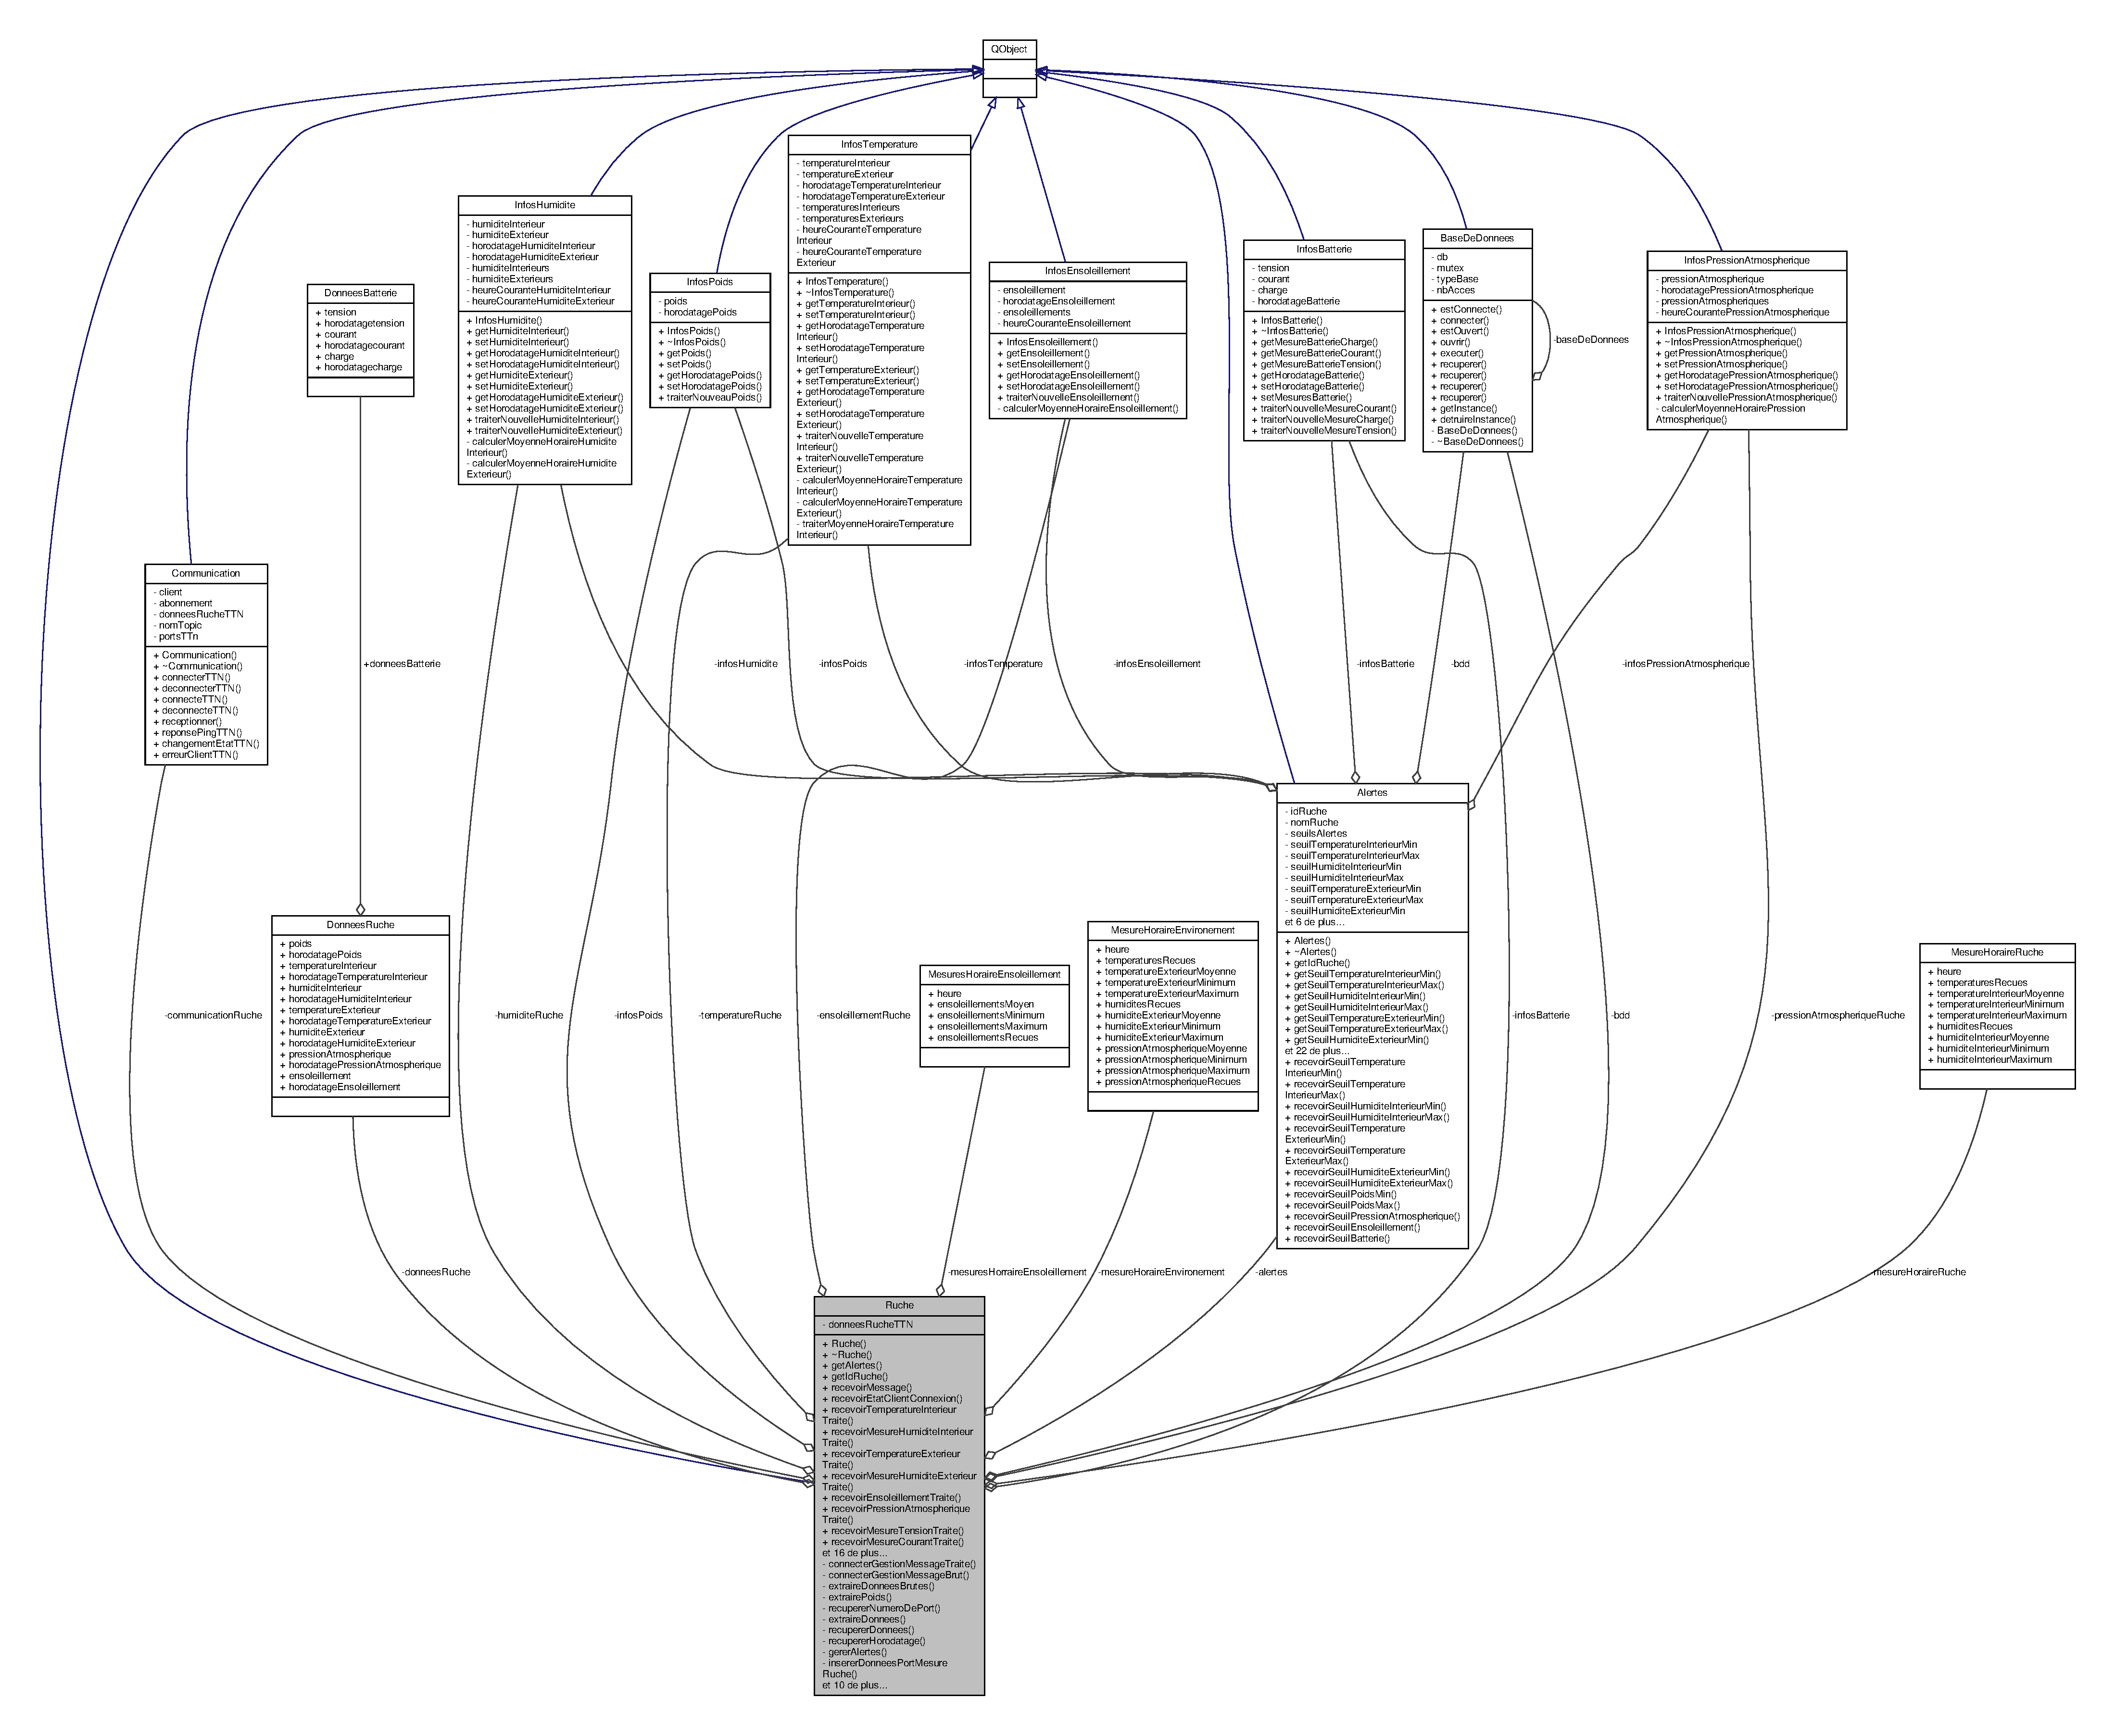
\includegraphics[width=350pt]{class_ruche__coll__graph}
\end{center}
\end{figure}
\subsubsection*{Connecteurs publics}
\begin{DoxyCompactItemize}
\item 
void \hyperlink{class_ruche_a05a34e78d360609f772b9a37c69d0043}{recevoir\+Message} (const Q\+Byte\+Array \&message, const Q\+Mqtt\+Topic\+Name \&topic)
\begin{DoxyCompactList}\small\item\em slot recevant les données \end{DoxyCompactList}\item 
void \hyperlink{class_ruche_a1224416341dc2b33418dd296327ae410}{recevoir\+Etat\+Client\+Connexion} (bool)
\item 
void \hyperlink{class_ruche_a3a5934e6da843c959f34aecef1217f92}{recevoir\+Temperature\+Interieur\+Traite} (double temperature\+Interieur, Q\+String horodatage)
\begin{DoxyCompactList}\small\item\em slot recevant la temperature interieur traite \end{DoxyCompactList}\item 
void \hyperlink{class_ruche_aab8b4958b32aad9af790963903e4788e}{recevoir\+Mesure\+Humidite\+Interieur\+Traite} (double humidite\+Interieur\+Traite, Q\+String horodatage)
\item 
void \hyperlink{class_ruche_a1d9b1d3aad20f206f27de4093b4a136f}{recevoir\+Temperature\+Exterieur\+Traite} (double temperature\+Exterieur, Q\+String horodatage)
\begin{DoxyCompactList}\small\item\em slot recevant la temperature exterieur traite \end{DoxyCompactList}\item 
void \hyperlink{class_ruche_a2d19d8438eae55c1d76691398087f079}{recevoir\+Mesure\+Humidite\+Exterieur\+Traite} (double humidite\+Exterieur\+Traite, Q\+String horodatage)
\item 
void \hyperlink{class_ruche_a581320fbd44c1752d10aa0e6e533863c}{recevoir\+Ensoleillement\+Traite} (double ensoleillement, Q\+String horodatage)
\begin{DoxyCompactList}\small\item\em slot recevant l\textquotesingle{}ensoleillement traite \end{DoxyCompactList}\item 
void \hyperlink{class_ruche_a3b43ce547e616ee0b14e3a0e0aa44a4d}{recevoir\+Pression\+Atmospherique\+Traite} (double pression\+Atmospherique, Q\+String horodatage)
\item 
void \hyperlink{class_ruche_a65782ea2ee63003f2eae45e2530e3d5b}{recevoir\+Mesure\+Tension\+Traite} (double tension, Q\+String)
\item 
void \hyperlink{class_ruche_a9e416457e8712d353580b7b242ef0836}{recevoir\+Mesure\+Courant\+Traite} (double courant, Q\+String)
\item 
void \hyperlink{class_ruche_a4ad540139115b79cd52336ad1a11453c}{recevoir\+Mesure\+Charge\+Traite} (double charge, Q\+String)
\item 
void \hyperlink{class_ruche_afd8b0d7512f325327704cd3e37091dc2}{recevoir\+Mesure\+Poids\+Traite} (double poids, Q\+String)
\item 
void \hyperlink{class_ruche_a2d2a681916140b977d45423d0d5d7b34}{recevoir\+Traitement\+Temperature\+Interieur} (const double temperature\+Interieur\+Moyenne, const double temperature\+Interieur\+Minimum, const double temperature\+Interieur\+Maximum, int heure)
\item 
void \hyperlink{class_ruche_a8482dda95a8a7888d5a60ea6f7d8729e}{recevoir\+Traitement\+Temperature\+Exterieur} (const double temperature\+Exterieur\+Moyenne, const double temperature\+Exterieur\+Minimum, const double temperature\+Exterieur\+Maximum, int heure)
\item 
void \hyperlink{class_ruche_a6d4c59f2850f803a0ed1946e737b4262}{recevoir\+Traitement\+Humidite\+Interieur} (const double temperature\+Interieur\+Moyenne, const double temperature\+Interieur\+Minimum, const double temperature\+Interieur\+Maximum, int heure)
\item 
void \hyperlink{class_ruche_a59e89246b484d7b63851c0ebd20af6c5}{recevoir\+Traitement\+Humidite\+Exterieur} (const double humidite\+Exterieurs\+Moyenne, const double humidite\+Exterieurs\+Minimum, const double humidite\+Exterieurs\+Maximum, int heure)
\item 
void \hyperlink{class_ruche_aa42daeffa023c83fde40072601e1fa39}{recevoir\+Traitement\+Pression\+Atmospherique} (const double pression\+Atmospherique\+Moyenne, const double pression\+Atmospherique\+Minimum, const double pression\+Atmospherique\+Maximum, int heure)
\item 
void \hyperlink{class_ruche_a2ac5766ce8652084f034c498691488ea}{recevoir\+Traitement\+Ensoleillement} (const double ensoleillements\+Moyen, const double ensoleillements\+Minimum, const double temperature\+Exterieur\+Maximum, int heure)
\item 
void \hyperlink{class_ruche_a2984c1e492d1ceacd3081e39a4f8cc26}{recevoir\+Alertes\+Temperature\+Interieur} (\hyperlink{parametres_8h_aaa6de8207c94675264c90b10b613368d}{Seuils\+Alertes} seuils\+Alertes)
\item 
void \hyperlink{class_ruche_af09b04e9a415ad3df9941068b74046fc}{recevoir\+Alertes\+Temperature\+Exterieur} (\hyperlink{parametres_8h_aaa6de8207c94675264c90b10b613368d}{Seuils\+Alertes} seuils\+Alertes)
\item 
void \hyperlink{class_ruche_af7b500ef1469f689dfe6b78ae6e3c025}{recevoir\+Alertes\+Humidite\+Interieur} (\hyperlink{parametres_8h_aaa6de8207c94675264c90b10b613368d}{Seuils\+Alertes} seuils\+Alertes)
\item 
void \hyperlink{class_ruche_a6b12ebe7e83f12b31e49b44e25fdfa58}{recevoir\+Alertes\+Humidite\+Exterieur} (\hyperlink{parametres_8h_aaa6de8207c94675264c90b10b613368d}{Seuils\+Alertes} seuils\+Alertes)
\item 
void \hyperlink{class_ruche_aa649f21e5d2a196bc7fbc570dc731ade}{recevoir\+Alertes\+Pression\+Atmospherique} (\hyperlink{parametres_8h_aaa6de8207c94675264c90b10b613368d}{Seuils\+Alertes} seuils\+Alertes)
\item 
void \hyperlink{class_ruche_aa5dc6e5c65d0a685dcaa1c698b25e938}{recevoir\+Alertes\+Poids} (\hyperlink{parametres_8h_aaa6de8207c94675264c90b10b613368d}{Seuils\+Alertes})
\item 
void \hyperlink{class_ruche_afdfb0cff676b6de5f421aed01c3d49db}{recevoir\+Alertes\+Ensoleillement} (\hyperlink{parametres_8h_aaa6de8207c94675264c90b10b613368d}{Seuils\+Alertes}, double niveau\+Ensoleillement)
\item 
void \hyperlink{class_ruche_aee278a316c2e462e43705e15a36ab43f}{recevoir\+Alertes\+Batterie} (\hyperlink{parametres_8h_aaa6de8207c94675264c90b10b613368d}{Seuils\+Alertes}, double)
\end{DoxyCompactItemize}
\subsubsection*{Signaux}
\begin{DoxyCompactItemize}
\item 
void \hyperlink{class_ruche_abe5e5d4f4070766d5295d4dc6e0ce03c}{nouvelle\+Mesure\+Poids} (Q\+String poids, Q\+String horodatage\+Poids)
\begin{DoxyCompactList}\small\item\em signal vers la classe \hyperlink{class_infos_poids}{Infos\+Poids} \end{DoxyCompactList}\item 
void \hyperlink{class_ruche_ac4d6e0c0db4b5c992606bff88759b2c3}{nouvelle\+Temperature\+Interieur} (Q\+String temperature\+Interieur, Q\+String horodatage)
\begin{DoxyCompactList}\small\item\em signal vers la classe \hyperlink{class_infos_temperature}{Infos\+Temperature} \end{DoxyCompactList}\item 
void \hyperlink{class_ruche_a1d5094246e935d8ae5b9f08c9d042247}{nouvelle\+Humidite\+Interieur} (Q\+String humidite\+Interieur, Q\+String horodatage)
\begin{DoxyCompactList}\small\item\em signal vers la classe \hyperlink{class_infos_humidite}{Infos\+Humidite} \end{DoxyCompactList}\item 
void \hyperlink{class_ruche_aa8d28f554cd485c32d348a9147d2e236}{nouvelle\+Temperature\+Exterieur} (Q\+String temperature\+Exterieur, Q\+String horodatage)
\begin{DoxyCompactList}\small\item\em signal vers la classe \hyperlink{class_infos_temperature}{Infos\+Temperature} \end{DoxyCompactList}\item 
void \hyperlink{class_ruche_af88c6ed0320bfe45d5b15faa936caf4d}{nouvelle\+Humidite\+Exterieur} (Q\+String humidite\+Exterieur, Q\+String horodatage)
\begin{DoxyCompactList}\small\item\em signal vers la classe \hyperlink{class_infos_humidite}{Infos\+Humidite} \end{DoxyCompactList}\item 
void \hyperlink{class_ruche_ae72c86953df530bc5d3901ba66cf884d}{nouvelle\+Pression\+Atmospherique} (Q\+String pression\+Atmospherique, Q\+String horodatage)
\begin{DoxyCompactList}\small\item\em signal vers la classe \hyperlink{class_infos_pression_atmospherique}{Infos\+Pression\+Atmospherique} \end{DoxyCompactList}\item 
void \hyperlink{class_ruche_aa9eaf4dd1b60e525c7d1bb5319130ce1}{nouvelle\+Mesure\+Ensoleillement} (Q\+String ensoleillement, Q\+String horodatage)
\begin{DoxyCompactList}\small\item\em signal vers la classe \hyperlink{class_infos_ensoleillement}{Infos\+Ensoleillement} \end{DoxyCompactList}\item 
void \hyperlink{class_ruche_a49ac0c627ecac39c969403db1495711f}{nouvelle\+Mesure\+Charge} (Q\+String charge, Q\+String horodatage)
\item 
void \hyperlink{class_ruche_a46d8191444302b02a52d1128c5650730}{nouvelle\+Mesure\+Courant} (Q\+String courant, Q\+String horodatage)
\item 
void \hyperlink{class_ruche_aa3fd352b343fcf780787aeb7e42935ef}{nouvelle\+Mesure\+Tension} (Q\+String tension, Q\+String horodatage)
\item 
void \hyperlink{class_ruche_aa63b4fd7c695ef77c9ff4b684ed8ce91}{nouvelle\+Mesure\+Temperature\+Interieur\+Traite} (double temperature\+Interieur\+Traite, Q\+String horodatage)
\begin{DoxyCompactList}\small\item\em signal vers la classe \hyperlink{class_ruche_ihm}{Ruche\+Ihm} \end{DoxyCompactList}\item 
void \hyperlink{class_ruche_abb16e6c9eef6640a3a216f856cf8d0f5}{nouvelle\+Mesure\+Humidite\+Interieur\+Traite} (double humidite\+Interieur\+Traite, Q\+String horodatage)
\begin{DoxyCompactList}\small\item\em signal vers la classe \hyperlink{class_ruche_ihm}{Ruche\+Ihm} \end{DoxyCompactList}\item 
void \hyperlink{class_ruche_a5b85ea246b58776a96e2ff7bd701daa7}{nouvelle\+Mesure\+Temperature\+Exterieur\+Traite} (double temperature\+Exterieur, Q\+String horodatage)
\begin{DoxyCompactList}\small\item\em signal vers la classe \hyperlink{class_ruche_ihm}{Ruche\+Ihm} \end{DoxyCompactList}\item 
void \hyperlink{class_ruche_a9dc15aec6973ca8f565960a51f7f0a6b}{nouvelle\+Mesure\+Humidite\+Exterieur\+Traite} (double humidite\+Exterieur\+Traite, Q\+String horodatage)
\begin{DoxyCompactList}\small\item\em signal vers la classe \hyperlink{class_ruche_ihm}{Ruche\+Ihm} \end{DoxyCompactList}\item 
void \hyperlink{class_ruche_ac0cf9ceae0a82739dbb4c2d33c4a2494}{nouvelle\+Mesure\+Ensoleillement\+Traite} (double ensoleillement, Q\+String horodatage)
\begin{DoxyCompactList}\small\item\em signal vers la classe \hyperlink{class_ruche_ihm}{Ruche\+Ihm} \end{DoxyCompactList}\item 
void \hyperlink{class_ruche_ac55a1301b55166474b700ee0a2a57f22}{nouvelle\+Pression\+Atmospherique\+Traite} (double pression\+Atmospherique, Q\+String horodatage)
\begin{DoxyCompactList}\small\item\em signal vers la classe \hyperlink{class_ruche_ihm}{Ruche\+Ihm} \end{DoxyCompactList}\item 
void \hyperlink{class_ruche_abe4e46c9a1b6e8cfb6adb2e958d9ab83}{nouvelle\+Mesure\+Tension} (double tension, Q\+String horodatage)
\item 
void \hyperlink{class_ruche_a189654383ee5802ccdc4256f2c1171c7}{nouvelle\+Mesure\+Courant} (double courant, Q\+String horodatage)
\item 
void \hyperlink{class_ruche_a3bd0a55bb10880f8753d5c2fdb41651f}{nouvelle\+Mesure\+Charge} (double charge, Q\+String horodatage)
\item 
void \hyperlink{class_ruche_a094d288ac798e0011e29242db0c7a34e}{nouvelle\+Mesure\+Poids} (double poids, Q\+String horodatage)
\item 
void \hyperlink{class_ruche_a5fdf12cb02acc7283f183a7aad906edc}{nouvelle\+Mesure\+Temperature\+Interieur\+Traite\+Par\+Heure} ()
\item 
void \hyperlink{class_ruche_ac0d7e104549abdfa87691618aba6291b}{nouvelle\+Mesure\+Temperature\+Exterieur\+Traite\+Par\+Heure} ()
\item 
void \hyperlink{class_ruche_a02a3e68fd11b208507867ebd0e8dbdc2}{nouvelle\+Mesure\+Humidite\+Interieur\+Traite\+Par\+Heure} ()
\item 
void \hyperlink{class_ruche_aab1ad40a46ab5fe4352a23e4a986856b}{nouvelle\+Mesure\+Humidite\+Exterieur\+Traite\+Par\+Heure} ()
\item 
void \hyperlink{class_ruche_a7948d81996c196eeb0f20dc203a52e75}{nouvelle\+Mesure\+Pression\+Atmospherique\+Traite\+Par\+Heure} ()
\item 
void \hyperlink{class_ruche_adab3ce6ee33b3e6306aa7dc4f2ca1f20}{nouvelle\+Mesure\+Ensoleillement\+Traite\+Par\+Heure} ()
\item 
void \hyperlink{class_ruche_ac2f37831cb8c70ac4df2a3ac805b728b}{envoi\+Alertes\+Temperature\+Interieur} (\hyperlink{parametres_8h_aaa6de8207c94675264c90b10b613368d}{Seuils\+Alertes})
\item 
void \hyperlink{class_ruche_a5bb36a4bb9692a744a1b7ebc5fc59f57}{envoi\+Alertes\+Temperature\+Exterieur} (\hyperlink{parametres_8h_aaa6de8207c94675264c90b10b613368d}{Seuils\+Alertes})
\item 
void \hyperlink{class_ruche_a0f1dfe6d0a677341e29296e044d91975}{envoi\+Alertes\+Humidite\+Interieur} (\hyperlink{parametres_8h_aaa6de8207c94675264c90b10b613368d}{Seuils\+Alertes})
\item 
void \hyperlink{class_ruche_abef2fd2fdeaee8bc19fa1ce13b32f4d0}{envoi\+Alertes\+Humidite\+Exterieur} (\hyperlink{parametres_8h_aaa6de8207c94675264c90b10b613368d}{Seuils\+Alertes})
\item 
void \hyperlink{class_ruche_a97ae09a121944f7df48fb38bd049b878}{envoi\+Alertes\+Pression\+Atmospherique} (\hyperlink{parametres_8h_aaa6de8207c94675264c90b10b613368d}{Seuils\+Alertes})
\item 
void \hyperlink{class_ruche_a21d7f05b696896b1a3c7e20c396aaf23}{envoi\+Alertes\+Poids} (\hyperlink{parametres_8h_aaa6de8207c94675264c90b10b613368d}{Seuils\+Alertes})
\item 
void \hyperlink{class_ruche_aa3d500a4a0e5ed60da000af15000505e}{envoi\+Alertes\+Ensoleillement} (\hyperlink{parametres_8h_aaa6de8207c94675264c90b10b613368d}{Seuils\+Alertes}, double)
\item 
void \hyperlink{class_ruche_ac76ce5692e134b365330d91af2a6b4e7}{envoi\+Alertes\+Batterie} (\hyperlink{parametres_8h_aaa6de8207c94675264c90b10b613368d}{Seuils\+Alertes}, double)
\item 
void \hyperlink{class_ruche_a932b2c69dbe919afed9549d5666b2736}{etat\+Client\+Connexion} (bool connexion)
\item 
void \hyperlink{class_ruche_a2a0f122bfd939419f40facf41e91fe30}{envoi\+Localisation\+Passerelle} (Q\+String longitude, Q\+String latitude)
\end{DoxyCompactItemize}
\subsubsection*{Fonctions membres publiques}
\begin{DoxyCompactItemize}
\item 
\hyperlink{class_ruche_a8b4ee3752d984c5acee93b990db7939a}{Ruche} (Q\+String\+List \hyperlink{class_ruche_a4556832042641c08a6ef2ab9d80d771e}{donnees\+Ruche\+T\+TN}, \hyperlink{class_q_object}{Q\+Object} $\ast$parent=0)
\item 
\hyperlink{class_ruche_ad3f950d0731f9801f06dd6ae09f2e5fa}{$\sim$\+Ruche} ()
\begin{DoxyCompactList}\small\item\em Destructeur de la classe \hyperlink{class_ruche}{Ruche}. \end{DoxyCompactList}\item 
\hyperlink{class_alertes}{Alertes} $\ast$ \hyperlink{class_ruche_a9edbc2e81ccb2cb76de43639bcb16ec1}{get\+Alertes} ()
\item 
Q\+String \hyperlink{class_ruche_a9f2de5ef29557ec7a53d5e22df34d164}{get\+Id\+Ruche} ()
\end{DoxyCompactItemize}
\subsubsection*{Fonctions membres privées}
\begin{DoxyCompactItemize}
\item 
void \hyperlink{class_ruche_a20ec8c6dc931218e5cf682050fe845d9}{connecter\+Gestion\+Message\+Traite} ()
\item 
void \hyperlink{class_ruche_a9c8e7e3b529676c6dda3d936370af00f}{connecter\+Gestion\+Message\+Brut} ()
\begin{DoxyCompactList}\small\item\em methode regroupant les conection des messages brut \end{DoxyCompactList}\item 
Q\+String \hyperlink{class_ruche_a97d167a57144e9d923007b732d4e6091}{extraire\+Donnees\+Brutes} (const Q\+Byte\+Array \&message)
\item 
Q\+String \hyperlink{class_ruche_a309bff2fac1f8562da0f5f1a5d75c907}{extraire\+Poids} (const Q\+String \&donnees\+Brutes)
\item 
\hyperlink{parametres_8h_a0fe68caa1e9147addc96657cc822b937}{Ports\+T\+TN} \hyperlink{class_ruche_a157782119650e2bd196612c3fa66972c}{recuperer\+Numero\+De\+Port} (Q\+Byte\+Array message)
\begin{DoxyCompactList}\small\item\em recuperer le numero de port \end{DoxyCompactList}\item 
void \hyperlink{class_ruche_a21c0dafeaec03d451590037343e6a3ca}{extraire\+Donnees} (\hyperlink{parametres_8h_a0fe68caa1e9147addc96657cc822b937}{Ports\+T\+TN} port, Q\+Byte\+Array message)
\begin{DoxyCompactList}\small\item\em extait les données \end{DoxyCompactList}\item 
Q\+String \hyperlink{class_ruche_a68e487fc714c68b7d4f761cad9122b39}{recuperer\+Donnees} (Q\+Byte\+Array message, Q\+String objet\+Json, Q\+String sous\+Objet\+Json)
\begin{DoxyCompactList}\small\item\em recuperer les données \end{DoxyCompactList}\item 
Q\+String \hyperlink{class_ruche_a072193021274bb4308776934c35f7443}{recuperer\+Horodatage} (Q\+Byte\+Array message, Q\+String objet\+Json, Q\+String sous\+Objet\+Json)
\begin{DoxyCompactList}\small\item\em recuperer l\textquotesingle{}horodatage \end{DoxyCompactList}\item 
void \hyperlink{class_ruche_a80f3538f081aea887d7199f114dfca01}{gerer\+Alertes} ()
\item 
void \hyperlink{class_ruche_aa61f6dd8b15e5242ef3a3bdd87cca4a3}{inserer\+Donnees\+Port\+Mesure\+Ruche} ()
\item 
void \hyperlink{class_ruche_a46c0f440f40a5125f2d579b481660457}{inserer\+Donnees\+Port\+Mesure\+Environnement} ()
\item 
void \hyperlink{class_ruche_ad21de5f7d48195be0658f52c55f34183}{inserer\+Donnees\+Port\+Ensoleillement} ()
\item 
void \hyperlink{class_ruche_a923f42fc4878a01f6102966a748e8f37}{inserer\+Donnees\+Port\+Poids} ()
\item 
void \hyperlink{class_ruche_a509367d6b2bcb7e6431fc1cc5ff606b5}{inserer\+Donnees\+Port\+Batterie} ()
\item 
void \hyperlink{class_ruche_a3a093c088d9c97f347394c8a681f7302}{inserer\+Mesure\+Horaire\+Ruche} ()
\item 
void \hyperlink{class_ruche_ac52e79446c5629645e02e27d2a01e56c}{inserer\+Mesure\+Horaire\+Environnement} ()
\item 
void \hyperlink{class_ruche_a658234b9d96541d204b95b74556742b6}{inserer\+Mesure\+Horaire\+Ensoleillement} ()
\item 
void \hyperlink{class_ruche_a01759e2b2d37ddf0a91b50182c5f26f2}{inserer\+Mesure\+Horaire\+Poids} ()
\item 
void \hyperlink{class_ruche_a4af7e7c209b2267daf1f640cb53020e2}{inserer\+Mesure\+Horaire\+Batterie} ()
\item 
void \hyperlink{class_ruche_abdb0503e660631a0a9d2ed7177918341}{recuperer\+Localisation\+Passerelle} (Q\+Byte\+Array message)
\end{DoxyCompactItemize}
\subsubsection*{Attributs privés}
\begin{DoxyCompactItemize}
\item 
\hyperlink{class_infos_ensoleillement}{Infos\+Ensoleillement} $\ast$ \hyperlink{class_ruche_a197003ecff4f029885c7d38569a68d49}{ensoleillement\+Ruche}
\item 
\hyperlink{class_infos_humidite}{Infos\+Humidite} $\ast$ \hyperlink{class_ruche_acb380928928e693a1933c4cf607ddf80}{humidite\+Ruche}
\item 
\hyperlink{class_infos_pression_atmospherique}{Infos\+Pression\+Atmospherique} $\ast$ \hyperlink{class_ruche_a06efa82900dc7e31ed67c826d3157ae0}{pression\+Atmospherique\+Ruche}
\item 
\hyperlink{class_infos_temperature}{Infos\+Temperature} $\ast$ \hyperlink{class_ruche_af721fb92f801a9b1f3ef3aa9867cf3de}{temperature\+Ruche}
\item 
\hyperlink{class_infos_batterie}{Infos\+Batterie} $\ast$ \hyperlink{class_ruche_af34340e456aff54c8d1ec433fdbe0740}{infos\+Batterie}
\item 
\hyperlink{class_infos_poids}{Infos\+Poids} $\ast$ \hyperlink{class_ruche_af3d02b62dd3d986b73b38851bb88ec77}{infos\+Poids}
\item 
\hyperlink{class_communication}{Communication} $\ast$ \hyperlink{class_ruche_a6211b7b8f43abf5eecf8a1fc2d0f037e}{communication\+Ruche}
\item 
\hyperlink{class_base_de_donnees}{Base\+De\+Donnees} $\ast$ \hyperlink{class_ruche_a8577fdedabdecd98652e338e83bb3b65}{bdd}
\begin{DoxyCompactList}\small\item\em agrégation de l\textquotesingle{}objet \hyperlink{class_base_de_donnees}{Base\+De\+Donnees} \end{DoxyCompactList}\item 
\hyperlink{class_alertes}{Alertes} $\ast$ \hyperlink{class_ruche_af07644ddce44cb5ed4286475dc0f9d46}{alertes}
\item 
Q\+String\+List \hyperlink{class_ruche_a4556832042641c08a6ef2ab9d80d771e}{donnees\+Ruche\+T\+TN}
\item 
\hyperlink{struct_donnees_ruche}{Donnees\+Ruche} \hyperlink{class_ruche_a1526bfa78f03e0710ad16f880a40c15f}{donnees\+Ruche}
\item 
\hyperlink{struct_mesure_horaire_ruche}{Mesure\+Horaire\+Ruche} \hyperlink{class_ruche_a9a68d3b7eb272e139f1532fdcbca2da3}{mesure\+Horaire\+Ruche}
\item 
\hyperlink{struct_mesure_horaire_environement}{Mesure\+Horaire\+Environement} \hyperlink{class_ruche_a73a826506110c10d9221065670985e52}{mesure\+Horaire\+Environement}
\item 
\hyperlink{struct_mesures_horaire_ensoleillement}{Mesures\+Horaire\+Ensoleillement} \hyperlink{class_ruche_a5e57df1ce7805b1ab0f6d8ef37504582}{mesures\+Horraire\+Ensoleillement}
\end{DoxyCompactItemize}


\subsubsection{Description détaillée}
\begin{DoxyAuthor}{Auteur}
Florentin Mellah, Enzo Rossi
\end{DoxyAuthor}
\begin{DoxyVersion}{Version}
1.\+1 
\end{DoxyVersion}


\subsubsection{Documentation des constructeurs et destructeur}
\mbox{\Hypertarget{class_ruche_a8b4ee3752d984c5acee93b990db7939a}\label{class_ruche_a8b4ee3752d984c5acee93b990db7939a}} 
\index{Ruche@{Ruche}!Ruche@{Ruche}}
\index{Ruche@{Ruche}!Ruche@{Ruche}}
\paragraph{\texorpdfstring{Ruche()}{Ruche()}}
{\footnotesize\ttfamily Ruche\+::\+Ruche (\begin{DoxyParamCaption}\item[{Q\+String\+List}]{donnees\+Ruche\+T\+TN,  }\item[{\hyperlink{class_q_object}{Q\+Object} $\ast$}]{parent = {\ttfamily 0} }\end{DoxyParamCaption})}



Références \hyperlink{class_ruche_af07644ddce44cb5ed4286475dc0f9d46}{alertes}, \hyperlink{class_ruche_a8577fdedabdecd98652e338e83bb3b65}{bdd}, \hyperlink{parametres_8h_a45f8f15b8f9a7ab4c2b219038ff64f6b}{B\+D\+D\+\_\+\+N\+O\+M\+B\+A\+SE}, \hyperlink{parametres_8h_ae2ded9166ed2553182545e97514c04f7}{B\+D\+D\+\_\+\+P\+A\+S\+S\+W\+O\+RD}, \hyperlink{parametres_8h_a423559dc987673b8aacaa9f369839bb0}{B\+D\+D\+\_\+\+S\+E\+R\+V\+E\+UR}, \hyperlink{parametres_8h_a88b5f5b81fa534553c68802384beff2c}{B\+D\+D\+\_\+\+U\+S\+E\+R\+N\+A\+ME}, \hyperlink{class_ruche_a6211b7b8f43abf5eecf8a1fc2d0f037e}{communication\+Ruche}, \hyperlink{class_base_de_donnees_ac20da193923a9bfea5e38ee5a54820cd}{Base\+De\+Donnees\+::connecter()}, \hyperlink{class_ruche_a9c8e7e3b529676c6dda3d936370af00f}{connecter\+Gestion\+Message\+Brut()}, \hyperlink{class_ruche_a20ec8c6dc931218e5cf682050fe845d9}{connecter\+Gestion\+Message\+Traite()}, \hyperlink{class_ruche_a4556832042641c08a6ef2ab9d80d771e}{donnees\+Ruche\+T\+TN}, \hyperlink{class_ruche_a197003ecff4f029885c7d38569a68d49}{ensoleillement\+Ruche}, \hyperlink{class_base_de_donnees_a00388973f3ec42e5c8e76e7af7e124b2}{Base\+De\+Donnees\+::est\+Connecte()}, \hyperlink{class_ruche_a932b2c69dbe919afed9549d5666b2736}{etat\+Client\+Connexion()}, \hyperlink{class_ruche_a80f3538f081aea887d7199f114dfca01}{gerer\+Alertes()}, \hyperlink{class_base_de_donnees_a80028aa2b6b4fbf30fb2e36357b7d3d3}{Base\+De\+Donnees\+::get\+Instance()}, \hyperlink{class_ruche_acb380928928e693a1933c4cf607ddf80}{humidite\+Ruche}, \hyperlink{class_ruche_af34340e456aff54c8d1ec433fdbe0740}{infos\+Batterie}, \hyperlink{class_ruche_af3d02b62dd3d986b73b38851bb88ec77}{infos\+Poids}, \hyperlink{class_ruche_a06efa82900dc7e31ed67c826d3157ae0}{pression\+Atmospherique\+Ruche}, \hyperlink{class_ruche_a1224416341dc2b33418dd296327ae410}{recevoir\+Etat\+Client\+Connexion()}, \hyperlink{class_ruche_a05a34e78d360609f772b9a37c69d0043}{recevoir\+Message()}, \hyperlink{class_alertes_a8bbe30ddc4893f943781749917b23463}{Alertes\+::set\+Infos\+Batterie()}, \hyperlink{class_alertes_a5379fc65522a77dc2cc110e489e1469d}{Alertes\+::set\+Infos\+Ensoleillement()}, \hyperlink{class_alertes_a05734ac9e97a9001de4ce9ef96235c87}{Alertes\+::set\+Infos\+Humidite()}, \hyperlink{class_alertes_a100bad47769994abc976419a355c4a26}{Alertes\+::set\+Infos\+Poids()}, \hyperlink{class_alertes_a771133f26d4ab8c90d1bdf50e1d23d87}{Alertes\+::set\+Infos\+Pression\+Atmospherique()}, \hyperlink{class_alertes_a091a0fabca5b06302bc19de31aecafff}{Alertes\+::set\+Infos\+Temperature()}, et \hyperlink{class_ruche_af721fb92f801a9b1f3ef3aa9867cf3de}{temperature\+Ruche}.


\begin{DoxyCode}
00043                                                          : \hyperlink{class_q_object}{QObject}(parent), 
      \hyperlink{class_ruche_a197003ecff4f029885c7d38569a68d49}{ensoleillementRuche}(0), \hyperlink{class_ruche_acb380928928e693a1933c4cf607ddf80}{humiditeRuche}(0), 
      \hyperlink{class_ruche_a06efa82900dc7e31ed67c826d3157ae0}{pressionAtmospheriqueRuche}(0), \hyperlink{class_ruche_af721fb92f801a9b1f3ef3aa9867cf3de}{temperatureRuche}(0), 
      \hyperlink{class_ruche_af34340e456aff54c8d1ec433fdbe0740}{infosBatterie}(0), \hyperlink{class_ruche_af3d02b62dd3d986b73b38851bb88ec77}{infosPoids}(0), \hyperlink{class_ruche_a6211b7b8f43abf5eecf8a1fc2d0f037e}{communicationRuche}(0), 
      \hyperlink{class_ruche_af07644ddce44cb5ed4286475dc0f9d46}{alertes}(0), \hyperlink{class_ruche_a4556832042641c08a6ef2ab9d80d771e}{donneesRucheTTN}(\hyperlink{class_ruche_a4556832042641c08a6ef2ab9d80d771e}{donneesRucheTTN})
00044 \{
00045     qDebug()<< Q\_FUNC\_INFO << \textcolor{stringliteral}{"donneesRucheTTN"} << \hyperlink{class_ruche_a4556832042641c08a6ef2ab9d80d771e}{donneesRucheTTN};
00046     \hyperlink{class_ruche_a8577fdedabdecd98652e338e83bb3b65}{bdd} = \hyperlink{class_base_de_donnees_a80028aa2b6b4fbf30fb2e36357b7d3d3}{BaseDeDonnees::getInstance}();
00047     \textcolor{keywordflow}{if}(!\hyperlink{class_ruche_a8577fdedabdecd98652e338e83bb3b65}{bdd}->\hyperlink{class_base_de_donnees_a00388973f3ec42e5c8e76e7af7e124b2}{estConnecte}())
00048         \hyperlink{class_ruche_a8577fdedabdecd98652e338e83bb3b65}{bdd}->\hyperlink{class_base_de_donnees_ac20da193923a9bfea5e38ee5a54820cd}{connecter}(\hyperlink{parametres_8h_a45f8f15b8f9a7ab4c2b219038ff64f6b}{BDD\_NOMBASE}, \hyperlink{parametres_8h_a88b5f5b81fa534553c68802384beff2c}{BDD\_USERNAME}, 
      \hyperlink{parametres_8h_ae2ded9166ed2553182545e97514c04f7}{BDD\_PASSWORD}, \hyperlink{parametres_8h_a423559dc987673b8aacaa9f369839bb0}{BDD\_SERVEUR});
00049 
00050     \hyperlink{class_ruche_af34340e456aff54c8d1ec433fdbe0740}{infosBatterie} = \textcolor{keyword}{new} \hyperlink{class_infos_batterie}{InfosBatterie}(\textcolor{keyword}{this});
00051     \hyperlink{class_ruche_af3d02b62dd3d986b73b38851bb88ec77}{infosPoids} = \textcolor{keyword}{new} \hyperlink{class_infos_poids}{InfosPoids}(\textcolor{keyword}{this});
00052     \hyperlink{class_ruche_a197003ecff4f029885c7d38569a68d49}{ensoleillementRuche} = \textcolor{keyword}{new} \hyperlink{class_infos_ensoleillement}{InfosEnsoleillement}(\textcolor{keyword}{this});
00053     \hyperlink{class_ruche_acb380928928e693a1933c4cf607ddf80}{humiditeRuche} = \textcolor{keyword}{new} \hyperlink{class_infos_humidite}{InfosHumidite}(\textcolor{keyword}{this});
00054     \hyperlink{class_ruche_a06efa82900dc7e31ed67c826d3157ae0}{pressionAtmospheriqueRuche} = \textcolor{keyword}{new} 
      \hyperlink{class_infos_pression_atmospherique}{InfosPressionAtmospherique}(\textcolor{keyword}{this});
00055     \hyperlink{class_ruche_af721fb92f801a9b1f3ef3aa9867cf3de}{temperatureRuche} = \textcolor{keyword}{new} \hyperlink{class_infos_temperature}{InfosTemperature}(\textcolor{keyword}{this});
00056 
00057     \hyperlink{class_ruche_a6211b7b8f43abf5eecf8a1fc2d0f037e}{communicationRuche} = \textcolor{keyword}{new} \hyperlink{class_communication}{Communication}(donneesRucheTTN);
00058 
00059     \hyperlink{class_ruche_af07644ddce44cb5ed4286475dc0f9d46}{alertes} = \textcolor{keyword}{new} \hyperlink{class_alertes}{Alertes}(donneesRucheTTN.at(0), donneesRucheTTN.at(1), \textcolor{keyword}{this});
00060 
00061     \hyperlink{class_ruche_af07644ddce44cb5ed4286475dc0f9d46}{alertes}->\hyperlink{class_alertes_a8bbe30ddc4893f943781749917b23463}{setInfosBatterie}(\hyperlink{class_ruche_af34340e456aff54c8d1ec433fdbe0740}{infosBatterie});
00062     \hyperlink{class_ruche_af07644ddce44cb5ed4286475dc0f9d46}{alertes}->\hyperlink{class_alertes_a100bad47769994abc976419a355c4a26}{setInfosPoids}(\hyperlink{class_ruche_af3d02b62dd3d986b73b38851bb88ec77}{infosPoids});
00063     \hyperlink{class_ruche_af07644ddce44cb5ed4286475dc0f9d46}{alertes}->\hyperlink{class_alertes_a5379fc65522a77dc2cc110e489e1469d}{setInfosEnsoleillement}(
      \hyperlink{class_ruche_a197003ecff4f029885c7d38569a68d49}{ensoleillementRuche});
00064     \hyperlink{class_ruche_af07644ddce44cb5ed4286475dc0f9d46}{alertes}->\hyperlink{class_alertes_a05734ac9e97a9001de4ce9ef96235c87}{setInfosHumidite}(\hyperlink{class_ruche_acb380928928e693a1933c4cf607ddf80}{humiditeRuche});
00065     \hyperlink{class_ruche_af07644ddce44cb5ed4286475dc0f9d46}{alertes}->\hyperlink{class_alertes_a771133f26d4ab8c90d1bdf50e1d23d87}{setInfosPressionAtmospherique}(
      \hyperlink{class_ruche_a06efa82900dc7e31ed67c826d3157ae0}{pressionAtmospheriqueRuche});
00066     \hyperlink{class_ruche_af07644ddce44cb5ed4286475dc0f9d46}{alertes}->\hyperlink{class_alertes_a091a0fabca5b06302bc19de31aecafff}{setInfosTemperature}(\hyperlink{class_ruche_af721fb92f801a9b1f3ef3aa9867cf3de}{temperatureRuche});
00067 
00068     \hyperlink{class_ruche_a9c8e7e3b529676c6dda3d936370af00f}{connecterGestionMessageBrut}();
00069     \hyperlink{class_ruche_a20ec8c6dc931218e5cf682050fe845d9}{connecterGestionMessageTraite}();
00070     \hyperlink{class_ruche_a80f3538f081aea887d7199f114dfca01}{gererAlertes}();
00071 
00072     connect(\hyperlink{class_ruche_a6211b7b8f43abf5eecf8a1fc2d0f037e}{communicationRuche}, SIGNAL(messageRecu(\textcolor{keyword}{const} QByteArray &, \textcolor{keyword}{const} 
      QMqttTopicName &)), \textcolor{keyword}{this}, SLOT(\hyperlink{class_ruche_a05a34e78d360609f772b9a37c69d0043}{recevoirMessage}(\textcolor{keyword}{const} QByteArray &, \textcolor{keyword}{const} QMqttTopicName &)));
00073     connect(\hyperlink{class_ruche_a6211b7b8f43abf5eecf8a1fc2d0f037e}{communicationRuche}, SIGNAL(\hyperlink{class_ruche_a932b2c69dbe919afed9549d5666b2736}{etatClientConnexion}(\textcolor{keywordtype}{bool})), \textcolor{keyword}{
      this}, SLOT(\hyperlink{class_ruche_a1224416341dc2b33418dd296327ae410}{recevoirEtatClientConnexion}(\textcolor{keywordtype}{bool})));
00074 \}
\end{DoxyCode}
\mbox{\Hypertarget{class_ruche_ad3f950d0731f9801f06dd6ae09f2e5fa}\label{class_ruche_ad3f950d0731f9801f06dd6ae09f2e5fa}} 
\index{Ruche@{Ruche}!````~Ruche@{$\sim$\+Ruche}}
\index{````~Ruche@{$\sim$\+Ruche}!Ruche@{Ruche}}
\paragraph{\texorpdfstring{$\sim$\+Ruche()}{~Ruche()}}
{\footnotesize\ttfamily Ruche\+::$\sim$\+Ruche (\begin{DoxyParamCaption}{ }\end{DoxyParamCaption})}



Références \hyperlink{class_ruche_a6211b7b8f43abf5eecf8a1fc2d0f037e}{communication\+Ruche}, \hyperlink{class_base_de_donnees_a457401c0816b888c77ce915997545f4e}{Base\+De\+Donnees\+::detruire\+Instance()}, \hyperlink{class_ruche_a197003ecff4f029885c7d38569a68d49}{ensoleillement\+Ruche}, \hyperlink{class_ruche_acb380928928e693a1933c4cf607ddf80}{humidite\+Ruche}, \hyperlink{class_ruche_af34340e456aff54c8d1ec433fdbe0740}{infos\+Batterie}, \hyperlink{class_ruche_af3d02b62dd3d986b73b38851bb88ec77}{infos\+Poids}, \hyperlink{class_ruche_a06efa82900dc7e31ed67c826d3157ae0}{pression\+Atmospherique\+Ruche}, et \hyperlink{class_ruche_af721fb92f801a9b1f3ef3aa9867cf3de}{temperature\+Ruche}.


\begin{DoxyCode}
00083 \{
00084     \textcolor{keyword}{delete} \hyperlink{class_ruche_a197003ecff4f029885c7d38569a68d49}{ensoleillementRuche};
00085     \textcolor{keyword}{delete} \hyperlink{class_ruche_acb380928928e693a1933c4cf607ddf80}{humiditeRuche};
00086     \textcolor{keyword}{delete} \hyperlink{class_ruche_a06efa82900dc7e31ed67c826d3157ae0}{pressionAtmospheriqueRuche};
00087     \textcolor{keyword}{delete} \hyperlink{class_ruche_af721fb92f801a9b1f3ef3aa9867cf3de}{temperatureRuche};
00088     \textcolor{keyword}{delete} \hyperlink{class_ruche_a6211b7b8f43abf5eecf8a1fc2d0f037e}{communicationRuche};
00089     \textcolor{keyword}{delete} \hyperlink{class_ruche_af34340e456aff54c8d1ec433fdbe0740}{infosBatterie};
00090     \textcolor{keyword}{delete} \hyperlink{class_ruche_af3d02b62dd3d986b73b38851bb88ec77}{infosPoids};
00091     \hyperlink{class_base_de_donnees_a457401c0816b888c77ce915997545f4e}{BaseDeDonnees::detruireInstance}();
00092     qDebug()<< Q\_FUNC\_INFO;
00093 \}
\end{DoxyCode}


\subsubsection{Documentation des fonctions membres}
\mbox{\Hypertarget{class_ruche_a9c8e7e3b529676c6dda3d936370af00f}\label{class_ruche_a9c8e7e3b529676c6dda3d936370af00f}} 
\index{Ruche@{Ruche}!connecter\+Gestion\+Message\+Brut@{connecter\+Gestion\+Message\+Brut}}
\index{connecter\+Gestion\+Message\+Brut@{connecter\+Gestion\+Message\+Brut}!Ruche@{Ruche}}
\paragraph{\texorpdfstring{connecter\+Gestion\+Message\+Brut()}{connecterGestionMessageBrut()}}
{\footnotesize\ttfamily void Ruche\+::connecter\+Gestion\+Message\+Brut (\begin{DoxyParamCaption}{ }\end{DoxyParamCaption})\hspace{0.3cm}{\ttfamily [private]}}

methode permetant les conection des messages brut vers les classe infos pour traitement 

Références \hyperlink{class_ruche_a197003ecff4f029885c7d38569a68d49}{ensoleillement\+Ruche}, \hyperlink{class_ruche_acb380928928e693a1933c4cf607ddf80}{humidite\+Ruche}, \hyperlink{class_ruche_af34340e456aff54c8d1ec433fdbe0740}{infos\+Batterie}, \hyperlink{class_ruche_af3d02b62dd3d986b73b38851bb88ec77}{infos\+Poids}, \hyperlink{class_ruche_af88c6ed0320bfe45d5b15faa936caf4d}{nouvelle\+Humidite\+Exterieur()}, \hyperlink{class_ruche_a1d5094246e935d8ae5b9f08c9d042247}{nouvelle\+Humidite\+Interieur()}, \hyperlink{class_ruche_a49ac0c627ecac39c969403db1495711f}{nouvelle\+Mesure\+Charge()}, \hyperlink{class_ruche_a46d8191444302b02a52d1128c5650730}{nouvelle\+Mesure\+Courant()}, \hyperlink{class_ruche_aa9eaf4dd1b60e525c7d1bb5319130ce1}{nouvelle\+Mesure\+Ensoleillement()}, \hyperlink{class_ruche_abe5e5d4f4070766d5295d4dc6e0ce03c}{nouvelle\+Mesure\+Poids()}, \hyperlink{class_ruche_aa3fd352b343fcf780787aeb7e42935ef}{nouvelle\+Mesure\+Tension()}, \hyperlink{class_ruche_ae72c86953df530bc5d3901ba66cf884d}{nouvelle\+Pression\+Atmospherique()}, \hyperlink{class_ruche_aa8d28f554cd485c32d348a9147d2e236}{nouvelle\+Temperature\+Exterieur()}, \hyperlink{class_ruche_ac4d6e0c0db4b5c992606bff88759b2c3}{nouvelle\+Temperature\+Interieur()}, \hyperlink{class_ruche_a06efa82900dc7e31ed67c826d3157ae0}{pression\+Atmospherique\+Ruche}, et \hyperlink{class_ruche_af721fb92f801a9b1f3ef3aa9867cf3de}{temperature\+Ruche}.



Référencé par \hyperlink{class_ruche_a8b4ee3752d984c5acee93b990db7939a}{Ruche()}.


\begin{DoxyCode}
00112 \{
00113     qDebug() << Q\_FUNC\_INFO;
00114     connect(\textcolor{keyword}{this} ,SIGNAL(\hyperlink{class_ruche_ac4d6e0c0db4b5c992606bff88759b2c3}{nouvelleTemperatureInterieur}(QString, QString)),
      \hyperlink{class_ruche_af721fb92f801a9b1f3ef3aa9867cf3de}{temperatureRuche},SLOT(traiterNouvelleTemperatureInterieur(QString, QString)));
00115     connect(\textcolor{keyword}{this},SIGNAL(\hyperlink{class_ruche_aa8d28f554cd485c32d348a9147d2e236}{nouvelleTemperatureExterieur}(QString,QString)),
      \hyperlink{class_ruche_af721fb92f801a9b1f3ef3aa9867cf3de}{temperatureRuche},SLOT(traiterNouvelleTemperatureExterieur(QString,QString)));
00116     connect(\textcolor{keyword}{this},SIGNAL(\hyperlink{class_ruche_a1d5094246e935d8ae5b9f08c9d042247}{nouvelleHumiditeInterieur}(QString, QString)),
      \hyperlink{class_ruche_acb380928928e693a1933c4cf607ddf80}{humiditeRuche},SLOT(traiterNouvelleHumiditeInterieur(QString, QString)));
00117     connect(\textcolor{keyword}{this},SIGNAL(\hyperlink{class_ruche_af88c6ed0320bfe45d5b15faa936caf4d}{nouvelleHumiditeExterieur}(QString,QString)),
      \hyperlink{class_ruche_acb380928928e693a1933c4cf607ddf80}{humiditeRuche},SLOT(traiterNouvelleHumiditeExterieur(QString,QString)));
00118     connect(\textcolor{keyword}{this},SIGNAL(\hyperlink{class_ruche_aa9eaf4dd1b60e525c7d1bb5319130ce1}{nouvelleMesureEnsoleillement}(QString,QString)),
      \hyperlink{class_ruche_a197003ecff4f029885c7d38569a68d49}{ensoleillementRuche},SLOT(traiterNouvelleEnsoleillement(QString,QString)));
00119     connect(\textcolor{keyword}{this},SIGNAL(\hyperlink{class_ruche_ae72c86953df530bc5d3901ba66cf884d}{nouvellePressionAtmospherique}(QString,QString)),
      \hyperlink{class_ruche_a06efa82900dc7e31ed67c826d3157ae0}{pressionAtmospheriqueRuche},SLOT(traiterNouvellePressionAtmospherique(QString,
      QString)));
00120     connect(\textcolor{keyword}{this}, SIGNAL(\hyperlink{class_ruche_a49ac0c627ecac39c969403db1495711f}{nouvelleMesureCharge}(QString,QString)), 
      \hyperlink{class_ruche_af34340e456aff54c8d1ec433fdbe0740}{infosBatterie}, SLOT(traiterNouvelleMesureCharge(QString,QString)));
00121     connect(\textcolor{keyword}{this}, SIGNAL(\hyperlink{class_ruche_a46d8191444302b02a52d1128c5650730}{nouvelleMesureCourant}(QString,QString)), 
      \hyperlink{class_ruche_af34340e456aff54c8d1ec433fdbe0740}{infosBatterie}, SLOT(traiterNouvelleMesureCourant(QString,QString)));
00122     connect(\textcolor{keyword}{this}, SIGNAL(\hyperlink{class_ruche_aa3fd352b343fcf780787aeb7e42935ef}{nouvelleMesureTension}(QString,QString)), 
      \hyperlink{class_ruche_af34340e456aff54c8d1ec433fdbe0740}{infosBatterie}, SLOT(traiterNouvelleMesureTension(QString,QString)));
00123     connect(\textcolor{keyword}{this}, SIGNAL(\hyperlink{class_ruche_abe5e5d4f4070766d5295d4dc6e0ce03c}{nouvelleMesurePoids}(QString,QString)), 
      \hyperlink{class_ruche_af3d02b62dd3d986b73b38851bb88ec77}{infosPoids}, SLOT(traiterNouveauPoids(QString,QString)));
00124 \}
\end{DoxyCode}
\mbox{\Hypertarget{class_ruche_a20ec8c6dc931218e5cf682050fe845d9}\label{class_ruche_a20ec8c6dc931218e5cf682050fe845d9}} 
\index{Ruche@{Ruche}!connecter\+Gestion\+Message\+Traite@{connecter\+Gestion\+Message\+Traite}}
\index{connecter\+Gestion\+Message\+Traite@{connecter\+Gestion\+Message\+Traite}!Ruche@{Ruche}}
\paragraph{\texorpdfstring{connecter\+Gestion\+Message\+Traite()}{connecterGestionMessageTraite()}}
{\footnotesize\ttfamily void Ruche\+::connecter\+Gestion\+Message\+Traite (\begin{DoxyParamCaption}{ }\end{DoxyParamCaption})\hspace{0.3cm}{\ttfamily [private]}}



Références \hyperlink{class_ruche_a197003ecff4f029885c7d38569a68d49}{ensoleillement\+Ruche}, \hyperlink{class_ruche_acb380928928e693a1933c4cf607ddf80}{humidite\+Ruche}, \hyperlink{class_ruche_af34340e456aff54c8d1ec433fdbe0740}{infos\+Batterie}, \hyperlink{class_ruche_af3d02b62dd3d986b73b38851bb88ec77}{infos\+Poids}, \hyperlink{class_ruche_a06efa82900dc7e31ed67c826d3157ae0}{pression\+Atmospherique\+Ruche}, \hyperlink{class_ruche_a581320fbd44c1752d10aa0e6e533863c}{recevoir\+Ensoleillement\+Traite()}, \hyperlink{class_ruche_a4ad540139115b79cd52336ad1a11453c}{recevoir\+Mesure\+Charge\+Traite()}, \hyperlink{class_ruche_a9e416457e8712d353580b7b242ef0836}{recevoir\+Mesure\+Courant\+Traite()}, \hyperlink{class_ruche_a2d19d8438eae55c1d76691398087f079}{recevoir\+Mesure\+Humidite\+Exterieur\+Traite()}, \hyperlink{class_ruche_aab8b4958b32aad9af790963903e4788e}{recevoir\+Mesure\+Humidite\+Interieur\+Traite()}, \hyperlink{class_ruche_afd8b0d7512f325327704cd3e37091dc2}{recevoir\+Mesure\+Poids\+Traite()}, \hyperlink{class_ruche_a65782ea2ee63003f2eae45e2530e3d5b}{recevoir\+Mesure\+Tension\+Traite()}, \hyperlink{class_ruche_a3b43ce547e616ee0b14e3a0e0aa44a4d}{recevoir\+Pression\+Atmospherique\+Traite()}, \hyperlink{class_ruche_a1d9b1d3aad20f206f27de4093b4a136f}{recevoir\+Temperature\+Exterieur\+Traite()}, \hyperlink{class_ruche_a3a5934e6da843c959f34aecef1217f92}{recevoir\+Temperature\+Interieur\+Traite()}, \hyperlink{class_ruche_a2ac5766ce8652084f034c498691488ea}{recevoir\+Traitement\+Ensoleillement()}, \hyperlink{class_ruche_a59e89246b484d7b63851c0ebd20af6c5}{recevoir\+Traitement\+Humidite\+Exterieur()}, \hyperlink{class_ruche_a6d4c59f2850f803a0ed1946e737b4262}{recevoir\+Traitement\+Humidite\+Interieur()}, \hyperlink{class_ruche_aa42daeffa023c83fde40072601e1fa39}{recevoir\+Traitement\+Pression\+Atmospherique()}, \hyperlink{class_ruche_a8482dda95a8a7888d5a60ea6f7d8729e}{recevoir\+Traitement\+Temperature\+Exterieur()}, \hyperlink{class_ruche_a2d2a681916140b977d45423d0d5d7b34}{recevoir\+Traitement\+Temperature\+Interieur()}, et \hyperlink{class_ruche_af721fb92f801a9b1f3ef3aa9867cf3de}{temperature\+Ruche}.



Référencé par \hyperlink{class_ruche_a8b4ee3752d984c5acee93b990db7939a}{Ruche()}.


\begin{DoxyCode}
00133 \{
00134     qDebug() << Q\_FUNC\_INFO;
00135     connect(\hyperlink{class_ruche_af721fb92f801a9b1f3ef3aa9867cf3de}{temperatureRuche},SIGNAL(temperatureInterieurEnvoye(\textcolor{keywordtype}{double}, QString)),\textcolor{keyword}{this},SLOT(
      \hyperlink{class_ruche_a3a5934e6da843c959f34aecef1217f92}{recevoirTemperatureInterieurTraite}(\textcolor{keywordtype}{double}, QString)));
00136     connect(\hyperlink{class_ruche_af721fb92f801a9b1f3ef3aa9867cf3de}{temperatureRuche},SIGNAL(temperatureExterieurEnvoye(\textcolor{keywordtype}{double},QString)),\textcolor{keyword}{this},SLOT(
      \hyperlink{class_ruche_a1d9b1d3aad20f206f27de4093b4a136f}{recevoirTemperatureExterieurTraite}(\textcolor{keywordtype}{double},QString)));
00137     connect(\hyperlink{class_ruche_acb380928928e693a1933c4cf607ddf80}{humiditeRuche},SIGNAL(humiditeInterieurEnvoye(\textcolor{keywordtype}{double}, QString)),\textcolor{keyword}{this},SLOT(
      \hyperlink{class_ruche_aab8b4958b32aad9af790963903e4788e}{recevoirMesureHumiditeInterieurTraite}(\textcolor{keywordtype}{double}, QString)));
00138     connect(\hyperlink{class_ruche_acb380928928e693a1933c4cf607ddf80}{humiditeRuche},SIGNAL(humiditeExterieurEnvoye(\textcolor{keywordtype}{double},QString)),\textcolor{keyword}{this},SLOT(
      \hyperlink{class_ruche_a2d19d8438eae55c1d76691398087f079}{recevoirMesureHumiditeExterieurTraite}(\textcolor{keywordtype}{double},QString)));
00139     connect(\hyperlink{class_ruche_a06efa82900dc7e31ed67c826d3157ae0}{pressionAtmospheriqueRuche},SIGNAL(pressionAtmospheriqueEnvoye(\textcolor{keywordtype}{double},
      QString)),\textcolor{keyword}{this},SLOT(\hyperlink{class_ruche_a3b43ce547e616ee0b14e3a0e0aa44a4d}{recevoirPressionAtmospheriqueTraite}(\textcolor{keywordtype}{double},QString)))
      ;
00140     connect(\hyperlink{class_ruche_a197003ecff4f029885c7d38569a68d49}{ensoleillementRuche},SIGNAL(ensoleillementEnvoye(\textcolor{keywordtype}{double},QString)),\textcolor{keyword}{this},SLOT(
      \hyperlink{class_ruche_a581320fbd44c1752d10aa0e6e533863c}{recevoirEnsoleillementTraite}(\textcolor{keywordtype}{double},QString)));
00141     connect(\hyperlink{class_ruche_af34340e456aff54c8d1ec433fdbe0740}{infosBatterie}, SIGNAL(tensionEnvoye(\textcolor{keywordtype}{double},QString)),\textcolor{keyword}{this}, SLOT(
      \hyperlink{class_ruche_a65782ea2ee63003f2eae45e2530e3d5b}{recevoirMesureTensionTraite}(\textcolor{keywordtype}{double},QString)));
00142     connect(\hyperlink{class_ruche_af34340e456aff54c8d1ec433fdbe0740}{infosBatterie}, SIGNAL(courantEnvoye(\textcolor{keywordtype}{double},QString)),\textcolor{keyword}{this}, SLOT(
      \hyperlink{class_ruche_a9e416457e8712d353580b7b242ef0836}{recevoirMesureCourantTraite}(\textcolor{keywordtype}{double},QString)));
00143     connect(\hyperlink{class_ruche_af34340e456aff54c8d1ec433fdbe0740}{infosBatterie}, SIGNAL(chargeEnvoye(\textcolor{keywordtype}{double},QString)), \textcolor{keyword}{this}, SLOT(
      \hyperlink{class_ruche_a4ad540139115b79cd52336ad1a11453c}{recevoirMesureChargeTraite}(\textcolor{keywordtype}{double},QString)));
00144     connect(\hyperlink{class_ruche_af3d02b62dd3d986b73b38851bb88ec77}{infosPoids}, SIGNAL(poidsEnvoye(\textcolor{keywordtype}{double},QString)), \textcolor{keyword}{this}, SLOT(
      \hyperlink{class_ruche_afd8b0d7512f325327704cd3e37091dc2}{recevoirMesurePoidsTraite}(\textcolor{keywordtype}{double},QString)));
00145 
00146     connect(\hyperlink{class_ruche_af721fb92f801a9b1f3ef3aa9867cf3de}{temperatureRuche},SIGNAL(traitementTemperatureInterieurEnvoye(\textcolor{keyword}{const} \textcolor{keywordtype}{double}, \textcolor{keyword}{
      const} \textcolor{keywordtype}{double}, \textcolor{keyword}{const} \textcolor{keywordtype}{double}, \textcolor{keywordtype}{int})), \textcolor{keyword}{this}, SLOT(\hyperlink{class_ruche_a2d2a681916140b977d45423d0d5d7b34}{recevoirTraitementTemperatureInterieur}
      (\textcolor{keyword}{const} \textcolor{keywordtype}{double},\textcolor{keyword}{const} \textcolor{keywordtype}{double},\textcolor{keyword}{const} \textcolor{keywordtype}{double}, \textcolor{keywordtype}{int})));
00147     connect(\hyperlink{class_ruche_af721fb92f801a9b1f3ef3aa9867cf3de}{temperatureRuche},SIGNAL(traitementTemperatureExterieurEnvoye(\textcolor{keyword}{const} \textcolor{keywordtype}{double}, \textcolor{keyword}{
      const} \textcolor{keywordtype}{double}, \textcolor{keyword}{const} \textcolor{keywordtype}{double}, \textcolor{keywordtype}{int})), \textcolor{keyword}{this} , SLOT(\hyperlink{class_ruche_a8482dda95a8a7888d5a60ea6f7d8729e}{recevoirTraitementTemperatureExterieur}
      (\textcolor{keyword}{const} \textcolor{keywordtype}{double},\textcolor{keyword}{const} \textcolor{keywordtype}{double},\textcolor{keyword}{const} \textcolor{keywordtype}{double}, \textcolor{keywordtype}{int})));
00148     connect(\hyperlink{class_ruche_acb380928928e693a1933c4cf607ddf80}{humiditeRuche}, SIGNAL(traitementHumiditeInterieurEnvoye(\textcolor{keywordtype}{double},\textcolor{keywordtype}{double},\textcolor{keywordtype}{double},\textcolor{keywordtype}{int}))
      , \textcolor{keyword}{this},SLOT(\hyperlink{class_ruche_a6d4c59f2850f803a0ed1946e737b4262}{recevoirTraitementHumiditeInterieur}(\textcolor{keywordtype}{double},\textcolor{keywordtype}{double},\textcolor{keywordtype}{double},\textcolor{keywordtype}{int})
      ));
00149     connect(\hyperlink{class_ruche_acb380928928e693a1933c4cf607ddf80}{humiditeRuche}, SIGNAL(traitementHumiditeExterieurEnvoye(\textcolor{keywordtype}{double},\textcolor{keywordtype}{double},\textcolor{keywordtype}{double},\textcolor{keywordtype}{int}))
      , \textcolor{keyword}{this},SLOT(\hyperlink{class_ruche_a59e89246b484d7b63851c0ebd20af6c5}{recevoirTraitementHumiditeExterieur}(\textcolor{keywordtype}{double},\textcolor{keywordtype}{double},\textcolor{keywordtype}{double},\textcolor{keywordtype}{int})
      ));
00150     connect(\hyperlink{class_ruche_a06efa82900dc7e31ed67c826d3157ae0}{pressionAtmospheriqueRuche}, SIGNAL(
      traitementPressionAtmospheriqueEnvoye(\textcolor{keywordtype}{double},\textcolor{keywordtype}{double},\textcolor{keywordtype}{double},\textcolor{keywordtype}{int})), \textcolor{keyword}{this}, SLOT(
      \hyperlink{class_ruche_aa42daeffa023c83fde40072601e1fa39}{recevoirTraitementPressionAtmospherique}(\textcolor{keywordtype}{double},\textcolor{keywordtype}{double},\textcolor{keywordtype}{double},\textcolor{keywordtype}{int})));
00151     connect(\hyperlink{class_ruche_a197003ecff4f029885c7d38569a68d49}{ensoleillementRuche}, SIGNAL(traitementEnsoleillementEnvoye(\textcolor{keywordtype}{double},\textcolor{keywordtype}{double},\textcolor{keywordtype}{
      double},\textcolor{keywordtype}{int})), \textcolor{keyword}{this}, SLOT(\hyperlink{class_ruche_a2ac5766ce8652084f034c498691488ea}{recevoirTraitementEnsoleillement}(\textcolor{keywordtype}{double},\textcolor{keywordtype}{double},\textcolor{keywordtype}{double},\textcolor{keywordtype}{
      int})));
00152 \}
\end{DoxyCode}
\mbox{\Hypertarget{class_ruche_ac76ce5692e134b365330d91af2a6b4e7}\label{class_ruche_ac76ce5692e134b365330d91af2a6b4e7}} 
\index{Ruche@{Ruche}!envoi\+Alertes\+Batterie@{envoi\+Alertes\+Batterie}}
\index{envoi\+Alertes\+Batterie@{envoi\+Alertes\+Batterie}!Ruche@{Ruche}}
\paragraph{\texorpdfstring{envoi\+Alertes\+Batterie}{envoiAlertesBatterie}}
{\footnotesize\ttfamily void Ruche\+::envoi\+Alertes\+Batterie (\begin{DoxyParamCaption}\item[{\hyperlink{parametres_8h_aaa6de8207c94675264c90b10b613368d}{Seuils\+Alertes}}]{,  }\item[{double}]{ }\end{DoxyParamCaption})\hspace{0.3cm}{\ttfamily [signal]}}



Référencé par \hyperlink{class_ruche_a80f3538f081aea887d7199f114dfca01}{gerer\+Alertes()}, et \hyperlink{class_ruche_aee278a316c2e462e43705e15a36ab43f}{recevoir\+Alertes\+Batterie()}.

\mbox{\Hypertarget{class_ruche_aa3d500a4a0e5ed60da000af15000505e}\label{class_ruche_aa3d500a4a0e5ed60da000af15000505e}} 
\index{Ruche@{Ruche}!envoi\+Alertes\+Ensoleillement@{envoi\+Alertes\+Ensoleillement}}
\index{envoi\+Alertes\+Ensoleillement@{envoi\+Alertes\+Ensoleillement}!Ruche@{Ruche}}
\paragraph{\texorpdfstring{envoi\+Alertes\+Ensoleillement}{envoiAlertesEnsoleillement}}
{\footnotesize\ttfamily void Ruche\+::envoi\+Alertes\+Ensoleillement (\begin{DoxyParamCaption}\item[{\hyperlink{parametres_8h_aaa6de8207c94675264c90b10b613368d}{Seuils\+Alertes}}]{,  }\item[{double}]{ }\end{DoxyParamCaption})\hspace{0.3cm}{\ttfamily [signal]}}



Référencé par \hyperlink{class_ruche_a80f3538f081aea887d7199f114dfca01}{gerer\+Alertes()}, et \hyperlink{class_ruche_afdfb0cff676b6de5f421aed01c3d49db}{recevoir\+Alertes\+Ensoleillement()}.

\mbox{\Hypertarget{class_ruche_abef2fd2fdeaee8bc19fa1ce13b32f4d0}\label{class_ruche_abef2fd2fdeaee8bc19fa1ce13b32f4d0}} 
\index{Ruche@{Ruche}!envoi\+Alertes\+Humidite\+Exterieur@{envoi\+Alertes\+Humidite\+Exterieur}}
\index{envoi\+Alertes\+Humidite\+Exterieur@{envoi\+Alertes\+Humidite\+Exterieur}!Ruche@{Ruche}}
\paragraph{\texorpdfstring{envoi\+Alertes\+Humidite\+Exterieur}{envoiAlertesHumiditeExterieur}}
{\footnotesize\ttfamily void Ruche\+::envoi\+Alertes\+Humidite\+Exterieur (\begin{DoxyParamCaption}\item[{\hyperlink{parametres_8h_aaa6de8207c94675264c90b10b613368d}{Seuils\+Alertes}}]{ }\end{DoxyParamCaption})\hspace{0.3cm}{\ttfamily [signal]}}



Référencé par \hyperlink{class_ruche_a80f3538f081aea887d7199f114dfca01}{gerer\+Alertes()}, et \hyperlink{class_ruche_a6b12ebe7e83f12b31e49b44e25fdfa58}{recevoir\+Alertes\+Humidite\+Exterieur()}.

\mbox{\Hypertarget{class_ruche_a0f1dfe6d0a677341e29296e044d91975}\label{class_ruche_a0f1dfe6d0a677341e29296e044d91975}} 
\index{Ruche@{Ruche}!envoi\+Alertes\+Humidite\+Interieur@{envoi\+Alertes\+Humidite\+Interieur}}
\index{envoi\+Alertes\+Humidite\+Interieur@{envoi\+Alertes\+Humidite\+Interieur}!Ruche@{Ruche}}
\paragraph{\texorpdfstring{envoi\+Alertes\+Humidite\+Interieur}{envoiAlertesHumiditeInterieur}}
{\footnotesize\ttfamily void Ruche\+::envoi\+Alertes\+Humidite\+Interieur (\begin{DoxyParamCaption}\item[{\hyperlink{parametres_8h_aaa6de8207c94675264c90b10b613368d}{Seuils\+Alertes}}]{ }\end{DoxyParamCaption})\hspace{0.3cm}{\ttfamily [signal]}}



Référencé par \hyperlink{class_ruche_a80f3538f081aea887d7199f114dfca01}{gerer\+Alertes()}, et \hyperlink{class_ruche_af7b500ef1469f689dfe6b78ae6e3c025}{recevoir\+Alertes\+Humidite\+Interieur()}.

\mbox{\Hypertarget{class_ruche_a21d7f05b696896b1a3c7e20c396aaf23}\label{class_ruche_a21d7f05b696896b1a3c7e20c396aaf23}} 
\index{Ruche@{Ruche}!envoi\+Alertes\+Poids@{envoi\+Alertes\+Poids}}
\index{envoi\+Alertes\+Poids@{envoi\+Alertes\+Poids}!Ruche@{Ruche}}
\paragraph{\texorpdfstring{envoi\+Alertes\+Poids}{envoiAlertesPoids}}
{\footnotesize\ttfamily void Ruche\+::envoi\+Alertes\+Poids (\begin{DoxyParamCaption}\item[{\hyperlink{parametres_8h_aaa6de8207c94675264c90b10b613368d}{Seuils\+Alertes}}]{ }\end{DoxyParamCaption})\hspace{0.3cm}{\ttfamily [signal]}}



Référencé par \hyperlink{class_ruche_a80f3538f081aea887d7199f114dfca01}{gerer\+Alertes()}, et \hyperlink{class_ruche_aa5dc6e5c65d0a685dcaa1c698b25e938}{recevoir\+Alertes\+Poids()}.

\mbox{\Hypertarget{class_ruche_a97ae09a121944f7df48fb38bd049b878}\label{class_ruche_a97ae09a121944f7df48fb38bd049b878}} 
\index{Ruche@{Ruche}!envoi\+Alertes\+Pression\+Atmospherique@{envoi\+Alertes\+Pression\+Atmospherique}}
\index{envoi\+Alertes\+Pression\+Atmospherique@{envoi\+Alertes\+Pression\+Atmospherique}!Ruche@{Ruche}}
\paragraph{\texorpdfstring{envoi\+Alertes\+Pression\+Atmospherique}{envoiAlertesPressionAtmospherique}}
{\footnotesize\ttfamily void Ruche\+::envoi\+Alertes\+Pression\+Atmospherique (\begin{DoxyParamCaption}\item[{\hyperlink{parametres_8h_aaa6de8207c94675264c90b10b613368d}{Seuils\+Alertes}}]{ }\end{DoxyParamCaption})\hspace{0.3cm}{\ttfamily [signal]}}



Référencé par \hyperlink{class_ruche_a80f3538f081aea887d7199f114dfca01}{gerer\+Alertes()}, et \hyperlink{class_ruche_aa649f21e5d2a196bc7fbc570dc731ade}{recevoir\+Alertes\+Pression\+Atmospherique()}.

\mbox{\Hypertarget{class_ruche_a5bb36a4bb9692a744a1b7ebc5fc59f57}\label{class_ruche_a5bb36a4bb9692a744a1b7ebc5fc59f57}} 
\index{Ruche@{Ruche}!envoi\+Alertes\+Temperature\+Exterieur@{envoi\+Alertes\+Temperature\+Exterieur}}
\index{envoi\+Alertes\+Temperature\+Exterieur@{envoi\+Alertes\+Temperature\+Exterieur}!Ruche@{Ruche}}
\paragraph{\texorpdfstring{envoi\+Alertes\+Temperature\+Exterieur}{envoiAlertesTemperatureExterieur}}
{\footnotesize\ttfamily void Ruche\+::envoi\+Alertes\+Temperature\+Exterieur (\begin{DoxyParamCaption}\item[{\hyperlink{parametres_8h_aaa6de8207c94675264c90b10b613368d}{Seuils\+Alertes}}]{ }\end{DoxyParamCaption})\hspace{0.3cm}{\ttfamily [signal]}}



Référencé par \hyperlink{class_ruche_a80f3538f081aea887d7199f114dfca01}{gerer\+Alertes()}, et \hyperlink{class_ruche_af09b04e9a415ad3df9941068b74046fc}{recevoir\+Alertes\+Temperature\+Exterieur()}.

\mbox{\Hypertarget{class_ruche_ac2f37831cb8c70ac4df2a3ac805b728b}\label{class_ruche_ac2f37831cb8c70ac4df2a3ac805b728b}} 
\index{Ruche@{Ruche}!envoi\+Alertes\+Temperature\+Interieur@{envoi\+Alertes\+Temperature\+Interieur}}
\index{envoi\+Alertes\+Temperature\+Interieur@{envoi\+Alertes\+Temperature\+Interieur}!Ruche@{Ruche}}
\paragraph{\texorpdfstring{envoi\+Alertes\+Temperature\+Interieur}{envoiAlertesTemperatureInterieur}}
{\footnotesize\ttfamily void Ruche\+::envoi\+Alertes\+Temperature\+Interieur (\begin{DoxyParamCaption}\item[{\hyperlink{parametres_8h_aaa6de8207c94675264c90b10b613368d}{Seuils\+Alertes}}]{ }\end{DoxyParamCaption})\hspace{0.3cm}{\ttfamily [signal]}}



Référencé par \hyperlink{class_ruche_a80f3538f081aea887d7199f114dfca01}{gerer\+Alertes()}, et \hyperlink{class_ruche_a2984c1e492d1ceacd3081e39a4f8cc26}{recevoir\+Alertes\+Temperature\+Interieur()}.

\mbox{\Hypertarget{class_ruche_a2a0f122bfd939419f40facf41e91fe30}\label{class_ruche_a2a0f122bfd939419f40facf41e91fe30}} 
\index{Ruche@{Ruche}!envoi\+Localisation\+Passerelle@{envoi\+Localisation\+Passerelle}}
\index{envoi\+Localisation\+Passerelle@{envoi\+Localisation\+Passerelle}!Ruche@{Ruche}}
\paragraph{\texorpdfstring{envoi\+Localisation\+Passerelle}{envoiLocalisationPasserelle}}
{\footnotesize\ttfamily void Ruche\+::envoi\+Localisation\+Passerelle (\begin{DoxyParamCaption}\item[{Q\+String}]{longitude,  }\item[{Q\+String}]{latitude }\end{DoxyParamCaption})\hspace{0.3cm}{\ttfamily [signal]}}



Référencé par \hyperlink{class_ruche_abdb0503e660631a0a9d2ed7177918341}{recuperer\+Localisation\+Passerelle()}.

\mbox{\Hypertarget{class_ruche_a932b2c69dbe919afed9549d5666b2736}\label{class_ruche_a932b2c69dbe919afed9549d5666b2736}} 
\index{Ruche@{Ruche}!etat\+Client\+Connexion@{etat\+Client\+Connexion}}
\index{etat\+Client\+Connexion@{etat\+Client\+Connexion}!Ruche@{Ruche}}
\paragraph{\texorpdfstring{etat\+Client\+Connexion}{etatClientConnexion}}
{\footnotesize\ttfamily void Ruche\+::etat\+Client\+Connexion (\begin{DoxyParamCaption}\item[{bool}]{connexion }\end{DoxyParamCaption})\hspace{0.3cm}{\ttfamily [signal]}}



Référencé par \hyperlink{class_ruche_a1224416341dc2b33418dd296327ae410}{recevoir\+Etat\+Client\+Connexion()}, et \hyperlink{class_ruche_a8b4ee3752d984c5acee93b990db7939a}{Ruche()}.

\mbox{\Hypertarget{class_ruche_a21c0dafeaec03d451590037343e6a3ca}\label{class_ruche_a21c0dafeaec03d451590037343e6a3ca}} 
\index{Ruche@{Ruche}!extraire\+Donnees@{extraire\+Donnees}}
\index{extraire\+Donnees@{extraire\+Donnees}!Ruche@{Ruche}}
\paragraph{\texorpdfstring{extraire\+Donnees()}{extraireDonnees()}}
{\footnotesize\ttfamily void Ruche\+::extraire\+Donnees (\begin{DoxyParamCaption}\item[{\hyperlink{parametres_8h_a0fe68caa1e9147addc96657cc822b937}{Ports\+T\+TN}}]{port,  }\item[{Q\+Byte\+Array}]{message }\end{DoxyParamCaption})\hspace{0.3cm}{\ttfamily [private]}}

extait les données avec le numéro de port spécifié par la méthode recupérer\+Nom\+De\+Port 
\begin{DoxyParams}{Paramètres}
{\em port} & correspond au numéro de port \\
\hline
{\em message} & message reçu émis par le serveur ttn grace au potocole mqtt \\
\hline
\end{DoxyParams}


Références \hyperlink{struct_donnees_batterie_a4d3cf76cf1722835a6449bc4a29e761b}{Donnees\+Batterie\+::charge}, \hyperlink{struct_donnees_batterie_a7a996ea5eacd6839a8a34dbbe48eb59a}{Donnees\+Batterie\+::courant}, \hyperlink{struct_donnees_ruche_a67dc57b9568529e595a5a31e93eef703}{Donnees\+Ruche\+::donnees\+Batterie}, \hyperlink{class_ruche_a1526bfa78f03e0710ad16f880a40c15f}{donnees\+Ruche}, \hyperlink{struct_donnees_ruche_adfa6aee15b2a96b968e558ac14e0f2de}{Donnees\+Ruche\+::ensoleillement}, \hyperlink{struct_donnees_batterie_a98859495d938a84f1c6aa818e0d31e82}{Donnees\+Batterie\+::horodatagecharge}, \hyperlink{struct_donnees_batterie_a1318c296d4e6926304851a7cef0ad957}{Donnees\+Batterie\+::horodatagecourant}, \hyperlink{struct_donnees_ruche_ae1b5a2502017455f8fbd95bdab935fd1}{Donnees\+Ruche\+::horodatage\+Ensoleillement}, \hyperlink{struct_donnees_ruche_af38a9a06e2f620850ba2d152f189f67b}{Donnees\+Ruche\+::horodatage\+Humidite\+Exterieur}, \hyperlink{struct_donnees_ruche_a15ebda778958380edd4acff5d6eef5b8}{Donnees\+Ruche\+::horodatage\+Humidite\+Interieur}, \hyperlink{struct_donnees_ruche_a8f96978c53a79f3c4b450240c67a306d}{Donnees\+Ruche\+::horodatage\+Poids}, \hyperlink{struct_donnees_ruche_a21b7eeed18bc28b9c0f19f1ed5da7916}{Donnees\+Ruche\+::horodatage\+Pression\+Atmospherique}, \hyperlink{struct_donnees_ruche_a91fb0ab596625f4c63fed764dc649dfb}{Donnees\+Ruche\+::horodatage\+Temperature\+Exterieur}, \hyperlink{struct_donnees_ruche_a004c7a2447bbcdd2ba212ba2f9866dcd}{Donnees\+Ruche\+::horodatage\+Temperature\+Interieur}, \hyperlink{struct_donnees_batterie_ac19dd5bb96d677e228ddd22159076d26}{Donnees\+Batterie\+::horodatagetension}, \hyperlink{struct_donnees_ruche_ad97156720e4e08cd7aa545cdb8f3822f}{Donnees\+Ruche\+::humidite\+Exterieur}, \hyperlink{struct_donnees_ruche_a2541ee93816a11da7367b36d4bedc77b}{Donnees\+Ruche\+::humidite\+Interieur}, \hyperlink{class_ruche_a509367d6b2bcb7e6431fc1cc5ff606b5}{inserer\+Donnees\+Port\+Batterie()}, \hyperlink{class_ruche_ad21de5f7d48195be0658f52c55f34183}{inserer\+Donnees\+Port\+Ensoleillement()}, \hyperlink{class_ruche_a46c0f440f40a5125f2d579b481660457}{inserer\+Donnees\+Port\+Mesure\+Environnement()}, \hyperlink{class_ruche_aa61f6dd8b15e5242ef3a3bdd87cca4a3}{inserer\+Donnees\+Port\+Mesure\+Ruche()}, \hyperlink{class_ruche_a923f42fc4878a01f6102966a748e8f37}{inserer\+Donnees\+Port\+Poids()}, \hyperlink{class_ruche_af88c6ed0320bfe45d5b15faa936caf4d}{nouvelle\+Humidite\+Exterieur()}, \hyperlink{class_ruche_a1d5094246e935d8ae5b9f08c9d042247}{nouvelle\+Humidite\+Interieur()}, \hyperlink{class_ruche_a49ac0c627ecac39c969403db1495711f}{nouvelle\+Mesure\+Charge()}, \hyperlink{class_ruche_a46d8191444302b02a52d1128c5650730}{nouvelle\+Mesure\+Courant()}, \hyperlink{class_ruche_aa9eaf4dd1b60e525c7d1bb5319130ce1}{nouvelle\+Mesure\+Ensoleillement()}, \hyperlink{class_ruche_abe5e5d4f4070766d5295d4dc6e0ce03c}{nouvelle\+Mesure\+Poids()}, \hyperlink{class_ruche_aa3fd352b343fcf780787aeb7e42935ef}{nouvelle\+Mesure\+Tension()}, \hyperlink{class_ruche_ae72c86953df530bc5d3901ba66cf884d}{nouvelle\+Pression\+Atmospherique()}, \hyperlink{class_ruche_aa8d28f554cd485c32d348a9147d2e236}{nouvelle\+Temperature\+Exterieur()}, \hyperlink{class_ruche_ac4d6e0c0db4b5c992606bff88759b2c3}{nouvelle\+Temperature\+Interieur()}, \hyperlink{struct_donnees_ruche_af825ee2a3638e519d531c62311592d20}{Donnees\+Ruche\+::poids}, \hyperlink{parametres_8h_a0fe68caa1e9147addc96657cc822b937acbcf2a22f624d13088717cf70c7d8bae}{port\+Mesure\+Energie}, \hyperlink{parametres_8h_a0fe68caa1e9147addc96657cc822b937a2e10cce7b58eecdeddb0e43eaed5a1c8}{port\+Mesure\+Ensoleillement}, \hyperlink{parametres_8h_a0fe68caa1e9147addc96657cc822b937a074d78639f6ae7cab707f31538144074}{port\+Mesure\+Environement}, \hyperlink{parametres_8h_a0fe68caa1e9147addc96657cc822b937a8f92167c600b17ed99cfc3f3f67a537a}{port\+Mesure\+Poids}, \hyperlink{parametres_8h_a0fe68caa1e9147addc96657cc822b937a88419e467bcdd4d9d15dea841fe45d62}{port\+Mesure\+Ruche}, \hyperlink{struct_donnees_ruche_ad34347d2201eeae5834fd5dc4d0ed512}{Donnees\+Ruche\+::pression\+Atmospherique}, \hyperlink{class_ruche_a68e487fc714c68b7d4f761cad9122b39}{recuperer\+Donnees()}, \hyperlink{class_ruche_a072193021274bb4308776934c35f7443}{recuperer\+Horodatage()}, \hyperlink{class_ruche_abdb0503e660631a0a9d2ed7177918341}{recuperer\+Localisation\+Passerelle()}, \hyperlink{struct_donnees_ruche_aebc52e7707ccf6ae31d2150533cfb0ba}{Donnees\+Ruche\+::temperature\+Exterieur}, \hyperlink{struct_donnees_ruche_ad6cbda133d2c8abc23fb688d6e565ab2}{Donnees\+Ruche\+::temperature\+Interieur}, et \hyperlink{struct_donnees_batterie_a1394510ba159a846820452e9e333f38b}{Donnees\+Batterie\+::tension}.



Référencé par \hyperlink{class_ruche_a05a34e78d360609f772b9a37c69d0043}{recevoir\+Message()}.


\begin{DoxyCode}
00246 \{
00247     qDebug() << Q\_FUNC\_INFO << \textcolor{stringliteral}{"port="} << port << \textcolor{stringliteral}{"message="} << message;
00248     QJsonDocument documentJSON = QJsonDocument::fromJson(message);
00249     QJsonObject objetJSON = documentJSON.object();
00250 
00251     \textcolor{comment}{// attributs ?}
00252     QString donneesBrutes;
00253 
00254     \textcolor{keywordflow}{switch} (port)
00255     \{
00256         \textcolor{keywordflow}{case} \hyperlink{parametres_8h_a0fe68caa1e9147addc96657cc822b937acbcf2a22f624d13088717cf70c7d8bae}{portMesureEnergie} :
00257             \hyperlink{class_ruche_a1526bfa78f03e0710ad16f880a40c15f}{donneesRuche}.\hyperlink{struct_donnees_ruche_a67dc57b9568529e595a5a31e93eef703}{donneesBatterie}.\hyperlink{struct_donnees_batterie_a4d3cf76cf1722835a6449bc4a29e761b}{charge} = 
      \hyperlink{class_ruche_a68e487fc714c68b7d4f761cad9122b39}{recupererDonnees}(message, \textcolor{stringliteral}{"payload\_fields"}, \textcolor{stringliteral}{"charge"});
00258             \hyperlink{class_ruche_a1526bfa78f03e0710ad16f880a40c15f}{donneesRuche}.\hyperlink{struct_donnees_ruche_a67dc57b9568529e595a5a31e93eef703}{donneesBatterie}.\hyperlink{struct_donnees_batterie_a7a996ea5eacd6839a8a34dbbe48eb59a}{courant} = 
      \hyperlink{class_ruche_a68e487fc714c68b7d4f761cad9122b39}{recupererDonnees}(message, \textcolor{stringliteral}{"payload\_fields"}, \textcolor{stringliteral}{"courant"});
00259             \hyperlink{class_ruche_a1526bfa78f03e0710ad16f880a40c15f}{donneesRuche}.\hyperlink{struct_donnees_ruche_a67dc57b9568529e595a5a31e93eef703}{donneesBatterie}.\hyperlink{struct_donnees_batterie_a1394510ba159a846820452e9e333f38b}{tension} = 
      \hyperlink{class_ruche_a68e487fc714c68b7d4f761cad9122b39}{recupererDonnees}(message, \textcolor{stringliteral}{"payload\_fields"}, \textcolor{stringliteral}{"tension"});
00260             \hyperlink{class_ruche_a1526bfa78f03e0710ad16f880a40c15f}{donneesRuche}.\hyperlink{struct_donnees_ruche_a67dc57b9568529e595a5a31e93eef703}{donneesBatterie}.
      \hyperlink{struct_donnees_batterie_a98859495d938a84f1c6aa818e0d31e82}{horodatagecharge} = \hyperlink{class_ruche_a072193021274bb4308776934c35f7443}{recupererHorodatage}(message,\textcolor{stringliteral}{"metadata"},\textcolor{stringliteral}{"time"});
00261             \hyperlink{class_ruche_a1526bfa78f03e0710ad16f880a40c15f}{donneesRuche}.\hyperlink{struct_donnees_ruche_a67dc57b9568529e595a5a31e93eef703}{donneesBatterie}.
      \hyperlink{struct_donnees_batterie_a1318c296d4e6926304851a7cef0ad957}{horodatagecourant} = \hyperlink{class_ruche_a072193021274bb4308776934c35f7443}{recupererHorodatage}(message,\textcolor{stringliteral}{"metadata"},\textcolor{stringliteral}{"time"});
00262             \hyperlink{class_ruche_a1526bfa78f03e0710ad16f880a40c15f}{donneesRuche}.\hyperlink{struct_donnees_ruche_a67dc57b9568529e595a5a31e93eef703}{donneesBatterie}.
      \hyperlink{struct_donnees_batterie_ac19dd5bb96d677e228ddd22159076d26}{horodatagetension} = \hyperlink{class_ruche_a072193021274bb4308776934c35f7443}{recupererHorodatage}(message,\textcolor{stringliteral}{"metadata"},\textcolor{stringliteral}{"time"});
00263 
00264             emit \hyperlink{class_ruche_a49ac0c627ecac39c969403db1495711f}{nouvelleMesureCharge}(\hyperlink{class_ruche_a1526bfa78f03e0710ad16f880a40c15f}{donneesRuche}.
      \hyperlink{struct_donnees_ruche_a67dc57b9568529e595a5a31e93eef703}{donneesBatterie}.\hyperlink{struct_donnees_batterie_a4d3cf76cf1722835a6449bc4a29e761b}{charge},\hyperlink{class_ruche_a1526bfa78f03e0710ad16f880a40c15f}{donneesRuche}.
      \hyperlink{struct_donnees_ruche_a67dc57b9568529e595a5a31e93eef703}{donneesBatterie}.\hyperlink{struct_donnees_batterie_a98859495d938a84f1c6aa818e0d31e82}{horodatagecharge} );
00265             emit \hyperlink{class_ruche_a46d8191444302b02a52d1128c5650730}{nouvelleMesureCourant}(\hyperlink{class_ruche_a1526bfa78f03e0710ad16f880a40c15f}{donneesRuche}.
      \hyperlink{struct_donnees_ruche_a67dc57b9568529e595a5a31e93eef703}{donneesBatterie}.\hyperlink{struct_donnees_batterie_a7a996ea5eacd6839a8a34dbbe48eb59a}{courant},\hyperlink{class_ruche_a1526bfa78f03e0710ad16f880a40c15f}{donneesRuche}.
      \hyperlink{struct_donnees_ruche_a67dc57b9568529e595a5a31e93eef703}{donneesBatterie}.\hyperlink{struct_donnees_batterie_a1318c296d4e6926304851a7cef0ad957}{horodatagecourant});
00266             emit \hyperlink{class_ruche_aa3fd352b343fcf780787aeb7e42935ef}{nouvelleMesureTension}(\hyperlink{class_ruche_a1526bfa78f03e0710ad16f880a40c15f}{donneesRuche}.
      \hyperlink{struct_donnees_ruche_a67dc57b9568529e595a5a31e93eef703}{donneesBatterie}.\hyperlink{struct_donnees_batterie_a1394510ba159a846820452e9e333f38b}{tension},\hyperlink{class_ruche_a1526bfa78f03e0710ad16f880a40c15f}{donneesRuche}.
      \hyperlink{struct_donnees_ruche_a67dc57b9568529e595a5a31e93eef703}{donneesBatterie}.\hyperlink{struct_donnees_batterie_ac19dd5bb96d677e228ddd22159076d26}{horodatagetension});
00267             \hyperlink{class_ruche_a509367d6b2bcb7e6431fc1cc5ff606b5}{insererDonneesPortBatterie}();
00268             \hyperlink{class_ruche_abdb0503e660631a0a9d2ed7177918341}{recupererLocalisationPasserelle}(message);
00269             qDebug() << Q\_FUNC\_INFO << \textcolor{stringliteral}{"charge = "} << \hyperlink{class_ruche_a1526bfa78f03e0710ad16f880a40c15f}{donneesRuche}.
      \hyperlink{struct_donnees_ruche_a67dc57b9568529e595a5a31e93eef703}{donneesBatterie}.\hyperlink{struct_donnees_batterie_a4d3cf76cf1722835a6449bc4a29e761b}{charge} << \textcolor{stringliteral}{"tension = "} << \hyperlink{class_ruche_a1526bfa78f03e0710ad16f880a40c15f}{donneesRuche}.
      \hyperlink{struct_donnees_ruche_a67dc57b9568529e595a5a31e93eef703}{donneesBatterie}.\hyperlink{struct_donnees_batterie_a1394510ba159a846820452e9e333f38b}{tension} << \textcolor{stringliteral}{"courant = "} << \hyperlink{class_ruche_a1526bfa78f03e0710ad16f880a40c15f}{donneesRuche}.
      \hyperlink{struct_donnees_ruche_a67dc57b9568529e595a5a31e93eef703}{donneesBatterie}.\hyperlink{struct_donnees_batterie_a7a996ea5eacd6839a8a34dbbe48eb59a}{courant};
00270             \textcolor{keywordflow}{break};
00271         \textcolor{keywordflow}{case} \hyperlink{parametres_8h_a0fe68caa1e9147addc96657cc822b937a8f92167c600b17ed99cfc3f3f67a537a}{portMesurePoids} :
00272             \hyperlink{class_ruche_a1526bfa78f03e0710ad16f880a40c15f}{donneesRuche}.\hyperlink{struct_donnees_ruche_af825ee2a3638e519d531c62311592d20}{poids} = \hyperlink{class_ruche_a68e487fc714c68b7d4f761cad9122b39}{recupererDonnees}(message,\textcolor{stringliteral}{"payload\_fields"}
      ,\textcolor{stringliteral}{"poids"});
00273             \hyperlink{class_ruche_a1526bfa78f03e0710ad16f880a40c15f}{donneesRuche}.\hyperlink{struct_donnees_ruche_a8f96978c53a79f3c4b450240c67a306d}{horodatagePoids} = 
      \hyperlink{class_ruche_a072193021274bb4308776934c35f7443}{recupererHorodatage}(message,\textcolor{stringliteral}{"metadata"},\textcolor{stringliteral}{"time"});
00274             \textcolor{comment}{//donneesBrutes = extraireDonneesBrutes(message);}
00275             \textcolor{comment}{//donneesRuche.poids = extrairePoids(donneesBrutes);}
00276             qDebug() << Q\_FUNC\_INFO << \textcolor{stringliteral}{"Mesure poids="} << \hyperlink{class_ruche_a1526bfa78f03e0710ad16f880a40c15f}{donneesRuche}.
      \hyperlink{struct_donnees_ruche_af825ee2a3638e519d531c62311592d20}{poids};
00277             emit \hyperlink{class_ruche_abe5e5d4f4070766d5295d4dc6e0ce03c}{nouvelleMesurePoids}(\hyperlink{class_ruche_a1526bfa78f03e0710ad16f880a40c15f}{donneesRuche}.
      \hyperlink{struct_donnees_ruche_af825ee2a3638e519d531c62311592d20}{poids}, \hyperlink{class_ruche_a1526bfa78f03e0710ad16f880a40c15f}{donneesRuche}.\hyperlink{struct_donnees_ruche_a8f96978c53a79f3c4b450240c67a306d}{horodatagePoids});
00278             \hyperlink{class_ruche_a923f42fc4878a01f6102966a748e8f37}{insererDonneesPortPoids}();
00279             \hyperlink{class_ruche_abdb0503e660631a0a9d2ed7177918341}{recupererLocalisationPasserelle}(message);
00280             \textcolor{keywordflow}{break};
00281         \textcolor{keywordflow}{case} \hyperlink{parametres_8h_a0fe68caa1e9147addc96657cc822b937a88419e467bcdd4d9d15dea841fe45d62}{portMesureRuche} :        
00282             \textcolor{comment}{//qDebug() << Q\_FUNC\_INFO << "payload\_fields:\{\(\backslash\)"temperature\(\backslash\)"\}=" <<
       objetJSON.value("payload\_fields").toObject().value("temperature");}
00283             \hyperlink{class_ruche_a1526bfa78f03e0710ad16f880a40c15f}{donneesRuche}.\hyperlink{struct_donnees_ruche_ad6cbda133d2c8abc23fb688d6e565ab2}{temperatureInterieur} = 
      \hyperlink{class_ruche_a68e487fc714c68b7d4f761cad9122b39}{recupererDonnees}(message, \textcolor{stringliteral}{"payload\_fields"}, \textcolor{stringliteral}{"temperature"});
00284             qDebug() << Q\_FUNC\_INFO << \textcolor{stringliteral}{"Mesure temperatureInterieur="} << 
      \hyperlink{class_ruche_a1526bfa78f03e0710ad16f880a40c15f}{donneesRuche}.\hyperlink{struct_donnees_ruche_ad6cbda133d2c8abc23fb688d6e565ab2}{temperatureInterieur};
00285 
00286             \hyperlink{class_ruche_a1526bfa78f03e0710ad16f880a40c15f}{donneesRuche}.\hyperlink{struct_donnees_ruche_a004c7a2447bbcdd2ba212ba2f9866dcd}{horodatageTemperatureInterieur} =  
      \hyperlink{class_ruche_a072193021274bb4308776934c35f7443}{recupererHorodatage}(message , \textcolor{stringliteral}{"metadata"}, \textcolor{stringliteral}{"time"});
00287             qDebug() << Q\_FUNC\_INFO << \textcolor{stringliteral}{"Horodatage temperatureInterieur="} << 
      \hyperlink{class_ruche_a1526bfa78f03e0710ad16f880a40c15f}{donneesRuche}.\hyperlink{struct_donnees_ruche_a004c7a2447bbcdd2ba212ba2f9866dcd}{horodatageTemperatureInterieur};
00288             emit \hyperlink{class_ruche_ac4d6e0c0db4b5c992606bff88759b2c3}{nouvelleTemperatureInterieur}(
      \hyperlink{class_ruche_a1526bfa78f03e0710ad16f880a40c15f}{donneesRuche}.\hyperlink{struct_donnees_ruche_ad6cbda133d2c8abc23fb688d6e565ab2}{temperatureInterieur}, \hyperlink{class_ruche_a1526bfa78f03e0710ad16f880a40c15f}{donneesRuche}.
      \hyperlink{struct_donnees_ruche_a004c7a2447bbcdd2ba212ba2f9866dcd}{horodatageTemperatureInterieur});
00289             \hyperlink{class_ruche_a1526bfa78f03e0710ad16f880a40c15f}{donneesRuche}.\hyperlink{struct_donnees_ruche_a2541ee93816a11da7367b36d4bedc77b}{humiditeInterieur} = 
      \hyperlink{class_ruche_a68e487fc714c68b7d4f761cad9122b39}{recupererDonnees}(message, \textcolor{stringliteral}{"payload\_fields"}, \textcolor{stringliteral}{"humidite"});
00290             \hyperlink{class_ruche_a1526bfa78f03e0710ad16f880a40c15f}{donneesRuche}.\hyperlink{struct_donnees_ruche_a15ebda778958380edd4acff5d6eef5b8}{horodatageHumiditeInterieur} = 
      \hyperlink{class_ruche_a072193021274bb4308776934c35f7443}{recupererHorodatage}(message,\textcolor{stringliteral}{"metadata"},\textcolor{stringliteral}{"time"});
00291             emit \hyperlink{class_ruche_a1d5094246e935d8ae5b9f08c9d042247}{nouvelleHumiditeInterieur}(\hyperlink{class_ruche_a1526bfa78f03e0710ad16f880a40c15f}{donneesRuche}.
      \hyperlink{struct_donnees_ruche_a2541ee93816a11da7367b36d4bedc77b}{humiditeInterieur}, \hyperlink{class_ruche_a1526bfa78f03e0710ad16f880a40c15f}{donneesRuche}.
      \hyperlink{struct_donnees_ruche_a15ebda778958380edd4acff5d6eef5b8}{horodatageHumiditeInterieur});
00292             \hyperlink{class_ruche_aa61f6dd8b15e5242ef3a3bdd87cca4a3}{insererDonneesPortMesureRuche}();
00293             \hyperlink{class_ruche_abdb0503e660631a0a9d2ed7177918341}{recupererLocalisationPasserelle}(message);
00294             \textcolor{keywordflow}{break};
00295         \textcolor{keywordflow}{case} \hyperlink{parametres_8h_a0fe68caa1e9147addc96657cc822b937a074d78639f6ae7cab707f31538144074}{portMesureEnvironement} :
00296             \hyperlink{class_ruche_a1526bfa78f03e0710ad16f880a40c15f}{donneesRuche}.\hyperlink{struct_donnees_ruche_aebc52e7707ccf6ae31d2150533cfb0ba}{temperatureExterieur} = 
      \hyperlink{class_ruche_a68e487fc714c68b7d4f761cad9122b39}{recupererDonnees}(message,\textcolor{stringliteral}{"payload\_fields"}, \textcolor{stringliteral}{"temperature"});
00297             \hyperlink{class_ruche_a1526bfa78f03e0710ad16f880a40c15f}{donneesRuche}.\hyperlink{struct_donnees_ruche_a91fb0ab596625f4c63fed764dc649dfb}{horodatageTemperatureExterieur} = 
      \hyperlink{class_ruche_a072193021274bb4308776934c35f7443}{recupererHorodatage}(message,\textcolor{stringliteral}{"metadata"},\textcolor{stringliteral}{"time"});
00298             emit \hyperlink{class_ruche_aa8d28f554cd485c32d348a9147d2e236}{nouvelleTemperatureExterieur}(
      \hyperlink{class_ruche_a1526bfa78f03e0710ad16f880a40c15f}{donneesRuche}.\hyperlink{struct_donnees_ruche_aebc52e7707ccf6ae31d2150533cfb0ba}{temperatureExterieur}, \hyperlink{class_ruche_a1526bfa78f03e0710ad16f880a40c15f}{donneesRuche}.
      \hyperlink{struct_donnees_ruche_a91fb0ab596625f4c63fed764dc649dfb}{horodatageTemperatureExterieur});
00299 
00300             \hyperlink{class_ruche_a1526bfa78f03e0710ad16f880a40c15f}{donneesRuche}.\hyperlink{struct_donnees_ruche_ad97156720e4e08cd7aa545cdb8f3822f}{humiditeExterieur} = 
      \hyperlink{class_ruche_a68e487fc714c68b7d4f761cad9122b39}{recupererDonnees}(message,\textcolor{stringliteral}{"payload\_fields"}, \textcolor{stringliteral}{"humidite"});
00301             \hyperlink{class_ruche_a1526bfa78f03e0710ad16f880a40c15f}{donneesRuche}.\hyperlink{struct_donnees_ruche_af38a9a06e2f620850ba2d152f189f67b}{horodatageHumiditeExterieur} = 
      \hyperlink{class_ruche_a072193021274bb4308776934c35f7443}{recupererHorodatage}(message,\textcolor{stringliteral}{"metadata"},\textcolor{stringliteral}{"time"});
00302             emit \hyperlink{class_ruche_af88c6ed0320bfe45d5b15faa936caf4d}{nouvelleHumiditeExterieur}(\hyperlink{class_ruche_a1526bfa78f03e0710ad16f880a40c15f}{donneesRuche}.
      \hyperlink{struct_donnees_ruche_ad97156720e4e08cd7aa545cdb8f3822f}{humiditeExterieur}, \hyperlink{class_ruche_a1526bfa78f03e0710ad16f880a40c15f}{donneesRuche}.
      \hyperlink{struct_donnees_ruche_af38a9a06e2f620850ba2d152f189f67b}{horodatageHumiditeExterieur});
00303 
00304             \hyperlink{class_ruche_a1526bfa78f03e0710ad16f880a40c15f}{donneesRuche}.\hyperlink{struct_donnees_ruche_ad34347d2201eeae5834fd5dc4d0ed512}{pressionAtmospherique} = 
      \hyperlink{class_ruche_a68e487fc714c68b7d4f761cad9122b39}{recupererDonnees}(message,\textcolor{stringliteral}{"payload\_fields"}, \textcolor{stringliteral}{"pression"});
00305             \hyperlink{class_ruche_a1526bfa78f03e0710ad16f880a40c15f}{donneesRuche}.\hyperlink{struct_donnees_ruche_a21b7eeed18bc28b9c0f19f1ed5da7916}{horodatagePressionAtmospherique} = 
      \hyperlink{class_ruche_a072193021274bb4308776934c35f7443}{recupererHorodatage}(message,\textcolor{stringliteral}{"metadata"},\textcolor{stringliteral}{"time"});
00306             emit \hyperlink{class_ruche_ae72c86953df530bc5d3901ba66cf884d}{nouvellePressionAtmospherique}(
      \hyperlink{class_ruche_a1526bfa78f03e0710ad16f880a40c15f}{donneesRuche}.\hyperlink{struct_donnees_ruche_ad34347d2201eeae5834fd5dc4d0ed512}{pressionAtmospherique}, 
      \hyperlink{class_ruche_a1526bfa78f03e0710ad16f880a40c15f}{donneesRuche}.\hyperlink{struct_donnees_ruche_a21b7eeed18bc28b9c0f19f1ed5da7916}{horodatagePressionAtmospherique} );
00307             \hyperlink{class_ruche_a46c0f440f40a5125f2d579b481660457}{insererDonneesPortMesureEnvironnement}();
00308             \hyperlink{class_ruche_abdb0503e660631a0a9d2ed7177918341}{recupererLocalisationPasserelle}(message);
00309             \textcolor{keywordflow}{break};
00310 
00311         \textcolor{keywordflow}{case} \hyperlink{parametres_8h_a0fe68caa1e9147addc96657cc822b937a2e10cce7b58eecdeddb0e43eaed5a1c8}{portMesureEnsoleillement} :
00312             \hyperlink{class_ruche_a1526bfa78f03e0710ad16f880a40c15f}{donneesRuche}.\hyperlink{struct_donnees_ruche_adfa6aee15b2a96b968e558ac14e0f2de}{ensoleillement} = 
      \hyperlink{class_ruche_a68e487fc714c68b7d4f761cad9122b39}{recupererDonnees}(message,\textcolor{stringliteral}{"payload\_fields"}, \textcolor{stringliteral}{"ensoleillement"});
00313             \hyperlink{class_ruche_a1526bfa78f03e0710ad16f880a40c15f}{donneesRuche}.\hyperlink{struct_donnees_ruche_ae1b5a2502017455f8fbd95bdab935fd1}{horodatageEnsoleillement} = 
      \hyperlink{class_ruche_a072193021274bb4308776934c35f7443}{recupererHorodatage}(message,\textcolor{stringliteral}{"metadata"},\textcolor{stringliteral}{"time"});
00314             emit \hyperlink{class_ruche_aa9eaf4dd1b60e525c7d1bb5319130ce1}{nouvelleMesureEnsoleillement}(
      \hyperlink{class_ruche_a1526bfa78f03e0710ad16f880a40c15f}{donneesRuche}.\hyperlink{struct_donnees_ruche_adfa6aee15b2a96b968e558ac14e0f2de}{ensoleillement}, \hyperlink{class_ruche_a1526bfa78f03e0710ad16f880a40c15f}{donneesRuche}.
      \hyperlink{struct_donnees_ruche_ae1b5a2502017455f8fbd95bdab935fd1}{horodatageEnsoleillement});
00315             \hyperlink{class_ruche_ad21de5f7d48195be0658f52c55f34183}{insererDonneesPortEnsoleillement}();
00316             \hyperlink{class_ruche_abdb0503e660631a0a9d2ed7177918341}{recupererLocalisationPasserelle}(message);
00317             \textcolor{keywordflow}{break};
00318         \textcolor{keywordflow}{default}:
00319             \textcolor{keywordflow}{break};
00320     \}
00321 
00322 \}
\end{DoxyCode}
\mbox{\Hypertarget{class_ruche_a97d167a57144e9d923007b732d4e6091}\label{class_ruche_a97d167a57144e9d923007b732d4e6091}} 
\index{Ruche@{Ruche}!extraire\+Donnees\+Brutes@{extraire\+Donnees\+Brutes}}
\index{extraire\+Donnees\+Brutes@{extraire\+Donnees\+Brutes}!Ruche@{Ruche}}
\paragraph{\texorpdfstring{extraire\+Donnees\+Brutes()}{extraireDonneesBrutes()}}
{\footnotesize\ttfamily Q\+String Ruche\+::extraire\+Donnees\+Brutes (\begin{DoxyParamCaption}\item[{const Q\+Byte\+Array \&}]{message }\end{DoxyParamCaption})\hspace{0.3cm}{\ttfamily [private]}}


\begin{DoxyCode}
00188 \{
00189     QJsonDocument documentJSON = QJsonDocument::fromJson(message);
00190     QJsonObject objetJSON = documentJSON.object();
00191 
00192     QString messageTraite = objetJSON.value(QString(\textcolor{stringliteral}{"payload\_raw"})).toString();
00193     qDebug() << Q\_FUNC\_INFO << \textcolor{stringliteral}{"payload\_raw="} << messageTraite;
00194 
00195     \textcolor{keywordflow}{return} messageTraite;
00196 \}
\end{DoxyCode}
\mbox{\Hypertarget{class_ruche_a309bff2fac1f8562da0f5f1a5d75c907}\label{class_ruche_a309bff2fac1f8562da0f5f1a5d75c907}} 
\index{Ruche@{Ruche}!extraire\+Poids@{extraire\+Poids}}
\index{extraire\+Poids@{extraire\+Poids}!Ruche@{Ruche}}
\paragraph{\texorpdfstring{extraire\+Poids()}{extrairePoids()}}
{\footnotesize\ttfamily Q\+String Ruche\+::extraire\+Poids (\begin{DoxyParamCaption}\item[{const Q\+String \&}]{donnees\+Brutes }\end{DoxyParamCaption})\hspace{0.3cm}{\ttfamily [private]}}


\begin{DoxyCode}
00199 \{
00200     QByteArray donneesBrutesPoids;
00201     \textcolor{keywordtype}{unsigned} \textcolor{keywordtype}{int} poidsRuche = 0;
00202     \textcolor{keywordtype}{unsigned} \textcolor{keywordtype}{char} poidsRucheMSB;
00203     \textcolor{keywordtype}{unsigned} \textcolor{keywordtype}{char} poidsRucheLSB;
00204 
00205     donneesBrutesPoids = QByteArray::fromBase64(donneesBrutes.toLocal8Bit());
00206     poidsRucheMSB = donneesBrutesPoids.at(0);
00207     poidsRucheLSB = donneesBrutesPoids.at(1);
00208     poidsRuche = ((poidsRucheMSB << 8) | poidsRucheLSB); \textcolor{comment}{// poids en grammes}
00209 
00210     qDebug(\textcolor{stringliteral}{"%s Poids MSB/LSB = %02X%02X"}, Q\_FUNC\_INFO, poidsRucheMSB, poidsRucheLSB);
00211     \textcolor{comment}{//qDebug() << Q\_FUNC\_INFO << "poidsRuche=" << poidsRuche;}
00212 
00213     \textcolor{keywordflow}{return} QString::number((\textcolor{keywordtype}{double})poidsRuche/(\textcolor{keywordtype}{double})1000.); \textcolor{comment}{// en Kg}
00214 \}
\end{DoxyCode}
\mbox{\Hypertarget{class_ruche_a80f3538f081aea887d7199f114dfca01}\label{class_ruche_a80f3538f081aea887d7199f114dfca01}} 
\index{Ruche@{Ruche}!gerer\+Alertes@{gerer\+Alertes}}
\index{gerer\+Alertes@{gerer\+Alertes}!Ruche@{Ruche}}
\paragraph{\texorpdfstring{gerer\+Alertes()}{gererAlertes()}}
{\footnotesize\ttfamily void Ruche\+::gerer\+Alertes (\begin{DoxyParamCaption}{ }\end{DoxyParamCaption})\hspace{0.3cm}{\ttfamily [private]}}



Références \hyperlink{class_ruche_af07644ddce44cb5ed4286475dc0f9d46}{alertes}, \hyperlink{class_ruche_ac76ce5692e134b365330d91af2a6b4e7}{envoi\+Alertes\+Batterie()}, \hyperlink{class_ruche_aa3d500a4a0e5ed60da000af15000505e}{envoi\+Alertes\+Ensoleillement()}, \hyperlink{class_ruche_abef2fd2fdeaee8bc19fa1ce13b32f4d0}{envoi\+Alertes\+Humidite\+Exterieur()}, \hyperlink{class_ruche_a0f1dfe6d0a677341e29296e044d91975}{envoi\+Alertes\+Humidite\+Interieur()}, \hyperlink{class_ruche_a21d7f05b696896b1a3c7e20c396aaf23}{envoi\+Alertes\+Poids()}, \hyperlink{class_ruche_a97ae09a121944f7df48fb38bd049b878}{envoi\+Alertes\+Pression\+Atmospherique()}, \hyperlink{class_ruche_a5bb36a4bb9692a744a1b7ebc5fc59f57}{envoi\+Alertes\+Temperature\+Exterieur()}, \hyperlink{class_ruche_ac2f37831cb8c70ac4df2a3ac805b728b}{envoi\+Alertes\+Temperature\+Interieur()}, \hyperlink{class_ruche_aee278a316c2e462e43705e15a36ab43f}{recevoir\+Alertes\+Batterie()}, \hyperlink{class_ruche_afdfb0cff676b6de5f421aed01c3d49db}{recevoir\+Alertes\+Ensoleillement()}, \hyperlink{class_ruche_a6b12ebe7e83f12b31e49b44e25fdfa58}{recevoir\+Alertes\+Humidite\+Exterieur()}, \hyperlink{class_ruche_af7b500ef1469f689dfe6b78ae6e3c025}{recevoir\+Alertes\+Humidite\+Interieur()}, \hyperlink{class_ruche_aa5dc6e5c65d0a685dcaa1c698b25e938}{recevoir\+Alertes\+Poids()}, \hyperlink{class_ruche_aa649f21e5d2a196bc7fbc570dc731ade}{recevoir\+Alertes\+Pression\+Atmospherique()}, \hyperlink{class_ruche_af09b04e9a415ad3df9941068b74046fc}{recevoir\+Alertes\+Temperature\+Exterieur()}, et \hyperlink{class_ruche_a2984c1e492d1ceacd3081e39a4f8cc26}{recevoir\+Alertes\+Temperature\+Interieur()}.



Référencé par \hyperlink{class_ruche_a8b4ee3752d984c5acee93b990db7939a}{Ruche()}.


\begin{DoxyCode}
00155 \{
00156     qDebug() << Q\_FUNC\_INFO;
00157     connect(\hyperlink{class_ruche_af07644ddce44cb5ed4286475dc0f9d46}{alertes}, SIGNAL(\hyperlink{class_ruche_ac2f37831cb8c70ac4df2a3ac805b728b}{envoiAlertesTemperatureInterieur}(
      \hyperlink{parametres_8h_aaa6de8207c94675264c90b10b613368d}{SeuilsAlertes})),\textcolor{keyword}{this},SLOT(\hyperlink{class_ruche_a2984c1e492d1ceacd3081e39a4f8cc26}{recevoirAlertesTemperatureInterieur}
      (\hyperlink{parametres_8h_aaa6de8207c94675264c90b10b613368d}{SeuilsAlertes})));
00158     connect(\hyperlink{class_ruche_af07644ddce44cb5ed4286475dc0f9d46}{alertes}, SIGNAL(\hyperlink{class_ruche_a5bb36a4bb9692a744a1b7ebc5fc59f57}{envoiAlertesTemperatureExterieur}(
      \hyperlink{parametres_8h_aaa6de8207c94675264c90b10b613368d}{SeuilsAlertes})),\textcolor{keyword}{this},SLOT(\hyperlink{class_ruche_af09b04e9a415ad3df9941068b74046fc}{recevoirAlertesTemperatureExterieur}
      (\hyperlink{parametres_8h_aaa6de8207c94675264c90b10b613368d}{SeuilsAlertes})));
00159     connect(\hyperlink{class_ruche_af07644ddce44cb5ed4286475dc0f9d46}{alertes}, SIGNAL(\hyperlink{class_ruche_a0f1dfe6d0a677341e29296e044d91975}{envoiAlertesHumiditeInterieur}(
      \hyperlink{parametres_8h_aaa6de8207c94675264c90b10b613368d}{SeuilsAlertes})),\textcolor{keyword}{this},SLOT(\hyperlink{class_ruche_af7b500ef1469f689dfe6b78ae6e3c025}{recevoirAlertesHumiditeInterieur}(
      \hyperlink{parametres_8h_aaa6de8207c94675264c90b10b613368d}{SeuilsAlertes})));
00160     connect(\hyperlink{class_ruche_af07644ddce44cb5ed4286475dc0f9d46}{alertes}, SIGNAL(\hyperlink{class_ruche_abef2fd2fdeaee8bc19fa1ce13b32f4d0}{envoiAlertesHumiditeExterieur}(
      \hyperlink{parametres_8h_aaa6de8207c94675264c90b10b613368d}{SeuilsAlertes})),\textcolor{keyword}{this},SLOT(\hyperlink{class_ruche_a6b12ebe7e83f12b31e49b44e25fdfa58}{recevoirAlertesHumiditeExterieur}(
      \hyperlink{parametres_8h_aaa6de8207c94675264c90b10b613368d}{SeuilsAlertes})));
00161     connect(\hyperlink{class_ruche_af07644ddce44cb5ed4286475dc0f9d46}{alertes}, SIGNAL(\hyperlink{class_ruche_a97ae09a121944f7df48fb38bd049b878}{envoiAlertesPressionAtmospherique}(
      \hyperlink{parametres_8h_aaa6de8207c94675264c90b10b613368d}{SeuilsAlertes})),\textcolor{keyword}{this},SLOT(\hyperlink{class_ruche_aa649f21e5d2a196bc7fbc570dc731ade}{recevoirAlertesPressionAtmospherique}
      (\hyperlink{parametres_8h_aaa6de8207c94675264c90b10b613368d}{SeuilsAlertes})));
00162     connect(\hyperlink{class_ruche_af07644ddce44cb5ed4286475dc0f9d46}{alertes}, SIGNAL(\hyperlink{class_ruche_aa3d500a4a0e5ed60da000af15000505e}{envoiAlertesEnsoleillement}(
      \hyperlink{parametres_8h_aaa6de8207c94675264c90b10b613368d}{SeuilsAlertes}, \textcolor{keywordtype}{double})),\textcolor{keyword}{this}, SLOT(\hyperlink{class_ruche_afdfb0cff676b6de5f421aed01c3d49db}{recevoirAlertesEnsoleillement}(
      \hyperlink{parametres_8h_aaa6de8207c94675264c90b10b613368d}{SeuilsAlertes}, \textcolor{keywordtype}{double})));
00163     connect(\hyperlink{class_ruche_af07644ddce44cb5ed4286475dc0f9d46}{alertes}, SIGNAL(\hyperlink{class_ruche_ac76ce5692e134b365330d91af2a6b4e7}{envoiAlertesBatterie}(
      \hyperlink{parametres_8h_aaa6de8207c94675264c90b10b613368d}{SeuilsAlertes},\textcolor{keywordtype}{double})),\textcolor{keyword}{this}, SLOT(\hyperlink{class_ruche_aee278a316c2e462e43705e15a36ab43f}{recevoirAlertesBatterie}(
      \hyperlink{parametres_8h_aaa6de8207c94675264c90b10b613368d}{SeuilsAlertes}, \textcolor{keywordtype}{double})));
00164     connect(\hyperlink{class_ruche_af07644ddce44cb5ed4286475dc0f9d46}{alertes}, SIGNAL(\hyperlink{class_ruche_a21d7f05b696896b1a3c7e20c396aaf23}{envoiAlertesPoids}(
      \hyperlink{parametres_8h_aaa6de8207c94675264c90b10b613368d}{SeuilsAlertes})),\textcolor{keyword}{this}, SLOT(\hyperlink{class_ruche_aa5dc6e5c65d0a685dcaa1c698b25e938}{recevoirAlertesPoids}(
      \hyperlink{parametres_8h_aaa6de8207c94675264c90b10b613368d}{SeuilsAlertes})));
00165 \}
\end{DoxyCode}
\mbox{\Hypertarget{class_ruche_a9edbc2e81ccb2cb76de43639bcb16ec1}\label{class_ruche_a9edbc2e81ccb2cb76de43639bcb16ec1}} 
\index{Ruche@{Ruche}!get\+Alertes@{get\+Alertes}}
\index{get\+Alertes@{get\+Alertes}!Ruche@{Ruche}}
\paragraph{\texorpdfstring{get\+Alertes()}{getAlertes()}}
{\footnotesize\ttfamily \hyperlink{class_alertes}{Alertes} $\ast$ Ruche\+::get\+Alertes (\begin{DoxyParamCaption}{ }\end{DoxyParamCaption})}



Références \hyperlink{class_ruche_af07644ddce44cb5ed4286475dc0f9d46}{alertes}.



Référencé par \hyperlink{class_ruche_ihm_a6d52dd904573d1bfc9551421ab53e8cc}{Ruche\+Ihm\+::initialiser\+Marqueur\+Alerte\+Ensoleillement()}, \hyperlink{class_ruche_ihm_ae572f3f2b76e8c9b14a699d3e29422ee}{Ruche\+Ihm\+::initialiser\+Marqueur\+Alerte\+Humidite\+Exterieur()}, \hyperlink{class_ruche_ihm_a42785d6da8aca09d8becb6d500de8d9f}{Ruche\+Ihm\+::initialiser\+Marqueur\+Alerte\+Humidite\+Interieur()}, \hyperlink{class_ruche_ihm_a87e4e8d783ea0f15d6304ed604c7ddaa}{Ruche\+Ihm\+::initialiser\+Marqueur\+Alerte\+Pression()}, \hyperlink{class_ruche_ihm_a410bcf0b7ac3ea7134af65d479802c48}{Ruche\+Ihm\+::initialiser\+Marqueur\+Alerte\+Temperature\+Exterieur()}, \hyperlink{class_ruche_ihm_a0f44cb030202047fa9a364dfcbf9a13f}{Ruche\+Ihm\+::\+Initialiser\+Marqueur\+Alerte\+Temperature\+Interieur()}, et \hyperlink{class_ruche_ihm_a7324ae6ea574ccdad47783f466933157}{Ruche\+Ihm\+::selectionner\+Ruche()}.


\begin{DoxyCode}
00096 \{
00097     \textcolor{keywordflow}{return} \hyperlink{class_ruche_af07644ddce44cb5ed4286475dc0f9d46}{alertes};
00098 \}
\end{DoxyCode}
\mbox{\Hypertarget{class_ruche_a9f2de5ef29557ec7a53d5e22df34d164}\label{class_ruche_a9f2de5ef29557ec7a53d5e22df34d164}} 
\index{Ruche@{Ruche}!get\+Id\+Ruche@{get\+Id\+Ruche}}
\index{get\+Id\+Ruche@{get\+Id\+Ruche}!Ruche@{Ruche}}
\paragraph{\texorpdfstring{get\+Id\+Ruche()}{getIdRuche()}}
{\footnotesize\ttfamily Q\+String Ruche\+::get\+Id\+Ruche (\begin{DoxyParamCaption}{ }\end{DoxyParamCaption})}



Références \hyperlink{class_ruche_a4556832042641c08a6ef2ab9d80d771e}{donnees\+Ruche\+T\+TN}.



Référencé par \hyperlink{class_ruche_ihm_a5181062e21dc73908b660d97e9621fb6}{Ruche\+Ihm\+::afficher\+Alertes\+Batterie()}, \hyperlink{class_ruche_ihm_aea5efc506f9825db2a4eb39a40d7eb18}{Ruche\+Ihm\+::afficher\+Alertes\+Ensoleillement()}, \hyperlink{class_ruche_ihm_a76b73e39e55443fc7b9bb773eac3321f}{Ruche\+Ihm\+::afficher\+Alertes\+Humidite\+Exterieur()}, \hyperlink{class_ruche_ihm_abfe91b271dde97048bb218b04c9e167b}{Ruche\+Ihm\+::afficher\+Alertes\+Humidite\+Interieur()}, \hyperlink{class_ruche_ihm_a641d05346e527c3386ed9df6a7e6fafc}{Ruche\+Ihm\+::afficher\+Alertes\+Poids()}, \hyperlink{class_ruche_ihm_abea08b19d4f52f6767a8618bbc25d956}{Ruche\+Ihm\+::afficher\+Alertes\+Pression\+Atmospherique()}, \hyperlink{class_ruche_ihm_ada4be5a54f7fa57de6190d44e3cfcb82}{Ruche\+Ihm\+::afficher\+Alertes\+Temperature\+Exterieur()}, et \hyperlink{class_ruche_ihm_af4848134f2bc17d9772f2408a068e9d8}{Ruche\+Ihm\+::afficher\+Alertes\+Temperature\+Interieur()}.


\begin{DoxyCode}
00101 \{
00102     \textcolor{keywordflow}{return} \hyperlink{class_ruche_a4556832042641c08a6ef2ab9d80d771e}{donneesRucheTTN}.at(0);
00103 \}
\end{DoxyCode}
\mbox{\Hypertarget{class_ruche_a509367d6b2bcb7e6431fc1cc5ff606b5}\label{class_ruche_a509367d6b2bcb7e6431fc1cc5ff606b5}} 
\index{Ruche@{Ruche}!inserer\+Donnees\+Port\+Batterie@{inserer\+Donnees\+Port\+Batterie}}
\index{inserer\+Donnees\+Port\+Batterie@{inserer\+Donnees\+Port\+Batterie}!Ruche@{Ruche}}
\paragraph{\texorpdfstring{inserer\+Donnees\+Port\+Batterie()}{insererDonneesPortBatterie()}}
{\footnotesize\ttfamily void Ruche\+::inserer\+Donnees\+Port\+Batterie (\begin{DoxyParamCaption}{ }\end{DoxyParamCaption})\hspace{0.3cm}{\ttfamily [private]}}



Références \hyperlink{class_ruche_a8577fdedabdecd98652e338e83bb3b65}{bdd}, \hyperlink{struct_donnees_batterie_a4d3cf76cf1722835a6449bc4a29e761b}{Donnees\+Batterie\+::charge}, \hyperlink{struct_donnees_batterie_a7a996ea5eacd6839a8a34dbbe48eb59a}{Donnees\+Batterie\+::courant}, \hyperlink{struct_donnees_ruche_a67dc57b9568529e595a5a31e93eef703}{Donnees\+Ruche\+::donnees\+Batterie}, \hyperlink{class_ruche_a1526bfa78f03e0710ad16f880a40c15f}{donnees\+Ruche}, \hyperlink{class_ruche_a4556832042641c08a6ef2ab9d80d771e}{donnees\+Ruche\+T\+TN}, \hyperlink{class_base_de_donnees_aa8de5f8f8bb17edc43f5c0ee33712081}{Base\+De\+Donnees\+::executer()}, \hyperlink{class_infos_batterie_aeac9a7bcd953444f4f2302d7949c74ef}{Infos\+Batterie\+::get\+Horodatage\+Batterie()}, \hyperlink{class_ruche_af34340e456aff54c8d1ec433fdbe0740}{infos\+Batterie}, et \hyperlink{struct_donnees_batterie_a1394510ba159a846820452e9e333f38b}{Donnees\+Batterie\+::tension}.



Référencé par \hyperlink{class_ruche_a21c0dafeaec03d451590037343e6a3ca}{extraire\+Donnees()}.


\begin{DoxyCode}
00580 \{
00581     QDateTime dateTimePortMesureBatterie = QDateTime::fromString(\hyperlink{class_ruche_af34340e456aff54c8d1ec433fdbe0740}{infosBatterie}->
      \hyperlink{class_infos_batterie_aeac9a7bcd953444f4f2302d7949c74ef}{getHorodatageBatterie}(),\textcolor{stringliteral}{"dd/MM/yyyy HH:mm:ss"});
00582     QString requete = \textcolor{stringliteral}{"INSERT INTO MesuresEnergie(idRuche, Charge, Tension, Courant, Horodatage) VALUES ('"}
       + \hyperlink{class_ruche_a4556832042641c08a6ef2ab9d80d771e}{donneesRucheTTN}.at(0) + \textcolor{stringliteral}{"','"}  + \hyperlink{class_ruche_a1526bfa78f03e0710ad16f880a40c15f}{donneesRuche}.
      \hyperlink{struct_donnees_ruche_a67dc57b9568529e595a5a31e93eef703}{donneesBatterie}.\hyperlink{struct_donnees_batterie_a4d3cf76cf1722835a6449bc4a29e761b}{charge} + \textcolor{stringliteral}{"','"} + \hyperlink{class_ruche_a1526bfa78f03e0710ad16f880a40c15f}{donneesRuche}.
      \hyperlink{struct_donnees_ruche_a67dc57b9568529e595a5a31e93eef703}{donneesBatterie}.\hyperlink{struct_donnees_batterie_a1394510ba159a846820452e9e333f38b}{tension} + \textcolor{stringliteral}{"','"} + \hyperlink{class_ruche_a1526bfa78f03e0710ad16f880a40c15f}{donneesRuche}.
      \hyperlink{struct_donnees_ruche_a67dc57b9568529e595a5a31e93eef703}{donneesBatterie}.\hyperlink{struct_donnees_batterie_a7a996ea5eacd6839a8a34dbbe48eb59a}{courant} + \textcolor{stringliteral}{"','"} + dateTimePortMesureBatterie.toString(\textcolor{stringliteral}{"yyyy-MM-dd 
       HH:mm:ss"}) + \textcolor{stringliteral}{"')"};
00583     \hyperlink{class_ruche_a8577fdedabdecd98652e338e83bb3b65}{bdd}->\hyperlink{class_base_de_donnees_aa8de5f8f8bb17edc43f5c0ee33712081}{executer}(requete);
00584 \}
\end{DoxyCode}
\mbox{\Hypertarget{class_ruche_ad21de5f7d48195be0658f52c55f34183}\label{class_ruche_ad21de5f7d48195be0658f52c55f34183}} 
\index{Ruche@{Ruche}!inserer\+Donnees\+Port\+Ensoleillement@{inserer\+Donnees\+Port\+Ensoleillement}}
\index{inserer\+Donnees\+Port\+Ensoleillement@{inserer\+Donnees\+Port\+Ensoleillement}!Ruche@{Ruche}}
\paragraph{\texorpdfstring{inserer\+Donnees\+Port\+Ensoleillement()}{insererDonneesPortEnsoleillement()}}
{\footnotesize\ttfamily void Ruche\+::inserer\+Donnees\+Port\+Ensoleillement (\begin{DoxyParamCaption}{ }\end{DoxyParamCaption})\hspace{0.3cm}{\ttfamily [private]}}



Références \hyperlink{class_ruche_a8577fdedabdecd98652e338e83bb3b65}{bdd}, \hyperlink{class_ruche_a1526bfa78f03e0710ad16f880a40c15f}{donnees\+Ruche}, \hyperlink{class_ruche_a4556832042641c08a6ef2ab9d80d771e}{donnees\+Ruche\+T\+TN}, \hyperlink{struct_donnees_ruche_adfa6aee15b2a96b968e558ac14e0f2de}{Donnees\+Ruche\+::ensoleillement}, \hyperlink{class_ruche_a197003ecff4f029885c7d38569a68d49}{ensoleillement\+Ruche}, \hyperlink{class_base_de_donnees_aa8de5f8f8bb17edc43f5c0ee33712081}{Base\+De\+Donnees\+::executer()}, et \hyperlink{class_infos_ensoleillement_a0bd39540c8b4a242ea378c91bbc58b89}{Infos\+Ensoleillement\+::get\+Horodatage\+Ensoleillement()}.



Référencé par \hyperlink{class_ruche_a21c0dafeaec03d451590037343e6a3ca}{extraire\+Donnees()}.


\begin{DoxyCode}
00565 \{
00566     QDateTime dateTimePortMesureEnsoleillement = QDateTime::fromString(
      \hyperlink{class_ruche_a197003ecff4f029885c7d38569a68d49}{ensoleillementRuche}->\hyperlink{class_infos_ensoleillement_a0bd39540c8b4a242ea378c91bbc58b89}{getHorodatageEnsoleillement}(),\textcolor{stringliteral}{"
      dd/MM/yyyy HH:mm:ss"});
00567     QString requete = \textcolor{stringliteral}{"INSERT INTO MesuresEnsoleillement(idRuche, Ensoleillement, Horodatage) VALUES ('"} + 
      \hyperlink{class_ruche_a4556832042641c08a6ef2ab9d80d771e}{donneesRucheTTN}.at(0) + \textcolor{stringliteral}{"','"}  + \hyperlink{class_ruche_a1526bfa78f03e0710ad16f880a40c15f}{donneesRuche}.
      \hyperlink{struct_donnees_ruche_adfa6aee15b2a96b968e558ac14e0f2de}{ensoleillement} + \textcolor{stringliteral}{"','"} + dateTimePortMesureEnsoleillement.toString(\textcolor{stringliteral}{"yyyy-MM-dd  HH:mm:ss"}) + \textcolor{stringliteral}{
      "')"};
00568     \hyperlink{class_ruche_a8577fdedabdecd98652e338e83bb3b65}{bdd}->\hyperlink{class_base_de_donnees_aa8de5f8f8bb17edc43f5c0ee33712081}{executer}(requete);
00569 
00570 \}
\end{DoxyCode}
\mbox{\Hypertarget{class_ruche_a46c0f440f40a5125f2d579b481660457}\label{class_ruche_a46c0f440f40a5125f2d579b481660457}} 
\index{Ruche@{Ruche}!inserer\+Donnees\+Port\+Mesure\+Environnement@{inserer\+Donnees\+Port\+Mesure\+Environnement}}
\index{inserer\+Donnees\+Port\+Mesure\+Environnement@{inserer\+Donnees\+Port\+Mesure\+Environnement}!Ruche@{Ruche}}
\paragraph{\texorpdfstring{inserer\+Donnees\+Port\+Mesure\+Environnement()}{insererDonneesPortMesureEnvironnement()}}
{\footnotesize\ttfamily void Ruche\+::inserer\+Donnees\+Port\+Mesure\+Environnement (\begin{DoxyParamCaption}{ }\end{DoxyParamCaption})\hspace{0.3cm}{\ttfamily [private]}}



Références \hyperlink{class_ruche_a8577fdedabdecd98652e338e83bb3b65}{bdd}, \hyperlink{class_ruche_a1526bfa78f03e0710ad16f880a40c15f}{donnees\+Ruche}, \hyperlink{class_ruche_a4556832042641c08a6ef2ab9d80d771e}{donnees\+Ruche\+T\+TN}, \hyperlink{class_base_de_donnees_aa8de5f8f8bb17edc43f5c0ee33712081}{Base\+De\+Donnees\+::executer()}, \hyperlink{class_infos_temperature_a76b07dc0790718e134e306fe760e6cbf}{Infos\+Temperature\+::get\+Horodatage\+Temperature\+Exterieur()}, \hyperlink{struct_donnees_ruche_ad97156720e4e08cd7aa545cdb8f3822f}{Donnees\+Ruche\+::humidite\+Exterieur}, \hyperlink{struct_donnees_ruche_ad34347d2201eeae5834fd5dc4d0ed512}{Donnees\+Ruche\+::pression\+Atmospherique}, \hyperlink{struct_donnees_ruche_aebc52e7707ccf6ae31d2150533cfb0ba}{Donnees\+Ruche\+::temperature\+Exterieur}, et \hyperlink{class_ruche_af721fb92f801a9b1f3ef3aa9867cf3de}{temperature\+Ruche}.



Référencé par \hyperlink{class_ruche_a21c0dafeaec03d451590037343e6a3ca}{extraire\+Donnees()}.


\begin{DoxyCode}
00557 \{
00558     QDateTime dateTimePortMesureEnvironnement = QDateTime::fromString(
      \hyperlink{class_ruche_af721fb92f801a9b1f3ef3aa9867cf3de}{temperatureRuche}->\hyperlink{class_infos_temperature_a76b07dc0790718e134e306fe760e6cbf}{getHorodatageTemperatureExterieur}(),\textcolor{stringliteral}{"
      dd/MM/yyyy HH:mm:ss"});
00559     qDebug() << Q\_FUNC\_INFO << \textcolor{stringliteral}{"ruche"} << \hyperlink{class_ruche_a4556832042641c08a6ef2ab9d80d771e}{donneesRucheTTN}.at(0) << 
      dateTimePortMesureEnvironnement.toString(\textcolor{stringliteral}{"yyyy-MM-dd  HH:mm:ss"});
00560     QString requete = \textcolor{stringliteral}{"INSERT INTO MesuresEnvironnement(idRuche, Temperature, Humidite, Pression,
       Horodatage) VALUES ('"} + \hyperlink{class_ruche_a4556832042641c08a6ef2ab9d80d771e}{donneesRucheTTN}.at(0) + \textcolor{stringliteral}{"','"}  + \hyperlink{class_ruche_a1526bfa78f03e0710ad16f880a40c15f}{donneesRuche}.
      \hyperlink{struct_donnees_ruche_aebc52e7707ccf6ae31d2150533cfb0ba}{temperatureExterieur} + \textcolor{stringliteral}{"','"} + \hyperlink{class_ruche_a1526bfa78f03e0710ad16f880a40c15f}{donneesRuche}.
      \hyperlink{struct_donnees_ruche_ad97156720e4e08cd7aa545cdb8f3822f}{humiditeExterieur} + \textcolor{stringliteral}{"','"} + \hyperlink{class_ruche_a1526bfa78f03e0710ad16f880a40c15f}{donneesRuche}.
      \hyperlink{struct_donnees_ruche_ad34347d2201eeae5834fd5dc4d0ed512}{pressionAtmospherique} + \textcolor{stringliteral}{"','"} + dateTimePortMesureEnvironnement.toString(\textcolor{stringliteral}{"yyyy-MM-dd 
       HH:mm:ss"}) + \textcolor{stringliteral}{"')"};
00561     \hyperlink{class_ruche_a8577fdedabdecd98652e338e83bb3b65}{bdd}->\hyperlink{class_base_de_donnees_aa8de5f8f8bb17edc43f5c0ee33712081}{executer}(requete);
00562 \}
\end{DoxyCode}
\mbox{\Hypertarget{class_ruche_aa61f6dd8b15e5242ef3a3bdd87cca4a3}\label{class_ruche_aa61f6dd8b15e5242ef3a3bdd87cca4a3}} 
\index{Ruche@{Ruche}!inserer\+Donnees\+Port\+Mesure\+Ruche@{inserer\+Donnees\+Port\+Mesure\+Ruche}}
\index{inserer\+Donnees\+Port\+Mesure\+Ruche@{inserer\+Donnees\+Port\+Mesure\+Ruche}!Ruche@{Ruche}}
\paragraph{\texorpdfstring{inserer\+Donnees\+Port\+Mesure\+Ruche()}{insererDonneesPortMesureRuche()}}
{\footnotesize\ttfamily void Ruche\+::inserer\+Donnees\+Port\+Mesure\+Ruche (\begin{DoxyParamCaption}{ }\end{DoxyParamCaption})\hspace{0.3cm}{\ttfamily [private]}}



Références \hyperlink{class_ruche_a8577fdedabdecd98652e338e83bb3b65}{bdd}, \hyperlink{class_ruche_a1526bfa78f03e0710ad16f880a40c15f}{donnees\+Ruche}, \hyperlink{class_ruche_a4556832042641c08a6ef2ab9d80d771e}{donnees\+Ruche\+T\+TN}, \hyperlink{class_base_de_donnees_aa8de5f8f8bb17edc43f5c0ee33712081}{Base\+De\+Donnees\+::executer()}, \hyperlink{class_infos_temperature_aca40f109786cf22d78402f8b7f3fe408}{Infos\+Temperature\+::get\+Horodatage\+Temperature\+Interieur()}, \hyperlink{class_infos_humidite_a652f7ca3e4b97352034fed62c6d865b7}{Infos\+Humidite\+::get\+Humidite\+Interieur()}, \hyperlink{class_infos_temperature_aaf4cb4fd8a7c46d14955d3175498f91c}{Infos\+Temperature\+::get\+Temperature\+Interieur()}, \hyperlink{struct_donnees_ruche_a2541ee93816a11da7367b36d4bedc77b}{Donnees\+Ruche\+::humidite\+Interieur}, \hyperlink{class_ruche_acb380928928e693a1933c4cf607ddf80}{humidite\+Ruche}, \hyperlink{struct_donnees_ruche_ad6cbda133d2c8abc23fb688d6e565ab2}{Donnees\+Ruche\+::temperature\+Interieur}, et \hyperlink{class_ruche_af721fb92f801a9b1f3ef3aa9867cf3de}{temperature\+Ruche}.



Référencé par \hyperlink{class_ruche_a21c0dafeaec03d451590037343e6a3ca}{extraire\+Donnees()}.


\begin{DoxyCode}
00548 \{
00549 
00550     QDateTime dateTimePortMesureRuche = QDateTime::fromString(\hyperlink{class_ruche_af721fb92f801a9b1f3ef3aa9867cf3de}{temperatureRuche}->
      \hyperlink{class_infos_temperature_aca40f109786cf22d78402f8b7f3fe408}{getHorodatageTemperatureInterieur}(),\textcolor{stringliteral}{"dd/MM/yyyy HH:mm:ss"});
00551     qDebug() << Q\_FUNC\_INFO << \textcolor{stringliteral}{"ruche"} << \hyperlink{class_ruche_a4556832042641c08a6ef2ab9d80d771e}{donneesRucheTTN}.at(0) << dateTimePortMesureRuche.
      toString(\textcolor{stringliteral}{"yyyy-MM-dd  HH:mm:ss"}) << \textcolor{stringliteral}{"temperatureInterieur"} <<  \hyperlink{class_ruche_af721fb92f801a9b1f3ef3aa9867cf3de}{temperatureRuche}->
      \hyperlink{class_infos_temperature_aaf4cb4fd8a7c46d14955d3175498f91c}{getTemperatureInterieur}() << \textcolor{stringliteral}{"humiditeInterieur"} << 
      \hyperlink{class_ruche_acb380928928e693a1933c4cf607ddf80}{humiditeRuche}->\hyperlink{class_infos_humidite_a652f7ca3e4b97352034fed62c6d865b7}{getHumiditeInterieur}();
00552     QString requete = \textcolor{stringliteral}{"INSERT INTO MesuresRuche (MesuresRuche.idRuche, MesuresRuche.Temperature,
       MesuresRuche.Humidite, MesuresRuche.Horodatage) VALUES ('"} + \hyperlink{class_ruche_a4556832042641c08a6ef2ab9d80d771e}{donneesRucheTTN}.at(0) +\textcolor{stringliteral}{"','"} + 
      \hyperlink{class_ruche_a1526bfa78f03e0710ad16f880a40c15f}{donneesRuche}.\hyperlink{struct_donnees_ruche_ad6cbda133d2c8abc23fb688d6e565ab2}{temperatureInterieur} + \textcolor{stringliteral}{"','"} + 
      \hyperlink{class_ruche_a1526bfa78f03e0710ad16f880a40c15f}{donneesRuche}.\hyperlink{struct_donnees_ruche_a2541ee93816a11da7367b36d4bedc77b}{humiditeInterieur} +  \textcolor{stringliteral}{"','"} + dateTimePortMesureRuche.toString(\textcolor{stringliteral}{"
      yyyy-MM-dd  HH:mm:ss"}) + \textcolor{stringliteral}{"')"};
00553     \hyperlink{class_ruche_a8577fdedabdecd98652e338e83bb3b65}{bdd}->\hyperlink{class_base_de_donnees_aa8de5f8f8bb17edc43f5c0ee33712081}{executer}(requete);
00554 \}
\end{DoxyCode}
\mbox{\Hypertarget{class_ruche_a923f42fc4878a01f6102966a748e8f37}\label{class_ruche_a923f42fc4878a01f6102966a748e8f37}} 
\index{Ruche@{Ruche}!inserer\+Donnees\+Port\+Poids@{inserer\+Donnees\+Port\+Poids}}
\index{inserer\+Donnees\+Port\+Poids@{inserer\+Donnees\+Port\+Poids}!Ruche@{Ruche}}
\paragraph{\texorpdfstring{inserer\+Donnees\+Port\+Poids()}{insererDonneesPortPoids()}}
{\footnotesize\ttfamily void Ruche\+::inserer\+Donnees\+Port\+Poids (\begin{DoxyParamCaption}{ }\end{DoxyParamCaption})\hspace{0.3cm}{\ttfamily [private]}}



Références \hyperlink{class_ruche_a8577fdedabdecd98652e338e83bb3b65}{bdd}, \hyperlink{class_ruche_a1526bfa78f03e0710ad16f880a40c15f}{donnees\+Ruche}, \hyperlink{class_ruche_a4556832042641c08a6ef2ab9d80d771e}{donnees\+Ruche\+T\+TN}, \hyperlink{class_base_de_donnees_aa8de5f8f8bb17edc43f5c0ee33712081}{Base\+De\+Donnees\+::executer()}, \hyperlink{class_infos_poids_a9bd9ffa1a5fcd75a8d75bd7330727620}{Infos\+Poids\+::get\+Horodatage\+Poids()}, \hyperlink{class_ruche_af3d02b62dd3d986b73b38851bb88ec77}{infos\+Poids}, et \hyperlink{struct_donnees_ruche_af825ee2a3638e519d531c62311592d20}{Donnees\+Ruche\+::poids}.



Référencé par \hyperlink{class_ruche_a21c0dafeaec03d451590037343e6a3ca}{extraire\+Donnees()}.


\begin{DoxyCode}
00573 \{
00574     QDateTime dateTimePortMesurePoids = QDateTime::fromString(\hyperlink{class_ruche_af3d02b62dd3d986b73b38851bb88ec77}{infosPoids}->
      \hyperlink{class_infos_poids_a9bd9ffa1a5fcd75a8d75bd7330727620}{getHorodatagePoids}(),\textcolor{stringliteral}{"dd/MM/yyyy HH:mm:ss"});
00575     QString requete = \textcolor{stringliteral}{"INSERT INTO MesuresPoids(idRuche, Poids, Horodatage) VALUES ('"} + 
      \hyperlink{class_ruche_a4556832042641c08a6ef2ab9d80d771e}{donneesRucheTTN}.at(0) + \textcolor{stringliteral}{"','"}  + \hyperlink{class_ruche_a1526bfa78f03e0710ad16f880a40c15f}{donneesRuche}.\hyperlink{struct_donnees_ruche_af825ee2a3638e519d531c62311592d20}{poids} + \textcolor{stringliteral}{"','"} + 
      dateTimePortMesurePoids.toString(\textcolor{stringliteral}{"yyyy-MM-dd  HH:mm:ss"}) + \textcolor{stringliteral}{"')"};
00576     \hyperlink{class_ruche_a8577fdedabdecd98652e338e83bb3b65}{bdd}->\hyperlink{class_base_de_donnees_aa8de5f8f8bb17edc43f5c0ee33712081}{executer}(requete);
00577 \}
\end{DoxyCode}
\mbox{\Hypertarget{class_ruche_a4af7e7c209b2267daf1f640cb53020e2}\label{class_ruche_a4af7e7c209b2267daf1f640cb53020e2}} 
\index{Ruche@{Ruche}!inserer\+Mesure\+Horaire\+Batterie@{inserer\+Mesure\+Horaire\+Batterie}}
\index{inserer\+Mesure\+Horaire\+Batterie@{inserer\+Mesure\+Horaire\+Batterie}!Ruche@{Ruche}}
\paragraph{\texorpdfstring{inserer\+Mesure\+Horaire\+Batterie()}{insererMesureHoraireBatterie()}}
{\footnotesize\ttfamily void Ruche\+::inserer\+Mesure\+Horaire\+Batterie (\begin{DoxyParamCaption}{ }\end{DoxyParamCaption})\hspace{0.3cm}{\ttfamily [private]}}


\begin{DoxyCode}
00635 \{
00636 
00637 \}
\end{DoxyCode}
\mbox{\Hypertarget{class_ruche_a658234b9d96541d204b95b74556742b6}\label{class_ruche_a658234b9d96541d204b95b74556742b6}} 
\index{Ruche@{Ruche}!inserer\+Mesure\+Horaire\+Ensoleillement@{inserer\+Mesure\+Horaire\+Ensoleillement}}
\index{inserer\+Mesure\+Horaire\+Ensoleillement@{inserer\+Mesure\+Horaire\+Ensoleillement}!Ruche@{Ruche}}
\paragraph{\texorpdfstring{inserer\+Mesure\+Horaire\+Ensoleillement()}{insererMesureHoraireEnsoleillement()}}
{\footnotesize\ttfamily void Ruche\+::inserer\+Mesure\+Horaire\+Ensoleillement (\begin{DoxyParamCaption}{ }\end{DoxyParamCaption})\hspace{0.3cm}{\ttfamily [private]}}



Références \hyperlink{class_ruche_a8577fdedabdecd98652e338e83bb3b65}{bdd}, \hyperlink{class_ruche_a4556832042641c08a6ef2ab9d80d771e}{donnees\+Ruche\+T\+TN}, \hyperlink{struct_mesures_horaire_ensoleillement_adc848a942c5dcb0984b4c346f07e6f09}{Mesures\+Horaire\+Ensoleillement\+::ensoleillements\+Maximum}, \hyperlink{struct_mesures_horaire_ensoleillement_a5d1165f40806663a3fd40ee4408c78f1}{Mesures\+Horaire\+Ensoleillement\+::ensoleillements\+Minimum}, \hyperlink{struct_mesures_horaire_ensoleillement_a41c11dd16f5e42cf8b4882f98b9cee49}{Mesures\+Horaire\+Ensoleillement\+::ensoleillements\+Moyen}, \hyperlink{struct_mesures_horaire_ensoleillement_a78d40966edb1ace93776ba33edfc5151}{Mesures\+Horaire\+Ensoleillement\+::ensoleillements\+Recues}, \hyperlink{class_base_de_donnees_aa8de5f8f8bb17edc43f5c0ee33712081}{Base\+De\+Donnees\+::executer()}, \hyperlink{struct_mesures_horaire_ensoleillement_a478cf936fa746f384445cf5077206454}{Mesures\+Horaire\+Ensoleillement\+::heure}, et \hyperlink{class_ruche_a5e57df1ce7805b1ab0f6d8ef37504582}{mesures\+Horraire\+Ensoleillement}.



Référencé par \hyperlink{class_ruche_a2ac5766ce8652084f034c498691488ea}{recevoir\+Traitement\+Ensoleillement()}.


\begin{DoxyCode}
00617 \{
00618     \textcolor{keywordflow}{if}(\hyperlink{class_ruche_a5e57df1ce7805b1ab0f6d8ef37504582}{mesuresHorraireEnsoleillement}.
      \hyperlink{struct_mesures_horaire_ensoleillement_a78d40966edb1ace93776ba33edfc5151}{ensoleillementsRecues})
00619     \{
00620         QDate dateMesureEnsoleillement= QDate::currentDate();
00621         QTime heureMesureEnsoleillement(\hyperlink{class_ruche_a5e57df1ce7805b1ab0f6d8ef37504582}{mesuresHorraireEnsoleillement}.
      \hyperlink{struct_mesures_horaire_ensoleillement_a478cf936fa746f384445cf5077206454}{heure}, 0);
00622 
00623         QString requete = \textcolor{stringliteral}{"INSERT INTO MesuresJournalieresEnsoleillement
       (MesuresJournalieresEnsoleillement.idRuche, MesuresJournalieresEnsoleillement.Ensoleillement,
       MesuresJournalieresEnsoleillement.EnsoleillementMin, MesuresJournalieresEnsoleillement.EnsoleillementMax, MesuresJournalieresEnsoleillement.DateMesure,
       MesuresJournalieresEnsoleillement.HeureMesure) VALUES ('"} + \hyperlink{class_ruche_a4556832042641c08a6ef2ab9d80d771e}{donneesRucheTTN}.at(0) +\textcolor{stringliteral}{"','"} + 
      QString::number(\hyperlink{class_ruche_a5e57df1ce7805b1ab0f6d8ef37504582}{mesuresHorraireEnsoleillement}.
      \hyperlink{struct_mesures_horaire_ensoleillement_a41c11dd16f5e42cf8b4882f98b9cee49}{ensoleillementsMoyen}) + \textcolor{stringliteral}{"','"} + QString::number(
      \hyperlink{class_ruche_a5e57df1ce7805b1ab0f6d8ef37504582}{mesuresHorraireEnsoleillement}.
      \hyperlink{struct_mesures_horaire_ensoleillement_a5d1165f40806663a3fd40ee4408c78f1}{ensoleillementsMinimum}) + \textcolor{stringliteral}{"','"} + QString::number(
      \hyperlink{class_ruche_a5e57df1ce7805b1ab0f6d8ef37504582}{mesuresHorraireEnsoleillement}.
      \hyperlink{struct_mesures_horaire_ensoleillement_adc848a942c5dcb0984b4c346f07e6f09}{ensoleillementsMaximum}) + \textcolor{stringliteral}{"','"} + dateMesureEnsoleillement.toString(\textcolor{stringliteral}{"yyyy-MM-dd"}) + \textcolor{stringliteral}{"
      ', '"} + heureMesureEnsoleillement.toString(\textcolor{stringliteral}{"HH:mm:ss"}) + \textcolor{stringliteral}{"')"};
00624         \hyperlink{class_ruche_a8577fdedabdecd98652e338e83bb3b65}{bdd}->\hyperlink{class_base_de_donnees_aa8de5f8f8bb17edc43f5c0ee33712081}{executer}(requete);
00625         \hyperlink{class_ruche_a5e57df1ce7805b1ab0f6d8ef37504582}{mesuresHorraireEnsoleillement}.
      \hyperlink{struct_mesures_horaire_ensoleillement_a78d40966edb1ace93776ba33edfc5151}{ensoleillementsRecues} = \textcolor{keyword}{false};
00626     \}
00627 \}
\end{DoxyCode}
\mbox{\Hypertarget{class_ruche_ac52e79446c5629645e02e27d2a01e56c}\label{class_ruche_ac52e79446c5629645e02e27d2a01e56c}} 
\index{Ruche@{Ruche}!inserer\+Mesure\+Horaire\+Environnement@{inserer\+Mesure\+Horaire\+Environnement}}
\index{inserer\+Mesure\+Horaire\+Environnement@{inserer\+Mesure\+Horaire\+Environnement}!Ruche@{Ruche}}
\paragraph{\texorpdfstring{inserer\+Mesure\+Horaire\+Environnement()}{insererMesureHoraireEnvironnement()}}
{\footnotesize\ttfamily void Ruche\+::inserer\+Mesure\+Horaire\+Environnement (\begin{DoxyParamCaption}{ }\end{DoxyParamCaption})\hspace{0.3cm}{\ttfamily [private]}}



Références \hyperlink{class_ruche_a8577fdedabdecd98652e338e83bb3b65}{bdd}, \hyperlink{class_ruche_a4556832042641c08a6ef2ab9d80d771e}{donnees\+Ruche\+T\+TN}, \hyperlink{class_base_de_donnees_aa8de5f8f8bb17edc43f5c0ee33712081}{Base\+De\+Donnees\+::executer()}, \hyperlink{struct_mesure_horaire_environement_a83295c95940d9edae2d082a94f49e1c9}{Mesure\+Horaire\+Environement\+::heure}, \hyperlink{struct_mesure_horaire_environement_abb2c00c4262837d9e1122573283d86ec}{Mesure\+Horaire\+Environement\+::humidite\+Exterieur\+Maximum}, \hyperlink{struct_mesure_horaire_environement_a1621bd692dc352708d1931a48df9a596}{Mesure\+Horaire\+Environement\+::humidite\+Exterieur\+Minimum}, \hyperlink{struct_mesure_horaire_environement_a25909e0885ee3588c637b738ced303d7}{Mesure\+Horaire\+Environement\+::humidite\+Exterieur\+Moyenne}, \hyperlink{struct_mesure_horaire_environement_a4348771984d70b9ea7867dba511db336}{Mesure\+Horaire\+Environement\+::humidites\+Recues}, \hyperlink{class_ruche_a73a826506110c10d9221065670985e52}{mesure\+Horaire\+Environement}, \hyperlink{struct_mesure_horaire_environement_a9b82da49ea52c6f118f25433a16e22d4}{Mesure\+Horaire\+Environement\+::pression\+Atmospherique\+Maximum}, \hyperlink{struct_mesure_horaire_environement_a3d42b48772717461f7395cdae5ff925f}{Mesure\+Horaire\+Environement\+::pression\+Atmospherique\+Minimum}, \hyperlink{struct_mesure_horaire_environement_a6ae12cb9b6ac6a46f7c08e60049c7b72}{Mesure\+Horaire\+Environement\+::pression\+Atmospherique\+Moyenne}, \hyperlink{struct_mesure_horaire_environement_a5db5e56af7d297b500912489126f7305}{Mesure\+Horaire\+Environement\+::pression\+Atmospherique\+Recues}, \hyperlink{struct_mesure_horaire_environement_aaf73ec5bb5a7c8235c56dc4ea3c4d89c}{Mesure\+Horaire\+Environement\+::temperature\+Exterieur\+Maximum}, \hyperlink{struct_mesure_horaire_environement_ae9737a62128ecf2614901ebe0b118548}{Mesure\+Horaire\+Environement\+::temperature\+Exterieur\+Minimum}, \hyperlink{struct_mesure_horaire_environement_a40be086e9b2454c0e70066a523a1b066}{Mesure\+Horaire\+Environement\+::temperature\+Exterieur\+Moyenne}, et \hyperlink{struct_mesure_horaire_environement_a3444440b836c4893e8d61c3eb5c3e42d}{Mesure\+Horaire\+Environement\+::temperatures\+Recues}.



Référencé par \hyperlink{class_ruche_a59e89246b484d7b63851c0ebd20af6c5}{recevoir\+Traitement\+Humidite\+Exterieur()}, \hyperlink{class_ruche_aa42daeffa023c83fde40072601e1fa39}{recevoir\+Traitement\+Pression\+Atmospherique()}, et \hyperlink{class_ruche_a8482dda95a8a7888d5a60ea6f7d8729e}{recevoir\+Traitement\+Temperature\+Exterieur()}.


\begin{DoxyCode}
00602 \{
00603     \textcolor{keywordflow}{if}(\hyperlink{class_ruche_a73a826506110c10d9221065670985e52}{mesureHoraireEnvironement}.\hyperlink{struct_mesure_horaire_environement_a3444440b836c4893e8d61c3eb5c3e42d}{temperaturesRecues} && 
      \hyperlink{class_ruche_a73a826506110c10d9221065670985e52}{mesureHoraireEnvironement}.\hyperlink{struct_mesure_horaire_environement_a4348771984d70b9ea7867dba511db336}{humiditesRecues} && 
      \hyperlink{class_ruche_a73a826506110c10d9221065670985e52}{mesureHoraireEnvironement}.\hyperlink{struct_mesure_horaire_environement_a5db5e56af7d297b500912489126f7305}{pressionAtmospheriqueRecues})
00604     \{
00605         QDate dateMesureEnvironement = QDate::currentDate();
00606         QTime heureMesureEnvironement(\hyperlink{class_ruche_a73a826506110c10d9221065670985e52}{mesureHoraireEnvironement}.
      \hyperlink{struct_mesure_horaire_environement_a83295c95940d9edae2d082a94f49e1c9}{heure}, 0);
00607 
00608         QString requete = \textcolor{stringliteral}{"INSERT INTO MesuresJournalieresEnvironnement
       (MesuresJournalieresEnvironnement.idRuche, MesuresJournalieresEnvironnement.Temperature, MesuresJournalieresEnvironnement.TemperatureMin,
       MesuresJournalieresEnvironnement.TemperatureMax, MesuresJournalieresEnvironnement.Humidite,
       MesuresJournalieresEnvironnement.HumiditeMin, MesuresJournalieresEnvironnement.HumiditeMax,
       MesuresJournalieresEnvironnement.Pression, MesuresJournalieresEnvironnement.PressionMin, MesuresJournalieresEnvironnement.PressionMax,
       MesuresJournalieresEnvironnement.DateMesure, MesuresJournalieresEnvironnement.HeureMesure) VALUES ('"} + 
      \hyperlink{class_ruche_a4556832042641c08a6ef2ab9d80d771e}{donneesRucheTTN}.at(0) +\textcolor{stringliteral}{"','"} + QString::number(
      \hyperlink{class_ruche_a73a826506110c10d9221065670985e52}{mesureHoraireEnvironement}.\hyperlink{struct_mesure_horaire_environement_a40be086e9b2454c0e70066a523a1b066}{temperatureExterieurMoyenne}) 
      + \textcolor{stringliteral}{"','"} + QString::number(\hyperlink{class_ruche_a73a826506110c10d9221065670985e52}{mesureHoraireEnvironement}.
      \hyperlink{struct_mesure_horaire_environement_ae9737a62128ecf2614901ebe0b118548}{temperatureExterieurMinimum}) + \textcolor{stringliteral}{"','"} + QString::number(
      \hyperlink{class_ruche_a73a826506110c10d9221065670985e52}{mesureHoraireEnvironement}.\hyperlink{struct_mesure_horaire_environement_aaf73ec5bb5a7c8235c56dc4ea3c4d89c}{temperatureExterieurMaximum}) 
      + \textcolor{stringliteral}{"','"} + QString::number(\hyperlink{class_ruche_a73a826506110c10d9221065670985e52}{mesureHoraireEnvironement}.
      \hyperlink{struct_mesure_horaire_environement_a25909e0885ee3588c637b738ced303d7}{humiditeExterieurMoyenne}) + \textcolor{stringliteral}{"','"} + QString::number(
      \hyperlink{class_ruche_a73a826506110c10d9221065670985e52}{mesureHoraireEnvironement}.\hyperlink{struct_mesure_horaire_environement_a1621bd692dc352708d1931a48df9a596}{humiditeExterieurMinimum}) + \textcolor{stringliteral}{"','
      "} + QString::number(\hyperlink{class_ruche_a73a826506110c10d9221065670985e52}{mesureHoraireEnvironement}.
      \hyperlink{struct_mesure_horaire_environement_abb2c00c4262837d9e1122573283d86ec}{humiditeExterieurMaximum})+ \textcolor{stringliteral}{"','"} + QString::number(
      \hyperlink{class_ruche_a73a826506110c10d9221065670985e52}{mesureHoraireEnvironement}.\hyperlink{struct_mesure_horaire_environement_a6ae12cb9b6ac6a46f7c08e60049c7b72}{pressionAtmospheriqueMoyenne}
      ) + \textcolor{stringliteral}{"','"}+QString::number(\hyperlink{class_ruche_a73a826506110c10d9221065670985e52}{mesureHoraireEnvironement}.
      \hyperlink{struct_mesure_horaire_environement_a3d42b48772717461f7395cdae5ff925f}{pressionAtmospheriqueMinimum}) + \textcolor{stringliteral}{"', '"} + QString::number(
      \hyperlink{class_ruche_a73a826506110c10d9221065670985e52}{mesureHoraireEnvironement}.\hyperlink{struct_mesure_horaire_environement_a9b82da49ea52c6f118f25433a16e22d4}{pressionAtmospheriqueMaximum}
      )+ \textcolor{stringliteral}{"', '"} + dateMesureEnvironement.toString(\textcolor{stringliteral}{"yyyy-MM-dd"}) + \textcolor{stringliteral}{"', '"} + heureMesureEnvironement.toString(\textcolor{stringliteral}{"
      HH:mm:ss"}) + \textcolor{stringliteral}{"')"};
00609         \hyperlink{class_ruche_a8577fdedabdecd98652e338e83bb3b65}{bdd}->\hyperlink{class_base_de_donnees_aa8de5f8f8bb17edc43f5c0ee33712081}{executer}(requete);
00610         \hyperlink{class_ruche_a73a826506110c10d9221065670985e52}{mesureHoraireEnvironement}.\hyperlink{struct_mesure_horaire_environement_a3444440b836c4893e8d61c3eb5c3e42d}{temperaturesRecues} = \textcolor{keyword}{false};
00611         \hyperlink{class_ruche_a73a826506110c10d9221065670985e52}{mesureHoraireEnvironement}.\hyperlink{struct_mesure_horaire_environement_a4348771984d70b9ea7867dba511db336}{humiditesRecues} = \textcolor{keyword}{false};
00612         \hyperlink{class_ruche_a73a826506110c10d9221065670985e52}{mesureHoraireEnvironement}.
      \hyperlink{struct_mesure_horaire_environement_a5db5e56af7d297b500912489126f7305}{pressionAtmospheriqueRecues} = \textcolor{keyword}{false};
00613     \}
00614 \}
\end{DoxyCode}
\mbox{\Hypertarget{class_ruche_a01759e2b2d37ddf0a91b50182c5f26f2}\label{class_ruche_a01759e2b2d37ddf0a91b50182c5f26f2}} 
\index{Ruche@{Ruche}!inserer\+Mesure\+Horaire\+Poids@{inserer\+Mesure\+Horaire\+Poids}}
\index{inserer\+Mesure\+Horaire\+Poids@{inserer\+Mesure\+Horaire\+Poids}!Ruche@{Ruche}}
\paragraph{\texorpdfstring{inserer\+Mesure\+Horaire\+Poids()}{insererMesureHorairePoids()}}
{\footnotesize\ttfamily void Ruche\+::inserer\+Mesure\+Horaire\+Poids (\begin{DoxyParamCaption}{ }\end{DoxyParamCaption})\hspace{0.3cm}{\ttfamily [private]}}


\begin{DoxyCode}
00630 \{
00631 
00632 \}
\end{DoxyCode}
\mbox{\Hypertarget{class_ruche_a3a093c088d9c97f347394c8a681f7302}\label{class_ruche_a3a093c088d9c97f347394c8a681f7302}} 
\index{Ruche@{Ruche}!inserer\+Mesure\+Horaire\+Ruche@{inserer\+Mesure\+Horaire\+Ruche}}
\index{inserer\+Mesure\+Horaire\+Ruche@{inserer\+Mesure\+Horaire\+Ruche}!Ruche@{Ruche}}
\paragraph{\texorpdfstring{inserer\+Mesure\+Horaire\+Ruche()}{insererMesureHoraireRuche()}}
{\footnotesize\ttfamily void Ruche\+::inserer\+Mesure\+Horaire\+Ruche (\begin{DoxyParamCaption}{ }\end{DoxyParamCaption})\hspace{0.3cm}{\ttfamily [private]}}



Références \hyperlink{class_ruche_a8577fdedabdecd98652e338e83bb3b65}{bdd}, \hyperlink{class_ruche_a4556832042641c08a6ef2ab9d80d771e}{donnees\+Ruche\+T\+TN}, \hyperlink{class_base_de_donnees_aa8de5f8f8bb17edc43f5c0ee33712081}{Base\+De\+Donnees\+::executer()}, \hyperlink{struct_mesure_horaire_ruche_ab679cc7168deb6c3d2458c99b94e0611}{Mesure\+Horaire\+Ruche\+::heure}, \hyperlink{struct_mesure_horaire_ruche_ac8733bd08c235de27dd3eea85749c3f6}{Mesure\+Horaire\+Ruche\+::humidite\+Interieur\+Maximum}, \hyperlink{struct_mesure_horaire_ruche_adf0cbf1a3451cced1ba6fb9573654236}{Mesure\+Horaire\+Ruche\+::humidite\+Interieur\+Minimum}, \hyperlink{struct_mesure_horaire_ruche_a46f517d342e230b4e3d0b84a96b79aac}{Mesure\+Horaire\+Ruche\+::humidite\+Interieur\+Moyenne}, \hyperlink{struct_mesure_horaire_ruche_a4f825f05bf4e61db7b18a08dee759b7a}{Mesure\+Horaire\+Ruche\+::humidites\+Recues}, \hyperlink{class_ruche_a9a68d3b7eb272e139f1532fdcbca2da3}{mesure\+Horaire\+Ruche}, \hyperlink{struct_mesure_horaire_ruche_a746c391a70735bfff63bf7271ab28ab8}{Mesure\+Horaire\+Ruche\+::temperature\+Interieur\+Maximum}, \hyperlink{struct_mesure_horaire_ruche_a51c45378a78c733704df79b38d61afcc}{Mesure\+Horaire\+Ruche\+::temperature\+Interieur\+Minimum}, \hyperlink{struct_mesure_horaire_ruche_ac240bf701116e1a09f2bf33911bf57ef}{Mesure\+Horaire\+Ruche\+::temperature\+Interieur\+Moyenne}, et \hyperlink{struct_mesure_horaire_ruche_ade9984cb0f2c62b3ba1369f77249bb4a}{Mesure\+Horaire\+Ruche\+::temperatures\+Recues}.



Référencé par \hyperlink{class_ruche_a6d4c59f2850f803a0ed1946e737b4262}{recevoir\+Traitement\+Humidite\+Interieur()}, et \hyperlink{class_ruche_a2d2a681916140b977d45423d0d5d7b34}{recevoir\+Traitement\+Temperature\+Interieur()}.


\begin{DoxyCode}
00588 \{
00589     \textcolor{keywordflow}{if}(\hyperlink{class_ruche_a9a68d3b7eb272e139f1532fdcbca2da3}{mesureHoraireRuche}.\hyperlink{struct_mesure_horaire_ruche_ade9984cb0f2c62b3ba1369f77249bb4a}{temperaturesRecues} && 
      \hyperlink{class_ruche_a9a68d3b7eb272e139f1532fdcbca2da3}{mesureHoraireRuche}.\hyperlink{struct_mesure_horaire_ruche_a4f825f05bf4e61db7b18a08dee759b7a}{humiditesRecues})
00590     \{
00591         QDate dateMesureRuche = QDate::currentDate();
00592         QTime heureMesureRuche(\hyperlink{class_ruche_a9a68d3b7eb272e139f1532fdcbca2da3}{mesureHoraireRuche}.\hyperlink{struct_mesure_horaire_ruche_ab679cc7168deb6c3d2458c99b94e0611}{heure}, 0);
00593 
00594         QString requete = \textcolor{stringliteral}{"INSERT INTO MesuresJournalieresRuche (MesuresJournalieresRuche.idRuche,
       MesuresJournalieresRuche.Temperature, MesuresJournalieresRuche.TemperatureMin,
       MesuresJournalieresRuche.TemperatureMax, MesuresJournalieresRuche.Humidite, MesuresJournalieresRuche.HumiditeMin,
       MesuresJournalieresRuche.HumiditeMax, MesuresJournalieresRuche.DateMesure, MesuresJournalieresRuche.HeureMesure) VALUES ('"} + 
      \hyperlink{class_ruche_a4556832042641c08a6ef2ab9d80d771e}{donneesRucheTTN}.at(0) +\textcolor{stringliteral}{"','"} + QString::number(\hyperlink{class_ruche_a9a68d3b7eb272e139f1532fdcbca2da3}{mesureHoraireRuche}.
      \hyperlink{struct_mesure_horaire_ruche_ac240bf701116e1a09f2bf33911bf57ef}{temperatureInterieurMoyenne}) + \textcolor{stringliteral}{"','"} + QString::number(
      \hyperlink{class_ruche_a9a68d3b7eb272e139f1532fdcbca2da3}{mesureHoraireRuche}.\hyperlink{struct_mesure_horaire_ruche_a51c45378a78c733704df79b38d61afcc}{temperatureInterieurMinimum}) + \textcolor{stringliteral}{"','"} + 
      QString::number(\hyperlink{class_ruche_a9a68d3b7eb272e139f1532fdcbca2da3}{mesureHoraireRuche}.\hyperlink{struct_mesure_horaire_ruche_a746c391a70735bfff63bf7271ab28ab8}{temperatureInterieurMaximum}) + \textcolor{stringliteral}{"
      ','"} + QString::number(\hyperlink{class_ruche_a9a68d3b7eb272e139f1532fdcbca2da3}{mesureHoraireRuche}.
      \hyperlink{struct_mesure_horaire_ruche_a46f517d342e230b4e3d0b84a96b79aac}{humiditeInterieurMoyenne}) + \textcolor{stringliteral}{"','"} + QString::number(
      \hyperlink{class_ruche_a9a68d3b7eb272e139f1532fdcbca2da3}{mesureHoraireRuche}.\hyperlink{struct_mesure_horaire_ruche_adf0cbf1a3451cced1ba6fb9573654236}{humiditeInterieurMinimum}) + \textcolor{stringliteral}{"','"} + 
      QString::number(\hyperlink{class_ruche_a9a68d3b7eb272e139f1532fdcbca2da3}{mesureHoraireRuche}.\hyperlink{struct_mesure_horaire_ruche_ac8733bd08c235de27dd3eea85749c3f6}{humiditeInterieurMaximum}) + \textcolor{stringliteral}{"','"} + 
      dateMesureRuche.toString(\textcolor{stringliteral}{"yyyy-MM-dd"}) + \textcolor{stringliteral}{"', '"} + heureMesureRuche.toString(\textcolor{stringliteral}{"HH:mm:ss"}) + \textcolor{stringliteral}{"')"};
00595         \hyperlink{class_ruche_a8577fdedabdecd98652e338e83bb3b65}{bdd}->\hyperlink{class_base_de_donnees_aa8de5f8f8bb17edc43f5c0ee33712081}{executer}(requete);
00596         \hyperlink{class_ruche_a9a68d3b7eb272e139f1532fdcbca2da3}{mesureHoraireRuche}.\hyperlink{struct_mesure_horaire_ruche_ade9984cb0f2c62b3ba1369f77249bb4a}{temperaturesRecues} = \textcolor{keyword}{false};
00597         \hyperlink{class_ruche_a9a68d3b7eb272e139f1532fdcbca2da3}{mesureHoraireRuche}.\hyperlink{struct_mesure_horaire_ruche_a4f825f05bf4e61db7b18a08dee759b7a}{humiditesRecues} = \textcolor{keyword}{false};
00598     \}
00599 \}
\end{DoxyCode}
\mbox{\Hypertarget{class_ruche_af88c6ed0320bfe45d5b15faa936caf4d}\label{class_ruche_af88c6ed0320bfe45d5b15faa936caf4d}} 
\index{Ruche@{Ruche}!nouvelle\+Humidite\+Exterieur@{nouvelle\+Humidite\+Exterieur}}
\index{nouvelle\+Humidite\+Exterieur@{nouvelle\+Humidite\+Exterieur}!Ruche@{Ruche}}
\paragraph{\texorpdfstring{nouvelle\+Humidite\+Exterieur}{nouvelleHumiditeExterieur}}
{\footnotesize\ttfamily void Ruche\+::nouvelle\+Humidite\+Exterieur (\begin{DoxyParamCaption}\item[{Q\+String}]{humidite\+Exterieur,  }\item[{Q\+String}]{horodatage }\end{DoxyParamCaption})\hspace{0.3cm}{\ttfamily [signal]}}



Référencé par \hyperlink{class_ruche_a9c8e7e3b529676c6dda3d936370af00f}{connecter\+Gestion\+Message\+Brut()}, et \hyperlink{class_ruche_a21c0dafeaec03d451590037343e6a3ca}{extraire\+Donnees()}.

\mbox{\Hypertarget{class_ruche_a1d5094246e935d8ae5b9f08c9d042247}\label{class_ruche_a1d5094246e935d8ae5b9f08c9d042247}} 
\index{Ruche@{Ruche}!nouvelle\+Humidite\+Interieur@{nouvelle\+Humidite\+Interieur}}
\index{nouvelle\+Humidite\+Interieur@{nouvelle\+Humidite\+Interieur}!Ruche@{Ruche}}
\paragraph{\texorpdfstring{nouvelle\+Humidite\+Interieur}{nouvelleHumiditeInterieur}}
{\footnotesize\ttfamily void Ruche\+::nouvelle\+Humidite\+Interieur (\begin{DoxyParamCaption}\item[{Q\+String}]{humidite\+Interieur,  }\item[{Q\+String}]{horodatage }\end{DoxyParamCaption})\hspace{0.3cm}{\ttfamily [signal]}}



Référencé par \hyperlink{class_ruche_a9c8e7e3b529676c6dda3d936370af00f}{connecter\+Gestion\+Message\+Brut()}, et \hyperlink{class_ruche_a21c0dafeaec03d451590037343e6a3ca}{extraire\+Donnees()}.

\mbox{\Hypertarget{class_ruche_a49ac0c627ecac39c969403db1495711f}\label{class_ruche_a49ac0c627ecac39c969403db1495711f}} 
\index{Ruche@{Ruche}!nouvelle\+Mesure\+Charge@{nouvelle\+Mesure\+Charge}}
\index{nouvelle\+Mesure\+Charge@{nouvelle\+Mesure\+Charge}!Ruche@{Ruche}}
\paragraph{\texorpdfstring{nouvelle\+Mesure\+Charge}{nouvelleMesureCharge}\hspace{0.1cm}{\footnotesize\ttfamily [1/2]}}
{\footnotesize\ttfamily void Ruche\+::nouvelle\+Mesure\+Charge (\begin{DoxyParamCaption}\item[{Q\+String}]{charge,  }\item[{Q\+String}]{horodatage }\end{DoxyParamCaption})\hspace{0.3cm}{\ttfamily [signal]}}



Référencé par \hyperlink{class_ruche_a9c8e7e3b529676c6dda3d936370af00f}{connecter\+Gestion\+Message\+Brut()}, \hyperlink{class_ruche_a21c0dafeaec03d451590037343e6a3ca}{extraire\+Donnees()}, et \hyperlink{class_ruche_a4ad540139115b79cd52336ad1a11453c}{recevoir\+Mesure\+Charge\+Traite()}.

\mbox{\Hypertarget{class_ruche_a3bd0a55bb10880f8753d5c2fdb41651f}\label{class_ruche_a3bd0a55bb10880f8753d5c2fdb41651f}} 
\index{Ruche@{Ruche}!nouvelle\+Mesure\+Charge@{nouvelle\+Mesure\+Charge}}
\index{nouvelle\+Mesure\+Charge@{nouvelle\+Mesure\+Charge}!Ruche@{Ruche}}
\paragraph{\texorpdfstring{nouvelle\+Mesure\+Charge}{nouvelleMesureCharge}\hspace{0.1cm}{\footnotesize\ttfamily [2/2]}}
{\footnotesize\ttfamily void Ruche\+::nouvelle\+Mesure\+Charge (\begin{DoxyParamCaption}\item[{double}]{charge,  }\item[{Q\+String}]{horodatage }\end{DoxyParamCaption})\hspace{0.3cm}{\ttfamily [signal]}}

\mbox{\Hypertarget{class_ruche_a46d8191444302b02a52d1128c5650730}\label{class_ruche_a46d8191444302b02a52d1128c5650730}} 
\index{Ruche@{Ruche}!nouvelle\+Mesure\+Courant@{nouvelle\+Mesure\+Courant}}
\index{nouvelle\+Mesure\+Courant@{nouvelle\+Mesure\+Courant}!Ruche@{Ruche}}
\paragraph{\texorpdfstring{nouvelle\+Mesure\+Courant}{nouvelleMesureCourant}\hspace{0.1cm}{\footnotesize\ttfamily [1/2]}}
{\footnotesize\ttfamily void Ruche\+::nouvelle\+Mesure\+Courant (\begin{DoxyParamCaption}\item[{Q\+String}]{courant,  }\item[{Q\+String}]{horodatage }\end{DoxyParamCaption})\hspace{0.3cm}{\ttfamily [signal]}}



Référencé par \hyperlink{class_ruche_a9c8e7e3b529676c6dda3d936370af00f}{connecter\+Gestion\+Message\+Brut()}, \hyperlink{class_ruche_a21c0dafeaec03d451590037343e6a3ca}{extraire\+Donnees()}, et \hyperlink{class_ruche_a9e416457e8712d353580b7b242ef0836}{recevoir\+Mesure\+Courant\+Traite()}.

\mbox{\Hypertarget{class_ruche_a189654383ee5802ccdc4256f2c1171c7}\label{class_ruche_a189654383ee5802ccdc4256f2c1171c7}} 
\index{Ruche@{Ruche}!nouvelle\+Mesure\+Courant@{nouvelle\+Mesure\+Courant}}
\index{nouvelle\+Mesure\+Courant@{nouvelle\+Mesure\+Courant}!Ruche@{Ruche}}
\paragraph{\texorpdfstring{nouvelle\+Mesure\+Courant}{nouvelleMesureCourant}\hspace{0.1cm}{\footnotesize\ttfamily [2/2]}}
{\footnotesize\ttfamily void Ruche\+::nouvelle\+Mesure\+Courant (\begin{DoxyParamCaption}\item[{double}]{courant,  }\item[{Q\+String}]{horodatage }\end{DoxyParamCaption})\hspace{0.3cm}{\ttfamily [signal]}}

\mbox{\Hypertarget{class_ruche_aa9eaf4dd1b60e525c7d1bb5319130ce1}\label{class_ruche_aa9eaf4dd1b60e525c7d1bb5319130ce1}} 
\index{Ruche@{Ruche}!nouvelle\+Mesure\+Ensoleillement@{nouvelle\+Mesure\+Ensoleillement}}
\index{nouvelle\+Mesure\+Ensoleillement@{nouvelle\+Mesure\+Ensoleillement}!Ruche@{Ruche}}
\paragraph{\texorpdfstring{nouvelle\+Mesure\+Ensoleillement}{nouvelleMesureEnsoleillement}}
{\footnotesize\ttfamily void Ruche\+::nouvelle\+Mesure\+Ensoleillement (\begin{DoxyParamCaption}\item[{Q\+String}]{ensoleillement,  }\item[{Q\+String}]{horodatage }\end{DoxyParamCaption})\hspace{0.3cm}{\ttfamily [signal]}}



Référencé par \hyperlink{class_ruche_a9c8e7e3b529676c6dda3d936370af00f}{connecter\+Gestion\+Message\+Brut()}, et \hyperlink{class_ruche_a21c0dafeaec03d451590037343e6a3ca}{extraire\+Donnees()}.

\mbox{\Hypertarget{class_ruche_ac0cf9ceae0a82739dbb4c2d33c4a2494}\label{class_ruche_ac0cf9ceae0a82739dbb4c2d33c4a2494}} 
\index{Ruche@{Ruche}!nouvelle\+Mesure\+Ensoleillement\+Traite@{nouvelle\+Mesure\+Ensoleillement\+Traite}}
\index{nouvelle\+Mesure\+Ensoleillement\+Traite@{nouvelle\+Mesure\+Ensoleillement\+Traite}!Ruche@{Ruche}}
\paragraph{\texorpdfstring{nouvelle\+Mesure\+Ensoleillement\+Traite}{nouvelleMesureEnsoleillementTraite}}
{\footnotesize\ttfamily void Ruche\+::nouvelle\+Mesure\+Ensoleillement\+Traite (\begin{DoxyParamCaption}\item[{double}]{ensoleillement,  }\item[{Q\+String}]{horodatage }\end{DoxyParamCaption})\hspace{0.3cm}{\ttfamily [signal]}}



Référencé par \hyperlink{class_ruche_a581320fbd44c1752d10aa0e6e533863c}{recevoir\+Ensoleillement\+Traite()}.

\mbox{\Hypertarget{class_ruche_adab3ce6ee33b3e6306aa7dc4f2ca1f20}\label{class_ruche_adab3ce6ee33b3e6306aa7dc4f2ca1f20}} 
\index{Ruche@{Ruche}!nouvelle\+Mesure\+Ensoleillement\+Traite\+Par\+Heure@{nouvelle\+Mesure\+Ensoleillement\+Traite\+Par\+Heure}}
\index{nouvelle\+Mesure\+Ensoleillement\+Traite\+Par\+Heure@{nouvelle\+Mesure\+Ensoleillement\+Traite\+Par\+Heure}!Ruche@{Ruche}}
\paragraph{\texorpdfstring{nouvelle\+Mesure\+Ensoleillement\+Traite\+Par\+Heure}{nouvelleMesureEnsoleillementTraiteParHeure}}
{\footnotesize\ttfamily void Ruche\+::nouvelle\+Mesure\+Ensoleillement\+Traite\+Par\+Heure (\begin{DoxyParamCaption}{ }\end{DoxyParamCaption})\hspace{0.3cm}{\ttfamily [signal]}}



Référencé par \hyperlink{class_ruche_a2ac5766ce8652084f034c498691488ea}{recevoir\+Traitement\+Ensoleillement()}.

\mbox{\Hypertarget{class_ruche_a9dc15aec6973ca8f565960a51f7f0a6b}\label{class_ruche_a9dc15aec6973ca8f565960a51f7f0a6b}} 
\index{Ruche@{Ruche}!nouvelle\+Mesure\+Humidite\+Exterieur\+Traite@{nouvelle\+Mesure\+Humidite\+Exterieur\+Traite}}
\index{nouvelle\+Mesure\+Humidite\+Exterieur\+Traite@{nouvelle\+Mesure\+Humidite\+Exterieur\+Traite}!Ruche@{Ruche}}
\paragraph{\texorpdfstring{nouvelle\+Mesure\+Humidite\+Exterieur\+Traite}{nouvelleMesureHumiditeExterieurTraite}}
{\footnotesize\ttfamily void Ruche\+::nouvelle\+Mesure\+Humidite\+Exterieur\+Traite (\begin{DoxyParamCaption}\item[{double}]{humidite\+Exterieur\+Traite,  }\item[{Q\+String}]{horodatage }\end{DoxyParamCaption})\hspace{0.3cm}{\ttfamily [signal]}}



Référencé par \hyperlink{class_ruche_a2d19d8438eae55c1d76691398087f079}{recevoir\+Mesure\+Humidite\+Exterieur\+Traite()}.

\mbox{\Hypertarget{class_ruche_aab1ad40a46ab5fe4352a23e4a986856b}\label{class_ruche_aab1ad40a46ab5fe4352a23e4a986856b}} 
\index{Ruche@{Ruche}!nouvelle\+Mesure\+Humidite\+Exterieur\+Traite\+Par\+Heure@{nouvelle\+Mesure\+Humidite\+Exterieur\+Traite\+Par\+Heure}}
\index{nouvelle\+Mesure\+Humidite\+Exterieur\+Traite\+Par\+Heure@{nouvelle\+Mesure\+Humidite\+Exterieur\+Traite\+Par\+Heure}!Ruche@{Ruche}}
\paragraph{\texorpdfstring{nouvelle\+Mesure\+Humidite\+Exterieur\+Traite\+Par\+Heure}{nouvelleMesureHumiditeExterieurTraiteParHeure}}
{\footnotesize\ttfamily void Ruche\+::nouvelle\+Mesure\+Humidite\+Exterieur\+Traite\+Par\+Heure (\begin{DoxyParamCaption}{ }\end{DoxyParamCaption})\hspace{0.3cm}{\ttfamily [signal]}}



Référencé par \hyperlink{class_ruche_a59e89246b484d7b63851c0ebd20af6c5}{recevoir\+Traitement\+Humidite\+Exterieur()}.

\mbox{\Hypertarget{class_ruche_abb16e6c9eef6640a3a216f856cf8d0f5}\label{class_ruche_abb16e6c9eef6640a3a216f856cf8d0f5}} 
\index{Ruche@{Ruche}!nouvelle\+Mesure\+Humidite\+Interieur\+Traite@{nouvelle\+Mesure\+Humidite\+Interieur\+Traite}}
\index{nouvelle\+Mesure\+Humidite\+Interieur\+Traite@{nouvelle\+Mesure\+Humidite\+Interieur\+Traite}!Ruche@{Ruche}}
\paragraph{\texorpdfstring{nouvelle\+Mesure\+Humidite\+Interieur\+Traite}{nouvelleMesureHumiditeInterieurTraite}}
{\footnotesize\ttfamily void Ruche\+::nouvelle\+Mesure\+Humidite\+Interieur\+Traite (\begin{DoxyParamCaption}\item[{double}]{humidite\+Interieur\+Traite,  }\item[{Q\+String}]{horodatage }\end{DoxyParamCaption})\hspace{0.3cm}{\ttfamily [signal]}}



Référencé par \hyperlink{class_ruche_aab8b4958b32aad9af790963903e4788e}{recevoir\+Mesure\+Humidite\+Interieur\+Traite()}.

\mbox{\Hypertarget{class_ruche_a02a3e68fd11b208507867ebd0e8dbdc2}\label{class_ruche_a02a3e68fd11b208507867ebd0e8dbdc2}} 
\index{Ruche@{Ruche}!nouvelle\+Mesure\+Humidite\+Interieur\+Traite\+Par\+Heure@{nouvelle\+Mesure\+Humidite\+Interieur\+Traite\+Par\+Heure}}
\index{nouvelle\+Mesure\+Humidite\+Interieur\+Traite\+Par\+Heure@{nouvelle\+Mesure\+Humidite\+Interieur\+Traite\+Par\+Heure}!Ruche@{Ruche}}
\paragraph{\texorpdfstring{nouvelle\+Mesure\+Humidite\+Interieur\+Traite\+Par\+Heure}{nouvelleMesureHumiditeInterieurTraiteParHeure}}
{\footnotesize\ttfamily void Ruche\+::nouvelle\+Mesure\+Humidite\+Interieur\+Traite\+Par\+Heure (\begin{DoxyParamCaption}{ }\end{DoxyParamCaption})\hspace{0.3cm}{\ttfamily [signal]}}



Référencé par \hyperlink{class_ruche_a6d4c59f2850f803a0ed1946e737b4262}{recevoir\+Traitement\+Humidite\+Interieur()}.

\mbox{\Hypertarget{class_ruche_abe5e5d4f4070766d5295d4dc6e0ce03c}\label{class_ruche_abe5e5d4f4070766d5295d4dc6e0ce03c}} 
\index{Ruche@{Ruche}!nouvelle\+Mesure\+Poids@{nouvelle\+Mesure\+Poids}}
\index{nouvelle\+Mesure\+Poids@{nouvelle\+Mesure\+Poids}!Ruche@{Ruche}}
\paragraph{\texorpdfstring{nouvelle\+Mesure\+Poids}{nouvelleMesurePoids}\hspace{0.1cm}{\footnotesize\ttfamily [1/2]}}
{\footnotesize\ttfamily void Ruche\+::nouvelle\+Mesure\+Poids (\begin{DoxyParamCaption}\item[{Q\+String}]{poids,  }\item[{Q\+String}]{horodatage\+Poids }\end{DoxyParamCaption})\hspace{0.3cm}{\ttfamily [signal]}}



Référencé par \hyperlink{class_ruche_a9c8e7e3b529676c6dda3d936370af00f}{connecter\+Gestion\+Message\+Brut()}, \hyperlink{class_ruche_a21c0dafeaec03d451590037343e6a3ca}{extraire\+Donnees()}, et \hyperlink{class_ruche_afd8b0d7512f325327704cd3e37091dc2}{recevoir\+Mesure\+Poids\+Traite()}.

\mbox{\Hypertarget{class_ruche_a094d288ac798e0011e29242db0c7a34e}\label{class_ruche_a094d288ac798e0011e29242db0c7a34e}} 
\index{Ruche@{Ruche}!nouvelle\+Mesure\+Poids@{nouvelle\+Mesure\+Poids}}
\index{nouvelle\+Mesure\+Poids@{nouvelle\+Mesure\+Poids}!Ruche@{Ruche}}
\paragraph{\texorpdfstring{nouvelle\+Mesure\+Poids}{nouvelleMesurePoids}\hspace{0.1cm}{\footnotesize\ttfamily [2/2]}}
{\footnotesize\ttfamily void Ruche\+::nouvelle\+Mesure\+Poids (\begin{DoxyParamCaption}\item[{double}]{poids,  }\item[{Q\+String}]{horodatage }\end{DoxyParamCaption})\hspace{0.3cm}{\ttfamily [signal]}}

\mbox{\Hypertarget{class_ruche_a7948d81996c196eeb0f20dc203a52e75}\label{class_ruche_a7948d81996c196eeb0f20dc203a52e75}} 
\index{Ruche@{Ruche}!nouvelle\+Mesure\+Pression\+Atmospherique\+Traite\+Par\+Heure@{nouvelle\+Mesure\+Pression\+Atmospherique\+Traite\+Par\+Heure}}
\index{nouvelle\+Mesure\+Pression\+Atmospherique\+Traite\+Par\+Heure@{nouvelle\+Mesure\+Pression\+Atmospherique\+Traite\+Par\+Heure}!Ruche@{Ruche}}
\paragraph{\texorpdfstring{nouvelle\+Mesure\+Pression\+Atmospherique\+Traite\+Par\+Heure}{nouvelleMesurePressionAtmospheriqueTraiteParHeure}}
{\footnotesize\ttfamily void Ruche\+::nouvelle\+Mesure\+Pression\+Atmospherique\+Traite\+Par\+Heure (\begin{DoxyParamCaption}{ }\end{DoxyParamCaption})\hspace{0.3cm}{\ttfamily [signal]}}



Référencé par \hyperlink{class_ruche_aa42daeffa023c83fde40072601e1fa39}{recevoir\+Traitement\+Pression\+Atmospherique()}.

\mbox{\Hypertarget{class_ruche_a5b85ea246b58776a96e2ff7bd701daa7}\label{class_ruche_a5b85ea246b58776a96e2ff7bd701daa7}} 
\index{Ruche@{Ruche}!nouvelle\+Mesure\+Temperature\+Exterieur\+Traite@{nouvelle\+Mesure\+Temperature\+Exterieur\+Traite}}
\index{nouvelle\+Mesure\+Temperature\+Exterieur\+Traite@{nouvelle\+Mesure\+Temperature\+Exterieur\+Traite}!Ruche@{Ruche}}
\paragraph{\texorpdfstring{nouvelle\+Mesure\+Temperature\+Exterieur\+Traite}{nouvelleMesureTemperatureExterieurTraite}}
{\footnotesize\ttfamily void Ruche\+::nouvelle\+Mesure\+Temperature\+Exterieur\+Traite (\begin{DoxyParamCaption}\item[{double}]{temperature\+Exterieur,  }\item[{Q\+String}]{horodatage }\end{DoxyParamCaption})\hspace{0.3cm}{\ttfamily [signal]}}



Référencé par \hyperlink{class_ruche_a1d9b1d3aad20f206f27de4093b4a136f}{recevoir\+Temperature\+Exterieur\+Traite()}.

\mbox{\Hypertarget{class_ruche_ac0d7e104549abdfa87691618aba6291b}\label{class_ruche_ac0d7e104549abdfa87691618aba6291b}} 
\index{Ruche@{Ruche}!nouvelle\+Mesure\+Temperature\+Exterieur\+Traite\+Par\+Heure@{nouvelle\+Mesure\+Temperature\+Exterieur\+Traite\+Par\+Heure}}
\index{nouvelle\+Mesure\+Temperature\+Exterieur\+Traite\+Par\+Heure@{nouvelle\+Mesure\+Temperature\+Exterieur\+Traite\+Par\+Heure}!Ruche@{Ruche}}
\paragraph{\texorpdfstring{nouvelle\+Mesure\+Temperature\+Exterieur\+Traite\+Par\+Heure}{nouvelleMesureTemperatureExterieurTraiteParHeure}}
{\footnotesize\ttfamily void Ruche\+::nouvelle\+Mesure\+Temperature\+Exterieur\+Traite\+Par\+Heure (\begin{DoxyParamCaption}{ }\end{DoxyParamCaption})\hspace{0.3cm}{\ttfamily [signal]}}



Référencé par \hyperlink{class_ruche_a8482dda95a8a7888d5a60ea6f7d8729e}{recevoir\+Traitement\+Temperature\+Exterieur()}.

\mbox{\Hypertarget{class_ruche_aa63b4fd7c695ef77c9ff4b684ed8ce91}\label{class_ruche_aa63b4fd7c695ef77c9ff4b684ed8ce91}} 
\index{Ruche@{Ruche}!nouvelle\+Mesure\+Temperature\+Interieur\+Traite@{nouvelle\+Mesure\+Temperature\+Interieur\+Traite}}
\index{nouvelle\+Mesure\+Temperature\+Interieur\+Traite@{nouvelle\+Mesure\+Temperature\+Interieur\+Traite}!Ruche@{Ruche}}
\paragraph{\texorpdfstring{nouvelle\+Mesure\+Temperature\+Interieur\+Traite}{nouvelleMesureTemperatureInterieurTraite}}
{\footnotesize\ttfamily void Ruche\+::nouvelle\+Mesure\+Temperature\+Interieur\+Traite (\begin{DoxyParamCaption}\item[{double}]{temperature\+Interieur\+Traite,  }\item[{Q\+String}]{horodatage }\end{DoxyParamCaption})\hspace{0.3cm}{\ttfamily [signal]}}



Référencé par \hyperlink{class_ruche_a3a5934e6da843c959f34aecef1217f92}{recevoir\+Temperature\+Interieur\+Traite()}.

\mbox{\Hypertarget{class_ruche_a5fdf12cb02acc7283f183a7aad906edc}\label{class_ruche_a5fdf12cb02acc7283f183a7aad906edc}} 
\index{Ruche@{Ruche}!nouvelle\+Mesure\+Temperature\+Interieur\+Traite\+Par\+Heure@{nouvelle\+Mesure\+Temperature\+Interieur\+Traite\+Par\+Heure}}
\index{nouvelle\+Mesure\+Temperature\+Interieur\+Traite\+Par\+Heure@{nouvelle\+Mesure\+Temperature\+Interieur\+Traite\+Par\+Heure}!Ruche@{Ruche}}
\paragraph{\texorpdfstring{nouvelle\+Mesure\+Temperature\+Interieur\+Traite\+Par\+Heure}{nouvelleMesureTemperatureInterieurTraiteParHeure}}
{\footnotesize\ttfamily void Ruche\+::nouvelle\+Mesure\+Temperature\+Interieur\+Traite\+Par\+Heure (\begin{DoxyParamCaption}{ }\end{DoxyParamCaption})\hspace{0.3cm}{\ttfamily [signal]}}



Référencé par \hyperlink{class_ruche_a2d2a681916140b977d45423d0d5d7b34}{recevoir\+Traitement\+Temperature\+Interieur()}.

\mbox{\Hypertarget{class_ruche_aa3fd352b343fcf780787aeb7e42935ef}\label{class_ruche_aa3fd352b343fcf780787aeb7e42935ef}} 
\index{Ruche@{Ruche}!nouvelle\+Mesure\+Tension@{nouvelle\+Mesure\+Tension}}
\index{nouvelle\+Mesure\+Tension@{nouvelle\+Mesure\+Tension}!Ruche@{Ruche}}
\paragraph{\texorpdfstring{nouvelle\+Mesure\+Tension}{nouvelleMesureTension}\hspace{0.1cm}{\footnotesize\ttfamily [1/2]}}
{\footnotesize\ttfamily void Ruche\+::nouvelle\+Mesure\+Tension (\begin{DoxyParamCaption}\item[{Q\+String}]{tension,  }\item[{Q\+String}]{horodatage }\end{DoxyParamCaption})\hspace{0.3cm}{\ttfamily [signal]}}



Référencé par \hyperlink{class_ruche_a9c8e7e3b529676c6dda3d936370af00f}{connecter\+Gestion\+Message\+Brut()}, \hyperlink{class_ruche_a21c0dafeaec03d451590037343e6a3ca}{extraire\+Donnees()}, et \hyperlink{class_ruche_a65782ea2ee63003f2eae45e2530e3d5b}{recevoir\+Mesure\+Tension\+Traite()}.

\mbox{\Hypertarget{class_ruche_abe4e46c9a1b6e8cfb6adb2e958d9ab83}\label{class_ruche_abe4e46c9a1b6e8cfb6adb2e958d9ab83}} 
\index{Ruche@{Ruche}!nouvelle\+Mesure\+Tension@{nouvelle\+Mesure\+Tension}}
\index{nouvelle\+Mesure\+Tension@{nouvelle\+Mesure\+Tension}!Ruche@{Ruche}}
\paragraph{\texorpdfstring{nouvelle\+Mesure\+Tension}{nouvelleMesureTension}\hspace{0.1cm}{\footnotesize\ttfamily [2/2]}}
{\footnotesize\ttfamily void Ruche\+::nouvelle\+Mesure\+Tension (\begin{DoxyParamCaption}\item[{double}]{tension,  }\item[{Q\+String}]{horodatage }\end{DoxyParamCaption})\hspace{0.3cm}{\ttfamily [signal]}}

\mbox{\Hypertarget{class_ruche_ae72c86953df530bc5d3901ba66cf884d}\label{class_ruche_ae72c86953df530bc5d3901ba66cf884d}} 
\index{Ruche@{Ruche}!nouvelle\+Pression\+Atmospherique@{nouvelle\+Pression\+Atmospherique}}
\index{nouvelle\+Pression\+Atmospherique@{nouvelle\+Pression\+Atmospherique}!Ruche@{Ruche}}
\paragraph{\texorpdfstring{nouvelle\+Pression\+Atmospherique}{nouvellePressionAtmospherique}}
{\footnotesize\ttfamily void Ruche\+::nouvelle\+Pression\+Atmospherique (\begin{DoxyParamCaption}\item[{Q\+String}]{pression\+Atmospherique,  }\item[{Q\+String}]{horodatage }\end{DoxyParamCaption})\hspace{0.3cm}{\ttfamily [signal]}}



Référencé par \hyperlink{class_ruche_a9c8e7e3b529676c6dda3d936370af00f}{connecter\+Gestion\+Message\+Brut()}, et \hyperlink{class_ruche_a21c0dafeaec03d451590037343e6a3ca}{extraire\+Donnees()}.

\mbox{\Hypertarget{class_ruche_ac55a1301b55166474b700ee0a2a57f22}\label{class_ruche_ac55a1301b55166474b700ee0a2a57f22}} 
\index{Ruche@{Ruche}!nouvelle\+Pression\+Atmospherique\+Traite@{nouvelle\+Pression\+Atmospherique\+Traite}}
\index{nouvelle\+Pression\+Atmospherique\+Traite@{nouvelle\+Pression\+Atmospherique\+Traite}!Ruche@{Ruche}}
\paragraph{\texorpdfstring{nouvelle\+Pression\+Atmospherique\+Traite}{nouvellePressionAtmospheriqueTraite}}
{\footnotesize\ttfamily void Ruche\+::nouvelle\+Pression\+Atmospherique\+Traite (\begin{DoxyParamCaption}\item[{double}]{pression\+Atmospherique,  }\item[{Q\+String}]{horodatage }\end{DoxyParamCaption})\hspace{0.3cm}{\ttfamily [signal]}}



Référencé par \hyperlink{class_ruche_a3b43ce547e616ee0b14e3a0e0aa44a4d}{recevoir\+Pression\+Atmospherique\+Traite()}.

\mbox{\Hypertarget{class_ruche_aa8d28f554cd485c32d348a9147d2e236}\label{class_ruche_aa8d28f554cd485c32d348a9147d2e236}} 
\index{Ruche@{Ruche}!nouvelle\+Temperature\+Exterieur@{nouvelle\+Temperature\+Exterieur}}
\index{nouvelle\+Temperature\+Exterieur@{nouvelle\+Temperature\+Exterieur}!Ruche@{Ruche}}
\paragraph{\texorpdfstring{nouvelle\+Temperature\+Exterieur}{nouvelleTemperatureExterieur}}
{\footnotesize\ttfamily void Ruche\+::nouvelle\+Temperature\+Exterieur (\begin{DoxyParamCaption}\item[{Q\+String}]{temperature\+Exterieur,  }\item[{Q\+String}]{horodatage }\end{DoxyParamCaption})\hspace{0.3cm}{\ttfamily [signal]}}



Référencé par \hyperlink{class_ruche_a9c8e7e3b529676c6dda3d936370af00f}{connecter\+Gestion\+Message\+Brut()}, et \hyperlink{class_ruche_a21c0dafeaec03d451590037343e6a3ca}{extraire\+Donnees()}.

\mbox{\Hypertarget{class_ruche_ac4d6e0c0db4b5c992606bff88759b2c3}\label{class_ruche_ac4d6e0c0db4b5c992606bff88759b2c3}} 
\index{Ruche@{Ruche}!nouvelle\+Temperature\+Interieur@{nouvelle\+Temperature\+Interieur}}
\index{nouvelle\+Temperature\+Interieur@{nouvelle\+Temperature\+Interieur}!Ruche@{Ruche}}
\paragraph{\texorpdfstring{nouvelle\+Temperature\+Interieur}{nouvelleTemperatureInterieur}}
{\footnotesize\ttfamily void Ruche\+::nouvelle\+Temperature\+Interieur (\begin{DoxyParamCaption}\item[{Q\+String}]{temperature\+Interieur,  }\item[{Q\+String}]{horodatage }\end{DoxyParamCaption})\hspace{0.3cm}{\ttfamily [signal]}}



Référencé par \hyperlink{class_ruche_a9c8e7e3b529676c6dda3d936370af00f}{connecter\+Gestion\+Message\+Brut()}, et \hyperlink{class_ruche_a21c0dafeaec03d451590037343e6a3ca}{extraire\+Donnees()}.

\mbox{\Hypertarget{class_ruche_aee278a316c2e462e43705e15a36ab43f}\label{class_ruche_aee278a316c2e462e43705e15a36ab43f}} 
\index{Ruche@{Ruche}!recevoir\+Alertes\+Batterie@{recevoir\+Alertes\+Batterie}}
\index{recevoir\+Alertes\+Batterie@{recevoir\+Alertes\+Batterie}!Ruche@{Ruche}}
\paragraph{\texorpdfstring{recevoir\+Alertes\+Batterie}{recevoirAlertesBatterie}}
{\footnotesize\ttfamily void Ruche\+::recevoir\+Alertes\+Batterie (\begin{DoxyParamCaption}\item[{\hyperlink{parametres_8h_aaa6de8207c94675264c90b10b613368d}{Seuils\+Alertes}}]{seuils\+Alertes,  }\item[{double}]{charge }\end{DoxyParamCaption})\hspace{0.3cm}{\ttfamily [slot]}}



Références \hyperlink{class_ruche_ac76ce5692e134b365330d91af2a6b4e7}{envoi\+Alertes\+Batterie()}.



Référencé par \hyperlink{class_ruche_a80f3538f081aea887d7199f114dfca01}{gerer\+Alertes()}.


\begin{DoxyCode}
00543 \{
00544     emit \hyperlink{class_ruche_ac76ce5692e134b365330d91af2a6b4e7}{envoiAlertesBatterie}(seuilsAlertes, charge);
00545 \}
\end{DoxyCode}
\mbox{\Hypertarget{class_ruche_afdfb0cff676b6de5f421aed01c3d49db}\label{class_ruche_afdfb0cff676b6de5f421aed01c3d49db}} 
\index{Ruche@{Ruche}!recevoir\+Alertes\+Ensoleillement@{recevoir\+Alertes\+Ensoleillement}}
\index{recevoir\+Alertes\+Ensoleillement@{recevoir\+Alertes\+Ensoleillement}!Ruche@{Ruche}}
\paragraph{\texorpdfstring{recevoir\+Alertes\+Ensoleillement}{recevoirAlertesEnsoleillement}}
{\footnotesize\ttfamily void Ruche\+::recevoir\+Alertes\+Ensoleillement (\begin{DoxyParamCaption}\item[{\hyperlink{parametres_8h_aaa6de8207c94675264c90b10b613368d}{Seuils\+Alertes}}]{seuils\+Alertes,  }\item[{double}]{niveau\+Ensoleillement }\end{DoxyParamCaption})\hspace{0.3cm}{\ttfamily [slot]}}



Références \hyperlink{class_ruche_aa3d500a4a0e5ed60da000af15000505e}{envoi\+Alertes\+Ensoleillement()}.



Référencé par \hyperlink{class_ruche_a80f3538f081aea887d7199f114dfca01}{gerer\+Alertes()}.


\begin{DoxyCode}
00538 \{
00539     emit \hyperlink{class_ruche_aa3d500a4a0e5ed60da000af15000505e}{envoiAlertesEnsoleillement}(seuilsAlertes, niveauEnsoleillement);
00540 \}
\end{DoxyCode}
\mbox{\Hypertarget{class_ruche_a6b12ebe7e83f12b31e49b44e25fdfa58}\label{class_ruche_a6b12ebe7e83f12b31e49b44e25fdfa58}} 
\index{Ruche@{Ruche}!recevoir\+Alertes\+Humidite\+Exterieur@{recevoir\+Alertes\+Humidite\+Exterieur}}
\index{recevoir\+Alertes\+Humidite\+Exterieur@{recevoir\+Alertes\+Humidite\+Exterieur}!Ruche@{Ruche}}
\paragraph{\texorpdfstring{recevoir\+Alertes\+Humidite\+Exterieur}{recevoirAlertesHumiditeExterieur}}
{\footnotesize\ttfamily void Ruche\+::recevoir\+Alertes\+Humidite\+Exterieur (\begin{DoxyParamCaption}\item[{\hyperlink{parametres_8h_aaa6de8207c94675264c90b10b613368d}{Seuils\+Alertes}}]{seuils\+Alertes }\end{DoxyParamCaption})\hspace{0.3cm}{\ttfamily [slot]}}



Références \hyperlink{class_ruche_abef2fd2fdeaee8bc19fa1ce13b32f4d0}{envoi\+Alertes\+Humidite\+Exterieur()}.



Référencé par \hyperlink{class_ruche_a80f3538f081aea887d7199f114dfca01}{gerer\+Alertes()}.


\begin{DoxyCode}
00521 \{
00522     emit \hyperlink{class_ruche_abef2fd2fdeaee8bc19fa1ce13b32f4d0}{envoiAlertesHumiditeExterieur}(seuilsAlertes);
00523 \}
\end{DoxyCode}
\mbox{\Hypertarget{class_ruche_af7b500ef1469f689dfe6b78ae6e3c025}\label{class_ruche_af7b500ef1469f689dfe6b78ae6e3c025}} 
\index{Ruche@{Ruche}!recevoir\+Alertes\+Humidite\+Interieur@{recevoir\+Alertes\+Humidite\+Interieur}}
\index{recevoir\+Alertes\+Humidite\+Interieur@{recevoir\+Alertes\+Humidite\+Interieur}!Ruche@{Ruche}}
\paragraph{\texorpdfstring{recevoir\+Alertes\+Humidite\+Interieur}{recevoirAlertesHumiditeInterieur}}
{\footnotesize\ttfamily void Ruche\+::recevoir\+Alertes\+Humidite\+Interieur (\begin{DoxyParamCaption}\item[{\hyperlink{parametres_8h_aaa6de8207c94675264c90b10b613368d}{Seuils\+Alertes}}]{seuils\+Alertes }\end{DoxyParamCaption})\hspace{0.3cm}{\ttfamily [slot]}}



Références \hyperlink{class_ruche_a0f1dfe6d0a677341e29296e044d91975}{envoi\+Alertes\+Humidite\+Interieur()}.



Référencé par \hyperlink{class_ruche_a80f3538f081aea887d7199f114dfca01}{gerer\+Alertes()}.


\begin{DoxyCode}
00514 \{
00515     qDebug() << Q\_FUNC\_INFO;
00516 
00517     emit \hyperlink{class_ruche_a0f1dfe6d0a677341e29296e044d91975}{envoiAlertesHumiditeInterieur}(seuilsAlertes);
00518 \}
\end{DoxyCode}
\mbox{\Hypertarget{class_ruche_aa5dc6e5c65d0a685dcaa1c698b25e938}\label{class_ruche_aa5dc6e5c65d0a685dcaa1c698b25e938}} 
\index{Ruche@{Ruche}!recevoir\+Alertes\+Poids@{recevoir\+Alertes\+Poids}}
\index{recevoir\+Alertes\+Poids@{recevoir\+Alertes\+Poids}!Ruche@{Ruche}}
\paragraph{\texorpdfstring{recevoir\+Alertes\+Poids}{recevoirAlertesPoids}}
{\footnotesize\ttfamily void Ruche\+::recevoir\+Alertes\+Poids (\begin{DoxyParamCaption}\item[{\hyperlink{parametres_8h_aaa6de8207c94675264c90b10b613368d}{Seuils\+Alertes}}]{seuils\+Alertes }\end{DoxyParamCaption})\hspace{0.3cm}{\ttfamily [slot]}}



Références \hyperlink{class_ruche_a21d7f05b696896b1a3c7e20c396aaf23}{envoi\+Alertes\+Poids()}.



Référencé par \hyperlink{class_ruche_a80f3538f081aea887d7199f114dfca01}{gerer\+Alertes()}.


\begin{DoxyCode}
00533 \{
00534     emit \hyperlink{class_ruche_a21d7f05b696896b1a3c7e20c396aaf23}{envoiAlertesPoids}(seuilsAlertes);
00535 \}
\end{DoxyCode}
\mbox{\Hypertarget{class_ruche_aa649f21e5d2a196bc7fbc570dc731ade}\label{class_ruche_aa649f21e5d2a196bc7fbc570dc731ade}} 
\index{Ruche@{Ruche}!recevoir\+Alertes\+Pression\+Atmospherique@{recevoir\+Alertes\+Pression\+Atmospherique}}
\index{recevoir\+Alertes\+Pression\+Atmospherique@{recevoir\+Alertes\+Pression\+Atmospherique}!Ruche@{Ruche}}
\paragraph{\texorpdfstring{recevoir\+Alertes\+Pression\+Atmospherique}{recevoirAlertesPressionAtmospherique}}
{\footnotesize\ttfamily void Ruche\+::recevoir\+Alertes\+Pression\+Atmospherique (\begin{DoxyParamCaption}\item[{\hyperlink{parametres_8h_aaa6de8207c94675264c90b10b613368d}{Seuils\+Alertes}}]{seuils\+Alertes }\end{DoxyParamCaption})\hspace{0.3cm}{\ttfamily [slot]}}



Références \hyperlink{class_ruche_a97ae09a121944f7df48fb38bd049b878}{envoi\+Alertes\+Pression\+Atmospherique()}.



Référencé par \hyperlink{class_ruche_a80f3538f081aea887d7199f114dfca01}{gerer\+Alertes()}.


\begin{DoxyCode}
00526 \{
00527     qDebug() << Q\_FUNC\_INFO;
00528 
00529     emit \hyperlink{class_ruche_a97ae09a121944f7df48fb38bd049b878}{envoiAlertesPressionAtmospherique}(seuilsAlertes);
00530 \}
\end{DoxyCode}
\mbox{\Hypertarget{class_ruche_af09b04e9a415ad3df9941068b74046fc}\label{class_ruche_af09b04e9a415ad3df9941068b74046fc}} 
\index{Ruche@{Ruche}!recevoir\+Alertes\+Temperature\+Exterieur@{recevoir\+Alertes\+Temperature\+Exterieur}}
\index{recevoir\+Alertes\+Temperature\+Exterieur@{recevoir\+Alertes\+Temperature\+Exterieur}!Ruche@{Ruche}}
\paragraph{\texorpdfstring{recevoir\+Alertes\+Temperature\+Exterieur}{recevoirAlertesTemperatureExterieur}}
{\footnotesize\ttfamily void Ruche\+::recevoir\+Alertes\+Temperature\+Exterieur (\begin{DoxyParamCaption}\item[{\hyperlink{parametres_8h_aaa6de8207c94675264c90b10b613368d}{Seuils\+Alertes}}]{seuils\+Alertes }\end{DoxyParamCaption})\hspace{0.3cm}{\ttfamily [slot]}}



Références \hyperlink{class_ruche_a5bb36a4bb9692a744a1b7ebc5fc59f57}{envoi\+Alertes\+Temperature\+Exterieur()}.



Référencé par \hyperlink{class_ruche_a80f3538f081aea887d7199f114dfca01}{gerer\+Alertes()}.


\begin{DoxyCode}
00507 \{
00508     qDebug() << Q\_FUNC\_INFO;
00509 
00510     emit \hyperlink{class_ruche_a5bb36a4bb9692a744a1b7ebc5fc59f57}{envoiAlertesTemperatureExterieur}(seuilsAlertes);
00511 \}
\end{DoxyCode}
\mbox{\Hypertarget{class_ruche_a2984c1e492d1ceacd3081e39a4f8cc26}\label{class_ruche_a2984c1e492d1ceacd3081e39a4f8cc26}} 
\index{Ruche@{Ruche}!recevoir\+Alertes\+Temperature\+Interieur@{recevoir\+Alertes\+Temperature\+Interieur}}
\index{recevoir\+Alertes\+Temperature\+Interieur@{recevoir\+Alertes\+Temperature\+Interieur}!Ruche@{Ruche}}
\paragraph{\texorpdfstring{recevoir\+Alertes\+Temperature\+Interieur}{recevoirAlertesTemperatureInterieur}}
{\footnotesize\ttfamily void Ruche\+::recevoir\+Alertes\+Temperature\+Interieur (\begin{DoxyParamCaption}\item[{\hyperlink{parametres_8h_aaa6de8207c94675264c90b10b613368d}{Seuils\+Alertes}}]{seuils\+Alertes }\end{DoxyParamCaption})\hspace{0.3cm}{\ttfamily [slot]}}



Références \hyperlink{class_ruche_ac2f37831cb8c70ac4df2a3ac805b728b}{envoi\+Alertes\+Temperature\+Interieur()}.



Référencé par \hyperlink{class_ruche_a80f3538f081aea887d7199f114dfca01}{gerer\+Alertes()}.


\begin{DoxyCode}
00500 \{
00501     qDebug() << Q\_FUNC\_INFO << seuilsAlertes;
00502 
00503     emit \hyperlink{class_ruche_ac2f37831cb8c70ac4df2a3ac805b728b}{envoiAlertesTemperatureInterieur}(seuilsAlertes);
00504 \}
\end{DoxyCode}
\mbox{\Hypertarget{class_ruche_a581320fbd44c1752d10aa0e6e533863c}\label{class_ruche_a581320fbd44c1752d10aa0e6e533863c}} 
\index{Ruche@{Ruche}!recevoir\+Ensoleillement\+Traite@{recevoir\+Ensoleillement\+Traite}}
\index{recevoir\+Ensoleillement\+Traite@{recevoir\+Ensoleillement\+Traite}!Ruche@{Ruche}}
\paragraph{\texorpdfstring{recevoir\+Ensoleillement\+Traite}{recevoirEnsoleillementTraite}}
{\footnotesize\ttfamily void Ruche\+::recevoir\+Ensoleillement\+Traite (\begin{DoxyParamCaption}\item[{double}]{ensoleillement,  }\item[{Q\+String}]{horodatage }\end{DoxyParamCaption})\hspace{0.3cm}{\ttfamily [slot]}}

cette fonction émet la valeur traitée a l\textquotesingle{}ihm 
\begin{DoxyParams}{Paramètres}
{\em ensoleillement} & correspond aux mesures d\textquotesingle{}ensoleillement traitée \\
\hline
{\em horodatage} & corespond a horodatage de l\textquotesingle{}ensoleillement exterieur traitée \\
\hline
\end{DoxyParams}


Références \hyperlink{parametres_8h_a83a725fd153179a2bd97afcc8307737ba256a82c8886c1902dc7a078868434f83}{alerte\+Ensoleillement}, \hyperlink{class_ruche_af07644ddce44cb5ed4286475dc0f9d46}{alertes}, \hyperlink{class_alertes_ad04a02dcc6e6f14da0784c7054888b05}{Alertes\+::appeler\+Les\+Alertes()}, et \hyperlink{class_ruche_ac0cf9ceae0a82739dbb4c2d33c4a2494}{nouvelle\+Mesure\+Ensoleillement\+Traite()}.



Référencé par \hyperlink{class_ruche_a20ec8c6dc931218e5cf682050fe845d9}{connecter\+Gestion\+Message\+Traite()}.


\begin{DoxyCode}
00492 \{
00493     qDebug() << Q\_FUNC\_INFO;
00494 
00495     emit \hyperlink{class_ruche_ac0cf9ceae0a82739dbb4c2d33c4a2494}{nouvelleMesureEnsoleillementTraite}(ensoleillement,horodatage);
00496     \hyperlink{class_ruche_af07644ddce44cb5ed4286475dc0f9d46}{alertes}->\hyperlink{class_alertes_ad04a02dcc6e6f14da0784c7054888b05}{appelerLesAlertes}(\hyperlink{parametres_8h_a83a725fd153179a2bd97afcc8307737ba256a82c8886c1902dc7a078868434f83}{alerteEnsoleillement});
00497 \}
\end{DoxyCode}
\mbox{\Hypertarget{class_ruche_a1224416341dc2b33418dd296327ae410}\label{class_ruche_a1224416341dc2b33418dd296327ae410}} 
\index{Ruche@{Ruche}!recevoir\+Etat\+Client\+Connexion@{recevoir\+Etat\+Client\+Connexion}}
\index{recevoir\+Etat\+Client\+Connexion@{recevoir\+Etat\+Client\+Connexion}!Ruche@{Ruche}}
\paragraph{\texorpdfstring{recevoir\+Etat\+Client\+Connexion}{recevoirEtatClientConnexion}}
{\footnotesize\ttfamily void Ruche\+::recevoir\+Etat\+Client\+Connexion (\begin{DoxyParamCaption}\item[{bool}]{etat }\end{DoxyParamCaption})\hspace{0.3cm}{\ttfamily [slot]}}



Références \hyperlink{class_ruche_a932b2c69dbe919afed9549d5666b2736}{etat\+Client\+Connexion()}.



Référencé par \hyperlink{class_ruche_a8b4ee3752d984c5acee93b990db7939a}{Ruche()}.


\begin{DoxyCode}
00183 \{
00184     emit \hyperlink{class_ruche_a932b2c69dbe919afed9549d5666b2736}{etatClientConnexion}(etat);
00185 \}
\end{DoxyCode}
\mbox{\Hypertarget{class_ruche_a05a34e78d360609f772b9a37c69d0043}\label{class_ruche_a05a34e78d360609f772b9a37c69d0043}} 
\index{Ruche@{Ruche}!recevoir\+Message@{recevoir\+Message}}
\index{recevoir\+Message@{recevoir\+Message}!Ruche@{Ruche}}
\paragraph{\texorpdfstring{recevoir\+Message}{recevoirMessage}}
{\footnotesize\ttfamily void Ruche\+::recevoir\+Message (\begin{DoxyParamCaption}\item[{const Q\+Byte\+Array \&}]{message,  }\item[{const Q\+Mqtt\+Topic\+Name \&}]{topic }\end{DoxyParamCaption})\hspace{0.3cm}{\ttfamily [slot]}}

slot permetant la reception des données et du nom de topic 
\begin{DoxyParams}{Paramètres}
{\em message} & message reçu émis par le serveur ttn grace au potocole mqtt \\
\hline
{\em topic} & nom du topic emettant la données \\
\hline
\end{DoxyParams}


Références \hyperlink{class_ruche_a21c0dafeaec03d451590037343e6a3ca}{extraire\+Donnees()}, et \hyperlink{class_ruche_a157782119650e2bd196612c3fa66972c}{recuperer\+Numero\+De\+Port()}.



Référencé par \hyperlink{class_ruche_a8b4ee3752d984c5acee93b990db7939a}{Ruche()}.


\begin{DoxyCode}
00176 \{   
00177     Q\_UNUSED(topic)
00178     \hyperlink{parametres_8h_a0fe68caa1e9147addc96657cc822b937}{PortsTTN} port = \hyperlink{class_ruche_a157782119650e2bd196612c3fa66972c}{recupererNumeroDePort}(message);
00179     \hyperlink{class_ruche_a21c0dafeaec03d451590037343e6a3ca}{extraireDonnees}(port,message);
00180 \}
\end{DoxyCode}
\mbox{\Hypertarget{class_ruche_a4ad540139115b79cd52336ad1a11453c}\label{class_ruche_a4ad540139115b79cd52336ad1a11453c}} 
\index{Ruche@{Ruche}!recevoir\+Mesure\+Charge\+Traite@{recevoir\+Mesure\+Charge\+Traite}}
\index{recevoir\+Mesure\+Charge\+Traite@{recevoir\+Mesure\+Charge\+Traite}!Ruche@{Ruche}}
\paragraph{\texorpdfstring{recevoir\+Mesure\+Charge\+Traite}{recevoirMesureChargeTraite}}
{\footnotesize\ttfamily void Ruche\+::recevoir\+Mesure\+Charge\+Traite (\begin{DoxyParamCaption}\item[{double}]{charge,  }\item[{Q\+String}]{horodatage }\end{DoxyParamCaption})\hspace{0.3cm}{\ttfamily [slot]}}



Références \hyperlink{parametres_8h_a83a725fd153179a2bd97afcc8307737ba11c71364df2afd149875ebfe0238ef7e}{alerte\+Batterie}, \hyperlink{class_ruche_af07644ddce44cb5ed4286475dc0f9d46}{alertes}, \hyperlink{class_alertes_ad04a02dcc6e6f14da0784c7054888b05}{Alertes\+::appeler\+Les\+Alertes()}, et \hyperlink{class_ruche_a49ac0c627ecac39c969403db1495711f}{nouvelle\+Mesure\+Charge()}.



Référencé par \hyperlink{class_ruche_a20ec8c6dc931218e5cf682050fe845d9}{connecter\+Gestion\+Message\+Traite()}.


\begin{DoxyCode}
00472 \{
00473     emit \hyperlink{class_ruche_a49ac0c627ecac39c969403db1495711f}{nouvelleMesureCharge}(charge,horodatage);
00474     \hyperlink{class_ruche_af07644ddce44cb5ed4286475dc0f9d46}{alertes}->\hyperlink{class_alertes_ad04a02dcc6e6f14da0784c7054888b05}{appelerLesAlertes}(\hyperlink{parametres_8h_a83a725fd153179a2bd97afcc8307737ba11c71364df2afd149875ebfe0238ef7e}{alerteBatterie});
00475 \}
\end{DoxyCode}
\mbox{\Hypertarget{class_ruche_a9e416457e8712d353580b7b242ef0836}\label{class_ruche_a9e416457e8712d353580b7b242ef0836}} 
\index{Ruche@{Ruche}!recevoir\+Mesure\+Courant\+Traite@{recevoir\+Mesure\+Courant\+Traite}}
\index{recevoir\+Mesure\+Courant\+Traite@{recevoir\+Mesure\+Courant\+Traite}!Ruche@{Ruche}}
\paragraph{\texorpdfstring{recevoir\+Mesure\+Courant\+Traite}{recevoirMesureCourantTraite}}
{\footnotesize\ttfamily void Ruche\+::recevoir\+Mesure\+Courant\+Traite (\begin{DoxyParamCaption}\item[{double}]{courant,  }\item[{Q\+String}]{horodatage }\end{DoxyParamCaption})\hspace{0.3cm}{\ttfamily [slot]}}



Références \hyperlink{class_ruche_a46d8191444302b02a52d1128c5650730}{nouvelle\+Mesure\+Courant()}.



Référencé par \hyperlink{class_ruche_a20ec8c6dc931218e5cf682050fe845d9}{connecter\+Gestion\+Message\+Traite()}.


\begin{DoxyCode}
00467 \{
00468     emit \hyperlink{class_ruche_a46d8191444302b02a52d1128c5650730}{nouvelleMesureCourant}(courant,horodatage);
00469 \}
\end{DoxyCode}
\mbox{\Hypertarget{class_ruche_a2d19d8438eae55c1d76691398087f079}\label{class_ruche_a2d19d8438eae55c1d76691398087f079}} 
\index{Ruche@{Ruche}!recevoir\+Mesure\+Humidite\+Exterieur\+Traite@{recevoir\+Mesure\+Humidite\+Exterieur\+Traite}}
\index{recevoir\+Mesure\+Humidite\+Exterieur\+Traite@{recevoir\+Mesure\+Humidite\+Exterieur\+Traite}!Ruche@{Ruche}}
\paragraph{\texorpdfstring{recevoir\+Mesure\+Humidite\+Exterieur\+Traite}{recevoirMesureHumiditeExterieurTraite}}
{\footnotesize\ttfamily void Ruche\+::recevoir\+Mesure\+Humidite\+Exterieur\+Traite (\begin{DoxyParamCaption}\item[{double}]{humidite\+Exterieur\+Traite,  }\item[{Q\+String}]{horodatage }\end{DoxyParamCaption})\hspace{0.3cm}{\ttfamily [slot]}}



Références \hyperlink{parametres_8h_a83a725fd153179a2bd97afcc8307737bacda66fabe33c8c197f8ff098a952fca3}{alerte\+Humidite\+Exterieur}, \hyperlink{class_ruche_af07644ddce44cb5ed4286475dc0f9d46}{alertes}, \hyperlink{class_alertes_ad04a02dcc6e6f14da0784c7054888b05}{Alertes\+::appeler\+Les\+Alertes()}, et \hyperlink{class_ruche_a9dc15aec6973ca8f565960a51f7f0a6b}{nouvelle\+Mesure\+Humidite\+Exterieur\+Traite()}.



Référencé par \hyperlink{class_ruche_a20ec8c6dc931218e5cf682050fe845d9}{connecter\+Gestion\+Message\+Traite()}.


\begin{DoxyCode}
00443 \{
00444     emit \hyperlink{class_ruche_a9dc15aec6973ca8f565960a51f7f0a6b}{nouvelleMesureHumiditeExterieurTraite}(humiditeExterieurTraite
      , horodatage);
00445     \hyperlink{class_ruche_af07644ddce44cb5ed4286475dc0f9d46}{alertes}->\hyperlink{class_alertes_ad04a02dcc6e6f14da0784c7054888b05}{appelerLesAlertes}(\hyperlink{parametres_8h_a83a725fd153179a2bd97afcc8307737bacda66fabe33c8c197f8ff098a952fca3}{alerteHumiditeExterieur});
00446 \}
\end{DoxyCode}
\mbox{\Hypertarget{class_ruche_aab8b4958b32aad9af790963903e4788e}\label{class_ruche_aab8b4958b32aad9af790963903e4788e}} 
\index{Ruche@{Ruche}!recevoir\+Mesure\+Humidite\+Interieur\+Traite@{recevoir\+Mesure\+Humidite\+Interieur\+Traite}}
\index{recevoir\+Mesure\+Humidite\+Interieur\+Traite@{recevoir\+Mesure\+Humidite\+Interieur\+Traite}!Ruche@{Ruche}}
\paragraph{\texorpdfstring{recevoir\+Mesure\+Humidite\+Interieur\+Traite}{recevoirMesureHumiditeInterieurTraite}}
{\footnotesize\ttfamily void Ruche\+::recevoir\+Mesure\+Humidite\+Interieur\+Traite (\begin{DoxyParamCaption}\item[{double}]{humidite\+Interieur\+Traite,  }\item[{Q\+String}]{horodatage }\end{DoxyParamCaption})\hspace{0.3cm}{\ttfamily [slot]}}



Références \hyperlink{parametres_8h_a83a725fd153179a2bd97afcc8307737bac0e80b2d9b7f04033abc44ebcf61883a}{alerte\+Humidite\+Interieur}, \hyperlink{class_ruche_af07644ddce44cb5ed4286475dc0f9d46}{alertes}, \hyperlink{class_alertes_ad04a02dcc6e6f14da0784c7054888b05}{Alertes\+::appeler\+Les\+Alertes()}, et \hyperlink{class_ruche_abb16e6c9eef6640a3a216f856cf8d0f5}{nouvelle\+Mesure\+Humidite\+Interieur\+Traite()}.



Référencé par \hyperlink{class_ruche_a20ec8c6dc931218e5cf682050fe845d9}{connecter\+Gestion\+Message\+Traite()}.


\begin{DoxyCode}
00413 \{    
00414     qDebug() << Q\_FUNC\_INFO << \textcolor{stringliteral}{"humiditeInterieurTraite="} << humiditeInterieurTraite;
00415     \hyperlink{class_ruche_af07644ddce44cb5ed4286475dc0f9d46}{alertes}->\hyperlink{class_alertes_ad04a02dcc6e6f14da0784c7054888b05}{appelerLesAlertes}(\hyperlink{parametres_8h_a83a725fd153179a2bd97afcc8307737bac0e80b2d9b7f04033abc44ebcf61883a}{alerteHumiditeInterieur});
00416     emit \hyperlink{class_ruche_abb16e6c9eef6640a3a216f856cf8d0f5}{nouvelleMesureHumiditeInterieurTraite}(humiditeInterieurTraite
      , horodatage);
00417 \}
\end{DoxyCode}
\mbox{\Hypertarget{class_ruche_afd8b0d7512f325327704cd3e37091dc2}\label{class_ruche_afd8b0d7512f325327704cd3e37091dc2}} 
\index{Ruche@{Ruche}!recevoir\+Mesure\+Poids\+Traite@{recevoir\+Mesure\+Poids\+Traite}}
\index{recevoir\+Mesure\+Poids\+Traite@{recevoir\+Mesure\+Poids\+Traite}!Ruche@{Ruche}}
\paragraph{\texorpdfstring{recevoir\+Mesure\+Poids\+Traite}{recevoirMesurePoidsTraite}}
{\footnotesize\ttfamily void Ruche\+::recevoir\+Mesure\+Poids\+Traite (\begin{DoxyParamCaption}\item[{double}]{poids,  }\item[{Q\+String}]{horodatage }\end{DoxyParamCaption})\hspace{0.3cm}{\ttfamily [slot]}}



Références \hyperlink{parametres_8h_a83a725fd153179a2bd97afcc8307737ba130a82230092934eb515b95603d12956}{alerte\+Poids}, \hyperlink{class_ruche_af07644ddce44cb5ed4286475dc0f9d46}{alertes}, \hyperlink{class_alertes_ad04a02dcc6e6f14da0784c7054888b05}{Alertes\+::appeler\+Les\+Alertes()}, et \hyperlink{class_ruche_abe5e5d4f4070766d5295d4dc6e0ce03c}{nouvelle\+Mesure\+Poids()}.



Référencé par \hyperlink{class_ruche_a20ec8c6dc931218e5cf682050fe845d9}{connecter\+Gestion\+Message\+Traite()}.


\begin{DoxyCode}
00478 \{
00479     emit \hyperlink{class_ruche_abe5e5d4f4070766d5295d4dc6e0ce03c}{nouvelleMesurePoids}(poids,horodatage);
00480     \hyperlink{class_ruche_af07644ddce44cb5ed4286475dc0f9d46}{alertes}->\hyperlink{class_alertes_ad04a02dcc6e6f14da0784c7054888b05}{appelerLesAlertes}(\hyperlink{parametres_8h_a83a725fd153179a2bd97afcc8307737ba130a82230092934eb515b95603d12956}{alertePoids});
00481 \}
\end{DoxyCode}
\mbox{\Hypertarget{class_ruche_a65782ea2ee63003f2eae45e2530e3d5b}\label{class_ruche_a65782ea2ee63003f2eae45e2530e3d5b}} 
\index{Ruche@{Ruche}!recevoir\+Mesure\+Tension\+Traite@{recevoir\+Mesure\+Tension\+Traite}}
\index{recevoir\+Mesure\+Tension\+Traite@{recevoir\+Mesure\+Tension\+Traite}!Ruche@{Ruche}}
\paragraph{\texorpdfstring{recevoir\+Mesure\+Tension\+Traite}{recevoirMesureTensionTraite}}
{\footnotesize\ttfamily void Ruche\+::recevoir\+Mesure\+Tension\+Traite (\begin{DoxyParamCaption}\item[{double}]{tension,  }\item[{Q\+String}]{horodatage }\end{DoxyParamCaption})\hspace{0.3cm}{\ttfamily [slot]}}



Références \hyperlink{class_ruche_aa3fd352b343fcf780787aeb7e42935ef}{nouvelle\+Mesure\+Tension()}.



Référencé par \hyperlink{class_ruche_a20ec8c6dc931218e5cf682050fe845d9}{connecter\+Gestion\+Message\+Traite()}.


\begin{DoxyCode}
00462 \{
00463     emit \hyperlink{class_ruche_aa3fd352b343fcf780787aeb7e42935ef}{nouvelleMesureTension}(tension,horodatage);
00464 \}
\end{DoxyCode}
\mbox{\Hypertarget{class_ruche_a3b43ce547e616ee0b14e3a0e0aa44a4d}\label{class_ruche_a3b43ce547e616ee0b14e3a0e0aa44a4d}} 
\index{Ruche@{Ruche}!recevoir\+Pression\+Atmospherique\+Traite@{recevoir\+Pression\+Atmospherique\+Traite}}
\index{recevoir\+Pression\+Atmospherique\+Traite@{recevoir\+Pression\+Atmospherique\+Traite}!Ruche@{Ruche}}
\paragraph{\texorpdfstring{recevoir\+Pression\+Atmospherique\+Traite}{recevoirPressionAtmospheriqueTraite}}
{\footnotesize\ttfamily void Ruche\+::recevoir\+Pression\+Atmospherique\+Traite (\begin{DoxyParamCaption}\item[{double}]{pression\+Atmospherique,  }\item[{Q\+String}]{horodatage }\end{DoxyParamCaption})\hspace{0.3cm}{\ttfamily [slot]}}



Références \hyperlink{parametres_8h_a83a725fd153179a2bd97afcc8307737ba3b3b9fe16ae965531aca47449d865ce1}{alerte\+Pression\+Atmospherique}, \hyperlink{class_ruche_af07644ddce44cb5ed4286475dc0f9d46}{alertes}, \hyperlink{class_alertes_ad04a02dcc6e6f14da0784c7054888b05}{Alertes\+::appeler\+Les\+Alertes()}, et \hyperlink{class_ruche_ac55a1301b55166474b700ee0a2a57f22}{nouvelle\+Pression\+Atmospherique\+Traite()}.



Référencé par \hyperlink{class_ruche_a20ec8c6dc931218e5cf682050fe845d9}{connecter\+Gestion\+Message\+Traite()}.


\begin{DoxyCode}
00456 \{
00457     emit \hyperlink{class_ruche_ac55a1301b55166474b700ee0a2a57f22}{nouvellePressionAtmospheriqueTraite}(pressionAtmospherique,
      horodatage);
00458     \hyperlink{class_ruche_af07644ddce44cb5ed4286475dc0f9d46}{alertes}->\hyperlink{class_alertes_ad04a02dcc6e6f14da0784c7054888b05}{appelerLesAlertes}(
      \hyperlink{parametres_8h_a83a725fd153179a2bd97afcc8307737ba3b3b9fe16ae965531aca47449d865ce1}{alertePressionAtmospherique});
00459 \}
\end{DoxyCode}
\mbox{\Hypertarget{class_ruche_a1d9b1d3aad20f206f27de4093b4a136f}\label{class_ruche_a1d9b1d3aad20f206f27de4093b4a136f}} 
\index{Ruche@{Ruche}!recevoir\+Temperature\+Exterieur\+Traite@{recevoir\+Temperature\+Exterieur\+Traite}}
\index{recevoir\+Temperature\+Exterieur\+Traite@{recevoir\+Temperature\+Exterieur\+Traite}!Ruche@{Ruche}}
\paragraph{\texorpdfstring{recevoir\+Temperature\+Exterieur\+Traite}{recevoirTemperatureExterieurTraite}}
{\footnotesize\ttfamily void Ruche\+::recevoir\+Temperature\+Exterieur\+Traite (\begin{DoxyParamCaption}\item[{double}]{temperature\+Exterieur,  }\item[{Q\+String}]{horodatage }\end{DoxyParamCaption})\hspace{0.3cm}{\ttfamily [slot]}}

cette fonction emet la valeur traitée a l\textquotesingle{}ihm 
\begin{DoxyParams}{Paramètres}
{\em temperature\+Exterieur} & correspond à la temperature extéreure traitée \\
\hline
{\em horodatage} & correspond a l\textquotesingle{}horadatage de la temperature exterieur \\
\hline
\end{DoxyParams}


Références \hyperlink{class_ruche_af07644ddce44cb5ed4286475dc0f9d46}{alertes}, \hyperlink{parametres_8h_a83a725fd153179a2bd97afcc8307737ba300b33d38ff264e971908d263fbfd1bb}{alerte\+Temperature\+Exterieur}, \hyperlink{class_alertes_ad04a02dcc6e6f14da0784c7054888b05}{Alertes\+::appeler\+Les\+Alertes()}, et \hyperlink{class_ruche_a5b85ea246b58776a96e2ff7bd701daa7}{nouvelle\+Mesure\+Temperature\+Exterieur\+Traite()}.



Référencé par \hyperlink{class_ruche_a20ec8c6dc931218e5cf682050fe845d9}{connecter\+Gestion\+Message\+Traite()}.


\begin{DoxyCode}
00428 \{
00429     qDebug() << Q\_FUNC\_INFO << \textcolor{stringliteral}{"temperature Exterieur ="} << temperatureExterieur;
00430     emit \hyperlink{class_ruche_a5b85ea246b58776a96e2ff7bd701daa7}{nouvelleMesureTemperatureExterieurTraite}(
      temperatureExterieur, horodatage);
00431     \hyperlink{class_ruche_af07644ddce44cb5ed4286475dc0f9d46}{alertes}->\hyperlink{class_alertes_ad04a02dcc6e6f14da0784c7054888b05}{appelerLesAlertes}(
      \hyperlink{parametres_8h_a83a725fd153179a2bd97afcc8307737ba300b33d38ff264e971908d263fbfd1bb}{alerteTemperatureExterieur});
00432 \}
\end{DoxyCode}
\mbox{\Hypertarget{class_ruche_a3a5934e6da843c959f34aecef1217f92}\label{class_ruche_a3a5934e6da843c959f34aecef1217f92}} 
\index{Ruche@{Ruche}!recevoir\+Temperature\+Interieur\+Traite@{recevoir\+Temperature\+Interieur\+Traite}}
\index{recevoir\+Temperature\+Interieur\+Traite@{recevoir\+Temperature\+Interieur\+Traite}!Ruche@{Ruche}}
\paragraph{\texorpdfstring{recevoir\+Temperature\+Interieur\+Traite}{recevoirTemperatureInterieurTraite}}
{\footnotesize\ttfamily void Ruche\+::recevoir\+Temperature\+Interieur\+Traite (\begin{DoxyParamCaption}\item[{double}]{temperature\+Interieur,  }\item[{Q\+String}]{horodatage }\end{DoxyParamCaption})\hspace{0.3cm}{\ttfamily [slot]}}

cette fonction emet la valeur traitée a l\textquotesingle{}ihm 
\begin{DoxyParams}{Paramètres}
{\em temperature\+Interieur} & correspond aux mesures temperature traitée \\
\hline
{\em horodatage} & correspond a l\textquotesingle{}horadatage de la temperature interieur \\
\hline
\end{DoxyParams}


Références \hyperlink{class_ruche_af07644ddce44cb5ed4286475dc0f9d46}{alertes}, \hyperlink{parametres_8h_a83a725fd153179a2bd97afcc8307737ba6d07a737b602e59b2350e913e4763724}{alerte\+Temperature\+Interieur}, \hyperlink{class_alertes_ad04a02dcc6e6f14da0784c7054888b05}{Alertes\+::appeler\+Les\+Alertes()}, et \hyperlink{class_ruche_aa63b4fd7c695ef77c9ff4b684ed8ce91}{nouvelle\+Mesure\+Temperature\+Interieur\+Traite()}.



Référencé par \hyperlink{class_ruche_a20ec8c6dc931218e5cf682050fe845d9}{connecter\+Gestion\+Message\+Traite()}.


\begin{DoxyCode}
00397 \{
00398     qDebug() << Q\_FUNC\_INFO << \textcolor{stringliteral}{"temperatureInterieur="} << temperatureInterieur;    
00399     \hyperlink{class_ruche_af07644ddce44cb5ed4286475dc0f9d46}{alertes}->\hyperlink{class_alertes_ad04a02dcc6e6f14da0784c7054888b05}{appelerLesAlertes}(
      \hyperlink{parametres_8h_a83a725fd153179a2bd97afcc8307737ba6d07a737b602e59b2350e913e4763724}{alerteTemperatureInterieur});
00400     emit \hyperlink{class_ruche_aa63b4fd7c695ef77c9ff4b684ed8ce91}{nouvelleMesureTemperatureInterieurTraite}(
      temperatureInterieur, horodatage);
00401 
00402 \}
\end{DoxyCode}
\mbox{\Hypertarget{class_ruche_a2ac5766ce8652084f034c498691488ea}\label{class_ruche_a2ac5766ce8652084f034c498691488ea}} 
\index{Ruche@{Ruche}!recevoir\+Traitement\+Ensoleillement@{recevoir\+Traitement\+Ensoleillement}}
\index{recevoir\+Traitement\+Ensoleillement@{recevoir\+Traitement\+Ensoleillement}!Ruche@{Ruche}}
\paragraph{\texorpdfstring{recevoir\+Traitement\+Ensoleillement}{recevoirTraitementEnsoleillement}}
{\footnotesize\ttfamily void Ruche\+::recevoir\+Traitement\+Ensoleillement (\begin{DoxyParamCaption}\item[{const double}]{ensoleillements\+Moyen,  }\item[{const double}]{ensoleillements\+Minimum,  }\item[{const double}]{temperature\+Exterieur\+Maximum,  }\item[{int}]{heure }\end{DoxyParamCaption})\hspace{0.3cm}{\ttfamily [slot]}}



Références \hyperlink{struct_mesures_horaire_ensoleillement_adc848a942c5dcb0984b4c346f07e6f09}{Mesures\+Horaire\+Ensoleillement\+::ensoleillements\+Maximum}, \hyperlink{struct_mesures_horaire_ensoleillement_a5d1165f40806663a3fd40ee4408c78f1}{Mesures\+Horaire\+Ensoleillement\+::ensoleillements\+Minimum}, \hyperlink{struct_mesures_horaire_ensoleillement_a41c11dd16f5e42cf8b4882f98b9cee49}{Mesures\+Horaire\+Ensoleillement\+::ensoleillements\+Moyen}, \hyperlink{struct_mesures_horaire_ensoleillement_a78d40966edb1ace93776ba33edfc5151}{Mesures\+Horaire\+Ensoleillement\+::ensoleillements\+Recues}, \hyperlink{struct_mesures_horaire_ensoleillement_a478cf936fa746f384445cf5077206454}{Mesures\+Horaire\+Ensoleillement\+::heure}, \hyperlink{class_ruche_a658234b9d96541d204b95b74556742b6}{inserer\+Mesure\+Horaire\+Ensoleillement()}, \hyperlink{class_ruche_a5e57df1ce7805b1ab0f6d8ef37504582}{mesures\+Horraire\+Ensoleillement}, et \hyperlink{class_ruche_adab3ce6ee33b3e6306aa7dc4f2ca1f20}{nouvelle\+Mesure\+Ensoleillement\+Traite\+Par\+Heure()}.



Référencé par \hyperlink{class_ruche_a20ec8c6dc931218e5cf682050fe845d9}{connecter\+Gestion\+Message\+Traite()}.


\begin{DoxyCode}
00698 \{
00699     \hyperlink{class_ruche_a5e57df1ce7805b1ab0f6d8ef37504582}{mesuresHorraireEnsoleillement}.\hyperlink{struct_mesures_horaire_ensoleillement_a478cf936fa746f384445cf5077206454}{heure} = heure;
00700     \hyperlink{class_ruche_a5e57df1ce7805b1ab0f6d8ef37504582}{mesuresHorraireEnsoleillement}.
      \hyperlink{struct_mesures_horaire_ensoleillement_a41c11dd16f5e42cf8b4882f98b9cee49}{ensoleillementsMoyen} = ensoleillementsMoyen;
00701     \hyperlink{class_ruche_a5e57df1ce7805b1ab0f6d8ef37504582}{mesuresHorraireEnsoleillement}.
      \hyperlink{struct_mesures_horaire_ensoleillement_a5d1165f40806663a3fd40ee4408c78f1}{ensoleillementsMinimum} = ensoleillementsMinimum;
00702     \hyperlink{class_ruche_a5e57df1ce7805b1ab0f6d8ef37504582}{mesuresHorraireEnsoleillement}.
      \hyperlink{struct_mesures_horaire_ensoleillement_adc848a942c5dcb0984b4c346f07e6f09}{ensoleillementsMaximum} = ensoleillementsMaximum;
00703     \hyperlink{class_ruche_a5e57df1ce7805b1ab0f6d8ef37504582}{mesuresHorraireEnsoleillement}.
      \hyperlink{struct_mesures_horaire_ensoleillement_a78d40966edb1ace93776ba33edfc5151}{ensoleillementsRecues} = \textcolor{keyword}{true};
00704     \hyperlink{class_ruche_a658234b9d96541d204b95b74556742b6}{insererMesureHoraireEnsoleillement}();
00705     emit \hyperlink{class_ruche_adab3ce6ee33b3e6306aa7dc4f2ca1f20}{nouvelleMesureEnsoleillementTraiteParHeure}();
00706 \}
\end{DoxyCode}
\mbox{\Hypertarget{class_ruche_a59e89246b484d7b63851c0ebd20af6c5}\label{class_ruche_a59e89246b484d7b63851c0ebd20af6c5}} 
\index{Ruche@{Ruche}!recevoir\+Traitement\+Humidite\+Exterieur@{recevoir\+Traitement\+Humidite\+Exterieur}}
\index{recevoir\+Traitement\+Humidite\+Exterieur@{recevoir\+Traitement\+Humidite\+Exterieur}!Ruche@{Ruche}}
\paragraph{\texorpdfstring{recevoir\+Traitement\+Humidite\+Exterieur}{recevoirTraitementHumiditeExterieur}}
{\footnotesize\ttfamily void Ruche\+::recevoir\+Traitement\+Humidite\+Exterieur (\begin{DoxyParamCaption}\item[{const double}]{humidite\+Exterieurs\+Moyenne,  }\item[{const double}]{humidite\+Exterieurs\+Minimum,  }\item[{const double}]{humidite\+Exterieurs\+Maximum,  }\item[{int}]{heure }\end{DoxyParamCaption})\hspace{0.3cm}{\ttfamily [slot]}}



Références \hyperlink{struct_mesure_horaire_environement_a83295c95940d9edae2d082a94f49e1c9}{Mesure\+Horaire\+Environement\+::heure}, \hyperlink{struct_mesure_horaire_environement_abb2c00c4262837d9e1122573283d86ec}{Mesure\+Horaire\+Environement\+::humidite\+Exterieur\+Maximum}, \hyperlink{struct_mesure_horaire_environement_a1621bd692dc352708d1931a48df9a596}{Mesure\+Horaire\+Environement\+::humidite\+Exterieur\+Minimum}, \hyperlink{struct_mesure_horaire_environement_a25909e0885ee3588c637b738ced303d7}{Mesure\+Horaire\+Environement\+::humidite\+Exterieur\+Moyenne}, \hyperlink{struct_mesure_horaire_environement_a4348771984d70b9ea7867dba511db336}{Mesure\+Horaire\+Environement\+::humidites\+Recues}, \hyperlink{class_ruche_ac52e79446c5629645e02e27d2a01e56c}{inserer\+Mesure\+Horaire\+Environnement()}, \hyperlink{class_ruche_a73a826506110c10d9221065670985e52}{mesure\+Horaire\+Environement}, et \hyperlink{class_ruche_aab1ad40a46ab5fe4352a23e4a986856b}{nouvelle\+Mesure\+Humidite\+Exterieur\+Traite\+Par\+Heure()}.



Référencé par \hyperlink{class_ruche_a20ec8c6dc931218e5cf682050fe845d9}{connecter\+Gestion\+Message\+Traite()}.


\begin{DoxyCode}
00676 \{
00677     \hyperlink{class_ruche_a73a826506110c10d9221065670985e52}{mesureHoraireEnvironement}.\hyperlink{struct_mesure_horaire_environement_a83295c95940d9edae2d082a94f49e1c9}{heure} = heure;
00678     \hyperlink{class_ruche_a73a826506110c10d9221065670985e52}{mesureHoraireEnvironement}.\hyperlink{struct_mesure_horaire_environement_a25909e0885ee3588c637b738ced303d7}{humiditeExterieurMoyenne} = 
      humiditeExterieurMoyenne;
00679     \hyperlink{class_ruche_a73a826506110c10d9221065670985e52}{mesureHoraireEnvironement}.\hyperlink{struct_mesure_horaire_environement_a1621bd692dc352708d1931a48df9a596}{humiditeExterieurMinimum} = 
      humiditeExterieurMinimum;
00680     \hyperlink{class_ruche_a73a826506110c10d9221065670985e52}{mesureHoraireEnvironement}.\hyperlink{struct_mesure_horaire_environement_abb2c00c4262837d9e1122573283d86ec}{humiditeExterieurMaximum} = 
      humiditeExterieurMaximum;
00681     \hyperlink{class_ruche_a73a826506110c10d9221065670985e52}{mesureHoraireEnvironement}.\hyperlink{struct_mesure_horaire_environement_a4348771984d70b9ea7867dba511db336}{humiditesRecues} = \textcolor{keyword}{true};
00682     \hyperlink{class_ruche_ac52e79446c5629645e02e27d2a01e56c}{insererMesureHoraireEnvironnement}();
00683     emit \hyperlink{class_ruche_aab1ad40a46ab5fe4352a23e4a986856b}{nouvelleMesureHumiditeExterieurTraiteParHeure}();
00684 \}
\end{DoxyCode}
\mbox{\Hypertarget{class_ruche_a6d4c59f2850f803a0ed1946e737b4262}\label{class_ruche_a6d4c59f2850f803a0ed1946e737b4262}} 
\index{Ruche@{Ruche}!recevoir\+Traitement\+Humidite\+Interieur@{recevoir\+Traitement\+Humidite\+Interieur}}
\index{recevoir\+Traitement\+Humidite\+Interieur@{recevoir\+Traitement\+Humidite\+Interieur}!Ruche@{Ruche}}
\paragraph{\texorpdfstring{recevoir\+Traitement\+Humidite\+Interieur}{recevoirTraitementHumiditeInterieur}}
{\footnotesize\ttfamily void Ruche\+::recevoir\+Traitement\+Humidite\+Interieur (\begin{DoxyParamCaption}\item[{const double}]{temperature\+Interieur\+Moyenne,  }\item[{const double}]{temperature\+Interieur\+Minimum,  }\item[{const double}]{temperature\+Interieur\+Maximum,  }\item[{int}]{heure }\end{DoxyParamCaption})\hspace{0.3cm}{\ttfamily [slot]}}



Références \hyperlink{struct_mesure_horaire_ruche_ab679cc7168deb6c3d2458c99b94e0611}{Mesure\+Horaire\+Ruche\+::heure}, \hyperlink{struct_mesure_horaire_ruche_ac8733bd08c235de27dd3eea85749c3f6}{Mesure\+Horaire\+Ruche\+::humidite\+Interieur\+Maximum}, \hyperlink{struct_mesure_horaire_ruche_adf0cbf1a3451cced1ba6fb9573654236}{Mesure\+Horaire\+Ruche\+::humidite\+Interieur\+Minimum}, \hyperlink{struct_mesure_horaire_ruche_a46f517d342e230b4e3d0b84a96b79aac}{Mesure\+Horaire\+Ruche\+::humidite\+Interieur\+Moyenne}, \hyperlink{struct_mesure_horaire_ruche_a4f825f05bf4e61db7b18a08dee759b7a}{Mesure\+Horaire\+Ruche\+::humidites\+Recues}, \hyperlink{class_ruche_a3a093c088d9c97f347394c8a681f7302}{inserer\+Mesure\+Horaire\+Ruche()}, \hyperlink{class_ruche_a9a68d3b7eb272e139f1532fdcbca2da3}{mesure\+Horaire\+Ruche}, et \hyperlink{class_ruche_a02a3e68fd11b208507867ebd0e8dbdc2}{nouvelle\+Mesure\+Humidite\+Interieur\+Traite\+Par\+Heure()}.



Référencé par \hyperlink{class_ruche_a20ec8c6dc931218e5cf682050fe845d9}{connecter\+Gestion\+Message\+Traite()}.


\begin{DoxyCode}
00664 \{
00665     qDebug() << Q\_FUNC\_INFO << \textcolor{stringliteral}{"humiditeInterieurMoyenne"} << humiditeInterieurMoyenne << \textcolor{stringliteral}{"
      humiditeInterieurMinimum"} << humiditeInterieurMinimum << \textcolor{stringliteral}{"humiditeInterieurMaximum"} << humiditeInterieurMaximum << \textcolor{stringliteral}{"heure"} <<
       heure;
00666     \hyperlink{class_ruche_a9a68d3b7eb272e139f1532fdcbca2da3}{mesureHoraireRuche}.\hyperlink{struct_mesure_horaire_ruche_ab679cc7168deb6c3d2458c99b94e0611}{heure} = heure;
00667     \hyperlink{class_ruche_a9a68d3b7eb272e139f1532fdcbca2da3}{mesureHoraireRuche}.\hyperlink{struct_mesure_horaire_ruche_a46f517d342e230b4e3d0b84a96b79aac}{humiditeInterieurMoyenne} = 
      humiditeInterieurMoyenne;
00668     \hyperlink{class_ruche_a9a68d3b7eb272e139f1532fdcbca2da3}{mesureHoraireRuche}.\hyperlink{struct_mesure_horaire_ruche_adf0cbf1a3451cced1ba6fb9573654236}{humiditeInterieurMinimum} = 
      humiditeInterieurMinimum;
00669     \hyperlink{class_ruche_a9a68d3b7eb272e139f1532fdcbca2da3}{mesureHoraireRuche}.\hyperlink{struct_mesure_horaire_ruche_ac8733bd08c235de27dd3eea85749c3f6}{humiditeInterieurMaximum} = 
      humiditeInterieurMaximum;
00670     \hyperlink{class_ruche_a9a68d3b7eb272e139f1532fdcbca2da3}{mesureHoraireRuche}.\hyperlink{struct_mesure_horaire_ruche_a4f825f05bf4e61db7b18a08dee759b7a}{humiditesRecues} = \textcolor{keyword}{true};
00671     \hyperlink{class_ruche_a3a093c088d9c97f347394c8a681f7302}{insererMesureHoraireRuche}();
00672     emit \hyperlink{class_ruche_a02a3e68fd11b208507867ebd0e8dbdc2}{nouvelleMesureHumiditeInterieurTraiteParHeure}();
00673 \}
\end{DoxyCode}
\mbox{\Hypertarget{class_ruche_aa42daeffa023c83fde40072601e1fa39}\label{class_ruche_aa42daeffa023c83fde40072601e1fa39}} 
\index{Ruche@{Ruche}!recevoir\+Traitement\+Pression\+Atmospherique@{recevoir\+Traitement\+Pression\+Atmospherique}}
\index{recevoir\+Traitement\+Pression\+Atmospherique@{recevoir\+Traitement\+Pression\+Atmospherique}!Ruche@{Ruche}}
\paragraph{\texorpdfstring{recevoir\+Traitement\+Pression\+Atmospherique}{recevoirTraitementPressionAtmospherique}}
{\footnotesize\ttfamily void Ruche\+::recevoir\+Traitement\+Pression\+Atmospherique (\begin{DoxyParamCaption}\item[{const double}]{pression\+Atmospherique\+Moyenne,  }\item[{const double}]{pression\+Atmospherique\+Minimum,  }\item[{const double}]{pression\+Atmospherique\+Maximum,  }\item[{int}]{heure }\end{DoxyParamCaption})\hspace{0.3cm}{\ttfamily [slot]}}



Références \hyperlink{struct_mesure_horaire_environement_a83295c95940d9edae2d082a94f49e1c9}{Mesure\+Horaire\+Environement\+::heure}, \hyperlink{class_ruche_ac52e79446c5629645e02e27d2a01e56c}{inserer\+Mesure\+Horaire\+Environnement()}, \hyperlink{class_ruche_a73a826506110c10d9221065670985e52}{mesure\+Horaire\+Environement}, \hyperlink{class_ruche_a7948d81996c196eeb0f20dc203a52e75}{nouvelle\+Mesure\+Pression\+Atmospherique\+Traite\+Par\+Heure()}, \hyperlink{struct_mesure_horaire_environement_a9b82da49ea52c6f118f25433a16e22d4}{Mesure\+Horaire\+Environement\+::pression\+Atmospherique\+Maximum}, \hyperlink{struct_mesure_horaire_environement_a3d42b48772717461f7395cdae5ff925f}{Mesure\+Horaire\+Environement\+::pression\+Atmospherique\+Minimum}, \hyperlink{struct_mesure_horaire_environement_a6ae12cb9b6ac6a46f7c08e60049c7b72}{Mesure\+Horaire\+Environement\+::pression\+Atmospherique\+Moyenne}, et \hyperlink{struct_mesure_horaire_environement_a5db5e56af7d297b500912489126f7305}{Mesure\+Horaire\+Environement\+::pression\+Atmospherique\+Recues}.



Référencé par \hyperlink{class_ruche_a20ec8c6dc931218e5cf682050fe845d9}{connecter\+Gestion\+Message\+Traite()}.


\begin{DoxyCode}
00687 \{
00688     \hyperlink{class_ruche_a73a826506110c10d9221065670985e52}{mesureHoraireEnvironement}.\hyperlink{struct_mesure_horaire_environement_a83295c95940d9edae2d082a94f49e1c9}{heure} = heure;
00689     \hyperlink{class_ruche_a73a826506110c10d9221065670985e52}{mesureHoraireEnvironement}.
      \hyperlink{struct_mesure_horaire_environement_a6ae12cb9b6ac6a46f7c08e60049c7b72}{pressionAtmospheriqueMoyenne} = pressionAtmospheriqueMoyenne;
00690     \hyperlink{class_ruche_a73a826506110c10d9221065670985e52}{mesureHoraireEnvironement}.
      \hyperlink{struct_mesure_horaire_environement_a3d42b48772717461f7395cdae5ff925f}{pressionAtmospheriqueMinimum} = pressionAtmospheriqueMinimum;
00691     \hyperlink{class_ruche_a73a826506110c10d9221065670985e52}{mesureHoraireEnvironement}.
      \hyperlink{struct_mesure_horaire_environement_a9b82da49ea52c6f118f25433a16e22d4}{pressionAtmospheriqueMaximum} = pressionAtmospheriqueMaximum;
00692     \hyperlink{class_ruche_a73a826506110c10d9221065670985e52}{mesureHoraireEnvironement}.
      \hyperlink{struct_mesure_horaire_environement_a5db5e56af7d297b500912489126f7305}{pressionAtmospheriqueRecues} = \textcolor{keyword}{true};
00693     \hyperlink{class_ruche_ac52e79446c5629645e02e27d2a01e56c}{insererMesureHoraireEnvironnement}();
00694     emit \hyperlink{class_ruche_a7948d81996c196eeb0f20dc203a52e75}{nouvelleMesurePressionAtmospheriqueTraiteParHeure}
      ();
00695 \}
\end{DoxyCode}
\mbox{\Hypertarget{class_ruche_a8482dda95a8a7888d5a60ea6f7d8729e}\label{class_ruche_a8482dda95a8a7888d5a60ea6f7d8729e}} 
\index{Ruche@{Ruche}!recevoir\+Traitement\+Temperature\+Exterieur@{recevoir\+Traitement\+Temperature\+Exterieur}}
\index{recevoir\+Traitement\+Temperature\+Exterieur@{recevoir\+Traitement\+Temperature\+Exterieur}!Ruche@{Ruche}}
\paragraph{\texorpdfstring{recevoir\+Traitement\+Temperature\+Exterieur}{recevoirTraitementTemperatureExterieur}}
{\footnotesize\ttfamily void Ruche\+::recevoir\+Traitement\+Temperature\+Exterieur (\begin{DoxyParamCaption}\item[{const double}]{temperature\+Exterieur\+Moyenne,  }\item[{const double}]{temperature\+Exterieur\+Minimum,  }\item[{const double}]{temperature\+Exterieur\+Maximum,  }\item[{int}]{heure }\end{DoxyParamCaption})\hspace{0.3cm}{\ttfamily [slot]}}



Références \hyperlink{struct_mesure_horaire_environement_a83295c95940d9edae2d082a94f49e1c9}{Mesure\+Horaire\+Environement\+::heure}, \hyperlink{class_ruche_ac52e79446c5629645e02e27d2a01e56c}{inserer\+Mesure\+Horaire\+Environnement()}, \hyperlink{class_ruche_a73a826506110c10d9221065670985e52}{mesure\+Horaire\+Environement}, \hyperlink{class_ruche_ac0d7e104549abdfa87691618aba6291b}{nouvelle\+Mesure\+Temperature\+Exterieur\+Traite\+Par\+Heure()}, \hyperlink{struct_mesure_horaire_environement_aaf73ec5bb5a7c8235c56dc4ea3c4d89c}{Mesure\+Horaire\+Environement\+::temperature\+Exterieur\+Maximum}, \hyperlink{struct_mesure_horaire_environement_ae9737a62128ecf2614901ebe0b118548}{Mesure\+Horaire\+Environement\+::temperature\+Exterieur\+Minimum}, \hyperlink{struct_mesure_horaire_environement_a40be086e9b2454c0e70066a523a1b066}{Mesure\+Horaire\+Environement\+::temperature\+Exterieur\+Moyenne}, et \hyperlink{struct_mesure_horaire_environement_a3444440b836c4893e8d61c3eb5c3e42d}{Mesure\+Horaire\+Environement\+::temperatures\+Recues}.



Référencé par \hyperlink{class_ruche_a20ec8c6dc931218e5cf682050fe845d9}{connecter\+Gestion\+Message\+Traite()}.


\begin{DoxyCode}
00653 \{
00654     \hyperlink{class_ruche_a73a826506110c10d9221065670985e52}{mesureHoraireEnvironement}.\hyperlink{struct_mesure_horaire_environement_a83295c95940d9edae2d082a94f49e1c9}{heure} = heure;
00655     \hyperlink{class_ruche_a73a826506110c10d9221065670985e52}{mesureHoraireEnvironement}.
      \hyperlink{struct_mesure_horaire_environement_a40be086e9b2454c0e70066a523a1b066}{temperatureExterieurMoyenne} = temperatureExterieurMoyenne;
00656     \hyperlink{class_ruche_a73a826506110c10d9221065670985e52}{mesureHoraireEnvironement}.
      \hyperlink{struct_mesure_horaire_environement_ae9737a62128ecf2614901ebe0b118548}{temperatureExterieurMinimum} = temperatureExterieurMinimum;
00657     \hyperlink{class_ruche_a73a826506110c10d9221065670985e52}{mesureHoraireEnvironement}.
      \hyperlink{struct_mesure_horaire_environement_aaf73ec5bb5a7c8235c56dc4ea3c4d89c}{temperatureExterieurMaximum} = temperatureExterieurMaximum;
00658     \hyperlink{class_ruche_a73a826506110c10d9221065670985e52}{mesureHoraireEnvironement}.\hyperlink{struct_mesure_horaire_environement_a3444440b836c4893e8d61c3eb5c3e42d}{temperaturesRecues} = \textcolor{keyword}{true};
00659     \hyperlink{class_ruche_ac52e79446c5629645e02e27d2a01e56c}{insererMesureHoraireEnvironnement}();
00660     emit \hyperlink{class_ruche_ac0d7e104549abdfa87691618aba6291b}{nouvelleMesureTemperatureExterieurTraiteParHeure}()
      ;
00661 \}
\end{DoxyCode}
\mbox{\Hypertarget{class_ruche_a2d2a681916140b977d45423d0d5d7b34}\label{class_ruche_a2d2a681916140b977d45423d0d5d7b34}} 
\index{Ruche@{Ruche}!recevoir\+Traitement\+Temperature\+Interieur@{recevoir\+Traitement\+Temperature\+Interieur}}
\index{recevoir\+Traitement\+Temperature\+Interieur@{recevoir\+Traitement\+Temperature\+Interieur}!Ruche@{Ruche}}
\paragraph{\texorpdfstring{recevoir\+Traitement\+Temperature\+Interieur}{recevoirTraitementTemperatureInterieur}}
{\footnotesize\ttfamily void Ruche\+::recevoir\+Traitement\+Temperature\+Interieur (\begin{DoxyParamCaption}\item[{const double}]{temperature\+Interieur\+Moyenne,  }\item[{const double}]{temperature\+Interieur\+Minimum,  }\item[{const double}]{temperature\+Interieur\+Maximum,  }\item[{int}]{heure }\end{DoxyParamCaption})\hspace{0.3cm}{\ttfamily [slot]}}



Références \hyperlink{struct_mesure_horaire_ruche_ab679cc7168deb6c3d2458c99b94e0611}{Mesure\+Horaire\+Ruche\+::heure}, \hyperlink{class_ruche_a3a093c088d9c97f347394c8a681f7302}{inserer\+Mesure\+Horaire\+Ruche()}, \hyperlink{class_ruche_a9a68d3b7eb272e139f1532fdcbca2da3}{mesure\+Horaire\+Ruche}, \hyperlink{class_ruche_a5fdf12cb02acc7283f183a7aad906edc}{nouvelle\+Mesure\+Temperature\+Interieur\+Traite\+Par\+Heure()}, \hyperlink{struct_mesure_horaire_ruche_a746c391a70735bfff63bf7271ab28ab8}{Mesure\+Horaire\+Ruche\+::temperature\+Interieur\+Maximum}, \hyperlink{struct_mesure_horaire_ruche_a51c45378a78c733704df79b38d61afcc}{Mesure\+Horaire\+Ruche\+::temperature\+Interieur\+Minimum}, \hyperlink{struct_mesure_horaire_ruche_ac240bf701116e1a09f2bf33911bf57ef}{Mesure\+Horaire\+Ruche\+::temperature\+Interieur\+Moyenne}, et \hyperlink{struct_mesure_horaire_ruche_ade9984cb0f2c62b3ba1369f77249bb4a}{Mesure\+Horaire\+Ruche\+::temperatures\+Recues}.



Référencé par \hyperlink{class_ruche_a20ec8c6dc931218e5cf682050fe845d9}{connecter\+Gestion\+Message\+Traite()}.


\begin{DoxyCode}
00641 \{
00642     qDebug() << Q\_FUNC\_INFO << \textcolor{stringliteral}{"temperatureInterieurMoyenne"} << temperatureInterieurMoyenne << \textcolor{stringliteral}{"
      temperatureInterieurMinimum"} << temperatureInterieurMinimum << \textcolor{stringliteral}{"temperatureInterieurMaximum"} << 
      temperatureInterieurMaximum << \textcolor{stringliteral}{"heure"} << heure;
00643     \hyperlink{class_ruche_a9a68d3b7eb272e139f1532fdcbca2da3}{mesureHoraireRuche}.\hyperlink{struct_mesure_horaire_ruche_ab679cc7168deb6c3d2458c99b94e0611}{heure} = heure;
00644     \hyperlink{class_ruche_a9a68d3b7eb272e139f1532fdcbca2da3}{mesureHoraireRuche}.\hyperlink{struct_mesure_horaire_ruche_ac240bf701116e1a09f2bf33911bf57ef}{temperatureInterieurMoyenne} = 
      temperatureInterieurMoyenne;
00645     \hyperlink{class_ruche_a9a68d3b7eb272e139f1532fdcbca2da3}{mesureHoraireRuche}.\hyperlink{struct_mesure_horaire_ruche_a51c45378a78c733704df79b38d61afcc}{temperatureInterieurMinimum} = 
      temperatureInterieurMinimum;
00646     \hyperlink{class_ruche_a9a68d3b7eb272e139f1532fdcbca2da3}{mesureHoraireRuche}.\hyperlink{struct_mesure_horaire_ruche_a746c391a70735bfff63bf7271ab28ab8}{temperatureInterieurMaximum} = 
      temperatureInterieurMaximum;
00647     \hyperlink{class_ruche_a9a68d3b7eb272e139f1532fdcbca2da3}{mesureHoraireRuche}.\hyperlink{struct_mesure_horaire_ruche_ade9984cb0f2c62b3ba1369f77249bb4a}{temperaturesRecues} = \textcolor{keyword}{true};
00648     \hyperlink{class_ruche_a3a093c088d9c97f347394c8a681f7302}{insererMesureHoraireRuche}();
00649     emit \hyperlink{class_ruche_a5fdf12cb02acc7283f183a7aad906edc}{nouvelleMesureTemperatureInterieurTraiteParHeure}()
      ;
00650 \}
\end{DoxyCode}
\mbox{\Hypertarget{class_ruche_a68e487fc714c68b7d4f761cad9122b39}\label{class_ruche_a68e487fc714c68b7d4f761cad9122b39}} 
\index{Ruche@{Ruche}!recuperer\+Donnees@{recuperer\+Donnees}}
\index{recuperer\+Donnees@{recuperer\+Donnees}!Ruche@{Ruche}}
\paragraph{\texorpdfstring{recuperer\+Donnees()}{recupererDonnees()}}
{\footnotesize\ttfamily Q\+String Ruche\+::recuperer\+Donnees (\begin{DoxyParamCaption}\item[{Q\+Byte\+Array}]{message,  }\item[{Q\+String}]{objet\+Json,  }\item[{Q\+String}]{sous\+Objet\+Json }\end{DoxyParamCaption})\hspace{0.3cm}{\ttfamily [private]}}

Méthode permetant de recuperer les données en extrayant celle ci dans un sous objet Json 
\begin{DoxyParams}{Paramètres}
{\em message} & message reçu message reçu émis par le serveur ttn grace au potocole mqtt \\
\hline
{\em objet\+Json} & nom de l\textquotesingle{}objet Json \\
\hline
{\em sous\+Objet\+Json} & nom du sous objet Json \\
\hline
\end{DoxyParams}
\begin{DoxyReturn}{Renvoie}
Un {\itshape Q\+String} correspondant a la donnée 
\end{DoxyReturn}


Référencé par \hyperlink{class_ruche_a21c0dafeaec03d451590037343e6a3ca}{extraire\+Donnees()}.


\begin{DoxyCode}
00353 \{
00354     QString donnees;
00355     QJsonDocument documentJSON = QJsonDocument::fromJson(message);
00356     QJsonObject objetJSON = documentJSON.object();
00357 
00358     donnees = QString::number(objetJSON.value(objetJson).toObject().value(sousObjetJson).toDouble());
00359     \textcolor{keywordflow}{return} donnees;
00360 \}
\end{DoxyCode}
\mbox{\Hypertarget{class_ruche_a072193021274bb4308776934c35f7443}\label{class_ruche_a072193021274bb4308776934c35f7443}} 
\index{Ruche@{Ruche}!recuperer\+Horodatage@{recuperer\+Horodatage}}
\index{recuperer\+Horodatage@{recuperer\+Horodatage}!Ruche@{Ruche}}
\paragraph{\texorpdfstring{recuperer\+Horodatage()}{recupererHorodatage()}}
{\footnotesize\ttfamily Q\+String Ruche\+::recuperer\+Horodatage (\begin{DoxyParamCaption}\item[{Q\+Byte\+Array}]{message,  }\item[{Q\+String}]{objet\+Json,  }\item[{Q\+String}]{sous\+Objet\+Json }\end{DoxyParamCaption})\hspace{0.3cm}{\ttfamily [private]}}

Méthode permetant de recuperer l\textquotesingle{}horodatage en extrayant celle ci dans un sous objet Json 
\begin{DoxyParams}{Paramètres}
{\em message} & message reçu message reçu émis par le serveur ttn grace au potocole mqtt \\
\hline
{\em objet\+Json} & nom de l\textquotesingle{}objet Json \\
\hline
{\em sous\+Objet\+Json} & nom du sous objet Json \\
\hline
\end{DoxyParams}
\begin{DoxyReturn}{Renvoie}
Un {\itshape Q\+String} correspondant a l\textquotesingle{}horodatage 
\end{DoxyReturn}


Référencé par \hyperlink{class_ruche_a21c0dafeaec03d451590037343e6a3ca}{extraire\+Donnees()}.


\begin{DoxyCode}
00373 \{
00374     QString horodatageJSON;
00375     QJsonDocument documentJSON = QJsonDocument::fromJson(message);
00376     QJsonObject objetJSON = documentJSON.object();
00377 
00378     horodatageJSON = (objetJSON.value(objetJson).toObject().value(sousObjetJson).toString());
00379 
00380     \textcolor{comment}{// Formatage FR}
00381     \textcolor{comment}{//QDateTime dateTimeHorodatage = QDateTime::fromString(horodatageJSON.split(".").at(0),
       "yyyy-MM-ddTHH:mm:ss");}
00382     QDateTime dateTimeHorodatage = QDateTime::fromString(horodatageJSON, Qt::ISODate).toLocalTime();
00383 
00384     \textcolor{keywordflow}{return} dateTimeHorodatage.toString(\textcolor{stringliteral}{"dd/MM/yyyy HH:mm:ss"});
00385 \}
\end{DoxyCode}
\mbox{\Hypertarget{class_ruche_abdb0503e660631a0a9d2ed7177918341}\label{class_ruche_abdb0503e660631a0a9d2ed7177918341}} 
\index{Ruche@{Ruche}!recuperer\+Localisation\+Passerelle@{recuperer\+Localisation\+Passerelle}}
\index{recuperer\+Localisation\+Passerelle@{recuperer\+Localisation\+Passerelle}!Ruche@{Ruche}}
\paragraph{\texorpdfstring{recuperer\+Localisation\+Passerelle()}{recupererLocalisationPasserelle()}}
{\footnotesize\ttfamily void Ruche\+::recuperer\+Localisation\+Passerelle (\begin{DoxyParamCaption}\item[{Q\+Byte\+Array}]{message }\end{DoxyParamCaption})\hspace{0.3cm}{\ttfamily [private]}}



Références \hyperlink{class_ruche_a2a0f122bfd939419f40facf41e91fe30}{envoi\+Localisation\+Passerelle()}.



Référencé par \hyperlink{class_ruche_a21c0dafeaec03d451590037343e6a3ca}{extraire\+Donnees()}.


\begin{DoxyCode}
00325 \{
00326     QString longitude;
00327     QString latitude;
00328 
00329     QJsonDocument documentJSON = QJsonDocument::fromJson(message);
00330     QJsonObject objetJSON = documentJSON.object();
00331 
00332     qDebug() << Q\_FUNC\_INFO << \textcolor{stringliteral}{"latitude"} << objetJSON.value(\textcolor{stringliteral}{"metadata"}).toObject().value(\textcolor{stringliteral}{"gateways"}).
      toArray().at(0).toObject().value(\textcolor{stringliteral}{"latitude"}).toDouble();
00333     qDebug() << Q\_FUNC\_INFO << \textcolor{stringliteral}{"longitude"} << objetJSON.value(\textcolor{stringliteral}{"metadata"}).toObject().value(\textcolor{stringliteral}{"gateways"}).
      toArray().at(0).toObject().value(\textcolor{stringliteral}{"longitude"}).toDouble();
00334 
00335     latitude = QString::number(objetJSON.value(\textcolor{stringliteral}{"metadata"}).toObject().value(\textcolor{stringliteral}{"gateways"}).toArray().at(0).
      toObject().value(\textcolor{stringliteral}{"latitude"}).toDouble());
00336     longitude = QString::number(objetJSON.value(\textcolor{stringliteral}{"metadata"}).toObject().value(\textcolor{stringliteral}{"gateways"}).toArray().at(0).
      toObject().value(\textcolor{stringliteral}{"longitude"}).toDouble());
00337 
00338     emit \hyperlink{class_ruche_a2a0f122bfd939419f40facf41e91fe30}{envoiLocalisationPasserelle}(longitude, latitude);
00339 \}
\end{DoxyCode}
\mbox{\Hypertarget{class_ruche_a157782119650e2bd196612c3fa66972c}\label{class_ruche_a157782119650e2bd196612c3fa66972c}} 
\index{Ruche@{Ruche}!recuperer\+Numero\+De\+Port@{recuperer\+Numero\+De\+Port}}
\index{recuperer\+Numero\+De\+Port@{recuperer\+Numero\+De\+Port}!Ruche@{Ruche}}
\paragraph{\texorpdfstring{recuperer\+Numero\+De\+Port()}{recupererNumeroDePort()}}
{\footnotesize\ttfamily \hyperlink{parametres_8h_a0fe68caa1e9147addc96657cc822b937}{Ports\+T\+TN} Ruche\+::recuperer\+Numero\+De\+Port (\begin{DoxyParamCaption}\item[{Q\+Byte\+Array}]{message }\end{DoxyParamCaption})\hspace{0.3cm}{\ttfamily [private]}}

Méthode permetant de recuperer le nupéro de port en extrayant celle ci dans l\textquotesingle{}objet Json \char`\"{}ports\char`\"{} 
\begin{DoxyParams}{Paramètres}
{\em message} & message reçu émis par le serveur ttn grace au potocole mqtt \\
\hline
\end{DoxyParams}
\begin{DoxyReturn}{Renvoie}
Un {\itshape Ports\+T\+TN} correspondant au portsttn extrait 
\end{DoxyReturn}


Références \hyperlink{parametres_8h_a0fe68caa1e9147addc96657cc822b937a5fb860989b1bead466485e87c0a8b0d2}{nb\+Ports\+T\+TN}, et \hyperlink{parametres_8h_a0fe68caa1e9147addc96657cc822b937aaabf64e5057c44a19cf8f4ea1f0fa5b5}{port\+Inconnu}.



Référencé par \hyperlink{class_ruche_a05a34e78d360609f772b9a37c69d0043}{recevoir\+Message()}.


\begin{DoxyCode}
00225 \{
00226     QJsonDocument documentJSON = QJsonDocument::fromJson(message);
00227     QJsonObject objetJSON = documentJSON.object();
00228     \hyperlink{parametres_8h_a0fe68caa1e9147addc96657cc822b937}{PortsTTN} numeroPort = (\hyperlink{parametres_8h_a0fe68caa1e9147addc96657cc822b937}{PortsTTN})objetJSON.value(QString(\textcolor{stringliteral}{"port"})).toInt();
00229     qDebug() << Q\_FUNC\_INFO << \textcolor{stringliteral}{"numeroPort="} << numeroPort;
00230 
00231     \textcolor{comment}{// port valide ?}
00232     \textcolor{keywordflow}{if}(numeroPort > \hyperlink{parametres_8h_a0fe68caa1e9147addc96657cc822b937aaabf64e5057c44a19cf8f4ea1f0fa5b5}{portInconnu} && numeroPort < \hyperlink{parametres_8h_a0fe68caa1e9147addc96657cc822b937a5fb860989b1bead466485e87c0a8b0d2}{nbPortsTTN})
00233         \textcolor{keywordflow}{return} numeroPort;
00234     \textcolor{keywordflow}{return} \hyperlink{parametres_8h_a0fe68caa1e9147addc96657cc822b937aaabf64e5057c44a19cf8f4ea1f0fa5b5}{portInconnu};
00235 \}
\end{DoxyCode}


\subsubsection{Documentation des données membres}
\mbox{\Hypertarget{class_ruche_af07644ddce44cb5ed4286475dc0f9d46}\label{class_ruche_af07644ddce44cb5ed4286475dc0f9d46}} 
\index{Ruche@{Ruche}!alertes@{alertes}}
\index{alertes@{alertes}!Ruche@{Ruche}}
\paragraph{\texorpdfstring{alertes}{alertes}}
{\footnotesize\ttfamily \hyperlink{class_alertes}{Alertes}$\ast$ Ruche\+::alertes\hspace{0.3cm}{\ttfamily [private]}}



Référencé par \hyperlink{class_ruche_a80f3538f081aea887d7199f114dfca01}{gerer\+Alertes()}, \hyperlink{class_ruche_a9edbc2e81ccb2cb76de43639bcb16ec1}{get\+Alertes()}, \hyperlink{class_ruche_a581320fbd44c1752d10aa0e6e533863c}{recevoir\+Ensoleillement\+Traite()}, \hyperlink{class_ruche_a4ad540139115b79cd52336ad1a11453c}{recevoir\+Mesure\+Charge\+Traite()}, \hyperlink{class_ruche_a2d19d8438eae55c1d76691398087f079}{recevoir\+Mesure\+Humidite\+Exterieur\+Traite()}, \hyperlink{class_ruche_aab8b4958b32aad9af790963903e4788e}{recevoir\+Mesure\+Humidite\+Interieur\+Traite()}, \hyperlink{class_ruche_afd8b0d7512f325327704cd3e37091dc2}{recevoir\+Mesure\+Poids\+Traite()}, \hyperlink{class_ruche_a3b43ce547e616ee0b14e3a0e0aa44a4d}{recevoir\+Pression\+Atmospherique\+Traite()}, \hyperlink{class_ruche_a1d9b1d3aad20f206f27de4093b4a136f}{recevoir\+Temperature\+Exterieur\+Traite()}, \hyperlink{class_ruche_a3a5934e6da843c959f34aecef1217f92}{recevoir\+Temperature\+Interieur\+Traite()}, et \hyperlink{class_ruche_a8b4ee3752d984c5acee93b990db7939a}{Ruche()}.

\mbox{\Hypertarget{class_ruche_a8577fdedabdecd98652e338e83bb3b65}\label{class_ruche_a8577fdedabdecd98652e338e83bb3b65}} 
\index{Ruche@{Ruche}!bdd@{bdd}}
\index{bdd@{bdd}!Ruche@{Ruche}}
\paragraph{\texorpdfstring{bdd}{bdd}}
{\footnotesize\ttfamily \hyperlink{class_base_de_donnees}{Base\+De\+Donnees}$\ast$ Ruche\+::bdd\hspace{0.3cm}{\ttfamily [private]}}



Référencé par \hyperlink{class_ruche_a509367d6b2bcb7e6431fc1cc5ff606b5}{inserer\+Donnees\+Port\+Batterie()}, \hyperlink{class_ruche_ad21de5f7d48195be0658f52c55f34183}{inserer\+Donnees\+Port\+Ensoleillement()}, \hyperlink{class_ruche_a46c0f440f40a5125f2d579b481660457}{inserer\+Donnees\+Port\+Mesure\+Environnement()}, \hyperlink{class_ruche_aa61f6dd8b15e5242ef3a3bdd87cca4a3}{inserer\+Donnees\+Port\+Mesure\+Ruche()}, \hyperlink{class_ruche_a923f42fc4878a01f6102966a748e8f37}{inserer\+Donnees\+Port\+Poids()}, \hyperlink{class_ruche_a658234b9d96541d204b95b74556742b6}{inserer\+Mesure\+Horaire\+Ensoleillement()}, \hyperlink{class_ruche_ac52e79446c5629645e02e27d2a01e56c}{inserer\+Mesure\+Horaire\+Environnement()}, \hyperlink{class_ruche_a3a093c088d9c97f347394c8a681f7302}{inserer\+Mesure\+Horaire\+Ruche()}, et \hyperlink{class_ruche_a8b4ee3752d984c5acee93b990db7939a}{Ruche()}.

\mbox{\Hypertarget{class_ruche_a6211b7b8f43abf5eecf8a1fc2d0f037e}\label{class_ruche_a6211b7b8f43abf5eecf8a1fc2d0f037e}} 
\index{Ruche@{Ruche}!communication\+Ruche@{communication\+Ruche}}
\index{communication\+Ruche@{communication\+Ruche}!Ruche@{Ruche}}
\paragraph{\texorpdfstring{communication\+Ruche}{communicationRuche}}
{\footnotesize\ttfamily \hyperlink{class_communication}{Communication}$\ast$ Ruche\+::communication\+Ruche\hspace{0.3cm}{\ttfamily [private]}}



Référencé par \hyperlink{class_ruche_a8b4ee3752d984c5acee93b990db7939a}{Ruche()}, et \hyperlink{class_ruche_ad3f950d0731f9801f06dd6ae09f2e5fa}{$\sim$\+Ruche()}.

\mbox{\Hypertarget{class_ruche_a1526bfa78f03e0710ad16f880a40c15f}\label{class_ruche_a1526bfa78f03e0710ad16f880a40c15f}} 
\index{Ruche@{Ruche}!donnees\+Ruche@{donnees\+Ruche}}
\index{donnees\+Ruche@{donnees\+Ruche}!Ruche@{Ruche}}
\paragraph{\texorpdfstring{donnees\+Ruche}{donneesRuche}}
{\footnotesize\ttfamily \hyperlink{struct_donnees_ruche}{Donnees\+Ruche} Ruche\+::donnees\+Ruche\hspace{0.3cm}{\ttfamily [private]}}



Référencé par \hyperlink{class_ruche_a21c0dafeaec03d451590037343e6a3ca}{extraire\+Donnees()}, \hyperlink{class_ruche_a509367d6b2bcb7e6431fc1cc5ff606b5}{inserer\+Donnees\+Port\+Batterie()}, \hyperlink{class_ruche_ad21de5f7d48195be0658f52c55f34183}{inserer\+Donnees\+Port\+Ensoleillement()}, \hyperlink{class_ruche_a46c0f440f40a5125f2d579b481660457}{inserer\+Donnees\+Port\+Mesure\+Environnement()}, \hyperlink{class_ruche_aa61f6dd8b15e5242ef3a3bdd87cca4a3}{inserer\+Donnees\+Port\+Mesure\+Ruche()}, et \hyperlink{class_ruche_a923f42fc4878a01f6102966a748e8f37}{inserer\+Donnees\+Port\+Poids()}.

\mbox{\Hypertarget{class_ruche_a4556832042641c08a6ef2ab9d80d771e}\label{class_ruche_a4556832042641c08a6ef2ab9d80d771e}} 
\index{Ruche@{Ruche}!donnees\+Ruche\+T\+TN@{donnees\+Ruche\+T\+TN}}
\index{donnees\+Ruche\+T\+TN@{donnees\+Ruche\+T\+TN}!Ruche@{Ruche}}
\paragraph{\texorpdfstring{donnees\+Ruche\+T\+TN}{donneesRucheTTN}}
{\footnotesize\ttfamily Q\+String\+List Ruche\+::donnees\+Ruche\+T\+TN\hspace{0.3cm}{\ttfamily [private]}}



Référencé par \hyperlink{class_ruche_a9f2de5ef29557ec7a53d5e22df34d164}{get\+Id\+Ruche()}, \hyperlink{class_ruche_a509367d6b2bcb7e6431fc1cc5ff606b5}{inserer\+Donnees\+Port\+Batterie()}, \hyperlink{class_ruche_ad21de5f7d48195be0658f52c55f34183}{inserer\+Donnees\+Port\+Ensoleillement()}, \hyperlink{class_ruche_a46c0f440f40a5125f2d579b481660457}{inserer\+Donnees\+Port\+Mesure\+Environnement()}, \hyperlink{class_ruche_aa61f6dd8b15e5242ef3a3bdd87cca4a3}{inserer\+Donnees\+Port\+Mesure\+Ruche()}, \hyperlink{class_ruche_a923f42fc4878a01f6102966a748e8f37}{inserer\+Donnees\+Port\+Poids()}, \hyperlink{class_ruche_a658234b9d96541d204b95b74556742b6}{inserer\+Mesure\+Horaire\+Ensoleillement()}, \hyperlink{class_ruche_ac52e79446c5629645e02e27d2a01e56c}{inserer\+Mesure\+Horaire\+Environnement()}, \hyperlink{class_ruche_a3a093c088d9c97f347394c8a681f7302}{inserer\+Mesure\+Horaire\+Ruche()}, et \hyperlink{class_ruche_a8b4ee3752d984c5acee93b990db7939a}{Ruche()}.

\mbox{\Hypertarget{class_ruche_a197003ecff4f029885c7d38569a68d49}\label{class_ruche_a197003ecff4f029885c7d38569a68d49}} 
\index{Ruche@{Ruche}!ensoleillement\+Ruche@{ensoleillement\+Ruche}}
\index{ensoleillement\+Ruche@{ensoleillement\+Ruche}!Ruche@{Ruche}}
\paragraph{\texorpdfstring{ensoleillement\+Ruche}{ensoleillementRuche}}
{\footnotesize\ttfamily \hyperlink{class_infos_ensoleillement}{Infos\+Ensoleillement}$\ast$ Ruche\+::ensoleillement\+Ruche\hspace{0.3cm}{\ttfamily [private]}}



Référencé par \hyperlink{class_ruche_a9c8e7e3b529676c6dda3d936370af00f}{connecter\+Gestion\+Message\+Brut()}, \hyperlink{class_ruche_a20ec8c6dc931218e5cf682050fe845d9}{connecter\+Gestion\+Message\+Traite()}, \hyperlink{class_ruche_ad21de5f7d48195be0658f52c55f34183}{inserer\+Donnees\+Port\+Ensoleillement()}, \hyperlink{class_ruche_a8b4ee3752d984c5acee93b990db7939a}{Ruche()}, et \hyperlink{class_ruche_ad3f950d0731f9801f06dd6ae09f2e5fa}{$\sim$\+Ruche()}.

\mbox{\Hypertarget{class_ruche_acb380928928e693a1933c4cf607ddf80}\label{class_ruche_acb380928928e693a1933c4cf607ddf80}} 
\index{Ruche@{Ruche}!humidite\+Ruche@{humidite\+Ruche}}
\index{humidite\+Ruche@{humidite\+Ruche}!Ruche@{Ruche}}
\paragraph{\texorpdfstring{humidite\+Ruche}{humiditeRuche}}
{\footnotesize\ttfamily \hyperlink{class_infos_humidite}{Infos\+Humidite}$\ast$ Ruche\+::humidite\+Ruche\hspace{0.3cm}{\ttfamily [private]}}



Référencé par \hyperlink{class_ruche_a9c8e7e3b529676c6dda3d936370af00f}{connecter\+Gestion\+Message\+Brut()}, \hyperlink{class_ruche_a20ec8c6dc931218e5cf682050fe845d9}{connecter\+Gestion\+Message\+Traite()}, \hyperlink{class_ruche_aa61f6dd8b15e5242ef3a3bdd87cca4a3}{inserer\+Donnees\+Port\+Mesure\+Ruche()}, \hyperlink{class_ruche_a8b4ee3752d984c5acee93b990db7939a}{Ruche()}, et \hyperlink{class_ruche_ad3f950d0731f9801f06dd6ae09f2e5fa}{$\sim$\+Ruche()}.

\mbox{\Hypertarget{class_ruche_af34340e456aff54c8d1ec433fdbe0740}\label{class_ruche_af34340e456aff54c8d1ec433fdbe0740}} 
\index{Ruche@{Ruche}!infos\+Batterie@{infos\+Batterie}}
\index{infos\+Batterie@{infos\+Batterie}!Ruche@{Ruche}}
\paragraph{\texorpdfstring{infos\+Batterie}{infosBatterie}}
{\footnotesize\ttfamily \hyperlink{class_infos_batterie}{Infos\+Batterie}$\ast$ Ruche\+::infos\+Batterie\hspace{0.3cm}{\ttfamily [private]}}



Référencé par \hyperlink{class_ruche_a9c8e7e3b529676c6dda3d936370af00f}{connecter\+Gestion\+Message\+Brut()}, \hyperlink{class_ruche_a20ec8c6dc931218e5cf682050fe845d9}{connecter\+Gestion\+Message\+Traite()}, \hyperlink{class_ruche_a509367d6b2bcb7e6431fc1cc5ff606b5}{inserer\+Donnees\+Port\+Batterie()}, \hyperlink{class_ruche_a8b4ee3752d984c5acee93b990db7939a}{Ruche()}, et \hyperlink{class_ruche_ad3f950d0731f9801f06dd6ae09f2e5fa}{$\sim$\+Ruche()}.

\mbox{\Hypertarget{class_ruche_af3d02b62dd3d986b73b38851bb88ec77}\label{class_ruche_af3d02b62dd3d986b73b38851bb88ec77}} 
\index{Ruche@{Ruche}!infos\+Poids@{infos\+Poids}}
\index{infos\+Poids@{infos\+Poids}!Ruche@{Ruche}}
\paragraph{\texorpdfstring{infos\+Poids}{infosPoids}}
{\footnotesize\ttfamily \hyperlink{class_infos_poids}{Infos\+Poids}$\ast$ Ruche\+::infos\+Poids\hspace{0.3cm}{\ttfamily [private]}}



Référencé par \hyperlink{class_ruche_a9c8e7e3b529676c6dda3d936370af00f}{connecter\+Gestion\+Message\+Brut()}, \hyperlink{class_ruche_a20ec8c6dc931218e5cf682050fe845d9}{connecter\+Gestion\+Message\+Traite()}, \hyperlink{class_ruche_a923f42fc4878a01f6102966a748e8f37}{inserer\+Donnees\+Port\+Poids()}, \hyperlink{class_ruche_a8b4ee3752d984c5acee93b990db7939a}{Ruche()}, et \hyperlink{class_ruche_ad3f950d0731f9801f06dd6ae09f2e5fa}{$\sim$\+Ruche()}.

\mbox{\Hypertarget{class_ruche_a73a826506110c10d9221065670985e52}\label{class_ruche_a73a826506110c10d9221065670985e52}} 
\index{Ruche@{Ruche}!mesure\+Horaire\+Environement@{mesure\+Horaire\+Environement}}
\index{mesure\+Horaire\+Environement@{mesure\+Horaire\+Environement}!Ruche@{Ruche}}
\paragraph{\texorpdfstring{mesure\+Horaire\+Environement}{mesureHoraireEnvironement}}
{\footnotesize\ttfamily \hyperlink{struct_mesure_horaire_environement}{Mesure\+Horaire\+Environement} Ruche\+::mesure\+Horaire\+Environement\hspace{0.3cm}{\ttfamily [private]}}



Référencé par \hyperlink{class_ruche_ac52e79446c5629645e02e27d2a01e56c}{inserer\+Mesure\+Horaire\+Environnement()}, \hyperlink{class_ruche_a59e89246b484d7b63851c0ebd20af6c5}{recevoir\+Traitement\+Humidite\+Exterieur()}, \hyperlink{class_ruche_aa42daeffa023c83fde40072601e1fa39}{recevoir\+Traitement\+Pression\+Atmospherique()}, et \hyperlink{class_ruche_a8482dda95a8a7888d5a60ea6f7d8729e}{recevoir\+Traitement\+Temperature\+Exterieur()}.

\mbox{\Hypertarget{class_ruche_a9a68d3b7eb272e139f1532fdcbca2da3}\label{class_ruche_a9a68d3b7eb272e139f1532fdcbca2da3}} 
\index{Ruche@{Ruche}!mesure\+Horaire\+Ruche@{mesure\+Horaire\+Ruche}}
\index{mesure\+Horaire\+Ruche@{mesure\+Horaire\+Ruche}!Ruche@{Ruche}}
\paragraph{\texorpdfstring{mesure\+Horaire\+Ruche}{mesureHoraireRuche}}
{\footnotesize\ttfamily \hyperlink{struct_mesure_horaire_ruche}{Mesure\+Horaire\+Ruche} Ruche\+::mesure\+Horaire\+Ruche\hspace{0.3cm}{\ttfamily [private]}}



Référencé par \hyperlink{class_ruche_a3a093c088d9c97f347394c8a681f7302}{inserer\+Mesure\+Horaire\+Ruche()}, \hyperlink{class_ruche_a6d4c59f2850f803a0ed1946e737b4262}{recevoir\+Traitement\+Humidite\+Interieur()}, et \hyperlink{class_ruche_a2d2a681916140b977d45423d0d5d7b34}{recevoir\+Traitement\+Temperature\+Interieur()}.

\mbox{\Hypertarget{class_ruche_a5e57df1ce7805b1ab0f6d8ef37504582}\label{class_ruche_a5e57df1ce7805b1ab0f6d8ef37504582}} 
\index{Ruche@{Ruche}!mesures\+Horraire\+Ensoleillement@{mesures\+Horraire\+Ensoleillement}}
\index{mesures\+Horraire\+Ensoleillement@{mesures\+Horraire\+Ensoleillement}!Ruche@{Ruche}}
\paragraph{\texorpdfstring{mesures\+Horraire\+Ensoleillement}{mesuresHorraireEnsoleillement}}
{\footnotesize\ttfamily \hyperlink{struct_mesures_horaire_ensoleillement}{Mesures\+Horaire\+Ensoleillement} Ruche\+::mesures\+Horraire\+Ensoleillement\hspace{0.3cm}{\ttfamily [private]}}



Référencé par \hyperlink{class_ruche_a658234b9d96541d204b95b74556742b6}{inserer\+Mesure\+Horaire\+Ensoleillement()}, et \hyperlink{class_ruche_a2ac5766ce8652084f034c498691488ea}{recevoir\+Traitement\+Ensoleillement()}.

\mbox{\Hypertarget{class_ruche_a06efa82900dc7e31ed67c826d3157ae0}\label{class_ruche_a06efa82900dc7e31ed67c826d3157ae0}} 
\index{Ruche@{Ruche}!pression\+Atmospherique\+Ruche@{pression\+Atmospherique\+Ruche}}
\index{pression\+Atmospherique\+Ruche@{pression\+Atmospherique\+Ruche}!Ruche@{Ruche}}
\paragraph{\texorpdfstring{pression\+Atmospherique\+Ruche}{pressionAtmospheriqueRuche}}
{\footnotesize\ttfamily \hyperlink{class_infos_pression_atmospherique}{Infos\+Pression\+Atmospherique}$\ast$ Ruche\+::pression\+Atmospherique\+Ruche\hspace{0.3cm}{\ttfamily [private]}}



Référencé par \hyperlink{class_ruche_a9c8e7e3b529676c6dda3d936370af00f}{connecter\+Gestion\+Message\+Brut()}, \hyperlink{class_ruche_a20ec8c6dc931218e5cf682050fe845d9}{connecter\+Gestion\+Message\+Traite()}, \hyperlink{class_ruche_a8b4ee3752d984c5acee93b990db7939a}{Ruche()}, et \hyperlink{class_ruche_ad3f950d0731f9801f06dd6ae09f2e5fa}{$\sim$\+Ruche()}.

\mbox{\Hypertarget{class_ruche_af721fb92f801a9b1f3ef3aa9867cf3de}\label{class_ruche_af721fb92f801a9b1f3ef3aa9867cf3de}} 
\index{Ruche@{Ruche}!temperature\+Ruche@{temperature\+Ruche}}
\index{temperature\+Ruche@{temperature\+Ruche}!Ruche@{Ruche}}
\paragraph{\texorpdfstring{temperature\+Ruche}{temperatureRuche}}
{\footnotesize\ttfamily \hyperlink{class_infos_temperature}{Infos\+Temperature}$\ast$ Ruche\+::temperature\+Ruche\hspace{0.3cm}{\ttfamily [private]}}



Référencé par \hyperlink{class_ruche_a9c8e7e3b529676c6dda3d936370af00f}{connecter\+Gestion\+Message\+Brut()}, \hyperlink{class_ruche_a20ec8c6dc931218e5cf682050fe845d9}{connecter\+Gestion\+Message\+Traite()}, \hyperlink{class_ruche_a46c0f440f40a5125f2d579b481660457}{inserer\+Donnees\+Port\+Mesure\+Environnement()}, \hyperlink{class_ruche_aa61f6dd8b15e5242ef3a3bdd87cca4a3}{inserer\+Donnees\+Port\+Mesure\+Ruche()}, \hyperlink{class_ruche_a8b4ee3752d984c5acee93b990db7939a}{Ruche()}, et \hyperlink{class_ruche_ad3f950d0731f9801f06dd6ae09f2e5fa}{$\sim$\+Ruche()}.



La documentation de cette classe a été générée à partir des fichiers suivants \+:\begin{DoxyCompactItemize}
\item 
\hyperlink{ruche_8h}{ruche.\+h}\item 
\hyperlink{ruche_8cpp}{ruche.\+cpp}\end{DoxyCompactItemize}

\hypertarget{class_ruche_ihm}{}\subsection{Référence de la classe Ruche\+Ihm}
\label{class_ruche_ihm}\index{Ruche\+Ihm@{Ruche\+Ihm}}


La classe I\+HM.  




{\ttfamily \#include $<$ruche\+Ihm.\+h$>$}



Graphe de collaboration de Ruche\+Ihm\+:\nopagebreak
\begin{figure}[H]
\begin{center}
\leavevmode
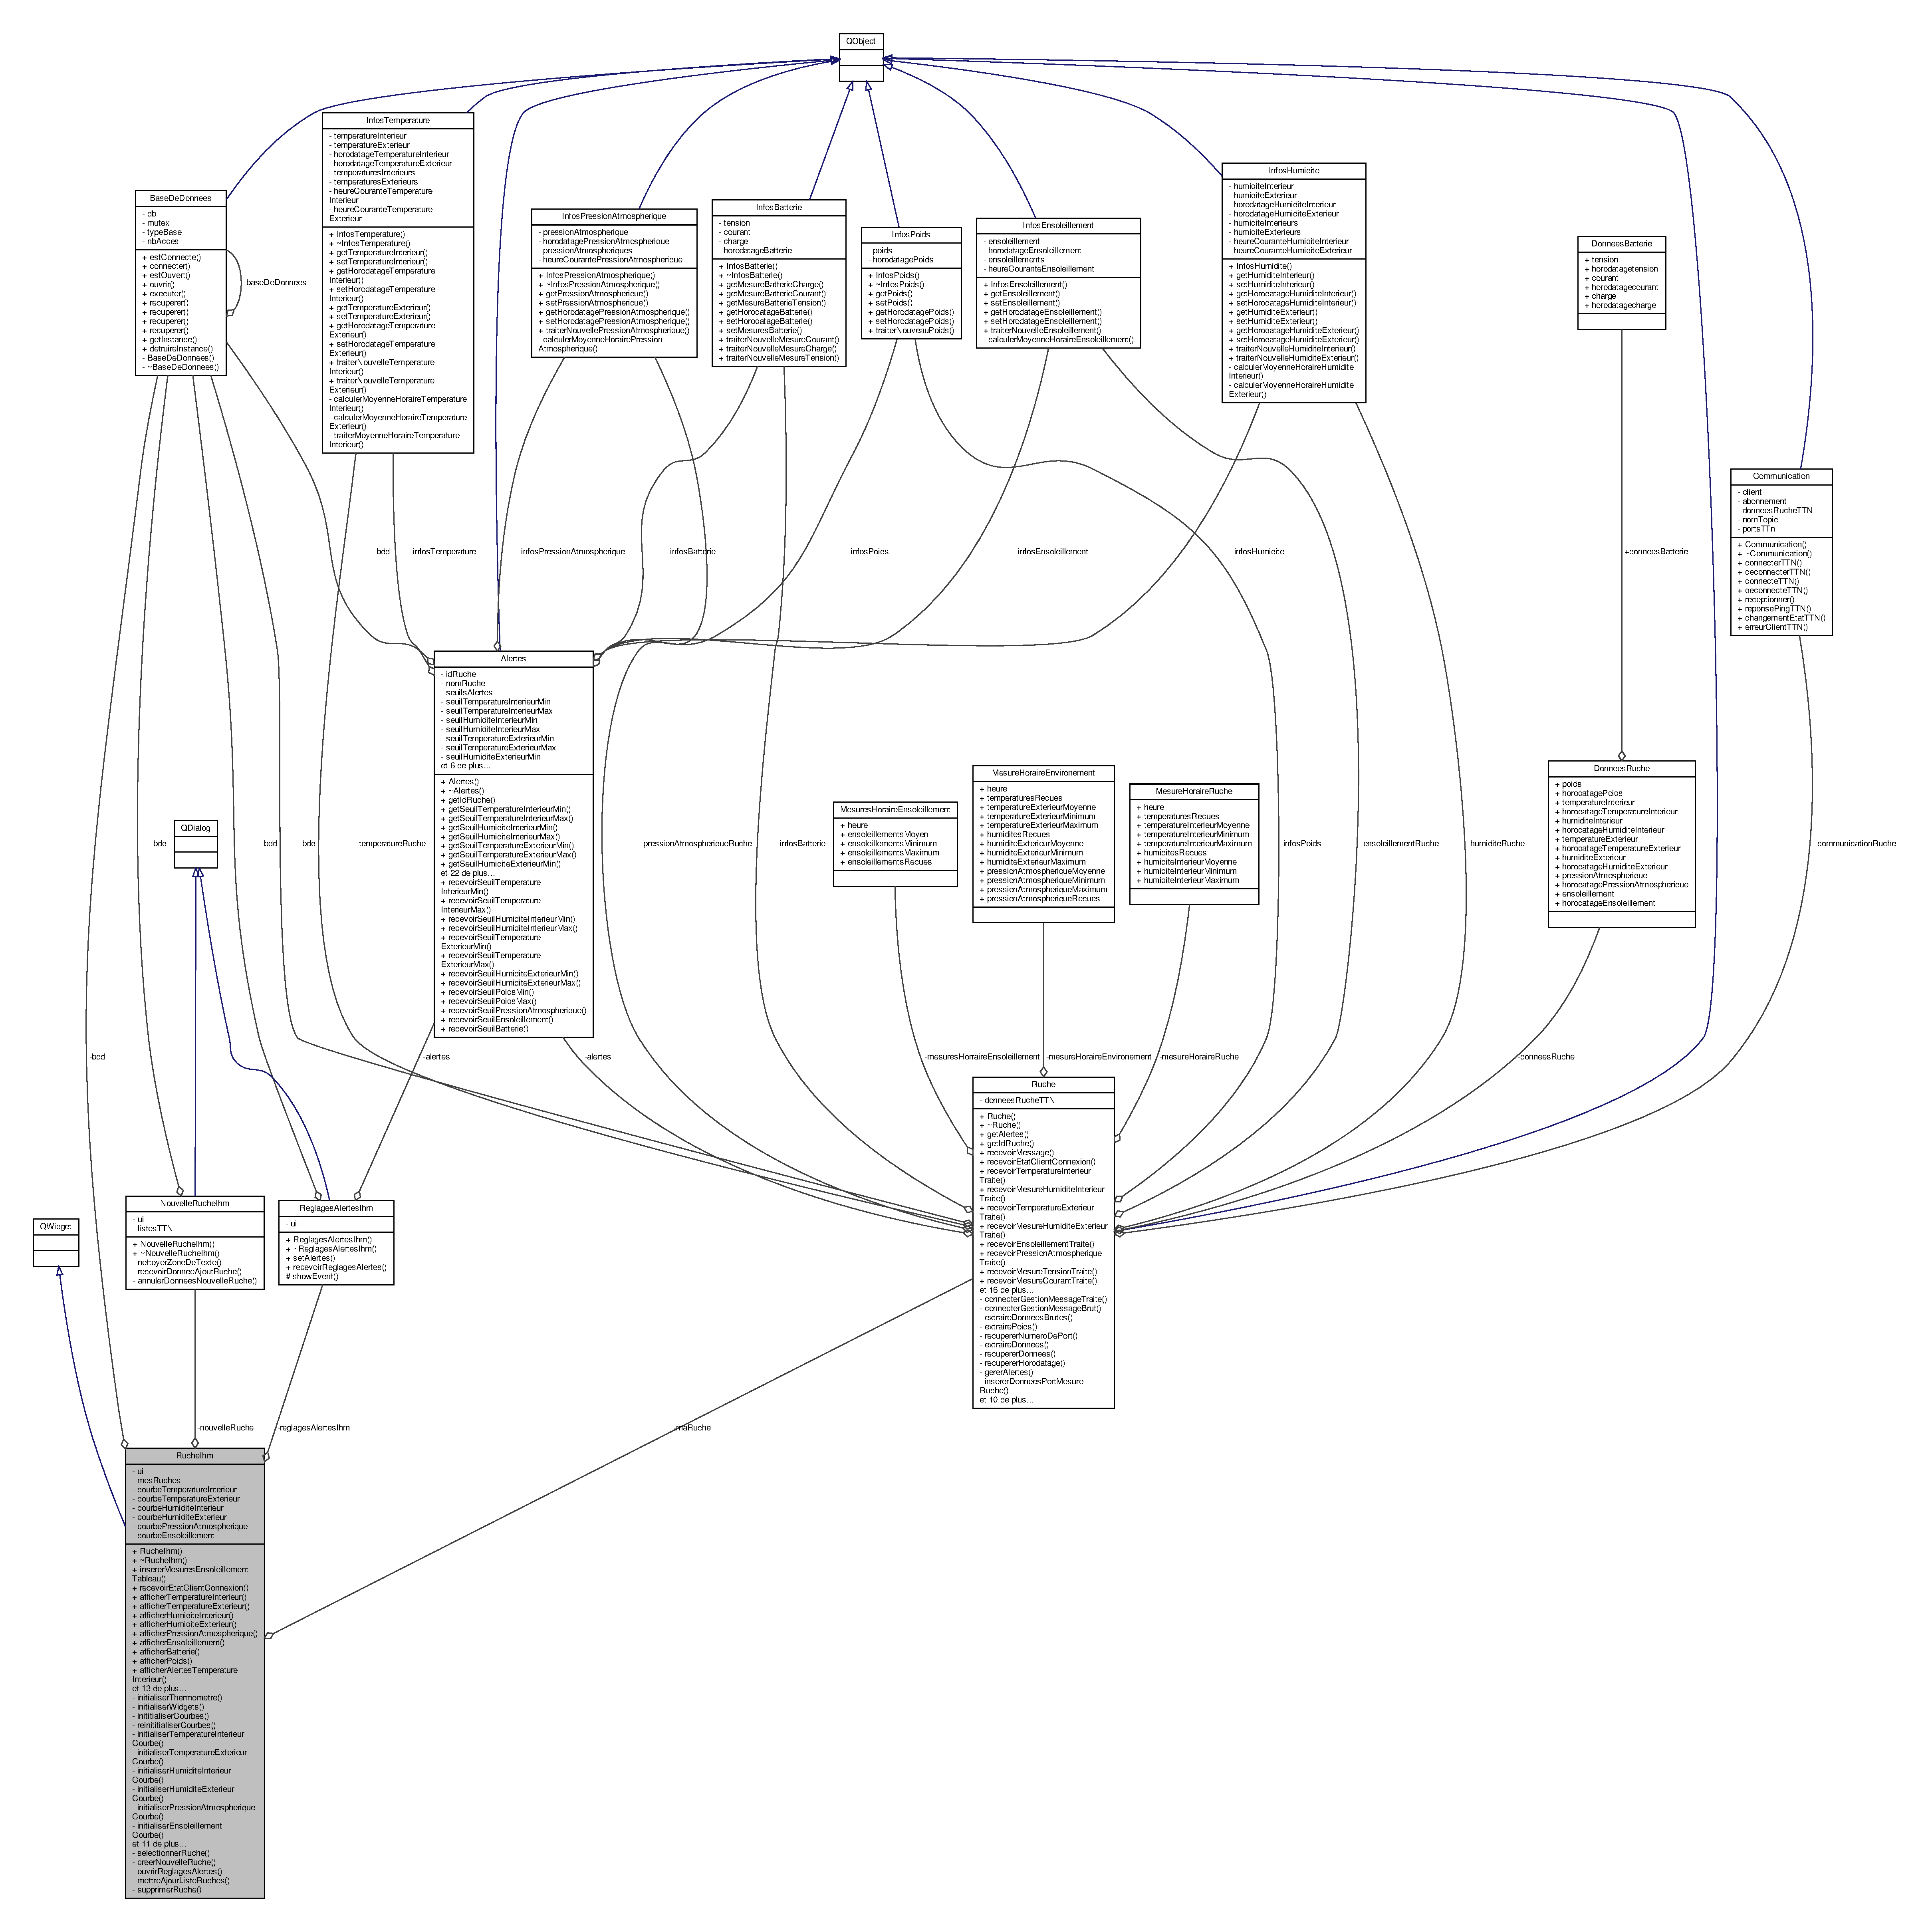
\includegraphics[width=350pt]{class_ruche_ihm__coll__graph}
\end{center}
\end{figure}
\subsubsection*{Connecteurs publics}
\begin{DoxyCompactItemize}
\item 
void \hyperlink{class_ruche_ihm_a3a3dae9de8c51344aa6e3463db9e6ad9}{recevoir\+Etat\+Client\+Connexion} (bool etat)
\item 
void \hyperlink{class_ruche_ihm_a4b8483705f88b46e253ef73068cd8f2e}{afficher\+Temperature\+Interieur} (double temperature\+Interieur, Q\+String horodatage)
\begin{DoxyCompactList}\small\item\em affiche temperature interieur à l\textquotesingle{}aide de widget graphique \end{DoxyCompactList}\item 
void \hyperlink{class_ruche_ihm_a63e3a82b98678d00d57748e80fe5258b}{afficher\+Temperature\+Exterieur} (double temperature\+Exterieur, Q\+String horodatage)
\begin{DoxyCompactList}\small\item\em affiche temperature exterieur à l\textquotesingle{}aide de widget graphique \end{DoxyCompactList}\item 
void \hyperlink{class_ruche_ihm_a4ab4b1ba1618a9aaf5bdb7f51df987aa}{afficher\+Humidite\+Interieur} (double humidite\+Interieur, Q\+String horodatage)
\begin{DoxyCompactList}\small\item\em affiche humidite interieur à l\textquotesingle{}aide de widget graphique \end{DoxyCompactList}\item 
void \hyperlink{class_ruche_ihm_a6381018a7dc88cb966d7bbc49515495e}{afficher\+Humidite\+Exterieur} (double humidite\+Exterieur, Q\+String horodatage)
\begin{DoxyCompactList}\small\item\em affiche humidite exterieur à l\textquotesingle{}aide de widget graphique \end{DoxyCompactList}\item 
void \hyperlink{class_ruche_ihm_ab38e4be7a1f39c862d7d8ab2ed3de98e}{afficher\+Pression\+Atmospherique} (double pression\+Atmospherique, Q\+String horodatage)
\begin{DoxyCompactList}\small\item\em affiche pression atmospherique à l\textquotesingle{}aide de widget graphique \end{DoxyCompactList}\item 
void \hyperlink{class_ruche_ihm_a8ee0041a209452e8e77f4a50adabff2b}{afficher\+Ensoleillement} (double ensoleillement, Q\+String horodatage)
\begin{DoxyCompactList}\small\item\em affiche l\textquotesingle{}ensoleillement à l\textquotesingle{}aide de widget graphique \end{DoxyCompactList}\item 
void \hyperlink{class_ruche_ihm_a3934082a49b22f4c6096d96887a11591}{afficher\+Batterie} (double charge, Q\+String horodatage)
\item 
void \hyperlink{class_ruche_ihm_a840ab51f951632e630f92e6c0b5ecc4d}{afficher\+Poids} (double poids, Q\+String horodatage)
\item 
void \hyperlink{class_ruche_ihm_af4848134f2bc17d9772f2408a068e9d8}{afficher\+Alertes\+Temperature\+Interieur} (\hyperlink{parametres_8h_aaa6de8207c94675264c90b10b613368d}{Seuils\+Alertes} type\+Alerte)
\item 
void \hyperlink{class_ruche_ihm_ada4be5a54f7fa57de6190d44e3cfcb82}{afficher\+Alertes\+Temperature\+Exterieur} (\hyperlink{parametres_8h_aaa6de8207c94675264c90b10b613368d}{Seuils\+Alertes} type\+Alerte)
\item 
void \hyperlink{class_ruche_ihm_abfe91b271dde97048bb218b04c9e167b}{afficher\+Alertes\+Humidite\+Interieur} (\hyperlink{parametres_8h_aaa6de8207c94675264c90b10b613368d}{Seuils\+Alertes} type\+Alerte)
\item 
void \hyperlink{class_ruche_ihm_a76b73e39e55443fc7b9bb773eac3321f}{afficher\+Alertes\+Humidite\+Exterieur} (\hyperlink{parametres_8h_aaa6de8207c94675264c90b10b613368d}{Seuils\+Alertes} type\+Alerte)
\item 
void \hyperlink{class_ruche_ihm_abea08b19d4f52f6767a8618bbc25d956}{afficher\+Alertes\+Pression\+Atmospherique} (\hyperlink{parametres_8h_aaa6de8207c94675264c90b10b613368d}{Seuils\+Alertes} type\+Alerte)
\item 
void \hyperlink{class_ruche_ihm_a641d05346e527c3386ed9df6a7e6fafc}{afficher\+Alertes\+Poids} (\hyperlink{parametres_8h_aaa6de8207c94675264c90b10b613368d}{Seuils\+Alertes} type\+Alerte)
\item 
void \hyperlink{class_ruche_ihm_aea5efc506f9825db2a4eb39a40d7eb18}{afficher\+Alertes\+Ensoleillement} (\hyperlink{parametres_8h_aaa6de8207c94675264c90b10b613368d}{Seuils\+Alertes} type\+Alerte, double mesure)
\item 
void \hyperlink{class_ruche_ihm_a5181062e21dc73908b660d97e9621fb6}{afficher\+Alertes\+Batterie} (\hyperlink{parametres_8h_aaa6de8207c94675264c90b10b613368d}{Seuils\+Alertes} type\+Alerte, double mesure)
\item 
void \hyperlink{class_ruche_ihm_a94bd98327a73a15aad1306fc31f53ce8}{afficher\+Mesures\+Journalieres\+Ruche} ()
\item 
void \hyperlink{class_ruche_ihm_a5ee5942435915ca134765f42ff4b9061}{afficher\+Mesures\+Journalieres\+Environement} ()
\item 
void \hyperlink{class_ruche_ihm_abc250d15e6782c522b3d6676e0ee032d}{afficher\+Mesures\+Journalieres\+Ensoleillement} ()
\item 
void \hyperlink{class_ruche_ihm_a7f66af552d9e7ba0d00437ff3b330706}{afficher\+Mesures\+Journalieres\+Selectionnee} ()
\item 
void \hyperlink{class_ruche_ihm_a47770b4dcfdaad34c66f6a8a5224a648}{afficher\+Localisation\+Passerelle} (Q\+String longitude, Q\+String latitude)
\item 
void \hyperlink{class_ruche_ihm_a382502aff2ab21abf60f05bf573477fd}{quitter} ()
\end{DoxyCompactItemize}
\subsubsection*{Signaux}
\begin{DoxyCompactItemize}
\item 
void \hyperlink{class_ruche_ihm_afd6ed2087307a9f8fc75ac1e7bcd8b22}{nouvelle\+Donnes\+Ruche} (Q\+String nom, Q\+String prenom, Q\+String email, Q\+String nom\+Topic)
\end{DoxyCompactItemize}
\subsubsection*{Fonctions membres publiques}
\begin{DoxyCompactItemize}
\item 
\hyperlink{class_ruche_ihm_a04c2544ba4e9cca6c38f553c32d63dee}{Ruche\+Ihm} (\hyperlink{class_q_widget}{Q\+Widget} $\ast$parent=0)
\begin{DoxyCompactList}\small\item\em Constructeur de la fenêtre principale. \end{DoxyCompactList}\item 
\hyperlink{class_ruche_ihm_a4c489bf18e8c9947a375322d03504419}{$\sim$\+Ruche\+Ihm} ()
\begin{DoxyCompactList}\small\item\em Destructeur de la fenêtre principale. \end{DoxyCompactList}\item 
void \hyperlink{class_ruche_ihm_a6830ca55859cc2899ae8eb51b112557b}{inserer\+Mesures\+Ensoleillement\+Tableau} (Q\+Vector$<$ Q\+String\+List $>$ mesures\+Journalieres\+Ensoleillement)
\end{DoxyCompactItemize}
\subsubsection*{Connecteurs privés}
\begin{DoxyCompactItemize}
\item 
void \hyperlink{class_ruche_ihm_a7324ae6ea574ccdad47783f466933157}{selectionner\+Ruche} (int numero\+Ruche)
\item 
void \hyperlink{class_ruche_ihm_a2a106515c13c06c51799432a1c2baa3b}{creer\+Nouvelle\+Ruche} ()
\begin{DoxyCompactList}\small\item\em creer une nouvelle ruche \end{DoxyCompactList}\item 
void \hyperlink{class_ruche_ihm_ab8db02641e73f348fd6162321a3765da}{ouvrir\+Reglages\+Alertes} ()
\item 
void \hyperlink{class_ruche_ihm_a77cb005fde7e2271e8721c23cef13b3e}{mettre\+Ajour\+Liste\+Ruches} ()
\item 
void \hyperlink{class_ruche_ihm_a85729b1ae4f3dfb5130eb45f5a426e3c}{supprimer\+Ruche} ()
\end{DoxyCompactItemize}
\subsubsection*{Fonctions membres privées}
\begin{DoxyCompactItemize}
\item 
void \hyperlink{class_ruche_ihm_afb64cca9f0e46c25487ef059a4826d49}{initialiser\+Thermometre} () const
\begin{DoxyCompactList}\small\item\em initialise les thermometres \end{DoxyCompactList}\item 
void \hyperlink{class_ruche_ihm_a98c493fcd2ef145a3d51ff84bbf8748e}{initialiser\+Widgets} ()
\item 
void \hyperlink{class_ruche_ihm_a4fe15b22538611ad9ffc4d807f8b78fd}{inititialiser\+Courbes} ()
\item 
void \hyperlink{class_ruche_ihm_a098911c0edd701f7892e3d140ebffbd9}{reinititialiser\+Courbes} ()
\item 
void \hyperlink{class_ruche_ihm_ad7297b44f6431c0b0c42f1b11d78ace1}{initialiser\+Temperature\+Interieur\+Courbe} ()
\item 
void \hyperlink{class_ruche_ihm_adb1039cc926ceb318c5d851f09d896c1}{initialiser\+Temperature\+Exterieur\+Courbe} ()
\item 
void \hyperlink{class_ruche_ihm_a0ab45ef3e5c512ff1bb4fcfaaa8872bd}{initialiser\+Humidite\+Interieur\+Courbe} ()
\item 
void \hyperlink{class_ruche_ihm_ab4bca9c5285c1e9added34ba374eaf84}{initialiser\+Humidite\+Exterieur\+Courbe} ()
\item 
void \hyperlink{class_ruche_ihm_ab070a28e49cab512d62ca449473706e5}{initialiser\+Pression\+Atmospherique\+Courbe} ()
\item 
void \hyperlink{class_ruche_ihm_a18936cec4b04cee55b582847a5f9c0d7}{initialiser\+Ensoleillement\+Courbe} ()
\item 
void \hyperlink{class_ruche_ihm_a0f44cb030202047fa9a364dfcbf9a13f}{Initialiser\+Marqueur\+Alerte\+Temperature\+Interieur} ()
\item 
void \hyperlink{class_ruche_ihm_a42785d6da8aca09d8becb6d500de8d9f}{initialiser\+Marqueur\+Alerte\+Humidite\+Interieur} ()
\item 
void \hyperlink{class_ruche_ihm_a410bcf0b7ac3ea7134af65d479802c48}{initialiser\+Marqueur\+Alerte\+Temperature\+Exterieur} ()
\item 
void \hyperlink{class_ruche_ihm_ae572f3f2b76e8c9b14a699d3e29422ee}{initialiser\+Marqueur\+Alerte\+Humidite\+Exterieur} ()
\item 
void \hyperlink{class_ruche_ihm_a87e4e8d783ea0f15d6304ed604c7ddaa}{initialiser\+Marqueur\+Alerte\+Pression} ()
\item 
void \hyperlink{class_ruche_ihm_a6d52dd904573d1bfc9551421ab53e8cc}{initialiser\+Marqueur\+Alerte\+Ensoleillement} ()
\item 
void \hyperlink{class_ruche_ihm_aa136c7922dc441aa86c00ec2d9c8b71c}{renitialiser\+Marqueurs} ()
\item 
void \hyperlink{class_ruche_ihm_afada4cd970c0e34c3fd62d63e5af7a88}{inserer\+Mesures\+Ruche\+Tableau} (Q\+Vector$<$ Q\+String\+List $>$ mesures\+Journalieres\+Ruche)
\item 
void \hyperlink{class_ruche_ihm_a7c292baed04f6240697afb6c6f894358}{inserer\+Mesures\+Environement\+Tableau} (Q\+Vector$<$ Q\+String\+List $>$ mesures\+Journalieres\+Environement)
\item 
void \hyperlink{class_ruche_ihm_a386868ba4e6e37b9d877fe3ab330e605}{effacer\+Tableau} ()
\item 
void \hyperlink{class_ruche_ihm_a348a76106f3072dd31a382c6025b8113}{deconnecter\+Signaux} ()
\begin{DoxyCompactList}\small\item\em Déconnecte les signaux. \end{DoxyCompactList}\end{DoxyCompactItemize}
\subsubsection*{Attributs privés}
\begin{DoxyCompactItemize}
\item 
Ui\+::\+Ruche\+Ihm $\ast$ \hyperlink{class_ruche_ihm_a64786058bd7f88ca2f1e9743bb27c25b}{ui}
\begin{DoxyCompactList}\small\item\em agrégation de la partie graphique de l\textquotesingle{}I\+HM \end{DoxyCompactList}\item 
\hyperlink{class_ruche}{Ruche} $\ast$ \hyperlink{class_ruche_ihm_a43a6b1fa31f4fba58d919daae3707b38}{ma\+Ruche}
\begin{DoxyCompactList}\small\item\em association de l\textquotesingle{}objet \hyperlink{class_ruche}{Ruche} \end{DoxyCompactList}\item 
\hyperlink{class_base_de_donnees}{Base\+De\+Donnees} $\ast$ \hyperlink{class_ruche_ihm_a0851936fe212e8d40538264f09749153}{bdd}
\begin{DoxyCompactList}\small\item\em agrégation de l\textquotesingle{}objet \hyperlink{class_base_de_donnees}{Base\+De\+Donnees} \end{DoxyCompactList}\item 
\hyperlink{class_nouvelle_ruche_ihm}{Nouvelle\+Ruche\+Ihm} $\ast$ \hyperlink{class_ruche_ihm_a3a27b7af842244c6db3623f5f256bed5}{nouvelle\+Ruche}
\begin{DoxyCompactList}\small\item\em l\textquotesingle{}ihm pour créer une nouvelle ruche \end{DoxyCompactList}\item 
\hyperlink{class_reglages_alertes_ihm}{Reglages\+Alertes\+Ihm} $\ast$ \hyperlink{class_ruche_ihm_a04068fbec978c2443f3baf08d4945929}{reglages\+Alertes\+Ihm}
\begin{DoxyCompactList}\small\item\em l\textquotesingle{}ihm pour régler les seuils d\textquotesingle{}une ruche \end{DoxyCompactList}\item 
Q\+Vector$<$ Q\+String\+List $>$ \hyperlink{class_ruche_ihm_ab7741fa67b19cbb2da7eb12c58cf83c1}{mes\+Ruches}
\begin{DoxyCompactList}\small\item\em tableau des informations sur les ruches \end{DoxyCompactList}\item 
Qwt\+Plot\+Curve $\ast$ \hyperlink{class_ruche_ihm_a6ce372c8df13bb78c09705432dcfcf58}{courbe\+Temperature\+Interieur}
\item 
Qwt\+Plot\+Curve $\ast$ \hyperlink{class_ruche_ihm_a68e72873a859840d3c91b147b8559118}{courbe\+Temperature\+Exterieur}
\item 
Qwt\+Plot\+Curve $\ast$ \hyperlink{class_ruche_ihm_a19a58f5841dc91eb7f84acd419f35678}{courbe\+Humidite\+Interieur}
\item 
Qwt\+Plot\+Curve $\ast$ \hyperlink{class_ruche_ihm_a0c9d769a392e3c1332f8908cd9d558eb}{courbe\+Humidite\+Exterieur}
\item 
Qwt\+Plot\+Curve $\ast$ \hyperlink{class_ruche_ihm_aa6685f1fc20aa4459eab3b0bb3c4d1ef}{courbe\+Pression\+Atmospherique}
\item 
Qwt\+Plot\+Curve $\ast$ \hyperlink{class_ruche_ihm_af160181f408b3a9519b97e67c810a0fd}{courbe\+Ensoleillement}
\end{DoxyCompactItemize}


\subsubsection{Description détaillée}
\begin{DoxyAuthor}{Auteur}
Florentin Mellah, Enzo Rossi
\end{DoxyAuthor}
\begin{DoxyVersion}{Version}
0.\+1 
\end{DoxyVersion}


\subsubsection{Documentation des constructeurs et destructeur}
\mbox{\Hypertarget{class_ruche_ihm_a04c2544ba4e9cca6c38f553c32d63dee}\label{class_ruche_ihm_a04c2544ba4e9cca6c38f553c32d63dee}} 
\index{Ruche\+Ihm@{Ruche\+Ihm}!Ruche\+Ihm@{Ruche\+Ihm}}
\index{Ruche\+Ihm@{Ruche\+Ihm}!Ruche\+Ihm@{Ruche\+Ihm}}
\paragraph{\texorpdfstring{Ruche\+Ihm()}{RucheIhm()}}
{\footnotesize\ttfamily Ruche\+Ihm\+::\+Ruche\+Ihm (\begin{DoxyParamCaption}\item[{\hyperlink{class_q_widget}{Q\+Widget} $\ast$}]{parent = {\ttfamily 0} }\end{DoxyParamCaption})\hspace{0.3cm}{\ttfamily [explicit]}}


\begin{DoxyParams}{Paramètres}
{\em parent} & \hyperlink{class_q_object}{Q\+Object} Adresse de l\textquotesingle{}objet Qt parent (0 = fenêtre principale) \\
\hline
\end{DoxyParams}


Références \hyperlink{class_ruche_ihm_a0851936fe212e8d40538264f09749153}{bdd}, \hyperlink{parametres_8h_a45f8f15b8f9a7ab4c2b219038ff64f6b}{B\+D\+D\+\_\+\+N\+O\+M\+B\+A\+SE}, \hyperlink{parametres_8h_ae2ded9166ed2553182545e97514c04f7}{B\+D\+D\+\_\+\+P\+A\+S\+S\+W\+O\+RD}, \hyperlink{parametres_8h_a423559dc987673b8aacaa9f369839bb0}{B\+D\+D\+\_\+\+S\+E\+R\+V\+E\+UR}, \hyperlink{parametres_8h_a88b5f5b81fa534553c68802384beff2c}{B\+D\+D\+\_\+\+U\+S\+E\+R\+N\+A\+ME}, \hyperlink{class_base_de_donnees_ac20da193923a9bfea5e38ee5a54820cd}{Base\+De\+Donnees\+::connecter()}, \hyperlink{class_ruche_ihm_a2a106515c13c06c51799432a1c2baa3b}{creer\+Nouvelle\+Ruche()}, \hyperlink{class_base_de_donnees_a00388973f3ec42e5c8e76e7af7e124b2}{Base\+De\+Donnees\+::est\+Connecte()}, \hyperlink{class_base_de_donnees_a80028aa2b6b4fbf30fb2e36357b7d3d3}{Base\+De\+Donnees\+::get\+Instance()}, \hyperlink{class_ruche_ihm_a98c493fcd2ef145a3d51ff84bbf8748e}{initialiser\+Widgets()}, \hyperlink{class_ruche_ihm_a4fe15b22538611ad9ffc4d807f8b78fd}{inititialiser\+Courbes()}, \hyperlink{class_ruche_ihm_a77cb005fde7e2271e8721c23cef13b3e}{mettre\+Ajour\+Liste\+Ruches()}, \hyperlink{class_ruche_ihm_a3a27b7af842244c6db3623f5f256bed5}{nouvelle\+Ruche}, \hyperlink{class_ruche_ihm_ab8db02641e73f348fd6162321a3765da}{ouvrir\+Reglages\+Alertes()}, \hyperlink{class_ruche_ihm_a382502aff2ab21abf60f05bf573477fd}{quitter()}, \hyperlink{class_ruche_ihm_a04068fbec978c2443f3baf08d4945929}{reglages\+Alertes\+Ihm}, \hyperlink{class_ruche_ihm_a7324ae6ea574ccdad47783f466933157}{selectionner\+Ruche()}, \hyperlink{class_ruche_ihm_a85729b1ae4f3dfb5130eb45f5a426e3c}{supprimer\+Ruche()}, et \hyperlink{class_ruche_ihm_a64786058bd7f88ca2f1e9743bb27c25b}{ui}.


\begin{DoxyCode}
00040                                   : \hyperlink{class_q_widget}{QWidget}(parent), \hyperlink{class_ruche_ihm_a64786058bd7f88ca2f1e9743bb27c25b}{ui}(\textcolor{keyword}{new} Ui::RucheIhm), 
      \hyperlink{class_ruche_ihm_a43a6b1fa31f4fba58d919daae3707b38}{maRuche}(0), \hyperlink{class_ruche_ihm_a0851936fe212e8d40538264f09749153}{bdd}(0), \hyperlink{class_ruche_ihm_a3a27b7af842244c6db3623f5f256bed5}{nouvelleRuche}(0), \hyperlink{class_ruche_ihm_a04068fbec978c2443f3baf08d4945929}{reglagesAlertesIhm}(0)
00041 \{
00042     qDebug()<< Q\_FUNC\_INFO;
00043     \textcolor{comment}{// Initialisation de l'IHM}
00044     \hyperlink{class_ruche_ihm_a64786058bd7f88ca2f1e9743bb27c25b}{ui}->setupUi(\textcolor{keyword}{this});
00045 
00046     \textcolor{comment}{// Initialisation des widgets}
00047     \hyperlink{class_ruche_ihm_a4fe15b22538611ad9ffc4d807f8b78fd}{inititialiserCourbes}();
00048     \hyperlink{class_ruche_ihm_a98c493fcd2ef145a3d51ff84bbf8748e}{initialiserWidgets}();
00049 
00050     \textcolor{comment}{// Affichage plein écran}
00051     \textcolor{keyword}{const} \textcolor{keywordtype}{int} width = qApp->desktop()->availableGeometry(\textcolor{keyword}{this}).width(); \textcolor{comment}{// ou : qApp->desktop()->width()}
00052     \textcolor{keyword}{const} \textcolor{keywordtype}{int} height = qApp->desktop()->availableGeometry(\textcolor{keyword}{this}).height(); \textcolor{comment}{// ou : qApp->desktop()->height()}
00053     resize(width, height);
00054 
00055     \textcolor{comment}{// Ajout de l'action Quitter}
00056     QAction *actionQuitter = \textcolor{keyword}{new} QAction(\textcolor{stringliteral}{"&Quitter"}, \textcolor{keyword}{this});
00057     actionQuitter->setShortcut(QKeySequence(QKeySequence::Quit)); \textcolor{comment}{// Ctrl+Q}
00058     addAction(actionQuitter);
00059 
00060     \textcolor{comment}{// Connexion signaux/slots}
00061     connect(actionQuitter, SIGNAL(triggered()), \textcolor{keyword}{this}, SLOT(\hyperlink{class_ruche_ihm_a382502aff2ab21abf60f05bf573477fd}{quitter}()));
00062     connect(\hyperlink{class_ruche_ihm_a64786058bd7f88ca2f1e9743bb27c25b}{ui}->comboBoxChoixRuche, SIGNAL(currentIndexChanged(\textcolor{keywordtype}{int})), \textcolor{keyword}{this}, SLOT(
      \hyperlink{class_ruche_ihm_a7324ae6ea574ccdad47783f466933157}{selectionnerRuche}(\textcolor{keywordtype}{int})));
00063     connect(\hyperlink{class_ruche_ihm_a64786058bd7f88ca2f1e9743bb27c25b}{ui}->pushButtonNouvelleRuche, SIGNAL(clicked()), \textcolor{keyword}{this}, SLOT(
      \hyperlink{class_ruche_ihm_a2a106515c13c06c51799432a1c2baa3b}{creerNouvelleRuche}()));
00064     connect(\hyperlink{class_ruche_ihm_a64786058bd7f88ca2f1e9743bb27c25b}{ui}->pushButtonReglages, SIGNAL(clicked()), \textcolor{keyword}{this}, SLOT(
      \hyperlink{class_ruche_ihm_ab8db02641e73f348fd6162321a3765da}{ouvrirReglagesAlertes}()));
00065     connect(\hyperlink{class_ruche_ihm_a64786058bd7f88ca2f1e9743bb27c25b}{ui}->pushButtonSuppressionRuche, SIGNAL(clicked()), \textcolor{keyword}{this}, SLOT(
      \hyperlink{class_ruche_ihm_a85729b1ae4f3dfb5130eb45f5a426e3c}{supprimerRuche}()));
00066 
00067     \hyperlink{class_ruche_ihm_a0851936fe212e8d40538264f09749153}{bdd} = \hyperlink{class_base_de_donnees_a80028aa2b6b4fbf30fb2e36357b7d3d3}{BaseDeDonnees::getInstance}();
00068     \textcolor{keywordflow}{if}(!\hyperlink{class_ruche_ihm_a0851936fe212e8d40538264f09749153}{bdd}->\hyperlink{class_base_de_donnees_a00388973f3ec42e5c8e76e7af7e124b2}{estConnecte}())
00069         \hyperlink{class_ruche_ihm_a0851936fe212e8d40538264f09749153}{bdd}->\hyperlink{class_base_de_donnees_ac20da193923a9bfea5e38ee5a54820cd}{connecter}(\hyperlink{parametres_8h_a45f8f15b8f9a7ab4c2b219038ff64f6b}{BDD\_NOMBASE}, \hyperlink{parametres_8h_a88b5f5b81fa534553c68802384beff2c}{BDD\_USERNAME}, 
      \hyperlink{parametres_8h_ae2ded9166ed2553182545e97514c04f7}{BDD\_PASSWORD}, \hyperlink{parametres_8h_a423559dc987673b8aacaa9f369839bb0}{BDD\_SERVEUR});
00070 
00071     \hyperlink{class_ruche_ihm_a3a27b7af842244c6db3623f5f256bed5}{nouvelleRuche} = \textcolor{keyword}{new} \hyperlink{class_nouvelle_ruche_ihm}{NouvelleRucheIhm}(\textcolor{keyword}{this});
00072     \hyperlink{class_ruche_ihm_a04068fbec978c2443f3baf08d4945929}{reglagesAlertesIhm} = \textcolor{keyword}{new} \hyperlink{class_reglages_alertes_ihm}{ReglagesAlertesIhm}(\textcolor{keyword}{this});
00073 
00074     \hyperlink{class_ruche_ihm_a77cb005fde7e2271e8721c23cef13b3e}{mettreAjourListeRuches}();
00075     \textcolor{comment}{//ui->comboBoxChoixRuche->setCurrentIndex(1);}
00076 \}
\end{DoxyCode}
\mbox{\Hypertarget{class_ruche_ihm_a4c489bf18e8c9947a375322d03504419}\label{class_ruche_ihm_a4c489bf18e8c9947a375322d03504419}} 
\index{Ruche\+Ihm@{Ruche\+Ihm}!````~Ruche\+Ihm@{$\sim$\+Ruche\+Ihm}}
\index{````~Ruche\+Ihm@{$\sim$\+Ruche\+Ihm}!Ruche\+Ihm@{Ruche\+Ihm}}
\paragraph{\texorpdfstring{$\sim$\+Ruche\+Ihm()}{~RucheIhm()}}
{\footnotesize\ttfamily Ruche\+Ihm\+::$\sim$\+Ruche\+Ihm (\begin{DoxyParamCaption}{ }\end{DoxyParamCaption})}



Références \hyperlink{class_base_de_donnees_a457401c0816b888c77ce915997545f4e}{Base\+De\+Donnees\+::detruire\+Instance()}, et \hyperlink{class_ruche_ihm_a64786058bd7f88ca2f1e9743bb27c25b}{ui}.


\begin{DoxyCode}
00085 \{
00086     \textcolor{keyword}{delete} \hyperlink{class_ruche_ihm_a64786058bd7f88ca2f1e9743bb27c25b}{ui};
00087     \hyperlink{class_base_de_donnees_a457401c0816b888c77ce915997545f4e}{BaseDeDonnees::detruireInstance}();
00088     qDebug()<< Q\_FUNC\_INFO;
00089 \}
\end{DoxyCode}


\subsubsection{Documentation des fonctions membres}
\mbox{\Hypertarget{class_ruche_ihm_a5181062e21dc73908b660d97e9621fb6}\label{class_ruche_ihm_a5181062e21dc73908b660d97e9621fb6}} 
\index{Ruche\+Ihm@{Ruche\+Ihm}!afficher\+Alertes\+Batterie@{afficher\+Alertes\+Batterie}}
\index{afficher\+Alertes\+Batterie@{afficher\+Alertes\+Batterie}!Ruche\+Ihm@{Ruche\+Ihm}}
\paragraph{\texorpdfstring{afficher\+Alertes\+Batterie}{afficherAlertesBatterie}}
{\footnotesize\ttfamily void Ruche\+Ihm\+::afficher\+Alertes\+Batterie (\begin{DoxyParamCaption}\item[{\hyperlink{parametres_8h_aaa6de8207c94675264c90b10b613368d}{Seuils\+Alertes}}]{type\+Alerte,  }\item[{double}]{mesure }\end{DoxyParamCaption})\hspace{0.3cm}{\ttfamily [slot]}}



Références \hyperlink{parametres_8h_a83a725fd153179a2bd97afcc8307737ba11c71364df2afd149875ebfe0238ef7e}{alerte\+Batterie}, \hyperlink{class_ruche_ihm_a0851936fe212e8d40538264f09749153}{bdd}, \hyperlink{parametres_8h_aaa6de8207c94675264c90b10b613368da5ac8ec3b54d90a07c6bb5a77ef971821}{bon}, \hyperlink{class_base_de_donnees_aa8de5f8f8bb17edc43f5c0ee33712081}{Base\+De\+Donnees\+::executer()}, \hyperlink{class_ruche_a9f2de5ef29557ec7a53d5e22df34d164}{Ruche\+::get\+Id\+Ruche()}, \hyperlink{class_ruche_ihm_a43a6b1fa31f4fba58d919daae3707b38}{ma\+Ruche}, \hyperlink{parametres_8h_aaa6de8207c94675264c90b10b613368da4257e2f8921856770c8266f55c937295}{trop\+Bas}, et \hyperlink{class_ruche_ihm_a64786058bd7f88ca2f1e9743bb27c25b}{ui}.



Référencé par \hyperlink{class_ruche_ihm_a348a76106f3072dd31a382c6025b8113}{deconnecter\+Signaux()}, et \hyperlink{class_ruche_ihm_a7324ae6ea574ccdad47783f466933157}{selectionner\+Ruche()}.


\begin{DoxyCode}
00635 \{
00636     qDebug() << Q\_FUNC\_INFO << \textcolor{stringliteral}{"SeuilsAlertes "} << typeAlerte << \textcolor{stringliteral}{"mesure "} << mesure;
00637 
00638     QString requete;
00639     QDateTime maintenant = QDateTime::currentDateTime();
00640 
00641     \textcolor{keywordflow}{if}(typeAlerte == \hyperlink{parametres_8h_aaa6de8207c94675264c90b10b613368da4257e2f8921856770c8266f55c937295}{tropBas} && mesure > 0 && mesure < 25)
00642     \{
00643         \hyperlink{class_ruche_ihm_a64786058bd7f88ca2f1e9743bb27c25b}{ui}->labelAlerteBatterie->setText(\textcolor{stringliteral}{"<strong>Batterie faible</strong>"});
00644         QPixmap imageBatterie(\textcolor{stringliteral}{":/images/images/batteryChargeMin.png"});
00645         \hyperlink{class_ruche_ihm_a64786058bd7f88ca2f1e9743bb27c25b}{ui}->labelAlerteImageBatterie->setPixmap(imageBatterie);
00646         requete = \textcolor{stringliteral}{"INSERT INTO Alertes (Alertes.idRuche, Alertes.idType, Alertes.Description,
       Alertes.Horodatage) VALUES ('"} + \hyperlink{class_ruche_ihm_a43a6b1fa31f4fba58d919daae3707b38}{maRuche}->\hyperlink{class_ruche_a9f2de5ef29557ec7a53d5e22df34d164}{getIdRuche}() + \textcolor{stringliteral}{"', '"} + QString::number(
      \hyperlink{parametres_8h_a83a725fd153179a2bd97afcc8307737ba11c71364df2afd149875ebfe0238ef7e}{alerteBatterie}) + \textcolor{stringliteral}{"', 'Batterie Faible','"} + maintenant.toString(\textcolor{stringliteral}{"yyyy-MM-dd  HH:mm:ss"}) + \textcolor{stringliteral}{"
      ')"};
00647         \hyperlink{class_ruche_ihm_a0851936fe212e8d40538264f09749153}{bdd}->\hyperlink{class_base_de_donnees_aa8de5f8f8bb17edc43f5c0ee33712081}{executer}(requete);
00648     \}
00649     \textcolor{keywordflow}{else} \textcolor{keywordflow}{if}(typeAlerte == \hyperlink{parametres_8h_aaa6de8207c94675264c90b10b613368da5ac8ec3b54d90a07c6bb5a77ef971821}{bon})
00650     \{
00651         \textcolor{keywordflow}{if}(mesure >= 75 && mesure <= 100)
00652         \{
00653             \hyperlink{class_ruche_ihm_a64786058bd7f88ca2f1e9743bb27c25b}{ui}->labelAlerteBatterie->setText(\textcolor{stringliteral}{"<strong>Batterie</strong>"});
00654             QPixmap imageBatterie(\textcolor{stringliteral}{":/images/images/batteryChargeMax.png"});
00655             \hyperlink{class_ruche_ihm_a64786058bd7f88ca2f1e9743bb27c25b}{ui}->labelAlerteImageBatterie->setPixmap(imageBatterie);
00656         \}
00657         \textcolor{keywordflow}{if}(mesure >= 50 && mesure < 75)
00658         \{
00659             \hyperlink{class_ruche_ihm_a64786058bd7f88ca2f1e9743bb27c25b}{ui}->labelAlerteBatterie->setText(\textcolor{stringliteral}{"<strong>Batterie</strong>"});
00660             QPixmap imageBatterie(\textcolor{stringliteral}{":/images/images/batteryChargeBonne.png"});
00661             \hyperlink{class_ruche_ihm_a64786058bd7f88ca2f1e9743bb27c25b}{ui}->labelAlerteImageBatterie->setPixmap(imageBatterie);
00662         \}
00663         \textcolor{keywordflow}{if}(mesure >= 25 && mesure < 50)
00664         \{
00665             \hyperlink{class_ruche_ihm_a64786058bd7f88ca2f1e9743bb27c25b}{ui}->labelAlerteBatterie->setText(\textcolor{stringliteral}{"<strong>Batterie</strong>"});
00666             QPixmap imageBatterie(\textcolor{stringliteral}{":/images/images/batteryChargeMoitie.png"});
00667             \hyperlink{class_ruche_ihm_a64786058bd7f88ca2f1e9743bb27c25b}{ui}->labelAlerteImageBatterie->setPixmap(imageBatterie);
00668         \}
00669     \}
00670 \}
\end{DoxyCode}
\mbox{\Hypertarget{class_ruche_ihm_aea5efc506f9825db2a4eb39a40d7eb18}\label{class_ruche_ihm_aea5efc506f9825db2a4eb39a40d7eb18}} 
\index{Ruche\+Ihm@{Ruche\+Ihm}!afficher\+Alertes\+Ensoleillement@{afficher\+Alertes\+Ensoleillement}}
\index{afficher\+Alertes\+Ensoleillement@{afficher\+Alertes\+Ensoleillement}!Ruche\+Ihm@{Ruche\+Ihm}}
\paragraph{\texorpdfstring{afficher\+Alertes\+Ensoleillement}{afficherAlertesEnsoleillement}}
{\footnotesize\ttfamily void Ruche\+Ihm\+::afficher\+Alertes\+Ensoleillement (\begin{DoxyParamCaption}\item[{\hyperlink{parametres_8h_aaa6de8207c94675264c90b10b613368d}{Seuils\+Alertes}}]{type\+Alerte,  }\item[{double}]{mesure }\end{DoxyParamCaption})\hspace{0.3cm}{\ttfamily [slot]}}



Références \hyperlink{parametres_8h_a83a725fd153179a2bd97afcc8307737ba256a82c8886c1902dc7a078868434f83}{alerte\+Ensoleillement}, \hyperlink{class_ruche_ihm_a0851936fe212e8d40538264f09749153}{bdd}, \hyperlink{parametres_8h_aaa6de8207c94675264c90b10b613368da5ac8ec3b54d90a07c6bb5a77ef971821}{bon}, \hyperlink{class_base_de_donnees_aa8de5f8f8bb17edc43f5c0ee33712081}{Base\+De\+Donnees\+::executer()}, \hyperlink{class_ruche_a9f2de5ef29557ec7a53d5e22df34d164}{Ruche\+::get\+Id\+Ruche()}, \hyperlink{class_ruche_ihm_a43a6b1fa31f4fba58d919daae3707b38}{ma\+Ruche}, \hyperlink{parametres_8h_aaa6de8207c94675264c90b10b613368dabc650d9700ae19f2696e6a6e3f9ab067}{trop\+Haut}, et \hyperlink{class_ruche_ihm_a64786058bd7f88ca2f1e9743bb27c25b}{ui}.



Référencé par \hyperlink{class_ruche_ihm_a348a76106f3072dd31a382c6025b8113}{deconnecter\+Signaux()}, et \hyperlink{class_ruche_ihm_a7324ae6ea574ccdad47783f466933157}{selectionner\+Ruche()}.


\begin{DoxyCode}
00589 \{
00590     qDebug() << Q\_FUNC\_INFO << \textcolor{stringliteral}{"SeuilsAlertes "} << typeAlerte << \textcolor{stringliteral}{"mesure "} << mesure;
00591 
00592     QString requete;
00593     QDateTime maintenant = QDateTime::currentDateTime();
00594 
00595     \textcolor{keywordflow}{if}(typeAlerte == \hyperlink{parametres_8h_aaa6de8207c94675264c90b10b613368dabc650d9700ae19f2696e6a6e3f9ab067}{tropHaut})
00596     \{
00597         \hyperlink{class_ruche_ihm_a64786058bd7f88ca2f1e9743bb27c25b}{ui}->labelAlerteEnsoleillement->setText(\textcolor{stringliteral}{"<strong>Ensoleillement Elevé</strong>"});
00598         QPixmap imageEnsoleillement(\textcolor{stringliteral}{":/images/images/alerteEnsoleillement.png"});
00599         \hyperlink{class_ruche_ihm_a64786058bd7f88ca2f1e9743bb27c25b}{ui}->labelAlerteImageEnsoleillement->setPixmap(imageEnsoleillement);
00600         requete = \textcolor{stringliteral}{"INSERT INTO Alertes (Alertes.idRuche, Alertes.idType, Alertes.Description,
       Alertes.Horodatage) VALUES ('"} + \hyperlink{class_ruche_ihm_a43a6b1fa31f4fba58d919daae3707b38}{maRuche}->\hyperlink{class_ruche_a9f2de5ef29557ec7a53d5e22df34d164}{getIdRuche}() + \textcolor{stringliteral}{"', '"} + QString::number(
      \hyperlink{parametres_8h_a83a725fd153179a2bd97afcc8307737ba256a82c8886c1902dc7a078868434f83}{alerteEnsoleillement}) + \textcolor{stringliteral}{"', 'Ensoleillement Elevé','"} + maintenant.toString(\textcolor{stringliteral}{"yyyy-MM-dd
        HH:mm:ss"}) + \textcolor{stringliteral}{"')"};
00601         \hyperlink{class_ruche_ihm_a0851936fe212e8d40538264f09749153}{bdd}->\hyperlink{class_base_de_donnees_aa8de5f8f8bb17edc43f5c0ee33712081}{executer}(requete);
00602     \}
00603     \textcolor{keywordflow}{else} \textcolor{keywordflow}{if}(typeAlerte == \hyperlink{parametres_8h_aaa6de8207c94675264c90b10b613368da5ac8ec3b54d90a07c6bb5a77ef971821}{bon})
00604     \{
00605         \textcolor{keywordflow}{if}(mesure >=800 && mesure <= 1800)
00606         \{
00607             \hyperlink{class_ruche_ihm_a64786058bd7f88ca2f1e9743bb27c25b}{ui}->labelAlerteEnsoleillement->setText(\textcolor{stringliteral}{"<strong>Ensoleillé</strong>"});
00608             QPixmap imageEnsoleillement(\textcolor{stringliteral}{":/images/images/soleil.png"});
00609             \hyperlink{class_ruche_ihm_a64786058bd7f88ca2f1e9743bb27c25b}{ui}->labelAlerteImageEnsoleillement->setPixmap(imageEnsoleillement);
00610         \}
00611         \textcolor{keywordflow}{if}(mesure >= 400 && mesure < 800)
00612         \{
00613             \hyperlink{class_ruche_ihm_a64786058bd7f88ca2f1e9743bb27c25b}{ui}->labelAlerteEnsoleillement->setText(\textcolor{stringliteral}{"<strong>Ensoleillé dans l'ensemble</strong>"});
00614             QPixmap imageEnsoleillement(\textcolor{stringliteral}{":/images/images/soleilCouvert.png"});
00615             \hyperlink{class_ruche_ihm_a64786058bd7f88ca2f1e9743bb27c25b}{ui}->labelAlerteImageEnsoleillement->setPixmap(imageEnsoleillement);
00616         \}
00617         \textcolor{keywordflow}{if}(mesure > 40 && mesure < 400)
00618         \{
00619             \hyperlink{class_ruche_ihm_a64786058bd7f88ca2f1e9743bb27c25b}{ui}->labelAlerteEnsoleillement->setText(\textcolor{stringliteral}{"<strong>Couvert</strong>"});
00620             QPixmap imageEnsoleillement(\textcolor{stringliteral}{":/images/images/nuageux.png"});
00621             \hyperlink{class_ruche_ihm_a64786058bd7f88ca2f1e9743bb27c25b}{ui}->labelAlerteImageEnsoleillement->setPixmap(imageEnsoleillement);
00622             requete = \textcolor{stringliteral}{"INSERT INTO Alertes (Alertes.idRuche, Alertes.idType, Alertes.Description,
       Alertes.Horodatage) VALUES ('"} + \hyperlink{class_ruche_ihm_a43a6b1fa31f4fba58d919daae3707b38}{maRuche}->\hyperlink{class_ruche_a9f2de5ef29557ec7a53d5e22df34d164}{getIdRuche}() + \textcolor{stringliteral}{"', '"} + QString::number(
      \hyperlink{parametres_8h_a83a725fd153179a2bd97afcc8307737ba256a82c8886c1902dc7a078868434f83}{alerteEnsoleillement}) + \textcolor{stringliteral}{"', 'Couvert','"} + maintenant.toString(\textcolor{stringliteral}{"yyyy-MM-dd  HH:mm:ss"}) 
      + \textcolor{stringliteral}{"')"};
00623             \hyperlink{class_ruche_ihm_a0851936fe212e8d40538264f09749153}{bdd}->\hyperlink{class_base_de_donnees_aa8de5f8f8bb17edc43f5c0ee33712081}{executer}(requete);
00624         \}
00625         \textcolor{keywordflow}{if}(mesure <= 40)
00626         \{
00627             \hyperlink{class_ruche_ihm_a64786058bd7f88ca2f1e9743bb27c25b}{ui}->labelAlerteEnsoleillement->setText(\textcolor{stringliteral}{"<strong>Nuit</strong>"});
00628             QPixmap imageEnsoleillement(\textcolor{stringliteral}{":/images/images/moon.png"});
00629             \hyperlink{class_ruche_ihm_a64786058bd7f88ca2f1e9743bb27c25b}{ui}->labelAlerteImageEnsoleillement->setPixmap(imageEnsoleillement);
00630         \}
00631     \}
00632 \}
\end{DoxyCode}
\mbox{\Hypertarget{class_ruche_ihm_a76b73e39e55443fc7b9bb773eac3321f}\label{class_ruche_ihm_a76b73e39e55443fc7b9bb773eac3321f}} 
\index{Ruche\+Ihm@{Ruche\+Ihm}!afficher\+Alertes\+Humidite\+Exterieur@{afficher\+Alertes\+Humidite\+Exterieur}}
\index{afficher\+Alertes\+Humidite\+Exterieur@{afficher\+Alertes\+Humidite\+Exterieur}!Ruche\+Ihm@{Ruche\+Ihm}}
\paragraph{\texorpdfstring{afficher\+Alertes\+Humidite\+Exterieur}{afficherAlertesHumiditeExterieur}}
{\footnotesize\ttfamily void Ruche\+Ihm\+::afficher\+Alertes\+Humidite\+Exterieur (\begin{DoxyParamCaption}\item[{\hyperlink{parametres_8h_aaa6de8207c94675264c90b10b613368d}{Seuils\+Alertes}}]{type\+Alerte }\end{DoxyParamCaption})\hspace{0.3cm}{\ttfamily [slot]}}



Références \hyperlink{parametres_8h_a83a725fd153179a2bd97afcc8307737bacda66fabe33c8c197f8ff098a952fca3}{alerte\+Humidite\+Exterieur}, \hyperlink{class_ruche_ihm_a0851936fe212e8d40538264f09749153}{bdd}, \hyperlink{parametres_8h_aaa6de8207c94675264c90b10b613368da5ac8ec3b54d90a07c6bb5a77ef971821}{bon}, \hyperlink{class_base_de_donnees_aa8de5f8f8bb17edc43f5c0ee33712081}{Base\+De\+Donnees\+::executer()}, \hyperlink{class_ruche_a9f2de5ef29557ec7a53d5e22df34d164}{Ruche\+::get\+Id\+Ruche()}, \hyperlink{class_ruche_ihm_a43a6b1fa31f4fba58d919daae3707b38}{ma\+Ruche}, \hyperlink{parametres_8h_aaa6de8207c94675264c90b10b613368da4257e2f8921856770c8266f55c937295}{trop\+Bas}, \hyperlink{parametres_8h_aaa6de8207c94675264c90b10b613368dabc650d9700ae19f2696e6a6e3f9ab067}{trop\+Haut}, et \hyperlink{class_ruche_ihm_a64786058bd7f88ca2f1e9743bb27c25b}{ui}.



Référencé par \hyperlink{class_ruche_ihm_a348a76106f3072dd31a382c6025b8113}{deconnecter\+Signaux()}, et \hyperlink{class_ruche_ihm_a7324ae6ea574ccdad47783f466933157}{selectionner\+Ruche()}.


\begin{DoxyCode}
00498 \{
00499     \{
00500         qDebug() << Q\_FUNC\_INFO << \textcolor{stringliteral}{"SeuilsAlertes "} << typeAlerte;
00501         QString requete;
00502         QDateTime maintenant = QDateTime::currentDateTime();
00503 
00504         \textcolor{keywordflow}{if}(typeAlerte == \hyperlink{parametres_8h_aaa6de8207c94675264c90b10b613368dabc650d9700ae19f2696e6a6e3f9ab067}{tropHaut})
00505          \{
00506             \hyperlink{class_ruche_ihm_a64786058bd7f88ca2f1e9743bb27c25b}{ui}->labelAlerteHumiditeExterieur->setText(\textcolor{stringliteral}{"<strong>Humidité Ext. Elevée</strong>"});
00507             QPixmap imageHumiditeExterieur(\textcolor{stringliteral}{":/images/images/humidityHaute.png"});
00508             \hyperlink{class_ruche_ihm_a64786058bd7f88ca2f1e9743bb27c25b}{ui}->labelAlerteImageHumiditeExterieur->setPixmap(imageHumiditeExterieur);
00509             requete = \textcolor{stringliteral}{"INSERT INTO Alertes (Alertes.idRuche, Alertes.idType, Alertes.Description,
       Alertes.Horodatage) VALUES ('"} + \hyperlink{class_ruche_ihm_a43a6b1fa31f4fba58d919daae3707b38}{maRuche}->\hyperlink{class_ruche_a9f2de5ef29557ec7a53d5e22df34d164}{getIdRuche}() + \textcolor{stringliteral}{"', '"} + QString::number(
      \hyperlink{parametres_8h_a83a725fd153179a2bd97afcc8307737bacda66fabe33c8c197f8ff098a952fca3}{alerteHumiditeExterieur}) + \textcolor{stringliteral}{"', 'Humidité Extérieur Elevée','"} + maintenant.toString(\textcolor{stringliteral}{
      "yyyy-MM-dd  HH:mm:ss"}) + \textcolor{stringliteral}{"')"};
00510             \hyperlink{class_ruche_ihm_a0851936fe212e8d40538264f09749153}{bdd}->\hyperlink{class_base_de_donnees_aa8de5f8f8bb17edc43f5c0ee33712081}{executer}(requete);
00511          \}
00512          \textcolor{keywordflow}{else} \textcolor{keywordflow}{if}(typeAlerte == \hyperlink{parametres_8h_aaa6de8207c94675264c90b10b613368da4257e2f8921856770c8266f55c937295}{tropBas})
00513          \{
00514             \hyperlink{class_ruche_ihm_a64786058bd7f88ca2f1e9743bb27c25b}{ui}->labelAlerteHumiditeExterieur->setText(\textcolor{stringliteral}{"<strong>Humidité Ext. Basse</strong>"});
00515             QPixmap imageHumiditeExterieur(\textcolor{stringliteral}{":/images/images/humidityHaute.png"});
00516             \hyperlink{class_ruche_ihm_a64786058bd7f88ca2f1e9743bb27c25b}{ui}->labelAlerteImageHumiditeExterieur->setPixmap(imageHumiditeExterieur);
00517             requete = \textcolor{stringliteral}{"INSERT INTO Alertes (Alertes.idRuche, Alertes.idType, Alertes.Description,
       Alertes.Horodatage) VALUES ('"} + \hyperlink{class_ruche_ihm_a43a6b1fa31f4fba58d919daae3707b38}{maRuche}->\hyperlink{class_ruche_a9f2de5ef29557ec7a53d5e22df34d164}{getIdRuche}() + \textcolor{stringliteral}{"', '"} + QString::number(
      \hyperlink{parametres_8h_a83a725fd153179a2bd97afcc8307737bacda66fabe33c8c197f8ff098a952fca3}{alerteHumiditeExterieur}) + \textcolor{stringliteral}{"', 'Humidité Extérieur Basse','"} + maintenant.toString(\textcolor{stringliteral}{"
      yyyy-MM-dd  HH:mm:ss"}) + \textcolor{stringliteral}{"')"};
00518             \hyperlink{class_ruche_ihm_a0851936fe212e8d40538264f09749153}{bdd}->\hyperlink{class_base_de_donnees_aa8de5f8f8bb17edc43f5c0ee33712081}{executer}(requete);
00519          \}
00520          \textcolor{keywordflow}{else} \textcolor{keywordflow}{if}(typeAlerte == \hyperlink{parametres_8h_aaa6de8207c94675264c90b10b613368da5ac8ec3b54d90a07c6bb5a77ef971821}{bon})
00521          \{
00522             \hyperlink{class_ruche_ihm_a64786058bd7f88ca2f1e9743bb27c25b}{ui}->labelAlerteHumiditeExterieur->setText(\textcolor{stringliteral}{"<strong>Humidité Ext. Normale</strong>"});
00523             QPixmap imageHumiditeExterieur(\textcolor{stringliteral}{":/images/images/humiditeNormal.png"});
00524             \hyperlink{class_ruche_ihm_a64786058bd7f88ca2f1e9743bb27c25b}{ui}->labelAlerteImageHumiditeExterieur->setPixmap(imageHumiditeExterieur);
00525          \}
00526     \}
00527 \}
\end{DoxyCode}
\mbox{\Hypertarget{class_ruche_ihm_abfe91b271dde97048bb218b04c9e167b}\label{class_ruche_ihm_abfe91b271dde97048bb218b04c9e167b}} 
\index{Ruche\+Ihm@{Ruche\+Ihm}!afficher\+Alertes\+Humidite\+Interieur@{afficher\+Alertes\+Humidite\+Interieur}}
\index{afficher\+Alertes\+Humidite\+Interieur@{afficher\+Alertes\+Humidite\+Interieur}!Ruche\+Ihm@{Ruche\+Ihm}}
\paragraph{\texorpdfstring{afficher\+Alertes\+Humidite\+Interieur}{afficherAlertesHumiditeInterieur}}
{\footnotesize\ttfamily void Ruche\+Ihm\+::afficher\+Alertes\+Humidite\+Interieur (\begin{DoxyParamCaption}\item[{\hyperlink{parametres_8h_aaa6de8207c94675264c90b10b613368d}{Seuils\+Alertes}}]{type\+Alerte }\end{DoxyParamCaption})\hspace{0.3cm}{\ttfamily [slot]}}



Références \hyperlink{parametres_8h_a83a725fd153179a2bd97afcc8307737bac0e80b2d9b7f04033abc44ebcf61883a}{alerte\+Humidite\+Interieur}, \hyperlink{class_ruche_ihm_a0851936fe212e8d40538264f09749153}{bdd}, \hyperlink{parametres_8h_aaa6de8207c94675264c90b10b613368da5ac8ec3b54d90a07c6bb5a77ef971821}{bon}, \hyperlink{class_base_de_donnees_aa8de5f8f8bb17edc43f5c0ee33712081}{Base\+De\+Donnees\+::executer()}, \hyperlink{class_ruche_a9f2de5ef29557ec7a53d5e22df34d164}{Ruche\+::get\+Id\+Ruche()}, \hyperlink{class_ruche_ihm_a43a6b1fa31f4fba58d919daae3707b38}{ma\+Ruche}, \hyperlink{parametres_8h_aaa6de8207c94675264c90b10b613368da4257e2f8921856770c8266f55c937295}{trop\+Bas}, \hyperlink{parametres_8h_aaa6de8207c94675264c90b10b613368dabc650d9700ae19f2696e6a6e3f9ab067}{trop\+Haut}, et \hyperlink{class_ruche_ihm_a64786058bd7f88ca2f1e9743bb27c25b}{ui}.



Référencé par \hyperlink{class_ruche_ihm_a348a76106f3072dd31a382c6025b8113}{deconnecter\+Signaux()}, et \hyperlink{class_ruche_ihm_a7324ae6ea574ccdad47783f466933157}{selectionner\+Ruche()}.


\begin{DoxyCode}
00468 \{
00469     qDebug() << Q\_FUNC\_INFO << \textcolor{stringliteral}{"SeuilsAlertes "} << typeAlerte;
00470     QString requete;
00471     QDateTime maintenant = QDateTime::currentDateTime();
00472 
00473     \textcolor{keywordflow}{if}(typeAlerte == \hyperlink{parametres_8h_aaa6de8207c94675264c90b10b613368dabc650d9700ae19f2696e6a6e3f9ab067}{tropHaut})
00474      \{
00475         \hyperlink{class_ruche_ihm_a64786058bd7f88ca2f1e9743bb27c25b}{ui}->labelAlerteHumiditeInterieur->setText(\textcolor{stringliteral}{"<strong>Humidité Int. Elevée</strong>"});
00476         QPixmap imageHumiditeInterieur(\textcolor{stringliteral}{":/images/images/humidityHaute.png"});
00477         \hyperlink{class_ruche_ihm_a64786058bd7f88ca2f1e9743bb27c25b}{ui}->labelAlerteImageHumiditeInterieur->setPixmap(imageHumiditeInterieur);
00478         requete = \textcolor{stringliteral}{"INSERT INTO Alertes (Alertes.idRuche, Alertes.idType, Alertes.Description,
       Alertes.Horodatage) VALUES ('"} + \hyperlink{class_ruche_ihm_a43a6b1fa31f4fba58d919daae3707b38}{maRuche}->\hyperlink{class_ruche_a9f2de5ef29557ec7a53d5e22df34d164}{getIdRuche}() + \textcolor{stringliteral}{"', '"} + QString::number(
      \hyperlink{parametres_8h_a83a725fd153179a2bd97afcc8307737bac0e80b2d9b7f04033abc44ebcf61883a}{alerteHumiditeInterieur}) + \textcolor{stringliteral}{"', 'Humidité Intérieur Elevée','"} + maintenant.toString(\textcolor{stringliteral}{
      "yyyy-MM-dd  HH:mm:ss"}) + \textcolor{stringliteral}{"')"};
00479         \hyperlink{class_ruche_ihm_a0851936fe212e8d40538264f09749153}{bdd}->\hyperlink{class_base_de_donnees_aa8de5f8f8bb17edc43f5c0ee33712081}{executer}(requete);
00480      \}
00481      \textcolor{keywordflow}{else} \textcolor{keywordflow}{if}(typeAlerte == \hyperlink{parametres_8h_aaa6de8207c94675264c90b10b613368da4257e2f8921856770c8266f55c937295}{tropBas})
00482      \{
00483         \hyperlink{class_ruche_ihm_a64786058bd7f88ca2f1e9743bb27c25b}{ui}->labelAlerteHumiditeInterieur->setText(\textcolor{stringliteral}{"<strong>Humidité Int. Basse</strong>"});
00484         QPixmap imageHumiditeInterieur(\textcolor{stringliteral}{":/images/images/humidityHaute.png"});
00485         \hyperlink{class_ruche_ihm_a64786058bd7f88ca2f1e9743bb27c25b}{ui}->labelAlerteImageHumiditeInterieur->setPixmap(imageHumiditeInterieur);
00486         requete = \textcolor{stringliteral}{"INSERT INTO Alertes (Alertes.idRuche, Alertes.idType, Alertes.Description,
       Alertes.Horodatage) VALUES ('"} + \hyperlink{class_ruche_ihm_a43a6b1fa31f4fba58d919daae3707b38}{maRuche}->\hyperlink{class_ruche_a9f2de5ef29557ec7a53d5e22df34d164}{getIdRuche}() + \textcolor{stringliteral}{"', '"} + QString::number(
      \hyperlink{parametres_8h_a83a725fd153179a2bd97afcc8307737bac0e80b2d9b7f04033abc44ebcf61883a}{alerteHumiditeInterieur}) + \textcolor{stringliteral}{"', 'Humidité Intérieur Basse','"} + maintenant.toString(\textcolor{stringliteral}{"
      yyyy-MM-dd  HH:mm:ss"}) + \textcolor{stringliteral}{"')"};
00487         \hyperlink{class_ruche_ihm_a0851936fe212e8d40538264f09749153}{bdd}->\hyperlink{class_base_de_donnees_aa8de5f8f8bb17edc43f5c0ee33712081}{executer}(requete);
00488      \}
00489      \textcolor{keywordflow}{else} \textcolor{keywordflow}{if}(typeAlerte == \hyperlink{parametres_8h_aaa6de8207c94675264c90b10b613368da5ac8ec3b54d90a07c6bb5a77ef971821}{bon})
00490      \{
00491         \hyperlink{class_ruche_ihm_a64786058bd7f88ca2f1e9743bb27c25b}{ui}->labelAlerteHumiditeInterieur->setText(\textcolor{stringliteral}{"<strong>Humidité Int. Normale</strong>"});
00492         QPixmap imageHumiditeInterieur(\textcolor{stringliteral}{":/images/images/humiditeNormal.png"});
00493         \hyperlink{class_ruche_ihm_a64786058bd7f88ca2f1e9743bb27c25b}{ui}->labelAlerteImageHumiditeInterieur->setPixmap(imageHumiditeInterieur);
00494      \}
00495 \}
\end{DoxyCode}
\mbox{\Hypertarget{class_ruche_ihm_a641d05346e527c3386ed9df6a7e6fafc}\label{class_ruche_ihm_a641d05346e527c3386ed9df6a7e6fafc}} 
\index{Ruche\+Ihm@{Ruche\+Ihm}!afficher\+Alertes\+Poids@{afficher\+Alertes\+Poids}}
\index{afficher\+Alertes\+Poids@{afficher\+Alertes\+Poids}!Ruche\+Ihm@{Ruche\+Ihm}}
\paragraph{\texorpdfstring{afficher\+Alertes\+Poids}{afficherAlertesPoids}}
{\footnotesize\ttfamily void Ruche\+Ihm\+::afficher\+Alertes\+Poids (\begin{DoxyParamCaption}\item[{\hyperlink{parametres_8h_aaa6de8207c94675264c90b10b613368d}{Seuils\+Alertes}}]{type\+Alerte }\end{DoxyParamCaption})\hspace{0.3cm}{\ttfamily [slot]}}



Références \hyperlink{parametres_8h_a83a725fd153179a2bd97afcc8307737ba130a82230092934eb515b95603d12956}{alerte\+Poids}, \hyperlink{class_ruche_ihm_a0851936fe212e8d40538264f09749153}{bdd}, \hyperlink{parametres_8h_aaa6de8207c94675264c90b10b613368da5ac8ec3b54d90a07c6bb5a77ef971821}{bon}, \hyperlink{class_base_de_donnees_aa8de5f8f8bb17edc43f5c0ee33712081}{Base\+De\+Donnees\+::executer()}, \hyperlink{class_ruche_a9f2de5ef29557ec7a53d5e22df34d164}{Ruche\+::get\+Id\+Ruche()}, \hyperlink{class_ruche_ihm_a43a6b1fa31f4fba58d919daae3707b38}{ma\+Ruche}, \hyperlink{parametres_8h_aaa6de8207c94675264c90b10b613368da4257e2f8921856770c8266f55c937295}{trop\+Bas}, \hyperlink{parametres_8h_aaa6de8207c94675264c90b10b613368dabc650d9700ae19f2696e6a6e3f9ab067}{trop\+Haut}, et \hyperlink{class_ruche_ihm_a64786058bd7f88ca2f1e9743bb27c25b}{ui}.



Référencé par \hyperlink{class_ruche_ihm_a348a76106f3072dd31a382c6025b8113}{deconnecter\+Signaux()}, et \hyperlink{class_ruche_ihm_a7324ae6ea574ccdad47783f466933157}{selectionner\+Ruche()}.


\begin{DoxyCode}
00560 \{
00561     qDebug() << Q\_FUNC\_INFO << \textcolor{stringliteral}{"SeuilsAlertes "} << typeAlerte;
00562     QString requete;
00563     QDateTime maintenant = QDateTime::currentDateTime();
00564 
00565     \textcolor{keywordflow}{if}(typeAlerte == \hyperlink{parametres_8h_aaa6de8207c94675264c90b10b613368dabc650d9700ae19f2696e6a6e3f9ab067}{tropHaut})
00566     \{
00567         \hyperlink{class_ruche_ihm_a64786058bd7f88ca2f1e9743bb27c25b}{ui}->labelAlertePoids->setText(\textcolor{stringliteral}{"<strong>Poids Elevé</strong>"});
00568         QPixmap imagePoids(\textcolor{stringliteral}{":/images/images/poidsAlerte.png"});
00569         \hyperlink{class_ruche_ihm_a64786058bd7f88ca2f1e9743bb27c25b}{ui}->labelAlerteImagePoids->setPixmap(imagePoids);
00570         requete = \textcolor{stringliteral}{"INSERT INTO Alertes (Alertes.idRuche, Alertes.idType, Alertes.Description,
       Alertes.Horodatage) VALUES ('"} + \hyperlink{class_ruche_ihm_a43a6b1fa31f4fba58d919daae3707b38}{maRuche}->\hyperlink{class_ruche_a9f2de5ef29557ec7a53d5e22df34d164}{getIdRuche}() + \textcolor{stringliteral}{"', '"} + QString::number(
      \hyperlink{parametres_8h_a83a725fd153179a2bd97afcc8307737ba130a82230092934eb515b95603d12956}{alertePoids}) + \textcolor{stringliteral}{"', 'Poids Elevé','"} + maintenant.toString(\textcolor{stringliteral}{"yyyy-MM-dd  HH:mm:ss"}) + \textcolor{stringliteral}{"')"};
00571         \hyperlink{class_ruche_ihm_a0851936fe212e8d40538264f09749153}{bdd}->\hyperlink{class_base_de_donnees_aa8de5f8f8bb17edc43f5c0ee33712081}{executer}(requete);
00572     \}
00573     \textcolor{keywordflow}{else} \textcolor{keywordflow}{if}(typeAlerte == \hyperlink{parametres_8h_aaa6de8207c94675264c90b10b613368da4257e2f8921856770c8266f55c937295}{tropBas})
00574     \{
00575         \hyperlink{class_ruche_ihm_a64786058bd7f88ca2f1e9743bb27c25b}{ui}->labelAlertePoids->setText(\textcolor{stringliteral}{"<strong>Poids Bas</strong>"});
00576         QPixmap imagePoids(\textcolor{stringliteral}{":/images/images/poidsAlerte.png"});
00577         \hyperlink{class_ruche_ihm_a64786058bd7f88ca2f1e9743bb27c25b}{ui}->labelAlerteImagePoids->setPixmap(imagePoids);
00578         requete = \textcolor{stringliteral}{"INSERT INTO Alertes (Alertes.idRuche, Alertes.idType, Alertes.Description,
       Alertes.Horodatage) VALUES ('"} + \hyperlink{class_ruche_ihm_a43a6b1fa31f4fba58d919daae3707b38}{maRuche}->\hyperlink{class_ruche_a9f2de5ef29557ec7a53d5e22df34d164}{getIdRuche}() + \textcolor{stringliteral}{"', '"} + QString::number(
      \hyperlink{parametres_8h_a83a725fd153179a2bd97afcc8307737ba130a82230092934eb515b95603d12956}{alertePoids}) + \textcolor{stringliteral}{"', 'Poids Bas','"} + maintenant.toString(\textcolor{stringliteral}{"yyyy-MM-dd  HH:mm:ss"}) + \textcolor{stringliteral}{"')"};
00579         \hyperlink{class_ruche_ihm_a0851936fe212e8d40538264f09749153}{bdd}->\hyperlink{class_base_de_donnees_aa8de5f8f8bb17edc43f5c0ee33712081}{executer}(requete);
00580     \}
00581     \textcolor{keywordflow}{else} \textcolor{keywordflow}{if}(typeAlerte == \hyperlink{parametres_8h_aaa6de8207c94675264c90b10b613368da5ac8ec3b54d90a07c6bb5a77ef971821}{bon})
00582     \{
00583         \hyperlink{class_ruche_ihm_a64786058bd7f88ca2f1e9743bb27c25b}{ui}->labelAlertePoids->setText(\textcolor{stringliteral}{"<strong>Poids Normal</strong>"});
00584         QPixmap imagePoids(\textcolor{stringliteral}{":/images/images/poidsnormal.png"});
00585         \hyperlink{class_ruche_ihm_a64786058bd7f88ca2f1e9743bb27c25b}{ui}->labelAlerteImagePoids->setPixmap(imagePoids);
00586     \}
00587 \}
\end{DoxyCode}
\mbox{\Hypertarget{class_ruche_ihm_abea08b19d4f52f6767a8618bbc25d956}\label{class_ruche_ihm_abea08b19d4f52f6767a8618bbc25d956}} 
\index{Ruche\+Ihm@{Ruche\+Ihm}!afficher\+Alertes\+Pression\+Atmospherique@{afficher\+Alertes\+Pression\+Atmospherique}}
\index{afficher\+Alertes\+Pression\+Atmospherique@{afficher\+Alertes\+Pression\+Atmospherique}!Ruche\+Ihm@{Ruche\+Ihm}}
\paragraph{\texorpdfstring{afficher\+Alertes\+Pression\+Atmospherique}{afficherAlertesPressionAtmospherique}}
{\footnotesize\ttfamily void Ruche\+Ihm\+::afficher\+Alertes\+Pression\+Atmospherique (\begin{DoxyParamCaption}\item[{\hyperlink{parametres_8h_aaa6de8207c94675264c90b10b613368d}{Seuils\+Alertes}}]{type\+Alerte }\end{DoxyParamCaption})\hspace{0.3cm}{\ttfamily [slot]}}



Références \hyperlink{parametres_8h_a83a725fd153179a2bd97afcc8307737ba3b3b9fe16ae965531aca47449d865ce1}{alerte\+Pression\+Atmospherique}, \hyperlink{class_ruche_ihm_a0851936fe212e8d40538264f09749153}{bdd}, \hyperlink{parametres_8h_aaa6de8207c94675264c90b10b613368da5ac8ec3b54d90a07c6bb5a77ef971821}{bon}, \hyperlink{class_base_de_donnees_aa8de5f8f8bb17edc43f5c0ee33712081}{Base\+De\+Donnees\+::executer()}, \hyperlink{class_ruche_a9f2de5ef29557ec7a53d5e22df34d164}{Ruche\+::get\+Id\+Ruche()}, \hyperlink{class_ruche_ihm_a43a6b1fa31f4fba58d919daae3707b38}{ma\+Ruche}, \hyperlink{parametres_8h_aaa6de8207c94675264c90b10b613368da4257e2f8921856770c8266f55c937295}{trop\+Bas}, \hyperlink{parametres_8h_aaa6de8207c94675264c90b10b613368dabc650d9700ae19f2696e6a6e3f9ab067}{trop\+Haut}, et \hyperlink{class_ruche_ihm_a64786058bd7f88ca2f1e9743bb27c25b}{ui}.



Référencé par \hyperlink{class_ruche_ihm_a348a76106f3072dd31a382c6025b8113}{deconnecter\+Signaux()}, et \hyperlink{class_ruche_ihm_a7324ae6ea574ccdad47783f466933157}{selectionner\+Ruche()}.


\begin{DoxyCode}
00530 \{
00531     qDebug() << Q\_FUNC\_INFO << \textcolor{stringliteral}{"SeuilsAlertes "} << typeAlerte;
00532     QString requete;
00533     QDateTime maintenant = QDateTime::currentDateTime();
00534 
00535     \textcolor{keywordflow}{if}(typeAlerte == \hyperlink{parametres_8h_aaa6de8207c94675264c90b10b613368dabc650d9700ae19f2696e6a6e3f9ab067}{tropHaut})
00536     \{
00537         \hyperlink{class_ruche_ihm_a64786058bd7f88ca2f1e9743bb27c25b}{ui}->labelAlertePressionAtmospherique->setText(\textcolor{stringliteral}{"<strong>Pression Atmospherique Elevée</strong>"});
00538         QPixmap imagePressionAtmospherique(\textcolor{stringliteral}{":/images/images/pressionAlerte.png"});
00539         \hyperlink{class_ruche_ihm_a64786058bd7f88ca2f1e9743bb27c25b}{ui}->labelAlerteImagePressionAtmospherique->setPixmap(imagePressionAtmospherique);
00540         requete = \textcolor{stringliteral}{"INSERT INTO Alertes (Alertes.idRuche, Alertes.idType, Alertes.Description,
       Alertes.Horodatage) VALUES ('"} + \hyperlink{class_ruche_ihm_a43a6b1fa31f4fba58d919daae3707b38}{maRuche}->\hyperlink{class_ruche_a9f2de5ef29557ec7a53d5e22df34d164}{getIdRuche}() + \textcolor{stringliteral}{"', '"} + QString::number(
      \hyperlink{parametres_8h_a83a725fd153179a2bd97afcc8307737ba3b3b9fe16ae965531aca47449d865ce1}{alertePressionAtmospherique}) + \textcolor{stringliteral}{"', 'Pression Atmosphérique Elevé','"} + 
      maintenant.toString(\textcolor{stringliteral}{"yyyy-MM-dd  HH:mm:ss"}) + \textcolor{stringliteral}{"')"};
00541         \hyperlink{class_ruche_ihm_a0851936fe212e8d40538264f09749153}{bdd}->\hyperlink{class_base_de_donnees_aa8de5f8f8bb17edc43f5c0ee33712081}{executer}(requete);
00542     \}
00543     \textcolor{keywordflow}{else} \textcolor{keywordflow}{if}(typeAlerte == \hyperlink{parametres_8h_aaa6de8207c94675264c90b10b613368da4257e2f8921856770c8266f55c937295}{tropBas})
00544     \{
00545         \hyperlink{class_ruche_ihm_a64786058bd7f88ca2f1e9743bb27c25b}{ui}->labelAlertePressionAtmospherique->setText(\textcolor{stringliteral}{"<strong>Pression Atmospherique Basse</strong>"});
00546         QPixmap imagePressionAtmospherique(\textcolor{stringliteral}{":/images/images/pressionAlerte.png"});
00547         \hyperlink{class_ruche_ihm_a64786058bd7f88ca2f1e9743bb27c25b}{ui}->labelAlerteImagePressionAtmospherique->setPixmap(imagePressionAtmospherique);
00548         requete = \textcolor{stringliteral}{"INSERT INTO Alertes (Alertes.idRuche, Alertes.idType, Alertes.Description,
       Alertes.Horodatage) VALUES ('"} + \hyperlink{class_ruche_ihm_a43a6b1fa31f4fba58d919daae3707b38}{maRuche}->\hyperlink{class_ruche_a9f2de5ef29557ec7a53d5e22df34d164}{getIdRuche}() + \textcolor{stringliteral}{"', '"} + QString::number(
      \hyperlink{parametres_8h_a83a725fd153179a2bd97afcc8307737ba3b3b9fe16ae965531aca47449d865ce1}{alertePressionAtmospherique}) + \textcolor{stringliteral}{"', 'Pression Atmosphérique Basse','"} + 
      maintenant.toString(\textcolor{stringliteral}{"yyyy-MM-dd  HH:mm:ss"}) + \textcolor{stringliteral}{"')"};
00549         \hyperlink{class_ruche_ihm_a0851936fe212e8d40538264f09749153}{bdd}->\hyperlink{class_base_de_donnees_aa8de5f8f8bb17edc43f5c0ee33712081}{executer}(requete);
00550     \}
00551     \textcolor{keywordflow}{else} \textcolor{keywordflow}{if}(typeAlerte == \hyperlink{parametres_8h_aaa6de8207c94675264c90b10b613368da5ac8ec3b54d90a07c6bb5a77ef971821}{bon})
00552     \{
00553         \hyperlink{class_ruche_ihm_a64786058bd7f88ca2f1e9743bb27c25b}{ui}->labelAlertePressionAtmospherique->setText(\textcolor{stringliteral}{"<strong>Pression Atmospherique Normale</strong>"});
00554         QPixmap imagePressionAtmospherique(\textcolor{stringliteral}{":/images/images/pressionNormal.png"});
00555         \hyperlink{class_ruche_ihm_a64786058bd7f88ca2f1e9743bb27c25b}{ui}->labelAlerteImagePressionAtmospherique->setPixmap(imagePressionAtmospherique);
00556     \}
00557 \}
\end{DoxyCode}
\mbox{\Hypertarget{class_ruche_ihm_ada4be5a54f7fa57de6190d44e3cfcb82}\label{class_ruche_ihm_ada4be5a54f7fa57de6190d44e3cfcb82}} 
\index{Ruche\+Ihm@{Ruche\+Ihm}!afficher\+Alertes\+Temperature\+Exterieur@{afficher\+Alertes\+Temperature\+Exterieur}}
\index{afficher\+Alertes\+Temperature\+Exterieur@{afficher\+Alertes\+Temperature\+Exterieur}!Ruche\+Ihm@{Ruche\+Ihm}}
\paragraph{\texorpdfstring{afficher\+Alertes\+Temperature\+Exterieur}{afficherAlertesTemperatureExterieur}}
{\footnotesize\ttfamily void Ruche\+Ihm\+::afficher\+Alertes\+Temperature\+Exterieur (\begin{DoxyParamCaption}\item[{\hyperlink{parametres_8h_aaa6de8207c94675264c90b10b613368d}{Seuils\+Alertes}}]{type\+Alerte }\end{DoxyParamCaption})\hspace{0.3cm}{\ttfamily [slot]}}



Références \hyperlink{parametres_8h_a83a725fd153179a2bd97afcc8307737ba300b33d38ff264e971908d263fbfd1bb}{alerte\+Temperature\+Exterieur}, \hyperlink{class_ruche_ihm_a0851936fe212e8d40538264f09749153}{bdd}, \hyperlink{parametres_8h_aaa6de8207c94675264c90b10b613368da5ac8ec3b54d90a07c6bb5a77ef971821}{bon}, \hyperlink{class_base_de_donnees_aa8de5f8f8bb17edc43f5c0ee33712081}{Base\+De\+Donnees\+::executer()}, \hyperlink{class_ruche_a9f2de5ef29557ec7a53d5e22df34d164}{Ruche\+::get\+Id\+Ruche()}, \hyperlink{class_ruche_ihm_a43a6b1fa31f4fba58d919daae3707b38}{ma\+Ruche}, \hyperlink{parametres_8h_aaa6de8207c94675264c90b10b613368da4257e2f8921856770c8266f55c937295}{trop\+Bas}, \hyperlink{parametres_8h_aaa6de8207c94675264c90b10b613368dabc650d9700ae19f2696e6a6e3f9ab067}{trop\+Haut}, et \hyperlink{class_ruche_ihm_a64786058bd7f88ca2f1e9743bb27c25b}{ui}.



Référencé par \hyperlink{class_ruche_ihm_a348a76106f3072dd31a382c6025b8113}{deconnecter\+Signaux()}, et \hyperlink{class_ruche_ihm_a7324ae6ea574ccdad47783f466933157}{selectionner\+Ruche()}.


\begin{DoxyCode}
00430 \{
00431     qDebug() << Q\_FUNC\_INFO << \textcolor{stringliteral}{"SeuilsAlertes "} << typeAlerte;
00432 
00433     QPalette paletteCouleur = \hyperlink{class_ruche_ihm_a64786058bd7f88ca2f1e9743bb27c25b}{ui}->thermoTemperatureExterieur->palette();
00434     QString requete;
00435     QDateTime maintenant = QDateTime::currentDateTime();
00436 
00437     \textcolor{keywordflow}{if}(typeAlerte == \hyperlink{parametres_8h_aaa6de8207c94675264c90b10b613368dabc650d9700ae19f2696e6a6e3f9ab067}{tropHaut})
00438      \{
00439         paletteCouleur.setColor(QPalette::ButtonText, QColor(255,0,0));
00440         \hyperlink{class_ruche_ihm_a64786058bd7f88ca2f1e9743bb27c25b}{ui}->thermoTemperatureExterieur->setPalette(paletteCouleur);
00441         \hyperlink{class_ruche_ihm_a64786058bd7f88ca2f1e9743bb27c25b}{ui}->labelAlerteTemperatureExterieur->setText(\textcolor{stringliteral}{"<strong>Température Ext. Elevée</strong>"});
00442         QPixmap imageTemperatureExterieur(\textcolor{stringliteral}{":/images/images/temperatureHaute.png"});
00443         \hyperlink{class_ruche_ihm_a64786058bd7f88ca2f1e9743bb27c25b}{ui}->labelImageTemperatureExterieur->setPixmap(imageTemperatureExterieur);
00444         requete = \textcolor{stringliteral}{"INSERT INTO Alertes (Alertes.idRuche, Alertes.idType, Alertes.Description,
       Alertes.Horodatage) VALUES ('"} + \hyperlink{class_ruche_ihm_a43a6b1fa31f4fba58d919daae3707b38}{maRuche}->\hyperlink{class_ruche_a9f2de5ef29557ec7a53d5e22df34d164}{getIdRuche}() + \textcolor{stringliteral}{"', '"} + QString::number(
      \hyperlink{parametres_8h_a83a725fd153179a2bd97afcc8307737ba300b33d38ff264e971908d263fbfd1bb}{alerteTemperatureExterieur}) + \textcolor{stringliteral}{"', 'Température Extérieur Elevée','"} + maintenant.
      toString(\textcolor{stringliteral}{"yyyy-MM-dd  HH:mm:ss"}) + \textcolor{stringliteral}{"')"};
00445         \hyperlink{class_ruche_ihm_a0851936fe212e8d40538264f09749153}{bdd}->\hyperlink{class_base_de_donnees_aa8de5f8f8bb17edc43f5c0ee33712081}{executer}(requete);
00446      \}
00447      \textcolor{keywordflow}{else} \textcolor{keywordflow}{if}(typeAlerte == \hyperlink{parametres_8h_aaa6de8207c94675264c90b10b613368da4257e2f8921856770c8266f55c937295}{tropBas})
00448      \{
00449         paletteCouleur.setColor(QPalette::ButtonText, QColor(135,206,250));
00450         \hyperlink{class_ruche_ihm_a64786058bd7f88ca2f1e9743bb27c25b}{ui}->thermoTemperatureExterieur->setPalette(paletteCouleur);
00451         \hyperlink{class_ruche_ihm_a64786058bd7f88ca2f1e9743bb27c25b}{ui}->labelAlerteTemperatureExterieur->setText(\textcolor{stringliteral}{"<strong>Température Ext. Basse</strong>"});
00452         QPixmap imageTemperatureExterieur(\textcolor{stringliteral}{":/images/images/temperatureBasseAlerte.png"});
00453         \hyperlink{class_ruche_ihm_a64786058bd7f88ca2f1e9743bb27c25b}{ui}->labelImageTemperatureExterieur->setPixmap(imageTemperatureExterieur);
00454         requete = \textcolor{stringliteral}{"INSERT INTO Alertes (Alertes.idRuche, Alertes.idType, Alertes.Description,
       Alertes.Horodatage) VALUES ('"} + \hyperlink{class_ruche_ihm_a43a6b1fa31f4fba58d919daae3707b38}{maRuche}->\hyperlink{class_ruche_a9f2de5ef29557ec7a53d5e22df34d164}{getIdRuche}() + \textcolor{stringliteral}{"', '"} + QString::number(
      \hyperlink{parametres_8h_a83a725fd153179a2bd97afcc8307737ba300b33d38ff264e971908d263fbfd1bb}{alerteTemperatureExterieur}) + \textcolor{stringliteral}{"', 'Température Extérieur Basse','"} + maintenant.
      toString(\textcolor{stringliteral}{"yyyy-MM-dd  HH:mm:ss"}) + \textcolor{stringliteral}{"')"};
00455         \hyperlink{class_ruche_ihm_a0851936fe212e8d40538264f09749153}{bdd}->\hyperlink{class_base_de_donnees_aa8de5f8f8bb17edc43f5c0ee33712081}{executer}(requete);
00456      \}
00457      \textcolor{keywordflow}{else} \textcolor{keywordflow}{if}(typeAlerte == \hyperlink{parametres_8h_aaa6de8207c94675264c90b10b613368da5ac8ec3b54d90a07c6bb5a77ef971821}{bon})
00458      \{
00459         paletteCouleur.setColor(QPalette::ButtonText, QColor(0,128,0));
00460         \hyperlink{class_ruche_ihm_a64786058bd7f88ca2f1e9743bb27c25b}{ui}->thermoTemperatureExterieur->setPalette(paletteCouleur);
00461         \hyperlink{class_ruche_ihm_a64786058bd7f88ca2f1e9743bb27c25b}{ui}->labelAlerteTemperatureExterieur->setText(\textcolor{stringliteral}{"<strong>Température Ext. Normale</strong>"});
00462         QPixmap imageTemperatureExterieur(\textcolor{stringliteral}{":/images/images/temperatureNormal.png"});
00463         \hyperlink{class_ruche_ihm_a64786058bd7f88ca2f1e9743bb27c25b}{ui}->labelImageTemperatureExterieur->setPixmap(imageTemperatureExterieur);
00464      \}
00465 \}
\end{DoxyCode}
\mbox{\Hypertarget{class_ruche_ihm_af4848134f2bc17d9772f2408a068e9d8}\label{class_ruche_ihm_af4848134f2bc17d9772f2408a068e9d8}} 
\index{Ruche\+Ihm@{Ruche\+Ihm}!afficher\+Alertes\+Temperature\+Interieur@{afficher\+Alertes\+Temperature\+Interieur}}
\index{afficher\+Alertes\+Temperature\+Interieur@{afficher\+Alertes\+Temperature\+Interieur}!Ruche\+Ihm@{Ruche\+Ihm}}
\paragraph{\texorpdfstring{afficher\+Alertes\+Temperature\+Interieur}{afficherAlertesTemperatureInterieur}}
{\footnotesize\ttfamily void Ruche\+Ihm\+::afficher\+Alertes\+Temperature\+Interieur (\begin{DoxyParamCaption}\item[{\hyperlink{parametres_8h_aaa6de8207c94675264c90b10b613368d}{Seuils\+Alertes}}]{type\+Alerte }\end{DoxyParamCaption})\hspace{0.3cm}{\ttfamily [slot]}}



Références \hyperlink{parametres_8h_a83a725fd153179a2bd97afcc8307737ba6d07a737b602e59b2350e913e4763724}{alerte\+Temperature\+Interieur}, \hyperlink{class_ruche_ihm_a0851936fe212e8d40538264f09749153}{bdd}, \hyperlink{parametres_8h_aaa6de8207c94675264c90b10b613368da5ac8ec3b54d90a07c6bb5a77ef971821}{bon}, \hyperlink{class_base_de_donnees_aa8de5f8f8bb17edc43f5c0ee33712081}{Base\+De\+Donnees\+::executer()}, \hyperlink{class_ruche_a9f2de5ef29557ec7a53d5e22df34d164}{Ruche\+::get\+Id\+Ruche()}, \hyperlink{class_ruche_ihm_a43a6b1fa31f4fba58d919daae3707b38}{ma\+Ruche}, \hyperlink{parametres_8h_aaa6de8207c94675264c90b10b613368da4257e2f8921856770c8266f55c937295}{trop\+Bas}, \hyperlink{parametres_8h_aaa6de8207c94675264c90b10b613368dabc650d9700ae19f2696e6a6e3f9ab067}{trop\+Haut}, et \hyperlink{class_ruche_ihm_a64786058bd7f88ca2f1e9743bb27c25b}{ui}.



Référencé par \hyperlink{class_ruche_ihm_a348a76106f3072dd31a382c6025b8113}{deconnecter\+Signaux()}, et \hyperlink{class_ruche_ihm_a7324ae6ea574ccdad47783f466933157}{selectionner\+Ruche()}.


\begin{DoxyCode}
00393 \{
00394     qDebug() << Q\_FUNC\_INFO << \textcolor{stringliteral}{"SeuilsAlertes "} << typeAlerte;
00395     QPalette paletteCouleur = \hyperlink{class_ruche_ihm_a64786058bd7f88ca2f1e9743bb27c25b}{ui}->thermoTemperatureInterieur->palette();
00396     QString requete;
00397     QDateTime maintenant = QDateTime::currentDateTime();
00398 
00399     \textcolor{keywordflow}{if}(typeAlerte == \hyperlink{parametres_8h_aaa6de8207c94675264c90b10b613368dabc650d9700ae19f2696e6a6e3f9ab067}{tropHaut})
00400      \{
00401         paletteCouleur.setColor(QPalette::ButtonText, QColor(255,0,0));
00402         \hyperlink{class_ruche_ihm_a64786058bd7f88ca2f1e9743bb27c25b}{ui}->thermoTemperatureInterieur->setPalette(paletteCouleur);
00403         \hyperlink{class_ruche_ihm_a64786058bd7f88ca2f1e9743bb27c25b}{ui}->labelAlerteTemperatureInterieur->setText(\textcolor{stringliteral}{"<strong>Température Int. Elevée</strong>"});
00404         QPixmap imageTemperatureInterieur(\textcolor{stringliteral}{":/images/images/temperatureHaute.png"});
00405         \hyperlink{class_ruche_ihm_a64786058bd7f88ca2f1e9743bb27c25b}{ui}->labelAlerteImageTemperature->setPixmap(imageTemperatureInterieur);
00406         requete = \textcolor{stringliteral}{"INSERT INTO Alertes (Alertes.idRuche, Alertes.idType, Alertes.Description,
       Alertes.Horodatage) VALUES ('"} + \hyperlink{class_ruche_ihm_a43a6b1fa31f4fba58d919daae3707b38}{maRuche}->\hyperlink{class_ruche_a9f2de5ef29557ec7a53d5e22df34d164}{getIdRuche}() + \textcolor{stringliteral}{"', '"} + QString::number(
      \hyperlink{parametres_8h_a83a725fd153179a2bd97afcc8307737ba6d07a737b602e59b2350e913e4763724}{alerteTemperatureInterieur}) + \textcolor{stringliteral}{"', 'Température Intérieur Elevée','"} + maintenant.
      toString(\textcolor{stringliteral}{"yyyy-MM-dd  HH:mm:ss"}) + \textcolor{stringliteral}{"')"};
00407         \hyperlink{class_ruche_ihm_a0851936fe212e8d40538264f09749153}{bdd}->\hyperlink{class_base_de_donnees_aa8de5f8f8bb17edc43f5c0ee33712081}{executer}(requete);
00408      \}
00409      \textcolor{keywordflow}{else} \textcolor{keywordflow}{if}(typeAlerte == \hyperlink{parametres_8h_aaa6de8207c94675264c90b10b613368da4257e2f8921856770c8266f55c937295}{tropBas})
00410      \{
00411         paletteCouleur.setColor(QPalette::ButtonText, QColor(135,206,250));
00412         \hyperlink{class_ruche_ihm_a64786058bd7f88ca2f1e9743bb27c25b}{ui}->thermoTemperatureInterieur->setPalette(paletteCouleur);
00413         \hyperlink{class_ruche_ihm_a64786058bd7f88ca2f1e9743bb27c25b}{ui}->labelAlerteTemperatureInterieur->setText(\textcolor{stringliteral}{"<strong>Température Int. Basse</strong>"});
00414         QPixmap imageTemperatureInterieur(\textcolor{stringliteral}{":/images/images/temperatureBasseAlerte.png"});
00415         \hyperlink{class_ruche_ihm_a64786058bd7f88ca2f1e9743bb27c25b}{ui}->labelAlerteImageTemperature->setPixmap(imageTemperatureInterieur);
00416         requete = \textcolor{stringliteral}{"INSERT INTO Alertes (Alertes.idRuche, Alertes.idType, Alertes.Description,
       Alertes.Horodatage) VALUES ('"} + \hyperlink{class_ruche_ihm_a43a6b1fa31f4fba58d919daae3707b38}{maRuche}->\hyperlink{class_ruche_a9f2de5ef29557ec7a53d5e22df34d164}{getIdRuche}() + \textcolor{stringliteral}{"', '"} + QString::number(
      \hyperlink{parametres_8h_a83a725fd153179a2bd97afcc8307737ba6d07a737b602e59b2350e913e4763724}{alerteTemperatureInterieur}) + \textcolor{stringliteral}{"', 'Température Intérieur Basse','"} + maintenant.
      toString(\textcolor{stringliteral}{"yyyy-MM-dd  HH:mm:ss"}) + \textcolor{stringliteral}{"')"};
00417         \hyperlink{class_ruche_ihm_a0851936fe212e8d40538264f09749153}{bdd}->\hyperlink{class_base_de_donnees_aa8de5f8f8bb17edc43f5c0ee33712081}{executer}(requete);
00418      \}
00419      \textcolor{keywordflow}{else} \textcolor{keywordflow}{if}(typeAlerte == \hyperlink{parametres_8h_aaa6de8207c94675264c90b10b613368da5ac8ec3b54d90a07c6bb5a77ef971821}{bon})
00420      \{
00421         paletteCouleur.setColor(QPalette::ButtonText, QColor(0,128,0));
00422         \hyperlink{class_ruche_ihm_a64786058bd7f88ca2f1e9743bb27c25b}{ui}->thermoTemperatureInterieur->setPalette(paletteCouleur);
00423         \hyperlink{class_ruche_ihm_a64786058bd7f88ca2f1e9743bb27c25b}{ui}->labelAlerteTemperatureInterieur->setText(\textcolor{stringliteral}{"<strong>Température Int. Normale</strong>"});
00424         QPixmap imageTemperatureInterieur(\textcolor{stringliteral}{":/images/images/temperatureNormal.png"});
00425         \hyperlink{class_ruche_ihm_a64786058bd7f88ca2f1e9743bb27c25b}{ui}->labelAlerteImageTemperature->setPixmap(imageTemperatureInterieur);
00426      \}
00427 \}
\end{DoxyCode}
\mbox{\Hypertarget{class_ruche_ihm_a3934082a49b22f4c6096d96887a11591}\label{class_ruche_ihm_a3934082a49b22f4c6096d96887a11591}} 
\index{Ruche\+Ihm@{Ruche\+Ihm}!afficher\+Batterie@{afficher\+Batterie}}
\index{afficher\+Batterie@{afficher\+Batterie}!Ruche\+Ihm@{Ruche\+Ihm}}
\paragraph{\texorpdfstring{afficher\+Batterie}{afficherBatterie}}
{\footnotesize\ttfamily void Ruche\+Ihm\+::afficher\+Batterie (\begin{DoxyParamCaption}\item[{double}]{charge,  }\item[{Q\+String}]{horodatage }\end{DoxyParamCaption})\hspace{0.3cm}{\ttfamily [slot]}}



Références \hyperlink{class_ruche_ihm_a64786058bd7f88ca2f1e9743bb27c25b}{ui}.



Référencé par \hyperlink{class_ruche_ihm_a348a76106f3072dd31a382c6025b8113}{deconnecter\+Signaux()}, et \hyperlink{class_ruche_ihm_a7324ae6ea574ccdad47783f466933157}{selectionner\+Ruche()}.


\begin{DoxyCode}
00316 \{
00317     qDebug() << Q\_FUNC\_INFO << \textcolor{stringliteral}{"niveau de batterie = "} << charge;
00318     \hyperlink{class_ruche_ihm_a64786058bd7f88ca2f1e9743bb27c25b}{ui}->lcdNumberBatterie->display(charge);
00319     \hyperlink{class_ruche_ihm_a64786058bd7f88ca2f1e9743bb27c25b}{ui}->groupBoxTemperatures->setTitle(\textcolor{stringliteral}{"Mesures : "} + horodatage);
00320 \}
\end{DoxyCode}
\mbox{\Hypertarget{class_ruche_ihm_a8ee0041a209452e8e77f4a50adabff2b}\label{class_ruche_ihm_a8ee0041a209452e8e77f4a50adabff2b}} 
\index{Ruche\+Ihm@{Ruche\+Ihm}!afficher\+Ensoleillement@{afficher\+Ensoleillement}}
\index{afficher\+Ensoleillement@{afficher\+Ensoleillement}!Ruche\+Ihm@{Ruche\+Ihm}}
\paragraph{\texorpdfstring{afficher\+Ensoleillement}{afficherEnsoleillement}}
{\footnotesize\ttfamily void Ruche\+Ihm\+::afficher\+Ensoleillement (\begin{DoxyParamCaption}\item[{double}]{ensoleillement,  }\item[{Q\+String}]{horodatage }\end{DoxyParamCaption})\hspace{0.3cm}{\ttfamily [slot]}}


\begin{DoxyParams}{Paramètres}
{\em ensoleillement} & l\textquotesingle{}ensoleillement exterieur de la ruche \\
\hline
{\em horodatage} & Q\+String \\
\hline
\end{DoxyParams}


Références \hyperlink{class_ruche_ihm_a64786058bd7f88ca2f1e9743bb27c25b}{ui}.



Référencé par \hyperlink{class_ruche_ihm_a348a76106f3072dd31a382c6025b8113}{deconnecter\+Signaux()}, et \hyperlink{class_ruche_ihm_a7324ae6ea574ccdad47783f466933157}{selectionner\+Ruche()}.


\begin{DoxyCode}
00386 \{
00387    qDebug() << Q\_FUNC\_INFO << \textcolor{stringliteral}{"ensoleillement:"} << ensoleillement;
00388    \hyperlink{class_ruche_ihm_a64786058bd7f88ca2f1e9743bb27c25b}{ui}->lcdNumberEnsoleillement->display(ensoleillement);
00389    \hyperlink{class_ruche_ihm_a64786058bd7f88ca2f1e9743bb27c25b}{ui}->groupBoxTemperatures->setTitle(\textcolor{stringliteral}{"Mesures : "} + horodatage);
00390 \}
\end{DoxyCode}
\mbox{\Hypertarget{class_ruche_ihm_a6381018a7dc88cb966d7bbc49515495e}\label{class_ruche_ihm_a6381018a7dc88cb966d7bbc49515495e}} 
\index{Ruche\+Ihm@{Ruche\+Ihm}!afficher\+Humidite\+Exterieur@{afficher\+Humidite\+Exterieur}}
\index{afficher\+Humidite\+Exterieur@{afficher\+Humidite\+Exterieur}!Ruche\+Ihm@{Ruche\+Ihm}}
\paragraph{\texorpdfstring{afficher\+Humidite\+Exterieur}{afficherHumiditeExterieur}}
{\footnotesize\ttfamily void Ruche\+Ihm\+::afficher\+Humidite\+Exterieur (\begin{DoxyParamCaption}\item[{double}]{humidite\+Exterieur,  }\item[{Q\+String}]{horodatage }\end{DoxyParamCaption})\hspace{0.3cm}{\ttfamily [slot]}}


\begin{DoxyParams}{Paramètres}
{\em humidite\+Exterieur} & humidite exterieur de la ruche \\
\hline
{\em horodatage} & Q\+String \\
\hline
\end{DoxyParams}


Références \hyperlink{class_ruche_ihm_a64786058bd7f88ca2f1e9743bb27c25b}{ui}.



Référencé par \hyperlink{class_ruche_ihm_a348a76106f3072dd31a382c6025b8113}{deconnecter\+Signaux()}, et \hyperlink{class_ruche_ihm_a7324ae6ea574ccdad47783f466933157}{selectionner\+Ruche()}.


\begin{DoxyCode}
00355 \{
00356     \hyperlink{class_ruche_ihm_a64786058bd7f88ca2f1e9743bb27c25b}{ui}->lcdNumberHumiditeExterieur->display(humiditeExterieur);
00357     \hyperlink{class_ruche_ihm_a64786058bd7f88ca2f1e9743bb27c25b}{ui}->groupBoxTemperatures->setTitle(\textcolor{stringliteral}{"Mesures : "} + horodatage);
00358 \}
\end{DoxyCode}
\mbox{\Hypertarget{class_ruche_ihm_a4ab4b1ba1618a9aaf5bdb7f51df987aa}\label{class_ruche_ihm_a4ab4b1ba1618a9aaf5bdb7f51df987aa}} 
\index{Ruche\+Ihm@{Ruche\+Ihm}!afficher\+Humidite\+Interieur@{afficher\+Humidite\+Interieur}}
\index{afficher\+Humidite\+Interieur@{afficher\+Humidite\+Interieur}!Ruche\+Ihm@{Ruche\+Ihm}}
\paragraph{\texorpdfstring{afficher\+Humidite\+Interieur}{afficherHumiditeInterieur}}
{\footnotesize\ttfamily void Ruche\+Ihm\+::afficher\+Humidite\+Interieur (\begin{DoxyParamCaption}\item[{double}]{humidite\+Interieur,  }\item[{Q\+String}]{horodatage }\end{DoxyParamCaption})\hspace{0.3cm}{\ttfamily [slot]}}


\begin{DoxyParams}{Paramètres}
{\em humidite\+Interieur} & humidite interieur de la ruche \\
\hline
{\em horodatage} & Q\+String \\
\hline
\end{DoxyParams}


Références \hyperlink{class_ruche_ihm_a64786058bd7f88ca2f1e9743bb27c25b}{ui}.



Référencé par \hyperlink{class_ruche_ihm_a348a76106f3072dd31a382c6025b8113}{deconnecter\+Signaux()}, et \hyperlink{class_ruche_ihm_a7324ae6ea574ccdad47783f466933157}{selectionner\+Ruche()}.


\begin{DoxyCode}
00310 \{
00311     \hyperlink{class_ruche_ihm_a64786058bd7f88ca2f1e9743bb27c25b}{ui}->lcdNumberHumiditeInterieur->display(humiditeInterieur);
00312     \hyperlink{class_ruche_ihm_a64786058bd7f88ca2f1e9743bb27c25b}{ui}->groupBoxTemperatures->setTitle(\textcolor{stringliteral}{"Mesures : "} + horodatage);
00313 \}
\end{DoxyCode}
\mbox{\Hypertarget{class_ruche_ihm_a47770b4dcfdaad34c66f6a8a5224a648}\label{class_ruche_ihm_a47770b4dcfdaad34c66f6a8a5224a648}} 
\index{Ruche\+Ihm@{Ruche\+Ihm}!afficher\+Localisation\+Passerelle@{afficher\+Localisation\+Passerelle}}
\index{afficher\+Localisation\+Passerelle@{afficher\+Localisation\+Passerelle}!Ruche\+Ihm@{Ruche\+Ihm}}
\paragraph{\texorpdfstring{afficher\+Localisation\+Passerelle}{afficherLocalisationPasserelle}}
{\footnotesize\ttfamily void Ruche\+Ihm\+::afficher\+Localisation\+Passerelle (\begin{DoxyParamCaption}\item[{Q\+String}]{longitude,  }\item[{Q\+String}]{latitude }\end{DoxyParamCaption})\hspace{0.3cm}{\ttfamily [slot]}}

\mbox{\Hypertarget{class_ruche_ihm_abc250d15e6782c522b3d6676e0ee032d}\label{class_ruche_ihm_abc250d15e6782c522b3d6676e0ee032d}} 
\index{Ruche\+Ihm@{Ruche\+Ihm}!afficher\+Mesures\+Journalieres\+Ensoleillement@{afficher\+Mesures\+Journalieres\+Ensoleillement}}
\index{afficher\+Mesures\+Journalieres\+Ensoleillement@{afficher\+Mesures\+Journalieres\+Ensoleillement}!Ruche\+Ihm@{Ruche\+Ihm}}
\paragraph{\texorpdfstring{afficher\+Mesures\+Journalieres\+Ensoleillement}{afficherMesuresJournalieresEnsoleillement}}
{\footnotesize\ttfamily void Ruche\+Ihm\+::afficher\+Mesures\+Journalieres\+Ensoleillement (\begin{DoxyParamCaption}{ }\end{DoxyParamCaption})\hspace{0.3cm}{\ttfamily [slot]}}



Références \hyperlink{class_ruche_ihm_a0851936fe212e8d40538264f09749153}{bdd}, \hyperlink{class_ruche_ihm_af160181f408b3a9519b97e67c810a0fd}{courbe\+Ensoleillement}, \hyperlink{class_ruche_ihm_a6d52dd904573d1bfc9551421ab53e8cc}{initialiser\+Marqueur\+Alerte\+Ensoleillement()}, \hyperlink{class_ruche_ihm_ab7741fa67b19cbb2da7eb12c58cf83c1}{mes\+Ruches}, \hyperlink{class_base_de_donnees_a77539baad389f5acf754cd2cd452403e}{Base\+De\+Donnees\+::recuperer()}, et \hyperlink{class_ruche_ihm_a64786058bd7f88ca2f1e9743bb27c25b}{ui}.



Référencé par \hyperlink{class_ruche_ihm_a348a76106f3072dd31a382c6025b8113}{deconnecter\+Signaux()}, et \hyperlink{class_ruche_ihm_a7324ae6ea574ccdad47783f466933157}{selectionner\+Ruche()}.


\begin{DoxyCode}
01046 \{
01047     \hyperlink{class_ruche_ihm_a6d52dd904573d1bfc9551421ab53e8cc}{initialiserMarqueurAlerteEnsoleillement}();
01048     QDate dateCourante = QDate::currentDate();
01049     \textcolor{keywordtype}{int} positionDeLaRuche = \hyperlink{class_ruche_ihm_a64786058bd7f88ca2f1e9743bb27c25b}{ui}->comboBoxChoixRuche->currentIndex()-1;
01050     QVector<QStringList> mesuresJournalieresEnsoleillement;
01051     QString requete = \textcolor{stringliteral}{"SELECT Ensoleillement, HeureMesure FROM MesuresJournalieresEnsoleillement WHERE
       DateMesure = '"} + dateCourante.toString(\textcolor{stringliteral}{"yyyy-MM-dd"}) + \textcolor{stringliteral}{"' AND idRuche = '"} + 
      \hyperlink{class_ruche_ihm_ab7741fa67b19cbb2da7eb12c58cf83c1}{mesRuches}[positionDeLaRuche].at(0) + \textcolor{stringliteral}{"' ORDER BY HeureMesure ASC"};
01052     qDebug()<< Q\_FUNC\_INFO << requete;
01053     \hyperlink{class_ruche_ihm_a0851936fe212e8d40538264f09749153}{bdd}->\hyperlink{class_base_de_donnees_a77539baad389f5acf754cd2cd452403e}{recuperer}(requete, mesuresJournalieresEnsoleillement);
01054     qDebug()<< Q\_FUNC\_INFO << mesuresJournalieresEnsoleillement;
01055 
01056     \textcolor{keywordflow}{if}(mesuresJournalieresEnsoleillement.size() < 1)
01057         \textcolor{keywordflow}{return};
01058 
01059     QVector<double> ensoleillements;
01060     QVector<double> heures;
01061 
01062     \textcolor{keywordflow}{for}(\textcolor{keywordtype}{int} i=0; i < mesuresJournalieresEnsoleillement.size(); i++)
01063     \{
01064         ensoleillements.push\_back(mesuresJournalieresEnsoleillement.at(i).at(0).toDouble());
01065         QString heure = mesuresJournalieresEnsoleillement.at(i).at(1);
01066         QTime heureMesure = QTime::fromString(heure, \textcolor{stringliteral}{"HH:mm:ss"});
01067         heures.push\_back(heureMesure.hour());
01068     \}
01069     \hyperlink{class_ruche_ihm_af160181f408b3a9519b97e67c810a0fd}{courbeEnsoleillement}->setSamples(heures, ensoleillements);
01070     \hyperlink{class_ruche_ihm_a64786058bd7f88ca2f1e9743bb27c25b}{ui}->qwtPlotEnsoleillement->replot();
01071 \}
\end{DoxyCode}
\mbox{\Hypertarget{class_ruche_ihm_a5ee5942435915ca134765f42ff4b9061}\label{class_ruche_ihm_a5ee5942435915ca134765f42ff4b9061}} 
\index{Ruche\+Ihm@{Ruche\+Ihm}!afficher\+Mesures\+Journalieres\+Environement@{afficher\+Mesures\+Journalieres\+Environement}}
\index{afficher\+Mesures\+Journalieres\+Environement@{afficher\+Mesures\+Journalieres\+Environement}!Ruche\+Ihm@{Ruche\+Ihm}}
\paragraph{\texorpdfstring{afficher\+Mesures\+Journalieres\+Environement}{afficherMesuresJournalieresEnvironement}}
{\footnotesize\ttfamily void Ruche\+Ihm\+::afficher\+Mesures\+Journalieres\+Environement (\begin{DoxyParamCaption}{ }\end{DoxyParamCaption})\hspace{0.3cm}{\ttfamily [slot]}}



Références \hyperlink{class_ruche_ihm_a0851936fe212e8d40538264f09749153}{bdd}, \hyperlink{class_ruche_ihm_a0c9d769a392e3c1332f8908cd9d558eb}{courbe\+Humidite\+Exterieur}, \hyperlink{class_ruche_ihm_aa6685f1fc20aa4459eab3b0bb3c4d1ef}{courbe\+Pression\+Atmospherique}, \hyperlink{class_ruche_ihm_a68e72873a859840d3c91b147b8559118}{courbe\+Temperature\+Exterieur}, \hyperlink{class_ruche_ihm_ae572f3f2b76e8c9b14a699d3e29422ee}{initialiser\+Marqueur\+Alerte\+Humidite\+Exterieur()}, \hyperlink{class_ruche_ihm_a87e4e8d783ea0f15d6304ed604c7ddaa}{initialiser\+Marqueur\+Alerte\+Pression()}, \hyperlink{class_ruche_ihm_a410bcf0b7ac3ea7134af65d479802c48}{initialiser\+Marqueur\+Alerte\+Temperature\+Exterieur()}, \hyperlink{class_ruche_ihm_ab7741fa67b19cbb2da7eb12c58cf83c1}{mes\+Ruches}, \hyperlink{class_base_de_donnees_a77539baad389f5acf754cd2cd452403e}{Base\+De\+Donnees\+::recuperer()}, et \hyperlink{class_ruche_ihm_a64786058bd7f88ca2f1e9743bb27c25b}{ui}.



Référencé par \hyperlink{class_ruche_ihm_a348a76106f3072dd31a382c6025b8113}{deconnecter\+Signaux()}, et \hyperlink{class_ruche_ihm_a7324ae6ea574ccdad47783f466933157}{selectionner\+Ruche()}.


\begin{DoxyCode}
01007 \{
01008     \hyperlink{class_ruche_ihm_a410bcf0b7ac3ea7134af65d479802c48}{initialiserMarqueurAlerteTemperatureExterieur}();
01009     \hyperlink{class_ruche_ihm_ae572f3f2b76e8c9b14a699d3e29422ee}{initialiserMarqueurAlerteHumiditeExterieur}();
01010     \hyperlink{class_ruche_ihm_a87e4e8d783ea0f15d6304ed604c7ddaa}{initialiserMarqueurAlertePression}();
01011 
01012     QDate dateCourante = QDate::currentDate();
01013     \textcolor{keywordtype}{int} positionDeLaRuche = \hyperlink{class_ruche_ihm_a64786058bd7f88ca2f1e9743bb27c25b}{ui}->comboBoxChoixRuche->currentIndex()-1;
01014     QVector<QStringList> mesuresJournalieresEnvironement;
01015     QString requete = \textcolor{stringliteral}{"SELECT Temperature, Humidite, Pression, HeureMesure FROM
       MesuresJournalieresEnvironnement WHERE DateMesure = '"} + dateCourante.toString(\textcolor{stringliteral}{"yyyy-MM-dd"}) + \textcolor{stringliteral}{"' AND idRuche = '"} + 
      \hyperlink{class_ruche_ihm_ab7741fa67b19cbb2da7eb12c58cf83c1}{mesRuches}[positionDeLaRuche].at(0) + \textcolor{stringliteral}{"' ORDER BY HeureMesure ASC"};
01016     qDebug()<< Q\_FUNC\_INFO << requete;
01017     \hyperlink{class_ruche_ihm_a0851936fe212e8d40538264f09749153}{bdd}->\hyperlink{class_base_de_donnees_a77539baad389f5acf754cd2cd452403e}{recuperer}(requete, mesuresJournalieresEnvironement);
01018     qDebug()<< Q\_FUNC\_INFO << mesuresJournalieresEnvironement;
01019 
01020     \textcolor{keywordflow}{if}(mesuresJournalieresEnvironement.size() < 1)
01021         \textcolor{keywordflow}{return};
01022 
01023     QVector<double> temperatures;
01024     QVector<double> humidites;
01025     QVector<double> pression;
01026     QVector<double> heures;
01027 
01028     \textcolor{keywordflow}{for}(\textcolor{keywordtype}{int} i=0; i < mesuresJournalieresEnvironement.size(); i++)
01029     \{
01030         temperatures.push\_back(mesuresJournalieresEnvironement.at(i).at(0).toDouble());
01031         humidites.push\_back(mesuresJournalieresEnvironement.at(i).at(1).toDouble());
01032         pression.push\_back(mesuresJournalieresEnvironement.at(i).at(2).toDouble());
01033         QString heure = mesuresJournalieresEnvironement.at(i).at(3);
01034         QTime heureMesure = QTime::fromString(heure, \textcolor{stringliteral}{"HH:mm:ss"});
01035         heures.push\_back(heureMesure.hour());
01036     \}
01037     \hyperlink{class_ruche_ihm_a68e72873a859840d3c91b147b8559118}{courbeTemperatureExterieur}->setSamples(heures, temperatures);
01038     \hyperlink{class_ruche_ihm_a64786058bd7f88ca2f1e9743bb27c25b}{ui}->qwtPlotTemperature->replot();
01039     \hyperlink{class_ruche_ihm_a0c9d769a392e3c1332f8908cd9d558eb}{courbeHumiditeExterieur}->setSamples(heures, humidites);
01040     \hyperlink{class_ruche_ihm_a64786058bd7f88ca2f1e9743bb27c25b}{ui}->qwtPlotHumidite->replot();
01041     \hyperlink{class_ruche_ihm_aa6685f1fc20aa4459eab3b0bb3c4d1ef}{courbePressionAtmospherique}->setSamples(heures, pression);
01042     \hyperlink{class_ruche_ihm_a64786058bd7f88ca2f1e9743bb27c25b}{ui}->qwtPlotPressionAtmospherique->replot();
01043 \}
\end{DoxyCode}
\mbox{\Hypertarget{class_ruche_ihm_a94bd98327a73a15aad1306fc31f53ce8}\label{class_ruche_ihm_a94bd98327a73a15aad1306fc31f53ce8}} 
\index{Ruche\+Ihm@{Ruche\+Ihm}!afficher\+Mesures\+Journalieres\+Ruche@{afficher\+Mesures\+Journalieres\+Ruche}}
\index{afficher\+Mesures\+Journalieres\+Ruche@{afficher\+Mesures\+Journalieres\+Ruche}!Ruche\+Ihm@{Ruche\+Ihm}}
\paragraph{\texorpdfstring{afficher\+Mesures\+Journalieres\+Ruche}{afficherMesuresJournalieresRuche}}
{\footnotesize\ttfamily void Ruche\+Ihm\+::afficher\+Mesures\+Journalieres\+Ruche (\begin{DoxyParamCaption}{ }\end{DoxyParamCaption})\hspace{0.3cm}{\ttfamily [slot]}}



Références \hyperlink{class_ruche_ihm_a0851936fe212e8d40538264f09749153}{bdd}, \hyperlink{class_ruche_ihm_a19a58f5841dc91eb7f84acd419f35678}{courbe\+Humidite\+Interieur}, \hyperlink{class_ruche_ihm_a6ce372c8df13bb78c09705432dcfcf58}{courbe\+Temperature\+Interieur}, \hyperlink{class_ruche_ihm_a42785d6da8aca09d8becb6d500de8d9f}{initialiser\+Marqueur\+Alerte\+Humidite\+Interieur()}, \hyperlink{class_ruche_ihm_a0f44cb030202047fa9a364dfcbf9a13f}{Initialiser\+Marqueur\+Alerte\+Temperature\+Interieur()}, \hyperlink{class_ruche_ihm_ab7741fa67b19cbb2da7eb12c58cf83c1}{mes\+Ruches}, \hyperlink{class_base_de_donnees_a77539baad389f5acf754cd2cd452403e}{Base\+De\+Donnees\+::recuperer()}, et \hyperlink{class_ruche_ihm_a64786058bd7f88ca2f1e9743bb27c25b}{ui}.



Référencé par \hyperlink{class_ruche_ihm_a348a76106f3072dd31a382c6025b8113}{deconnecter\+Signaux()}, et \hyperlink{class_ruche_ihm_a7324ae6ea574ccdad47783f466933157}{selectionner\+Ruche()}.


\begin{DoxyCode}
00972 \{
00973     \hyperlink{class_ruche_ihm_a0f44cb030202047fa9a364dfcbf9a13f}{InitialiserMarqueurAlerteTemperatureInterieur}();
00974     \hyperlink{class_ruche_ihm_a42785d6da8aca09d8becb6d500de8d9f}{initialiserMarqueurAlerteHumiditeInterieur}();
00975 
00976     QDate dateCourante = QDate::currentDate();
00977     \textcolor{keywordtype}{int} positionDeLaRuche = \hyperlink{class_ruche_ihm_a64786058bd7f88ca2f1e9743bb27c25b}{ui}->comboBoxChoixRuche->currentIndex()-1;
00978     QVector<QStringList> mesuresJournalieresRuche;
00979     QString requete = \textcolor{stringliteral}{"SELECT Temperature, Humidite, HeureMesure FROM MesuresJournalieresRuche WHERE
       DateMesure = '"} + dateCourante.toString(\textcolor{stringliteral}{"yyyy-MM-dd"}) + \textcolor{stringliteral}{"' AND idRuche = '"} + \hyperlink{class_ruche_ihm_ab7741fa67b19cbb2da7eb12c58cf83c1}{mesRuches}[positionDeLaRuche
      ].at(0) + \textcolor{stringliteral}{"' ORDER BY HeureMesure ASC"};
00980     qDebug()<< Q\_FUNC\_INFO << requete;
00981     \hyperlink{class_ruche_ihm_a0851936fe212e8d40538264f09749153}{bdd}->\hyperlink{class_base_de_donnees_a77539baad389f5acf754cd2cd452403e}{recuperer}(requete, mesuresJournalieresRuche);
00982     qDebug()<< Q\_FUNC\_INFO << mesuresJournalieresRuche;
00983 
00984     \textcolor{keywordflow}{if}(mesuresJournalieresRuche.size() < 1)
00985         \textcolor{keywordflow}{return};
00986 
00987     QVector<double> temperatures;
00988     QVector<double> humidites;
00989     QVector<double> heures;
00990 
00991     \textcolor{keywordflow}{for}(\textcolor{keywordtype}{int} i=0; i < mesuresJournalieresRuche.size(); i++)
00992     \{
00993         temperatures.push\_back(mesuresJournalieresRuche.at(i).at(0).toDouble());
00994         humidites.push\_back(mesuresJournalieresRuche.at(i).at(1).toDouble());
00995         QString heure = mesuresJournalieresRuche.at(i).at(2);
00996         QTime heureMesure = QTime::fromString(heure, \textcolor{stringliteral}{"HH:mm:ss"});
00997         heures.push\_back(heureMesure.hour());
00998     \}
00999 
01000     \hyperlink{class_ruche_ihm_a6ce372c8df13bb78c09705432dcfcf58}{courbeTemperatureInterieur}->setSamples(heures, temperatures);
01001     \hyperlink{class_ruche_ihm_a64786058bd7f88ca2f1e9743bb27c25b}{ui}->qwtPlotTemperature->replot();
01002     \hyperlink{class_ruche_ihm_a19a58f5841dc91eb7f84acd419f35678}{courbeHumiditeInterieur}->setSamples(heures, humidites);
01003     \hyperlink{class_ruche_ihm_a64786058bd7f88ca2f1e9743bb27c25b}{ui}->qwtPlotHumidite->replot();
01004 \}
\end{DoxyCode}
\mbox{\Hypertarget{class_ruche_ihm_a7f66af552d9e7ba0d00437ff3b330706}\label{class_ruche_ihm_a7f66af552d9e7ba0d00437ff3b330706}} 
\index{Ruche\+Ihm@{Ruche\+Ihm}!afficher\+Mesures\+Journalieres\+Selectionnee@{afficher\+Mesures\+Journalieres\+Selectionnee}}
\index{afficher\+Mesures\+Journalieres\+Selectionnee@{afficher\+Mesures\+Journalieres\+Selectionnee}!Ruche\+Ihm@{Ruche\+Ihm}}
\paragraph{\texorpdfstring{afficher\+Mesures\+Journalieres\+Selectionnee}{afficherMesuresJournalieresSelectionnee}}
{\footnotesize\ttfamily void Ruche\+Ihm\+::afficher\+Mesures\+Journalieres\+Selectionnee (\begin{DoxyParamCaption}{ }\end{DoxyParamCaption})\hspace{0.3cm}{\ttfamily [slot]}}



Références \hyperlink{parametres_8h_ace364d1ce44aa9f79bcff6e3752c4a5f}{A\+P\+P\+\_\+\+T\+I\+T\+RE}, \hyperlink{class_ruche_ihm_a0851936fe212e8d40538264f09749153}{bdd}, \hyperlink{class_ruche_ihm_a386868ba4e6e37b9d877fe3ab330e605}{effacer\+Tableau()}, \hyperlink{class_ruche_ihm_a6830ca55859cc2899ae8eb51b112557b}{inserer\+Mesures\+Ensoleillement\+Tableau()}, \hyperlink{class_ruche_ihm_a7c292baed04f6240697afb6c6f894358}{inserer\+Mesures\+Environement\+Tableau()}, \hyperlink{class_ruche_ihm_afada4cd970c0e34c3fd62d63e5af7a88}{inserer\+Mesures\+Ruche\+Tableau()}, \hyperlink{class_ruche_ihm_ab7741fa67b19cbb2da7eb12c58cf83c1}{mes\+Ruches}, \hyperlink{class_base_de_donnees_a77539baad389f5acf754cd2cd452403e}{Base\+De\+Donnees\+::recuperer()}, et \hyperlink{class_ruche_ihm_a64786058bd7f88ca2f1e9743bb27c25b}{ui}.



Référencé par \hyperlink{class_ruche_ihm_a348a76106f3072dd31a382c6025b8113}{deconnecter\+Signaux()}, et \hyperlink{class_ruche_ihm_a7324ae6ea574ccdad47783f466933157}{selectionner\+Ruche()}.


\begin{DoxyCode}
01270 \{
01271     \textcolor{keywordflow}{if}(\hyperlink{class_ruche_ihm_a64786058bd7f88ca2f1e9743bb27c25b}{ui}->listeMesures->currentIndex() == 0)
01272         \hyperlink{class_ruche_ihm_a386868ba4e6e37b9d877fe3ab330e605}{effacerTableau}();
01273 
01274     \textcolor{keywordflow}{else} \textcolor{keywordflow}{if}(\hyperlink{class_ruche_ihm_a64786058bd7f88ca2f1e9743bb27c25b}{ui}->listeMesures->currentIndex() == 1)
01275     \{
01276         \hyperlink{class_ruche_ihm_a386868ba4e6e37b9d877fe3ab330e605}{effacerTableau}();
01277         \hyperlink{class_ruche_ihm_a64786058bd7f88ca2f1e9743bb27c25b}{ui}->tableauxMesures->setEditTriggers(QAbstractItemView::NoEditTriggers);
01278 
01279         QDate dateCourante = QDate::currentDate();
01280         \textcolor{keywordtype}{int} positionDeLaRuche = \hyperlink{class_ruche_ihm_a64786058bd7f88ca2f1e9743bb27c25b}{ui}->comboBoxChoixRuche->currentIndex()-1;
01281         QVector<QStringList> mesuresJournalieresRuche;
01282         QString requete = \textcolor{stringliteral}{"SELECT Temperature, TemperatureMin, TemperatureMax, Humidite, HumiditeMin,
       HumiditeMax, HeureMesure FROM MesuresJournalieresRuche WHERE DateMesure = '"} + dateCourante.toString(\textcolor{stringliteral}{"yyyy-MM-dd"}
      ) + \textcolor{stringliteral}{"' AND idRuche = '"} + \hyperlink{class_ruche_ihm_ab7741fa67b19cbb2da7eb12c58cf83c1}{mesRuches}[positionDeLaRuche].at(0) + \textcolor{stringliteral}{"' ORDER BY HeureMesure ASC"};
01283         \hyperlink{class_ruche_ihm_a0851936fe212e8d40538264f09749153}{bdd}->\hyperlink{class_base_de_donnees_a77539baad389f5acf754cd2cd452403e}{recuperer}(requete, mesuresJournalieresRuche);
01284 
01285         \textcolor{keywordflow}{if}(mesuresJournalieresRuche.size() == 0)
01286         \{
01287             QMessageBox::critical(0, QString::fromUtf8(\hyperlink{parametres_8h_ace364d1ce44aa9f79bcff6e3752c4a5f}{APP\_TITRE}), QString::fromUtf8(\textcolor{stringliteral}{"Aucunes
       données"}));
01288             \textcolor{keywordflow}{return};
01289         \}
01290 
01291         QStringList header; \textcolor{comment}{// nom des colonnes}
01292         header << \textcolor{stringliteral}{"Temperature"} << \textcolor{stringliteral}{"Temperature minimum"} << \textcolor{stringliteral}{"Temperature maximum"} << \textcolor{stringliteral}{"Humidite"} << \textcolor{stringliteral}{"
      Humidite minimum"} << \textcolor{stringliteral}{"Humidite maximum"}  << \textcolor{stringliteral}{"Heure"};
01293 
01294         \textcolor{comment}{// On fixe le nombre de colonnes}
01295         \hyperlink{class_ruche_ihm_a64786058bd7f88ca2f1e9743bb27c25b}{ui}->tableauxMesures->setColumnCount(header.size());
01296 
01297         \textcolor{comment}{// On applique les noms des colonnes}
01298         \hyperlink{class_ruche_ihm_a64786058bd7f88ca2f1e9743bb27c25b}{ui}->tableauxMesures->setHorizontalHeaderLabels(header);
01299 
01300         \hyperlink{class_ruche_ihm_afada4cd970c0e34c3fd62d63e5af7a88}{insererMesuresRucheTableau}(mesuresJournalieresRuche);
01301 
01302         \textcolor{comment}{// redimensionner les colonnes en fonction du contenu}
01303         \hyperlink{class_ruche_ihm_a64786058bd7f88ca2f1e9743bb27c25b}{ui}->tableauxMesures->resizeColumnsToContents();
01304         \textcolor{comment}{// redimensionner les lignes en fonction du contenu}
01305         \hyperlink{class_ruche_ihm_a64786058bd7f88ca2f1e9743bb27c25b}{ui}->tableauxMesures->resizeRowsToContents();
01306     \}
01307     \textcolor{keywordflow}{else} \textcolor{keywordflow}{if}(\hyperlink{class_ruche_ihm_a64786058bd7f88ca2f1e9743bb27c25b}{ui}->listeMesures->currentIndex() == 2)
01308     \{
01309         \hyperlink{class_ruche_ihm_a386868ba4e6e37b9d877fe3ab330e605}{effacerTableau}();
01310         \hyperlink{class_ruche_ihm_a64786058bd7f88ca2f1e9743bb27c25b}{ui}->tableauxMesures->setEditTriggers(QAbstractItemView::NoEditTriggers);
01311         QDate dateCourante = QDate::currentDate();
01312         \textcolor{keywordtype}{int} positionDeLaRuche = \hyperlink{class_ruche_ihm_a64786058bd7f88ca2f1e9743bb27c25b}{ui}->comboBoxChoixRuche->currentIndex()-1;
01313         QVector<QStringList> mesuresJournalieresEnvironement;
01314         QString requete = \textcolor{stringliteral}{"SELECT Temperature, TemperatureMin, TemperatureMax, Humidite, HumiditeMin,
       HumiditeMax, Pression, PressionMin, PressionMax, HeureMesure FROM MesuresJournalieresEnvironnement WHERE
       DateMesure = '"} + dateCourante.toString(\textcolor{stringliteral}{"yyyy-MM-dd"}) + \textcolor{stringliteral}{"' AND idRuche = '"} + \hyperlink{class_ruche_ihm_ab7741fa67b19cbb2da7eb12c58cf83c1}{mesRuches}[positionDeLaRuche].
      at(0) + \textcolor{stringliteral}{"' ORDER BY HeureMesure ASC"};
01315         \hyperlink{class_ruche_ihm_a0851936fe212e8d40538264f09749153}{bdd}->\hyperlink{class_base_de_donnees_a77539baad389f5acf754cd2cd452403e}{recuperer}(requete, mesuresJournalieresEnvironement);
01316 
01317         \textcolor{keywordflow}{if}(mesuresJournalieresEnvironement.size() == 0)
01318         \{
01319             QMessageBox::critical(0, QString::fromUtf8(\hyperlink{parametres_8h_ace364d1ce44aa9f79bcff6e3752c4a5f}{APP\_TITRE}), QString::fromUtf8(\textcolor{stringliteral}{"Aucunes
       données"}));
01320             \textcolor{keywordflow}{return};
01321         \}
01322 
01323         QStringList header; \textcolor{comment}{// nom des colonnes}
01324         header << \textcolor{stringliteral}{"Temperature"} << \textcolor{stringliteral}{"Temperature minimum"} << \textcolor{stringliteral}{"Temperature maximum"} << \textcolor{stringliteral}{"Humidite"} << \textcolor{stringliteral}{"
      Humidite minimum"} << \textcolor{stringliteral}{"Humidite maximum"}  << \textcolor{stringliteral}{"Pression"} <<  \textcolor{stringliteral}{"Pression minimum"} << \textcolor{stringliteral}{"Pression maximum"}  << \textcolor{stringliteral}{"Heure"};
01325 
01326         \textcolor{comment}{// On fixe le nombre de colonnes}
01327         \hyperlink{class_ruche_ihm_a64786058bd7f88ca2f1e9743bb27c25b}{ui}->tableauxMesures->setColumnCount(header.size());
01328         \hyperlink{class_ruche_ihm_a64786058bd7f88ca2f1e9743bb27c25b}{ui}->tableauxMesures->setHorizontalHeaderLabels(header);
01329 
01330         \textcolor{comment}{// On applique les noms des colonnes}
01331         \hyperlink{class_ruche_ihm_a7c292baed04f6240697afb6c6f894358}{insererMesuresEnvironementTableau}(mesuresJournalieresEnvironement)
      ;
01332         \textcolor{comment}{// redimensionner les colonnes en fonction du contenu}
01333         \hyperlink{class_ruche_ihm_a64786058bd7f88ca2f1e9743bb27c25b}{ui}->tableauxMesures->resizeColumnsToContents();
01334         \textcolor{comment}{// redimensionner les lignes en fonction du contenu}
01335         \hyperlink{class_ruche_ihm_a64786058bd7f88ca2f1e9743bb27c25b}{ui}->tableauxMesures->resizeRowsToContents();
01336     \}
01337     \textcolor{keywordflow}{else} \textcolor{keywordflow}{if}(\hyperlink{class_ruche_ihm_a64786058bd7f88ca2f1e9743bb27c25b}{ui}->listeMesures->currentIndex() == 3)
01338     \{
01339         \hyperlink{class_ruche_ihm_a386868ba4e6e37b9d877fe3ab330e605}{effacerTableau}();
01340         \hyperlink{class_ruche_ihm_a64786058bd7f88ca2f1e9743bb27c25b}{ui}->tableauxMesures->setEditTriggers(QAbstractItemView::NoEditTriggers);
01341         QDate dateCourante = QDate::currentDate();
01342         \textcolor{keywordtype}{int} positionDeLaRuche = \hyperlink{class_ruche_ihm_a64786058bd7f88ca2f1e9743bb27c25b}{ui}->comboBoxChoixRuche->currentIndex()-1;
01343         QVector<QStringList> mesuresJournalieresEnsoleillement;
01344         QString requete = \textcolor{stringliteral}{"SELECT  Ensoleillement, EnsoleillementMin, EnsoleillementMax, HeureMesure FROM
       MesuresJournalieresEnsoleillement WHERE DateMesure = '"} + dateCourante.toString(\textcolor{stringliteral}{"yyyy-MM-dd"}) + \textcolor{stringliteral}{"' AND
       idRuche = '"} + \hyperlink{class_ruche_ihm_ab7741fa67b19cbb2da7eb12c58cf83c1}{mesRuches}[positionDeLaRuche].at(0) + \textcolor{stringliteral}{"' ORDER BY HeureMesure ASC"};
01345         \hyperlink{class_ruche_ihm_a0851936fe212e8d40538264f09749153}{bdd}->\hyperlink{class_base_de_donnees_a77539baad389f5acf754cd2cd452403e}{recuperer}(requete, mesuresJournalieresEnsoleillement);
01346 
01347         \textcolor{keywordflow}{if}(mesuresJournalieresEnsoleillement.size() == 0)
01348         \{
01349             QMessageBox::critical(0, QString::fromUtf8(\hyperlink{parametres_8h_ace364d1ce44aa9f79bcff6e3752c4a5f}{APP\_TITRE}), QString::fromUtf8(\textcolor{stringliteral}{"Aucunes
       données"}));
01350             \textcolor{keywordflow}{return};
01351         \}
01352 
01353         QStringList header; \textcolor{comment}{// nom des colonnes}
01354         header << \textcolor{stringliteral}{"Ensoleillement"} << \textcolor{stringliteral}{"Ensoleillement minimum"} << \textcolor{stringliteral}{"Ensoleillement maximum"} << \textcolor{stringliteral}{"Heure"};
01355 
01356         \textcolor{comment}{// On fixe le nombre de colonnes}
01357         \hyperlink{class_ruche_ihm_a64786058bd7f88ca2f1e9743bb27c25b}{ui}->tableauxMesures->setColumnCount(header.size());
01358         \hyperlink{class_ruche_ihm_a64786058bd7f88ca2f1e9743bb27c25b}{ui}->tableauxMesures->setHorizontalHeaderLabels(header);
01359 
01360         \hyperlink{class_ruche_ihm_a6830ca55859cc2899ae8eb51b112557b}{insererMesuresEnsoleillementTableau}(
      mesuresJournalieresEnsoleillement);
01361         \textcolor{comment}{// redimensionner les colonnes en fonction du contenu}
01362         \hyperlink{class_ruche_ihm_a64786058bd7f88ca2f1e9743bb27c25b}{ui}->tableauxMesures->resizeColumnsToContents();
01363         \textcolor{comment}{// redimensionner les lignes en fonction du contenu}
01364         \hyperlink{class_ruche_ihm_a64786058bd7f88ca2f1e9743bb27c25b}{ui}->tableauxMesures->resizeRowsToContents();
01365     \}
01366 \}
\end{DoxyCode}
\mbox{\Hypertarget{class_ruche_ihm_a840ab51f951632e630f92e6c0b5ecc4d}\label{class_ruche_ihm_a840ab51f951632e630f92e6c0b5ecc4d}} 
\index{Ruche\+Ihm@{Ruche\+Ihm}!afficher\+Poids@{afficher\+Poids}}
\index{afficher\+Poids@{afficher\+Poids}!Ruche\+Ihm@{Ruche\+Ihm}}
\paragraph{\texorpdfstring{afficher\+Poids}{afficherPoids}}
{\footnotesize\ttfamily void Ruche\+Ihm\+::afficher\+Poids (\begin{DoxyParamCaption}\item[{double}]{poids,  }\item[{Q\+String}]{horodatage }\end{DoxyParamCaption})\hspace{0.3cm}{\ttfamily [slot]}}



Références \hyperlink{class_ruche_ihm_a64786058bd7f88ca2f1e9743bb27c25b}{ui}.



Référencé par \hyperlink{class_ruche_ihm_a348a76106f3072dd31a382c6025b8113}{deconnecter\+Signaux()}, et \hyperlink{class_ruche_ihm_a7324ae6ea574ccdad47783f466933157}{selectionner\+Ruche()}.


\begin{DoxyCode}
00323 \{
00324     qDebug() << Q\_FUNC\_INFO << \textcolor{stringliteral}{"poids = "} << poids;
00325     \hyperlink{class_ruche_ihm_a64786058bd7f88ca2f1e9743bb27c25b}{ui}->lcdNumberPoids->display(poids);
00326     \hyperlink{class_ruche_ihm_a64786058bd7f88ca2f1e9743bb27c25b}{ui}->groupBoxTemperatures->setTitle(\textcolor{stringliteral}{"Mesures : "} + horodatage);
00327 \}
\end{DoxyCode}
\mbox{\Hypertarget{class_ruche_ihm_ab38e4be7a1f39c862d7d8ab2ed3de98e}\label{class_ruche_ihm_ab38e4be7a1f39c862d7d8ab2ed3de98e}} 
\index{Ruche\+Ihm@{Ruche\+Ihm}!afficher\+Pression\+Atmospherique@{afficher\+Pression\+Atmospherique}}
\index{afficher\+Pression\+Atmospherique@{afficher\+Pression\+Atmospherique}!Ruche\+Ihm@{Ruche\+Ihm}}
\paragraph{\texorpdfstring{afficher\+Pression\+Atmospherique}{afficherPressionAtmospherique}}
{\footnotesize\ttfamily void Ruche\+Ihm\+::afficher\+Pression\+Atmospherique (\begin{DoxyParamCaption}\item[{double}]{pression\+Atmospherique,  }\item[{Q\+String}]{horodatage }\end{DoxyParamCaption})\hspace{0.3cm}{\ttfamily [slot]}}


\begin{DoxyParams}{Paramètres}
{\em pression\+Atmospherique} & pression atmospherique exterieur de la ruche \\
\hline
{\em horodatage} & Q\+String \\
\hline
\end{DoxyParams}


Références \hyperlink{class_ruche_ihm_a64786058bd7f88ca2f1e9743bb27c25b}{ui}.



Référencé par \hyperlink{class_ruche_ihm_a348a76106f3072dd31a382c6025b8113}{deconnecter\+Signaux()}, et \hyperlink{class_ruche_ihm_a7324ae6ea574ccdad47783f466933157}{selectionner\+Ruche()}.


\begin{DoxyCode}
00370 \{
00371      qDebug() << Q\_FUNC\_INFO << \textcolor{stringliteral}{"pressionAtmospherique:"} << pressionAtmospherique;
00372      \hyperlink{class_ruche_ihm_a64786058bd7f88ca2f1e9743bb27c25b}{ui}->lcdNumberPressionAtmospherique->display(pressionAtmospherique);
00373      \hyperlink{class_ruche_ihm_a64786058bd7f88ca2f1e9743bb27c25b}{ui}->groupBoxTemperatures->setTitle(\textcolor{stringliteral}{"Mesures : "} + horodatage);
00374 \}
\end{DoxyCode}
\mbox{\Hypertarget{class_ruche_ihm_a63e3a82b98678d00d57748e80fe5258b}\label{class_ruche_ihm_a63e3a82b98678d00d57748e80fe5258b}} 
\index{Ruche\+Ihm@{Ruche\+Ihm}!afficher\+Temperature\+Exterieur@{afficher\+Temperature\+Exterieur}}
\index{afficher\+Temperature\+Exterieur@{afficher\+Temperature\+Exterieur}!Ruche\+Ihm@{Ruche\+Ihm}}
\paragraph{\texorpdfstring{afficher\+Temperature\+Exterieur}{afficherTemperatureExterieur}}
{\footnotesize\ttfamily void Ruche\+Ihm\+::afficher\+Temperature\+Exterieur (\begin{DoxyParamCaption}\item[{double}]{temperature\+Exterieur,  }\item[{Q\+String}]{horodatage }\end{DoxyParamCaption})\hspace{0.3cm}{\ttfamily [slot]}}


\begin{DoxyParams}{Paramètres}
{\em temperature\+Exterieur} & temperature exterieur de la ruche \\
\hline
{\em horodatage} & Q\+String \\
\hline
\end{DoxyParams}


Références \hyperlink{class_ruche_ihm_a64786058bd7f88ca2f1e9743bb27c25b}{ui}.



Référencé par \hyperlink{class_ruche_ihm_a348a76106f3072dd31a382c6025b8113}{deconnecter\+Signaux()}, et \hyperlink{class_ruche_ihm_a7324ae6ea574ccdad47783f466933157}{selectionner\+Ruche()}.


\begin{DoxyCode}
00339 \{
00340     \hyperlink{class_ruche_ihm_a64786058bd7f88ca2f1e9743bb27c25b}{ui}->thermoTemperatureExterieur->setValue(temperatureExterieur);
00341     \hyperlink{class_ruche_ihm_a64786058bd7f88ca2f1e9743bb27c25b}{ui}->lcdNumberTemperatureExterieur->display(temperatureExterieur);
00342     \hyperlink{class_ruche_ihm_a64786058bd7f88ca2f1e9743bb27c25b}{ui}->groupBoxTemperatures->setTitle(\textcolor{stringliteral}{"Mesures : "} + horodatage);
00343 \}
\end{DoxyCode}
\mbox{\Hypertarget{class_ruche_ihm_a4b8483705f88b46e253ef73068cd8f2e}\label{class_ruche_ihm_a4b8483705f88b46e253ef73068cd8f2e}} 
\index{Ruche\+Ihm@{Ruche\+Ihm}!afficher\+Temperature\+Interieur@{afficher\+Temperature\+Interieur}}
\index{afficher\+Temperature\+Interieur@{afficher\+Temperature\+Interieur}!Ruche\+Ihm@{Ruche\+Ihm}}
\paragraph{\texorpdfstring{afficher\+Temperature\+Interieur}{afficherTemperatureInterieur}}
{\footnotesize\ttfamily void Ruche\+Ihm\+::afficher\+Temperature\+Interieur (\begin{DoxyParamCaption}\item[{double}]{temperature\+Interieur,  }\item[{Q\+String}]{horodatage }\end{DoxyParamCaption})\hspace{0.3cm}{\ttfamily [slot]}}


\begin{DoxyParams}{Paramètres}
{\em temperature\+Interieur} & double la température dans la ruche \\
\hline
{\em horodatage} & Q\+String \\
\hline
\end{DoxyParams}


Références \hyperlink{class_ruche_ihm_a64786058bd7f88ca2f1e9743bb27c25b}{ui}.



Référencé par \hyperlink{class_ruche_ihm_a348a76106f3072dd31a382c6025b8113}{deconnecter\+Signaux()}, et \hyperlink{class_ruche_ihm_a7324ae6ea574ccdad47783f466933157}{selectionner\+Ruche()}.


\begin{DoxyCode}
00293 \{
00294     qDebug() << Q\_FUNC\_INFO << \textcolor{stringliteral}{"temperatureInterieur="} << temperatureInterieur;
00295     \hyperlink{class_ruche_ihm_a64786058bd7f88ca2f1e9743bb27c25b}{ui}->lcdNumberTemperatureInterieur->display(temperatureInterieur);
00296     \hyperlink{class_ruche_ihm_a64786058bd7f88ca2f1e9743bb27c25b}{ui}->thermoTemperatureInterieur->setValue(temperatureInterieur);
00297     \hyperlink{class_ruche_ihm_a64786058bd7f88ca2f1e9743bb27c25b}{ui}->groupBoxTemperatures->setTitle(\textcolor{stringliteral}{"Mesures : "} + horodatage);
00298 \}
\end{DoxyCode}
\mbox{\Hypertarget{class_ruche_ihm_a2a106515c13c06c51799432a1c2baa3b}\label{class_ruche_ihm_a2a106515c13c06c51799432a1c2baa3b}} 
\index{Ruche\+Ihm@{Ruche\+Ihm}!creer\+Nouvelle\+Ruche@{creer\+Nouvelle\+Ruche}}
\index{creer\+Nouvelle\+Ruche@{creer\+Nouvelle\+Ruche}!Ruche\+Ihm@{Ruche\+Ihm}}
\paragraph{\texorpdfstring{creer\+Nouvelle\+Ruche}{creerNouvelleRuche}}
{\footnotesize\ttfamily void Ruche\+Ihm\+::creer\+Nouvelle\+Ruche (\begin{DoxyParamCaption}{ }\end{DoxyParamCaption})\hspace{0.3cm}{\ttfamily [private]}, {\ttfamily [slot]}}



Références \hyperlink{class_ruche_ihm_a77cb005fde7e2271e8721c23cef13b3e}{mettre\+Ajour\+Liste\+Ruches()}, et \hyperlink{class_ruche_ihm_a3a27b7af842244c6db3623f5f256bed5}{nouvelle\+Ruche}.



Référencé par \hyperlink{class_ruche_ihm_a04c2544ba4e9cca6c38f553c32d63dee}{Ruche\+Ihm()}.


\begin{DoxyCode}
00243 \{
00244     \textcolor{keywordtype}{int} retour = \hyperlink{class_ruche_ihm_a3a27b7af842244c6db3623f5f256bed5}{nouvelleRuche}->exec();
00245     \textcolor{keywordflow}{if}(retour == QDialog::Accepted)
00246     \{
00247         \hyperlink{class_ruche_ihm_a77cb005fde7e2271e8721c23cef13b3e}{mettreAjourListeRuches}();
00248     \}
00249     \textcolor{comment}{//QDialog::Rejected}
00250 \}
\end{DoxyCode}
\mbox{\Hypertarget{class_ruche_ihm_a348a76106f3072dd31a382c6025b8113}\label{class_ruche_ihm_a348a76106f3072dd31a382c6025b8113}} 
\index{Ruche\+Ihm@{Ruche\+Ihm}!deconnecter\+Signaux@{deconnecter\+Signaux}}
\index{deconnecter\+Signaux@{deconnecter\+Signaux}!Ruche\+Ihm@{Ruche\+Ihm}}
\paragraph{\texorpdfstring{deconnecter\+Signaux()}{deconnecterSignaux()}}
{\footnotesize\ttfamily void Ruche\+Ihm\+::deconnecter\+Signaux (\begin{DoxyParamCaption}{ }\end{DoxyParamCaption})\hspace{0.3cm}{\ttfamily [private]}}



Références \hyperlink{class_ruche_ihm_a5181062e21dc73908b660d97e9621fb6}{afficher\+Alertes\+Batterie()}, \hyperlink{class_ruche_ihm_aea5efc506f9825db2a4eb39a40d7eb18}{afficher\+Alertes\+Ensoleillement()}, \hyperlink{class_ruche_ihm_a76b73e39e55443fc7b9bb773eac3321f}{afficher\+Alertes\+Humidite\+Exterieur()}, \hyperlink{class_ruche_ihm_abfe91b271dde97048bb218b04c9e167b}{afficher\+Alertes\+Humidite\+Interieur()}, \hyperlink{class_ruche_ihm_a641d05346e527c3386ed9df6a7e6fafc}{afficher\+Alertes\+Poids()}, \hyperlink{class_ruche_ihm_abea08b19d4f52f6767a8618bbc25d956}{afficher\+Alertes\+Pression\+Atmospherique()}, \hyperlink{class_ruche_ihm_ada4be5a54f7fa57de6190d44e3cfcb82}{afficher\+Alertes\+Temperature\+Exterieur()}, \hyperlink{class_ruche_ihm_af4848134f2bc17d9772f2408a068e9d8}{afficher\+Alertes\+Temperature\+Interieur()}, \hyperlink{class_ruche_ihm_a3934082a49b22f4c6096d96887a11591}{afficher\+Batterie()}, \hyperlink{class_ruche_ihm_a8ee0041a209452e8e77f4a50adabff2b}{afficher\+Ensoleillement()}, \hyperlink{class_ruche_ihm_a6381018a7dc88cb966d7bbc49515495e}{afficher\+Humidite\+Exterieur()}, \hyperlink{class_ruche_ihm_a4ab4b1ba1618a9aaf5bdb7f51df987aa}{afficher\+Humidite\+Interieur()}, \hyperlink{class_ruche_ihm_abc250d15e6782c522b3d6676e0ee032d}{afficher\+Mesures\+Journalieres\+Ensoleillement()}, \hyperlink{class_ruche_ihm_a5ee5942435915ca134765f42ff4b9061}{afficher\+Mesures\+Journalieres\+Environement()}, \hyperlink{class_ruche_ihm_a94bd98327a73a15aad1306fc31f53ce8}{afficher\+Mesures\+Journalieres\+Ruche()}, \hyperlink{class_ruche_ihm_a7f66af552d9e7ba0d00437ff3b330706}{afficher\+Mesures\+Journalieres\+Selectionnee()}, \hyperlink{class_ruche_ihm_a840ab51f951632e630f92e6c0b5ecc4d}{afficher\+Poids()}, \hyperlink{class_ruche_ihm_ab38e4be7a1f39c862d7d8ab2ed3de98e}{afficher\+Pression\+Atmospherique()}, \hyperlink{class_ruche_ihm_a63e3a82b98678d00d57748e80fe5258b}{afficher\+Temperature\+Exterieur()}, \hyperlink{class_ruche_ihm_a4b8483705f88b46e253ef73068cd8f2e}{afficher\+Temperature\+Interieur()}, \hyperlink{class_ruche_ihm_a43a6b1fa31f4fba58d919daae3707b38}{ma\+Ruche}, et \hyperlink{class_ruche_ihm_a64786058bd7f88ca2f1e9743bb27c25b}{ui}.



Référencé par \hyperlink{class_ruche_ihm_a7324ae6ea574ccdad47783f466933157}{selectionner\+Ruche()}.


\begin{DoxyCode}
00138 \{
00139     \textcolor{comment}{/**********************************************SLOT AFFICHAGE MESURE***********************************
      ***********************************/}
00140     disconnect(\hyperlink{class_ruche_ihm_a43a6b1fa31f4fba58d919daae3707b38}{maRuche},SIGNAL(nouvelleMesureTemperatureInterieurTraite(\textcolor{keywordtype}{double},QString)),\textcolor{keyword}{this},SLOT(
      \hyperlink{class_ruche_ihm_a4b8483705f88b46e253ef73068cd8f2e}{afficherTemperatureInterieur}(\textcolor{keywordtype}{double},QString)));
00141     disconnect(\hyperlink{class_ruche_ihm_a43a6b1fa31f4fba58d919daae3707b38}{maRuche},SIGNAL(nouvelleMesureHumiditeInterieurTraite(\textcolor{keywordtype}{double},QString)),\textcolor{keyword}{this},SLOT(
      \hyperlink{class_ruche_ihm_a4ab4b1ba1618a9aaf5bdb7f51df987aa}{afficherHumiditeInterieur}(\textcolor{keywordtype}{double},QString)));
00142     disconnect(\hyperlink{class_ruche_ihm_a43a6b1fa31f4fba58d919daae3707b38}{maRuche},SIGNAL(nouvelleMesureTemperatureExterieurTraite(\textcolor{keywordtype}{double},QString)),\textcolor{keyword}{this},SLOT(
      \hyperlink{class_ruche_ihm_a63e3a82b98678d00d57748e80fe5258b}{afficherTemperatureExterieur}(\textcolor{keywordtype}{double},QString)));
00143     disconnect(\hyperlink{class_ruche_ihm_a43a6b1fa31f4fba58d919daae3707b38}{maRuche},SIGNAL(nouvelleMesureHumiditeExterieurTraite(\textcolor{keywordtype}{double},QString)),\textcolor{keyword}{this},SLOT(
      \hyperlink{class_ruche_ihm_a6381018a7dc88cb966d7bbc49515495e}{afficherHumiditeExterieur}(\textcolor{keywordtype}{double},QString)));
00144     disconnect(\hyperlink{class_ruche_ihm_a43a6b1fa31f4fba58d919daae3707b38}{maRuche},SIGNAL(nouvellePressionAtmospheriqueTraite(\textcolor{keywordtype}{double},QString)),\textcolor{keyword}{this},SLOT(
      \hyperlink{class_ruche_ihm_ab38e4be7a1f39c862d7d8ab2ed3de98e}{afficherPressionAtmospherique}(\textcolor{keywordtype}{double},QString)));
00145     disconnect(\hyperlink{class_ruche_ihm_a43a6b1fa31f4fba58d919daae3707b38}{maRuche},SIGNAL(nouvelleMesureEnsoleillementTraite(\textcolor{keywordtype}{double},QString)),\textcolor{keyword}{this},SLOT(
      \hyperlink{class_ruche_ihm_a8ee0041a209452e8e77f4a50adabff2b}{afficherEnsoleillement}(\textcolor{keywordtype}{double},QString)));
00146     disconnect(\hyperlink{class_ruche_ihm_a43a6b1fa31f4fba58d919daae3707b38}{maRuche}, SIGNAL(nouvelleMesureCharge(\textcolor{keywordtype}{double}, QString)),\textcolor{keyword}{this}, SLOT(
      \hyperlink{class_ruche_ihm_a3934082a49b22f4c6096d96887a11591}{afficherBatterie}(\textcolor{keywordtype}{double}, QString)));
00147     disconnect(\hyperlink{class_ruche_ihm_a43a6b1fa31f4fba58d919daae3707b38}{maRuche}, SIGNAL(nouvelleMesurePoids(\textcolor{keywordtype}{double}, QString)), \textcolor{keyword}{this}, SLOT(
      \hyperlink{class_ruche_ihm_a840ab51f951632e630f92e6c0b5ecc4d}{afficherPoids}(\textcolor{keywordtype}{double}, QString)));
00148     \textcolor{comment}{/**********************************************SLOT AFFICHAGE Alertes**********************************
      ***********************************/}
00149     disconnect(\hyperlink{class_ruche_ihm_a43a6b1fa31f4fba58d919daae3707b38}{maRuche},SIGNAL(envoiAlertesTemperatureInterieur(
      \hyperlink{parametres_8h_aaa6de8207c94675264c90b10b613368d}{SeuilsAlertes})),\textcolor{keyword}{this},SLOT(\hyperlink{class_ruche_ihm_af4848134f2bc17d9772f2408a068e9d8}{afficherAlertesTemperatureInterieur}
      (\hyperlink{parametres_8h_aaa6de8207c94675264c90b10b613368d}{SeuilsAlertes})));
00150     disconnect(\hyperlink{class_ruche_ihm_a43a6b1fa31f4fba58d919daae3707b38}{maRuche},SIGNAL(envoiAlertesTemperatureExterieur(
      \hyperlink{parametres_8h_aaa6de8207c94675264c90b10b613368d}{SeuilsAlertes})),\textcolor{keyword}{this},SLOT(\hyperlink{class_ruche_ihm_ada4be5a54f7fa57de6190d44e3cfcb82}{afficherAlertesTemperatureExterieur}
      (\hyperlink{parametres_8h_aaa6de8207c94675264c90b10b613368d}{SeuilsAlertes})));
00151     disconnect(\hyperlink{class_ruche_ihm_a43a6b1fa31f4fba58d919daae3707b38}{maRuche},SIGNAL(envoiAlertesHumiditeInterieur(\hyperlink{parametres_8h_aaa6de8207c94675264c90b10b613368d}{SeuilsAlertes})),\textcolor{keyword}{this},SLOT(
      \hyperlink{class_ruche_ihm_abfe91b271dde97048bb218b04c9e167b}{afficherAlertesHumiditeInterieur}(\hyperlink{parametres_8h_aaa6de8207c94675264c90b10b613368d}{SeuilsAlertes})));
00152     disconnect(\hyperlink{class_ruche_ihm_a43a6b1fa31f4fba58d919daae3707b38}{maRuche},SIGNAL(envoiAlertesHumiditeExterieur(\hyperlink{parametres_8h_aaa6de8207c94675264c90b10b613368d}{SeuilsAlertes})),\textcolor{keyword}{this},SLOT(
      \hyperlink{class_ruche_ihm_a76b73e39e55443fc7b9bb773eac3321f}{afficherAlertesHumiditeExterieur}(\hyperlink{parametres_8h_aaa6de8207c94675264c90b10b613368d}{SeuilsAlertes})));
00153     disconnect(\hyperlink{class_ruche_ihm_a43a6b1fa31f4fba58d919daae3707b38}{maRuche},SIGNAL(envoiAlertesPressionAtmospherique(
      \hyperlink{parametres_8h_aaa6de8207c94675264c90b10b613368d}{SeuilsAlertes})),\textcolor{keyword}{this},SLOT(\hyperlink{class_ruche_ihm_abea08b19d4f52f6767a8618bbc25d956}{afficherAlertesPressionAtmospherique}
      (\hyperlink{parametres_8h_aaa6de8207c94675264c90b10b613368d}{SeuilsAlertes})));
00154     disconnect(\hyperlink{class_ruche_ihm_a43a6b1fa31f4fba58d919daae3707b38}{maRuche}, SIGNAL(envoiAlertesPoids(\hyperlink{parametres_8h_aaa6de8207c94675264c90b10b613368d}{SeuilsAlertes})),\textcolor{keyword}{this}, SLOT(
      \hyperlink{class_ruche_ihm_a641d05346e527c3386ed9df6a7e6fafc}{afficherAlertesPoids}(\hyperlink{parametres_8h_aaa6de8207c94675264c90b10b613368d}{SeuilsAlertes})));
00155     disconnect(\hyperlink{class_ruche_ihm_a43a6b1fa31f4fba58d919daae3707b38}{maRuche}, SIGNAL(envoiAlertesEnsoleillement(\hyperlink{parametres_8h_aaa6de8207c94675264c90b10b613368d}{SeuilsAlertes},\textcolor{keywordtype}{double})),\textcolor{keyword}{this},
      SLOT(\hyperlink{class_ruche_ihm_aea5efc506f9825db2a4eb39a40d7eb18}{afficherAlertesEnsoleillement}(\hyperlink{parametres_8h_aaa6de8207c94675264c90b10b613368d}{SeuilsAlertes}, \textcolor{keywordtype}{double})));
00156     disconnect(\hyperlink{class_ruche_ihm_a43a6b1fa31f4fba58d919daae3707b38}{maRuche}, SIGNAL(envoiAlertesBatterie(\hyperlink{parametres_8h_aaa6de8207c94675264c90b10b613368d}{SeuilsAlertes}, \textcolor{keywordtype}{double})),\textcolor{keyword}{this}, SLOT(
      \hyperlink{class_ruche_ihm_a5181062e21dc73908b660d97e9621fb6}{afficherAlertesBatterie}(\hyperlink{parametres_8h_aaa6de8207c94675264c90b10b613368d}{SeuilsAlertes},\textcolor{keywordtype}{double})));
00157     \textcolor{comment}{/**********************************SLOT Courbes*********************************/}
00158     disconnect(\hyperlink{class_ruche_ihm_a43a6b1fa31f4fba58d919daae3707b38}{maRuche}, SIGNAL(nouvelleMesureTemperatureInterieurTraiteParHeure()),\textcolor{keyword}{this},SLOT(
      \hyperlink{class_ruche_ihm_a94bd98327a73a15aad1306fc31f53ce8}{afficherMesuresJournalieresRuche}()));
00159     disconnect(\hyperlink{class_ruche_ihm_a43a6b1fa31f4fba58d919daae3707b38}{maRuche}, SIGNAL(nouvelleMesureTemperatureExterieurTraiteParHeure()), \textcolor{keyword}{this}, SLOT(
      \hyperlink{class_ruche_ihm_a5ee5942435915ca134765f42ff4b9061}{afficherMesuresJournalieresEnvironement}()));
00160     disconnect(\hyperlink{class_ruche_ihm_a43a6b1fa31f4fba58d919daae3707b38}{maRuche}, SIGNAL(nouvelleMesureHumiditeInterieurTraiteParHeure()), \textcolor{keyword}{this}, SLOT(
      \hyperlink{class_ruche_ihm_a94bd98327a73a15aad1306fc31f53ce8}{afficherMesuresJournalieresRuche}()));
00161     disconnect(\hyperlink{class_ruche_ihm_a43a6b1fa31f4fba58d919daae3707b38}{maRuche}, SIGNAL(nouvelleMesureHumiditeExterieurTraiteParHeure()), \textcolor{keyword}{this}, SLOT(
      \hyperlink{class_ruche_ihm_a5ee5942435915ca134765f42ff4b9061}{afficherMesuresJournalieresEnvironement}()));
00162     disconnect(\hyperlink{class_ruche_ihm_a43a6b1fa31f4fba58d919daae3707b38}{maRuche}, SIGNAL(nouvelleMesurePressionAtmospheriqueTraiteParHeure()), \textcolor{keyword}{this}, SLOT(
      \hyperlink{class_ruche_ihm_a5ee5942435915ca134765f42ff4b9061}{afficherMesuresJournalieresEnvironement}()));
00163     disconnect(\hyperlink{class_ruche_ihm_a43a6b1fa31f4fba58d919daae3707b38}{maRuche}, SIGNAL(nouvelleMesureEnsoleillementTraiteParHeure()),\textcolor{keyword}{this},SLOT(
      \hyperlink{class_ruche_ihm_abc250d15e6782c522b3d6676e0ee032d}{afficherMesuresJournalieresEnsoleillement}()));
00164     \textcolor{comment}{/********************************SLOT TABLEAU***********************************/}
00165     disconnect(\hyperlink{class_ruche_ihm_a64786058bd7f88ca2f1e9743bb27c25b}{ui}->listeMesures, SIGNAL(currentIndexChanged(\textcolor{keywordtype}{int})), \textcolor{keyword}{this}, SLOT(
      \hyperlink{class_ruche_ihm_a7f66af552d9e7ba0d00437ff3b330706}{afficherMesuresJournalieresSelectionnee}()));
00166     disconnect(\hyperlink{class_ruche_ihm_a43a6b1fa31f4fba58d919daae3707b38}{maRuche}, SIGNAL(nouvelleMesureTemperatureInterieurTraiteParHeure()), \textcolor{keyword}{this}, SLOT(
      \hyperlink{class_ruche_ihm_a7f66af552d9e7ba0d00437ff3b330706}{afficherMesuresJournalieresSelectionnee}()));
00167     disconnect(\hyperlink{class_ruche_ihm_a43a6b1fa31f4fba58d919daae3707b38}{maRuche}, SIGNAL(nouvelleMesureHumiditeInterieurTraiteParHeure()), \textcolor{keyword}{this}, SLOT(
      \hyperlink{class_ruche_ihm_a7f66af552d9e7ba0d00437ff3b330706}{afficherMesuresJournalieresSelectionnee}()));
00168     disconnect(\hyperlink{class_ruche_ihm_a43a6b1fa31f4fba58d919daae3707b38}{maRuche}, SIGNAL(nouvelleMesureTemperatureExterieurTraiteParHeure()), \textcolor{keyword}{this}, SLOT(
      \hyperlink{class_ruche_ihm_a7f66af552d9e7ba0d00437ff3b330706}{afficherMesuresJournalieresSelectionnee}()));
00169     disconnect(\hyperlink{class_ruche_ihm_a43a6b1fa31f4fba58d919daae3707b38}{maRuche}, SIGNAL(nouvelleMesureHumiditeExterieurTraiteParHeure()), \textcolor{keyword}{this}, SLOT(
      \hyperlink{class_ruche_ihm_a7f66af552d9e7ba0d00437ff3b330706}{afficherMesuresJournalieresSelectionnee}()));
00170     disconnect(\hyperlink{class_ruche_ihm_a43a6b1fa31f4fba58d919daae3707b38}{maRuche}, SIGNAL(nouvelleMesurePressionAtmospheriqueTraiteParHeure()), \textcolor{keyword}{this}, SLOT(
      \hyperlink{class_ruche_ihm_a7f66af552d9e7ba0d00437ff3b330706}{afficherMesuresJournalieresSelectionnee}()));
00171     disconnect(\hyperlink{class_ruche_ihm_a43a6b1fa31f4fba58d919daae3707b38}{maRuche}, SIGNAL(nouvelleMesureEnsoleillementTraiteParHeure()), \textcolor{keyword}{this}, SLOT(
      \hyperlink{class_ruche_ihm_a7f66af552d9e7ba0d00437ff3b330706}{afficherMesuresJournalieresSelectionnee}()));
00172 \}
\end{DoxyCode}
\mbox{\Hypertarget{class_ruche_ihm_a386868ba4e6e37b9d877fe3ab330e605}\label{class_ruche_ihm_a386868ba4e6e37b9d877fe3ab330e605}} 
\index{Ruche\+Ihm@{Ruche\+Ihm}!effacer\+Tableau@{effacer\+Tableau}}
\index{effacer\+Tableau@{effacer\+Tableau}!Ruche\+Ihm@{Ruche\+Ihm}}
\paragraph{\texorpdfstring{effacer\+Tableau()}{effacerTableau()}}
{\footnotesize\ttfamily void Ruche\+Ihm\+::effacer\+Tableau (\begin{DoxyParamCaption}{ }\end{DoxyParamCaption})\hspace{0.3cm}{\ttfamily [private]}}



Références \hyperlink{class_ruche_ihm_a64786058bd7f88ca2f1e9743bb27c25b}{ui}.



Référencé par \hyperlink{class_ruche_ihm_a7f66af552d9e7ba0d00437ff3b330706}{afficher\+Mesures\+Journalieres\+Selectionnee()}, et \hyperlink{class_ruche_ihm_a98c493fcd2ef145a3d51ff84bbf8748e}{initialiser\+Widgets()}.


\begin{DoxyCode}
01369 \{
01370     \textcolor{keywordtype}{int} nombreDeLignes = \hyperlink{class_ruche_ihm_a64786058bd7f88ca2f1e9743bb27c25b}{ui}->tableauxMesures->rowCount();
01371     \textcolor{keywordflow}{if}(nombreDeLignes != 0)
01372     \{
01373         \textcolor{keywordflow}{for}(\textcolor{keywordtype}{int} i = 0 ; i < nombreDeLignes ; i++)
01374         \{
01375             \hyperlink{class_ruche_ihm_a64786058bd7f88ca2f1e9743bb27c25b}{ui}->tableauxMesures->removeRow(0);
01376         \}
01377 
01378     \}
01379     QStringList header;
01380     \hyperlink{class_ruche_ihm_a64786058bd7f88ca2f1e9743bb27c25b}{ui}->tableauxMesures->setColumnCount(header.size());
01381     \hyperlink{class_ruche_ihm_a64786058bd7f88ca2f1e9743bb27c25b}{ui}->tableauxMesures->setHorizontalHeaderLabels(header);
01382 \}
\end{DoxyCode}
\mbox{\Hypertarget{class_ruche_ihm_a18936cec4b04cee55b582847a5f9c0d7}\label{class_ruche_ihm_a18936cec4b04cee55b582847a5f9c0d7}} 
\index{Ruche\+Ihm@{Ruche\+Ihm}!initialiser\+Ensoleillement\+Courbe@{initialiser\+Ensoleillement\+Courbe}}
\index{initialiser\+Ensoleillement\+Courbe@{initialiser\+Ensoleillement\+Courbe}!Ruche\+Ihm@{Ruche\+Ihm}}
\paragraph{\texorpdfstring{initialiser\+Ensoleillement\+Courbe()}{initialiserEnsoleillementCourbe()}}
{\footnotesize\ttfamily void Ruche\+Ihm\+::initialiser\+Ensoleillement\+Courbe (\begin{DoxyParamCaption}{ }\end{DoxyParamCaption})\hspace{0.3cm}{\ttfamily [private]}}



Références \hyperlink{class_ruche_ihm_af160181f408b3a9519b97e67c810a0fd}{courbe\+Ensoleillement}, et \hyperlink{class_ruche_ihm_a64786058bd7f88ca2f1e9743bb27c25b}{ui}.



Référencé par \hyperlink{class_ruche_ihm_a4fe15b22538611ad9ffc4d807f8b78fd}{inititialiser\+Courbes()}.


\begin{DoxyCode}
00959 \{
00960     \hyperlink{class_ruche_ihm_a64786058bd7f88ca2f1e9743bb27c25b}{ui}->qwtPlotEnsoleillement->insertLegend(\textcolor{keyword}{new} QwtLegend(),QwtPlot::BottomLegend);
00961     \hyperlink{class_ruche_ihm_af160181f408b3a9519b97e67c810a0fd}{courbeEnsoleillement} = \textcolor{keyword}{new} QwtPlotCurve(\textcolor{stringliteral}{"Ensoleillement"});
00962     \hyperlink{class_ruche_ihm_af160181f408b3a9519b97e67c810a0fd}{courbeEnsoleillement}->setLegendAttribute(QwtPlotCurve::LegendShowLine, \textcolor{keyword}{true});
00963     \hyperlink{class_ruche_ihm_af160181f408b3a9519b97e67c810a0fd}{courbeEnsoleillement}->setPen(QPen(QColor(245, 176, 65)));
00964     \hyperlink{class_ruche_ihm_af160181f408b3a9519b97e67c810a0fd}{courbeEnsoleillement}->setCurveAttribute(QwtPlotCurve::Fitted); \textcolor{comment}{// courbe}
00965     \hyperlink{class_ruche_ihm_af160181f408b3a9519b97e67c810a0fd}{courbeEnsoleillement}->setRenderHint(QwtPlotItem::RenderAntialiased);
00966     \hyperlink{class_ruche_ihm_af160181f408b3a9519b97e67c810a0fd}{courbeEnsoleillement}->setSymbol(\textcolor{keyword}{new} QwtSymbol(QwtSymbol::Cross, Qt::blue, QPen(
      Qt::black), QSize(5, 5)));
00967     \hyperlink{class_ruche_ihm_af160181f408b3a9519b97e67c810a0fd}{courbeEnsoleillement}->attach(\hyperlink{class_ruche_ihm_a64786058bd7f88ca2f1e9743bb27c25b}{ui}->qwtPlotEnsoleillement);
00968 \}
\end{DoxyCode}
\mbox{\Hypertarget{class_ruche_ihm_ab4bca9c5285c1e9added34ba374eaf84}\label{class_ruche_ihm_ab4bca9c5285c1e9added34ba374eaf84}} 
\index{Ruche\+Ihm@{Ruche\+Ihm}!initialiser\+Humidite\+Exterieur\+Courbe@{initialiser\+Humidite\+Exterieur\+Courbe}}
\index{initialiser\+Humidite\+Exterieur\+Courbe@{initialiser\+Humidite\+Exterieur\+Courbe}!Ruche\+Ihm@{Ruche\+Ihm}}
\paragraph{\texorpdfstring{initialiser\+Humidite\+Exterieur\+Courbe()}{initialiserHumiditeExterieurCourbe()}}
{\footnotesize\ttfamily void Ruche\+Ihm\+::initialiser\+Humidite\+Exterieur\+Courbe (\begin{DoxyParamCaption}{ }\end{DoxyParamCaption})\hspace{0.3cm}{\ttfamily [private]}}



Références \hyperlink{class_ruche_ihm_a0c9d769a392e3c1332f8908cd9d558eb}{courbe\+Humidite\+Exterieur}, et \hyperlink{class_ruche_ihm_a64786058bd7f88ca2f1e9743bb27c25b}{ui}.



Référencé par \hyperlink{class_ruche_ihm_a4fe15b22538611ad9ffc4d807f8b78fd}{inititialiser\+Courbes()}.


\begin{DoxyCode}
00937 \{
00938     \hyperlink{class_ruche_ihm_a64786058bd7f88ca2f1e9743bb27c25b}{ui}->qwtPlotHumidite->insertLegend(\textcolor{keyword}{new} QwtLegend(),QwtPlot::BottomLegend);
00939     \hyperlink{class_ruche_ihm_a0c9d769a392e3c1332f8908cd9d558eb}{courbeHumiditeExterieur} = \textcolor{keyword}{new} QwtPlotCurve(\textcolor{stringliteral}{"humidite exterieur"});
00940     \hyperlink{class_ruche_ihm_a0c9d769a392e3c1332f8908cd9d558eb}{courbeHumiditeExterieur}->setLegendAttribute(QwtPlotCurve::LegendShowLine, \textcolor{keyword}{true});
00941     \hyperlink{class_ruche_ihm_a0c9d769a392e3c1332f8908cd9d558eb}{courbeHumiditeExterieur}->setPen(QPen(Qt::green));
00942     \hyperlink{class_ruche_ihm_a0c9d769a392e3c1332f8908cd9d558eb}{courbeHumiditeExterieur}->setCurveAttribute(QwtPlotCurve::Fitted); \textcolor{comment}{// courbe}
00943     \hyperlink{class_ruche_ihm_a0c9d769a392e3c1332f8908cd9d558eb}{courbeHumiditeExterieur}->setRenderHint(QwtPlotItem::RenderAntialiased);
00944     \hyperlink{class_ruche_ihm_a0c9d769a392e3c1332f8908cd9d558eb}{courbeHumiditeExterieur}->attach(\hyperlink{class_ruche_ihm_a64786058bd7f88ca2f1e9743bb27c25b}{ui}->qwtPlotHumidite);
00945 \}
\end{DoxyCode}
\mbox{\Hypertarget{class_ruche_ihm_a0ab45ef3e5c512ff1bb4fcfaaa8872bd}\label{class_ruche_ihm_a0ab45ef3e5c512ff1bb4fcfaaa8872bd}} 
\index{Ruche\+Ihm@{Ruche\+Ihm}!initialiser\+Humidite\+Interieur\+Courbe@{initialiser\+Humidite\+Interieur\+Courbe}}
\index{initialiser\+Humidite\+Interieur\+Courbe@{initialiser\+Humidite\+Interieur\+Courbe}!Ruche\+Ihm@{Ruche\+Ihm}}
\paragraph{\texorpdfstring{initialiser\+Humidite\+Interieur\+Courbe()}{initialiserHumiditeInterieurCourbe()}}
{\footnotesize\ttfamily void Ruche\+Ihm\+::initialiser\+Humidite\+Interieur\+Courbe (\begin{DoxyParamCaption}{ }\end{DoxyParamCaption})\hspace{0.3cm}{\ttfamily [private]}}



Références \hyperlink{class_ruche_ihm_a19a58f5841dc91eb7f84acd419f35678}{courbe\+Humidite\+Interieur}, et \hyperlink{class_ruche_ihm_a64786058bd7f88ca2f1e9743bb27c25b}{ui}.



Référencé par \hyperlink{class_ruche_ihm_a4fe15b22538611ad9ffc4d807f8b78fd}{inititialiser\+Courbes()}.


\begin{DoxyCode}
00927 \{
00928     \hyperlink{class_ruche_ihm_a19a58f5841dc91eb7f84acd419f35678}{courbeHumiditeInterieur} = \textcolor{keyword}{new} QwtPlotCurve(\textcolor{stringliteral}{"Humidite interieur"});
00929     \hyperlink{class_ruche_ihm_a19a58f5841dc91eb7f84acd419f35678}{courbeHumiditeInterieur}->setLegendAttribute(QwtPlotCurve::LegendShowLine, \textcolor{keyword}{true});
00930     \hyperlink{class_ruche_ihm_a19a58f5841dc91eb7f84acd419f35678}{courbeHumiditeInterieur}->setPen(QPen(QColor( 52, 152, 219 )));
00931     \hyperlink{class_ruche_ihm_a19a58f5841dc91eb7f84acd419f35678}{courbeHumiditeInterieur}->setCurveAttribute(QwtPlotCurve::Fitted); \textcolor{comment}{// courbe}
00932     \hyperlink{class_ruche_ihm_a19a58f5841dc91eb7f84acd419f35678}{courbeHumiditeInterieur}->setRenderHint(QwtPlotItem::RenderAntialiased);
00933     \hyperlink{class_ruche_ihm_a19a58f5841dc91eb7f84acd419f35678}{courbeHumiditeInterieur}->attach(\hyperlink{class_ruche_ihm_a64786058bd7f88ca2f1e9743bb27c25b}{ui}->qwtPlotHumidite);
00934 \}
\end{DoxyCode}
\mbox{\Hypertarget{class_ruche_ihm_a6d52dd904573d1bfc9551421ab53e8cc}\label{class_ruche_ihm_a6d52dd904573d1bfc9551421ab53e8cc}} 
\index{Ruche\+Ihm@{Ruche\+Ihm}!initialiser\+Marqueur\+Alerte\+Ensoleillement@{initialiser\+Marqueur\+Alerte\+Ensoleillement}}
\index{initialiser\+Marqueur\+Alerte\+Ensoleillement@{initialiser\+Marqueur\+Alerte\+Ensoleillement}!Ruche\+Ihm@{Ruche\+Ihm}}
\paragraph{\texorpdfstring{initialiser\+Marqueur\+Alerte\+Ensoleillement()}{initialiserMarqueurAlerteEnsoleillement()}}
{\footnotesize\ttfamily void Ruche\+Ihm\+::initialiser\+Marqueur\+Alerte\+Ensoleillement (\begin{DoxyParamCaption}{ }\end{DoxyParamCaption})\hspace{0.3cm}{\ttfamily [private]}}



Références \hyperlink{class_ruche_a9edbc2e81ccb2cb76de43639bcb16ec1}{Ruche\+::get\+Alertes()}, \hyperlink{class_alertes_a54900058557979664d25137399ae2512}{Alertes\+::get\+Seuil\+Ensoleillement()}, \hyperlink{class_ruche_ihm_a43a6b1fa31f4fba58d919daae3707b38}{ma\+Ruche}, et \hyperlink{class_ruche_ihm_a64786058bd7f88ca2f1e9743bb27c25b}{ui}.



Référencé par \hyperlink{class_ruche_ihm_abc250d15e6782c522b3d6676e0ee032d}{afficher\+Mesures\+Journalieres\+Ensoleillement()}.


\begin{DoxyCode}
01153 \{
01154     QwtPlotMarker *SeuilEnsoleillement = \textcolor{keyword}{new} QwtPlotMarker();
01155     SeuilEnsoleillement->setLabelAlignment(Qt::AlignRight|Qt::AlignTop);
01156     SeuilEnsoleillement->setLineStyle(QwtPlotMarker::HLine);
01157     SeuilEnsoleillement->setLinePen(QPen(Qt::red, 1.0, Qt::DashLine));
01158     SeuilEnsoleillement->setYValue(\hyperlink{class_ruche_ihm_a43a6b1fa31f4fba58d919daae3707b38}{maRuche}->\hyperlink{class_ruche_a9edbc2e81ccb2cb76de43639bcb16ec1}{getAlertes}()->
      \hyperlink{class_alertes_a54900058557979664d25137399ae2512}{getSeuilEnsoleillement}());
01159     SeuilEnsoleillement->attach(\hyperlink{class_ruche_ihm_a64786058bd7f88ca2f1e9743bb27c25b}{ui}->qwtPlotEnsoleillement);
01160 
01161     \textcolor{keywordflow}{if}(SeuilEnsoleillement->yValue() != \hyperlink{class_ruche_ihm_a43a6b1fa31f4fba58d919daae3707b38}{maRuche}->\hyperlink{class_ruche_a9edbc2e81ccb2cb76de43639bcb16ec1}{getAlertes}()->
      \hyperlink{class_alertes_a54900058557979664d25137399ae2512}{getSeuilEnsoleillement}())
01162     \{
01163         \hyperlink{class_ruche_ihm_a64786058bd7f88ca2f1e9743bb27c25b}{ui}->qwtPlotEnsoleillement->detachItems(QwtPlotItem::Rtti\_PlotMarker,\textcolor{keyword}{true});
01164         SeuilEnsoleillement->detach();
01165         \textcolor{comment}{/*SeuilEnsoleillement->setLabelAlignment(Qt::AlignRight|Qt::AlignTop);}
01166 \textcolor{comment}{        SeuilEnsoleillement->setLineStyle(QwtPlotMarker::HLine);}
01167 \textcolor{comment}{        SeuilEnsoleillement->setLinePen(QPen(Qt::red, 1.0, Qt::DashLine));*/}
01168         SeuilEnsoleillement->setYValue(\hyperlink{class_ruche_ihm_a43a6b1fa31f4fba58d919daae3707b38}{maRuche}->\hyperlink{class_ruche_a9edbc2e81ccb2cb76de43639bcb16ec1}{getAlertes}()->
      \hyperlink{class_alertes_a54900058557979664d25137399ae2512}{getSeuilEnsoleillement}());
01169         SeuilEnsoleillement->attach(\hyperlink{class_ruche_ihm_a64786058bd7f88ca2f1e9743bb27c25b}{ui}->qwtPlotEnsoleillement);
01170     \}
01171 
01172 \}
\end{DoxyCode}
\mbox{\Hypertarget{class_ruche_ihm_ae572f3f2b76e8c9b14a699d3e29422ee}\label{class_ruche_ihm_ae572f3f2b76e8c9b14a699d3e29422ee}} 
\index{Ruche\+Ihm@{Ruche\+Ihm}!initialiser\+Marqueur\+Alerte\+Humidite\+Exterieur@{initialiser\+Marqueur\+Alerte\+Humidite\+Exterieur}}
\index{initialiser\+Marqueur\+Alerte\+Humidite\+Exterieur@{initialiser\+Marqueur\+Alerte\+Humidite\+Exterieur}!Ruche\+Ihm@{Ruche\+Ihm}}
\paragraph{\texorpdfstring{initialiser\+Marqueur\+Alerte\+Humidite\+Exterieur()}{initialiserMarqueurAlerteHumiditeExterieur()}}
{\footnotesize\ttfamily void Ruche\+Ihm\+::initialiser\+Marqueur\+Alerte\+Humidite\+Exterieur (\begin{DoxyParamCaption}{ }\end{DoxyParamCaption})\hspace{0.3cm}{\ttfamily [private]}}



Références \hyperlink{class_ruche_a9edbc2e81ccb2cb76de43639bcb16ec1}{Ruche\+::get\+Alertes()}, \hyperlink{class_alertes_ad2c8daf5668f5d122efb9b84f7ea86de}{Alertes\+::get\+Seuil\+Humidite\+Exterieur\+Max()}, \hyperlink{class_alertes_a68e467e042b615f56347a0953d6e64f1}{Alertes\+::get\+Seuil\+Humidite\+Exterieur\+Min()}, \hyperlink{class_ruche_ihm_a43a6b1fa31f4fba58d919daae3707b38}{ma\+Ruche}, et \hyperlink{class_ruche_ihm_a64786058bd7f88ca2f1e9743bb27c25b}{ui}.



Référencé par \hyperlink{class_ruche_ihm_a5ee5942435915ca134765f42ff4b9061}{afficher\+Mesures\+Journalieres\+Environement()}.


\begin{DoxyCode}
01124 \{
01125 
01126     QwtPlotMarker *seuilMinHumiditeExterieur = \textcolor{keyword}{new} QwtPlotMarker;
01127     seuilMinHumiditeExterieur->setLabelAlignment(Qt::AlignRight|Qt::AlignTop);
01128     seuilMinHumiditeExterieur->setLineStyle(QwtPlotMarker::HLine);
01129     seuilMinHumiditeExterieur->setLinePen(QPen(Qt::red, 1.0, Qt::DashLine));
01130     seuilMinHumiditeExterieur->setYValue(\hyperlink{class_ruche_ihm_a43a6b1fa31f4fba58d919daae3707b38}{maRuche}->\hyperlink{class_ruche_a9edbc2e81ccb2cb76de43639bcb16ec1}{getAlertes}()->
      \hyperlink{class_alertes_a68e467e042b615f56347a0953d6e64f1}{getSeuilHumiditeExterieurMin}());
01131     seuilMinHumiditeExterieur->attach(\hyperlink{class_ruche_ihm_a64786058bd7f88ca2f1e9743bb27c25b}{ui}->qwtPlotHumidite);
01132 
01133     QwtPlotMarker *seuilMaxHumiditeExterieur = \textcolor{keyword}{new} QwtPlotMarker();
01134     seuilMaxHumiditeExterieur->setLabelAlignment(Qt::AlignRight|Qt::AlignTop);
01135     seuilMaxHumiditeExterieur->setLineStyle(QwtPlotMarker::HLine);
01136     seuilMaxHumiditeExterieur->setLinePen(QPen(Qt::red, 1.0, Qt::DashLine));
01137     seuilMaxHumiditeExterieur->setYValue(\hyperlink{class_ruche_ihm_a43a6b1fa31f4fba58d919daae3707b38}{maRuche}->\hyperlink{class_ruche_a9edbc2e81ccb2cb76de43639bcb16ec1}{getAlertes}()->
      \hyperlink{class_alertes_ad2c8daf5668f5d122efb9b84f7ea86de}{getSeuilHumiditeExterieurMax}());
01138     seuilMaxHumiditeExterieur->attach(\hyperlink{class_ruche_ihm_a64786058bd7f88ca2f1e9743bb27c25b}{ui}->qwtPlotHumidite);
01139 
01140 \}
\end{DoxyCode}
\mbox{\Hypertarget{class_ruche_ihm_a42785d6da8aca09d8becb6d500de8d9f}\label{class_ruche_ihm_a42785d6da8aca09d8becb6d500de8d9f}} 
\index{Ruche\+Ihm@{Ruche\+Ihm}!initialiser\+Marqueur\+Alerte\+Humidite\+Interieur@{initialiser\+Marqueur\+Alerte\+Humidite\+Interieur}}
\index{initialiser\+Marqueur\+Alerte\+Humidite\+Interieur@{initialiser\+Marqueur\+Alerte\+Humidite\+Interieur}!Ruche\+Ihm@{Ruche\+Ihm}}
\paragraph{\texorpdfstring{initialiser\+Marqueur\+Alerte\+Humidite\+Interieur()}{initialiserMarqueurAlerteHumiditeInterieur()}}
{\footnotesize\ttfamily void Ruche\+Ihm\+::initialiser\+Marqueur\+Alerte\+Humidite\+Interieur (\begin{DoxyParamCaption}{ }\end{DoxyParamCaption})\hspace{0.3cm}{\ttfamily [private]}}



Références \hyperlink{class_ruche_a9edbc2e81ccb2cb76de43639bcb16ec1}{Ruche\+::get\+Alertes()}, \hyperlink{class_alertes_a86e0bb83ac1fa5e704e3b7b3fc7147cd}{Alertes\+::get\+Seuil\+Humidite\+Interieur\+Max()}, \hyperlink{class_alertes_a40d47b65952035b78cac05b915ad57b8}{Alertes\+::get\+Seuil\+Humidite\+Interieur\+Min()}, \hyperlink{class_ruche_ihm_a43a6b1fa31f4fba58d919daae3707b38}{ma\+Ruche}, et \hyperlink{class_ruche_ihm_a64786058bd7f88ca2f1e9743bb27c25b}{ui}.



Référencé par \hyperlink{class_ruche_ihm_a94bd98327a73a15aad1306fc31f53ce8}{afficher\+Mesures\+Journalieres\+Ruche()}.


\begin{DoxyCode}
01108 \{
01109     QwtPlotMarker *seuilMinHumiditeInterieur = \textcolor{keyword}{new} QwtPlotMarker();
01110     seuilMinHumiditeInterieur->setLineStyle(QwtPlotMarker::HLine);
01111     seuilMinHumiditeInterieur->setLinePen(QPen(Qt::red, 1.0, Qt::DashLine));
01112     seuilMinHumiditeInterieur->setYValue(\hyperlink{class_ruche_ihm_a43a6b1fa31f4fba58d919daae3707b38}{maRuche}->\hyperlink{class_ruche_a9edbc2e81ccb2cb76de43639bcb16ec1}{getAlertes}()->
      \hyperlink{class_alertes_a40d47b65952035b78cac05b915ad57b8}{getSeuilHumiditeInterieurMin}());
01113     seuilMinHumiditeInterieur->attach(\hyperlink{class_ruche_ihm_a64786058bd7f88ca2f1e9743bb27c25b}{ui}->qwtPlotHumidite);
01114 
01115     QwtPlotMarker *seuilMaxHumiditeInterieur = \textcolor{keyword}{new} QwtPlotMarker();
01116     seuilMaxHumiditeInterieur->setLineStyle(QwtPlotMarker::HLine);
01117     seuilMaxHumiditeInterieur->setLinePen(QPen(Qt::red, 1.0, Qt::DashLine));
01118     seuilMaxHumiditeInterieur->setYValue(75.);
01119     seuilMaxHumiditeInterieur->setYValue(\hyperlink{class_ruche_ihm_a43a6b1fa31f4fba58d919daae3707b38}{maRuche}->\hyperlink{class_ruche_a9edbc2e81ccb2cb76de43639bcb16ec1}{getAlertes}()->
      \hyperlink{class_alertes_a86e0bb83ac1fa5e704e3b7b3fc7147cd}{getSeuilHumiditeInterieurMax}());
01120     seuilMaxHumiditeInterieur->attach(\hyperlink{class_ruche_ihm_a64786058bd7f88ca2f1e9743bb27c25b}{ui}->qwtPlotHumidite);
01121 \}
\end{DoxyCode}
\mbox{\Hypertarget{class_ruche_ihm_a87e4e8d783ea0f15d6304ed604c7ddaa}\label{class_ruche_ihm_a87e4e8d783ea0f15d6304ed604c7ddaa}} 
\index{Ruche\+Ihm@{Ruche\+Ihm}!initialiser\+Marqueur\+Alerte\+Pression@{initialiser\+Marqueur\+Alerte\+Pression}}
\index{initialiser\+Marqueur\+Alerte\+Pression@{initialiser\+Marqueur\+Alerte\+Pression}!Ruche\+Ihm@{Ruche\+Ihm}}
\paragraph{\texorpdfstring{initialiser\+Marqueur\+Alerte\+Pression()}{initialiserMarqueurAlertePression()}}
{\footnotesize\ttfamily void Ruche\+Ihm\+::initialiser\+Marqueur\+Alerte\+Pression (\begin{DoxyParamCaption}{ }\end{DoxyParamCaption})\hspace{0.3cm}{\ttfamily [private]}}



Références \hyperlink{class_ruche_a9edbc2e81ccb2cb76de43639bcb16ec1}{Ruche\+::get\+Alertes()}, \hyperlink{class_alertes_a502fa36037246fb6eaad1db859bc1971}{Alertes\+::get\+Seuil\+Pression\+Atmospherique()}, \hyperlink{class_ruche_ihm_a43a6b1fa31f4fba58d919daae3707b38}{ma\+Ruche}, et \hyperlink{class_ruche_ihm_a64786058bd7f88ca2f1e9743bb27c25b}{ui}.



Référencé par \hyperlink{class_ruche_ihm_a5ee5942435915ca134765f42ff4b9061}{afficher\+Mesures\+Journalieres\+Environement()}.


\begin{DoxyCode}
01143 \{
01144     QwtPlotMarker *seuilPressionAtmospherique = \textcolor{keyword}{new} QwtPlotMarker();
01145     seuilPressionAtmospherique->setLabelAlignment(Qt::AlignRight|Qt::AlignTop);
01146     seuilPressionAtmospherique->setLineStyle(QwtPlotMarker::HLine);
01147     seuilPressionAtmospherique->setLinePen(QPen(Qt::red, 1.0, Qt::DashLine));
01148     seuilPressionAtmospherique->setYValue(\hyperlink{class_ruche_ihm_a43a6b1fa31f4fba58d919daae3707b38}{maRuche}->\hyperlink{class_ruche_a9edbc2e81ccb2cb76de43639bcb16ec1}{getAlertes}()->
      \hyperlink{class_alertes_a502fa36037246fb6eaad1db859bc1971}{getSeuilPressionAtmospherique}());
01149     seuilPressionAtmospherique->attach(\hyperlink{class_ruche_ihm_a64786058bd7f88ca2f1e9743bb27c25b}{ui}->qwtPlotPressionAtmospherique);
01150 \}
\end{DoxyCode}
\mbox{\Hypertarget{class_ruche_ihm_a410bcf0b7ac3ea7134af65d479802c48}\label{class_ruche_ihm_a410bcf0b7ac3ea7134af65d479802c48}} 
\index{Ruche\+Ihm@{Ruche\+Ihm}!initialiser\+Marqueur\+Alerte\+Temperature\+Exterieur@{initialiser\+Marqueur\+Alerte\+Temperature\+Exterieur}}
\index{initialiser\+Marqueur\+Alerte\+Temperature\+Exterieur@{initialiser\+Marqueur\+Alerte\+Temperature\+Exterieur}!Ruche\+Ihm@{Ruche\+Ihm}}
\paragraph{\texorpdfstring{initialiser\+Marqueur\+Alerte\+Temperature\+Exterieur()}{initialiserMarqueurAlerteTemperatureExterieur()}}
{\footnotesize\ttfamily void Ruche\+Ihm\+::initialiser\+Marqueur\+Alerte\+Temperature\+Exterieur (\begin{DoxyParamCaption}{ }\end{DoxyParamCaption})\hspace{0.3cm}{\ttfamily [private]}}



Références \hyperlink{class_ruche_a9edbc2e81ccb2cb76de43639bcb16ec1}{Ruche\+::get\+Alertes()}, \hyperlink{class_alertes_a00d834877e1fc34d7e0659ef6963ac4f}{Alertes\+::get\+Seuil\+Temperature\+Exterieur\+Max()}, \hyperlink{class_alertes_a4451c6b077256d838e584a073444d83d}{Alertes\+::get\+Seuil\+Temperature\+Exterieur\+Min()}, \hyperlink{class_ruche_ihm_a43a6b1fa31f4fba58d919daae3707b38}{ma\+Ruche}, et \hyperlink{class_ruche_ihm_a64786058bd7f88ca2f1e9743bb27c25b}{ui}.



Référencé par \hyperlink{class_ruche_ihm_a5ee5942435915ca134765f42ff4b9061}{afficher\+Mesures\+Journalieres\+Environement()}.


\begin{DoxyCode}
01091 \{
01092     QwtPlotMarker *seuilMinTemperatureExterieur = \textcolor{keyword}{new} QwtPlotMarker();
01093     \textcolor{comment}{//seuilMinTemperatureExterieur->setLabelAlignment(Qt::AlignRight|Qt::AlignTop);}
01094     seuilMinTemperatureExterieur->setLineStyle(QwtPlotMarker::HLine);
01095     seuilMinTemperatureExterieur->setLinePen(QPen(Qt::red, 1.0, Qt::DashLine));
01096     seuilMinTemperatureExterieur->setYValue(\hyperlink{class_ruche_ihm_a43a6b1fa31f4fba58d919daae3707b38}{maRuche}->\hyperlink{class_ruche_a9edbc2e81ccb2cb76de43639bcb16ec1}{getAlertes}()->
      \hyperlink{class_alertes_a4451c6b077256d838e584a073444d83d}{getSeuilTemperatureExterieurMin}());
01097     seuilMinTemperatureExterieur->attach(\hyperlink{class_ruche_ihm_a64786058bd7f88ca2f1e9743bb27c25b}{ui}->qwtPlotTemperature);
01098 
01099     QwtPlotMarker *seuilMaxTemperatureExterieur = \textcolor{keyword}{new} QwtPlotMarker();
01100     \textcolor{comment}{//seuilMaxTemperatureExterieur->setLabelAlignment(Qt::AlignRight|Qt::AlignTop);}
01101     seuilMaxTemperatureExterieur->setLineStyle(QwtPlotMarker::HLine);
01102     seuilMaxTemperatureExterieur->setLinePen(QPen(Qt::red, 1.0, Qt::DashLine));
01103     seuilMaxTemperatureExterieur->setYValue(\hyperlink{class_ruche_ihm_a43a6b1fa31f4fba58d919daae3707b38}{maRuche}->\hyperlink{class_ruche_a9edbc2e81ccb2cb76de43639bcb16ec1}{getAlertes}()->
      \hyperlink{class_alertes_a00d834877e1fc34d7e0659ef6963ac4f}{getSeuilTemperatureExterieurMax}());
01104     seuilMaxTemperatureExterieur->attach(\hyperlink{class_ruche_ihm_a64786058bd7f88ca2f1e9743bb27c25b}{ui}->qwtPlotTemperature);
01105 \}
\end{DoxyCode}
\mbox{\Hypertarget{class_ruche_ihm_a0f44cb030202047fa9a364dfcbf9a13f}\label{class_ruche_ihm_a0f44cb030202047fa9a364dfcbf9a13f}} 
\index{Ruche\+Ihm@{Ruche\+Ihm}!Initialiser\+Marqueur\+Alerte\+Temperature\+Interieur@{Initialiser\+Marqueur\+Alerte\+Temperature\+Interieur}}
\index{Initialiser\+Marqueur\+Alerte\+Temperature\+Interieur@{Initialiser\+Marqueur\+Alerte\+Temperature\+Interieur}!Ruche\+Ihm@{Ruche\+Ihm}}
\paragraph{\texorpdfstring{Initialiser\+Marqueur\+Alerte\+Temperature\+Interieur()}{InitialiserMarqueurAlerteTemperatureInterieur()}}
{\footnotesize\ttfamily void Ruche\+Ihm\+::\+Initialiser\+Marqueur\+Alerte\+Temperature\+Interieur (\begin{DoxyParamCaption}{ }\end{DoxyParamCaption})\hspace{0.3cm}{\ttfamily [private]}}



Références \hyperlink{class_ruche_a9edbc2e81ccb2cb76de43639bcb16ec1}{Ruche\+::get\+Alertes()}, \hyperlink{class_alertes_ac514ebef5e7e65aa7bee0ebe3cd7e883}{Alertes\+::get\+Seuil\+Temperature\+Interieur\+Max()}, \hyperlink{class_alertes_af61b11556d97f923cf7dd25ac4f5dd05}{Alertes\+::get\+Seuil\+Temperature\+Interieur\+Min()}, \hyperlink{class_ruche_ihm_a43a6b1fa31f4fba58d919daae3707b38}{ma\+Ruche}, et \hyperlink{class_ruche_ihm_a64786058bd7f88ca2f1e9743bb27c25b}{ui}.



Référencé par \hyperlink{class_ruche_ihm_a94bd98327a73a15aad1306fc31f53ce8}{afficher\+Mesures\+Journalieres\+Ruche()}.


\begin{DoxyCode}
01074 \{
01075     QwtPlotMarker *seuilMinTemperatureInterieur = \textcolor{keyword}{new} QwtPlotMarker();
01076     \textcolor{comment}{//seuilMinTemperatureInterieur->setLabelAlignment(Qt::AlignRight|Qt::AlignTop);}
01077     seuilMinTemperatureInterieur->setLineStyle(QwtPlotMarker::HLine);
01078     seuilMinTemperatureInterieur->setLinePen(QPen(Qt::red, 1.0, Qt::DashLine));
01079     seuilMinTemperatureInterieur->setYValue(\hyperlink{class_ruche_ihm_a43a6b1fa31f4fba58d919daae3707b38}{maRuche}->\hyperlink{class_ruche_a9edbc2e81ccb2cb76de43639bcb16ec1}{getAlertes}()->
      \hyperlink{class_alertes_af61b11556d97f923cf7dd25ac4f5dd05}{getSeuilTemperatureInterieurMin}());
01080     seuilMinTemperatureInterieur->attach(\hyperlink{class_ruche_ihm_a64786058bd7f88ca2f1e9743bb27c25b}{ui}->qwtPlotTemperature);
01081 
01082     QwtPlotMarker *seuilMaxTemperatureInterieur = \textcolor{keyword}{new} QwtPlotMarker();
01083     \textcolor{comment}{//seuilMaxTemperatureInterieur->setLabelAlignment(Qt::AlignRight|Qt::AlignTop);}
01084     seuilMaxTemperatureInterieur->setLineStyle(QwtPlotMarker::HLine);
01085     seuilMaxTemperatureInterieur->setLinePen(QPen(Qt::red, 1.0, Qt::DashLine));
01086     seuilMaxTemperatureInterieur->setYValue(\hyperlink{class_ruche_ihm_a43a6b1fa31f4fba58d919daae3707b38}{maRuche}->\hyperlink{class_ruche_a9edbc2e81ccb2cb76de43639bcb16ec1}{getAlertes}()->
      \hyperlink{class_alertes_ac514ebef5e7e65aa7bee0ebe3cd7e883}{getSeuilTemperatureInterieurMax}());
01087     seuilMaxTemperatureInterieur->attach(\hyperlink{class_ruche_ihm_a64786058bd7f88ca2f1e9743bb27c25b}{ui}->qwtPlotTemperature);
01088 \}
\end{DoxyCode}
\mbox{\Hypertarget{class_ruche_ihm_ab070a28e49cab512d62ca449473706e5}\label{class_ruche_ihm_ab070a28e49cab512d62ca449473706e5}} 
\index{Ruche\+Ihm@{Ruche\+Ihm}!initialiser\+Pression\+Atmospherique\+Courbe@{initialiser\+Pression\+Atmospherique\+Courbe}}
\index{initialiser\+Pression\+Atmospherique\+Courbe@{initialiser\+Pression\+Atmospherique\+Courbe}!Ruche\+Ihm@{Ruche\+Ihm}}
\paragraph{\texorpdfstring{initialiser\+Pression\+Atmospherique\+Courbe()}{initialiserPressionAtmospheriqueCourbe()}}
{\footnotesize\ttfamily void Ruche\+Ihm\+::initialiser\+Pression\+Atmospherique\+Courbe (\begin{DoxyParamCaption}{ }\end{DoxyParamCaption})\hspace{0.3cm}{\ttfamily [private]}}



Références \hyperlink{class_ruche_ihm_aa6685f1fc20aa4459eab3b0bb3c4d1ef}{courbe\+Pression\+Atmospherique}, et \hyperlink{class_ruche_ihm_a64786058bd7f88ca2f1e9743bb27c25b}{ui}.



Référencé par \hyperlink{class_ruche_ihm_a4fe15b22538611ad9ffc4d807f8b78fd}{inititialiser\+Courbes()}.


\begin{DoxyCode}
00948 \{
00949     \hyperlink{class_ruche_ihm_a64786058bd7f88ca2f1e9743bb27c25b}{ui}->qwtPlotPressionAtmospherique->insertLegend(\textcolor{keyword}{new} QwtLegend(),QwtPlot::BottomLegend);
00950     \hyperlink{class_ruche_ihm_aa6685f1fc20aa4459eab3b0bb3c4d1ef}{courbePressionAtmospherique} = \textcolor{keyword}{new} QwtPlotCurve(\textcolor{stringliteral}{"Pression atmospherique"});
00951     \hyperlink{class_ruche_ihm_aa6685f1fc20aa4459eab3b0bb3c4d1ef}{courbePressionAtmospherique}->setLegendAttribute(QwtPlotCurve::LegendShowLine
      , \textcolor{keyword}{true});
00952     \hyperlink{class_ruche_ihm_aa6685f1fc20aa4459eab3b0bb3c4d1ef}{courbePressionAtmospherique}->setPen(QPen(Qt::blue));
00953     \hyperlink{class_ruche_ihm_aa6685f1fc20aa4459eab3b0bb3c4d1ef}{courbePressionAtmospherique}->setCurveAttribute(QwtPlotCurve::Fitted); \textcolor{comment}{//
       courbe}
00954     \hyperlink{class_ruche_ihm_aa6685f1fc20aa4459eab3b0bb3c4d1ef}{courbePressionAtmospherique}->setRenderHint(QwtPlotItem::RenderAntialiased);
00955     \hyperlink{class_ruche_ihm_aa6685f1fc20aa4459eab3b0bb3c4d1ef}{courbePressionAtmospherique}->attach(\hyperlink{class_ruche_ihm_a64786058bd7f88ca2f1e9743bb27c25b}{ui}->qwtPlotPressionAtmospherique);
00956 \}
\end{DoxyCode}
\mbox{\Hypertarget{class_ruche_ihm_adb1039cc926ceb318c5d851f09d896c1}\label{class_ruche_ihm_adb1039cc926ceb318c5d851f09d896c1}} 
\index{Ruche\+Ihm@{Ruche\+Ihm}!initialiser\+Temperature\+Exterieur\+Courbe@{initialiser\+Temperature\+Exterieur\+Courbe}}
\index{initialiser\+Temperature\+Exterieur\+Courbe@{initialiser\+Temperature\+Exterieur\+Courbe}!Ruche\+Ihm@{Ruche\+Ihm}}
\paragraph{\texorpdfstring{initialiser\+Temperature\+Exterieur\+Courbe()}{initialiserTemperatureExterieurCourbe()}}
{\footnotesize\ttfamily void Ruche\+Ihm\+::initialiser\+Temperature\+Exterieur\+Courbe (\begin{DoxyParamCaption}{ }\end{DoxyParamCaption})\hspace{0.3cm}{\ttfamily [private]}}



Références \hyperlink{class_ruche_ihm_a68e72873a859840d3c91b147b8559118}{courbe\+Temperature\+Exterieur}, et \hyperlink{class_ruche_ihm_a64786058bd7f88ca2f1e9743bb27c25b}{ui}.



Référencé par \hyperlink{class_ruche_ihm_a4fe15b22538611ad9ffc4d807f8b78fd}{inititialiser\+Courbes()}.


\begin{DoxyCode}
00912 \{
00913     qDebug() << Q\_FUNC\_INFO << \textcolor{stringliteral}{"COURBE Temperature Exterieur"};
00914     \hyperlink{class_ruche_ihm_a64786058bd7f88ca2f1e9743bb27c25b}{ui}->qwtPlotTemperature->insertLegend(\textcolor{keyword}{new} QwtLegend(),QwtPlot::BottomLegend);
00915     \hyperlink{class_ruche_ihm_a68e72873a859840d3c91b147b8559118}{courbeTemperatureExterieur} = \textcolor{keyword}{new} QwtPlotCurve(\textcolor{stringliteral}{"Temperature Exterieur"});
00916     \hyperlink{class_ruche_ihm_a68e72873a859840d3c91b147b8559118}{courbeTemperatureExterieur}->setLegendAttribute(QwtPlotCurve::LegendShowLine, \textcolor{keyword}{
      true});
00917     \hyperlink{class_ruche_ihm_a68e72873a859840d3c91b147b8559118}{courbeTemperatureExterieur}->setPen(QPen(Qt::green));
00918     \hyperlink{class_ruche_ihm_a68e72873a859840d3c91b147b8559118}{courbeTemperatureExterieur}->setCurveAttribute(QwtPlotCurve::Fitted); \textcolor{comment}{//
       courbe}
00919     \hyperlink{class_ruche_ihm_a68e72873a859840d3c91b147b8559118}{courbeTemperatureExterieur}->setRenderHint(QwtPlotItem::RenderAntialiased);
00920     \textcolor{comment}{//courbeTemperatureExterieur->setSymbol(new QwtSymbol(QwtSymbol::Cross, Qt::red, QPen(Qt::black),
       QSize(5,5)));}
00921 
00922     \textcolor{comment}{// on trace les points x,y}
00923     \hyperlink{class_ruche_ihm_a68e72873a859840d3c91b147b8559118}{courbeTemperatureExterieur}->attach(\hyperlink{class_ruche_ihm_a64786058bd7f88ca2f1e9743bb27c25b}{ui}->qwtPlotTemperature);
00924 \}
\end{DoxyCode}
\mbox{\Hypertarget{class_ruche_ihm_ad7297b44f6431c0b0c42f1b11d78ace1}\label{class_ruche_ihm_ad7297b44f6431c0b0c42f1b11d78ace1}} 
\index{Ruche\+Ihm@{Ruche\+Ihm}!initialiser\+Temperature\+Interieur\+Courbe@{initialiser\+Temperature\+Interieur\+Courbe}}
\index{initialiser\+Temperature\+Interieur\+Courbe@{initialiser\+Temperature\+Interieur\+Courbe}!Ruche\+Ihm@{Ruche\+Ihm}}
\paragraph{\texorpdfstring{initialiser\+Temperature\+Interieur\+Courbe()}{initialiserTemperatureInterieurCourbe()}}
{\footnotesize\ttfamily void Ruche\+Ihm\+::initialiser\+Temperature\+Interieur\+Courbe (\begin{DoxyParamCaption}{ }\end{DoxyParamCaption})\hspace{0.3cm}{\ttfamily [private]}}



Références \hyperlink{class_ruche_ihm_a6ce372c8df13bb78c09705432dcfcf58}{courbe\+Temperature\+Interieur}, et \hyperlink{class_ruche_ihm_a64786058bd7f88ca2f1e9743bb27c25b}{ui}.



Référencé par \hyperlink{class_ruche_ihm_a4fe15b22538611ad9ffc4d807f8b78fd}{inititialiser\+Courbes()}.


\begin{DoxyCode}
00890 \{
00891     qDebug() << Q\_FUNC\_INFO << \textcolor{stringliteral}{"COURBE Temperature Interieur"};
00892 
00893     \textcolor{comment}{// Courbes}
00894     \hyperlink{class_ruche_ihm_a6ce372c8df13bb78c09705432dcfcf58}{courbeTemperatureInterieur} = \textcolor{keyword}{new} QwtPlotCurve(\textcolor{stringliteral}{"Temperature interieur"});
00895 
00896      \textcolor{comment}{// Ajout de la courbe a la legende}
00897     \hyperlink{class_ruche_ihm_a6ce372c8df13bb78c09705432dcfcf58}{courbeTemperatureInterieur}->setLegendAttribute(QwtPlotCurve::LegendShowLine, \textcolor{keyword}{
      true});
00898 
00899     \textcolor{comment}{//couleur de la courbe}
00900     \hyperlink{class_ruche_ihm_a6ce372c8df13bb78c09705432dcfcf58}{courbeTemperatureInterieur}->setPen(QPen(QColor( 52, 152, 219 )));
00901     \hyperlink{class_ruche_ihm_a6ce372c8df13bb78c09705432dcfcf58}{courbeTemperatureInterieur}->setCurveAttribute(QwtPlotCurve::Fitted); \textcolor{comment}{//
       courbe}
00902     \hyperlink{class_ruche_ihm_a6ce372c8df13bb78c09705432dcfcf58}{courbeTemperatureInterieur}->setRenderHint(QwtPlotItem::RenderAntialiased);
00903 
00904     \textcolor{comment}{//type de tracé}
00905     \textcolor{comment}{//courbeTemperatureInterieur->setSymbol(new QwtSymbol(QwtSymbol::Ellipse, Qt::yellow, QPen(Qt::black),
       QSize(5, 5)));}
00906 
00907     \textcolor{comment}{//atachement de la courbe a son repere}
00908     \hyperlink{class_ruche_ihm_a6ce372c8df13bb78c09705432dcfcf58}{courbeTemperatureInterieur}->attach(\hyperlink{class_ruche_ihm_a64786058bd7f88ca2f1e9743bb27c25b}{ui}->qwtPlotTemperature);
00909 \}
\end{DoxyCode}
\mbox{\Hypertarget{class_ruche_ihm_afb64cca9f0e46c25487ef059a4826d49}\label{class_ruche_ihm_afb64cca9f0e46c25487ef059a4826d49}} 
\index{Ruche\+Ihm@{Ruche\+Ihm}!initialiser\+Thermometre@{initialiser\+Thermometre}}
\index{initialiser\+Thermometre@{initialiser\+Thermometre}!Ruche\+Ihm@{Ruche\+Ihm}}
\paragraph{\texorpdfstring{initialiser\+Thermometre()}{initialiserThermometre()}}
{\footnotesize\ttfamily void Ruche\+Ihm\+::initialiser\+Thermometre (\begin{DoxyParamCaption}{ }\end{DoxyParamCaption}) const\hspace{0.3cm}{\ttfamily [private]}}



Références \hyperlink{class_ruche_ihm_a64786058bd7f88ca2f1e9743bb27c25b}{ui}.



Référencé par \hyperlink{class_ruche_ihm_a98c493fcd2ef145a3d51ff84bbf8748e}{initialiser\+Widgets()}.


\begin{DoxyCode}
00111 \{
00112     \hyperlink{class_ruche_ihm_a64786058bd7f88ca2f1e9743bb27c25b}{ui}->thermoTemperatureInterieur->setUpperBound(50);
00113     \hyperlink{class_ruche_ihm_a64786058bd7f88ca2f1e9743bb27c25b}{ui}->thermoTemperatureInterieur->setLowerBound(-10);
00114     \hyperlink{class_ruche_ihm_a64786058bd7f88ca2f1e9743bb27c25b}{ui}->thermoTemperatureInterieur->setScaleStepSize(5);
00115     \hyperlink{class_ruche_ihm_a64786058bd7f88ca2f1e9743bb27c25b}{ui}->thermoTemperatureInterieur->setPipeWidth(30);
00116     \hyperlink{class_ruche_ihm_a64786058bd7f88ca2f1e9743bb27c25b}{ui}->thermoTemperatureInterieur->alarmEnabled();
00117 
00118     \hyperlink{class_ruche_ihm_a64786058bd7f88ca2f1e9743bb27c25b}{ui}->thermoTemperatureExterieur->setUpperBound(50);
00119     \hyperlink{class_ruche_ihm_a64786058bd7f88ca2f1e9743bb27c25b}{ui}->thermoTemperatureExterieur->setLowerBound(-10);
00120     \hyperlink{class_ruche_ihm_a64786058bd7f88ca2f1e9743bb27c25b}{ui}->thermoTemperatureExterieur->setScaleStepSize(5);
00121     \hyperlink{class_ruche_ihm_a64786058bd7f88ca2f1e9743bb27c25b}{ui}->thermoTemperatureExterieur->setPipeWidth(30);
00122     \hyperlink{class_ruche_ihm_a64786058bd7f88ca2f1e9743bb27c25b}{ui}->thermoTemperatureExterieur->alarmEnabled();
00123 
00124     \textcolor{comment}{// Initialisations Couleurs}
00125     QPalette paletteCouleur = \hyperlink{class_ruche_ihm_a64786058bd7f88ca2f1e9743bb27c25b}{ui}->thermoTemperatureInterieur->palette();
00126     paletteCouleur.setColor(QPalette::ButtonText, QColor(0,128,0));
00127     \hyperlink{class_ruche_ihm_a64786058bd7f88ca2f1e9743bb27c25b}{ui}->thermoTemperatureInterieur->setPalette(paletteCouleur);
00128     \hyperlink{class_ruche_ihm_a64786058bd7f88ca2f1e9743bb27c25b}{ui}->thermoTemperatureExterieur->setPalette(paletteCouleur);
00129 \}
\end{DoxyCode}
\mbox{\Hypertarget{class_ruche_ihm_a98c493fcd2ef145a3d51ff84bbf8748e}\label{class_ruche_ihm_a98c493fcd2ef145a3d51ff84bbf8748e}} 
\index{Ruche\+Ihm@{Ruche\+Ihm}!initialiser\+Widgets@{initialiser\+Widgets}}
\index{initialiser\+Widgets@{initialiser\+Widgets}!Ruche\+Ihm@{Ruche\+Ihm}}
\paragraph{\texorpdfstring{initialiser\+Widgets()}{initialiserWidgets()}}
{\footnotesize\ttfamily void Ruche\+Ihm\+::initialiser\+Widgets (\begin{DoxyParamCaption}{ }\end{DoxyParamCaption})\hspace{0.3cm}{\ttfamily [private]}}



Références \hyperlink{class_ruche_ihm_a386868ba4e6e37b9d877fe3ab330e605}{effacer\+Tableau()}, \hyperlink{class_ruche_ihm_afb64cca9f0e46c25487ef059a4826d49}{initialiser\+Thermometre()}, \hyperlink{class_ruche_ihm_a098911c0edd701f7892e3d140ebffbd9}{reinititialiser\+Courbes()}, et \hyperlink{class_ruche_ihm_a64786058bd7f88ca2f1e9743bb27c25b}{ui}.



Référencé par \hyperlink{class_ruche_ihm_a3a3dae9de8c51344aa6e3463db9e6ad9}{recevoir\+Etat\+Client\+Connexion()}, et \hyperlink{class_ruche_ihm_a04c2544ba4e9cca6c38f553c32d63dee}{Ruche\+Ihm()}.


\begin{DoxyCode}
00698 \{
00699     \hyperlink{class_ruche_ihm_a64786058bd7f88ca2f1e9743bb27c25b}{ui}->groupBoxTemperatures->setTitle(\textcolor{stringliteral}{"Mesures"});
00700     \hyperlink{class_ruche_ihm_a64786058bd7f88ca2f1e9743bb27c25b}{ui}->lcdNumberHumiditeInterieur->display(\textcolor{stringliteral}{"--"});
00701     \hyperlink{class_ruche_ihm_a64786058bd7f88ca2f1e9743bb27c25b}{ui}->lcdNumberHumiditeExterieur->display(\textcolor{stringliteral}{"--"});
00702     \hyperlink{class_ruche_ihm_a64786058bd7f88ca2f1e9743bb27c25b}{ui}->lcdNumberTemperatureInterieur->display(\textcolor{stringliteral}{"--"});
00703     \hyperlink{class_ruche_ihm_a64786058bd7f88ca2f1e9743bb27c25b}{ui}->lcdNumberTemperatureExterieur->display(\textcolor{stringliteral}{"--"});
00704     \hyperlink{class_ruche_ihm_a64786058bd7f88ca2f1e9743bb27c25b}{ui}->lcdNumberPressionAtmospherique->display(\textcolor{stringliteral}{"--"});
00705     \hyperlink{class_ruche_ihm_a64786058bd7f88ca2f1e9743bb27c25b}{ui}->lcdNumberEnsoleillement->display(\textcolor{stringliteral}{"--"});
00706     \hyperlink{class_ruche_ihm_a64786058bd7f88ca2f1e9743bb27c25b}{ui}->lcdNumberBatterie->display(\textcolor{stringliteral}{"--"});
00707     \hyperlink{class_ruche_ihm_a64786058bd7f88ca2f1e9743bb27c25b}{ui}->lcdNumberPoids->display(\textcolor{stringliteral}{"--"});
00708     \hyperlink{class_ruche_ihm_a64786058bd7f88ca2f1e9743bb27c25b}{ui}->labelRuche->setText(\textcolor{stringliteral}{""});
00709     \hyperlink{class_ruche_ihm_afb64cca9f0e46c25487ef059a4826d49}{initialiserThermometre}();
00710     \hyperlink{class_ruche_ihm_a64786058bd7f88ca2f1e9743bb27c25b}{ui}->QTabOnglet->setCurrentIndex(0); \textcolor{comment}{//Onglet Mesure == 0}
00711 
00712     \hyperlink{class_ruche_ihm_a64786058bd7f88ca2f1e9743bb27c25b}{ui}->labelAlerteHumiditeExterieur->setText(\textcolor{stringliteral}{"<strong>Humidité Ext. Normale</strong>"});
00713     QPixmap imageHumiditeExterieur(\textcolor{stringliteral}{":/images/images/humiditeNormal.png"});
00714     \hyperlink{class_ruche_ihm_a64786058bd7f88ca2f1e9743bb27c25b}{ui}->labelAlerteImageHumiditeInterieur->setPixmap(imageHumiditeExterieur);
00715 
00716     \hyperlink{class_ruche_ihm_a64786058bd7f88ca2f1e9743bb27c25b}{ui}->labelAlerteHumiditeInterieur->setText(\textcolor{stringliteral}{"<strong>Humidité Int. Normale</strong>"});
00717     QPixmap imageHumiditeInterieur(\textcolor{stringliteral}{":/images/images/humiditeNormal.png"});
00718     \hyperlink{class_ruche_ihm_a64786058bd7f88ca2f1e9743bb27c25b}{ui}->labelAlerteImageHumiditeInterieur->setPixmap(imageHumiditeInterieur);
00719 
00720     \hyperlink{class_ruche_ihm_a64786058bd7f88ca2f1e9743bb27c25b}{ui}->labelAlerteTemperatureExterieur->setText(\textcolor{stringliteral}{"<strong>Température Ext. Normale</strong>"});
00721     QPixmap imageTemperatureExterieur(\textcolor{stringliteral}{":/images/images/temperatureNormal.png"});
00722     \hyperlink{class_ruche_ihm_a64786058bd7f88ca2f1e9743bb27c25b}{ui}->labelAlerteImageTemperature->setPixmap(imageTemperatureExterieur);
00723 
00724     \hyperlink{class_ruche_ihm_a64786058bd7f88ca2f1e9743bb27c25b}{ui}->labelAlerteTemperatureInterieur->setText(\textcolor{stringliteral}{"<strong>Température Int. Normale</strong>"});
00725     QPixmap imageTemperatureInterieur(\textcolor{stringliteral}{":/images/images/temperatureNormal.png"});
00726     \hyperlink{class_ruche_ihm_a64786058bd7f88ca2f1e9743bb27c25b}{ui}->labelAlerteImageTemperature->setPixmap(imageTemperatureInterieur);
00727 
00728     \hyperlink{class_ruche_ihm_a64786058bd7f88ca2f1e9743bb27c25b}{ui}->labelAlerteBatterie->setText(\textcolor{stringliteral}{"<strong>Niveau de batterie correct</strong>"});
00729     QPixmap imageBatterie(\textcolor{stringliteral}{":/images/images/batteryChargeMax.png"});
00730     \hyperlink{class_ruche_ihm_a64786058bd7f88ca2f1e9743bb27c25b}{ui}->labelAlerteImageBatterie->setPixmap(imageBatterie);
00731 
00732     \hyperlink{class_ruche_ihm_a64786058bd7f88ca2f1e9743bb27c25b}{ui}->labelAlertePoids->setText(\textcolor{stringliteral}{"<strong>Poids Normal</strong>"});
00733     QPixmap imagePoids(\textcolor{stringliteral}{":/images/images/poidsnormal.png"});
00734     \hyperlink{class_ruche_ihm_a64786058bd7f88ca2f1e9743bb27c25b}{ui}->labelAlerteImagePoids->setPixmap(imagePoids);
00735 
00736     \hyperlink{class_ruche_ihm_a64786058bd7f88ca2f1e9743bb27c25b}{ui}->labelAlerteEnsoleillement->setText(\textcolor{stringliteral}{"<strong>Ensoleillement Normal</strong>"});
00737 
00738     \hyperlink{class_ruche_ihm_a64786058bd7f88ca2f1e9743bb27c25b}{ui}->labelAlertePressionAtmospherique->setText(\textcolor{stringliteral}{"<strong>Pression Atmospherique Normale</strong>"});
00739 
00740     \hyperlink{class_ruche_ihm_a64786058bd7f88ca2f1e9743bb27c25b}{ui}->labelLocalisationPasserelle->setText(\textcolor{stringliteral}{""});
00741     \hyperlink{class_ruche_ihm_a64786058bd7f88ca2f1e9743bb27c25b}{ui}->webViewPasserelle->setStyleSheet(\textcolor{stringliteral}{"background-color: #FFFFB9;"});
00742     \hyperlink{class_ruche_ihm_a64786058bd7f88ca2f1e9743bb27c25b}{ui}->webViewPasserelle->load(QUrl(\textcolor{stringliteral}{""}));
00743     \textcolor{comment}{//ui->webViewPasserelle->setVisible(false);}
00744     \hyperlink{class_ruche_ihm_a64786058bd7f88ca2f1e9743bb27c25b}{ui}->labelLocalisationRuche->setText(\textcolor{stringliteral}{""});
00745     \hyperlink{class_ruche_ihm_a64786058bd7f88ca2f1e9743bb27c25b}{ui}->webViewRuche->setStyleSheet(\textcolor{stringliteral}{"background-color: #FFFFB9;"});
00746     \hyperlink{class_ruche_ihm_a64786058bd7f88ca2f1e9743bb27c25b}{ui}->webViewRuche->load(QUrl(\textcolor{stringliteral}{""}));
00747     \textcolor{comment}{//ui->webViewRuche->setVisible(false);}
00748 
00749     \hyperlink{class_ruche_ihm_a098911c0edd701f7892e3d140ebffbd9}{reinititialiserCourbes}();
00750     \hyperlink{class_ruche_ihm_a64786058bd7f88ca2f1e9743bb27c25b}{ui}->listeMesures->setCurrentIndex(0);
00751     \hyperlink{class_ruche_ihm_a386868ba4e6e37b9d877fe3ab330e605}{effacerTableau}();
00752 \}
\end{DoxyCode}
\mbox{\Hypertarget{class_ruche_ihm_a4fe15b22538611ad9ffc4d807f8b78fd}\label{class_ruche_ihm_a4fe15b22538611ad9ffc4d807f8b78fd}} 
\index{Ruche\+Ihm@{Ruche\+Ihm}!inititialiser\+Courbes@{inititialiser\+Courbes}}
\index{inititialiser\+Courbes@{inititialiser\+Courbes}!Ruche\+Ihm@{Ruche\+Ihm}}
\paragraph{\texorpdfstring{inititialiser\+Courbes()}{inititialiserCourbes()}}
{\footnotesize\ttfamily void Ruche\+Ihm\+::inititialiser\+Courbes (\begin{DoxyParamCaption}{ }\end{DoxyParamCaption})\hspace{0.3cm}{\ttfamily [private]}}



Références \hyperlink{class_ruche_ihm_a18936cec4b04cee55b582847a5f9c0d7}{initialiser\+Ensoleillement\+Courbe()}, \hyperlink{class_ruche_ihm_ab4bca9c5285c1e9added34ba374eaf84}{initialiser\+Humidite\+Exterieur\+Courbe()}, \hyperlink{class_ruche_ihm_a0ab45ef3e5c512ff1bb4fcfaaa8872bd}{initialiser\+Humidite\+Interieur\+Courbe()}, \hyperlink{class_ruche_ihm_ab070a28e49cab512d62ca449473706e5}{initialiser\+Pression\+Atmospherique\+Courbe()}, \hyperlink{class_ruche_ihm_adb1039cc926ceb318c5d851f09d896c1}{initialiser\+Temperature\+Exterieur\+Courbe()}, \hyperlink{class_ruche_ihm_ad7297b44f6431c0b0c42f1b11d78ace1}{initialiser\+Temperature\+Interieur\+Courbe()}, et \hyperlink{class_ruche_ihm_a64786058bd7f88ca2f1e9743bb27c25b}{ui}.



Référencé par \hyperlink{class_ruche_ihm_a04c2544ba4e9cca6c38f553c32d63dee}{Ruche\+Ihm()}.


\begin{DoxyCode}
00783 \{
00784     \textcolor{comment}{//initialisation Titre}
00785     \hyperlink{class_ruche_ihm_a64786058bd7f88ca2f1e9743bb27c25b}{ui}->qwtPlotHumidite->setTitle(QString::fromUtf8(\textcolor{stringliteral}{"Humidité"}));
00786     \hyperlink{class_ruche_ihm_a64786058bd7f88ca2f1e9743bb27c25b}{ui}->qwtPlotPressionAtmospherique->setTitle(QString::fromUtf8(\textcolor{stringliteral}{"Pression atmosphérique"}));
00787     \hyperlink{class_ruche_ihm_a64786058bd7f88ca2f1e9743bb27c25b}{ui}->qwtPlotTemperature->setTitle(QString::fromUtf8(\textcolor{stringliteral}{"Température"}));
00788     \hyperlink{class_ruche_ihm_a64786058bd7f88ca2f1e9743bb27c25b}{ui}->qwtPlotPoids->setTitle(QString::fromUtf8(\textcolor{stringliteral}{"Poids"}));
00789     \hyperlink{class_ruche_ihm_a64786058bd7f88ca2f1e9743bb27c25b}{ui}->qwtPlotEnsoleillement->setTitle(QString::fromUtf8(\textcolor{stringliteral}{"Ensoleillement"}));
00790     \hyperlink{class_ruche_ihm_a64786058bd7f88ca2f1e9743bb27c25b}{ui}->qwtPlotCharge->setTitle(QString::fromUtf8(\textcolor{stringliteral}{"Charge"}));
00791 
00792     \textcolor{comment}{// une légende à droite}
00793     \hyperlink{class_ruche_ihm_a64786058bd7f88ca2f1e9743bb27c25b}{ui}->qwtPlotPoids->insertLegend(\textcolor{keyword}{new} QwtLegend(),QwtPlot::RightLegend);
00794     \hyperlink{class_ruche_ihm_a64786058bd7f88ca2f1e9743bb27c25b}{ui}->qwtPlotCharge->insertLegend(\textcolor{keyword}{new} QwtLegend(),QwtPlot::RightLegend);
00795 
00796     \textcolor{comment}{// cadrillage}
00797     QwtPlotGrid *cadrillageHumidite = \textcolor{keyword}{new} QwtPlotGrid ;;
00798     QwtPlotGrid *cadrillagePressionAtmospherique = \textcolor{keyword}{new} QwtPlotGrid ;;
00799     QwtPlotGrid *cadrillageTemperature = \textcolor{keyword}{new} QwtPlotGrid ;;
00800     QwtPlotGrid *cadrillagePoids = \textcolor{keyword}{new} QwtPlotGrid ;;
00801     QwtPlotGrid *cadrillageEnsoleillement = \textcolor{keyword}{new} QwtPlotGrid ;;
00802     QwtPlotGrid *cadrillageCharge = \textcolor{keyword}{new} QwtPlotGrid ;
00803 
00804     cadrillageHumidite->setMajorPen(QPen(Qt::black, 0, Qt::DotLine));
00805     cadrillagePressionAtmospherique->setMajorPen(QPen(Qt::black, 0, Qt::DotLine));
00806     cadrillageTemperature->setMajorPen(QPen(Qt::black, 0, Qt::DotLine));
00807     cadrillagePoids->setMajorPen(QPen(Qt::black, 0, Qt::DotLine));
00808     cadrillageEnsoleillement->setMajorPen(QPen(Qt::black, 0, Qt::DotLine));
00809     cadrillageCharge->setMajorPen(QPen(Qt::black, 0, Qt::DotLine));
00810 
00811 
00812     cadrillageHumidite->attach(\hyperlink{class_ruche_ihm_a64786058bd7f88ca2f1e9743bb27c25b}{ui}->qwtPlotHumidite);
00813     cadrillagePressionAtmospherique->attach(\hyperlink{class_ruche_ihm_a64786058bd7f88ca2f1e9743bb27c25b}{ui}->qwtPlotPressionAtmospherique);
00814     cadrillageTemperature->attach(\hyperlink{class_ruche_ihm_a64786058bd7f88ca2f1e9743bb27c25b}{ui}->qwtPlotTemperature);
00815     cadrillagePoids->attach(\hyperlink{class_ruche_ihm_a64786058bd7f88ca2f1e9743bb27c25b}{ui}->qwtPlotPoids);
00816     cadrillageEnsoleillement->attach(\hyperlink{class_ruche_ihm_a64786058bd7f88ca2f1e9743bb27c25b}{ui}->qwtPlotEnsoleillement);
00817     cadrillageCharge->attach(\hyperlink{class_ruche_ihm_a64786058bd7f88ca2f1e9743bb27c25b}{ui}->qwtPlotCharge);
00818 
00819     \textcolor{comment}{//configuration des axes}
00820     \hyperlink{class_ruche_ihm_a64786058bd7f88ca2f1e9743bb27c25b}{ui}->qwtPlotHumidite->setAxisTitle(QwtPlot::xBottom,QString::fromUtf8(\textcolor{stringliteral}{"heures -->"})); \textcolor{comment}{// nom de l'axe
       x}
00821     \hyperlink{class_ruche_ihm_a64786058bd7f88ca2f1e9743bb27c25b}{ui}->qwtPlotHumidite->setAxisTitle(QwtPlot::yLeft,QString::fromUtf8(\textcolor{stringliteral}{"% -->"})); \textcolor{comment}{// nom de l'Axe y}
00822     \hyperlink{class_ruche_ihm_a64786058bd7f88ca2f1e9743bb27c25b}{ui}->qwtPlotHumidite->setAxisScale(QwtPlot::xBottom, 0.0, 24.0,0); \textcolor{comment}{// scale de l'axe x}
00823     \hyperlink{class_ruche_ihm_a64786058bd7f88ca2f1e9743bb27c25b}{ui}->qwtPlotHumidite->setAxisScale(QwtPlot::yLeft, 0.0, 100.0); \textcolor{comment}{// scale de l'axe y}
00824 
00825     \hyperlink{class_ruche_ihm_a64786058bd7f88ca2f1e9743bb27c25b}{ui}->qwtPlotPressionAtmospherique->setAxisTitle(QwtPlot::xBottom,QString::fromUtf8(\textcolor{stringliteral}{"heures -->"})); \textcolor{comment}{//
       nom de l'axe x}
00826     \hyperlink{class_ruche_ihm_a64786058bd7f88ca2f1e9743bb27c25b}{ui}->qwtPlotPressionAtmospherique->setAxisTitle(QwtPlot::yLeft,QString::fromUtf8(\textcolor{stringliteral}{"HPa -->"})); \textcolor{comment}{// nom
       de l'Axe y}
00827     \hyperlink{class_ruche_ihm_a64786058bd7f88ca2f1e9743bb27c25b}{ui}->qwtPlotPressionAtmospherique->setAxisScale(QwtPlot::xBottom, 0.0, 24.0, 0); \textcolor{comment}{// scale de l'axe x}
00828     \hyperlink{class_ruche_ihm_a64786058bd7f88ca2f1e9743bb27c25b}{ui}->qwtPlotPressionAtmospherique->setAxisScale(QwtPlot::yLeft, 0.0, 1300.0); \textcolor{comment}{// scale de l'axe y}
00829 
00830     \hyperlink{class_ruche_ihm_a64786058bd7f88ca2f1e9743bb27c25b}{ui}->qwtPlotTemperature->setAxisTitle(QwtPlot::xBottom,QString::fromUtf8(\textcolor{stringliteral}{"heures -->"})); \textcolor{comment}{// nom de
       l'axe x}
00831     \hyperlink{class_ruche_ihm_a64786058bd7f88ca2f1e9743bb27c25b}{ui}->qwtPlotTemperature->setAxisTitle(QwtPlot::yLeft,QString::fromUtf8(\textcolor{stringliteral}{"°C -->"})); \textcolor{comment}{// nom de l'Axe y}
00832     \hyperlink{class_ruche_ihm_a64786058bd7f88ca2f1e9743bb27c25b}{ui}->qwtPlotTemperature->setAxisScale(QwtPlot::xBottom, 0.0, 24.0, 0); \textcolor{comment}{// scale de l'axe x}
00833     \hyperlink{class_ruche_ihm_a64786058bd7f88ca2f1e9743bb27c25b}{ui}->qwtPlotTemperature->setAxisScale(QwtPlot::yLeft, 0.0, 55.0); \textcolor{comment}{// scale de l'axe y}
00834 
00835     \hyperlink{class_ruche_ihm_a64786058bd7f88ca2f1e9743bb27c25b}{ui}->qwtPlotPoids->setAxisTitle(QwtPlot::xBottom,QString::fromUtf8(\textcolor{stringliteral}{"heures -->"})); \textcolor{comment}{// nom de l'axe x}
00836     \hyperlink{class_ruche_ihm_a64786058bd7f88ca2f1e9743bb27c25b}{ui}->qwtPlotPoids->setAxisTitle(QwtPlot::yLeft,QString::fromUtf8(\textcolor{stringliteral}{"Kg -->"})); \textcolor{comment}{// nom de l'Axe y}
00837     \hyperlink{class_ruche_ihm_a64786058bd7f88ca2f1e9743bb27c25b}{ui}->qwtPlotPoids->setAxisScale(QwtPlot::xBottom, 0.0, 24.0, 0); \textcolor{comment}{// scale de l'axe x}
00838     \hyperlink{class_ruche_ihm_a64786058bd7f88ca2f1e9743bb27c25b}{ui}->qwtPlotPoids->setAxisScale(QwtPlot::yLeft, 0.0, 100.0); \textcolor{comment}{// scale de l'axe y}
00839 
00840     \hyperlink{class_ruche_ihm_a64786058bd7f88ca2f1e9743bb27c25b}{ui}->qwtPlotEnsoleillement->setAxisTitle(QwtPlot::xBottom,QString::fromUtf8(\textcolor{stringliteral}{"heures -->"})); \textcolor{comment}{// nom de
       l'axe x}
00841     \hyperlink{class_ruche_ihm_a64786058bd7f88ca2f1e9743bb27c25b}{ui}->qwtPlotEnsoleillement->setAxisTitle(QwtPlot::yLeft,QString::fromUtf8(\textcolor{stringliteral}{"W/M² -->"})); \textcolor{comment}{// nom de
       l'Axe y}
00842     \hyperlink{class_ruche_ihm_a64786058bd7f88ca2f1e9743bb27c25b}{ui}->qwtPlotEnsoleillement->setAxisScale(QwtPlot::xBottom, 0.0, 24.0, 0); \textcolor{comment}{// scale de l'axe x}
00843     \hyperlink{class_ruche_ihm_a64786058bd7f88ca2f1e9743bb27c25b}{ui}->qwtPlotEnsoleillement->setAxisScale(QwtPlot::yLeft, 0.0, 1500); \textcolor{comment}{// scale de l'axe y}
00844 
00845     \hyperlink{class_ruche_ihm_a64786058bd7f88ca2f1e9743bb27c25b}{ui}->qwtPlotCharge->setAxisTitle(QwtPlot::xBottom,QString::fromUtf8(\textcolor{stringliteral}{"heures -->"})); \textcolor{comment}{// nom de l'axe x}
00846     \hyperlink{class_ruche_ihm_a64786058bd7f88ca2f1e9743bb27c25b}{ui}->qwtPlotCharge->setAxisTitle(QwtPlot::yLeft,QString::fromUtf8(\textcolor{stringliteral}{"% -->"})); \textcolor{comment}{// nom de l'Axe y}
00847     \hyperlink{class_ruche_ihm_a64786058bd7f88ca2f1e9743bb27c25b}{ui}->qwtPlotCharge->setAxisScale(QwtPlot::xBottom, 0.0, 24.0, 0); \textcolor{comment}{// scale de l'axe x}
00848     \hyperlink{class_ruche_ihm_a64786058bd7f88ca2f1e9743bb27c25b}{ui}->qwtPlotCharge->setAxisScale(QwtPlot::yLeft, 0.0, 100); \textcolor{comment}{// scale de l'axe y}
00849 
00850     \hyperlink{class_ruche_ihm_ad7297b44f6431c0b0c42f1b11d78ace1}{initialiserTemperatureInterieurCourbe}();
00851     \hyperlink{class_ruche_ihm_adb1039cc926ceb318c5d851f09d896c1}{initialiserTemperatureExterieurCourbe}();
00852     \hyperlink{class_ruche_ihm_a0ab45ef3e5c512ff1bb4fcfaaa8872bd}{initialiserHumiditeInterieurCourbe}();
00853     \hyperlink{class_ruche_ihm_ab4bca9c5285c1e9added34ba374eaf84}{initialiserHumiditeExterieurCourbe}();
00854     \hyperlink{class_ruche_ihm_ab070a28e49cab512d62ca449473706e5}{initialiserPressionAtmospheriqueCourbe}();
00855     \hyperlink{class_ruche_ihm_a18936cec4b04cee55b582847a5f9c0d7}{initialiserEnsoleillementCourbe}();
00856 \}
\end{DoxyCode}
\mbox{\Hypertarget{class_ruche_ihm_a6830ca55859cc2899ae8eb51b112557b}\label{class_ruche_ihm_a6830ca55859cc2899ae8eb51b112557b}} 
\index{Ruche\+Ihm@{Ruche\+Ihm}!inserer\+Mesures\+Ensoleillement\+Tableau@{inserer\+Mesures\+Ensoleillement\+Tableau}}
\index{inserer\+Mesures\+Ensoleillement\+Tableau@{inserer\+Mesures\+Ensoleillement\+Tableau}!Ruche\+Ihm@{Ruche\+Ihm}}
\paragraph{\texorpdfstring{inserer\+Mesures\+Ensoleillement\+Tableau()}{insererMesuresEnsoleillementTableau()}}
{\footnotesize\ttfamily void Ruche\+Ihm\+::inserer\+Mesures\+Ensoleillement\+Tableau (\begin{DoxyParamCaption}\item[{Q\+Vector$<$ Q\+String\+List $>$}]{mesures\+Journalieres\+Ensoleillement }\end{DoxyParamCaption})}



Références \hyperlink{class_ruche_ihm_a64786058bd7f88ca2f1e9743bb27c25b}{ui}.



Référencé par \hyperlink{class_ruche_ihm_a7f66af552d9e7ba0d00437ff3b330706}{afficher\+Mesures\+Journalieres\+Selectionnee()}.


\begin{DoxyCode}
01248 \{
01249     \textcolor{keywordflow}{for}(\textcolor{keywordtype}{int} i = 0 ; i < mesuresJournalieresEnsoleillement.size() ; i++ )
01250     \{
01251         \textcolor{keywordtype}{double} ensoleillementDouble = QString(mesuresJournalieresEnsoleillement.at(i).at(0)).toDouble();
01252         \textcolor{keywordtype}{double} ensoleillementMinDouble = QString(mesuresJournalieresEnsoleillement.at(i).at(1)).toDouble();
01253         \textcolor{keywordtype}{double} ensoleillementMaxDouble = QString(mesuresJournalieresEnsoleillement.at(i).at(2)).toDouble();
01254 
01255         QTableWidgetItem *itemEnsoleillement = \textcolor{keyword}{new} QTableWidgetItem(QString::number(ensoleillementDouble,\textcolor{charliteral}{
      'g'},4));
01256         QTableWidgetItem *itemEnsoleillementMin = \textcolor{keyword}{new} QTableWidgetItem(QString::number(
      ensoleillementMinDouble,\textcolor{charliteral}{'g'},4));
01257         QTableWidgetItem *itemEnsoleillementMax = \textcolor{keyword}{new} QTableWidgetItem(QString::number(
      ensoleillementMaxDouble,\textcolor{charliteral}{'g'},4));
01258         QTableWidgetItem *itemHeureMesure = \textcolor{keyword}{new} QTableWidgetItem(mesuresJournalieresEnsoleillement.at(i).at
      (3));
01259 
01260         \textcolor{keywordtype}{int} nombreDeLigne = \hyperlink{class_ruche_ihm_a64786058bd7f88ca2f1e9743bb27c25b}{ui}->tableauxMesures->rowCount();
01261         \hyperlink{class_ruche_ihm_a64786058bd7f88ca2f1e9743bb27c25b}{ui}->tableauxMesures->insertRow(nombreDeLigne);
01262         \hyperlink{class_ruche_ihm_a64786058bd7f88ca2f1e9743bb27c25b}{ui}->tableauxMesures->setItem(nombreDeLigne, 0, itemEnsoleillement);
01263         \hyperlink{class_ruche_ihm_a64786058bd7f88ca2f1e9743bb27c25b}{ui}->tableauxMesures->setItem(nombreDeLigne, 1, itemEnsoleillementMin);
01264         \hyperlink{class_ruche_ihm_a64786058bd7f88ca2f1e9743bb27c25b}{ui}->tableauxMesures->setItem(nombreDeLigne, 2, itemEnsoleillementMax);
01265         \hyperlink{class_ruche_ihm_a64786058bd7f88ca2f1e9743bb27c25b}{ui}->tableauxMesures->setItem(nombreDeLigne, 3, itemHeureMesure);
01266     \}
01267 \}
\end{DoxyCode}
\mbox{\Hypertarget{class_ruche_ihm_a7c292baed04f6240697afb6c6f894358}\label{class_ruche_ihm_a7c292baed04f6240697afb6c6f894358}} 
\index{Ruche\+Ihm@{Ruche\+Ihm}!inserer\+Mesures\+Environement\+Tableau@{inserer\+Mesures\+Environement\+Tableau}}
\index{inserer\+Mesures\+Environement\+Tableau@{inserer\+Mesures\+Environement\+Tableau}!Ruche\+Ihm@{Ruche\+Ihm}}
\paragraph{\texorpdfstring{inserer\+Mesures\+Environement\+Tableau()}{insererMesuresEnvironementTableau()}}
{\footnotesize\ttfamily void Ruche\+Ihm\+::inserer\+Mesures\+Environement\+Tableau (\begin{DoxyParamCaption}\item[{Q\+Vector$<$ Q\+String\+List $>$}]{mesures\+Journalieres\+Environement }\end{DoxyParamCaption})\hspace{0.3cm}{\ttfamily [private]}}



Références \hyperlink{class_ruche_ihm_a64786058bd7f88ca2f1e9743bb27c25b}{ui}.



Référencé par \hyperlink{class_ruche_ihm_a7f66af552d9e7ba0d00437ff3b330706}{afficher\+Mesures\+Journalieres\+Selectionnee()}.


\begin{DoxyCode}
01207 \{
01208     \textcolor{keywordflow}{for}(\textcolor{keywordtype}{int} i = 0; i < mesuresJournalieresEnvironement.size(); i++)
01209     \{
01210         \textcolor{keywordtype}{double} temperatureDouble = QString(mesuresJournalieresEnvironement.at(i).at(0)).toDouble();
01211         \textcolor{keywordtype}{double} temperatureMinDouble = QString(mesuresJournalieresEnvironement.at(i).at(1)).toDouble();
01212         \textcolor{keywordtype}{double} temperatureMaxDouble = QString(mesuresJournalieresEnvironement.at(i).at(2)).toDouble();
01213         \textcolor{keywordtype}{double} humiditeDouble = QString(mesuresJournalieresEnvironement.at(i).at(3)).toDouble();
01214         \textcolor{keywordtype}{double} humiditeMinDouble = QString(mesuresJournalieresEnvironement.at(i).at(4)).toDouble();
01215         \textcolor{keywordtype}{double} humiditeMaxDouble = QString(mesuresJournalieresEnvironement.at(i).at(5)).toDouble();
01216         \textcolor{keywordtype}{double} pressionDouble = QString(mesuresJournalieresEnvironement.at(i).at(6)).toDouble();
01217         \textcolor{keywordtype}{double} pressionMinDouble = QString(mesuresJournalieresEnvironement.at(i).at(7)).toDouble();
01218         \textcolor{keywordtype}{double} pressionMaxDouble = QString(mesuresJournalieresEnvironement.at(i).at(8)).toDouble();
01219 
01220 
01221         QTableWidgetItem *itemTemperature = \textcolor{keyword}{new} QTableWidgetItem(QString::number(temperatureDouble,\textcolor{charliteral}{'g'},4));
01222         QTableWidgetItem *itemTemperatureMin = \textcolor{keyword}{new} QTableWidgetItem(QString::number(temperatureMinDouble,\textcolor{charliteral}{
      'g'},4));
01223         QTableWidgetItem *itemTemperatureMax = \textcolor{keyword}{new} QTableWidgetItem(QString::number(temperatureMaxDouble,\textcolor{charliteral}{
      'g'},4));
01224         QTableWidgetItem *itemHumidite = \textcolor{keyword}{new} QTableWidgetItem(QString::number(humiditeDouble,\textcolor{charliteral}{'g'},4));
01225         QTableWidgetItem *itemHumiditeMin = \textcolor{keyword}{new} QTableWidgetItem(QString::number(humiditeMinDouble,\textcolor{charliteral}{'g'},4));
01226         QTableWidgetItem *itemHumiditeMax = \textcolor{keyword}{new} QTableWidgetItem(QString::number(humiditeMaxDouble,\textcolor{charliteral}{'g'},4));
01227         QTableWidgetItem *itemPression = \textcolor{keyword}{new} QTableWidgetItem(QString::number(pressionDouble,\textcolor{charliteral}{'g'},4));
01228         QTableWidgetItem *itemPressionMin = \textcolor{keyword}{new} QTableWidgetItem(QString::number(pressionMinDouble,\textcolor{charliteral}{'g'},4));
01229         QTableWidgetItem *itemPressionMax = \textcolor{keyword}{new} QTableWidgetItem(QString::number(pressionMaxDouble,\textcolor{charliteral}{'g'},4));
01230         QTableWidgetItem *itemHeureMesure = \textcolor{keyword}{new} QTableWidgetItem(mesuresJournalieresEnvironement.at(i).at(9
      ));
01231 
01232         \textcolor{keywordtype}{int} nombreDeLigne = \hyperlink{class_ruche_ihm_a64786058bd7f88ca2f1e9743bb27c25b}{ui}->tableauxMesures->rowCount();
01233         \hyperlink{class_ruche_ihm_a64786058bd7f88ca2f1e9743bb27c25b}{ui}->tableauxMesures->insertRow(nombreDeLigne);
01234         \hyperlink{class_ruche_ihm_a64786058bd7f88ca2f1e9743bb27c25b}{ui}->tableauxMesures->setItem(nombreDeLigne, 0, itemTemperature);
01235         \hyperlink{class_ruche_ihm_a64786058bd7f88ca2f1e9743bb27c25b}{ui}->tableauxMesures->setItem(nombreDeLigne, 1, itemTemperatureMin);
01236         \hyperlink{class_ruche_ihm_a64786058bd7f88ca2f1e9743bb27c25b}{ui}->tableauxMesures->setItem(nombreDeLigne, 2, itemTemperatureMax);
01237         \hyperlink{class_ruche_ihm_a64786058bd7f88ca2f1e9743bb27c25b}{ui}->tableauxMesures->setItem(nombreDeLigne, 3, itemHumidite);
01238         \hyperlink{class_ruche_ihm_a64786058bd7f88ca2f1e9743bb27c25b}{ui}->tableauxMesures->setItem(nombreDeLigne, 4, itemHumiditeMin);
01239         \hyperlink{class_ruche_ihm_a64786058bd7f88ca2f1e9743bb27c25b}{ui}->tableauxMesures->setItem(nombreDeLigne, 5, itemHumiditeMax);
01240         \hyperlink{class_ruche_ihm_a64786058bd7f88ca2f1e9743bb27c25b}{ui}->tableauxMesures->setItem(nombreDeLigne, 6, itemPression);
01241         \hyperlink{class_ruche_ihm_a64786058bd7f88ca2f1e9743bb27c25b}{ui}->tableauxMesures->setItem(nombreDeLigne, 7, itemPressionMin);
01242         \hyperlink{class_ruche_ihm_a64786058bd7f88ca2f1e9743bb27c25b}{ui}->tableauxMesures->setItem(nombreDeLigne, 8, itemPressionMax);
01243         \hyperlink{class_ruche_ihm_a64786058bd7f88ca2f1e9743bb27c25b}{ui}->tableauxMesures->setItem(nombreDeLigne, 9, itemHeureMesure);
01244     \}
01245 \}
\end{DoxyCode}
\mbox{\Hypertarget{class_ruche_ihm_afada4cd970c0e34c3fd62d63e5af7a88}\label{class_ruche_ihm_afada4cd970c0e34c3fd62d63e5af7a88}} 
\index{Ruche\+Ihm@{Ruche\+Ihm}!inserer\+Mesures\+Ruche\+Tableau@{inserer\+Mesures\+Ruche\+Tableau}}
\index{inserer\+Mesures\+Ruche\+Tableau@{inserer\+Mesures\+Ruche\+Tableau}!Ruche\+Ihm@{Ruche\+Ihm}}
\paragraph{\texorpdfstring{inserer\+Mesures\+Ruche\+Tableau()}{insererMesuresRucheTableau()}}
{\footnotesize\ttfamily void Ruche\+Ihm\+::inserer\+Mesures\+Ruche\+Tableau (\begin{DoxyParamCaption}\item[{Q\+Vector$<$ Q\+String\+List $>$}]{mesures\+Journalieres\+Ruche }\end{DoxyParamCaption})\hspace{0.3cm}{\ttfamily [private]}}



Références \hyperlink{class_ruche_ihm_a64786058bd7f88ca2f1e9743bb27c25b}{ui}.



Référencé par \hyperlink{class_ruche_ihm_a7f66af552d9e7ba0d00437ff3b330706}{afficher\+Mesures\+Journalieres\+Selectionnee()}.


\begin{DoxyCode}
01175 \{
01176     \textcolor{keywordflow}{for}(\textcolor{keywordtype}{int} i=0; i < mesuresJournalieresRuche.size(); i++)
01177    \{
01178         \textcolor{keywordtype}{double} temperatureDouble = QString(mesuresJournalieresRuche.at(i).at(0)).toDouble();
01179         \textcolor{keywordtype}{double} temperatureMinDouble = QString(mesuresJournalieresRuche.at(i).at(1)).toDouble();
01180         \textcolor{keywordtype}{double} temperatureMaxDouble = QString(mesuresJournalieresRuche.at(i).at(2)).toDouble();
01181         \textcolor{keywordtype}{double} humiditeDouble = QString(mesuresJournalieresRuche.at(i).at(3)).toDouble();
01182         \textcolor{keywordtype}{double} humiditeMinDouble = QString(mesuresJournalieresRuche.at(i).at(4)).toDouble();
01183         \textcolor{keywordtype}{double} humiditeMaxDouble = QString(mesuresJournalieresRuche.at(i).at(5)).toDouble();
01184 
01185         QTableWidgetItem *itemTemperature = \textcolor{keyword}{new} QTableWidgetItem(QString::number(temperatureDouble,\textcolor{charliteral}{'g'},4));
01186         QTableWidgetItem *itemTemperatureMin = \textcolor{keyword}{new} QTableWidgetItem(QString::number(temperatureMinDouble,\textcolor{charliteral}{
      'g'},4));
01187         QTableWidgetItem *itemTemperatureMax = \textcolor{keyword}{new} QTableWidgetItem(QString::number(temperatureMaxDouble,\textcolor{charliteral}{
      'g'},4));
01188         QTableWidgetItem *itemHumidite = \textcolor{keyword}{new} QTableWidgetItem(QString::number(humiditeDouble,\textcolor{charliteral}{'g'},4));
01189         QTableWidgetItem *itemHumiditeMin = \textcolor{keyword}{new} QTableWidgetItem(QString::number(humiditeMinDouble,\textcolor{charliteral}{'g'},4));
01190         QTableWidgetItem *itemHumiditeMax = \textcolor{keyword}{new} QTableWidgetItem(QString::number(humiditeMaxDouble,\textcolor{charliteral}{'g'},4));
01191         QTableWidgetItem *itemHeureMesure = \textcolor{keyword}{new} QTableWidgetItem(mesuresJournalieresRuche.at(i).at(6));
01192 
01193         \textcolor{keywordtype}{int} nombreDeLigne = \hyperlink{class_ruche_ihm_a64786058bd7f88ca2f1e9743bb27c25b}{ui}->tableauxMesures->rowCount();
01194         \hyperlink{class_ruche_ihm_a64786058bd7f88ca2f1e9743bb27c25b}{ui}->tableauxMesures->insertRow(nombreDeLigne);
01195         \hyperlink{class_ruche_ihm_a64786058bd7f88ca2f1e9743bb27c25b}{ui}->tableauxMesures->setItem(nombreDeLigne, 0, itemTemperature);
01196         \hyperlink{class_ruche_ihm_a64786058bd7f88ca2f1e9743bb27c25b}{ui}->tableauxMesures->setItem(nombreDeLigne, 1, itemTemperatureMin);
01197         \hyperlink{class_ruche_ihm_a64786058bd7f88ca2f1e9743bb27c25b}{ui}->tableauxMesures->setItem(nombreDeLigne, 2, itemTemperatureMax);
01198         \hyperlink{class_ruche_ihm_a64786058bd7f88ca2f1e9743bb27c25b}{ui}->tableauxMesures->setItem(nombreDeLigne, 3, itemHumidite);
01199         \hyperlink{class_ruche_ihm_a64786058bd7f88ca2f1e9743bb27c25b}{ui}->tableauxMesures->setItem(nombreDeLigne, 4, itemHumiditeMin);
01200         \hyperlink{class_ruche_ihm_a64786058bd7f88ca2f1e9743bb27c25b}{ui}->tableauxMesures->setItem(nombreDeLigne, 5, itemHumiditeMax);
01201         \hyperlink{class_ruche_ihm_a64786058bd7f88ca2f1e9743bb27c25b}{ui}->tableauxMesures->setItem(nombreDeLigne, 6, itemHeureMesure);
01202 
01203     \}
01204 \}
\end{DoxyCode}
\mbox{\Hypertarget{class_ruche_ihm_a77cb005fde7e2271e8721c23cef13b3e}\label{class_ruche_ihm_a77cb005fde7e2271e8721c23cef13b3e}} 
\index{Ruche\+Ihm@{Ruche\+Ihm}!mettre\+Ajour\+Liste\+Ruches@{mettre\+Ajour\+Liste\+Ruches}}
\index{mettre\+Ajour\+Liste\+Ruches@{mettre\+Ajour\+Liste\+Ruches}!Ruche\+Ihm@{Ruche\+Ihm}}
\paragraph{\texorpdfstring{mettre\+Ajour\+Liste\+Ruches}{mettreAjourListeRuches}}
{\footnotesize\ttfamily void Ruche\+Ihm\+::mettre\+Ajour\+Liste\+Ruches (\begin{DoxyParamCaption}{ }\end{DoxyParamCaption})\hspace{0.3cm}{\ttfamily [private]}, {\ttfamily [slot]}}



Références \hyperlink{class_ruche_ihm_a0851936fe212e8d40538264f09749153}{bdd}, \hyperlink{class_ruche_ihm_a43a6b1fa31f4fba58d919daae3707b38}{ma\+Ruche}, \hyperlink{class_ruche_ihm_ab7741fa67b19cbb2da7eb12c58cf83c1}{mes\+Ruches}, \hyperlink{class_base_de_donnees_a77539baad389f5acf754cd2cd452403e}{Base\+De\+Donnees\+::recuperer()}, et \hyperlink{class_ruche_ihm_a64786058bd7f88ca2f1e9743bb27c25b}{ui}.



Référencé par \hyperlink{class_ruche_ihm_a2a106515c13c06c51799432a1c2baa3b}{creer\+Nouvelle\+Ruche()}, et \hyperlink{class_ruche_ihm_a04c2544ba4e9cca6c38f553c32d63dee}{Ruche\+Ihm()}.


\begin{DoxyCode}
00673 \{
00674     \hyperlink{class_ruche_ihm_ab7741fa67b19cbb2da7eb12c58cf83c1}{mesRuches}.clear();
00675     \hyperlink{class_ruche_ihm_a64786058bd7f88ca2f1e9743bb27c25b}{ui}->comboBoxChoixRuche->clear();
00676     QString requete = \textcolor{stringliteral}{"SELECT Ruche.idRuche, Ruche.Nom, Ruche.DeviceID, TTN.idTTN, TTN.Hostname, TTN.Port,
       TTN.Username, TTN.Password, TTN.ApplicationID, Ruche.Adresse, Ruche.DateMiseEnService, Ruche.Longitude,
       Ruche.Latitude FROM Ruche INNER JOIN TTN ON Ruche.idTTN = TTN.idTTN "};
00677     qDebug()<< Q\_FUNC\_INFO << requete;
00678     \hyperlink{class_ruche_ihm_a0851936fe212e8d40538264f09749153}{bdd}->\hyperlink{class_base_de_donnees_a77539baad389f5acf754cd2cd452403e}{recuperer}(requete, \hyperlink{class_ruche_ihm_ab7741fa67b19cbb2da7eb12c58cf83c1}{mesRuches});
00679     qDebug()<< Q\_FUNC\_INFO << \hyperlink{class_ruche_ihm_ab7741fa67b19cbb2da7eb12c58cf83c1}{mesRuches};
00680     \textcolor{keywordflow}{if}(mesRuches.size() == 0)
00681         \hyperlink{class_ruche_ihm_a64786058bd7f88ca2f1e9743bb27c25b}{ui}->comboBoxChoixRuche->addItem(\textcolor{stringliteral}{"Aucune ruche"});
00682     \textcolor{keywordflow}{else}
00683         \hyperlink{class_ruche_ihm_a64786058bd7f88ca2f1e9743bb27c25b}{ui}->comboBoxChoixRuche->addItem(\textcolor{stringliteral}{"Choix d'une ruche"});
00684     \textcolor{keywordflow}{for}(\textcolor{keywordtype}{int} i=0;i<mesRuches.size();i++)
00685     \{
00686         QStringList \hyperlink{class_ruche_ihm_a43a6b1fa31f4fba58d919daae3707b38}{maRuche} = mesRuches.at(i);
00687         \hyperlink{class_ruche_ihm_a64786058bd7f88ca2f1e9743bb27c25b}{ui}->comboBoxChoixRuche->addItem(maRuche.at(1));
00688     \}
00689 \}
\end{DoxyCode}
\mbox{\Hypertarget{class_ruche_ihm_afd6ed2087307a9f8fc75ac1e7bcd8b22}\label{class_ruche_ihm_afd6ed2087307a9f8fc75ac1e7bcd8b22}} 
\index{Ruche\+Ihm@{Ruche\+Ihm}!nouvelle\+Donnes\+Ruche@{nouvelle\+Donnes\+Ruche}}
\index{nouvelle\+Donnes\+Ruche@{nouvelle\+Donnes\+Ruche}!Ruche\+Ihm@{Ruche\+Ihm}}
\paragraph{\texorpdfstring{nouvelle\+Donnes\+Ruche}{nouvelleDonnesRuche}}
{\footnotesize\ttfamily void Ruche\+Ihm\+::nouvelle\+Donnes\+Ruche (\begin{DoxyParamCaption}\item[{Q\+String}]{nom,  }\item[{Q\+String}]{prenom,  }\item[{Q\+String}]{email,  }\item[{Q\+String}]{nom\+Topic }\end{DoxyParamCaption})\hspace{0.3cm}{\ttfamily [signal]}}

\mbox{\Hypertarget{class_ruche_ihm_ab8db02641e73f348fd6162321a3765da}\label{class_ruche_ihm_ab8db02641e73f348fd6162321a3765da}} 
\index{Ruche\+Ihm@{Ruche\+Ihm}!ouvrir\+Reglages\+Alertes@{ouvrir\+Reglages\+Alertes}}
\index{ouvrir\+Reglages\+Alertes@{ouvrir\+Reglages\+Alertes}!Ruche\+Ihm@{Ruche\+Ihm}}
\paragraph{\texorpdfstring{ouvrir\+Reglages\+Alertes}{ouvrirReglagesAlertes}}
{\footnotesize\ttfamily void Ruche\+Ihm\+::ouvrir\+Reglages\+Alertes (\begin{DoxyParamCaption}{ }\end{DoxyParamCaption})\hspace{0.3cm}{\ttfamily [private]}, {\ttfamily [slot]}}



Références \hyperlink{parametres_8h_ace364d1ce44aa9f79bcff6e3752c4a5f}{A\+P\+P\+\_\+\+T\+I\+T\+RE}, \hyperlink{class_ruche_ihm_a04068fbec978c2443f3baf08d4945929}{reglages\+Alertes\+Ihm}, et \hyperlink{class_ruche_ihm_a64786058bd7f88ca2f1e9743bb27c25b}{ui}.



Référencé par \hyperlink{class_ruche_ihm_a04c2544ba4e9cca6c38f553c32d63dee}{Ruche\+Ihm()}.


\begin{DoxyCode}
00253 \{
00254     \textcolor{keywordflow}{if}(\hyperlink{class_ruche_ihm_a64786058bd7f88ca2f1e9743bb27c25b}{ui}->comboBoxChoixRuche->currentIndex() == 0)
00255     \{
00256         QMessageBox::critical(0, QString::fromUtf8(\hyperlink{parametres_8h_ace364d1ce44aa9f79bcff6e3752c4a5f}{APP\_TITRE}), QString::fromUtf8(\textcolor{stringliteral}{"Aucune ruche
       selectionnée !"}));
00257         \textcolor{keywordflow}{return};
00258     \}
00259     \hyperlink{class_ruche_ihm_a04068fbec978c2443f3baf08d4945929}{reglagesAlertesIhm}->exec();
00260 \}
\end{DoxyCode}
\mbox{\Hypertarget{class_ruche_ihm_a382502aff2ab21abf60f05bf573477fd}\label{class_ruche_ihm_a382502aff2ab21abf60f05bf573477fd}} 
\index{Ruche\+Ihm@{Ruche\+Ihm}!quitter@{quitter}}
\index{quitter@{quitter}!Ruche\+Ihm@{Ruche\+Ihm}}
\paragraph{\texorpdfstring{quitter}{quitter}}
{\footnotesize\ttfamily void Ruche\+Ihm\+::quitter (\begin{DoxyParamCaption}{ }\end{DoxyParamCaption})\hspace{0.3cm}{\ttfamily [slot]}}



Référencé par \hyperlink{class_ruche_ihm_a04c2544ba4e9cca6c38f553c32d63dee}{Ruche\+Ihm()}.


\begin{DoxyCode}
00098 \{
00099     \textcolor{comment}{// Fermeture de la fenêtre}
00100     close();
00101 \}
\end{DoxyCode}
\mbox{\Hypertarget{class_ruche_ihm_a3a3dae9de8c51344aa6e3463db9e6ad9}\label{class_ruche_ihm_a3a3dae9de8c51344aa6e3463db9e6ad9}} 
\index{Ruche\+Ihm@{Ruche\+Ihm}!recevoir\+Etat\+Client\+Connexion@{recevoir\+Etat\+Client\+Connexion}}
\index{recevoir\+Etat\+Client\+Connexion@{recevoir\+Etat\+Client\+Connexion}!Ruche\+Ihm@{Ruche\+Ihm}}
\paragraph{\texorpdfstring{recevoir\+Etat\+Client\+Connexion}{recevoirEtatClientConnexion}}
{\footnotesize\ttfamily void Ruche\+Ihm\+::recevoir\+Etat\+Client\+Connexion (\begin{DoxyParamCaption}\item[{bool}]{etat }\end{DoxyParamCaption})\hspace{0.3cm}{\ttfamily [slot]}}

\begin{DoxyRefDesc}{A faire}
\item[\hyperlink{todo__todo000006}{A faire}]récuperer la longitude et la latitude depuis le format Json et afficher la position sur la carte \end{DoxyRefDesc}


Références \hyperlink{class_ruche_ihm_a98c493fcd2ef145a3d51ff84bbf8748e}{initialiser\+Widgets()}, \hyperlink{class_ruche_ihm_ab7741fa67b19cbb2da7eb12c58cf83c1}{mes\+Ruches}, et \hyperlink{class_ruche_ihm_a64786058bd7f88ca2f1e9743bb27c25b}{ui}.



Référencé par \hyperlink{class_ruche_ihm_a7324ae6ea574ccdad47783f466933157}{selectionner\+Ruche()}.


\begin{DoxyCode}
00263 \{
00264     \textcolor{keywordflow}{if}(etat)
00265     \{
00266         \hyperlink{class_ruche_ihm_a64786058bd7f88ca2f1e9743bb27c25b}{ui}->labelEtatConnexionRuche->setText(QString::fromUtf8(\textcolor{stringliteral}{"Connectée"}));
00267         \textcolor{comment}{//ui->webViewPasserelle->setVisible(true);}
00268         \textcolor{comment}{//ui->webViewRuche->setVisible(true);}
00270 \textcolor{comment}{}        \textcolor{comment}{//ui->labelLocalisationPasserelle->setText("<html><head/><body><p align=\(\backslash\)"center\(\backslash\)"><span
       style=\(\backslash\)"font-size:18pt; font-weight:600;\(\backslash\)">Localisation Passerelle</span></p></body></html>");}
00271         \textcolor{comment}{//ui->webViewPasserelle->load(QUrl("https://www.openstreetmap.org/export/embed.html?bbox=" +
       QString::number((mesRuches.at(ui->comboBoxChoixRuche->currentIndex()-1).at(11).toDouble()-0.001)) + "%2C" +
       QString::number((mesRuches.at(ui->comboBoxChoixRuche->currentIndex()-1).at(12).toDouble()-0.001)) + "," +
       QString::number((mesRuches.at(ui->comboBoxChoixRuche->currentIndex()-1).at(11).toDouble()+0.001)) + "%2C" +
       QString::number((mesRuches.at(ui->comboBoxChoixRuche->currentIndex()-1).at(12).toDouble()+0.001)) + "&marker=" +
       mesRuches.at(ui->comboBoxChoixRuche->currentIndex()-1).at(12) + "," +
       mesRuches.at(ui->comboBoxChoixRuche->currentIndex()-1).at(11) + ""));}
00272         \hyperlink{class_ruche_ihm_a64786058bd7f88ca2f1e9743bb27c25b}{ui}->labelLocalisationRuche->setText(\textcolor{stringliteral}{"<html><head/><body><p align=\(\backslash\)"center\(\backslash\)"><span style=\(\backslash\)"
      font-size:18pt; font-weight:600;\(\backslash\)">Localisation Ruche</span></p></body></html>"});
00273         \hyperlink{class_ruche_ihm_a64786058bd7f88ca2f1e9743bb27c25b}{ui}->webViewRuche->load(QUrl(\textcolor{stringliteral}{"https://www.openstreetmap.org/export/embed.html?bbox="} + 
      QString::number((\hyperlink{class_ruche_ihm_ab7741fa67b19cbb2da7eb12c58cf83c1}{mesRuches}.at(\hyperlink{class_ruche_ihm_a64786058bd7f88ca2f1e9743bb27c25b}{ui}->comboBoxChoixRuche->currentIndex()-1).at(11).toDouble()-0.001)) + \textcolor{stringliteral}{"%2C"} + 
      QString::number((\hyperlink{class_ruche_ihm_ab7741fa67b19cbb2da7eb12c58cf83c1}{mesRuches}.at(\hyperlink{class_ruche_ihm_a64786058bd7f88ca2f1e9743bb27c25b}{ui}->comboBoxChoixRuche->currentIndex()-1).at(12).toDouble()-0.001))
       + \textcolor{stringliteral}{","} + QString::number((\hyperlink{class_ruche_ihm_ab7741fa67b19cbb2da7eb12c58cf83c1}{mesRuches}.at(\hyperlink{class_ruche_ihm_a64786058bd7f88ca2f1e9743bb27c25b}{ui}->comboBoxChoixRuche->currentIndex()-1).at(11).toDouble(
      )+0.001)) + \textcolor{stringliteral}{"%2C"} + QString::number((\hyperlink{class_ruche_ihm_ab7741fa67b19cbb2da7eb12c58cf83c1}{mesRuches}.at(\hyperlink{class_ruche_ihm_a64786058bd7f88ca2f1e9743bb27c25b}{ui}->comboBoxChoixRuche->currentIndex()-1).at(12
      ).toDouble()+0.001)) + \textcolor{stringliteral}{"&marker="} + \hyperlink{class_ruche_ihm_ab7741fa67b19cbb2da7eb12c58cf83c1}{mesRuches}.at(\hyperlink{class_ruche_ihm_a64786058bd7f88ca2f1e9743bb27c25b}{ui}->comboBoxChoixRuche->currentIndex()-1).at(12)
       + \textcolor{stringliteral}{","} + \hyperlink{class_ruche_ihm_ab7741fa67b19cbb2da7eb12c58cf83c1}{mesRuches}.at(\hyperlink{class_ruche_ihm_a64786058bd7f88ca2f1e9743bb27c25b}{ui}->comboBoxChoixRuche->currentIndex()-1).at(11) + \textcolor{stringliteral}{""}));
00274 
00275     \}
00276     \textcolor{keywordflow}{else}
00277     \{
00278         \hyperlink{class_ruche_ihm_a64786058bd7f88ca2f1e9743bb27c25b}{ui}->labelEtatConnexionRuche->setText(QString::fromUtf8(\textcolor{stringliteral}{"Déconnectée"}));
00279         \hyperlink{class_ruche_ihm_a98c493fcd2ef145a3d51ff84bbf8748e}{initialiserWidgets}();        
00280     \}
00281 \}
\end{DoxyCode}
\mbox{\Hypertarget{class_ruche_ihm_a098911c0edd701f7892e3d140ebffbd9}\label{class_ruche_ihm_a098911c0edd701f7892e3d140ebffbd9}} 
\index{Ruche\+Ihm@{Ruche\+Ihm}!reinititialiser\+Courbes@{reinititialiser\+Courbes}}
\index{reinititialiser\+Courbes@{reinititialiser\+Courbes}!Ruche\+Ihm@{Ruche\+Ihm}}
\paragraph{\texorpdfstring{reinititialiser\+Courbes()}{reinititialiserCourbes()}}
{\footnotesize\ttfamily void Ruche\+Ihm\+::reinititialiser\+Courbes (\begin{DoxyParamCaption}{ }\end{DoxyParamCaption})\hspace{0.3cm}{\ttfamily [private]}}



Références \hyperlink{class_ruche_ihm_af160181f408b3a9519b97e67c810a0fd}{courbe\+Ensoleillement}, \hyperlink{class_ruche_ihm_a0c9d769a392e3c1332f8908cd9d558eb}{courbe\+Humidite\+Exterieur}, \hyperlink{class_ruche_ihm_a19a58f5841dc91eb7f84acd419f35678}{courbe\+Humidite\+Interieur}, \hyperlink{class_ruche_ihm_aa6685f1fc20aa4459eab3b0bb3c4d1ef}{courbe\+Pression\+Atmospherique}, \hyperlink{class_ruche_ihm_a68e72873a859840d3c91b147b8559118}{courbe\+Temperature\+Exterieur}, \hyperlink{class_ruche_ihm_a6ce372c8df13bb78c09705432dcfcf58}{courbe\+Temperature\+Interieur}, \hyperlink{class_ruche_ihm_aa136c7922dc441aa86c00ec2d9c8b71c}{renitialiser\+Marqueurs()}, et \hyperlink{class_ruche_ihm_a64786058bd7f88ca2f1e9743bb27c25b}{ui}.



Référencé par \hyperlink{class_ruche_ihm_a98c493fcd2ef145a3d51ff84bbf8748e}{initialiser\+Widgets()}.


\begin{DoxyCode}
00867 \{
00868     \textcolor{comment}{//renitiliser marqueur}
00869     \hyperlink{class_ruche_ihm_aa136c7922dc441aa86c00ec2d9c8b71c}{renitialiserMarqueurs}();
00870     QVector<double> temperatures;
00871     QVector<double> humidites;
00872     QVector<double> pression;
00873     QVector<double> ensoleillements;
00874     QVector<double> heures;
00875 
00876     \hyperlink{class_ruche_ihm_a6ce372c8df13bb78c09705432dcfcf58}{courbeTemperatureInterieur}->setSamples(heures, temperatures);
00877     \hyperlink{class_ruche_ihm_a68e72873a859840d3c91b147b8559118}{courbeTemperatureExterieur}->setSamples(heures, temperatures);
00878     \hyperlink{class_ruche_ihm_a64786058bd7f88ca2f1e9743bb27c25b}{ui}->qwtPlotTemperature->replot();
00879     \hyperlink{class_ruche_ihm_a19a58f5841dc91eb7f84acd419f35678}{courbeHumiditeInterieur}->setSamples(heures, humidites);
00880     \hyperlink{class_ruche_ihm_a0c9d769a392e3c1332f8908cd9d558eb}{courbeHumiditeExterieur}->setSamples(heures, humidites);
00881     \hyperlink{class_ruche_ihm_a64786058bd7f88ca2f1e9743bb27c25b}{ui}->qwtPlotHumidite->replot();
00882     \hyperlink{class_ruche_ihm_aa6685f1fc20aa4459eab3b0bb3c4d1ef}{courbePressionAtmospherique}->setSamples(heures, pression);
00883     \hyperlink{class_ruche_ihm_a64786058bd7f88ca2f1e9743bb27c25b}{ui}->qwtPlotPressionAtmospherique->replot();
00884     \hyperlink{class_ruche_ihm_af160181f408b3a9519b97e67c810a0fd}{courbeEnsoleillement}->setSamples(heures, ensoleillements);
00885     \hyperlink{class_ruche_ihm_a64786058bd7f88ca2f1e9743bb27c25b}{ui}->qwtPlotEnsoleillement->replot();
00886 
00887 \}
\end{DoxyCode}
\mbox{\Hypertarget{class_ruche_ihm_aa136c7922dc441aa86c00ec2d9c8b71c}\label{class_ruche_ihm_aa136c7922dc441aa86c00ec2d9c8b71c}} 
\index{Ruche\+Ihm@{Ruche\+Ihm}!renitialiser\+Marqueurs@{renitialiser\+Marqueurs}}
\index{renitialiser\+Marqueurs@{renitialiser\+Marqueurs}!Ruche\+Ihm@{Ruche\+Ihm}}
\paragraph{\texorpdfstring{renitialiser\+Marqueurs()}{renitialiserMarqueurs()}}
{\footnotesize\ttfamily void Ruche\+Ihm\+::renitialiser\+Marqueurs (\begin{DoxyParamCaption}{ }\end{DoxyParamCaption})\hspace{0.3cm}{\ttfamily [private]}}



Références \hyperlink{class_ruche_ihm_a64786058bd7f88ca2f1e9743bb27c25b}{ui}.



Référencé par \hyperlink{class_ruche_ihm_a098911c0edd701f7892e3d140ebffbd9}{reinititialiser\+Courbes()}.


\begin{DoxyCode}
00859 \{
00860     \hyperlink{class_ruche_ihm_a64786058bd7f88ca2f1e9743bb27c25b}{ui}->qwtPlotTemperature->detachItems( QwtPlotItem::Rtti\_PlotMarker,\textcolor{keyword}{true});
00861     \hyperlink{class_ruche_ihm_a64786058bd7f88ca2f1e9743bb27c25b}{ui}->qwtPlotHumidite->detachItems( QwtPlotItem::Rtti\_PlotMarker,\textcolor{keyword}{true});
00862     \hyperlink{class_ruche_ihm_a64786058bd7f88ca2f1e9743bb27c25b}{ui}->qwtPlotPressionAtmospherique->detachItems( QwtPlotItem::Rtti\_PlotMarker,\textcolor{keyword}{true});
00863     \hyperlink{class_ruche_ihm_a64786058bd7f88ca2f1e9743bb27c25b}{ui}->qwtPlotEnsoleillement->detachItems( QwtPlotItem::Rtti\_PlotMarker,\textcolor{keyword}{true});
00864 \}
\end{DoxyCode}
\mbox{\Hypertarget{class_ruche_ihm_a7324ae6ea574ccdad47783f466933157}\label{class_ruche_ihm_a7324ae6ea574ccdad47783f466933157}} 
\index{Ruche\+Ihm@{Ruche\+Ihm}!selectionner\+Ruche@{selectionner\+Ruche}}
\index{selectionner\+Ruche@{selectionner\+Ruche}!Ruche\+Ihm@{Ruche\+Ihm}}
\paragraph{\texorpdfstring{selectionner\+Ruche}{selectionnerRuche}}
{\footnotesize\ttfamily void Ruche\+Ihm\+::selectionner\+Ruche (\begin{DoxyParamCaption}\item[{int}]{numero\+Ruche }\end{DoxyParamCaption})\hspace{0.3cm}{\ttfamily [private]}, {\ttfamily [slot]}}



Références \hyperlink{class_ruche_ihm_a5181062e21dc73908b660d97e9621fb6}{afficher\+Alertes\+Batterie()}, \hyperlink{class_ruche_ihm_aea5efc506f9825db2a4eb39a40d7eb18}{afficher\+Alertes\+Ensoleillement()}, \hyperlink{class_ruche_ihm_a76b73e39e55443fc7b9bb773eac3321f}{afficher\+Alertes\+Humidite\+Exterieur()}, \hyperlink{class_ruche_ihm_abfe91b271dde97048bb218b04c9e167b}{afficher\+Alertes\+Humidite\+Interieur()}, \hyperlink{class_ruche_ihm_a641d05346e527c3386ed9df6a7e6fafc}{afficher\+Alertes\+Poids()}, \hyperlink{class_ruche_ihm_abea08b19d4f52f6767a8618bbc25d956}{afficher\+Alertes\+Pression\+Atmospherique()}, \hyperlink{class_ruche_ihm_ada4be5a54f7fa57de6190d44e3cfcb82}{afficher\+Alertes\+Temperature\+Exterieur()}, \hyperlink{class_ruche_ihm_af4848134f2bc17d9772f2408a068e9d8}{afficher\+Alertes\+Temperature\+Interieur()}, \hyperlink{class_ruche_ihm_a3934082a49b22f4c6096d96887a11591}{afficher\+Batterie()}, \hyperlink{class_ruche_ihm_a8ee0041a209452e8e77f4a50adabff2b}{afficher\+Ensoleillement()}, \hyperlink{class_ruche_ihm_a6381018a7dc88cb966d7bbc49515495e}{afficher\+Humidite\+Exterieur()}, \hyperlink{class_ruche_ihm_a4ab4b1ba1618a9aaf5bdb7f51df987aa}{afficher\+Humidite\+Interieur()}, \hyperlink{class_ruche_ihm_abc250d15e6782c522b3d6676e0ee032d}{afficher\+Mesures\+Journalieres\+Ensoleillement()}, \hyperlink{class_ruche_ihm_a5ee5942435915ca134765f42ff4b9061}{afficher\+Mesures\+Journalieres\+Environement()}, \hyperlink{class_ruche_ihm_a94bd98327a73a15aad1306fc31f53ce8}{afficher\+Mesures\+Journalieres\+Ruche()}, \hyperlink{class_ruche_ihm_a7f66af552d9e7ba0d00437ff3b330706}{afficher\+Mesures\+Journalieres\+Selectionnee()}, \hyperlink{class_ruche_ihm_a840ab51f951632e630f92e6c0b5ecc4d}{afficher\+Poids()}, \hyperlink{class_ruche_ihm_ab38e4be7a1f39c862d7d8ab2ed3de98e}{afficher\+Pression\+Atmospherique()}, \hyperlink{class_ruche_ihm_a63e3a82b98678d00d57748e80fe5258b}{afficher\+Temperature\+Exterieur()}, \hyperlink{class_ruche_ihm_a4b8483705f88b46e253ef73068cd8f2e}{afficher\+Temperature\+Interieur()}, \hyperlink{class_ruche_ihm_a348a76106f3072dd31a382c6025b8113}{deconnecter\+Signaux()}, \hyperlink{class_ruche_a9edbc2e81ccb2cb76de43639bcb16ec1}{Ruche\+::get\+Alertes()}, \hyperlink{class_ruche_ihm_a43a6b1fa31f4fba58d919daae3707b38}{ma\+Ruche}, \hyperlink{class_ruche_ihm_ab7741fa67b19cbb2da7eb12c58cf83c1}{mes\+Ruches}, \hyperlink{class_ruche_ihm_a3a3dae9de8c51344aa6e3463db9e6ad9}{recevoir\+Etat\+Client\+Connexion()}, \hyperlink{class_ruche_ihm_a04068fbec978c2443f3baf08d4945929}{reglages\+Alertes\+Ihm}, \hyperlink{class_reglages_alertes_ihm_aeb0331a6103f944cb15cdd62985ca231}{Reglages\+Alertes\+Ihm\+::set\+Alertes()}, et \hyperlink{class_ruche_ihm_a64786058bd7f88ca2f1e9743bb27c25b}{ui}.



Référencé par \hyperlink{class_ruche_ihm_a04c2544ba4e9cca6c38f553c32d63dee}{Ruche\+Ihm()}.


\begin{DoxyCode}
00175 \{
00176     \textcolor{keywordflow}{if}(\hyperlink{class_ruche_ihm_ab7741fa67b19cbb2da7eb12c58cf83c1}{mesRuches}.size() == 0)
00177         \textcolor{keywordflow}{return};
00178     numeroRuche -= 1;
00179     qDebug() << Q\_FUNC\_INFO << \textcolor{stringliteral}{"numeroRuche"} << numeroRuche << \textcolor{stringliteral}{"nb ruches"} << 
      \hyperlink{class_ruche_ihm_ab7741fa67b19cbb2da7eb12c58cf83c1}{mesRuches}.size();
00180     \textcolor{keywordflow}{if}(\hyperlink{class_ruche_ihm_a43a6b1fa31f4fba58d919daae3707b38}{maRuche} != 0)
00181     \{
00182         \hyperlink{class_ruche_ihm_a348a76106f3072dd31a382c6025b8113}{deconnecterSignaux}();
00183         \textcolor{keyword}{delete} \hyperlink{class_ruche_ihm_a43a6b1fa31f4fba58d919daae3707b38}{maRuche};
00184         \hyperlink{class_ruche_ihm_a43a6b1fa31f4fba58d919daae3707b38}{maRuche} = 0;      
00185     \}
00186     \textcolor{keywordflow}{if}(\hyperlink{class_ruche_ihm_a43a6b1fa31f4fba58d919daae3707b38}{maRuche} == 0 && numeroRuche >= 0)
00187     \{
00188         \hyperlink{class_ruche_ihm_a43a6b1fa31f4fba58d919daae3707b38}{maRuche} = \textcolor{keyword}{new} \hyperlink{class_ruche}{Ruche}(\hyperlink{class_ruche_ihm_ab7741fa67b19cbb2da7eb12c58cf83c1}{mesRuches}.at(numeroRuche), \textcolor{keyword}{this});
00189         \hyperlink{class_ruche_ihm_a04068fbec978c2443f3baf08d4945929}{reglagesAlertesIhm}->\hyperlink{class_reglages_alertes_ihm_aeb0331a6103f944cb15cdd62985ca231}{setAlertes}(\hyperlink{class_ruche_ihm_a43a6b1fa31f4fba58d919daae3707b38}{maRuche}->
      \hyperlink{class_ruche_a9edbc2e81ccb2cb76de43639bcb16ec1}{getAlertes}());
00190         connect(\hyperlink{class_ruche_ihm_a43a6b1fa31f4fba58d919daae3707b38}{maRuche},SIGNAL(etatClientConnexion(\textcolor{keywordtype}{bool})),\textcolor{keyword}{this},SLOT(
      \hyperlink{class_ruche_ihm_a3a3dae9de8c51344aa6e3463db9e6ad9}{recevoirEtatClientConnexion}(\textcolor{keywordtype}{bool})));
00191         \textcolor{comment}{/**********************************************SLOT AFFICHAGE MESURE*******************************
      ***************************************/}
00192         connect(\hyperlink{class_ruche_ihm_a43a6b1fa31f4fba58d919daae3707b38}{maRuche},SIGNAL(nouvelleMesureTemperatureInterieurTraite(\textcolor{keywordtype}{double},QString)),\textcolor{keyword}{this},SLOT(
      \hyperlink{class_ruche_ihm_a4b8483705f88b46e253ef73068cd8f2e}{afficherTemperatureInterieur}(\textcolor{keywordtype}{double},QString)));
00193         connect(\hyperlink{class_ruche_ihm_a43a6b1fa31f4fba58d919daae3707b38}{maRuche},SIGNAL(nouvelleMesureHumiditeInterieurTraite(\textcolor{keywordtype}{double},QString)),\textcolor{keyword}{this},SLOT(
      \hyperlink{class_ruche_ihm_a4ab4b1ba1618a9aaf5bdb7f51df987aa}{afficherHumiditeInterieur}(\textcolor{keywordtype}{double},QString)));
00194         connect(\hyperlink{class_ruche_ihm_a43a6b1fa31f4fba58d919daae3707b38}{maRuche},SIGNAL(nouvelleMesureTemperatureExterieurTraite(\textcolor{keywordtype}{double},QString)),\textcolor{keyword}{this},SLOT(
      \hyperlink{class_ruche_ihm_a63e3a82b98678d00d57748e80fe5258b}{afficherTemperatureExterieur}(\textcolor{keywordtype}{double},QString)));
00195         connect(\hyperlink{class_ruche_ihm_a43a6b1fa31f4fba58d919daae3707b38}{maRuche},SIGNAL(nouvelleMesureHumiditeExterieurTraite(\textcolor{keywordtype}{double},QString)),\textcolor{keyword}{this},SLOT(
      \hyperlink{class_ruche_ihm_a6381018a7dc88cb966d7bbc49515495e}{afficherHumiditeExterieur}(\textcolor{keywordtype}{double},QString)));
00196         connect(\hyperlink{class_ruche_ihm_a43a6b1fa31f4fba58d919daae3707b38}{maRuche},SIGNAL(nouvellePressionAtmospheriqueTraite(\textcolor{keywordtype}{double},QString)),\textcolor{keyword}{this},SLOT(
      \hyperlink{class_ruche_ihm_ab38e4be7a1f39c862d7d8ab2ed3de98e}{afficherPressionAtmospherique}(\textcolor{keywordtype}{double},QString)));
00197         connect(\hyperlink{class_ruche_ihm_a43a6b1fa31f4fba58d919daae3707b38}{maRuche},SIGNAL(nouvelleMesureEnsoleillementTraite(\textcolor{keywordtype}{double},QString)),\textcolor{keyword}{this},SLOT(
      \hyperlink{class_ruche_ihm_a8ee0041a209452e8e77f4a50adabff2b}{afficherEnsoleillement}(\textcolor{keywordtype}{double},QString)));
00198         connect(\hyperlink{class_ruche_ihm_a43a6b1fa31f4fba58d919daae3707b38}{maRuche}, SIGNAL(nouvelleMesureCharge(\textcolor{keywordtype}{double}, QString)),\textcolor{keyword}{this}, SLOT(
      \hyperlink{class_ruche_ihm_a3934082a49b22f4c6096d96887a11591}{afficherBatterie}(\textcolor{keywordtype}{double}, QString)));
00199         connect(\hyperlink{class_ruche_ihm_a43a6b1fa31f4fba58d919daae3707b38}{maRuche}, SIGNAL(nouvelleMesurePoids(\textcolor{keywordtype}{double}, QString)), \textcolor{keyword}{this}, SLOT(
      \hyperlink{class_ruche_ihm_a840ab51f951632e630f92e6c0b5ecc4d}{afficherPoids}(\textcolor{keywordtype}{double}, QString)));
00200         \textcolor{comment}{/**********************************************SLOT AFFICHAGE Alertes******************************
      ***************************************/}
00201         connect(\hyperlink{class_ruche_ihm_a43a6b1fa31f4fba58d919daae3707b38}{maRuche},SIGNAL(envoiAlertesTemperatureInterieur(
      \hyperlink{parametres_8h_aaa6de8207c94675264c90b10b613368d}{SeuilsAlertes})),\textcolor{keyword}{this},SLOT(\hyperlink{class_ruche_ihm_af4848134f2bc17d9772f2408a068e9d8}{afficherAlertesTemperatureInterieur}
      (\hyperlink{parametres_8h_aaa6de8207c94675264c90b10b613368d}{SeuilsAlertes})));
00202         connect(\hyperlink{class_ruche_ihm_a43a6b1fa31f4fba58d919daae3707b38}{maRuche},SIGNAL(envoiAlertesTemperatureExterieur(
      \hyperlink{parametres_8h_aaa6de8207c94675264c90b10b613368d}{SeuilsAlertes})),\textcolor{keyword}{this},SLOT(\hyperlink{class_ruche_ihm_ada4be5a54f7fa57de6190d44e3cfcb82}{afficherAlertesTemperatureExterieur}
      (\hyperlink{parametres_8h_aaa6de8207c94675264c90b10b613368d}{SeuilsAlertes})));
00203         connect(\hyperlink{class_ruche_ihm_a43a6b1fa31f4fba58d919daae3707b38}{maRuche},SIGNAL(envoiAlertesHumiditeInterieur(
      \hyperlink{parametres_8h_aaa6de8207c94675264c90b10b613368d}{SeuilsAlertes})),\textcolor{keyword}{this},SLOT(\hyperlink{class_ruche_ihm_abfe91b271dde97048bb218b04c9e167b}{afficherAlertesHumiditeInterieur}(
      \hyperlink{parametres_8h_aaa6de8207c94675264c90b10b613368d}{SeuilsAlertes})));
00204         connect(\hyperlink{class_ruche_ihm_a43a6b1fa31f4fba58d919daae3707b38}{maRuche},SIGNAL(envoiAlertesHumiditeExterieur(
      \hyperlink{parametres_8h_aaa6de8207c94675264c90b10b613368d}{SeuilsAlertes})),\textcolor{keyword}{this},SLOT(\hyperlink{class_ruche_ihm_a76b73e39e55443fc7b9bb773eac3321f}{afficherAlertesHumiditeExterieur}(
      \hyperlink{parametres_8h_aaa6de8207c94675264c90b10b613368d}{SeuilsAlertes})));
00205         connect(\hyperlink{class_ruche_ihm_a43a6b1fa31f4fba58d919daae3707b38}{maRuche},SIGNAL(envoiAlertesPressionAtmospherique(
      \hyperlink{parametres_8h_aaa6de8207c94675264c90b10b613368d}{SeuilsAlertes})),\textcolor{keyword}{this},SLOT(\hyperlink{class_ruche_ihm_abea08b19d4f52f6767a8618bbc25d956}{afficherAlertesPressionAtmospherique}
      (\hyperlink{parametres_8h_aaa6de8207c94675264c90b10b613368d}{SeuilsAlertes})));
00206         connect(\hyperlink{class_ruche_ihm_a43a6b1fa31f4fba58d919daae3707b38}{maRuche}, SIGNAL(envoiAlertesPoids(\hyperlink{parametres_8h_aaa6de8207c94675264c90b10b613368d}{SeuilsAlertes})),\textcolor{keyword}{this}, SLOT(
      \hyperlink{class_ruche_ihm_a641d05346e527c3386ed9df6a7e6fafc}{afficherAlertesPoids}(\hyperlink{parametres_8h_aaa6de8207c94675264c90b10b613368d}{SeuilsAlertes})));
00207         connect(\hyperlink{class_ruche_ihm_a43a6b1fa31f4fba58d919daae3707b38}{maRuche}, SIGNAL(envoiAlertesEnsoleillement(\hyperlink{parametres_8h_aaa6de8207c94675264c90b10b613368d}{SeuilsAlertes},\textcolor{keywordtype}{double})),\textcolor{keyword}{this},
      SLOT(\hyperlink{class_ruche_ihm_aea5efc506f9825db2a4eb39a40d7eb18}{afficherAlertesEnsoleillement}(\hyperlink{parametres_8h_aaa6de8207c94675264c90b10b613368d}{SeuilsAlertes}, \textcolor{keywordtype}{double})));
00208         connect(\hyperlink{class_ruche_ihm_a43a6b1fa31f4fba58d919daae3707b38}{maRuche}, SIGNAL(envoiAlertesBatterie(\hyperlink{parametres_8h_aaa6de8207c94675264c90b10b613368d}{SeuilsAlertes}, \textcolor{keywordtype}{double})),\textcolor{keyword}{this}, SLOT
      (\hyperlink{class_ruche_ihm_a5181062e21dc73908b660d97e9621fb6}{afficherAlertesBatterie}(\hyperlink{parametres_8h_aaa6de8207c94675264c90b10b613368d}{SeuilsAlertes},\textcolor{keywordtype}{double})));
00209         \textcolor{comment}{/**********************************SLOT Courbes*********************************/}
00210         connect(\hyperlink{class_ruche_ihm_a43a6b1fa31f4fba58d919daae3707b38}{maRuche}, SIGNAL(nouvelleMesureTemperatureInterieurTraiteParHeure()),\textcolor{keyword}{this},SLOT(
      \hyperlink{class_ruche_ihm_a94bd98327a73a15aad1306fc31f53ce8}{afficherMesuresJournalieresRuche}()));
00211         connect(\hyperlink{class_ruche_ihm_a43a6b1fa31f4fba58d919daae3707b38}{maRuche}, SIGNAL(nouvelleMesureTemperatureExterieurTraiteParHeure()), \textcolor{keyword}{this}, SLOT(
      \hyperlink{class_ruche_ihm_a5ee5942435915ca134765f42ff4b9061}{afficherMesuresJournalieresEnvironement}()));
00212         connect(\hyperlink{class_ruche_ihm_a43a6b1fa31f4fba58d919daae3707b38}{maRuche}, SIGNAL(nouvelleMesureHumiditeInterieurTraiteParHeure()), \textcolor{keyword}{this}, SLOT(
      \hyperlink{class_ruche_ihm_a94bd98327a73a15aad1306fc31f53ce8}{afficherMesuresJournalieresRuche}()));
00213         connect(\hyperlink{class_ruche_ihm_a43a6b1fa31f4fba58d919daae3707b38}{maRuche}, SIGNAL(nouvelleMesureHumiditeExterieurTraiteParHeure()), \textcolor{keyword}{this}, SLOT(
      \hyperlink{class_ruche_ihm_a5ee5942435915ca134765f42ff4b9061}{afficherMesuresJournalieresEnvironement}()));
00214         connect(\hyperlink{class_ruche_ihm_a43a6b1fa31f4fba58d919daae3707b38}{maRuche}, SIGNAL(nouvelleMesurePressionAtmospheriqueTraiteParHeure()), \textcolor{keyword}{this}, SLOT(
      \hyperlink{class_ruche_ihm_a5ee5942435915ca134765f42ff4b9061}{afficherMesuresJournalieresEnvironement}()));
00215         connect(\hyperlink{class_ruche_ihm_a43a6b1fa31f4fba58d919daae3707b38}{maRuche}, SIGNAL(nouvelleMesureEnsoleillementTraiteParHeure()),\textcolor{keyword}{this},SLOT(
      \hyperlink{class_ruche_ihm_abc250d15e6782c522b3d6676e0ee032d}{afficherMesuresJournalieresEnsoleillement}()));
00216         \textcolor{comment}{/********************************SLOT TABLEAU***********************************/}
00217         connect(\hyperlink{class_ruche_ihm_a64786058bd7f88ca2f1e9743bb27c25b}{ui}->listeMesures, SIGNAL(currentIndexChanged(\textcolor{keywordtype}{int})), \textcolor{keyword}{this}, SLOT(
      \hyperlink{class_ruche_ihm_a7f66af552d9e7ba0d00437ff3b330706}{afficherMesuresJournalieresSelectionnee}()));
00218         connect(\hyperlink{class_ruche_ihm_a43a6b1fa31f4fba58d919daae3707b38}{maRuche}, SIGNAL(nouvelleMesureTemperatureInterieurTraiteParHeure()), \textcolor{keyword}{this}, SLOT(
      \hyperlink{class_ruche_ihm_a7f66af552d9e7ba0d00437ff3b330706}{afficherMesuresJournalieresSelectionnee}()));
00219         connect(\hyperlink{class_ruche_ihm_a43a6b1fa31f4fba58d919daae3707b38}{maRuche}, SIGNAL(nouvelleMesureHumiditeInterieurTraiteParHeure()), \textcolor{keyword}{this}, SLOT(
      \hyperlink{class_ruche_ihm_a7f66af552d9e7ba0d00437ff3b330706}{afficherMesuresJournalieresSelectionnee}()));
00220         connect(\hyperlink{class_ruche_ihm_a43a6b1fa31f4fba58d919daae3707b38}{maRuche}, SIGNAL(nouvelleMesureTemperatureExterieurTraiteParHeure()), \textcolor{keyword}{this}, SLOT(
      \hyperlink{class_ruche_ihm_a7f66af552d9e7ba0d00437ff3b330706}{afficherMesuresJournalieresSelectionnee}()));
00221         connect(\hyperlink{class_ruche_ihm_a43a6b1fa31f4fba58d919daae3707b38}{maRuche}, SIGNAL(nouvelleMesureHumiditeExterieurTraiteParHeure()), \textcolor{keyword}{this}, SLOT(
      \hyperlink{class_ruche_ihm_a7f66af552d9e7ba0d00437ff3b330706}{afficherMesuresJournalieresSelectionnee}()));
00222         connect(\hyperlink{class_ruche_ihm_a43a6b1fa31f4fba58d919daae3707b38}{maRuche}, SIGNAL(nouvelleMesurePressionAtmospheriqueTraiteParHeure()), \textcolor{keyword}{this}, SLOT(
      \hyperlink{class_ruche_ihm_a7f66af552d9e7ba0d00437ff3b330706}{afficherMesuresJournalieresSelectionnee}()));
00223         connect(\hyperlink{class_ruche_ihm_a43a6b1fa31f4fba58d919daae3707b38}{maRuche}, SIGNAL(nouvelleMesureEnsoleillementTraiteParHeure()), \textcolor{keyword}{this}, SLOT(
      \hyperlink{class_ruche_ihm_a7f66af552d9e7ba0d00437ff3b330706}{afficherMesuresJournalieresSelectionnee}()));
00224 
00225         QDate date = QDate::fromString(\hyperlink{class_ruche_ihm_ab7741fa67b19cbb2da7eb12c58cf83c1}{mesRuches}.at(numeroRuche).at(10),Qt::ISODate);
00226         \hyperlink{class_ruche_ihm_a64786058bd7f88ca2f1e9743bb27c25b}{ui}->labelRuche->setText(\hyperlink{class_ruche_ihm_ab7741fa67b19cbb2da7eb12c58cf83c1}{mesRuches}.at(numeroRuche).at(1) + \textcolor{stringliteral}{" : "}  + 
      \hyperlink{class_ruche_ihm_ab7741fa67b19cbb2da7eb12c58cf83c1}{mesRuches}.at(numeroRuche).at(9) + \textcolor{stringliteral}{" mise en service le "} + date.toString(\textcolor{stringliteral}{"dd/MM/yyyy"}) + \textcolor{stringliteral}{" ["} + 
      \hyperlink{class_ruche_ihm_ab7741fa67b19cbb2da7eb12c58cf83c1}{mesRuches}.at(numeroRuche).at(12) + \textcolor{stringliteral}{" "} + \hyperlink{class_ruche_ihm_ab7741fa67b19cbb2da7eb12c58cf83c1}{mesRuches}.at(numeroRuche).at(11) + \textcolor{stringliteral}{"]"});
00227 
00228         \textcolor{comment}{//initialiserSeuilsCourbe();}
00229         \hyperlink{class_ruche_ihm_a94bd98327a73a15aad1306fc31f53ce8}{afficherMesuresJournalieresRuche}();
00230         \hyperlink{class_ruche_ihm_a5ee5942435915ca134765f42ff4b9061}{afficherMesuresJournalieresEnvironement}();
00231         \hyperlink{class_ruche_ihm_abc250d15e6782c522b3d6676e0ee032d}{afficherMesuresJournalieresEnsoleillement}();
00232     \}
00233 \}
\end{DoxyCode}
\mbox{\Hypertarget{class_ruche_ihm_a85729b1ae4f3dfb5130eb45f5a426e3c}\label{class_ruche_ihm_a85729b1ae4f3dfb5130eb45f5a426e3c}} 
\index{Ruche\+Ihm@{Ruche\+Ihm}!supprimer\+Ruche@{supprimer\+Ruche}}
\index{supprimer\+Ruche@{supprimer\+Ruche}!Ruche\+Ihm@{Ruche\+Ihm}}
\paragraph{\texorpdfstring{supprimer\+Ruche}{supprimerRuche}}
{\footnotesize\ttfamily void Ruche\+Ihm\+::supprimer\+Ruche (\begin{DoxyParamCaption}{ }\end{DoxyParamCaption})\hspace{0.3cm}{\ttfamily [private]}, {\ttfamily [slot]}}



Références \hyperlink{parametres_8h_ace364d1ce44aa9f79bcff6e3752c4a5f}{A\+P\+P\+\_\+\+T\+I\+T\+RE}, \hyperlink{class_ruche_ihm_a0851936fe212e8d40538264f09749153}{bdd}, \hyperlink{class_base_de_donnees_aa8de5f8f8bb17edc43f5c0ee33712081}{Base\+De\+Donnees\+::executer()}, \hyperlink{class_ruche_ihm_ab7741fa67b19cbb2da7eb12c58cf83c1}{mes\+Ruches}, et \hyperlink{class_ruche_ihm_a64786058bd7f88ca2f1e9743bb27c25b}{ui}.



Référencé par \hyperlink{class_ruche_ihm_a04c2544ba4e9cca6c38f553c32d63dee}{Ruche\+Ihm()}.


\begin{DoxyCode}
00755 \{
00756 
00757 
00758    \textcolor{keywordflow}{if}(\hyperlink{class_ruche_ihm_a64786058bd7f88ca2f1e9743bb27c25b}{ui}->comboBoxChoixRuche->currentIndex() == 0)
00759    \{
00760        QMessageBox::critical(0, QString::fromUtf8(\hyperlink{parametres_8h_ace364d1ce44aa9f79bcff6e3752c4a5f}{APP\_TITRE}), QString::fromUtf8(\textcolor{stringliteral}{"Supression
       impossible ! Aucune ruche selectionnée !"}));
00761        \textcolor{keywordflow}{return};
00762    \}
00763    QMessageBox::StandardButton reply = QMessageBox::warning(0,\textcolor{stringliteral}{"Voulez vous supprimer cette ruche ? "}, \textcolor{stringliteral}{"
      Toutes les mesures et données lui correspondant seront supprimé !"}, QMessageBox::Ok |QMessageBox::Cancel);
00764 
00765     \textcolor{keywordflow}{if} (reply == QMessageBox::Ok)
00766     \{
00767         \textcolor{keywordtype}{int} positionDeLaRuche = \hyperlink{class_ruche_ihm_a64786058bd7f88ca2f1e9743bb27c25b}{ui}->comboBoxChoixRuche->currentIndex()-1;
00768         QString requete = \textcolor{stringliteral}{"DELETE FROM Ruche WHERE Ruche.DeviceID ='"} + 
      \hyperlink{class_ruche_ihm_ab7741fa67b19cbb2da7eb12c58cf83c1}{mesRuches}[positionDeLaRuche].at(2) + \textcolor{stringliteral}{"'"};
00769         \textcolor{keywordtype}{bool} etatRequete = \hyperlink{class_ruche_ihm_a0851936fe212e8d40538264f09749153}{bdd}->\hyperlink{class_base_de_donnees_aa8de5f8f8bb17edc43f5c0ee33712081}{executer}(requete);
00770         \textcolor{keywordflow}{if}(etatRequete == \textcolor{keyword}{true})
00771         \{
00772             \hyperlink{class_ruche_ihm_a64786058bd7f88ca2f1e9743bb27c25b}{ui}->comboBoxChoixRuche->removeItem(\hyperlink{class_ruche_ihm_a64786058bd7f88ca2f1e9743bb27c25b}{ui}->comboBoxChoixRuche->currentIndex());
00773             \hyperlink{class_ruche_ihm_a64786058bd7f88ca2f1e9743bb27c25b}{ui}->comboBoxChoixRuche->setCurrentIndex(0);
00774         \}
00775         \textcolor{keywordflow}{else}
00776         \{
00777             QMessageBox::critical(0, QString::fromUtf8(\hyperlink{parametres_8h_ace364d1ce44aa9f79bcff6e3752c4a5f}{APP\_TITRE}), QString::fromUtf8(\textcolor{stringliteral}{"Impossible
       de suprimmer la ruche"}));
00778         \}
00779     \}
00780 \}
\end{DoxyCode}


\subsubsection{Documentation des données membres}
\mbox{\Hypertarget{class_ruche_ihm_a0851936fe212e8d40538264f09749153}\label{class_ruche_ihm_a0851936fe212e8d40538264f09749153}} 
\index{Ruche\+Ihm@{Ruche\+Ihm}!bdd@{bdd}}
\index{bdd@{bdd}!Ruche\+Ihm@{Ruche\+Ihm}}
\paragraph{\texorpdfstring{bdd}{bdd}}
{\footnotesize\ttfamily \hyperlink{class_base_de_donnees}{Base\+De\+Donnees}$\ast$ Ruche\+Ihm\+::bdd\hspace{0.3cm}{\ttfamily [private]}}



Référencé par \hyperlink{class_ruche_ihm_a5181062e21dc73908b660d97e9621fb6}{afficher\+Alertes\+Batterie()}, \hyperlink{class_ruche_ihm_aea5efc506f9825db2a4eb39a40d7eb18}{afficher\+Alertes\+Ensoleillement()}, \hyperlink{class_ruche_ihm_a76b73e39e55443fc7b9bb773eac3321f}{afficher\+Alertes\+Humidite\+Exterieur()}, \hyperlink{class_ruche_ihm_abfe91b271dde97048bb218b04c9e167b}{afficher\+Alertes\+Humidite\+Interieur()}, \hyperlink{class_ruche_ihm_a641d05346e527c3386ed9df6a7e6fafc}{afficher\+Alertes\+Poids()}, \hyperlink{class_ruche_ihm_abea08b19d4f52f6767a8618bbc25d956}{afficher\+Alertes\+Pression\+Atmospherique()}, \hyperlink{class_ruche_ihm_ada4be5a54f7fa57de6190d44e3cfcb82}{afficher\+Alertes\+Temperature\+Exterieur()}, \hyperlink{class_ruche_ihm_af4848134f2bc17d9772f2408a068e9d8}{afficher\+Alertes\+Temperature\+Interieur()}, \hyperlink{class_ruche_ihm_abc250d15e6782c522b3d6676e0ee032d}{afficher\+Mesures\+Journalieres\+Ensoleillement()}, \hyperlink{class_ruche_ihm_a5ee5942435915ca134765f42ff4b9061}{afficher\+Mesures\+Journalieres\+Environement()}, \hyperlink{class_ruche_ihm_a94bd98327a73a15aad1306fc31f53ce8}{afficher\+Mesures\+Journalieres\+Ruche()}, \hyperlink{class_ruche_ihm_a7f66af552d9e7ba0d00437ff3b330706}{afficher\+Mesures\+Journalieres\+Selectionnee()}, \hyperlink{class_ruche_ihm_a77cb005fde7e2271e8721c23cef13b3e}{mettre\+Ajour\+Liste\+Ruches()}, \hyperlink{class_ruche_ihm_a04c2544ba4e9cca6c38f553c32d63dee}{Ruche\+Ihm()}, et \hyperlink{class_ruche_ihm_a85729b1ae4f3dfb5130eb45f5a426e3c}{supprimer\+Ruche()}.

\mbox{\Hypertarget{class_ruche_ihm_af160181f408b3a9519b97e67c810a0fd}\label{class_ruche_ihm_af160181f408b3a9519b97e67c810a0fd}} 
\index{Ruche\+Ihm@{Ruche\+Ihm}!courbe\+Ensoleillement@{courbe\+Ensoleillement}}
\index{courbe\+Ensoleillement@{courbe\+Ensoleillement}!Ruche\+Ihm@{Ruche\+Ihm}}
\paragraph{\texorpdfstring{courbe\+Ensoleillement}{courbeEnsoleillement}}
{\footnotesize\ttfamily Qwt\+Plot\+Curve$\ast$ Ruche\+Ihm\+::courbe\+Ensoleillement\hspace{0.3cm}{\ttfamily [private]}}



Référencé par \hyperlink{class_ruche_ihm_abc250d15e6782c522b3d6676e0ee032d}{afficher\+Mesures\+Journalieres\+Ensoleillement()}, \hyperlink{class_ruche_ihm_a18936cec4b04cee55b582847a5f9c0d7}{initialiser\+Ensoleillement\+Courbe()}, et \hyperlink{class_ruche_ihm_a098911c0edd701f7892e3d140ebffbd9}{reinititialiser\+Courbes()}.

\mbox{\Hypertarget{class_ruche_ihm_a0c9d769a392e3c1332f8908cd9d558eb}\label{class_ruche_ihm_a0c9d769a392e3c1332f8908cd9d558eb}} 
\index{Ruche\+Ihm@{Ruche\+Ihm}!courbe\+Humidite\+Exterieur@{courbe\+Humidite\+Exterieur}}
\index{courbe\+Humidite\+Exterieur@{courbe\+Humidite\+Exterieur}!Ruche\+Ihm@{Ruche\+Ihm}}
\paragraph{\texorpdfstring{courbe\+Humidite\+Exterieur}{courbeHumiditeExterieur}}
{\footnotesize\ttfamily Qwt\+Plot\+Curve$\ast$ Ruche\+Ihm\+::courbe\+Humidite\+Exterieur\hspace{0.3cm}{\ttfamily [private]}}



Référencé par \hyperlink{class_ruche_ihm_a5ee5942435915ca134765f42ff4b9061}{afficher\+Mesures\+Journalieres\+Environement()}, \hyperlink{class_ruche_ihm_ab4bca9c5285c1e9added34ba374eaf84}{initialiser\+Humidite\+Exterieur\+Courbe()}, et \hyperlink{class_ruche_ihm_a098911c0edd701f7892e3d140ebffbd9}{reinititialiser\+Courbes()}.

\mbox{\Hypertarget{class_ruche_ihm_a19a58f5841dc91eb7f84acd419f35678}\label{class_ruche_ihm_a19a58f5841dc91eb7f84acd419f35678}} 
\index{Ruche\+Ihm@{Ruche\+Ihm}!courbe\+Humidite\+Interieur@{courbe\+Humidite\+Interieur}}
\index{courbe\+Humidite\+Interieur@{courbe\+Humidite\+Interieur}!Ruche\+Ihm@{Ruche\+Ihm}}
\paragraph{\texorpdfstring{courbe\+Humidite\+Interieur}{courbeHumiditeInterieur}}
{\footnotesize\ttfamily Qwt\+Plot\+Curve$\ast$ Ruche\+Ihm\+::courbe\+Humidite\+Interieur\hspace{0.3cm}{\ttfamily [private]}}



Référencé par \hyperlink{class_ruche_ihm_a94bd98327a73a15aad1306fc31f53ce8}{afficher\+Mesures\+Journalieres\+Ruche()}, \hyperlink{class_ruche_ihm_a0ab45ef3e5c512ff1bb4fcfaaa8872bd}{initialiser\+Humidite\+Interieur\+Courbe()}, et \hyperlink{class_ruche_ihm_a098911c0edd701f7892e3d140ebffbd9}{reinititialiser\+Courbes()}.

\mbox{\Hypertarget{class_ruche_ihm_aa6685f1fc20aa4459eab3b0bb3c4d1ef}\label{class_ruche_ihm_aa6685f1fc20aa4459eab3b0bb3c4d1ef}} 
\index{Ruche\+Ihm@{Ruche\+Ihm}!courbe\+Pression\+Atmospherique@{courbe\+Pression\+Atmospherique}}
\index{courbe\+Pression\+Atmospherique@{courbe\+Pression\+Atmospherique}!Ruche\+Ihm@{Ruche\+Ihm}}
\paragraph{\texorpdfstring{courbe\+Pression\+Atmospherique}{courbePressionAtmospherique}}
{\footnotesize\ttfamily Qwt\+Plot\+Curve$\ast$ Ruche\+Ihm\+::courbe\+Pression\+Atmospherique\hspace{0.3cm}{\ttfamily [private]}}



Référencé par \hyperlink{class_ruche_ihm_a5ee5942435915ca134765f42ff4b9061}{afficher\+Mesures\+Journalieres\+Environement()}, \hyperlink{class_ruche_ihm_ab070a28e49cab512d62ca449473706e5}{initialiser\+Pression\+Atmospherique\+Courbe()}, et \hyperlink{class_ruche_ihm_a098911c0edd701f7892e3d140ebffbd9}{reinititialiser\+Courbes()}.

\mbox{\Hypertarget{class_ruche_ihm_a68e72873a859840d3c91b147b8559118}\label{class_ruche_ihm_a68e72873a859840d3c91b147b8559118}} 
\index{Ruche\+Ihm@{Ruche\+Ihm}!courbe\+Temperature\+Exterieur@{courbe\+Temperature\+Exterieur}}
\index{courbe\+Temperature\+Exterieur@{courbe\+Temperature\+Exterieur}!Ruche\+Ihm@{Ruche\+Ihm}}
\paragraph{\texorpdfstring{courbe\+Temperature\+Exterieur}{courbeTemperatureExterieur}}
{\footnotesize\ttfamily Qwt\+Plot\+Curve$\ast$ Ruche\+Ihm\+::courbe\+Temperature\+Exterieur\hspace{0.3cm}{\ttfamily [private]}}



Référencé par \hyperlink{class_ruche_ihm_a5ee5942435915ca134765f42ff4b9061}{afficher\+Mesures\+Journalieres\+Environement()}, \hyperlink{class_ruche_ihm_adb1039cc926ceb318c5d851f09d896c1}{initialiser\+Temperature\+Exterieur\+Courbe()}, et \hyperlink{class_ruche_ihm_a098911c0edd701f7892e3d140ebffbd9}{reinititialiser\+Courbes()}.

\mbox{\Hypertarget{class_ruche_ihm_a6ce372c8df13bb78c09705432dcfcf58}\label{class_ruche_ihm_a6ce372c8df13bb78c09705432dcfcf58}} 
\index{Ruche\+Ihm@{Ruche\+Ihm}!courbe\+Temperature\+Interieur@{courbe\+Temperature\+Interieur}}
\index{courbe\+Temperature\+Interieur@{courbe\+Temperature\+Interieur}!Ruche\+Ihm@{Ruche\+Ihm}}
\paragraph{\texorpdfstring{courbe\+Temperature\+Interieur}{courbeTemperatureInterieur}}
{\footnotesize\ttfamily Qwt\+Plot\+Curve$\ast$ Ruche\+Ihm\+::courbe\+Temperature\+Interieur\hspace{0.3cm}{\ttfamily [private]}}



Référencé par \hyperlink{class_ruche_ihm_a94bd98327a73a15aad1306fc31f53ce8}{afficher\+Mesures\+Journalieres\+Ruche()}, \hyperlink{class_ruche_ihm_ad7297b44f6431c0b0c42f1b11d78ace1}{initialiser\+Temperature\+Interieur\+Courbe()}, et \hyperlink{class_ruche_ihm_a098911c0edd701f7892e3d140ebffbd9}{reinititialiser\+Courbes()}.

\mbox{\Hypertarget{class_ruche_ihm_a43a6b1fa31f4fba58d919daae3707b38}\label{class_ruche_ihm_a43a6b1fa31f4fba58d919daae3707b38}} 
\index{Ruche\+Ihm@{Ruche\+Ihm}!ma\+Ruche@{ma\+Ruche}}
\index{ma\+Ruche@{ma\+Ruche}!Ruche\+Ihm@{Ruche\+Ihm}}
\paragraph{\texorpdfstring{ma\+Ruche}{maRuche}}
{\footnotesize\ttfamily \hyperlink{class_ruche}{Ruche}$\ast$ Ruche\+Ihm\+::ma\+Ruche\hspace{0.3cm}{\ttfamily [private]}}



Référencé par \hyperlink{class_ruche_ihm_a5181062e21dc73908b660d97e9621fb6}{afficher\+Alertes\+Batterie()}, \hyperlink{class_ruche_ihm_aea5efc506f9825db2a4eb39a40d7eb18}{afficher\+Alertes\+Ensoleillement()}, \hyperlink{class_ruche_ihm_a76b73e39e55443fc7b9bb773eac3321f}{afficher\+Alertes\+Humidite\+Exterieur()}, \hyperlink{class_ruche_ihm_abfe91b271dde97048bb218b04c9e167b}{afficher\+Alertes\+Humidite\+Interieur()}, \hyperlink{class_ruche_ihm_a641d05346e527c3386ed9df6a7e6fafc}{afficher\+Alertes\+Poids()}, \hyperlink{class_ruche_ihm_abea08b19d4f52f6767a8618bbc25d956}{afficher\+Alertes\+Pression\+Atmospherique()}, \hyperlink{class_ruche_ihm_ada4be5a54f7fa57de6190d44e3cfcb82}{afficher\+Alertes\+Temperature\+Exterieur()}, \hyperlink{class_ruche_ihm_af4848134f2bc17d9772f2408a068e9d8}{afficher\+Alertes\+Temperature\+Interieur()}, \hyperlink{class_ruche_ihm_a348a76106f3072dd31a382c6025b8113}{deconnecter\+Signaux()}, \hyperlink{class_ruche_ihm_a6d52dd904573d1bfc9551421ab53e8cc}{initialiser\+Marqueur\+Alerte\+Ensoleillement()}, \hyperlink{class_ruche_ihm_ae572f3f2b76e8c9b14a699d3e29422ee}{initialiser\+Marqueur\+Alerte\+Humidite\+Exterieur()}, \hyperlink{class_ruche_ihm_a42785d6da8aca09d8becb6d500de8d9f}{initialiser\+Marqueur\+Alerte\+Humidite\+Interieur()}, \hyperlink{class_ruche_ihm_a87e4e8d783ea0f15d6304ed604c7ddaa}{initialiser\+Marqueur\+Alerte\+Pression()}, \hyperlink{class_ruche_ihm_a410bcf0b7ac3ea7134af65d479802c48}{initialiser\+Marqueur\+Alerte\+Temperature\+Exterieur()}, \hyperlink{class_ruche_ihm_a0f44cb030202047fa9a364dfcbf9a13f}{Initialiser\+Marqueur\+Alerte\+Temperature\+Interieur()}, \hyperlink{class_ruche_ihm_a77cb005fde7e2271e8721c23cef13b3e}{mettre\+Ajour\+Liste\+Ruches()}, et \hyperlink{class_ruche_ihm_a7324ae6ea574ccdad47783f466933157}{selectionner\+Ruche()}.

\mbox{\Hypertarget{class_ruche_ihm_ab7741fa67b19cbb2da7eb12c58cf83c1}\label{class_ruche_ihm_ab7741fa67b19cbb2da7eb12c58cf83c1}} 
\index{Ruche\+Ihm@{Ruche\+Ihm}!mes\+Ruches@{mes\+Ruches}}
\index{mes\+Ruches@{mes\+Ruches}!Ruche\+Ihm@{Ruche\+Ihm}}
\paragraph{\texorpdfstring{mes\+Ruches}{mesRuches}}
{\footnotesize\ttfamily Q\+Vector$<$Q\+String\+List$>$ Ruche\+Ihm\+::mes\+Ruches\hspace{0.3cm}{\ttfamily [private]}}



Référencé par \hyperlink{class_ruche_ihm_abc250d15e6782c522b3d6676e0ee032d}{afficher\+Mesures\+Journalieres\+Ensoleillement()}, \hyperlink{class_ruche_ihm_a5ee5942435915ca134765f42ff4b9061}{afficher\+Mesures\+Journalieres\+Environement()}, \hyperlink{class_ruche_ihm_a94bd98327a73a15aad1306fc31f53ce8}{afficher\+Mesures\+Journalieres\+Ruche()}, \hyperlink{class_ruche_ihm_a7f66af552d9e7ba0d00437ff3b330706}{afficher\+Mesures\+Journalieres\+Selectionnee()}, \hyperlink{class_ruche_ihm_a77cb005fde7e2271e8721c23cef13b3e}{mettre\+Ajour\+Liste\+Ruches()}, \hyperlink{class_ruche_ihm_a3a3dae9de8c51344aa6e3463db9e6ad9}{recevoir\+Etat\+Client\+Connexion()}, \hyperlink{class_ruche_ihm_a7324ae6ea574ccdad47783f466933157}{selectionner\+Ruche()}, et \hyperlink{class_ruche_ihm_a85729b1ae4f3dfb5130eb45f5a426e3c}{supprimer\+Ruche()}.

\mbox{\Hypertarget{class_ruche_ihm_a3a27b7af842244c6db3623f5f256bed5}\label{class_ruche_ihm_a3a27b7af842244c6db3623f5f256bed5}} 
\index{Ruche\+Ihm@{Ruche\+Ihm}!nouvelle\+Ruche@{nouvelle\+Ruche}}
\index{nouvelle\+Ruche@{nouvelle\+Ruche}!Ruche\+Ihm@{Ruche\+Ihm}}
\paragraph{\texorpdfstring{nouvelle\+Ruche}{nouvelleRuche}}
{\footnotesize\ttfamily \hyperlink{class_nouvelle_ruche_ihm}{Nouvelle\+Ruche\+Ihm}$\ast$ Ruche\+Ihm\+::nouvelle\+Ruche\hspace{0.3cm}{\ttfamily [private]}}



Référencé par \hyperlink{class_ruche_ihm_a2a106515c13c06c51799432a1c2baa3b}{creer\+Nouvelle\+Ruche()}, et \hyperlink{class_ruche_ihm_a04c2544ba4e9cca6c38f553c32d63dee}{Ruche\+Ihm()}.

\mbox{\Hypertarget{class_ruche_ihm_a04068fbec978c2443f3baf08d4945929}\label{class_ruche_ihm_a04068fbec978c2443f3baf08d4945929}} 
\index{Ruche\+Ihm@{Ruche\+Ihm}!reglages\+Alertes\+Ihm@{reglages\+Alertes\+Ihm}}
\index{reglages\+Alertes\+Ihm@{reglages\+Alertes\+Ihm}!Ruche\+Ihm@{Ruche\+Ihm}}
\paragraph{\texorpdfstring{reglages\+Alertes\+Ihm}{reglagesAlertesIhm}}
{\footnotesize\ttfamily \hyperlink{class_reglages_alertes_ihm}{Reglages\+Alertes\+Ihm}$\ast$ Ruche\+Ihm\+::reglages\+Alertes\+Ihm\hspace{0.3cm}{\ttfamily [private]}}



Référencé par \hyperlink{class_ruche_ihm_ab8db02641e73f348fd6162321a3765da}{ouvrir\+Reglages\+Alertes()}, \hyperlink{class_ruche_ihm_a04c2544ba4e9cca6c38f553c32d63dee}{Ruche\+Ihm()}, et \hyperlink{class_ruche_ihm_a7324ae6ea574ccdad47783f466933157}{selectionner\+Ruche()}.

\mbox{\Hypertarget{class_ruche_ihm_a64786058bd7f88ca2f1e9743bb27c25b}\label{class_ruche_ihm_a64786058bd7f88ca2f1e9743bb27c25b}} 
\index{Ruche\+Ihm@{Ruche\+Ihm}!ui@{ui}}
\index{ui@{ui}!Ruche\+Ihm@{Ruche\+Ihm}}
\paragraph{\texorpdfstring{ui}{ui}}
{\footnotesize\ttfamily Ui\+::\+Ruche\+Ihm$\ast$ Ruche\+Ihm\+::ui\hspace{0.3cm}{\ttfamily [private]}}



Référencé par \hyperlink{class_ruche_ihm_a5181062e21dc73908b660d97e9621fb6}{afficher\+Alertes\+Batterie()}, \hyperlink{class_ruche_ihm_aea5efc506f9825db2a4eb39a40d7eb18}{afficher\+Alertes\+Ensoleillement()}, \hyperlink{class_ruche_ihm_a76b73e39e55443fc7b9bb773eac3321f}{afficher\+Alertes\+Humidite\+Exterieur()}, \hyperlink{class_ruche_ihm_abfe91b271dde97048bb218b04c9e167b}{afficher\+Alertes\+Humidite\+Interieur()}, \hyperlink{class_ruche_ihm_a641d05346e527c3386ed9df6a7e6fafc}{afficher\+Alertes\+Poids()}, \hyperlink{class_ruche_ihm_abea08b19d4f52f6767a8618bbc25d956}{afficher\+Alertes\+Pression\+Atmospherique()}, \hyperlink{class_ruche_ihm_ada4be5a54f7fa57de6190d44e3cfcb82}{afficher\+Alertes\+Temperature\+Exterieur()}, \hyperlink{class_ruche_ihm_af4848134f2bc17d9772f2408a068e9d8}{afficher\+Alertes\+Temperature\+Interieur()}, \hyperlink{class_ruche_ihm_a3934082a49b22f4c6096d96887a11591}{afficher\+Batterie()}, \hyperlink{class_ruche_ihm_a8ee0041a209452e8e77f4a50adabff2b}{afficher\+Ensoleillement()}, \hyperlink{class_ruche_ihm_a6381018a7dc88cb966d7bbc49515495e}{afficher\+Humidite\+Exterieur()}, \hyperlink{class_ruche_ihm_a4ab4b1ba1618a9aaf5bdb7f51df987aa}{afficher\+Humidite\+Interieur()}, \hyperlink{class_ruche_ihm_abc250d15e6782c522b3d6676e0ee032d}{afficher\+Mesures\+Journalieres\+Ensoleillement()}, \hyperlink{class_ruche_ihm_a5ee5942435915ca134765f42ff4b9061}{afficher\+Mesures\+Journalieres\+Environement()}, \hyperlink{class_ruche_ihm_a94bd98327a73a15aad1306fc31f53ce8}{afficher\+Mesures\+Journalieres\+Ruche()}, \hyperlink{class_ruche_ihm_a7f66af552d9e7ba0d00437ff3b330706}{afficher\+Mesures\+Journalieres\+Selectionnee()}, \hyperlink{class_ruche_ihm_a840ab51f951632e630f92e6c0b5ecc4d}{afficher\+Poids()}, \hyperlink{class_ruche_ihm_ab38e4be7a1f39c862d7d8ab2ed3de98e}{afficher\+Pression\+Atmospherique()}, \hyperlink{class_ruche_ihm_a63e3a82b98678d00d57748e80fe5258b}{afficher\+Temperature\+Exterieur()}, \hyperlink{class_ruche_ihm_a4b8483705f88b46e253ef73068cd8f2e}{afficher\+Temperature\+Interieur()}, \hyperlink{class_ruche_ihm_a348a76106f3072dd31a382c6025b8113}{deconnecter\+Signaux()}, \hyperlink{class_ruche_ihm_a386868ba4e6e37b9d877fe3ab330e605}{effacer\+Tableau()}, \hyperlink{class_ruche_ihm_a18936cec4b04cee55b582847a5f9c0d7}{initialiser\+Ensoleillement\+Courbe()}, \hyperlink{class_ruche_ihm_ab4bca9c5285c1e9added34ba374eaf84}{initialiser\+Humidite\+Exterieur\+Courbe()}, \hyperlink{class_ruche_ihm_a0ab45ef3e5c512ff1bb4fcfaaa8872bd}{initialiser\+Humidite\+Interieur\+Courbe()}, \hyperlink{class_ruche_ihm_a6d52dd904573d1bfc9551421ab53e8cc}{initialiser\+Marqueur\+Alerte\+Ensoleillement()}, \hyperlink{class_ruche_ihm_ae572f3f2b76e8c9b14a699d3e29422ee}{initialiser\+Marqueur\+Alerte\+Humidite\+Exterieur()}, \hyperlink{class_ruche_ihm_a42785d6da8aca09d8becb6d500de8d9f}{initialiser\+Marqueur\+Alerte\+Humidite\+Interieur()}, \hyperlink{class_ruche_ihm_a87e4e8d783ea0f15d6304ed604c7ddaa}{initialiser\+Marqueur\+Alerte\+Pression()}, \hyperlink{class_ruche_ihm_a410bcf0b7ac3ea7134af65d479802c48}{initialiser\+Marqueur\+Alerte\+Temperature\+Exterieur()}, \hyperlink{class_ruche_ihm_a0f44cb030202047fa9a364dfcbf9a13f}{Initialiser\+Marqueur\+Alerte\+Temperature\+Interieur()}, \hyperlink{class_ruche_ihm_ab070a28e49cab512d62ca449473706e5}{initialiser\+Pression\+Atmospherique\+Courbe()}, \hyperlink{class_ruche_ihm_adb1039cc926ceb318c5d851f09d896c1}{initialiser\+Temperature\+Exterieur\+Courbe()}, \hyperlink{class_ruche_ihm_ad7297b44f6431c0b0c42f1b11d78ace1}{initialiser\+Temperature\+Interieur\+Courbe()}, \hyperlink{class_ruche_ihm_afb64cca9f0e46c25487ef059a4826d49}{initialiser\+Thermometre()}, \hyperlink{class_ruche_ihm_a98c493fcd2ef145a3d51ff84bbf8748e}{initialiser\+Widgets()}, \hyperlink{class_ruche_ihm_a4fe15b22538611ad9ffc4d807f8b78fd}{inititialiser\+Courbes()}, \hyperlink{class_ruche_ihm_a6830ca55859cc2899ae8eb51b112557b}{inserer\+Mesures\+Ensoleillement\+Tableau()}, \hyperlink{class_ruche_ihm_a7c292baed04f6240697afb6c6f894358}{inserer\+Mesures\+Environement\+Tableau()}, \hyperlink{class_ruche_ihm_afada4cd970c0e34c3fd62d63e5af7a88}{inserer\+Mesures\+Ruche\+Tableau()}, \hyperlink{class_ruche_ihm_a77cb005fde7e2271e8721c23cef13b3e}{mettre\+Ajour\+Liste\+Ruches()}, \hyperlink{class_ruche_ihm_ab8db02641e73f348fd6162321a3765da}{ouvrir\+Reglages\+Alertes()}, \hyperlink{class_ruche_ihm_a3a3dae9de8c51344aa6e3463db9e6ad9}{recevoir\+Etat\+Client\+Connexion()}, \hyperlink{class_ruche_ihm_a098911c0edd701f7892e3d140ebffbd9}{reinititialiser\+Courbes()}, \hyperlink{class_ruche_ihm_aa136c7922dc441aa86c00ec2d9c8b71c}{renitialiser\+Marqueurs()}, \hyperlink{class_ruche_ihm_a04c2544ba4e9cca6c38f553c32d63dee}{Ruche\+Ihm()}, \hyperlink{class_ruche_ihm_a7324ae6ea574ccdad47783f466933157}{selectionner\+Ruche()}, \hyperlink{class_ruche_ihm_a85729b1ae4f3dfb5130eb45f5a426e3c}{supprimer\+Ruche()}, et \hyperlink{class_ruche_ihm_a4c489bf18e8c9947a375322d03504419}{$\sim$\+Ruche\+Ihm()}.



La documentation de cette classe a été générée à partir des fichiers suivants \+:\begin{DoxyCompactItemize}
\item 
\hyperlink{ruche_ihm_8h}{ruche\+Ihm.\+h}\item 
\hyperlink{ruche_ihm_8cpp}{ruche\+Ihm.\+cpp}\end{DoxyCompactItemize}

\hypertarget{classfr_1_1campus_1_1laurainc_1_1honeybee_1_1_time_as_x_axis_label_formatter}{}\subsection{Référence de la classe fr.\+campus.\+laurainc.\+honeybee.\+Time\+As\+X\+Axis\+Label\+Formatter}
\label{classfr_1_1campus_1_1laurainc_1_1honeybee_1_1_time_as_x_axis_label_formatter}\index{fr.\+campus.\+laurainc.\+honeybee.\+Time\+As\+X\+Axis\+Label\+Formatter@{fr.\+campus.\+laurainc.\+honeybee.\+Time\+As\+X\+Axis\+Label\+Formatter}}


Graphe de collaboration de fr.\+campus.\+laurainc.\+honeybee.\+Time\+As\+X\+Axis\+Label\+Formatter\+:\nopagebreak
\begin{figure}[H]
\begin{center}
\leavevmode
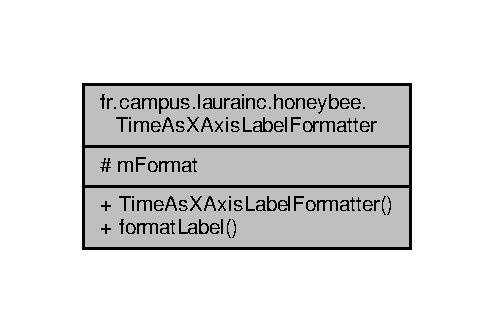
\includegraphics[width=237pt]{classfr_1_1campus_1_1laurainc_1_1honeybee_1_1_time_as_x_axis_label_formatter__coll__graph}
\end{center}
\end{figure}
\subsubsection*{Fonctions membres publiques}
\begin{DoxyCompactItemize}
\item 
\hyperlink{classfr_1_1campus_1_1laurainc_1_1honeybee_1_1_time_as_x_axis_label_formatter_acbd836cc0a90b8328a397db78a9cb082}{Time\+As\+X\+Axis\+Label\+Formatter} (String format)
\item 
String \hyperlink{classfr_1_1campus_1_1laurainc_1_1honeybee_1_1_time_as_x_axis_label_formatter_a2f5c7f8b098eb1bc82f7a47e39088820}{format\+Label} (double value, boolean is\+ValueX)
\end{DoxyCompactItemize}
\subsubsection*{Attributs protégés}
\begin{DoxyCompactItemize}
\item 
final String \hyperlink{classfr_1_1campus_1_1laurainc_1_1honeybee_1_1_time_as_x_axis_label_formatter_ab6093f1dff2db01144543e00bb1b2700}{m\+Format}
\end{DoxyCompactItemize}


\subsubsection{Documentation des constructeurs et destructeur}
\mbox{\Hypertarget{classfr_1_1campus_1_1laurainc_1_1honeybee_1_1_time_as_x_axis_label_formatter_acbd836cc0a90b8328a397db78a9cb082}\label{classfr_1_1campus_1_1laurainc_1_1honeybee_1_1_time_as_x_axis_label_formatter_acbd836cc0a90b8328a397db78a9cb082}} 
\index{fr\+::campus\+::laurainc\+::honeybee\+::\+Time\+As\+X\+Axis\+Label\+Formatter@{fr\+::campus\+::laurainc\+::honeybee\+::\+Time\+As\+X\+Axis\+Label\+Formatter}!Time\+As\+X\+Axis\+Label\+Formatter@{Time\+As\+X\+Axis\+Label\+Formatter}}
\index{Time\+As\+X\+Axis\+Label\+Formatter@{Time\+As\+X\+Axis\+Label\+Formatter}!fr\+::campus\+::laurainc\+::honeybee\+::\+Time\+As\+X\+Axis\+Label\+Formatter@{fr\+::campus\+::laurainc\+::honeybee\+::\+Time\+As\+X\+Axis\+Label\+Formatter}}
\paragraph{\texorpdfstring{Time\+As\+X\+Axis\+Label\+Formatter()}{TimeAsXAxisLabelFormatter()}}
{\footnotesize\ttfamily fr.\+campus.\+laurainc.\+honeybee.\+Time\+As\+X\+Axis\+Label\+Formatter.\+Time\+As\+X\+Axis\+Label\+Formatter (\begin{DoxyParamCaption}\item[{String}]{format }\end{DoxyParamCaption})}


\begin{DoxyCode}
00016                                                     \{
00017         \hyperlink{classfr_1_1campus_1_1laurainc_1_1honeybee_1_1_time_as_x_axis_label_formatter_ab6093f1dff2db01144543e00bb1b2700}{mFormat} = format;
00018     \}
\end{DoxyCode}


\subsubsection{Documentation des fonctions membres}
\mbox{\Hypertarget{classfr_1_1campus_1_1laurainc_1_1honeybee_1_1_time_as_x_axis_label_formatter_a2f5c7f8b098eb1bc82f7a47e39088820}\label{classfr_1_1campus_1_1laurainc_1_1honeybee_1_1_time_as_x_axis_label_formatter_a2f5c7f8b098eb1bc82f7a47e39088820}} 
\index{fr\+::campus\+::laurainc\+::honeybee\+::\+Time\+As\+X\+Axis\+Label\+Formatter@{fr\+::campus\+::laurainc\+::honeybee\+::\+Time\+As\+X\+Axis\+Label\+Formatter}!format\+Label@{format\+Label}}
\index{format\+Label@{format\+Label}!fr\+::campus\+::laurainc\+::honeybee\+::\+Time\+As\+X\+Axis\+Label\+Formatter@{fr\+::campus\+::laurainc\+::honeybee\+::\+Time\+As\+X\+Axis\+Label\+Formatter}}
\paragraph{\texorpdfstring{format\+Label()}{formatLabel()}}
{\footnotesize\ttfamily String fr.\+campus.\+laurainc.\+honeybee.\+Time\+As\+X\+Axis\+Label\+Formatter.\+format\+Label (\begin{DoxyParamCaption}\item[{double}]{value,  }\item[{boolean}]{is\+ValueX }\end{DoxyParamCaption})}


\begin{DoxyCode}
00021                                                               \{
00022         \textcolor{keywordflow}{if} (isValueX) \{
00023             Date d = \textcolor{keyword}{new} Date(0, 0, 0, (\textcolor{keywordtype}{int})value, 0);
00024             SimpleDateFormat dateFormat = \textcolor{keyword}{new} SimpleDateFormat(\hyperlink{classfr_1_1campus_1_1laurainc_1_1honeybee_1_1_time_as_x_axis_label_formatter_ab6093f1dff2db01144543e00bb1b2700}{mFormat});
00025             \textcolor{keywordflow}{return} dateFormat.format(d);
00026         \} \textcolor{keywordflow}{else} \{
00027             \textcolor{keywordflow}{return} super.formatLabel(value, isValueX);
00028         \}
00029     \}
\end{DoxyCode}


\subsubsection{Documentation des données membres}
\mbox{\Hypertarget{classfr_1_1campus_1_1laurainc_1_1honeybee_1_1_time_as_x_axis_label_formatter_ab6093f1dff2db01144543e00bb1b2700}\label{classfr_1_1campus_1_1laurainc_1_1honeybee_1_1_time_as_x_axis_label_formatter_ab6093f1dff2db01144543e00bb1b2700}} 
\index{fr\+::campus\+::laurainc\+::honeybee\+::\+Time\+As\+X\+Axis\+Label\+Formatter@{fr\+::campus\+::laurainc\+::honeybee\+::\+Time\+As\+X\+Axis\+Label\+Formatter}!m\+Format@{m\+Format}}
\index{m\+Format@{m\+Format}!fr\+::campus\+::laurainc\+::honeybee\+::\+Time\+As\+X\+Axis\+Label\+Formatter@{fr\+::campus\+::laurainc\+::honeybee\+::\+Time\+As\+X\+Axis\+Label\+Formatter}}
\paragraph{\texorpdfstring{m\+Format}{mFormat}}
{\footnotesize\ttfamily final String fr.\+campus.\+laurainc.\+honeybee.\+Time\+As\+X\+Axis\+Label\+Formatter.\+m\+Format\hspace{0.3cm}{\ttfamily [protected]}}



La documentation de cette classe a été générée à partir du fichier suivant \+:\begin{DoxyCompactItemize}
\item 
\hyperlink{_time_as_x_axis_label_formatter_8java}{Time\+As\+X\+Axis\+Label\+Formatter.\+java}\end{DoxyCompactItemize}

\section{Documentation des fichiers}
\hypertarget{alertes_8cpp}{}\subsection{Référence du fichier alertes.\+cpp}
\label{alertes_8cpp}\index{alertes.\+cpp@{alertes.\+cpp}}


Définition de la classe \hyperlink{class_alertes}{Alertes}.  


{\ttfamily \#include \char`\"{}alertes.\+h\char`\"{}}\newline
{\ttfamily \#include \char`\"{}infos\+Humidite.\+h\char`\"{}}\newline
{\ttfamily \#include \char`\"{}infos\+Pression\+Atmospherique.\+h\char`\"{}}\newline
{\ttfamily \#include \char`\"{}infos\+Temperature.\+h\char`\"{}}\newline
{\ttfamily \#include \char`\"{}infos\+Ensoleillement.\+h\char`\"{}}\newline
{\ttfamily \#include \char`\"{}infos\+Poids.\+h\char`\"{}}\newline
{\ttfamily \#include \char`\"{}infos\+Batterie.\+h\char`\"{}}\newline
{\ttfamily \#include \char`\"{}parametres.\+h\char`\"{}}\newline
{\ttfamily \#include \char`\"{}reglages\+Alertes\+Ihm.\+h\char`\"{}}\newline
{\ttfamily \#include \char`\"{}base\+De\+Donnees.\+h\char`\"{}}\newline
{\ttfamily \#include \char`\"{}simple-\/mail/\+Smtp\+Mime\char`\"{}}\newline
{\ttfamily \#include \char`\"{}ruche.\+h\char`\"{}}\newline
{\ttfamily \#include $<$Q\+Debug$>$}\newline


\subsubsection{Description détaillée}
\begin{DoxyAuthor}{Auteur}
Florentin Mellah, Enzo Rossi
\end{DoxyAuthor}
\begin{DoxyVersion}{Version}
1.\+1 
\end{DoxyVersion}

\hypertarget{alertes_8h}{}\subsection{Référence du fichier alertes.\+h}
\label{alertes_8h}\index{alertes.\+h@{alertes.\+h}}


La classe des alertes.  


{\ttfamily \#include $<$Q\+Object$>$}\newline
{\ttfamily \#include \char`\"{}parametres.\+h\char`\"{}}\newline
\subsubsection*{Classes}
\begin{DoxyCompactItemize}
\item 
class \hyperlink{class_alertes}{Alertes}
\begin{DoxyCompactList}\small\item\em La classe des alertes. \end{DoxyCompactList}\end{DoxyCompactItemize}


\subsubsection{Description détaillée}
\begin{DoxyAuthor}{Auteur}
Florentin Mellah, Enzo Rossi
\end{DoxyAuthor}
\begin{DoxyVersion}{Version}
1.\+1 
\end{DoxyVersion}

\hypertarget{alertes_activity_8java}{}\subsection{Référence du fichier alertes\+Activity.\+java}
\label{alertes_activity_8java}\index{alertes\+Activity.\+java@{alertes\+Activity.\+java}}
\subsubsection*{Classes}
\begin{DoxyCompactItemize}
\item 
class \hyperlink{classfr_1_1campus_1_1laurainc_1_1honeybee_1_1alertes_activity}{fr.\+campus.\+laurainc.\+honeybee.\+alertes\+Activity}
\end{DoxyCompactItemize}
\subsubsection*{Paquetages}
\begin{DoxyCompactItemize}
\item 
package \hyperlink{namespacefr_1_1campus_1_1laurainc_1_1honeybee}{fr.\+campus.\+laurainc.\+honeybee}
\end{DoxyCompactItemize}

\hypertarget{base_de_donnees_8cpp}{}\subsection{Référence du fichier base\+De\+Donnees.\+cpp}
\label{base_de_donnees_8cpp}\index{base\+De\+Donnees.\+cpp@{base\+De\+Donnees.\+cpp}}


Définition de la classe \hyperlink{class_base_de_donnees}{Base\+De\+Donnees}.  


{\ttfamily \#include \char`\"{}base\+De\+Donnees.\+h\char`\"{}}\newline
{\ttfamily \#include \char`\"{}parametres.\+h\char`\"{}}\newline
{\ttfamily \#include $<$Q\+Debug$>$}\newline
{\ttfamily \#include $<$Q\+Message\+Box$>$}\newline


\subsubsection{Description détaillée}
\begin{DoxyAuthor}{Auteur}
Thierry Vaira
\end{DoxyAuthor}
\begin{DoxyVersion}{Version}
0.\+2 
\end{DoxyVersion}

\hypertarget{base_de_donnees_8h}{}\subsection{Référence du fichier base\+De\+Donnees.\+h}
\label{base_de_donnees_8h}\index{base\+De\+Donnees.\+h@{base\+De\+Donnees.\+h}}


Déclaration de la classe \hyperlink{class_base_de_donnees}{Base\+De\+Donnees}.  


{\ttfamily \#include $<$Q\+Object$>$}\newline
{\ttfamily \#include $<$Qt\+Sql/\+Qt\+Sql$>$}\newline
{\ttfamily \#include $<$Q\+Sql\+Database$>$}\newline
{\ttfamily \#include $<$Q\+Mutex$>$}\newline
{\ttfamily \#include $<$Q\+String$>$}\newline
{\ttfamily \#include \char`\"{}parametres.\+h\char`\"{}}\newline
\subsubsection*{Classes}
\begin{DoxyCompactItemize}
\item 
class \hyperlink{class_base_de_donnees}{Base\+De\+Donnees}
\end{DoxyCompactItemize}


\subsubsection{Description détaillée}
\begin{DoxyAuthor}{Auteur}
Thierry V\+A\+I\+RA
\end{DoxyAuthor}
\begin{DoxyVersion}{Version}
0.\+2 
\end{DoxyVersion}

\hypertarget{_base_de_donnees_8java}{}\subsection{Référence du fichier Base\+De\+Donnees.\+java}
\label{_base_de_donnees_8java}\index{Base\+De\+Donnees.\+java@{Base\+De\+Donnees.\+java}}
\subsubsection*{Classes}
\begin{DoxyCompactItemize}
\item 
class \hyperlink{classfr_1_1campus_1_1laurainc_1_1honeybee_1_1_base_de_donnees}{fr.\+campus.\+laurainc.\+honeybee.\+Base\+De\+Donnees}
\begin{DoxyCompactList}\small\item\em Gestion d\textquotesingle{}une base de données My\+S\+QL (Singleton) \end{DoxyCompactList}\item 
class \hyperlink{classfr_1_1campus_1_1laurainc_1_1honeybee_1_1_base_de_donnees_1_1_connexion_my_sql}{fr.\+campus.\+laurainc.\+honeybee.\+Base\+De\+Donnees.\+Connexion\+My\+Sql}
\begin{DoxyCompactList}\small\item\em Classe permettant de se connecter à My\+S\+QL en arrière-\/plan. \end{DoxyCompactList}\end{DoxyCompactItemize}
\subsubsection*{Paquetages}
\begin{DoxyCompactItemize}
\item 
package \hyperlink{namespacefr_1_1campus_1_1laurainc_1_1honeybee}{fr.\+campus.\+laurainc.\+honeybee}
\end{DoxyCompactItemize}

\hypertarget{_carte_activity_8java}{}\subsection{Référence du fichier Carte\+Activity.\+java}
\label{_carte_activity_8java}\index{Carte\+Activity.\+java@{Carte\+Activity.\+java}}
\subsubsection*{Classes}
\begin{DoxyCompactItemize}
\item 
class \hyperlink{classfr_1_1campus_1_1laurainc_1_1honeybee_1_1_carte_activity}{fr.\+campus.\+laurainc.\+honeybee.\+Carte\+Activity}
\end{DoxyCompactItemize}
\subsubsection*{Paquetages}
\begin{DoxyCompactItemize}
\item 
package \hyperlink{namespacefr_1_1campus_1_1laurainc_1_1honeybee}{fr.\+campus.\+laurainc.\+honeybee}
\end{DoxyCompactItemize}

\hypertarget{_changelog_8md}{}\subsection{Référence du fichier Changelog.\+md}
\label{_changelog_8md}\index{Changelog.\+md@{Changelog.\+md}}

\hypertarget{_client_m_q_t_t_8java}{}\subsection{Référence du fichier Client\+M\+Q\+T\+T.\+java}
\label{_client_m_q_t_t_8java}\index{Client\+M\+Q\+T\+T.\+java@{Client\+M\+Q\+T\+T.\+java}}
\subsubsection*{Classes}
\begin{DoxyCompactItemize}
\item 
class \hyperlink{classfr_1_1campus_1_1laurainc_1_1honeybee_1_1_client_m_q_t_t}{fr.\+campus.\+laurainc.\+honeybee.\+Client\+M\+Q\+TT}
\end{DoxyCompactItemize}
\subsubsection*{Paquetages}
\begin{DoxyCompactItemize}
\item 
package \hyperlink{namespacefr_1_1campus_1_1laurainc_1_1honeybee}{fr.\+campus.\+laurainc.\+honeybee}
\end{DoxyCompactItemize}

\hypertarget{communication_8cpp}{}\subsection{Référence du fichier communication.\+cpp}
\label{communication_8cpp}\index{communication.\+cpp@{communication.\+cpp}}


Définition de la classe \hyperlink{class_communication}{Communication}.  


{\ttfamily \#include \char`\"{}communication.\+h\char`\"{}}\newline
{\ttfamily \#include $<$Q\+Message\+Box$>$}\newline
{\ttfamily \#include $<$Q\+Debug$>$}\newline


\subsubsection{Description détaillée}
\begin{DoxyAuthor}{Auteur}
Florentin Mellah, Enzo Rossi
\end{DoxyAuthor}
\begin{DoxyVersion}{Version}
1.\+1 
\end{DoxyVersion}

\hypertarget{communication_8h}{}\subsection{Référence du fichier communication.\+h}
\label{communication_8h}\index{communication.\+h@{communication.\+h}}


Déclaration de la classe \hyperlink{class_communication}{Communication}.  


{\ttfamily \#include $<$Qt\+Mqtt/\+Qt\+Mqtt$>$}\newline
{\ttfamily \#include $<$Qt\+Mqtt/\+Q\+Mqtt\+Client$>$}\newline
{\ttfamily \#include \char`\"{}parametres.\+h\char`\"{}}\newline
\subsubsection*{Classes}
\begin{DoxyCompactItemize}
\item 
class \hyperlink{class_communication}{Communication}
\begin{DoxyCompactList}\small\item\em La classe \hyperlink{class_communication}{Communication}. \end{DoxyCompactList}\end{DoxyCompactItemize}


\subsubsection{Description détaillée}
\begin{DoxyAuthor}{Auteur}
Florentin Mellah, Enzo Rossi
\end{DoxyAuthor}
\begin{DoxyVersion}{Version}
1.\+1 
\end{DoxyVersion}

\hypertarget{_dashboard_activity_8java}{}\subsection{Référence du fichier Dashboard\+Activity.\+java}
\label{_dashboard_activity_8java}\index{Dashboard\+Activity.\+java@{Dashboard\+Activity.\+java}}
\subsubsection*{Classes}
\begin{DoxyCompactItemize}
\item 
class \hyperlink{classfr_1_1campus_1_1laurainc_1_1honeybee_1_1_dashboard_activity}{fr.\+campus.\+laurainc.\+honeybee.\+Dashboard\+Activity}
\end{DoxyCompactItemize}
\subsubsection*{Paquetages}
\begin{DoxyCompactItemize}
\item 
package \hyperlink{namespacefr_1_1campus_1_1laurainc_1_1honeybee}{fr.\+campus.\+laurainc.\+honeybee}
\end{DoxyCompactItemize}

\hypertarget{_details_ruche_activity_8java}{}\subsection{Référence du fichier Details\+Ruche\+Activity.\+java}
\label{_details_ruche_activity_8java}\index{Details\+Ruche\+Activity.\+java@{Details\+Ruche\+Activity.\+java}}
\subsubsection*{Classes}
\begin{DoxyCompactItemize}
\item 
class \hyperlink{classfr_1_1campus_1_1laurainc_1_1honeybee_1_1_details_ruche_activity}{fr.\+campus.\+laurainc.\+honeybee.\+Details\+Ruche\+Activity}
\end{DoxyCompactItemize}
\subsubsection*{Paquetages}
\begin{DoxyCompactItemize}
\item 
package \hyperlink{namespacefr_1_1campus_1_1laurainc_1_1honeybee}{fr.\+campus.\+laurainc.\+honeybee}
\end{DoxyCompactItemize}

\hypertarget{_example_instrumented_test_8java}{}\subsection{Référence du fichier Example\+Instrumented\+Test.\+java}
\label{_example_instrumented_test_8java}\index{Example\+Instrumented\+Test.\+java@{Example\+Instrumented\+Test.\+java}}
\subsubsection*{Classes}
\begin{DoxyCompactItemize}
\item 
class \hyperlink{classfr_1_1campus_1_1laurainc_1_1honeybee_1_1_example_instrumented_test}{fr.\+campus.\+laurainc.\+honeybee.\+Example\+Instrumented\+Test}
\end{DoxyCompactItemize}
\subsubsection*{Paquetages}
\begin{DoxyCompactItemize}
\item 
package \hyperlink{namespacefr_1_1campus_1_1laurainc_1_1honeybee}{fr.\+campus.\+laurainc.\+honeybee}
\end{DoxyCompactItemize}

\hypertarget{_example_unit_test_8java}{}\subsection{Référence du fichier Example\+Unit\+Test.\+java}
\label{_example_unit_test_8java}\index{Example\+Unit\+Test.\+java@{Example\+Unit\+Test.\+java}}
\subsubsection*{Classes}
\begin{DoxyCompactItemize}
\item 
class \hyperlink{classfr_1_1campus_1_1laurainc_1_1honeybee_1_1_example_unit_test}{fr.\+campus.\+laurainc.\+honeybee.\+Example\+Unit\+Test}
\end{DoxyCompactItemize}
\subsubsection*{Paquetages}
\begin{DoxyCompactItemize}
\item 
package \hyperlink{namespacefr_1_1campus_1_1laurainc_1_1honeybee}{fr.\+campus.\+laurainc.\+honeybee}
\end{DoxyCompactItemize}

\hypertarget{_graph_activity_8java}{}\subsection{Référence du fichier Graph\+Activity.\+java}
\label{_graph_activity_8java}\index{Graph\+Activity.\+java@{Graph\+Activity.\+java}}
\subsubsection*{Classes}
\begin{DoxyCompactItemize}
\item 
class \hyperlink{classfr_1_1campus_1_1laurainc_1_1honeybee_1_1_graph_activity}{fr.\+campus.\+laurainc.\+honeybee.\+Graph\+Activity}
\end{DoxyCompactItemize}
\subsubsection*{Paquetages}
\begin{DoxyCompactItemize}
\item 
package \hyperlink{namespacefr_1_1campus_1_1laurainc_1_1honeybee}{fr.\+campus.\+laurainc.\+honeybee}
\end{DoxyCompactItemize}

\hypertarget{home_activity_8java}{}\subsection{Référence du fichier home\+Activity.\+java}
\label{home_activity_8java}\index{home\+Activity.\+java@{home\+Activity.\+java}}
\subsubsection*{Classes}
\begin{DoxyCompactItemize}
\item 
class \hyperlink{classfr_1_1campus_1_1laurainc_1_1honeybee_1_1home_activity}{fr.\+campus.\+laurainc.\+honeybee.\+home\+Activity}
\end{DoxyCompactItemize}
\subsubsection*{Paquetages}
\begin{DoxyCompactItemize}
\item 
package \hyperlink{namespacefr_1_1campus_1_1laurainc_1_1honeybee}{fr.\+campus.\+laurainc.\+honeybee}
\end{DoxyCompactItemize}

\hypertarget{_honey_bee_8java}{}\subsection{Référence du fichier Honey\+Bee.\+java}
\label{_honey_bee_8java}\index{Honey\+Bee.\+java@{Honey\+Bee.\+java}}
\subsubsection*{Classes}
\begin{DoxyCompactItemize}
\item 
class \hyperlink{classfr_1_1campus_1_1laurainc_1_1honeybee_1_1_honey_bee}{fr.\+campus.\+laurainc.\+honeybee.\+Honey\+Bee}
\begin{DoxyCompactList}\small\item\em Paramètres globaux de l\textquotesingle{}application. \end{DoxyCompactList}\end{DoxyCompactItemize}
\subsubsection*{Paquetages}
\begin{DoxyCompactItemize}
\item 
package \hyperlink{namespacefr_1_1campus_1_1laurainc_1_1honeybee}{fr.\+campus.\+laurainc.\+honeybee}
\end{DoxyCompactItemize}

\hypertarget{infos_batterie_8cpp}{}\subsection{Référence du fichier infos\+Batterie.\+cpp}
\label{infos_batterie_8cpp}\index{infos\+Batterie.\+cpp@{infos\+Batterie.\+cpp}}


Définition de la classe \hyperlink{class_infos_batterie}{Infos\+Batterie}.  


{\ttfamily \#include \char`\"{}infos\+Batterie.\+h\char`\"{}}\newline
{\ttfamily \#include $<$Q\+Debug$>$}\newline


\subsubsection{Description détaillée}
\begin{DoxyAuthor}{Auteur}
Florentin Mellah, Enzo Rossi
\end{DoxyAuthor}
\begin{DoxyVersion}{Version}
1.\+1 
\end{DoxyVersion}

\hypertarget{infos_batterie_8h}{}\subsection{Référence du fichier infos\+Batterie.\+h}
\label{infos_batterie_8h}\index{infos\+Batterie.\+h@{infos\+Batterie.\+h}}


Déclaration de la classe \hyperlink{class_infos_batterie}{Infos\+Batterie}.  


{\ttfamily \#include $<$Q\+String$>$}\newline
{\ttfamily \#include $<$Qt\+Core/\+Q\+Object$>$}\newline
\subsubsection*{Classes}
\begin{DoxyCompactItemize}
\item 
class \hyperlink{class_infos_batterie}{Infos\+Batterie}
\begin{DoxyCompactList}\small\item\em Déclaration de la classe \hyperlink{class_infos_batterie}{Infos\+Batterie}. \end{DoxyCompactList}\end{DoxyCompactItemize}


\subsubsection{Description détaillée}
\begin{DoxyAuthor}{Auteur}
Florentin Mellah, Enzo Rossi
\end{DoxyAuthor}
\begin{DoxyVersion}{Version}
1.\+1 
\end{DoxyVersion}

\hypertarget{infos_ensoleillement_8cpp}{}\subsection{Référence du fichier infos\+Ensoleillement.\+cpp}
\label{infos_ensoleillement_8cpp}\index{infos\+Ensoleillement.\+cpp@{infos\+Ensoleillement.\+cpp}}


Définition de la classe \hyperlink{class_infos_ensoleillement}{Infos\+Ensoleillement}.  


{\ttfamily \#include \char`\"{}infos\+Ensoleillement.\+h\char`\"{}}\newline
{\ttfamily \#include $<$Q\+Time$>$}\newline
{\ttfamily \#include $<$Q\+Debug$>$}\newline


\subsubsection{Description détaillée}
\begin{DoxyAuthor}{Auteur}
Florentin Mellah, Enzo Rossi
\end{DoxyAuthor}
\begin{DoxyVersion}{Version}
1.\+1 
\end{DoxyVersion}

\hypertarget{infos_ensoleillement_8h}{}\subsection{Référence du fichier infos\+Ensoleillement.\+h}
\label{infos_ensoleillement_8h}\index{infos\+Ensoleillement.\+h@{infos\+Ensoleillement.\+h}}


Déclaration de la classe \hyperlink{class_infos_ensoleillement}{Infos\+Ensoleillement}.  


{\ttfamily \#include $<$Q\+String$>$}\newline
{\ttfamily \#include $<$Qt\+Core/\+Q\+Object$>$}\newline
{\ttfamily \#include $<$Q\+Vector$>$}\newline
\subsubsection*{Classes}
\begin{DoxyCompactItemize}
\item 
class \hyperlink{class_infos_ensoleillement}{Infos\+Ensoleillement}
\begin{DoxyCompactList}\small\item\em La classe \hyperlink{class_infos_ensoleillement}{Infos\+Ensoleillement}. \end{DoxyCompactList}\end{DoxyCompactItemize}


\subsubsection{Description détaillée}
\begin{DoxyAuthor}{Auteur}
Florentin Mellah, Enzo Rossi
\end{DoxyAuthor}
\begin{DoxyVersion}{Version}
1.\+1 
\end{DoxyVersion}

\hypertarget{infos_humidite_8cpp}{}\subsection{Référence du fichier infos\+Humidite.\+cpp}
\label{infos_humidite_8cpp}\index{infos\+Humidite.\+cpp@{infos\+Humidite.\+cpp}}


Définition de la classe \hyperlink{class_infos_humidite}{Infos\+Humidite}.  


{\ttfamily \#include \char`\"{}infos\+Humidite.\+h\char`\"{}}\newline
{\ttfamily \#include $<$Q\+Time$>$}\newline
{\ttfamily \#include $<$Q\+Debug$>$}\newline


\subsubsection{Description détaillée}
\begin{DoxyAuthor}{Auteur}
Florentin Mellah, Enzo Rossi
\end{DoxyAuthor}
\begin{DoxyVersion}{Version}
1.\+1 
\end{DoxyVersion}

\hypertarget{infos_humidite_8h}{}\subsection{Référence du fichier infos\+Humidite.\+h}
\label{infos_humidite_8h}\index{infos\+Humidite.\+h@{infos\+Humidite.\+h}}


Déclaration de la classe \hyperlink{class_infos_humidite}{Infos\+Humidite}.  


{\ttfamily \#include $<$Q\+String$>$}\newline
{\ttfamily \#include $<$Qt\+Core/\+Q\+Object$>$}\newline
{\ttfamily \#include $<$Q\+Vector$>$}\newline
\subsubsection*{Classes}
\begin{DoxyCompactItemize}
\item 
class \hyperlink{class_infos_humidite}{Infos\+Humidite}
\begin{DoxyCompactList}\small\item\em La classe \hyperlink{class_infos_humidite}{Infos\+Humidite}. \end{DoxyCompactList}\end{DoxyCompactItemize}


\subsubsection{Description détaillée}
\begin{DoxyAuthor}{Auteur}
Florentin Mellah, Enzo Rossi
\end{DoxyAuthor}
\begin{DoxyVersion}{Version}
1.\+1 
\end{DoxyVersion}

\hypertarget{infos_poids_8cpp}{}\subsection{Référence du fichier infos\+Poids.\+cpp}
\label{infos_poids_8cpp}\index{infos\+Poids.\+cpp@{infos\+Poids.\+cpp}}


Défénition de la classe \hyperlink{class_infos_poids}{Infos\+Poids}.  


{\ttfamily \#include \char`\"{}infos\+Poids.\+h\char`\"{}}\newline
{\ttfamily \#include $<$Q\+Debug$>$}\newline


\subsubsection{Description détaillée}
\begin{DoxyAuthor}{Auteur}
Florentin Mellah, Enzo Rossi
\end{DoxyAuthor}
\begin{DoxyVersion}{Version}
1.\+1 
\end{DoxyVersion}

\hypertarget{infos_poids_8h}{}\subsection{Référence du fichier infos\+Poids.\+h}
\label{infos_poids_8h}\index{infos\+Poids.\+h@{infos\+Poids.\+h}}


Déclaration de la classe \hyperlink{class_infos_poids}{Infos\+Poids}.  


{\ttfamily \#include $<$Q\+String$>$}\newline
{\ttfamily \#include $<$Qt\+Core/\+Q\+Object$>$}\newline
\subsubsection*{Classes}
\begin{DoxyCompactItemize}
\item 
class \hyperlink{class_infos_poids}{Infos\+Poids}
\begin{DoxyCompactList}\small\item\em Déclaration de la classe \hyperlink{class_infos_poids}{Infos\+Poids}. \end{DoxyCompactList}\end{DoxyCompactItemize}


\subsubsection{Description détaillée}
\begin{DoxyAuthor}{Auteur}
Florentin Mellah, Enzo Rossi
\end{DoxyAuthor}
\begin{DoxyVersion}{Version}
1.\+1 
\end{DoxyVersion}

\hypertarget{infos_pression_atmospherique_8cpp}{}\subsection{Référence du fichier infos\+Pression\+Atmospherique.\+cpp}
\label{infos_pression_atmospherique_8cpp}\index{infos\+Pression\+Atmospherique.\+cpp@{infos\+Pression\+Atmospherique.\+cpp}}


Définition de la classe \hyperlink{class_infos_pression_atmospherique}{Infos\+Pression\+Atmospherique}.  


{\ttfamily \#include \char`\"{}infos\+Pression\+Atmospherique.\+h\char`\"{}}\newline
{\ttfamily \#include $<$Q\+Debug$>$}\newline
{\ttfamily \#include $<$Q\+Time$>$}\newline


\subsubsection{Description détaillée}
\begin{DoxyAuthor}{Auteur}
Florentin Mellah, Enzo Rossi
\end{DoxyAuthor}
\begin{DoxyVersion}{Version}
1.\+1 
\end{DoxyVersion}

\hypertarget{infos_pression_atmospherique_8h}{}\subsection{Référence du fichier infos\+Pression\+Atmospherique.\+h}
\label{infos_pression_atmospherique_8h}\index{infos\+Pression\+Atmospherique.\+h@{infos\+Pression\+Atmospherique.\+h}}


Déclaration de la classe \hyperlink{class_infos_pression_atmospherique}{Infos\+Pression\+Atmospherique}.  


{\ttfamily \#include $<$Q\+String$>$}\newline
{\ttfamily \#include $<$Qt\+Core/\+Q\+Object$>$}\newline
{\ttfamily \#include $<$Q\+Vector$>$}\newline
\subsubsection*{Classes}
\begin{DoxyCompactItemize}
\item 
class \hyperlink{class_infos_pression_atmospherique}{Infos\+Pression\+Atmospherique}
\begin{DoxyCompactList}\small\item\em La classe \hyperlink{class_infos_pression_atmospherique}{Infos\+Pression\+Atmospherique}. \end{DoxyCompactList}\end{DoxyCompactItemize}


\subsubsection{Description détaillée}
\begin{DoxyAuthor}{Auteur}
Florentin Mellah, Enzo Rossi
\end{DoxyAuthor}
\begin{DoxyVersion}{Version}
1.\+1 
\end{DoxyVersion}

\hypertarget{infos_temperature_8cpp}{}\subsection{Référence du fichier infos\+Temperature.\+cpp}
\label{infos_temperature_8cpp}\index{infos\+Temperature.\+cpp@{infos\+Temperature.\+cpp}}


Définition de la classe \hyperlink{class_infos_temperature}{Infos\+Temperature}.  


{\ttfamily \#include \char`\"{}infos\+Temperature.\+h\char`\"{}}\newline
{\ttfamily \#include $<$Q\+Debug$>$}\newline
{\ttfamily \#include $<$Q\+Time$>$}\newline


\subsubsection{Description détaillée}
\begin{DoxyAuthor}{Auteur}
Florentin Mellah, Enzo Rossi
\end{DoxyAuthor}
\begin{DoxyVersion}{Version}
1.\+1 
\end{DoxyVersion}

\hypertarget{infos_temperature_8h}{}\subsection{Référence du fichier infos\+Temperature.\+h}
\label{infos_temperature_8h}\index{infos\+Temperature.\+h@{infos\+Temperature.\+h}}


Déclaration de la classe \hyperlink{class_infos_temperature}{Infos\+Temperature}.  


{\ttfamily \#include $<$Q\+String$>$}\newline
{\ttfamily \#include $<$Qt\+Core/\+Q\+Object$>$}\newline
{\ttfamily \#include $<$Q\+Vector$>$}\newline
\subsubsection*{Classes}
\begin{DoxyCompactItemize}
\item 
class \hyperlink{class_infos_temperature}{Infos\+Temperature}
\begin{DoxyCompactList}\small\item\em La classe \hyperlink{class_infos_temperature}{Infos\+Temperature}. \end{DoxyCompactList}\end{DoxyCompactItemize}


\subsubsection{Description détaillée}
\begin{DoxyAuthor}{Auteur}
Florentin Mellah, Enzo Rossi
\end{DoxyAuthor}
\begin{DoxyVersion}{Version}
1.\+1 
\end{DoxyVersion}

\hypertarget{_i_n_s_t_a_l_l_8md}{}\subsection{Référence du fichier I\+N\+S\+T\+A\+L\+L.\+md}
\label{_i_n_s_t_a_l_l_8md}\index{I\+N\+S\+T\+A\+L\+L.\+md@{I\+N\+S\+T\+A\+L\+L.\+md}}

\hypertarget{main_8cpp}{}\subsection{Référence du fichier main.\+cpp}
\label{main_8cpp}\index{main.\+cpp@{main.\+cpp}}


Programme principal.  


{\ttfamily \#include \char`\"{}ruche\+Ihm.\+h\char`\"{}}\newline
{\ttfamily \#include $<$Q\+Application$>$}\newline
{\ttfamily \#include $<$Q\+String$>$}\newline
{\ttfamily \#include $<$Q\+Translator$>$}\newline
{\ttfamily \#include $<$Q\+Locale$>$}\newline
{\ttfamily \#include $<$Q\+Library\+Info$>$}\newline
{\ttfamily \#include $<$base\+De\+Donnees.\+h$>$}\newline
\subsubsection*{Fonctions}
\begin{DoxyCompactItemize}
\item 
int \hyperlink{main_8cpp_ae0665038b72011f5c680c660fcb59459}{main} (int argc, char $\ast$argv\mbox{[}$\,$\mbox{]})
\end{DoxyCompactItemize}


\subsubsection{Description détaillée}
Crée et affiche la fenêtre principale de l\textquotesingle{}application

\begin{DoxyAuthor}{Auteur}
Florentin Mellah, Enzo Rossi
\end{DoxyAuthor}
\begin{DoxyVersion}{Version}
1.\+1 
\end{DoxyVersion}


\subsubsection{Documentation des fonctions}
\mbox{\Hypertarget{main_8cpp_ae0665038b72011f5c680c660fcb59459}\label{main_8cpp_ae0665038b72011f5c680c660fcb59459}} 
\index{main.\+cpp@{main.\+cpp}!main@{main}}
\index{main@{main}!main.\+cpp@{main.\+cpp}}
\paragraph{\texorpdfstring{main()}{main()}}
{\footnotesize\ttfamily main (\begin{DoxyParamCaption}\item[{int}]{argc,  }\item[{char $\ast$}]{argv\mbox{[}$\,$\mbox{]} }\end{DoxyParamCaption})}


\begin{DoxyParams}{Paramètres}
{\em argc} & \\
\hline
{\em argv\mbox{[}$\,$\mbox{]}} & \\
\hline
\end{DoxyParams}
\begin{DoxyReturn}{Renvoie}
int 
\end{DoxyReturn}

\begin{DoxyCode}
00029 \{
00030     QApplication a(argc, argv);
00031     QString locale = QLocale::system().name().section(\textcolor{charliteral}{'\_'}, 0, 0);
00032     QTranslator translator;
00033     translator.load(QString(\textcolor{stringliteral}{"qt\_"}) + locale, QLibraryInfo::location(QLibraryInfo::TranslationsPath));
00034     a.installTranslator(&translator);
00035 
00036     \hyperlink{class_ruche_ihm}{RucheIhm} w;
00037     w.show();
00038 
00039     \textcolor{keywordflow}{return} a.exec();
00040 \}
\end{DoxyCode}

\hypertarget{_main_activity_8java}{}\subsection{Référence du fichier Main\+Activity.\+java}
\label{_main_activity_8java}\index{Main\+Activity.\+java@{Main\+Activity.\+java}}
\subsubsection*{Classes}
\begin{DoxyCompactItemize}
\item 
class \hyperlink{classfr_1_1campus_1_1laurainc_1_1honeybee_1_1_main_activity}{fr.\+campus.\+laurainc.\+honeybee.\+Main\+Activity}
\begin{DoxyCompactList}\small\item\em Activité principale de l\textquotesingle{}application (Thread UI) \end{DoxyCompactList}\end{DoxyCompactItemize}
\subsubsection*{Paquetages}
\begin{DoxyCompactItemize}
\item 
package \hyperlink{namespacefr_1_1campus_1_1laurainc_1_1honeybee}{fr.\+campus.\+laurainc.\+honeybee}
\end{DoxyCompactItemize}

\hypertarget{_nouvelle_ruche_activity_8java}{}\subsection{Référence du fichier Nouvelle\+Ruche\+Activity.\+java}
\label{_nouvelle_ruche_activity_8java}\index{Nouvelle\+Ruche\+Activity.\+java@{Nouvelle\+Ruche\+Activity.\+java}}
\subsubsection*{Classes}
\begin{DoxyCompactItemize}
\item 
class \hyperlink{classfr_1_1campus_1_1laurainc_1_1honeybee_1_1_nouvelle_ruche_activity}{fr.\+campus.\+laurainc.\+honeybee.\+Nouvelle\+Ruche\+Activity}
\end{DoxyCompactItemize}
\subsubsection*{Paquetages}
\begin{DoxyCompactItemize}
\item 
package \hyperlink{namespacefr_1_1campus_1_1laurainc_1_1honeybee}{fr.\+campus.\+laurainc.\+honeybee}
\end{DoxyCompactItemize}

\hypertarget{nouvelle_ruche_ihm_8cpp}{}\subsection{Référence du fichier nouvelle\+Ruche\+Ihm.\+cpp}
\label{nouvelle_ruche_ihm_8cpp}\index{nouvelle\+Ruche\+Ihm.\+cpp@{nouvelle\+Ruche\+Ihm.\+cpp}}


La classe \hyperlink{class_nouvelle_ruche_ihm}{Nouvelle\+Ruche\+Ihm}.  


{\ttfamily \#include \char`\"{}nouvelle\+Ruche\+Ihm.\+h\char`\"{}}\newline
{\ttfamily \#include \char`\"{}ui\+\_\+nouvelle\+Ruche\+Ihm.\+h\char`\"{}}\newline
{\ttfamily \#include \char`\"{}base\+De\+Donnees.\+h\char`\"{}}\newline
{\ttfamily \#include $<$Q\+Message\+Box$>$}\newline


\subsubsection{Description détaillée}
Définition de la classe \hyperlink{class_ruche_ihm}{Ruche\+Ihm}.

\begin{DoxyAuthor}{Auteur}
Florentin Mellah, Enzo Rossi
\end{DoxyAuthor}
\begin{DoxyVersion}{Version}
1.\+1 
\end{DoxyVersion}

\hypertarget{nouvelle_ruche_ihm_8h}{}\subsection{Référence du fichier nouvelle\+Ruche\+Ihm.\+h}
\label{nouvelle_ruche_ihm_8h}\index{nouvelle\+Ruche\+Ihm.\+h@{nouvelle\+Ruche\+Ihm.\+h}}
{\ttfamily \#include $<$Q\+Dialog$>$}\newline
\subsubsection*{Classes}
\begin{DoxyCompactItemize}
\item 
class \hyperlink{class_nouvelle_ruche_ihm}{Nouvelle\+Ruche\+Ihm}
\begin{DoxyCompactList}\small\item\em Déclaration de la classe \hyperlink{class_nouvelle_ruche_ihm}{Nouvelle\+Ruche\+Ihm}. \end{DoxyCompactList}\end{DoxyCompactItemize}
\subsubsection*{Espaces de nommage}
\begin{DoxyCompactItemize}
\item 
 \hyperlink{namespace_ui}{Ui}
\end{DoxyCompactItemize}

\hypertarget{parametres_8h}{}\subsection{Référence du fichier parametres.\+h}
\label{parametres_8h}\index{parametres.\+h@{parametres.\+h}}


Paramètres généraux de l\textquotesingle{}application.  


\subsubsection*{Macros}
\begin{DoxyCompactItemize}
\item 
\#define \hyperlink{parametres_8h_ace364d1ce44aa9f79bcff6e3752c4a5f}{A\+P\+P\+\_\+\+T\+I\+T\+RE}~\char`\"{}Projet \hyperlink{class_ruche}{Ruche} 2019\char`\"{}
\item 
\#define \hyperlink{parametres_8h_a423559dc987673b8aacaa9f369839bb0}{B\+D\+D\+\_\+\+S\+E\+R\+V\+E\+UR}~\char`\"{}192.\+168.\+52.\+119\char`\"{}
\item 
\#define \hyperlink{parametres_8h_a88b5f5b81fa534553c68802384beff2c}{B\+D\+D\+\_\+\+U\+S\+E\+R\+N\+A\+ME}~\char`\"{}fmellah\char`\"{}
\item 
\#define \hyperlink{parametres_8h_ae2ded9166ed2553182545e97514c04f7}{B\+D\+D\+\_\+\+P\+A\+S\+S\+W\+O\+RD}~\char`\"{}password\char`\"{}
\item 
\#define \hyperlink{parametres_8h_a45f8f15b8f9a7ab4c2b219038ff64f6b}{B\+D\+D\+\_\+\+N\+O\+M\+B\+A\+SE}~\char`\"{}ruches\char`\"{}
\item 
\#define \hyperlink{parametres_8h_a7ef65c771828d75412034ca6380f66c4}{T\+T\+N\+\_\+\+S\+E\+R\+V\+E\+UR}~\char`\"{}eu.\+thethings.\+network\char`\"{}
\item 
\#define \hyperlink{parametres_8h_abea0c88db594f8dc7bc483aaa71eedf4}{T\+T\+N\+\_\+\+P\+O\+RT}~1883
\item 
\#define \hyperlink{parametres_8h_af539766e9c089423c25dd4b7005b1563}{T\+T\+N\+\_\+\+U\+S\+E\+R\+N\+A\+ME}~\char`\"{}mes\+\_\+ruches\char`\"{}
\item 
\#define \hyperlink{parametres_8h_a63e412d47c6b5d8189bcc70c32ace402}{T\+T\+N\+\_\+\+P\+A\+S\+S\+W\+O\+RD}~\char`\"{}ttn-\/account-\/v2.\+vC-\/aq\+M\+Rn\+L\+Lz\+Gk\+Nj\+O\+D\+Wgy81k\+Lqzx\+B\+P\+A\+T8\+\_\+mE-\/L7\+U2\+C\+\_\+w\char`\"{}
\item 
\#define \hyperlink{parametres_8h_a40e679ee59c74bda430a6c7498d7c21e}{T\+T\+N\+\_\+\+T\+O\+P\+IC}~\char`\"{}mes\+\_\+ruches/devices/ruche\+\_\+1/up\char`\"{}
\item 
\#define \hyperlink{parametres_8h_a45133c820662f13b719dcc1729242e61}{T\+T\+N\+\_\+\+E\+M\+A\+IL}~\char`\"{}florentinmellah@gmail.\+com\char`\"{}
\item 
\#define \hyperlink{parametres_8h_a4a0b02d56c77af5d5aceb6c9f57cfb31}{U\+S\+E\+R\+\_\+\+G\+M\+A\+IL}~Q\+Latin1\+String(\char`\"{}bee.\+honey.\+bts@gmail.\+com\char`\"{})
\item 
\#define \hyperlink{parametres_8h_a29c7597b5c4dfd015628a777f545bcb2}{P\+A\+S\+S\+W\+O\+R\+D\+\_\+\+G\+M\+A\+IL}~Q\+Latin1\+String(\char`\"{}ruches123\char`\"{})
\item 
\#define \hyperlink{parametres_8h_a76f490066655530a774202e6204f2a92}{T\+E\+M\+P\+E\+R\+A\+T\+U\+R\+E\+\_\+\+I\+N\+T\+E\+R\+I\+E\+U\+R\+\_\+\+S\+E\+U\+I\+L\+\_\+\+M\+AX}~35.\+0
\item 
\#define \hyperlink{parametres_8h_a1f78dd3105c514060033c23f7b40a899}{T\+E\+M\+P\+E\+R\+A\+T\+U\+R\+E\+\_\+\+I\+N\+T\+E\+R\+I\+E\+U\+R\+\_\+\+S\+E\+U\+I\+L\+\_\+\+M\+IN}~25.
\item 
\#define \hyperlink{parametres_8h_afc1996946dfec64accdaa88f4e313058}{H\+U\+M\+I\+D\+I\+T\+E\+\_\+\+I\+N\+T\+E\+R\+I\+E\+U\+R\+\_\+\+S\+E\+U\+I\+L\+\_\+\+M\+AX}~30.
\item 
\#define \hyperlink{parametres_8h_a123e6e1d82333f6e038d37ef506d5762}{H\+U\+M\+I\+D\+I\+T\+E\+\_\+\+I\+N\+T\+E\+R\+I\+E\+U\+R\+\_\+\+S\+E\+U\+I\+L\+\_\+\+M\+IN}~20.
\item 
\#define \hyperlink{parametres_8h_a7630cd07e0f037b4057157febd9644fd}{T\+E\+M\+P\+E\+R\+A\+T\+U\+R\+E\+\_\+\+E\+X\+T\+E\+R\+I\+E\+U\+R\+\_\+\+S\+E\+U\+I\+L\+\_\+\+M\+AX}~35.
\item 
\#define \hyperlink{parametres_8h_aeb90c8fd31e6aa6473edd143ce70e137}{T\+E\+M\+P\+E\+R\+A\+T\+U\+R\+E\+\_\+\+E\+X\+T\+E\+R\+I\+E\+U\+R\+\_\+\+S\+E\+U\+I\+L\+\_\+\+M\+IN}~5.
\item 
\#define \hyperlink{parametres_8h_a25f8411ff3fd72788fdcd7487e7e8d28}{H\+U\+M\+I\+D\+I\+T\+E\+\_\+\+E\+X\+T\+E\+R\+I\+E\+U\+R\+\_\+\+S\+E\+U\+I\+L\+\_\+\+M\+AX}~35.
\item 
\#define \hyperlink{parametres_8h_afc00f65688c19bd56711c244827c2c27}{H\+U\+M\+I\+D\+I\+T\+E\+\_\+\+E\+X\+T\+E\+R\+I\+E\+U\+R\+\_\+\+S\+E\+U\+I\+L\+\_\+\+M\+IN}~20.
\item 
\#define \hyperlink{parametres_8h_a70a55fd4037201bf606fc9e9d54e61cb}{P\+R\+E\+S\+S\+I\+O\+N\+\_\+\+A\+T\+M\+O\+S\+P\+H\+E\+R\+I\+Q\+U\+E\+\_\+\+S\+E\+U\+I\+L\+\_\+\+M\+IN}~1000.
\item 
\#define \hyperlink{parametres_8h_a2d439ba3af9708601a7ae0edf3584d98}{P\+R\+E\+S\+S\+I\+O\+N\+\_\+\+A\+T\+M\+O\+S\+P\+H\+E\+R\+I\+Q\+U\+E\+\_\+\+S\+E\+U\+I\+L\+\_\+\+M\+AX}~1200.
\item 
\#define \hyperlink{parametres_8h_a41d2727214068bc11cea2e021fb6b237}{P\+O\+I\+D\+S\+\_\+\+S\+E\+U\+I\+L\+\_\+\+M\+AX}~100.
\item 
\#define \hyperlink{parametres_8h_a289e59d08fbd111c6a5bd8a526a8098b}{P\+O\+I\+D\+S\+\_\+\+S\+E\+U\+I\+L\+\_\+\+M\+IN}~35.
\item 
\#define \hyperlink{parametres_8h_a095aa84e44055a2fa68760735cb847df}{E\+N\+S\+O\+L\+E\+I\+L\+L\+E\+M\+E\+N\+T\+\_\+\+S\+E\+U\+I\+L\+\_\+\+M\+AX}~1000.
\item 
\#define \hyperlink{parametres_8h_a1174d9c2d3ff7e8a5e464d7e0a20e1a9}{E\+N\+S\+O\+L\+E\+I\+L\+L\+E\+M\+E\+N\+T\+\_\+\+S\+E\+U\+I\+L\+\_\+\+M\+IN}~10.
\item 
\#define \hyperlink{parametres_8h_a56d8e839e7d59a28e76829be161a0530}{B\+A\+T\+T\+E\+R\+I\+E\+\_\+\+S\+E\+U\+I\+L\+\_\+\+M\+IN}~25.
\end{DoxyCompactItemize}
\subsubsection*{Énumérations}
\begin{DoxyCompactItemize}
\item 
enum \hyperlink{parametres_8h_aaa6de8207c94675264c90b10b613368d}{Seuils\+Alertes} \{ \hyperlink{parametres_8h_aaa6de8207c94675264c90b10b613368dabc650d9700ae19f2696e6a6e3f9ab067}{trop\+Haut} = 0, 
\hyperlink{parametres_8h_aaa6de8207c94675264c90b10b613368da4257e2f8921856770c8266f55c937295}{trop\+Bas} = 1, 
\hyperlink{parametres_8h_aaa6de8207c94675264c90b10b613368da5ac8ec3b54d90a07c6bb5a77ef971821}{bon} = 2
 \}
\item 
enum \hyperlink{parametres_8h_a83a725fd153179a2bd97afcc8307737b}{Type\+Alertes} \{ \newline
\hyperlink{parametres_8h_a83a725fd153179a2bd97afcc8307737ba6d07a737b602e59b2350e913e4763724}{alerte\+Temperature\+Interieur} = 0, 
\hyperlink{parametres_8h_a83a725fd153179a2bd97afcc8307737ba300b33d38ff264e971908d263fbfd1bb}{alerte\+Temperature\+Exterieur} = 1, 
\hyperlink{parametres_8h_a83a725fd153179a2bd97afcc8307737bac0e80b2d9b7f04033abc44ebcf61883a}{alerte\+Humidite\+Interieur} = 2, 
\hyperlink{parametres_8h_a83a725fd153179a2bd97afcc8307737bacda66fabe33c8c197f8ff098a952fca3}{alerte\+Humidite\+Exterieur} = 3, 
\newline
\hyperlink{parametres_8h_a83a725fd153179a2bd97afcc8307737ba3b3b9fe16ae965531aca47449d865ce1}{alerte\+Pression\+Atmospherique} = 4, 
\hyperlink{parametres_8h_a83a725fd153179a2bd97afcc8307737ba130a82230092934eb515b95603d12956}{alerte\+Poids} = 5, 
\hyperlink{parametres_8h_a83a725fd153179a2bd97afcc8307737ba256a82c8886c1902dc7a078868434f83}{alerte\+Ensoleillement} = 6, 
\hyperlink{parametres_8h_a83a725fd153179a2bd97afcc8307737ba11c71364df2afd149875ebfe0238ef7e}{alerte\+Batterie} = 7, 
\newline
\hyperlink{parametres_8h_a83a725fd153179a2bd97afcc8307737ba673fe6d70f1b196ef95a63009d855e08}{toutes\+Les\+Alertes} = 8
 \}
\item 
enum \hyperlink{parametres_8h_a0fe68caa1e9147addc96657cc822b937}{Ports\+T\+TN} \{ \newline
\hyperlink{parametres_8h_a0fe68caa1e9147addc96657cc822b937aaabf64e5057c44a19cf8f4ea1f0fa5b5}{port\+Inconnu} = 0, 
\hyperlink{parametres_8h_a0fe68caa1e9147addc96657cc822b937acbcf2a22f624d13088717cf70c7d8bae}{port\+Mesure\+Energie} = 1, 
\hyperlink{parametres_8h_a0fe68caa1e9147addc96657cc822b937a8f92167c600b17ed99cfc3f3f67a537a}{port\+Mesure\+Poids}, 
\hyperlink{parametres_8h_a0fe68caa1e9147addc96657cc822b937a88419e467bcdd4d9d15dea841fe45d62}{port\+Mesure\+Ruche}, 
\newline
\hyperlink{parametres_8h_a0fe68caa1e9147addc96657cc822b937a074d78639f6ae7cab707f31538144074}{port\+Mesure\+Environement}, 
\hyperlink{parametres_8h_a0fe68caa1e9147addc96657cc822b937a2e10cce7b58eecdeddb0e43eaed5a1c8}{port\+Mesure\+Ensoleillement}, 
\hyperlink{parametres_8h_a0fe68caa1e9147addc96657cc822b937a460fde8547d807206e876e2a622794fc}{port\+Vol}, 
\hyperlink{parametres_8h_a0fe68caa1e9147addc96657cc822b937a5fb860989b1bead466485e87c0a8b0d2}{nb\+Ports\+T\+TN}
 \}
\end{DoxyCompactItemize}


\subsubsection{Description détaillée}
\begin{DoxyAuthor}{Auteur}
Florentin Mellah, Enzo Rossi
\end{DoxyAuthor}
\begin{DoxyVersion}{Version}
1.\+1 
\end{DoxyVersion}


\subsubsection{Documentation des macros}
\mbox{\Hypertarget{parametres_8h_ace364d1ce44aa9f79bcff6e3752c4a5f}\label{parametres_8h_ace364d1ce44aa9f79bcff6e3752c4a5f}} 
\index{parametres.\+h@{parametres.\+h}!A\+P\+P\+\_\+\+T\+I\+T\+RE@{A\+P\+P\+\_\+\+T\+I\+T\+RE}}
\index{A\+P\+P\+\_\+\+T\+I\+T\+RE@{A\+P\+P\+\_\+\+T\+I\+T\+RE}!parametres.\+h@{parametres.\+h}}
\paragraph{\texorpdfstring{A\+P\+P\+\_\+\+T\+I\+T\+RE}{APP\_TITRE}}
{\footnotesize\ttfamily \#define A\+P\+P\+\_\+\+T\+I\+T\+RE~\char`\"{}Projet \hyperlink{class_ruche}{Ruche} 2019\char`\"{}}



Référencé par \hyperlink{class_ruche_ihm_a7f66af552d9e7ba0d00437ff3b330706}{Ruche\+Ihm\+::afficher\+Mesures\+Journalieres\+Selectionnee()}, \hyperlink{class_base_de_donnees_ac20da193923a9bfea5e38ee5a54820cd}{Base\+De\+Donnees\+::connecter()}, \hyperlink{class_communication_af71587fb1ee9b7460345b7c12372a1eb}{Communication\+::connecte\+T\+T\+N()}, \hyperlink{class_ruche_ihm_ab8db02641e73f348fd6162321a3765da}{Ruche\+Ihm\+::ouvrir\+Reglages\+Alertes()}, \hyperlink{class_nouvelle_ruche_ihm_a268e781b033f2531ca5eab19cc828fdc}{Nouvelle\+Ruche\+Ihm\+::recevoir\+Donnee\+Ajout\+Ruche()}, et \hyperlink{class_ruche_ihm_a85729b1ae4f3dfb5130eb45f5a426e3c}{Ruche\+Ihm\+::supprimer\+Ruche()}.

\mbox{\Hypertarget{parametres_8h_a56d8e839e7d59a28e76829be161a0530}\label{parametres_8h_a56d8e839e7d59a28e76829be161a0530}} 
\index{parametres.\+h@{parametres.\+h}!B\+A\+T\+T\+E\+R\+I\+E\+\_\+\+S\+E\+U\+I\+L\+\_\+\+M\+IN@{B\+A\+T\+T\+E\+R\+I\+E\+\_\+\+S\+E\+U\+I\+L\+\_\+\+M\+IN}}
\index{B\+A\+T\+T\+E\+R\+I\+E\+\_\+\+S\+E\+U\+I\+L\+\_\+\+M\+IN@{B\+A\+T\+T\+E\+R\+I\+E\+\_\+\+S\+E\+U\+I\+L\+\_\+\+M\+IN}!parametres.\+h@{parametres.\+h}}
\paragraph{\texorpdfstring{B\+A\+T\+T\+E\+R\+I\+E\+\_\+\+S\+E\+U\+I\+L\+\_\+\+M\+IN}{BATTERIE\_SEUIL\_MIN}}
{\footnotesize\ttfamily \#define B\+A\+T\+T\+E\+R\+I\+E\+\_\+\+S\+E\+U\+I\+L\+\_\+\+M\+IN~25.}

\mbox{\Hypertarget{parametres_8h_a45f8f15b8f9a7ab4c2b219038ff64f6b}\label{parametres_8h_a45f8f15b8f9a7ab4c2b219038ff64f6b}} 
\index{parametres.\+h@{parametres.\+h}!B\+D\+D\+\_\+\+N\+O\+M\+B\+A\+SE@{B\+D\+D\+\_\+\+N\+O\+M\+B\+A\+SE}}
\index{B\+D\+D\+\_\+\+N\+O\+M\+B\+A\+SE@{B\+D\+D\+\_\+\+N\+O\+M\+B\+A\+SE}!parametres.\+h@{parametres.\+h}}
\paragraph{\texorpdfstring{B\+D\+D\+\_\+\+N\+O\+M\+B\+A\+SE}{BDD\_NOMBASE}}
{\footnotesize\ttfamily \#define B\+D\+D\+\_\+\+N\+O\+M\+B\+A\+SE~\char`\"{}ruches\char`\"{}}



Référencé par \hyperlink{class_alertes_ad2e4e3907f97bdd06840dfeee0a87ddb}{Alertes\+::\+Alertes()}, \hyperlink{class_nouvelle_ruche_ihm_a338b9af0b96ed0839a8d5008c8c89cc4}{Nouvelle\+Ruche\+Ihm\+::\+Nouvelle\+Ruche\+Ihm()}, \hyperlink{class_reglages_alertes_ihm_ae6337f2d05a3184e48bf5022a91f06c7}{Reglages\+Alertes\+Ihm\+::\+Reglages\+Alertes\+Ihm()}, \hyperlink{class_ruche_a8b4ee3752d984c5acee93b990db7939a}{Ruche\+::\+Ruche()}, et \hyperlink{class_ruche_ihm_a04c2544ba4e9cca6c38f553c32d63dee}{Ruche\+Ihm\+::\+Ruche\+Ihm()}.

\mbox{\Hypertarget{parametres_8h_ae2ded9166ed2553182545e97514c04f7}\label{parametres_8h_ae2ded9166ed2553182545e97514c04f7}} 
\index{parametres.\+h@{parametres.\+h}!B\+D\+D\+\_\+\+P\+A\+S\+S\+W\+O\+RD@{B\+D\+D\+\_\+\+P\+A\+S\+S\+W\+O\+RD}}
\index{B\+D\+D\+\_\+\+P\+A\+S\+S\+W\+O\+RD@{B\+D\+D\+\_\+\+P\+A\+S\+S\+W\+O\+RD}!parametres.\+h@{parametres.\+h}}
\paragraph{\texorpdfstring{B\+D\+D\+\_\+\+P\+A\+S\+S\+W\+O\+RD}{BDD\_PASSWORD}}
{\footnotesize\ttfamily \#define B\+D\+D\+\_\+\+P\+A\+S\+S\+W\+O\+RD~\char`\"{}password\char`\"{}}



Référencé par \hyperlink{class_alertes_ad2e4e3907f97bdd06840dfeee0a87ddb}{Alertes\+::\+Alertes()}, \hyperlink{class_nouvelle_ruche_ihm_a338b9af0b96ed0839a8d5008c8c89cc4}{Nouvelle\+Ruche\+Ihm\+::\+Nouvelle\+Ruche\+Ihm()}, \hyperlink{class_reglages_alertes_ihm_ae6337f2d05a3184e48bf5022a91f06c7}{Reglages\+Alertes\+Ihm\+::\+Reglages\+Alertes\+Ihm()}, \hyperlink{class_ruche_a8b4ee3752d984c5acee93b990db7939a}{Ruche\+::\+Ruche()}, et \hyperlink{class_ruche_ihm_a04c2544ba4e9cca6c38f553c32d63dee}{Ruche\+Ihm\+::\+Ruche\+Ihm()}.

\mbox{\Hypertarget{parametres_8h_a423559dc987673b8aacaa9f369839bb0}\label{parametres_8h_a423559dc987673b8aacaa9f369839bb0}} 
\index{parametres.\+h@{parametres.\+h}!B\+D\+D\+\_\+\+S\+E\+R\+V\+E\+UR@{B\+D\+D\+\_\+\+S\+E\+R\+V\+E\+UR}}
\index{B\+D\+D\+\_\+\+S\+E\+R\+V\+E\+UR@{B\+D\+D\+\_\+\+S\+E\+R\+V\+E\+UR}!parametres.\+h@{parametres.\+h}}
\paragraph{\texorpdfstring{B\+D\+D\+\_\+\+S\+E\+R\+V\+E\+UR}{BDD\_SERVEUR}}
{\footnotesize\ttfamily \#define B\+D\+D\+\_\+\+S\+E\+R\+V\+E\+UR~\char`\"{}192.\+168.\+52.\+119\char`\"{}}



Référencé par \hyperlink{class_alertes_ad2e4e3907f97bdd06840dfeee0a87ddb}{Alertes\+::\+Alertes()}, \hyperlink{class_nouvelle_ruche_ihm_a338b9af0b96ed0839a8d5008c8c89cc4}{Nouvelle\+Ruche\+Ihm\+::\+Nouvelle\+Ruche\+Ihm()}, \hyperlink{class_reglages_alertes_ihm_ae6337f2d05a3184e48bf5022a91f06c7}{Reglages\+Alertes\+Ihm\+::\+Reglages\+Alertes\+Ihm()}, \hyperlink{class_ruche_a8b4ee3752d984c5acee93b990db7939a}{Ruche\+::\+Ruche()}, et \hyperlink{class_ruche_ihm_a04c2544ba4e9cca6c38f553c32d63dee}{Ruche\+Ihm\+::\+Ruche\+Ihm()}.

\mbox{\Hypertarget{parametres_8h_a88b5f5b81fa534553c68802384beff2c}\label{parametres_8h_a88b5f5b81fa534553c68802384beff2c}} 
\index{parametres.\+h@{parametres.\+h}!B\+D\+D\+\_\+\+U\+S\+E\+R\+N\+A\+ME@{B\+D\+D\+\_\+\+U\+S\+E\+R\+N\+A\+ME}}
\index{B\+D\+D\+\_\+\+U\+S\+E\+R\+N\+A\+ME@{B\+D\+D\+\_\+\+U\+S\+E\+R\+N\+A\+ME}!parametres.\+h@{parametres.\+h}}
\paragraph{\texorpdfstring{B\+D\+D\+\_\+\+U\+S\+E\+R\+N\+A\+ME}{BDD\_USERNAME}}
{\footnotesize\ttfamily \#define B\+D\+D\+\_\+\+U\+S\+E\+R\+N\+A\+ME~\char`\"{}fmellah\char`\"{}}



Référencé par \hyperlink{class_alertes_ad2e4e3907f97bdd06840dfeee0a87ddb}{Alertes\+::\+Alertes()}, \hyperlink{class_nouvelle_ruche_ihm_a338b9af0b96ed0839a8d5008c8c89cc4}{Nouvelle\+Ruche\+Ihm\+::\+Nouvelle\+Ruche\+Ihm()}, \hyperlink{class_reglages_alertes_ihm_ae6337f2d05a3184e48bf5022a91f06c7}{Reglages\+Alertes\+Ihm\+::\+Reglages\+Alertes\+Ihm()}, \hyperlink{class_ruche_a8b4ee3752d984c5acee93b990db7939a}{Ruche\+::\+Ruche()}, et \hyperlink{class_ruche_ihm_a04c2544ba4e9cca6c38f553c32d63dee}{Ruche\+Ihm\+::\+Ruche\+Ihm()}.

\mbox{\Hypertarget{parametres_8h_a095aa84e44055a2fa68760735cb847df}\label{parametres_8h_a095aa84e44055a2fa68760735cb847df}} 
\index{parametres.\+h@{parametres.\+h}!E\+N\+S\+O\+L\+E\+I\+L\+L\+E\+M\+E\+N\+T\+\_\+\+S\+E\+U\+I\+L\+\_\+\+M\+AX@{E\+N\+S\+O\+L\+E\+I\+L\+L\+E\+M\+E\+N\+T\+\_\+\+S\+E\+U\+I\+L\+\_\+\+M\+AX}}
\index{E\+N\+S\+O\+L\+E\+I\+L\+L\+E\+M\+E\+N\+T\+\_\+\+S\+E\+U\+I\+L\+\_\+\+M\+AX@{E\+N\+S\+O\+L\+E\+I\+L\+L\+E\+M\+E\+N\+T\+\_\+\+S\+E\+U\+I\+L\+\_\+\+M\+AX}!parametres.\+h@{parametres.\+h}}
\paragraph{\texorpdfstring{E\+N\+S\+O\+L\+E\+I\+L\+L\+E\+M\+E\+N\+T\+\_\+\+S\+E\+U\+I\+L\+\_\+\+M\+AX}{ENSOLEILLEMENT\_SEUIL\_MAX}}
{\footnotesize\ttfamily \#define E\+N\+S\+O\+L\+E\+I\+L\+L\+E\+M\+E\+N\+T\+\_\+\+S\+E\+U\+I\+L\+\_\+\+M\+AX~1000.}

\mbox{\Hypertarget{parametres_8h_a1174d9c2d3ff7e8a5e464d7e0a20e1a9}\label{parametres_8h_a1174d9c2d3ff7e8a5e464d7e0a20e1a9}} 
\index{parametres.\+h@{parametres.\+h}!E\+N\+S\+O\+L\+E\+I\+L\+L\+E\+M\+E\+N\+T\+\_\+\+S\+E\+U\+I\+L\+\_\+\+M\+IN@{E\+N\+S\+O\+L\+E\+I\+L\+L\+E\+M\+E\+N\+T\+\_\+\+S\+E\+U\+I\+L\+\_\+\+M\+IN}}
\index{E\+N\+S\+O\+L\+E\+I\+L\+L\+E\+M\+E\+N\+T\+\_\+\+S\+E\+U\+I\+L\+\_\+\+M\+IN@{E\+N\+S\+O\+L\+E\+I\+L\+L\+E\+M\+E\+N\+T\+\_\+\+S\+E\+U\+I\+L\+\_\+\+M\+IN}!parametres.\+h@{parametres.\+h}}
\paragraph{\texorpdfstring{E\+N\+S\+O\+L\+E\+I\+L\+L\+E\+M\+E\+N\+T\+\_\+\+S\+E\+U\+I\+L\+\_\+\+M\+IN}{ENSOLEILLEMENT\_SEUIL\_MIN}}
{\footnotesize\ttfamily \#define E\+N\+S\+O\+L\+E\+I\+L\+L\+E\+M\+E\+N\+T\+\_\+\+S\+E\+U\+I\+L\+\_\+\+M\+IN~10.}

\mbox{\Hypertarget{parametres_8h_a25f8411ff3fd72788fdcd7487e7e8d28}\label{parametres_8h_a25f8411ff3fd72788fdcd7487e7e8d28}} 
\index{parametres.\+h@{parametres.\+h}!H\+U\+M\+I\+D\+I\+T\+E\+\_\+\+E\+X\+T\+E\+R\+I\+E\+U\+R\+\_\+\+S\+E\+U\+I\+L\+\_\+\+M\+AX@{H\+U\+M\+I\+D\+I\+T\+E\+\_\+\+E\+X\+T\+E\+R\+I\+E\+U\+R\+\_\+\+S\+E\+U\+I\+L\+\_\+\+M\+AX}}
\index{H\+U\+M\+I\+D\+I\+T\+E\+\_\+\+E\+X\+T\+E\+R\+I\+E\+U\+R\+\_\+\+S\+E\+U\+I\+L\+\_\+\+M\+AX@{H\+U\+M\+I\+D\+I\+T\+E\+\_\+\+E\+X\+T\+E\+R\+I\+E\+U\+R\+\_\+\+S\+E\+U\+I\+L\+\_\+\+M\+AX}!parametres.\+h@{parametres.\+h}}
\paragraph{\texorpdfstring{H\+U\+M\+I\+D\+I\+T\+E\+\_\+\+E\+X\+T\+E\+R\+I\+E\+U\+R\+\_\+\+S\+E\+U\+I\+L\+\_\+\+M\+AX}{HUMIDITE\_EXTERIEUR\_SEUIL\_MAX}}
{\footnotesize\ttfamily \#define H\+U\+M\+I\+D\+I\+T\+E\+\_\+\+E\+X\+T\+E\+R\+I\+E\+U\+R\+\_\+\+S\+E\+U\+I\+L\+\_\+\+M\+AX~35.}

\mbox{\Hypertarget{parametres_8h_afc00f65688c19bd56711c244827c2c27}\label{parametres_8h_afc00f65688c19bd56711c244827c2c27}} 
\index{parametres.\+h@{parametres.\+h}!H\+U\+M\+I\+D\+I\+T\+E\+\_\+\+E\+X\+T\+E\+R\+I\+E\+U\+R\+\_\+\+S\+E\+U\+I\+L\+\_\+\+M\+IN@{H\+U\+M\+I\+D\+I\+T\+E\+\_\+\+E\+X\+T\+E\+R\+I\+E\+U\+R\+\_\+\+S\+E\+U\+I\+L\+\_\+\+M\+IN}}
\index{H\+U\+M\+I\+D\+I\+T\+E\+\_\+\+E\+X\+T\+E\+R\+I\+E\+U\+R\+\_\+\+S\+E\+U\+I\+L\+\_\+\+M\+IN@{H\+U\+M\+I\+D\+I\+T\+E\+\_\+\+E\+X\+T\+E\+R\+I\+E\+U\+R\+\_\+\+S\+E\+U\+I\+L\+\_\+\+M\+IN}!parametres.\+h@{parametres.\+h}}
\paragraph{\texorpdfstring{H\+U\+M\+I\+D\+I\+T\+E\+\_\+\+E\+X\+T\+E\+R\+I\+E\+U\+R\+\_\+\+S\+E\+U\+I\+L\+\_\+\+M\+IN}{HUMIDITE\_EXTERIEUR\_SEUIL\_MIN}}
{\footnotesize\ttfamily \#define H\+U\+M\+I\+D\+I\+T\+E\+\_\+\+E\+X\+T\+E\+R\+I\+E\+U\+R\+\_\+\+S\+E\+U\+I\+L\+\_\+\+M\+IN~20.}

\mbox{\Hypertarget{parametres_8h_afc1996946dfec64accdaa88f4e313058}\label{parametres_8h_afc1996946dfec64accdaa88f4e313058}} 
\index{parametres.\+h@{parametres.\+h}!H\+U\+M\+I\+D\+I\+T\+E\+\_\+\+I\+N\+T\+E\+R\+I\+E\+U\+R\+\_\+\+S\+E\+U\+I\+L\+\_\+\+M\+AX@{H\+U\+M\+I\+D\+I\+T\+E\+\_\+\+I\+N\+T\+E\+R\+I\+E\+U\+R\+\_\+\+S\+E\+U\+I\+L\+\_\+\+M\+AX}}
\index{H\+U\+M\+I\+D\+I\+T\+E\+\_\+\+I\+N\+T\+E\+R\+I\+E\+U\+R\+\_\+\+S\+E\+U\+I\+L\+\_\+\+M\+AX@{H\+U\+M\+I\+D\+I\+T\+E\+\_\+\+I\+N\+T\+E\+R\+I\+E\+U\+R\+\_\+\+S\+E\+U\+I\+L\+\_\+\+M\+AX}!parametres.\+h@{parametres.\+h}}
\paragraph{\texorpdfstring{H\+U\+M\+I\+D\+I\+T\+E\+\_\+\+I\+N\+T\+E\+R\+I\+E\+U\+R\+\_\+\+S\+E\+U\+I\+L\+\_\+\+M\+AX}{HUMIDITE\_INTERIEUR\_SEUIL\_MAX}}
{\footnotesize\ttfamily \#define H\+U\+M\+I\+D\+I\+T\+E\+\_\+\+I\+N\+T\+E\+R\+I\+E\+U\+R\+\_\+\+S\+E\+U\+I\+L\+\_\+\+M\+AX~30.}

\mbox{\Hypertarget{parametres_8h_a123e6e1d82333f6e038d37ef506d5762}\label{parametres_8h_a123e6e1d82333f6e038d37ef506d5762}} 
\index{parametres.\+h@{parametres.\+h}!H\+U\+M\+I\+D\+I\+T\+E\+\_\+\+I\+N\+T\+E\+R\+I\+E\+U\+R\+\_\+\+S\+E\+U\+I\+L\+\_\+\+M\+IN@{H\+U\+M\+I\+D\+I\+T\+E\+\_\+\+I\+N\+T\+E\+R\+I\+E\+U\+R\+\_\+\+S\+E\+U\+I\+L\+\_\+\+M\+IN}}
\index{H\+U\+M\+I\+D\+I\+T\+E\+\_\+\+I\+N\+T\+E\+R\+I\+E\+U\+R\+\_\+\+S\+E\+U\+I\+L\+\_\+\+M\+IN@{H\+U\+M\+I\+D\+I\+T\+E\+\_\+\+I\+N\+T\+E\+R\+I\+E\+U\+R\+\_\+\+S\+E\+U\+I\+L\+\_\+\+M\+IN}!parametres.\+h@{parametres.\+h}}
\paragraph{\texorpdfstring{H\+U\+M\+I\+D\+I\+T\+E\+\_\+\+I\+N\+T\+E\+R\+I\+E\+U\+R\+\_\+\+S\+E\+U\+I\+L\+\_\+\+M\+IN}{HUMIDITE\_INTERIEUR\_SEUIL\_MIN}}
{\footnotesize\ttfamily \#define H\+U\+M\+I\+D\+I\+T\+E\+\_\+\+I\+N\+T\+E\+R\+I\+E\+U\+R\+\_\+\+S\+E\+U\+I\+L\+\_\+\+M\+IN~20.}

\mbox{\Hypertarget{parametres_8h_a29c7597b5c4dfd015628a777f545bcb2}\label{parametres_8h_a29c7597b5c4dfd015628a777f545bcb2}} 
\index{parametres.\+h@{parametres.\+h}!P\+A\+S\+S\+W\+O\+R\+D\+\_\+\+G\+M\+A\+IL@{P\+A\+S\+S\+W\+O\+R\+D\+\_\+\+G\+M\+A\+IL}}
\index{P\+A\+S\+S\+W\+O\+R\+D\+\_\+\+G\+M\+A\+IL@{P\+A\+S\+S\+W\+O\+R\+D\+\_\+\+G\+M\+A\+IL}!parametres.\+h@{parametres.\+h}}
\paragraph{\texorpdfstring{P\+A\+S\+S\+W\+O\+R\+D\+\_\+\+G\+M\+A\+IL}{PASSWORD\_GMAIL}}
{\footnotesize\ttfamily \#define P\+A\+S\+S\+W\+O\+R\+D\+\_\+\+G\+M\+A\+IL~Q\+Latin1\+String(\char`\"{}ruches123\char`\"{})}



Référencé par \hyperlink{class_alertes_a375783502a78109f3323dc1ed90cfdc9}{Alertes\+::envoyer\+Mail\+Alerte()}.

\mbox{\Hypertarget{parametres_8h_a41d2727214068bc11cea2e021fb6b237}\label{parametres_8h_a41d2727214068bc11cea2e021fb6b237}} 
\index{parametres.\+h@{parametres.\+h}!P\+O\+I\+D\+S\+\_\+\+S\+E\+U\+I\+L\+\_\+\+M\+AX@{P\+O\+I\+D\+S\+\_\+\+S\+E\+U\+I\+L\+\_\+\+M\+AX}}
\index{P\+O\+I\+D\+S\+\_\+\+S\+E\+U\+I\+L\+\_\+\+M\+AX@{P\+O\+I\+D\+S\+\_\+\+S\+E\+U\+I\+L\+\_\+\+M\+AX}!parametres.\+h@{parametres.\+h}}
\paragraph{\texorpdfstring{P\+O\+I\+D\+S\+\_\+\+S\+E\+U\+I\+L\+\_\+\+M\+AX}{POIDS\_SEUIL\_MAX}}
{\footnotesize\ttfamily \#define P\+O\+I\+D\+S\+\_\+\+S\+E\+U\+I\+L\+\_\+\+M\+AX~100.}

\mbox{\Hypertarget{parametres_8h_a289e59d08fbd111c6a5bd8a526a8098b}\label{parametres_8h_a289e59d08fbd111c6a5bd8a526a8098b}} 
\index{parametres.\+h@{parametres.\+h}!P\+O\+I\+D\+S\+\_\+\+S\+E\+U\+I\+L\+\_\+\+M\+IN@{P\+O\+I\+D\+S\+\_\+\+S\+E\+U\+I\+L\+\_\+\+M\+IN}}
\index{P\+O\+I\+D\+S\+\_\+\+S\+E\+U\+I\+L\+\_\+\+M\+IN@{P\+O\+I\+D\+S\+\_\+\+S\+E\+U\+I\+L\+\_\+\+M\+IN}!parametres.\+h@{parametres.\+h}}
\paragraph{\texorpdfstring{P\+O\+I\+D\+S\+\_\+\+S\+E\+U\+I\+L\+\_\+\+M\+IN}{POIDS\_SEUIL\_MIN}}
{\footnotesize\ttfamily \#define P\+O\+I\+D\+S\+\_\+\+S\+E\+U\+I\+L\+\_\+\+M\+IN~35.}

\mbox{\Hypertarget{parametres_8h_a2d439ba3af9708601a7ae0edf3584d98}\label{parametres_8h_a2d439ba3af9708601a7ae0edf3584d98}} 
\index{parametres.\+h@{parametres.\+h}!P\+R\+E\+S\+S\+I\+O\+N\+\_\+\+A\+T\+M\+O\+S\+P\+H\+E\+R\+I\+Q\+U\+E\+\_\+\+S\+E\+U\+I\+L\+\_\+\+M\+AX@{P\+R\+E\+S\+S\+I\+O\+N\+\_\+\+A\+T\+M\+O\+S\+P\+H\+E\+R\+I\+Q\+U\+E\+\_\+\+S\+E\+U\+I\+L\+\_\+\+M\+AX}}
\index{P\+R\+E\+S\+S\+I\+O\+N\+\_\+\+A\+T\+M\+O\+S\+P\+H\+E\+R\+I\+Q\+U\+E\+\_\+\+S\+E\+U\+I\+L\+\_\+\+M\+AX@{P\+R\+E\+S\+S\+I\+O\+N\+\_\+\+A\+T\+M\+O\+S\+P\+H\+E\+R\+I\+Q\+U\+E\+\_\+\+S\+E\+U\+I\+L\+\_\+\+M\+AX}!parametres.\+h@{parametres.\+h}}
\paragraph{\texorpdfstring{P\+R\+E\+S\+S\+I\+O\+N\+\_\+\+A\+T\+M\+O\+S\+P\+H\+E\+R\+I\+Q\+U\+E\+\_\+\+S\+E\+U\+I\+L\+\_\+\+M\+AX}{PRESSION\_ATMOSPHERIQUE\_SEUIL\_MAX}}
{\footnotesize\ttfamily \#define P\+R\+E\+S\+S\+I\+O\+N\+\_\+\+A\+T\+M\+O\+S\+P\+H\+E\+R\+I\+Q\+U\+E\+\_\+\+S\+E\+U\+I\+L\+\_\+\+M\+AX~1200.}



Référencé par \hyperlink{class_reglages_alertes_ihm_a5c40f718b28b948a90574ef0c2d3e587}{Reglages\+Alertes\+Ihm\+::recevoir\+Reglages\+Alertes()}.

\mbox{\Hypertarget{parametres_8h_a70a55fd4037201bf606fc9e9d54e61cb}\label{parametres_8h_a70a55fd4037201bf606fc9e9d54e61cb}} 
\index{parametres.\+h@{parametres.\+h}!P\+R\+E\+S\+S\+I\+O\+N\+\_\+\+A\+T\+M\+O\+S\+P\+H\+E\+R\+I\+Q\+U\+E\+\_\+\+S\+E\+U\+I\+L\+\_\+\+M\+IN@{P\+R\+E\+S\+S\+I\+O\+N\+\_\+\+A\+T\+M\+O\+S\+P\+H\+E\+R\+I\+Q\+U\+E\+\_\+\+S\+E\+U\+I\+L\+\_\+\+M\+IN}}
\index{P\+R\+E\+S\+S\+I\+O\+N\+\_\+\+A\+T\+M\+O\+S\+P\+H\+E\+R\+I\+Q\+U\+E\+\_\+\+S\+E\+U\+I\+L\+\_\+\+M\+IN@{P\+R\+E\+S\+S\+I\+O\+N\+\_\+\+A\+T\+M\+O\+S\+P\+H\+E\+R\+I\+Q\+U\+E\+\_\+\+S\+E\+U\+I\+L\+\_\+\+M\+IN}!parametres.\+h@{parametres.\+h}}
\paragraph{\texorpdfstring{P\+R\+E\+S\+S\+I\+O\+N\+\_\+\+A\+T\+M\+O\+S\+P\+H\+E\+R\+I\+Q\+U\+E\+\_\+\+S\+E\+U\+I\+L\+\_\+\+M\+IN}{PRESSION\_ATMOSPHERIQUE\_SEUIL\_MIN}}
{\footnotesize\ttfamily \#define P\+R\+E\+S\+S\+I\+O\+N\+\_\+\+A\+T\+M\+O\+S\+P\+H\+E\+R\+I\+Q\+U\+E\+\_\+\+S\+E\+U\+I\+L\+\_\+\+M\+IN~1000.}

\mbox{\Hypertarget{parametres_8h_a7630cd07e0f037b4057157febd9644fd}\label{parametres_8h_a7630cd07e0f037b4057157febd9644fd}} 
\index{parametres.\+h@{parametres.\+h}!T\+E\+M\+P\+E\+R\+A\+T\+U\+R\+E\+\_\+\+E\+X\+T\+E\+R\+I\+E\+U\+R\+\_\+\+S\+E\+U\+I\+L\+\_\+\+M\+AX@{T\+E\+M\+P\+E\+R\+A\+T\+U\+R\+E\+\_\+\+E\+X\+T\+E\+R\+I\+E\+U\+R\+\_\+\+S\+E\+U\+I\+L\+\_\+\+M\+AX}}
\index{T\+E\+M\+P\+E\+R\+A\+T\+U\+R\+E\+\_\+\+E\+X\+T\+E\+R\+I\+E\+U\+R\+\_\+\+S\+E\+U\+I\+L\+\_\+\+M\+AX@{T\+E\+M\+P\+E\+R\+A\+T\+U\+R\+E\+\_\+\+E\+X\+T\+E\+R\+I\+E\+U\+R\+\_\+\+S\+E\+U\+I\+L\+\_\+\+M\+AX}!parametres.\+h@{parametres.\+h}}
\paragraph{\texorpdfstring{T\+E\+M\+P\+E\+R\+A\+T\+U\+R\+E\+\_\+\+E\+X\+T\+E\+R\+I\+E\+U\+R\+\_\+\+S\+E\+U\+I\+L\+\_\+\+M\+AX}{TEMPERATURE\_EXTERIEUR\_SEUIL\_MAX}}
{\footnotesize\ttfamily \#define T\+E\+M\+P\+E\+R\+A\+T\+U\+R\+E\+\_\+\+E\+X\+T\+E\+R\+I\+E\+U\+R\+\_\+\+S\+E\+U\+I\+L\+\_\+\+M\+AX~35.}

\mbox{\Hypertarget{parametres_8h_aeb90c8fd31e6aa6473edd143ce70e137}\label{parametres_8h_aeb90c8fd31e6aa6473edd143ce70e137}} 
\index{parametres.\+h@{parametres.\+h}!T\+E\+M\+P\+E\+R\+A\+T\+U\+R\+E\+\_\+\+E\+X\+T\+E\+R\+I\+E\+U\+R\+\_\+\+S\+E\+U\+I\+L\+\_\+\+M\+IN@{T\+E\+M\+P\+E\+R\+A\+T\+U\+R\+E\+\_\+\+E\+X\+T\+E\+R\+I\+E\+U\+R\+\_\+\+S\+E\+U\+I\+L\+\_\+\+M\+IN}}
\index{T\+E\+M\+P\+E\+R\+A\+T\+U\+R\+E\+\_\+\+E\+X\+T\+E\+R\+I\+E\+U\+R\+\_\+\+S\+E\+U\+I\+L\+\_\+\+M\+IN@{T\+E\+M\+P\+E\+R\+A\+T\+U\+R\+E\+\_\+\+E\+X\+T\+E\+R\+I\+E\+U\+R\+\_\+\+S\+E\+U\+I\+L\+\_\+\+M\+IN}!parametres.\+h@{parametres.\+h}}
\paragraph{\texorpdfstring{T\+E\+M\+P\+E\+R\+A\+T\+U\+R\+E\+\_\+\+E\+X\+T\+E\+R\+I\+E\+U\+R\+\_\+\+S\+E\+U\+I\+L\+\_\+\+M\+IN}{TEMPERATURE\_EXTERIEUR\_SEUIL\_MIN}}
{\footnotesize\ttfamily \#define T\+E\+M\+P\+E\+R\+A\+T\+U\+R\+E\+\_\+\+E\+X\+T\+E\+R\+I\+E\+U\+R\+\_\+\+S\+E\+U\+I\+L\+\_\+\+M\+IN~5.}

\mbox{\Hypertarget{parametres_8h_a76f490066655530a774202e6204f2a92}\label{parametres_8h_a76f490066655530a774202e6204f2a92}} 
\index{parametres.\+h@{parametres.\+h}!T\+E\+M\+P\+E\+R\+A\+T\+U\+R\+E\+\_\+\+I\+N\+T\+E\+R\+I\+E\+U\+R\+\_\+\+S\+E\+U\+I\+L\+\_\+\+M\+AX@{T\+E\+M\+P\+E\+R\+A\+T\+U\+R\+E\+\_\+\+I\+N\+T\+E\+R\+I\+E\+U\+R\+\_\+\+S\+E\+U\+I\+L\+\_\+\+M\+AX}}
\index{T\+E\+M\+P\+E\+R\+A\+T\+U\+R\+E\+\_\+\+I\+N\+T\+E\+R\+I\+E\+U\+R\+\_\+\+S\+E\+U\+I\+L\+\_\+\+M\+AX@{T\+E\+M\+P\+E\+R\+A\+T\+U\+R\+E\+\_\+\+I\+N\+T\+E\+R\+I\+E\+U\+R\+\_\+\+S\+E\+U\+I\+L\+\_\+\+M\+AX}!parametres.\+h@{parametres.\+h}}
\paragraph{\texorpdfstring{T\+E\+M\+P\+E\+R\+A\+T\+U\+R\+E\+\_\+\+I\+N\+T\+E\+R\+I\+E\+U\+R\+\_\+\+S\+E\+U\+I\+L\+\_\+\+M\+AX}{TEMPERATURE\_INTERIEUR\_SEUIL\_MAX}}
{\footnotesize\ttfamily \#define T\+E\+M\+P\+E\+R\+A\+T\+U\+R\+E\+\_\+\+I\+N\+T\+E\+R\+I\+E\+U\+R\+\_\+\+S\+E\+U\+I\+L\+\_\+\+M\+AX~35.\+0}

\mbox{\Hypertarget{parametres_8h_a1f78dd3105c514060033c23f7b40a899}\label{parametres_8h_a1f78dd3105c514060033c23f7b40a899}} 
\index{parametres.\+h@{parametres.\+h}!T\+E\+M\+P\+E\+R\+A\+T\+U\+R\+E\+\_\+\+I\+N\+T\+E\+R\+I\+E\+U\+R\+\_\+\+S\+E\+U\+I\+L\+\_\+\+M\+IN@{T\+E\+M\+P\+E\+R\+A\+T\+U\+R\+E\+\_\+\+I\+N\+T\+E\+R\+I\+E\+U\+R\+\_\+\+S\+E\+U\+I\+L\+\_\+\+M\+IN}}
\index{T\+E\+M\+P\+E\+R\+A\+T\+U\+R\+E\+\_\+\+I\+N\+T\+E\+R\+I\+E\+U\+R\+\_\+\+S\+E\+U\+I\+L\+\_\+\+M\+IN@{T\+E\+M\+P\+E\+R\+A\+T\+U\+R\+E\+\_\+\+I\+N\+T\+E\+R\+I\+E\+U\+R\+\_\+\+S\+E\+U\+I\+L\+\_\+\+M\+IN}!parametres.\+h@{parametres.\+h}}
\paragraph{\texorpdfstring{T\+E\+M\+P\+E\+R\+A\+T\+U\+R\+E\+\_\+\+I\+N\+T\+E\+R\+I\+E\+U\+R\+\_\+\+S\+E\+U\+I\+L\+\_\+\+M\+IN}{TEMPERATURE\_INTERIEUR\_SEUIL\_MIN}}
{\footnotesize\ttfamily \#define T\+E\+M\+P\+E\+R\+A\+T\+U\+R\+E\+\_\+\+I\+N\+T\+E\+R\+I\+E\+U\+R\+\_\+\+S\+E\+U\+I\+L\+\_\+\+M\+IN~25.}

\mbox{\Hypertarget{parametres_8h_a45133c820662f13b719dcc1729242e61}\label{parametres_8h_a45133c820662f13b719dcc1729242e61}} 
\index{parametres.\+h@{parametres.\+h}!T\+T\+N\+\_\+\+E\+M\+A\+IL@{T\+T\+N\+\_\+\+E\+M\+A\+IL}}
\index{T\+T\+N\+\_\+\+E\+M\+A\+IL@{T\+T\+N\+\_\+\+E\+M\+A\+IL}!parametres.\+h@{parametres.\+h}}
\paragraph{\texorpdfstring{T\+T\+N\+\_\+\+E\+M\+A\+IL}{TTN\_EMAIL}}
{\footnotesize\ttfamily \#define T\+T\+N\+\_\+\+E\+M\+A\+IL~\char`\"{}florentinmellah@gmail.\+com\char`\"{}}



Référencé par \hyperlink{class_alertes_a375783502a78109f3323dc1ed90cfdc9}{Alertes\+::envoyer\+Mail\+Alerte()}.

\mbox{\Hypertarget{parametres_8h_a63e412d47c6b5d8189bcc70c32ace402}\label{parametres_8h_a63e412d47c6b5d8189bcc70c32ace402}} 
\index{parametres.\+h@{parametres.\+h}!T\+T\+N\+\_\+\+P\+A\+S\+S\+W\+O\+RD@{T\+T\+N\+\_\+\+P\+A\+S\+S\+W\+O\+RD}}
\index{T\+T\+N\+\_\+\+P\+A\+S\+S\+W\+O\+RD@{T\+T\+N\+\_\+\+P\+A\+S\+S\+W\+O\+RD}!parametres.\+h@{parametres.\+h}}
\paragraph{\texorpdfstring{T\+T\+N\+\_\+\+P\+A\+S\+S\+W\+O\+RD}{TTN\_PASSWORD}}
{\footnotesize\ttfamily \#define T\+T\+N\+\_\+\+P\+A\+S\+S\+W\+O\+RD~\char`\"{}ttn-\/account-\/v2.\+vC-\/aq\+M\+Rn\+L\+Lz\+Gk\+Nj\+O\+D\+Wgy81k\+Lqzx\+B\+P\+A\+T8\+\_\+mE-\/L7\+U2\+C\+\_\+w\char`\"{}}

\mbox{\Hypertarget{parametres_8h_abea0c88db594f8dc7bc483aaa71eedf4}\label{parametres_8h_abea0c88db594f8dc7bc483aaa71eedf4}} 
\index{parametres.\+h@{parametres.\+h}!T\+T\+N\+\_\+\+P\+O\+RT@{T\+T\+N\+\_\+\+P\+O\+RT}}
\index{T\+T\+N\+\_\+\+P\+O\+RT@{T\+T\+N\+\_\+\+P\+O\+RT}!parametres.\+h@{parametres.\+h}}
\paragraph{\texorpdfstring{T\+T\+N\+\_\+\+P\+O\+RT}{TTN\_PORT}}
{\footnotesize\ttfamily \#define T\+T\+N\+\_\+\+P\+O\+RT~1883}

\mbox{\Hypertarget{parametres_8h_a7ef65c771828d75412034ca6380f66c4}\label{parametres_8h_a7ef65c771828d75412034ca6380f66c4}} 
\index{parametres.\+h@{parametres.\+h}!T\+T\+N\+\_\+\+S\+E\+R\+V\+E\+UR@{T\+T\+N\+\_\+\+S\+E\+R\+V\+E\+UR}}
\index{T\+T\+N\+\_\+\+S\+E\+R\+V\+E\+UR@{T\+T\+N\+\_\+\+S\+E\+R\+V\+E\+UR}!parametres.\+h@{parametres.\+h}}
\paragraph{\texorpdfstring{T\+T\+N\+\_\+\+S\+E\+R\+V\+E\+UR}{TTN\_SERVEUR}}
{\footnotesize\ttfamily \#define T\+T\+N\+\_\+\+S\+E\+R\+V\+E\+UR~\char`\"{}eu.\+thethings.\+network\char`\"{}}

\mbox{\Hypertarget{parametres_8h_a40e679ee59c74bda430a6c7498d7c21e}\label{parametres_8h_a40e679ee59c74bda430a6c7498d7c21e}} 
\index{parametres.\+h@{parametres.\+h}!T\+T\+N\+\_\+\+T\+O\+P\+IC@{T\+T\+N\+\_\+\+T\+O\+P\+IC}}
\index{T\+T\+N\+\_\+\+T\+O\+P\+IC@{T\+T\+N\+\_\+\+T\+O\+P\+IC}!parametres.\+h@{parametres.\+h}}
\paragraph{\texorpdfstring{T\+T\+N\+\_\+\+T\+O\+P\+IC}{TTN\_TOPIC}}
{\footnotesize\ttfamily \#define T\+T\+N\+\_\+\+T\+O\+P\+IC~\char`\"{}mes\+\_\+ruches/devices/ruche\+\_\+1/up\char`\"{}}

\mbox{\Hypertarget{parametres_8h_af539766e9c089423c25dd4b7005b1563}\label{parametres_8h_af539766e9c089423c25dd4b7005b1563}} 
\index{parametres.\+h@{parametres.\+h}!T\+T\+N\+\_\+\+U\+S\+E\+R\+N\+A\+ME@{T\+T\+N\+\_\+\+U\+S\+E\+R\+N\+A\+ME}}
\index{T\+T\+N\+\_\+\+U\+S\+E\+R\+N\+A\+ME@{T\+T\+N\+\_\+\+U\+S\+E\+R\+N\+A\+ME}!parametres.\+h@{parametres.\+h}}
\paragraph{\texorpdfstring{T\+T\+N\+\_\+\+U\+S\+E\+R\+N\+A\+ME}{TTN\_USERNAME}}
{\footnotesize\ttfamily \#define T\+T\+N\+\_\+\+U\+S\+E\+R\+N\+A\+ME~\char`\"{}mes\+\_\+ruches\char`\"{}}

\mbox{\Hypertarget{parametres_8h_a4a0b02d56c77af5d5aceb6c9f57cfb31}\label{parametres_8h_a4a0b02d56c77af5d5aceb6c9f57cfb31}} 
\index{parametres.\+h@{parametres.\+h}!U\+S\+E\+R\+\_\+\+G\+M\+A\+IL@{U\+S\+E\+R\+\_\+\+G\+M\+A\+IL}}
\index{U\+S\+E\+R\+\_\+\+G\+M\+A\+IL@{U\+S\+E\+R\+\_\+\+G\+M\+A\+IL}!parametres.\+h@{parametres.\+h}}
\paragraph{\texorpdfstring{U\+S\+E\+R\+\_\+\+G\+M\+A\+IL}{USER\_GMAIL}}
{\footnotesize\ttfamily \#define U\+S\+E\+R\+\_\+\+G\+M\+A\+IL~Q\+Latin1\+String(\char`\"{}bee.\+honey.\+bts@gmail.\+com\char`\"{})}



Référencé par \hyperlink{class_alertes_a375783502a78109f3323dc1ed90cfdc9}{Alertes\+::envoyer\+Mail\+Alerte()}.



\subsubsection{Documentation du type de l\textquotesingle{}énumération}
\mbox{\Hypertarget{parametres_8h_a0fe68caa1e9147addc96657cc822b937}\label{parametres_8h_a0fe68caa1e9147addc96657cc822b937}} 
\index{parametres.\+h@{parametres.\+h}!Ports\+T\+TN@{Ports\+T\+TN}}
\index{Ports\+T\+TN@{Ports\+T\+TN}!parametres.\+h@{parametres.\+h}}
\paragraph{\texorpdfstring{Ports\+T\+TN}{PortsTTN}}
{\footnotesize\ttfamily enum \hyperlink{parametres_8h_a0fe68caa1e9147addc96657cc822b937}{Ports\+T\+TN}}

\begin{DoxyEnumFields}{Valeurs énumérées}
\raisebox{\heightof{T}}[0pt][0pt]{\index{port\+Inconnu@{port\+Inconnu}!parametres.\+h@{parametres.\+h}}\index{parametres.\+h@{parametres.\+h}!port\+Inconnu@{port\+Inconnu}}}\mbox{\Hypertarget{parametres_8h_a0fe68caa1e9147addc96657cc822b937aaabf64e5057c44a19cf8f4ea1f0fa5b5}\label{parametres_8h_a0fe68caa1e9147addc96657cc822b937aaabf64e5057c44a19cf8f4ea1f0fa5b5}} 
port\+Inconnu&\\
\hline

\raisebox{\heightof{T}}[0pt][0pt]{\index{port\+Mesure\+Energie@{port\+Mesure\+Energie}!parametres.\+h@{parametres.\+h}}\index{parametres.\+h@{parametres.\+h}!port\+Mesure\+Energie@{port\+Mesure\+Energie}}}\mbox{\Hypertarget{parametres_8h_a0fe68caa1e9147addc96657cc822b937acbcf2a22f624d13088717cf70c7d8bae}\label{parametres_8h_a0fe68caa1e9147addc96657cc822b937acbcf2a22f624d13088717cf70c7d8bae}} 
port\+Mesure\+Energie&\\
\hline

\raisebox{\heightof{T}}[0pt][0pt]{\index{port\+Mesure\+Poids@{port\+Mesure\+Poids}!parametres.\+h@{parametres.\+h}}\index{parametres.\+h@{parametres.\+h}!port\+Mesure\+Poids@{port\+Mesure\+Poids}}}\mbox{\Hypertarget{parametres_8h_a0fe68caa1e9147addc96657cc822b937a8f92167c600b17ed99cfc3f3f67a537a}\label{parametres_8h_a0fe68caa1e9147addc96657cc822b937a8f92167c600b17ed99cfc3f3f67a537a}} 
port\+Mesure\+Poids&\\
\hline

\raisebox{\heightof{T}}[0pt][0pt]{\index{port\+Mesure\+Ruche@{port\+Mesure\+Ruche}!parametres.\+h@{parametres.\+h}}\index{parametres.\+h@{parametres.\+h}!port\+Mesure\+Ruche@{port\+Mesure\+Ruche}}}\mbox{\Hypertarget{parametres_8h_a0fe68caa1e9147addc96657cc822b937a88419e467bcdd4d9d15dea841fe45d62}\label{parametres_8h_a0fe68caa1e9147addc96657cc822b937a88419e467bcdd4d9d15dea841fe45d62}} 
port\+Mesure\+Ruche&\\
\hline

\raisebox{\heightof{T}}[0pt][0pt]{\index{port\+Mesure\+Environement@{port\+Mesure\+Environement}!parametres.\+h@{parametres.\+h}}\index{parametres.\+h@{parametres.\+h}!port\+Mesure\+Environement@{port\+Mesure\+Environement}}}\mbox{\Hypertarget{parametres_8h_a0fe68caa1e9147addc96657cc822b937a074d78639f6ae7cab707f31538144074}\label{parametres_8h_a0fe68caa1e9147addc96657cc822b937a074d78639f6ae7cab707f31538144074}} 
port\+Mesure\+Environement&\\
\hline

\raisebox{\heightof{T}}[0pt][0pt]{\index{port\+Mesure\+Ensoleillement@{port\+Mesure\+Ensoleillement}!parametres.\+h@{parametres.\+h}}\index{parametres.\+h@{parametres.\+h}!port\+Mesure\+Ensoleillement@{port\+Mesure\+Ensoleillement}}}\mbox{\Hypertarget{parametres_8h_a0fe68caa1e9147addc96657cc822b937a2e10cce7b58eecdeddb0e43eaed5a1c8}\label{parametres_8h_a0fe68caa1e9147addc96657cc822b937a2e10cce7b58eecdeddb0e43eaed5a1c8}} 
port\+Mesure\+Ensoleillement&\\
\hline

\raisebox{\heightof{T}}[0pt][0pt]{\index{port\+Vol@{port\+Vol}!parametres.\+h@{parametres.\+h}}\index{parametres.\+h@{parametres.\+h}!port\+Vol@{port\+Vol}}}\mbox{\Hypertarget{parametres_8h_a0fe68caa1e9147addc96657cc822b937a460fde8547d807206e876e2a622794fc}\label{parametres_8h_a0fe68caa1e9147addc96657cc822b937a460fde8547d807206e876e2a622794fc}} 
port\+Vol&\\
\hline

\raisebox{\heightof{T}}[0pt][0pt]{\index{nb\+Ports\+T\+TN@{nb\+Ports\+T\+TN}!parametres.\+h@{parametres.\+h}}\index{parametres.\+h@{parametres.\+h}!nb\+Ports\+T\+TN@{nb\+Ports\+T\+TN}}}\mbox{\Hypertarget{parametres_8h_a0fe68caa1e9147addc96657cc822b937a5fb860989b1bead466485e87c0a8b0d2}\label{parametres_8h_a0fe68caa1e9147addc96657cc822b937a5fb860989b1bead466485e87c0a8b0d2}} 
nb\+Ports\+T\+TN&\\
\hline

\end{DoxyEnumFields}

\begin{DoxyCode}
00077 \{
00078     \hyperlink{parametres_8h_a0fe68caa1e9147addc96657cc822b937aaabf64e5057c44a19cf8f4ea1f0fa5b5}{portInconnu} = 0,
00079     \hyperlink{parametres_8h_a0fe68caa1e9147addc96657cc822b937acbcf2a22f624d13088717cf70c7d8bae}{portMesureEnergie} = 1,
00080     \hyperlink{parametres_8h_a0fe68caa1e9147addc96657cc822b937a8f92167c600b17ed99cfc3f3f67a537a}{portMesurePoids},
00081     \hyperlink{parametres_8h_a0fe68caa1e9147addc96657cc822b937a88419e467bcdd4d9d15dea841fe45d62}{portMesureRuche},
00082     \hyperlink{parametres_8h_a0fe68caa1e9147addc96657cc822b937a074d78639f6ae7cab707f31538144074}{portMesureEnvironement},
00083     \hyperlink{parametres_8h_a0fe68caa1e9147addc96657cc822b937a2e10cce7b58eecdeddb0e43eaed5a1c8}{portMesureEnsoleillement},
00084     \hyperlink{parametres_8h_a0fe68caa1e9147addc96657cc822b937a460fde8547d807206e876e2a622794fc}{portVol},
00085     \hyperlink{parametres_8h_a0fe68caa1e9147addc96657cc822b937a5fb860989b1bead466485e87c0a8b0d2}{nbPortsTTN}
00086 \} \hyperlink{parametres_8h_a0fe68caa1e9147addc96657cc822b937}{PortsTTN};
\end{DoxyCode}
\mbox{\Hypertarget{parametres_8h_aaa6de8207c94675264c90b10b613368d}\label{parametres_8h_aaa6de8207c94675264c90b10b613368d}} 
\index{parametres.\+h@{parametres.\+h}!Seuils\+Alertes@{Seuils\+Alertes}}
\index{Seuils\+Alertes@{Seuils\+Alertes}!parametres.\+h@{parametres.\+h}}
\paragraph{\texorpdfstring{Seuils\+Alertes}{SeuilsAlertes}}
{\footnotesize\ttfamily enum \hyperlink{parametres_8h_aaa6de8207c94675264c90b10b613368d}{Seuils\+Alertes}}

\begin{DoxyEnumFields}{Valeurs énumérées}
\raisebox{\heightof{T}}[0pt][0pt]{\index{trop\+Haut@{trop\+Haut}!parametres.\+h@{parametres.\+h}}\index{parametres.\+h@{parametres.\+h}!trop\+Haut@{trop\+Haut}}}\mbox{\Hypertarget{parametres_8h_aaa6de8207c94675264c90b10b613368dabc650d9700ae19f2696e6a6e3f9ab067}\label{parametres_8h_aaa6de8207c94675264c90b10b613368dabc650d9700ae19f2696e6a6e3f9ab067}} 
trop\+Haut&\\
\hline

\raisebox{\heightof{T}}[0pt][0pt]{\index{trop\+Bas@{trop\+Bas}!parametres.\+h@{parametres.\+h}}\index{parametres.\+h@{parametres.\+h}!trop\+Bas@{trop\+Bas}}}\mbox{\Hypertarget{parametres_8h_aaa6de8207c94675264c90b10b613368da4257e2f8921856770c8266f55c937295}\label{parametres_8h_aaa6de8207c94675264c90b10b613368da4257e2f8921856770c8266f55c937295}} 
trop\+Bas&\\
\hline

\raisebox{\heightof{T}}[0pt][0pt]{\index{bon@{bon}!parametres.\+h@{parametres.\+h}}\index{parametres.\+h@{parametres.\+h}!bon@{bon}}}\mbox{\Hypertarget{parametres_8h_aaa6de8207c94675264c90b10b613368da5ac8ec3b54d90a07c6bb5a77ef971821}\label{parametres_8h_aaa6de8207c94675264c90b10b613368da5ac8ec3b54d90a07c6bb5a77ef971821}} 
bon&\\
\hline

\end{DoxyEnumFields}

\begin{DoxyCode}
00056 \{
00057     \hyperlink{parametres_8h_aaa6de8207c94675264c90b10b613368dabc650d9700ae19f2696e6a6e3f9ab067}{tropHaut} = 0,
00058     \hyperlink{parametres_8h_aaa6de8207c94675264c90b10b613368da4257e2f8921856770c8266f55c937295}{tropBas} = 1,
00059     \hyperlink{parametres_8h_aaa6de8207c94675264c90b10b613368da5ac8ec3b54d90a07c6bb5a77ef971821}{bon} = 2,
00060 
00061 \} \hyperlink{parametres_8h_aaa6de8207c94675264c90b10b613368d}{SeuilsAlertes};
\end{DoxyCode}
\mbox{\Hypertarget{parametres_8h_a83a725fd153179a2bd97afcc8307737b}\label{parametres_8h_a83a725fd153179a2bd97afcc8307737b}} 
\index{parametres.\+h@{parametres.\+h}!Type\+Alertes@{Type\+Alertes}}
\index{Type\+Alertes@{Type\+Alertes}!parametres.\+h@{parametres.\+h}}
\paragraph{\texorpdfstring{Type\+Alertes}{TypeAlertes}}
{\footnotesize\ttfamily enum \hyperlink{parametres_8h_a83a725fd153179a2bd97afcc8307737b}{Type\+Alertes}}

\begin{DoxyEnumFields}{Valeurs énumérées}
\raisebox{\heightof{T}}[0pt][0pt]{\index{alerte\+Temperature\+Interieur@{alerte\+Temperature\+Interieur}!parametres.\+h@{parametres.\+h}}\index{parametres.\+h@{parametres.\+h}!alerte\+Temperature\+Interieur@{alerte\+Temperature\+Interieur}}}\mbox{\Hypertarget{parametres_8h_a83a725fd153179a2bd97afcc8307737ba6d07a737b602e59b2350e913e4763724}\label{parametres_8h_a83a725fd153179a2bd97afcc8307737ba6d07a737b602e59b2350e913e4763724}} 
alerte\+Temperature\+Interieur&\\
\hline

\raisebox{\heightof{T}}[0pt][0pt]{\index{alerte\+Temperature\+Exterieur@{alerte\+Temperature\+Exterieur}!parametres.\+h@{parametres.\+h}}\index{parametres.\+h@{parametres.\+h}!alerte\+Temperature\+Exterieur@{alerte\+Temperature\+Exterieur}}}\mbox{\Hypertarget{parametres_8h_a83a725fd153179a2bd97afcc8307737ba300b33d38ff264e971908d263fbfd1bb}\label{parametres_8h_a83a725fd153179a2bd97afcc8307737ba300b33d38ff264e971908d263fbfd1bb}} 
alerte\+Temperature\+Exterieur&\\
\hline

\raisebox{\heightof{T}}[0pt][0pt]{\index{alerte\+Humidite\+Interieur@{alerte\+Humidite\+Interieur}!parametres.\+h@{parametres.\+h}}\index{parametres.\+h@{parametres.\+h}!alerte\+Humidite\+Interieur@{alerte\+Humidite\+Interieur}}}\mbox{\Hypertarget{parametres_8h_a83a725fd153179a2bd97afcc8307737bac0e80b2d9b7f04033abc44ebcf61883a}\label{parametres_8h_a83a725fd153179a2bd97afcc8307737bac0e80b2d9b7f04033abc44ebcf61883a}} 
alerte\+Humidite\+Interieur&\\
\hline

\raisebox{\heightof{T}}[0pt][0pt]{\index{alerte\+Humidite\+Exterieur@{alerte\+Humidite\+Exterieur}!parametres.\+h@{parametres.\+h}}\index{parametres.\+h@{parametres.\+h}!alerte\+Humidite\+Exterieur@{alerte\+Humidite\+Exterieur}}}\mbox{\Hypertarget{parametres_8h_a83a725fd153179a2bd97afcc8307737bacda66fabe33c8c197f8ff098a952fca3}\label{parametres_8h_a83a725fd153179a2bd97afcc8307737bacda66fabe33c8c197f8ff098a952fca3}} 
alerte\+Humidite\+Exterieur&\\
\hline

\raisebox{\heightof{T}}[0pt][0pt]{\index{alerte\+Pression\+Atmospherique@{alerte\+Pression\+Atmospherique}!parametres.\+h@{parametres.\+h}}\index{parametres.\+h@{parametres.\+h}!alerte\+Pression\+Atmospherique@{alerte\+Pression\+Atmospherique}}}\mbox{\Hypertarget{parametres_8h_a83a725fd153179a2bd97afcc8307737ba3b3b9fe16ae965531aca47449d865ce1}\label{parametres_8h_a83a725fd153179a2bd97afcc8307737ba3b3b9fe16ae965531aca47449d865ce1}} 
alerte\+Pression\+Atmospherique&\\
\hline

\raisebox{\heightof{T}}[0pt][0pt]{\index{alerte\+Poids@{alerte\+Poids}!parametres.\+h@{parametres.\+h}}\index{parametres.\+h@{parametres.\+h}!alerte\+Poids@{alerte\+Poids}}}\mbox{\Hypertarget{parametres_8h_a83a725fd153179a2bd97afcc8307737ba130a82230092934eb515b95603d12956}\label{parametres_8h_a83a725fd153179a2bd97afcc8307737ba130a82230092934eb515b95603d12956}} 
alerte\+Poids&\\
\hline

\raisebox{\heightof{T}}[0pt][0pt]{\index{alerte\+Ensoleillement@{alerte\+Ensoleillement}!parametres.\+h@{parametres.\+h}}\index{parametres.\+h@{parametres.\+h}!alerte\+Ensoleillement@{alerte\+Ensoleillement}}}\mbox{\Hypertarget{parametres_8h_a83a725fd153179a2bd97afcc8307737ba256a82c8886c1902dc7a078868434f83}\label{parametres_8h_a83a725fd153179a2bd97afcc8307737ba256a82c8886c1902dc7a078868434f83}} 
alerte\+Ensoleillement&\\
\hline

\raisebox{\heightof{T}}[0pt][0pt]{\index{alerte\+Batterie@{alerte\+Batterie}!parametres.\+h@{parametres.\+h}}\index{parametres.\+h@{parametres.\+h}!alerte\+Batterie@{alerte\+Batterie}}}\mbox{\Hypertarget{parametres_8h_a83a725fd153179a2bd97afcc8307737ba11c71364df2afd149875ebfe0238ef7e}\label{parametres_8h_a83a725fd153179a2bd97afcc8307737ba11c71364df2afd149875ebfe0238ef7e}} 
alerte\+Batterie&\\
\hline

\raisebox{\heightof{T}}[0pt][0pt]{\index{toutes\+Les\+Alertes@{toutes\+Les\+Alertes}!parametres.\+h@{parametres.\+h}}\index{parametres.\+h@{parametres.\+h}!toutes\+Les\+Alertes@{toutes\+Les\+Alertes}}}\mbox{\Hypertarget{parametres_8h_a83a725fd153179a2bd97afcc8307737ba673fe6d70f1b196ef95a63009d855e08}\label{parametres_8h_a83a725fd153179a2bd97afcc8307737ba673fe6d70f1b196ef95a63009d855e08}} 
toutes\+Les\+Alertes&\\
\hline

\end{DoxyEnumFields}

\begin{DoxyCode}
00064 \{
00065     \hyperlink{parametres_8h_a83a725fd153179a2bd97afcc8307737ba6d07a737b602e59b2350e913e4763724}{alerteTemperatureInterieur} = 0,
00066     \hyperlink{parametres_8h_a83a725fd153179a2bd97afcc8307737ba300b33d38ff264e971908d263fbfd1bb}{alerteTemperatureExterieur} = 1,
00067     \hyperlink{parametres_8h_a83a725fd153179a2bd97afcc8307737bac0e80b2d9b7f04033abc44ebcf61883a}{alerteHumiditeInterieur} = 2,
00068     \hyperlink{parametres_8h_a83a725fd153179a2bd97afcc8307737bacda66fabe33c8c197f8ff098a952fca3}{alerteHumiditeExterieur} = 3,
00069     \hyperlink{parametres_8h_a83a725fd153179a2bd97afcc8307737ba3b3b9fe16ae965531aca47449d865ce1}{alertePressionAtmospherique} = 4,
00070     \hyperlink{parametres_8h_a83a725fd153179a2bd97afcc8307737ba130a82230092934eb515b95603d12956}{alertePoids} = 5,
00071     \hyperlink{parametres_8h_a83a725fd153179a2bd97afcc8307737ba256a82c8886c1902dc7a078868434f83}{alerteEnsoleillement} = 6,
00072     \hyperlink{parametres_8h_a83a725fd153179a2bd97afcc8307737ba11c71364df2afd149875ebfe0238ef7e}{alerteBatterie} = 7,
00073     \hyperlink{parametres_8h_a83a725fd153179a2bd97afcc8307737ba673fe6d70f1b196ef95a63009d855e08}{toutesLesAlertes} = 8,
00074 \} \hyperlink{parametres_8h_a83a725fd153179a2bd97afcc8307737b}{TypeAlertes};
\end{DoxyCode}

\hypertarget{_parametres_honey_bee_activity_8java}{}\subsection{Référence du fichier Parametres\+Honey\+Bee\+Activity.\+java}
\label{_parametres_honey_bee_activity_8java}\index{Parametres\+Honey\+Bee\+Activity.\+java@{Parametres\+Honey\+Bee\+Activity.\+java}}
\subsubsection*{Classes}
\begin{DoxyCompactItemize}
\item 
class \hyperlink{classfr_1_1campus_1_1laurainc_1_1honeybee_1_1_parametres_honey_bee_activity}{fr.\+campus.\+laurainc.\+honeybee.\+Parametres\+Honey\+Bee\+Activity}
\begin{DoxyCompactList}\small\item\em Activité de paramétrage de l\textquotesingle{}application. \end{DoxyCompactList}\end{DoxyCompactItemize}
\subsubsection*{Paquetages}
\begin{DoxyCompactItemize}
\item 
package \hyperlink{namespacefr_1_1campus_1_1laurainc_1_1honeybee}{fr.\+campus.\+laurainc.\+honeybee}
\end{DoxyCompactItemize}

\hypertarget{_r_e_a_d_m_e_8md}{}\subsection{Référence du fichier R\+E\+A\+D\+M\+E.\+md}
\label{_r_e_a_d_m_e_8md}\index{R\+E\+A\+D\+M\+E.\+md@{R\+E\+A\+D\+M\+E.\+md}}

\hypertarget{reglages_alertes_ihm_8cpp}{}\subsection{Référence du fichier reglages\+Alertes\+Ihm.\+cpp}
\label{reglages_alertes_ihm_8cpp}\index{reglages\+Alertes\+Ihm.\+cpp@{reglages\+Alertes\+Ihm.\+cpp}}


Définition de la classe \hyperlink{class_reglages_alertes_ihm}{Reglages\+Alertes\+Ihm}.  


{\ttfamily \#include \char`\"{}reglages\+Alertes\+Ihm.\+h\char`\"{}}\newline
{\ttfamily \#include \char`\"{}ui\+\_\+reglages\+Alertes\+Ihm.\+h\char`\"{}}\newline
{\ttfamily \#include \char`\"{}base\+De\+Donnees.\+h\char`\"{}}\newline
{\ttfamily \#include $<$Q\+Debug$>$}\newline


\subsubsection{Description détaillée}
\begin{DoxyAuthor}{Auteur}
Florentin Mellah, Enzo Rossi
\end{DoxyAuthor}
\begin{DoxyVersion}{Version}
1.\+1 
\end{DoxyVersion}

\hypertarget{reglages_alertes_ihm_8h}{}\subsection{Référence du fichier reglages\+Alertes\+Ihm.\+h}
\label{reglages_alertes_ihm_8h}\index{reglages\+Alertes\+Ihm.\+h@{reglages\+Alertes\+Ihm.\+h}}


La classe \hyperlink{class_reglages_alertes_ihm}{Reglages\+Alertes\+Ihm}.  


{\ttfamily \#include $<$Q\+Dialog$>$}\newline
{\ttfamily \#include \char`\"{}alertes.\+h\char`\"{}}\newline
\subsubsection*{Classes}
\begin{DoxyCompactItemize}
\item 
class \hyperlink{class_reglages_alertes_ihm}{Reglages\+Alertes\+Ihm}
\begin{DoxyCompactList}\small\item\em Déclaration de la classe \hyperlink{class_reglages_alertes_ihm}{Reglages\+Alertes\+Ihm}. \end{DoxyCompactList}\end{DoxyCompactItemize}
\subsubsection*{Espaces de nommage}
\begin{DoxyCompactItemize}
\item 
 \hyperlink{namespace_ui}{Ui}
\end{DoxyCompactItemize}


\subsubsection{Description détaillée}
\begin{DoxyAuthor}{Auteur}
Florentin Mellah, Enzo Rossi
\end{DoxyAuthor}
\begin{DoxyVersion}{Version}
1.\+1 
\end{DoxyVersion}

\hypertarget{ruche_8cpp}{}\subsection{Référence du fichier ruche.\+cpp}
\label{ruche_8cpp}\index{ruche.\+cpp@{ruche.\+cpp}}


Définition de la classe \hyperlink{class_ruche}{Ruche}.  


{\ttfamily \#include \char`\"{}ruche.\+h\char`\"{}}\newline
{\ttfamily \#include \char`\"{}parametres.\+h\char`\"{}}\newline
{\ttfamily \#include \char`\"{}infos\+Ensoleillement.\+h\char`\"{}}\newline
{\ttfamily \#include \char`\"{}infos\+Humidite.\+h\char`\"{}}\newline
{\ttfamily \#include \char`\"{}infos\+Pression\+Atmospherique.\+h\char`\"{}}\newline
{\ttfamily \#include \char`\"{}infos\+Temperature.\+h\char`\"{}}\newline
{\ttfamily \#include \char`\"{}infos\+Poids.\+h\char`\"{}}\newline
{\ttfamily \#include \char`\"{}infos\+Batterie.\+h\char`\"{}}\newline
{\ttfamily \#include \char`\"{}alertes.\+h\char`\"{}}\newline
{\ttfamily \#include \char`\"{}communication.\+h\char`\"{}}\newline
{\ttfamily \#include \char`\"{}base\+De\+Donnees.\+h\char`\"{}}\newline
{\ttfamily \#include $<$Q\+Text\+Codec$>$}\newline
{\ttfamily \#include $<$Q\+Debug$>$}\newline
{\ttfamily \#include $<$Q\+Json\+Document$>$}\newline
{\ttfamily \#include $<$Q\+Json\+Object$>$}\newline


\subsubsection{Description détaillée}
\begin{DoxyAuthor}{Auteur}
Florentin Mellah, Enzo Rossi
\end{DoxyAuthor}
\begin{DoxyVersion}{Version}
1.\+1 
\end{DoxyVersion}

\hypertarget{ruche_8h}{}\subsection{Référence du fichier ruche.\+h}
\label{ruche_8h}\index{ruche.\+h@{ruche.\+h}}


Déclaration de la classe \hyperlink{class_ruche}{Ruche}.  


{\ttfamily \#include $<$Q\+String$>$}\newline
{\ttfamily \#include $<$Qt\+Mqtt/\+Qt\+Mqtt$>$}\newline
{\ttfamily \#include $<$Qt\+Mqtt/\+Q\+Mqtt\+Client$>$}\newline
{\ttfamily \#include \char`\"{}parametres.\+h\char`\"{}}\newline
\subsubsection*{Classes}
\begin{DoxyCompactItemize}
\item 
struct \hyperlink{struct_donnees_batterie}{Donnees\+Batterie}
\begin{DoxyCompactList}\small\item\em structure de données pour les mesures de la batterie \end{DoxyCompactList}\item 
struct \hyperlink{struct_donnees_ruche}{Donnees\+Ruche}
\begin{DoxyCompactList}\small\item\em structure de données pour les mesures horodatées \end{DoxyCompactList}\item 
struct \hyperlink{struct_mesure_horaire_ruche}{Mesure\+Horaire\+Ruche}
\begin{DoxyCompactList}\small\item\em structure de données pour les mesures horaires \end{DoxyCompactList}\item 
struct \hyperlink{struct_mesure_horaire_environement}{Mesure\+Horaire\+Environement}
\begin{DoxyCompactList}\small\item\em structure de données pour les mesures horaires \end{DoxyCompactList}\item 
struct \hyperlink{struct_mesures_horaire_ensoleillement}{Mesures\+Horaire\+Ensoleillement}
\begin{DoxyCompactList}\small\item\em structure de données pour les mesures horaires \end{DoxyCompactList}\item 
class \hyperlink{class_ruche}{Ruche}
\begin{DoxyCompactList}\small\item\em La classe \hyperlink{class_ruche}{Ruche}. \end{DoxyCompactList}\end{DoxyCompactItemize}


\subsubsection{Description détaillée}
\begin{DoxyAuthor}{Auteur}
Florentin Mellah, Enzo Rossi
\end{DoxyAuthor}
\begin{DoxyVersion}{Version}
1.\+1 
\end{DoxyVersion}

\hypertarget{_ruche_8java}{}\subsection{Référence du fichier Ruche.\+java}
\label{_ruche_8java}\index{Ruche.\+java@{Ruche.\+java}}
\subsubsection*{Classes}
\begin{DoxyCompactItemize}
\item 
class \hyperlink{classfr_1_1campus_1_1laurainc_1_1honeybee_1_1_ruche}{fr.\+campus.\+laurainc.\+honeybee.\+Ruche}
\end{DoxyCompactItemize}
\subsubsection*{Paquetages}
\begin{DoxyCompactItemize}
\item 
package \hyperlink{namespacefr_1_1campus_1_1laurainc_1_1honeybee}{fr.\+campus.\+laurainc.\+honeybee}
\end{DoxyCompactItemize}

\hypertarget{ruche_ihm_8cpp}{}\subsection{Référence du fichier ruche\+Ihm.\+cpp}
\label{ruche_ihm_8cpp}\index{ruche\+Ihm.\+cpp@{ruche\+Ihm.\+cpp}}


Définition de la classe \hyperlink{class_nouvelle_ruche_ihm}{Nouvelle\+Ruche\+Ihm}.  


{\ttfamily \#include \char`\"{}ruche\+Ihm.\+h\char`\"{}}\newline
{\ttfamily \#include \char`\"{}ui\+\_\+rucheihm.\+h\char`\"{}}\newline
{\ttfamily \#include \char`\"{}ruche.\+h\char`\"{}}\newline
{\ttfamily \#include \char`\"{}base\+De\+Donnees.\+h\char`\"{}}\newline
{\ttfamily \#include \char`\"{}nouvelle\+Ruche\+Ihm.\+h\char`\"{}}\newline
{\ttfamily \#include \char`\"{}alertes.\+h\char`\"{}}\newline
{\ttfamily \#include \char`\"{}reglages\+Alertes\+Ihm.\+h\char`\"{}}\newline
{\ttfamily \#include $<$qwt\+\_\+color\+\_\+map.\+h$>$}\newline
{\ttfamily \#include $<$qwt\+\_\+thermo.\+h$>$}\newline
{\ttfamily \#include $<$qwt\+\_\+plot.\+h$>$}\newline
{\ttfamily \#include $<$qwt\+\_\+plot\+\_\+grid.\+h$>$}\newline
{\ttfamily \#include $<$qwt\+\_\+plot\+\_\+curve.\+h$>$}\newline
{\ttfamily \#include $<$qwt\+\_\+symbol.\+h$>$}\newline
{\ttfamily \#include $<$qwt\+\_\+legend.\+h$>$}\newline
{\ttfamily \#include $<$qwt\+\_\+samples.\+h$>$}\newline
{\ttfamily \#include $<$qwt\+\_\+plot\+\_\+item.\+h$>$}\newline
{\ttfamily \#include $<$qwt\+\_\+plot\+\_\+marker.\+h$>$}\newline
{\ttfamily \#include $<$Q\+Debug$>$}\newline


\subsubsection{Description détaillée}
\begin{DoxyAuthor}{Auteur}
Florentin Mellah, Enzo Rossi
\end{DoxyAuthor}
\begin{DoxyVersion}{Version}
1.\+1 
\end{DoxyVersion}

\hypertarget{ruche_ihm_8h}{}\subsection{Référence du fichier ruche\+Ihm.\+h}
\label{ruche_ihm_8h}\index{ruche\+Ihm.\+h@{ruche\+Ihm.\+h}}


Déclaration de la classe \hyperlink{class_ruche_ihm}{Ruche\+Ihm}.  


{\ttfamily \#include $<$Qt\+Widgets$>$}\newline
{\ttfamily \#include $<$Q\+Vector$>$}\newline
{\ttfamily \#include $<$qwt\+\_\+plot\+\_\+marker.\+h$>$}\newline
{\ttfamily \#include \char`\"{}alertes.\+h\char`\"{}}\newline
\subsubsection*{Classes}
\begin{DoxyCompactItemize}
\item 
class \hyperlink{class_ruche_ihm}{Ruche\+Ihm}
\begin{DoxyCompactList}\small\item\em La classe I\+HM. \end{DoxyCompactList}\end{DoxyCompactItemize}
\subsubsection*{Espaces de nommage}
\begin{DoxyCompactItemize}
\item 
 \hyperlink{namespace_ui}{Ui}
\end{DoxyCompactItemize}


\subsubsection{Description détaillée}
\begin{DoxyAuthor}{Auteur}
Florentin Mellah, Enzo Rossi
\end{DoxyAuthor}
\begin{DoxyVersion}{Version}
1.\+1 
\end{DoxyVersion}

\hypertarget{_time_as_x_axis_label_formatter_8java}{}\subsection{Référence du fichier Time\+As\+X\+Axis\+Label\+Formatter.\+java}
\label{_time_as_x_axis_label_formatter_8java}\index{Time\+As\+X\+Axis\+Label\+Formatter.\+java@{Time\+As\+X\+Axis\+Label\+Formatter.\+java}}
\subsubsection*{Classes}
\begin{DoxyCompactItemize}
\item 
class \hyperlink{classfr_1_1campus_1_1laurainc_1_1honeybee_1_1_time_as_x_axis_label_formatter}{fr.\+campus.\+laurainc.\+honeybee.\+Time\+As\+X\+Axis\+Label\+Formatter}
\end{DoxyCompactItemize}
\subsubsection*{Paquetages}
\begin{DoxyCompactItemize}
\item 
package \hyperlink{namespacefr_1_1campus_1_1laurainc_1_1honeybee}{fr.\+campus.\+laurainc.\+honeybee}
\end{DoxyCompactItemize}

%--- End generated contents ---

% Index
\newpage
\phantomsection
\clearemptydoublepage
\addcontentsline{toc}{section}{Index}
\printindex

\end{document}
